% Options for packages loaded elsewhere
\PassOptionsToPackage{unicode}{hyperref}
\PassOptionsToPackage{hyphens}{url}
\PassOptionsToPackage{dvipsnames,svgnames,x11names}{xcolor}
%
\documentclass[
  letterpaper,
]{book}

\usepackage{amsmath,amssymb}
\usepackage{setspace}
\usepackage{iftex}
\ifPDFTeX
  \usepackage[T1]{fontenc}
  \usepackage[utf8]{inputenc}
  \usepackage{textcomp} % provide euro and other symbols
\else % if luatex or xetex
  \usepackage{unicode-math}
  \defaultfontfeatures{Scale=MatchLowercase}
  \defaultfontfeatures[\rmfamily]{Ligatures=TeX,Scale=1}
\fi
\usepackage{lmodern}
\ifPDFTeX\else  
    % xetex/luatex font selection
\fi
% Use upquote if available, for straight quotes in verbatim environments
\IfFileExists{upquote.sty}{\usepackage{upquote}}{}
\IfFileExists{microtype.sty}{% use microtype if available
  \usepackage[]{microtype}
  \UseMicrotypeSet[protrusion]{basicmath} % disable protrusion for tt fonts
}{}
\makeatletter
\@ifundefined{KOMAClassName}{% if non-KOMA class
  \IfFileExists{parskip.sty}{%
    \usepackage{parskip}
  }{% else
    \setlength{\parindent}{0pt}
    \setlength{\parskip}{6pt plus 2pt minus 1pt}}
}{% if KOMA class
  \KOMAoptions{parskip=half}}
\makeatother
\usepackage{xcolor}
\usepackage[top=2.5cm,bottom=2.5cm,left=2.5cm,right=2.5cm]{geometry}
\setlength{\emergencystretch}{3em} % prevent overfull lines
\setcounter{secnumdepth}{5}
% Make \paragraph and \subparagraph free-standing
\ifx\paragraph\undefined\else
  \let\oldparagraph\paragraph
  \renewcommand{\paragraph}[1]{\oldparagraph{#1}\mbox{}}
\fi
\ifx\subparagraph\undefined\else
  \let\oldsubparagraph\subparagraph
  \renewcommand{\subparagraph}[1]{\oldsubparagraph{#1}\mbox{}}
\fi

\usepackage{color}
\usepackage{fancyvrb}
\newcommand{\VerbBar}{|}
\newcommand{\VERB}{\Verb[commandchars=\\\{\}]}
\DefineVerbatimEnvironment{Highlighting}{Verbatim}{commandchars=\\\{\}}
% Add ',fontsize=\small' for more characters per line
\usepackage{framed}
\definecolor{shadecolor}{RGB}{241,243,245}
\newenvironment{Shaded}{\begin{snugshade}}{\end{snugshade}}
\newcommand{\AlertTok}[1]{\textcolor[rgb]{0.68,0.00,0.00}{#1}}
\newcommand{\AnnotationTok}[1]{\textcolor[rgb]{0.37,0.37,0.37}{#1}}
\newcommand{\AttributeTok}[1]{\textcolor[rgb]{0.40,0.45,0.13}{#1}}
\newcommand{\BaseNTok}[1]{\textcolor[rgb]{0.68,0.00,0.00}{#1}}
\newcommand{\BuiltInTok}[1]{\textcolor[rgb]{0.00,0.23,0.31}{#1}}
\newcommand{\CharTok}[1]{\textcolor[rgb]{0.13,0.47,0.30}{#1}}
\newcommand{\CommentTok}[1]{\textcolor[rgb]{0.37,0.37,0.37}{#1}}
\newcommand{\CommentVarTok}[1]{\textcolor[rgb]{0.37,0.37,0.37}{\textit{#1}}}
\newcommand{\ConstantTok}[1]{\textcolor[rgb]{0.56,0.35,0.01}{#1}}
\newcommand{\ControlFlowTok}[1]{\textcolor[rgb]{0.00,0.23,0.31}{#1}}
\newcommand{\DataTypeTok}[1]{\textcolor[rgb]{0.68,0.00,0.00}{#1}}
\newcommand{\DecValTok}[1]{\textcolor[rgb]{0.68,0.00,0.00}{#1}}
\newcommand{\DocumentationTok}[1]{\textcolor[rgb]{0.37,0.37,0.37}{\textit{#1}}}
\newcommand{\ErrorTok}[1]{\textcolor[rgb]{0.68,0.00,0.00}{#1}}
\newcommand{\ExtensionTok}[1]{\textcolor[rgb]{0.00,0.23,0.31}{#1}}
\newcommand{\FloatTok}[1]{\textcolor[rgb]{0.68,0.00,0.00}{#1}}
\newcommand{\FunctionTok}[1]{\textcolor[rgb]{0.28,0.35,0.67}{#1}}
\newcommand{\ImportTok}[1]{\textcolor[rgb]{0.00,0.46,0.62}{#1}}
\newcommand{\InformationTok}[1]{\textcolor[rgb]{0.37,0.37,0.37}{#1}}
\newcommand{\KeywordTok}[1]{\textcolor[rgb]{0.00,0.23,0.31}{#1}}
\newcommand{\NormalTok}[1]{\textcolor[rgb]{0.00,0.23,0.31}{#1}}
\newcommand{\OperatorTok}[1]{\textcolor[rgb]{0.37,0.37,0.37}{#1}}
\newcommand{\OtherTok}[1]{\textcolor[rgb]{0.00,0.23,0.31}{#1}}
\newcommand{\PreprocessorTok}[1]{\textcolor[rgb]{0.68,0.00,0.00}{#1}}
\newcommand{\RegionMarkerTok}[1]{\textcolor[rgb]{0.00,0.23,0.31}{#1}}
\newcommand{\SpecialCharTok}[1]{\textcolor[rgb]{0.37,0.37,0.37}{#1}}
\newcommand{\SpecialStringTok}[1]{\textcolor[rgb]{0.13,0.47,0.30}{#1}}
\newcommand{\StringTok}[1]{\textcolor[rgb]{0.13,0.47,0.30}{#1}}
\newcommand{\VariableTok}[1]{\textcolor[rgb]{0.07,0.07,0.07}{#1}}
\newcommand{\VerbatimStringTok}[1]{\textcolor[rgb]{0.13,0.47,0.30}{#1}}
\newcommand{\WarningTok}[1]{\textcolor[rgb]{0.37,0.37,0.37}{\textit{#1}}}

\providecommand{\tightlist}{%
  \setlength{\itemsep}{0pt}\setlength{\parskip}{0pt}}\usepackage{longtable,booktabs,array}
\usepackage{calc} % for calculating minipage widths
% Correct order of tables after \paragraph or \subparagraph
\usepackage{etoolbox}
\makeatletter
\patchcmd\longtable{\par}{\if@noskipsec\mbox{}\fi\par}{}{}
\makeatother
% Allow footnotes in longtable head/foot
\IfFileExists{footnotehyper.sty}{\usepackage{footnotehyper}}{\usepackage{footnote}}
\makesavenoteenv{longtable}
\usepackage{graphicx}
\makeatletter
\def\maxwidth{\ifdim\Gin@nat@width>\linewidth\linewidth\else\Gin@nat@width\fi}
\def\maxheight{\ifdim\Gin@nat@height>\textheight\textheight\else\Gin@nat@height\fi}
\makeatother
% Scale images if necessary, so that they will not overflow the page
% margins by default, and it is still possible to overwrite the defaults
% using explicit options in \includegraphics[width, height, ...]{}
\setkeys{Gin}{width=\maxwidth,height=\maxheight,keepaspectratio}
% Set default figure placement to htbp
\makeatletter
\def\fps@figure{htbp}
\makeatother
% definitions for citeproc citations
\NewDocumentCommand\citeproctext{}{}
\NewDocumentCommand\citeproc{mm}{%
  \begingroup\def\citeproctext{#2}\cite{#1}\endgroup}
\makeatletter
 % allow citations to break across lines
 \let\@cite@ofmt\@firstofone
 % avoid brackets around text for \cite:
 \def\@biblabel#1{}
 \def\@cite#1#2{{#1\if@tempswa , #2\fi}}
\makeatother
\newlength{\cslhangindent}
\setlength{\cslhangindent}{1.5em}
\newlength{\csllabelwidth}
\setlength{\csllabelwidth}{3em}
\newenvironment{CSLReferences}[2] % #1 hanging-indent, #2 entry-spacing
 {\begin{list}{}{%
  \setlength{\itemindent}{0pt}
  \setlength{\leftmargin}{0pt}
  \setlength{\parsep}{0pt}
  % turn on hanging indent if param 1 is 1
  \ifodd #1
   \setlength{\leftmargin}{\cslhangindent}
   \setlength{\itemindent}{-1\cslhangindent}
  \fi
  % set entry spacing
  \setlength{\itemsep}{#2\baselineskip}}}
 {\end{list}}
\usepackage{calc}
\newcommand{\CSLBlock}[1]{\hfill\break\parbox[t]{\linewidth}{\strut\ignorespaces#1\strut}}
\newcommand{\CSLLeftMargin}[1]{\parbox[t]{\csllabelwidth}{\strut#1\strut}}
\newcommand{\CSLRightInline}[1]{\parbox[t]{\linewidth - \csllabelwidth}{\strut#1\strut}}
\newcommand{\CSLIndent}[1]{\hspace{\cslhangindent}#1}

% para girar a landscape \blandscape y retornar \elandscape
\usepackage{pdflscape}      
\usepackage{emptypage}   % Elimina números en páginas vacías

% \usepackage[spanish]{babel}

%PAQUETES APRA COLOREO DE TABLAS
\usepackage{colortbl}

% 2. CIRUGÍA DE EMOJIS PARA LUALATEX
% Esto mapea los símbolos que causan error a una fuente compatible
\usepackage{fontspec}
\usepackage{newunicodechar}

% Definición con la ruta exacta que encontró fc-list
\newfontfamily{\symbolsfont}{Symbola}[
  Path=/usr/share/fonts/truetype/ancient-scripts/,
  Extension=.ttf,
  UprightFont=*_hint,
  ErrorIfNotFound=false
]

% Mapeo de caracteres detectados en tu error:
\newunicodechar{🐍}{{\symbolsfont 🐍}}
\newunicodechar{✅}{{\symbolsfont ✅}}
\newunicodechar{❌}{{\symbolsfont ❌}}
\newunicodechar{⚡}{{\symbolsfont ⚡}}
\newunicodechar{🟣}{{\symbolsfont 🟣}}
\newunicodechar{🟤}{{\symbolsfont 🟤}}
\newunicodechar{🏁}{{\symbolsfont 🏁}}
\newunicodechar{🌟}{{\symbolsfont 🌟}}
\newunicodechar{↔}{{\symbolsfont ↔}}

% PAQUETES PARA AJUSTAR CÓDIGO
\usepackage{fvextra}  % Mejoras para listings
\usepackage{xcolor}
\usepackage{listings}

% CONFIGURACIÓN GENERAL PARA TODOS LOS BLOQUES DE CÓDIGO
\lstset{
  basicstyle=\ttfamily\footnotesize,
  breaklines=true,
  breakatwhitespace=false,  % Permite dividir EN CUALQUIER PUNTO
  breakindent=0pt,
  prebreak=\raisebox{0ex}[0ex][0ex]{\ensuremath{\hookrightarrow}},
  postbreak=\raisebox{0ex}[0ex][0ex]{\ensuremath{\hookleftarrow}\space},
  columns=fullflexible,
  showstringspaces=false,
  frame=single,
  framerule=0.5pt,
  framesep=5pt,
  % CARACTERES ESPECIALES QUE PUEDEN DIVIDIRSE
  literate={\\}{{\textbackslash}}1
          {~}{{\textasciitilde}}1
          {|}{{\textbar}}1
          {/}{{/}}1
          {=}{{=}}1
          {-}{{-}}1,
}

% CONFIGURACIÓN ESPECÍFICA PARA BASH/SHELL
\lstdefinestyle{bash}{
  language=bash,
  basicstyle=\ttfamily\footnotesize,
  breaklines=true,
  breakatwhitespace=false,
  morekeywords={sudo, apt-get, curl, docker},
  keywordstyle=\color{blue},
  commentstyle=\color{gray},
  stringstyle=\color{red},
  showstringspaces=false,
}

% APLICAR ESTILO BASH AUTOMÁTICAMENTE
\lstnewenvironment{bashcode}{\lstset{style=bash}}{}

% SOBRESCRIBIR ENTORNOS DE QUARTO
\usepackage{fancyvrb}
\fvset{
  fontsize=\footnotesize,
  frame=single,
  framesep=3mm,
  breaklines=true,
  breakanywhere=true,  % CLAVE: permite dividir en cualquier carácter
  baselinestretch=0.8,
}

% PARA LOS BLOQUES Shaded DE QUARTO
\RecustomVerbatimEnvironment{Highlighting}{Verbatim}{
  breaklines=true,
  breakanywhere=true,
  commandchars=\\\{\},
  fontsize=\footnotesize,
}

% NOTA: NO usar cite-method: biblatex aquí porque:
% 1. Causa conflicto con csl: apa
% 2. Genera error "Option clash for package biblatex"
% 3. Pandoc maneja automáticamente las citas con el CSL APA
\makeatletter
\@ifpackageloaded{tcolorbox}{}{\usepackage[skins,breakable]{tcolorbox}}
\@ifpackageloaded{fontawesome5}{}{\usepackage{fontawesome5}}
\definecolor{quarto-callout-color}{HTML}{909090}
\definecolor{quarto-callout-note-color}{HTML}{0758E5}
\definecolor{quarto-callout-important-color}{HTML}{CC1914}
\definecolor{quarto-callout-warning-color}{HTML}{EB9113}
\definecolor{quarto-callout-tip-color}{HTML}{00A047}
\definecolor{quarto-callout-caution-color}{HTML}{FC5300}
\definecolor{quarto-callout-color-frame}{HTML}{acacac}
\definecolor{quarto-callout-note-color-frame}{HTML}{4582ec}
\definecolor{quarto-callout-important-color-frame}{HTML}{d9534f}
\definecolor{quarto-callout-warning-color-frame}{HTML}{f0ad4e}
\definecolor{quarto-callout-tip-color-frame}{HTML}{02b875}
\definecolor{quarto-callout-caution-color-frame}{HTML}{fd7e14}
\makeatother
\makeatletter
\@ifpackageloaded{bookmark}{}{\usepackage{bookmark}}
\makeatother
\makeatletter
\@ifpackageloaded{caption}{}{\usepackage{caption}}
\AtBeginDocument{%
\ifdefined\contentsname
  \renewcommand*\contentsname{Tabla de contenidos}
\else
  \newcommand\contentsname{Tabla de contenidos}
\fi
\ifdefined\listfigurename
  \renewcommand*\listfigurename{Listado de Figuras}
\else
  \newcommand\listfigurename{Listado de Figuras}
\fi
\ifdefined\listtablename
  \renewcommand*\listtablename{Listado de Tablas}
\else
  \newcommand\listtablename{Listado de Tablas}
\fi
\ifdefined\figurename
  \renewcommand*\figurename{Figura}
\else
  \newcommand\figurename{Figura}
\fi
\ifdefined\tablename
  \renewcommand*\tablename{Tabla}
\else
  \newcommand\tablename{Tabla}
\fi
}
\@ifpackageloaded{float}{}{\usepackage{float}}
\floatstyle{ruled}
\@ifundefined{c@chapter}{\newfloat{codelisting}{h}{lop}}{\newfloat{codelisting}{h}{lop}[chapter]}
\floatname{codelisting}{Listado}
\newcommand*\listoflistings{\listof{codelisting}{Listado de Listados}}
\makeatother
\makeatletter
\makeatother
\makeatletter
\@ifpackageloaded{caption}{}{\usepackage{caption}}
\@ifpackageloaded{subcaption}{}{\usepackage{subcaption}}
\makeatother
\makeatletter
\@ifpackageloaded{sidenotes}{}{\usepackage{sidenotes}}
\@ifpackageloaded{marginnote}{}{\usepackage{marginnote}}
\makeatother
\makeatletter
\@ifpackageloaded{fontawesome6}{}{\usepackage{fontawesome6}}
\makeatother
\ifLuaTeX
\usepackage[bidi=basic]{babel}
\else
\usepackage[bidi=default]{babel}
\fi
\babelprovide[main,import]{spanish}
% get rid of language-specific shorthands (see #6817):
\let\LanguageShortHands\languageshorthands
\def\languageshorthands#1{}
\ifLuaTeX
  \usepackage{selnolig}  % disable illegal ligatures
\fi
\usepackage{bookmark}

\IfFileExists{xurl.sty}{\usepackage{xurl}}{} % add URL line breaks if available
\urlstyle{same} % disable monospaced font for URLs
\hypersetup{
  pdftitle={Geomática General},
  pdfauthor={Alexys H. Rodríguez-Avellaneda Ph.D.},
  pdflang={es},
  colorlinks=true,
  linkcolor={Maroon},
  filecolor={Maroon},
  citecolor={Blue},
  urlcolor={Blue},
  pdfcreator={LaTeX via pandoc}}

\title{Geomática General}
\author{Alexys H. Rodríguez-Avellaneda Ph.D.}
\date{2026-03-15}

\begin{document}
\frontmatter
\maketitle

\renewcommand*\contentsname{Tabla de Contenidos}
{
\hypersetup{linkcolor=}
\setcounter{tocdepth}{2}
\tableofcontents
}
\listoffigures
\listoftables
\setstretch{1.25}
\mainmatter
\bookmarksetup{startatroot}

\chapter*{Bienvenida}\label{bienvenida}
\addcontentsline{toc}{chapter}{Bienvenida}

\markboth{Bienvenida}{Bienvenida}

Bienvenido a la documentación de la asignatura \textbf{Geomática
General} (Código 2020764) de la Maestría en Geomática de la Universidad
Nacional de Colombia, Sede Bogotá.

Este recurso sirve como guía teórico-práctica para el estudio de los
principios fundamentales de la Geomática y el desarrollo de habilidades
en el análisis de datos espaciales.

\section*{Objetivos de la asignatura}\label{objetivos-de-la-asignatura}
\addcontentsline{toc}{section}{Objetivos de la asignatura}

\markright{Objetivos de la asignatura}

El curso busca que el estudiante sea capaz de:

\begin{itemize}
\tightlist
\item
  \textbf{Entender} los conceptos y principios fundamentales de la
  Geomática, su importancia y aplicaciones.
\item
  \textbf{Conocer y aplicar} procedimientos digitales para el
  almacenamiento, manejo y análisis de datos espaciales.
\item
  \textbf{Desarrollar aplicaciones} que integren la Geomática como apoyo
  para la solución de problemas técnicos y científicos.
\end{itemize}

\section*{Estructura del curso}\label{estructura-del-curso}
\addcontentsline{toc}{section}{Estructura del curso}

\markright{Estructura del curso}

El contenido está organizado en cuatro componentes principales:

\begin{enumerate}
\def\labelenumi{\arabic{enumi}.}
\tightlist
\item
  \textbf{Fundamentos}: Avances de la disciplina y fundamentos
  geodésicos/cartográficos.
\item
  \textbf{Estructura de Datos}: Sistemas de Información Geográfica
  (SIG), Sensores Remotos, Navegación Satelital y Modelos Digitales de
  Elevación (MDE).
\item
  \textbf{Presentación de Información}: Cartografía Digital y diseño de
  productos temáticos.
\item
  \textbf{Aplicaciones}: Socialización y sustentación del proyecto
  final.
\end{enumerate}

\section*{Metodología y
Evaluación}\label{metodologuxeda-y-evaluaciuxf3n}
\addcontentsline{toc}{section}{Metodología y Evaluación}

\markright{Metodología y Evaluación}

El curso se desarrolla mediante exposiciones magistrales, talleres
técnicos y lecturas dirigidas bajo un enfoque de \textbf{Open Science},
fomentando el uso de repositorios y flujos de trabajo reproducibles.

La evaluación se distribuye de la siguiente manera:

\begin{itemize}
\tightlist
\item
  \textbf{Talleres teórico-prácticos}: 60\%.
\item
  \textbf{Trabajo final}: 40\%.
\end{itemize}

\section*{Herramientas y Entorno de
Trabajo}\label{herramientas-y-entorno-de-trabajo}
\addcontentsline{toc}{section}{Herramientas y Entorno de Trabajo}

\markright{Herramientas y Entorno de Trabajo}

Para el desarrollo de las prácticas, utilizaremos un stack tecnológico
moderno:

\begin{itemize}
\tightlist
\item
  \textbf{Software SIG}: QGIS y ArcGIS Pro.
\item
  \textbf{Entornos de Desarrollo}: VSCode, Docker Desktop (para
  contenedores unificados), Jupyter Lab y Quarto.
\item
  \textbf{Plataformas Cloud}: Google Earth Engine (GEE).
\end{itemize}

\begin{tcolorbox}[enhanced jigsaw, opacityback=0, left=2mm, colbacktitle=quarto-callout-important-color!10!white, leftrule=.75mm, breakable, titlerule=0mm, rightrule=.15mm, bottomrule=.15mm, arc=.35mm, colback=white, colframe=quarto-callout-important-color-frame, opacitybacktitle=0.6, toptitle=1mm, title=\textcolor{quarto-callout-important-color}{\faExclamation}\hspace{0.5em}{Nota sobre el material}, bottomtitle=1mm, toprule=.15mm, coltitle=black]

Este material ha sido diseñado para facilitar la transición de la teoría
a la implementación práctica, priorizando el uso de herramientas de
código abierto y estándares internacionales.

\end{tcolorbox}

\begin{center}\rule{0.5\linewidth}{0.5pt}\end{center}

\textbf{Institución:} Universidad Nacional de Colombia\\
\textbf{Programa:} Maestría en Geomática

\bookmarksetup{startatroot}

\chapter*{Prefacio}\label{prefacio}
\addcontentsline{toc}{chapter}{Prefacio}

\markboth{Prefacio}{Prefacio}

Este documento constituye el material de apoyo principal para la
asignatura \textbf{Geomática General} de la Maestría en Geomática de la
Universidad Nacional de Colombia.

En la era de la información geoespacial masiva, la Geomática ha dejado
de ser una simple técnica de recolección de datos para convertirse en
una ciencia integradora. Este libro busca cerrar la brecha entre la
teoría geoespacial clásica y las tecnologías modernas de procesamiento
de datos, utilizando herramientas que garantizan la precisión y la
eficiencia en el análisis del territorio.

\section*{Filosofía del curso: Ciencia Abierta y
Reproducibilidad}\label{filosofuxeda-del-curso-ciencia-abierta-y-reproducibilidad}
\addcontentsline{toc}{section}{Filosofía del curso: Ciencia Abierta y
Reproducibilidad}

\markright{Filosofía del curso: Ciencia Abierta y Reproducibilidad}

Este curso adopta un enfoque de \textbf{Ciencia Abierta (Open Science)}.
No nos limitamos a enseñar el uso de una herramienta específica, sino
que buscamos que el estudiante comprenda los procesos subyacentes y
pueda replicarlos de forma transparente. Para lograrlo, nos apoyamos en
sistemas de publicación científica modernos como \textbf{Quarto}
(\citeproc{ref-posit2024quarto}{Posit, 2024}) y entornos controlados.

Nuestro enfoque prioriza: * \textbf{Transparencia}: Todo el código,
datos y metodologías son accesibles. * \textbf{Reproducibilidad}:
Utilizamos contenedores \textbf{Docker} (\citeproc{ref-docker2025}{Inc.,
2025}) para garantizar que los análisis funcionen con las mismas
versiones de librerías en cualquier plataforma. * \textbf{Independencia
tecnológica}: Nos centramos en los estándares internacionales (OGC) y
motores geoespaciales básicos (GDAL, PROJ, GEOS).

\section*{Dimensiones de la Geomática
Moderna}\label{dimensiones-de-la-geomuxe1tica-moderna}
\addcontentsline{toc}{section}{Dimensiones de la Geomática Moderna}

\markright{Dimensiones de la Geomática Moderna}

La Geomática integra diversas disciplinas que el estudiante debe dominar
para abordar problemas complejos. Este material cubre los fundamentos
técnicos y teóricos de:

\begin{itemize}
\tightlist
\item
  \textbf{Sistemas de Información Geográfica (SIG)}: Entendidos como el
  marco para la definición, desarrollo y aplicación de componentes
  espaciales (\citeproc{ref-ali2020geographic}{Ali, 2020}).
\item
  \textbf{Cartografía}: Desde la teoría hasta la práctica moderna en el
  diseño y elaboración de mapas
  (\citeproc{ref-anthamatten2020make}{Anthamatten, 2020}).
\item
  \textbf{Teledetección Espacial}: Los principios físicos y fundamentos
  de la observación de la Tierra desde el espacio
  (\citeproc{ref-chuvieco1990fundamentos}{Chuvieco, 1990}).
\item
  \textbf{Sistemas de Navegación Satelital}: Tecnologías y sistemas
  actuales para el posicionamiento global
  (\citeproc{ref-xie2021satellite}{J. Xie et~al., 2021}).
\item
  \textbf{Modelos Digitales de Elevación (MDE)}: Métodos de
  interpolación, teoría y aplicaciones prácticas para el análisis del
  relieve (\citeproc{ref-fallas2007modelos}{Fallas, 2007}).
\end{itemize}

\section*{Datos de Colombia como eje
central}\label{datos-de-colombia-como-eje-central}
\addcontentsline{toc}{section}{Datos de Colombia como eje central}

\markright{Datos de Colombia como eje central}

La teoría es universal, pero la práctica es local. Todos los ejercicios
de este curso están diseñados utilizando datos reales del contexto
colombiano, aprovechando los servicios del \textbf{IGAC} y el
\textbf{DANE}, y asegurando el uso correcto de los Sistemas de
Referencia de Coordenadas basados en el origen nacional
\textbf{MAGNA-SIRGAS}.

\section*{Estructura de la
documentación}\label{estructura-de-la-documentaciuxf3n}
\addcontentsline{toc}{section}{Estructura de la documentación}

\markright{Estructura de la documentación}

Para facilitar el aprendizaje, esta guía está organizada siguiendo el
cronograma oficial de la materia. Los bloques de código y procedimientos
están diseñados para ser probados y adaptados por el estudiante en
entornos de desarrollo profesionales como \textbf{VSCode} o
\textbf{Jupyter Lab}.

\begin{tcolorbox}[enhanced jigsaw, opacityback=0, left=2mm, colbacktitle=quarto-callout-note-color!10!white, leftrule=.75mm, breakable, titlerule=0mm, rightrule=.15mm, bottomrule=.15mm, arc=.35mm, colback=white, colframe=quarto-callout-note-color-frame, opacitybacktitle=0.6, toptitle=1mm, title=\textcolor{quarto-callout-note-color}{\faInfo}\hspace{0.5em}{Nota para el Estudiante}, bottomtitle=1mm, toprule=.15mm, coltitle=black]

Este recurso es dinámico. Se recomienda seguir las instrucciones de
configuración de entorno descritas en los capítulos introductorios para
asegurar que todos los ejercicios prácticos se ejecuten correctamente
sin conflictos de dependencias.

\end{tcolorbox}

\part{Instalación y Entornos}

\chapter{Introducción a Entornos de Desarrollo
SIG}\label{intro-entornos}

\section{Estrategia de Trabajo: Arquitectura
Híbrida}\label{estrategia-de-trabajo-arquitectura-huxedbrida}

Para el desarrollo del curso, utilizaremos tres enfoques que permiten
equilibrar la potencia del software de escritorio (comercial y libre)
con el rigor de la ciencia de datos reproducible. Esta estructura
garantiza que el estudiante adquiera competencias tanto en la
automatización de software SIG tradicional como en el análisis de datos
geoespaciales moderno.

\subsection{Comparativa de Entornos}\label{comparativa-de-entornos}

\begin{longtable}[]{@{}
  >{\raggedright\arraybackslash}p{(\columnwidth - 6\tabcolsep) * \real{0.2500}}
  >{\raggedright\arraybackslash}p{(\columnwidth - 6\tabcolsep) * \real{0.2500}}
  >{\raggedright\arraybackslash}p{(\columnwidth - 6\tabcolsep) * \real{0.2500}}
  >{\raggedright\arraybackslash}p{(\columnwidth - 6\tabcolsep) * \real{0.2500}}@{}}
\toprule\noalign{}
\begin{minipage}[b]{\linewidth}\raggedright
Criterio
\end{minipage} & \begin{minipage}[b]{\linewidth}\raggedright
\textbf{Opción A: Contenedor (Docker)}
\end{minipage} & \begin{minipage}[b]{\linewidth}\raggedright
\textbf{Opción B: Nativo (OSGeo4W)}
\end{minipage} & \begin{minipage}[b]{\linewidth}\raggedright
\textbf{Opción C: Nativo (ArcGIS Pro)}
\end{minipage} \\
\midrule\noalign{}
\endhead
\bottomrule\noalign{}
\endlastfoot
\textbf{Tecnología} & Docker (\citeproc{ref-docker2025}{Inc., 2025})
Compose (JupyterLab). & OSGeo4W - QGIS
(\citeproc{ref-rosas2022qgis}{Rosas-Chavoya et~al., 2022}) LTR. & ArcGIS
Pro (\citeproc{ref-law2019getting}{Law \& Collins, 2019}) (Conda
Environment). \\
\textbf{Uso Principal} & Análisis masivo y Ciencia de Datos. &
Automatización SIG con PyQGIS (\citeproc{ref-lawhead2017qgis}{Lawhead,
2017}). & Geoprocesamiento y ArcPy (\citeproc{ref-toms2015arcpy}{Toms,
2015}). \\
\textbf{Ventaja} & Entorno idéntico y reproducible. & Acceso a drivers
locales y QGIS. & Herramientas comerciales avanzadas. \\
\textbf{Lenguajes} & \textbf{Python
(\citeproc{ref-python2021python}{Python, 2021}), R
(\citeproc{ref-rlanguage}{R Core Team, 2025}) y Julia
(\citeproc{ref-bezanson2017julia}{Bezanson et~al., 2017})}
(Preconfigurados). & \textbf{Python (PyQGIS)}. & \textbf{Python
(ArcPy)}. \\
\end{longtable}

\subsection{Secuencia Didáctica y Uso de
Entornos}\label{secuencia-diduxe1ctica-y-uso-de-entornos}

El curso seguirá una progresión lógica desde la abstracción de datos y
bases de datos hacia la automatización en software especializado:

\begin{longtable}[]{@{}
  >{\raggedright\arraybackslash}p{(\columnwidth - 6\tabcolsep) * \real{0.2500}}
  >{\raggedright\arraybackslash}p{(\columnwidth - 6\tabcolsep) * \real{0.2500}}
  >{\raggedright\arraybackslash}p{(\columnwidth - 6\tabcolsep) * \real{0.2500}}
  >{\raggedright\arraybackslash}p{(\columnwidth - 6\tabcolsep) * \real{0.2500}}@{}}
\toprule\noalign{}
\begin{minipage}[b]{\linewidth}\raggedright
Etapa
\end{minipage} & \begin{minipage}[b]{\linewidth}\raggedright
Entorno Sugerido
\end{minipage} & \begin{minipage}[b]{\linewidth}\raggedright
Contenido Temático
\end{minipage} & \begin{minipage}[b]{\linewidth}\raggedright
Razón
\end{minipage} \\
\midrule\noalign{}
\endhead
\bottomrule\noalign{}
\endlastfoot
\textbf{Fase 1: Fundamentos y DB (Semanas 1-7)} & \textbf{Opción A:
Docker} & Principios de programación, estructuras básicas, Ciencia de
Datos políglota y \textbf{PostGIS}. & Entorno controlado para aprender
lógica de programación y gestión de bases de datos sin conflictos de
instalación. \\
\textbf{Fase 2: Extensibilidad Libre (Semanas 8-11)} & \textbf{Opción B:
OSGeo4W} & Desarrollo de scripts, complementos y automatización dentro
de QGIS. & Uso de Python (PyQGIS) para extender las capacidades del
software libre más relevante. \\
\textbf{Fase 3: Extensibilidad Comercial (Semanas 12-15)} &
\textbf{Opción C: ArcGIS} & Scripts de geoprocesamiento, Toolbox y
flujos de trabajo en ArcGIS Pro. & Uso de Python (ArcPy) para
automatizar procesos en el entorno comercial líder. \\
\end{longtable}

\subsection{Propósito según el
Escenario}\label{propuxf3sito-seguxfan-el-escenario}

\begin{longtable}[]{@{}
  >{\raggedright\arraybackslash}p{(\columnwidth - 6\tabcolsep) * \real{0.2500}}
  >{\raggedright\arraybackslash}p{(\columnwidth - 6\tabcolsep) * \real{0.2500}}
  >{\raggedright\arraybackslash}p{(\columnwidth - 6\tabcolsep) * \real{0.2500}}
  >{\raggedright\arraybackslash}p{(\columnwidth - 6\tabcolsep) * \real{0.2500}}@{}}
\toprule\noalign{}
\begin{minipage}[b]{\linewidth}\raggedright
Escenario
\end{minipage} & \begin{minipage}[b]{\linewidth}\raggedright
\textbf{Usa la Opción A (Docker/PostGIS)}
\end{minipage} & \begin{minipage}[b]{\linewidth}\raggedright
\textbf{Usa la Opción B (QGIS/Python)}
\end{minipage} & \begin{minipage}[b]{\linewidth}\raggedright
\textbf{Usa la Opción C (ArcGIS/Python)}
\end{minipage} \\
\midrule\noalign{}
\endhead
\bottomrule\noalign{}
\endlastfoot
\textbf{Prácticas de clase} & Para aprender Python y consultas SQL
espaciales. & Para automatizar tareas repetitivas en QGIS. & Para crear
herramientas dentro de ArcGIS Pro. \\
\textbf{Automatización} & Para flujos de análisis de datos masivos. &
Para interactuar con la API de QGIS (PyQGIS). & Para interactuar con la
API de ArcGIS (ArcPy). \\
\textbf{Ecosistema} & Independiente del Sistema Operativo. & Ecosistema
de Código Abierto (OSGeo). & Ecosistema Comercial (ESRI). \\
\end{longtable}

\section{Decisiones de Diseño del
Entorno}\label{decisiones-de-diseuxf1o-del-entorno}

La \textbf{Opción A} constituye el núcleo de la Ciencia de Datos
Espaciales del curso. Al integrar \textbf{PostGIS} en este entorno, se
garantiza que los estudiantes practiquen la persistencia de datos y el
análisis SQL desde la primera fase.

Las \textbf{Opciones B y C} tienen como propósito específico el dominio
de Python dentro de los entornos de software SIG de mayor relevancia,
permitiendo al estudiante tener acceso a todas las funcionalidades,
motores de renderizado y herramientas de geoprocesamiento nativas de
QGIS y ArcGIS respectivamente.

\chapter{Guía de Instalación. Opción A: Docker (Python, R,
Julia)}\label{sec-guia_A}

\section{Introducción}\label{introducciuxf3n}

Para garantizar un entorno de análisis SIG reproducible y políglota,
utilizaremos la orquestación de contenedores con Docker
(\citeproc{ref-docker2025}{Inc., 2025}). Este enfoque permite ejecutar,
de forma aislada y coordinada, tanto el motor de procesamiento como el
servidor de datos.

Esta guía establece un entorno de \textbf{reproducibilidad científica}.
Utilizaremos una arquitectura híbrida: \textbf{VSCode} como editor local
(\citeproc{ref-vscode2026}{Microsoft Corporation, 2026}) y
\textbf{Docker} como laboratorio de ejecución
(\citeproc{ref-docker2025}{Inc., 2025}). Esta aproximación garantiza que
todos los estudiantes operen bajo las mismas versiones de motores
geoespaciales (GDAL, GEOS, PROJ), eliminando el problema de ``en mi
computador no funciona''.

Este documento detalla el procedimiento actualizado para la instalación
de las herramientas Docker del curso utilizando un método
\textbf{offline}. Este método es ideal para entornos con conexión
limitada y garantiza la homogeneidad del software.

\section{Preparación de herramientas en equipo
local}\label{preparaciuxf3n-de-herramientas-en-equipo-local}

Para preparar su equipo de trabajo, instale las siguientes herramientas
básicas:

\begin{enumerate}
\def\labelenumi{\arabic{enumi}.}
\tightlist
\item
  \textbf{VSCode IDE}: En Apéndice~\ref{sec-anexo_vscode} encontrará el
  proceso de instalación y las principales extensiones
  (Sección~\ref{sec-extensiones-vscode}) necesarias a instalar en
  VSCode.
\item
  \textbf{Docker Desktop}: En Apéndice~\ref{sec-anexo_docker} encontrará
  la guía de instalación y el proceso de configuración previo
  (Sección~\ref{sec-preparacion_docker}) para garantizar un
  funcionamiento óptimo.
\end{enumerate}

\begin{quote}
Importante: Antes de la instalación, siga el procedimiento descrito en
Sección~\ref{sec-preparacion_docker}.
\end{quote}

\section{Limpieza del entorno (opcional pero
recomendado)}\label{limpieza-del-entorno-opcional-pero-recomendado}

Ver Sección~\ref{sec-limpieza_entorno}.

\section{Descarga y preparación de
archivos}\label{descarga-y-preparaciuxf3n-de-archivos}

Ver Sección~\ref{sec-descarga_tar_yml}.

\section{Instalación de las imágenes (maquinas
virtuales)}\label{instalaciuxf3n-de-las-imuxe1genes-maquinas-virtuales}

Ubique los archivos en una carpeta local que cumpla con los siguientes
requisitos:

\begin{itemize}
\tightlist
\item
  \textbf{No} estar dentro de carpetas sincronizadas (OneDrive, Dropbox,
  etc.).
\item
  Que la ruta (\textbf{path}) no contenga espacios, tildes ni caracteres
  especiales.
\item
  Que sea preferiblemente una \textbf{ruta corta}.
\item
  Evite carpetas temporales o de sistema como \textbf{Descargas} o
  \textbf{Temp}.
\end{itemize}

Dentro de la carpeta deben existir los archivos descargados en el paso
anterior:

\begin{itemize}
\tightlist
\item
  \texttt{sig\_unal\_completo.tar} (El archivo de la imagen).
\item
  \texttt{docker-compose.yml} (El archivo de orquestación contenido en
  la descarga).
\end{itemize}

Este procedimiento instalará dos imágenes (una con la base de datos
espacial y otra con Python, R y Julia) y configurará una red interna
para comunicar su máquina anfitriona (Windows) con las dos máquinas
virtuales Linux.

Estando Docker Desktop abierto, desde una terminal situada en la carpeta
que contiene \texttt{sig\_unal\_completo.tar} y
\texttt{docker-compose.yml}, ejecute:

\begin{Shaded}
\begin{Highlighting}[]
\ExtensionTok{docker}\NormalTok{ load }\AttributeTok{{-}i}\NormalTok{ sig\_unal\_completo.tar}
\end{Highlighting}
\end{Shaded}

\begin{quote}
\textbf{Nota}: El terminal quedará en modo de espera sin enviar mensajes
hasta que termine. El proceso suele tardar unos 20 minutos, pero puede
extenderse a más de una hora según su hardware. \textbf{No interrumpa el
proceso}.
\end{quote}

\begin{itemize}
\tightlist
\item
  \textbf{Paciencia}: El comando de carga es pesado. Si el proceso
  falla, el sistema enviará un mensaje de error; de lo contrario,
  simplemente espere a que la terminal le devuelva el control. No olvide
  limpiar el entorno para intentar nuevamente en caso de fallos en el
  proceso.
\end{itemize}

\section{Puesta en marcha}\label{puesta-en-marcha}

Una vez terminada la carga (\texttt{load}), inicie los servicios desde
la misma carpeta con:

\begin{Shaded}
\begin{Highlighting}[]
\ExtensionTok{docker}\NormalTok{ compose up }\AttributeTok{{-}d}
\end{Highlighting}
\end{Shaded}

Si la ejecución es exitosa, verá un mensaje confirmando el inicio de:

\begin{itemize}
\tightlist
\item
  Red: \texttt{final\_default}
\item
  Contenedor: \texttt{contenedor\_postgis\_unal} (basado en la imagen
  \texttt{postgis\_unal:final})
\item
  Contenedor: \texttt{contenedor\_sig\_unal} (basado en la imagen
  \texttt{image\_sig\_unal:final})
\end{itemize}

\section{Iniciar contenedores}\label{iniciar-contenedores}

Ver Sección~\ref{sec-arrancar_detener_contenedores}

\section{Cargar contenedores en
VSCode}\label{cargar-contenedores-en-vscode}

Ver Sección~\ref{sec-cargar_contenedores_vscode}.

\section{Apagar los contenedores}\label{apagar-los-contenedores}

Ver Sección~\ref{sec-arrancar_detener_contenedores}.

\section{Contenido de los
contenedores}\label{contenido-de-los-contenedores}

Ver Sección~\ref{sec-contenedores_instalados}.

\chapter{Guía de Instalación. Opción B: QGIS y PyQGIS}\label{guia-B}

La \textbf{Opción B} realmente se basa en dos alternativas para la
instalación de QGIS (\citeproc{ref-rosas2022qgis}{Rosas-Chavoya et~al.,
2022}): \textbf{OSGeo4W} y \textbf{QGIS + GEE usando Pixi.}

\section{Opción B.1 - OSGeo4W}\label{sec-osgeo4w}

\textbf{OSGeo4W} es un entorno para Windows que agrupa y facilita la
gestión de software geoespacial de código abierto como QGIS
(\citeproc{ref-rosas2022qgis}{Rosas-Chavoya et~al., 2022}), GDAL/OGR
(\citeproc{ref-mitchell2015introduction}{Mitchell, 2015}), GRASS
(\citeproc{ref-neteler2012grass}{Neteler et~al., 2012}) y SAGA
(\citeproc{ref-passy2018use}{Passy \& Théry, 2018}).

En este escenario, \textbf{Python} (\citeproc{ref-python_docs}{Python
Software Foundation, 2025}) es el motor fundamental, permitiendo la
automatización directa de tareas sobre el software de escritorio
(\citeproc{ref-lawhead2017qgis}{Lawhead, 2017}). Para mantener la
estabilidad del sistema, en este entorno nativo no intentaremos vincular
R (\citeproc{ref-rlanguage}{R Core Team, 2025}) o Julia
(\citeproc{ref-bezanson2017julia}{Bezanson et~al., 2017}); para dicho
propósito políglota utilizaremos exclusivamente la \textbf{Opción A
(Docker)} (\citeproc{ref-docker2025}{Inc., 2025}).

\begin{quote}
\textbf{Nota}: OSGeo4W permite instalar diversas aplicaciones de
escritorio, como se muestra en la
Figura~\ref{fig-aplicaciones_desktop_osgeo4w}. Mientras que la
Tabla~\ref{tbl-stack-software-osgeo4w} se centra en las librerías
binarias requeridas para QGIS, el instalador también permite integrar
las demás herramientas mostradas en la figura. El último item de la
figura es el instalador \texttt{Setup} que permitirá agregar mas
componentes en cualquier momento.
\end{quote}

\begin{figure}

\centering{

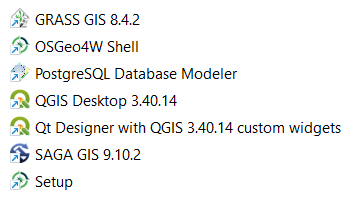
\includegraphics{./images/aplicaciones_desktop_osgeo4w.png}

}

\caption{\label{fig-aplicaciones_desktop_osgeo4w}Aplicaciones Desktop
OSGeo4W.}

\end{figure}%

\subsection{Instrucciones de
Instalación}\label{instrucciones-de-instalaciuxf3n}

\begin{enumerate}
\def\labelenumi{\arabic{enumi}.}
\tightlist
\item
  Descargue el \href{https://qgis.org/download/}{\textbf{Network
  Installer}} de QGIS.
\item
  Ejecute y seleccione \textbf{Advanced Install}.
\item
  Mantenga las rutas por defecto (\texttt{C:\textbackslash{}OSGeo4W}).
\item
  En el paso de \textbf{Select Packages}, busque los elementos de la
  tabla y marque únicamente la casilla \textbf{Bin} (Binarios).
\end{enumerate}

\subsection{Lista de paquetes a
seleccionar}\label{lista-de-paquetes-a-seleccionar}

\begin{longtable}[]{@{}
  >{\raggedright\arraybackslash}p{(\columnwidth - 6\tabcolsep) * \real{0.2500}}
  >{\raggedright\arraybackslash}p{(\columnwidth - 6\tabcolsep) * \real{0.2500}}
  >{\raggedright\arraybackslash}p{(\columnwidth - 6\tabcolsep) * \real{0.2500}}
  >{\raggedright\arraybackslash}p{(\columnwidth - 6\tabcolsep) * \real{0.2500}}@{}}
\caption{Listado de herramientas y librerías OSGeo4W para el
curso}\label{tbl-stack-software-osgeo4w}\tabularnewline
\toprule\noalign{}
\begin{minipage}[b]{\linewidth}\raggedright
Grupo
\end{minipage} & \begin{minipage}[b]{\linewidth}\raggedright
Paquete
\end{minipage} & \begin{minipage}[b]{\linewidth}\raggedright
Módulo
\end{minipage} & \begin{minipage}[b]{\linewidth}\raggedright
Propósito / Uso en Clase
\end{minipage} \\
\midrule\noalign{}
\endfirsthead
\toprule\noalign{}
\begin{minipage}[b]{\linewidth}\raggedright
Grupo
\end{minipage} & \begin{minipage}[b]{\linewidth}\raggedright
Paquete
\end{minipage} & \begin{minipage}[b]{\linewidth}\raggedright
Módulo
\end{minipage} & \begin{minipage}[b]{\linewidth}\raggedright
Propósito / Uso en Clase
\end{minipage} \\
\midrule\noalign{}
\endhead
\bottomrule\noalign{}
\endlastfoot
\textbf{Entorno Core} & \texttt{qgis-ltr} / \texttt{qgis-ltr-full} &
Todo & Software base y metapaquete de dependencias. \\
\textbf{Bases de Datos} & \texttt{pgmodeler} & 5 & Diseño visual de
modelos para PostGIS. \\
\textbf{Bases de Datos} & \texttt{libspatialite} & 5 & Motor de base de
datos espacial liviano para verificación en shell. \\
\textbf{Bases de Datos} & \texttt{python3-psycopg2} & 5 & Adaptador de
Python para PostgreSQL/PostGIS. \\
\textbf{Geoprocesamiento} & \texttt{grass} & 6 & Motor para análisis
topológico e hidrología. \\
\textbf{Geoprocesamiento} & \texttt{saga} & 7 & Algoritmos de terreno y
geomorfometría. \\
\textbf{Geoprocesamiento} & \texttt{gdal} & 6 & Lectura/escritura de
formatos raster y vector. \\
\textbf{Ciencia de Datos} & \texttt{python3-numpy} & 2 & Manejo de
estructuras Arrays y Matrices. \\
\textbf{Ciencia de Datos} & \texttt{python3-pandas} & 3 & Análisis
exploratorio de datos (EDA). \\
\textbf{Ciencia de Datos} & \texttt{python3-geopandas} & 3 & Extensión
espacial para GeoDataFrames. \\
\textbf{Visualización} & \texttt{python3-matplotlib} & 3 & Gráficos
básicos y mapas estáticos. \\
\textbf{Visualización} & \texttt{python3-seaborn} & 3 & Gráficos
estadísticos avanzados. \\
\textbf{Desarrollo} & \texttt{python3-pip} & 1 & Gestor para instalar
librerías adicionales. \\
\textbf{Desarrollo} & \texttt{python3-jupyterlab} & Todo & Entorno
interactivo para prototipado rápido
(\citeproc{ref-wijayaningrum2022jupyter}{Wijayaningrum et~al.,
2022}). \\
\textbf{Motores SIG} & \texttt{proj} / \texttt{geos} & 6 & Cálculos de
proyecciones y geometría. \\
\textbf{Machine Learning} & \texttt{python3-scikit-learn} & 6 & Modelado
predictivo espacial. \\
\end{longtable}

\begin{tcolorbox}[enhanced jigsaw, opacityback=0, left=2mm, colbacktitle=quarto-callout-important-color!10!white, leftrule=.75mm, breakable, titlerule=0mm, rightrule=.15mm, bottomrule=.15mm, arc=.35mm, colback=white, colframe=quarto-callout-important-color-frame, opacitybacktitle=0.6, toptitle=1mm, title=\textcolor{quarto-callout-important-color}{\faExclamation}\hspace{0.5em}{Aceptación de Dependencias Adicionales}, bottomtitle=1mm, toprule=.15mm, coltitle=black]

Al avanzar, el instalador mostrará la ventana \textbf{``Unmet
Dependencies''}. Es obligatorio aceptar todos los paquetes sugeridos
para contar con los controladores de formatos \texttt{.ecw} y
\texttt{.sid} requeridos por la cartografía oficial nacional. Para que
el comando \texttt{spatialite} funcione en la shell, asegúrese de marcar
el paquete \texttt{libspatialite} en la sección \textbf{Libs}.

\end{tcolorbox}

\subsection{Verificación de la
Instalación}\label{verificaciuxf3n-de-la-instalaciuxf3n}

Abra la \textbf{OSGeo4W Shell} y ejecute los comandos para verificar la
correcta integración de Python y los motores SIG:

\begin{Shaded}
\begin{Highlighting}[]
\ExtensionTok{python3} \AttributeTok{{-}{-}version}
\ExtensionTok{gdalinfo} \AttributeTok{{-}{-}version}
\ExtensionTok{spatialite} \AttributeTok{{-}{-}version}
\end{Highlighting}
\end{Shaded}

\subsubsection{Corrección de Errores al Lanzar
QGIS}\label{correcciuxf3n-de-errores-al-lanzar-qgis}

Si al iniciar QGIS aparece un error crítico indicando
\texttt{ModuleNotFoundError:\ No\ module\ named\ \textquotesingle{}gdal\textquotesingle{}},
se debe a una sintaxis de importación obsoleta en ciertos complementos
(\citeproc{ref-rosas2022qgis}{Rosas-Chavoya et~al., 2022}).

\textbf{Error identificado:}
\texttt{File\ ".../agknow\_utils.py",\ line\ 29,\ in\ \textless{}module\textgreater{}\ import\ gdal,\ osr}

\textbf{Solución:} Debe modificar el archivo del plugin para usar el
espacio de nombres de OSGeo:

\begin{enumerate}
\def\labelenumi{\arabic{enumi}.}
\item
  Localice el archivo en:
  \texttt{\%AppData\%\textbackslash{}QGIS\textbackslash{}QGIS3\textbackslash{}profiles\textbackslash{}default\textbackslash{}python\textbackslash{}plugins\textbackslash{}agknow\_qgis\textbackslash{}agknow\_utils.py}.
\item
  Reemplace la línea 29:

  \begin{itemize}
  \tightlist
  \item
    \textbf{Incorrecto:} \texttt{import\ gdal,\ osr}
  \item
    \textbf{Correcto:} \texttt{from\ osgeo\ import\ gdal,\ osr}
  \end{itemize}
\end{enumerate}

\begin{tcolorbox}[enhanced jigsaw, opacityback=0, left=2mm, colbacktitle=quarto-callout-note-color!10!white, leftrule=.75mm, breakable, titlerule=0mm, rightrule=.15mm, bottomrule=.15mm, arc=.35mm, colback=white, colframe=quarto-callout-note-color-frame, opacitybacktitle=0.6, toptitle=1mm, title=\textcolor{quarto-callout-note-color}{\faInfo}\hspace{0.5em}{Nota sobre R y Julia}, bottomtitle=1mm, toprule=.15mm, coltitle=black]

Para el uso intensivo de R y Julia, se recomienda la \textbf{Opción A
(Docker)} (\citeproc{ref-docker2025}{Inc., 2025}) ya que viene con las
librerías espaciales pre-configuradas, evitando errores de vinculación
de DLLs comunes en instalaciones nativas de Windows.

\end{tcolorbox}

\section{Opción B.2: QGIS + GEE usando Pixi}\label{sec-qgis-gee-pixi}

Antes de comenzar, es indispensable contar con una cuenta de
\textbf{Google Cloud} habilitada para \textbf{Google Earth Engine
(GEE)}. Puede dar de alta su cuenta en
\href{https://earthengine.google.com/}{earthengine.google.com}.

\begin{tcolorbox}[enhanced jigsaw, opacityback=0, left=2mm, colbacktitle=quarto-callout-important-color!10!white, leftrule=.75mm, breakable, titlerule=0mm, rightrule=.15mm, bottomrule=.15mm, arc=.35mm, colback=white, colframe=quarto-callout-important-color-frame, opacitybacktitle=0.6, toptitle=1mm, title=\textcolor{quarto-callout-important-color}{\faExclamation}\hspace{0.5em}{Requisito de Google Cloud}, bottomtitle=1mm, toprule=.15mm, coltitle=black]

Asegúrese de haber creado un proyecto en la consola de Google Cloud y de
tener activadas las \textbf{APIs for Earth Engine} para dicho proyecto;
de lo contrario, el proceso de autenticación fallará.

\end{tcolorbox}

\href{https://youtu.be/LoQwc3ne0FU}{Video gúia de creación y registro en
GEE}

\begin{center}\rule{0.5\linewidth}{0.5pt}\end{center}

\subsection{Instalación de Pixi}\label{instalaciuxf3n-de-pixi}

\textbf{Pixi} es un gestor de paquetes extremadamente rápido basado en
el ecosistema de Conda, pero mucho más ligero. Permite crear entornos
aislados sin romper las librerías de su sistema operativo.

\subsubsection{\texorpdfstring{\textbf{En Linux / macOS
(bash/zsh)}}{En Linux / macOS (bash/zsh)}}\label{en-linux-macos-bashzsh}

Ejecute el siguiente comando en su terminal:

\begin{Shaded}
\begin{Highlighting}[]
\ExtensionTok{curl} \AttributeTok{{-}fsSL}\NormalTok{ https://pixi.sh/install.sh }\KeywordTok{|} \FunctionTok{sh}
\end{Highlighting}
\end{Shaded}

\textbf{Nota:} Cierre y vuelva a abrir su terminal para que
\texttt{pixi} se añada a su \texttt{PATH}. Confirme la instalación con:

\begin{Shaded}
\begin{Highlighting}[]
\ExtensionTok{pixi} \AttributeTok{{-}{-}version}
\end{Highlighting}
\end{Shaded}

\subsubsection{\texorpdfstring{\textbf{En Windows
(PowerShell)}}{En Windows (PowerShell)}}\label{en-windows-powershell}

Abra \textbf{PowerShell} (no requiere permisos de Administrador) y
ejecute:

\begin{Shaded}
\begin{Highlighting}[]
\NormalTok{powershell }\OperatorTok{{-}}\NormalTok{ExecutionPolicy Bypass }\OperatorTok{{-}}\NormalTok{c }\StringTok{"irm {-}useb https://pixi.sh/install.ps1 | iex"}
\end{Highlighting}
\end{Shaded}

Reinicie PowerShell y confirme la versión:

\begin{Shaded}
\begin{Highlighting}[]
\NormalTok{pixi }\OperatorTok{{-}{-}}\NormalTok{version}
\end{Highlighting}
\end{Shaded}

\begin{center}\rule{0.5\linewidth}{0.5pt}\end{center}

\subsection{Creación del Proyecto}\label{creaciuxf3n-del-proyecto}

Navegue hasta la carpeta (\textbf{diferente a todas las utilizadas hasta
el momento}) donde desea guardar sus trabajos y cree un nuevo proyecto
llamado \texttt{geocd}:

\begin{Shaded}
\begin{Highlighting}[]
\ExtensionTok{pixi}\NormalTok{ init geocd}
\BuiltInTok{cd}\NormalTok{ geocd}
\end{Highlighting}
\end{Shaded}

\begin{center}\rule{0.5\linewidth}{0.5pt}\end{center}

\subsection{Configuración del Entorno
Geográfico}\label{configuraciuxf3n-del-entorno-geogruxe1fico}

Instalaremos un stack potente que incluye \textbf{QGIS} y las
herramientas necesarias para trabajar con \textbf{Google Earth Engine} y
datos ráster/vectoriales en Python.

Desde la carpeta \texttt{geocd}, ejecute:

\begin{Shaded}
\begin{Highlighting}[]
\ExtensionTok{pixi}\NormalTok{ add qgis geemap geopandas xee rioxarray}
\end{Highlighting}
\end{Shaded}

\begin{tcolorbox}[enhanced jigsaw, opacityback=0, left=2mm, colbacktitle=quarto-callout-note-color!10!white, leftrule=.75mm, breakable, titlerule=0mm, rightrule=.15mm, bottomrule=.15mm, arc=.35mm, colback=white, colframe=quarto-callout-note-color-frame, opacitybacktitle=0.6, toptitle=1mm, title=\textcolor{quarto-callout-note-color}{\faInfo}\hspace{0.5em}{¿Qué estamos instalando?}, bottomtitle=1mm, toprule=.15mm, coltitle=black]

\begin{itemize}
\tightlist
\item
  \textbf{QGIS}: El software SIG profesional de uso libre mas popular.
\item
  \textbf{geemap}: Librería para visualización interactiva de GEE.
\item
  \textbf{geopandas}: Gestión de datos vectoriales.
\item
  \textbf{xee \& rioxarray}: Motores para leer cubos de datos y archivos
  ráster.
\end{itemize}

\end{tcolorbox}

\begin{center}\rule{0.5\linewidth}{0.5pt}\end{center}

\subsection{Autenticación de Earth
Engine}\label{autenticaciuxf3n-de-earth-engine}

Finalmente, debe vincular su entorno local con su cuenta de Google
Cloud. Este comando abrirá una ventana en su navegador para autorizar el
acceso:

\begin{Shaded}
\begin{Highlighting}[]
\ExtensionTok{pixi}\NormalTok{ run earthengine authenticate}
\end{Highlighting}
\end{Shaded}

Siga las instrucciones en pantalla, seleccione su proyecto de Google
Cloud y copie el código de verificación si el sistema se lo solicita.
¡Ya está listo para procesar datos satelitales a escala global!

\subsection{Lanzar QGIS a través de
PIXI}\label{lanzar-qgis-a-travuxe9s-de-pixi}

Una vez realizada la Autenticación de Google Earth Engine, puede lanzar
QGIS usando el siguiente método

\begin{itemize}
\item
  Abra el PowerShell en la carpeta dónde configuró el proyecto PIXI
  (\texttt{geocd})
\item
  Ejecute el siguiente comando:
\end{itemize}

\begin{Shaded}
\begin{Highlighting}[]
\ExtensionTok{pixi}\NormalTok{ run qgis}
\end{Highlighting}
\end{Shaded}

\subsection{Trabajar GEE dentro de
QGIS}\label{trabajar-gee-dentro-de-qgis}

Una vez que el entorno está configurado y autenticado, el siguiente paso
es integrar \textbf{Google Earth Engine} directamente en la interfaz de
QGIS. Para esto, utilizaremos el complemento desarrollado por el equipo
de \textbf{OpenGeos}: El Plugin: \textbf{GEE Data Catalog}. Este
complemento permite navegar por los miles de datasets de Earth Engine
(Sentinel, Landsat, MODIS, etc.) y cargarlos en el lienzo de QGIS con un
solo clic, utilizando el motor de procesamiento en la nube.

\subsubsection{Instalación del Plugin}\label{instalaciuxf3n-del-plugin}

\begin{enumerate}
\def\labelenumi{\arabic{enumi}.}
\tightlist
\item
  Abre QGIS usando \texttt{pixi\ run\ qgis}
\item
  Ve al menú \textbf{Complementos} \(\rightarrow\) \textbf{Administrar e
  instalar complementos\ldots{}}
\item
  Ve a la pestaña \textbf{Configuración}.
\item
  Haz clic en \textbf{Añadir\ldots{}} en la sección ``Repositorios de
  complementos''.
\item
  Asigna un nombre al repositorio, por ejemplo: \texttt{OpenGeos}.
\item
  Ingresa la URL del repositorio:
  \texttt{https://qgis.gishub.org/plugins.xml}
\item
  Haz clic en \textbf{Aceptar}.
\item
  Ve a la pestaña \textbf{Todos}.
\item
  Busca \textbf{``Earth Engine Data Catalogs''}.
\item
  Selecciona \textbf{``Earth Engine Data Catalogs''} en la lista y haz
  clic en \textbf{Instalar complemento}.
\end{enumerate}

\begin{itemize}
\item
  \textbf{Repositorio oficial:}
  \href{https://github.com/opengeos/qgis-gee-data-catalogs-plugin}{opengeos/qgis-gee-data-catalogs-plugin}
\item
  Video Guía \textbf{Earth Engine Data Catalogs Plugin for QGIS}:
  \href{https://youtu.be/nZ3D6wLKJQw}{aquí}
\item
  Video Guía \textbf{Time Series Satellite Images in Seconds}:
  \href{https://youtu.be/8IW6XqnUjgg}{aquí}
\end{itemize}

\begin{tcolorbox}[enhanced jigsaw, opacityback=0, left=2mm, colbacktitle=quarto-callout-note-color!10!white, leftrule=.75mm, breakable, titlerule=0mm, rightrule=.15mm, bottomrule=.15mm, arc=.35mm, colback=white, colframe=quarto-callout-note-color-frame, opacitybacktitle=0.6, toptitle=1mm, title=\textcolor{quarto-callout-note-color}{\faInfo}\hspace{0.5em}{Forzar autenticación GEE dentro de QGIS (PIXI)}, bottomtitle=1mm, toprule=.15mm, coltitle=black]

Si las imágenes de GEE no cargan dentro de QGIS, la
\href{https://youtu.be/nZ3D6wLKJQw?t=574}{video-guía anterior} (en el
tiempo 574 del video) muestra unos comandos alternativos a ejecutar
dentro de la consola de Python. Esos comandos se muestran a
continuación.

Abra la Consola de Python dentro de QGIS (lanzado con
\texttt{pixi\ run\ qgis}) y ejecute los siguientes comandos:

\begin{Shaded}
\begin{Highlighting}[]
\ImportTok{import}\NormalTok{ ee}

\CommentTok{\# Autenticarse con GEE}
\NormalTok{ee.Authenticate()}
\CommentTok{\#Respuesta esperada: True}

\CommentTok{\# Inicializar el Proyecto GEE}
\NormalTok{ee.Initialize(project }\OperatorTok{=} \StringTok{"Tu ID de proyecto GEE"}\NormalTok{)}
\CommentTok{\#Respuesta esperada: Nada}
\end{Highlighting}
\end{Shaded}

\end{tcolorbox}

\subsubsection{Actualizar el plugin dentro de
QGIS}\label{actualizar-el-plugin-dentro-de-qgis}

En el manú \texttt{GEE\ Data\ Catalogs}, asegúrece de ejecutar
\texttt{Check\ for\ Updates}.

\section{Otras referencias
importantes}\label{otras-referencias-importantes}

\begin{itemize}
\tightlist
\item
  PyQGIS cookbook en markdown y Jupyter notebook formats
  (\citeproc{ref-wu2023pyqgis}{Wu, 2023a})
\item
  QGIS Notebook Plugin: Integrate Jupyter Notebooks into QGIS
  (\citeproc{ref-wu2023qgisnotebook}{Wu, 2023b})
\end{itemize}

\chapter{Guía de Instalación. Opción C: ArcGIS Pro y
ArcPy}\label{guia-C}

\section{Instalación GEE en ArcGIS Pro}\label{sec-arcgis-pro-gee}

La guía resumida de instalación y uso se encuentra en el
\href{https://www.esri.com/arcgis-blog/products/arcgis-pro/imagery/bring-google-earth-engines-data-right-into-arcgis-pro}{blog
oficial de Esri}.

\textbf{Procedimiento y requerimientos:}

\begin{enumerate}
\def\labelenumi{\arabic{enumi}.}
\tightlist
\item
  Contar con una licencia activa de ArcGIS Pro.
\item
  Instalar la caja de herramientas siguiendo el
  \href{https://github.com/gee-community/arcgis-earthengine-toolbox/blob/main/docs/03_installation.md}{procedimiento
  oficial}.
\item
  Descargar la caja de herramientas
  \href{https://github.com/gee-community/arcgis-earthengine-toolbox/releases/latest}{desde
  este enlace}.
\item
  Después de descomprimir el archivo, el procedimiento finaliza
  \href{https://pro.arcgis.com/en/pro-app/latest/help/projects/connect-to-a-toolbox.htm}{conectando
  la caja de herramientas} a tu proyecto en ArcGIS Pro.
\end{enumerate}

\subsection{Configuración del ambiente Python con
Conda}\label{configuraciuxf3n-del-ambiente-python-con-conda}

\begin{enumerate}
\def\labelenumi{\arabic{enumi}.}
\tightlist
\item
  Ejecutar \textbf{ArcGIS Python Command Prompt} como administrador:
  Ruta: \textbf{Start Menu} -\textgreater{} \textbf{All Apps}
  -\textgreater{} \textbf{ArcGIS folder} -\textgreater{} \textbf{Python
  Command Prompt} (Clic derecho \textgreater{} Ejecutar como
  administrador).
\end{enumerate}

\begin{figure}[H]

{\centering 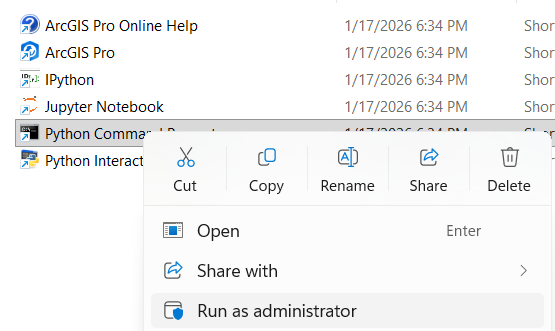
\includegraphics[width=0.6\textwidth,height=\textheight]{images/arcgispro/gee/python_commando_as_administrator.png}

}

\caption{ArcGIS Python Command Prompt como administrador}

\end{figure}%

\begin{enumerate}
\def\labelenumi{\arabic{enumi}.}
\setcounter{enumi}{1}
\tightlist
\item
  Verificar los ambientes Conda disponibles:
\end{enumerate}

\begin{Shaded}
\begin{Highlighting}[]
\ExtensionTok{conda}\NormalTok{ env list}
\end{Highlighting}
\end{Shaded}

\begin{enumerate}
\def\labelenumi{\arabic{enumi}.}
\setcounter{enumi}{2}
\tightlist
\item
  Clonar el entorno principal de ArcGIS Pro para no alterar el entorno
  por defecto:
\end{enumerate}

\begin{Shaded}
\begin{Highlighting}[]
\ExtensionTok{conda}\NormalTok{ create }\AttributeTok{{-}{-}name}\NormalTok{ gee }\AttributeTok{{-}{-}clone}\NormalTok{ arcgispro{-}py3}
\end{Highlighting}
\end{Shaded}

\emph{Mensaje de salida apenas inicia la clonación:}

\begin{Shaded}
\begin{Highlighting}[]
\ExtensionTok{Source:}\NormalTok{      C:}\DataTypeTok{\textbackslash{}P}\NormalTok{rogram Files}\DataTypeTok{\textbackslash{}A}\NormalTok{rcGIS}\DataTypeTok{\textbackslash{}P}\NormalTok{ro}\DataTypeTok{\textbackslash{}b}\NormalTok{in}\DataTypeTok{\textbackslash{}P}\NormalTok{ython}\DataTypeTok{\textbackslash{}e}\NormalTok{nvs}\DataTypeTok{\textbackslash{}a}\NormalTok{rcgispro{-}py3}
\ExtensionTok{Destination:}\NormalTok{ D:}\DataTypeTok{\textbackslash{}P}\NormalTok{rograms}\DataTypeTok{\textbackslash{}m}\NormalTok{iniforge3}\DataTypeTok{\textbackslash{}e}\NormalTok{nvs}\DataTypeTok{\textbackslash{}g}\NormalTok{ee}
\end{Highlighting}
\end{Shaded}

\begin{enumerate}
\def\labelenumi{\arabic{enumi}.}
\setcounter{enumi}{3}
\tightlist
\item
  Inicializar Conda con el shell apropiado (opcional):
\end{enumerate}

\begin{Shaded}
\begin{Highlighting}[]
\ExtensionTok{conda}\NormalTok{ init cmd.exe}
\end{Highlighting}
\end{Shaded}

\begin{enumerate}
\def\labelenumi{\arabic{enumi}.}
\setcounter{enumi}{4}
\item
  \textbf{Reiniciar} el Python Command Prompt (nuevamente como
  Administrador).
\item
  Activar el nuevo entorno \texttt{gee}:
\end{enumerate}

\begin{Shaded}
\begin{Highlighting}[]
\ExtensionTok{conda}\NormalTok{ activate gee}
\end{Highlighting}
\end{Shaded}

\begin{enumerate}
\def\labelenumi{\arabic{enumi}.}
\setcounter{enumi}{6}
\tightlist
\item
  Desactivar la verificación SSL (opcional, útil en redes corporativas
  restrictivas):
\end{enumerate}

\begin{Shaded}
\begin{Highlighting}[]
\ExtensionTok{conda}\NormalTok{ config }\AttributeTok{{-}{-}set}\NormalTok{ ssl\_verify false}
\end{Highlighting}
\end{Shaded}

\begin{enumerate}
\def\labelenumi{\arabic{enumi}.}
\setcounter{enumi}{7}
\tightlist
\item
  Instalar los paquetes necesarios de GEE desde el canal
  \texttt{conda-forge}:
\end{enumerate}

\begin{Shaded}
\begin{Highlighting}[]
\ExtensionTok{conda}\NormalTok{ install earthengine{-}api xee }\AttributeTok{{-}{-}channel}\NormalTok{ conda{-}forge}
\end{Highlighting}
\end{Shaded}

\begin{quote}
\textbf{Alternativa (Si el comando anterior falla):} \textgreater{}
Puedes usar \texttt{pip} para instalar los paquetes limpiando el entorno
e intentándolo de nuevo:

\begin{Shaded}
\begin{Highlighting}[]
\ExtensionTok{conda}\NormalTok{ deactivate}
\ExtensionTok{conda}\NormalTok{ env remove }\AttributeTok{{-}{-}name}\NormalTok{ gee}
\ExtensionTok{conda}\NormalTok{ create }\AttributeTok{{-}{-}name}\NormalTok{ gee }\AttributeTok{{-}{-}clone}\NormalTok{ arcgispro{-}py3}
\ExtensionTok{conda}\NormalTok{ activate gee}
\ExtensionTok{pip}\NormalTok{ install earthengine{-}api xee}

\CommentTok{\# Dependiendo de los warnings en consola, es posible que requieras estos paquetes:}
\ExtensionTok{pip}\NormalTok{ install }\StringTok{"pyarrow\textgreater{}=17,\textless{}21"}\NormalTok{ pywin32}
\end{Highlighting}
\end{Shaded}
\end{quote}

\begin{enumerate}
\def\labelenumi{\arabic{enumi}.}
\setcounter{enumi}{8}
\tightlist
\item
  Instalar otros paquetes requeridos desde el canal oficial de
  \texttt{esri} (dependiendo de tu versión):
\end{enumerate}

\begin{itemize}
\tightlist
\item
  Para \textbf{ArcGIS Pro 3.5 y anteriores}:
\end{itemize}

\begin{Shaded}
\begin{Highlighting}[]
\ExtensionTok{conda}\NormalTok{ install rasterio=1.3.9 }\AttributeTok{{-}{-}channel}\NormalTok{ esri}
\end{Highlighting}
\end{Shaded}

\begin{itemize}
\tightlist
\item
  Para \textbf{ArcGIS Pro 3.6 y posteriores}:
\end{itemize}

\begin{Shaded}
\begin{Highlighting}[]
\ExtensionTok{conda}\NormalTok{ install rasterio=1.4.3 }\AttributeTok{{-}{-}channel}\NormalTok{ esri}
\end{Highlighting}
\end{Shaded}

\begin{enumerate}
\def\labelenumi{\arabic{enumi}.}
\setcounter{enumi}{9}
\tightlist
\item
  Intercambiar el entorno predeterminado de ArcGIS Pro para que use
  \texttt{gee} de ahora en adelante:
\end{enumerate}

\begin{Shaded}
\begin{Highlighting}[]
\ExtensionTok{proswap}\NormalTok{ gee}
\end{Highlighting}
\end{Shaded}

\begin{enumerate}
\def\labelenumi{\arabic{enumi}.}
\setcounter{enumi}{10}
\tightlist
\item
  Cerrar el Python Command Prompt y abrir ArcGIS Pro.
\end{enumerate}

\begin{itemize}
\tightlist
\item
  El ambiente por defecto ahora será \texttt{gee}.
\item
  Verifica que los paquetes funcionen yendo a \textbf{Analysis}
  -\textgreater{} \textbf{Python} -\textgreater{} \textbf{Python Window}
  y ejecutando:
\end{itemize}

\begin{Shaded}
\begin{Highlighting}[]
\ImportTok{import}\NormalTok{ ee}
\ImportTok{import}\NormalTok{ xee}
\ImportTok{import}\NormalTok{ rasterio}
\end{Highlighting}
\end{Shaded}

\begin{center}\rule{0.5\linewidth}{0.5pt}\end{center}

\subsection{Descargar la caja de herramientas
(Toolbox)}\label{descargar-la-caja-de-herramientas-toolbox}

Puedes clonar el repositorio mediante Git:

\begin{Shaded}
\begin{Highlighting}[]
\FunctionTok{git}\NormalTok{ clone https://github.com/gee{-}community/arcgis{-}earthengine{-}toolbox.git}
\end{Highlighting}
\end{Shaded}

Alternativamente, descarga el archivo \texttt{.zip} directamente desde
\href{https://github.com/gee-community/arcgis-earthengine-toolbox}{GitHub}
y descomprímelo.

\begin{itemize}
\item
  \textbf{Opción A:} Guardar la carpeta descargada directamente en el
  directorio de tu proyecto actual:

  \texttt{C:\textbackslash{}Users\textbackslash{}\textless{}username\textgreater{}\textbackslash{}Documents\textbackslash{}ArcGIS\textbackslash{}Projects\textbackslash{}\textless{}project\_name\textgreater{}\textbackslash{}ArcGIS\ Earth\ Engine\ Toolbox}
\item
  \textbf{Opción B:} Guardar la caja de herramientas en un directorio
  global para usarla en múltiples proyectos. Por ejemplo:

  \texttt{D:\textbackslash{}Programs\textbackslash{}ArcGIS\textbackslash{}Pro\textbackslash{}arcgis-earthengine-toolbox}
\end{itemize}

\subsection{Agregar la caja de herramientas GEE a ArcGIS
Pro}\label{agregar-la-caja-de-herramientas-gee-a-arcgis-pro}

\begin{enumerate}
\def\labelenumi{\arabic{enumi}.}
\tightlist
\item
  Abre ArcGIS Pro.
\item
  En el panel \textbf{Catalog} (Catálogo), haz clic derecho en
  \textbf{Toolboxes} (Cajas de herramientas) y selecciona \textbf{Add
  Toolbox} (Agregar caja de herramientas).
\item
  Navega a la ruta donde descomprimiste los archivos (ej:
  \texttt{D:\textbackslash{}Programs\textbackslash{}ArcGIS\textbackslash{}Pro\textbackslash{}arcgis-earthengine-toolbox})
  y selecciona el archivo de la herramienta.
\end{enumerate}

\begin{figure}[H]

{\centering 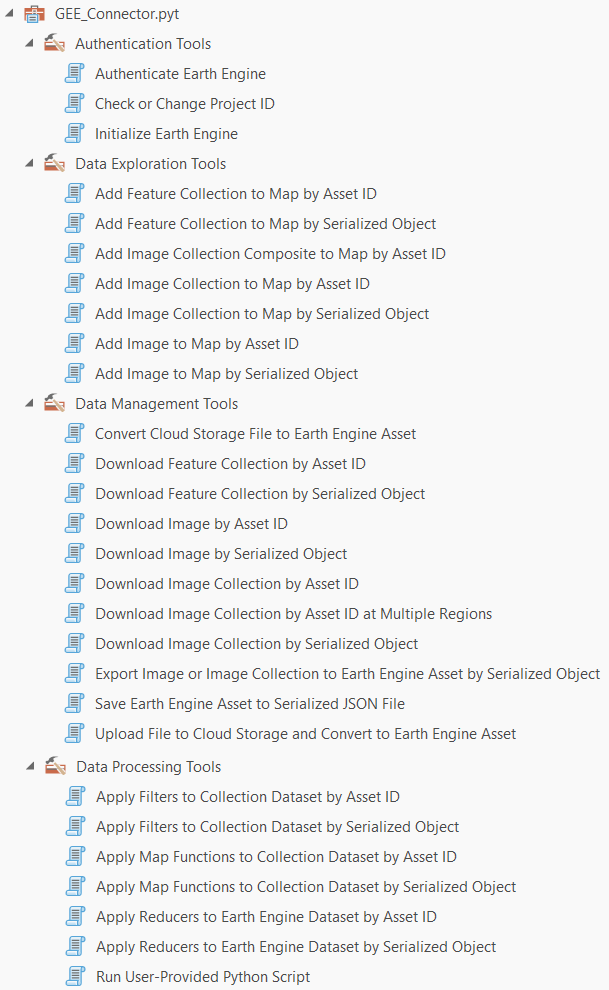
\includegraphics[width=0.7\textwidth,height=\textheight]{images/arcgispro/gee/gee_arcgispro_tool.png}

}

\caption{Caja de Herramientas GEE integrada en ArcGIS Pro}

\end{figure}%

\emph{Consulta el
\href{https://pro.arcgis.com/en/pro-app/latest/help/projects/connect-to-a-toolbox.htm}{procedimiento
oficial de Esri} si tienes dudas sobre cómo conectar una caja de
herramientas.}

\subsection{Actualizar la caja de herramientas GEE
(Opcional)}\label{actualizar-la-caja-de-herramientas-gee-opcional}

Si en el futuro requieres la versión más reciente del Toolbox, sigue el
procedimiento descrito en la
\href{https://github.com/gee-community/arcgis-earthengine-toolbox/blob/main/docs/08_upgrades.md}{documentación
oficial de actualizaciones}.

\begin{center}\rule{0.5\linewidth}{0.5pt}\end{center}

\subsection{Instalar Google Cloud SDK}\label{instalar-google-cloud-sdk}

Dado que GEE requiere validación en la nube de Google, necesitamos su
herramienta de línea de comandos. Encuentra aquí la
\href{https://docs.cloud.google.com/sdk/docs/install-sdk}{guía oficial
de instalación de Google Cloud CLI}.

\begin{enumerate}
\def\labelenumi{\arabic{enumi}.}
\tightlist
\item
  Selecciona o crea tu proyecto de Google Cloud en este
  \href{https://console.cloud.google.com/projectselector2/home/dashboard}{enlace}.
\item
  Verifica que la facturación (\textbf{Billing}) esté habilitada para tu
  proyecto
  \href{https://docs.cloud.google.com/billing/docs/how-to/verify-billing-enabled\#confirm_billing_is_enabled_on_a_project}{aquí}.
  \emph{(Nota: GEE es gratuito, pero requiere tener facturación
  configurada como protocolo de Cloud).}
\item
  Descarga el
  \href{https://dl.google.com/dl/cloudsdk/channels/rapid/GoogleCloudSDKInstaller.exe}{instalador
  de Google Cloud CLI para Windows}.
\item
  Ejecuta el instalador y sigue las instrucciones en pantalla.
\end{enumerate}

\textbf{⚠️ Importante:} Al finalizar, \textbf{desmarca} la opción de
abrir la consola (\emph{Start Google Cloud SDK Shell}).

\begin{enumerate}
\def\labelenumi{\arabic{enumi}.}
\setcounter{enumi}{4}
\tightlist
\item
  Abre una terminal de \textbf{PowerShell} y ejecuta:
\end{enumerate}

\begin{Shaded}
\begin{Highlighting}[]
\ExtensionTok{gcloud}\NormalTok{ init}
\end{Highlighting}
\end{Shaded}

\begin{itemize}
\tightlist
\item
  Se abrirá una pestaña en tu navegador web. Ingresa con tu cuenta de
  Google.
\item
  Después de autorizar, recibirás un mensaje similar a \textbf{``You are
  now authenticated with the gcloud CLI''}.
\end{itemize}

De regreso a tu consola de PowerShell:

\begin{itemize}
\tightlist
\item
  Te pedirá que indiques el número del proyecto que deseas utilizar (ej:
  \texttt{1}). Recuerda seleccionar el proyecto que tiene la facturación
  habilitada.
\item
  Dirígete a \href{https://console.developers.google.com/apis}{este
  enlace de la Consola de APIs} y asegúrate de tener tu proyecto
  seleccionado.
\item
  Ve a la pestaña \textbf{Enable API and Services}.
\item
  Busca \textbf{Compute Engine API}, selecciónala y presiona
  \textbf{Enable}. Esto permitirá a Google Cloud seleccionar una zona y
  región de cómputo automáticamente, optimizando el uso de recursos.
  (Debe aparecer activa en tu lista de APIs).
\end{itemize}

\begin{center}\rule{0.5\linewidth}{0.5pt}\end{center}

\subsection{Credenciales para GEE}\label{credenciales-para-gee}

Una vez que Google Cloud SDK está instalado, GEE utilizará sus
credenciales por defecto para autenticarte dentro de ArcGIS Pro.

\begin{enumerate}
\def\labelenumi{\arabic{enumi}.}
\tightlist
\item
  Encuentra tu \textbf{Google Cloud Project ID}:
\end{enumerate}

\begin{itemize}
\tightlist
\item
  Recuerda que el \texttt{Project\ ID} suele ser diferente al
  \texttt{Project\ Name} (típicamente tiene un formato como
  \texttt{my-project-123456}).
\item
  En la esquina superior derecha de la
  \href{https://console.cloud.google.com/}{Consola de Google Cloud}, haz
  clic en los tres puntos y selecciona \textbf{Project settings}. Allí
  podrás copiar tu \texttt{Project\ ID}.
\end{itemize}

\begin{enumerate}
\def\labelenumi{\arabic{enumi}.}
\setcounter{enumi}{1}
\item
  Abre la consola \textbf{Google Cloud SDK Shell} (búscala en el menú
  inicio de Windows).
\item
  Ejecuta el siguiente comando (esto se hace \textbf{solo la primera
  vez}):
\end{enumerate}

\begin{Shaded}
\begin{Highlighting}[]
\ExtensionTok{gcloud}\NormalTok{ auth application{-}default login}
\end{Highlighting}
\end{Shaded}

\begin{itemize}
\tightlist
\item
  Sigue el proceso en el navegador web para otorgar permisos. Al
  terminar verás el mensaje: \textbf{``You are now authenticated with
  the gcloud CLI!''}.
\item
  Esto creará un archivo de seguridad llamado
  \texttt{application\_default\_credentials.json} en tu computador.
\end{itemize}

\begin{enumerate}
\def\labelenumi{\arabic{enumi}.}
\setcounter{enumi}{3}
\tightlist
\item
  Asocia tu cuota de proyecto a esas credenciales. Ejecuta este comando
  reemplazando \texttt{TU\_PROJECT\_ID} con el ID exacto de tu proyecto:
\end{enumerate}

\begin{Shaded}
\begin{Highlighting}[]
\ExtensionTok{gcloud}\NormalTok{ auth application{-}default set{-}quota{-}project TU\_PROJECT\_ID}
\end{Highlighting}
\end{Shaded}

Si todo es correcto, recibirás una confirmación similar a:

\textbf{\texttt{Credentials\ saved\ to\ file:\ {[}C:\textbackslash{}Users\textbackslash{}tu\_usuario\textbackslash{}AppData\textbackslash{}Roaming\textbackslash{}gcloud\textbackslash{}application\_default\_credentials.json{]}}}

\begin{center}\rule{0.5\linewidth}{0.5pt}\end{center}

\section{Inicializar GEE en ArcGIS
Pro}\label{inicializar-gee-en-arcgis-pro}

Una vez configurado el entorno y descargada la caja de herramientas,
procede a inicializar Earth Engine dentro de la interfaz de ArcGIS Pro.
Para ver el paso a paso, consulta la sección
Sección~\ref{sec-arcgis-pro-initialize-gee}.

\begin{center}\rule{0.5\linewidth}{0.5pt}\end{center}

\section{URLs y enlaces de referencia
importantes}\label{urls-y-enlaces-de-referencia-importantes}

\begin{itemize}
\tightlist
\item
  Documentación oficial y
  \href{https://docs.cloud.google.com/sdk/auth_success}{tutoriales de
  Google Cloud SDK}.
\item
  Procedimiento completo de
  \href{https://github.com/gee-community/arcgis-earthengine-toolbox/blob/main/docs/03_installation.md}{instalación
  del GEE Toolbox}.
\item
  Artículo de Esri:
  \href{https://www.esri.com/arcgis-blog/products/arcgis-pro/imagery/bring-google-earth-engines-data-right-into-arcgis-pro}{Cómo
  iniciar a trabajar con GEE en ArcGIS Pro}.
\end{itemize}

\begin{center}\rule{0.5\linewidth}{0.5pt}\end{center}

\section{Fuentes de datos alternativas en ArcGIS
Pro}\label{fuentes-de-datos-alternativas-en-arcgis-pro}

Aunque Earth Engine es muy potente, existen otras fuentes masivas de
datos espaciales y catálogos en la nube que puedes aprovechar
directamente en ArcGIS Pro:

\begin{itemize}
\item
  🌐 \textbf{ArcGIS Living Atlas of the World}

  \begin{itemize}
  \tightlist
  \item
    Totalmente integrado con ArcGIS Online y ArcGIS Pro (mediante la
    pestaña \texttt{Portal} en el Catálogo).
  \item
    Guía:
    \href{https://www.esri.com/arcgis-blog/products/arcgis-living-atlas/imagery/law-imagery-layers-for-analysis}{ArcGIS
    Living Atlas ready-to-use imagery layers for analysis}
  \item
    Guía:
    \href{https://www.esri.com/arcgis-blog/products/arcgis-online/imagery/large-scale-analysis-in-arcgis-online}{Explore
    Ready-to-Use Imagery for Analysis}
  \end{itemize}
\item
  📂 \textbf{STAC Catalogs (SpatioTemporal Asset Catalogs)}

  \begin{itemize}
  \tightlist
  \item
    Permite conectar inmensas bases de datos abiertas, como el
    \href{https://planetarycomputer.microsoft.com/}{Microsoft Planetary
    Computer}.
  \item
    Conecta la información estableciendo una
    \href{https://pro.arcgis.com/en/pro-app/latest/help/data/imagery/create-a-stac-connection.htm}{conexión
    STAC en ArcGIS} y aprovechando archivos
    \href{https://github.com/Esri/arcgis-for-mpc/activity}{.asc}.
  \end{itemize}
\item
  ☁️ \textbf{Cloud sources (Almacenamiento en la nube)}

  \begin{itemize}
  \tightlist
  \item
    Conecta entornos de almacenamiento masivo directamente al Catálogo
    de ArcGIS Pro vía URLs o APIs, como por ejemplo buckets de
    \href{https://enterprise.arcgis.com/en/server/10.8/cloud/amazon/connect-to-arcgis-server-on-aws-from-arcmap.htm}{AWS
    (Amazon Web Services)}.
  \end{itemize}
\item
  🌍 \textbf{Google Earth Engine Data Catalog}

  \begin{itemize}
  \tightlist
  \item
    Operado mediante la caja de herramientas integrada. Ver
    Sección~\ref{sec-arcgis-pro-gee} y
    Sección~\ref{sec-arcgis-pro-gee-start}.
  \end{itemize}
\end{itemize}

\part{Proyecto Final}

\chapter{Guía y Estructura del Proyecto
Final}\label{guuxeda-y-estructura-del-proyecto-final}

Asignatura: Geomática General

\hfill\break

\section{Introducción al Proyecto
Final}\label{introducciuxf3n-al-proyecto-final}

El proyecto final es la oportunidad perfecta para poner en práctica
todos los conceptos de Sistemas de Información Geográfica, Sensores
Remotos, Modelos Digitales de Elevación y Cartografía Digital vistos
durante el semestre.

\textbf{Modalidad:} Trabajo en parejas (2 estudiantes).

\textbf{Objetivo principal:} Representar y analizar un fenómeno natural,
social o económico utilizando herramientas y datos espaciales.

\begin{center}\rule{0.5\linewidth}{0.5pt}\end{center}

\section{Estructura del Documento
Final}\label{estructura-del-documento-final}

Su proyecto debe documentarse siguiendo el enfoque de \emph{Open
Science} promovido en el curso. Deben entregar un documento (HTML o PDF
generado con Quarto) y alojar sus códigos/scripts en GitHub. El
documento debe contener las siguientes secciones:

\begin{enumerate}
\def\labelenumi{\arabic{enumi}.}
\tightlist
\item
  \textbf{Título del Proyecto:} Claro, conciso y descriptivo.
\item
  \textbf{Introducción y Justificación:} ¿Cuál es el problema a
  resolver? ¿Por qué es importante el contexto espacial para este
  problema?
\item
  \textbf{Objetivos:} Un objetivo general y dos o tres específicos.
\item
  \textbf{Área de Estudio:} Delimitación geográfica clara del lugar
  donde se realizará el análisis (incluir un mapa base).
\item
  \textbf{Fuentes de Datos:} Descripción de los datos espaciales a
  utilizar (ej. imágenes de Google Earth Engine, datos vectoriales de
  geoportales, MDE, etc.).
\item
  \textbf{Metodología:} Explicación paso a paso de las técnicas
  aplicadas, correcciones realizadas, cálculo de índices o modelos
  implementados.
\item
  \textbf{Resultados y Discusión:} Presentación de la cartografía
  temática generada y el análisis de lo que estos mapas nos dicen sobre
  el fenómeno estudiado.
\item
  \textbf{Conclusiones:} ¿Se cumplieron los objetivos? ¿Qué limitaciones
  encontraron?
\item
  \textbf{Referencias:} Bibliografía y fuentes de datos en formato APA.
\end{enumerate}

\begin{center}\rule{0.5\linewidth}{0.5pt}\end{center}

\section{Ideas y Temas para el Proyecto
Final}\label{ideas-y-temas-para-el-proyecto-final}

Si aún no tienen un tema definido, aquí les presentamos algunas ideas
basadas en los módulos del curso que pueden adaptar a su región de
interés:

\subsection{1. Análisis Agropecuario y Cobertura
Terrestre}\label{anuxe1lisis-agropecuario-y-cobertura-terrestre}

\begin{itemize}
\tightlist
\item
  \textbf{Monitoreo de salud de cultivos:} Uso de imágenes
  multiespectrales para calcular índices (ej. NDVI) y analizar el vigor
  agrícola.
\item
  \textbf{Dinámicas de cobertura terrestre:} Exploración de cambios de
  uso del suelo utilizando Machine Learning no supervisado (ej. K-Means
  en imágenes Sentinel-2).
  \href{https://colab.research.google.com/drive/1v2kXcbQUpnwmtiM5YQ_8H87P1t5rziW8?usp=sharing}{Ver
  ejemplo de código}.
\end{itemize}

\subsection{2. Riesgos Naturales y Modelos de
Elevación}\label{riesgos-naturales-y-modelos-de-elevaciuxf3n}

\begin{itemize}
\tightlist
\item
  \textbf{Zonificación de riesgo de inundaciones o deslizamientos:}
  Integración de MDE para derivar pendientes y redes de drenaje,
  combinados con datos de cobertura vegetal.
\item
  \textbf{Monitoreo y evaluación de daños:} Análisis de incendios
  forestales (Wildfires) o evaluación de daños a infraestructuras tras
  un desastre.
\end{itemize}

\subsection{3. Planeación Urbana y
Social}\label{planeaciuxf3n-urbana-y-social}

\begin{itemize}
\tightlist
\item
  \textbf{Accesibilidad a servicios y huella urbana:} Análisis de redes
  o clasificación de imágenes para observar la expansión de las ciudades
  y el acceso a servicios.
\item
  \textbf{Derechos Humanos:} Uso de imágenes satelitales para monitorear
  asentamientos informales o impactos en comunidades vulnerables.
\end{itemize}

\subsection{4. Navegación y Trabajo de
Campo}\label{navegaciuxf3n-y-trabajo-de-campo}

\begin{itemize}
\tightlist
\item
  \textbf{Mapeo colaborativo de infraestructura:} Creación de
  formularios de captura de datos y uso de sistemas GNSS para levantar
  información en campo.
\end{itemize}

\begin{center}\rule{0.5\linewidth}{0.5pt}\end{center}

\section{Recursos, Plataformas y Datos (Inspiración y Casos de
Uso)}\label{recursos-plataformas-y-datos-inspiraciuxf3n-y-casos-de-uso}

Para que no empiecen desde cero, exploren estas plataformas que ofrecen
casos de uso, datos abiertos y guías paso a paso:

\begin{itemize}
\tightlist
\item
  \textbf{NASA Lifelines Data Studios:} Paquetes enfocados en casos
  humanitarios (guías, dashboards y datos).
  \href{https://nasalifelines.org/data-studios/}{Visitar portal}

  \begin{itemize}
  \tightlist
  \item
    \href{https://nasalifelines.org/hfs-data-series/wildfire-early-warning-and-rapid-response/}{Incendios
    Forestales (Wildfires)}
  \item
    \href{https://nasalifelines.org/hfs-data-series/flood-early-warning-2/}{Inundaciones
    (Flooding)}
  \item
    \href{https://nasalifelines.org/hfs-data-series/landslide-risk-and-monitoring/}{Deslizamientos
    (Landslides)}
  \item
    \href{https://nasalifelines.org/hfs-data-series/building-damage-assessment/}{Evaluación
    de Daños (Damage Assessment)}
  \item
    \href{https://nasalifelines.org/hfs-data-series/human-rights/}{Derechos
    Humanos}
  \end{itemize}
\item
  \textbf{Sentinel Hub Education:} Guías para crear y visualizar índices
  satelitales (Contaminación del aire, Incendios, etc.) y uso de su
  plugin para QGIS.
  \href{https://www.sentinel-hub.com/explore/education/}{Explorar}
\item
  \textbf{NASA ARSET (Applied Remote Sensing Training Program):}
  Capacitaciones aplicadas en Agricultura, Resiliencia Climática, Salud,
  Calidad del Aire y Recursos Hídricos.
  \href{https://www.earthdata.nasa.gov/data/projects/arset}{Ver
  entrenamientos}
\item
  \textbf{EUMETSAT:} Entrenamientos específicos, como la
  \href{https://trainingevents.eumetsat.int/trui/events/2678}{Introducción
  a productos de incendios}.
\item
  \textbf{Cursos ESRI (MOOC):} Ej. \emph{GIS for Climate Action}.
  \href{https://www.esri.com/training/catalog/search/}{Ver catálogo}
\end{itemize}

\begin{center}\rule{0.5\linewidth}{0.5pt}\end{center}

\section{Soportes Tecnológicos y Retos de
Implementación}\label{soportes-tecnoluxf3gicos-y-retos-de-implementaciuxf3n}

Si quieren enfocar su proyecto final en la implementación técnica o el
desarrollo de una solución geomática avanzada, pueden elegir uno de los
siguientes retos:

\begin{enumerate}
\def\labelenumi{\arabic{enumi}.}
\tightlist
\item
  \textbf{Arquitectura de Datos Espaciales:} Estructurar una base de
  datos robusta (GeoPackage, PostGIS, Spatialite) o una File Geodatabase
  (definiendo Datasets, Dominios, Subtipos y Reglas topológicas).
\item
  \textbf{Automatización de Geoprocesamiento:} Solucionar un problema
  espacial estructurando un modelo visual usando ModelBuilder (ArcGIS) o
  el Modelador Gráfico (QGIS).
\item
  \textbf{Análisis en la Nube / Programación:} Procesar imágenes usando
  Google Earth Engine (GEE) o usar un Notebook (Jupyter/Python)
  integrado en QGIS/ArcGIS.
\item
  \textbf{Análisis Temporal Dinámico:} Generar un timelapse satelital
  utilizando el plugin \emph{GEE Timelapse} para QGIS
  (\href{https://github.com/opengeos/qgis-timelapse-plugin}{Ver
  repositorio}).
\end{enumerate}

\subsection{🚀 Nivel Avanzado: Machine Learning y
GeoAI}\label{nivel-avanzado-machine-learning-y-geoai}

Para aquellos interesados en la vanguardia tecnológica (Visión por
Computadora aplicada a SIG), pueden explorar las herramientas creadas
por Qiusheng Wu:

\begin{itemize}
\tightlist
\item
  \textbf{Herramientas GeoAI
  (\href{https://opengeoai.org/}{opengeoai.org}):}

  \begin{itemize}
  \tightlist
  \item
    \emph{Detección y Segmentación de Objetos:} Edificios, paneles
    solares, vehículos, barcos o cuerpos de agua.
  \item
    \emph{Clasificación de Coberturas Terrestres} (Segmentación
    Semántica).
  \item
    \emph{Uso de modelos de lenguaje (LLMs)} interactuando con SIG
    (``¿Cuántos edificios hay en esta imagen?'').
  \end{itemize}
\item
  \textbf{SamGeo (Segment Anything Model for Geospatial):} Adaptación
  del modelo SAM de Meta para imágenes satelitales. Permite segmentar
  imágenes mediante texto, crear máscaras interactivas y exportar
  vectores. Disponible también como
  \href{https://github.com/opengeos/segment-geospatial}{Plugin para
  QGIS}.
\end{itemize}

\begin{center}\rule{0.5\linewidth}{0.5pt}\end{center}

\section{Lecturas Recomendadas}\label{lecturas-recomendadas}

\begin{itemize}
\tightlist
\item
  Dovgyi, S. et al.~(2019). \emph{Fundamentals of remote sensing:
  history and practice}. Institute of Gifted Child of the NAPS of
  Ukraine.
\item
  Documentación oficial y \emph{How-to-Guides} de la plataforma que
  decidan utilizar.
\end{itemize}

\begin{center}\rule{0.5\linewidth}{0.5pt}\end{center}

\section{Recomendaciones Clave}\label{recomendaciones-clave}

\begin{itemize}
\tightlist
\item
  \textbf{Empiecen por los datos:} Antes de enamorarse de un tema,
  verifiquen que existan datos espaciales disponibles (geoportales,
  catálogos GEE, etc.) para su zona de estudio.
\item
  \textbf{Menos es más:} Es preferible un análisis sencillo pero
  riguroso y bien documentado, que intentar un modelo complejísimo que
  no logren terminar.
\item
  \textbf{Apóyense en las asesorías:} Utilicen las semanas destinadas a
  asesoría de proyecto final para validar su idea, su modelo de datos y
  sus fuentes de información con el profesor.
\end{itemize}

\part{Sensores Remotos}

\chapter{Fundamentos de sensores remotos:
Introducción}\label{fundamentos-de-sensores-remotos-introducciuxf3n}

\begin{quote}
\textbf{Fuente original:}
\href{https://natural-resources.canada.ca/science-data/science-research/geomatics/remote-sensing/tutorial-fundamentals-remote-sensing}{Natural
Resources Canada - Remote Sensing Tutorials}
\end{quote}

\section{¿Qué es la percepción
remota?}\label{quuxe9-es-la-percepciuxf3n-remota}

La percepción remota (o teledetección) es la disciplina científica
encargada de adquirir información sobre la superficie terrestre sin
necesidad de contacto físico directo. Este proceso se fundamenta en la
detección, el registro y el análisis de la energía electromagnética
reflejada o emitida por los objetos.

El flujo de trabajo estándar en la percepción remota, particularmente en
sistemas de imágenes, consta de siete elementos secuenciales:

\begin{figure}

\centering{

\includegraphics{images/sensores_remotos/canada/rsprocess.gif}

}

\caption{\label{fig-rsprocess}Proceso general de la percepción remota en
siete etapas}

\end{figure}%

\begin{enumerate}
\def\labelenumi{\arabic{enumi}.}
\tightlist
\item
  \textbf{Fuente de energía o iluminación (A):} Elemento que proporciona
  la energía electromagnética al objetivo.
\item
  \textbf{Radiación y atmósfera (B):} Interacción de la energía con los
  gases y partículas atmosféricas durante su trayectoria desde la fuente
  al objetivo, y del objetivo al sensor.
\item
  \textbf{Interacción con el objetivo (C):} Respuesta de la superficie
  terrestre a la energía incidente, dependiente de las propiedades
  físicas, químicas y biológicas del material.
\item
  \textbf{Registro de energía por el sensor (D):} Dispositivo remoto que
  capta y cuantifica la radiación electromagnética dispersada o emitida.
\item
  \textbf{Transmisión, recepción y procesamiento (E):} Envío electrónico
  de los datos capturados a estaciones terrestres para su conversión a
  formato digital o análogo.
\item
  \textbf{Interpretación y análisis (F):} Extracción de atributos
  relevantes de la imagen procesada mediante métodos visuales o
  digitales.
\item
  \textbf{Aplicación (G):} Uso de la información derivada para la toma
  de decisiones, resolución de problemas o modelamiento geoespacial.
\end{enumerate}

\section{Radiación
electromagnética}\label{radiaciuxf3n-electromagnuxe9tica}

El primer requisito operativo de la percepción remota pasiva es disponer
de una fuente de iluminación que emita energía en forma de radiación
electromagnética (típicamente, el Sol).

\begin{figure}

\centering{

\includegraphics{images/sensores_remotos/canada/rsenergy.gif}

}

\caption{\label{fig-rsenergy}Fuente de energía iluminando un objetivo en
la superficie terrestre}

\end{figure}%

Esta radiación se rige por los principios de la teoría ondulatoria,
componiéndose de un campo eléctrico (\(E\)) y un campo magnético (\(M\))
ortogonales entre sí, que se desplazan a la velocidad de la luz (\(c\)).

\begin{figure}

\centering{

\includegraphics{images/sensores_remotos/canada/electromag.gif}

}

\caption{\label{fig-electromag}Propagación ortogonal de los campos
eléctrico y magnético}

\end{figure}%

El comportamiento y categorización de esta radiación dependen de dos
propiedades físicas fundamentales: la \textbf{longitud de onda}
(\(\lambda\)) y la \textbf{frecuencia} (\(\nu\)). La longitud de onda es
la distancia entre dos crestas consecutivas de la onda (medida
habitualmente en micrómetros, \(\mu m\), o nanómetros, \(nm\)), mientras
que la frecuencia representa el número de ciclos ondulatorios que
atraviesan un punto fijo por unidad de tiempo (medida en Hertz, \(Hz\)).

\begin{figure}

\centering{

\includegraphics{images/sensores_remotos/canada/wvfreq.gif}

}

\caption{\label{fig-wvfreq}Representación gráfica de la longitud de onda
y la frecuencia}

\end{figure}%

Ambas variables mantienen una relación inversamente proporcional
descrita por la ecuación de la velocidad de la luz:

\begin{figure}

\centering{

\includegraphics{images/sensores_remotos/canada/equate1e.gif}

}

\caption{\label{fig-equate1e}Ecuación que relaciona velocidad de la luz,
longitud de onda y frecuencia}

\end{figure}%

A menor longitud de onda, mayor será la frecuencia, y viceversa.
Comprender esta relación es fundamental para discriminar espectralmente
las cubiertas terrestres.

\section{Espectro electromagnético}\label{espectro-electromagnuxe9tico}

El espectro electromagnético clasifica el continuo de energía desde las
ondas más cortas (rayos gamma) hasta las más largas (ondas de radio). En
percepción remota, solo regiones específicas poseen utilidad práctica.

\begin{figure}

\centering{

\includegraphics{images/sensores_remotos/canada/waveleng.gif}

}

\caption{\label{fig-waveleng}Regiones principales del espectro
electromagnético}

\end{figure}%

\subsection{Región ultravioleta (UV)}\label{regiuxf3n-ultravioleta-uv}

Es la porción de ondas más cortas aprovechables (inmediatamente
inferiores al violeta). Ciertos materiales de la superficie,
principalmente asociaciones litológicas y minerales, exhiben
fluorescencia bajo iluminación UV, permitiendo su detección.

\begin{figure}

\centering{

\includegraphics{images/sensores_remotos/canada/ultravio.gif}

}

\caption{\label{fig-ultravio}Región ultravioleta del espectro
electromagnético}

\end{figure}%

\subsection{Espectro visible}\label{espectro-visible}

Comprende las longitudes de onda detectables por el sistema visual
humano (aprox. 0.4 \(\mu m\) a 0.7 \(\mu m\)). Aunque constituye una
fracción minúscula del espectro electromagnético total, es la única
región asociada a la percepción del color.

\begin{figure}

\centering{

\includegraphics{images/sensores_remotos/canada/visible.gif}

}

\caption{\label{fig-visible}El estrecho rango del espectro visible}

\end{figure}%

\begin{figure}

\centering{

\includegraphics{images/sensores_remotos/canada/colours_e.gif}

}

\caption{\label{fig-colours}Distribución de colores según su longitud de
onda}

\end{figure}%

Los colores azul, verde y rojo actúan como colores primarios
espectrales. La luz solar, al refractarse a través de un prisma, revela
esta composición al curvar cada longitud de onda en un ángulo distinto.

\begin{figure}

\centering{

\includegraphics{images/sensores_remotos/canada/prism.gif}

}

\caption{\label{fig-prism}Descomposición de la luz blanca a través de un
prisma}

\end{figure}%

\subsection{Región infrarroja (IR)}\label{regiuxf3n-infrarroja-ir}

Abarca desde aprox. 0.7 \(\mu m\) hasta 100 \(\mu m\). Se divide
funcionalmente en dos categorías:

\begin{itemize}
\tightlist
\item
  \textbf{Infrarrojo reflejado (NIR y SWIR):} Rango de 0.7 \(\mu m\) a
  3.0 \(\mu m\). Se comporta físicamente de manera similar a la luz
  visible y registra energía solar reflejada.
\item
  \textbf{Infrarrojo térmico (TIR):} Rango de 3.0 \(\mu m\) a 100
  \(\mu m\). Registra la energía emitida diferencialmente por la Tierra
  en forma de calor (radiancia térmica).
\end{itemize}

\begin{figure}

\centering{

\includegraphics{images/sensores_remotos/canada/infrared_e.gif}

}

\caption{\label{fig-infrared}División de la región infrarroja: cercano,
medio y lejano/térmico}

\end{figure}%

\subsection{Región de microondas}\label{regiuxf3n-de-microondas}

Cubriendo longitudes de onda desde 1 \(mm\) hasta 1 \(m\), esta región
es de creciente interés geomático debido a su capacidad de penetración
atmosférica, siendo la base tecnológica de sistemas de radar.

\begin{figure}

\centering{

\includegraphics{images/sensores_remotos/canada/microwve.gif}

}

\caption{\label{fig-microwve}Región de microondas y ondas de radio}

\end{figure}%

\section{Interacciones con la
atmósfera}\label{interacciones-con-la-atmuxf3sfera}

La atmósfera terrestre modifica intrínsecamente la señal
electromagnética a través de procesos de dispersión y absorción.

\begin{figure}

\centering{

\includegraphics{images/sensores_remotos/canada/rsatmosph.gif}

}

\caption{\label{fig-rsatmosph}Atenuación de la radiación por la
atmósfera terrestre}

\end{figure}%

\subsection{Dispersión (Scattering)}\label{dispersiuxf3n-scattering}

Es la desviación de la trayectoria original de la radiación provocada
por gases y partículas. Depende directamente de la longitud de onda y la
abundancia del particulado.

\begin{figure}

\centering{

\includegraphics{images/sensores_remotos/canada/atmsct.gif}

}

\caption{\label{fig-atmsct}Mecanismos principales de dispersión
atmosférica}

\end{figure}%

\begin{itemize}
\tightlist
\item
  \textbf{Dispersión de Rayleigh:} Ocurre cuando el diámetro de las
  partículas es menor que la longitud de onda. Es el mecanismo dominante
  en las capas altas de la atmósfera, afectando severamente a las ondas
  cortas (ej. luz azul). Explica por qué, al amanecer y atardecer, la
  radiación debe recorrer una mayor distancia atmosférica, filtrando
  casi toda la onda corta y permitiendo solo la llegada de luz rojiza a
  la superficie.
\end{itemize}

\begin{figure}

\centering{

\includegraphics{images/sensores_remotos/canada/sunset_e.gif}

}

\caption{\label{fig-sunset}Efecto de la dispersión de Rayleigh en la
trayectoria solar}

\end{figure}%

\begin{itemize}
\tightlist
\item
  \textbf{Dispersión de Mie:} Producida por aerosoles (polvo, humo,
  vapor) con tamaños comparables a la longitud de onda incidente. Afecta
  típicamente longitudes de onda mayores en la baja atmósfera.
\item
  \textbf{Dispersión no selectiva:} Originada por macropartículas (como
  gotas de agua) mucho más grandes que la radiación incidente. Dispersa
  todas las longitudes de onda visibles uniformemente, razón por la cual
  las nubes resultan visualmente blancas.
\end{itemize}

\begin{figure}

\centering{

\includegraphics{images/sensores_remotos/canada/cloud.gif}

}

\caption{\label{fig-cloud}Efecto de dispersión no selectiva responsable
del color de las nubes}

\end{figure}%

\subsection{Absorción y ventanas
atmosféricas}\label{absorciuxf3n-y-ventanas-atmosfuxe9ricas}

Determinados gases (ozono, dióxido de carbono y vapor de agua) retienen
o absorben selectivamente la energía incidente.

\begin{figure}

\centering{

\includegraphics{images/sensores_remotos/canada/atmabsorb.gif}

}

\caption{\label{fig-atmabsorb}Bandas de absorción provocadas por gases
específicos}

\end{figure}%

Los dominios espectrales donde la atmósfera presenta alta transmitancia
(no absorbe significativamente la energía) se definen como
\textbf{ventanas atmosféricas}. Los sistemas satelitales están
calibrados de manera precisa para operar en coincidencia con estas
ventanas operativas.

\begin{figure}

\centering{

\includegraphics{images/sensores_remotos/canada/atmwind_e.gif}

}

\caption{\label{fig-atmwind}Espectro electromagnético mostrando las
ventanas atmosféricas y la transmitancia}

\end{figure}%

\section{Interacciones
radiación-objetivo}\label{interacciones-radiaciuxf3n-objetivo}

La energía que logra franquear la atmósfera interactúa con los
materiales terrestres a través de proporciones específicas de tres
mecanismos: \textbf{Absorción (A)}, \textbf{Transmisión (T)} y
\textbf{Reflexión (R)}.

\begin{figure}

\centering{

\includegraphics{images/sensores_remotos/canada/rsinterac.gif}

}

\caption{\label{fig-rsinterac}Dinámica de llegada e interacción de la
luz en la superficie}

\end{figure}%

\begin{figure}

\centering{

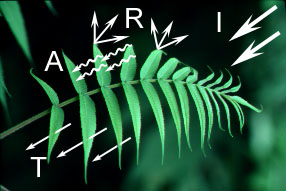
\includegraphics{images/sensores_remotos/canada/intract.jpg}

}

\caption{\label{fig-intract}Componentes de absorción, transmisión y
reflexión de la energía}

\end{figure}%

El registro teledetectado se enfoca empíricamente en la energía
reflejada. Las propiedades de esta reflexión oscilan entre dos modelos
teóricos dependiendo de la rugosidad de la superficie frente a la
longitud de onda:

\begin{itemize}
\tightlist
\item
  \textbf{Reflectancia especular:} La energía se redirige
  direccionalmente en forma de espejo (superficies lisas).
\item
  \textbf{Reflectancia difusa (lambertiana):} La energía se dispersa de
  forma isotrópica o uniforme (superficies rugosas). En el ámbito
  natural, este es el patrón predominante y deseable.
\end{itemize}

\begin{center}
\includegraphics{images/sensores_remotos/canada/speclar.gif}
\end{center}
\begin{center}
\includegraphics{images/sensores_remotos/canada/diffus.gif}
\end{center}

\subsection{Ejemplos de respuesta
material}\label{ejemplos-de-respuesta-material}

\begin{itemize}
\tightlist
\item
  \textbf{Vegetación:} La clorofila induce una fuerte absorción en el
  rojo y azul, reflejando el verde en el espectro visible.
  Simultáneamente, la estructura mesófila interna actúa como un poderoso
  reflector difuso en el infrarrojo cercano (NIR). El contraste entre la
  alta reflectancia NIR y baja reflectancia roja es el pilar de los
  índices de vegetación modernos.
\end{itemize}

\begin{figure}

\centering{

\includegraphics{images/sensores_remotos/canada/trees.gif}

}

\caption{\label{fig-trees}Interacción radiativa característica en
tejidos foliares sanos}

\end{figure}%

\begin{itemize}
\tightlist
\item
  \textbf{Agua:} Absorbe abruptamente las longitudes de onda del
  infrarrojo cercano, confiriéndole en estas bandas tonos oscuros,
  ideales para delinear litorales. En el visible, la presencia de
  sedimentos incrementa la reflectancia general, mientras que el
  plancton desplaza la respuesta pico hacia el verde.
\end{itemize}

\begin{figure}

\centering{

\includegraphics{images/sensores_remotos/canada/water.gif}

}

\caption{\label{fig-water}Absorción y reflectancia diferencial en
cuerpos de agua}

\end{figure}%

La recopilación de la magnitud de reflectancia a través de diversas
longitudes de onda conforma la \textbf{firma espectral}. El análisis
multiespectral radica en comparar firmas para discriminar taxones de
cobertura o tipologías geológicas.

\begin{figure}

\centering{

\includegraphics{images/sensores_remotos/canada/spectrl_e.gif}

}

\caption{\label{fig-spectrl}Curvas teóricas de la firma espectral para
vegetación, suelo desnudo y agua}

\end{figure}%

\section{Sensores pasivos y activos}\label{sensores-pasivos-y-activos}

Acorde al mecanismo de obtención de iluminación, la teledetección se
divide en dos tipologías principales:

\begin{itemize}
\tightlist
\item
  \textbf{Sensores pasivos:} Se limitan a registrar la radiación
  electromagnética preexistente en la naturaleza, ya sea luz solar
  reflejada (operatividad diurna) o radiación térmica emitida
  espontáneamente por los cuerpos térmicos superficiales.
\end{itemize}

\begin{figure}

\centering{

\includegraphics{images/sensores_remotos/canada/passiv.gif}

}

\caption{\label{fig-passiv}Esquema conceptual de la captura pasiva de
energía}

\end{figure}%

\begin{itemize}
\tightlist
\item
  \textbf{Sensores activos:} Incorporan su propio emisor de energía
  dirigida al objetivo, registrando el grado de retrodispersión térmica
  o lumínica resultante (backscatter). Estos instrumentos (ej. Radar SAR
  o LiDAR) superan las limitaciones climáticas y de la iluminación
  natural diurna.
\end{itemize}

\begin{figure}

\centering{

\includegraphics{images/sensores_remotos/canada/sensors.gif}

}

\caption{\label{fig-sensors}Esquema conceptual de la emisión y recepción
activa de energía}

\end{figure}%

\section{Características de las
imágenes}\label{caracteruxedsticas-de-las-imuxe1genes}

Existe una distinción metodológica crítica entre los términos
``fotografía'' e ``imagen'':

\begin{itemize}
\tightlist
\item
  \textbf{Fotografía:} Es una plasmación pictórica, obtenida sobre
  emulsiones fotoquímicas analógicas directas, frecuentemente limitadas
  al rango visible e infrarrojo próximo.
\item
  \textbf{Imagen:} Es el término integrador genérico referido a
  representaciones bidimensionales originadas electrónica o digitalmente
  desde cualquier porción del espectro electromagnético.
\end{itemize}

\begin{figure}

\centering{

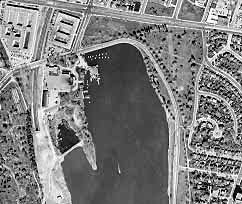
\includegraphics{images/sensores_remotos/canada/photo.jpg}

}

\caption{\label{fig-photo}Fotografía pancromática aérea tradicional
(Ottawa, Canadá)}

\end{figure}%

Las imágenes digitales se estructuran como mallas matriciales regulares
(raster). Cada celda unitaria, conocida como \textbf{píxel} (picture
element), almacena un Nivel Digital (ND) directamente correlacionado con
la radiancia de la porción terrestre muestreada.

\begin{figure}

\centering{

\includegraphics{images/sensores_remotos/canada/pixel.gif}

}

\caption{\label{fig-pixel}Estructura raster mostrando píxeles y sus
respectivos Niveles Digitales (ND)}

\end{figure}%

Los datos multiespectrales se codifican en agrupaciones espectrales
estrechas llamadas \textbf{bandas} o canales. Mientras la representación
visual de una única banda produce imágenes monocromáticas (escala de
grises), la asignación simultánea de tres bandas a los cañones de color
RGB del monitor genera \textbf{imágenes de composición en color},
elevando exponencialmente la capacidad interpretativa humana.

\begin{center}
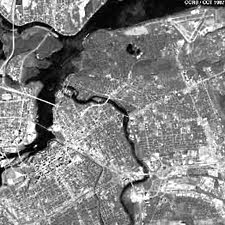
\includegraphics{images/sensores_remotos/canada/ottbw.jpg}
\end{center}
\begin{center}
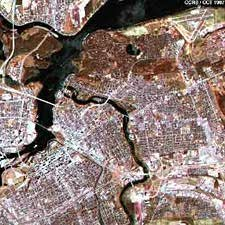
\includegraphics{images/sensores_remotos/canada/ottclr.jpg}
\end{center}

\chapter{Satélites y sensores}\label{satuxe9lites-y-sensores}

\begin{quote}
\textbf{Fuente original:}
\href{https://natural-resources.canada.ca/science-data/science-research/geomatics/remote-sensing/tutorial-fundamentals-remote-sensing}{Natural
Resources Canada - Remote Sensing Tutorials}
\end{quote}

\section{Introducción a plataformas y
sensores}\label{introducciuxf3n-a-plataformas-y-sensores}

Para que un sensor pueda captar y registrar la energía reflejada o
emitida por un objetivo, debe estar alojado en una \textbf{plataforma}
estable, aislada de la superficie observada. Estas plataformas pueden
situarse en la superficie terrestre, en la atmósfera o en el espacio.

\begin{figure}

\centering{

\includegraphics{images/sensores_remotos/canada/rsrecord.gif}

}

\caption{\label{fig-rsrecord}Registro de energía mediante sensores en
diversas plataformas. Fuente: CCRS/CCT ©}

\end{figure}%

\begin{itemize}
\tightlist
\item
  \textbf{Plataformas terrestres:} Se emplean frecuentemente para
  caracterizar detalladamente el comportamiento espectral de las
  coberturas. Esta información (``verdad terreno'') es vital para
  calibrar y validar los datos capturados por sensores aéreos y
  espaciales.
\end{itemize}

\begin{figure}

\centering{

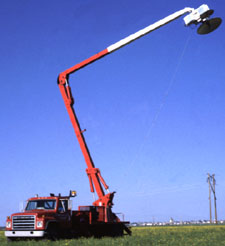
\includegraphics{images/sensores_remotos/canada/grdsens.jpg}

}

\caption{\label{fig-grdsens}Sensor montado en una plataforma terrestre.
Fuente: CCRS/CCT ©}

\end{figure}%

\begin{itemize}
\tightlist
\item
  \textbf{Plataformas aéreas:} Los aviones de ala fija son las
  plataformas atmosféricas más utilizadas. Facilitan la captura de
  imágenes de alta resolución espacial y permiten una planificación
  flexible y oportuna sobre cualquier área.
\end{itemize}

\begin{figure}

\centering{

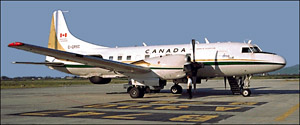
\includegraphics{images/sensores_remotos/canada/convair.jpg}

}

\caption{\label{fig-convair}Avión empleado como plataforma para
teledetección aérea. Fuente: CCRS/CCT ©}

\end{figure}%

\begin{itemize}
\tightlist
\item
  \textbf{Plataformas espaciales:} La percepción remota espacial se
  realiza desde el transbordador espacial o, mayoritariamente, desde
  satélites, los cuales permiten una cobertura sistemática, repetitiva y
  global de la superficie terrestre.
\end{itemize}

\begin{center}
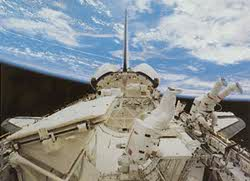
\includegraphics{images/sensores_remotos/canada/shuttle.jpg}
\end{center}
\begin{center}
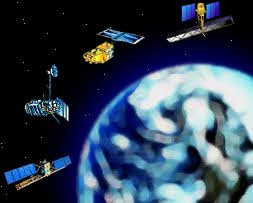
\includegraphics{images/sensores_remotos/canada/satels.jpg}
\end{center}

\section{Características orbitales y franjas de
barrido}\label{caracteruxedsticas-orbitales-y-franjas-de-barrido}

La trayectoria que sigue un satélite se denomina \textbf{órbita}. Su
diseño está estrictamente ligado a las capacidades del sensor y los
objetivos de la misión.

\begin{itemize}
\tightlist
\item
  \textbf{Órbitas geoestacionarias:} Situadas a gran altitud (aprox.
  36,000 km), su velocidad angular coincide con la rotación de la
  Tierra. El satélite permanece estacionario sobre un punto fijo, lo que
  permite la observación continua de un mismo hemisferio.
\end{itemize}

\begin{figure}

\centering{

\includegraphics{images/sensores_remotos/canada/geostation.gif}

}

\caption{\label{fig-geostation}Dinámica de una órbita geoestacionaria.
Fuente: CCRS/CCT ©}

\end{figure}%

\begin{itemize}
\tightlist
\item
  \textbf{Órbitas casi polares (Near-polar):} Siguen una trayectoria
  predominante de norte a sur. Al combinarse con la rotación terrestre,
  logran cobertura global. Comúnmente son \textbf{heliosincrónicas},
  garantizando que el satélite sobrevuele cada latitud a la misma hora
  solar local para mantener condiciones de iluminación consistentes.
\end{itemize}

\begin{figure}

\centering{

\includegraphics{images/sensores_remotos/canada/nearpolar.gif}

}

\caption{\label{fig-nearpolar}Trayectoria de una órbita casi polar y
heliosincrónica. Fuente: CCRS/CCT ©}

\end{figure}%

El trayecto de sur a norte se denomina \textbf{paso ascendente},
mientras que el trayecto de norte a sur es el \textbf{paso descendente}.
Los sensores ópticos pasivos operan casi exclusivamente durante los
pases descendentes (lado diurno).

\begin{figure}

\centering{

\includegraphics{images/sensores_remotos/canada/ascdesc.gif}

}

\caption{\label{fig-ascdesc}Representación de los pases ascendentes y
descendentes. Fuente: CCRS/CCT ©}

\end{figure}%

El área terrestre interceptada por el sensor se conoce como
\textbf{franja de barrido} (\emph{swath}). La rotación terrestre bajo la
órbita permite que cada pase barra un área diferente.

\begin{center}
\includegraphics{images/sensores_remotos/canada/swath.gif}
\end{center}
\begin{center}
\includegraphics{images/sensores_remotos/canada/orbit.gif}
\end{center}

En órbitas casi polares, el traslape (\emph{overlap}) entre franjas
adyacentes aumenta conforme la órbita se acerca a los polos.

\begin{figure}

\centering{

\includegraphics{images/sensores_remotos/canada/overlap.gif}

}

\caption{\label{fig-overlap}Aumento del traslape entre franjas
adyacentes en altas latitudes. Fuente: CCRS/CCT ©}

\end{figure}%

\section{Resolución espacial, tamaño de píxel y
escala}\label{resoluciuxf3n-espacial-tamauxf1o-de-puxedxel-y-escala}

La resolución espacial para sensores pasivos se deriva del \textbf{Campo
de Visión Instantáneo (IFOV)}, que corresponde al cono angular de
visibilidad del instrumento en un instante dado.

\begin{figure}

\centering{

\includegraphics{images/sensores_remotos/canada/fieldview.gif}

}

\caption{\label{fig-fieldview}Determinación geométrica del Campo de
Visión Instantáneo (IFOV). Fuente: CCRS/CCT ©}

\end{figure}%

Es imperativo diferenciar entre \emph{tamaño de píxel} (unidad
bidimensional de la imagen digital) y \emph{resolución espacial}
(característica física del hardware).

\begin{center}
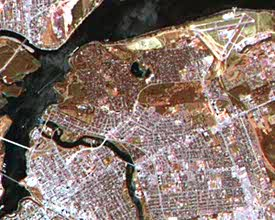
\includegraphics{images/sensores_remotos/canada/corsres.jpg}
\end{center}
\begin{center}
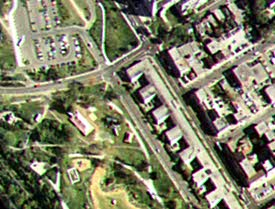
\includegraphics{images/sensores_remotos/canada/fineres.jpg}
\end{center}

La \textbf{escala} denota la relación matemática entre una dimensión en
la imagen y su magnitud real en el terreno.

\begin{center}
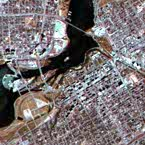
\includegraphics{images/sensores_remotos/canada/ottsat.jpg}
\end{center}
\begin{center}
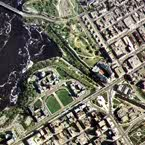
\includegraphics{images/sensores_remotos/canada/ottair.jpg}
\end{center}

\section{Resolución espectral y
radiométrica}\label{resoluciuxf3n-espectral-y-radiomuxe9trica}

La \textbf{resolución espectral} define la capacidad del sensor para
segmentar el espectro electromagnético en intervalos estrechos. Los
sensores hiperespectrales logran registrar cientos de bandas continuas
para caracterizaciones moleculares y mineralógicas precisas.

\begin{figure}

\centering{

\includegraphics{images/sensores_remotos/canada/rockcrve.gif}

}

\caption{\label{fig-rockcrve}Resolución espectral necesaria para
discriminar asociaciones litológicas. Fuente: CCRS/CCT ©}

\end{figure}%

\begin{figure}

\centering{

\includegraphics{images/sensores_remotos/canada/specrese.gif}

}

\caption{\label{fig-specrese}Esquema del particionamiento del espectro
según la resolución. Fuente: CCRS/CCT ©}

\end{figure}%

La \textbf{resolución radiométrica} determina la sensibilidad a pequeñas
variaciones de radiancia, la cual se cuantifica en bits. Una profundidad
de 8 bits permite registrar 256 niveles de gris, ofreciendo mucho mayor
contraste que imágenes de menores profundidades de bits.

\begin{center}
\includegraphics{images/sensores_remotos/canada/2bit.gif}
\end{center}
\begin{center}
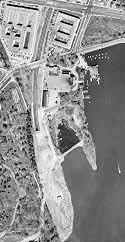
\includegraphics{images/sensores_remotos/canada/8bit.jpg}
\end{center}

\section{Resolución temporal}\label{resoluciuxf3n-temporal}

La \textbf{resolución temporal} indica la frecuencia con la que se
registra un objetivo geográfico. Plataformas con sensores orientables o
apuntables (\emph{off-nadir}) reducen drásticamente los periodos de
revisita.

\begin{figure}

\centering{

\includegraphics{images/sensores_remotos/canada/spotpoint.gif}

}

\caption{\label{fig-spotpoint}Mejora de la resolución temporal mediante
sensores de apunte lateral. Fuente: CCRS/CCT ©}

\end{figure}%

\section{Cámaras, fotografía aérea y
escaneo}\label{cuxe1maras-fotografuxeda-auxe9rea-y-escaneo}

Las cámaras aéreas de encuadre capturan simultáneamente una porción
bidimensional del terreno, ya sea en película pancromática o en falso
color infrarrojo.

\begin{figure}

\centering{

\includegraphics{images/sensores_remotos/canada/camera.gif}

}

\caption{\label{fig-camera}Geometría básica de un sistema fotográfico de
encuadre. Fuente: CCRS/CCT ©}

\end{figure}%

\begin{center}
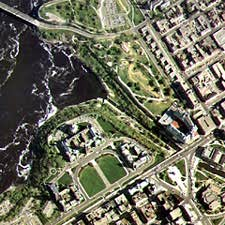
\includegraphics{images/sensores_remotos/canada/normal.jpg}
\end{center}
\begin{center}
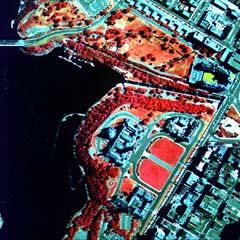
\includegraphics{images/sensores_remotos/canada/falsecolor.jpg}
\end{center}

Las adquisiciones pueden ser oblicuas o verticales, integrándose en
líneas de vuelo con alto traslape para habilitar estudios
estereoscópicos.

\begin{center}
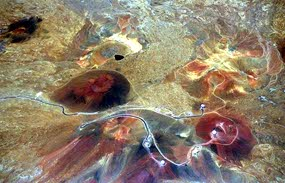
\includegraphics{images/sensores_remotos/canada/obliquept.jpg}
\end{center}
\begin{center}
\includegraphics{images/sensores_remotos/canada/flightline.gif}
\end{center}
\begin{center}
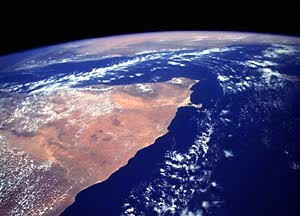
\includegraphics{images/sensores_remotos/canada/shtlpho.jpg}
\end{center}

En teledetección satelital, predominan los \textbf{sistemas de escaneo
multiespectral}: * \textbf{Barrido transversal
(Across-track/Whiskbroom):} Un espejo oscilante desvía la energía pixel
a pixel. * \textbf{Empuje lineal (Along-track/Pushbroom):} Un arreglo
lineal de detectores captura una fila completa simultáneamente,
eliminando partes móviles e incrementando el tiempo de integración.

\begin{center}
\includegraphics{images/sensores_remotos/canada/acrsstrack.gif}
\end{center}
\begin{center}
\includegraphics{images/sensores_remotos/canada/alngtrk.gif}
\end{center}

\section{Imágenes térmicas y distorsión
geométrica}\label{imuxe1genes-tuxe9rmicas-y-distorsiuxf3n-geomuxe9trica}

Los sensores térmicos detectan la emisión infrarroja natural de las
superficies. Las representaciones gráficas de temperatura aparente se
denominan \textbf{termogramas}.

\begin{center}
\includegraphics{images/sensores_remotos/canada/thermal_e.gif}
\end{center}
\begin{center}
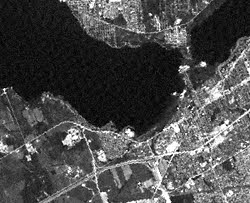
\includegraphics{images/sensores_remotos/canada/thermogram.jpg}
\end{center}

Durante la adquisición, las imágenes sufren distorsiones como el
\textbf{desplazamiento por relieve} (efecto de paralelaje respecto al
nadir) y distorsiones tangenciales propias de la cinemática del sensor.

\begin{center}
\includegraphics{images/sensores_remotos/canada/reliefdis.gif}
\end{center}
\begin{center}
\includegraphics{images/sensores_remotos/canada/geomdis.gif}
\end{center}

\section{Satélites meteorológicos}\label{satuxe9lites-meteoroluxf3gicos}

Las aplicaciones meteorológicas constituyeron uno de los primeros usos
civiles de la percepción remota. Estos satélites se caracterizan por
coberturas espaciales sumamente amplias (resolución espacial baja a
moderada) pero con muy altas frecuencias temporales.

\begin{itemize}
\tightlist
\item
  \textbf{Sistemas Geoestacionarios (ej. GOES):} Proveen vistas
  hemisféricas constantes. Son críticos para la identificación de
  dinámica atmosférica rápida y ciclones tropicales.
\end{itemize}

\begin{center}
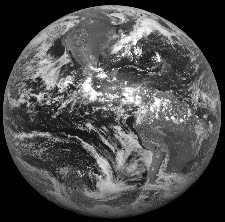
\includegraphics{images/sensores_remotos/canada/fulldsk.jpg}
\end{center}
\begin{center}
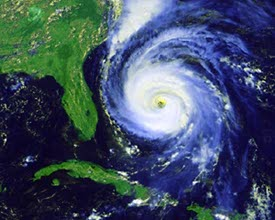
\includegraphics{images/sensores_remotos/canada/goesvw.jpg}
\end{center}

\begin{itemize}
\tightlist
\item
  \textbf{Sistemas Casi-polares (ej. NOAA AVHRR):} El sensor AVHRR opera
  sobre un \emph{swath} de casi 3000 km. Aunque concebido para el
  monitoreo del clima y la temperatura superficial del mar, ha resultado
  indispensable para derivar índices regionales de vegetación y generar
  mosaicos de usos del suelo a escala continental.
\end{itemize}

\begin{center}
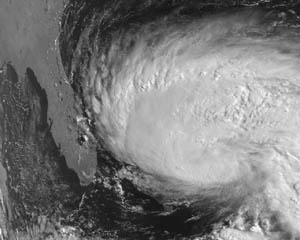
\includegraphics{images/sensores_remotos/canada/noaacld.jpg}
\end{center}
\begin{center}
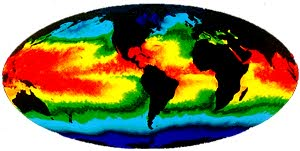
\includegraphics{images/sensores_remotos/canada/noaasst.jpg}
\end{center}
\begin{center}
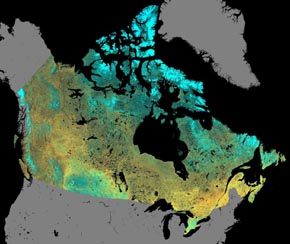
\includegraphics{images/sensores_remotos/canada/mosaic.jpg}
\end{center}

\section{Satélites de observación
terrestre}\label{satuxe9lites-de-observaciuxf3n-terrestre}

Orientados al mapeo de precisión y la gestión de recursos naturales,
estos sistemas ofrecen resoluciones espaciales finas en detrimento de la
resolución temporal (debido a barridos más estrechos).

\begin{itemize}
\tightlist
\item
  \textbf{Landsat:} Operado históricamente por NASA y NOAA, instituyó el
  monitoreo terrestre con los sensores MSS (Multispectral Scanner) y
  posteriormente el Thematic Mapper (TM). TM introdujo resolución de 30
  m, mayores anchos de banda, canales en el SWIR y cuantificación a 8
  bits.
\end{itemize}

\begin{center}
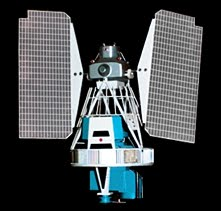
\includegraphics{images/sensores_remotos/canada/landsat2.jpg}
\end{center}
\begin{center}
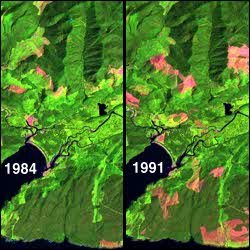
\includegraphics{images/sensores_remotos/canada/forestchg.jpg}
\end{center}

\begin{itemize}
\tightlist
\item
  \textbf{SPOT:} Desarrollado por el CNES francés. Fue pionero en
  emplear tecnología ``pushbroom'' y en permitir la orientación lateral
  de sus sensores HRV (High Resolution Visible). Esto habilitó la
  recolección estéreo para derivar Modelos Digitales de Elevación (DEM)
  y mejoró los tiempos de revisita bajo demanda.
\end{itemize}

\begin{center}
\includegraphics{images/sensores_remotos/canada/spot.gif}
\end{center}
\begin{center}
\includegraphics{images/sensores_remotos/canada/spotoff.gif}
\end{center}
\begin{center}
\includegraphics{images/sensores_remotos/canada/spotadj.gif}
\end{center}
\begin{center}
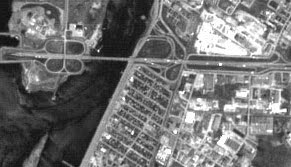
\includegraphics{images/sensores_remotos/canada/spotmap.jpg}
\end{center}

\section{Satélites de observación
marina}\label{satuxe9lites-de-observaciuxf3n-marina}

Los océanos exigen sensores calibrados para rangos de reflectancia muy
bajos y anchos de banda extremadamente finos, necesarios para penetrar
la columna de agua y evaluar variables físico-químicas.

\begin{figure}

\centering{

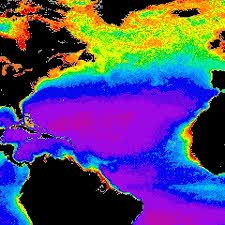
\includegraphics{images/sensores_remotos/canada/czcsclr.jpg}

}

\caption{\label{fig-czcsclr}Representación de la concentración de
fitoplancton mediante oceanografía por satélite. Fuente: CCRS/CCT ©}

\end{figure}%

Misiones como Nimbus-7 (sensor CZCS) y SeaStar (sensor SeaWiFS) fueron
diseñadas específicamente para medir la absorción de clorofila y la
dinámica del fitoplancton oceánico, parámetros fundamentales para
modelar la producción primaria y el ciclo del carbono a nivel
planetario.

\section{Otros sensores y
plataformas}\label{otros-sensores-y-plataformas}

El espectro de sensores se complementa con tecnologías de mayor
especialidad o basadas en plataformas sub-orbitales:

\begin{figure}

\centering{

\includegraphics{images/sensores_remotos/canada/othsensors.gif}

}

\caption{\label{fig-othsensors}Instrumentos no convencionales para
percepción remota. Fuente: CCRS/CCT ©}

\end{figure}%

\begin{itemize}
\tightlist
\item
  \textbf{Sistemas Láser y LiDAR:} Instrumentos activos que emiten
  pulsos de energía fotónica para determinar distancias milimétricas y
  generar perfiles tridimensionales (ej. canopeo forestal, batimetría
  somera). Los fluorosensores láser inducen y leen emisiones reactivas
  útiles en el control de vertidos marinos de hidrocarburos.
\item
  \textbf{RADAR:} Sensores activos de microondas que proveen datos
  independientemente de la cobertura nubosa o la luz diurna, vitales
  para interferometría geomorfológica o control de hielos.
\end{itemize}

\section{Recepción, transmisión y procesamiento de
datos}\label{recepciuxf3n-transmisiuxf3n-y-procesamiento-de-datos}

Los satélites de observación terrestre operan bajo una logística
rigurosa para enviar los ingentes volúmenes de datos a la superficie.

\begin{figure}

\centering{

\includegraphics{images/sensores_remotos/canada/transmit.gif}

}

\caption{\label{fig-transmit}Esquema de las arquitecturas de enlace de
datos desde la plataforma espacial al segmento terrestre. Fuente:
CCRS/CCT ©}

\end{figure}%

La transmisión de telemetría (downlink) puede ejecutarse de tres modos:
1. \textbf{Transmisión directa:} Ejecutada en tiempo real hacia una
Estación Receptora Terrestre (GRS) dentro del radio visual del satélite.
2. \textbf{Registro a bordo:} Los datos se graban temporalmente en
sistemas de estado sólido internos hasta alcanzar el alcance de una
estación de control. 3. \textbf{Satélites de retransmisión:}
Constelaciones como TDRSS interceptan la señal en órbitas altas y la
retransmiten globalmente a tierra sin interrupciones geográficas.

\begin{figure}

\centering{

\includegraphics{images/sensores_remotos/canada/gat_pass.gif}

}

\caption{\label{fig-gat_pass}Círculos de cobertura nominal de las
estaciones receptoras canadienses de Cantley y Prince Albert. Fuente:
CCRS/CCT ©}

\end{figure}%

Tras la recepción, los datos son convertidos desde su formato
radiométrico original a productos estructurados de uso final, aplicando
rectificaciones paramétricas. A nivel operativo, las estaciones suelen
generar vistas previas de baja resolución (\emph{quick-looks}) y
procesamientos en tiempo casi real orientados a respuestas de
emergencia, como navegación en mares congelados o combate de incendios.

\chapter{Sensores remotos de
microondas}\label{sensores-remotos-de-microondas}

\begin{quote}
\textbf{Fuente original:}
\href{https://natural-resources.canada.ca/science-data/science-research/geomatics/remote-sensing/tutorial-fundamentals-remote-sensing}{Natural
Resources Canada - Remote Sensing Tutorials}
\end{quote}

\section{Introducción a la percepción remota por
microondas}\label{introducciuxf3n-a-la-percepciuxf3n-remota-por-microondas}

La región de microondas del espectro electromagnético abarca longitudes
de onda desde aproximadamente 1 centímetro hasta 1 metro. Su mayor
ventaja radica en la capacidad de penetrar casi cualquier condición
atmosférica. Al ser ondas sustancialmente más largas que las partículas
atmosféricas (polvo, lluvia o nieve), no sufren dispersión severa,
operando eficazmente bajo cobertura nubosa total.

\begin{figure}

\centering{

\includegraphics{images/sensores_remotos/canada/mwrad.gif}

}

\caption{\label{fig-mwrad}Capacidad de penetración de las microondas a
través de las nubes. Fuente: CCRS/CCT ©}

\end{figure}%

\begin{itemize}
\tightlist
\item
  \textbf{Sistemas pasivos:} Detectan la escasa radiación natural de
  microondas emitida por la Tierra. Dada la baja energía, requieren
  antenas grandes y operan con resoluciones espaciales bajas. Se aplican
  en meteorología (perfiles atmosféricos), hidrología (humedad del
  suelo) y oceanografía (hielo marino).
\end{itemize}

\begin{figure}

\centering{

\includegraphics{images/sensores_remotos/canada/passmw.gif}

}

\caption{\label{fig-passmw}Concepto de teledetección pasiva en
microondas. Fuente: CCRS/CCT ©}

\end{figure}%

\begin{itemize}
\tightlist
\item
  \textbf{Sistemas activos:} Emiten su propia energía (pulsos) hacia la
  superficie y miden la retrodispersión (\emph{backscatter}). Al generar
  su iluminación, son completamente independientes de la luz solar o la
  energía térmica terrestre.
\end{itemize}

\begin{figure}

\centering{

\includegraphics{images/sensores_remotos/canada/actvmw.gif}

}

\caption{\label{fig-actvmw}Esquema de funcionamiento de un sensor activo
de microondas. Fuente: CCRS/CCT ©}

\end{figure}%

\section{Fundamentos del radar}\label{fundamentos-del-radar}

\textbf{RADAR} (RAdio Detection And Ranging) emite breves pulsos de
energía enfocados direccionalmente. Mide el tiempo de retardo entre la
emisión y la recepción del eco para determinar la distancia (rango) al
objetivo, y la intensidad del eco para caracterizarlo.

\begin{figure}

\centering{

\includegraphics{images/sensores_remotos/canada/radar.gif}

}

\caption{\label{fig-radar}Geometría básica y funcionamiento del sistema
RADAR. Fuente: CCRS/CCT ©}

\end{figure}%

El espectro se subdivide en bandas (Ka, X, C, S, L, P). La elección de
la banda define la interacción: bandas largas (L, P) penetran el dosel
forestal; bandas cortas (X, C) interactúan con el ápice foliar o
superficies expuestas.

\begin{figure}

\centering{

\includegraphics{images/sensores_remotos/canada/image2_en.gif}

}

\caption{\label{fig-image2_en}Ubicación de las bandas de microondas en
el espectro electromagnético. Fuente: CCRS/CCT ©}

\end{figure}%

\begin{center}
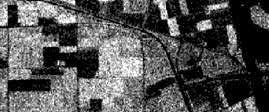
\includegraphics{images/sensores_remotos/canada/wavcomp1.jpg}
\end{center}
\begin{center}
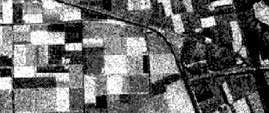
\includegraphics{images/sensores_remotos/canada/wavcomp2.jpg}
\end{center}

La \textbf{polarización} (orientación del campo eléctrico) es crítica.
Los pulsos pueden transmitirse y recibirse horizontal (H) o
verticalmente (V), generando polarizaciones equivalentes (HH, VV) o
cruzadas (HV, VH). Cada combinación ofrece respuestas únicas del
terreno.

\begin{figure}

\centering{

\includegraphics{images/sensores_remotos/canada/polari.gif}

}

\caption{\label{fig-polari}Concepto de polarización de la onda
electromagnética. Fuente: CCRS/CCT ©}

\end{figure}%

\begin{center}
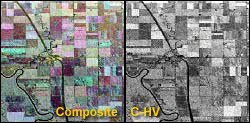
\includegraphics{images/sensores_remotos/canada/polar1.jpg}
\end{center}
\begin{center}
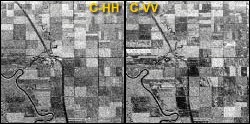
\includegraphics{images/sensores_remotos/canada/polar2.jpg}
\end{center}

\section{Geometría de visión y resolución
espacial}\label{geometruxeda-de-visiuxf3n-y-resoluciuxf3n-espacial}

El radar posee una geometría de visión lateral (\emph{side-looking}). *
\textbf{Azimut:} Dirección paralela al avance de la plataforma. *
\textbf{Rango:} Dirección transversal y ortogonal al avance.

\begin{figure}

\centering{

\includegraphics{images/sensores_remotos/canada/radgeom.gif}

}

\caption{\label{fig-radgeom}Geometría de recolección lateral mostrando
el avance (azimut) y el barrido (rango). Fuente: CCRS/CCT ©}

\end{figure}%

\begin{figure}

\centering{

\includegraphics{images/sensores_remotos/canada/range.gif}

}

\caption{\label{fig-range}Designación de las zonas de rango cercano
(near) y lejano (far). Fuente: CCRS/CCT ©}

\end{figure}%

El \textbf{ángulo de incidencia} se forma entre el haz y la normal del
terreno. El radar mide directamente la distancia en \textbf{rango
oblicuo} (\emph{slant range}), que difiere geométricamente de la
proyección horizontal real en el terreno (\emph{ground range}).

\begin{figure}

\centering{

\includegraphics{images/sensores_remotos/canada/incangl.gif}

}

\caption{\label{fig-incangl}Ángulos de incidencia y componentes de
distancia del radar. Fuente: CCRS/CCT ©}

\end{figure}%

La resolución espacial del radar es bidimensional: 1. \textbf{Resolución
en rango:} Depende de la longitud del pulso. Objetos muy cercanos en la
dirección transversal se confunden si su separación es menor a la mitad
de dicha longitud.

\begin{figure}

\centering{

\includegraphics{images/sensores_remotos/canada/rangres.gif}

}

\caption{\label{fig-rangres}Fundamento teórico de la resolución espacial
en rango. Fuente: CCRS/CCT ©}

\end{figure}%

\begin{enumerate}
\def\labelenumi{\arabic{enumi}.}
\setcounter{enumi}{1}
\tightlist
\item
  \textbf{Resolución en azimut:} Dictada por la amplitud angular del
  haz. Físicamente, requeriría antenas kilométricas en el espacio para
  mantener resolución a grandes distancias.
\end{enumerate}

\begin{figure}

\centering{

\includegraphics{images/sensores_remotos/canada/azimres.gif}

}

\caption{\label{fig-azimres}Ensanchamiento del haz afectando la
resolución en azimut. Fuente: CCRS/CCT ©}

\end{figure}%

Para resolver esto, se emplea el \textbf{Radar de Apertura Sintética
(SAR)}, que registra el historial Doppler del eco mientras la plataforma
avanza, simulando matemáticamente una antena de inmensa longitud y
logrando resoluciones finas y uniformes.

\begin{figure}

\centering{

\includegraphics{images/sensores_remotos/canada/sar.gif}

}

\caption{\label{fig-sar}Simulación de una antena larga mediante el Radar
de Apertura Sintética (SAR). Fuente: CCRS/CCT ©}

\end{figure}%

\section{Distorsiones geométricas}\label{distorsiones-geomuxe9tricas}

La reconstrucción desde el tiempo de vuelo hacia la imagen induce
severas distorsiones debido a la topografía:

\begin{itemize}
\tightlist
\item
  \textbf{Distorsión de rango oblicuo:} Comprime artificialmente la
  escala en la zona cercana de la imagen.
\end{itemize}

\begin{figure}

\centering{

\includegraphics{images/sensores_remotos/canada/slntdis.gif}

}

\caption{\label{fig-slntdis}Compresión inherente de la escala en el
rango inclinado. Fuente: CCRS/CCT ©}

\end{figure}%

\begin{center}
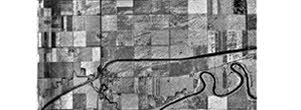
\includegraphics{images/sensores_remotos/canada/slant1.jpg}
\end{center}
\begin{center}
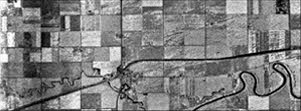
\includegraphics{images/sensores_remotos/canada/slant2.jpg}
\end{center}

\begin{itemize}
\tightlist
\item
  \textbf{Escorzo (\emph{Foreshortening}):} Las laderas enfrentadas al
  sensor devuelven el eco prematuramente, acortándose drásticamente en
  la imagen y viéndose muy brillantes.
\end{itemize}

\begin{center}
\includegraphics{images/sensores_remotos/canada/forshrt.gif}
\end{center}
\begin{center}
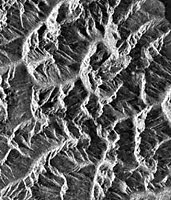
\includegraphics{images/sensores_remotos/canada/iforshrt.jpg}
\end{center}

\begin{itemize}
\tightlist
\item
  \textbf{Abatimiento (\emph{Layover}):} Caso extremo donde la cima de
  la montaña refleja la señal antes que la base, provocando que el
  relieve parezca ``caer'' hacia el sensor.
\end{itemize}

\begin{center}
\includegraphics{images/sensores_remotos/canada/layover.gif}
\end{center}
\begin{center}
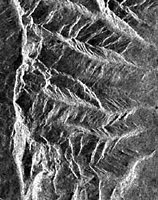
\includegraphics{images/sensores_remotos/canada/ilayovr.jpg}
\end{center}

\begin{itemize}
\tightlist
\item
  \textbf{Sombra (\emph{Shadow}):} Zonas tras el relieve (pendientes de
  espaldas) donde el haz no logra iluminar, resultando en áreas
  completamente negras (sin datos).
\end{itemize}

\begin{center}
\includegraphics{images/sensores_remotos/canada/newshadow.gif}
\end{center}
\begin{center}
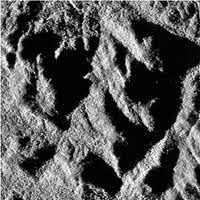
\includegraphics{images/sensores_remotos/canada/ishadow.jpg}
\end{center}

\section{Interacción con el objetivo y
apariencia}\label{interacciuxf3n-con-el-objetivo-y-apariencia}

La retrodispersión SAR depende de tres variables críticas:

\begin{enumerate}
\def\labelenumi{\arabic{enumi}.}
\tightlist
\item
  \textbf{Rugosidad superficial:} En relación a la longitud de onda.
  Superficies lisas (agua, vías) generan reflexión especular (oscuras);
  superficies rugosas (bosques) generan dispersión difusa (brillantes).
\end{enumerate}

\begin{figure}

\centering{

\includegraphics{images/sensores_remotos/canada/surfrgh.gif}

}

\caption{\label{fig-surfrgh}Concepto de rugosidad en función de la
escala de la onda. Fuente: CCRS/CCT ©}

\end{figure}%

\begin{figure}

\centering{

\includegraphics{images/sensores_remotos/canada/specdif.gif}

}

\caption{\label{fig-specdif}Comportamiento especular (A) frente a
comportamiento difuso (B). Fuente: CCRS/CCT ©}

\end{figure}%

\begin{enumerate}
\def\labelenumi{\arabic{enumi}.}
\setcounter{enumi}{1}
\tightlist
\item
  \textbf{Relación geométrica:} Evaluada mediante el ángulo de
  incidencia local. Las geometrías a 90° (estructuras urbanas) actúan
  como \textbf{reflectores de esquina}, retornando toda la energía en un
  destello brillante. La orientación del terreno respecto al haz
  (dirección de mirada) altera radicalmente el contraste.
\end{enumerate}

\begin{center}
\includegraphics{images/sensores_remotos/canada/localin.gif}
\end{center}
\begin{center}
\includegraphics{images/sensores_remotos/canada/lookdir.gif}
\end{center}

\begin{center}
\includegraphics{images/sensores_remotos/canada/corner.gif}
\end{center}
\begin{center}
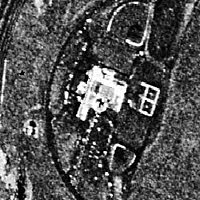
\includegraphics{images/sensores_remotos/canada/sarcity.jpg}
\end{center}

\begin{enumerate}
\def\labelenumi{\arabic{enumi}.}
\setcounter{enumi}{2}
\tightlist
\item
  \textbf{Humedad (constante dieléctrica):} La humedad incrementa la
  reflectividad radar. En condiciones extremadamente secas, la microonda
  puede penetrar la superficie, revelando estructuras subsuperficiales u
  originando interacciones de \textbf{volumen} (como el rebote múltiple
  dentro del follaje de un bosque).
\end{enumerate}

\begin{figure}

\centering{

\includegraphics{images/sensores_remotos/canada/volume.gif}

}

\caption{\label{fig-volume}Dispersión volumétrica típica en coberturas
de dosel arbóreo. Fuente: CCRS/CCT ©}

\end{figure}%

\section{Propiedades de las
imágenes}\label{propiedades-de-las-imuxe1genes}

Las imágenes SAR exhiben un granulado característico llamado
\textbf{Speckle}, derivado de la interferencia de ondas dentro de un
píxel.

\begin{center}
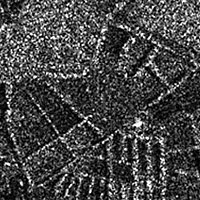
\includegraphics{images/sensores_remotos/canada/speckle.jpg}
\end{center}
\begin{center}
\includegraphics{images/sensores_remotos/canada/spkltar.gif}
\end{center}

Para reducirlo, se utiliza el procesamiento \textbf{Multi-look}
(promediando vistas durante la adquisición) o el \textbf{filtrado
espacial} post-procesamiento (promedios locales que suavizan la imagen
pero degradan levemente la resolución espacial).

\begin{center}
\includegraphics{images/sensores_remotos/canada/multilk.gif}
\end{center}
\begin{center}
\includegraphics{images/sensores_remotos/canada/avgfltr.gif}
\end{center}

\begin{center}
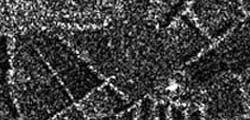
\includegraphics{images/sensores_remotos/canada/spklred1.jpg}
\end{center}
\begin{center}
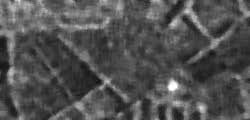
\includegraphics{images/sensores_remotos/canada/spklred2.jpg}
\end{center}

Otros ajustes vitales incluyen la corrección del \textbf{patrón de
antena} (para compensar la caída natural de energía en el rango lejano)
y la \textbf{calibración absoluta}, esencial para convertir niveles
digitales en valores de retrodispersión físicamente comparables.

\begin{figure}

\centering{

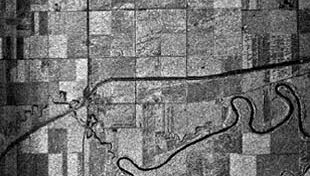
\includegraphics{images/sensores_remotos/canada/antpat.jpg}

}

\caption{\label{fig-antpat}Variación de luminosidad en el rango debido
al patrón de antena sin corregir. Fuente: CCRS/CCT ©}

\end{figure}%

\section{Aplicaciones avanzadas}\label{aplicaciones-avanzadas}

\begin{itemize}
\tightlist
\item
  \textbf{Radargrametría (Estéreo SAR):} Uso de adquisiciones con
  ángulos solapados para visión tridimensional.
\end{itemize}

\begin{figure}

\centering{

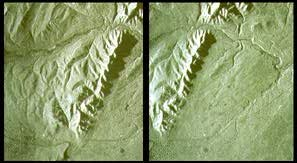
\includegraphics{images/sensores_remotos/canada/stereo2.jpg}

}

\caption{\label{fig-stereo2}Esquema de recolección estereoscópica en
microondas. Fuente: CCRS/CCT ©}

\end{figure}%

\begin{itemize}
\tightlist
\item
  \textbf{Interferometría SAR (InSAR):} Explotación de la coherencia y
  diferencia de fase para mapeo topográfico y detección de subsidencia
  milimétrica.
\end{itemize}

\begin{center}
\includegraphics{images/sensores_remotos/canada/phsedif.gif}
\end{center}
\begin{center}
\includegraphics{images/sensores_remotos/canada/isar.gif}
\end{center}

\begin{center}
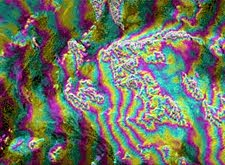
\includegraphics{images/sensores_remotos/canada/intrfer.jpg}
\end{center}
\begin{center}
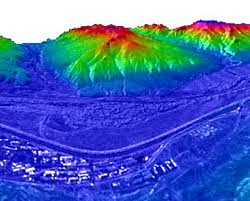
\includegraphics{images/sensores_remotos/canada/3dimg.jpg}
\end{center}

\section{Polarimetría de radar}\label{polarimetruxeda-de-radar}

Consiste en el análisis completo del estado de polarización de la onda
dispersada. Radares totalmente polarimétricos adquieren y comparan fases
y amplitudes de los 4 canales (HH, HV, VH, VV).

\begin{figure}

\centering{

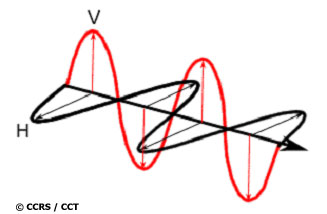
\includegraphics{images/sensores_remotos/canada/horizontal.jpg}

}

\caption{\label{fig-horizontal}Ondas ortogonales que definen los planos
de polarización. Fuente: CCRS/CCT ©}

\end{figure}%

Esta síntesis permite derivar \textbf{firmas de polarización} e imágenes
compuestas que potencian enormemente la capacidad algorítmica para
discriminar cultivos, hielos marinos y texturas forestales.

\begin{center}
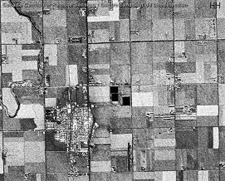
\includegraphics{images/sensores_remotos/canada/polhh.jpg}
\end{center}
\begin{center}
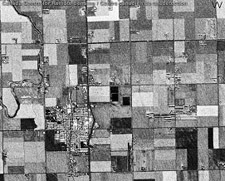
\includegraphics{images/sensores_remotos/canada/polvv.jpg}
\end{center}

\begin{center}
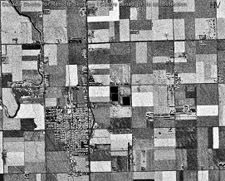
\includegraphics{images/sensores_remotos/canada/polhv.jpg}
\end{center}
\begin{center}
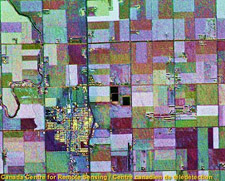
\includegraphics{images/sensores_remotos/canada/polcomp.jpg}
\end{center}

\begin{center}
\includegraphics{images/sensores_remotos/canada/copolariz.gif}
\end{center}
\begin{center}
\includegraphics{images/sensores_remotos/canada/crosspol.gif}
\end{center}

\section{Sistemas de radar aero y
espaciales}\label{sistemas-de-radar-aero-y-espaciales}

Los radares aerotransportados ofrecen agilidad, pero sus rangos de
incidencia muy variables a través de la franja acentúan los artefactos.
Los sistemas satelitales observan con ángulos consistentes desde grandes
altitudes, garantizando geometría uniforme.

\textbf{Sistemas históricos y operativos destacados:} * \textbf{Aéreos:}
Convair-580 C/X (Canadá), sistemas STAR (hielo) y AirSAR de la NASA (L,
P, C multi-polarizado).

\begin{center}
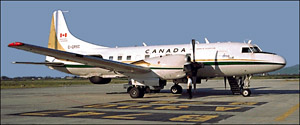
\includegraphics{images/sensores_remotos/canada/convair.jpg}
\end{center}
\begin{center}
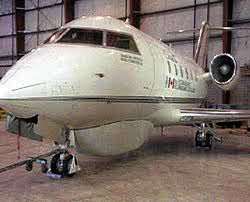
\includegraphics{images/sensores_remotos/canada/star2.jpg}
\end{center}
\begin{center}
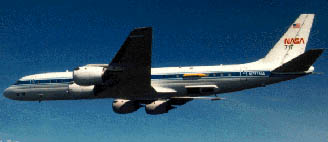
\includegraphics{images/sensores_remotos/canada/airsar.jpg}
\end{center}

\begin{itemize}
\tightlist
\item
  \textbf{Espaciales:} SEASAT (primer SAR civil), misiones europeas
  ERS-1/2, la japonesa JERS-1, y el avanzado sistema canadiense
  RADARSAT, con capacidad de direccionamiento de haz y modos escalables.
\end{itemize}

\begin{center}
\includegraphics{images/sensores_remotos/canada/seasat.gif}
\end{center}
\begin{center}
\includegraphics{images/sensores_remotos/canada/ers.gif}
\end{center}

\begin{center}
\includegraphics{images/sensores_remotos/canada/jers.gif}
\end{center}
\begin{center}
\includegraphics{images/sensores_remotos/canada/rsat.gif}
\end{center}

\begin{figure}

\centering{

\includegraphics{images/sensores_remotos/canada/rsatopt.gif}

}

\caption{\label{fig-rsatopt}Flexibilidad de barrido y modos operativos
del sistema RADARSAT. Fuente: CCRS/CCT ©}

\end{figure}%

\chapter{Análisis e interpretación de
imágenes}\label{anuxe1lisis-e-interpretaciuxf3n-de-imuxe1genes}

\begin{quote}
\textbf{Fuente original:}
\href{https://natural-resources.canada.ca/science-data/science-research/geomatics/remote-sensing/tutorial-fundamentals-remote-sensing}{Natural
Resources Canada - Remote Sensing Tutorials}
\end{quote}

\section{Introducción al análisis de
imágenes}\label{introducciuxf3n-al-anuxe1lisis-de-imuxe1genes}

La extracción de información a partir de datos teledetectados requiere
analizar las interacciones de la energía electromagnética con las
coberturas terrestres. El análisis implica la identificación y medición
de objetivos mediante dos enfoques complementarios: la
\textbf{interpretación visual} y el \textbf{procesamiento digital}.

\begin{figure}

\centering{

\includegraphics{images/sensores_remotos/canada/rs_intp.gif}

}

\caption{\label{fig-rs-intp}Análisis e interpretación en teledetección.
Fuente: CCRS/CCT ©}

\end{figure}%

\begin{itemize}
\tightlist
\item
  \textbf{Formato analógico (Interpretación Visual):} Aprovecha la
  capacidad del cerebro humano para reconocer patrones espaciales sobre
  imágenes pictóricas (impresas). Su limitación principal es la
  dificultad de evaluar simultáneamente múltiples bandas espectrales.
\end{itemize}

\begin{figure}

\centering{

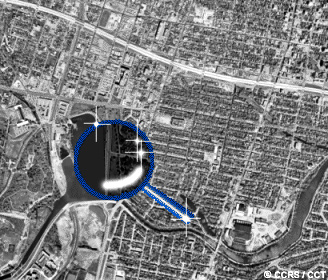
\includegraphics{images/sensores_remotos/canada/manual.jpg}

}

\caption{\label{fig-manual}Análisis analógico mediante
fotointerpretación visual. Fuente: CCRS/CCT ©}

\end{figure}%

\begin{itemize}
\tightlist
\item
  \textbf{Formato digital (Procesamiento Informático):} Los sensores
  electrónicos registran la información como matrices de Niveles
  Digitales. El entorno digital permite procesar múltiples bandas de
  forma objetiva, realzar contrastes y clasificar grandes volúmenes de
  datos con rapidez.
\end{itemize}

\begin{figure}

\centering{

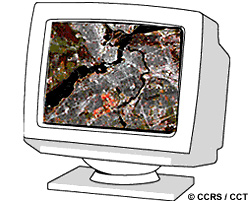
\includegraphics{images/sensores_remotos/canada/digital.jpg}

}

\caption{\label{fig-digital}Análisis digital de matrices de píxeles
mediante estaciones de trabajo. Fuente: CCRS/CCT ©}

\end{figure}%

\section{Elementos de la interpretación
visual}\label{elementos-de-la-interpretaciuxf3n-visual}

La interpretación humana se basa en el reconocimiento de siete elementos
fundamentales que definen espacialmente las coberturas:

\begin{itemize}
\tightlist
\item
  \textbf{Tono:} Es el brillo relativo o color de los objetos. Sin
  variaciones de tono, sería imposible discernir formas o texturas.
\end{itemize}

\begin{figure}

\centering{

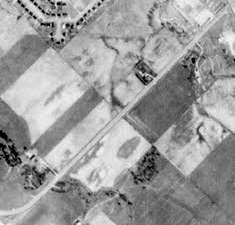
\includegraphics{images/sensores_remotos/canada/ton.jpg}

}

\caption{\label{fig-ton}Diferencias tonales que permiten delimitar
unidades espaciales. Fuente: CCRS/CCT ©}

\end{figure}%

\begin{itemize}
\tightlist
\item
  \textbf{Forma:} Contornos regulares y rectilíneos denotan intervención
  antrópica (agricultura, vías), mientras que los irregulares
  caracterizan procesos naturales.
\end{itemize}

\begin{figure}

\centering{

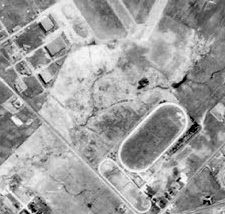
\includegraphics{images/sensores_remotos/canada/shape.jpg}

}

\caption{\label{fig-shape}Formas geométricas regulares propias de la
actividad agrícola. Fuente: CCRS/CCT ©}

\end{figure}%

\begin{itemize}
\tightlist
\item
  \textbf{Tamaño:} Evaluado según la escala de la imagen, discrimina
  objetos funcionalmente similares pero jerárquicamente distintos (ej.
  fábricas vs.~residencias).
\end{itemize}

\begin{figure}

\centering{

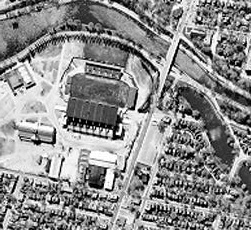
\includegraphics{images/sensores_remotos/canada/size.jpg}

}

\caption{\label{fig-size}El tamaño relativo asiste en la discriminación
de infraestructuras. Fuente: CCRS/CCT ©}

\end{figure}%

\begin{itemize}
\tightlist
\item
  \textbf{Patrón:} La repetición espacial ordenada. Huertos o zonas
  urbanas muestran patrones estructurados, a diferencia de la
  distribución aleatoria silvestre.
\end{itemize}

\begin{figure}

\centering{

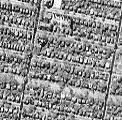
\includegraphics{images/sensores_remotos/canada/pattern.jpg}

}

\caption{\label{fig-pattern}Patrones repetitivos espaciales en
ordenación territorial. Fuente: CCRS/CCT ©}

\end{figure}%

\begin{itemize}
\tightlist
\item
  \textbf{Textura:} La frecuencia de variación tonal (``rugosidad''). Un
  bosque denso presenta textura rugosa, mientras que una pradera o el
  asfalto lucen lisos.
\end{itemize}

\begin{figure}

\centering{

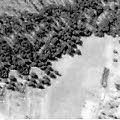
\includegraphics{images/sensores_remotos/canada/texture.jpg}

}

\caption{\label{fig-texture}Contraste de texturas entre vegetación y
superficies lisas. Fuente: CCRS/CCT ©}

\end{figure}%

\begin{itemize}
\tightlist
\item
  \textbf{Sombra:} Ayuda a perfilar el relieve tridimensional y facilita
  la identificación de estructuras verticales, aunque oculta la
  radiometría de lo que cubre.
\end{itemize}

\begin{figure}

\centering{

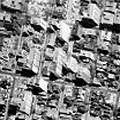
\includegraphics{images/sensores_remotos/canada/shadow.jpg}

}

\caption{\label{fig-shadow}Sombras proyectadas de perfiles topográficos
o elementos verticales. Fuente: CCRS/CCT ©}

\end{figure}%

\begin{itemize}
\tightlist
\item
  \textbf{Asociación:} Inferencia por contexto geográfico. Ej. zonas
  residenciales asociadas a escuelas, o embarcaciones asociadas a
  cuerpos de agua.
\end{itemize}

\begin{figure}

\centering{

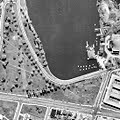
\includegraphics{images/sensores_remotos/canada/assoc.jpg}

}

\caption{\label{fig-assoc}Asociación contextual entre coberturas y usos
del suelo. Fuente: CCRS/CCT ©}

\end{figure}%

\section{Procesamiento digital de
imágenes}\label{procesamiento-digital-de-imuxe1genes}

El procesamiento implica la manipulación de los valores radiométricos en
estaciones de trabajo para facilitar la interpretación o la
clasificación automática.

\begin{figure}

\centering{

\includegraphics{images/sensores_remotos/canada/ias.gif}

}

\caption{\label{fig-ias}Arquitectura de un sistema de análisis de
imágenes. Fuente: CCRS/CCT ©}

\end{figure}%

Se estructura en cuatro categorías: 1. \textbf{Pre-procesamiento:}
Correcciones radiométricas y geométricas. 2. \textbf{Realce
(\emph{Enhancement}):} Optimización del contraste visual. 3.
\textbf{Transformaciones:} Operaciones entre múltiples bandas. 4.
\textbf{Clasificación y análisis:} Mapeo temático de la imagen.

\begin{center}
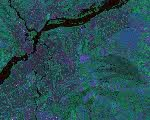
\includegraphics{images/sensores_remotos/canada/enhan1.jpg}
\end{center}
\begin{center}
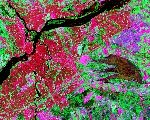
\includegraphics{images/sensores_remotos/canada/enhan2.jpg}
\end{center}

\begin{figure}

\centering{

\includegraphics{images/sensores_remotos/canada/class.gif}

}

\caption{\label{fig-class}Esquema conceptual de la clasificación de
datos. Fuente: CCRS/CCT ©}

\end{figure}%

\section{Pre-procesamiento}\label{pre-procesamiento}

Busca corregir los errores introducidos por el sensor y la geometría de
adquisición.

\textbf{Correcciones radiométricas:} * \textbf{Mosaicos:} Corrige las
variaciones de iluminación para poder unir sin costuras múltiples
imágenes contiguas.

\begin{figure}

\centering{

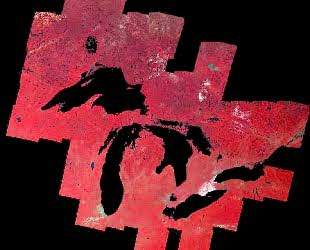
\includegraphics{images/sensores_remotos/canada/glakes.jpg}

}

\caption{\label{fig-glakes}Mosaico de múltiples imágenes corregidas
radiométricamente. Fuente: CCRS/CCT ©}

\end{figure}%

\begin{itemize}
\tightlist
\item
  \textbf{Corrección atmosférica:} Resta los valores mínimos observados
  (ej. en sombras profundas o lagos claros) para eliminar el brillo
  añadido por la dispersión atmosférica.
\end{itemize}

\begin{figure}

\centering{

\includegraphics{images/sensores_remotos/canada/atmcorr.gif}

}

\caption{\label{fig-atmcorr}Mecanismo para atenuar la dispersión
atmosférica. Fuente: CCRS/CCT ©}

\end{figure}%

\begin{itemize}
\tightlist
\item
  \textbf{Bandeado (\emph{Striping}) y líneas perdidas:} El bandeado por
  descalibración de detectores se ecualiza; las líneas faltantes por
  fallos de registro se interpolan con los valores adyacentes.
\end{itemize}

\begin{center}
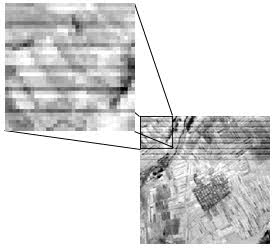
\includegraphics{images/sensores_remotos/canada/strip.jpg}
\end{center}
\begin{center}
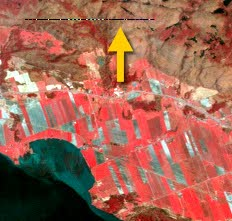
\includegraphics{images/sensores_remotos/canada/nois.jpg}
\end{center}

\textbf{Correcciones geométricas:} Rectifican distorsiones para que la
imagen concuerde con coordenadas reales. Requiere Puntos de Control
Terrestre (GCP).

\begin{figure}

\centering{

\includegraphics{images/sensores_remotos/canada/geomreg.gif}

}

\caption{\label{fig-geomreg}Proceso de emparejamiento entre coordenadas
de la imagen y un mapa base. Fuente: CCRS/CCT ©}

\end{figure}%

Para reubicar los valores en la nueva cuadrícula, se emplea el
\textbf{remuestreo}: 1. \textbf{Vecino más cercano:} Conserva valores
originales, pero produce bordes escalonados. 2. \textbf{Interpolación
bilineal:} Promedia 4 píxeles cercanos. 3. \textbf{Convolución cúbica:}
Promedia 16 píxeles, logrando la mejor estética visual.

\begin{center}
\includegraphics{images/sensores_remotos/canada/nnsamp_e.gif}
\end{center}
\begin{center}
\includegraphics{images/sensores_remotos/canada/blsamp_e.gif}
\end{center}
\begin{center}
\includegraphics{images/sensores_remotos/canada/ccsamp_e.gif}
\end{center}

\section{Realce de imágenes}\label{realce-de-imuxe1genes}

Maximiza el contraste operando sobre el \textbf{histograma} de la
imagen.

\begin{figure}

\centering{

\includegraphics{images/sensores_remotos/canada/hstogrm.gif}

}

\caption{\label{fig-hstogrm}Representación gráfica del histograma de una
imagen. Fuente: CCRS/CCT ©}

\end{figure}%

\begin{itemize}
\tightlist
\item
  \textbf{Expansión de contraste lineal:} Estira los valores mínimo y
  máximo de la imagen cruda para que ocupen todo el rango dinámico de la
  pantalla.
\end{itemize}

\begin{figure}

\centering{

\includegraphics{images/sensores_remotos/canada/linstre.gif}

}

\caption{\label{fig-linstre}Lógica de expansión lineal del histograma.
Fuente: CCRS/CCT ©}

\end{figure}%

\begin{itemize}
\tightlist
\item
  \textbf{Ecualización del histograma:} Redistribución no lineal que
  asigna más rango a los valores más frecuentes en la imagen, acentuando
  sutiles detalles locales.
\end{itemize}

\begin{figure}

\centering{

\includegraphics{images/sensores_remotos/canada/equalste.gif}

}

\caption{\label{fig-equalste}Redistribución por ecualización de
histograma. Fuente: CCRS/CCT ©}

\end{figure}%

\textbf{Filtrado espacial:} Usa una ventana móvil para alterar la
``frecuencia espacial''. Los filtros \textbf{paso bajo} suavizan la
imagen (útiles en radar). Los filtros \textbf{paso alto} acentúan bordes
y estructuras finas.

\begin{figure}

\centering{

\includegraphics{images/sensores_remotos/canada/filter.gif}

}

\caption{\label{fig-filter}Operación de matriz de convolución (filtro
espacial). Fuente: CCRS/CCT ©}

\end{figure}%

\begin{center}
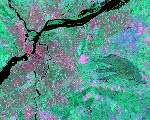
\includegraphics{images/sensores_remotos/canada/linear.jpg}
\end{center}
\begin{center}
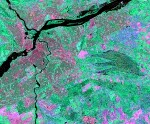
\includegraphics{images/sensores_remotos/canada/lowpass.jpg}
\end{center}

\section{Transformaciones de
imágenes}\label{transformaciones-de-imuxe1genes}

Operaciones algebraicas sobre dos o más canales espectrales. *
\textbf{Sustracción de imágenes:} Resta los píxeles de imágenes de
distintas fechas. Lo que no cambia tiende a gris medio; los cambios
bruscos (ej. deforestación) quedan muy claros u oscuros.

\begin{figure}

\centering{

\includegraphics{images/sensores_remotos/canada/subtract.gif}

}

\caption{\label{fig-subtract}Sustracción temporal revelando
deforestación. Fuente: CCRS/CCT ©}

\end{figure}%

\begin{itemize}
\tightlist
\item
  \textbf{Cálculo de cocientes (Ratioing):} Dividir una banda por otra
  reduce el efecto de las sombras por topografía abrupta. Permite
  derivar índices vitales como el \textbf{NDVI}, que evalúa el vigor
  fotosintético.
\end{itemize}

\begin{figure}

\centering{

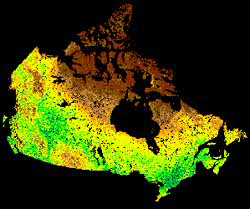
\includegraphics{images/sensores_remotos/canada/ndvi.jpg}

}

\caption{\label{fig-ndvi}Cartografía de la biomasa derivada del índice
NDVI. Fuente: CCRS/CCT ©}

\end{figure}%

\begin{itemize}
\tightlist
\item
  \textbf{Análisis de Componentes Principales (PCA):} Condensa
  estadísticamente la información redundante de múltiples bandas en solo
  2 o 3 nuevos ``componentes'' que capturan casi toda la varianza de la
  escena.
\end{itemize}

\begin{figure}

\centering{

\includegraphics{images/sensores_remotos/canada/pca.gif}

}

\caption{\label{fig-pca}Proyección ortogonal estadística en PCA. Fuente:
CCRS/CCT ©}

\end{figure}%

\section{Clasificación de imágenes y
análisis}\label{clasificaciuxf3n-de-imuxe1genes-y-anuxe1lisis}

Convierte el continuo radiométrico en un mapa de unidades temáticas
discretas.

\begin{itemize}
\tightlist
\item
  \textbf{Clasificación supervisada:} El analista entrena al algoritmo
  proporcionando ``áreas de muestra'' de coberturas conocidas. El
  sistema extrae las firmas estadísticas y clasifica el resto de la
  imagen según dichas firmas.
\end{itemize}

\begin{figure}

\centering{

\includegraphics{images/sensores_remotos/canada/super_e.gif}

}

\caption{\label{fig-super-e}Flujo analítico de la clasificación
supervisada. Fuente: CCRS/CCT ©}

\end{figure}%

\begin{itemize}
\tightlist
\item
  \textbf{Clasificación no supervisada:} Operación automática donde un
  algoritmo agrupa los píxeles en ``clústeres'' basándose exclusivamente
  en su distancia estadística. Posteriormente, el analista interpreta
  qué representa cada clúster.
\end{itemize}

\begin{figure}

\centering{

\includegraphics{images/sensores_remotos/canada/unsuper_e.gif}

}

\caption{\label{fig-unsuper-e}Proceso algorítmico de clasificación no
supervisada. Fuente: CCRS/CCT ©}

\end{figure}%

\section{Integración de datos y
SIG}\label{integraciuxf3n-de-datos-y-sig}

El análisis moderno requiere fusionar diversas fuentes
georreferenciadas.

\begin{figure}

\centering{

\includegraphics{images/sensores_remotos/canada/dataint.gif}

}

\caption{\label{fig-dataint}Fusión conceptual de múltiples fuentes de
datos. Fuente: CCRS/CCT ©}

\end{figure}%

Se puede integrar alta resolución espacial pancromática con
multiespectral gruesa (ej. SPOT), o fusionar espectro óptico con textura
de Radar SAR para potenciar la discriminación.

\begin{center}
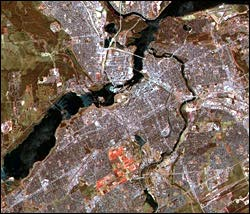
\includegraphics{images/sensores_remotos/canada/spotmrg.jpg}
\end{center}
\begin{center}
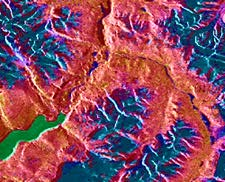
\includegraphics{images/sensores_remotos/canada/opt_sar.jpg}
\end{center}

Sumar Modelos Digitales de Elevación (DEM) permite compensar efectos
topográficos y generar vistas en perspectiva 3D.

\begin{figure}

\centering{

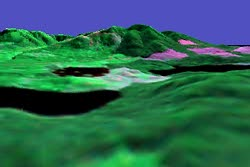
\includegraphics{images/sensores_remotos/canada/demview.jpg}

}

\caption{\label{fig-demview}Drapeado de imagen sobre elevación generando
perspectiva 3D. Fuente: CCRS/CCT ©}

\end{figure}%

Todas estas tecnologías forman el corazón de los \textbf{Sistemas de
Información Geográfica (SIG)}, estructurando el territorio en capas
temáticas para permitir modelamientos y toma de decisiones integrales.

\begin{figure}

\centering{

\includegraphics{images/sensores_remotos/canada/gis.gif}

}

\caption{\label{fig-gis}Modelo topológico de capas característico de un
SIG. Fuente: CCRS/CCT ©}

\end{figure}%

\chapter{Aplicaciones de los sensores
remotos}\label{aplicaciones-de-los-sensores-remotos}

\begin{quote}
\textbf{Fuente original:}
\href{https://natural-resources.canada.ca/science-data/science-research/geomatics/remote-sensing/tutorial-fundamentals-remote-sensing}{Natural
Resources Canada - Remote Sensing Tutorials}
\end{quote}

\section{Introducción a las
aplicaciones}\label{introducciuxf3n-a-las-aplicaciones}

El diseño de un sensor satelital o aéreo está dictado fundamentalmente
por su aplicación objetivo, lo que define sus parámetros de resolución
espacial, espectral, radiométrica y temporal.

Dado que la superficie terrestre es dinámica, a menudo un solo sensor no
puede satisfacer todas las necesidades analíticas. El paradigma actual
de la geomática se centra en la \textbf{integración} de datos,
utilizando técnicas complementarias: * \textbf{Multiespectral:}
Explotación de diversas bandas para generar firmas espectrales precisas.
* \textbf{Multisensor:} Combinación de tecnologías, como fusionar el
detalle topográfico/rugoso de un Radar de Apertura Sintética (SAR) con
la riqueza química y reflectiva de un sensor óptico. *
\textbf{Multitemporal:} Análisis de series de tiempo para derivar
variables de cambio, fenología o dinámica de desastres. Requiere el uso
estricto de datos calibrados radiométricamente.

\section{Agricultura}\label{agricultura}

La agricultura representa un pilar crítico en las economías globales. Su
rentabilidad y viabilidad exigen un flujo de información constante sobre
la salud de los cultivos, los rendimientos proyectados y las condiciones
edafológicas. La percepción remota es la única tecnología capaz de
proveer monitoreo sinóptico continuo desde la escala parcelaria hasta la
continental.

\begin{center}
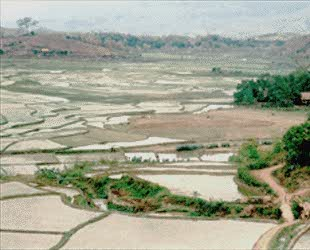
\includegraphics{images/sensores_remotos/canada/agric.jpg}
\end{center}
\begin{center}
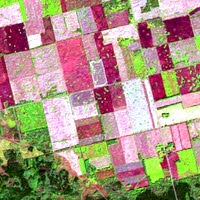
\includegraphics{images/sensores_remotos/canada/agrimag.jpg}
\end{center}

\subsection{Mapeo de tipos de
cultivos}\label{mapeo-de-tipos-de-cultivos}

La identificación del tipo de cultivo en áreas extensas es fundamental
para la gestión gubernamental y las proyecciones de mercado. Las
diferencias en la arquitectura de la planta y sus pigmentos permiten su
discriminación en el espectro visible e infrarrojo cercano.

Sin embargo, debido a que muchos cultivos pueden lucir espectralmente
idénticos en un momento dado, el mapeo se apoya fuertemente en
aproximaciones \textbf{multitemporales}. Al registrar la parcela en
múltiples fases de su ciclo fenológico (siembra, máximo verdor,
senescencia y cosecha), el algoritmo de clasificación puede aislar
especies basándose en su curva temporal de desarrollo. Asimismo, los
sensores de microondas (radar) asisten en el mapeo en zonas con alta
nubosidad al diferenciar la orientación de los surcos y la estructura
geométrica del dosel del cultivo.

\subsection{Monitoreo de condiciones y
rendimiento}\label{monitoreo-de-condiciones-y-rendimiento}

Una vez identificados los cultivos, es imperativo evaluar su vigor. El
estrés fisiológico (inducido por sequías, deficiencia de nutrientes,
malezas o infestación de plagas) se manifiesta frecuentemente como una
caída temprana en la reflectancia del infrarrojo cercano, antes de que
el daño sea visible al ojo humano en el espectro visible (clorosis).

La generación de Índices de Vegetación (como el NDVI) y el uso de
sensores térmicos para modelar el estrés hídrico permiten a los gestores
intervenir a tiempo mediante técnicas de \textbf{agricultura de
precisión}, focalizando la irrigación y el uso de agroquímicos,
maximizando así el rendimiento final de la cosecha.

\section{Silvicultura}\label{silvicultura}

Los ecosistemas forestales representan inmensos depósitos de
biodiversidad, sumideros de carbono y recursos maderables. Monitorear
áreas remotas o accidentadas requiere obligatoriamente observación
satelital y aerotransportada.

\subsection{Identificación de especies y
tipificación}\label{identificaciuxf3n-de-especies-y-tipificaciuxf3n}

La tipificación puede ir desde el reconocimiento regional de grandes
biomas hasta inventarios detallados a escala de rodal (altura, densidad,
biomasa). Las diferencias en la reflectancia foliar permiten separar
coníferas de bosques caducifolios.

Para estudios avanzados, el uso de datos \textbf{hiperespectrales}
ofrece un nivel de resolución sin precedentes. Permite cuantificar no
solo la especie, sino la densidad de los troncos y las anomalías
bioquímicas causadas por plagas. Por su parte, en biomas de nubosidad
perpetua (como las selvas tropicales), el Radar activo es la única
herramienta operativa confiable para mapear la degradación del dosel.

\begin{center}
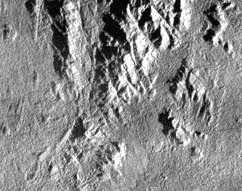
\includegraphics{images/sensores_remotos/canada/capsar.jpg}
\end{center}
\begin{center}
\includegraphics{images/sensores_remotos/canada/capmap.gif}
\end{center}

\begin{center}
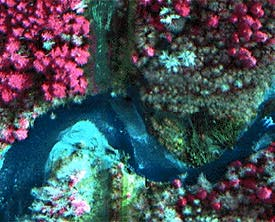
\includegraphics{images/sensores_remotos/canada/casiimag.jpg}
\end{center}
\begin{center}
\includegraphics{images/sensores_remotos/canada/casiistem.gif}
\end{center}
\begin{center}
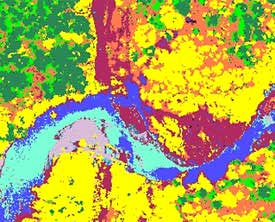
\includegraphics{images/sensores_remotos/canada/casiclas.jpg}
\end{center}

\begin{figure}

\centering{

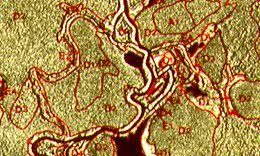
\includegraphics{images/sensores_remotos/canada/interp1.jpg}

}

\caption{\label{fig-interp1}Interpretación estructural del dosel
mediante datos SAR estereoscópicos. Fuente: CCRS/CCT ©}

\end{figure}%

\subsection{Mapeo de áreas quemadas}\label{mapeo-de-uxe1reas-quemadas}

El fuego es un agente de renovación, pero también de devastación. La
teledetección interviene mediante sensores térmicos para el monitoreo
logístico de incendios activos. Posteriormente, el mapeo de cicatrices
de quema en el espectro óptico permite evaluar el perímetro afectado y
la severidad del daño, información fundamental para estructurar planes
de mitigación de erosión y reforestación.

\begin{figure}

\centering{

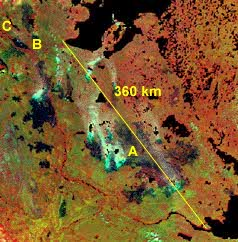
\includegraphics{images/sensores_remotos/canada/burn1a.jpg}

}

\caption{\label{fig-burn1a}Delineación térmica e infrarroja de un frente
de incendio en progreso. Fuente: CCRS/CCT ©}

\end{figure}%

\section{Geología}\label{geologuxeda}

La teledetección asiste a la exploración de hidrocarburos, la minería y
el análisis de riesgos geotécnicos mediante el estudio de la litología
superficial y la geomorfología.

\begin{figure}

\centering{

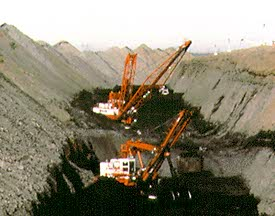
\includegraphics{images/sensores_remotos/canada/mine.jpg}

}

\caption{\label{fig-mine}Detección de yacimientos minerales y
alteraciones del terreno. Fuente: CCRS/CCT ©}

\end{figure}%

\subsection{Mapeo estructural y
topográfico}\label{mapeo-estructural-y-topogruxe1fico}

Las estructuras como fallas y pliegues rigen la dinámica del subsuelo.
El \textbf{Radar de Apertura Sintética (SAR)} domina este campo
analítico: su iluminación lateral controlada proyecta sombras
direccionales que maximizan relieves estructurales sutiles, revelando
lineamientos ocultos bajo densa vegetación.

\begin{center}
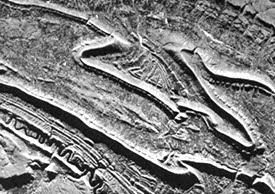
\includegraphics{images/sensores_remotos/canada/sarstruc.jpg}
\end{center}
\begin{center}
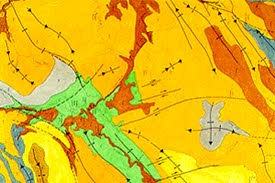
\includegraphics{images/sensores_remotos/canada/strucmap.jpg}
\end{center}
\begin{center}
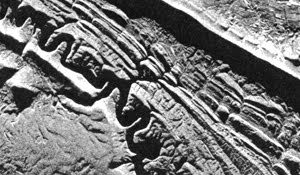
\includegraphics{images/sensores_remotos/canada/sarshad.jpg}
\end{center}

La integración de fisiografía SAR con geofísica aerotransportada (ej.
espectrometría de rayos gamma) permite un análisis multivariable
profundo de la geoquímica y la morfología del paisaje.

\begin{center}
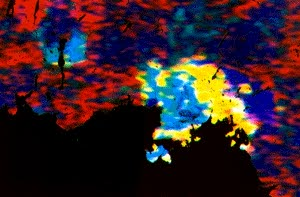
\includegraphics{images/sensores_remotos/canada/coldgamm.jpg}
\end{center}
\begin{center}
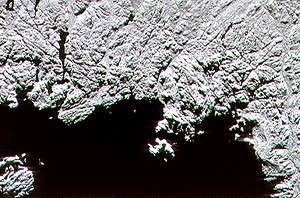
\includegraphics{images/sensores_remotos/canada/coldsar.jpg}
\end{center}
\begin{center}
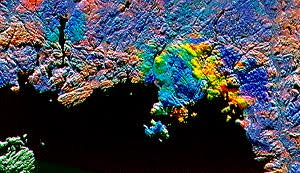
\includegraphics{images/sensores_remotos/canada/coldint.jpg}
\end{center}

\subsection{Mapeo de unidades
geológicas}\label{mapeo-de-unidades-geoluxf3gicas}

La delimitación de dominios litológicos se fundamenta en las variaciones
de reflectancia espectral (especialmente en el SWIR para detectar
arcillas y carbonatos) e integraciones con texturas radar, permitiendo
generar mapas precisos de la roca matriz.

\begin{center}
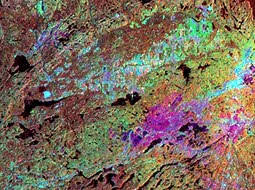
\includegraphics{images/sensores_remotos/canada/sudint.jpg}
\end{center}
\begin{center}
\includegraphics{images/sensores_remotos/canada/geomap.gif}
\end{center}

\section{Hidrología}\label{hidrologuxeda}

La geomática hidrológica monitorea los componentes del ciclo del agua,
desde cuencas y humedad de la biosfera, hasta la dinámica de cuerpos de
agua estacionarios.

\begin{figure}

\centering{

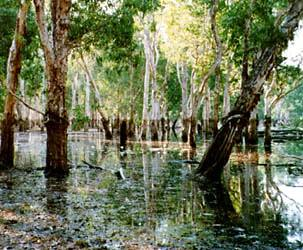
\includegraphics{images/sensores_remotos/canada/hyrdo.jpg}

}

\caption{\label{fig-hyrdo}Absorción casi total de energía infrarroja en
cuerpos de agua superficial. Fuente: CCRS/CCT ©}

\end{figure}%

\subsection{Humedad del suelo}\label{humedad-del-suelo}

La humedad del perfil superior del suelo controla el escurrimiento de la
precipitación y condiciona el crecimiento agrícola. A nivel remoto, se
aprovecha que la \textbf{constante dieléctrica} de los materiales
naturales responde drásticamente a la adición de agua. Los sensores
activos de microondas, al ser sensibles a las propiedades dieléctricas,
pueden cartografiar anomalías de saturación del suelo sin importar la
cobertura nubosa.

\begin{figure}

\centering{

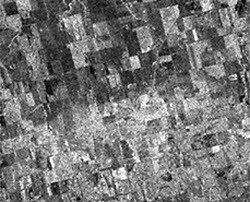
\includegraphics{images/sensores_remotos/canada/raindist.jpg}

}

\caption{\label{fig-raindist}Variación de la retrodispersión en función
de la humedad del suelo inducida por lluvias. Fuente: CCRS/CCT ©}

\end{figure}%

\subsection{Delineación y mapeo de
inundaciones}\label{delineaciuxf3n-y-mapeo-de-inundaciones}

Debido a que las inundaciones severas ocurren bajo cobertura nubosa
densa, los sensores ópticos suelen ser inoperantes. En emergencias, el
\textbf{SAR de microondas} (ej. RADARSAT) es fundamental: el agua
estancada actúa como un reflector especular (tono negro en la imagen),
generando un contraste extremo con la tierra seca circundante, lo que
permite delimitar la zona catastrófica en tiempo real.

\begin{center}
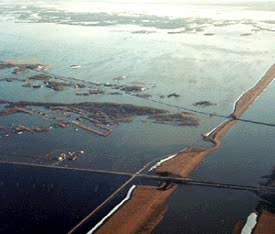
\includegraphics{images/sensores_remotos/canada/floodph1.jpg}
\end{center}
\begin{center}
\includegraphics{images/sensores_remotos/canada/noaflood.gif}
\end{center}
\begin{center}
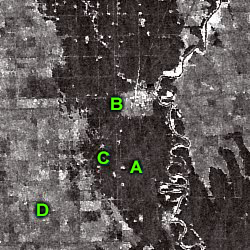
\includegraphics{images/sensores_remotos/canada/radflood.jpg}
\end{center}

\section{Hielo marino}\label{hielo-marino}

El monitoreo criosférico es indispensable para modelar el clima global y
garantizar la seguridad de la navegación comercial y exploración en
latitudes polares. Dada la oscuridad prolongada del invierno polar y las
persistentes nieblas, la teledetección operativa del hielo depende casi
exclusivamente de sensores de microondas y radar activo.

\subsection{Tipo de hielo y
concentración}\label{tipo-de-hielo-y-concentraciuxf3n}

Es vital discriminar entre hielo de primer año (frágil y delgado) y
hielo multianual (denso, grueso y peligroso para la navegación). Durante
el invierno, las salmueras atrapadas y la rugosidad superficial permiten
que el radar caracterice la edad y el grosor del paquete de hielo,
calculando automáticamente su nivel de concentración para trazar rutas
navegables seguras.

\begin{figure}

\centering{

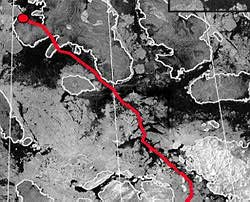
\includegraphics{images/sensores_remotos/canada/exped.jpg}

}

\caption{\label{fig-exped}Apoyo logístico a embarcaciones operando en
zonas de hielo denso. Fuente: CCRS/CCT ©}

\end{figure}%

\subsection{Dinámica y movimiento del
hielo}\label{dinuxe1mica-y-movimiento-del-hielo}

El hielo marino es una superficie altamente dinámica, movida por
corrientes oceánicas y vientos. Mediante la adquisición sistemática de
imágenes sobre una misma zona en ventanas de tiempo cortas
(multitemporalidad), los algoritmos de flujo óptico pueden rastrear el
desplazamiento de témpanos individuales, generando vectores de velocidad
y dirección del hielo, críticos para proteger plataformas de perforación
marina.

\section{Cobertura terrestre y uso del
suelo}\label{cobertura-terrestre-y-uso-del-suelo}

El mapeo de la cobertura terrestre sirve como inventario básico de los
recursos para los gobiernos y agencias ambientales. Permite capturar la
fenología de las plantas y realizar observaciones a escala regional y
continental.

\begin{figure}

\centering{

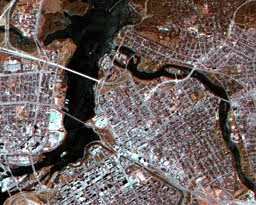
\includegraphics{images/sensores_remotos/canada/ottawa.jpg}

}

\caption{\label{fig-ottawa}Escena de Landsat TM de Ottawa, Ontario,
mostrando coberturas terrestres. Fuente: CCRS/CCT ©}

\end{figure}%

Para estudios regionales, la teledetección es la herramienta más
práctica y rentable, ya que proporciona información multiespectral,
multitemporal y \textbf{multisensor}. Integrar diferentes fuentes (como
datos ópticos TM con Radar SAR aerotransportado) aumenta
significativamente el contenido de información para una clasificación
precisa.

\begin{figure}

\centering{

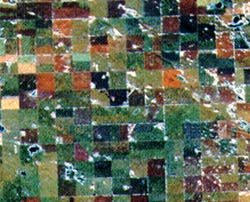
\includegraphics{images/sensores_remotos/canada/multisen.jpg}

}

\caption{\label{fig-multisen}Fusión multisensor (TM y SAR) para la
distinción de cultivos. Fuente: CCRS/CCT ©}

\end{figure}%

Mientras que los datos ópticos son ideales para la cartografía de la
cobertura, las imágenes de radar son un excelente sustituto en áreas con
alta nubosidad persistente, como las regiones tropicales.

\begin{figure}

\centering{

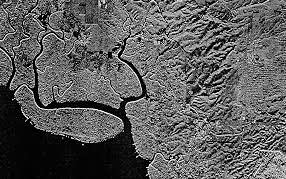
\includegraphics{images/sensores_remotos/canada/tawau4.jpg}

}

\caption{\label{fig-tawau4-lc}Imagen SAR mostrando la cobertura
terrestre tropical bajo nubes. Fuente: CCRS/CCT ©}

\end{figure}%

\subsection{Mapeo de biomasa y cobertura regional (Caso de estudio:
NBIOME)}\label{mapeo-de-biomasa-y-cobertura-regional-caso-de-estudio-nbiome}

Una iniciativa clave en el mapeo a gran escala es el desarrollo de
clasificaciones objetivas de los principales biomas, como el proyecto
NBIOME en Canadá. Este tipo de mapas base permite observar cambios en la
cobertura a lo largo del tiempo debido a factores climáticos o
antropogénicos.

\begin{figure}

\centering{

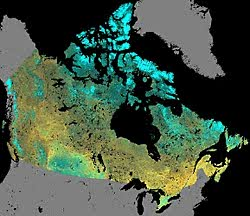
\includegraphics{images/sensores_remotos/canada/canmosi.jpg}

}

\caption{\label{fig-canmosi}Clasificación de la cobertura terrestre y
biomasa de Canadá. Fuente: CCRS/CCT ©}

\end{figure}%

Esta clasificación emplea datos de resolución moderada (1 km) del sensor
NOAA-AVHRR para garantizar un procesamiento eficiente. El método
consiste en crear \textbf{compuestos libres de nubes} de periodos de 10
días, seleccionando para cada píxel el valor con el Índice de Vegetación
de Diferencia Normalizada (NDVI) más alto (dado que un NDVI bajo indica
presencia de nubes).

Utilizando una metodología de ``clasificación por generalización
progresiva'' (que mezcla enfoques supervisados y no supervisados), los
algoritmos agrupan los datos en clústeres espectrales dominantes,
resultando en una cartografía de coberturas altamente objetiva y
reproducible a escala continental.

\subsection{Uso del suelo}\label{uso-del-suelo}

Aunque los términos suelen usarse indistintamente, representan conceptos
analíticos diferentes: la \textbf{cobertura terrestre} describe el
material biofísico sobre la superficie (bosque, asfalto, agua), mientras
que el \textbf{uso del suelo} refiere al propósito antropogénico
(recreacional, residencial, comercial).

\begin{figure}

\centering{

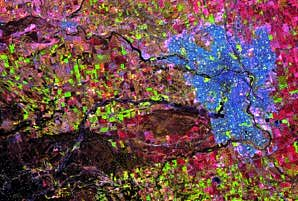
\includegraphics{images/sensores_remotos/canada/caltm.jpg}

}

\caption{\label{fig-caltm}Cartografía de coberturas del suelo sobre
bases multiespectrales (Landsat). Fuente: CCRS/CCT ©}

\end{figure}%

\subsection{Cambio de uso del suelo (Expansión
urbana)}\label{cambio-de-uso-del-suelo-expansiuxf3n-urbana}

A medida que las poblaciones aumentan, la periferia de las ciudades
experimenta una fuerte presión, transformando el paisaje de rural a
urbano. El monitoreo sistemático del sellado del suelo y el crecimiento
de infraestructuras es crucial para la planificación de servicios
públicos, estimación de recaudación fiscal y protección de fronteras
agrícolas. El fuerte retorno radiométrico de las geometrías urbanas
(rebote doble) facilita su identificación en imágenes SAR.

\begin{center}
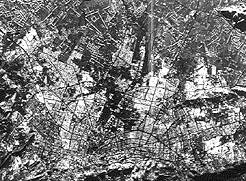
\includegraphics{images/sensores_remotos/canada/urbsar.jpg}
\end{center}
\begin{center}
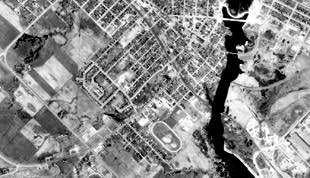
\includegraphics{images/sensores_remotos/canada/urbrural.jpg}
\end{center}

\section{Cartografía y
planimetría}\label{cartografuxeda-y-planimetruxeda}

La producción cartográfica es el producto base tradicional del análisis
espacial. Consiste en documentar topológicamente las infraestructuras,
hidrografía y límites administrativos, constituyendo el armazón sobre el
cual operan los Sistemas de Información Geográfica (SIG).

\begin{figure}

\centering{

\includegraphics{images/sensores_remotos/canada/mapping.gif}

}

\caption{\label{fig-mapping}Esquema del flujo geomático en la
actualización cartográfica. Fuente: CCRS/CCT ©}

\end{figure}%

\subsection{Planimetría}\label{planimetruxeda}

Se refiere a la extracción y geolocalización bidimensional (coordenadas
X, Y) de características del paisaje, como redes viales, polígonos
urbanos y redes de transmisión. Para que este proceso sea confiable y
alcance los estándares cartográficos nacionales, se exige imagery de
altísima resolución espacial y estrictos procesos de corrección
ortogonal.

\begin{center}
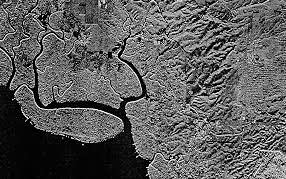
\includegraphics{images/sensores_remotos/canada/tawau4.jpg}
\end{center}
\begin{center}
\includegraphics{images/sensores_remotos/canada/tawau2.gif}
\end{center}

\subsection{Modelos Digitales de Elevación
(DEM)}\label{modelos-digitales-de-elevaciuxf3n-dem}

La inclusión de la tercera dimensión (Z) revoluciona la aplicabilidad de
los mapas bidimensionales, permitiendo correcciones de pendiente,
modelamiento hidrológico y vistas en perspectiva 3D.

Los DEM pueden extraerse mediante fotogrametría clásica (pares estéreo
ópticos) o, más eficientemente, utilizando tecnologías coherentes como
la \textbf{Interferometría Radar (InSAR)}. Esta técnica mide los
desfases ondulatorios entre dos adquisiciones radar ligeramente
separadas espacialmente, calculando el paralaje para derivar grillas
altimétricas continuas y de alta precisión sin necesidad de laboriosos
trabajos de campo.

\begin{center}
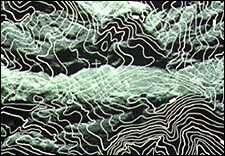
\includegraphics{images/sensores_remotos/canada/sarcontr.jpg}
\end{center}
\begin{center}
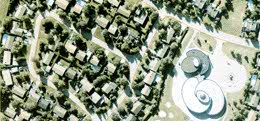
\includegraphics{images/sensores_remotos/canada/kanatdoi.jpg}
\end{center}

\subsection{Mapeo temático base (BTM)}\label{mapeo-temuxe1tico-base-btm}

El mapeo temático de línea base (Baseline Thematic Mapping) es la
integración digital avanzada de imágenes satelitales, métricas de uso
del suelo y datos topográficos para producir verdaderos ``mapas de
imágenes'' vectoriales.

\begin{figure}

\centering{

\includegraphics{images/sensores_remotos/canada/img2map.gif}

}

\caption{\label{fig-img2map}Esquema de integración conceptual en la
elaboración de BTM. Fuente: CCRS/CCT ©}

\end{figure}%

En este proceso analítico multivariable, la información óptica
multiespectral provee los límites planimétricos de la cobertura boscosa
o agrícola, mientras que la integración simultánea con Radar SAR aporta
la expresión geomorfológica tridimensional, consolidando una plataforma
integral idónea para la toma de decisiones en la asignación del uso del
territorio.

\section{Monitoreo oceánico y
costero}\label{monitoreo-oceuxe1nico-y-costero}

Los océanos cubren más de dos tercios de la superficie terrestre y son
el motor principal del sistema climático global. Asimismo, las zonas
costeras, que albergan a más del 60\% de la población mundial, son
ecosistemas biológicamente frágiles y sometidos a intenso estrés
antropogénico. La teledetección proporciona la escala sinóptica
necesaria para evaluar este vasto e inaccesible entorno.

\begin{figure}

\centering{

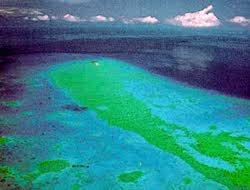
\includegraphics{images/sensores_remotos/canada/reef.jpg}

}

\caption{\label{fig-reef}Dinámica biológica en ecosistemas de arrecifes
costeros. Fuente: CCRS/CCT ©}

\end{figure}%

\subsection{Características oceánicas y
circulación}\label{caracteruxedsticas-oceuxe1nicas-y-circulaciuxf3n}

La comprensión de la dinámica oceánica permite optimizar las rutas de
navegación, modelar la dispersión de contaminantes y mejorar las
predicciones meteorológicas. Mediante sensores remotos es posible medir
la temperatura superficial del mar, la altura de las olas (altimetría) y
la dirección de los vientos (escaterometría).

El \textbf{Radar de Apertura Sintética (SAR)} es altamente efectivo para
este fin. Basado en el mecanismo de dispersión de \emph{Bragg}, el radar
detecta los patrones de rugosidad generados por las ondas capilares en
la interfase océano-atmósfera. Anomalías topográficas superficiales
sutiles revelan la presencia oculta de remolinos de mesoescala, frentes
y oscilaciones de marea internas.

\begin{figure}

\centering{

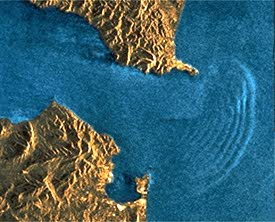
\includegraphics{images/sensores_remotos/canada/intwav.jpg}

}

\caption{\label{fig-intwav}Manifestación superficial de ondas internas
en el Estrecho de Gibraltar. Fuente: CCRS/CCT ©}

\end{figure}%

\subsection{Color del océano y concentración de
fitoplancton}\label{color-del-ocuxe9ano-y-concentraciuxf3n-de-fitoplancton}

El análisis del ``color del océano'' consiste en derivar parámetros
biológicos evaluando ópticamente las variaciones en la reflectancia de
la columna de agua. El fitoplancton marino, base de la red trófica,
depende del pigmento fotosintético de la clorofila para su
supervivencia. Esta molécula absorbe masivamente la luz en la región
roja y azul, confiriendo a las aguas productivas un fuerte tono verde
reflectivo.

Sensores especializados en bandas estrechas del espectro visible (como
SeaWiFS y MODIS) cuantifican estas concentraciones de clorofila. Esto
permite mapear la productividad primaria global, alertar sobre
floraciones algales nocivas, y comprender cómo perturbaciones climáticas
extremas ---como el desplazamiento de corrientes asociadas al evento de
El Niño--- destruyen temporalmente los reservorios pesqueros pelágicos.

\begin{figure}

\centering{

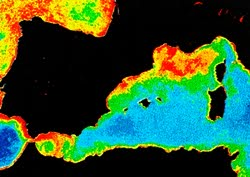
\includegraphics{images/sensores_remotos/canada/colormed.jpg}

}

\caption{\label{fig-colormed}Cartografía óptica multiespectral del nivel
de clorofila y actividad fitoplanctónica. Fuente: CCRS/CCT ©}

\end{figure}%

\subsection{Detección de derrames de
hidrocarburos}\label{detecciuxf3n-de-derrames-de-hidrocarburos}

Los vertidos de petróleo crudo en el mar resultan catastróficos para la
fauna marina y la economía litoral. Identificar el área inicial de un
derrame, modelar su dirección de arrastre y guiar las operaciones de
contención requieren una plataforma de vigilancia continua.

Si bien los fluorosensores láser aerotransportados ofrecen capacidades
químicas directas (``huella digital'' del hidrocarburo), los satélites
radar destacan operativamente al no depender de la luz diurna ni de
cielos despejados. Dado que la fina película de petróleo amortigua y
suaviza la tensión superficial del océano, elimina localmente las ondas
capilares generadas por el viento. Como resultado, el pulso del radar se
desvía de forma especular (alejándose de la antena), originando que la
región contaminada destaquen en la imagen radar como un polígono obscuro
de bordes claramente definidos contra la brillante retrodispersión del
mar circundante.

\begin{figure}

\centering{

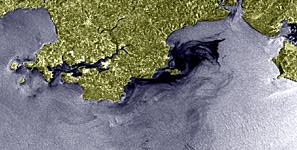
\includegraphics{images/sensores_remotos/canada/pollut.jpg}

}

\caption{\label{fig-pollut}Mancha oscura delineando la dispersión del
derrame del superpetrolero Sea Empress. Fuente: CCRS/CCT ©}

\end{figure}%

\chapter{Glosario de Sensores
Remotos}\label{glosario-de-sensores-remotos}

Términos y Definiciones

\hfill\break

\section{Referencias y Fuentes}\label{referencias-y-fuentes}

Este glosario ha sido compilado y adaptado utilizando material de las
siguientes fuentes de excelencia en observación de la Tierra:

\begin{itemize}
\tightlist
\item
  \textbf{NASA-ARSET}: Programa de Capacitación en Teledetección
  Aplicada de la NASA (Applied Remote Sensing Training).
\item
  \textbf{Natural Resources Canada}:
  \href{https://natural-resources.canada.ca/science-data/science-research/geomatics/remote-sensing/tutorial-fundamentals-remote-sensing}{Remote
  Sensing Tutorials - Fundamentals of Remote Sensing}.
\end{itemize}

\begin{center}\rule{0.5\linewidth}{0.5pt}\end{center}

\section{Requisitos de
finalización}\label{requisitos-de-finalizaciuxf3n}

Revisa los términos ordenados alfabéticamente a continuación para
conocer sus definiciones. Al terminar, haz clic en el botón de retroceso
de tu navegador para volver a la página principal del curso o utiliza el
menú de navegación para seleccionar la siguiente actividad.

\begin{center}\rule{0.5\linewidth}{0.5pt}\end{center}

\subsection{A}\label{a}

\begin{itemize}
\tightlist
\item
  \textbf{Absorción (Absorption):} Ocurre cuando la luz incidente golpea
  átomos y moléculas provocando que vibren.
\item
  \textbf{Albedo:} El albedo de una superficie es equivalente al
  porcentaje de reflectancia; es la fracción de radiación incidente que
  es reflejada por una superficie. Los valores van de 0 a 1, donde 0
  significa que la superficie absorbe toda la radiación y 1 significa
  que refleja toda la radiación.
\item
  \textbf{Amplitud (Amplitude):} La ``altura'' de una onda o su
  desplazamiento máximo desde el punto de equilibrio.
\item
  \textbf{Ancho de Barrido (Swath):} El área de la superficie de la
  Tierra capturada o escaneada durante una sola pasada de un avión o
  satélite.
\item
  \textbf{Ángulo de Incidencia (Incident Angle):} El ángulo formado
  entre un rayo incidente (por ejemplo, una onda de RADAR) sobre una
  superficie y la línea perpendicular a dicha superficie en el punto de
  incidencia.
\item
  \textbf{Antropogénico (Anthropogenic):} Resultante o derivado de la
  actividad humana.
\item
  \textbf{Aplicación (Application):} Se refiere a las preguntas o
  problemas del mundo real que los datos de teledetección ayudan a
  resolver. Los temas de aplicación incluyen calidad del aire,
  agricultura, gestión de desastres, manejo ecológico y ambiental, y
  calidad del agua.
\item
  \textbf{ARSET:} Programa de Capacitación en Teledetección Aplicada de
  la NASA (Applied Remote Sensing Training program).
\end{itemize}

\subsection{B}\label{b}

\begin{itemize}
\tightlist
\item
  \textbf{Banda (Band):} Representa un segmento seleccionado del
  espectro electromagnético. Típicamente, un instrumento de
  teledetección mide la radiación electromagnética en una o más bandas
  (ver \emph{Canal}).
\end{itemize}

\subsection{C}\label{c}

\begin{itemize}
\tightlist
\item
  \textbf{Canal (Channel):} Representa un segmento seleccionado del
  espectro electromagnético. Es un término que suele usarse de manera
  intercambiable con \emph{Banda}.
\item
  \textbf{Clasificación (Classification):} El proceso de utilizar
  ciertas características de los datos para asignar clases o categorías
  a áreas u objetos específicos. Categorizar cada píxel en una imagen
  como ``agua'' o ``tierra'' es un ejemplo de clasificación.
\item
  \textbf{Composición de Imagen en Color Verdadero (True Color Imagery
  Composite):} Una combinación de bandas que muestra a la Tierra en
  colores similares a los que veríamos con nuestros propios ojos. Los
  colores de visualización rojo, verde y azul se asignan a las
  longitudes de onda visibles roja, verde y azul, respectivamente.
\item
  \textbf{Composición de Imagen en Falso Color (False Color Imagery
  Composite / RGB):} Una composición que asigna los colores de
  visualización rojo, verde y azul (RGB) a longitudes de onda que no
  corresponden necesariamente a los colores rojo, verde y azul del
  espectro visible.
\item
  \textbf{Cuadriculado / En grilla (Gridded):} Datos espaciales
  organizados sobre una cuadrícula uniforme y espacialmente referenciada
  (por ejemplo, una cuadrícula de latitud y longitud).
\end{itemize}

\subsection{D}\label{d}

\begin{itemize}
\tightlist
\item
  \textbf{DAAC:} Centro de Archivo Activo Distribuido (Distributive
  Active Archive Center); los datos de la NASA se archivan en varios
  DAACs.
\item
  \textbf{Detección y Medición por Luz (LiDAR - Light Detection and
  Ranging):} Una técnica de teledetección activa que funciona bajo el
  mismo principio que el radar, pero utiliza luz de un láser en lugar de
  ondas de radio.
\item
  \textbf{Dispersión (Scattering):} Redirección de la radiación
  electromagnética a través de interacciones con partículas o moléculas
  en la atmósfera.
\end{itemize}

\subsection{E}\label{e}

\begin{itemize}
\tightlist
\item
  \textbf{Emisión (Emission):} Ocurre cuando un objeto libera radiación
  electromagnética a partir de su propia energía.
\item
  \textbf{Energía Electromagnética (Electromagnetic Energy):} Energía
  que viaja en forma de ondas y abarca el espectro electromagnético,
  como la proveniente del sol. La cantidad de energía transmitida varía
  con la longitud de onda.
\item
  \textbf{Energía Solar (Solar Energy):} La energía electromagnética
  emitida por el sol, también conocida como radiación solar.
\item
  \textbf{Enmascaramiento (Masking):} Un método para eliminar ciertas
  secciones de una imagen (por ejemplo, remover nubes para dejar solo la
  porción utilizable de los datos).
\item
  \textbf{ESA:} Agencia Espacial Europea (European Space Agency).
\item
  \textbf{Espectro Electromagnético (Electromagnetic Spectrum):} Término
  utilizado para describir el rango completo de las longitudes de onda
  de la radiación electromagnética. Incluye rayos gamma, rayos X, luz
  ultravioleta, luz visible, infrarrojos, microondas y ondas de radio.
\item
  \textbf{Espectrometría (Spectrometry):} La ciencia de estudiar e
  identificar la materia en función de cómo interactúa con la radiación
  electromagnética.
\item
  \textbf{Espectrómetro (Spectrometer):} Un sensor utilizado para medir
  las propiedades de la luz en las regiones ultravioleta, visible e
  infrarrojo cercano del espectro electromagnético.
\item
  \textbf{Espectrorradiómetro (Spectroradiometer):} Un sensor que mide
  tanto la longitud de onda como la amplitud de la luz emitida.
\item
  \textbf{Extensión Espacial (Spatial Extent):} El área superficial
  total cubierta por un conjunto de datos (dataset) determinado.
\end{itemize}

\subsection{F}\label{f}

\begin{itemize}
\tightlist
\item
  \textbf{Fase (Phase):} La posición de un punto en el tiempo dentro de
  un ciclo de forma de onda.
\item
  \textbf{Firma Espectral (Spectral signature):} La respuesta espectral
  de una superficie u objeto; es la forma en que el material responde a
  la radiación incidente en función de la longitud de onda.
\item
  \textbf{Frecuencia (Frequency):} El número de ciclos de una onda que
  pasan por un punto fijo por unidad de tiempo.
\end{itemize}

\subsection{G}\label{g}

\begin{itemize}
\tightlist
\item
  \textbf{Geoestacionario (Geostationary):} Que permanece fijo sobre una
  ubicación específica en la superficie de la Tierra (acompañando la
  rotación terrestre).
\item
  \textbf{Georreferenciación (Georeference):} El acto de vincular datos
  espaciales a su ubicación correcta sobre, debajo o por encima de la
  superficie de la Tierra.
\end{itemize}

\subsection{I}\label{i}

\begin{itemize}
\tightlist
\item
  \textbf{Imágenes Hiperespectrales (Hyperspectral Imaging):} Medición a
  través del espectro electromagnético utilizando cientos o miles de
  bandas muy estrechas.
\item
  \textbf{In Situ:} Término que significa ``en el lugar original''. En
  teledetección, se refiere comúnmente a los datos recopilados en el
  terreno para validar los datos capturados por sensores remotos aéreos
  o espaciales.
\item
  \textbf{Infrarrojo (Infrared):} Una región de longitudes de onda en el
  espectro electromagnético, de 0.75 a 100 µm (\(7.5 \times 10^{-7}\) -
  \(10^{-4}\) m).
\item
  \textbf{Infrarrojo Cercano (NIR - Near Infrared):} Una subregión de la
  zona infrarroja del espectro electromagnético, con longitudes de onda
  de 0.75 a 1.4 µm (\(7.5 \times 10^{-7}\) - \(1.4 \times 10^{-6}\) m).
\item
  \textbf{Infrarrojo de Onda Corta (SWIR - Shortwave Infrared):} Una
  subregión infrarroja del espectro electromagnético, con longitudes de
  onda de 1.4 a 4 µm (\(1.4 \times 10^{-6}\) - \(3 \times 10^{-6}\) m).
\item
  \textbf{Infrarrojo de Onda Larga (LWIR - Longwave Infrared):} Una
  subregión infrarroja del espectro electromagnético, con longitudes de
  onda de 8 a 15 µm (\(8 \times 10^{-6}\) - \(1.5 \times 10^{-5}\) m).
\item
  \textbf{Infrarrojo Térmico (TIR - Thermal Infrared):} Una subregión
  infrarroja del espectro electromagnético (8 a 15 µm) donde los objetos
  emiten radiación en función de su temperatura. El TIR es crucial para
  estudiar las temperaturas de la superficie y la atmósfera.
\item
  \textbf{Intensidad (Intensity):} La transferencia de potencia promedio
  durante un período de la onda. Es proporcional al cuadrado de la
  amplitud de la onda.
\end{itemize}

\subsection{L}\label{l}

\begin{itemize}
\tightlist
\item
  \textbf{Longitud de Onda (Wavelength):} La distancia desde la cresta
  de una onda hasta la siguiente; la longitud de onda es inversamente
  proporcional a la frecuencia.
\item
  \textbf{Luz Visible (Visible light):} La región del espectro
  electromagnético que es visible para el ojo humano y contiene los
  colores del arco iris, con longitudes de onda de 750 nm a 400 nm (rojo
  \textasciitilde690nm, verde \textasciitilde530nm, azul
  \textasciitilde420nm).
\end{itemize}

\subsection{M}\label{m}

\begin{itemize}
\tightlist
\item
  \textbf{Microondas (Microwave):} Una región de longitudes de onda en
  el espectro electromagnético, desde 1 mm (\(10^{-3}\) m) hasta 100 mm
  (\(10^{-1}\) m).
\item
  \textbf{Multiespectral (Multispectral):} Medición a través del
  espectro electromagnético utilizando generalmente entre 3 y 10 bandas.
\end{itemize}

\subsection{N}\label{n}

\begin{itemize}
\tightlist
\item
  \textbf{Nadir:} El punto en la superficie de la Tierra directamente
  debajo del satélite de observación.
\item
  \textbf{NASA:} Administración Nacional de Aeronáutica y el Espacio
  (National Aeronautics and Space Administration).
\item
  \textbf{NOAA:} Oficina Nacional de Administración Oceánica y
  Atmosférica (National Oceanic and Atmospheric Administration).
\end{itemize}

\subsection{O}\label{o}

\begin{itemize}
\tightlist
\item
  \textbf{Observaciones de la Tierra (Earth Observations):} Información
  sobre los sistemas físicos, químicos y biológicos de la Tierra (por
  ejemplo, imágenes satelitales).
\item
  \textbf{Ondas de Radio (Radio waves):} La región con las longitudes de
  onda más largas en el espectro electromagnético, desde 1 m hasta 100
  km (1 - \(10^5\) m).
\item
  \textbf{Ondas de Rayos Gamma (Gamma ray waves):} La región con las
  longitudes de onda más cortas en el espectro electromagnético, desde 1
  fm (\(10^{-15}\) m) hasta 100 fm (\(10^{-13}\) m).
\item
  \textbf{Ondas de Rayos X (X-Ray waves):} Una región de longitudes de
  onda en el espectro electromagnético, desde 1 pm (\(10^{-12}\) m)
  hasta 100 pm (\(10^{-10}\) m).
\item
  \textbf{Ondas Ultravioleta / UV (Ultraviolet waves):} Una región de
  longitudes de onda en el espectro electromagnético, de 100 nm
  (\(10^{-7}\) m) a 1 nm (\(10^{-9}\) m).
\item
  \textbf{Óptico (Optical):} Sensores que recopilan luz de las partes
  visibles e infrarrojas del espectro.
\item
  \textbf{Órbita Polar (Polar Orbit):} Un tipo de órbita que cruza en o
  cerca de los polos Norte y Sur.
\end{itemize}

\subsection{P}\label{p}

\begin{itemize}
\tightlist
\item
  \textbf{Parámetro Geofísico (Geophysical parameter):} Propiedades
  medibles dentro del sistema terrestre. La temperatura de la superficie
  terrestre, la humedad en el aire y la altura de los árboles son
  ejemplos de parámetros geofísicos.
\item
  \textbf{Plataforma (Platform):} Lo que transporta a un sensor.
  Generalmente, un satélite o un avión.
\item
  \textbf{Polarímetro (Polarimeter):} Un sensor que mide la intensidad y
  la orientación de las ondas de luz.
\item
  \textbf{Polarización (Polarization):} La orientación o alineación de
  una onda electromagnética.
\item
  \textbf{Porcentaje de Reflectancia (Percent Reflectance):} La relación
  entre la energía reflejada y la energía total incidente sobre el
  objeto a una longitud de onda dada.
\item
  \textbf{Proyección (Projection):} Los medios por los cuales se muestra
  un sistema de coordenadas y datos espaciales en una superficie plana.
\end{itemize}

\subsection{R}\label{r}

\begin{itemize}
\tightlist
\item
  \textbf{Radar:} Un sensor activo que utiliza ondas de radio para medir
  la distancia a un objeto.
\item
  \textbf{Radar de Apertura Sintética (SAR - Synthetic Aperture Radar):}
  Una forma de radar que utiliza el movimiento de la antena para crear
  una resolución espacial más fina (detallada) que un radar estacionario
  tradicional.
\item
  \textbf{Radar Polarimétrico (Polarimetric radar):} Un sensor que
  produce su propia energía de microondas y mide tanto la intensidad de
  la energía que regresa al satélite como la orientación de la onda
  electromagnética en sí.
\item
  \textbf{Radiación de Onda Corta (Shortwave radiation):} Se refiere a
  la porción del espectro electromagnético emitida por el sol con
  longitudes de onda entre 0.1 µm y 4 µm, que incluye las regiones
  ultravioleta, visible e infrarroja.
\item
  \textbf{Radiación Electromagnética (Electromagnetic Radiation):}
  Energía que viaja en forma de ondas. Es un término intercambiable con
  \emph{Energía Electromagnética}.
\item
  \textbf{Radiación Incidente (Incident Radiation):} La energía
  electromagnética entrante que golpea una superficie.
\item
  \textbf{Radiación Solar (Solar Radiation):} La energía
  electromagnética emitida por el sol.
\item
  \textbf{Radiancia (Radiance):} Una medida de la potencia de la
  radiación electromagnética emitida desde un objeto objetivo por unidad
  de área para una longitud de onda determinada. En el espectro visible,
  también se describe como el brillo de la fuente en una dirección dada.
\item
  \textbf{Radiómetro de imágenes (Imaging radiometer):} Mide la cantidad
  de energía reflejada y emitida en porciones específicas del Espectro
  Electromagnético.
\item
  \textbf{Radiómetro de microondas (Microwave radiometer):} Un sensor
  que mide varias bandas de microondas diferentes dentro del espectro
  electromagnético.
\item
  \textbf{Recuperación / Extracción (Retrieval):} El proceso de utilizar
  datos brutos de un sensor remoto (es decir, medidas de radiación) para
  cuantificar un parámetro geofísico.
\item
  \textbf{Reflectancia (Reflectance):} Una medida de la luz o el calor
  reflejado por un objeto objetivo.
\item
  \textbf{Reflexión (Reflection):} Las ondas electromagnéticas que
  rebotan en una superficie en un ángulo igual y opuesto al ángulo de la
  radiación incidente.
\item
  \textbf{Resolución Espacial (Spatial Resolution):} El tamaño de un
  píxel dentro de una imagen digital y el área real en la superficie de
  la Tierra representada por ese píxel.
\item
  \textbf{Resolución Espectral (Spectral Resolution):} La capacidad de
  un sensor para diferenciar entre longitudes de onda. A mayor
  resolución espectral, más estrecho es el rango de longitud de onda
  para un canal o banda dada.
\item
  \textbf{Resolución Radiométrica (Radiometric Resolution):} La
  precisión de un sensor para detectar diferencias en la intensidad de
  la señal, expresada frecuentemente en bits (por ejemplo, 8 bits o 16
  bits).
\item
  \textbf{Resolución Temporal (Temporal Resolution):} El intervalo de
  tiempo en el que un sensor mide u observa la misma ubicación (tiempo
  de revisita).
\item
  \textbf{Retrodispersión (Backscatter):} Se refiere a la energía
  reflejada directamente de regreso hacia su fuente después de golpear
  un objetivo (muy utilizado en RADAR).
\end{itemize}

\subsection{S}\label{s}

\begin{itemize}
\tightlist
\item
  \textbf{Satélite (Satellite):} Una nave espacial que orbita la Tierra
  y proporciona una plataforma para instrumentos científicos, incluidos
  los sensores remotos.
\item
  \textbf{Sensor (Sensor):} Un instrumento montado en una plataforma que
  detecta y mide la radiación reflejada o emitida por los objetos. El
  término ``instrumento'' se usa de manera intercambiable.
\item
  \textbf{Sensor Activo (Active Sensor):} Un sensor que proporciona su
  propia iluminación o energía y mide lo que se refleja de regreso (ej.
  RADAR o LiDAR).
\item
  \textbf{Sensor Pasivo (Passive Sensor):} Un sensor que no proporciona
  su propia iluminación, sino que mide la energía reflejada o emitida
  que proviene de fuentes naturales (como el sol).
\item
  \textbf{Series de Tiempo (Time Series):} Una serie de imágenes sobre
  una misma área objetivo recopiladas en diferentes puntos en el tiempo.
\item
  \textbf{SIG (GIS):} Sistema de Información Geográfica (Geographic
  Information System).
\item
  \textbf{Sincronizado con el Sol / Heliosíncrono (Sun-Synchronous):} Un
  tipo de órbita donde el satélite está sincronizado con la relación
  espacial entre la Tierra y el Sol, lo que significa que siempre pasa
  sobre el mismo lugar a la misma hora solar local.
\end{itemize}

\subsection{T}\label{t}

\begin{itemize}
\tightlist
\item
  \textbf{Teledetección / Percepción Remota (Remote Sensing):} El
  proceso de recopilar información sobre objetos desde la distancia, sin
  estar en contacto físico con ellos.
\item
  \textbf{Teledetección Aerotransportada (Airborne Remote Sensing):}
  Instrumentos de teledetección montados en aviones o vehículos aéreos
  no tripulados (UAV / Drones) para recopilar datos.
\item
  \textbf{Transmisión (Transmission):} Ocurre cuando un objeto es
  transparente a ciertas longitudes de onda de la radiación incidente y
  les permite pasar a su través.
\end{itemize}

\subsection{U}\label{u}

\begin{itemize}
\tightlist
\item
  \textbf{USGS:} Servicio Geológico de los Estados Unidos (United States
  Geological Survey).
\end{itemize}

\subsection{V}\label{v}

\begin{itemize}
\tightlist
\item
  \textbf{Ventana Atmosférica (Atmospheric Window):} Una región en el
  espectro electromagnético donde la atmósfera terrestre es
  relativamente transparente, permitiendo que la radiación pase con una
  absorción o dispersión mínima.
\end{itemize}

\chapter{Recursos Adicionales de
Teledetección}\label{recursos-adicionales-de-teledetecciuxf3n}

Fundamentos de Sensores Remotos

\hfill\break

\section{Requisitos de
finalización}\label{requisitos-de-finalizaciuxf3n-1}

A continuación, se presenta una lista de herramientas, portales y
documentos recomendados para complementar y profundizar tu aprendizaje
sobre la teledetección satelital y la observación de la Tierra.

\begin{center}\rule{0.5\linewidth}{0.5pt}\end{center}

\subsection{Módulo 1: ¿Por qué Observaciones de la Tierra
(EO)?}\label{muxf3dulo-1-por-quuxe9-observaciones-de-la-tierra-eo}

\begin{itemize}
\tightlist
\item
  \href{https://science.nasa.gov/earth-science/missions/}{Sitio de
  Misiones de Ciencias de la Tierra de la NASA}
\item
  \href{https://space.oscar.wmo.int/satellites}{Lista de Satélites OSCAR
  de la Organización Meteorológica Mundial (OMM)}
\item
  \href{https://eo4society.esa.int/communities/users/}{Áreas Temáticas
  de Observación de la Tierra para Usuarios Públicos y Privados por la
  ESA}
\end{itemize}

\subsection{Módulo 2: ¿Qué es la
Teledetección?}\label{muxf3dulo-2-quuxe9-es-la-teledetecciuxf3n}

\begin{itemize}
\tightlist
\item
  \href{https://smd-cms.nasa.gov/wp-content/uploads/2023/08/tour-of-the-ems-tagged-v7-0.pdf}{Tour
  del Espectro Electromagnético}
\item
  \href{https://science.nasa.gov/ems/01_intro}{NASA Science -
  Introducción al Espectro Electromagnético}
\item
  \href{https://eo4society.esa.int/}{Ciencia Abierta de Observación de
  la Tierra de la Agencia Espacial Europea (ESA)} - Materiales
  educativos y capacitación sobre observación de la Tierra.
\item
  \href{https://www.nesdis.noaa.gov/}{Servicio de Información y
  Satélites de la NOAA (NESDIS)} - Explica cómo los satélites de la NOAA
  observan la Tierra, con módulos de capacitación para principiantes.
\end{itemize}

\subsection{Módulo 3: ¿Cómo Funciona la
Teledetección?}\label{muxf3dulo-3-cuxf3mo-funciona-la-teledetecciuxf3n}

\begin{itemize}
\tightlist
\item
  \href{https://earthobservatory.nasa.gov/features/RemoteSensing/remote_08.php}{Métodos
  de Teledetección del NASA Earth Observatory}
\item
  \href{https://www.esa.int/Enabling_Support/Space_Transportation/Types_of_orbits\#GEO}{ESA
  -- Tipos de Órbitas}
\item
  \href{https://www.earthdata.nasa.gov/learn/earth-observation-data-basics/remote-sensing}{NASA
  Earth Data -- Aprender \textgreater{} Conceptos Básicos de Datos de
  Observación de la Tierra \textgreater{} Teledetección}
\item
  \href{https://natural-resources.canada.ca/maps-tools-and-publications/satellite-imagery-elevation-data-and-air-photos/tutorial-fundamentals-remote-sensing/9309}{Centro
  Canadiense de Teledetección (CCRS) - Tutorial de Fundamentos de
  Teledetección}
\end{itemize}

\subsection{Módulo 4: ¿Cómo Uso los Datos de
Teledetección?}\label{muxf3dulo-4-cuxf3mo-uso-los-datos-de-teledetecciuxf3n}

\begin{itemize}
\tightlist
\item
  \href{https://appliedsciences.nasa.gov/get-involved/training}{Catálogo
  de Capacitación en Ciencias Aplicadas de NASA/ARSET}
\item
  \href{https://www.earthdata.nasa.gov/learn/pathfinders}{Earthdata
  Pathfinders (Guías de Ruta de Datos de la Tierra)}
\item
  \href{https://www.earthdata.nasa.gov/data/instruments}{Instrumentos de
  Earth Data}
\item
  \href{https://www.earthdata.nasa.gov/engage/open-data-services-and-software/data-and-information-policy/data-levels}{NASA
  Earthdata -- Niveles de Procesamiento de Datos}
\item
  \href{https://earthobservatory.nasa.gov/features/FalseColor}{NASA
  Earth Observatory -- ¿Por qué ese Bosque es Rojo y esa Nube es Azul?}
\item
  \href{https://www.meted.ucar.edu/education_training/lessons/568}{COMET/MetEd
  - Aplicaciones Satelitales Multiespectrales: Explicación de Productos
  RGB}
\item
  \href{https://earthobservatory.nasa.gov/features/ColorImage}{NASA
  Earth Observatory - Cómo Interpretar una Imagen Satelital, 5 Consejos}
\item
  \href{https://science.nasa.gov/ems/04_energytoimage/}{NASA Science --
  Visualización: De Energía a Imagen}
\item
  \href{https://eros.usgs.gov/}{Centro de Ciencia y Observación de
  Recursos Terrestres (EROS) del USGS} - Tutoriales y herramientas para
  aplicar datos de Landsat y otros datos de teledetección.
\item
  \href{https://www.opendatacube.org/}{Open Data Cube} - Proporciona
  tutoriales sobre cómo acceder y analizar imágenes satelitales de
  varios sensores.
\item
  \href{https://dataspace.copernicus.eu/}{Copernicus Data Space
  Ecosystem} - Ayuda a los usuarios a acceder y analizar los datos de
  los satélites Sentinel de la Unión Europea.
\end{itemize}

\part{Prácticas}

\chapter{Visualización y Mapas Dinámicos}\label{sec-viz}

\section{Introducción}\label{introducciuxf3n-1}

En la Geomática moderna, la capacidad de comunicar resultados mediante
mapas interactivos y salidas gráficas de alta calidad es fundamental.
Gracias a iniciativas como \textbf{OpenGeos} y el ecosistema de
\textbf{R-Spatial}, hoy podemos generar productos cartográficos
profesionales con muy pocas líneas de código.

\section{Visualización Interactiva (Web
Maps)}\label{visualizaciuxf3n-interactiva-web-maps}

Los mapas dinámicos permiten explorar datos espaciales con zoom y
desplazamiento, facilitando la validación de información en tiempo real.

\subsection{🐍 Python (Leafmap \& Geemap)}

En Python, utilizamos \texttt{leafmap} para datos vectoriales y
\texttt{geemap} para el procesamiento masivo en la nube con Google Earth
Engine.

Documentación de \texttt{leafmap}
\href{https://github.com/opengeos/leafmap}{aquí!}

\begin{Shaded}
\begin{Highlighting}[]
\ImportTok{import}\NormalTok{ leafmap}

\CommentTok{\# 1. Crear el objeto mapa centrado en el Ecuador con zoom global}
\CommentTok{\# Leafmap permite usar diversos mapas base por defecto}
\NormalTok{m }\OperatorTok{=}\NormalTok{ leafmap.Map(center}\OperatorTok{=}\NormalTok{[}\DecValTok{0}\NormalTok{, }\DecValTok{0}\NormalTok{], zoom}\OperatorTok{=}\DecValTok{2}\NormalTok{)}

\CommentTok{\# 2. Definir la ruta del archivo GeoJSON (Cables submarinos)}
\CommentTok{\# Se utiliza una URL de release para mayor compatibilidad con los drivers GDAL}
\NormalTok{in\_geojson }\OperatorTok{=}\NormalTok{ (}
    \StringTok{"https://github.com/opengeos/datasets/releases/download/vector/cables.geojson"}
\NormalTok{)}

\CommentTok{\# 3. Añadir la capa al mapa con un nombre específico}
\CommentTok{\# Este método lee el archivo remoto y lo renderiza sobre el mapa base}
\NormalTok{m.add\_geojson(in\_geojson, layer\_name}\OperatorTok{=}\StringTok{"Líneas de Cable"}\NormalTok{)}

\CommentTok{\# 4. Mostrar el mapa interactivo}
\NormalTok{m}
\end{Highlighting}
\end{Shaded}

Documentación de \texttt{geemap}
\href{https://github.com/gee-community/geemap}{aquí!}

\begin{Shaded}
\begin{Highlighting}[]
\ImportTok{import}\NormalTok{ geemap}

\CommentTok{\# 1. Crear el mapa centrado en un punto (Bogotá) para evitar errores de geometría}
\NormalTok{m }\OperatorTok{=}\NormalTok{ geemap.Map(center}\OperatorTok{=}\NormalTok{[}\FloatTok{4.63}\NormalTok{, }\OperatorTok{{-}}\FloatTok{74.08}\NormalTok{], zoom}\OperatorTok{=}\DecValTok{10}\NormalTok{)}

\CommentTok{\# 2. Cargar colección Sentinel{-}2 Armonizada (ID corArecto para 2024)}
\NormalTok{collection }\OperatorTok{=}\NormalTok{ (}
\NormalTok{    geemap.ee.ImageCollection(}\StringTok{\textquotesingle{}COPERNICUS/S2\_SR\_HARMONIZED\textquotesingle{}}\NormalTok{)}
\NormalTok{    .filterDate(}\StringTok{\textquotesingle{}2024{-}01{-}01\textquotesingle{}}\NormalTok{, }\StringTok{\textquotesingle{}2024{-}03{-}31\textquotesingle{}}\NormalTok{)}
\NormalTok{    .median()}
\NormalTok{)}

\CommentTok{\# 3. Parámetros de visualización simples}
\NormalTok{vis\_params }\OperatorTok{=}\NormalTok{ \{}\StringTok{\textquotesingle{}min\textquotesingle{}}\NormalTok{: }\DecValTok{0}\NormalTok{, }\StringTok{\textquotesingle{}max\textquotesingle{}}\NormalTok{: }\DecValTok{3000}\NormalTok{, }\StringTok{\textquotesingle{}bands\textquotesingle{}}\NormalTok{: [}\StringTok{\textquotesingle{}B4\textquotesingle{}}\NormalTok{, }\StringTok{\textquotesingle{}B3\textquotesingle{}}\NormalTok{, }\StringTok{\textquotesingle{}B2\textquotesingle{}}\NormalTok{]\}}

\CommentTok{\# 4. Añadir capa y mostrar}
\NormalTok{m.addLayer(collection, vis\_params, }\StringTok{\textquotesingle{}Sentinel{-}2 UNAL\textquotesingle{}}\NormalTok{)}
\NormalTok{m}
\end{Highlighting}
\end{Shaded}

\subsection{🏁 R (Mapview)}

En R, \texttt{mapview} ofrece una solución de una sola línea para
visualizar objetos espaciales de forma interactiva.

Documentación sobre \texttt{mapview}
\href{https://r-spatial.github.io/mapview/}{aquí!}

\begin{Shaded}
\begin{Highlighting}[]
\FunctionTok{library}\NormalTok{(sf)}
\FunctionTok{library}\NormalTok{(mapview)}

\CommentTok{\# 1. Crear punto de referencia UNAL Bogotá (EPSG:4326)}
\NormalTok{unal }\OtherTok{\textless{}{-}} \FunctionTok{st\_sfc}\NormalTok{(}\FunctionTok{st\_point}\NormalTok{(}\FunctionTok{c}\NormalTok{(}\SpecialCharTok{{-}}\FloatTok{74.08}\NormalTok{, }\FloatTok{4.63}\NormalTok{)), }\AttributeTok{crs =} \DecValTok{4326}\NormalTok{)}

\CommentTok{\# 2. Visualización interactiva inmediata}
\CommentTok{\# Genera automáticamente controles de capas y mapas base}
\FunctionTok{mapview}\NormalTok{(unal, }\AttributeTok{col.regions =} \StringTok{"red"}\NormalTok{, }\AttributeTok{layer.name =} \StringTok{"Sede Bogotá"}\NormalTok{)}
\end{Highlighting}
\end{Shaded}

\section{Visualización Estática (Mapas para
Publicación)}\label{visualizaciuxf3n-estuxe1tica-mapas-para-publicaciuxf3n}

Para reportes profesionales o artículos científicos, se requiere un
control total sobre la estética, escalas y grillas.

\subsection{🐍 Python (Geopandas + Matplotlib)}

\texttt{Geopandas} es una herramienta que une el análisis de datos
tradicional en python (\texttt{pandas}) con la cartografía,
permitiéndote manipular formas geométricas con la misma facilidad con la
que manipulas columnas en una hoja de Excel. Geopandas usa por debajo la
librería \texttt{matplotlib} para hacer los mapas estáticos y
\texttt{leaflet} para los dinámicos.

Documentación sobre \texttt{geopandas}
\href{https://geopandas.org/en/stable/}{aquí!}

\begin{Shaded}
\begin{Highlighting}[]
\CommentTok{\# Instala la librería geodatasets.}
\CommentTok{\#!pip3 install geodatasets}

\CommentTok{\# Importa geopandas y geodatasets.}
\ImportTok{import}\NormalTok{ geopandas}
\ImportTok{from}\NormalTok{ geodatasets }\ImportTok{import}\NormalTok{ get\_path}

\CommentTok{\# Obtiene la ruta del dataset:}
\CommentTok{\# "nybb" (New York Borough Boundaries).}
\NormalTok{path\_to\_data }\OperatorTok{=}\NormalTok{ get\_path(}\StringTok{"nybb"}\NormalTok{)}

\CommentTok{\# Lee el archivo y lo convierte }
\CommentTok{\# en un GeoDataFrame}
\NormalTok{gdf }\OperatorTok{=}\NormalTok{ geopandas.read\_file(path\_to\_data)}

\CommentTok{\# Muestra la tabla.}
\NormalTok{gdf}

\CommentTok{\# {-}{-}{-} Visualización Estática {-}{-}{-}}
\CommentTok{\# Genera un mapa fijo usando Matplotlib, coloreando por el nombre del distrito.}
\CommentTok{\# Se incluye una leyenda para identificar cada color con su respectivo \textquotesingle{}Borough\textquotesingle{}.}
\NormalTok{gdf.plot(}\StringTok{"BoroName"}\NormalTok{, legend}\OperatorTok{=}\VariableTok{True}\NormalTok{)}

\CommentTok{\# {-}{-}{-} Visualización Dinámica {-}{-}{-}}
\CommentTok{\# Crea un mapa interactivo basado en Leaflet.}
\CommentTok{\# El mapa base se carga automáticamente.}
\NormalTok{gdf.explore(}\StringTok{"BoroName"}\NormalTok{, legend}\OperatorTok{=}\VariableTok{False}\NormalTok{)}
\end{Highlighting}
\end{Shaded}

\subsection{🏁 R (Tmap \& Ggplot2)}

\texttt{tmap} permite una gramática puramente cartográfica, mientras que
\texttt{ggplot2} integra el mapa en flujos de trabajo estadísticos.

Documentación sobre \texttt{tmap}
\href{https://r-tmap.github.io/tmap/}{aquí!}

Documentación sobre \texttt{ggplot2} + \texttt{sf}
\href{https://ggplot2.tidyverse.org/reference/ggsf.html}{aquí!}

\begin{Shaded}
\begin{Highlighting}[]
\CommentTok{\# \#| eval: false}
\FunctionTok{library}\NormalTok{(sf)}
\end{Highlighting}
\end{Shaded}

\begin{verbatim}
Linking to GEOS 3.12.1, GDAL 3.8.4, PROJ 9.4.0; sf_use_s2() is TRUE
\end{verbatim}

\begin{Shaded}
\begin{Highlighting}[]
\FunctionTok{library}\NormalTok{(tmap)}
\FunctionTok{library}\NormalTok{(ggplot2)}

\CommentTok{\# {-}{-}{-} Usando tmap (Ideal para cartografía temática) {-}{-}{-}}
\FunctionTok{data}\NormalTok{(}\StringTok{"World"}\NormalTok{)}
\NormalTok{col }\OtherTok{\textless{}{-}}\NormalTok{ World[World}\SpecialCharTok{$}\NormalTok{name }\SpecialCharTok{==} \StringTok{"Colombia"}\NormalTok{, ]}

\FunctionTok{tm\_shape}\NormalTok{(col) }\SpecialCharTok{+}
  \FunctionTok{tm\_polygons}\NormalTok{(}\StringTok{"pop\_est"}\NormalTok{, }\AttributeTok{palette =} \StringTok{"Blues"}\NormalTok{, }\AttributeTok{title =} \StringTok{"Población Est."}\NormalTok{) }\SpecialCharTok{+}
  \FunctionTok{tm\_compass}\NormalTok{(}\AttributeTok{position =} \FunctionTok{c}\NormalTok{(}\StringTok{"right"}\NormalTok{, }\StringTok{"top"}\NormalTok{)) }\SpecialCharTok{+}
  \FunctionTok{tm\_scale\_bar}\NormalTok{()}
\end{Highlighting}
\end{Shaded}

\begin{verbatim}
\end{verbatim}

\begin{verbatim}
-- tmap v3 code detected -------------------------------------------------------
\end{verbatim}

\begin{verbatim}
[v3->v4] `tm_tm_polygons()`: migrate the argument(s) related to the scale of
the visual variable `fill` namely 'palette' (rename to 'values') to fill.scale
= tm_scale(<HERE>).
[v3->v4] `tm_polygons()`: migrate the argument(s) related to the legend of the
visual variable `fill` namely 'title' to 'fill.legend = tm_legend(<HERE>)'
! `tm_scale_bar()` is deprecated. Please use `tm_scalebar()` instead.
The visual variable `fill` of the layer "polygons" contains a unique value.
Therefore a discrete scale is applied (tm_scale_discrete).
[cols4all] color palettes: use palettes from the R package cols4all. Run
`cols4all::c4a_gui()` to explore them. The old palette name "Blues" is named
"brewer.blues"
Multiple palettes called "blues" found: "brewer.blues", "matplotlib.blues". The first one, "brewer.blues", is returned.
\end{verbatim}


\includegraphics{41-practica_1_clase2_visualizacion_dinamica_files/figure-pdf/tmap_ggplot2_r-1.pdf}

\begin{Shaded}
\begin{Highlighting}[]
\CommentTok{\# {-}{-}{-} Usando ggplot2 (Gramática de gráficos) {-}{-}{-}}
\FunctionTok{ggplot}\NormalTok{() }\SpecialCharTok{+}
  \FunctionTok{geom\_sf}\NormalTok{(}\AttributeTok{data =}\NormalTok{ col, }\AttributeTok{fill =} \StringTok{"orange"}\NormalTok{, }\AttributeTok{color =} \StringTok{"black"}\NormalTok{) }\SpecialCharTok{+}
  \FunctionTok{theme\_minimal}\NormalTok{() }\SpecialCharTok{+}
  \FunctionTok{labs}\NormalTok{(}\AttributeTok{title =} \StringTok{"Mapa de Colombia con ggplot2"}\NormalTok{)}
\end{Highlighting}
\end{Shaded}


\includegraphics{41-practica_1_clase2_visualizacion_dinamica_files/figure-pdf/tmap_ggplot2_r-2.pdf}

\begin{center}\rule{0.5\linewidth}{0.5pt}\end{center}

\subsection{Notas de Reproducibilidad}\label{notas-de-reproducibilidad}

\begin{itemize}
\tightlist
\item
  \textbf{Persistencia}: Recuerde trabajar siempre dentro de
  \texttt{/home/rstudio/work} para que sus scripts no se borren al
  reiniciar el contenedor.
\item
  \textbf{Red}: La visualización de capas remotas requiere conexión a
  internet estable dentro del entorno Docker.
\item
  \textbf{Motores}: Todo el renderizado depende de las librerías de
  sistema GDAL, GEOS y PROJ preinstaladas.
\end{itemize}

\begin{tcolorbox}[enhanced jigsaw, opacityback=0, left=2mm, colbacktitle=quarto-callout-note-color!10!white, leftrule=.75mm, breakable, titlerule=0mm, rightrule=.15mm, bottomrule=.15mm, arc=.35mm, colback=white, colframe=quarto-callout-note-color-frame, opacitybacktitle=0.6, toptitle=1mm, title=\textcolor{quarto-callout-note-color}{\faInfo}\hspace{0.5em}{Ejercicio}, bottomtitle=1mm, toprule=.15mm, coltitle=black]

Intente cargar un archivo vectorial local desde su carpeta de trabajo y
visualícelo usando \texttt{mapview} en R o \texttt{m.add\_gdf()} en
Python.

\end{tcolorbox}

\section{🏁 Desafío de Laboratorio: Visualización
Geoespacial}\label{desafuxedo-de-laboratorio-visualizaciuxf3n-geoespacial}

Este laboratorio busca consolidar el manejo de las herramientas de
Jupyter Lab y VSCode usando lenguaje Quarto. Adicionalmente es una
introducción rápica a la creación de mapas estáticos y dinámicos y su
exportación a formato HTML. La geomática es la ciencia de gestionar
información geográfica mediante mapas digitales y análisis de datos. Si
hay una frase que describe a la geomática, es la creación y análisis de
mapas digitales. El objetivo es que el estudiante valide el
funcionamiento de algunos de los entornos de trabajo instalados.

\begin{center}\rule{0.5\linewidth}{0.5pt}\end{center}

\subsection{🛠️ Instrucciones de Entrega}\label{instrucciones-de-entrega}

\begin{enumerate}
\def\labelenumi{\arabic{enumi}.}
\tightlist
\item
  Creen un nuevo repositorio en su \textbf{GitHub personal} llamado
  \texttt{taller1-sig-visualizacion}.
\item
  Todas las respuestas escritas deben estar en un archivo
  \texttt{respuestas.qmd}.
\item
  Rendericen \texttt{respuestas.qmd} a \textbf{HTML} y \textbf{PDF}.
\item
  Suban al repositorio los \textbf{4 notebooks} solicitados y los
  archivos de Quarto.
\end{enumerate}

\begin{center}\rule{0.5\linewidth}{0.5pt}\end{center}

\subsection{⚙️ Parte A --- Notebooks de Clase
(Reproducibilidad)}\label{parte-a-notebooks-de-clase-reproducibilidad}

Creen cuatro notebooks donde ejecuten \textbf{exactamente} el código
desarrollado en clase. Esto asegura que su entorno (Docker/Jupyter) está
correctamente configurado.

\subsubsection{📒 Notebooks Obligatorios:}\label{notebooks-obligatorios}

\begin{enumerate}
\def\labelenumi{\arabic{enumi}.}
\tightlist
\item
  \textbf{\texttt{01\_python\_estatico.ipynb}}: Código de
  \texttt{geopandas} + \texttt{geodatasets} para graficar los distritos
  de Nueva York (\texttt{nybb}) usando \texttt{.plot()}.
\item
  \textbf{\texttt{02\_python\_dinamico.ipynb}}: Código de
  \texttt{leafmap} cargando el GeoJSON de cables submarinos y el código
  de \texttt{geemap} con Sentinel-2 Armonizada.
\item
  \textbf{\texttt{03\_r\_estatico.ipynb}}: Código de \texttt{sf} +
  \texttt{tmap} mostrando el mapa de población de Colombia con brújula y
  escala.
\item
  \textbf{\texttt{04\_r\_dinamico.ipynb}}: Código de \texttt{mapview}
  mostrando el punto de la Sede Bogotá con la configuración para
  notebooks.
\end{enumerate}

\begin{quote}
Seguramente no podrá visualizar algunos de esos resultados usando
Notebooks, como alternativa tiene VSCode y los archivos Quarto (pero
esto es opcional)
\end{quote}

\begin{center}\rule{0.5\linewidth}{0.5pt}\end{center}

\subsection{🖥️ Parte B --- Desafío de
Exploración}\label{parte-b-desafuxedo-de-exploraciuxf3n}

En su archivo \texttt{respuestas.qmd}, elijan \textbf{una} de las
siguientes librerías de Python (OpenGeos) y creen un nuevo bloque de
código que demuestre una funcionalidad \textbf{diferente} a la vista en
clase, guiándose por su documentación oficial:

\begin{itemize}
\tightlist
\item
  \textbf{Leafmap}: Implementar un mapa de pantalla dividida
  (\texttt{split-panel}) o un inspector de atributos.
\item
  \textbf{Geemap}: Cargar un dataset diferente (ej. elevación SRTM o uso
  de suelo ESA WorldCover).
\item
  \textbf{Mapwidget}: Crear un mapa utilizando un motor diferente como
  \texttt{Cesium} o \texttt{MapLibre}.
  \href{https://github.com/opengeos/mapwidget}{Documentación}
\item
  \textbf{Anymap-ts}:
  \href{https://github.com/opengeos/anymap-ts}{Documentación.}
\item
  \textbf{Anymap-ts}:
  \href{https://github.com/opengeos/anymap}{Documentación.}
\end{itemize}

\begin{center}\rule{0.5\linewidth}{0.5pt}\end{center}

\subsection{\texorpdfstring{❓ Preguntas de Análisis para
\texttt{respuestas.qmd}}{❓ Preguntas de Análisis para respuestas.qmd}}\label{preguntas-de-anuxe1lisis-para-respuestas.qmd}

\subsubsection{1. 🥇 Facilidad e
Intuición}\label{facilidad-e-intuiciuxf3n}

Basado en los 4 notebooks de clase: ¿Cuál de las librerías les pareció
más intuitiva para un usuario que nunca ha programado?

\subsubsection{2. 🎨 Calidad
Cartográfica}\label{calidad-cartogruxe1fica}

Para la entrega de un informe técnico en PDF, ¿qué motor consideran que
genera mapas estáticos con mejor acabado visual: \texttt{tmap},
\texttt{matplotlib} (\texttt{geopandas.plot}), \texttt{ggplot2}?

\subsubsection{3. 🌐 Potencial de la
Documentación}\label{potencial-de-la-documentaciuxf3n}

Al revisar las URL de documentación entregadas, ¿qué funcionalidad
avanzada encontraron en el ecosistema de \textbf{OpenGeos} que les sería
útil para su trabajo final o investigación?

\subsubsection{4. 🧠 Elección de
Herramientas}\label{elecciuxf3n-de-herramientas}

Si tuvieran que atender una emergencia ambiental real y necesitan
desplegar un visor web en menos de 5 minutos para que personal no
técnico visualice una inundación, ¿qué herramienta elegirían y por qué?
(Máximo 5 líneas).

\begin{center}\rule{0.5\linewidth}{0.5pt}\end{center}

\begin{quote}
💡 \textbf{Nota para el éxito}

La precisión en la ruta de los datos y el manejo de los kernels es
fundamental. Si un mapa dinámico no carga, revise los mensajes de la
consola de Quarto para descartar problemas de rutas de JavaScript. Y
utilice IA para encontrar soluciones!
\end{quote}

\chapter{🌐 Geoportales y Servicios Web}\label{sec-geoportales-intro}

\section{📖 Introducción a los Datos
Abiertos}\label{sec-geoportales-datos-abiertos}

En la Geomática moderna, la tendencia es el \textbf{consumo de servicios
web}. Esto garantiza trabajar con información oficial y actualizada sin
saturar el almacenamiento local. Según el enfoque de \textbf{Open
Science}, es vital usar herramientas que permitan la reproducibilidad y
el acceso libre a la información, evitando el almacenamiento aislado en
discos duros locales.

Para esta sesión, utilizaremos como guía técnica los recursos de
\textbf{Rodolfo Franco}:

\begin{itemize}
\tightlist
\item
  🔗 \textbf{Geoservicios en Colombia:}
  \href{https://rodolfofrancoweb.com/geodata/geoservicios-colombia/}{rodolfofrancoweb.com/geodata/geoservicios-colombia/}
\item
  🔗 \textbf{Geoportales y Datos Abiertos:}
  \href{https://rodolfofrancoweb.com/sig/geoportales_datos_abiertos_e_ides/geoservicios/}{rodolfofrancoweb.com/sig/geoportales\_datos\_abiertos\_e\_ides/geoservicios/}
\end{itemize}

\begin{center}\rule{0.5\linewidth}{0.5pt}\end{center}

\section{📂 Formatos de Datos
Comunes}\label{sec-geoportales-formatos-descrip}

Además del acceso a servicios, los Geoportales permiten la descarga de
archivos físicos para procesamiento local. Es vital distinguir entre las
estructuras de los modelos de datos.

\subsection{📍 Comparativa de Formatos
Vectoriales}\label{comparativa-de-formatos-vectoriales}

Representan la realidad mediante puntos, líneas y polígonos asociados a
una tabla de atributos.

\begin{longtable}[]{@{}
  >{\raggedright\arraybackslash}p{(\columnwidth - 6\tabcolsep) * \real{0.1552}}
  >{\raggedright\arraybackslash}p{(\columnwidth - 6\tabcolsep) * \real{0.1034}}
  >{\raggedright\arraybackslash}p{(\columnwidth - 6\tabcolsep) * \real{0.4483}}
  >{\raggedright\arraybackslash}p{(\columnwidth - 6\tabcolsep) * \real{0.2931}}@{}}
\toprule\noalign{}
\begin{minipage}[b]{\linewidth}\raggedright
Formato
\end{minipage} & \begin{minipage}[b]{\linewidth}\raggedright
Tipo
\end{minipage} & \begin{minipage}[b]{\linewidth}\raggedright
Características Técnicas
\end{minipage} & \begin{minipage}[b]{\linewidth}\raggedright
Uso Recomendado
\end{minipage} \\
\midrule\noalign{}
\endhead
\bottomrule\noalign{}
\endlastfoot
\textbf{GeoPackage (.gpkg)} & Vector/Raster & Estándar abierto basado en
SQLite. Almacena múltiples capas en \textbf{un solo archivo}. &
\textbf{El estándar moderno.} Recomendado para QGIS y ArcGIS Pro. \\
\textbf{Shapefile (.shp)} & Vector & Formato ``multi-archivo'' (mínimo
\texttt{.shp}, \texttt{.shx}, \texttt{.dbf}). Límite de 2GB y nombres
cortos. & Uso legado. Muy común pero técnicamente limitado. \\
\textbf{GeoJSON (.geojson)} & Vector & Formato basado en texto (JSON).
Ligero y legible para humanos. & Visualización web y programación. \\
\textbf{File Geodatabase (.gdb)} & Vector/Raster & Formato propietario
de ESRI. Estructura de carpetas optimizada. & Proyectos complejos dentro
del ecosistema ArcGIS. \\
\end{longtable}

\subsection{🗺️ Comparativa de Formatos
Raster}\label{comparativa-de-formatos-raster}

Representan la realidad mediante una cuadrícula de celdas o píxeles
(elevación, reflectancia, etc.).

\begin{longtable}[]{@{}
  >{\raggedright\arraybackslash}p{(\columnwidth - 6\tabcolsep) * \real{0.1552}}
  >{\raggedright\arraybackslash}p{(\columnwidth - 6\tabcolsep) * \real{0.1034}}
  >{\raggedright\arraybackslash}p{(\columnwidth - 6\tabcolsep) * \real{0.4483}}
  >{\raggedright\arraybackslash}p{(\columnwidth - 6\tabcolsep) * \real{0.2931}}@{}}
\toprule\noalign{}
\begin{minipage}[b]{\linewidth}\raggedright
Formato
\end{minipage} & \begin{minipage}[b]{\linewidth}\raggedright
Tipo
\end{minipage} & \begin{minipage}[b]{\linewidth}\raggedright
Características Técnicas
\end{minipage} & \begin{minipage}[b]{\linewidth}\raggedright
Uso Recomendado
\end{minipage} \\
\midrule\noalign{}
\endhead
\bottomrule\noalign{}
\endlastfoot
\textbf{GeoTIFF (.tif)} & Raster & Archivo TIFF con georreferenciación.
Soporta múltiples bandas. & \textbf{Estándar universal} para imágenes y
MDE. \\
\textbf{Cloud Optimized GeoTIFF (COG)} & Raster & Diseñado para lectura
eficiente desde servidores en la nube sin descarga completa. & Análisis
masivo en la nube (Google Earth Engine). \\
\textbf{ASCII Grid (.asc)} & Raster & Formato de texto simple. Fácil de
leer pero ineficiente. & Intercambio con software de modelado
antiguo. \\
\end{longtable}

\begin{center}\rule{0.5\linewidth}{0.5pt}\end{center}

\section{🛠️ Estándares de Interoperabilidad
OGC}\label{sec-geoportales-ogc-detallado}

La \textbf{Open Geospatial Consortium (OGC)} establece estándares para
que la información geográfica sea intercambiable entre diferentes
plataformas.

\subsection{Principales Servicios Web
Geográficos}\label{principales-servicios-web-geogruxe1ficos}

\begin{itemize}
\tightlist
\item
  🖼️ \textbf{WMS (Web Map Service):} Transmite \textbf{mapas
  renderizados} como imágenes. No permite editar ni realizar cálculos
  sobre los valores originales.
\item
  📐 \textbf{WFS (Web Feature Service):} Entrega \textbf{entidades
  vectoriales} con geometría y atributos. Permite análisis espacial y
  cambio de simbología local.
\item
  🏔️ \textbf{WCS (Web Coverage Service):} Entrega \textbf{coberturas
  raster} con valores científicos originales. Indispensable para
  análisis con MDE.
\item
  ⚡ \textbf{WMTS (Web Map Tile Service):} Basado en \textbf{teselas
  (tiles)} pre-generadas. Extremadamente rápido para navegación web.
\end{itemize}

\begin{center}\rule{0.5\linewidth}{0.5pt}\end{center}

\section{📍 Introducción a Sistemas de
Coordenadas}\label{sec-geoportales-coordenadas}

\subsection{Coordenadas Geográficas
vs.~Planas}\label{sec-geoportales-tipos-coords}

\begin{itemize}
\tightlist
\item
  🌍 \textbf{Sistemas Geográficos:} Expresan la posición en grados sobre
  un elipsoide. Ejemplo: \textbf{WGS84 (EPSG: 4326)}.
\item
  📐 \textbf{Sistemas Planos (Proyectados):} Proyectan la curvatura
  terrestre sobre un plano usando metros. Permiten cálculos de área y
  distancia precisos.
\end{itemize}

\subsection{🇨🇴 El Contexto en
Colombia}\label{sec-geoportales-coordenadas-col}

\begin{enumerate}
\def\labelenumi{\arabic{enumi}.}
\tightlist
\item
  ⏳ \textbf{Orígenes Anteriores (MAGNA-SIRGAS):} Se utilizaban 5
  orígenes (Bogotá, Este, Este-Este, Oeste y Oeste-Oeste). Antes existía
  el sistema ARENA.
\item
  🎯 \textbf{Origen Nacional Único (EPSG: 9377):} Estándar actual.
  Unifica todo el país en un solo origen central para evitar rupturas de
  coordenadas.
\item
  🏢 \textbf{Orígenes Locales:} Ciudades como Bogotá o Medellín
  mantienen parámetros específicos para obras de alta precisión local.
\end{enumerate}

\subsection{🚀 Proyección ``al vuelo''
(On-the-fly)}\label{sec-geoportales-otf}

Tanto en QGIS como en ArcGIS Pro, el software realiza una
\textbf{proyección al vuelo} para que datos en diferentes sistemas
coincidan visualmente en pantalla sin alterar los archivos originales.

\begin{center}\rule{0.5\linewidth}{0.5pt}\end{center}

\section{📝 Práctica: Conexión y
Navegación}\label{sec-geoportales-paso-paso}

\textbf{Objetivo:} Integrar datos locales y servicios remotos para
validar la interoperabilidad de la información geográfica colombiana.

\subsection{📤 Entregable}\label{entregable}

Cargar en GitHub un archivo \textbf{QMD} (renderizado en \textbf{HTML} y
\textbf{PDF}) con:

\begin{enumerate}
\def\labelenumi{\arabic{enumi}.}
\tightlist
\item
  \textbf{Tabla de Fuentes:} Detalle de URL, nombre de archivo local y
  sistema de coordenadas (debe incluir 1 WMS, 1 WFS, 1 WCS, 1 Shapefile
  y 1 GeoTIFF).
\item
  \textbf{Productos Cartográficos:} Dos mapas en PDF (uno de QGIS y otro
  de ArcGIS Pro).
\end{enumerate}

\subsection{❓ Cuestionario de
Análisis}\label{cuestionario-de-anuxe1lisis}

\begin{itemize}
\tightlist
\item
  ¿Qué archivos/servicios permiten la edición de geometrías
  directamente?
\item
  ¿Cuáles permiten acceso a la tabla de atributos? Describa tres campos
  de uno de ellos.
\item
  ¿En qué casos fue posible cambiar la simbología desde el software
  cliente?
\item
  ¿Por qué es preferible usar un \textbf{WFS} sobre un
  \textbf{Shapefile} descargado en proyectos a largo plazo?
\end{itemize}

\begin{center}\rule{0.5\linewidth}{0.5pt}\end{center}

\section{👥 Modalidad de Trabajo}\label{sec-geoportales-modalidad}

\begin{itemize}
\tightlist
\item
  👤 \textbf{Tipo de actividad:} Individual.
\item
  🤝 \textbf{Colaboración:} Se fomenta el apoyo mutuo en la búsqueda de
  URLs y errores, pero los productos digitales y el análisis deben ser
  de autoría propia.
\end{itemize}

\chapter{Sistemas de Coordenadas - ArcGIS
Pro}\label{sistemas-de-coordenadas---arcgis-pro}

\begin{itemize}
\tightlist
\item
  Guía: ./docs/``03 t Coordenadas ArcGIS.pdf''
\item
  Datos: ./docs/coordenadas.zip
\item
  Documentos:

  \begin{itemize}
  \tightlist
  \item
    ./docs/coordenadas\_colombia.pdf
  \item
    ./docs/``documentos\_parametros oficiales.pdf''
  \end{itemize}
\end{itemize}

\chapter{Conversión de Formatos (ArcGIS Pro -
QGIS)}\label{conversiuxf3n-de-formatos-arcgis-pro---qgis}

\href{https://drive.google.com/file/d/1ZhzEN-3Cg7yP-lbsST7zk-mEq4IKvUO4/view?usp=sharing}{👉
Descargar Datos del Taller de Conversión (incluye datos para ejercicios
finales)}

\section{Introducción}\label{introducciuxf3n-2}

Establecer estándares universales para datos geográficos ha demostrado
ser un objetivo complejo. En la actualidad, no existe una normalización
única que tenga aceptación global absoluta, en parte por la continua
evolución tecnológica y por los ecosistemas cerrados que han
desarrollado diversos fabricantes de software a lo largo del tiempo.

Sin embargo, frente a la necesidad de compartir datos, la tendencia se
ha enfocado en el uso y creación de formatos de intercambio (o el
soporte multipropósito mediante librerías como GDAL/OGR) que permiten
trasladar información de un sistema a otro, evitando la pérdida de datos
o la duplicación de esfuerzos técnicos. Un usuario moderno de Sistemas
de Información Geográfica (SIG) debe conocer los métodos y las
herramientas para convertir datos espaciales a formatos compatibles
según la necesidad de análisis o la plataforma de trabajo (ArcGIS Pro,
QGIS, bases de datos espaciales, etc.).

\section{Objetivos}\label{objetivos}

\begin{itemize}
\tightlist
\item
  Reconocer los diversos formatos de estructuras de datos vectoriales y
  ráster soportados por los SIG modernos.
\item
  Comprender los fundamentos teóricos detrás de la compresión de
  imágenes y las reglas de asignación espacial durante las
  transformaciones.
\item
  Practicar los métodos de importación, exportación e intercambio de
  diferentes formatos de datos espaciales en ArcGIS Pro y QGIS.
\item
  Ejecutar conversiones geográficas de datos ráster a vector y de vector
  a ráster.
\end{itemize}

\section{Marco de referencia}\label{marco-de-referencia}

Cuando se habla de conversión de formatos, se hace referencia a dos
dimensiones distintas: por un lado, la migración de archivos entre
diferentes extensiones o arquitecturas (ej. de Shapefile a GeoPackage)
y, por otro, la conversión del modelo de datos espaciales, es decir, de
vector a ráster (rasterización) o de ráster a vector (vectorización).

\subsection{Consideraciones sobre formatos vectoriales y
CAD}\label{consideraciones-sobre-formatos-vectoriales-y-cad}

Muchos de los datos que se incorporan a los SIG provienen de programas
de Dibujo Asistido por Computador (CAD). Existe una gran variedad de
formatos CAD, siendo los más comunes como estándar de intercambio los
\texttt{.dxf} y \texttt{.dwg} (AutoCAD) y los \texttt{.dgn}
(MicroStation).

Estos archivos suelen almacenar la información de las entidades
separándolas gráficamente en puntos, líneas, polígonos y anotaciones
(textos). Al incorporarlos a un SIG, es importante recordar que a menudo
carecen de un sistema de coordenadas espaciales definido (proyección
geométrica pura), por lo que suele ser necesario georreferenciarlos y
exportarlos a formatos nativos SIG (como Geodatabases o GeoPackages)
para habilitar su análisis topológico y de atributos.

\subsection{Consideraciones sobre formatos ráster y
compresión}\label{consideraciones-sobre-formatos-ruxe1ster-y-compresiuxf3n}

El conocimiento de la procedencia y las características de cada formato
de imagen permite su óptima utilización. Algunos de los más relevantes
incluyen:

\begin{itemize}
\tightlist
\item
  \textbf{Multibandas nativos (.BIL, .BIP, .BSQ):} Formatos binarios
  clásicos utilizados para almacenar información satelital original.
  Suelen requerir archivos de texto adjuntos (metadatos o archivos
  \emph{world}) que le indican al software el orden de los bytes y las
  coordenadas de georreferenciación.
\item
  \textbf{ERDAS IMAGINE (.IMG):} Diseñado para almacenar tanto rásters
  de capas temáticas (usos del suelo discretos) como variables continuas
  (imágenes satelitales, Modelos Digitales de Terreno).
\item
  \textbf{TIFF / GeoTIFF (.TIF):} Uno de los formatos más extendidos por
  su flexibilidad. El estándar GeoTIFF permite incrustar etiquetas
  (tags) en la cabecera del archivo con la información de proyección,
  datum, elipsoide y coordenadas, evitando la necesidad de archivos de
  referenciación externos.
\end{itemize}

\textbf{Los formatos de compresión:} Existen básicamente dos formas de
comprimir documentos ráster: 1. \textbf{Con pérdida de información
(Lossy):} Como \textbf{JPEG} o \textbf{MrSID} (Multiresolution Seamless
Image Database). Alcanzan proporciones de compresión altísimas (20:1 o
más) transformando o desechando valores redundantes. Son excelentes para
visualización de fondos (ortofotos), pero \textbf{no se recomiendan para
procesos de análisis digital} ya que alteran los valores originales de
los píxeles. 2. \textbf{Sin pérdida de información (Lossless):} Como
\textbf{LZW} o \textbf{Run-Length Encoding (RLE)}. Reducen el tamaño del
archivo agrupando valores idénticos sin alterar los datos crudos, siendo
ideales para preservar la integridad analítica de la imagen.

\subsection{Operaciones de conversión de capas vectoriales a ráster y
viceversa}\label{operaciones-de-conversiuxf3n-de-capas-vectoriales-a-ruxe1ster-y-viceversa}

Las conversiones de modelos de datos responden a reglas geométricas
estrictas para decidir cómo se asignan los valores en el espacio.

\textbf{De Vectorial a Ráster (Rasterización):} El proceso superpone una
retícula ortogonal sobre la capa vectorial. Cada píxel toma un valor
numérico heredado de un campo de la tabla de atributos del vector
original. Las reglas de asignación suelen ser:

\begin{itemize}
\tightlist
\item
  \textbf{Polígonos:} El píxel toma el valor del polígono que coincide
  con su centroide, o aquel que cubre la mayor área de la celda.
\item
  \textbf{Líneas:} El píxel toma el valor de la línea que lo intersecta.
  Si varias líneas lo cruzan, toma el valor de la primera detectada o se
  pueden aplicar reglas de prioridad.
\item
  \textbf{Puntos:} El píxel adquiere el valor del punto contenido en él.
  \emph{(Nota: Si un píxel no coincide con ningún objeto, se le asigna
  valor ``No Data'' o nulo).}
\end{itemize}

\textbf{De Ráster a Vectorial (Vectorización):} El usuario define el
tipo de geometría de salida.

\begin{itemize}
\tightlist
\item
  \textbf{Ráster a Polígonos:} Se forman polígonos fusionando píxeles
  adyacentes que comparten exactamente el mismo valor (Gridcode).
\item
  \textbf{Ráster a Líneas:} Se generan líneas trazadas a través del
  centroide de los píxeles alineados, usualmente permitiendo aplicar
  algoritmos de suavizado o simplificación (generalización) para reducir
  los vértices escalonados.
\item
  \textbf{Ráster a Puntos:} Se crea una entidad puntual en el centro
  geométrico de cada píxel válido.
\end{itemize}

\subsection{Tipos de formatos ráster
soportados}\label{tipos-de-formatos-ruxe1ster-soportados}

\subsubsection{ArcGIS}

Menú \texttt{Project} (Proyecto) -\textgreater{} \texttt{Options}
(Opciones) -\textgreater{} \texttt{Raster\ and\ Imagery} (Ráster e
imágenes) -\textgreater{} \texttt{Raster\ Formats} (Formatos ráster)

\begin{figure}

\centering{

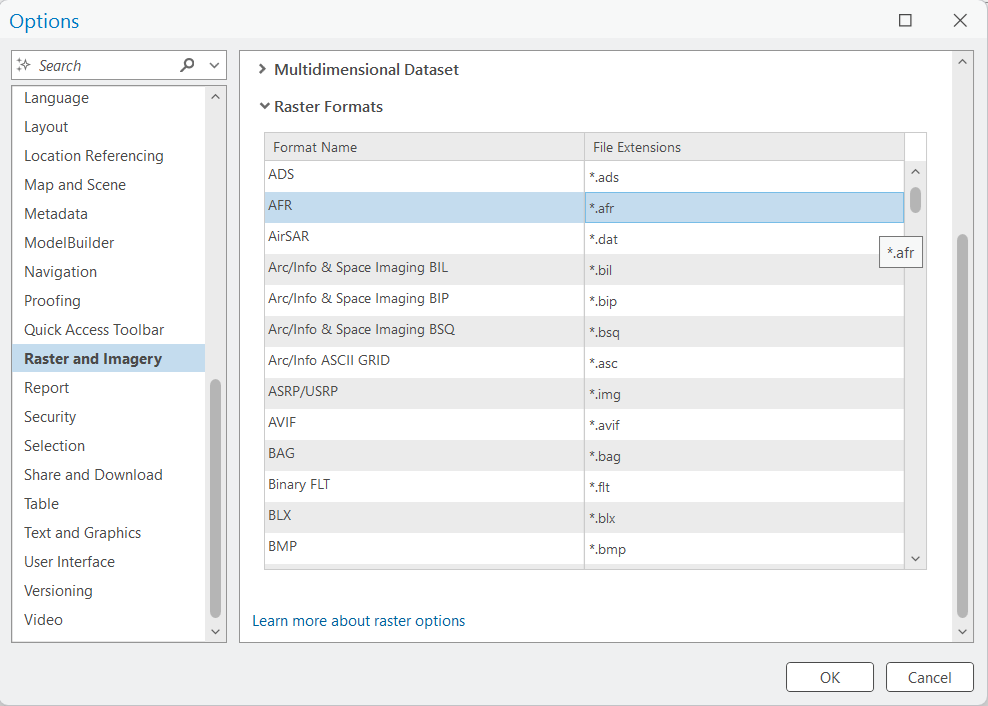
\includegraphics[width=0.75\textwidth,height=\textheight]{images/conversion_formatos/raster_formats_arcgis.png}

}

\caption{\label{fig-raster-arcgis}Formatos ráster soportados en el menú
de opciones de ArcGIS Pro.}

\end{figure}%

Ver la
\href{https://pro.arcgis.com/en/pro-app/latest/help/data/imagery/supported-raster-dataset-file-formats.htm}{ayuda}
para mayor información.

\subsubsection{QGIS}

Menú \texttt{Settings} (Configuración) -\textgreater{} \texttt{Options}
(Opciones) -\textgreater{} \texttt{GDAL} -\textgreater{} pestaña
\texttt{Raster\ Drivers} (Controladores ráster)

\begin{figure}

\centering{

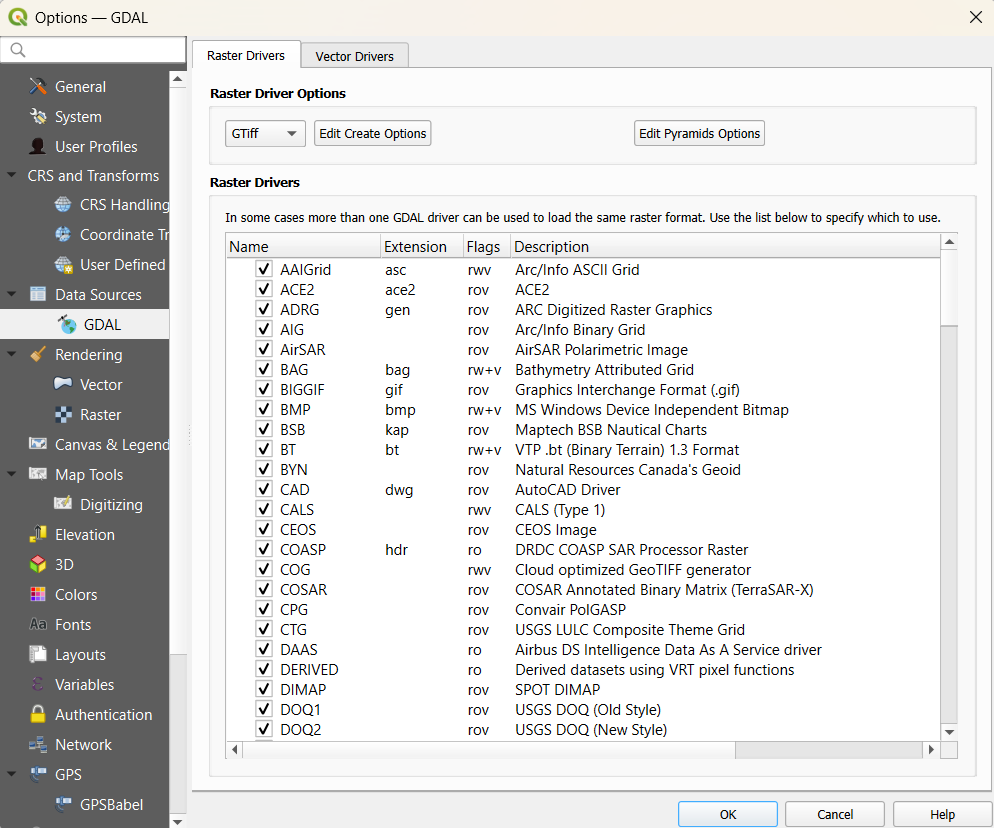
\includegraphics[width=0.75\textwidth,height=\textheight]{images/conversion_formatos/formatos_raster_qgis_gdal.png}

}

\caption{\label{fig-raster-qgis}Formatos ráster y capacidades GDAL
listados en QGIS.}

\end{figure}%

\textbf{Explicación de los \emph{Flags} (Capacidades) en QGIS:}

La columna \textbf{Flags} en la tabla de GDAL indica los permisos
exactos que tiene QGIS para interactuar con cada formato de archivo.
Cada letra representa una capacidad específica:

\begin{itemize}
\tightlist
\item
  \textbf{\texttt{r} (Read - Lectura):} QGIS puede abrir y visualizar el
  archivo.
\item
  \textbf{\texttt{w} (Write - Escritura):} QGIS puede crear, guardar o
  exportar un archivo nuevo en este formato desde cero.
\item
  \textbf{\texttt{+} (Update - Actualización):} QGIS puede modificar un
  archivo existente (por ejemplo, editar sus metadatos o cambiar valores
  de píxeles) sin tener que crear un archivo completamente nuevo.
\item
  \textbf{\texttt{v} (Virtual IO - Entrada/Salida Virtual):} QGIS puede
  leer o escribir este archivo dentro de ``sistemas de archivos
  virtuales''. Esto permite abrir un ráster que está comprimido dentro
  de un \texttt{.zip} o alojado en la web mediante una URL, sin
  necesidad de extraerlo o descargarlo previamente.
\end{itemize}

\textbf{Ejemplos de combinaciones comunes:}

\begin{itemize}
\tightlist
\item
  \textbf{\texttt{ro}:} Solo lectura. Se puede visualizar, pero no
  modificar ni crear, y no soporta archivos virtuales.
\item
  \textbf{\texttt{rov}:} Solo lectura + soporte virtual. Se puede
  visualizar directamente desde un \texttt{.zip} o desde internet.
\item
  \textbf{\texttt{rwv}:} Lectura, escritura + soporte virtual. Se puede
  abrir, crear nuevos archivos y usar archivos virtuales.
\item
  \textbf{\texttt{rw+v}:} Control total. Permite abrir, crear,
  actualizar un archivo existente y soporta lectura desde archivos
  comprimidos o la web.
\end{itemize}

\subsection{Tipos de formatos vector
soportados}\label{tipos-de-formatos-vector-soportados}

\subsubsection{ArcGIS}

A diferencia de los formatos ráster, \textbf{ArcGIS Pro no centraliza el
listado de formatos vectoriales en su menú de opciones}. El soporte
nativo para vectores está integrado en el núcleo del software
(Geodatabases de archivos y móviles, Shapefiles, KML, archivos CAD,
etc.).

Para visualizar los tipos de archivos vectoriales y bases de datos
espaciales que el software reconoce directamente, la forma más sencilla
es a través del cuadro de diálogo al agregar datos:

Pestaña \texttt{Map} (Mapa) -\textgreater{} \texttt{Add\ Data} (Agregar
datos) -\textgreater{} \texttt{Browse...} (Examinar\ldots). En la
ventana ``Add data'', al desplegar la lista de tipos (Tipo de elemento)
al lado de \textbf{Name} , verás los formatos soportados.

\begin{figure}

\centering{

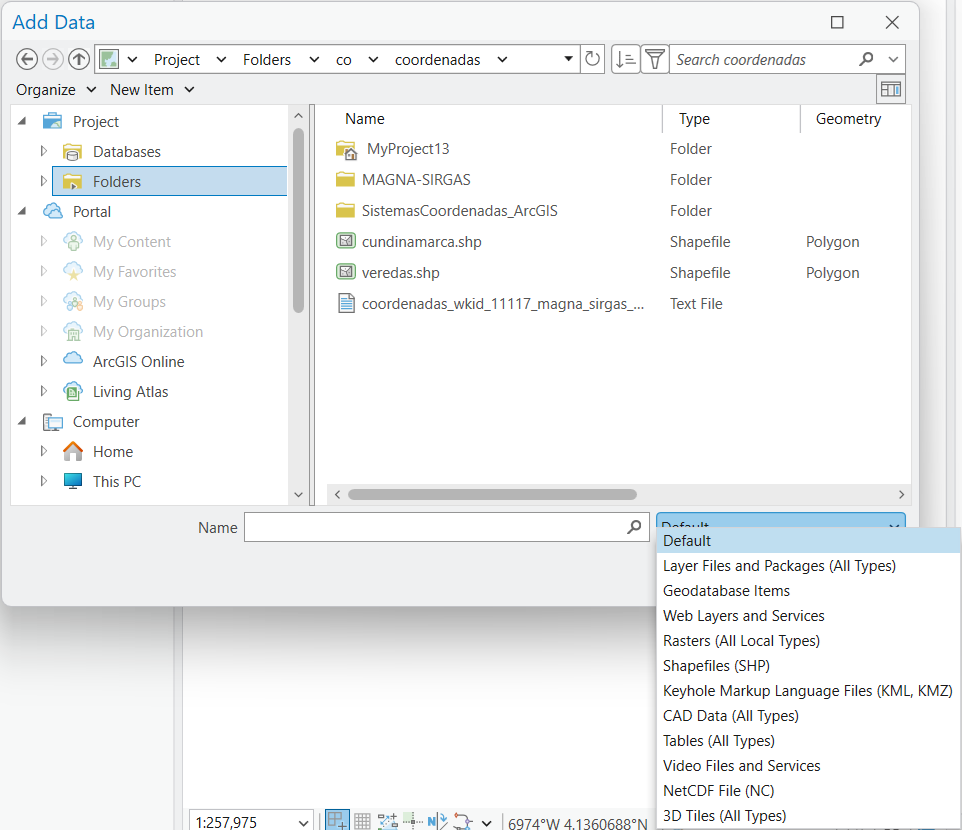
\includegraphics[width=0.75\textwidth,height=\textheight]{images/conversion_formatos/vector_formats_arcgis.png}

}

\caption{\label{fig-vector-arcgis}Formatos vectoriales reconocidos en el
cuadro de diálogo Add Data de ArcGIS Pro.}

\end{figure}%

\begin{quote}
\textbf{Nota:} Para leer y escribir en formatos vectoriales no nativos o
más especializados, ArcGIS Pro utiliza una extensión llamada
\textbf{Data Interoperability}, la cual habilita el soporte para más de
300 formatos adicionales. Puedes consultar la lista completa en la
\href{https://pro.arcgis.com/en/pro-app/latest/help/projects/supported-data-types-and-items.htm}{ayuda
oficial de Esri}.
\end{quote}

\subsubsection{QGIS}

QGIS utiliza la biblioteca \textbf{OGR} (parte del proyecto GDAL) para
la lectura y escritura de datos vectoriales. Puedes ver la lista
completa de formatos, sus controladores (drivers) y capacidades en:

Menú \texttt{Settings} (Configuración) -\textgreater{} \texttt{Options}
(Opciones) -\textgreater{} \texttt{GDAL} -\textgreater{} pestaña
\texttt{Vector\ Drivers} (Controladores vectoriales).

\begin{figure}

\centering{

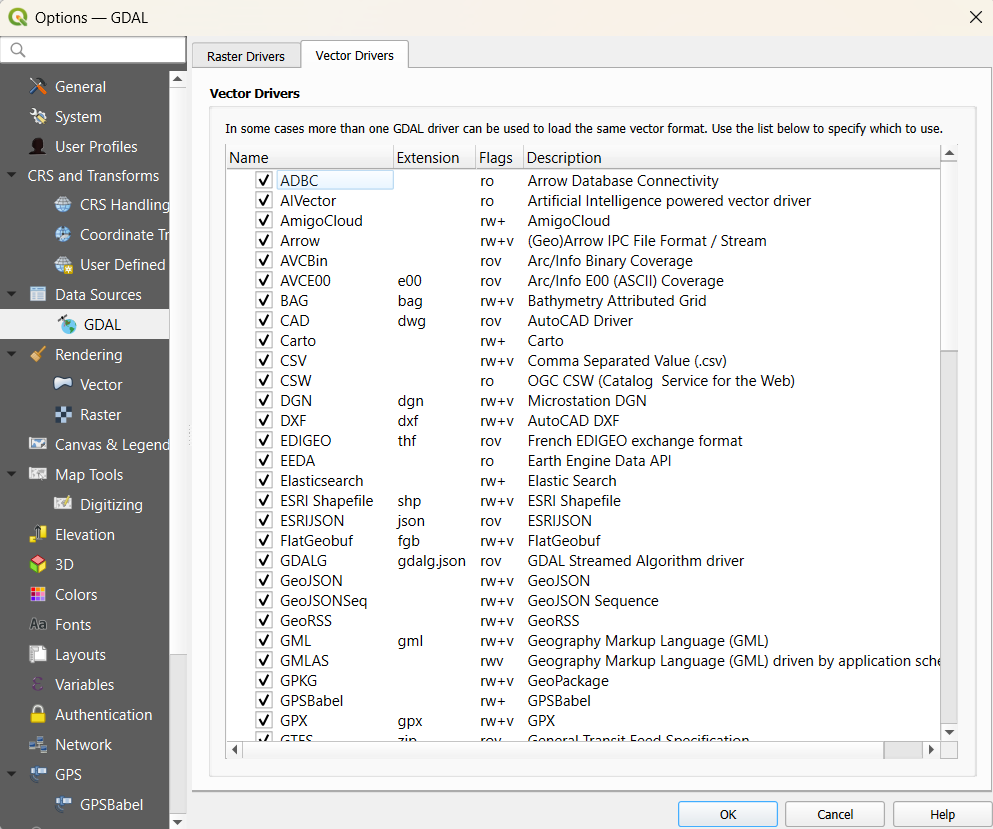
\includegraphics[width=0.75\textwidth,height=\textheight]{images/conversion_formatos/formatos_vector_qgis_ogr.png}

}

\caption{\label{fig-vector-qgis}Lista de controladores OGR y sus
capacidades en QGIS.}

\end{figure}%

\textbf{Capacidades de los Drivers OGR (Banderas / Flags):}

Al igual que en los ráster, los controladores vectoriales muestran
banderas (\textbf{Flags}) en QGIS que indican exactamente qué permisos
tiene el software para interactuar con cada formato. Estas letras se
traducen en las siguientes capacidades:

\begin{itemize}
\tightlist
\item
  \textbf{\texttt{r} (Read - Lectura / ReadOnly):} El formato puede ser
  visualizado. Si el controlador solo muestra la bandera \texttt{ro},
  significa que es de \textbf{Solo Lectura} y no puede ser editado (ej.
  algunos formatos web o de OpenStreetMap).
\item
  \textbf{\texttt{w} (Write - Escritura / Read/Write):} Indica que QGIS
  puede crear y exportar archivos nuevos en este formato. Al combinarse
  con lectura (\texttt{rw}), permite la creación y edición completa de
  entidades y atributos (ej. \textbf{GeoPackage}, \textbf{Shapefile}).
\item
  \textbf{\texttt{+} (Update - Actualización):} Significa que el
  controlador puede modificar o actualizar un archivo existente sin
  tener que sobrescribirlo por completo.
\item
  \textbf{\texttt{v} (Virtual IO - Entrada/Salida Virtual):} Permite que
  QGIS lea archivos directamente desde ``sistemas virtuales'', como
  servicios web, la nube o dentro de archivos comprimidos
  (\textbf{.zip}, \textbf{.tar}) sin necesidad de extraerlos previamente
  en el disco duro.
\end{itemize}

\section{Opciones de conversión de formatos (ArcGIS Pro -
QGIS)}\label{opciones-de-conversiuxf3n-de-formatos-arcgis-pro---qgis}

\subsection{ArcGIS Pro}

En ArcGIS Pro existen principalmente tres métodos para la conversión e
intercambio de formatos de datos espaciales. A continuación, se detalla
cada uno de ellos:

\subsubsection{1. Desde las herramientas de geoprocesamiento
(toolbox)}\label{desde-las-herramientas-de-geoprocesamiento-toolbox}

Esta es la forma más estructurada y completa, ideal para ejecutar
procesos masivos (Batch) o aplicar herramientas de conversión muy
específicas.

\begin{itemize}
\tightlist
\item
  \textbf{Ruta:} Menú \texttt{View} (Vista) -\textgreater{} botón
  \texttt{Geoprocessing} (Geoprocesamiento) -\textgreater{} pestaña
  \texttt{Toolboxes} (Cajas de herramientas) -\textgreater{} expandir
  \texttt{Conversion\ Tools} (Herramientas de conversión).
\end{itemize}

\begin{figure}

\centering{

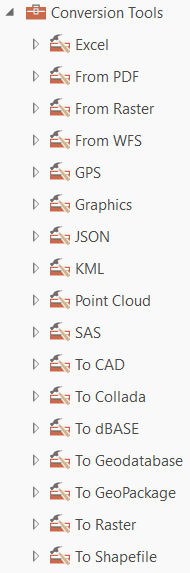
\includegraphics[width=0.25\textwidth,height=\textheight]{images/conversion_formatos/conversion_tools_arcgis_pro.png}

}

\caption{\label{fig-conv-tools-arcgis}Herramientas de conversión en la
caja de procesos de ArcGIS Pro.}

\end{figure}%

Dentro de la caja de \textbf{Conversion Tools} (Herramientas de
conversión), las opciones se agrupan según el formato de origen o
destino:

\begin{itemize}
\item
  \textbf{Conversiones Ráster:}

  \begin{itemize}
  \item
    \textbf{From Raster} (Desde ráster): Convierte datos ráster a otros
    formatos (principalmente vectoriales, como polígonos, líneas o
    puntos).

    \begin{figure}

    \centering{

    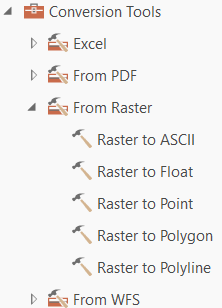
\includegraphics[width=0.3\textwidth,height=\textheight]{images/conversion_formatos/conversion_tools_from_raster_pro.png}

    }

    \caption{\label{fig-from-raster-arcgis}Opciones para convertir desde
    un formato ráster.}

    \end{figure}%
  \item
    \textbf{To Raster} (A ráster): Convierte otros formatos (como
    entidades vectoriales) a formato ráster.

    \begin{figure}

    \centering{

    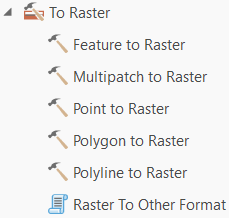
\includegraphics[width=0.3\textwidth,height=\textheight]{images/conversion_formatos/conversion_tools_to_raster_pro.png}

    }

    \caption{\label{fig-to-raster-arcgis}Opciones para convertir hacia
    un formato ráster.}

    \end{figure}%
  \item
    \textbf{To GeoPackage} (A GeoPackage): Permite agregar un ráster
    existente a un archivo GeoPackage mediante
    \texttt{Add\ Raster\ to\ GeoPackage} (Agregar ráster a GeoPackage).
  \end{itemize}
\item
  \textbf{Conversiones Vectoriales y Web:}

  \begin{itemize}
  \tightlist
  \item
    \textbf{To Geodatabase} (A geodatabase): Múltiples opciones para
    migrar formatos vectoriales (e incluso datos ráster usando
    \texttt{Raster\ to\ Geodatabase} {[}Ráster a geodatabase{]}) hacia
    una File o Enterprise Geodatabase.
  \item
    \textbf{To Shapefile} (A shapefile): Convierte entidades vectoriales
    almacenadas en Geodatabases (Feature Classes) al formato tradicional
    Shapefile.
  \item
    \textbf{To CAD} (A CAD): Exporta datos vectoriales a formatos de
    diseño asistido por computadora (ej. DWG, DXF).
  \item
    \textbf{From WFS} (Desde WFS): Convierte un servicio Web Feature
    Service a diferentes formatos vectoriales locales. Consulta la
    \href{https://pro.arcgis.com/en/pro-app/latest/tool-reference/conversion/wfs-to-feature-class.htm}{ayuda
    en línea aquí}.
  \end{itemize}
\item
  \textbf{Conversiones Bidireccionales (Desde y Hacia):}

  \begin{itemize}
  \tightlist
  \item
    \textbf{GPS:} Convierte archivos GPX a vectores usando
    \texttt{GPX\ to\ features} (GPX a entidades) o viceversa con
    \texttt{Features\ to\ GPX} (Entidades a GPX).
  \item
    \textbf{JSON:} Transforma archivos GeoJSON a entidades vectoriales y
    de vuelta.
  \item
    \textbf{KML:} Permite convertir archivos, capas o mapas enteros a
    formato KML/KMZ o viceversa.
  \end{itemize}
\end{itemize}

\begin{center}\rule{0.5\linewidth}{0.5pt}\end{center}

\subsubsection{2. Desde la capa en el mapa (contents
pane)}\label{desde-la-capa-en-el-mapa-contents-pane}

Este método es el más rápido y práctico cuando ya tienes los datos
cargados en tu vista de mapa y necesitas exportar la capa activa. Es
especialmente útil porque respeta las selecciones (si tienes polígonos
seleccionados, solo exportará esos). Con esta opción se habilitan las
opciones de transformación de datos con las coordenadas del mapa (usando
la reproyección al vuelo aplicada a la capa) o de la capa.

\begin{itemize}
\tightlist
\item
  \textbf{Ruta:} \texttt{Clic\ Derecho} sobre la capa (en el panel
  \texttt{Contents} {[}Contenido{]}) -\textgreater{} \texttt{Data}
  (Datos) -\textgreater{} \texttt{Export\ Features} (Exportar entidades)
  (para vectores) o \texttt{Export\ Raster} (Exportar ráster) (para
  imágenes).
\end{itemize}

\begin{figure}

\centering{

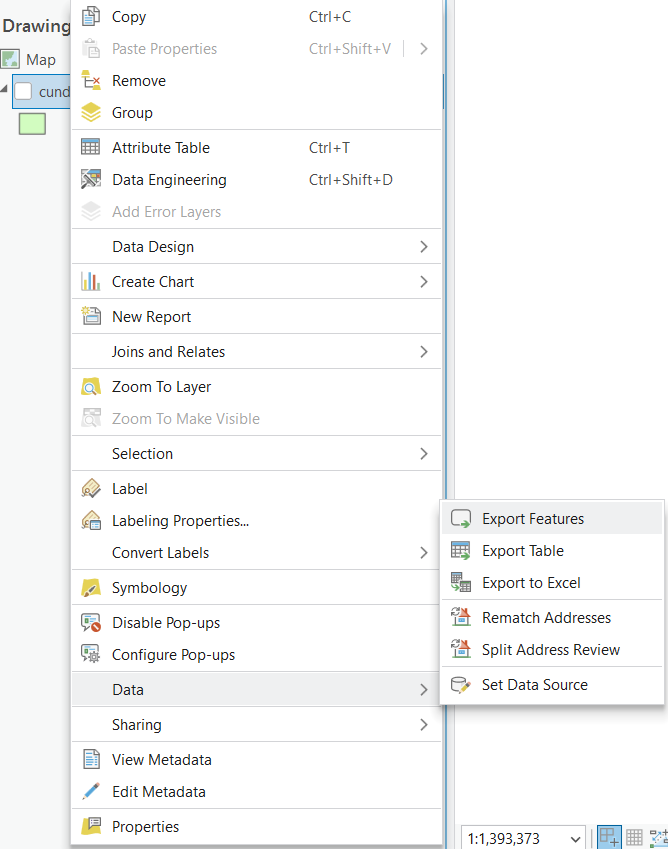
\includegraphics[width=0.75\textwidth,height=\textheight]{images/conversion_formatos/conversion_formatos_desde_mapa_pro.png}

}

\caption{\label{fig-export-map-arcgis}Exportación directa de entidades
desde el panel de contenido en ArcGIS Pro.}

\end{figure}%

\begin{center}\rule{0.5\linewidth}{0.5pt}\end{center}

\subsubsection{3. Desde el panel de catálogo (catalog
pane)}\label{desde-el-panel-de-catuxe1logo-catalog-pane}

Ideal para gestionar y convertir archivos directamente desde el disco
duro o bases de datos sin necesidad de cargarlos previamente al mapa
para visualizarlos.

\begin{itemize}
\tightlist
\item
  \textbf{Ruta:} Para abrir el catálogo ve al menú \texttt{View} (Vista)
  -\textgreater{} \texttt{Catalog\ Pane} (Panel de catálogo).
\item
  \textbf{Proceso:} \texttt{Clic\ Derecho} sobre el dato de interés
  -\textgreater{} \texttt{Export} (Exportar) -\textgreater{}
  \emph{Seleccionar la opción deseada}.
\end{itemize}

\begin{quote}
\textbf{Nota:} Las opciones de exportación que aparecen en el menú
desplegable son dinámicas y dependen estrictamente del tipo de archivo
seleccionado por el usuario. La imagen a continuación muestra el ejemplo
de las opciones habilitadas al seleccionar un archivo
\textbf{Shapefile}:
\end{quote}

\begin{figure}

\centering{

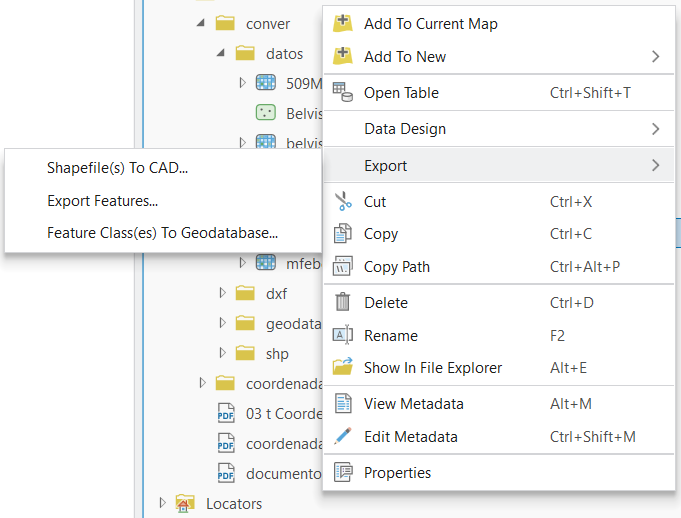
\includegraphics[width=0.75\textwidth,height=\textheight]{images/conversion_formatos/intercambio_de_formatos_desde_el_catalogo_pro.png}

}

\caption{\label{fig-export-catalog-arcgis}Opciones de exportación
contextuales desde el panel de catálogo en ArcGIS Pro.}

\end{figure}%

\subsection{QGIS}

De manera análoga a ArcGIS Pro, QGIS ofrece diferentes vías para la
conversión e intercambio de formatos, apoyándose fuertemente en las
librerías GDAL (para ráster) y OGR (para vectores). A continuación, se
detallan los tres métodos principales:

\subsubsection{1. Desde la caja de herramientas de procesos (processing
toolbox)}\label{desde-la-caja-de-herramientas-de-procesos-processing-toolbox}

Este método es ideal para procesos por lotes (Batch) y para acceder a
los algoritmos nativos de GDAL/OGR con control total sobre los
parámetros de conversión.

\begin{itemize}
\tightlist
\item
  \textbf{Ruta:} Menú \texttt{Processing} (Procesos) -\textgreater{}
  \texttt{Toolbox} (Caja de herramientas).
\end{itemize}

\begin{figure}

\centering{

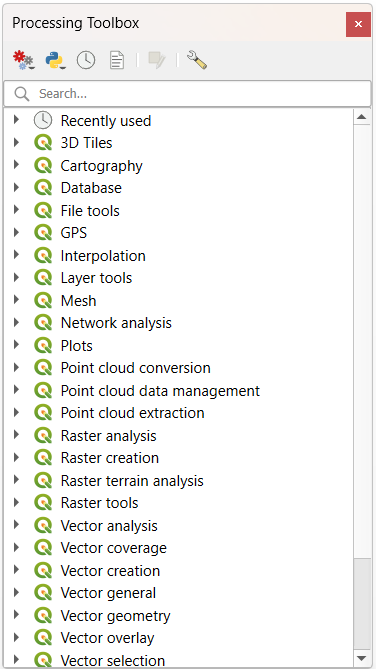
\includegraphics[width=0.4\textwidth,height=\textheight]{images/conversion_formatos/caja_herramientas_qgis.png}

}

\caption{\label{fig-toolbox-qgis}Caja de herramientas de procesos en
QGIS.}

\end{figure}%

Dentro de la caja de herramientas, las opciones de conversión se
encuentran distribuidas en diferentes grupos, principalmente bajo
\textbf{GDAL}, \textbf{Database} (Base de datos) y \textbf{Vector
general} (Vectorial general):

\begin{itemize}
\item
  \textbf{Conversiones Ráster y Vectoriales (GDAL):}

  \begin{itemize}
  \tightlist
  \item
    \textbf{En \texttt{GDAL} -\textgreater{} \texttt{Raster\ conversion}
    (Conversión ráster):}

    \begin{itemize}
    \tightlist
    \item
      \texttt{Translate\ (convert\ format)} (Traducir {[}convertir
      formato{]}): Es la herramienta principal para convertir entre
      formatos ráster (ej. TIFF a JPEG, o a un GeoPackage).
    \item
      \texttt{Polygonize\ (raster\ to\ vector)} (Poligonizar {[}ráster a
      vector{]}): Convierte píxeles de un ráster a polígonos
      vectoriales.
    \end{itemize}

    \begin{figure}

    \centering{

    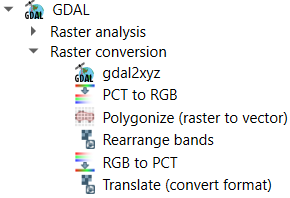
\includegraphics[width=0.4\textwidth,height=\textheight]{images/conversion_formatos/conversion_raster_gdal_qgis.png}

    }

    \caption{\label{fig-gdal-raster-qgis}Herramientas de conversión
    ráster de GDAL en QGIS.}

    \end{figure}%
  \item
    \textbf{En \texttt{GDAL} -\textgreater{} \texttt{Vector\ conversion}
    (Conversión vectorial):}

    \begin{itemize}
    \tightlist
    \item
      \texttt{Convert\ format} (Convertir formato): Permite convertir
      masivamente formatos vectoriales (ej. de Shapefile a GeoPackage,
      GeoJSON, KML, etc.).
    \item
      \texttt{Rasterize\ (vector\ to\ raster)} (Rasterizar {[}vector a
      ráster{]}): Convierte entidades vectoriales a formato ráster.
    \end{itemize}

    \begin{figure}

    \centering{

    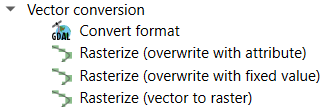
\includegraphics[width=0.4\textwidth,height=\textheight]{images/conversion_formatos/rasteriza_vector_to_raster.png}

    }

    \caption{\label{fig-gdal-vector-qgis}Herramientas de conversión
    vectorial de GDAL en QGIS.}

    \end{figure}%
  \end{itemize}
\item
  \textbf{Conversiones a Bases de Datos y Otros Formatos (Export):}

  \begin{itemize}
  \tightlist
  \item
    \textbf{En el grupo \texttt{Database} (Base de datos):} Encuentras
    algoritmos específicos para bases de datos espaciales, como
    \texttt{Export\ to\ PostgreSQL} (Exportar a PostgreSQL) y
    \texttt{Export\ to\ SpatiaLite} (Exportar a SpatiaLite).
  \item
    \textbf{En el grupo \texttt{Vector\ general} (Vectorial general):}
    Herramientas nativas de QGIS como
    \texttt{Save\ vector\ features\ to\ file} (Guardar entidades
    vectoriales a archivo) (que funciona como un guardado masivo) y
    \texttt{Export\ layers\ to\ DXF} (Exportar capas a DXF) para
    transformar datos espaciales en formatos CAD.
  \item
    \textbf{En \texttt{GDAL} -\textgreater{}
    \texttt{Vector\ miscellaneous} (Miscelánea vectorial):} Opciones
    alternativas manejadas por GDAL para conectarse y exportar datos a
    bases de datos como PostgreSQL.
  \end{itemize}
\end{itemize}

\begin{center}\rule{0.5\linewidth}{0.5pt}\end{center}

\subsubsection{2. Desde la capa en el panel de capas (layers
panel)}\label{desde-la-capa-en-el-panel-de-capas-layers-panel}

Al igual que en ArcGIS Pro, este es el método más utilizado en el
trabajo diario cuando la capa ya está cargada en el lienzo del mapa.
Permite guardar selecciones específicas y ofrece un control granular
sobre qué atributos exportar. También permite aplicar una transformación
de coordenadas al vuelo (reproyectar) durante la exportación.

\begin{itemize}
\tightlist
\item
  \textbf{Ruta:} \texttt{Clic\ Derecho} sobre la capa (en el panel
  \texttt{Layers} (Capas)) -\textgreater{} \texttt{Export} (Exportar)
  -\textgreater{} \texttt{Save\ Features\ As...} (Guardar entidades
  como\ldots) (para vectores) o \texttt{Save\ As...} (Guardar
  como\ldots) (para imágenes).
\end{itemize}

\begin{figure}

\centering{

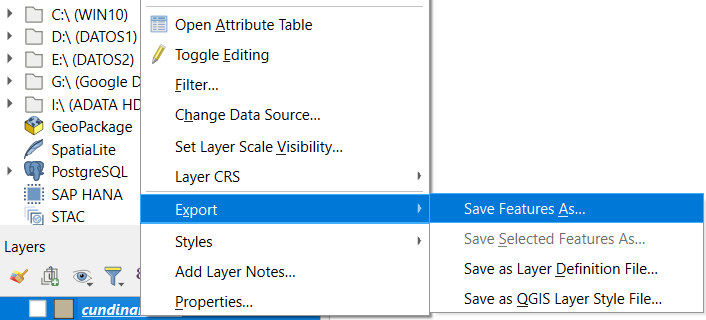
\includegraphics[width=0.65\textwidth,height=\textheight]{images/conversion_formatos/exportar_capa_qgis.png}

}

\caption{\label{fig-export-layer-qgis}Exportación de datos espaciales
desde el panel de capas en QGIS.}

\end{figure}%

\begin{quote}
\textbf{Nota:} El cuadro de diálogo de
\texttt{Save\ Vector\ Layer\ as...} (Guardar capa vectorial como\ldots)
es extremadamente potente. No solo permite cambiar el formato, sino que
también te permite cambiar el Sistema de Referencia de Coordenadas
(CRS), seleccionar qué campos de la tabla de atributos conservar y
definir parámetros específicos de la capa (Layer Options) como la
geometría.
\end{quote}

\begin{figure}

\centering{

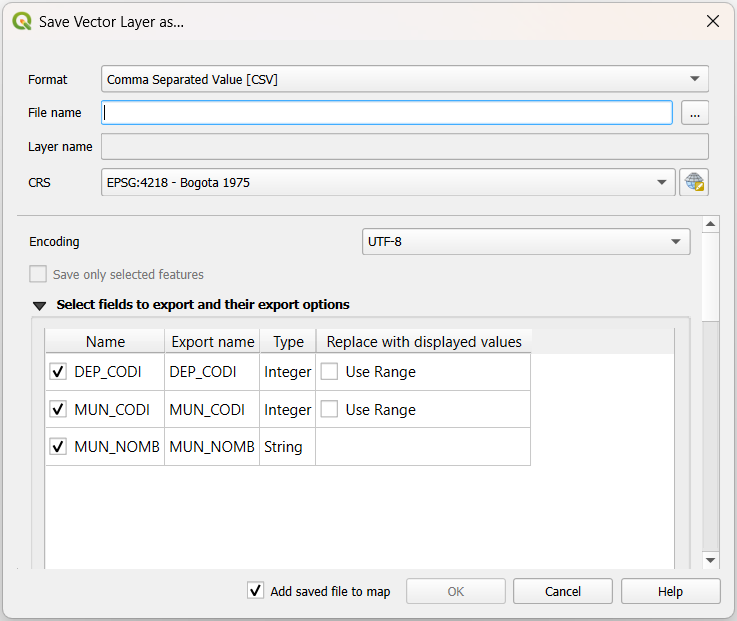
\includegraphics[width=0.75\textwidth,height=\textheight]{images/conversion_formatos/save_features_as_dialog_qgis.png}

}

\caption{\label{fig-save-vector-qgis}Cuadro de diálogo de guardado
avanzado vectorial en QGIS.}

\end{figure}%

\begin{center}\rule{0.5\linewidth}{0.5pt}\end{center}

\subsubsection{3. Desde el panel del navegador (browser
panel)}\label{desde-el-panel-del-navegador-browser-panel}

El panel del navegador en QGIS actúa como un catálogo. Aunque
tradicionalmente se usa más para cargar datos arrastrándolos al mapa,
también permite exportar datos físicos de manera directa, así como
gestionar bases de datos espaciales.

\begin{itemize}
\tightlist
\item
  \textbf{Ruta:} Para abrir el navegador ve al menú \texttt{View} (Ver)
  -\textgreater{} \texttt{Panels} (Paneles) -\textgreater{}
  \texttt{Browser} (Navegador).
\end{itemize}

\begin{figure}

\centering{

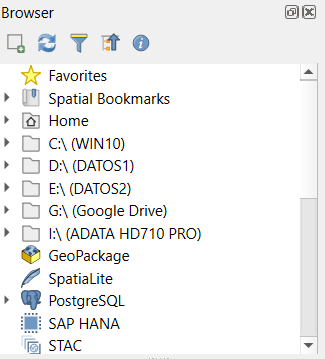
\includegraphics[width=0.35\textwidth,height=\textheight]{images/conversion_formatos/panel_navegador_qgis.png}

}

\caption{\label{fig-browser-qgis}Panel del navegador utilizado para
gestionar archivos en QGIS.}

\end{figure}%

\begin{itemize}
\tightlist
\item
  \textbf{Proceso:} \texttt{Clic\ Derecho} sobre el archivo o tabla de
  base de datos de interés -\textgreater{} \texttt{Export\ Layer}
  (Exportar capa) -\textgreater{} \texttt{To\ File...} (A
  archivo\ldots). Aparecerá nuevamente el cuadro de diálogo
  \texttt{Save\ Vector\ Layer\ as...} (Guardar capa vectorial
  como\ldots).
\end{itemize}

\begin{figure}

\centering{

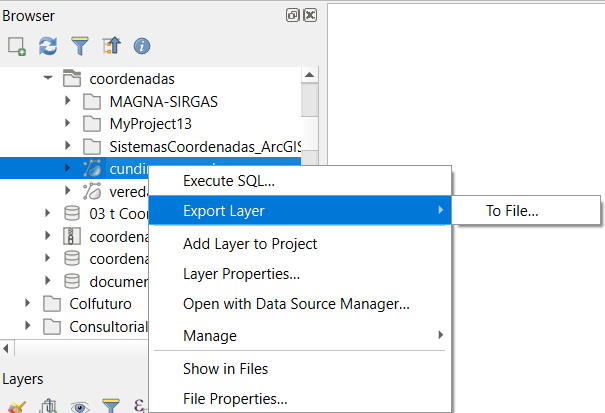
\includegraphics[width=0.65\textwidth,height=\textheight]{images/conversion_formatos/exportar_navegador_qgis.png}

}

\caption{\label{fig-export-browser-qgis}Proceso de exportación directa
desde el navegador de QGIS.}

\end{figure}%

\begin{quote}
\textbf{Tip para bases de datos:} Desde el navegador, una de las formas
más rápidas de convertir formatos es simplemente arrastrar un archivo
(como un Shapefile) y soltarlo dentro de una conexión de base de datos
(como un GeoPackage o PostGIS) para importarlo instantáneamente.
\end{quote}

\subsection{GRASS}

GRASS GIS es un software espacial de grado científico que viene
integrado como un proveedor nativo dentro de la caja de herramientas de
procesos de QGIS. Sus herramientas de conversión son vitales en análisis
avanzados porque exigen y aplican una limpieza topológica estricta a los
datos geométricos.

GRASS GIS funciona bajo una estructura particular organizada en
\textbf{Database}, \textbf{Location} y \textbf{Mapset}, la cual
garantiza la \emph{integridad topológica} al no operar directamente
sobre archivos sueltos. Todos los algoritmos de GRASS siguen una
nomenclatura lógica: \texttt{módulo.acción.formato}. El módulo vectorial
usa la letra \texttt{v} y el módulo ráster usa la letra \texttt{r}. Las
acciones son \texttt{in} para importar datos a la estructura particular
de GRASS y \texttt{out} para exportar datos desde esta hacia otras
plataformas.

\begin{figure}

\centering{

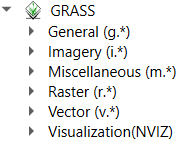
\includegraphics[width=0.25\textwidth,height=\textheight]{images/conversion_formatos/herramientas_grass_qgis.png}

}

\caption{\label{fig-grass-tools}Estructura de los módulos de GRASS en la
caja de procesos de QGIS.}

\end{figure}%

\subsubsection{1. Módulos de importación
(in)}\label{muxf3dulos-de-importaciuxf3n-in}

Sirven para ``convertir'' e ingresar datos externos hacia el estricto
formato interno de GRASS. Las herramientas de importación terminan en
\texttt{.in} (del inglés \emph{input} {[}entrada{]}).

\begin{itemize}
\tightlist
\item
  \textbf{Vectoriales (\texttt{v.in.*}):} ~ ~ * Encontrarás comandos muy
  útiles para importar y corregir topología de varios formatos. Ejemplos
  destacados incluyen \texttt{v.in.wfs} para traer datos de servicios
  web, o \texttt{v.in.e00} para leer archivos antiguos de intercambio.
\end{itemize}

\begin{figure}

\centering{

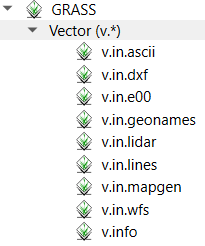
\includegraphics[width=0.3\textwidth,height=\textheight]{images/conversion_formatos/grass_import_vector_qgis.png}

}

\caption{\label{fig-grass-import-vector}Herramientas de importación
vectorial en GRASS.}

\end{figure}%

\begin{itemize}
\tightlist
\item
  \textbf{Ráster (\texttt{r.in.*}):} ~ ~ * Existen importadores
  dedicados como \texttt{r.in.lidar} para datos de elevación de nubes de
  puntos.
\end{itemize}

\begin{figure}

\centering{

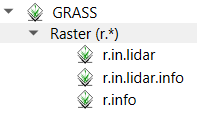
\includegraphics[width=0.3\textwidth,height=\textheight]{images/conversion_formatos/grass_import_raster_qgis.png}

}

\caption{\label{fig-grass-import-raster}Herramientas de importación
ráster en GRASS.}

\end{figure}%

\subsubsection{2. Módulos de exportación
(out)}\label{muxf3dulos-de-exportaciuxf3n-out}

Se utilizan para ``convertir'' y sacar los datos ya procesados en el
entorno topológico de GRASS hacia formatos estándar reconocibles por
otros SIG. Estas herramientas terminan en \texttt{.out} (del inglés
\emph{output} {[}salida{]}).

\begin{itemize}
\tightlist
\item
  \textbf{Vectoriales (\texttt{v.out.*}):} ~ ~ * Herramientas como
  \texttt{v.out.dxf} para enviar geometrías a CAD, o
  \texttt{v.out.postgis} que facilita la carga directa y estructurada a
  una base de datos espacial PostgreSQL.
\end{itemize}

\begin{figure}

\centering{

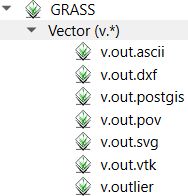
\includegraphics[width=0.3\textwidth,height=\textheight]{images/conversion_formatos/grass_export_vector_qgis.png}

}

\caption{\label{fig-grass-export-vector}Herramientas de exportación
vectorial en GRASS.}

\end{figure}%

\begin{itemize}
\tightlist
\item
  \textbf{Ráster (\texttt{r.out.*}):} ~ ~ * GRASS ofrece un nivel de
  detalle avanzado para exportar matrices numéricas. Puedes convertir
  tus modelos ráster a formatos de texto plano legibles por máquina con
  \texttt{r.out.ascii}, exportarlos como imágenes ligeras para la web
  con \texttt{r.out.png}, o utilizar formatos matemáticos como
  \texttt{r.out.mat}.
\end{itemize}

\begin{figure}

\centering{

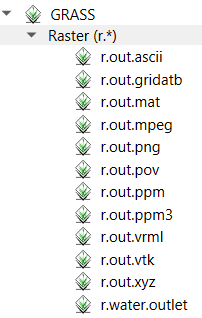
\includegraphics[width=0.3\textwidth,height=\textheight]{images/conversion_formatos/grass_export_raster_qgis.png}

}

\caption{\label{fig-grass-export-raster}Herramientas de exportación
ráster en GRASS.}

\end{figure}%

\section{Ejercicios}\label{ejercicios}

\subsection{Ejercicio 1: Migración de bases de datos obsoletas (.mdb) a
formatos
modernos}\label{ejercicio-1-migraciuxf3n-de-bases-de-datos-obsoletas-.mdb-a-formatos-modernos}

\textbf{Nota importante:} Las bases de datos personales de Esri
(\texttt{.mdb}) están construidas sobre tecnología antigua de 32 bits de
Microsoft Access. Dado que ArcGIS Pro es una arquitectura moderna de 64
bits, ha dejado de soportar este formato. Para recuperar, leer y
modernizar estos datos, utilizaremos QGIS como ``puente'' gracias a su
potente compatibilidad mediante la librería GDAL/OGR.

A continuación, se presentan tres métodos en QGIS para migrar todos los
datos de una \texttt{.mdb} hacia formatos modernos como GeoPackage
(\texttt{.gpkg}) o File Geodatabase (\texttt{.gdb}).

\subsubsection{Método A: Empaquetar capas a
GeoPackage}\label{muxe9todo-a-empaquetar-capas-a-geopackage}

\begin{itemize}
\tightlist
\item
  \textbf{Objetivo:} Agrupar todas las capas cargadas desde la base de
  datos antigua en un solo archivo estándar y abierto (GeoPackage).
\item
  \textbf{Herramientas:} Menú \texttt{Processing} (Procesos)
  -\textgreater{} \texttt{Toolbox} (Caja de herramientas)
  -\textgreater{} \texttt{Database} (Base de datos) -\textgreater{}
  \texttt{Package\ layers} (Empaquetar capas).
\item
  \textbf{Proceso:} Cargue primero las capas del \texttt{.mdb} al panel
  de capas de QGIS. Abra la herramienta, seleccione las 7 capas cargadas
  como entrada (también puede arrastrar todas las capas desde el panel
  de capas hacia la herramienta) y ejecute.
\item
  \textbf{Datos de entrada:} Capas cargadas desde
  \texttt{GreenvalleyDB.mdb}.
\item
  \textbf{Datos de salida:} \texttt{GreenValleyDB.gpkg} (almacenado en
  la carpeta \texttt{geodatabase}).
\end{itemize}

\begin{figure}

\centering{

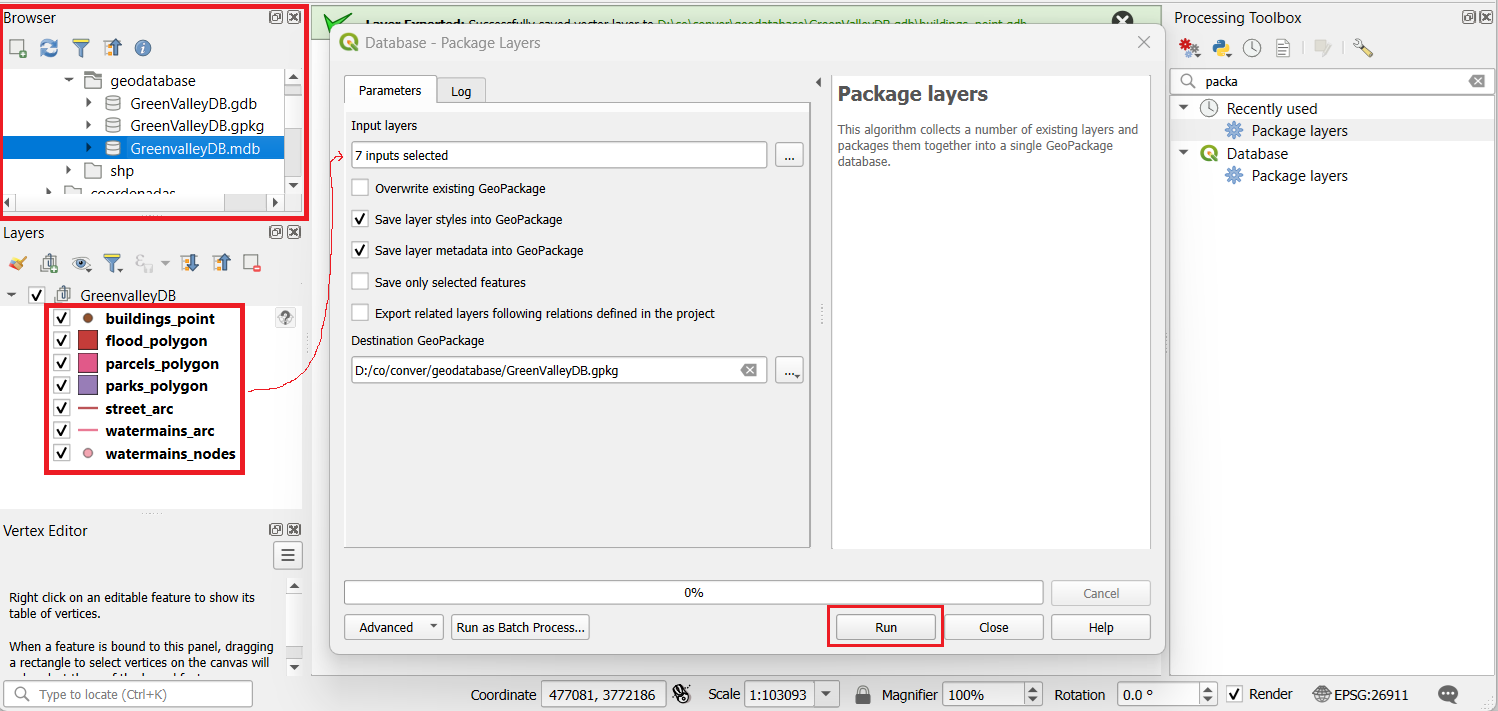
\includegraphics[width=1\textwidth,height=\textheight]{images/conversion_formatos/package_layer_qgis_mdb_gdb.png}

}

\caption{\label{fig-package-layers}Herramienta para empaquetar múltiples
capas a un GeoPackage en QGIS.}

\end{figure}%

\subsubsection{Método B: Conversión directa a File Geodatabase
(GDAL)}\label{muxe9todo-b-conversiuxf3n-directa-a-file-geodatabase-gdal}

\begin{itemize}
\tightlist
\item
  \textbf{Objetivo:} Convertir la base de datos antigua completa
  directamente a una File Geodatabase de Esri (\texttt{.gdb}) en un solo
  paso mediante procesos por lotes de GDAL.
\item
  \textbf{Herramientas:} Menú \texttt{Processing} (Procesos)
  -\textgreater{} \texttt{Toolbox} (Caja de herramientas)
  -\textgreater{} \texttt{GDAL} -\textgreater{}
  \texttt{Vector\ conversion} (Conversión vectorial) -\textgreater{}
  \texttt{Convert\ format} (Convertir formato).
\item
  \textbf{Proceso:} Ingrese la ruta del archivo \texttt{.mdb} original.
  Es vital marcar la casilla \textbf{``Convert all layers from
  dataset''} (Convertir todas las capas del conjunto de datos) para que
  migre toda la base de datos y no solo una tabla.
\item
  \textbf{Datos de entrada:} \texttt{GreenvalleyDB.mdb}.
\item
  \textbf{Datos de salida:} \texttt{GreenValleyDB.gdb} (almacenado en la
  carpeta \texttt{geodatabase}).
\end{itemize}

\begin{quote}
Nota: Esta interfáz gráfica simplemente corre el comando
\texttt{ogr2ogr\ -f\ OpenFileGDB}
\end{quote}

\begin{figure}

\centering{

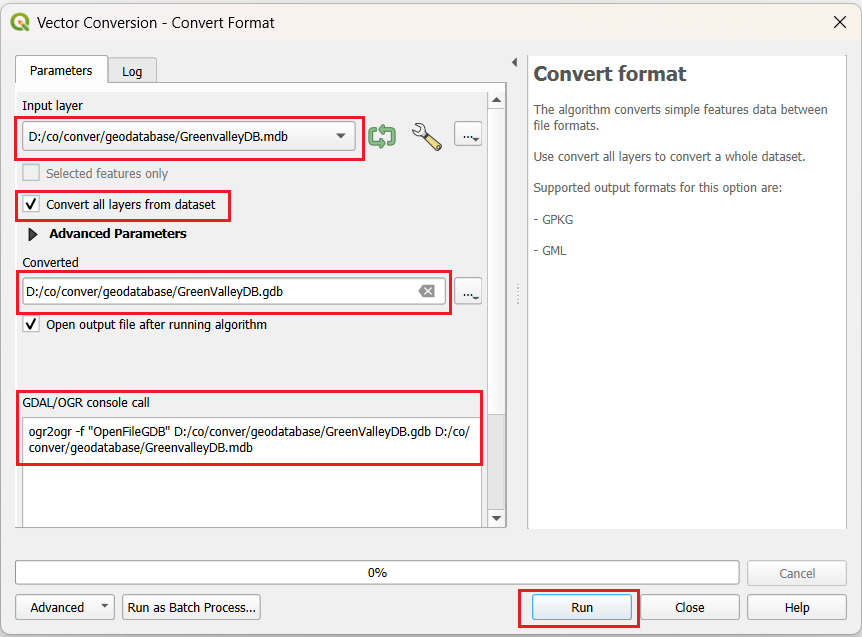
\includegraphics[width=0.75\textwidth,height=\textheight]{images/conversion_formatos/convert_format_qgis_mdb_gdb.png}

}

\caption{\label{fig-convert-format}Uso del algoritmo Convert format de
GDAL para transformar bases de datos enteras.}

\end{figure}%

\subsubsection{Método C: Creación y arrastre desde el panel del
navegador}\label{muxe9todo-c-creaciuxf3n-y-arrastre-desde-el-panel-del-navegador}

\begin{itemize}
\tightlist
\item
  \textbf{Objetivo:} Crear una File Geodatabase vacía desde cero y
  migrar las capas visualmente arrastrándolas entre directorios.
\item
  \textbf{Herramientas:} Panel del navegador (\texttt{Browser}) en QGIS.
\item
  \textbf{Proceso:}

  \begin{enumerate}
  \def\labelenumi{\arabic{enumi}.}
  \item
    Haga clic derecho sobre la carpeta de destino
    (\texttt{geodatabase}), seleccione \texttt{New} (Nuevo) y luego
    \texttt{ESRI\ FileGeodatabase...} para crear la base vacía.
  \item
    Despliegue el contenido del archivo \texttt{GreenvalleyDB.mdb} en el
    navegador, seleccione todas sus capas (con la tecla \emph{Shift}),
    arrástrelas y suéltelas sobre la nueva base de datos.
  \item
    Utilice el botón de refrescar para confirmar la copia de los datos.

    \begin{itemize}
    \item
      \textbf{Datos de entrada:} Capas internas de
      \texttt{GreenvalleyDB.mdb} (ej. \texttt{buildings\_point},
      \texttt{flood\_polygon}, etc.).
    \item
      \textbf{Datos de salida:} \texttt{GrenValleyDB2.gdb} (almacenado
      en la carpeta \texttt{geodatabase}).
    \end{itemize}
  \end{enumerate}
\end{itemize}

\begin{figure}

\centering{

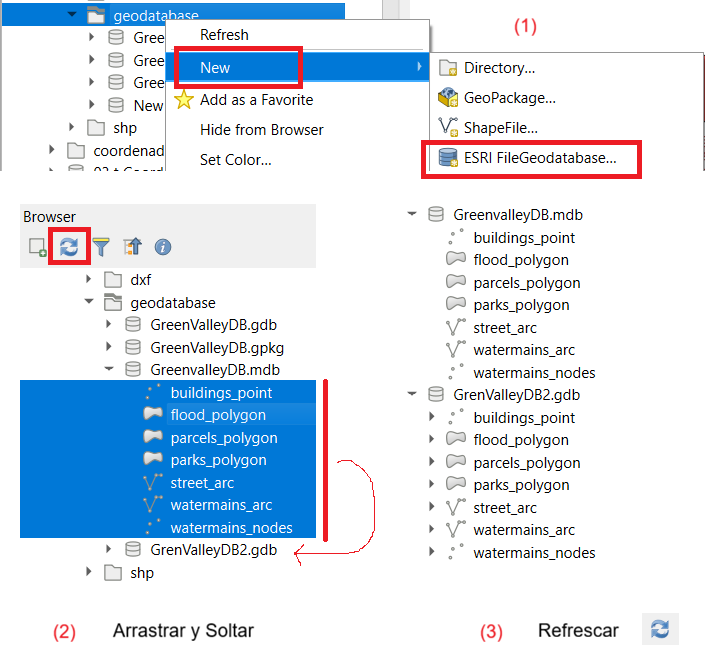
\includegraphics[width=0.5\textwidth,height=\textheight]{images/conversion_formatos/arrasrtar_soltar_qgis_mdb_gdb.png}

}

\caption{\label{fig-drag-drop-gdb}Proceso de creación, arrastre y
copiado de datos mediante el navegador de QGIS.}

\end{figure}%

\subsection{Ejercicio 2: Exportación de capas vectoriales a formatos CAD
(DXF)}\label{ejercicio-2-exportaciuxf3n-de-capas-vectoriales-a-formatos-cad-dxf}

\begin{itemize}
\item
  \textbf{Objetivo:} Exportar capas vectoriales a formatos
  estandarizados de diseño asistido por computadora para facilitar el
  intercambio con software de ingeniería.
\item
  \textbf{Herramientas:}

  \begin{itemize}
  \tightlist
  \item
    \textbf{ArcGIS Pro:} \texttt{Conversion\ Tools} (Herramientas de
    conversión) -\textgreater{} \texttt{To\ CAD} (A CAD) -\textgreater{}
    \texttt{Export\ to\ CAD} (Exportar a CAD).
  \item
    \textbf{QGIS:} Menú \texttt{Project} (Proyecto) -\textgreater{}
    \texttt{Import/Export} (Importar/Exportar) -\textgreater{}
    \texttt{Export\ project\ to\ DXF} (Exportar proyecto a DXF) o desde
    la caja de herramientas GDAL \texttt{Export\ layers\ to\ DXF}
    (Exportar capas a DXF).
  \end{itemize}
\item
  \textbf{Datos de entrada:} Capas vectoriales almacenadas en
  \texttt{GreenValleyDB.gdb} (por ejemplo, las capas urbanas o de
  infraestructura).
\item
  \textbf{Datos de salida:} Archivos espaciales CAD en formato
  \texttt{.dxf} (con 6 decimales de precisión en sus coordenadas) dentro
  de la carpeta \texttt{dxf}.
\end{itemize}

\begin{figure}

\centering{

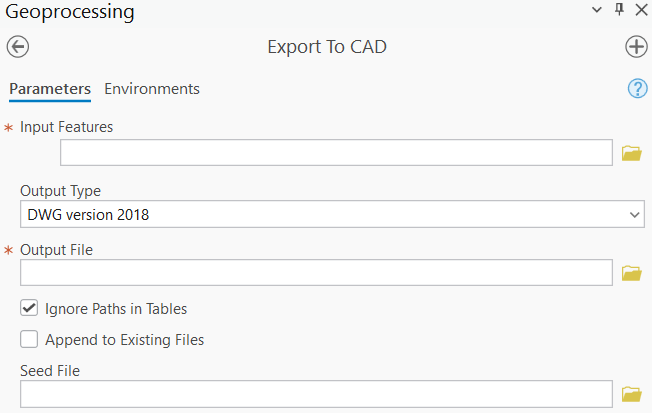
\includegraphics[width=0.5\textwidth,height=\textheight]{images/conversion_formatos/export_to_cad_pro.png}

}

\caption{\label{fig-export_to_cad_pro}Herramienta Export to CAD
(Exportar a CAD) en ArcGIS Pro.}

\end{figure}%

\begin{quote}
\textbf{Tip avanzado para ArcGIS Pro:} Si exportas entidades de puntos y
deseas que se representen con una simbología específica de AutoCAD,
puedes crear un campo de texto llamado \textbf{\texttt{RefName}} en tu
tabla de atributos y escribir allí el nombre del bloque. Al exportar
usando un archivo DWG de plantilla (Seed file) que contenga dichos
bloques, ArcGIS los insertará automáticamente en la posición de cada
punto.
\end{quote}

\begin{figure}

\centering{

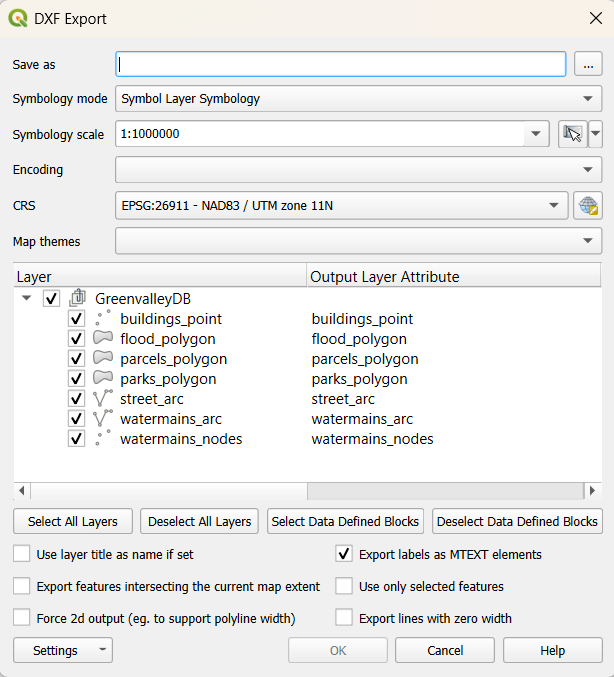
\includegraphics[width=0.5\textwidth,height=\textheight]{images/conversion_formatos/dxf_export_qgis.png}

}

\caption{\label{fig-dxf_export_qgis}Herramienta DXF Export (Exportar a
DXF) en QGIS.}

\end{figure}%

\begin{figure}

\centering{

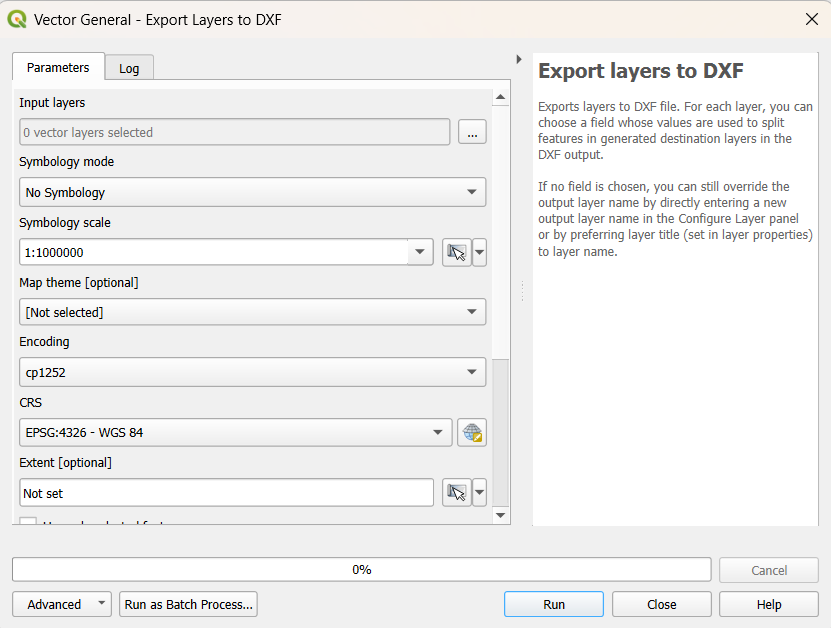
\includegraphics[width=0.5\textwidth,height=\textheight]{images/conversion_formatos/export_layers_dxf_qgis.png}

}

\caption{\label{fig-dxf_export_qgis}Herramienta Export Layers to DXF
(Exportar Capas a DXF) en QGIS.}

\end{figure}%

\subsubsection{Caso de estudio avanzado en ArcGIS Pro: Simbología
geológica con atributos
automáticos}\label{caso-de-estudio-avanzado-en-arcgis-pro-simbologuxeda-geoluxf3gica-con-atributos-automuxe1ticos}

A continuación, se detalla un flujo de trabajo para exportar puntos de
datos estructurales (buzamientos geológicos) logrando que la simbología
geométrica (el bloque) y el texto asociado (el ángulo de buzamiento) se
generen automáticamente dentro del archivo CAD resultante, respetando
los estándares de diseño de una plantilla predefinida.

\begin{itemize}
\tightlist
\item
  \textbf{Datos de entrada GIS:} Shapefile de puntos
  \texttt{buz\_final.shp} (en carpeta /datos/shapefile\_dxf/) que
  representa ubicaciones de medidas de buzamiento.
\item
  \textbf{Configuración de la tabla GIS:} La tabla de atributos incluye
  tanto campos reservados de CAD (especificados en la
  \href{https://pro.arcgis.com/en/pro-app/latest/help/data/cad/reserved-cad-fields-for-dwg-and-dxf-files.htm}{ayuda
  oficial} de Esri) como campos personalizados de atributo.

  \begin{itemize}
  \tightlist
  \item
    \textbf{\texttt{RefName}}: Campo reservado de texto que especifica
    el nombre exacto del bloque CAD a insertar (por ejemplo el bloque
    ``\textbf{100000}'').
  \item
    \textbf{\texttt{DIP}}: Campo personalizado que contiene el valor
    numérico del ángulo de buzamiento (aplica para el bloque
    \textbf{100000}).
  \end{itemize}
\item
  \textbf{Archivo de plantilla CAD (Seed file):}
  \texttt{DatosEstructuralesBloques\_ATTDEF.dwg}. Este archivo debe
  contener la definición del bloque ``\textbf{100000}'' (y todos los
  demás bloques definidos en el campo \texttt{RefName}), y vitalmente,
  dentro de ese bloque debe existir una definición de atributo
  (\textbf{ATTDEF}) con la etiqueta (\textbf{Tag}) exacta
  ``\textbf{DIP}''.
\end{itemize}

\begin{figure}

\centering{

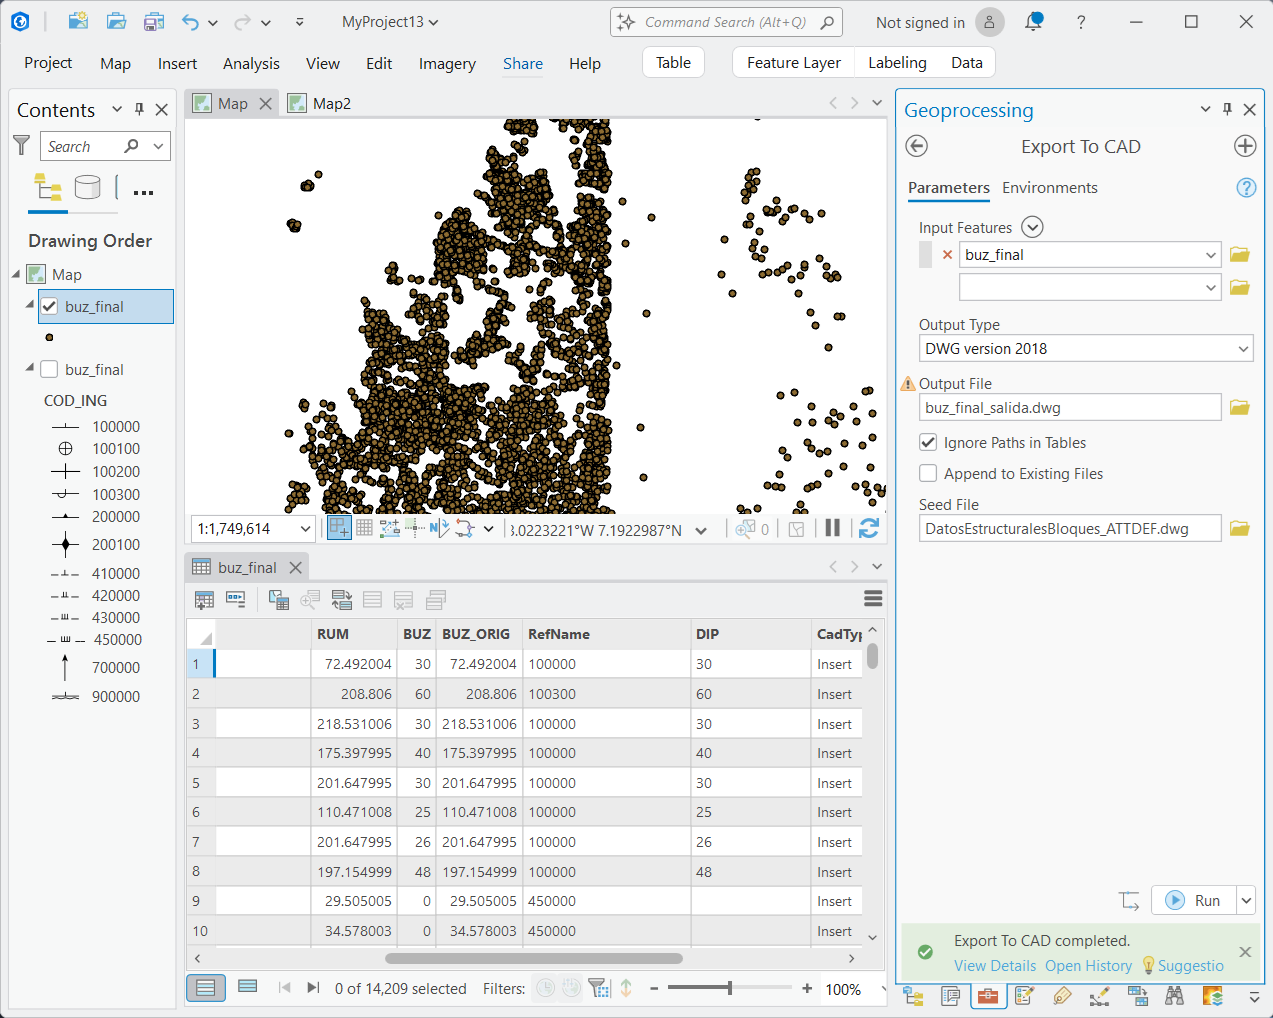
\includegraphics[width=1\textwidth,height=\textheight]{images/conversion_formatos/export_to_cad_pro_seed_file_reserved_fields.png}

}

\caption{\label{fig-cad-avanzado}Visualización de la tabla de atributos
de \texttt{buz\_final.shp} con campos reservados (ej: \texttt{RefName},
\texttt{CadType}, \texttt{ScaleX}, \ldots) y personalizados
(\texttt{DIP}) configurados para su exportación avanzada a CAD usando
una plantilla (\texttt{Seed\ file}) que soporta definiciones de
atributos (\texttt{ATTDEF}).}

\end{figure}%

\textbf{Explicación del mecanismo técnico:}

Cuando se ejecuta la herramienta \texttt{Export\ to\ CAD} (Exportar a
CAD) en ArcGIS Pro:

\begin{enumerate}
\def\labelenumi{\arabic{enumi}.}
\tightlist
\item
  \textbf{Lectura de geometría:} ArcGIS lee la coordenada espacial XY
  del punto GIS.
\item
  \textbf{Identificación del bloque:} Lee el campo reservado
  \texttt{RefName} (ej: valor ``\textbf{100000}'') y localiza la
  definición de ese bloque dentro del archivo \texttt{seed} (plantilla).
\item
  \textbf{Inserción del bloque:} Inserta el bloque geométrico
  ``\textbf{100000}'' en la coordenada correspondiente en el DWG
  resultante.
\item
  \textbf{Mapeo dinámico de atributos:} El motor de exportación GIS
  busca coincidencias exactas entre los nombres de los campos
  personalizados de la tabla GIS y las etiquetas (\textbf{Tags}) de los
  atributos (\textbf{ATTDEF}) definidos \emph{dentro} del bloque CAD. Al
  encontrar una coincidencia exacta para ``\textbf{DIP}'', transfiere
  automáticamente el valor del campo GIS al texto del atributo del
  bloque insertado.
\end{enumerate}

\textbf{Resultado:}

En el archivo DWG creado, los puntos GIS ya no serán puntos simples,
sino referencias de bloques complejos. La simbología geométrica será
correcta y aparecerá un texto mostrando el ángulo de buzamiento en la
posición, rotación y estilo definidos en la plantilla CAD, sin necesidad
de generar textos adicionales manualmente en el DWG.

\begin{tcolorbox}[enhanced jigsaw, opacityback=0, left=2mm, colbacktitle=quarto-callout-important-color!10!white, leftrule=.75mm, breakable, titlerule=0mm, rightrule=.15mm, bottomrule=.15mm, arc=.35mm, colback=white, colframe=quarto-callout-important-color-frame, opacitybacktitle=0.6, toptitle=1mm, title=\textcolor{quarto-callout-important-color}{\faExclamation}\hspace{0.5em}{Evolución de la interoperabilidad CAD - GIS hacia entornos BIM}, bottomtitle=1mm, toprule=.15mm, coltitle=black]

Es fundamental aclarar que la interoperabilidad entre los mundos del
diseño de infraestructura (CAD) y el análisis espacial (GIS) ha
evolucionado drásticamente más allá de la simple exportación de líneas y
polígonos en formatos tradicionales.

En la actualidad, esta integración de alto nivel se rige por la
metodología \textbf{BIM (Building Information Modeling)}. Para proyectos
de ingeniería avanzada (como los generados en AutoCAD Civil 3D,
Infraworks o Revit), el estándar universal de intercambio abierto es el
formato \textbf{IFC (Industry Foundation Classes)}.

Adicionalmente, motores SIG modernos como ArcGIS Pro cuentan con
conectores nativos que integran directamente archivos
\textbf{\texttt{.rvt}} y modelos de \textbf{Civil 3D}. Este salto
tecnológico es crucial porque \textbf{facilita la lectura directa} de
los elementos constructivos sin requerir conversiones intermedias
destructivas, conservando intacta la riqueza de los metadatos de
ingeniería y permitiendo una \textbf{visualización 3D nativa} para el
análisis volumétrico y espacial dentro del entorno geográfico.

\end{tcolorbox}

\subsection{Ejercicio 3: Despliegue optimizado de una imagen escaneada
con 3 bandas
(RGB)}\label{ejercicio-3-despliegue-optimizado-de-una-imagen-escaneada-con-3-bandas-rgb}

\textbf{Nota técnica:} Las imágenes ráster escaneadas (como mapas o
fotografías aéreas antiguas) ya poseen una representación visual final
destinada al ojo humano. A diferencia de las bandas de satélite crudas,
un escaneo RGB no requiere estiramientos de contraste agresivos que
alteren sus colores originales. Sin embargo, los SIG modernos a menudo
aplican mejoras dinámicas automáticas al cargar cualquier ráster, lo que
puede ``lavar'' o saturar los colores del escaneo.

El objetivo de este ejercicio es configurar el motor de visualización
para respetar los valores de color originales del escaneo y optimizar la
legibilidad del texto mediante técnicas de remuestreo dinámico en
\textbf{ArcGIS Pro} y \textbf{QGIS}.

\begin{itemize}
\tightlist
\item
  \textbf{Objetivo:} Visualizar correctamente un mapa escaneado
  multibanda, verificando el mapeo RGB y ajustando las opciones de
  estiramiento y remuestreo para maximizar la legibilidad visual sin
  alterar la radiometría original del escaneo.
\item
  \textbf{Herramientas:} Funciones de visualización y simbología ráster
  en \textbf{ArcGIS Pro} y \textbf{QGIS}.
\item
  \textbf{Datos de entrada:} Imagen ráster escaneada
  \texttt{caleriza.tif} (GeoTIFF compuesto de 3 bandas, almacenado en la
  carpeta \texttt{datos}).
\item
  \textbf{Datos de salida:} No aplica (los cambios se visualizan en vivo
  en el lienzo del mapa).
\end{itemize}

\subsubsection{Flujo de trabajo en ArcGIS Pro}

ArcGIS Pro ofrece un control visual inmediato desde la cinta de opciones
(Ribbon). Al cargar la imagen \texttt{caleriza.tif}, el software mapea
automáticamente las bandas 1, 2 y 3 a los canales Rojo, Verde y Azul. El
desafío es que a menudo aplica un estiramiento de contraste
predeterminado (ej. \emph{Percent Clip}) que distorsiona el color real
del mapa escaneado.

El proceso correcto para un escaneo es eliminar el estiramiento y
mejorar la nitidez al hacer zoom:

\textbf{1. Verificación de bandas y eliminación del estiramiento de
contraste:}

Haga clic sobre la capa ráster. En el panel \texttt{Raster\ Layer} (Capa
Raster), sección ~\texttt{Symbology} (Simbología), verifique que la
simbología de despliegue sea \texttt{RGB}. Alternativamente: Cambié el
\texttt{Stretch\ type} (Tipo de estiramiento) a \texttt{None} (Ninguno).
Esto asegura que el SIG visualice los valores de color exactos que
fueron escaneados.

\begin{figure}

\centering{

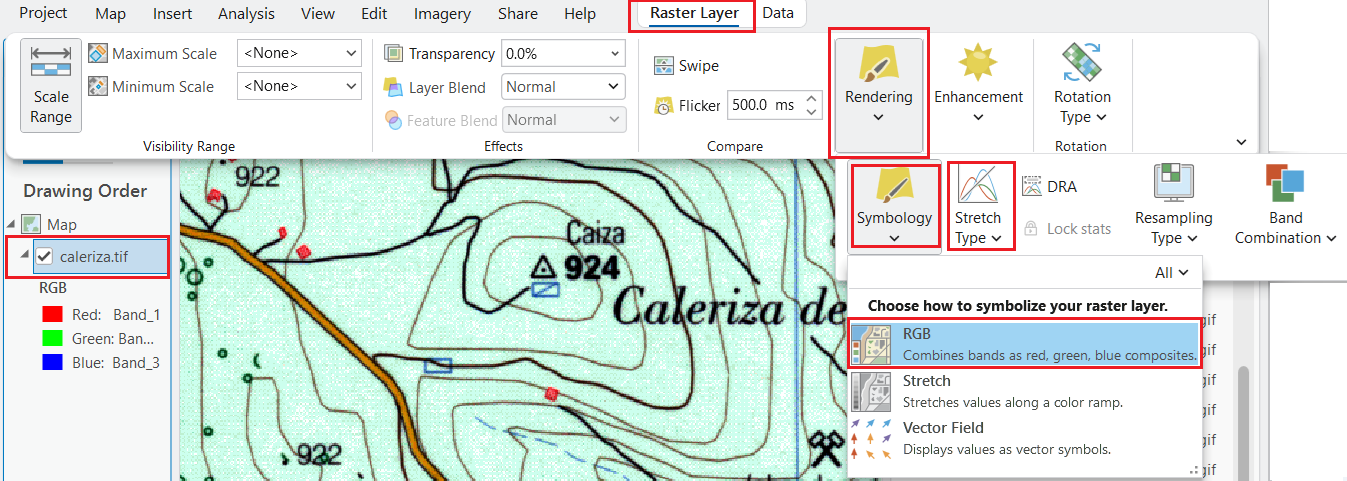
\includegraphics[width=1\textwidth,height=\textheight]{images/conversion_formatos/rgb_visualization_imagen_escaneada_pro_1.png}

}

\caption{\label{fig-pro-symbology-none}Panel \texttt{Raster\ Layer}
(Capa Raster), sección \texttt{Symbology} (Simbología) en ArcGIS Pro
configurando el renderizado RGB.}

\end{figure}%

\textbf{2. Optimización dinámica de la visualización (Cinta de
opciones):}

Active la pestaña \texttt{Raster\ Layer} (Capa ráster) -\textgreater{}
grupo \texttt{Rendering} (Renderizado) en la cinta de opciones. Aquí
puede controlar la visualización de forma global.

\begin{itemize}
\item
  Verifique que la opción \texttt{DRA} (Dynamic Range Adjustment
  {[}Ajuste de rango dinámico{]}) esté desactivada, ya que esta
  herramienta recalcula el contraste constantemente al navegar, lo que
  no se desea en un mapa escaneado.
\item
  Verifique que el \texttt{Resampling\ Type} (Tipo de Remuestreo) está
  establecido por defecto a \texttt{Nearest\ Neighbor} (Vecino mas
  Cercano) y observe que el despliegue del mapa escaneado no es nítido.
  Por defecto, al hacer zoom sobre un ráster (especialmente texto
  escaneado), ArcGIS Pro utiliza el método \texttt{Nearest\ Neighbor},
  lo que provoca una visualización ``pixelada'' o escalonada.
\end{itemize}

\begin{figure}

\centering{

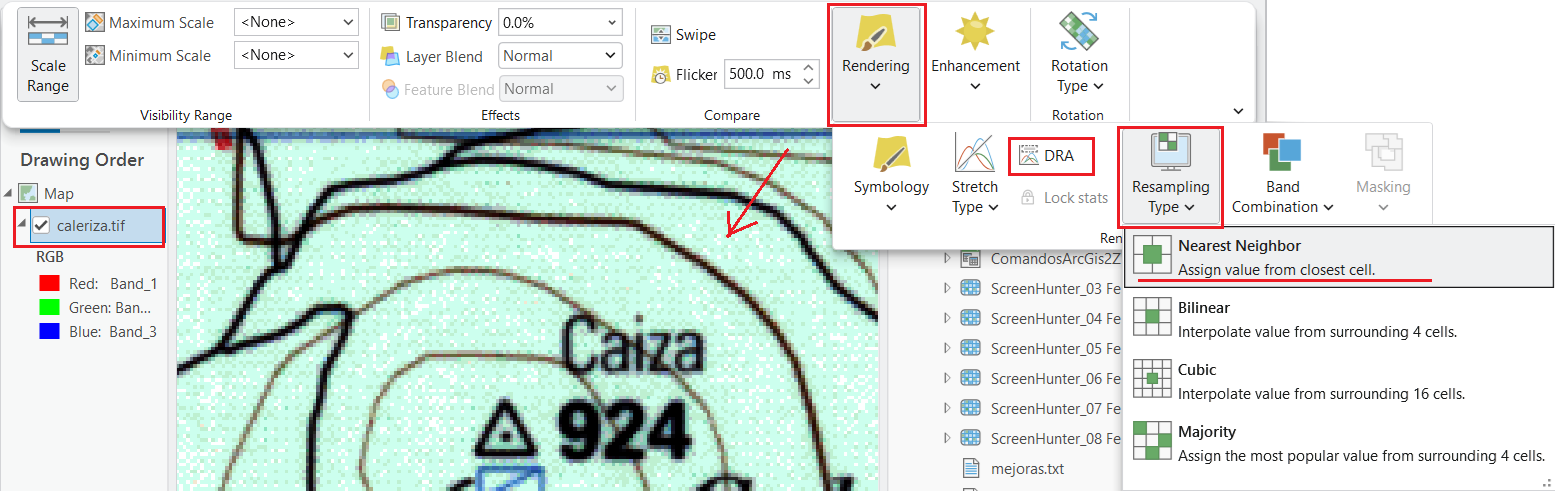
\includegraphics[width=1\textwidth,height=\textheight]{images/conversion_formatos/rgb_visualization_imagen_escaneada_pro_2.png}

}

\caption{\label{fig-pro-rendering-ribbon}Uso de la pestaña
\texttt{Raster\ Layer} (Capa ráster) -\textgreater{} grupo
\texttt{Rendering} (Renderizado) en ArcGIS Pro para verificar el tipo de
remuestreo y sus efectos en el despliegue de la imagen.}

\end{figure}%

\textbf{3. Mejora de legibilidad mediante remuestreo:}

Para mejorar drásticamente la lectura de textos y líneas finas en un
escaneo, cambie el \texttt{Resampling\ Type} (Tipo de remuestreo)
dinámico a \texttt{Bilinear} (Bilineal) o \texttt{Cubic} (Cúbico) en la
pestaña \texttt{Raster\ Layer} (Capa ráster) -\textgreater{} grupo
\texttt{Rendering} (Renderizado). Esto suaviza la imagen al vuelo sin
alterar el archivo original, permitiendo leer el mapa con mayor nitidez.

\begin{figure}

\centering{

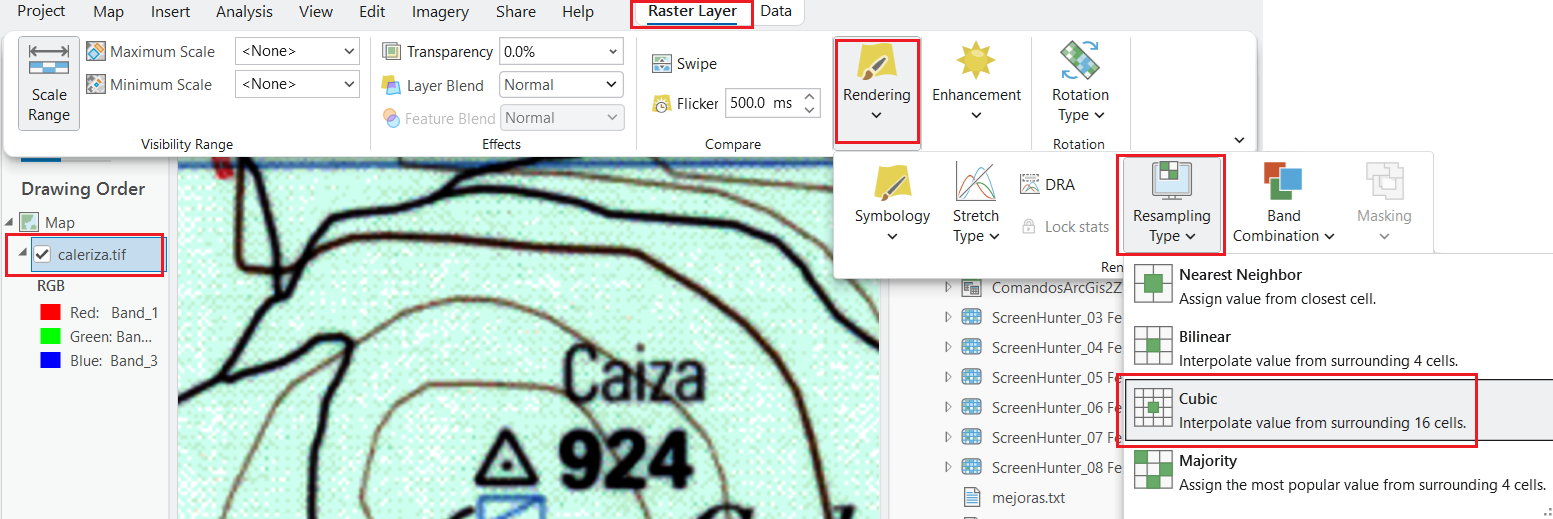
\includegraphics[width=1\textwidth,height=\textheight]{images/conversion_formatos/rgb_visualization_imagen_escaneada_pro_3.png}

}

\caption{\label{fig-pro-resampling-compare}Comparación visual del efecto
del remuestreo dinámico en ArcGIS Pro usando \texttt{Cubic} (Cúbico).}

\end{figure}%

\subsubsection{Flujo de trabajo en QGIS}

En QGIS, el proceso es más directo y se centraliza en la ventana de
propiedades de la capa.

\textbf{1. Configuración de simbología y remuestreo:}

Haga doble clic (o clic derecho) sobre la capa \texttt{caleriza.tif}
-\textgreater{} pestaña \texttt{Symbology} (Simbología).

\begin{itemize}
\tightlist
\item
  En la sección \texttt{Band\ Rendering} (Renderizado de Banda),
  verifique que el \texttt{Render\ type} (Tipo de renderizado) sea
  \texttt{Multiband\ Color} (Color Multibanda).
\item
  En la sección \texttt{Band\ Rendering} (Renderizado de Banda), luego
  en \texttt{Contrast\ enhancement} (Mejora de contraste), seleccione
  \texttt{No\ Enhancement} (Sin mejora) para respetar los colores
  originales del escaneo.
\end{itemize}

\begin{figure}

\centering{

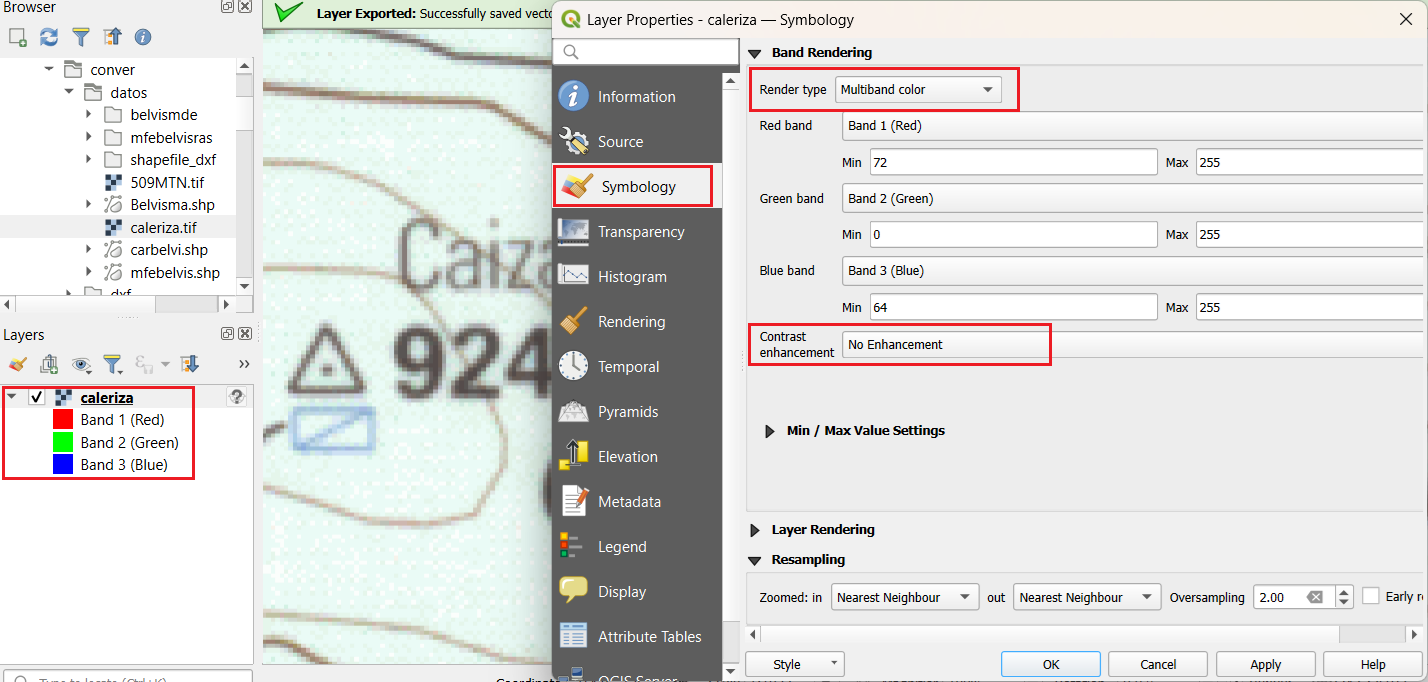
\includegraphics[width=1\textwidth,height=\textheight]{images/conversion_formatos/rgb_visualization_imagen_escaneada_qgis_1.png}

}

\caption{\label{fig-qgis-symbology}Panel de \texttt{Symbology}
(Simbología) en QGIS configurando el renderizado ráster
\texttt{Multiband\ color} (Color multibanda) y \texttt{No\ Enhancement}
(sin estiramiento)}

\end{figure}%

\textbf{2. Optimización de visualización:}

Al igual que en ArcGIS Pro, \texttt{Nearest\ Neighbor} (Vecino más
cercano) pixelará el texto al hacer zoom. En la misma pestaña de
\texttt{Symbology} (Simbología), localice las opciones de
\texttt{Resampling} (Remuestreo). A diferencia de otros programas, QGIS
divide el remuestreo en dos configuraciones independientes para
optimizar los cálculos matemáticos según el nivel de acercamiento:

\begin{itemize}
\tightlist
\item
  \textbf{\texttt{Zoomed\ in} (Acercar):} Se activa cuando hace un
  acercamiento más allá de la resolución nativa del ráster (un solo
  píxel de la imagen debe representarse usando varios píxeles de su
  monitor). Para evitar que los textos y líneas se vean como bloques
  cuadrados, cambie este método a \texttt{Bilinear} (Bilineal) o
  \texttt{Cubic} (Cúbico), algoritmos que interpolan transiciones suaves
  entre los colores.
\item
  \textbf{\texttt{Zoomed\ out} (Alejar):} Se activa cuando se aleja la
  vista (múltiples píxeles de la imagen original se comprimen para caber
  en un solo píxel de su monitor). En este caso, cambie el método
  también a \texttt{Bilinear} (Bilineal) o \texttt{Cubic} (Cúbico), los
  cuales aplican cálculos de interpolación entre los píxeles
  circundantes para evitar la pérdida de líneas finas o el efecto de
  distorsión óptica (\emph{aliasing}) en el mapa escaneado.
\end{itemize}

\begin{figure}

\centering{

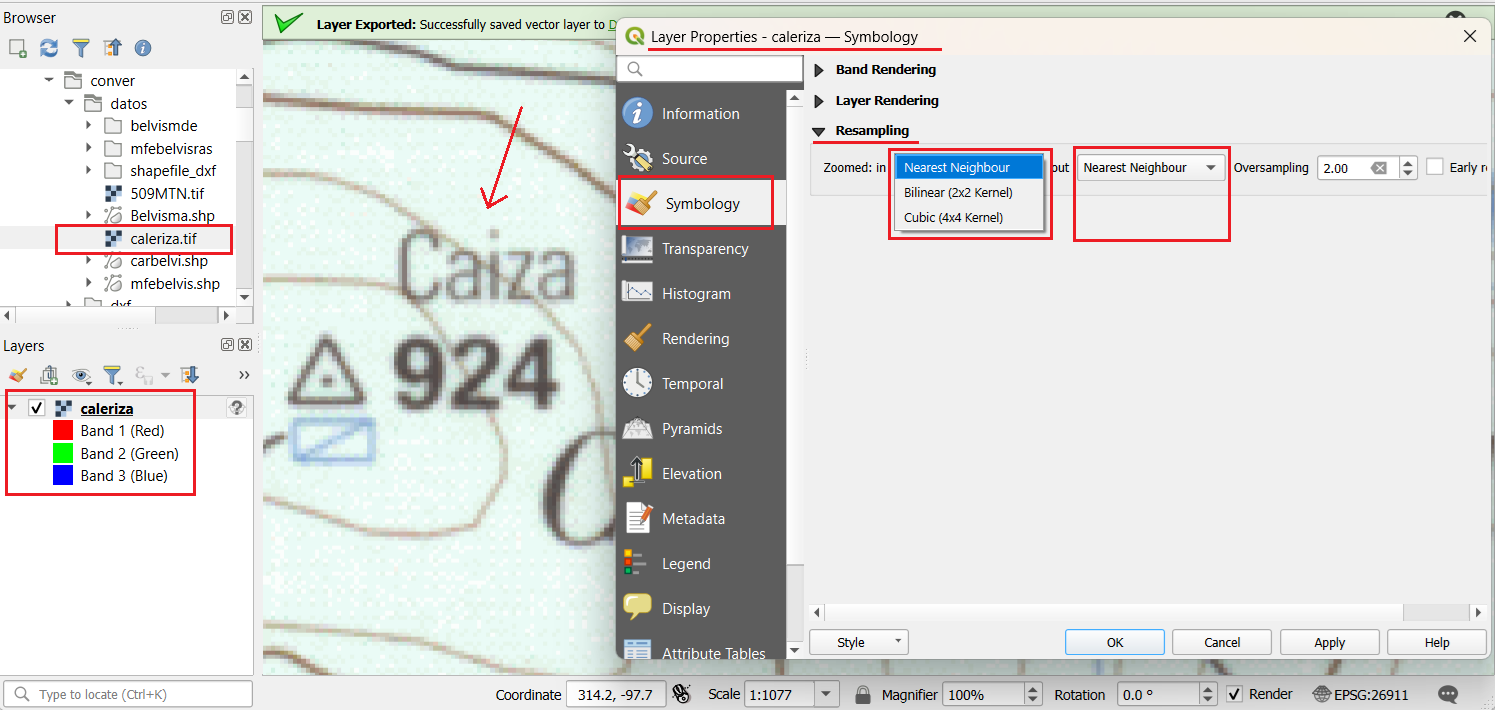
\includegraphics[width=1\textwidth,height=\textheight]{images/conversion_formatos/rgb_visualization_imagen_escaneada_qgis_2.png}

}

\caption{\label{fig-qgis-symbology-resampling}Panel de
\texttt{Symbology} (Simbología) en QGIS configurando el renderizado
ráster para ajustar las opciones de \texttt{Resampling} (Remuestreo)
dinámico para optimizar el despliegue visual.}

\end{figure}%

\subsection{Ejercicio 4: Georreferenciar una imagen con archivo
world}\label{ejercicio-4-georreferenciar-una-imagen-con-archivo-world}

Las imágenes que poseen una distorsión poco significativa en su
cuadrícula para el trabajo a realizar, por ejemplo, las que se adquieren
mediante el escaneo de mapas, o de imágenes en general que han perdido
su referenciación terrestre tras haber sido rectificadas, pueden ser
fácilmente georreferenciadas mediante la incorporación de un archivo de
texto adjunto con estructura interna ``world'' y extensión con final en
``w'' (ej. \texttt{.tfw} para imágenes \texttt{.tif}). Para realizar
esta operación es necesario, previamente, conocer el número de píxeles
de la imagen, además de las coordenadas de un punto y el tamaño que en
la realidad le corresponde a cada píxel (resolución espacial).

\textbf{Descripción de los datos (\texttt{5O9MTN.tif}):} Antes de
proceder con la georreferenciación, es importante entender la naturaleza
del archivo con el que vamos a trabajar. El nombre
\textbf{\texttt{5O9MTN}} hace referencia a la \textbf{Hoja 509} (zona de
Alcalá de Henares, Madrid) del \textbf{Mapa Topográfico Nacional (MTN)}
de España. Técnicamente, es una composición de tres bandas capturadas
por el sensor TM del satélite Landsat, recortada para coincidir con los
límites de esa hoja cartográfica oficial. Debido a su origen y
ubicación, el Sistema de Referencia de Coordenadas (CRS) probable de
esta imagen es \textbf{ED50 / UTM zone 30N (EPSG:23030)}, un estándar
histórico español cuyas unidades de medida métrica son los
\textbf{metros}.

\textbf{Paso 1: Cómo calcular el tamaño de una imagen}

Cargue la imagen \texttt{5O9MTN.tif} (que se encuentra en la carpeta de
datos) en \textbf{ArcGIS Pro} o \textbf{QGIS}.

Para saber las características de la imagen \texttt{5O9MTN.tif}, haga
clic sobre el nombre de la capa con el botón derecho del ratón y abra
\texttt{Properties} (Propiedades):

\subsubsection{\texorpdfstring{\textbf{ArcGIS Pro}}{ArcGIS Pro}}

\begin{itemize}
\tightlist
\item
  En \textbf{ArcGIS Pro}, en la ventana de propiedades de la capa,
  active la sección \texttt{Source} (Fuente) y expanda
  \texttt{Raster\ Information} (Información del ráster).
\end{itemize}

\begin{figure}

\centering{

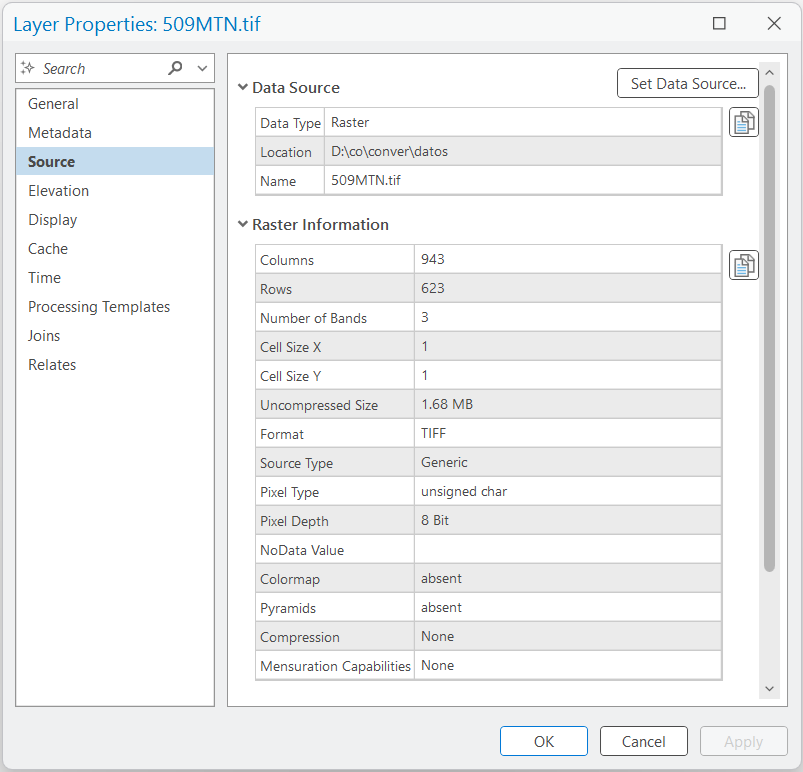
\includegraphics[width=0.8\textwidth,height=\textheight]{images/conversion_formatos/raster_information_pro.png}

}

\caption{\label{fig-arcgis-raster-properties}Información de la capa
raster en ArcGIS Pro.}

\end{figure}%

\subsubsection{\texorpdfstring{\textbf{QGIS}}{QGIS}}

\begin{itemize}
\tightlist
\item
  En \textbf{QGIS}, en la ventana de propiedades de la capa, active la
  sección \texttt{Information} (Información).
\end{itemize}

\begin{figure}

\centering{

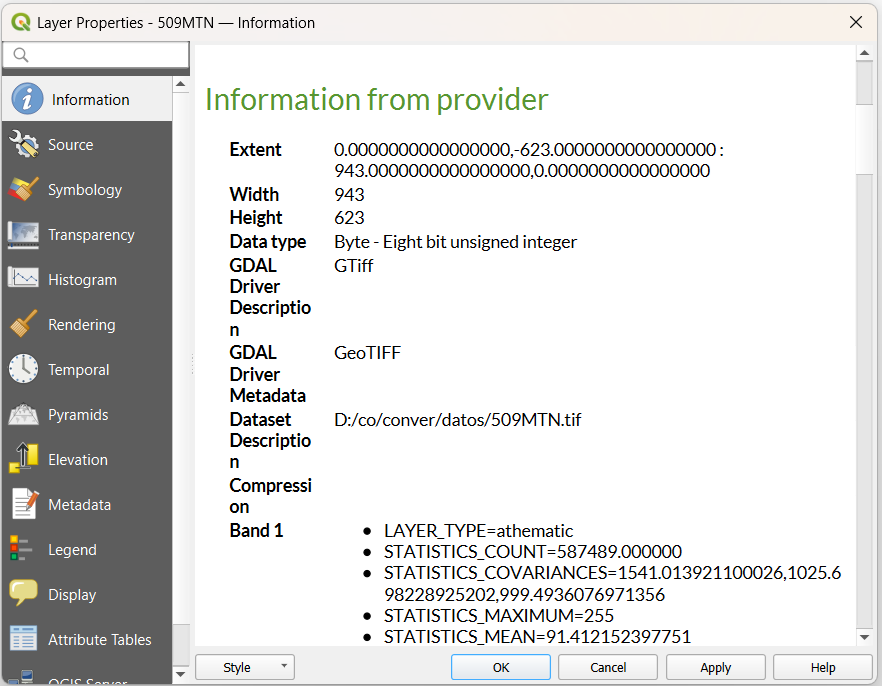
\includegraphics[width=0.8\textwidth,height=\textheight]{images/conversion_formatos/raster_information_qgis.png}

}

\caption{\label{fig-qgis-raster-properties}Información de la capa raster
en QGIS.}

\end{figure}%

La información que nos ofrece nos permite conocer el número de filas y
columnas que la componen, el tipo de datos admitidos en cada celda
(\texttt{Pixel\ Depth} {[}Profundidad del Pixel{]} y \texttt{Data\ Type}
{[}Tipo de Dato{]}); y si existen compresiones, pirámides, etc.

En el ejemplo señalado, la imagen posee 943 columnas por 623 filas, esto
es, 587.489 celdas. El tamaño del píxel estaría en función de las
coordenadas en las que se inscribe y está medido por las unidades de
medida del mapa, por lo que no es un dato relevante hasta que no se
produzca la georreferenciación.

\textbf{Paso 2: Referenciar una imagen con documento ``world'' adjunto}

Para entender cómo se georreferencia una imagen, primero debemos
comprender la relación entre el \textbf{Espacio de Imagen} (donde el
origen \texttt{0,0} está en la esquina superior izquierda de la pantalla
y se mide en píxeles hacia abajo y a la derecha) y el \textbf{Espacio de
Coordenadas} (el mundo real, medido en metros o grados, donde el eje Y
crece hacia arriba).

Observe la siguiente gráfica que ilustra esta relación:

\begin{figure}

\centering{

\includegraphics[width=0.85\textwidth,height=\textheight]{images/conversion_formatos/image_077aba.png}

}

\caption{\label{fig-espacio-imagen-coordenadas}Relación geométrica entre
el Espacio de Imagen (Píxeles) y el Espacio de Coordenadas (Metros). Se
destacan las dimensiones del píxel (A, E) y las coordenadas de origen
(C, F).}

\end{figure}%

Para referenciar la imagen tendremos que crear un archivo de texto (con
cualquier procesador de texto plano o el Bloc de notas) que le traduzca
al SIG cómo pasar del \emph{Espacio de Imagen} al \emph{Espacio de
Coordenadas}. Este archivo debe contener exactamente seis filas de datos
(más una en blanco al final) correspondientes a los parámetros de la
gráfica anterior:

\begin{enumerate}
\def\labelenumi{\arabic{enumi}.}
\tightlist
\item
  \textbf{La primera fila (Variable A):} Hace referencia al tamaño real
  de los píxeles en dirección X (\texttt{World\ coordinate}
  {[}Coordenada del mundo{]}). Siempre es positivo porque X aumenta
  hacia la derecha en ambos espacios. Es decir, \textbf{30} metros (cada
  píxel equivale a 30 metros de ancho en el terreno).
\item
  \textbf{La segunda fila:} Rotación respecto al eje Y. Como la imagen
  no está rotada, el valor es \textbf{0}.
\item
  \textbf{La tercera fila:} Rotación respecto al eje X. Como la imagen
  no está rotada, el valor es \textbf{0}.
\item
  \textbf{La cuarta fila (Variable E):} Es el tamaño real del píxel en
  dirección Y. Este valor es \textbf{siempre negativo} (en este caso
  \textbf{-30} metros) porque en la imagen las filas crecen hacia abajo,
  pero en el mundo real las coordenadas Y disminuyen hacia abajo.
\item
  \textbf{La quinta fila (Variable C):} Es la coordenada \textbf{X}
  exacta del centro del primer píxel superior izquierdo. En este caso
  X=\textbf{427900}.
\item
  \textbf{La sexta fila (Variable F):} Es la coordenada \textbf{Y}
  exacta del centro del primer píxel superior izquierdo. En este caso
  Y=\textbf{4520833}.
\end{enumerate}

Al importar el ráster, el programa identifica automáticamente sus
dimensiones. Al integrar esta información con los seis parámetros
descritos en el archivo \texttt{5O9MTN.tfw}, el software calcula la
posición espacial de todos los demás píxeles sin deformar la imagen.

\textbf{Nota sobre la integridad de los datos:} Evite manipular
manualmente los valores numéricos del archivo world para intentar
``ajustar'' o corregir visualmente una imagen que se ve desplazada o
torcida; esto solo provocará deformaciones geométricas asimétricas
(achatamiento o estiramiento). Si la imagen requiere ajustes de posición
o corrección de distorsiones, utilice las herramientas de
georreferenciación de su software SIG para garantizar la precisión
espacial.

Abra el Bloc de notas de su sistema operativo e introduzca los datos
correspondientes (recuerde dejar una fila en blanco al final):

\begin{figure}

\centering{

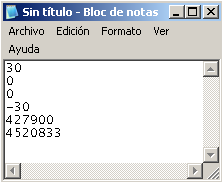
\includegraphics[width=0.3\textwidth,height=\textheight]{images/conversion_formatos/archivo_5O9MTN.tfw.png}

}

\caption{\label{fig-world-file}Contenido exacto del archivo de texto
world creado en el Bloc de notas.}

\end{figure}%

Ahora guarde este documento en la misma carpeta donde se ubica la imagen
\texttt{5O9MTN.tif}, asignándole el nombre \texttt{5O9MTN.tfw}. Es
fundamental elegir en el cuadro de diálogo la opción Tipo
\texttt{All\ Files} (Todos los archivos) en lugar de
\texttt{Text\ Documents\ (*.txt)} (Documentos de texto), por lo que
llevará su mismo nombre base, pero con distinta extensión. Si el archivo
apareciera con la extensión \texttt{.txt}, habría que cambiarla
manualmente por \texttt{.tfw}, con la ``w'' alusiva a las coordenadas
reales (World coordinate).

\textbf{Ajuste de las unidades del mapa (Data Frame / Lienzo):} El
archivo \emph{world} (\texttt{.tfw}) es agnóstico; solo le dice al
software que el píxel mide ``30 unidades'', pero no especifica si son
metros, pies o grados. Si el mapa donde carga la imagen está configurado
por defecto en grados decimales o pies, la imagen se dibujará con un
tamaño incorrecto y no coincidirá espacialmente con ninguna capa base.

Para que el archivo \texttt{.tfw} funcione correctamente al cargar la
imagen, primero debemos asegurar que el mapa base utilice
\textbf{metros}.

\begin{itemize}
\tightlist
\item
  \textbf{En ArcGIS Pro:} Haga clic derecho sobre el nombre del mapa en
  el panel \texttt{Contents} (Contenido), elija \texttt{Properties}
  (Propiedades) y en la pestaña \texttt{Coordinate\ Systems} (Sistemas
  de coordenadas) asigne el sistema \textbf{European Datum 1950 UTM Zone
  30N} (23030). Alternativamente puede cargar el mapa base
  \texttt{Imagery} (menú \texttt{Map} -\textgreater{} \texttt{Basemap}
  -\textgreater{} \texttt{Imagery})
\item
  \textbf{En QGIS:} Vaya al menú \texttt{Project} (Proyecto)
  -\textgreater{} \texttt{Properties} (Propiedades) -\textgreater{}
  pestaña \texttt{CRS} (SRC) y busque el código \textbf{EPSG:23030}.
\end{itemize}

Por último, comprobaremos los resultados abriendo un nuevo mapa en su
SIG, ajustando su sistema de coordenadas como se indicó en el paso
anterior, y adjuntando nuevamente \texttt{5O9MTN.tif}, que ahora nos
aparecerá proyectada en las coordenadas correctas gracias a la lectura
automática de su archivo \emph{world} adjunto.

\begin{tcolorbox}[enhanced jigsaw, opacityback=0, left=2mm, colbacktitle=quarto-callout-tip-color!10!white, leftrule=.75mm, breakable, titlerule=0mm, rightrule=.15mm, bottomrule=.15mm, arc=.35mm, colback=white, colframe=quarto-callout-tip-color-frame, opacitybacktitle=0.6, toptitle=1mm, title=\textcolor{quarto-callout-tip-color}{\faLightbulb}\hspace{0.5em}{Asignación formal del Sistema de Coordenadas a la capa}, bottomtitle=1mm, toprule=.15mm, coltitle=black]

Aunque configurar el mapa en metros permite que el archivo \texttt{.tfw}
posicione la imagen visualmente en el lugar correcto, \textbf{la capa
ráster en sí misma sigue sin tener un sistema de coordenadas definido
internamente} (aparecerá como \emph{Unknown CRS} {[}CRS Desconocido{]}).

Para garantizar que la imagen funcione en futuros proyectos sin importar
en qué unidades esté el mapa principal, es fundamental asignarle su
sistema de coordenadas definitivo:

\begin{enumerate}
\def\labelenumi{\arabic{enumi}.}
\tightlist
\item
  Utilice la herramienta \texttt{Define\ Projection} (Definir
  proyección) en ArcGIS Pro o \texttt{Assign\ Projection} (Asignar
  proyección) en QGIS.
\item
  Defina el CRS de la capa como \textbf{ED50 / UTM zone 30N
  (EPSG:23030)}.
\end{enumerate}

A partir de este momento, el SIG podrá realizar reproyecciones al vuelo
(\emph{On-the-fly projection}) de manera automática si se cruza con
información en otros sistemas o unidades.

\end{tcolorbox}

\subsection{Ejercicio 5: Convertir a ráster una capa vectorial de puntos
asignando a cada píxel el valor de un
atributo}\label{ejercicio-5-convertir-a-ruxe1ster-una-capa-vectorial-de-puntos-asignando-a-cada-puxedxel-el-valor-de-un-atributo}

En la conversión de formato vectorial a ráster, el proceso consiste en
superponer una retícula (cuadrícula) sobre la capa vectorial, de modo
que cada píxel hereda un valor numérico específico del objeto vectorial
con el que coincide espacialmente. Para que esta conversión tenga
utilidad analítica, es el usuario quien debe indicar explícitamente qué
columna (campo numérico) de la tabla de atributos se usará para poblar
los píxeles del nuevo ráster.

\begin{itemize}
\tightlist
\item
  \textbf{Objetivo:} Convertir una capa vectorial de puntos a formato
  ráster, asignando a cada celda el valor de altitud del punto
  correspondiente y definiendo correctamente la resolución espacial.
\item
  \textbf{Datos de entrada:} Capa vectorial \texttt{Belvisma.shp}
  (ubicada en la carpeta \texttt{datos}), la cual contiene una muestra
  de puntos con altitudes de la zona de Belvís (Madrid).
\item
  \textbf{Datos de salida:} Nuevo archivo ráster \texttt{Belvisma2.tif}.
\end{itemize}

\textbf{Paso 1: Carga de datos e identificación del campo de atributo}

Cargue en su SIG la capa \texttt{Belvisma.shp}. Abra la tabla de
atributos de la capa (\texttt{Open\ Attribute\ Table} {[}Abrir tabla de
atributos{]}). Observe las columnas disponibles y localice el campo que
contiene los valores topográficos de altura (\texttt{Data\_Value}). Este
será el campo vital que utilizaremos para que nuestro ráster represente
verdaderamente el relieve y no un simple identificador numérico interno.

\textbf{Paso 2: Calcular el tamaño de celda (Resolución)}

Antes de convertir, necesitamos definir de qué tamaño (en metros) será
cada píxel. Para establecer una resolución conveniente, se debe
averiguar la distancia entre cualquier par de puntos del tema vectorial.
Si un tamaño es muy menor, podría generar píxeles con valor nulo.

Utilice la herramienta de medición (regla) de su SIG y mida la distancia
horizontal o vertical entre dos puntos cercanos de la cuadrícula. En la
capa \texttt{Belvisma}, la distancia entre puntos es constante (aprox.
151.3 m). Elegiremos dicho valor (redondeado a \textbf{151}) como
resolución.

\textbf{Paso 3: Ejecutar la conversión vectorial a ráster}

\subsubsection{Flujo en ArcGIS Pro}

\begin{enumerate}
\def\labelenumi{\arabic{enumi}.}
\tightlist
\item
  Abra el panel de \texttt{Geoprocessing} (Geoprocesamiento) y busque la
  herramienta \texttt{Feature\ to\ Raster} (De entidad a ráster) en
  \texttt{Conversion\ Tools} -\textgreater{} \texttt{To\ Raster}.
\item
  Configure los siguientes parámetros principales:

  \begin{itemize}
  \tightlist
  \item
    \texttt{Input\ features} (Entidades de entrada): \texttt{Belvisma}
  \item
    \texttt{Field} (Campo): Seleccione aquí el campo de altitud
    identificado en el Paso 1.
  \item
    \texttt{Output\ raster} (Ráster de salida): Asígnele el nombre
    \texttt{Belvisma2.tif} y guárdelo en su carpeta de \texttt{raster}.
  \item
    \texttt{Output\ cell\ size} (Tamaño de celda de salida): Escriba
    \textbf{151}.
  \end{itemize}
\item
  Haga clic en la pestaña superior de la herramienta llamada
  \texttt{Environments} (Entornos). En la sección
  \texttt{Processing\ Extent} (Extensión de procesamiento), elija
  \texttt{Extent\ of\ Layer\ Belvisma} (Igual a Belvisma) para
  garantizar que el ráster cubra exactamente la misma zona que los
  puntos originales.
\item
  Ejecute la herramienta.
\end{enumerate}

\subsubsection{Flujo en QGIS}

\begin{enumerate}
\def\labelenumi{\arabic{enumi}.}
\tightlist
\item
  Vaya al menú superior \texttt{Raster} (Ráster) -\textgreater{}
  \texttt{Conversion} (Conversión) -\textgreater{}
  \texttt{Rasterize\ (Vector\ to\ Raster)} (Rasterizar {[}vectorial a
  ráster{]}).
\item
  Configure los siguientes parámetros:

  \begin{itemize}
  \tightlist
  \item
    \texttt{Input\ layer} (Capa de entrada): \texttt{Belvisma}.
  \item
    \texttt{Field\ to\ use\ for\ a\ burn-in\ value} (Campo a usar para
    un valor de marcado): Seleccione el campo de altitud.
  \item
    \texttt{Output\ raster\ size\ units} (Unidades del tamaño del ráster
    de salida): Elija \texttt{Georeferenced\ units} (Unidades
    georreferenciadas).
  \item
    \texttt{Width/Horizontal\ resolution} (Ancho/Resolución horizontal):
    Escriba \textbf{151}.
  \item
    \texttt{Height/Vertical\ resolution} (Alto/Resolución vertical):
    Escriba \textbf{151}.
  \item
    \texttt{Output\ extent} (Extensión de salida): Haga clic en la
    flecha al lado derecho de la caja, elija
    \texttt{Calculate\ from\ Layer} (Calcular a partir de capa) y
    seleccione \texttt{Belvisma}.
  \end{itemize}
\item
  Guarde el archivo de salida como \texttt{Belvisma2.tif} (en la carpeta
  \texttt{raster}) y ejecute la herramienta.
\end{enumerate}

\textbf{Paso 4: Verificación de resultados}

Examine el resultado, haga ampliaciones e identifique los valores de la
capa ráster (con la herramienta explorar o identificar) para apreciar
cómo ha operado la conversión. Podrá comprobar que los valores de
altitud que antes estaban en la tabla de atributos de los puntos, ahora
se han convertido en el valor intrínseco de cada celda del nuevo mapa
ráster.

\subsection{Ejercicio 6: Conversión a ráster de un tema vectorial de
líneas}\label{ejercicio-6-conversiuxf3n-a-ruxe1ster-de-un-tema-vectorial-de-luxedneas}

En la conversión de un formato vectorial de líneas a ráster, el píxel
toma el valor correspondiente a la línea que lo corta. Si varias líneas
coinciden o se cruzan dentro de un mismo píxel, el programa tomará por
defecto el valor de la primera de ellas que encuentre en el proceso de
conversión. Se desea transformar las líneas de las carreteras de la zona
de Belvís (Madrid) a una capa ráster.

\begin{itemize}
\tightlist
\item
  \textbf{Objetivo:} Convertir entidades lineales continuas a formato
  ráster, asegurando que la extensión y el tamaño de celda de salida
  coincidan exactamente con un Modelo Digital de Elevación utilizado
  como referencia espacial.
\item
  \textbf{Herramientas:}

  \begin{itemize}
  \tightlist
  \item
    \textbf{ArcGIS Pro:} \texttt{Conversion\ Tools} (Herramientas de
    conversión) -\textgreater{} \texttt{To\ Raster} (A ráster)
    -\textgreater{} \texttt{Polyline\ to\ Raster} (Polilínea a ráster).
  \item
    \textbf{QGIS:} Caja de herramientas GDAL -\textgreater{}
    \texttt{Vector\ conversion} (Conversión vectorial) -\textgreater{}
    \texttt{Rasterize\ (vector\ to\ raster)} (Rasterizar {[}vector a
    ráster{]}).
  \end{itemize}
\item
  \textbf{Datos de entrada:} Capa lineal \texttt{Carbelvi.shp}
  (carreteras) y capa ráster \texttt{Belvismde} (DEM para referencia
  espacial).
\item
  \textbf{Datos de salida:} Capa ráster de infraestructura
  \texttt{Carbelvi4.tif}.
\end{itemize}

\textbf{Paso 1: Carga de datos e identificación del campo de atributo}

Cargue en su SIG la capa vectorial \texttt{Carbelvi.shp} y la capa
ráster \texttt{Belvismde}. Esta última se utilizará únicamente como
molde geométrico o referencia. Abra la tabla de atributos de la capa de
carreteras (\texttt{Open\ Attribute\ Table} {[}Abrir tabla de
atributos{]}). Identifique el campo \texttt{Codicar}, el cual contiene
el identificador numérico o código de cada tipo de vía. Este será el
valor que se quemará (``burn-in'') en los píxeles del nuevo ráster.

\textbf{Paso 2: Ejecutar la conversión vectorial a ráster}

\subsubsection{Flujo en ArcGIS Pro}

\begin{enumerate}
\def\labelenumi{\arabic{enumi}.}
\tightlist
\item
  Abra el panel de \texttt{Geoprocessing} (Geoprocesamiento) y busque la
  herramienta \texttt{Polyline\ to\ Raster} (Polilínea a ráster).
\item
  Configure los siguientes parámetros principales:

  \begin{itemize}
  \tightlist
  \item
    \texttt{Input\ Features} (Entidades de entrada): \texttt{Carbelvi}.
  \item
    \texttt{Value\ field} (Campo de valor): Seleccione el campo
    \texttt{Codicar}.
  \item
    \texttt{Output\ Raster\ Dataset} (Ráster de salida): Asígnele el
    nombre \texttt{Carbelvi4.tif} y guárdelo en su carpeta
    \texttt{raster}.
  \item
    \texttt{Cell\ assignment\ type} (Tipo de asignación de celda): Deje
    el valor por defecto \texttt{Maximum\ length} (Longitud máxima) o
    \texttt{Maximum\ combined\ length} (Longitud combinada máxima) para
    dar prioridad a la vía que atraviesa mayor área del píxel.
  \item
    \texttt{Cellsize} (Tamaño de celda): Escriba \textbf{25}.
  \end{itemize}
\item
  Haga clic en la pestaña superior de la herramienta llamada
  \texttt{Environments} (Entornos). En la sección
  \texttt{Processing\ Extent} (Extensión de procesamiento), elija
  \texttt{Extent\ of\ Layer\ Belvismde} (Igual a Belvismde) para
  garantizar que la nueva retícula se alinee a la misma área.
\item
  Ejecute la herramienta.
\end{enumerate}

\subsubsection{Flujo en QGIS}

\begin{enumerate}
\def\labelenumi{\arabic{enumi}.}
\tightlist
\item
  Vaya al menú superior \texttt{Raster} (Ráster) -\textgreater{}
  \texttt{Conversion} (Conversión) -\textgreater{}
  \texttt{Rasterize\ (Vector\ to\ Raster)} (Rasterizar {[}vectorial a
  ráster{]}).
\item
  Configure los siguientes parámetros:

  \begin{itemize}
  \tightlist
  \item
    \texttt{Input\ layer} (Capa de entrada): \texttt{Carbelvi}.
  \item
    \texttt{Field\ to\ use\ for\ a\ burn-in\ value} (Campo a usar para
    un valor de marcado): Seleccione el campo \texttt{Codicar}.
  \item
    \texttt{Output\ raster\ size\ units} (Unidades del tamaño del ráster
    de salida): Elija \texttt{Georeferenced\ units} (Unidades
    georreferenciadas).
  \item
    \texttt{Width/Horizontal\ resolution} (Ancho/Resolución horizontal):
    Escriba \textbf{25}.
  \item
    \texttt{Height/Vertical\ resolution} (Alto/Resolución vertical):
    Escriba \textbf{25}.
  \item
    \texttt{Output\ extent} (Extensión de salida): Haga clic en la
    flecha al lado derecho de la caja, elija
    \texttt{Calculate\ from\ Layer} (Calcular a partir de capa) y
    seleccione el ráster \texttt{Belvismde}.
  \end{itemize}
\item
  Guarde el archivo de salida como \texttt{Carbelvi4.tif} y ejecute la
  herramienta.
\end{enumerate}

\textbf{Paso 3: Verificación de resultados}

Examine la capa ráster obtenida realizando las ampliaciones necesarias
(Zoom In). Apague temporalmente la capa vectorial original
(\texttt{Carbelvi.shp}) y observe cómo las líneas suaves y continuas han
sido reemplazadas por una secuencia de celdas cuadradas
(``escalonadas'') que contienen el valor de la vía, coincidiendo
espacialmente con la extensión geométrica del modelo digital de
elevaciones.

\subsection{Ejercicio 7: Convertir a ráster una capa vectorial de
polígonos}\label{ejercicio-7-convertir-a-ruxe1ster-una-capa-vectorial-de-poluxedgonos}

En la asignación de valores a los píxeles a partir de polígonos, la
regla general es que el píxel toma el valor del polígono coincidente con
el centro del píxel.

\begin{itemize}
\tightlist
\item
  \textbf{Objetivo:} Rasterizar un mapa temático de polígonos
  transfiriendo un código numérico de clasificación a las celdas
  generadas, asegurando que la extensión y resolución coincidan con un
  ráster base.
\item
  \textbf{Herramientas:}

  \begin{itemize}
  \tightlist
  \item
    \textbf{ArcGIS Pro:} \texttt{Conversion\ Tools} (Herramientas de
    conversión) -\textgreater{} \texttt{To\ Raster} (A ráster)
    -\textgreater{} \texttt{Polygon\ to\ Raster} (Polígono a ráster).
  \item
    \textbf{QGIS:} Caja de herramientas GDAL -\textgreater{}
    \texttt{Vector\ conversion} (Conversión vectorial) -\textgreater{}
    \texttt{Rasterize\ (vector\ to\ raster)} (Rasterizar {[}vector a
    ráster{]}).
  \end{itemize}
\item
  \textbf{Datos de entrada:} Capa vectorial con los polígonos de usos
  del suelo definidos por el Mapa Forestal de España para la zona de
  Belvís (\texttt{mfebelvis.shp}) y la capa ráster del DEM de Belvís
  (\texttt{Belvismde}).
\item
  \textbf{Datos de salida:} Rasterización temática
  \texttt{mfebelvis2.tif}.
\end{itemize}

\textbf{Paso 1: Carga de datos y configuración del mapa de salida}

Abra un nuevo Mapa en ArcGIS Pro o inicie un Proyecto vacío en QGIS y
cargue la capa vectorial \texttt{mfebelvis.shp} y la capa ráster
\texttt{Belvismde}. Esta última se usará para referencia geométrica
solamente.

Antes de ejecutar la herramienta, es importante tener claro que
especificaremos las propiedades del mapa de salida indicando una
extensión y resolución (25 metros) exactamente iguales a las de la capa
\texttt{Belvismde}. Asimismo, abra la tabla de atributos de la capa de
polígonos e identifique el campo \texttt{USO\_IFN}, el cual contiene los
códigos numéricos que representan las categorías de uso del suelo a
transferir a los píxeles.

\textbf{Paso 2: Ejecutar la conversión vectorial a ráster}

\subsubsection{Flujo en ArcGIS Pro}

\begin{enumerate}
\def\labelenumi{\arabic{enumi}.}
\tightlist
\item
  Abra el panel de \texttt{Geoprocessing} (Geoprocesamiento) y busque la
  herramienta \texttt{Polygon\ to\ Raster} (Polígono a ráster).
\item
  Configure los siguientes parámetros principales:

  \begin{itemize}
  \tightlist
  \item
    \texttt{Input\ Features} (Entidades de entrada): \texttt{mfebelvis}.
  \item
    \texttt{Value\ field} (Campo de valor): Seleccione el campo
    \texttt{USO\_IFN}.
  \item
    \texttt{Output\ Raster\ Dataset} (Ráster de salida): Asígnele el
    nombre \texttt{mfebelvis2.tif} y guárdelo en su carpeta
    \texttt{raster}.
  \item
    \texttt{Cell\ assignment\ type} (Tipo de asignación de celda): Deje
    el valor por defecto \texttt{Cell\ center} (Centro de celda) para
    respetar la regla de conversión de polígonos.
  \item
    \texttt{Cellsize} (Tamaño de celda): Escriba \textbf{25}.
  \end{itemize}
\item
  Haga clic en la pestaña superior de la herramienta llamada
  \texttt{Environments} (Entornos). En la sección
  \texttt{Processing\ Extent} (Extensión de procesamiento), elija
  \texttt{Extent\ of\ Layer\ Belvismde} (Igual a Belvismde) para
  garantizar que la nueva retícula se alinee correctamente a la
  referencia.
\item
  Ejecute la herramienta.
\end{enumerate}

\subsubsection{Flujo en QGIS}

\begin{enumerate}
\def\labelenumi{\arabic{enumi}.}
\tightlist
\item
  Vaya al menú superior \texttt{Raster} (Ráster) -\textgreater{}
  \texttt{Conversion} (Conversión) -\textgreater{}
  \texttt{Rasterize\ (Vector\ to\ Raster)} (Rasterizar {[}vectorial a
  ráster{]}).
\item
  Configure los siguientes parámetros:

  \begin{itemize}
  \tightlist
  \item
    \texttt{Input\ layer} (Capa de entrada): \texttt{mfebelvis}.
  \item
    \texttt{Field\ to\ use\ for\ a\ burn-in\ value} (Campo a usar para
    un valor de marcado): Seleccione el campo \texttt{USO\_IFN}.
  \item
    \texttt{Output\ raster\ size\ units} (Unidades del tamaño del ráster
    de salida): Elija \texttt{Georeferenced\ units} (Unidades
    georreferenciadas).
  \item
    \texttt{Width/Horizontal\ resolution} (Ancho/Resolución horizontal):
    Escriba \textbf{25}.
  \item
    \texttt{Height/Vertical\ resolution} (Alto/Resolución vertical):
    Escriba \textbf{25}.
  \item
    \texttt{Output\ extent} (Extensión de salida): Haga clic en la
    flecha al lado derecho de la caja, elija
    \texttt{Calculate\ from\ Layer} (Calcular a partir de capa) y
    seleccione el ráster \texttt{Belvismde}.
  \end{itemize}
\item
  Guarde el archivo de salida como \texttt{mfebelvis2.tif} y ejecute la
  herramienta.
\end{enumerate}

El proceso a ejecutar en esta caja de diálogo {[}Vector Conversion -
Rasterize (Vector to Raster){]} es equivalente a ejecutar el siguiente
comando GDAL/OGR en consola:

\begin{Shaded}
\begin{Highlighting}[]
\ExtensionTok{gdal\_rasterize} \AttributeTok{{-}l}\NormalTok{ mfebelvis }\AttributeTok{{-}a}\NormalTok{ USO\_IFN }\AttributeTok{{-}tr}\NormalTok{ 25.0 25.0 }\AttributeTok{{-}a\_nodata}\NormalTok{ 0.0 }\AttributeTok{{-}te}\NormalTok{ 452987.5 4486988.0 456112.5 4489988.0 }\AttributeTok{{-}ot}\NormalTok{ Float32 }\AttributeTok{{-}of}\NormalTok{ GTiff D:/co/conver/datos/mfebelvis.shp D:/co/conver/raster/mfebelvis2.tif}
\end{Highlighting}
\end{Shaded}

\textbf{Paso 3: Verificación de resultados y simbología}

Examine la capa ráster obtenida realizando un mapa temático de
categorías. Diríjase a las propiedades de la nueva capa ráster
(\texttt{mfebelvis2.tif}) y cambie su simbología a
\texttt{Unique\ Values} (Valores únicos) en ArcGIS Pro o
\texttt{Paletted/Unique\ values} (Paletizado/Valores únicos) en QGIS.

El significado de los usos codificados en los píxeles es el siguiente:

\begin{longtable}[]{@{}cl@{}}
\toprule\noalign{}
Cód. & Uso del suelo \\
\midrule\noalign{}
\endhead
\bottomrule\noalign{}
\endlastfoot
\textbf{1} & Forestal arbolado \\
\textbf{3} & Forestal desarbolado \\
\textbf{5} & Cultivos agrícolas/ganaderos \\
\textbf{7} & Improductivo \\
\end{longtable}

Compruebe los valores en la capa ráster con la herramienta Explorar o
Identificar (haciendo clic sobre distintos píxeles de colores) y elimine
las capas innecesarias para limpiar su espacio de trabajo.

\subsection{Ejercicio 8: Obtener capas vectoriales a partir de capas
ráster}\label{ejercicio-8-obtener-capas-vectoriales-a-partir-de-capas-ruxe1ster}

A partir de una capa ráster, es posible obtener otra vectorial de
cualquiera de los objetos geométricos básicos tales como: puntos, líneas
y polígonos. Recuerde que si la capa ráster contiene datos de tipo
``real'' (flotante), es necesario convertirla a datos enteros
previamente.

En primer lugar, se obtendrán líneas a partir de la capa de carreteras
ráster y luego polígonos a partir del mapa forestal. Ambos datos de
entrada (\texttt{Carbelvi4.tif} y \texttt{mfebelvis2.tif}) son los
resultados obtenidos en los ejercicios previos.

\begin{itemize}
\tightlist
\item
  \textbf{Objetivo:} Ejecutar el proceso de vectorización, donde zonas
  agrupadas y secuencias lineales de píxeles son fusionadas y
  generalizadas para crear nuevas geometrías de polígonos y líneas.
\item
  \textbf{Herramientas:}

  \begin{itemize}
  \tightlist
  \item
    \textbf{ArcGIS Pro:} \texttt{Conversion\ Tools} (Herramientas de
    conversión) -\textgreater{} \texttt{From\ Raster} (Desde ráster)
    -\textgreater{} algoritmos \texttt{Raster\ to\ Polyline} (Ráster a
    polilínea) y \texttt{Raster\ to\ Polygon} (Ráster a polígono).
  \item
    \textbf{QGIS:} Caja de herramientas GDAL -\textgreater{}
    \texttt{Polygonize\ (raster\ to\ vector)} (Poligonizar {[}ráster a
    vector{]}) o utilizando los módulos analíticos \texttt{r.to.vect} de
    \textbf{GRASS}.
  \end{itemize}
\item
  \textbf{Datos de entrada:} Ráster de clasificación lineal
  \texttt{Carbelvi4.tif} (campo \texttt{Value}) y ráster temático
  \texttt{mfebelvis2.tif} (campo \texttt{Value}).
\item
  \textbf{Datos de salida:} Clases de entidad o shapefiles derivados
  (ej. \texttt{carbelvi43.shp} y \texttt{mfebelvis23.shp}).
\end{itemize}

\begin{center}\rule{0.5\linewidth}{0.5pt}\end{center}

\subsubsection{Identificación y Manejo de Tipos de
Ráster}\label{identificaciuxf3n-y-manejo-de-tipos-de-ruxe1ster}

Para el formato ráster, solo los datos que son de tipo entero
(\emph{integer}) y que tienen una tabla de atributos asociada se pueden
seleccionar o vectorizar basándose en sus atributos. Los ráster de tipo
flotante (\emph{floating point}) no se pueden seleccionar directamente.

Para identificar el tipo de ráster en su SIG, revise las propiedades de
la capa (Pestaña \texttt{Source} -\textgreater{}
\texttt{Raster\ Information} -\textgreater{} \texttt{Pixel\ Type}):

\begin{longtable}[]{@{}
  >{\raggedright\arraybackslash}p{(\columnwidth - 4\tabcolsep) * \real{0.3077}}
  >{\raggedright\arraybackslash}p{(\columnwidth - 4\tabcolsep) * \real{0.3077}}
  >{\centering\arraybackslash}p{(\columnwidth - 4\tabcolsep) * \real{0.3846}}@{}}
\toprule\noalign{}
\begin{minipage}[b]{\linewidth}\raggedright
Pixel Type (Tipo de píxel)
\end{minipage} & \begin{minipage}[b]{\linewidth}\raggedright
Significado Técnico
\end{minipage} & \begin{minipage}[b]{\linewidth}\centering
¿Soporta Tabla de Atributos?
\end{minipage} \\
\midrule\noalign{}
\endhead
\bottomrule\noalign{}
\endlastfoot
\textbf{\texttt{char}} & Entero de 8 bits con signo & Sí \\
\textbf{\texttt{unsigned\ char}} & Entero de 8 bits sin signo & Sí \\
\textbf{\texttt{Float} / \texttt{Double}} & Punto flotante (valores
decimales continuos) & No \\
\end{longtable}

\begin{itemize}
\tightlist
\item
  \textbf{Si su ráster es entero (\texttt{char} o
  \texttt{unsigned\ char}) pero no tiene tabla:} puede ejecute la
  herramienta \texttt{Build\ Raster\ Attribute\ Table} (Construir tabla
  de atributos de ráster) para generarla.
\item
  \textbf{Si su ráster es flotante y requiere vectorizarlo:} Debe
  convertirlo primero a formato entero.

  \begin{itemize}
  \tightlist
  \item
    \textbf{ArcGIS Pro:} Puede hacerlo utilizando la herramienta
    \texttt{Int} (en \emph{Spatial Analyst} -\textgreater{} \emph{Math})
    (también disponible en la caja de herramientas de Image Analyst y 3D
    Analyst) o exportándolo y reimportándolo definiendo el formato de
    salida como \texttt{INTEGER}.
  \item
    \textbf{QGIS:} Menú \texttt{Raster} -\textgreater{}
    \texttt{Conversion} (conversión) -\textgreater{}
    \texttt{Translate\ (Convert\ Format)} {[}Transformar (Convertir
    Formato){]}. En la ventana que aparece en la sección
    \textbf{Advanced Parameters} (parámetros avanzados), en la opción
    \texttt{Output\ data\ type} (tipo de dato de salida) seleccionar uno
    de los siguientes: \textbf{Byte} (0 a 255), \textbf{Int8} (-128 a
    127), \textbf{Int16} (-32.768 a 32.767), \textbf{UInt16} (0 a
    65.535), \textbf{Int32} (-2.147'483.648 a 2.147'483.647),
    \textbf{UInt32} (0 a 4.294'967.295)
  \end{itemize}
\end{itemize}

\begin{center}\rule{0.5\linewidth}{0.5pt}\end{center}

\subsubsection{Nota Importante: Selección de elementos antes de
transformar}\label{nota-importante-selecciuxf3n-de-elementos-antes-de-transformar}

Las conversiones de formato (vector a ráster o ráster a vector) se ven
afectadas por todas las posibilidades de selección de elementos sobre
las capas a exportar (selecciones realizadas justo antes de ejecutar la
herramienta).

Esto significa que, cuando se hace la conversión, un botón de opción
(habilitado/deshabilitado) aparecerá con el mensaje \textbf{Use the
selected records: n}, donde \textbf{n} es el número de registros
seleccionados en la tabla de atributos. Si se habilita esa opción, solo
los elementos seleccionados se involucrarán en el proceso, quedando sin
procesar o transformar los elementos no seleccionados.

A continuación se describen las principales herramientas en los SIG para
realizar selecciones antes de una conversión. Los números en la primera
columna corresponden a las gráficas de interfaz mostradas más abajo:

\begin{longtable}[]{@{}
  >{\centering\arraybackslash}p{(\columnwidth - 8\tabcolsep) * \real{0.2381}}
  >{\raggedright\arraybackslash}p{(\columnwidth - 8\tabcolsep) * \real{0.1905}}
  >{\raggedright\arraybackslash}p{(\columnwidth - 8\tabcolsep) * \real{0.1905}}
  >{\raggedright\arraybackslash}p{(\columnwidth - 8\tabcolsep) * \real{0.1905}}
  >{\raggedright\arraybackslash}p{(\columnwidth - 8\tabcolsep) * \real{0.1905}}@{}}
\caption{Principales herramientas de selección en sistemas de
información
geográfica.}\label{tbl-herramientas-seleccion}\tabularnewline
\toprule\noalign{}
\begin{minipage}[b]{\linewidth}\centering
\#
\end{minipage} & \begin{minipage}[b]{\linewidth}\raggedright
Herramienta
\end{minipage} & \begin{minipage}[b]{\linewidth}\raggedright
Descripción
\end{minipage} & \begin{minipage}[b]{\linewidth}\raggedright
Ubicación
\end{minipage} & \begin{minipage}[b]{\linewidth}\raggedright
Modo de Uso
\end{minipage} \\
\midrule\noalign{}
\endfirsthead
\toprule\noalign{}
\begin{minipage}[b]{\linewidth}\centering
\#
\end{minipage} & \begin{minipage}[b]{\linewidth}\raggedright
Herramienta
\end{minipage} & \begin{minipage}[b]{\linewidth}\raggedright
Descripción
\end{minipage} & \begin{minipage}[b]{\linewidth}\raggedright
Ubicación
\end{minipage} & \begin{minipage}[b]{\linewidth}\raggedright
Modo de Uso
\end{minipage} \\
\midrule\noalign{}
\endhead
\bottomrule\noalign{}
\endlastfoot
\textbf{(1)} & \textbf{Selección manual} & Seleccionar elementos
interactuando con el mapa. & Pestaña \texttt{Map} (Mapa) o Barra de
herramientas superior. & Con el puntero, haga clic o dibuje una caja
sobre los elementos que desea seleccionar. Use \texttt{Shift} para
agregar más a la selección previa. \\
\textbf{(2)} & \textbf{Select by Attributes} & Seleccionar elementos a
partir de los atributos alfanuméricos. & Menú de Selección. & Conformar
la parte WHERE de una cláusula SQL en la ventana de la herramienta. \\
\textbf{(3)} & \textbf{Select by Location} & Seleccionar a partir de
propiedades espaciales (intersección, cruza, contenido, etc.) entre
capas. & Menú de Selección. & Operando las reglas espaciales en la
ventana de la herramienta. \\
\textbf{(4)} & \textbf{Tabla de atributos} & Seleccionar registros
directamente de la base de datos. & Clic derecho sobre la capa
-\textgreater{} \texttt{Open\ Attribute\ Table}. & Clic en el margen
izquierdo de la fila deseada, o usando las opciones de selección
integradas en la tabla. \\
\end{longtable}

\emph{Nota: Todas estas opciones se ven afectadas por el método de
selección activo (Crear nueva selección, Agregar a la selección actual,
Remover de la selección actual, Seleccionar de la selección actual).}

\subsubsection{\texorpdfstring{\textbf{ArcGIS Pro}}{ArcGIS Pro}}

\begin{figure}[H]

{\centering 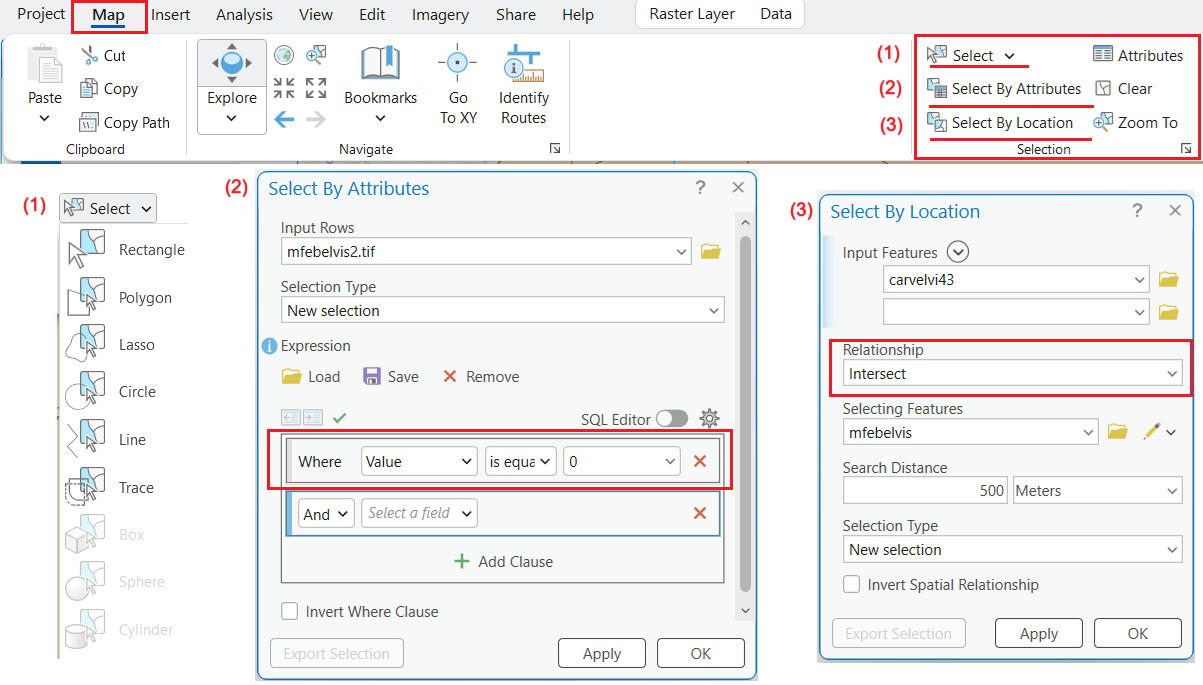
\includegraphics[width=1\textwidth,height=\textheight]{images/conversion_formatos/select_options_pro.png}

}

\caption{Opciones de selección ArcGIS Pro. Los números hacen referencia
a la tabla de herramientas (Tabla~\ref{tbl-herramientas-seleccion}).}

\end{figure}%

\subsubsection{\texorpdfstring{\textbf{QGIS}}{QGIS}}

\begin{figure}[H]

{\centering 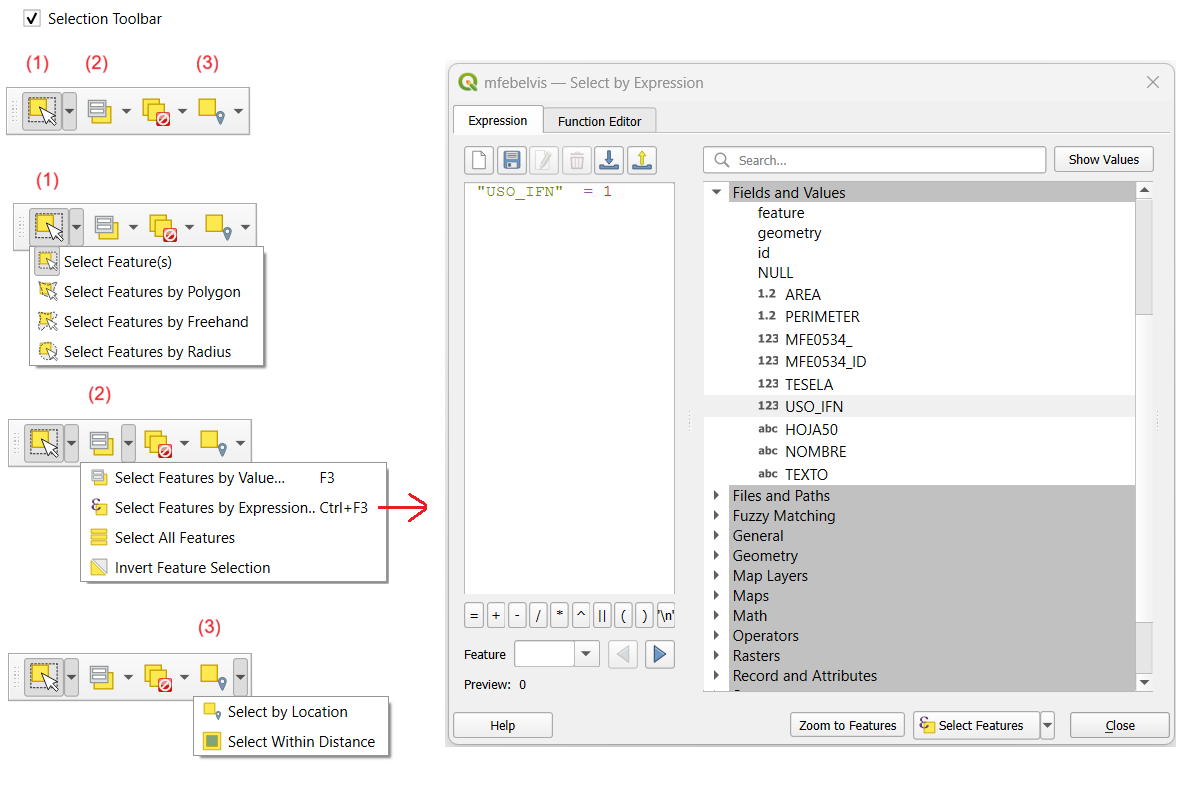
\includegraphics[width=1\textwidth,height=\textheight]{images/conversion_formatos/select_options_qgis.png}

}

\caption{Opciones de selección QGIS - Seleccionar por Expresión. Los
números hacen referencia a la tabla de herramientas
(Tabla~\ref{tbl-herramientas-seleccion})}

\end{figure}%%
\begin{figure}[H]

{\centering 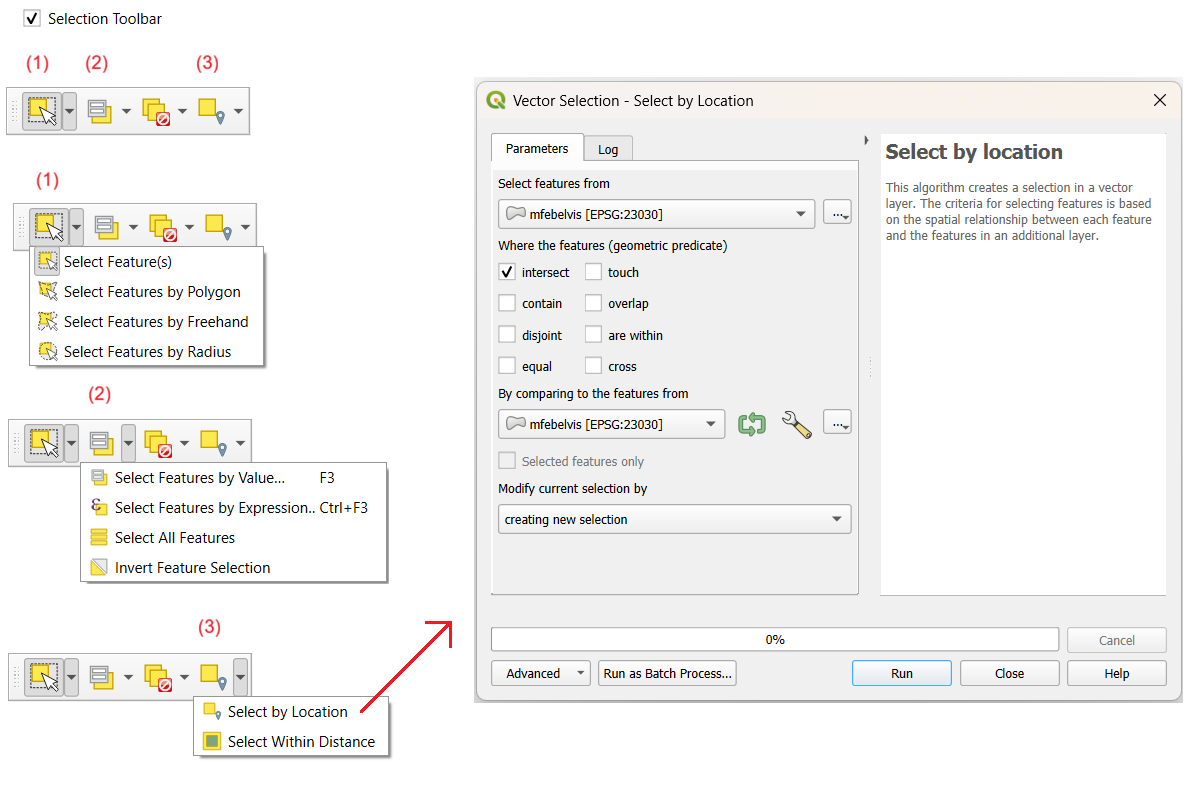
\includegraphics[width=1\textwidth,height=\textheight]{images/conversion_formatos/select_options_qgis2.png}

}

\caption{Opciones de selección QGIS - Seleccionar por Ubicación. Los
números hacen referencia a la tabla de herramientas
(Tabla~\ref{tbl-herramientas-seleccion})}

\end{figure}%

\subsubsection{\texorpdfstring{\textbf{Tabla de Atributos: ArcGIS Pro y
QGIS}}{Tabla de Atributos: ArcGIS Pro y QGIS}}

\begin{figure}[H]

{\centering 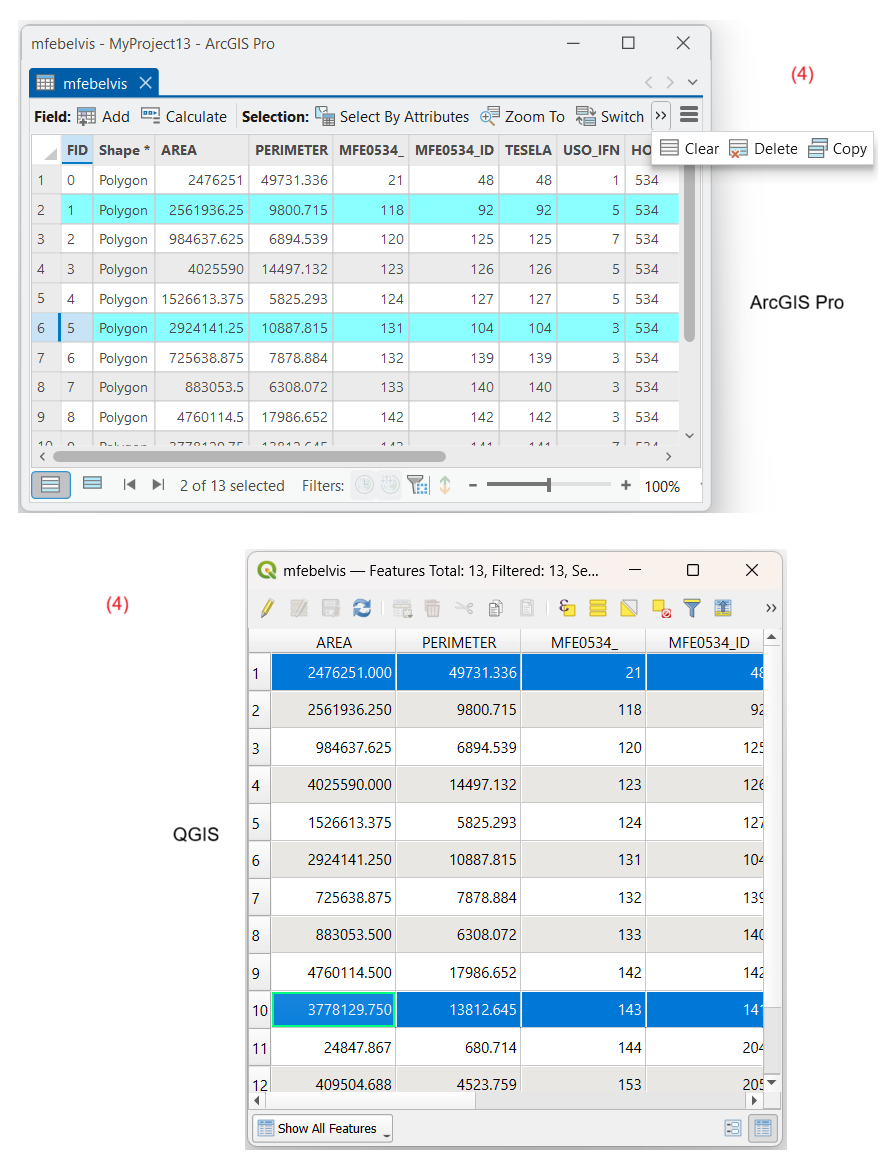
\includegraphics[width=1\textwidth,height=\textheight]{images/conversion_formatos/select_by_table_of_attributes.png}

}

\caption{Selección usando la Tabla de Atributos: ArcGIS Pro (arriba) y
QGIS (abajo). Los números hacen referencia a la tabla de herramientas
(Tabla~\ref{tbl-herramientas-seleccion})}

\end{figure}%

\textbf{Paso 1: Obtención de líneas}

\subsubsection{Flujo en ArcGIS Pro}

\begin{enumerate}
\def\labelenumi{\arabic{enumi}.}
\tightlist
\item
  Abra la herramienta \texttt{Raster\ to\ Polyline} (Ráster a
  polilínea).
\item
  En \texttt{Input\ raster} (Ráster de entrada), elija el tema de
  carreteras \texttt{Carbelvi4}.
\item
  En \texttt{Field} (Campo), asegúrese de seleccionar el campo
  \textbf{\texttt{Value}} (Valor).
\item
  En \texttt{Output\ polyline\ features} (Entidades de polilínea de
  salida), asigne el nombre \texttt{carbelvi43.shp}.
\item
  Mantenga activada la opción \texttt{Simplify\ polylines} (Simplificar
  polilíneas) para generalizar las líneas (equivalente a
  \texttt{Generalize\ lines} en versiones anteriores) y ejecute.
\end{enumerate}

\subsubsection{Flujo en QGIS (vía GRASS)}

\begin{enumerate}
\def\labelenumi{\arabic{enumi}.}
\tightlist
\item
  En la Caja de Herramientas de Procesos, busque \texttt{r.to.vect} (de
  GRASS).
\item
  En \texttt{Input\ raster\ layer} (Capa ráster de entrada), seleccione
  \texttt{Carbelvi4}.
\item
  En \texttt{Feature\ type} (Tipo de entidad), elija \texttt{line}
  (línea).
\item
  En el campo de valores, asegúrese de utilizar la columna que
  representa el \textbf{\texttt{Value}}.
\item
  Active \texttt{Smooth\ corners\ of\ data\ features} (Suavizar
  esquinas) si desea generalizar la geometría.
\item
  Guarde el archivo de salida como \texttt{carbelvi43.shp} y ejecute.
\end{enumerate}

Observe que un nuevo tema de vías vectoriales ha sido creado y
desplegado sobre su mapa base.

\textbf{Paso 2: Obtención de polígonos}

Repita a continuación el proceso para la capa ráster del mapa forestal
de la zona de Belvís (\texttt{mfebelvis2.tif}), solicitando en la
herramienta (\texttt{Raster\ to\ Polygon} en ArcGIS Pro o
\texttt{Polygonize} en QGIS) que el tipo de objeto de salida sea
polígono. Nuevamente, asegúrese de seleccionar el campo
\textbf{\texttt{Value}} para la conversión.

\textbf{Análisis de los resultados de salida:} Abra la tabla de
atributos de la nueva capa vectorial de polígonos generada
(\texttt{mfebelvis23.shp}). Observe que: 1. El valor temático de cada
píxel (el código de uso del suelo) se almacena en una columna
específica, generalmente llamada \texttt{gridcode} o
\texttt{grid\_code}, de cada polígono resultante. 2. Además, cada
polígono nuevo creado tiene un identificador distinto y único (el
\texttt{ID} o \texttt{FID}) que puede servir para vincular cada uno de
ellos con un registro externo de la tabla de atributos.

\subsection{Ejercicio 9: Importar una capa vectorial a una base de datos
PostGIS}\label{ejercicio-9-importar-una-capa-vectorial-a-una-base-de-datos-postgis}

El almacenamiento de datos espaciales en bases de datos relacionales
como PostgreSQL (con su extensión espacial PostGIS) es el estándar
actual. En este ejercicio, nos conectaremos a un contenedor local de
PostGIS.

Aprovecharemos este ejercicio para ilustrar una limitación clásica de
interoperabilidad: intentaremos exportar los datos usando ArcGIS Pro (lo
cual nos arrojará un error por diseño del software) y luego resolveremos
la tarea usando QGIS, que nos permite escribir sin restricciones en
bases de datos nativas.

\begin{itemize}
\tightlist
\item
  \textbf{Objetivo:} Establecer una conexión a PostGIS, comprender las
  restricciones de escritura de los clientes comerciales sobre bases de
  datos crudas, e importar exitosamente el shapefile.
\item
  \textbf{Herramientas:} Conector de bases de datos de ArcGIS Pro (para
  explorar la restricción) y el \textbf{DB Manager} (Administrador de
  BBDD) de QGIS (para la carga exitosa).
\item
  \textbf{Datos de entrada:} Capa poligonal \texttt{mfebelvis.shp}.
\item
  \textbf{Datos de salida:} Tabla espacial \texttt{mfebelvis} almacenada
  dentro de la base de datos PostgreSQL.
\end{itemize}

\textbf{Paso 1: Parámetros de conexión}

Asegúrese de que su contenedor Docker
(\texttt{contenedor\_postgis\_unal}) esté en ejecución. Los parámetros
que utilizaremos son los siguientes:

\begin{itemize}
\tightlist
\item
  \textbf{Host / Servidor:} \texttt{127.0.0.1}
\item
  \textbf{Puerto:} \texttt{5434}
\item
  \textbf{Base de datos:} \texttt{sig\_db\_unal}
\item
  \textbf{Usuario:} \texttt{profe\_unal}
\item
  \textbf{Contraseña:} \texttt{geomatica2025}
\end{itemize}

\textbf{Paso 2: Conexión, el error 000210 y la importación exitosa}

\subsubsection{Flujo en ArcGIS Pro (El Error Educativo)}

\begin{enumerate}
\def\labelenumi{\arabic{enumi}.}
\tightlist
\item
  En el panel \textbf{Catalog} (Catálogo), haga clic derecho en
  \textbf{Databases} (Bases de datos) y seleccione \textbf{New Database
  Connection} (Nueva conexión de base de datos).
\item
  Configure la ventana con los parámetros del Paso 1. Para agregar el
  puerto, en la sección \textbf{Additional Properties} (Propiedades
  adicionales), escriba \texttt{Port} y \texttt{5434}. Haga clic en
  \textbf{OK} (Aceptar).
\end{enumerate}

\begin{figure}[H]

{\centering 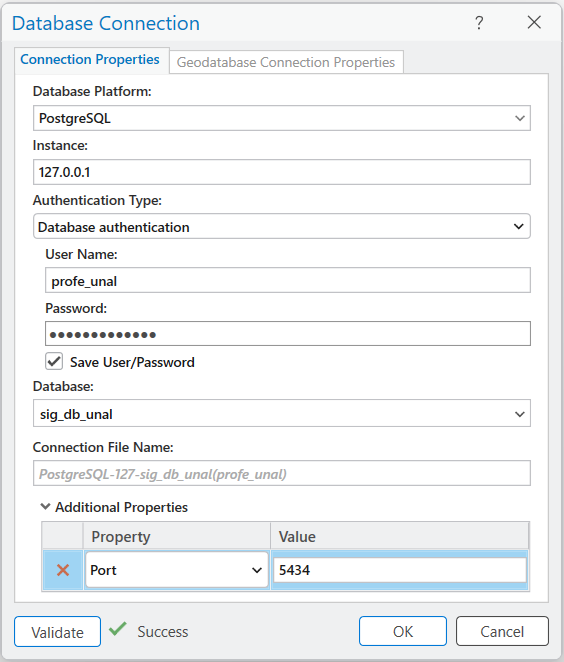
\includegraphics[width=0.55\textwidth,height=\textheight]{images/conversion_formatos/conexion_postgis_pro.png}

}

\caption{Configuración de conexión a PostgreSQL en ArcGIS Pro.}

\end{figure}%

\begin{enumerate}
\def\labelenumi{\arabic{enumi}.}
\setcounter{enumi}{2}
\tightlist
\item
  Haga clic derecho sobre su capa \texttt{mfebelvis} -\textgreater{}
  \textbf{Data} (Datos) -\textgreater{} \textbf{Export Features}
  (Exportar entidades).
\item
  En \textbf{Output Feature Class} (Clase de entidad de salida), navegue
  hasta su conexión. Verá que ArcGIS intenta nombrar la salida como
  \texttt{sig\_db\_unal.profe\_unal.mfebelvis}. Si intenta forzar la
  salida hacia el esquema público
  (\texttt{sig\_db\_unal.public.mfebelvis}) y ejecuta, \textbf{la
  herramienta fallará}.
\end{enumerate}

\begin{figure}[H]

{\centering 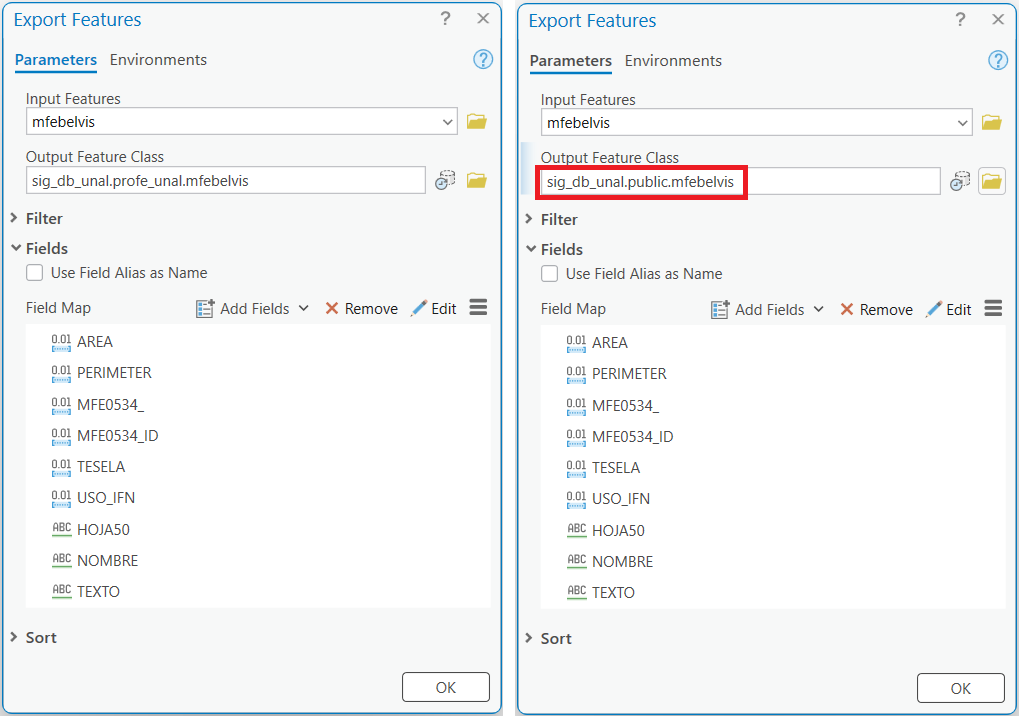
\includegraphics[width=0.85\textwidth,height=\textheight]{images/conversion_formatos/export_features_postgis_pro.png}

}

\caption{Herramienta Export Features. A la izquierda la ruta por
defecto, a la derecha el intento forzando el esquema public.}

\end{figure}%%
\begin{figure}[H]

{\centering 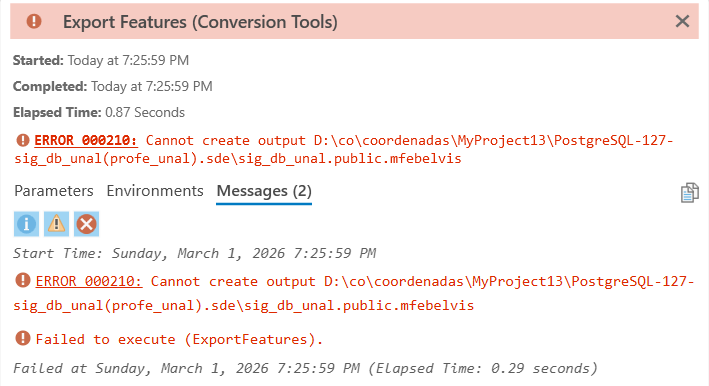
\includegraphics[width=0.7\textwidth,height=\textheight]{images/conversion_formatos/error_no_esquema_profe_unal.png}

}

\caption{ERROR 000210 al intentar exportar la capa desde ArcGIS Pro a
PostgreSQL nativo.}

\end{figure}%

\paragraph{ERROR 000210 al cargar un Shapefile en
PostgreSQL/PostGIS}\label{error-000210-al-cargar-un-shapefile-en-postgresqlpostgis}

\textbf{¿Qué significa el ERROR 000210?}

En ArcGIS Pro, el
\textbf{\texttt{ERROR\ 000210:\ Cannot\ create\ output}} indica que el
sistema no puede crear el dataset de salida. Cuando se trabaja con
PostgreSQL + PostGIS (sin habilitar \emph{Enterprise Geodatabase}), este
error generalmente está relacionado con \textbf{permisos, esquemas y
propiedad}, no con el shapefile en sí.

\textbf{¿Por qué ocurre en una base PostgreSQL/PostGIS nativa?}

En una conexión directa a PostgreSQL:

\begin{itemize}
\tightlist
\item
  ArcGIS Pro intenta crear la tabla en el \textbf{esquema asociado al
  usuario conectado}.
\item
  PostgreSQL, por convención, utiliza un esquema con el mismo nombre del
  usuario.
\item
  El usuario debe:

  \begin{itemize}
  \tightlist
  \item
    Tener un esquema propio.
  \item
    Ser propietario (\emph{owner}) de ese esquema.
  \item
    Tener permisos \texttt{CREATE} y \texttt{USAGE}.
  \end{itemize}
\end{itemize}

Si el esquema no existe o el usuario no es propietario, ArcGIS Pro no
puede crear la tabla y genera el \texttt{ERROR\ 000210}.

\begin{quote}
No se trata exactamente de una ``regla de seguridad de Esri'', sino de
la interacción entre:

\begin{itemize}
\tightlist
\item
  La gestión de esquemas y permisos en PostgreSQL.
\item
  La forma en que ArcGIS Pro resuelve el esquema de escritura.
\end{itemize}
\end{quote}

Además, en muchas instalaciones modernas, el esquema \texttt{public} no
permite la creación de objetos por defecto.

\begin{center}\rule{0.5\linewidth}{0.5pt}\end{center}

\textbf{Posible solución en PostgreSQL}

Si el usuario es \texttt{profe\_unal}, se debería ejecutar el siguiente
bloque desde un cliente SQL:

\begin{Shaded}
\begin{Highlighting}[]
\KeywordTok{CREATE} \KeywordTok{SCHEMA}\NormalTok{ profe\_unal }\KeywordTok{AUTHORIZATION}\NormalTok{ profe\_unal;}
\KeywordTok{GRANT} \KeywordTok{ALL} \KeywordTok{ON} \KeywordTok{SCHEMA}\NormalTok{ profe\_unal }\KeywordTok{TO}\NormalTok{ profe\_unal;}
\KeywordTok{ALTER} \FunctionTok{USER}\NormalTok{ profe\_unal }\KeywordTok{SET}\NormalTok{ search\_path }\KeywordTok{TO}\NormalTok{ profe\_unal, }\KeywordTok{public}\NormalTok{;}
\end{Highlighting}
\end{Shaded}

Esto garantiza que: - El esquema exista. - El usuario sea propietario. -
El \texttt{search\_path} apunte primero a su propio esquema.

\begin{center}\rule{0.5\linewidth}{0.5pt}\end{center}

\textbf{Decisión en este entorno}

Dado que nuestro contenedor es una instalación limpia de PostgreSQL +
PostGIS (sin habilitar \emph{Enterprise Geodatabase}), y el objetivo del
ejercicio no es administrar roles avanzados de bases de datos,
utilizaremos QGIS para cargar los datos directamente en PostGIS y
continuar el flujo de trabajo.

\subsubsection{Flujo en QGIS (La Solución)}

A diferencia de ArcGIS Pro, QGIS es de código abierto y nos permite
interactuar de forma nativa con PostGIS sin exigir la creación de
esquemas ligados al nombre de usuario.

\begin{enumerate}
\def\labelenumi{\arabic{enumi}.}
\tightlist
\item
  En el panel \textbf{Browser} (Navegador), haga clic derecho sobre
  \textbf{PostgreSQL} y seleccione \textbf{New Connection\ldots{}}
  (Conexión nueva\ldots).
\item
  Llene el formulario con los parámetros del Paso 1. En \textbf{Name}
  (Nombre) asigne un alias (ej. \texttt{PostGIS\_UNAL}).
\item
  Haga clic en \textbf{Test Connection} (Probar conexión). Si es
  exitosa, haga clic en \textbf{OK} (Aceptar).
\end{enumerate}

\begin{figure}[H]

{\centering 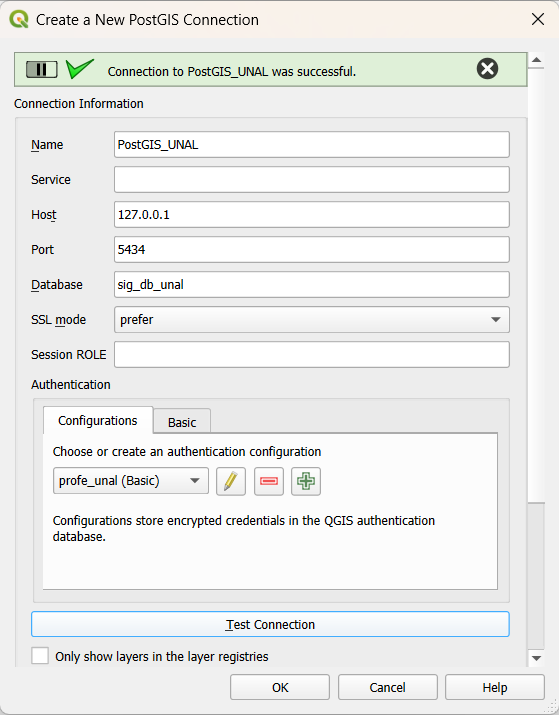
\includegraphics[width=0.6\textwidth,height=\textheight]{images/conversion_formatos/conexion_postgis_qgis.png}

}

\caption{Configuración y prueba de la nueva conexión a PostGIS en QGIS.}

\end{figure}%

\begin{enumerate}
\def\labelenumi{\arabic{enumi}.}
\setcounter{enumi}{3}
\tightlist
\item
  Para importar la capa:

  \begin{itemize}
  \tightlist
  \item
    Vaya al menú superior \textbf{Database} (Base de datos)
    -\textgreater{} \textbf{DB Manager} (Administrador de BBDD).
  \item
    Despliegue el árbol de \emph{PostGIS} -\textgreater{}
    \emph{PostGIS\_UNAL} -\textgreater{} esquema \emph{public}.
  \item
    Haga clic en el botón \textbf{Import Layer/File} (Importar
    Capa/Archivo) en la barra superior (icono de flecha hacia abajo).
  \item
    Seleccione \texttt{mfebelvis} como entrada, asigne el nombre de
    tabla \texttt{mfebelvis}, active la opción \textbf{Create spatial
    index} (Crear índice espacial) y haga clic en \textbf{OK} (Aceptar).
    La importación se realizará sin ningún error de permisos.
  \end{itemize}
\end{enumerate}

\begin{figure}[H]

{\centering 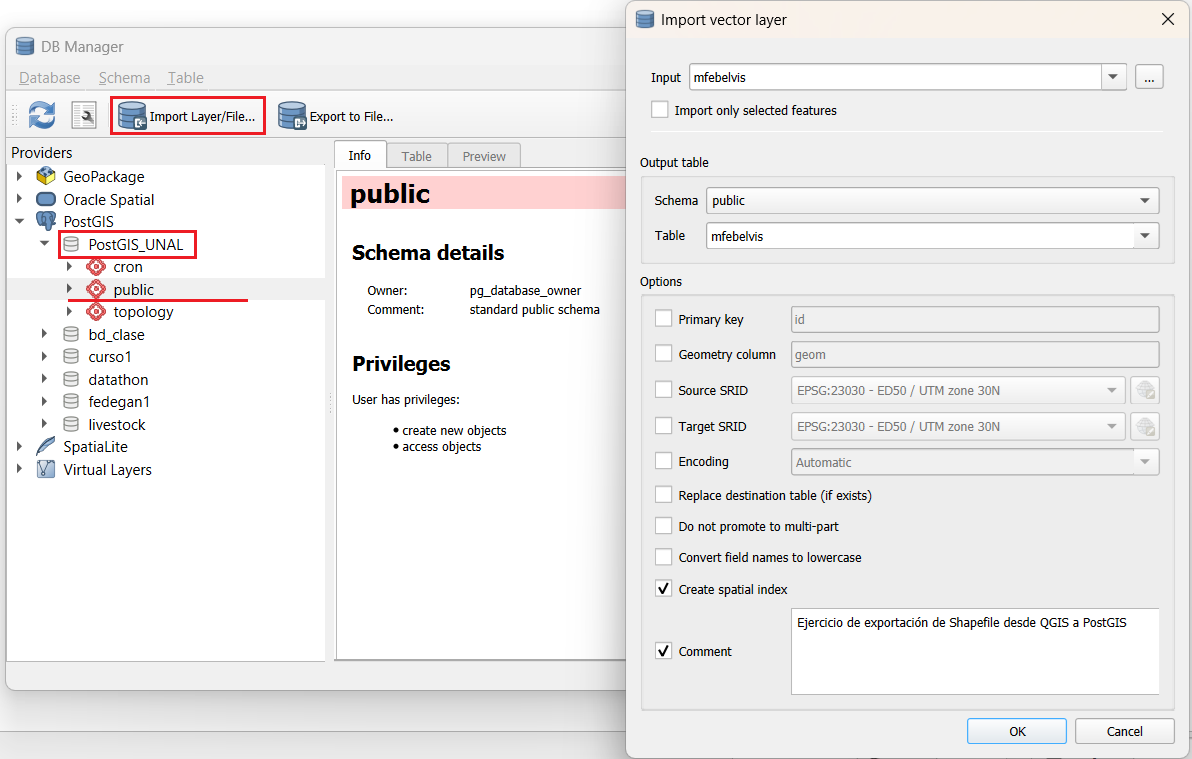
\includegraphics[width=0.75\textwidth,height=\textheight]{images/conversion_formatos/export_shapefile_postgis_qgis.png}

}

\caption{Importación de la capa usando el Administrador de BBDD en
QGIS.}

\end{figure}%%
\begin{figure}[H]

{\centering 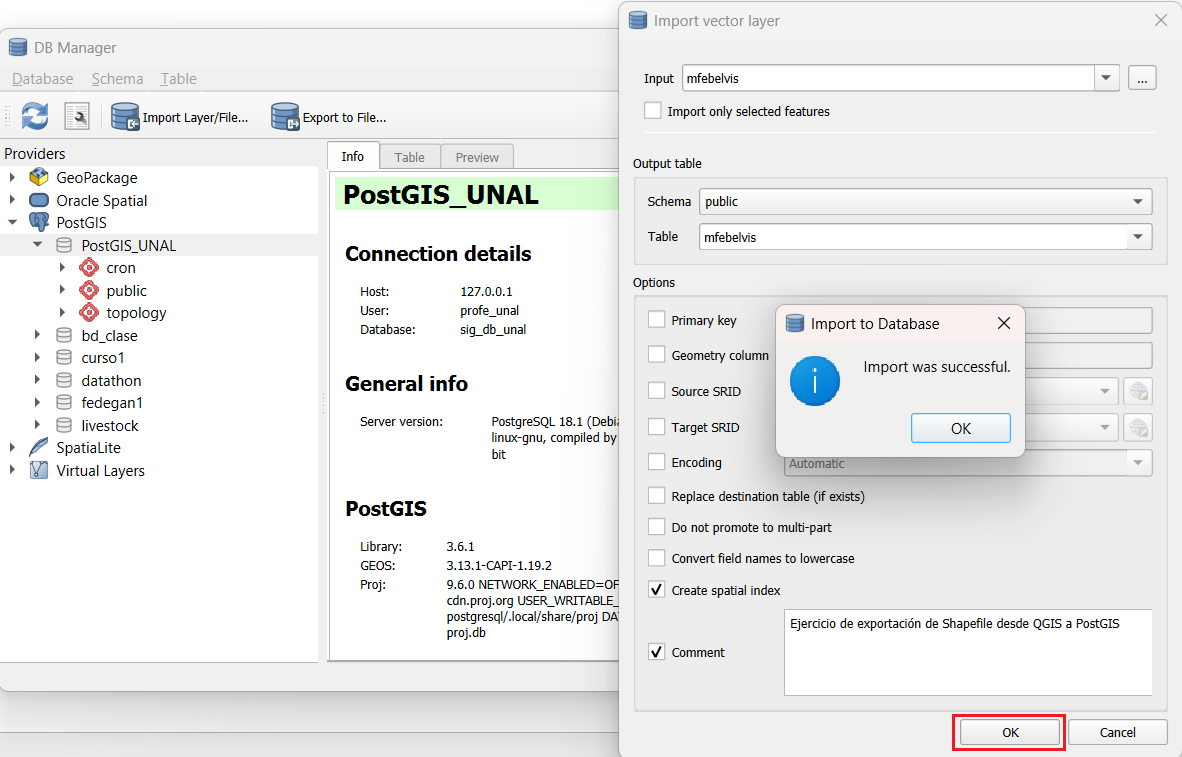
\includegraphics[width=0.75\textwidth,height=\textheight]{images/conversion_formatos/export_shapefile_postgis_qgis_2.png}

}

\caption{Importación de la capa usando el Administrador de BBDD en QGIS.
Salida después de presionar Aceptar.}

\end{figure}%

En esa misma ventana es posible previsualizar el resultado (vectores y
tabla) accediendo a las pestañas correspondientes:

\begin{figure}[H]

{\centering 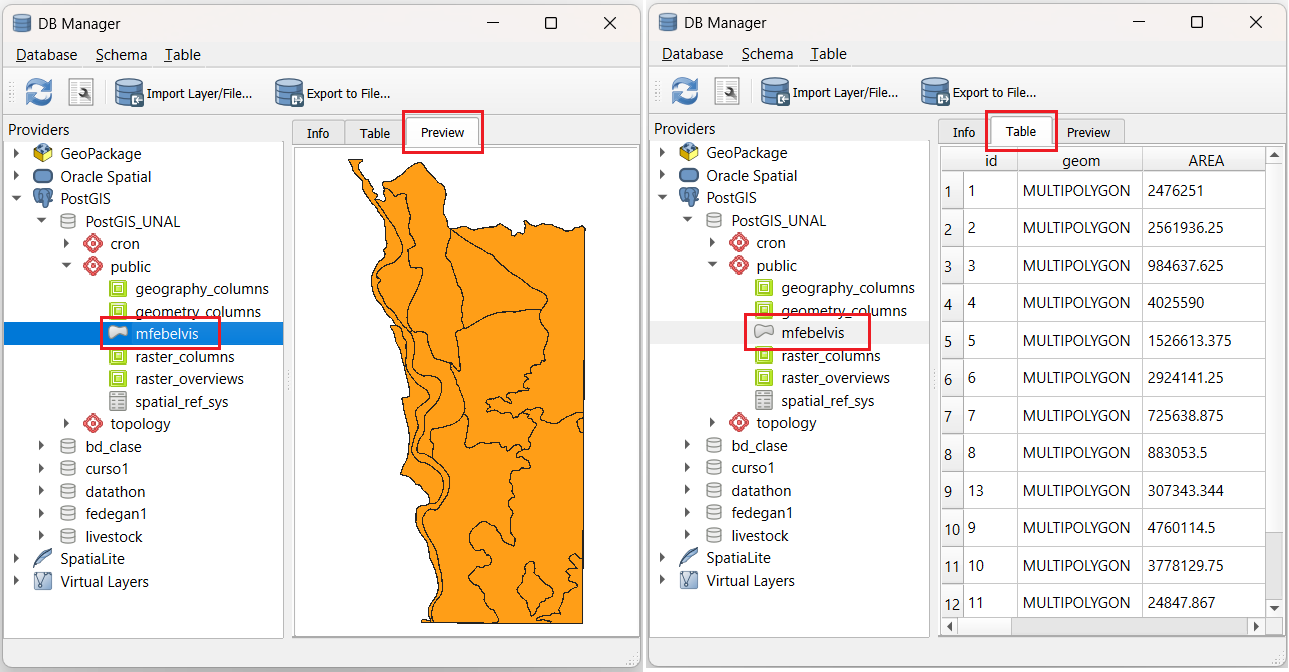
\includegraphics[width=0.75\textwidth,height=\textheight]{images/conversion_formatos/export_shapefile_postgis_qgis_3.png}

}

\caption{Previsualización de vectores y atributos usando el
Administrador de BBDD en QGIS.}

\end{figure}%

\textbf{Paso 3: Verificación e Interoperabilidad}

Apague la capa shapefile original en sus paneles de capas. En QGIS,
arrastre la nueva tabla espacial \texttt{mfebelvis} desde el esquema
\texttt{public} hacia su lienzo de mapa.

\emph{Nota de interoperabilidad:} Aunque ArcGIS Pro no nos permitió
\textbf{escribir} los datos por sus restricciones de esquema, sí nos
permite \textbf{leerlos}. Si regresa a ArcGIS Pro y actualiza su
conexión, verá la tabla recién cargada por QGIS y podrá arrastrarla a su
mapa para su visualización y análisis.

\section{Evaluación Final del
Capítulo}\label{evaluaciuxf3n-final-del-capuxedtulo}

Para poner en práctica los conceptos aprendidos sobre conversión de
formatos e interoperabilidad, deberá resolver los siguientes dos
ejercicios de aplicación técnica.

\subsection{Descarga de Datos}\label{descarga-de-datos}

Puede obtener el paquete de datos necesario para estos ejercicios en el
siguiente enlace:
\href{https://drive.google.com/file/d/1ZhzEN-3Cg7yP-lbsST7zk-mEq4IKvUO4/view?usp=sharing}{👉
Descargar Datos del Taller de Conversión}

\begin{center}\rule{0.5\linewidth}{0.5pt}\end{center}

\subsection{Ejercicio 1: Intercambio de formatos para visualización web
(KML)}\label{ejercicio-1-intercambio-de-formatos-para-visualizaciuxf3n-web-kml}

El formato KML (Keyhole Markup Language) es el estándar de facto para
visualizar datos geográficos en tres dimensiones. Sin embargo, es un
formato rígido: \textbf{Google Earth no realiza proyección al vuelo}; el
archivo debe estar obligatoriamente en coordenadas geográficas
\textbf{WGS84 (EPSG:4326)} para posicionarse correctamente.

\begin{itemize}
\tightlist
\item
  \textbf{Objetivo:} Exportar un dato vectorial a KML asegurando la
  integridad espacial mediante la reproyección previa.
\item
  \textbf{Reto:} Seleccione \textbf{cualquier capa vectorial} de los
  ejercicios anteriores y expórtela a KML siguiendo estos flujos:

  \begin{enumerate}
  \def\labelenumi{\arabic{enumi}.}
  \tightlist
  \item
    \textbf{ArcGIS Pro (Desde el Mapa):} Use la herramienta \textbf{Map
    To KML} (Mapa a KML). Observe cómo se exportan todas las capas
    visibles del lienzo.
  \item
    \textbf{ArcGIS Pro (Desde la Capa):} Use la herramienta
    \textbf{Layer To KML} (Capa a KML). En la pestaña
    \textbf{Environments} (Entornos), verifique que el sistema de salida
    sea \textbf{GCS\_WGS\_1984}.
  \item
    \textbf{QGIS:} Use el menú contextual -\textgreater{}
    \textbf{Export} (Exportar) -\textgreater{} \textbf{Save Features
    As\ldots{}} (Guardar entidades como\ldots). En el cuadro de diálogo,
    cambie el \textbf{CRS} (SRC) a \texttt{EPSG:4326\ -\ WGS\ 84}.
  \end{enumerate}
\item
  \textbf{Validación:} Abra los archivos \texttt{.kmz} resultantes en
  \textbf{Google Earth} y verifique que caigan exactamente sobre la
  superficie terrestre.
\end{itemize}

\begin{center}\rule{0.5\linewidth}{0.5pt}\end{center}

\subsection{Ejercicio 2: ETL Espacial y carga filtrada en
PostGIS}\label{ejercicio-2-etl-espacial-y-carga-filtrada-en-postgis}

Este ejercicio simula un flujo de trabajo profesional donde se deben
aplicar ``reglas de negocio'' (filtros) antes de cargar datos en un
servidor de base de datos.

\begin{itemize}
\tightlist
\item
  \textbf{Datos de entrada:} * Capa vectorial:
  \texttt{MUNICIPIOS\_ISLA\_WGS84.shp} (campo \texttt{NMG} para el
  nombre).

  \begin{itemize}
  \tightlist
  \item
    Filtro espacial: Archivo \texttt{coordenadas.kml} (puntos de
    interés).
  \end{itemize}
\item
  \textbf{Reglas de transformación:}

  \begin{enumerate}
  \def\labelenumi{\arabic{enumi}.}
  \tightlist
  \item
    \textbf{Filtro de Atributo:} No se deben cargar municipios con
    nombres compuestos (ej: ``La Guajira'' se descarta, ``Magdalena'' se
    conserva). \emph{Tip: Busque valores que NO contengan espacios en el
    campo \texttt{NMG}}.
  \item
    \textbf{Filtro Espacial:} Solo se deben cargar los municipios que se
    encuentren dentro de un radio de \textbf{40 km} respecto a los
    puntos del archivo \texttt{coordenadas.kml}.
  \end{enumerate}
\item
  \textbf{Carga Final:} Los datos resultantes que cumplan \textbf{ambas}
  condiciones deben cargarse en el esquema \textbf{\texttt{public}} de
  su base de datos PostGIS local con el nombre de tabla
  \textbf{\texttt{mpios\_kml}}.
\end{itemize}

\begin{center}\rule{0.5\linewidth}{0.5pt}\end{center}

\subsection{Entregables y criterios de
evaluación}\label{entregables-y-criterios-de-evaluaciuxf3n}

El objetivo de esta evaluación es documentar el flujo lógico y demostrar
la capacidad de mover datos entre plataformas de forma segura.

\textbf{1. Archivos de Datos:} * El archivo \texttt{.kmz} generado en el
Ejercicio 1. * Una captura de pantalla de la tabla de atributos en
PostGIS (desde el \textbf{DB Manager} {[}Administrador de BBDD{]} de
QGIS) mostrando los registros finales de la tabla \texttt{mpios\_kml}.

\textbf{2. Documento Analítico (Quarto):} Debe redactar un breve informe
en \textbf{Quarto (\texttt{.qmd})} y renderizarlo en \textbf{HTML o
PDF}. En este documento debe responder:

\begin{itemize}
\tightlist
\item
  \textbf{Sobre el Ejercicio 1 (Sistemas de Coordenadas):} Explique por
  qué es un error intentar abrir un KML con coordenadas planas (metros)
  en Google Earth. ¿Por qué decimos que este visor no tiene ``proyección
  al vuelo''?
\item
  \textbf{Sobre el Ejercicio 2 (Eficiencia ETL):} Para este proceso de
  filtrado, ¿es más eficiente realizar primero el filtro por nombre
  (Atributos) o el filtro por radio de 40 km (Espacial)? Justifique su
  decisión pensando en el ahorro de memoria del computador.
\item
  \textbf{Reflexión sobre Interoperabilidad:} Al cargar los datos en
  PostGIS, vimos que ArcGIS Pro presenta restricciones con el nombre de
  los esquemas. Explique, basado en su experiencia en el Ejercicio 9,
  por qué usar QGIS como ``puente'' facilita la carga de datos hacia
  PostgreSQL/PostGIS.
\end{itemize}

\textbf{3. Repositorio en GitHub:} Suba su carpeta de proyecto (scripts,
archivo \texttt{.qmd} y renders) a un repositorio público en su cuenta
de \textbf{GitHub}.

\begin{itemize}
\tightlist
\item
  \textbf{Entrega:} Envíe únicamente la URL de su repositorio para la
  calificación.
\end{itemize}

\chapter{Introducción a Sensores Remotos y Procesamiento de Imágenes
Satelitales con Google Earth
Engine}\label{introducciuxf3n-a-sensores-remotos-y-procesamiento-de-imuxe1genes-satelitales-con-google-earth-engine}

\section{Requerimientos}\label{requerimientos}

A continuación la lista de software requerido para esta sección:

\begin{itemize}
\tightlist
\item
  ArcGIS Pro (opcional) (\citeproc{ref-price2020arcgis}{Price, 2020}).
  Ver Sección~\ref{sec-arcgis-pro-gee}.
\item
  Caja de herramientas de GEE en ArcGIS Pro (opcional)
  (\citeproc{ref-tanh2025gee}{Tanh, 2025}). Ver
  Sección~\ref{sec-arcgis-pro-gee}
\item
  QGIS instalado con PIXI (\citeproc{ref-wu2025qgisgeedata}{Wu, 2025}).
  Ver Sección~\ref{sec-qgis-gee-pixi}.
\item
  Plugin de GEE en QGIS (\citeproc{ref-wu2025qgisgeedata}{Wu, 2025}).
  Ver Sección~\ref{sec-qgis-gee-pixi}. Ver la
  \href{https://github.com/opengeos/qgis-gee-data-catalogs-plugin}{guía
  de instalación oficial} en inglés.
\item
  Contenedor (Docker) clase de geomática (Python y sus librerías). Ver
  Capítulo~\ref{sec-guia_A}.
\item
  VSCode + Quarto + TinyTex + Extensiones. Ver apéndices de la
  \href{https://github.com/alexyshr/GeomaticaGeneral2026}{guía del
  curso}.
\item
  Registro de usuario GMail para trabajar con GEE. Ver
  \href{https://youtu.be/LoQwc3ne0FU}{video guía de creación y registro
  en GEE} y la sección a continuación.
\item
  Consola Javascript GEE. Ver \href{https://youtu.be/LoQwc3ne0FU}{video
  guía de creación y registro en GEE} y la sección a continuación.
\end{itemize}

\begin{quote}
\textbf{Nota}: En cada sección hay hipervínculos a las guías originales
con todos los detalles (en Inglés). Favor consultar en caso de dudas.
\end{quote}

\section{Registro y Configuración de Google Earth Engine
(GEE)}\label{registro-y-configuraciuxf3n-de-google-earth-engine-gee}

Antes de comenzar, es indispensable contar con una cuenta de
\textbf{Google Cloud} habilitada para \textbf{Google Earth Engine
(GEE)}:

\begin{itemize}
\item
  \textbf{Registro:} Ingresa a \url{https://earthengine.google.com/} y
  regístrate con tu cuenta de GMail o institucional.
\item
  \textbf{Crear un Proyecto:} GEE requiere vincular un proyecto de
  Google Cloud. Crea un nuevo proyecto y configúralo para soportar GEE
  API (ej. \texttt{ee-giswqg}). Mira
  \href{https://console.cloud.google.com/earth-engine/welcome}{esta
  página} para crear un Proyecto de Google cloud y registrarlo con Earth
  Engine.
\item
  \textbf{Habilitar Contributor Tier:} Asegúrate de registrar el
  proyecto bajo la capa gratuita para uso no comercial/educativo
  (\emph{Contributor Tier}).
\end{itemize}

\begin{tcolorbox}[enhanced jigsaw, opacityback=0, left=2mm, colbacktitle=quarto-callout-important-color!10!white, leftrule=.75mm, breakable, titlerule=0mm, rightrule=.15mm, bottomrule=.15mm, arc=.35mm, colback=white, colframe=quarto-callout-important-color-frame, opacitybacktitle=0.6, toptitle=1mm, title=\textcolor{quarto-callout-important-color}{\faExclamation}\hspace{0.5em}{Requisito de Google Cloud}, bottomtitle=1mm, toprule=.15mm, coltitle=black]

Asegúrese de haber creado un proyecto en la consola de Google Cloud y de
tener activadas las \textbf{APIs for Earth Engine} para dicho proyecto;
de lo contrario, el proceso de autenticación fallará.

\href{https://youtu.be/LoQwc3ne0FU}{Video guía de creación y registro en
GEE}

\end{tcolorbox}

\begin{center}\rule{0.5\linewidth}{0.5pt}\end{center}

\section{Entornos de Ejecución para
GEE}\label{entornos-de-ejecuciuxf3n-para-gee}

El código de Google Earth Engine se puede ejecutar desde diferentes
interfaces y lenguajes:

\begin{itemize}
\tightlist
\item
  \textbf{Code Editor:} La plataforma web nativa de Google que utiliza
  \textbf{JavaScript}.
\item
  \textbf{Python:} A través de la API de Python (\texttt{earthengine}).

  \begin{itemize}
  \tightlist
  \item
    En Quarto use la librería \texttt{folium} para crear mapas
    interactivos. \texttt{folium} es menos restrictivo en documentos
    Quarto.
  \item
    En QGIS use la librería \texttt{geemap} para mapas interactivos.
  \item
    En Jupyter Notebooks puede usar \texttt{geemap} o \texttt{folium}.
  \end{itemize}
\item
  \textbf{Desde QGIS:} Utilizando Python mediante el \emph{Google Earth
  Engine Plugin} del profesor Qiusheng Wu.

  \begin{itemize}
  \tightlist
  \item
    La herramienta soporta código Python con \texttt{geemap}.
  \item
    La herramienta convierte código Javascript a código Python.
  \item
    La herramienta permite descargar los datos.
  \end{itemize}
\item
  \textbf{Desde ArcGIS Pro:} A través de Python con el \emph{Add-In}
  oficial de GEE para ArcGIS.

  \begin{itemize}
  \tightlist
  \item
    Este Add-In se basa en el API de Python \texttt{earthengine}.
  \item
    La herramienta permite descargar los datos.
  \end{itemize}
\end{itemize}

\begin{center}\rule{0.5\linewidth}{0.5pt}\end{center}

\subsection{Instalación GEE en QGIS}\label{instalaciuxf3n-gee-en-qgis}

Ver Sección~\ref{sec-qgis-gee-pixi}.

\subsection{Instalación GEE en ArcGIS
Pro}\label{instalaciuxf3n-gee-en-arcgis-pro}

Ver Sección~\ref{sec-arcgis-pro-gee}

\section{Inicialización del Entorno
(Python)}\label{inicializaciuxf3n-del-entorno-python}

Como trabajaremos desde este documento interactivo (QMD), al inicio
debemos autenticar e inicializar nuestra sesión de GEE apuntando a
nuestro proyecto.

\subsection{Python}

\phantomsection\label{python_init}
\begin{Shaded}
\begin{Highlighting}[]
\CommentTok{\# \#| message: false}
\CommentTok{\# \#| warning: false}
\CommentTok{\# \#| echo: false}
\CommentTok{\# \#| eval: false}
\CommentTok{\# \#| results: asis}

\CommentTok{\# 1. IMPORTACIÓN DE LIBRERÍAS}
\CommentTok{\# \textquotesingle{}ee\textquotesingle{} es la librería principal de Google Earth Engine.}
\CommentTok{\# \textquotesingle{}folium\textquotesingle{} nos permite crear mapas interactivos en Python compatibles con Quarto.}
\CommentTok{\# \textquotesingle{}IPython.display\textquotesingle{} se usa para incrustar resultados en el documento final.}
\ImportTok{import}\NormalTok{ ee}

\CommentTok{\# 2. AUTENTICACIÓN}
\CommentTok{\# Este comando abre una ventana en el navegador para dar permisos a Google.}
\CommentTok{\# Solo es necesario correrlo la primera vez o si el token de acceso expira.}
\NormalTok{ee.Authenticate()}

\CommentTok{\# 3. INICIALIZACIÓN DEL PROYECTO}
\CommentTok{\# Debemos especificar el ID del proyecto que creamos en Google Cloud.}
\CommentTok{\# Para este curso usamos el proyecto: "ee{-}giswqg"}
\NormalTok{ee.Initialize(project}\OperatorTok{=}\StringTok{"ee{-}giswqg"}\NormalTok{)}

\BuiltInTok{print}\NormalTok{(}\StringTok{"Google Earth Engine se ha inicializado con éxito!"}\NormalTok{)}
\end{Highlighting}
\end{Shaded}

\begin{verbatim}
Google Earth Engine se ha inicializado con éxito!
\end{verbatim}

\subsection{Javascript}

\phantomsection\label{js_init}%
\begin{Shaded}
\begin{Highlighting}[]
\CommentTok{// 1. INICIALIZACIÓN EN JAVASCRIPT}
\CommentTok{// A diferencia de Python, en el Code Editor de GEE no necesitas importar librerías.}
\CommentTok{// La autenticación es automática siempre que hayas iniciado sesión en tu cuenta.}

\CommentTok{// Solo asegúrate de que en la parte superior derecha de tu Code Editor}
\CommentTok{// esté seleccionado el proyecto: ee{-}giswqg}
\FunctionTok{print}\NormalTok{(}\StringTok{"Google Earth Engine está listo para trabajar en JavaScript."}\NormalTok{)}\OperatorTok{;}
\end{Highlighting}
\end{Shaded}

\subsection{Proceso de Autenticación en Python (Paso a
Paso)}\label{proceso-de-autenticaciuxf3n-en-python-paso-a-paso}

Antes de renderizar el archivo Quarto, ejecuta el chunk de
inicialización de GEE en Python dentro de VSCode. Al ejecutar
\texttt{ee.Authenticate()} por primera vez, deberás otorgar permisos a
la aplicación para que se conecte a tu cuenta de Google Earth Engine.
Sigue estos 6 pasos:

\textbf{Paso 1:} VS Code (o tu entorno) te pedirá abrir un enlace
externo en tu navegador web. Haz clic en \textbf{Open}.

\begin{center}
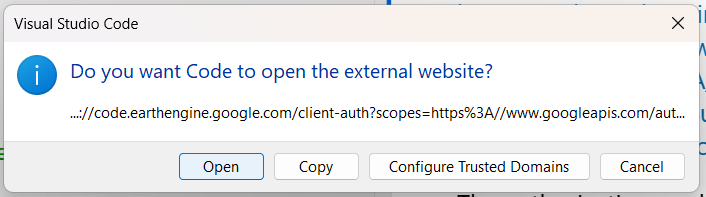
\includegraphics[width=0.7\textwidth,height=\textheight]{images/sensores_remotos/inicializar_gee_1.png}
\end{center}

\begin{center}\rule{0.5\linewidth}{0.5pt}\end{center}

\textbf{Paso 2:} Se abrirá el \emph{Notebook Authenticator} de Earth
Engine. Verifica que estés usando la cuenta correcta y el proyecto
correcto (\texttt{ee-giswqg}). Luego, haz clic en \textbf{GENERATE
TOKEN}.

\begin{center}
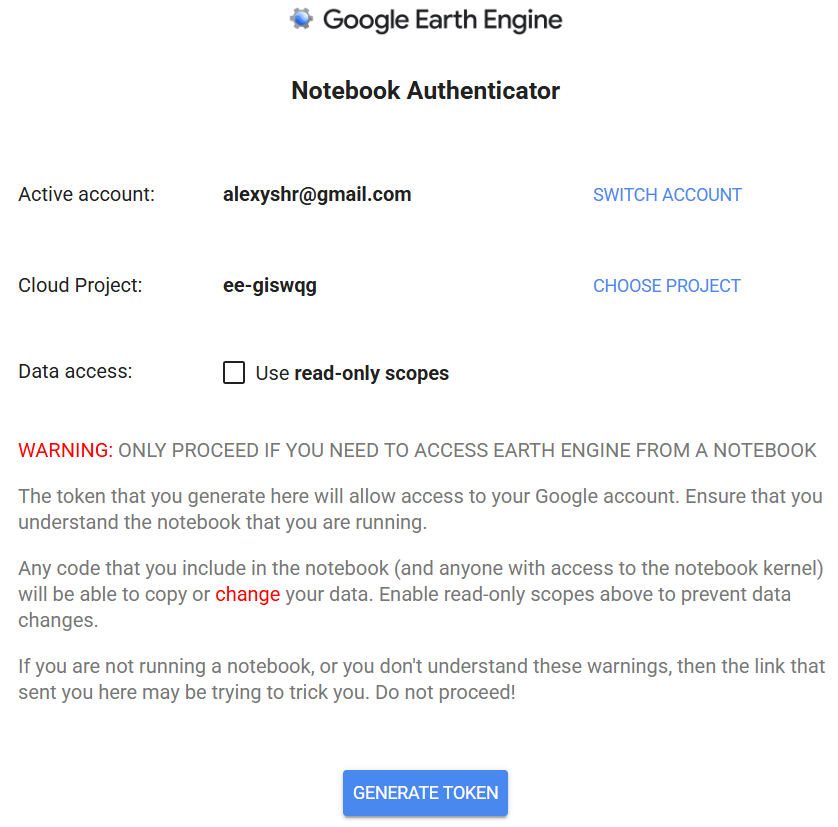
\includegraphics[width=0.7\textwidth,height=\textheight]{images/sensores_remotos/inicializar_gee_2.png}
\end{center}

\begin{center}\rule{0.5\linewidth}{0.5pt}\end{center}

\textbf{Paso 3:} Es probable que Google te muestre una advertencia de
seguridad indicando que la app no está verificada (porque es tu propio
entorno local). Haz clic en \textbf{Continue}.

\begin{center}

\includegraphics[width=0.7\textwidth,height=\textheight]{images/sensores_remotos/inicializar_gee_3.png}
\end{center}

\begin{center}\rule{0.5\linewidth}{0.5pt}\end{center}

\textbf{Paso 4:} Selecciona \textbf{todas} las casillas para otorgar los
permisos necesarios (Drive, Cloud Data, Earth Engine) y haz clic en
\textbf{Continue}.

\begin{center}
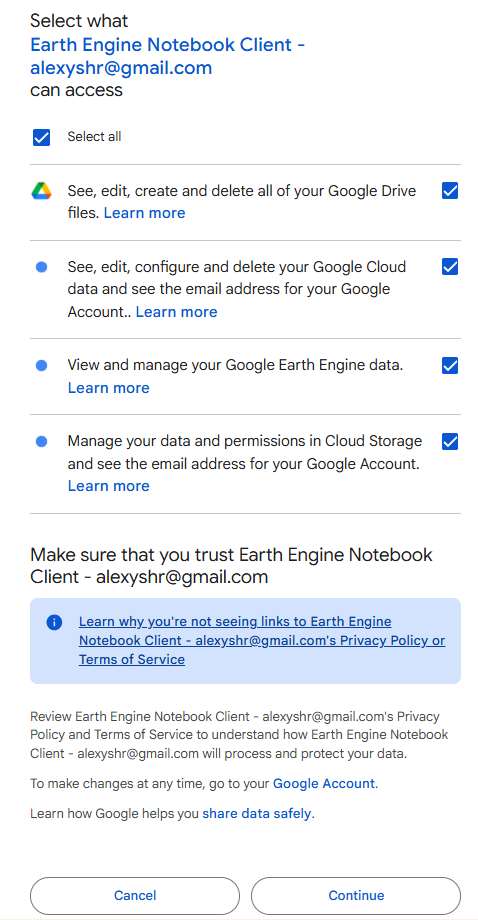
\includegraphics[width=0.6\textwidth,height=\textheight]{images/sensores_remotos/inicializar_gee_4.png}
\end{center}

\begin{center}\rule{0.5\linewidth}{0.5pt}\end{center}

\textbf{Paso 5:} Google generará un código de autorización. Cópialo
usando el botón de la derecha.

\begin{center}
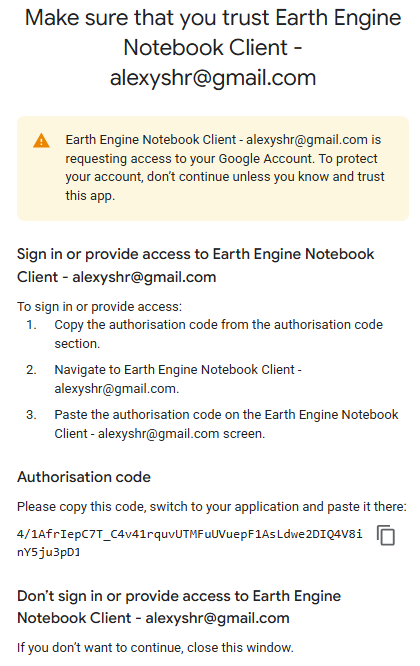
\includegraphics[width=0.6\textwidth,height=\textheight]{images/sensores_remotos/inicializar_gee_5.png}
\end{center}

\begin{center}\rule{0.5\linewidth}{0.5pt}\end{center}

\textbf{Paso 6:} Regresa a VS Code. En la parte superior verás una barra
que dice \emph{Enter verification code}. \textbf{Pega el código allí y
presiona Enter}. ¡Listo, ya estás conectado a las super computadoras de
Google!

\begin{center}
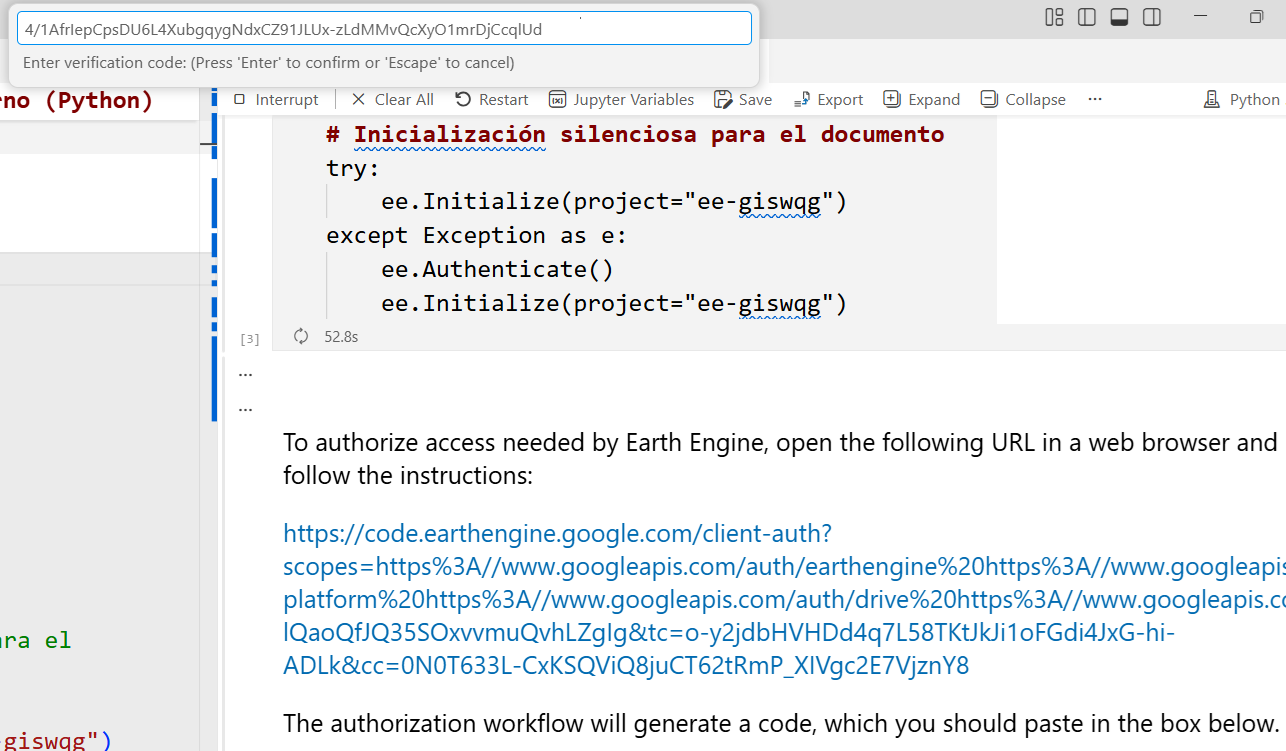
\includegraphics[width=0.85\textwidth,height=\textheight]{images/sensores_remotos/inicializar_gee_6.png}
\end{center}

\begin{center}\rule{0.5\linewidth}{0.5pt}\end{center}

\section{Acceso a los catálogos de
GEE}\label{acceso-a-los-catuxe1logos-de-gee}

Antes de entrar en ejemplos específicos, es vital conocer dónde buscar
la información. Google Earth Engine aloja aproximadamente 120 petabytes
de información espacial lista para el análisis, abarcando más de 40 años
de observaciones históricas y actualizándose diariamente.

Puedes explorar la lista completa, buscar por variables (clima,
elevación, uso del suelo), satélites o etiquetas directamente en su
portal web oficial:

👉
\textbf{\href{https://developers.google.com/earth-engine/datasets/catalog/}{Explorar
el Catálogo de Datos de GEE}}

💡 \textbf{Tip:} \emph{Cada página dentro de este catálogo contiene la
descripción de las bandas, la resolución y, lo más importante, el
fragmento de código exacto
(\texttt{ee.ImageCollection("ID\_DEL\_DATO")}) que necesitas copiar para
llamarlo desde tu script en Python o JavaScript.}

👉 \textbf{\href{https://gee-community-catalog.org/}{Explorar el
Catálogo de la Comunidad de GEE}}. Este catálogo es alimentado y
mantenido por la comunidad y es adicional al catálogo original de datos
de GEE.

\begin{quote}
Los principales tipos de datos dentro de los catálogos son: * Image
Collection (imágenes): Colección de imágenes. * Feature Collection
(datos vectoriales): Colección de vectores.
\end{quote}

\subsection{El catálogo ``tras bambalinas'': Objetos Serializados y
JSON}\label{el-catuxe1logo-tras-bambalinas-objetos-serializados-y-json}

Para entender a un nivel más profundo cómo se comunican nuestras
computadoras con los servidores de Google, es importante saber que el
catálogo web que vemos es solo una ``fachada'' bonita. Detrás de escena,
todo el catálogo de GEE está estructurado usando el estándar
\textbf{STAC} (\emph{SpatioTemporal Asset Catalog}).

En programación, cuando tomamos datos complejos y los convertimos a
texto plano para que viajen por internet sin corromperse, lo llamamos
\textbf{``Objeto Serializado''} (\emph{Serialized Object}). En GEE,
estos objetos serializados viajan en formato \textbf{JSON}
(\emph{JavaScript Object Notation}).

Podemos navegar este catálogo crudo directamente en sus archivos JSON.
Veamos la anatomía de esta estructura de carpetas usando como ejemplo
las imágenes Landsat 9:

\begin{enumerate}
\def\labelenumi{\arabic{enumi}.}
\item
  \textbf{El Catálogo Principal:} Todo empieza en un gran archivo
  ``índice'' que lista todos los proveedores de datos:
  \href{https://earthengine-stac.storage.googleapis.com/catalog/catalog.json}{\texttt{https://earthengine-stac.storage.googleapis.com/catalog/catalog.json}}
\item
  \textbf{La Familia de Satélites (Landsat):} Si dentro de ese índice
  buscamos ``LANDSAT'', el archivo nos redirige a la carpeta específica
  de este programa espacial:
  \href{https://storage.googleapis.com/earthengine-stac/catalog/LANDSAT/catalog.json}{\texttt{https://storage.googleapis.com/earthengine-stac/catalog/LANDSAT/catalog.json}}
\item
  \textbf{El Insumo Específico (Asset ID):} Finalmente, podemos buscar
  nuestro grupo de imágenes Landsat a partir del \emph{Asset ID}:
  \texttt{LANDSAT/LC09/C02/T1\_TOA} (el cual exploraremos a fondo en la
  Sección~\ref{sec-catalogo_landsat8_9}).

  \begin{itemize}
  \tightlist
  \item
    Para buscar dentro del archivo JSON use (\texttt{\_}) en lugar de
    (\texttt{/}), es decir \texttt{LANDSAT\_LC09\_C02\_T1\_TOA}. Con esa
    búsqueda el sistema nos lleva al archivo maestro de metadatos de
    Landsat:
    \href{https://storage.googleapis.com/earthengine-stac/catalog/LANDSAT/LANDSAT_LC09_C02_T1_TOA.json}{\texttt{https://storage.googleapis.com/earthengine-stac/catalog/LANDSAT/LANDSAT\_LC09\_C02\_T1\_TOA.json}}
  \end{itemize}
\end{enumerate}

\begin{quote}
Para buscar dentro del catálogo GEE use el \emph{Asset ID} original:
\texttt{LANDSAT/LC09/C02/T1\_TOA}.
\end{quote}

\textbf{¿Para qué sirve entender esto?}

En el
\href{https://developers.google.com/earth-engine/datasets/catalog/}{catálogo
de GEE} busca \texttt{LANDSAT/LC09/C02/T1\_TOA}. ¡Porque la página web
del catálogo de GEE que consultas a diario simplemente lee este último
archivo JSON (\emph{objetos serializados}) y lo ``maquilla''!

\begin{itemize}
\tightlist
\item
  El texto que aparece en la pestaña \textbf{``Description''} de la
  página web se extrae del campo \texttt{description} del JSON.
\item
  La tabla que ves en la pestaña \textbf{``Bands''} se construye leyendo
  el arreglo \texttt{eo:bands} del JSON.
\item
  Los parámetros y filtros que usas en QGIS o ArcGIS Pro salen
  exactamente de la información contenida en este archivo serializado
  (visible en la pestaña \textbf{``Image Properties''}).
\end{itemize}

Entender que todo en GEE son \emph{objetos serializados} te ayudará más
adelante a comprender por qué tu computadora no colapsa procesando miles
de imágenes: tu máquina solo envía y recibe pequeños archivos de texto
JSON con instrucciones, mientras que la nube hace el trabajo pesado.

\begin{center}\rule{0.5\linewidth}{0.5pt}\end{center}

\section{Catálogo de datos: Landsat 8/9}\label{sec-catalogo_landsat8_9}

En esta sección exploraremos el campus de la Universidad Nacional de
Colombia (Sede Bogotá) utilizando imágenes del satélite Landsat 9.
Landsat es fundamental para entender cambios históricos en la cobertura
terrestre.

\subsection{Entendiendo la colección y el
código}\label{entendiendo-la-colecciuxf3n-y-el-cuxf3digo}

En el catálogo de GEE, la base de datos exacta que vamos a utilizar
tiene el \emph{Asset ID}: \texttt{LANDSAT/LC09/C02/T1\_TOA}. ¿Qué
significa este código tan largo? En Earth Engine, cada parte del nombre
nos da metadatos vitales sobre el insumo:

\begin{itemize}
\tightlist
\item
  \textbf{\texttt{LANDSAT/LC09}}: Indica el programa espacial y el
  satélite específico (Landsat 9).
\item
  \textbf{\texttt{C02} (Collection 2)}: Es la versión más reciente y
  pulida del procesamiento de la NASA/USGS, con mejoras en la precisión
  geográfica y radiométrica.
\item
  \textbf{\texttt{T1} (Tier 1)}: Son los datos de la más alta calidad.
  Han pasado los controles más estrictos de nubosidad y geometría,
  siendo los únicos recomendados para análisis temporales rigurosos.
\item
  \textbf{\texttt{TOA} (Top of Atmosphere)}: Reflectancia al Tope de la
  Atmósfera. Mide la energía de la luz tal cual choca contra el lente
  del satélite en el espacio, sin aplicar correcciones por los gases o
  aerosoles de la atmósfera terrestre.
\end{itemize}

Para procesar estos datos y verlos en pantalla, combinaremos los
servidores de Google con librerías de mapeo en Python. Antes de ver el
código, familiarízate con las herramientas (clases y funciones)
principales que usaremos:

\textbf{El ``Diccionario'' de nuestro Script:}

\begin{longtable}[]{@{}
  >{\raggedright\arraybackslash}p{(\columnwidth - 4\tabcolsep) * \real{0.3000}}
  >{\raggedright\arraybackslash}p{(\columnwidth - 4\tabcolsep) * \real{0.2000}}
  >{\raggedright\arraybackslash}p{(\columnwidth - 4\tabcolsep) * \real{0.5000}}@{}}
\toprule\noalign{}
\begin{minipage}[b]{\linewidth}\raggedright
Función / Clase
\end{minipage} & \begin{minipage}[b]{\linewidth}\raggedright
Librería
\end{minipage} & \begin{minipage}[b]{\linewidth}\raggedright
¿Para qué sirve en nuestro análisis?
\end{minipage} \\
\midrule\noalign{}
\endhead
\bottomrule\noalign{}
\endlastfoot
\texttt{ee.Geometry.Point()} & Earth Engine (\texttt{ee}) & Dibuja una
coordenada matemática exacta \texttt{{[}Longitud,\ Latitud{]}} en los
servidores de Google para indicarle dónde queremos buscar la
información. \\
\texttt{ee.ImageCollection()} & Earth Engine (\texttt{ee}) & Llama a un
``archivo'' gigante que contiene millones de imágenes históricas. A esta
colección le aplicaremos filtros para extraer una sola imagen. \\
\texttt{geemap.Map()} & Geemap & Crea un lienzo o mapa interactivo
especializado en GEE. Es la herramienta estándar para visualizar los
resultados si trabajas desde \textbf{QGIS, VS Code o Jupyter
Notebooks}. \\
\texttt{folium.Map()} & Folium & Crea un mapa interactivo web nativo. Lo
usamos ``tras bambalinas'' en este documento \textbf{Quarto} porque es
ultra-liviano, no usa widgets pesados y evita que la presentación
colapse. \\
\texttt{folium.TileLayer()} & Folium & Permite inyectar los ``Tiles''
(cuadritos de imagen renderizados por los servidores de Google)
directamente sobre nuestro mapa web. \\
\texttt{folium.LayerControl()} & Folium & Añade el clásico menú en la
esquina superior del mapa que le permite al usuario encender y apagar
las capas satelitales a su gusto. \\
\end{longtable}

Finalmente, al momento de visualizar la imagen, usaremos los canales de
luz (bandas) específicos del sensor de Landsat 9:

\begin{longtable}[]{@{}
  >{\raggedright\arraybackslash}p{(\columnwidth - 4\tabcolsep) * \real{0.1667}}
  >{\raggedright\arraybackslash}p{(\columnwidth - 4\tabcolsep) * \real{0.1667}}
  >{\raggedright\arraybackslash}p{(\columnwidth - 4\tabcolsep) * \real{0.6667}}@{}}
\toprule\noalign{}
\begin{minipage}[b]{\linewidth}\raggedright
Banda
\end{minipage} & \begin{minipage}[b]{\linewidth}\raggedright
Resolución
\end{minipage} & \begin{minipage}[b]{\linewidth}\raggedright
Descripción
\end{minipage} \\
\midrule\noalign{}
\endhead
\bottomrule\noalign{}
\endlastfoot
\textbf{B2, B3, B4} & 30m & Espectro Visible (Azul, Verde, Rojo). Forman
el ``Color Verdadero''. \\
\textbf{B5} & 30m & Infrarrojo Cercano (NIR). Luz invisible al ojo
humano, pero vital para analizar el vigor y salud de la vegetación. \\
\end{longtable}

\begin{tcolorbox}[enhanced jigsaw, opacityback=0, left=2mm, colbacktitle=quarto-callout-note-color!10!white, leftrule=.75mm, breakable, titlerule=0mm, rightrule=.15mm, bottomrule=.15mm, arc=.35mm, colback=white, colframe=quarto-callout-note-color-frame, opacitybacktitle=0.6, toptitle=1mm, title={🧠 Concepto Clave: Cliente vs.~Servidor (\texttt{.getInfo()})}, bottomtitle=1mm, toprule=.15mm, coltitle=black]

En los siguientes códigos de Python verás que usamos repetidamente la
función \texttt{.getInfo()}. Como vimos hace un momento, GEE funciona
enviando instrucciones desde tu computadora (el \textbf{Cliente}) a las
super-computadoras de Google (el \textbf{Servidor}). Las imágenes
pesadas se procesan y se quedan allá para no colapsar tu PC.

Sin embargo, cuando necesitas leer un resultado concreto (como una fecha
o el porcentaje de nubes) en tu pantalla de VS Code o QGIS, usas
\texttt{.getInfo()}. Este comando le dice a Google: \emph{``Por favor,
empaqueta este dato específico, procésalo y envíame el resultado de
regreso a mi computadora (como un diccionario de Python o un JSON)''}.
¡Es tu puente de retorno desde la nube!

\end{tcolorbox}

\subsection{Python}

\begin{Shaded}
\begin{Highlighting}[]
\CommentTok{\# \#| eval: false}

\CommentTok{\# Código usando Folium!}

\ImportTok{import}\NormalTok{ ee}
\ImportTok{import}\NormalTok{ folium}
\ImportTok{import}\NormalTok{ datetime }\CommentTok{\# Para manejar tiempos y fechas}
\ImportTok{import}\NormalTok{ json }\CommentTok{\# Librería nativa de Python para manejar JSON}

\CommentTok{\# 1. DEFINICIÓN DEL PUNTO GEOGRÁFICO}
\CommentTok{\# REGLA DE ORO EN GEE: El orden de las coordenadas es siempre [LONGITUD, LATITUD].}
\NormalTok{unal\_punto }\OperatorTok{=}\NormalTok{ ee.Geometry.Point([}\OperatorTok{{-}}\FloatTok{74.084}\NormalTok{, }\FloatTok{4.638}\NormalTok{])}

\CommentTok{\# 2. EXPLORAR TODAS LAS OPCIONES Y FILTRAR (Proceso en Servidor)}
\CommentTok{\# Filtramos la colección Landsat 9 para el año 2023 sobre la UNAL Bogotá.}
\NormalTok{coleccion\_l9 }\OperatorTok{=}\NormalTok{ (ee.ImageCollection(}\StringTok{"LANDSAT/LC09/C02/T1\_TOA"}\NormalTok{) }
\NormalTok{    .filterBounds(unal\_punto) }
\NormalTok{    .filterDate(}\StringTok{\textquotesingle{}2023{-}01{-}01\textquotesingle{}}\NormalTok{, }\StringTok{\textquotesingle{}2023{-}12{-}31\textquotesingle{}}\NormalTok{) }
\NormalTok{    .sort(}\StringTok{\textquotesingle{}CLOUD\_COVER\textquotesingle{}}\NormalTok{))}

\CommentTok{\# 3. DIAGNÓSTICO: EXTRAER EL TOP 3 DE IMÁGENES}
\NormalTok{ids }\OperatorTok{=}\NormalTok{ coleccion\_l9.aggregate\_array(}\StringTok{\textquotesingle{}system:id\textquotesingle{}}\NormalTok{).getInfo()}
\NormalTok{nubes }\OperatorTok{=}\NormalTok{ coleccion\_l9.aggregate\_array(}\StringTok{\textquotesingle{}CLOUD\_COVER\textquotesingle{}}\NormalTok{).getInfo()}
\NormalTok{fechas }\OperatorTok{=}\NormalTok{ coleccion\_l9.aggregate\_array(}\StringTok{\textquotesingle{}system:time\_start\textquotesingle{}}\NormalTok{).getInfo()}

\BuiltInTok{print}\NormalTok{(}\StringTok{"{-}{-}{-} TOP 3 IMÁGENES CON MENOS NUBES EN EL AÑO 2023 (TODA LA ESCENA) {-}{-}{-}"}\NormalTok{)}
\ControlFlowTok{for}\NormalTok{ i }\KeywordTok{in} \BuiltInTok{range}\NormalTok{(}\BuiltInTok{min}\NormalTok{(}\DecValTok{3}\NormalTok{, }\BuiltInTok{len}\NormalTok{(ids))):}
    \CommentTok{\# ACTUALIZACIÓN: Usamos fromtimestamp con datetime.UTC para evitar el DeprecationWarning}
\NormalTok{    fecha\_legible }\OperatorTok{=}\NormalTok{ datetime.datetime.fromtimestamp(fechas[i] }\OperatorTok{/} \FloatTok{1000.0}\NormalTok{, datetime.UTC).strftime(}\StringTok{\textquotesingle{}\%Y{-}\%m{-}}\SpecialCharTok{\%d}\StringTok{\textquotesingle{}}\NormalTok{)}
    \BuiltInTok{print}\NormalTok{(}\SpecialStringTok{f"Opción }\SpecialCharTok{\{}\NormalTok{i}\OperatorTok{+}\DecValTok{1}\SpecialCharTok{\}}\SpecialStringTok{ | Nubes: }\SpecialCharTok{\{}\NormalTok{nubes[i]}\SpecialCharTok{:.2f\}}\SpecialStringTok{\% | Fecha: }\SpecialCharTok{\{}\NormalTok{fecha\_legible}\SpecialCharTok{\}}\SpecialStringTok{"}\NormalTok{)}
    \BuiltInTok{print}\NormalTok{(}\SpecialStringTok{f"ID: }\SpecialCharTok{\{}\NormalTok{ids[i]}\SpecialCharTok{\}}\CharTok{\textbackslash{}n}\SpecialStringTok{"}\NormalTok{)}
\BuiltInTok{print}\NormalTok{(}\StringTok{"{-}{-}{-}{-}{-}{-}{-}{-}{-}{-}{-}{-}{-}{-}{-}{-}{-}{-}{-}{-}{-}{-}{-}{-}{-}{-}{-}{-}{-}{-}{-}{-}{-}{-}{-}{-}{-}{-}{-}{-}{-}{-}{-}{-}{-}{-}{-}{-}{-}{-}{-}{-}{-}{-}{-}{-}{-}{-}{-}{-}{-}{-}{-}{-}"}\NormalTok{)}

\CommentTok{\# 4. SELECCIÓN DEFINITIVA DE LA IMAGEN}
\NormalTok{l9 }\OperatorTok{=}\NormalTok{ coleccion\_l9.first()}

\CommentTok{\# 5. EXPORTAR LOS ARCHIVOS JSON (METADATOS Y SERIALIZADO)}
\NormalTok{id\_exacto }\OperatorTok{=}\NormalTok{ l9.get(}\StringTok{\textquotesingle{}system:id\textquotesingle{}}\NormalTok{).getInfo()}
\BuiltInTok{print}\NormalTok{(}\SpecialStringTok{f"}\CharTok{\textbackslash{}n}\SpecialStringTok{ID de la imagen Landsat 9 seleccionada: }\SpecialCharTok{\{}\NormalTok{id\_exacto}\SpecialCharTok{\}}\SpecialStringTok{"}\NormalTok{)}

\CommentTok{\# A) Exportar Metadatos (Referencia humana)}
\CommentTok{\# Contiene el resultado final: propiedades, fecha, \% de nubes, bandas, etc.}
\NormalTok{metadatos\_json }\OperatorTok{=}\NormalTok{ l9.getInfo()}
\ControlFlowTok{with} \BuiltInTok{open}\NormalTok{(}\StringTok{\textquotesingle{}metadatos\_landsat9.json\textquotesingle{}}\NormalTok{, }\StringTok{\textquotesingle{}w\textquotesingle{}}\NormalTok{) }\ImportTok{as}\NormalTok{ archivo:}
\NormalTok{    json.dump(metadatos\_json, archivo, indent}\OperatorTok{=}\DecValTok{4}\NormalTok{)}
\BuiltInTok{print}\NormalTok{(}\StringTok{"¡Archivo \textquotesingle{}metadatos\_landsat9.json\textquotesingle{} generado! (Explora sus propiedades)"}\NormalTok{)}

\CommentTok{\# B) Exportar Grafo Serializado (Para ArcGIS Pro)}
\CommentTok{\# Contiene las instrucciones puras. Usamos el ID limpio para no confundir a ArcGIS.}
\NormalTok{l9\_limpia }\OperatorTok{=}\NormalTok{ ee.Image(id\_exacto)}
\NormalTok{texto\_json\_serializado }\OperatorTok{=}\NormalTok{ l9\_limpia.serialize()}

\CommentTok{\# TRUCO PARA ARCGIS PRO: Guardamos el resultado empacado directamente como un String.}
\ControlFlowTok{with} \BuiltInTok{open}\NormalTok{(}\StringTok{\textquotesingle{}landsat9\_serializado.json\textquotesingle{}}\NormalTok{, }\StringTok{\textquotesingle{}w\textquotesingle{}}\NormalTok{) }\ImportTok{as}\NormalTok{ archivo:}
\NormalTok{    json.dump(texto\_json\_serializado, archivo)}
\BuiltInTok{print}\NormalTok{(}\StringTok{"¡Archivo \textquotesingle{}landsat9\_serializado.json\textquotesingle{} generado! (Úsalo en la herramienta de ArcGIS Pro)"}\NormalTok{)}


\CommentTok{\# 6. PARÁMETROS DE VISUALIZACIÓN (Composición RGB)}
\NormalTok{vis\_params }\OperatorTok{=}\NormalTok{ \{}\StringTok{\textquotesingle{}bands\textquotesingle{}}\NormalTok{: [}\StringTok{\textquotesingle{}B4\textquotesingle{}}\NormalTok{, }\StringTok{\textquotesingle{}B3\textquotesingle{}}\NormalTok{, }\StringTok{\textquotesingle{}B2\textquotesingle{}}\NormalTok{], }\StringTok{\textquotesingle{}min\textquotesingle{}}\NormalTok{: }\FloatTok{0.0}\NormalTok{, }\StringTok{\textquotesingle{}max\textquotesingle{}}\NormalTok{: }\FloatTok{0.3}\NormalTok{\}}

\CommentTok{\# 7. OBTENER URL DE LOS TILES DE GOOGLE}
\NormalTok{map\_id\_dict }\OperatorTok{=}\NormalTok{ ee.Image(l9).getMapId(vis\_params)}

\CommentTok{\# 8. MENSAJE FINAL CON LOS DETALLES DE LA IMAGEN DESPLEGADA}
\NormalTok{fecha\_capa\_ms }\OperatorTok{=}\NormalTok{ l9.get(}\StringTok{\textquotesingle{}system:time\_start\textquotesingle{}}\NormalTok{).getInfo()}
\CommentTok{\# ACTUALIZACIÓN: Aquí también aplicamos el estándar moderno de Python para UTC}
\NormalTok{fecha\_capa }\OperatorTok{=}\NormalTok{ datetime.datetime.fromtimestamp(fecha\_capa\_ms }\OperatorTok{/} \FloatTok{1000.0}\NormalTok{, datetime.UTC).strftime(}\StringTok{\textquotesingle{}\%Y{-}\%m{-}}\SpecialCharTok{\%d}\StringTok{\textquotesingle{}}\NormalTok{)}
\NormalTok{id\_desplegada }\OperatorTok{=}\NormalTok{ l9.get(}\StringTok{\textquotesingle{}system:id\textquotesingle{}}\NormalTok{).getInfo()}
\NormalTok{nubes\_desplegada }\OperatorTok{=}\NormalTok{ l9.get(}\StringTok{\textquotesingle{}CLOUD\_COVER\textquotesingle{}}\NormalTok{).getInfo()}

\BuiltInTok{print}\NormalTok{(}\StringTok{"}\CharTok{\textbackslash{}n}\StringTok{✅ MAPA GENERADO CON ÉXITO"}\NormalTok{)}
\BuiltInTok{print}\NormalTok{(}\SpecialStringTok{f"Capa desplegada : Landsat 9 RGB {-} }\SpecialCharTok{\{}\NormalTok{fecha\_capa}\SpecialCharTok{\}}\SpecialStringTok{"}\NormalTok{)}
\BuiltInTok{print}\NormalTok{(}\SpecialStringTok{f"ID del archivo  : }\SpecialCharTok{\{}\NormalTok{id\_desplegada}\SpecialCharTok{\}}\SpecialStringTok{"}\NormalTok{)}
\BuiltInTok{print}\NormalTok{(}\SpecialStringTok{f"Nubosidad total : }\SpecialCharTok{\{}\NormalTok{nubes\_desplegada}\SpecialCharTok{:.2f\}}\SpecialStringTok{\%"}\NormalTok{)}
\BuiltInTok{print}\NormalTok{(}\StringTok{"{-}{-}{-}{-}{-}{-}{-}{-}{-}{-}{-}{-}{-}{-}{-}{-}{-}{-}{-}{-}{-}{-}{-}{-}{-}{-}{-}{-}{-}{-}{-}{-}{-}{-}{-}{-}{-}{-}{-}{-}{-}{-}{-}{-}{-}{-}{-}{-}{-}{-}{-}{-}{-}{-}{-}{-}{-}{-}{-}{-}{-}{-}{-}{-}"}\NormalTok{)}

\CommentTok{\# 9. CONFIGURACIÓN DEL MAPA BASE (Folium)}
\CommentTok{\# ¡ATENCIÓN!: Folium usa el orden [LATITUD, LONGITUD].}
\NormalTok{Map\_l9 }\OperatorTok{=}\NormalTok{ folium.Map(location}\OperatorTok{=}\NormalTok{[}\FloatTok{4.638}\NormalTok{, }\OperatorTok{{-}}\FloatTok{74.084}\NormalTok{], zoom\_start}\OperatorTok{=}\DecValTok{17}\NormalTok{)}

\CommentTok{\# 10. AGREGAR LA IMAGEN AL VISOR}
\NormalTok{folium.TileLayer(}
\NormalTok{    tiles}\OperatorTok{=}\NormalTok{map\_id\_dict[}\StringTok{\textquotesingle{}tile\_fetcher\textquotesingle{}}\NormalTok{].url\_format,}
\NormalTok{    attr}\OperatorTok{=}\StringTok{\textquotesingle{}Google Earth Engine\textquotesingle{}}\NormalTok{,}
\NormalTok{    overlay}\OperatorTok{=}\VariableTok{True}\NormalTok{,}
\NormalTok{    name}\OperatorTok{=}\SpecialStringTok{f\textquotesingle{}Landsat 9 RGB {-} }\SpecialCharTok{\{}\NormalTok{fecha\_capa}\SpecialCharTok{\}}\SpecialStringTok{\textquotesingle{}}
\NormalTok{).add\_to(Map\_l9)}

\CommentTok{\# Control para encender/apagar capas}
\NormalTok{folium.LayerControl().add\_to(Map\_l9)}

\CommentTok{\# 11. VISUALIZACIÓN DEL RESULTADO}
\CommentTok{\# Map\_l9}
\CommentTok{\#from IPython.display import display, HTML}
\CommentTok{\#display(HTML(Map\_l9.\_repr\_html\_()))}

\ImportTok{from}\NormalTok{ IPython.display }\ImportTok{import}\NormalTok{ IFrame}

\CommentTok{\# Guardamos el mapa aislado en tu carpeta de trabajo}
\NormalTok{Map\_l9.save(}\StringTok{"mapas/map\_l9.html"}\NormalTok{)}

\CommentTok{\# Lo incrustamos en el documento Quarto como una página web independiente}
\NormalTok{display(IFrame(src}\OperatorTok{=}\StringTok{"mapas/map\_l9.html"}\NormalTok{, width}\OperatorTok{=}\StringTok{"100\%"}\NormalTok{, height}\OperatorTok{=}\StringTok{"500px"}\NormalTok{))}
\end{Highlighting}
\end{Shaded}

\begin{verbatim}
--- TOP 3 IMÁGENES CON MENOS NUBES EN EL AÑO 2023 (TODA LA ESCENA) ---
Opción 1 | Nubes: 27.09% | Fecha: 2023-02-03
ID: LANDSAT/LC09/C02/T1_TOA/LC09_008057_20230203

Opción 2 | Nubes: 40.13% | Fecha: 2023-08-14
ID: LANDSAT/LC09/C02/T1_TOA/LC09_008057_20230814

Opción 3 | Nubes: 46.51% | Fecha: 2023-07-13
ID: LANDSAT/LC09/C02/T1_TOA/LC09_008057_20230713

----------------------------------------------------------------

ID de la imagen Landsat 9 seleccionada: LANDSAT/LC09/C02/T1_TOA/LC09_008057_20230203
¡Archivo 'metadatos_landsat9.json' generado! (Explora sus propiedades)
¡Archivo 'landsat9_serializado.json' generado! (Úsalo en la herramienta de ArcGIS Pro)

✅ MAPA GENERADO CON ÉXITO
Capa desplegada : Landsat 9 RGB - 2023-02-03
ID del archivo  : LANDSAT/LC09/C02/T1_TOA/LC09_008057_20230203
Nubosidad total : 27.09%
----------------------------------------------------------------
\end{verbatim}

\phantomsection\label{python_landsat}
\begin{verbatim}
<IPython.lib.display.IFrame at 0x7ac2a31b2060>
\end{verbatim}

\begin{center}\rule{0.5\linewidth}{0.5pt}\end{center}

\begin{Shaded}
\begin{Highlighting}[]
\CommentTok{\# \#| eval: false}

\CommentTok{\# CÓDIGO MAPA ESTÁTICO CON MATPLOTLIB (Independiente)}

\ImportTok{import}\NormalTok{ ee}
\ImportTok{import}\NormalTok{ requests}
\ImportTok{import}\NormalTok{ matplotlib.pyplot }\ImportTok{as}\NormalTok{ plt}
\ImportTok{from}\NormalTok{ PIL }\ImportTok{import}\NormalTok{ Image}
\ImportTok{from}\NormalTok{ io }\ImportTok{import}\NormalTok{ BytesIO}

\CommentTok{\# 1. DEFINICIÓN DEL PUNTO GEOGRÁFICO Y REGIÓN DE INTERÉS}
\NormalTok{lon\_centro, lat\_centro }\OperatorTok{=} \OperatorTok{{-}}\FloatTok{74.084}\NormalTok{, }\FloatTok{4.638}
\NormalTok{unal\_punto }\OperatorTok{=}\NormalTok{ ee.Geometry.Point([lon\_centro, lat\_centro])}
\CommentTok{\# Creamos un buffer (radio en metros) alrededor del punto para el encuadre del mapa estático}
\NormalTok{region\_interes }\OperatorTok{=}\NormalTok{ unal\_punto.}\BuiltInTok{buffer}\NormalTok{(}\DecValTok{3000}\NormalTok{)}

\CommentTok{\# 2. CONSULTA Y SELECCIÓN DE LA IMAGEN}
\CommentTok{\# Ejecutamos la consulta completa de manera independiente}
\NormalTok{l9\_estatica }\OperatorTok{=}\NormalTok{ (ee.ImageCollection(}\StringTok{"LANDSAT/LC09/C02/T1\_TOA"}\NormalTok{)}
\NormalTok{    .filterBounds(unal\_punto)}
\NormalTok{    .filterDate(}\StringTok{\textquotesingle{}2023{-}01{-}01\textquotesingle{}}\NormalTok{, }\StringTok{\textquotesingle{}2023{-}12{-}31\textquotesingle{}}\NormalTok{)}
\NormalTok{    .sort(}\StringTok{\textquotesingle{}CLOUD\_COVER\textquotesingle{}}\NormalTok{)}
\NormalTok{    .first())}

\CommentTok{\# 3. OBTENER LA URL DEL THUMBNAIL (PNG) DESDE GOOGLE EARTH ENGINE}
\CommentTok{\# Solicitamos directamente el PNG a los servidores de Google}
\NormalTok{url\_img }\OperatorTok{=}\NormalTok{ l9\_estatica.getThumbURL(\{}
    \StringTok{\textquotesingle{}bands\textquotesingle{}}\NormalTok{: [}\StringTok{\textquotesingle{}B4\textquotesingle{}}\NormalTok{, }\StringTok{\textquotesingle{}B3\textquotesingle{}}\NormalTok{, }\StringTok{\textquotesingle{}B2\textquotesingle{}}\NormalTok{],}
    \StringTok{\textquotesingle{}min\textquotesingle{}}\NormalTok{: }\FloatTok{0.0}\NormalTok{,}
    \StringTok{\textquotesingle{}max\textquotesingle{}}\NormalTok{: }\FloatTok{0.3}\NormalTok{,}
    \StringTok{\textquotesingle{}dimensions\textquotesingle{}}\NormalTok{: }\DecValTok{800}\NormalTok{,}
    \StringTok{\textquotesingle{}region\textquotesingle{}}\NormalTok{: region\_interes}
\NormalTok{\})}

\CommentTok{\# 4. DESCARGAR Y DIBUJAR LA IMAGEN CON MATPLOTLIB (Grilla y Coordenadas)}
\NormalTok{respuesta }\OperatorTok{=}\NormalTok{ requests.get(url\_img)}
\NormalTok{imagen\_png }\OperatorTok{=}\NormalTok{ Image.}\BuiltInTok{open}\NormalTok{(BytesIO(respuesta.content))}

\CommentTok{\# Obtenemos las coordenadas límite para georreferenciar la imagen PNG}
\NormalTok{coords }\OperatorTok{=}\NormalTok{ region\_interes.bounds().coordinates().get(}\DecValTok{0}\NormalTok{).getInfo()}
\NormalTok{xmin, ymin }\OperatorTok{=}\NormalTok{ coords[}\DecValTok{0}\NormalTok{][}\DecValTok{0}\NormalTok{], coords[}\DecValTok{0}\NormalTok{][}\DecValTok{1}\NormalTok{]}
\NormalTok{xmax, ymax }\OperatorTok{=}\NormalTok{ coords[}\DecValTok{2}\NormalTok{][}\DecValTok{0}\NormalTok{], coords[}\DecValTok{2}\NormalTok{][}\DecValTok{1}\NormalTok{]}

\NormalTok{fig, ax }\OperatorTok{=}\NormalTok{ plt.subplots(figsize}\OperatorTok{=}\NormalTok{(}\DecValTok{8}\NormalTok{, }\DecValTok{8}\NormalTok{))}

\CommentTok{\# Mapeamos los píxeles a grados}
\NormalTok{ax.imshow(imagen\_png, extent}\OperatorTok{=}\NormalTok{[xmin, xmax, ymin, ymax])}

\CommentTok{\# Grilla de 1 km. (1 grado ≈ 111 km {-}\textgreater{} 1 km ≈ 0.009 grados)}
\NormalTok{paso\_1km }\OperatorTok{=} \FloatTok{0.009} 

\NormalTok{x\_ticks }\OperatorTok{=}\NormalTok{ [lon\_centro }\OperatorTok{+}\NormalTok{ (i }\OperatorTok{*}\NormalTok{ paso\_1km) }\ControlFlowTok{for}\NormalTok{ i }\KeywordTok{in} \BuiltInTok{range}\NormalTok{(}\OperatorTok{{-}}\DecValTok{4}\NormalTok{, }\DecValTok{5}\NormalTok{)]}
\NormalTok{y\_ticks }\OperatorTok{=}\NormalTok{ [lat\_centro }\OperatorTok{+}\NormalTok{ (i }\OperatorTok{*}\NormalTok{ paso\_1km) }\ControlFlowTok{for}\NormalTok{ i }\KeywordTok{in} \BuiltInTok{range}\NormalTok{(}\OperatorTok{{-}}\DecValTok{4}\NormalTok{, }\DecValTok{5}\NormalTok{)]}

\NormalTok{x\_ticks }\OperatorTok{=}\NormalTok{ [x }\ControlFlowTok{for}\NormalTok{ x }\KeywordTok{in}\NormalTok{ x\_ticks }\ControlFlowTok{if}\NormalTok{ xmin }\OperatorTok{\textless{}=}\NormalTok{ x }\OperatorTok{\textless{}=}\NormalTok{ xmax]}
\NormalTok{y\_ticks }\OperatorTok{=}\NormalTok{ [y }\ControlFlowTok{for}\NormalTok{ y }\KeywordTok{in}\NormalTok{ y\_ticks }\ControlFlowTok{if}\NormalTok{ ymin }\OperatorTok{\textless{}=}\NormalTok{ y }\OperatorTok{\textless{}=}\NormalTok{ ymax]}

\NormalTok{ax.set\_xticks(x\_ticks)}
\NormalTok{ax.set\_yticks(y\_ticks)}
\NormalTok{ax.set\_xticklabels([}\SpecialStringTok{f"}\SpecialCharTok{\{}\NormalTok{x}\SpecialCharTok{:.3f\}}\SpecialStringTok{°"} \ControlFlowTok{for}\NormalTok{ x }\KeywordTok{in}\NormalTok{ x\_ticks])}
\NormalTok{ax.set\_yticklabels([}\SpecialStringTok{f"}\SpecialCharTok{\{}\NormalTok{y}\SpecialCharTok{:.3f\}}\SpecialStringTok{°"} \ControlFlowTok{for}\NormalTok{ y }\KeywordTok{in}\NormalTok{ y\_ticks])}

\NormalTok{ax.grid(color}\OperatorTok{=}\StringTok{\textquotesingle{}white\textquotesingle{}}\NormalTok{, linestyle}\OperatorTok{=}\StringTok{\textquotesingle{}{-}{-}\textquotesingle{}}\NormalTok{, linewidth}\OperatorTok{=}\FloatTok{0.8}\NormalTok{, alpha}\OperatorTok{=}\FloatTok{0.7}\NormalTok{)}
\NormalTok{ax.set\_title(}\StringTok{\textquotesingle{}Landsat 9 Color Verdadero (Píxel \textasciitilde{}30 m, Grilla \textasciitilde{}1 km)\textquotesingle{}}\NormalTok{, fontsize}\OperatorTok{=}\DecValTok{14}\NormalTok{)}
\NormalTok{ax.set\_xlabel(}\StringTok{\textquotesingle{}Longitud\textquotesingle{}}\NormalTok{)}
\NormalTok{ax.set\_ylabel(}\StringTok{\textquotesingle{}Latitud\textquotesingle{}}\NormalTok{)}

\NormalTok{plt.tight\_layout()}
\NormalTok{plt.show()}
\end{Highlighting}
\end{Shaded}

\begin{figure}[H]

\centering{

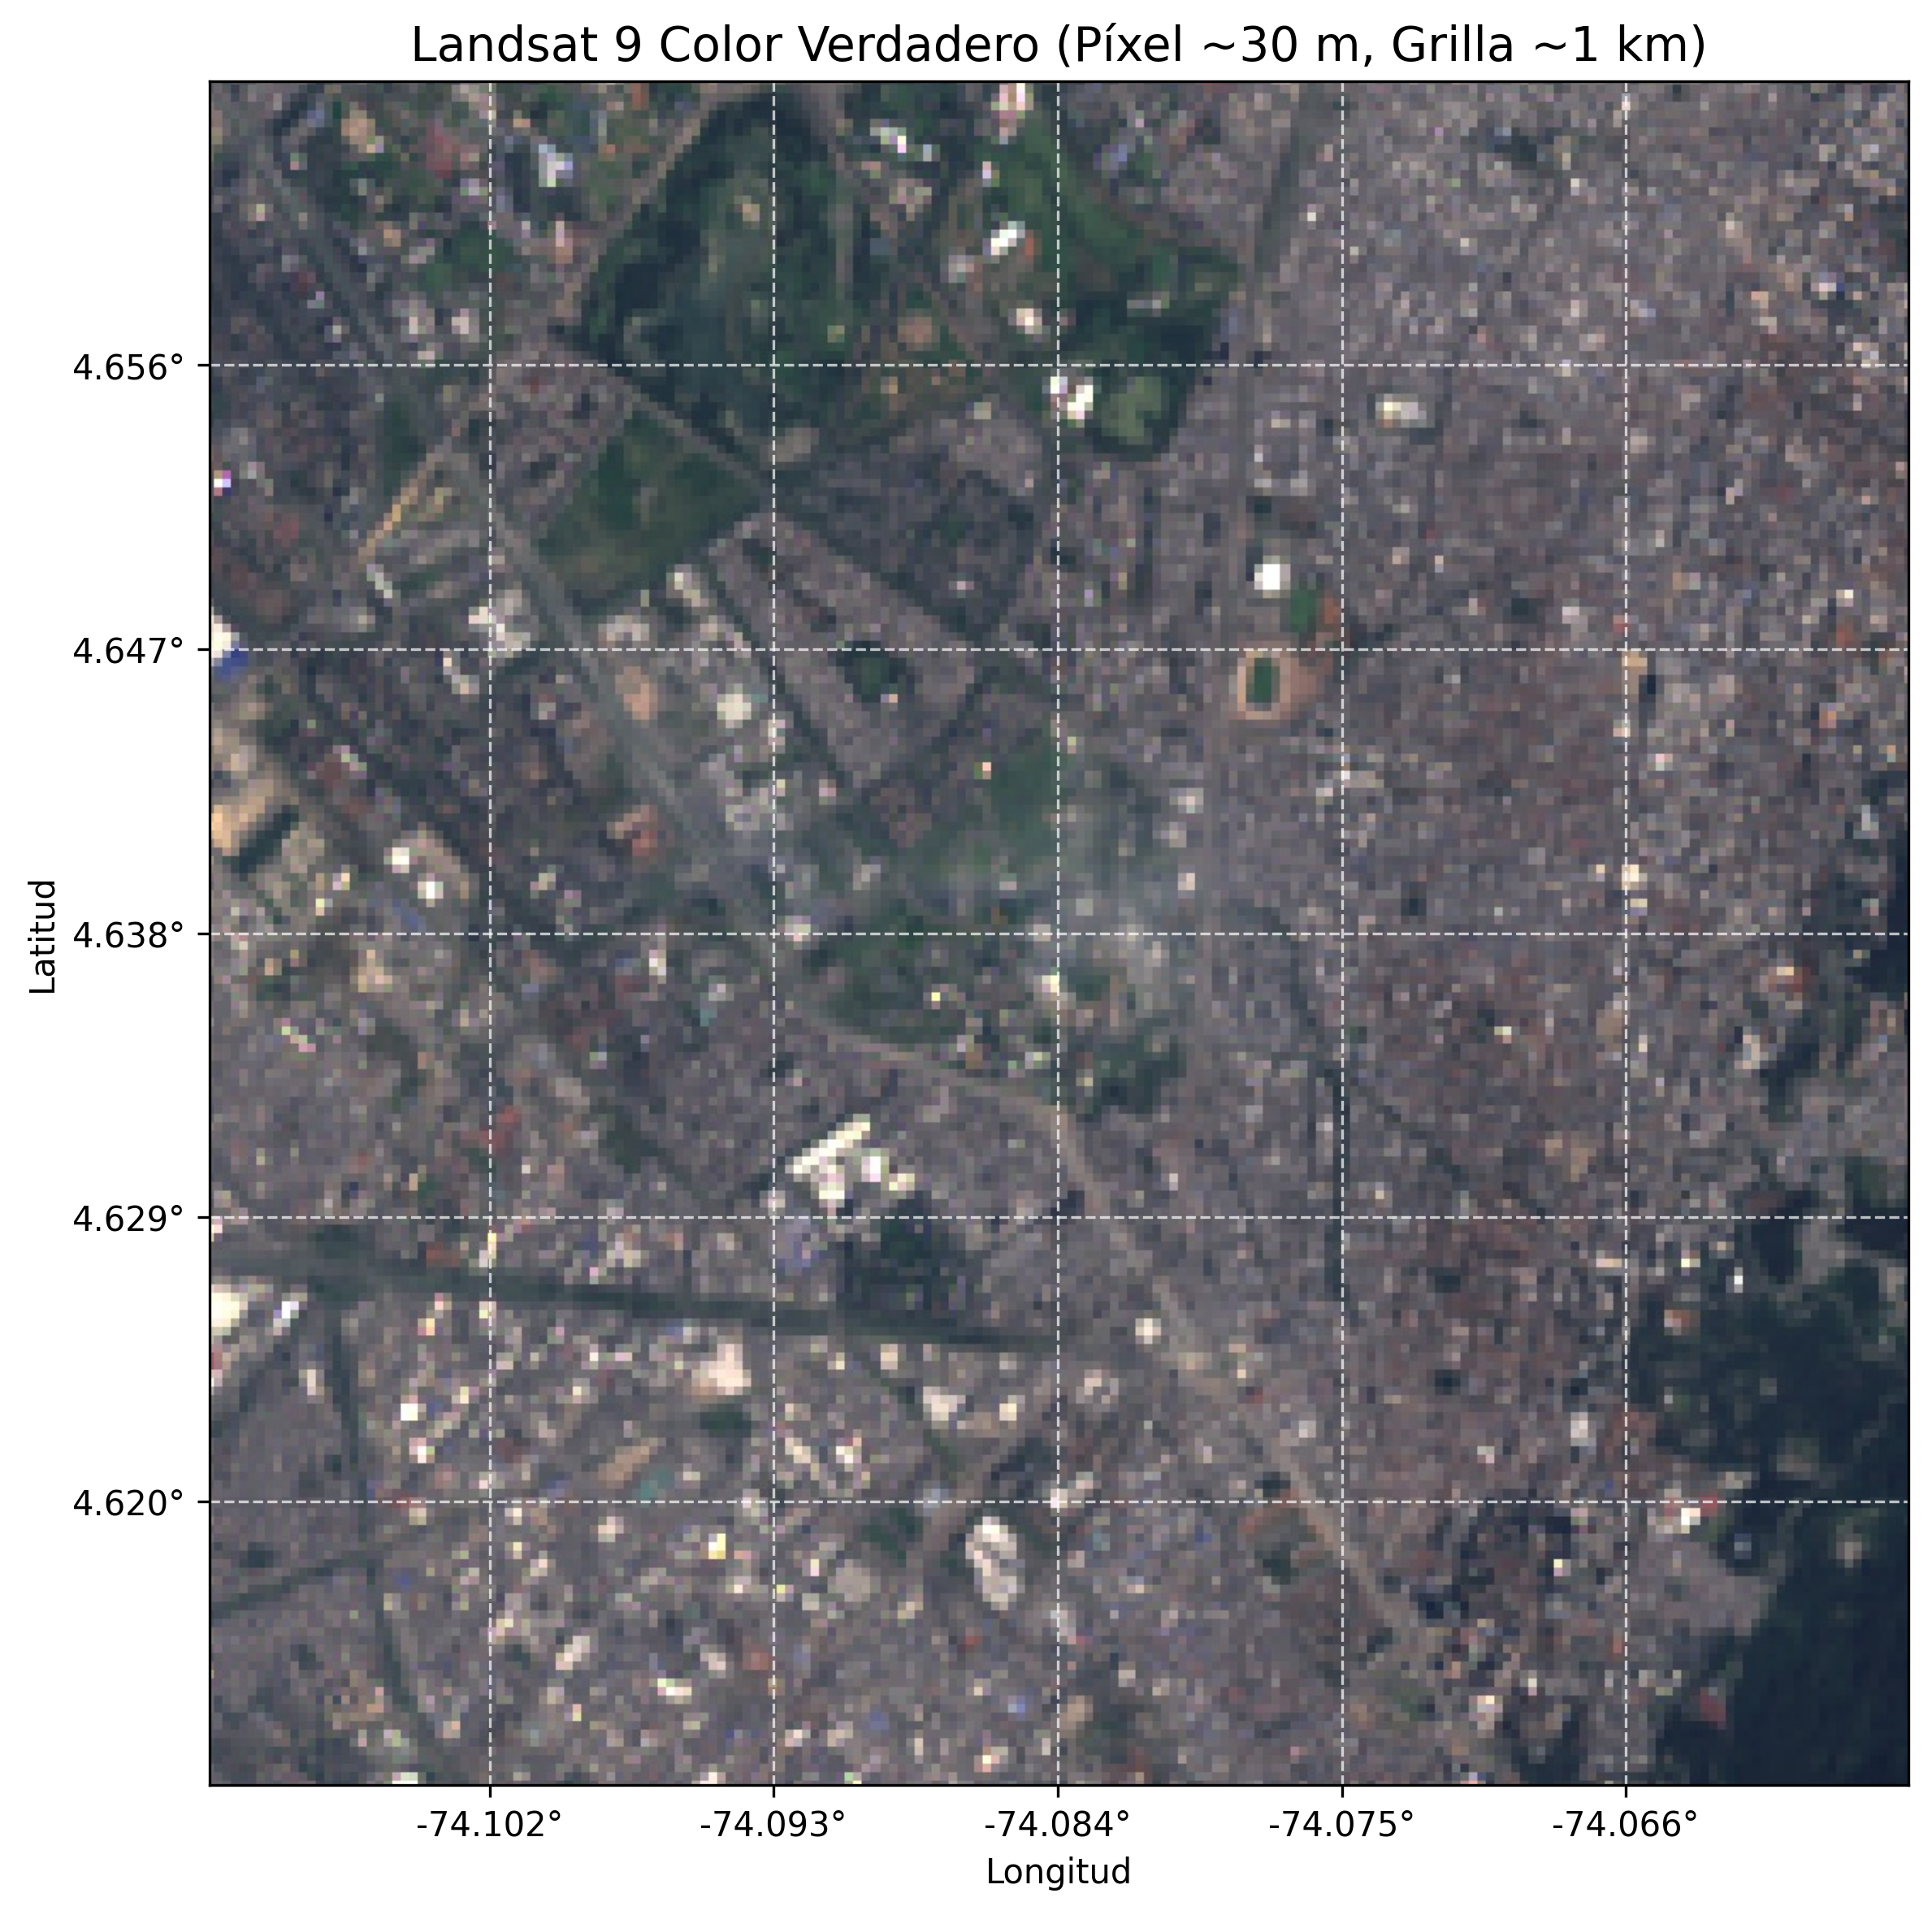
\includegraphics{45-practica_5_clase6_introduccion_sr_gee_files/figure-pdf/fig-python_landsat_estatico-output-1.png}

}

\caption{\label{fig-python_landsat_estatico}Imagen estática del Catálogo
Landsat 9 en color verdadero.}

\end{figure}%

\subsection{Javascript}

Para ejecutar este código, debes abrir el
\textbf{\href{https://code.earthengine.google.com/}{Code Editor de
Google Earth Engine}} en tu navegador, pegar el siguiente fragmento en
la consola central y hacer clic en \textbf{``Run''}.

\phantomsection\label{js_landsat}%
\begin{Shaded}
\begin{Highlighting}[]
\CommentTok{// 1. DEFINICIÓN DEL PUNTO GEOGRÁFICO}
\CommentTok{// En la interfaz de JavaScript de GEE el orden es [LONGITUD, LATITUD].}
\KeywordTok{var}\NormalTok{ punto\_unal }\OperatorTok{=}\NormalTok{ ee}\OperatorTok{.}\AttributeTok{Geometry}\OperatorTok{.}\FunctionTok{Point}\NormalTok{([}\OperatorTok{{-}}\FloatTok{74.084}\OperatorTok{,} \FloatTok{4.638}\NormalTok{])}\OperatorTok{;}

\CommentTok{// 2. CENTRAR EL VISOR}
\CommentTok{// Centramos el mapa interactivo en nuestro punto con un zoom de 17.}
\BuiltInTok{Map}\OperatorTok{.}\FunctionTok{centerObject}\NormalTok{(punto\_unal}\OperatorTok{,} \DecValTok{17}\NormalTok{)}\OperatorTok{;}

\CommentTok{// 3. CONSULTA Y FILTRADO DE DATOS}
\CommentTok{// Encadenamos funciones para obtener la imagen más limpia del catálogo:}
\KeywordTok{var}\NormalTok{ l9 }\OperatorTok{=}\NormalTok{ ee}\OperatorTok{.}\FunctionTok{ImageCollection}\NormalTok{(}\StringTok{"LANDSAT/LC09/C02/T1\_TOA"}\NormalTok{) }\CommentTok{// Carga la colección Landsat 9}
  \OperatorTok{.}\FunctionTok{filterBounds}\NormalTok{(punto\_unal)               }\CommentTok{// Filtro por ubicación (Bogotá)}
  \OperatorTok{.}\FunctionTok{filterDate}\NormalTok{(}\StringTok{\textquotesingle{}2023{-}01{-}01\textquotesingle{}}\OperatorTok{,} \StringTok{\textquotesingle{}2023{-}12{-}31\textquotesingle{}}\NormalTok{) }\CommentTok{// Filtro por periodo de tiempo (Año 2023)}
  \OperatorTok{.}\FunctionTok{sort}\NormalTok{(}\StringTok{\textquotesingle{}CLOUD\_COVER\textquotesingle{}}\NormalTok{)                    }\CommentTok{// Ordena por el metadato de nubosidad (Menor a Mayor)}
  \OperatorTok{.}\FunctionTok{first}\NormalTok{()}\OperatorTok{;}                               \CommentTok{// Selecciona la primera de la lista (la más despejada)}

\CommentTok{// 4. PARÁMETROS DE VISUALIZACIÓN}
\CommentTok{// Definimos el diccionario de visualización para ver bandas B4, B3 y B2.}
\KeywordTok{var}\NormalTok{ visParams }\OperatorTok{=}\NormalTok{ \{}\DataTypeTok{bands}\OperatorTok{:}\NormalTok{ [}\StringTok{\textquotesingle{}B4\textquotesingle{}}\OperatorTok{,} \StringTok{\textquotesingle{}B3\textquotesingle{}}\OperatorTok{,} \StringTok{\textquotesingle{}B2\textquotesingle{}}\NormalTok{]}\OperatorTok{,} \DataTypeTok{min}\OperatorTok{:} \FloatTok{0.0}\OperatorTok{,} \DataTypeTok{max}\OperatorTok{:} \FloatTok{0.3}\NormalTok{\}}\OperatorTok{;}

\CommentTok{// 5. MOSTRAR EN PANTALLA Y EN CONSOLA}
\CommentTok{// Añadimos la imagen procesada como una capa en el Code Editor.}
\BuiltInTok{Map}\OperatorTok{.}\FunctionTok{addLayer}\NormalTok{(l9}\OperatorTok{,}\NormalTok{ visParams}\OperatorTok{,} \StringTok{\textquotesingle{}Landsat 9 {-} UNAL Bogotá\textquotesingle{}}\NormalTok{)}\OperatorTok{;}

\CommentTok{// Imprimimos los metadatos de la imagen en la consola de la derecha}
\FunctionTok{print}\NormalTok{(}\StringTok{\textquotesingle{}Metadatos de la imagen seleccionada:\textquotesingle{}}\OperatorTok{,}\NormalTok{ l9)}\OperatorTok{;}
\CommentTok{// Imprimimos el ID exacto para poder usarlo en ArcGIS Pro / QGIS}
\FunctionTok{print}\NormalTok{(}\StringTok{\textquotesingle{}ID exacto de la imagen:\textquotesingle{}}\OperatorTok{,}\NormalTok{ l9}\OperatorTok{.}\FunctionTok{get}\NormalTok{(}\StringTok{\textquotesingle{}system:id\textquotesingle{}}\NormalTok{))}\OperatorTok{;}
\end{Highlighting}
\end{Shaded}

\begin{center}\rule{0.5\linewidth}{0.5pt}\end{center}

\phantomsection\label{js_landsat_estatico}%
\begin{Shaded}
\begin{Highlighting}[]
\CommentTok{// ▷ CÓDIGO MAPA ESTÁTICO (THUMBNAIL) EN JAVASCRIPT (Independiente)}

\CommentTok{// 1. DEFINICIÓN DEL PUNTO Y REGIÓN DE INTERÉS}
\KeywordTok{var}\NormalTok{ punto\_unal }\OperatorTok{=}\NormalTok{ ee}\OperatorTok{.}\AttributeTok{Geometry}\OperatorTok{.}\FunctionTok{Point}\NormalTok{([}\OperatorTok{{-}}\FloatTok{74.084}\OperatorTok{,} \FloatTok{4.638}\NormalTok{])}\OperatorTok{;}
\KeywordTok{var}\NormalTok{ region\_interes }\OperatorTok{=}\NormalTok{ punto\_unal}\OperatorTok{.}\FunctionTok{buffer}\NormalTok{(}\DecValTok{3000}\NormalTok{)}\OperatorTok{;} \CommentTok{// Buffer de 3km}

\CommentTok{// 2. CONSULTA Y SELECCIÓN DE LA IMAGEN}
\KeywordTok{var}\NormalTok{ l9\_estatica }\OperatorTok{=}\NormalTok{ ee}\OperatorTok{.}\FunctionTok{ImageCollection}\NormalTok{(}\StringTok{"LANDSAT/LC09/C02/T1\_TOA"}\NormalTok{)}
  \OperatorTok{.}\FunctionTok{filterBounds}\NormalTok{(punto\_unal)}
  \OperatorTok{.}\FunctionTok{filterDate}\NormalTok{(}\StringTok{\textquotesingle{}2023{-}01{-}01\textquotesingle{}}\OperatorTok{,} \StringTok{\textquotesingle{}2023{-}12{-}31\textquotesingle{}}\NormalTok{)}
  \OperatorTok{.}\FunctionTok{sort}\NormalTok{(}\StringTok{\textquotesingle{}CLOUD\_COVER\textquotesingle{}}\NormalTok{)}
  \OperatorTok{.}\FunctionTok{first}\NormalTok{()}\OperatorTok{;}

\CommentTok{// 3. PARÁMETROS DE VISUALIZACIÓN}
\KeywordTok{var}\NormalTok{ visParamsEstatica }\OperatorTok{=}\NormalTok{ \{}
  \DataTypeTok{bands}\OperatorTok{:}\NormalTok{ [}\StringTok{\textquotesingle{}B4\textquotesingle{}}\OperatorTok{,} \StringTok{\textquotesingle{}B3\textquotesingle{}}\OperatorTok{,} \StringTok{\textquotesingle{}B2\textquotesingle{}}\NormalTok{]}\OperatorTok{,}
  \DataTypeTok{min}\OperatorTok{:} \FloatTok{0.0}\OperatorTok{,}
  \DataTypeTok{max}\OperatorTok{:} \FloatTok{0.3}\OperatorTok{,}
  \DataTypeTok{dimensions}\OperatorTok{:} \DecValTok{800}\OperatorTok{,}
  \DataTypeTok{region}\OperatorTok{:}\NormalTok{ region\_interes}
\NormalTok{\}}\OperatorTok{;}

\CommentTok{// 4. MOSTRAR EN CONSOLA LA URL Y EL THUMBNAIL}
\FunctionTok{print}\NormalTok{(}\StringTok{\textquotesingle{}URL de la imagen PNG:\textquotesingle{}}\OperatorTok{,}\NormalTok{ l9\_estatica}\OperatorTok{.}\FunctionTok{getThumbURL}\NormalTok{(visParamsEstatica))}\OperatorTok{;}

\KeywordTok{var}\NormalTok{ miniatura }\OperatorTok{=}\NormalTok{ ui}\OperatorTok{.}\FunctionTok{Thumbnail}\NormalTok{(\{}
  \DataTypeTok{image}\OperatorTok{:}\NormalTok{ l9\_estatica}\OperatorTok{,}
  \DataTypeTok{params}\OperatorTok{:}\NormalTok{ visParamsEstatica}\OperatorTok{,}
  \DataTypeTok{style}\OperatorTok{:}\NormalTok{ \{}\DataTypeTok{width}\OperatorTok{:} \StringTok{\textquotesingle{}400px\textquotesingle{}}\OperatorTok{,} \DataTypeTok{height}\OperatorTok{:} \StringTok{\textquotesingle{}400px\textquotesingle{}}\NormalTok{\}}
\NormalTok{\})}\OperatorTok{;}
\FunctionTok{print}\NormalTok{(}\StringTok{\textquotesingle{}Vista previa estática:\textquotesingle{}}\OperatorTok{,}\NormalTok{ miniatura)}\OperatorTok{;}
\end{Highlighting}
\end{Shaded}

\begin{center}\rule{0.5\linewidth}{0.5pt}\end{center}

\section{GEE desde QGIS (Plugin de Google Earth
Engine)}\label{gee-desde-qgis-plugin-de-google-earth-engine}

Ya vimos cómo ejecutar código en Python y JavaScript. Ahora exploraremos
cómo integrar toda esta potencia directamente dentro de una interfaz SIG
tradicional como \textbf{QGIS}, utilizando el plugin de GEE.

Abre QGIS, asegúrate de tener el plugin instalado y actualizado (Ver
Sección~\ref{sec-qgis-gee-pixi}.) y sigue estos tres pasos:

\subsection{Búsqueda en el Catálogo desde
QGIS}\label{buxfasqueda-en-el-catuxe1logo-desde-qgis}

Ve al panel del plugin de GEE. En la pestaña \textbf{Search}, puedes
buscar colecciones de imágenes directamente por su nombre o ID. Intenta
buscar la colección que usamos arriba
(\texttt{LANDSAT/LC09/C02/T1\_TOA}).

\begin{figure}

\centering{

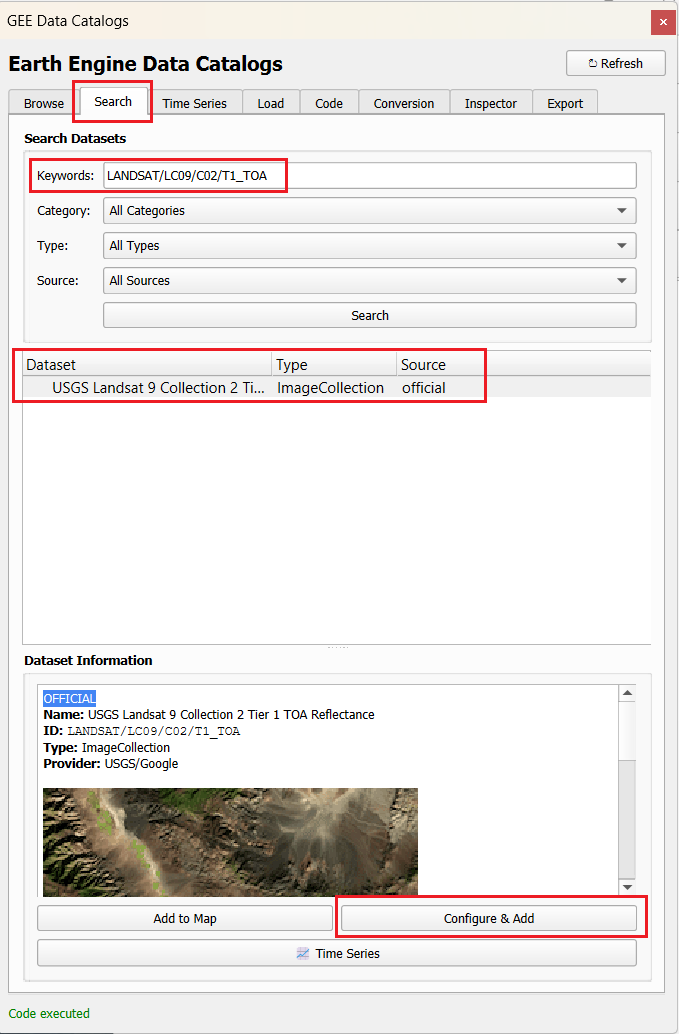
\includegraphics[width=0.8\textwidth,height=\textheight]{images/qgis/qgis_plugin_gee_tab_search.png}

}

\caption{\label{fig-qgis-search}Búsqueda de colecciones en el plugin de
GEE para QGIS.}

\end{figure}%

\subsection{Ejecutar Código de
Geemap}\label{ejecutar-cuxf3digo-de-geemap}

Ahora, abre la pestaña \textbf{Code}. Copia exactamente el código de
Python que vimos en la sección anterior (el de la pestaña \emph{CÓDIGO
GEEMAP QGIS}) y pégalo allí. Haz clic en ejecutar.

\begin{tcolorbox}[enhanced jigsaw, opacityback=0, left=2mm, colbacktitle=quarto-callout-warning-color!10!white, leftrule=.75mm, breakable, titlerule=0mm, rightrule=.15mm, bottomrule=.15mm, arc=.35mm, colback=white, colframe=quarto-callout-warning-color-frame, opacitybacktitle=0.6, toptitle=1mm, title={⚠️ ¡Atención con la navegación!}, bottomtitle=1mm, toprule=.15mm, coltitle=black]

La imagen se cargará en tus capas de QGIS, pero \textbf{nota
importante:} a diferencia del visor web, la imagen probablemente
\textbf{no cargará centrada} de forma automática en tu lienzo. Tendrás
que hacer clic derecho sobre la capa generada y seleccionar ``Acercar a
la capa'' (Zoom to layer).

\end{tcolorbox}

\begin{figure}

\centering{

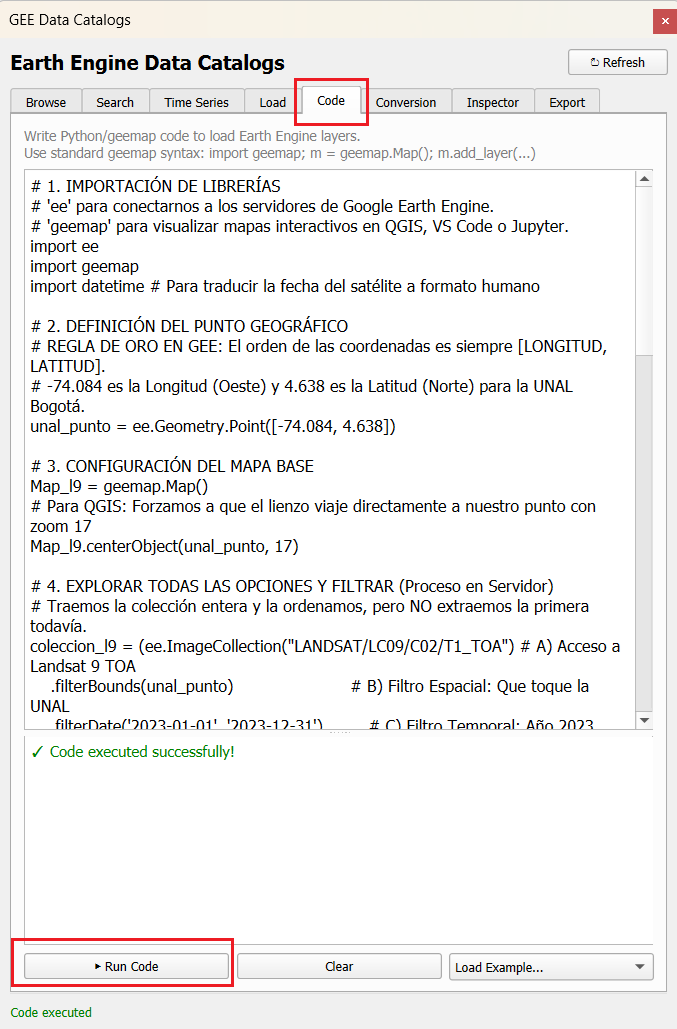
\includegraphics[width=0.8\textwidth,height=\textheight]{images/qgis/qgis_plugin_gee_tab_code.png}

}

\caption{\label{fig-qgis-code}Ejecución de scripts Python directamente
en QGIS.}

\end{figure}%

\subsection{El Reto: Cargar Parámetros
Manualmente}\label{el-reto-cargar-paruxe1metros-manualmente}

Finalmente, ve a la pestaña \textbf{Load}. Aquí puedes cargar imágenes
sin necesidad de programar, simplemente rellenando los campos.

\textbf{🎯 Tu reto:} Utilizando la información de metadatos (ID del
archivo exacto) y los parámetros de visualización (bandas B4, B3, B2,
min y max) que descubriste corriendo el código anterior, llena este
formulario. ¡Intenta cargar \textbf{exactamente la misma imagen} que
obtuvimos por código, pero esta vez configurándola manualmente desde
esta interfaz!

\begin{figure}

\centering{

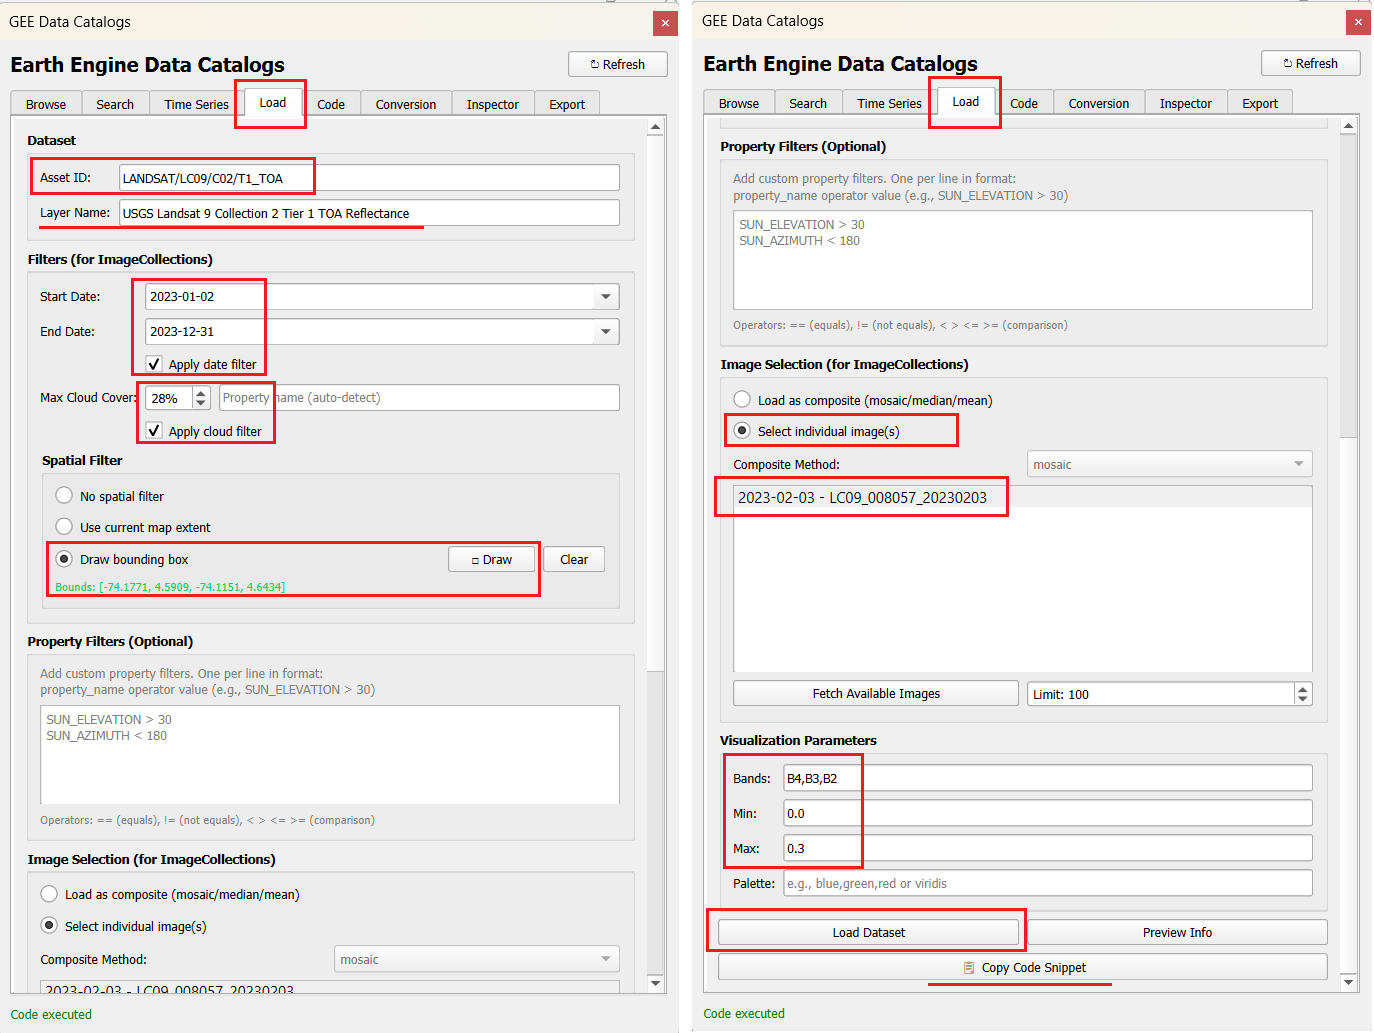
\includegraphics[width=1\textwidth,height=\textheight]{images/qgis/qgis_plugin_gee_tab_load.png}

}

\caption{\label{fig-qgis-load}Carga manual de imágenes usando parámetros
específicos.}

\end{figure}%

\begin{quote}
Puede usar múltiples propiedades de imagen para filtrar la búsqueda en
la pestaña \texttt{Property\ Filters\ (Optional)}. Escriba en cada línea
de la caja de texto disponible, filtros personalizados. Ej:
\texttt{SUN\_ELEVATION\ \textgreater{}\ 30} y
\texttt{SUN\_AZIMUTH\ \textless{}\ 180}. La lista de propiedades se
puede obtener del
\href{https://developers.google.com/earth-engine/datasets/catalog/}{catálogo
de GEE}.

\begin{itemize}
\tightlist
\item
  Busque el \texttt{Asset\ ID}. Léalo del código Python provisto:
  \texttt{ee.ImageCollection("LANDSAT/LC09/C02/T1\_TOA")}
\item
  En la pestaña \texttt{Image\ Properties} estudie el nombre, tipo y
  descripción de las propiedades de las imágenes que se pueden usar para
  filtrar el grupo de datos Landsat. Vea la figura
  Figura~\ref{fig-gee-catalog-props} a continuación.
\end{itemize}
\end{quote}

\begin{figure}

\centering{

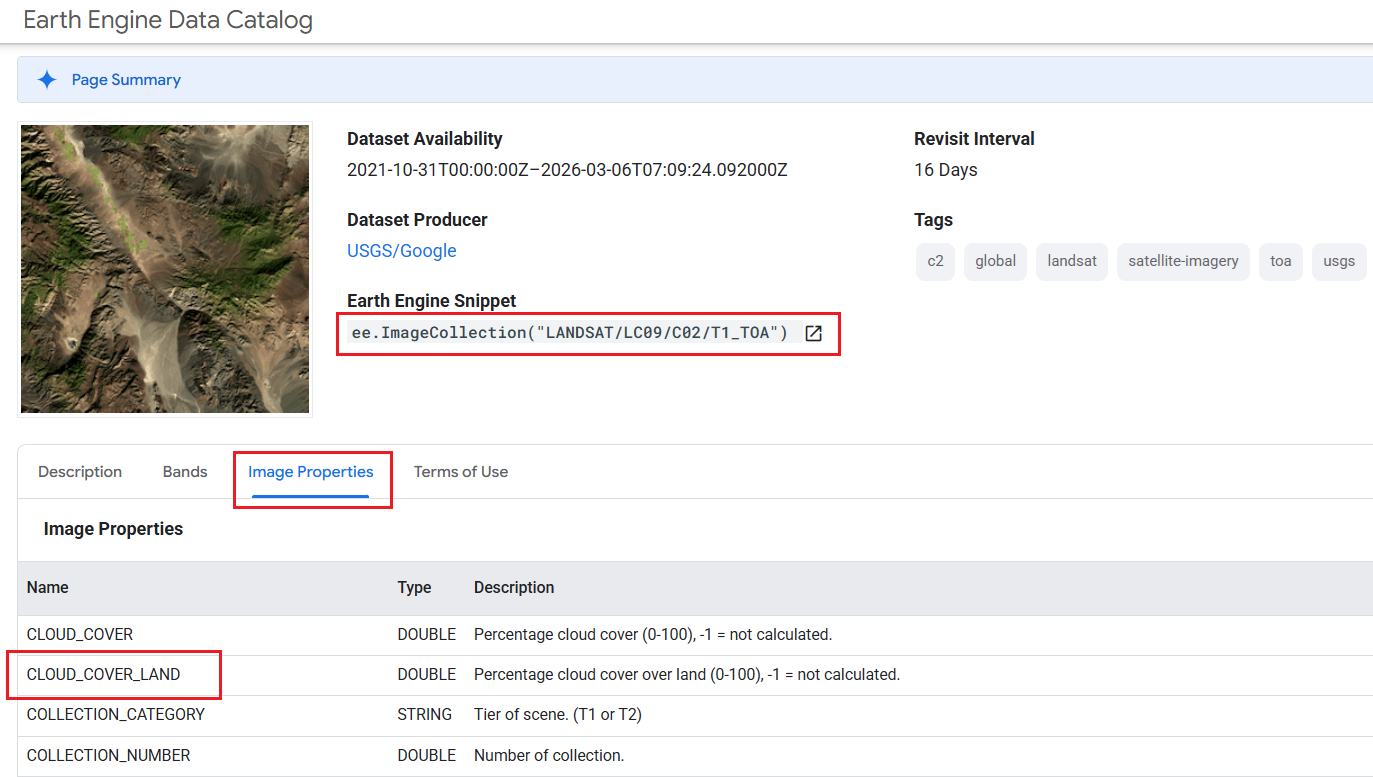
\includegraphics[width=1\textwidth,height=\textheight]{images/sensores_remotos/gee_catalog_image_properties.png}

}

\caption{\label{fig-gee-catalog-props}Propiedades de la imagen en el
Catálogo de GEE.}

\end{figure}%

\section{GEE desde ArcGIS PRO (caja de
herramientas)}\label{sec-arcgis-pro-gee-start}

La caja de herramientas de GEE (\emph{GEE Toolbox}) actúa como un puente
que no requiere programación entre GEE y ArcGIS Pro. Te permite llevar
bases de datos, herramientas y resultados de Google directamente a tu
software de escritorio para análisis adicionales o presentación de
resultados. Sus capacidades incluyen:

\begin{itemize}
\tightlist
\item
  Explorar, filtrar y descargar datos directamente desde el Catálogo de
  Datos de GEE.
\item
  Añadir colecciones de imágenes o vectores a tu mapa de ArcGIS Pro
  usando un simple \emph{Asset ID} (Identificador de archivo) extraído
  del catálogo de Google.
\item
  Integrar operaciones de GEE en \emph{ModelBuilder} y ejecutar scripts
  de Python que llamen a las funciones de GEE directamente dentro del
  entorno de ArcGIS Pro.
\end{itemize}

\textbf{Guías de inicio recomendadas:}

\begin{itemize}
\tightlist
\item
  \href{https://github.com/gee-community/arcgis-earthengine-toolbox/blob/main/docs/01_quick_start.md}{ArcGIS
  Earth Engine Toolbox (GEE Connector) User Guide: Quick Start}
\item
  \href{https://storymaps.arcgis.com/stories/bf22d27bfceb4507a40b4a52e5dec702}{Bring
  Google Earth Engine's Data Right into ArcGIS Pro}
\end{itemize}

\textbf{Recursos adicionales:}

\begin{itemize}
\tightlist
\item
  \href{https://github.com/gee-community/arcgis-earthengine-toolbox/tree/main/docs}{Todas
  las guías oficiales}
\item
  \href{https://www.youtube.com/@zhifeidong4310/videos}{Video guías}
\item
  Artículo en Medium:
  \href{https://medium.com/google-earth/bridging-worlds-bringing-google-earth-engine-to-desktop-gis-users-3f2edb99131d}{Bridging
  Worlds: Bringing Google Earth Engine to Desktop GIS Users!}
\end{itemize}

\begin{figure}

\centering{

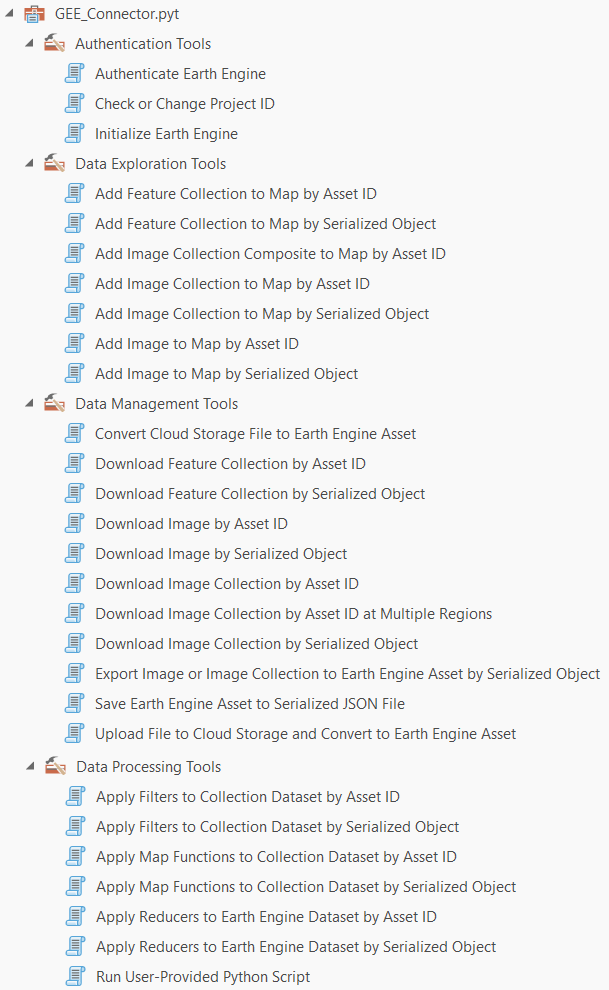
\includegraphics[width=0.6\textwidth,height=\textheight]{images/arcgispro/gee/gee_arcgispro_tool.png}

}

\caption{\label{fig-gee-tool}Caja de Herramientas GEE dentro de ArcGIS
Pro.}

\end{figure}%

\subsection{Inicializar GEE en ArcGIS
Pro}\label{sec-arcgis-pro-initialize-gee}

Asegúrate de seguir el procedimiento de instalación y configuración de
GEE en ArcGIS Pro en Sección~\ref{sec-arcgis-pro-gee}.

Antes de usar cualquier función, debemos autenticar nuestra cuenta. En
la caja de herramientas de GEE dentro de ArcGIS Pro, abra la sección
\texttt{Authentication\ Tools}:

\begin{figure}

\centering{

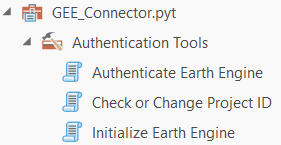
\includegraphics[width=0.3\textwidth,height=\textheight]{images/arcgispro/gee/opciones_inicializacion_gee.png}

}

\caption{\label{fig-arcgis-auth-tools}Herramientas de Autenticación de
GEE en ArcGIS Pro.}

\end{figure}%

\textbf{Paso A:} Abra la herramienta
\texttt{Authenticate\ Earth\ Engine} y escriba su \emph{Project ID} (ej.
\texttt{ee-giswqg}). Al ejecutar (\texttt{Run}) la herramienta y ver los
detalles de la ejecución (\texttt{View\ Details}), deberá observar un
mensaje de éxito como: \emph{Earth Engine is ready to use.
Authentication successful}.

\begin{figure}

\centering{

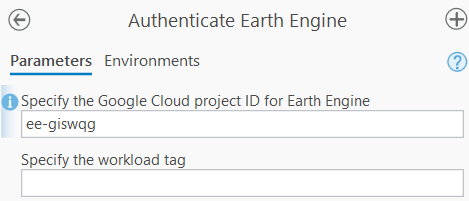
\includegraphics[width=0.4\textwidth,height=\textheight]{images/arcgispro/gee/gee_authenticate_pro.png}

}

\caption{\label{fig-arcgis-auth-success}Herramienta de autenticación en
GEE (Recuerda cambiar el Project ID por el tuyo).}

\end{figure}%

\textbf{Paso B:} A continuación, abra la herramienta
\texttt{Initialize\ Earth\ Engine} y escriba nuevamente su \emph{Project
ID}. Ejecute la herramienta; en los detalles observará el mensaje
confirmando: \emph{Earth Engine is ready to use.}

\subsection{Exploración del Catálogo y
Propiedades}\label{exploraciuxf3n-del-catuxe1logo-y-propiedades}

Al igual que hicimos en QGIS, usaremos la herramienta
\texttt{Add\ Image\ Collection\ to\ Map\ by\ Asset\ ID} para cargar
nuestra imagen Landsat de la Universidad Nacional. Para hacerlo
correctamente:

\begin{itemize}
\tightlist
\item
  En el
  \href{https://developers.google.com/earth-engine/datasets/catalog/}{catálogo
  de GEE} busque el \texttt{Asset\ ID} de la imagen a cargar. Léalo del
  código Python provisto en las secciones anteriores:
  \texttt{ee.ImageCollection("LANDSAT/LC09/C02/T1\_TOA")}.
\item
  En la pestaña \texttt{Image\ Properties} del catálogo (ver figura
  Figura~\ref{fig-gee-catalog-props}), estudie el nombre, tipo y
  descripción de las propiedades que permiten filtrar el conjunto de
  datos.
\item
  Para filtrar específicamente por el porcentaje de nubes sobre tierra
  firme, debe usar la propiedad \texttt{CLOUD\_COVER\_LAND}.
\end{itemize}

\subsection{El Reto: Añadir la Colección al
Mapa}\label{el-reto-auxf1adir-la-colecciuxf3n-al-mapa}

Con toda la información recolectada, es hora de ponerla en práctica en
la interfaz de ArcGIS Pro:

\begin{itemize}
\tightlist
\item
  Acérquese (haga zoom) al campus de la Universidad Nacional en su mapa
  base de ArcGIS.
\item
  Abra la herramienta
  \texttt{Add\ Image\ Collection\ to\ Map\ by\ Asset\ ID}.
\item
  Llene cada uno de los campos de acuerdo con el código utilizado
  anteriormente o verifique la Figura~\ref{fig-arcgis-add-collection}
  que se encuentra a continuación.
\item
  Seleccione la imagen a cargar de la lista desplegable
  \texttt{Select\ an\ image}. \textbf{Nota de verificación}: Una vez
  todos los parámetros están correctamente definidos, solo una imagen
  debería aparecer en la lista desplegable.
\item
  Presione el botón \texttt{run}
\end{itemize}

\begin{figure}

\centering{

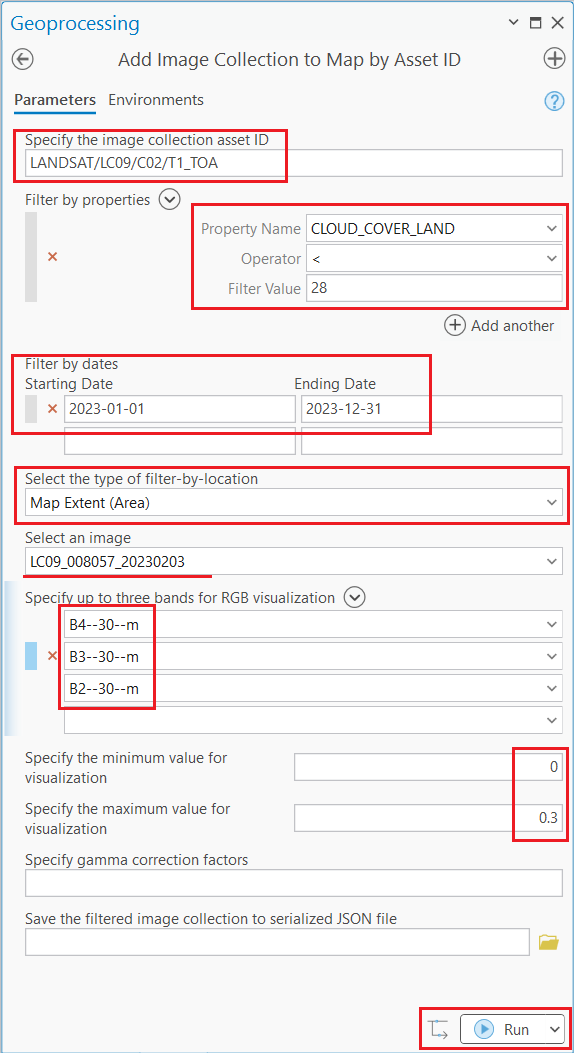
\includegraphics[width=0.6\textwidth,height=\textheight]{images/arcgispro/gee/add_image_collection_to_map_by_asset_id.png}

}

\caption{\label{fig-arcgis-add-collection}Uso de la herramienta Add
Image Collection to Map by Asset ID.}

\end{figure}%

\begin{quote}
\textbf{💡 Tip:} Puede usar múltiples propiedades de imagen para refinar
la búsqueda dentro de esta herramienta. En la sección
\texttt{Filter\ by\ properties}, haga clic en \texttt{Add\ another} y
rellene adecuadamente los parámetros \texttt{Property\ Name},
\texttt{Operator} y \texttt{Filter\ Value}.
\end{quote}

\subsection{Añadir imagen mediante JSON (Serialized
Object)}\label{auxf1adir-imagen-mediante-json-serialized-object}

Utilice el archivo \texttt{landsat9\_serializado.json} que generamos y
descargamos en el paso anterior para cargar la imagen en ArcGIS Pro.
Para ello, abra la herramienta \textbf{Add Image to Map by Serialized
Object}, busque su archivo en el disco y ejecute la herramienta.

Puede guiarse con la configuración mostrada en la figura
Figura~\ref{fig-arcgis-serialized}.

\begin{figure}

\centering{

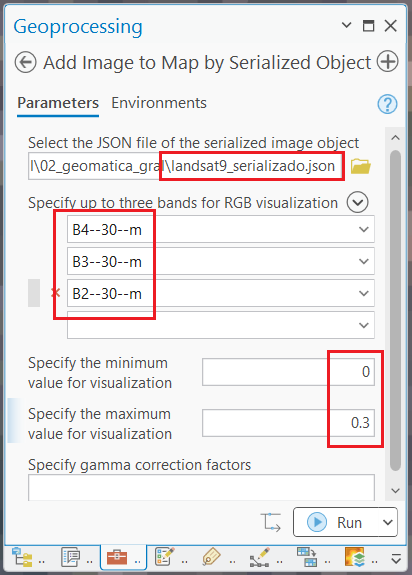
\includegraphics[width=0.5\textwidth,height=\textheight]{images/arcgispro/gee/add_image_to_map_by_serialized_object.png}

}

\caption{\label{fig-arcgis-serialized}Uso de la herramienta Add Image to
Map by Serialized Object en ArcGIS Pro.}

\end{figure}%

\subsection{Añadir imagen mediante Asset
ID}\label{auxf1adir-imagen-mediante-asset-id}

Alternativamente, si no quiere usar el JSON, puede utilizar el
identificador único y exacto de la escena. Copie el ID
\texttt{LANDSAT/LC09/C02/T1\_TOA/LC09\_008057\_20230203} (que imprimimos
previamente en la consola usando nuestro código Python) y úselo para
cargar la imagen mediante la herramienta \textbf{Add Image to Map by
Asset ID}.

Vea la figura Figura~\ref{fig-arcgis-assetid} como referencia para
rellenar los parámetros.

\begin{figure}

\centering{

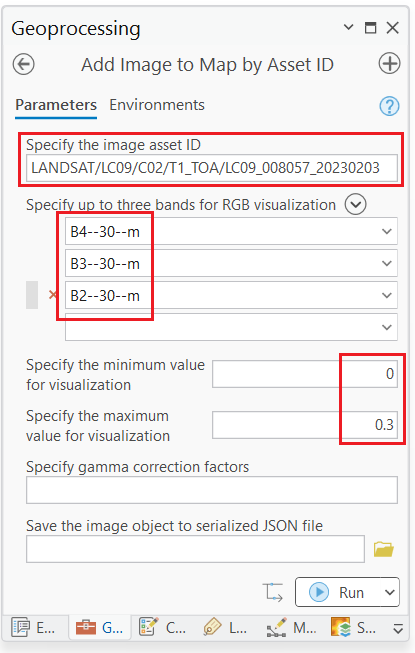
\includegraphics[width=0.5\textwidth,height=\textheight]{images/arcgispro/gee/add_image_to_map_by_asset_id.png}

}

\caption{\label{fig-arcgis-assetid}Uso de la herramienta Add Image to
Map by Asset ID en ArcGIS Pro.}

\end{figure}%

\begin{center}\rule{0.5\linewidth}{0.5pt}\end{center}

\section{Catálogo de datos: Sentinel
2}\label{catuxe1logo-de-datos-sentinel-2}

Para este segundo ejercicio exploraremos la constelación Sentinel-2 de
la Agencia Espacial Europea (ESA) bajo el programa Copernicus. Este
satélite ofrece una resolución espacial superior (10 metros en sus
bandas visibles) y es ideal para el monitoreo agrícola y de coberturas.

\begin{longtable}[]{@{}lll@{}}
\toprule\noalign{}
Banda & Resolución & Descripción \\
\midrule\noalign{}
\endhead
\bottomrule\noalign{}
\endlastfoot
B2, B3, B4 & 10m & Azul, Verde, Rojo (Espectro Visible) \\
B8 & 10m & Infrarrojo Cercano (NIR) \\
\end{longtable}

\subsection{Entendiendo la colección y el
código}\label{entendiendo-la-colecciuxf3n-y-el-cuxf3digo-1}

El flujo de trabajo es idéntico al que utilizamos con Landsat, pero con
dos diferencias importantes:

\begin{enumerate}
\def\labelenumi{\arabic{enumi}.}
\tightlist
\item
  El \emph{Asset ID} de la colección es
  \texttt{COPERNICUS/S2\_SR\_HARMONIZED}.
\item
  El metadato para filtrar nubes en Sentinel 2 se llama
  \texttt{CLOUDY\_PIXEL\_PERCENTAGE} (a diferencia de Landsat que usa
  \texttt{CLOUD\_COVER}).
\item
  El rango de valores de reflectancia (\texttt{min} y \texttt{max})
  cambia. Mientras Landsat 9 TOA va de 0 a 1 (usamos 0 a 0.3), los
  productos de Sentinel 2 SR vienen escalados por defecto entre 0 y
  10000. Por eso, en los parámetros visuales usaremos
  \texttt{max:\ 3000}.
\end{enumerate}

\subsection{Python}

\begin{Shaded}
\begin{Highlighting}[]
\CommentTok{\# \#| eval: false}

\CommentTok{\# Código usando Folium!}

\ImportTok{import}\NormalTok{ ee}
\ImportTok{import}\NormalTok{ folium}
\ImportTok{import}\NormalTok{ datetime}
\ImportTok{import}\NormalTok{ json }

\CommentTok{\# 1. DEFINICIÓN DEL PUNTO GEOGRÁFICO}
\NormalTok{unal\_punto }\OperatorTok{=}\NormalTok{ ee.Geometry.Point([}\OperatorTok{{-}}\FloatTok{74.084}\NormalTok{, }\FloatTok{4.638}\NormalTok{])}

\CommentTok{\# 2. EXPLORAR TODAS LAS OPCIONES Y FILTRAR}
\NormalTok{coleccion\_s2 }\OperatorTok{=}\NormalTok{ (ee.ImageCollection(}\StringTok{"COPERNICUS/S2\_SR\_HARMONIZED"}\NormalTok{) }
\NormalTok{    .filterBounds(unal\_punto) }
\NormalTok{    .filterDate(}\StringTok{\textquotesingle{}2023{-}01{-}01\textquotesingle{}}\NormalTok{, }\StringTok{\textquotesingle{}2023{-}12{-}31\textquotesingle{}}\NormalTok{) }
\NormalTok{    .}\BuiltInTok{filter}\NormalTok{(ee.Filter.lt(}\StringTok{\textquotesingle{}CLOUDY\_PIXEL\_PERCENTAGE\textquotesingle{}}\NormalTok{, }\DecValTok{10}\NormalTok{))}
\NormalTok{    .sort(}\StringTok{\textquotesingle{}CLOUDY\_PIXEL\_PERCENTAGE\textquotesingle{}}\NormalTok{))}

\CommentTok{\# 3. DIAGNÓSTICO: EXTRAER EL TOP 3 DE IMÁGENES}
\NormalTok{ids }\OperatorTok{=}\NormalTok{ coleccion\_s2.aggregate\_array(}\StringTok{\textquotesingle{}system:id\textquotesingle{}}\NormalTok{).getInfo()}
\NormalTok{nubes }\OperatorTok{=}\NormalTok{ coleccion\_s2.aggregate\_array(}\StringTok{\textquotesingle{}CLOUDY\_PIXEL\_PERCENTAGE\textquotesingle{}}\NormalTok{).getInfo()}
\NormalTok{fechas }\OperatorTok{=}\NormalTok{ coleccion\_s2.aggregate\_array(}\StringTok{\textquotesingle{}system:time\_start\textquotesingle{}}\NormalTok{).getInfo()}

\BuiltInTok{print}\NormalTok{(}\StringTok{"{-}{-}{-} TOP 3 IMÁGENES SENTINEL{-}2 CON MENOS NUBES (2023) {-}{-}{-}"}\NormalTok{)}
\ControlFlowTok{for}\NormalTok{ i }\KeywordTok{in} \BuiltInTok{range}\NormalTok{(}\BuiltInTok{min}\NormalTok{(}\DecValTok{3}\NormalTok{, }\BuiltInTok{len}\NormalTok{(ids))):}
\NormalTok{    fecha\_legible }\OperatorTok{=}\NormalTok{ datetime.datetime.fromtimestamp(fechas[i] }\OperatorTok{/} \FloatTok{1000.0}\NormalTok{, datetime.UTC).strftime(}\StringTok{\textquotesingle{}\%Y{-}\%m{-}}\SpecialCharTok{\%d}\StringTok{\textquotesingle{}}\NormalTok{)}
    \BuiltInTok{print}\NormalTok{(}\SpecialStringTok{f"Opción }\SpecialCharTok{\{}\NormalTok{i}\OperatorTok{+}\DecValTok{1}\SpecialCharTok{\}}\SpecialStringTok{ | Nubes: }\SpecialCharTok{\{}\NormalTok{nubes[i]}\SpecialCharTok{:.2f\}}\SpecialStringTok{\% | Fecha: }\SpecialCharTok{\{}\NormalTok{fecha\_legible}\SpecialCharTok{\}}\SpecialStringTok{"}\NormalTok{)}
    \BuiltInTok{print}\NormalTok{(}\SpecialStringTok{f"ID: }\SpecialCharTok{\{}\NormalTok{ids[i]}\SpecialCharTok{\}}\CharTok{\textbackslash{}n}\SpecialStringTok{"}\NormalTok{)}
\BuiltInTok{print}\NormalTok{(}\StringTok{"{-}{-}{-}{-}{-}{-}{-}{-}{-}{-}{-}{-}{-}{-}{-}{-}{-}{-}{-}{-}{-}{-}{-}{-}{-}{-}{-}{-}{-}{-}{-}{-}{-}{-}{-}{-}{-}{-}{-}{-}{-}{-}{-}{-}{-}{-}{-}{-}{-}{-}{-}{-}{-}{-}{-}{-}{-}{-}"}\NormalTok{)}

\CommentTok{\# 4. SELECCIÓN DEFINITIVA DE LA IMAGEN}
\NormalTok{s2 }\OperatorTok{=}\NormalTok{ ee.Image(coleccion\_s2.first())}

\CommentTok{\# 5. EXPORTAR LOS ARCHIVOS JSON (METADATOS Y SERIALIZADO)}
\NormalTok{id\_exacto }\OperatorTok{=}\NormalTok{ s2.get(}\StringTok{\textquotesingle{}system:id\textquotesingle{}}\NormalTok{).getInfo()}
\BuiltInTok{print}\NormalTok{(}\SpecialStringTok{f"}\CharTok{\textbackslash{}n}\SpecialStringTok{ID de la imagen Sentinel 2 seleccionada: }\SpecialCharTok{\{}\NormalTok{id\_exacto}\SpecialCharTok{\}}\SpecialStringTok{"}\NormalTok{)}

\CommentTok{\# A) Metadatos}
\NormalTok{metadatos\_json }\OperatorTok{=}\NormalTok{ s2.getInfo()}
\ControlFlowTok{with} \BuiltInTok{open}\NormalTok{(}\StringTok{\textquotesingle{}metadatos\_sentinel2.json\textquotesingle{}}\NormalTok{, }\StringTok{\textquotesingle{}w\textquotesingle{}}\NormalTok{) }\ImportTok{as}\NormalTok{ archivo:}
\NormalTok{    json.dump(metadatos\_json, archivo, indent}\OperatorTok{=}\DecValTok{4}\NormalTok{)}

\CommentTok{\# B) Grafo Serializado}
\NormalTok{s2\_limpia }\OperatorTok{=}\NormalTok{ ee.Image(id\_exacto)}
\NormalTok{texto\_json\_serializado }\OperatorTok{=}\NormalTok{ s2\_limpia.serialize()}
\ControlFlowTok{with} \BuiltInTok{open}\NormalTok{(}\StringTok{\textquotesingle{}sentinel2\_serializado.json\textquotesingle{}}\NormalTok{, }\StringTok{\textquotesingle{}w\textquotesingle{}}\NormalTok{) }\ImportTok{as}\NormalTok{ archivo:}
\NormalTok{    json.dump(texto\_json\_serializado, archivo)}
\BuiltInTok{print}\NormalTok{(}\StringTok{"¡Archivos JSON generados con éxito!"}\NormalTok{)}

\CommentTok{\# 6. PARÁMETROS DE VISUALIZACIÓN}
\NormalTok{vis\_params }\OperatorTok{=}\NormalTok{ \{}\StringTok{\textquotesingle{}bands\textquotesingle{}}\NormalTok{: [}\StringTok{\textquotesingle{}B4\textquotesingle{}}\NormalTok{, }\StringTok{\textquotesingle{}B3\textquotesingle{}}\NormalTok{, }\StringTok{\textquotesingle{}B2\textquotesingle{}}\NormalTok{], }\StringTok{\textquotesingle{}min\textquotesingle{}}\NormalTok{: }\DecValTok{0}\NormalTok{, }\StringTok{\textquotesingle{}max\textquotesingle{}}\NormalTok{: }\DecValTok{3000}\NormalTok{\}}
\NormalTok{map\_id\_dict }\OperatorTok{=}\NormalTok{ ee.Image(s2).getMapId(vis\_params)}

\CommentTok{\# 7. MENSAJE FINAL}
\NormalTok{fecha\_capa\_ms }\OperatorTok{=}\NormalTok{ s2.get(}\StringTok{\textquotesingle{}system:time\_start\textquotesingle{}}\NormalTok{).getInfo()}
\NormalTok{fecha\_capa }\OperatorTok{=}\NormalTok{ datetime.datetime.fromtimestamp(fecha\_capa\_ms }\OperatorTok{/} \FloatTok{1000.0}\NormalTok{, datetime.UTC).strftime(}\StringTok{\textquotesingle{}\%Y{-}\%m{-}}\SpecialCharTok{\%d}\StringTok{\textquotesingle{}}\NormalTok{)}
\NormalTok{nubes\_desplegada }\OperatorTok{=}\NormalTok{ s2.get(}\StringTok{\textquotesingle{}CLOUDY\_PIXEL\_PERCENTAGE\textquotesingle{}}\NormalTok{).getInfo()}

\BuiltInTok{print}\NormalTok{(}\StringTok{"}\CharTok{\textbackslash{}n}\StringTok{✅ MAPA SENTINEL 2 GENERADO CON ÉXITO"}\NormalTok{)}
\BuiltInTok{print}\NormalTok{(}\SpecialStringTok{f"Capa desplegada : Sentinel 2 RGB {-} }\SpecialCharTok{\{}\NormalTok{fecha\_capa}\SpecialCharTok{\}}\SpecialStringTok{"}\NormalTok{)}
\BuiltInTok{print}\NormalTok{(}\SpecialStringTok{f"Nubosidad total : }\SpecialCharTok{\{}\NormalTok{nubes\_desplegada}\SpecialCharTok{:.2f\}}\SpecialStringTok{\%"}\NormalTok{)}
\BuiltInTok{print}\NormalTok{(}\StringTok{"{-}{-}{-}{-}{-}{-}{-}{-}{-}{-}{-}{-}{-}{-}{-}{-}{-}{-}{-}{-}{-}{-}{-}{-}{-}{-}{-}{-}{-}{-}{-}{-}{-}{-}{-}{-}{-}{-}{-}{-}{-}{-}{-}{-}{-}{-}{-}{-}{-}{-}{-}{-}{-}{-}{-}{-}{-}{-}"}\NormalTok{)}

\CommentTok{\# 8. CONFIGURACIÓN DEL MAPA BASE (Folium)}
\NormalTok{Map\_s2 }\OperatorTok{=}\NormalTok{ folium.Map(location}\OperatorTok{=}\NormalTok{[}\FloatTok{4.638}\NormalTok{, }\OperatorTok{{-}}\FloatTok{74.084}\NormalTok{], zoom\_start}\OperatorTok{=}\DecValTok{17}\NormalTok{)}

\CommentTok{\# 9. AGREGAR LA IMAGEN AL VISOR}
\NormalTok{folium.TileLayer(}
\NormalTok{    tiles}\OperatorTok{=}\NormalTok{map\_id\_dict[}\StringTok{\textquotesingle{}tile\_fetcher\textquotesingle{}}\NormalTok{].url\_format,}
\NormalTok{    attr}\OperatorTok{=}\StringTok{\textquotesingle{}Google Earth Engine\textquotesingle{}}\NormalTok{,}
\NormalTok{    overlay}\OperatorTok{=}\VariableTok{True}\NormalTok{,}
\NormalTok{    name}\OperatorTok{=}\SpecialStringTok{f\textquotesingle{}Sentinel 2 RGB {-} }\SpecialCharTok{\{}\NormalTok{fecha\_capa}\SpecialCharTok{\}}\SpecialStringTok{\textquotesingle{}}
\NormalTok{).add\_to(Map\_s2)}

\NormalTok{folium.LayerControl().add\_to(Map\_s2)}

\CommentTok{\# 10. VISUALIZACIÓN DEL RESULTADO}
\CommentTok{\# Map\_s2}
\CommentTok{\#from IPython.display import display, HTML}
\CommentTok{\#display(HTML(Map\_s2.\_repr\_html\_()))}

\ImportTok{from}\NormalTok{ IPython.display }\ImportTok{import}\NormalTok{ IFrame}

\CommentTok{\# Guardamos el mapa aislado en tu carpeta de trabajo}
\NormalTok{Map\_s2.save(}\StringTok{"mapas/map\_s2.html"}\NormalTok{)}

\CommentTok{\# Lo incrustamos en el documento Quarto como una página web independiente}
\NormalTok{display(IFrame(src}\OperatorTok{=}\StringTok{"mapas/map\_s2.html"}\NormalTok{, width}\OperatorTok{=}\StringTok{"100\%"}\NormalTok{, height}\OperatorTok{=}\StringTok{"500px"}\NormalTok{))}
\end{Highlighting}
\end{Shaded}

\begin{verbatim}
--- TOP 3 IMÁGENES SENTINEL-2 CON MENOS NUBES (2023) ---
Opción 1 | Nubes: 4.35% | Fecha: 2023-01-28
ID: COPERNICUS/S2_SR_HARMONIZED/20230128T152639_20230128T152835_T18NXL

Opción 2 | Nubes: 8.92% | Fecha: 2023-02-02
ID: COPERNICUS/S2_SR_HARMONIZED/20230202T152641_20230202T152642_T18NXL

Opción 3 | Nubes: 9.12% | Fecha: 2023-08-26
ID: COPERNICUS/S2_SR_HARMONIZED/20230826T152639_20230826T153029_T18NWL

----------------------------------------------------------

ID de la imagen Sentinel 2 seleccionada: COPERNICUS/S2_SR_HARMONIZED/20230128T152639_20230128T152835_T18NXL
¡Archivos JSON generados con éxito!

✅ MAPA SENTINEL 2 GENERADO CON ÉXITO
Capa desplegada : Sentinel 2 RGB - 2023-01-28
Nubosidad total : 4.35%
----------------------------------------------------------
\end{verbatim}

\phantomsection\label{python_s2}
\begin{verbatim}
<IPython.lib.display.IFrame at 0x7ac2a30badb0>
\end{verbatim}

\begin{center}\rule{0.5\linewidth}{0.5pt}\end{center}

\begin{Shaded}
\begin{Highlighting}[]
\CommentTok{\# \#| eval: false}

\CommentTok{\# CÓDIGO MAPA ESTÁTICO CON MATPLOTLIB (Independiente)}

\ImportTok{import}\NormalTok{ ee}
\ImportTok{import}\NormalTok{ requests}
\ImportTok{import}\NormalTok{ matplotlib.pyplot }\ImportTok{as}\NormalTok{ plt}
\ImportTok{from}\NormalTok{ PIL }\ImportTok{import}\NormalTok{ Image}
\ImportTok{from}\NormalTok{ io }\ImportTok{import}\NormalTok{ BytesIO}

\CommentTok{\# 1. DEFINICIÓN DEL PUNTO GEOGRÁFICO Y REGIÓN DE INTERÉS}
\NormalTok{lon\_centro, lat\_centro }\OperatorTok{=} \OperatorTok{{-}}\FloatTok{74.084}\NormalTok{, }\FloatTok{4.638}
\NormalTok{unal\_punto }\OperatorTok{=}\NormalTok{ ee.Geometry.Point([lon\_centro, lat\_centro])}
\NormalTok{region\_interes }\OperatorTok{=}\NormalTok{ unal\_punto.}\BuiltInTok{buffer}\NormalTok{(}\DecValTok{3000}\NormalTok{)}

\CommentTok{\# 2. CONSULTA Y SELECCIÓN DE LA IMAGEN}
\NormalTok{s2\_estatica }\OperatorTok{=}\NormalTok{ ee.Image(ee.ImageCollection(}\StringTok{"COPERNICUS/S2\_SR\_HARMONIZED"}\NormalTok{)}
\NormalTok{    .filterBounds(unal\_punto)}
\NormalTok{    .filterDate(}\StringTok{\textquotesingle{}2023{-}01{-}01\textquotesingle{}}\NormalTok{, }\StringTok{\textquotesingle{}2023{-}12{-}31\textquotesingle{}}\NormalTok{)}
\NormalTok{    .}\BuiltInTok{filter}\NormalTok{(ee.Filter.lt(}\StringTok{\textquotesingle{}CLOUDY\_PIXEL\_PERCENTAGE\textquotesingle{}}\NormalTok{, }\DecValTok{10}\NormalTok{))}
\NormalTok{    .sort(}\StringTok{\textquotesingle{}CLOUDY\_PIXEL\_PERCENTAGE\textquotesingle{}}\NormalTok{)}
\NormalTok{    .first())}

\CommentTok{\# 3. OBTENER LA URL DEL THUMBNAIL (PNG) DESDE GOOGLE EARTH ENGINE}
\NormalTok{url\_img }\OperatorTok{=}\NormalTok{ s2\_estatica.getThumbURL(\{}
    \StringTok{\textquotesingle{}bands\textquotesingle{}}\NormalTok{: [}\StringTok{\textquotesingle{}B4\textquotesingle{}}\NormalTok{, }\StringTok{\textquotesingle{}B3\textquotesingle{}}\NormalTok{, }\StringTok{\textquotesingle{}B2\textquotesingle{}}\NormalTok{],}
    \StringTok{\textquotesingle{}min\textquotesingle{}}\NormalTok{: }\DecValTok{0}\NormalTok{,}
    \StringTok{\textquotesingle{}max\textquotesingle{}}\NormalTok{: }\DecValTok{3000}\NormalTok{,}
    \StringTok{\textquotesingle{}dimensions\textquotesingle{}}\NormalTok{: }\DecValTok{800}\NormalTok{,}
    \StringTok{\textquotesingle{}region\textquotesingle{}}\NormalTok{: region\_interes}
\NormalTok{\})}

\CommentTok{\# 4. DESCARGAR Y DIBUJAR LA IMAGEN CON MATPLOTLIB (Grilla y Coordenadas)}
\NormalTok{respuesta }\OperatorTok{=}\NormalTok{ requests.get(url\_img)}
\NormalTok{imagen\_png }\OperatorTok{=}\NormalTok{ Image.}\BuiltInTok{open}\NormalTok{(BytesIO(respuesta.content))}

\CommentTok{\# Obtenemos las coordenadas límite para georreferenciar la imagen PNG}
\NormalTok{coords }\OperatorTok{=}\NormalTok{ region\_interes.bounds().coordinates().get(}\DecValTok{0}\NormalTok{).getInfo()}
\NormalTok{xmin, ymin }\OperatorTok{=}\NormalTok{ coords[}\DecValTok{0}\NormalTok{][}\DecValTok{0}\NormalTok{], coords[}\DecValTok{0}\NormalTok{][}\DecValTok{1}\NormalTok{]}
\NormalTok{xmax, ymax }\OperatorTok{=}\NormalTok{ coords[}\DecValTok{2}\NormalTok{][}\DecValTok{0}\NormalTok{], coords[}\DecValTok{2}\NormalTok{][}\DecValTok{1}\NormalTok{]}

\NormalTok{fig, ax }\OperatorTok{=}\NormalTok{ plt.subplots(figsize}\OperatorTok{=}\NormalTok{(}\DecValTok{8}\NormalTok{, }\DecValTok{8}\NormalTok{))}

\CommentTok{\# Mapeamos los píxeles a grados}
\NormalTok{ax.imshow(imagen\_png, extent}\OperatorTok{=}\NormalTok{[xmin, xmax, ymin, ymax])}

\CommentTok{\# Grilla de 1 km. (1 grado ≈ 111 km {-}\textgreater{} 1 km ≈ 0.009 grados)}
\NormalTok{paso\_1km }\OperatorTok{=} \FloatTok{0.009} 

\NormalTok{x\_ticks }\OperatorTok{=}\NormalTok{ [lon\_centro }\OperatorTok{+}\NormalTok{ (i }\OperatorTok{*}\NormalTok{ paso\_1km) }\ControlFlowTok{for}\NormalTok{ i }\KeywordTok{in} \BuiltInTok{range}\NormalTok{(}\OperatorTok{{-}}\DecValTok{4}\NormalTok{, }\DecValTok{5}\NormalTok{)]}
\NormalTok{y\_ticks }\OperatorTok{=}\NormalTok{ [lat\_centro }\OperatorTok{+}\NormalTok{ (i }\OperatorTok{*}\NormalTok{ paso\_1km) }\ControlFlowTok{for}\NormalTok{ i }\KeywordTok{in} \BuiltInTok{range}\NormalTok{(}\OperatorTok{{-}}\DecValTok{4}\NormalTok{, }\DecValTok{5}\NormalTok{)]}

\NormalTok{x\_ticks }\OperatorTok{=}\NormalTok{ [x }\ControlFlowTok{for}\NormalTok{ x }\KeywordTok{in}\NormalTok{ x\_ticks }\ControlFlowTok{if}\NormalTok{ xmin }\OperatorTok{\textless{}=}\NormalTok{ x }\OperatorTok{\textless{}=}\NormalTok{ xmax]}
\NormalTok{y\_ticks }\OperatorTok{=}\NormalTok{ [y }\ControlFlowTok{for}\NormalTok{ y }\KeywordTok{in}\NormalTok{ y\_ticks }\ControlFlowTok{if}\NormalTok{ ymin }\OperatorTok{\textless{}=}\NormalTok{ y }\OperatorTok{\textless{}=}\NormalTok{ ymax]}

\NormalTok{ax.set\_xticks(x\_ticks)}
\NormalTok{ax.set\_yticks(y\_ticks)}
\NormalTok{ax.set\_xticklabels([}\SpecialStringTok{f"}\SpecialCharTok{\{}\NormalTok{x}\SpecialCharTok{:.3f\}}\SpecialStringTok{°"} \ControlFlowTok{for}\NormalTok{ x }\KeywordTok{in}\NormalTok{ x\_ticks])}
\NormalTok{ax.set\_yticklabels([}\SpecialStringTok{f"}\SpecialCharTok{\{}\NormalTok{y}\SpecialCharTok{:.3f\}}\SpecialStringTok{°"} \ControlFlowTok{for}\NormalTok{ y }\KeywordTok{in}\NormalTok{ y\_ticks])}

\NormalTok{ax.grid(color}\OperatorTok{=}\StringTok{\textquotesingle{}white\textquotesingle{}}\NormalTok{, linestyle}\OperatorTok{=}\StringTok{\textquotesingle{}{-}{-}\textquotesingle{}}\NormalTok{, linewidth}\OperatorTok{=}\FloatTok{0.8}\NormalTok{, alpha}\OperatorTok{=}\FloatTok{0.7}\NormalTok{)}
\NormalTok{ax.set\_title(}\StringTok{\textquotesingle{}Sentinel 2 Color Verdadero (Píxel \textasciitilde{}10 m, Grilla \textasciitilde{}1 km)\textquotesingle{}}\NormalTok{, fontsize}\OperatorTok{=}\DecValTok{14}\NormalTok{)}
\NormalTok{ax.set\_xlabel(}\StringTok{\textquotesingle{}Longitud\textquotesingle{}}\NormalTok{)}
\NormalTok{ax.set\_ylabel(}\StringTok{\textquotesingle{}Latitud\textquotesingle{}}\NormalTok{)}

\NormalTok{plt.tight\_layout()}
\NormalTok{plt.show()}
\end{Highlighting}
\end{Shaded}

\begin{figure}[H]

\centering{

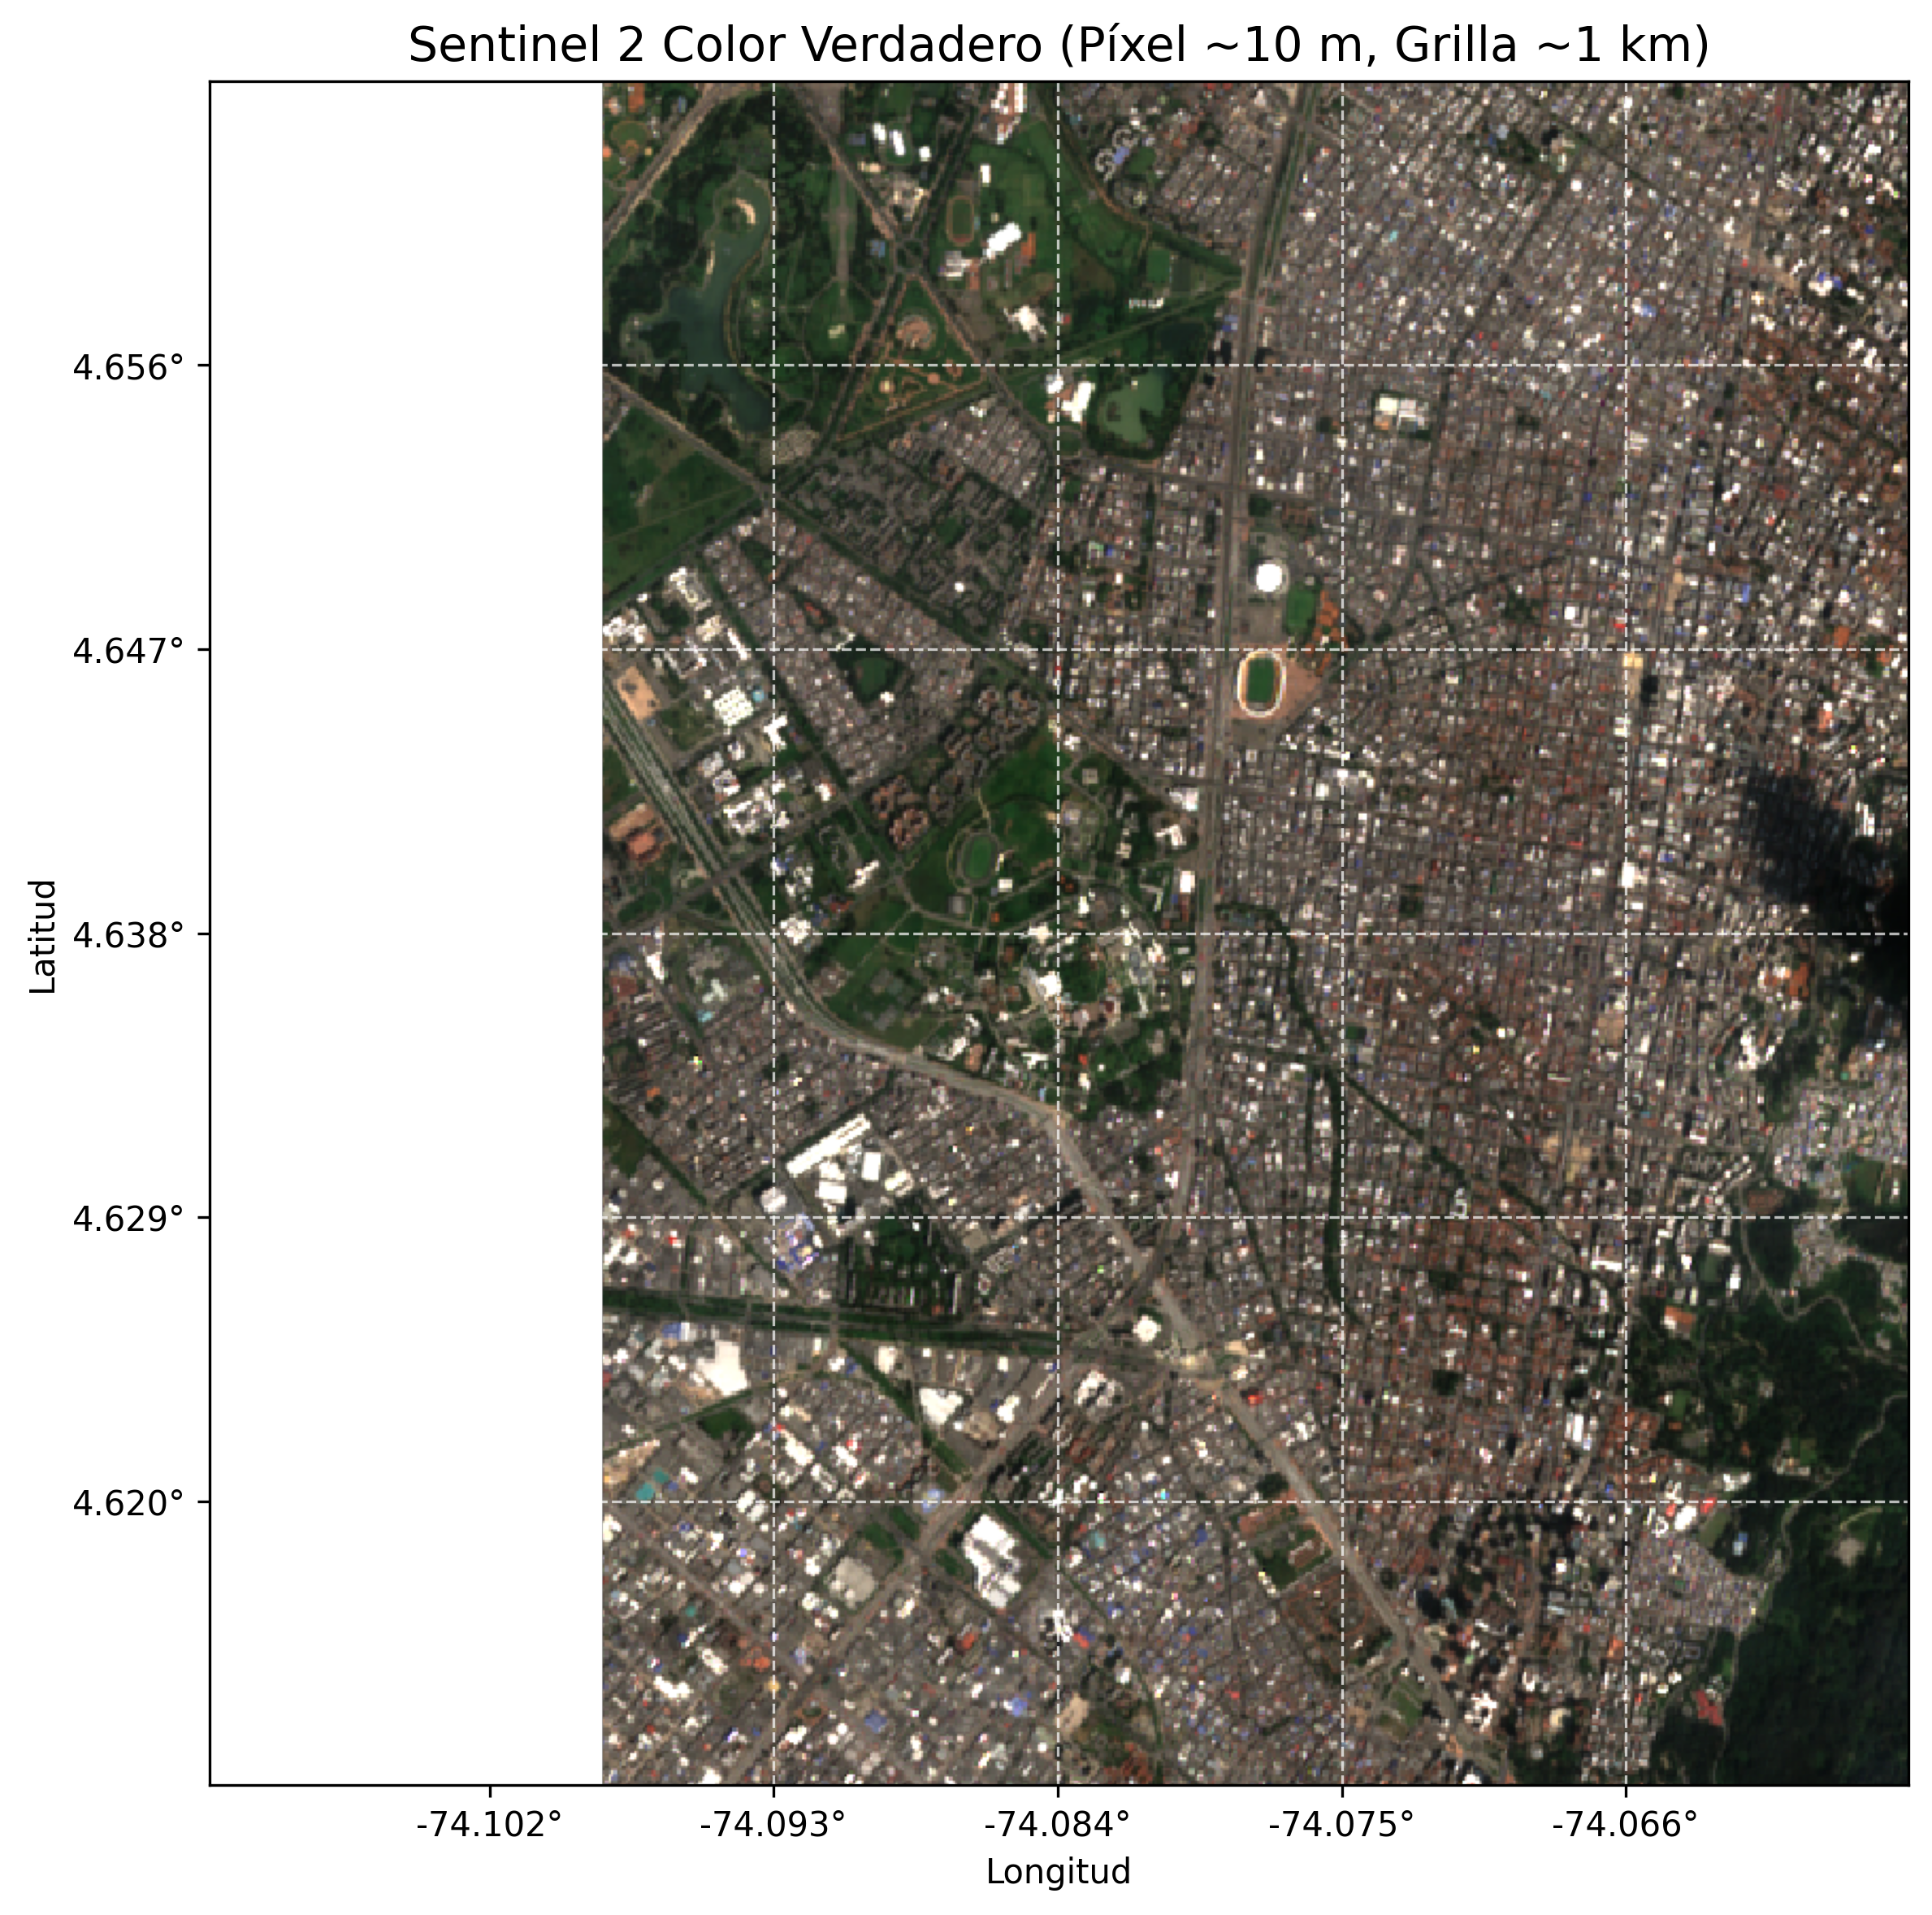
\includegraphics{45-practica_5_clase6_introduccion_sr_gee_files/figure-pdf/fig-python_s2_estatico-output-1.png}

}

\caption{\label{fig-python_s2_estatico}Imagen estática del catálogo
Sentinel-2 en color verdadero.}

\end{figure}%

\subsection{Javascript}

Para ejecutar este código, debes abrir el
\textbf{\href{https://code.earthengine.google.com/}{Code Editor de
Google Earth Engine}} en tu navegador, pegar el siguiente fragmento en
la consola central y hacer clic en \textbf{``Run''}.

\phantomsection\label{js_s2}%
\begin{Shaded}
\begin{Highlighting}[]
\CommentTok{// 1. DEFINICIÓN DEL PUNTO GEOGRÁFICO}
\KeywordTok{var}\NormalTok{ punto\_unal }\OperatorTok{=}\NormalTok{ ee}\OperatorTok{.}\AttributeTok{Geometry}\OperatorTok{.}\FunctionTok{Point}\NormalTok{([}\OperatorTok{{-}}\FloatTok{74.084}\OperatorTok{,} \FloatTok{4.638}\NormalTok{])}\OperatorTok{;}

\CommentTok{// 2. CENTRAR EL VISOR}
\BuiltInTok{Map}\OperatorTok{.}\FunctionTok{centerObject}\NormalTok{(punto\_unal}\OperatorTok{,} \DecValTok{17}\NormalTok{)}\OperatorTok{;}

\CommentTok{// 3. CONSULTA Y FILTRADO DE DATOS}
\KeywordTok{var}\NormalTok{ s2 }\OperatorTok{=}\NormalTok{ ee}\OperatorTok{.}\FunctionTok{ImageCollection}\NormalTok{(}\StringTok{"COPERNICUS/S2\_SR\_HARMONIZED"}\NormalTok{)}
  \OperatorTok{.}\FunctionTok{filterBounds}\NormalTok{(punto\_unal)}
  \OperatorTok{.}\FunctionTok{filterDate}\NormalTok{(}\StringTok{\textquotesingle{}2023{-}01{-}01\textquotesingle{}}\OperatorTok{,} \StringTok{\textquotesingle{}2023{-}12{-}31\textquotesingle{}}\NormalTok{)}
  \OperatorTok{.}\FunctionTok{filter}\NormalTok{(ee}\OperatorTok{.}\AttributeTok{Filter}\OperatorTok{.}\FunctionTok{lt}\NormalTok{(}\StringTok{\textquotesingle{}CLOUDY\_PIXEL\_PERCENTAGE\textquotesingle{}}\OperatorTok{,} \DecValTok{10}\NormalTok{))}
  \OperatorTok{.}\FunctionTok{sort}\NormalTok{(}\StringTok{\textquotesingle{}CLOUDY\_PIXEL\_PERCENTAGE\textquotesingle{}}\NormalTok{)}
  \OperatorTok{.}\FunctionTok{first}\NormalTok{()}\OperatorTok{;}

\CommentTok{// 4. PARÁMETROS DE VISUALIZACIÓN}
\KeywordTok{var}\NormalTok{ visParams }\OperatorTok{=}\NormalTok{ \{}\DataTypeTok{bands}\OperatorTok{:}\NormalTok{ [}\StringTok{\textquotesingle{}B4\textquotesingle{}}\OperatorTok{,} \StringTok{\textquotesingle{}B3\textquotesingle{}}\OperatorTok{,} \StringTok{\textquotesingle{}B2\textquotesingle{}}\NormalTok{]}\OperatorTok{,} \DataTypeTok{min}\OperatorTok{:} \DecValTok{0}\OperatorTok{,} \DataTypeTok{max}\OperatorTok{:} \DecValTok{3000}\NormalTok{\}}\OperatorTok{;}

\CommentTok{// 5. MOSTRAR EN PANTALLA Y EN CONSOLA}
\BuiltInTok{Map}\OperatorTok{.}\FunctionTok{addLayer}\NormalTok{(s2}\OperatorTok{,}\NormalTok{ visParams}\OperatorTok{,} \StringTok{\textquotesingle{}Sentinel 2 {-} UNAL Bogotá\textquotesingle{}}\NormalTok{)}\OperatorTok{;}

\FunctionTok{print}\NormalTok{(}\StringTok{\textquotesingle{}Metadatos de la imagen Sentinel 2:\textquotesingle{}}\OperatorTok{,}\NormalTok{ s2)}\OperatorTok{;}
\FunctionTok{print}\NormalTok{(}\StringTok{\textquotesingle{}ID exacto de la imagen Sentinel 2:\textquotesingle{}}\OperatorTok{,}\NormalTok{ s2}\OperatorTok{.}\FunctionTok{get}\NormalTok{(}\StringTok{\textquotesingle{}system:id\textquotesingle{}}\NormalTok{))}\OperatorTok{;}
\end{Highlighting}
\end{Shaded}

\begin{center}\rule{0.5\linewidth}{0.5pt}\end{center}

\phantomsection\label{js_s2_estatico}%
\begin{Shaded}
\begin{Highlighting}[]
\CommentTok{// ▷ CÓDIGO MAPA ESTÁTICO (THUMBNAIL) EN JAVASCRIPT (Independiente)}

\CommentTok{// 1. DEFINICIÓN DEL PUNTO Y REGIÓN DE INTERÉS}
\KeywordTok{var}\NormalTok{ punto\_unal }\OperatorTok{=}\NormalTok{ ee}\OperatorTok{.}\AttributeTok{Geometry}\OperatorTok{.}\FunctionTok{Point}\NormalTok{([}\OperatorTok{{-}}\FloatTok{74.084}\OperatorTok{,} \FloatTok{4.638}\NormalTok{])}\OperatorTok{;}
\KeywordTok{var}\NormalTok{ region\_interes }\OperatorTok{=}\NormalTok{ punto\_unal}\OperatorTok{.}\FunctionTok{buffer}\NormalTok{(}\DecValTok{3000}\NormalTok{)}\OperatorTok{;} 

\CommentTok{// 2. CONSULTA Y SELECCIÓN DE LA IMAGEN}
\KeywordTok{var}\NormalTok{ s2\_estatica }\OperatorTok{=}\NormalTok{ ee}\OperatorTok{.}\FunctionTok{ImageCollection}\NormalTok{(}\StringTok{"COPERNICUS/S2\_SR\_HARMONIZED"}\NormalTok{)}
  \OperatorTok{.}\FunctionTok{filterBounds}\NormalTok{(punto\_unal)}
  \OperatorTok{.}\FunctionTok{filterDate}\NormalTok{(}\StringTok{\textquotesingle{}2023{-}01{-}01\textquotesingle{}}\OperatorTok{,} \StringTok{\textquotesingle{}2023{-}12{-}31\textquotesingle{}}\NormalTok{)}
  \OperatorTok{.}\FunctionTok{filter}\NormalTok{(ee}\OperatorTok{.}\AttributeTok{Filter}\OperatorTok{.}\FunctionTok{lt}\NormalTok{(}\StringTok{\textquotesingle{}CLOUDY\_PIXEL\_PERCENTAGE\textquotesingle{}}\OperatorTok{,} \DecValTok{10}\NormalTok{))}
  \OperatorTok{.}\FunctionTok{sort}\NormalTok{(}\StringTok{\textquotesingle{}CLOUDY\_PIXEL\_PERCENTAGE\textquotesingle{}}\NormalTok{)}
  \OperatorTok{.}\FunctionTok{first}\NormalTok{()}\OperatorTok{;}

\CommentTok{// 3. PARÁMETROS DE VISUALIZACIÓN}
\KeywordTok{var}\NormalTok{ visParamsEstatica }\OperatorTok{=}\NormalTok{ \{}
  \DataTypeTok{bands}\OperatorTok{:}\NormalTok{ [}\StringTok{\textquotesingle{}B4\textquotesingle{}}\OperatorTok{,} \StringTok{\textquotesingle{}B3\textquotesingle{}}\OperatorTok{,} \StringTok{\textquotesingle{}B2\textquotesingle{}}\NormalTok{]}\OperatorTok{,}
  \DataTypeTok{min}\OperatorTok{:} \DecValTok{0}\OperatorTok{,}
  \DataTypeTok{max}\OperatorTok{:} \DecValTok{3000}\OperatorTok{,}
  \DataTypeTok{dimensions}\OperatorTok{:} \DecValTok{800}\OperatorTok{,}
  \DataTypeTok{region}\OperatorTok{:}\NormalTok{ region\_interes}
\NormalTok{\}}\OperatorTok{;}

\CommentTok{// 4. MOSTRAR EN CONSOLA LA URL Y EL THUMBNAIL}
\FunctionTok{print}\NormalTok{(}\StringTok{\textquotesingle{}URL de la imagen PNG:\textquotesingle{}}\OperatorTok{,}\NormalTok{ s2\_estatica}\OperatorTok{.}\FunctionTok{getThumbURL}\NormalTok{(visParamsEstatica))}\OperatorTok{;}

\KeywordTok{var}\NormalTok{ miniatura }\OperatorTok{=}\NormalTok{ ui}\OperatorTok{.}\FunctionTok{Thumbnail}\NormalTok{(\{}
  \DataTypeTok{image}\OperatorTok{:}\NormalTok{ s2\_estatica}\OperatorTok{,}
  \DataTypeTok{params}\OperatorTok{:}\NormalTok{ visParamsEstatica}\OperatorTok{,}
  \DataTypeTok{style}\OperatorTok{:}\NormalTok{ \{}\DataTypeTok{width}\OperatorTok{:} \StringTok{\textquotesingle{}400px\textquotesingle{}}\OperatorTok{,} \DataTypeTok{height}\OperatorTok{:} \StringTok{\textquotesingle{}400px\textquotesingle{}}\NormalTok{\}}
\NormalTok{\})}\OperatorTok{;}
\FunctionTok{print}\NormalTok{(}\StringTok{\textquotesingle{}Vista previa estática:\textquotesingle{}}\OperatorTok{,}\NormalTok{ miniatura)}\OperatorTok{;}
\end{Highlighting}
\end{Shaded}

\begin{center}\rule{0.5\linewidth}{0.5pt}\end{center}

\subsection{Reto: Cargar imagen en QGIS y ArcGIS
Pro}\label{reto-cargar-imagen-en-qgis-y-arcgis-pro}

Utilizando el mismo patrón que empleamos en la sección de Landsat, tu
misión es llevar esta imagen específica de Sentinel 2 a tus sistemas de
información geográfica de escritorio.

\textbf{Instrucciones:}

\begin{enumerate}
\def\labelenumi{\arabic{enumi}.}
\tightlist
\item
  Ejecuta el código de Python de Sentinel 2 para generar los archivos
  JSON e imprimir en consola el \textbf{Asset ID} exacto de la imagen
  con menor nubosidad.
\item
  Abre \textbf{QGIS}, navega a la pestaña \emph{Load} del plugin de
  Google Earth Engine, y carga la imagen introduciendo el Asset ID y los
  parámetros de visualización (\texttt{B4,B3,B2} y rango \texttt{0} a
  \texttt{3000}).
\item
  Abre \textbf{ArcGIS Pro} y utiliza la herramienta \emph{Add Image to
  Map by Serialized Object} cargando el archivo
  \texttt{sentinel2\_serializado.json}, o usa la herramienta \emph{Add
  Image to Map by Asset ID} usando el identificador crudo.
\item
  \textbf{Reporte:} Toma una captura de pantalla de las herramientas con
  todos los parámetros diligenciados justo antes de ejecutarlas (una
  captura del plugin en QGIS y otra de la herramienta en ArcGIS Pro).
  Reemplaza las rutas del siguiente bloque en tu documento QMD para
  mostrar tus evidencias:
\end{enumerate}

\begin{quote}
\textbf{Reporte visual de Sentinel 2}

\emph{Captura de QGIS (Pestaña Load):}
\texttt{!{[}Mis\ parámetros\ de\ Sentinel\ 2\ en\ QGIS{]}(ruta/a/tu/captura\_qgis\_s2.png)\{fig-align="center"\ width="80\%"\}}

\emph{Captura de ArcGIS Pro (Herramienta utilizada):}
\texttt{!{[}Mis\ parámetros\ de\ Sentinel\ 2\ en\ ArcGIS\ Pro{]}(ruta/a/tu/captura\_arcgis\_s2.png)\{fig-align="center"\ width="80\%"\}}
\end{quote}

\section{Catálogo de datos: Sentinel 1
(SAR)}\label{catuxe1logo-de-datos-sentinel-1-sar}

Imágenes de Radar de Apertura Sintética. A diferencia de los sensores
ópticos, el radar permite obtener datos sin importar la cobertura de
nubes o la iluminación solar.

\begin{longtable}[]{@{}lll@{}}
\toprule\noalign{}
Banda & Resolución & Descripción \\
\midrule\noalign{}
\endhead
\bottomrule\noalign{}
\endlastfoot
VV & 10m & Polarización Vertical-Vertical \\
VH & 10m & Polarización Vertical-Horizontal \\
\end{longtable}

\subsection{Python}

\begin{Shaded}
\begin{Highlighting}[]
\CommentTok{\# \#| eval: false}

\CommentTok{\# Código usando Folium!}

\ImportTok{import}\NormalTok{ ee}
\ImportTok{import}\NormalTok{ folium}
\ImportTok{import}\NormalTok{ datetime}
\ImportTok{import}\NormalTok{ json}

\CommentTok{\# 1. DEFINICIÓN DEL PUNTO GEOGRÁFICO}
\NormalTok{unal\_punto }\OperatorTok{=}\NormalTok{ ee.Geometry.Point([}\OperatorTok{{-}}\FloatTok{74.084}\NormalTok{, }\FloatTok{4.638}\NormalTok{])}

\CommentTok{\# 2. EXPLORAR TODAS LAS OPCIONES Y FILTRAR}
\NormalTok{coleccion\_s1 }\OperatorTok{=}\NormalTok{ (ee.ImageCollection(}\StringTok{"COPERNICUS/S1\_GRD"}\NormalTok{)}
\NormalTok{    .filterBounds(unal\_punto)}
\NormalTok{    .filterDate(}\StringTok{\textquotesingle{}2023{-}01{-}01\textquotesingle{}}\NormalTok{, }\StringTok{\textquotesingle{}2023{-}12{-}31\textquotesingle{}}\NormalTok{)}
\NormalTok{    .}\BuiltInTok{filter}\NormalTok{(ee.Filter.listContains(}\StringTok{\textquotesingle{}transmitterReceiverPolarisation\textquotesingle{}}\NormalTok{, }\StringTok{\textquotesingle{}VV\textquotesingle{}}\NormalTok{)))}

\CommentTok{\# 3. DIAGNÓSTICO: EXTRAER EL TOP 3 DE IMÁGENES}
\NormalTok{ids }\OperatorTok{=}\NormalTok{ coleccion\_s1.aggregate\_array(}\StringTok{\textquotesingle{}system:id\textquotesingle{}}\NormalTok{).getInfo()}
\NormalTok{fechas }\OperatorTok{=}\NormalTok{ coleccion\_s1.aggregate\_array(}\StringTok{\textquotesingle{}system:time\_start\textquotesingle{}}\NormalTok{).getInfo()}

\BuiltInTok{print}\NormalTok{(}\StringTok{"{-}{-}{-} TOP 3 IMÁGENES SENTINEL{-}1 (2023) {-}{-}{-}"}\NormalTok{)}
\ControlFlowTok{for}\NormalTok{ i }\KeywordTok{in} \BuiltInTok{range}\NormalTok{(}\BuiltInTok{min}\NormalTok{(}\DecValTok{3}\NormalTok{, }\BuiltInTok{len}\NormalTok{(ids))):}
\NormalTok{    fecha\_legible }\OperatorTok{=}\NormalTok{ datetime.datetime.fromtimestamp(fechas[i] }\OperatorTok{/} \FloatTok{1000.0}\NormalTok{, datetime.UTC).strftime(}\StringTok{\textquotesingle{}\%Y{-}\%m{-}}\SpecialCharTok{\%d}\StringTok{\textquotesingle{}}\NormalTok{)}
    \BuiltInTok{print}\NormalTok{(}\SpecialStringTok{f"Opción }\SpecialCharTok{\{}\NormalTok{i}\OperatorTok{+}\DecValTok{1}\SpecialCharTok{\}}\SpecialStringTok{ | Fecha: }\SpecialCharTok{\{}\NormalTok{fecha\_legible}\SpecialCharTok{\}}\SpecialStringTok{"}\NormalTok{)}
    \BuiltInTok{print}\NormalTok{(}\SpecialStringTok{f"ID: }\SpecialCharTok{\{}\NormalTok{ids[i]}\SpecialCharTok{\}}\CharTok{\textbackslash{}n}\SpecialStringTok{"}\NormalTok{)}
\BuiltInTok{print}\NormalTok{(}\StringTok{"{-}{-}{-}{-}{-}{-}{-}{-}{-}{-}{-}{-}{-}{-}{-}{-}{-}{-}{-}{-}{-}{-}{-}{-}{-}{-}{-}{-}{-}{-}{-}{-}{-}{-}{-}{-}{-}{-}{-}{-}{-}{-}{-}{-}{-}{-}{-}{-}{-}{-}{-}{-}{-}{-}{-}{-}{-}{-}{-}{-}{-}{-}{-}{-}"}\NormalTok{)}

\CommentTok{\# 4. SELECCIÓN DEFINITIVA DE LA IMAGEN}
\NormalTok{s1 }\OperatorTok{=}\NormalTok{ ee.Image(coleccion\_s1.first())}

\CommentTok{\# 5. EXPORTAR LOS ARCHIVOS JSON (METADATOS Y SERIALIZADO)}
\NormalTok{id\_exacto }\OperatorTok{=}\NormalTok{ s1.get(}\StringTok{\textquotesingle{}system:id\textquotesingle{}}\NormalTok{).getInfo()}
\BuiltInTok{print}\NormalTok{(}\SpecialStringTok{f"}\CharTok{\textbackslash{}n}\SpecialStringTok{ID de la imagen Sentinel 1 seleccionada: }\SpecialCharTok{\{}\NormalTok{id\_exacto}\SpecialCharTok{\}}\SpecialStringTok{"}\NormalTok{)}

\NormalTok{metadatos\_json }\OperatorTok{=}\NormalTok{ s1.getInfo()}
\ControlFlowTok{with} \BuiltInTok{open}\NormalTok{(}\StringTok{\textquotesingle{}metadatos\_sentinel1.json\textquotesingle{}}\NormalTok{, }\StringTok{\textquotesingle{}w\textquotesingle{}}\NormalTok{) }\ImportTok{as}\NormalTok{ archivo:}
\NormalTok{    json.dump(metadatos\_json, archivo, indent}\OperatorTok{=}\DecValTok{4}\NormalTok{)}

\NormalTok{s1\_limpia }\OperatorTok{=}\NormalTok{ ee.Image(id\_exacto)}
\NormalTok{texto\_json\_serializado }\OperatorTok{=}\NormalTok{ s1\_limpia.serialize()}
\ControlFlowTok{with} \BuiltInTok{open}\NormalTok{(}\StringTok{\textquotesingle{}sentinel1\_serializado.json\textquotesingle{}}\NormalTok{, }\StringTok{\textquotesingle{}w\textquotesingle{}}\NormalTok{) }\ImportTok{as}\NormalTok{ archivo:}
\NormalTok{    json.dump(texto\_json\_serializado, archivo)}

\CommentTok{\# 6. PARÁMETROS DE VISUALIZACIÓN}
\NormalTok{vis\_params }\OperatorTok{=}\NormalTok{ \{}\StringTok{\textquotesingle{}bands\textquotesingle{}}\NormalTok{: [}\StringTok{\textquotesingle{}VV\textquotesingle{}}\NormalTok{], }\StringTok{\textquotesingle{}min\textquotesingle{}}\NormalTok{: }\OperatorTok{{-}}\DecValTok{20}\NormalTok{, }\StringTok{\textquotesingle{}max\textquotesingle{}}\NormalTok{: }\DecValTok{0}\NormalTok{\}}
\NormalTok{map\_id\_dict }\OperatorTok{=}\NormalTok{ ee.Image(s1).getMapId(vis\_params)}

\CommentTok{\# 7. MENSAJE FINAL}
\NormalTok{fecha\_capa\_ms }\OperatorTok{=}\NormalTok{ s1.get(}\StringTok{\textquotesingle{}system:time\_start\textquotesingle{}}\NormalTok{).getInfo()}
\NormalTok{fecha\_capa }\OperatorTok{=}\NormalTok{ datetime.datetime.fromtimestamp(fecha\_capa\_ms }\OperatorTok{/} \FloatTok{1000.0}\NormalTok{, datetime.UTC).strftime(}\StringTok{\textquotesingle{}\%Y{-}\%m{-}}\SpecialCharTok{\%d}\StringTok{\textquotesingle{}}\NormalTok{)}

\BuiltInTok{print}\NormalTok{(}\StringTok{"}\CharTok{\textbackslash{}n}\StringTok{✅ MAPA GENERADO CON ÉXITO"}\NormalTok{)}
\BuiltInTok{print}\NormalTok{(}\SpecialStringTok{f"Capa desplegada : Sentinel 1 VV {-} }\SpecialCharTok{\{}\NormalTok{fecha\_capa}\SpecialCharTok{\}}\SpecialStringTok{"}\NormalTok{)}
\BuiltInTok{print}\NormalTok{(}\StringTok{"{-}{-}{-}{-}{-}{-}{-}{-}{-}{-}{-}{-}{-}{-}{-}{-}{-}{-}{-}{-}{-}{-}{-}{-}{-}{-}{-}{-}{-}{-}{-}{-}{-}{-}{-}{-}{-}{-}{-}{-}{-}{-}{-}{-}{-}{-}{-}{-}{-}{-}{-}{-}{-}{-}{-}{-}{-}{-}{-}{-}{-}{-}{-}{-}"}\NormalTok{)}

\CommentTok{\# 8. CONFIGURACIÓN DEL MAPA BASE (Folium)}
\NormalTok{Map\_s1 }\OperatorTok{=}\NormalTok{ folium.Map(location}\OperatorTok{=}\NormalTok{[}\FloatTok{4.638}\NormalTok{, }\OperatorTok{{-}}\FloatTok{74.084}\NormalTok{], zoom\_start}\OperatorTok{=}\DecValTok{17}\NormalTok{)}

\CommentTok{\# 9. AGREGAR LA IMAGEN AL VISOR}
\NormalTok{folium.TileLayer(}
\NormalTok{    tiles}\OperatorTok{=}\NormalTok{map\_id\_dict[}\StringTok{\textquotesingle{}tile\_fetcher\textquotesingle{}}\NormalTok{].url\_format,}
\NormalTok{    attr}\OperatorTok{=}\StringTok{\textquotesingle{}Google Earth Engine\textquotesingle{}}\NormalTok{,}
\NormalTok{    overlay}\OperatorTok{=}\VariableTok{True}\NormalTok{,}
\NormalTok{    name}\OperatorTok{=}\SpecialStringTok{f\textquotesingle{}Sentinel 1 VV {-} }\SpecialCharTok{\{}\NormalTok{fecha\_capa}\SpecialCharTok{\}}\SpecialStringTok{\textquotesingle{}}
\NormalTok{).add\_to(Map\_s1)}

\NormalTok{folium.LayerControl().add\_to(Map\_s1)}

\CommentTok{\# 10. VISUALIZACIÓN DEL RESULTADO}
\CommentTok{\# Map\_s1}
\CommentTok{\#from IPython.display import display, HTML}
\CommentTok{\#display(HTML(Map\_s1.\_repr\_html\_()))}

\ImportTok{from}\NormalTok{ IPython.display }\ImportTok{import}\NormalTok{ IFrame}

\CommentTok{\# Guardamos el mapa aislado en tu carpeta de trabajo}
\NormalTok{Map\_s1.save(}\StringTok{"mapas/map\_s1.html"}\NormalTok{)}

\CommentTok{\# Lo incrustamos en el documento Quarto como una página web independiente}
\NormalTok{display(IFrame(src}\OperatorTok{=}\StringTok{"mapas/map\_s1.html"}\NormalTok{, width}\OperatorTok{=}\StringTok{"100\%"}\NormalTok{, height}\OperatorTok{=}\StringTok{"500px"}\NormalTok{))}
\end{Highlighting}
\end{Shaded}

\begin{verbatim}
--- TOP 3 IMÁGENES SENTINEL-1 (2023) ---
Opción 1 | Fecha: 2023-01-08
ID: COPERNICUS/S1_GRD/S1A_IW_GRDH_1SDV_20230108T104325_20230108T104350_046691_0598C2_C3AE

Opción 2 | Fecha: 2023-01-20
ID: COPERNICUS/S1_GRD/S1A_IW_GRDH_1SDV_20230120T104324_20230120T104349_046866_059EAB_3CB6

Opción 3 | Fecha: 2023-02-01
ID: COPERNICUS/S1_GRD/S1A_IW_GRDH_1SDV_20230201T104324_20230201T104349_047041_05A488_DAC8

----------------------------------------------------------------

ID de la imagen Sentinel 1 seleccionada: COPERNICUS/S1_GRD/S1A_IW_GRDH_1SDV_20230108T104325_20230108T104350_046691_0598C2_C3AE

✅ MAPA GENERADO CON ÉXITO
Capa desplegada : Sentinel 1 VV - 2023-01-08
----------------------------------------------------------------
\end{verbatim}

\phantomsection\label{python_s1}
\begin{verbatim}
<IPython.lib.display.IFrame at 0x7ac2a3100da0>
\end{verbatim}

\begin{center}\rule{0.5\linewidth}{0.5pt}\end{center}

\begin{Shaded}
\begin{Highlighting}[]
\CommentTok{\# \#| eval: false}

\CommentTok{\# ▷ CÓDIGO MAPA ESTÁTICO (PNG) PARA FOLIUM/GENERAL (Independiente)}
\ImportTok{import}\NormalTok{ ee}
\ImportTok{import}\NormalTok{ requests}
\ImportTok{import}\NormalTok{ matplotlib.pyplot }\ImportTok{as}\NormalTok{ plt}
\ImportTok{from}\NormalTok{ PIL }\ImportTok{import}\NormalTok{ Image}
\ImportTok{from}\NormalTok{ io }\ImportTok{import}\NormalTok{ BytesIO}

\CommentTok{\# 1. DEFINICIÓN DEL PUNTO GEOGRÁFICO Y REGIÓN DE INTERÉS}
\NormalTok{lon\_centro, lat\_centro }\OperatorTok{=} \OperatorTok{{-}}\FloatTok{74.084}\NormalTok{, }\FloatTok{4.638}
\NormalTok{unal\_punto }\OperatorTok{=}\NormalTok{ ee.Geometry.Point([lon\_centro, lat\_centro])}
\NormalTok{region\_interes }\OperatorTok{=}\NormalTok{ unal\_punto.}\BuiltInTok{buffer}\NormalTok{(}\DecValTok{3000}\NormalTok{)}

\CommentTok{\# 2. CONSULTA Y SELECCIÓN DE LA IMAGEN}
\NormalTok{s1\_estatica }\OperatorTok{=}\NormalTok{ ee.Image(ee.ImageCollection(}\StringTok{"COPERNICUS/S1\_GRD"}\NormalTok{)}
\NormalTok{    .filterBounds(unal\_punto)}
\NormalTok{    .filterDate(}\StringTok{\textquotesingle{}2023{-}01{-}01\textquotesingle{}}\NormalTok{, }\StringTok{\textquotesingle{}2023{-}12{-}31\textquotesingle{}}\NormalTok{)}
\NormalTok{    .}\BuiltInTok{filter}\NormalTok{(ee.Filter.listContains(}\StringTok{\textquotesingle{}transmitterReceiverPolarisation\textquotesingle{}}\NormalTok{, }\StringTok{\textquotesingle{}VV\textquotesingle{}}\NormalTok{))}
\NormalTok{    .first())}

\CommentTok{\# 3. OBTENER LA URL DEL THUMBNAIL (PNG) DESDE GOOGLE EARTH ENGINE}
\NormalTok{url\_img }\OperatorTok{=}\NormalTok{ s1\_estatica.getThumbURL(\{}
    \StringTok{\textquotesingle{}bands\textquotesingle{}}\NormalTok{: [}\StringTok{\textquotesingle{}VV\textquotesingle{}}\NormalTok{],}
    \StringTok{\textquotesingle{}min\textquotesingle{}}\NormalTok{: }\OperatorTok{{-}}\DecValTok{20}\NormalTok{,}
    \StringTok{\textquotesingle{}max\textquotesingle{}}\NormalTok{: }\DecValTok{0}\NormalTok{,}
    \StringTok{\textquotesingle{}dimensions\textquotesingle{}}\NormalTok{: }\DecValTok{800}\NormalTok{,}
    \StringTok{\textquotesingle{}region\textquotesingle{}}\NormalTok{: region\_interes}
\NormalTok{\})}

\CommentTok{\# 4. DESCARGAR Y DIBUJAR LA IMAGEN CON MATPLOTLIB (Grilla y Coordenadas)}
\NormalTok{respuesta }\OperatorTok{=}\NormalTok{ requests.get(url\_img)}
\NormalTok{imagen\_png }\OperatorTok{=}\NormalTok{ Image.}\BuiltInTok{open}\NormalTok{(BytesIO(respuesta.content))}

\CommentTok{\# Obtenemos las coordenadas límite para georreferenciar la imagen PNG}
\NormalTok{coords }\OperatorTok{=}\NormalTok{ region\_interes.bounds().coordinates().get(}\DecValTok{0}\NormalTok{).getInfo()}
\NormalTok{xmin, ymin }\OperatorTok{=}\NormalTok{ coords[}\DecValTok{0}\NormalTok{][}\DecValTok{0}\NormalTok{], coords[}\DecValTok{0}\NormalTok{][}\DecValTok{1}\NormalTok{]}
\NormalTok{xmax, ymax }\OperatorTok{=}\NormalTok{ coords[}\DecValTok{2}\NormalTok{][}\DecValTok{0}\NormalTok{], coords[}\DecValTok{2}\NormalTok{][}\DecValTok{1}\NormalTok{]}

\NormalTok{fig, ax }\OperatorTok{=}\NormalTok{ plt.subplots(figsize}\OperatorTok{=}\NormalTok{(}\DecValTok{8}\NormalTok{, }\DecValTok{8}\NormalTok{))}

\CommentTok{\# Mapeamos los píxeles a grados}
\NormalTok{ax.imshow(imagen\_png, cmap}\OperatorTok{=}\StringTok{\textquotesingle{}gray\textquotesingle{}}\NormalTok{, extent}\OperatorTok{=}\NormalTok{[xmin, xmax, ymin, ymax])}

\CommentTok{\# Grilla de 1 km. (1 grado ≈ 111 km {-}\textgreater{} 1 km ≈ 0.009 grados)}
\NormalTok{paso\_1km }\OperatorTok{=} \FloatTok{0.009} 

\NormalTok{x\_ticks }\OperatorTok{=}\NormalTok{ [lon\_centro }\OperatorTok{+}\NormalTok{ (i }\OperatorTok{*}\NormalTok{ paso\_1km) }\ControlFlowTok{for}\NormalTok{ i }\KeywordTok{in} \BuiltInTok{range}\NormalTok{(}\OperatorTok{{-}}\DecValTok{4}\NormalTok{, }\DecValTok{5}\NormalTok{)]}
\NormalTok{y\_ticks }\OperatorTok{=}\NormalTok{ [lat\_centro }\OperatorTok{+}\NormalTok{ (i }\OperatorTok{*}\NormalTok{ paso\_1km) }\ControlFlowTok{for}\NormalTok{ i }\KeywordTok{in} \BuiltInTok{range}\NormalTok{(}\OperatorTok{{-}}\DecValTok{4}\NormalTok{, }\DecValTok{5}\NormalTok{)]}

\NormalTok{x\_ticks }\OperatorTok{=}\NormalTok{ [x }\ControlFlowTok{for}\NormalTok{ x }\KeywordTok{in}\NormalTok{ x\_ticks }\ControlFlowTok{if}\NormalTok{ xmin }\OperatorTok{\textless{}=}\NormalTok{ x }\OperatorTok{\textless{}=}\NormalTok{ xmax]}
\NormalTok{y\_ticks }\OperatorTok{=}\NormalTok{ [y }\ControlFlowTok{for}\NormalTok{ y }\KeywordTok{in}\NormalTok{ y\_ticks }\ControlFlowTok{if}\NormalTok{ ymin }\OperatorTok{\textless{}=}\NormalTok{ y }\OperatorTok{\textless{}=}\NormalTok{ ymax]}

\NormalTok{ax.set\_xticks(x\_ticks)}
\NormalTok{ax.set\_yticks(y\_ticks)}
\NormalTok{ax.set\_xticklabels([}\SpecialStringTok{f"}\SpecialCharTok{\{}\NormalTok{x}\SpecialCharTok{:.3f\}}\SpecialStringTok{°"} \ControlFlowTok{for}\NormalTok{ x }\KeywordTok{in}\NormalTok{ x\_ticks])}
\NormalTok{ax.set\_yticklabels([}\SpecialStringTok{f"}\SpecialCharTok{\{}\NormalTok{y}\SpecialCharTok{:.3f\}}\SpecialStringTok{°"} \ControlFlowTok{for}\NormalTok{ y }\KeywordTok{in}\NormalTok{ y\_ticks])}

\NormalTok{ax.grid(color}\OperatorTok{=}\StringTok{\textquotesingle{}white\textquotesingle{}}\NormalTok{, linestyle}\OperatorTok{=}\StringTok{\textquotesingle{}{-}{-}\textquotesingle{}}\NormalTok{, linewidth}\OperatorTok{=}\FloatTok{0.8}\NormalTok{, alpha}\OperatorTok{=}\FloatTok{0.7}\NormalTok{)}
\NormalTok{ax.set\_title(}\StringTok{\textquotesingle{}Sentinel 1 VV (Píxel \textasciitilde{}10 m, Grilla \textasciitilde{}1 km)\textquotesingle{}}\NormalTok{, fontsize}\OperatorTok{=}\DecValTok{14}\NormalTok{)}
\NormalTok{ax.set\_xlabel(}\StringTok{\textquotesingle{}Longitud\textquotesingle{}}\NormalTok{)}
\NormalTok{ax.set\_ylabel(}\StringTok{\textquotesingle{}Latitud\textquotesingle{}}\NormalTok{)}

\NormalTok{plt.tight\_layout()}
\NormalTok{plt.show()}
\end{Highlighting}
\end{Shaded}

\begin{figure}[H]

\centering{

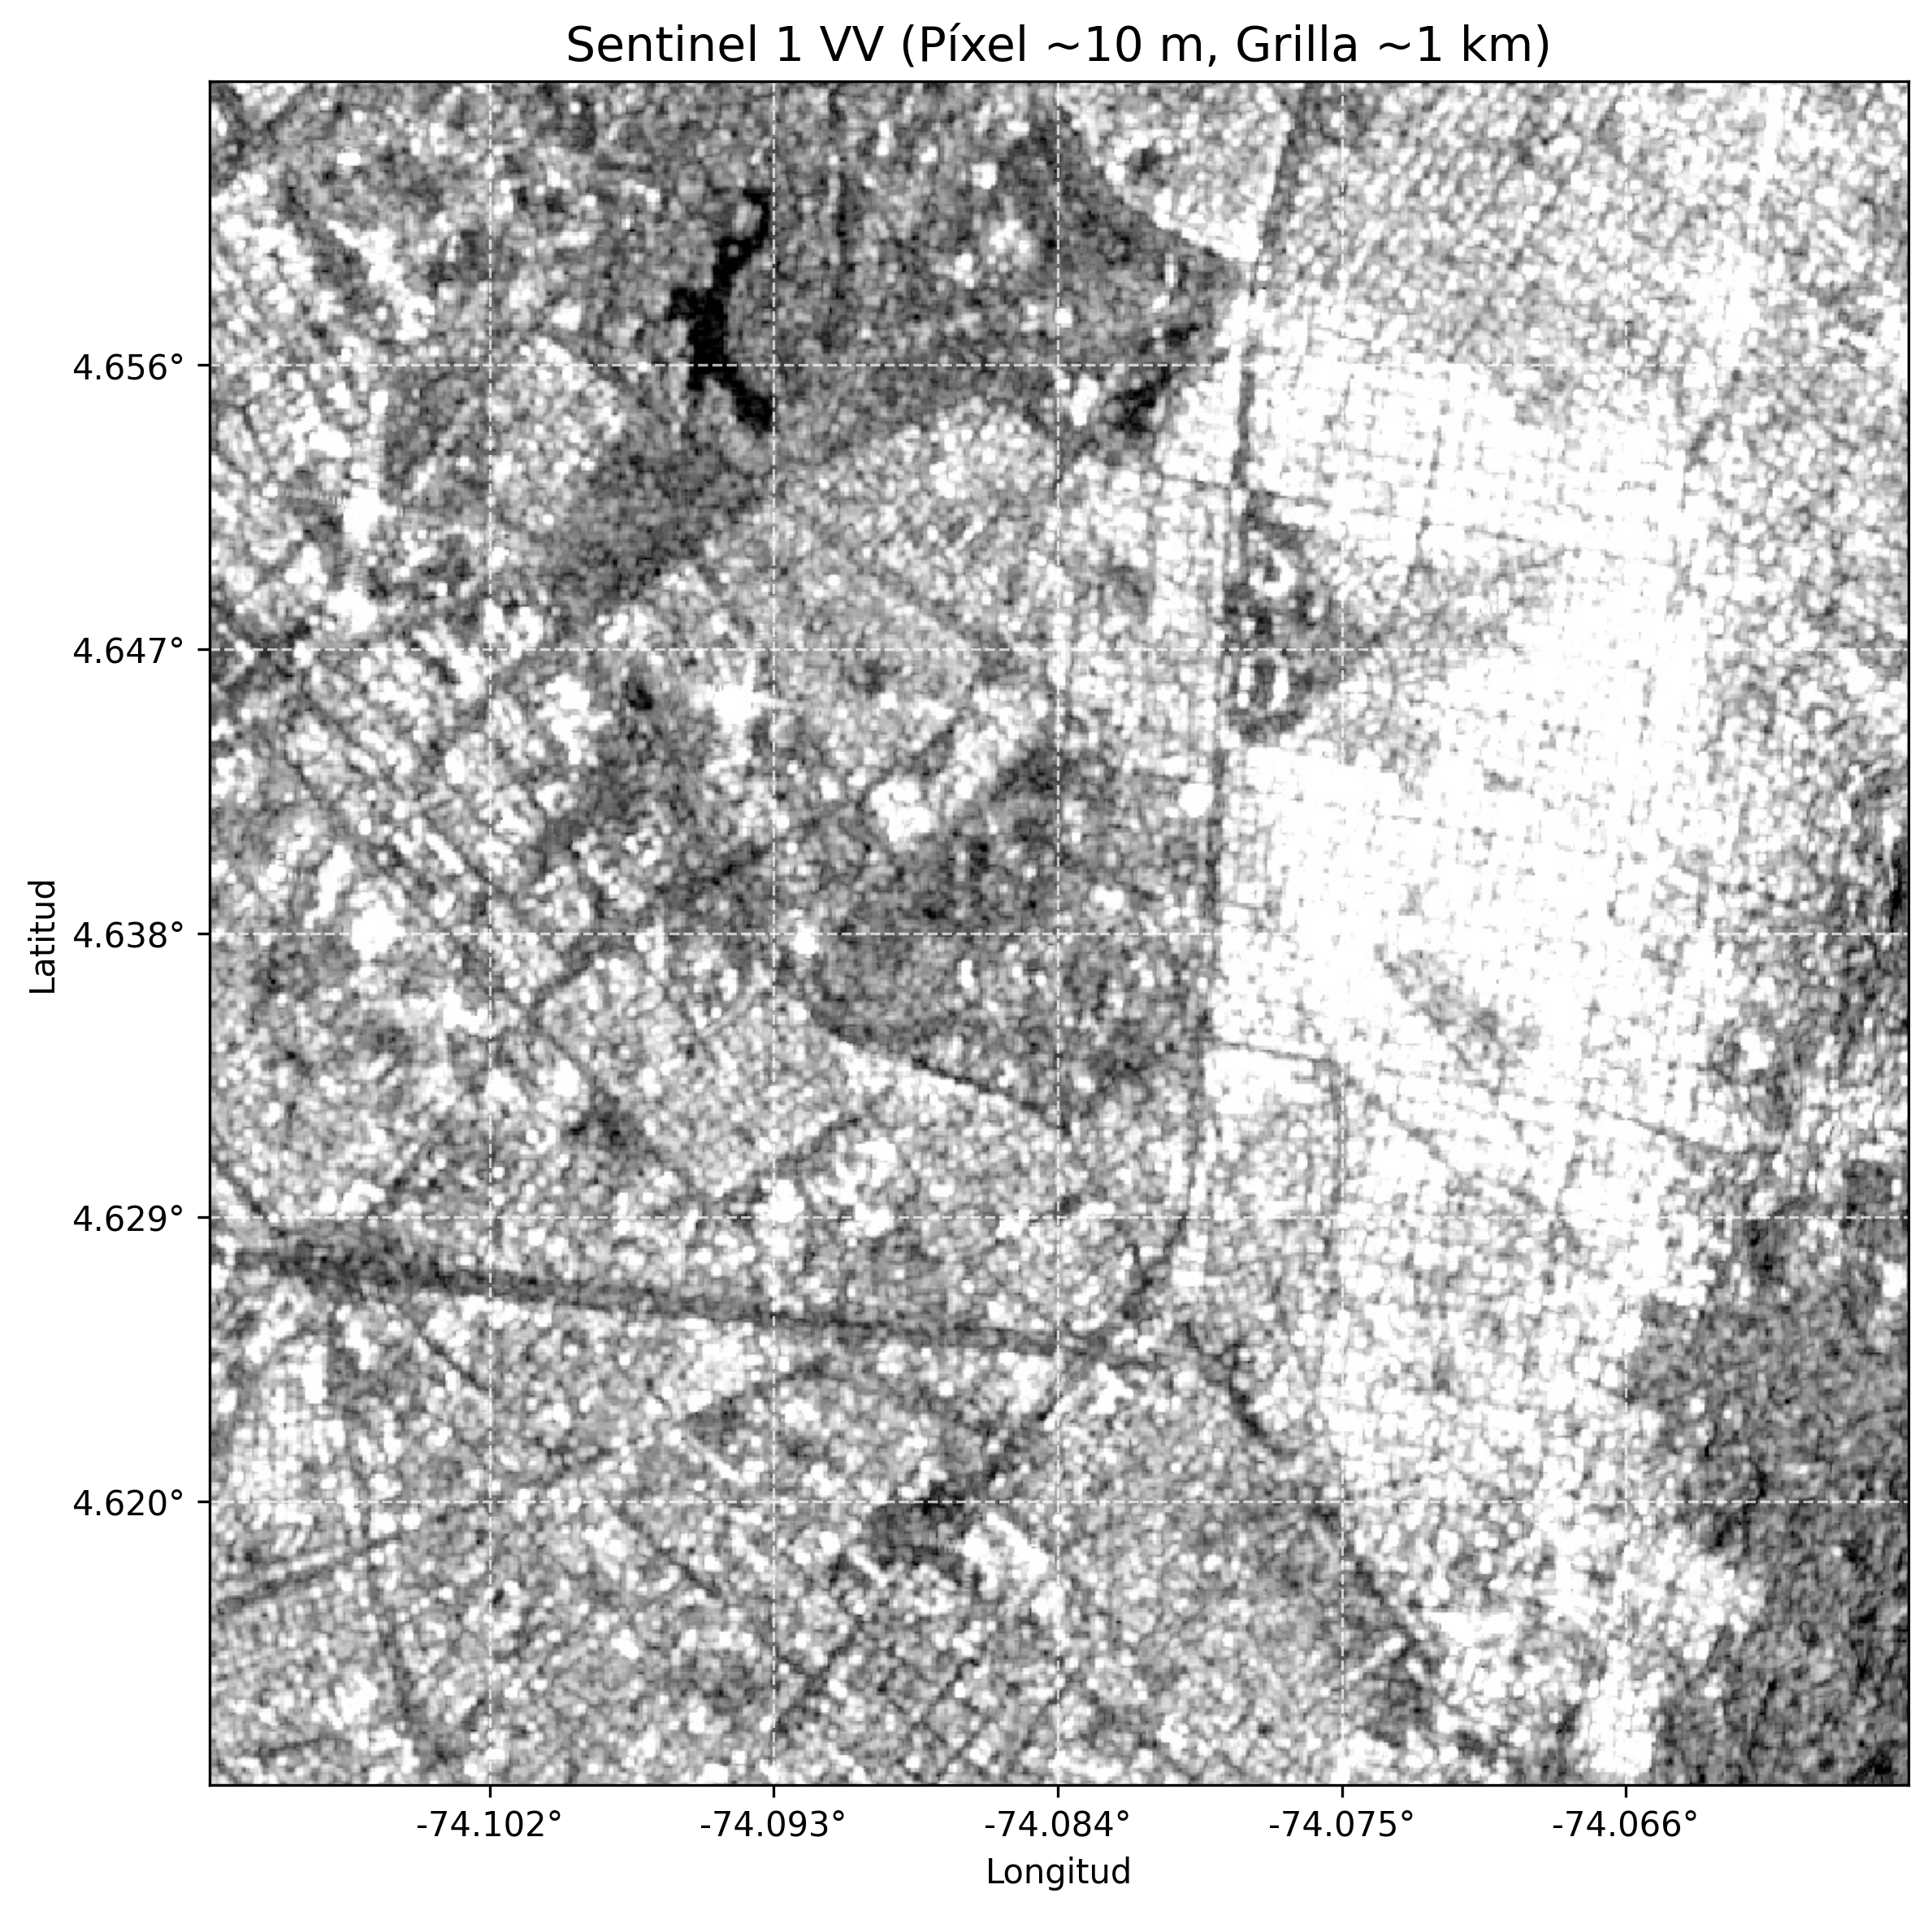
\includegraphics{45-practica_5_clase6_introduccion_sr_gee_files/figure-pdf/fig-python_s1_estatico-output-1.png}

}

\caption{\label{fig-python_s1_estatico}Imagen estática del catálogo
Sentinel-1 (Radar SAR) en polarización VV con grilla de referencia.}

\end{figure}%

\subsection{Javascript}

Para ejecutar este código, debes abrir el
\textbf{\href{https://code.earthengine.google.com/}{Code Editor de
Google Earth Engine}} en tu navegador, pegar el siguiente fragmento en
la consola central y hacer clic en \textbf{``Run''}.

\phantomsection\label{js_s1}%
\begin{Shaded}
\begin{Highlighting}[]
\CommentTok{// 1. DEFINICIÓN DEL PUNTO GEOGRÁFICO}
\KeywordTok{var}\NormalTok{ punto\_unal }\OperatorTok{=}\NormalTok{ ee}\OperatorTok{.}\AttributeTok{Geometry}\OperatorTok{.}\FunctionTok{Point}\NormalTok{([}\OperatorTok{{-}}\FloatTok{74.084}\OperatorTok{,} \FloatTok{4.638}\NormalTok{])}\OperatorTok{;}

\CommentTok{// 2. CENTRAR EL VISOR}
\BuiltInTok{Map}\OperatorTok{.}\FunctionTok{centerObject}\NormalTok{(punto\_unal}\OperatorTok{,} \DecValTok{17}\NormalTok{)}\OperatorTok{;}

\CommentTok{// 3. CONSULTA Y FILTRADO DE DATOS}
\KeywordTok{var}\NormalTok{ s1 }\OperatorTok{=}\NormalTok{ ee}\OperatorTok{.}\FunctionTok{ImageCollection}\NormalTok{(}\StringTok{"COPERNICUS/S1\_GRD"}\NormalTok{)}
  \OperatorTok{.}\FunctionTok{filterBounds}\NormalTok{(punto\_unal)}
  \OperatorTok{.}\FunctionTok{filterDate}\NormalTok{(}\StringTok{\textquotesingle{}2023{-}01{-}01\textquotesingle{}}\OperatorTok{,} \StringTok{\textquotesingle{}2023{-}12{-}31\textquotesingle{}}\NormalTok{)}
  \OperatorTok{.}\FunctionTok{filter}\NormalTok{(ee}\OperatorTok{.}\AttributeTok{Filter}\OperatorTok{.}\FunctionTok{listContains}\NormalTok{(}\StringTok{\textquotesingle{}transmitterReceiverPolarisation\textquotesingle{}}\OperatorTok{,} \StringTok{\textquotesingle{}VV\textquotesingle{}}\NormalTok{))}
  \OperatorTok{.}\FunctionTok{first}\NormalTok{()}\OperatorTok{;}

\CommentTok{// 4. PARÁMETROS DE VISUALIZACIÓN}
\KeywordTok{var}\NormalTok{ visParams }\OperatorTok{=}\NormalTok{ \{}\DataTypeTok{bands}\OperatorTok{:}\NormalTok{ [}\StringTok{\textquotesingle{}VV\textquotesingle{}}\NormalTok{]}\OperatorTok{,} \DataTypeTok{min}\OperatorTok{:} \OperatorTok{{-}}\DecValTok{20}\OperatorTok{,} \DataTypeTok{max}\OperatorTok{:} \DecValTok{0}\NormalTok{\}}\OperatorTok{;}

\CommentTok{// 5. MOSTRAR EN PANTALLA Y EN CONSOLA}
\BuiltInTok{Map}\OperatorTok{.}\FunctionTok{addLayer}\NormalTok{(s1}\OperatorTok{,}\NormalTok{ visParams}\OperatorTok{,} \StringTok{\textquotesingle{}Sentinel 1 VV {-} UNAL Bogotá\textquotesingle{}}\NormalTok{)}\OperatorTok{;}

\FunctionTok{print}\NormalTok{(}\StringTok{\textquotesingle{}Metadatos de la imagen Sentinel 1:\textquotesingle{}}\OperatorTok{,}\NormalTok{ s1)}\OperatorTok{;}
\FunctionTok{print}\NormalTok{(}\StringTok{\textquotesingle{}ID exacto de la imagen Sentinel 1:\textquotesingle{}}\OperatorTok{,}\NormalTok{ s1}\OperatorTok{.}\FunctionTok{get}\NormalTok{(}\StringTok{\textquotesingle{}system:id\textquotesingle{}}\NormalTok{))}\OperatorTok{;}
\end{Highlighting}
\end{Shaded}

\begin{center}\rule{0.5\linewidth}{0.5pt}\end{center}

\phantomsection\label{js_s1_estatico}%
\begin{Shaded}
\begin{Highlighting}[]
\CommentTok{// ▷ CÓDIGO MAPA ESTÁTICO (THUMBNAIL) EN JAVASCRIPT (Independiente)}

\CommentTok{// 1. DEFINICIÓN DEL PUNTO Y REGIÓN DE INTERÉS}
\KeywordTok{var}\NormalTok{ punto\_unal }\OperatorTok{=}\NormalTok{ ee}\OperatorTok{.}\AttributeTok{Geometry}\OperatorTok{.}\FunctionTok{Point}\NormalTok{([}\OperatorTok{{-}}\FloatTok{74.084}\OperatorTok{,} \FloatTok{4.638}\NormalTok{])}\OperatorTok{;}
\KeywordTok{var}\NormalTok{ region\_interes }\OperatorTok{=}\NormalTok{ punto\_unal}\OperatorTok{.}\FunctionTok{buffer}\NormalTok{(}\DecValTok{3000}\NormalTok{)}\OperatorTok{;} 

\CommentTok{// 2. CONSULTA Y SELECCIÓN DE LA IMAGEN}
\KeywordTok{var}\NormalTok{ s1\_estatica }\OperatorTok{=}\NormalTok{ ee}\OperatorTok{.}\FunctionTok{ImageCollection}\NormalTok{(}\StringTok{"COPERNICUS/S1\_GRD"}\NormalTok{)}
  \OperatorTok{.}\FunctionTok{filterBounds}\NormalTok{(punto\_unal)}
  \OperatorTok{.}\FunctionTok{filterDate}\NormalTok{(}\StringTok{\textquotesingle{}2023{-}01{-}01\textquotesingle{}}\OperatorTok{,} \StringTok{\textquotesingle{}2023{-}12{-}31\textquotesingle{}}\NormalTok{)}
  \OperatorTok{.}\FunctionTok{filter}\NormalTok{(ee}\OperatorTok{.}\AttributeTok{Filter}\OperatorTok{.}\FunctionTok{listContains}\NormalTok{(}\StringTok{\textquotesingle{}transmitterReceiverPolarisation\textquotesingle{}}\OperatorTok{,} \StringTok{\textquotesingle{}VV\textquotesingle{}}\NormalTok{))}
  \OperatorTok{.}\FunctionTok{first}\NormalTok{()}\OperatorTok{;}

\CommentTok{// 3. PARÁMETROS DE VISUALIZACIÓN}
\KeywordTok{var}\NormalTok{ visParamsEstatica }\OperatorTok{=}\NormalTok{ \{}
  \DataTypeTok{bands}\OperatorTok{:}\NormalTok{ [}\StringTok{\textquotesingle{}VV\textquotesingle{}}\NormalTok{]}\OperatorTok{,}
  \DataTypeTok{min}\OperatorTok{:} \OperatorTok{{-}}\DecValTok{20}\OperatorTok{,}
  \DataTypeTok{max}\OperatorTok{:} \DecValTok{0}\OperatorTok{,}
  \DataTypeTok{dimensions}\OperatorTok{:} \DecValTok{800}\OperatorTok{,}
  \DataTypeTok{region}\OperatorTok{:}\NormalTok{ region\_interes}
\NormalTok{\}}\OperatorTok{;}

\CommentTok{// 4. MOSTRAR EN CONSOLA LA URL Y EL THUMBNAIL}
\FunctionTok{print}\NormalTok{(}\StringTok{\textquotesingle{}URL de la imagen PNG:\textquotesingle{}}\OperatorTok{,}\NormalTok{ s1\_estatica}\OperatorTok{.}\FunctionTok{getThumbURL}\NormalTok{(visParamsEstatica))}\OperatorTok{;}

\KeywordTok{var}\NormalTok{ miniatura }\OperatorTok{=}\NormalTok{ ui}\OperatorTok{.}\FunctionTok{Thumbnail}\NormalTok{(\{}
  \DataTypeTok{image}\OperatorTok{:}\NormalTok{ s1\_estatica}\OperatorTok{,}
  \DataTypeTok{params}\OperatorTok{:}\NormalTok{ visParamsEstatica}\OperatorTok{,}
  \DataTypeTok{style}\OperatorTok{:}\NormalTok{ \{}\DataTypeTok{width}\OperatorTok{:} \StringTok{\textquotesingle{}400px\textquotesingle{}}\OperatorTok{,} \DataTypeTok{height}\OperatorTok{:} \StringTok{\textquotesingle{}400px\textquotesingle{}}\NormalTok{\}}
\NormalTok{\})}\OperatorTok{;}
\FunctionTok{print}\NormalTok{(}\StringTok{\textquotesingle{}Vista previa estática:\textquotesingle{}}\OperatorTok{,}\NormalTok{ miniatura)}\OperatorTok{;}
\end{Highlighting}
\end{Shaded}

\begin{center}\rule{0.5\linewidth}{0.5pt}\end{center}

\subsection{Reto: Cargar imagen en QGIS y ArcGIS
Pro}\label{reto-cargar-imagen-en-qgis-y-arcgis-pro-1}

Utilice el archivo \texttt{sentinel1\_serializado.json} o el Asset ID
generado para cargar la imagen de radar en las plataformas de
escritorio.

\textbf{Instrucciones:}

\begin{enumerate}
\def\labelenumi{\arabic{enumi}.}
\tightlist
\item
  Ejecute el código de Python de Sentinel 1 para generar los archivos
  JSON e imprimir en consola el Asset ID.
\item
  En \textbf{QGIS}, utilice la pestaña \emph{Load} del plugin de Google
  Earth Engine. Introduzca el Asset ID y los parámetros de visualización
  (Banda \texttt{VV} y rango \texttt{-20} a \texttt{0}).
\item
  En \textbf{ArcGIS Pro}, utilice la herramienta \emph{Add Image to Map
  by Serialized Object} o \emph{Add Image to Map by Asset ID}.
\item
  \textbf{Reporte:} Tome una captura de pantalla de las herramientas con
  los parámetros diligenciados antes de ejecutarlas. Reemplace las rutas
  en el siguiente bloque para incluir sus evidencias.
\end{enumerate}

\begin{quote}
\textbf{Reporte visual de Sentinel 1}

\emph{Captura de QGIS (Pestaña Load):}
\texttt{!{[}Parámetros\ de\ Sentinel\ 1\ en\ QGIS{]}(ruta/a/tu/captura\_qgis\_s1.png)\{fig-align="center"\ width="80\%"\}}

\emph{Captura de ArcGIS Pro (Herramienta utilizada):}
\texttt{!{[}Parámetros\ de\ Sentinel\ 1\ en\ ArcGIS\ Pro{]}(ruta/a/tu/captura\_arcgis\_s1.png)\{fig-align="center"\ width="80\%"\}}
\end{quote}

\section{Catálogo de datos: MODIS
(Terra/Aqua)}\label{catuxe1logo-de-datos-modis-terraaqua}

Datos globales de dinámica terrestre. El sensor MODIS proporciona
imágenes con alta frecuencia temporal (diaria o compuestos de 8 días)
pero con una resolución espacial más gruesa, ideal para estudios a
escala regional o nacional.

\begin{longtable}[]{@{}
  >{\raggedright\arraybackslash}p{(\columnwidth - 4\tabcolsep) * \real{0.3333}}
  >{\raggedright\arraybackslash}p{(\columnwidth - 4\tabcolsep) * \real{0.3333}}
  >{\raggedright\arraybackslash}p{(\columnwidth - 4\tabcolsep) * \real{0.3333}}@{}}
\toprule\noalign{}
\begin{minipage}[b]{\linewidth}\raggedright
Banda
\end{minipage} & \begin{minipage}[b]{\linewidth}\raggedright
Resolución
\end{minipage} & \begin{minipage}[b]{\linewidth}\raggedright
Descripción
\end{minipage} \\
\midrule\noalign{}
\endhead
\bottomrule\noalign{}
\endlastfoot
sur\_refl\_b01 & 500m & Reflectancia de superficie (Rojo) \\
sur\_refl\_b02 & 500m & Reflectancia de superficie (Infrarrojo Cercano -
NIR) \\
sur\_refl\_b03 & 500m & Reflectancia de superficie (Azul) \\
sur\_refl\_b04 & 500m & Reflectancia de superficie (Verde) \\
\end{longtable}

\subsection{Python}

\begin{Shaded}
\begin{Highlighting}[]
\CommentTok{\# \#| eval: false}

\CommentTok{\# Código usando Folium!}

\ImportTok{import}\NormalTok{ ee}
\ImportTok{import}\NormalTok{ folium}
\ImportTok{import}\NormalTok{ datetime}
\ImportTok{import}\NormalTok{ json}

\CommentTok{\# 1. DEFINICIÓN DEL PUNTO GEOGRÁFICO}
\NormalTok{unal\_punto }\OperatorTok{=}\NormalTok{ ee.Geometry.Point([}\OperatorTok{{-}}\FloatTok{74.084}\NormalTok{, }\FloatTok{4.638}\NormalTok{])}

\CommentTok{\# 2. EXPLORAR TODAS LAS OPCIONES Y FILTRAR}
\NormalTok{coleccion\_modis }\OperatorTok{=}\NormalTok{ (ee.ImageCollection(}\StringTok{"MODIS/061/MOD09A1"}\NormalTok{)}
\NormalTok{    .filterBounds(unal\_punto)}
\NormalTok{    .filterDate(}\StringTok{\textquotesingle{}2023{-}01{-}01\textquotesingle{}}\NormalTok{, }\StringTok{\textquotesingle{}2023{-}12{-}31\textquotesingle{}}\NormalTok{))}

\CommentTok{\# 3. DIAGNÓSTICO: EXTRAER EL TOP 3 DE IMÁGENES}
\NormalTok{ids }\OperatorTok{=}\NormalTok{ coleccion\_modis.aggregate\_array(}\StringTok{\textquotesingle{}system:id\textquotesingle{}}\NormalTok{).getInfo()}
\NormalTok{fechas }\OperatorTok{=}\NormalTok{ coleccion\_modis.aggregate\_array(}\StringTok{\textquotesingle{}system:time\_start\textquotesingle{}}\NormalTok{).getInfo()}

\BuiltInTok{print}\NormalTok{(}\StringTok{"{-}{-}{-} TOP 3 IMÁGENES MODIS (2023) {-}{-}{-}"}\NormalTok{)}
\ControlFlowTok{for}\NormalTok{ i }\KeywordTok{in} \BuiltInTok{range}\NormalTok{(}\BuiltInTok{min}\NormalTok{(}\DecValTok{3}\NormalTok{, }\BuiltInTok{len}\NormalTok{(ids))):}
\NormalTok{    fecha\_legible }\OperatorTok{=}\NormalTok{ datetime.datetime.fromtimestamp(fechas[i] }\OperatorTok{/} \FloatTok{1000.0}\NormalTok{, datetime.UTC).strftime(}\StringTok{\textquotesingle{}\%Y{-}\%m{-}}\SpecialCharTok{\%d}\StringTok{\textquotesingle{}}\NormalTok{)}
    \BuiltInTok{print}\NormalTok{(}\SpecialStringTok{f"Opción }\SpecialCharTok{\{}\NormalTok{i}\OperatorTok{+}\DecValTok{1}\SpecialCharTok{\}}\SpecialStringTok{ | Fecha: }\SpecialCharTok{\{}\NormalTok{fecha\_legible}\SpecialCharTok{\}}\SpecialStringTok{"}\NormalTok{)}
    \BuiltInTok{print}\NormalTok{(}\SpecialStringTok{f"ID: }\SpecialCharTok{\{}\NormalTok{ids[i]}\SpecialCharTok{\}}\CharTok{\textbackslash{}n}\SpecialStringTok{"}\NormalTok{)}
\BuiltInTok{print}\NormalTok{(}\StringTok{"{-}{-}{-}{-}{-}{-}{-}{-}{-}{-}{-}{-}{-}{-}{-}{-}{-}{-}{-}{-}{-}{-}{-}{-}{-}{-}{-}{-}{-}{-}{-}{-}{-}{-}{-}{-}{-}{-}{-}{-}{-}{-}{-}{-}{-}{-}{-}{-}{-}{-}{-}{-}{-}{-}{-}{-}{-}{-}{-}{-}{-}{-}{-}{-}"}\NormalTok{)}

\CommentTok{\# 4. SELECCIÓN DEFINITIVA DE LA IMAGEN}
\NormalTok{modis }\OperatorTok{=}\NormalTok{ ee.Image(coleccion\_modis.first())}

\CommentTok{\# 5. EXPORTAR LOS ARCHIVOS JSON (METADATOS Y SERIALIZADO)}
\NormalTok{id\_exacto }\OperatorTok{=}\NormalTok{ modis.get(}\StringTok{\textquotesingle{}system:id\textquotesingle{}}\NormalTok{).getInfo()}
\BuiltInTok{print}\NormalTok{(}\SpecialStringTok{f"}\CharTok{\textbackslash{}n}\SpecialStringTok{ID de la imagen MODIS seleccionada: }\SpecialCharTok{\{}\NormalTok{id\_exacto}\SpecialCharTok{\}}\SpecialStringTok{"}\NormalTok{)}

\NormalTok{metadatos\_json }\OperatorTok{=}\NormalTok{ modis.getInfo()}
\ControlFlowTok{with} \BuiltInTok{open}\NormalTok{(}\StringTok{\textquotesingle{}metadatos\_modis.json\textquotesingle{}}\NormalTok{, }\StringTok{\textquotesingle{}w\textquotesingle{}}\NormalTok{) }\ImportTok{as}\NormalTok{ archivo:}
\NormalTok{    json.dump(metadatos\_json, archivo, indent}\OperatorTok{=}\DecValTok{4}\NormalTok{)}

\NormalTok{modis\_limpia }\OperatorTok{=}\NormalTok{ ee.Image(id\_exacto)}
\NormalTok{texto\_json\_serializado }\OperatorTok{=}\NormalTok{ modis\_limpia.serialize()}
\ControlFlowTok{with} \BuiltInTok{open}\NormalTok{(}\StringTok{\textquotesingle{}modis\_serializado.json\textquotesingle{}}\NormalTok{, }\StringTok{\textquotesingle{}w\textquotesingle{}}\NormalTok{) }\ImportTok{as}\NormalTok{ archivo:}
\NormalTok{    json.dump(texto\_json\_serializado, archivo)}

\CommentTok{\# 6. PARÁMETROS DE VISUALIZACIÓN}
\NormalTok{vis\_params }\OperatorTok{=}\NormalTok{ \{}\StringTok{\textquotesingle{}bands\textquotesingle{}}\NormalTok{: [}\StringTok{\textquotesingle{}sur\_refl\_b01\textquotesingle{}}\NormalTok{, }\StringTok{\textquotesingle{}sur\_refl\_b04\textquotesingle{}}\NormalTok{, }\StringTok{\textquotesingle{}sur\_refl\_b03\textquotesingle{}}\NormalTok{], }\StringTok{\textquotesingle{}min\textquotesingle{}}\NormalTok{: }\OperatorTok{{-}}\DecValTok{100}\NormalTok{, }\StringTok{\textquotesingle{}max\textquotesingle{}}\NormalTok{: }\DecValTok{3000}\NormalTok{\}}
\NormalTok{map\_id\_dict }\OperatorTok{=}\NormalTok{ ee.Image(modis).getMapId(vis\_params)}

\CommentTok{\# 7. MENSAJE FINAL}
\NormalTok{fecha\_capa\_ms }\OperatorTok{=}\NormalTok{ modis.get(}\StringTok{\textquotesingle{}system:time\_start\textquotesingle{}}\NormalTok{).getInfo()}
\NormalTok{fecha\_capa }\OperatorTok{=}\NormalTok{ datetime.datetime.fromtimestamp(fecha\_capa\_ms }\OperatorTok{/} \FloatTok{1000.0}\NormalTok{, datetime.UTC).strftime(}\StringTok{\textquotesingle{}\%Y{-}\%m{-}}\SpecialCharTok{\%d}\StringTok{\textquotesingle{}}\NormalTok{)}

\BuiltInTok{print}\NormalTok{(}\StringTok{"}\CharTok{\textbackslash{}n}\StringTok{✅ MAPA GENERADO CON ÉXITO"}\NormalTok{)}
\BuiltInTok{print}\NormalTok{(}\SpecialStringTok{f"Capa desplegada : MODIS RGB {-} }\SpecialCharTok{\{}\NormalTok{fecha\_capa}\SpecialCharTok{\}}\SpecialStringTok{"}\NormalTok{)}
\BuiltInTok{print}\NormalTok{(}\StringTok{"{-}{-}{-}{-}{-}{-}{-}{-}{-}{-}{-}{-}{-}{-}{-}{-}{-}{-}{-}{-}{-}{-}{-}{-}{-}{-}{-}{-}{-}{-}{-}{-}{-}{-}{-}{-}{-}{-}{-}{-}{-}{-}{-}{-}{-}{-}{-}{-}{-}{-}{-}{-}{-}{-}{-}{-}{-}{-}{-}{-}{-}{-}{-}{-}"}\NormalTok{)}

\CommentTok{\# 8. CONFIGURACIÓN DEL MAPA BASE (Folium)}
\NormalTok{Map\_modis }\OperatorTok{=}\NormalTok{ folium.Map(location}\OperatorTok{=}\NormalTok{[}\FloatTok{4.638}\NormalTok{, }\OperatorTok{{-}}\FloatTok{74.084}\NormalTok{], zoom\_start}\OperatorTok{=}\DecValTok{17}\NormalTok{)}

\CommentTok{\# 9. AGREGAR LA IMAGEN AL VISOR}
\NormalTok{folium.TileLayer(}
\NormalTok{    tiles}\OperatorTok{=}\NormalTok{map\_id\_dict[}\StringTok{\textquotesingle{}tile\_fetcher\textquotesingle{}}\NormalTok{].url\_format,}
\NormalTok{    attr}\OperatorTok{=}\StringTok{\textquotesingle{}Google Earth Engine\textquotesingle{}}\NormalTok{,}
\NormalTok{    overlay}\OperatorTok{=}\VariableTok{True}\NormalTok{,}
\NormalTok{    name}\OperatorTok{=}\SpecialStringTok{f\textquotesingle{}MODIS RGB {-} }\SpecialCharTok{\{}\NormalTok{fecha\_capa}\SpecialCharTok{\}}\SpecialStringTok{\textquotesingle{}}
\NormalTok{).add\_to(Map\_modis)}

\NormalTok{folium.LayerControl().add\_to(Map\_modis)}

\CommentTok{\# 10. VISUALIZACIÓN DEL RESULTADO}
\CommentTok{\# Map\_modis}
\CommentTok{\# from IPython.display import display, HTML}
\CommentTok{\# display(HTML(Map\_modis.\_repr\_html\_()))}

\ImportTok{from}\NormalTok{ IPython.display }\ImportTok{import}\NormalTok{ IFrame}

\CommentTok{\# Guardamos el mapa aislado en tu carpeta de trabajo}
\NormalTok{Map\_modis.save(}\StringTok{"mapas/map\_modis.html"}\NormalTok{)}

\CommentTok{\# Lo incrustamos en el documento Quarto como una página web independiente}
\NormalTok{display(IFrame(src}\OperatorTok{=}\StringTok{"mapas/map\_modis.html"}\NormalTok{, width}\OperatorTok{=}\StringTok{"100\%"}\NormalTok{, height}\OperatorTok{=}\StringTok{"500px"}\NormalTok{))}
\end{Highlighting}
\end{Shaded}

\begin{verbatim}
--- TOP 3 IMÁGENES MODIS (2023) ---
Opción 1 | Fecha: 2023-01-01
ID: MODIS/061/MOD09A1/2023_01_01

Opción 2 | Fecha: 2023-01-09
ID: MODIS/061/MOD09A1/2023_01_09

Opción 3 | Fecha: 2023-01-17
ID: MODIS/061/MOD09A1/2023_01_17

----------------------------------------------------------------

ID de la imagen MODIS seleccionada: MODIS/061/MOD09A1/2023_01_01

✅ MAPA GENERADO CON ÉXITO
Capa desplegada : MODIS RGB - 2023-01-01
----------------------------------------------------------------
\end{verbatim}

\phantomsection\label{python_modis}
\begin{verbatim}
<IPython.lib.display.IFrame at 0x7ac2a2f09fd0>
\end{verbatim}

\begin{center}\rule{0.5\linewidth}{0.5pt}\end{center}

\begin{Shaded}
\begin{Highlighting}[]
\CommentTok{\# \#| eval: false}

\CommentTok{\# ▷ CÓDIGO MAPA ESTÁTICO (PNG) PARA FOLIUM/GENERAL (Independiente)}
\ImportTok{import}\NormalTok{ ee}
\ImportTok{import}\NormalTok{ requests}
\ImportTok{import}\NormalTok{ matplotlib.pyplot }\ImportTok{as}\NormalTok{ plt}
\ImportTok{from}\NormalTok{ PIL }\ImportTok{import}\NormalTok{ Image}
\ImportTok{from}\NormalTok{ io }\ImportTok{import}\NormalTok{ BytesIO}

\CommentTok{\# 1. DEFINICIÓN DEL ÁREA (BOGOTÁ COMPLETA)}
\NormalTok{localidades }\OperatorTok{=}\NormalTok{ ee.FeatureCollection(}\StringTok{"FAO/GAUL/2015/level2"}\NormalTok{)}
\NormalTok{bogota }\OperatorTok{=}\NormalTok{ localidades.}\BuiltInTok{filter}\NormalTok{(ee.Filter.eq(}\StringTok{\textquotesingle{}ADM2\_NAME\textquotesingle{}}\NormalTok{, }\StringTok{\textquotesingle{}Santafe De Bogota D.c.\textquotesingle{}}\NormalTok{))}
\NormalTok{region\_interes }\OperatorTok{=}\NormalTok{ bogota.geometry().bounds()}

\CommentTok{\# 2. CONSULTA Y PROCESAMIENTO DE LA IMAGEN}
\NormalTok{modis\_estatica }\OperatorTok{=}\NormalTok{ ee.Image(ee.ImageCollection(}\StringTok{"MODIS/061/MOD09A1"}\NormalTok{)}
\NormalTok{    .filterBounds(bogota)}
\NormalTok{    .filterDate(}\StringTok{\textquotesingle{}2023{-}01{-}01\textquotesingle{}}\NormalTok{, }\StringTok{\textquotesingle{}2023{-}12{-}31\textquotesingle{}}\NormalTok{)}
\NormalTok{    .first())}\OperatorTok{\textbackslash{}}
\NormalTok{    .clip(bogota)}

\CommentTok{\# 3. OBTENER LA URL DEL THUMBNAIL (PNG) DESDE GOOGLE EARTH ENGINE}
\NormalTok{url\_img }\OperatorTok{=}\NormalTok{ modis\_estatica.getThumbURL(\{}
    \StringTok{\textquotesingle{}bands\textquotesingle{}}\NormalTok{: [}\StringTok{\textquotesingle{}sur\_refl\_b01\textquotesingle{}}\NormalTok{, }\StringTok{\textquotesingle{}sur\_refl\_b04\textquotesingle{}}\NormalTok{, }\StringTok{\textquotesingle{}sur\_refl\_b03\textquotesingle{}}\NormalTok{],}
    \StringTok{\textquotesingle{}min\textquotesingle{}}\NormalTok{: }\OperatorTok{{-}}\DecValTok{100}\NormalTok{,}
    \StringTok{\textquotesingle{}max\textquotesingle{}}\NormalTok{: }\DecValTok{3000}\NormalTok{,}
    \StringTok{\textquotesingle{}dimensions\textquotesingle{}}\NormalTok{: }\DecValTok{800}\NormalTok{,}
    \StringTok{\textquotesingle{}region\textquotesingle{}}\NormalTok{: region\_interes}
\NormalTok{\})}

\CommentTok{\# 4. DESCARGAR Y DIBUJAR LA IMAGEN CON MATPLOTLIB (Grilla y Coordenadas)}
\NormalTok{respuesta }\OperatorTok{=}\NormalTok{ requests.get(url\_img)}
\NormalTok{imagen\_png }\OperatorTok{=}\NormalTok{ Image.}\BuiltInTok{open}\NormalTok{(BytesIO(respuesta.content))}

\CommentTok{\# Obtenemos las coordenadas límite para georreferenciar la imagen PNG}
\NormalTok{coords }\OperatorTok{=}\NormalTok{ region\_interes.coordinates().get(}\DecValTok{0}\NormalTok{).getInfo()}
\NormalTok{xmin }\OperatorTok{=} \BuiltInTok{min}\NormalTok{([c[}\DecValTok{0}\NormalTok{] }\ControlFlowTok{for}\NormalTok{ c }\KeywordTok{in}\NormalTok{ coords])}
\NormalTok{xmax }\OperatorTok{=} \BuiltInTok{max}\NormalTok{([c[}\DecValTok{0}\NormalTok{] }\ControlFlowTok{for}\NormalTok{ c }\KeywordTok{in}\NormalTok{ coords])}
\NormalTok{ymin }\OperatorTok{=} \BuiltInTok{min}\NormalTok{([c[}\DecValTok{1}\NormalTok{] }\ControlFlowTok{for}\NormalTok{ c }\KeywordTok{in}\NormalTok{ coords])}
\NormalTok{ymax }\OperatorTok{=} \BuiltInTok{max}\NormalTok{([c[}\DecValTok{1}\NormalTok{] }\ControlFlowTok{for}\NormalTok{ c }\KeywordTok{in}\NormalTok{ coords])}

\NormalTok{fig, ax }\OperatorTok{=}\NormalTok{ plt.subplots(figsize}\OperatorTok{=}\NormalTok{(}\DecValTok{8}\NormalTok{, }\DecValTok{8}\NormalTok{))}

\CommentTok{\# Mapeamos los píxeles a grados}
\NormalTok{ax.imshow(imagen\_png, extent}\OperatorTok{=}\NormalTok{[xmin, xmax, ymin, ymax])}

\CommentTok{\# Grilla de 10 km. (1 grado ≈ 111 km {-}\textgreater{} 10 km ≈ 0.09 grados)}
\NormalTok{paso\_10km }\OperatorTok{=} \FloatTok{0.09} 
\NormalTok{lon\_centro, lat\_centro }\OperatorTok{=}\NormalTok{ (xmin }\OperatorTok{+}\NormalTok{ xmax) }\OperatorTok{/} \DecValTok{2}\NormalTok{, (ymin }\OperatorTok{+}\NormalTok{ ymax) }\OperatorTok{/} \DecValTok{2}

\NormalTok{x\_ticks }\OperatorTok{=}\NormalTok{ [lon\_centro }\OperatorTok{+}\NormalTok{ (i }\OperatorTok{*}\NormalTok{ paso\_10km) }\ControlFlowTok{for}\NormalTok{ i }\KeywordTok{in} \BuiltInTok{range}\NormalTok{(}\OperatorTok{{-}}\DecValTok{5}\NormalTok{, }\DecValTok{6}\NormalTok{) }\ControlFlowTok{if}\NormalTok{ xmin }\OperatorTok{\textless{}=}\NormalTok{ lon\_centro }\OperatorTok{+}\NormalTok{ (i }\OperatorTok{*}\NormalTok{ paso\_10km) }\OperatorTok{\textless{}=}\NormalTok{ xmax]}
\NormalTok{y\_ticks }\OperatorTok{=}\NormalTok{ [lat\_centro }\OperatorTok{+}\NormalTok{ (i }\OperatorTok{*}\NormalTok{ paso\_10km) }\ControlFlowTok{for}\NormalTok{ i }\KeywordTok{in} \BuiltInTok{range}\NormalTok{(}\OperatorTok{{-}}\DecValTok{5}\NormalTok{, }\DecValTok{6}\NormalTok{) }\ControlFlowTok{if}\NormalTok{ ymin }\OperatorTok{\textless{}=}\NormalTok{ lat\_centro }\OperatorTok{+}\NormalTok{ (i }\OperatorTok{*}\NormalTok{ paso\_10km) }\OperatorTok{\textless{}=}\NormalTok{ ymax]}

\NormalTok{ax.set\_xticks(x\_ticks)}
\NormalTok{ax.set\_yticks(y\_ticks)}
\NormalTok{ax.set\_xticklabels([}\SpecialStringTok{f"}\SpecialCharTok{\{}\NormalTok{x}\SpecialCharTok{:.2f\}}\SpecialStringTok{°"} \ControlFlowTok{for}\NormalTok{ x }\KeywordTok{in}\NormalTok{ x\_ticks])}
\NormalTok{ax.set\_yticklabels([}\SpecialStringTok{f"}\SpecialCharTok{\{}\NormalTok{y}\SpecialCharTok{:.2f\}}\SpecialStringTok{°"} \ControlFlowTok{for}\NormalTok{ y }\KeywordTok{in}\NormalTok{ y\_ticks])}

\NormalTok{ax.grid(color}\OperatorTok{=}\StringTok{\textquotesingle{}white\textquotesingle{}}\NormalTok{, linestyle}\OperatorTok{=}\StringTok{\textquotesingle{}{-}{-}\textquotesingle{}}\NormalTok{, linewidth}\OperatorTok{=}\FloatTok{0.8}\NormalTok{, alpha}\OperatorTok{=}\FloatTok{0.7}\NormalTok{)}
\NormalTok{ax.set\_title(}\StringTok{\textquotesingle{}MODIS Color Verdadero {-} Bogotá (Píxel \textasciitilde{}500 m, Grilla \textasciitilde{}10 km)\textquotesingle{}}\NormalTok{, fontsize}\OperatorTok{=}\DecValTok{14}\NormalTok{)}
\NormalTok{ax.set\_xlabel(}\StringTok{\textquotesingle{}Longitud\textquotesingle{}}\NormalTok{)}
\NormalTok{ax.set\_ylabel(}\StringTok{\textquotesingle{}Latitud\textquotesingle{}}\NormalTok{)}
\NormalTok{ax.set\_facecolor(}\StringTok{\textquotesingle{}\#e0e0e0\textquotesingle{}}\NormalTok{) }

\NormalTok{plt.tight\_layout()}
\NormalTok{plt.show()}
\end{Highlighting}
\end{Shaded}

\begin{figure}[H]

\centering{

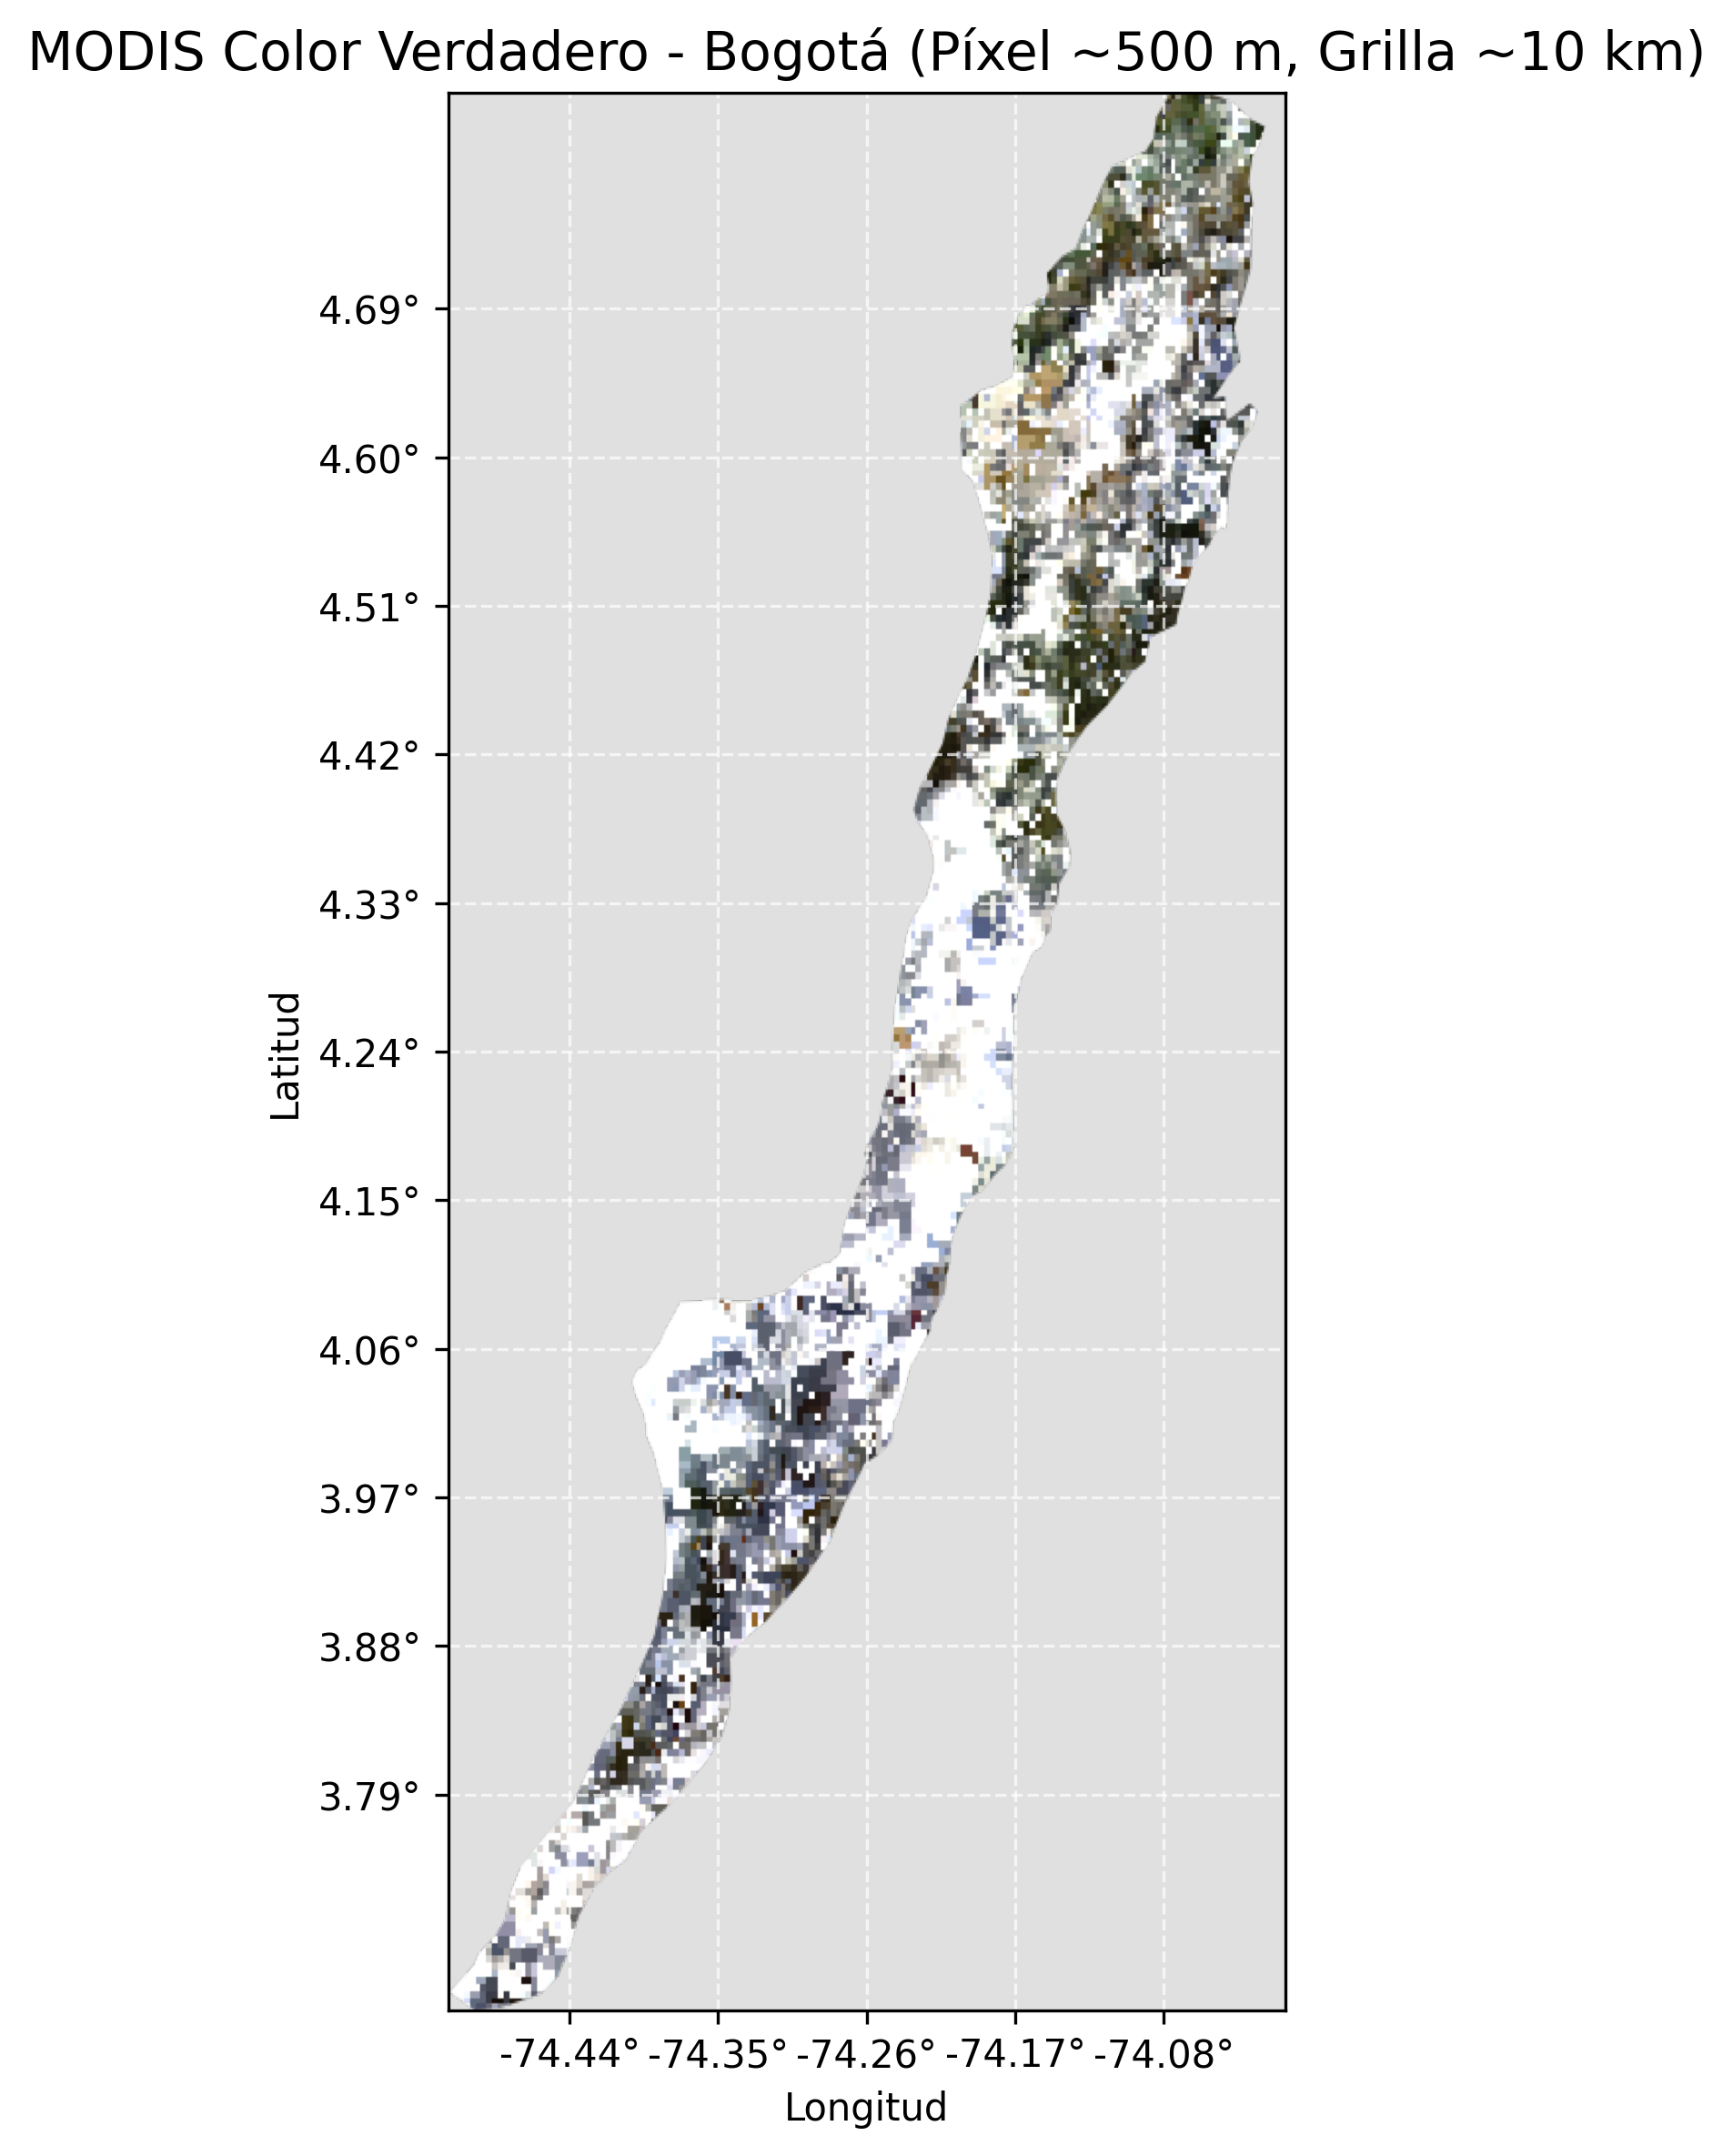
\includegraphics{45-practica_5_clase6_introduccion_sr_gee_files/figure-pdf/fig-python_modis_estatico-output-1.png}

}

\caption{\label{fig-python_modis_estatico}Imagen estática del catálogo
MODIS (Terra) en color verdadero para la ciudad de Bogotá, con grilla de
referencia.}

\end{figure}%

\subsection{Javascript}

Para ejecutar este código, debes abrir el
\textbf{\href{https://code.earthengine.google.com/}{Code Editor de
Google Earth Engine}} en tu navegador, pegar el siguiente fragmento en
la consola central y hacer clic en \textbf{``Run''}.

\phantomsection\label{js_modis}%
\begin{Shaded}
\begin{Highlighting}[]
\CommentTok{// 1. DEFINICIÓN DEL PUNTO GEOGRÁFICO}
\KeywordTok{var}\NormalTok{ punto\_unal }\OperatorTok{=}\NormalTok{ ee}\OperatorTok{.}\AttributeTok{Geometry}\OperatorTok{.}\FunctionTok{Point}\NormalTok{([}\OperatorTok{{-}}\FloatTok{74.084}\OperatorTok{,} \FloatTok{4.638}\NormalTok{])}\OperatorTok{;}

\CommentTok{// 2. CENTRAR EL VISOR}
\BuiltInTok{Map}\OperatorTok{.}\FunctionTok{centerObject}\NormalTok{(punto\_unal}\OperatorTok{,} \DecValTok{17}\NormalTok{)}\OperatorTok{;}

\CommentTok{// 3. CONSULTA Y FILTRADO DE DATOS}
\KeywordTok{var}\NormalTok{ modis }\OperatorTok{=}\NormalTok{ ee}\OperatorTok{.}\FunctionTok{ImageCollection}\NormalTok{(}\StringTok{"MODIS/061/MOD09A1"}\NormalTok{)}
  \OperatorTok{.}\FunctionTok{filterBounds}\NormalTok{(punto\_unal)}
  \OperatorTok{.}\FunctionTok{filterDate}\NormalTok{(}\StringTok{\textquotesingle{}2023{-}01{-}01\textquotesingle{}}\OperatorTok{,} \StringTok{\textquotesingle{}2023{-}12{-}31\textquotesingle{}}\NormalTok{)}
  \OperatorTok{.}\FunctionTok{first}\NormalTok{()}\OperatorTok{;}

\CommentTok{// 4. PARÁMETROS DE VISUALIZACIÓN}
\KeywordTok{var}\NormalTok{ visParams }\OperatorTok{=}\NormalTok{ \{}\DataTypeTok{bands}\OperatorTok{:}\NormalTok{ [}\StringTok{\textquotesingle{}sur\_refl\_b01\textquotesingle{}}\OperatorTok{,} \StringTok{\textquotesingle{}sur\_refl\_b04\textquotesingle{}}\OperatorTok{,} \StringTok{\textquotesingle{}sur\_refl\_b03\textquotesingle{}}\NormalTok{]}\OperatorTok{,} \DataTypeTok{min}\OperatorTok{:} \OperatorTok{{-}}\DecValTok{100}\OperatorTok{,} \DataTypeTok{max}\OperatorTok{:} \DecValTok{3000}\NormalTok{\}}\OperatorTok{;}

\CommentTok{// 5. MOSTRAR EN PANTALLA Y EN CONSOLA}
\BuiltInTok{Map}\OperatorTok{.}\FunctionTok{addLayer}\NormalTok{(modis}\OperatorTok{,}\NormalTok{ visParams}\OperatorTok{,} \StringTok{\textquotesingle{}MODIS RGB {-} UNAL Bogotá\textquotesingle{}}\NormalTok{)}\OperatorTok{;}

\FunctionTok{print}\NormalTok{(}\StringTok{\textquotesingle{}Metadatos de la imagen MODIS:\textquotesingle{}}\OperatorTok{,}\NormalTok{ modis)}\OperatorTok{;}
\FunctionTok{print}\NormalTok{(}\StringTok{\textquotesingle{}ID exacto de la imagen MODIS:\textquotesingle{}}\OperatorTok{,}\NormalTok{ modis}\OperatorTok{.}\FunctionTok{get}\NormalTok{(}\StringTok{\textquotesingle{}system:id\textquotesingle{}}\NormalTok{))}\OperatorTok{;}
\end{Highlighting}
\end{Shaded}

\begin{center}\rule{0.5\linewidth}{0.5pt}\end{center}

\phantomsection\label{js_modis_estatico}%
\begin{Shaded}
\begin{Highlighting}[]
\CommentTok{// ▷ CÓDIGO MAPA ESTÁTICO (THUMBNAIL) EN JAVASCRIPT (Independiente)}

\CommentTok{// 1. DEFINICIÓN DEL ÁREA (BOGOTÁ COMPLETA)}
\KeywordTok{var}\NormalTok{ localidades }\OperatorTok{=}\NormalTok{ ee}\OperatorTok{.}\FunctionTok{FeatureCollection}\NormalTok{(}\StringTok{"FAO/GAUL/2015/level2"}\NormalTok{)}\OperatorTok{;}
\KeywordTok{var}\NormalTok{ bogota }\OperatorTok{=}\NormalTok{ localidades}\OperatorTok{.}\FunctionTok{filter}\NormalTok{(ee}\OperatorTok{.}\AttributeTok{Filter}\OperatorTok{.}\FunctionTok{eq}\NormalTok{(}\StringTok{\textquotesingle{}ADM2\_NAME\textquotesingle{}}\OperatorTok{,} \StringTok{\textquotesingle{}Santafe De Bogota D.c.\textquotesingle{}}\NormalTok{))}\OperatorTok{;}
\KeywordTok{var}\NormalTok{ region\_interes }\OperatorTok{=}\NormalTok{ bogota}\OperatorTok{.}\FunctionTok{geometry}\NormalTok{()}\OperatorTok{.}\FunctionTok{bounds}\NormalTok{()}\OperatorTok{;}

\CommentTok{// 2. CONSULTA Y SELECCIÓN DE LA IMAGEN}
\KeywordTok{var}\NormalTok{ modis\_estatica }\OperatorTok{=}\NormalTok{ ee}\OperatorTok{.}\FunctionTok{ImageCollection}\NormalTok{(}\StringTok{"MODIS/061/MOD09A1"}\NormalTok{)}
  \OperatorTok{.}\FunctionTok{filterBounds}\NormalTok{(bogota)}
  \OperatorTok{.}\FunctionTok{filterDate}\NormalTok{(}\StringTok{\textquotesingle{}2023{-}01{-}01\textquotesingle{}}\OperatorTok{,} \StringTok{\textquotesingle{}2023{-}12{-}31\textquotesingle{}}\NormalTok{)}
  \OperatorTok{.}\FunctionTok{first}\NormalTok{()}
  \OperatorTok{.}\FunctionTok{clip}\NormalTok{(bogota)}\OperatorTok{;}

\CommentTok{// 3. PARÁMETROS DE VISUALIZACIÓN}
\KeywordTok{var}\NormalTok{ visParamsEstatica }\OperatorTok{=}\NormalTok{ \{}
  \DataTypeTok{bands}\OperatorTok{:}\NormalTok{ [}\StringTok{\textquotesingle{}sur\_refl\_b01\textquotesingle{}}\OperatorTok{,} \StringTok{\textquotesingle{}sur\_refl\_b04\textquotesingle{}}\OperatorTok{,} \StringTok{\textquotesingle{}sur\_refl\_b03\textquotesingle{}}\NormalTok{]}\OperatorTok{,}
  \DataTypeTok{min}\OperatorTok{:} \OperatorTok{{-}}\DecValTok{100}\OperatorTok{,}
  \DataTypeTok{max}\OperatorTok{:} \DecValTok{3000}\OperatorTok{,}
  \DataTypeTok{dimensions}\OperatorTok{:} \DecValTok{800}\OperatorTok{,}
  \DataTypeTok{region}\OperatorTok{:}\NormalTok{ region\_interes}
\NormalTok{\}}\OperatorTok{;}

\CommentTok{// 4. MOSTRAR EN CONSOLA LA URL Y EL THUMBNAIL}
\FunctionTok{print}\NormalTok{(}\StringTok{\textquotesingle{}URL de la imagen PNG:\textquotesingle{}}\OperatorTok{,}\NormalTok{ modis\_estatica}\OperatorTok{.}\FunctionTok{getThumbURL}\NormalTok{(visParamsEstatica))}\OperatorTok{;}

\KeywordTok{var}\NormalTok{ miniatura }\OperatorTok{=}\NormalTok{ ui}\OperatorTok{.}\FunctionTok{Thumbnail}\NormalTok{(\{}
  \DataTypeTok{image}\OperatorTok{:}\NormalTok{ modis\_estatica}\OperatorTok{,}
  \DataTypeTok{params}\OperatorTok{:}\NormalTok{ visParamsEstatica}\OperatorTok{,}
  \DataTypeTok{style}\OperatorTok{:}\NormalTok{ \{}\DataTypeTok{width}\OperatorTok{:} \StringTok{\textquotesingle{}400px\textquotesingle{}}\OperatorTok{,} \DataTypeTok{height}\OperatorTok{:} \StringTok{\textquotesingle{}400px\textquotesingle{}}\OperatorTok{,} \DataTypeTok{backgroundColor}\OperatorTok{:} \StringTok{\textquotesingle{}\#e0e0e0\textquotesingle{}}\NormalTok{\}}
\NormalTok{\})}\OperatorTok{;}
\FunctionTok{print}\NormalTok{(}\StringTok{\textquotesingle{}Vista previa estática (MODIS {-} Bogotá):\textquotesingle{}}\OperatorTok{,}\NormalTok{ miniatura)}\OperatorTok{;}
\end{Highlighting}
\end{Shaded}

\begin{center}\rule{0.5\linewidth}{0.5pt}\end{center}

\subsection{Reto: Carga de imagen en QGIS y ArcGIS
Pro}\label{reto-carga-de-imagen-en-qgis-y-arcgis-pro}

Para finalizar esta sección, replique el procedimiento de importación de
la imagen MODIS en las plataformas de escritorio.

\textbf{Instrucciones:}

\begin{enumerate}
\def\labelenumi{\arabic{enumi}.}
\tightlist
\item
  Ejecute el código de Python correspondiente a MODIS para generar el
  archivo \texttt{modis\_serializado.json} y conocer el Asset ID exacto.
\item
  En \textbf{QGIS}, emplee la pestaña \emph{Load} del plugin de GEE.
  Configure el Asset ID y defina las bandas en el orden
  \texttt{sur\_refl\_b01,sur\_refl\_b04,sur\_refl\_b03} con los valores
  mínimo y máximo establecidos en \texttt{-100} y \texttt{3000}.
\item
  En \textbf{ArcGIS Pro}, utilice la herramienta \emph{Add Image to Map
  by Serialized Object} o, alternativamente, \emph{Add Image to Map by
  Asset ID}.
\item
  \textbf{Reporte:} Tome las respectivas capturas de pantalla de la
  configuración de la herramienta antes de su ejecución e insértelas
  reemplazando las rutas indicadas a continuación.
\end{enumerate}

\begin{quote}
\textbf{Reporte visual de MODIS}

\emph{Captura de QGIS (Pestaña Load):}
\texttt{!{[}Parámetros\ de\ MODIS\ en\ QGIS{]}(ruta/a/tu/captura\_qgis\_modis.png)\{fig-align="center"\ width="80\%"\}}

\emph{Captura de ArcGIS Pro (Herramienta utilizada):}
\texttt{!{[}Parámetros\ de\ MODIS\ en\ ArcGIS\ Pro{]}(ruta/a/tu/captura\_arcgis\_modis.png)\{fig-align="center"\ width="80\%"\}}
\end{quote}

\section{Catálogo de datos: SRTM (modelo digital de
elevación)}\label{catuxe1logo-de-datos-srtm-modelo-digital-de-elevaciuxf3n}

Datos de topografía global. La misión Shuttle Radar Topography Mission
(SRTM) provee un modelo de elevación a nivel casi global. En este
ejercicio, además de acceder al dato base de altitud, aplicaremos una
función de servidor para calcular un mapa de sombras (\emph{hillshade}),
lo cual facilita la interpretación visual del relieve terrestre.

\begin{longtable}[]{@{}lll@{}}
\toprule\noalign{}
Banda & Resolución & Descripción \\
\midrule\noalign{}
\endhead
\bottomrule\noalign{}
\endlastfoot
elevation & 30m & Elevación en metros sobre el nivel medio del mar \\
\end{longtable}

\subsection{Python}

\begin{Shaded}
\begin{Highlighting}[]
\CommentTok{\# \#| eval: false}

\CommentTok{\# Código usando Folium!}

\ImportTok{import}\NormalTok{ ee}
\ImportTok{import}\NormalTok{ folium}
\ImportTok{import}\NormalTok{ json}

\CommentTok{\# 1. DEFINICIÓN DEL PUNTO GEOGRÁFICO}
\NormalTok{unal\_punto }\OperatorTok{=}\NormalTok{ ee.Geometry.Point([}\OperatorTok{{-}}\FloatTok{74.084}\NormalTok{, }\FloatTok{4.638}\NormalTok{])}

\CommentTok{\# 2. CARGA DE DATOS Y PROCESAMIENTO}
\NormalTok{srtm }\OperatorTok{=}\NormalTok{ ee.Image(}\StringTok{"USGS/SRTMGL1\_003"}\NormalTok{)}
\NormalTok{hillshade }\OperatorTok{=}\NormalTok{ ee.Terrain.hillshade(srtm)}

\CommentTok{\# 3. EXPORTAR LOS ARCHIVOS JSON (METADATOS Y SERIALIZADO)}
\NormalTok{id\_exacto }\OperatorTok{=}\NormalTok{ srtm.get(}\StringTok{\textquotesingle{}system:id\textquotesingle{}}\NormalTok{).getInfo()}
\BuiltInTok{print}\NormalTok{(}\SpecialStringTok{f"}\CharTok{\textbackslash{}n}\SpecialStringTok{ID de la imagen SRTM seleccionada: }\SpecialCharTok{\{}\NormalTok{id\_exacto}\SpecialCharTok{\}}\SpecialStringTok{"}\NormalTok{)}

\NormalTok{metadatos\_json }\OperatorTok{=}\NormalTok{ srtm.getInfo()}
\ControlFlowTok{with} \BuiltInTok{open}\NormalTok{(}\StringTok{\textquotesingle{}metadatos\_srtm.json\textquotesingle{}}\NormalTok{, }\StringTok{\textquotesingle{}w\textquotesingle{}}\NormalTok{) }\ImportTok{as}\NormalTok{ archivo:}
\NormalTok{    json.dump(metadatos\_json, archivo, indent}\OperatorTok{=}\DecValTok{4}\NormalTok{)}

\NormalTok{srtm\_limpia }\OperatorTok{=}\NormalTok{ ee.Image(id\_exacto)}
\NormalTok{texto\_json\_serializado }\OperatorTok{=}\NormalTok{ srtm\_limpia.serialize()}
\ControlFlowTok{with} \BuiltInTok{open}\NormalTok{(}\StringTok{\textquotesingle{}srtm\_serializado.json\textquotesingle{}}\NormalTok{, }\StringTok{\textquotesingle{}w\textquotesingle{}}\NormalTok{) }\ImportTok{as}\NormalTok{ archivo:}
\NormalTok{    json.dump(texto\_json\_serializado, archivo)}

\CommentTok{\# 4. PARÁMETROS DE VISUALIZACIÓN}
\NormalTok{vis\_params }\OperatorTok{=}\NormalTok{ \{}\StringTok{\textquotesingle{}min\textquotesingle{}}\NormalTok{: }\DecValTok{0}\NormalTok{, }\StringTok{\textquotesingle{}max\textquotesingle{}}\NormalTok{: }\DecValTok{255}\NormalTok{\}}
\NormalTok{map\_id\_dict }\OperatorTok{=}\NormalTok{ ee.Image(hillshade).getMapId(vis\_params)}

\CommentTok{\# 5. MENSAJE FINAL}
\BuiltInTok{print}\NormalTok{(}\StringTok{"}\CharTok{\textbackslash{}n}\StringTok{✅ MAPA GENERADO CON ÉXITO"}\NormalTok{)}
\BuiltInTok{print}\NormalTok{(}\StringTok{"Capa desplegada : Relieve SRTM"}\NormalTok{)}
\BuiltInTok{print}\NormalTok{(}\StringTok{"{-}{-}{-}{-}{-}{-}{-}{-}{-}{-}{-}{-}{-}{-}{-}{-}{-}{-}{-}{-}{-}{-}{-}{-}{-}{-}{-}{-}{-}{-}{-}{-}{-}{-}{-}{-}{-}{-}{-}{-}{-}{-}{-}{-}{-}{-}{-}{-}{-}{-}{-}{-}{-}{-}{-}{-}{-}{-}{-}{-}{-}{-}{-}{-}"}\NormalTok{)}

\CommentTok{\# 6. CONFIGURACIÓN DEL MAPA BASE (Folium)}
\NormalTok{Map\_srtm }\OperatorTok{=}\NormalTok{ folium.Map(location}\OperatorTok{=}\NormalTok{[}\FloatTok{4.638}\NormalTok{, }\OperatorTok{{-}}\FloatTok{74.084}\NormalTok{], zoom\_start}\OperatorTok{=}\DecValTok{17}\NormalTok{)}

\CommentTok{\# 7. AGREGAR LA IMAGEN AL VISOR}
\NormalTok{folium.TileLayer(}
\NormalTok{    tiles}\OperatorTok{=}\NormalTok{map\_id\_dict[}\StringTok{\textquotesingle{}tile\_fetcher\textquotesingle{}}\NormalTok{].url\_format,}
\NormalTok{    attr}\OperatorTok{=}\StringTok{\textquotesingle{}Google Earth Engine\textquotesingle{}}\NormalTok{,}
\NormalTok{    overlay}\OperatorTok{=}\VariableTok{True}\NormalTok{,}
\NormalTok{    name}\OperatorTok{=}\StringTok{\textquotesingle{}Relieve SRTM\textquotesingle{}}
\NormalTok{).add\_to(Map\_srtm)}

\NormalTok{folium.LayerControl().add\_to(Map\_srtm)}

\CommentTok{\# 8. VISUALIZACIÓN DEL RESULTADO}
\CommentTok{\# Map\_srtm}
\CommentTok{\# from IPython.display import display, HTML}
\CommentTok{\# display(HTML(Map\_srtm.\_repr\_html\_()))}

\ImportTok{from}\NormalTok{ IPython.display }\ImportTok{import}\NormalTok{ IFrame}

\CommentTok{\# Guardamos el mapa aislado en tu carpeta de trabajo}
\NormalTok{Map\_srtm.save(}\StringTok{"mapas/map\_srtm.html"}\NormalTok{)}

\CommentTok{\# Lo incrustamos en el documento Quarto como una página web independiente}
\NormalTok{display(IFrame(src}\OperatorTok{=}\StringTok{"mapas/map\_srtm.html"}\NormalTok{, width}\OperatorTok{=}\StringTok{"100\%"}\NormalTok{, height}\OperatorTok{=}\StringTok{"500px"}\NormalTok{))}
\end{Highlighting}
\end{Shaded}

\begin{verbatim}

ID de la imagen SRTM seleccionada: USGS/SRTMGL1_003

✅ MAPA GENERADO CON ÉXITO
Capa desplegada : Relieve SRTM
----------------------------------------------------------------
\end{verbatim}

\phantomsection\label{python_srtm}
\begin{verbatim}
<IPython.lib.display.IFrame at 0x7ac2a2f8a570>
\end{verbatim}

\begin{center}\rule{0.5\linewidth}{0.5pt}\end{center}

\begin{Shaded}
\begin{Highlighting}[]
\CommentTok{\# \#| eval: false}

\CommentTok{\# ▷ CÓDIGO MAPA ESTÁTICO (PNG) PARA FOLIUM/GENERAL (Independiente)}
\ImportTok{import}\NormalTok{ ee}
\ImportTok{import}\NormalTok{ requests}
\ImportTok{import}\NormalTok{ matplotlib.pyplot }\ImportTok{as}\NormalTok{ plt}
\ImportTok{from}\NormalTok{ PIL }\ImportTok{import}\NormalTok{ Image}
\ImportTok{from}\NormalTok{ io }\ImportTok{import}\NormalTok{ BytesIO}

\CommentTok{\# 1. DEFINICIÓN DEL PUNTO GEOGRÁFICO Y REGIÓN DE INTERÉS}
\NormalTok{lon\_centro, lat\_centro }\OperatorTok{=} \OperatorTok{{-}}\FloatTok{74.084}\NormalTok{, }\FloatTok{4.638}
\NormalTok{unal\_punto }\OperatorTok{=}\NormalTok{ ee.Geometry.Point([lon\_centro, lat\_centro])}
\NormalTok{region\_interes }\OperatorTok{=}\NormalTok{ unal\_punto.}\BuiltInTok{buffer}\NormalTok{(}\DecValTok{3000}\NormalTok{)}

\CommentTok{\# 2. CONSULTA Y PROCESAMIENTO DE LA IMAGEN}
\NormalTok{srtm\_estatica }\OperatorTok{=}\NormalTok{ ee.Image(}\StringTok{"USGS/SRTMGL1\_003"}\NormalTok{)}
\NormalTok{hillshade\_estatica }\OperatorTok{=}\NormalTok{ ee.Terrain.hillshade(srtm\_estatica)}

\CommentTok{\# 3. OBTENER LA URL DEL THUMBNAIL (PNG) DESDE GOOGLE EARTH ENGINE}
\NormalTok{url\_img }\OperatorTok{=}\NormalTok{ hillshade\_estatica.getThumbURL(\{}
    \StringTok{\textquotesingle{}min\textquotesingle{}}\NormalTok{: }\DecValTok{0}\NormalTok{,}
    \StringTok{\textquotesingle{}max\textquotesingle{}}\NormalTok{: }\DecValTok{255}\NormalTok{,}
    \StringTok{\textquotesingle{}dimensions\textquotesingle{}}\NormalTok{: }\DecValTok{800}\NormalTok{,}
    \StringTok{\textquotesingle{}region\textquotesingle{}}\NormalTok{: region\_interes}
\NormalTok{\})}

\CommentTok{\# 4. DESCARGAR Y DIBUJAR LA IMAGEN CON MATPLOTLIB}
\NormalTok{respuesta }\OperatorTok{=}\NormalTok{ requests.get(url\_img)}
\NormalTok{imagen\_png }\OperatorTok{=}\NormalTok{ Image.}\BuiltInTok{open}\NormalTok{(BytesIO(respuesta.content))}

\CommentTok{\# Obtenemos las coordenadas límite para georreferenciar la imagen PNG}
\NormalTok{coords }\OperatorTok{=}\NormalTok{ region\_interes.bounds().coordinates().get(}\DecValTok{0}\NormalTok{).getInfo()}
\NormalTok{xmin, ymin }\OperatorTok{=}\NormalTok{ coords[}\DecValTok{0}\NormalTok{][}\DecValTok{0}\NormalTok{], coords[}\DecValTok{0}\NormalTok{][}\DecValTok{1}\NormalTok{]}
\NormalTok{xmax, ymax }\OperatorTok{=}\NormalTok{ coords[}\DecValTok{2}\NormalTok{][}\DecValTok{0}\NormalTok{], coords[}\DecValTok{2}\NormalTok{][}\DecValTok{1}\NormalTok{]}

\NormalTok{fig, ax }\OperatorTok{=}\NormalTok{ plt.subplots(figsize}\OperatorTok{=}\NormalTok{(}\DecValTok{8}\NormalTok{, }\DecValTok{8}\NormalTok{))}

\CommentTok{\# Mapeamos los píxeles a grados}
\NormalTok{ax.imshow(imagen\_png, cmap}\OperatorTok{=}\StringTok{\textquotesingle{}gray\textquotesingle{}}\NormalTok{, extent}\OperatorTok{=}\NormalTok{[xmin, xmax, ymin, ymax])}

\CommentTok{\# Grilla de 1 km. (1 grado ≈ 111 km {-}\textgreater{} 1 km ≈ 0.009 grados)}
\NormalTok{paso\_1km }\OperatorTok{=} \FloatTok{0.009} 

\NormalTok{x\_ticks }\OperatorTok{=}\NormalTok{ [lon\_centro }\OperatorTok{+}\NormalTok{ (i }\OperatorTok{*}\NormalTok{ paso\_1km) }\ControlFlowTok{for}\NormalTok{ i }\KeywordTok{in} \BuiltInTok{range}\NormalTok{(}\OperatorTok{{-}}\DecValTok{4}\NormalTok{, }\DecValTok{5}\NormalTok{)]}
\NormalTok{y\_ticks }\OperatorTok{=}\NormalTok{ [lat\_centro }\OperatorTok{+}\NormalTok{ (i }\OperatorTok{*}\NormalTok{ paso\_1km) }\ControlFlowTok{for}\NormalTok{ i }\KeywordTok{in} \BuiltInTok{range}\NormalTok{(}\OperatorTok{{-}}\DecValTok{4}\NormalTok{, }\DecValTok{5}\NormalTok{)]}

\NormalTok{x\_ticks }\OperatorTok{=}\NormalTok{ [x }\ControlFlowTok{for}\NormalTok{ x }\KeywordTok{in}\NormalTok{ x\_ticks }\ControlFlowTok{if}\NormalTok{ xmin }\OperatorTok{\textless{}=}\NormalTok{ x }\OperatorTok{\textless{}=}\NormalTok{ xmax]}
\NormalTok{y\_ticks }\OperatorTok{=}\NormalTok{ [y }\ControlFlowTok{for}\NormalTok{ y }\KeywordTok{in}\NormalTok{ y\_ticks }\ControlFlowTok{if}\NormalTok{ ymin }\OperatorTok{\textless{}=}\NormalTok{ y }\OperatorTok{\textless{}=}\NormalTok{ ymax]}

\NormalTok{ax.set\_xticks(x\_ticks)}
\NormalTok{ax.set\_yticks(y\_ticks)}
\NormalTok{ax.set\_xticklabels([}\SpecialStringTok{f"}\SpecialCharTok{\{}\NormalTok{x}\SpecialCharTok{:.3f\}}\SpecialStringTok{°"} \ControlFlowTok{for}\NormalTok{ x }\KeywordTok{in}\NormalTok{ x\_ticks])}
\NormalTok{ax.set\_yticklabels([}\SpecialStringTok{f"}\SpecialCharTok{\{}\NormalTok{y}\SpecialCharTok{:.3f\}}\SpecialStringTok{°"} \ControlFlowTok{for}\NormalTok{ y }\KeywordTok{in}\NormalTok{ y\_ticks])}

\NormalTok{ax.grid(color}\OperatorTok{=}\StringTok{\textquotesingle{}white\textquotesingle{}}\NormalTok{, linestyle}\OperatorTok{=}\StringTok{\textquotesingle{}{-}{-}\textquotesingle{}}\NormalTok{, linewidth}\OperatorTok{=}\FloatTok{0.8}\NormalTok{, alpha}\OperatorTok{=}\FloatTok{0.5}\NormalTok{)}
\NormalTok{ax.set\_title(}\StringTok{\textquotesingle{}Relieve SRTM (Píxel \textasciitilde{}30 m, Grilla \textasciitilde{}1 km)\textquotesingle{}}\NormalTok{, fontsize}\OperatorTok{=}\DecValTok{14}\NormalTok{)}
\NormalTok{ax.set\_xlabel(}\StringTok{\textquotesingle{}Longitud\textquotesingle{}}\NormalTok{)}
\NormalTok{ax.set\_ylabel(}\StringTok{\textquotesingle{}Latitud\textquotesingle{}}\NormalTok{)}

\NormalTok{plt.tight\_layout()}
\NormalTok{plt.show()}
\end{Highlighting}
\end{Shaded}

\begin{figure}[H]

\centering{

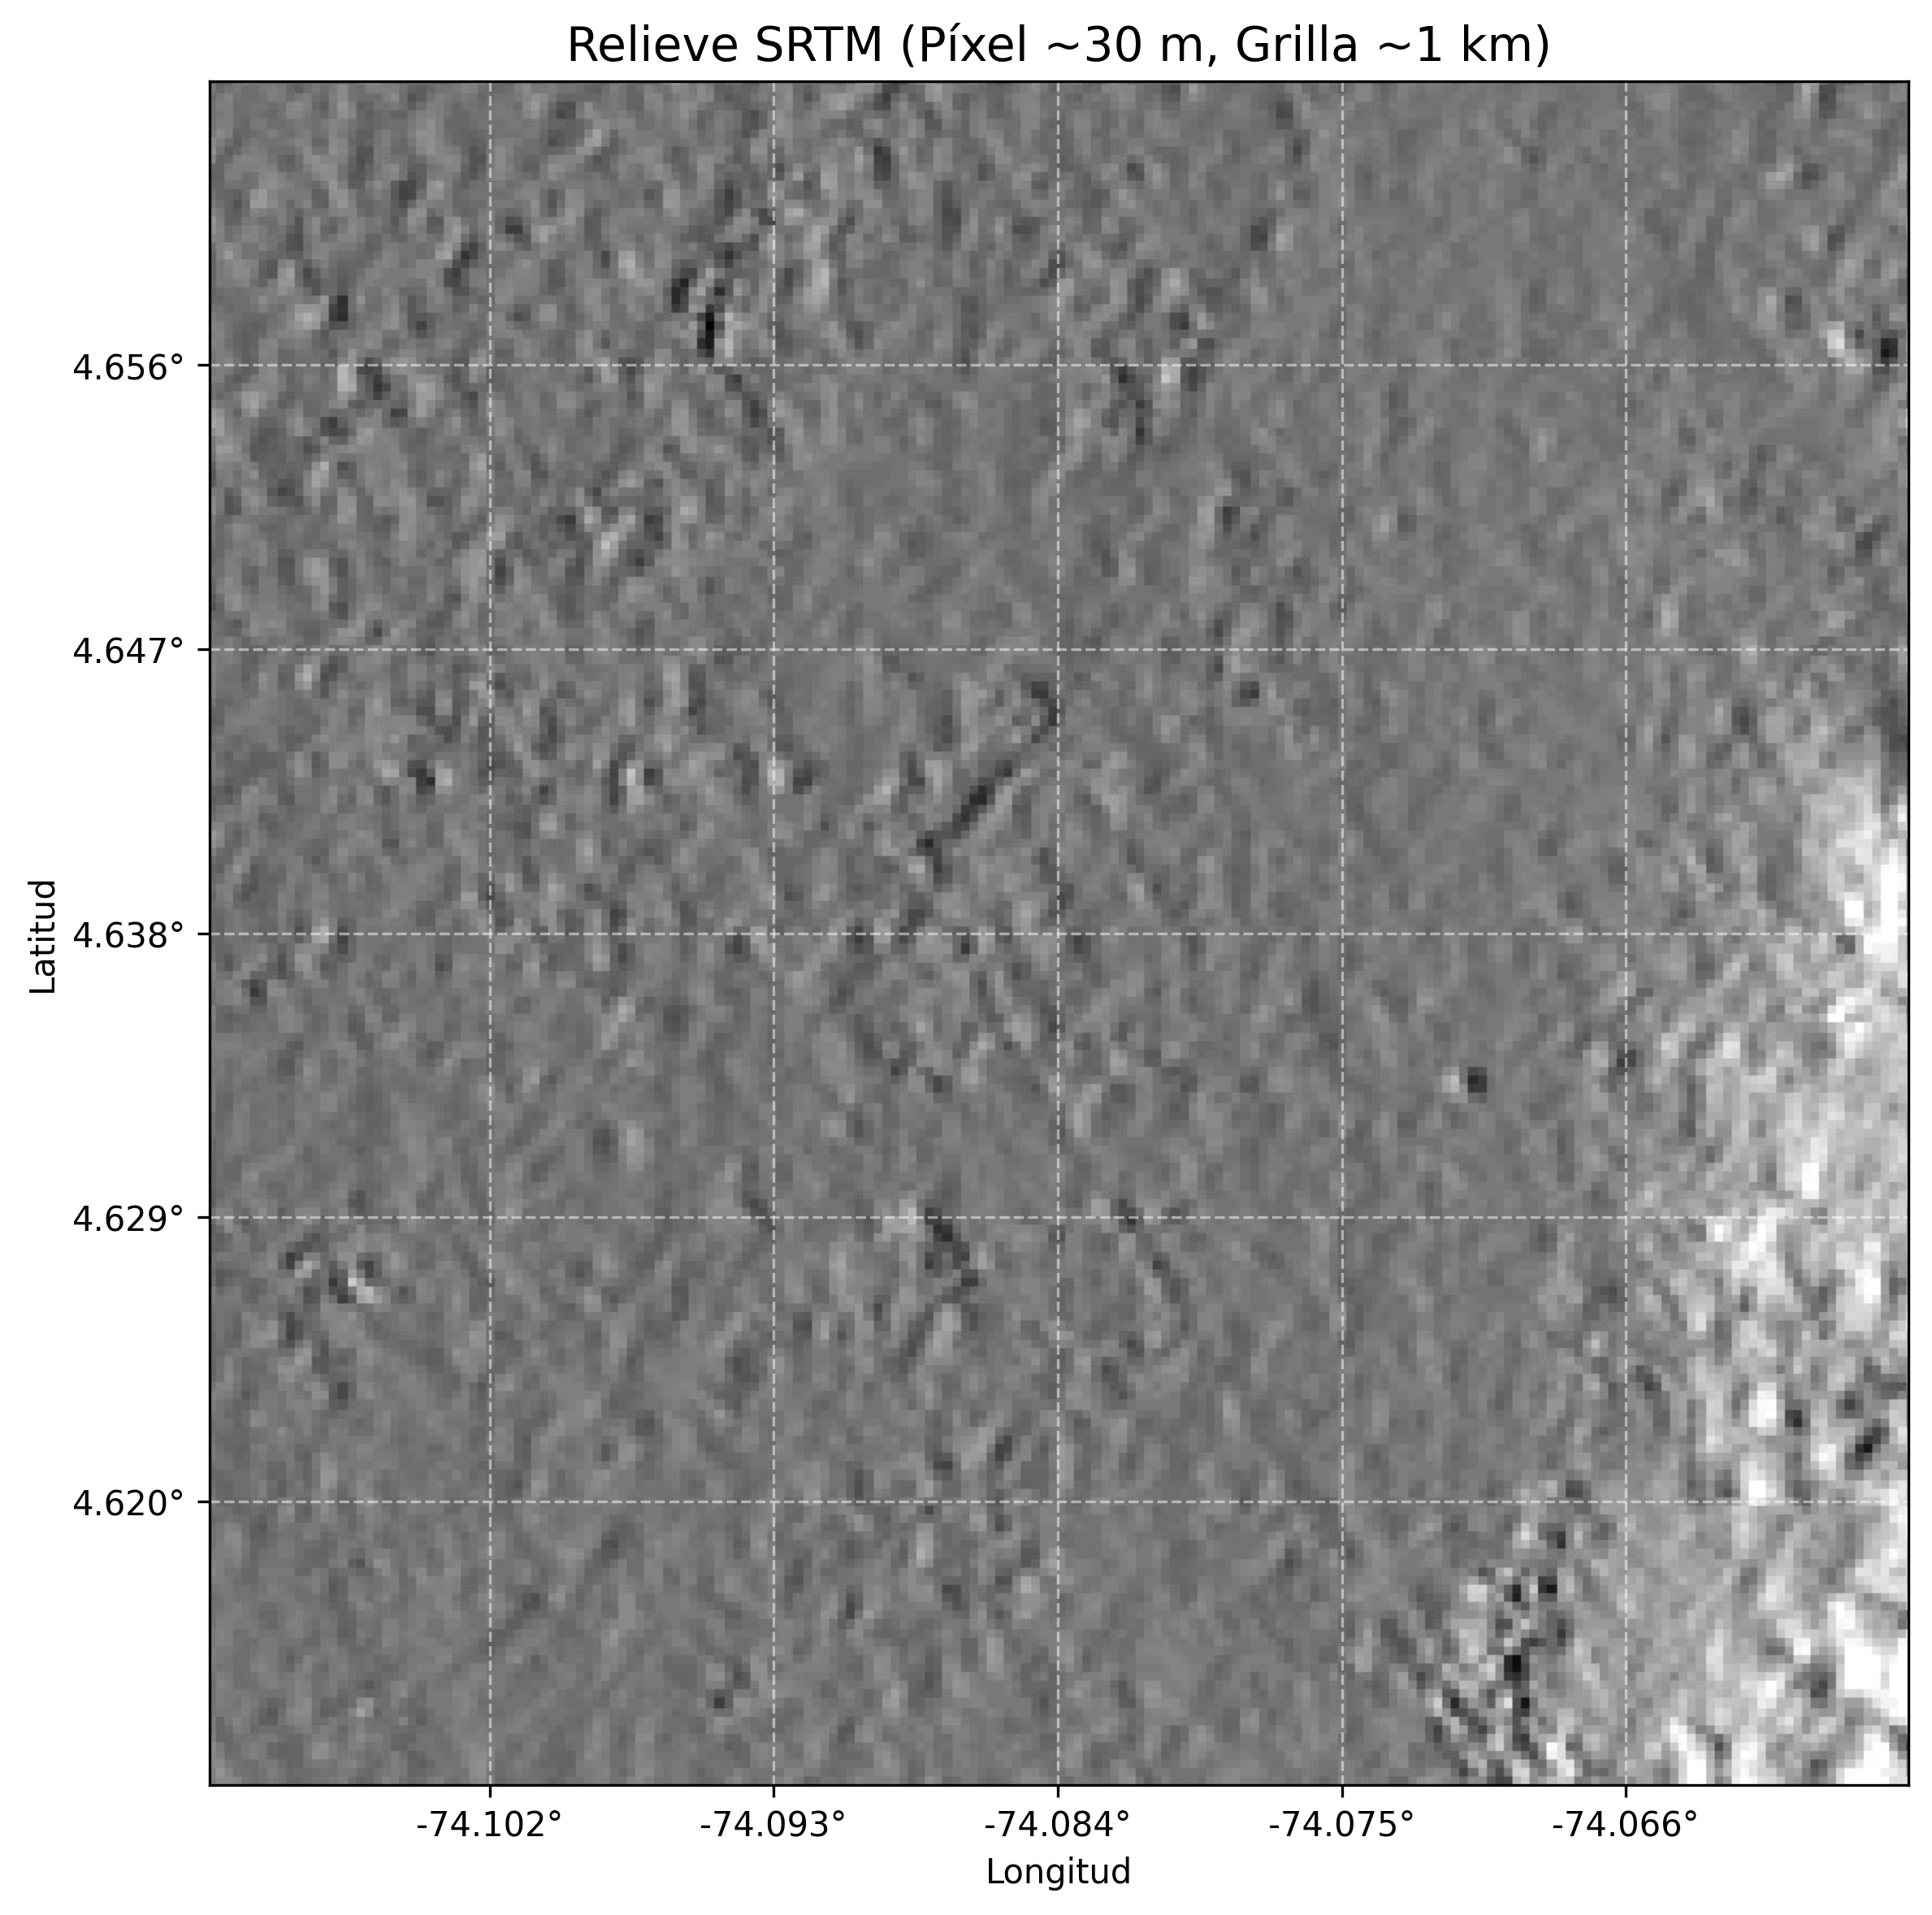
\includegraphics{45-practica_5_clase6_introduccion_sr_gee_files/figure-pdf/fig-python_srtm_estatico-output-1.png}

}

\caption{\label{fig-python_srtm_estatico}Mapa estático de relieve
sombreado (Hillshade) derivado del Modelo Digital de Elevación SRTM con
grilla de referencia.}

\end{figure}%

\subsection{Javascript}

Para ejecutar este código, debes abrir el
\textbf{\href{https://code.earthengine.google.com/}{Code Editor de
Google Earth Engine}} en tu navegador, pegar el siguiente fragmento en
la consola central y hacer clic en \textbf{``Run''}.

\phantomsection\label{js_srtm}%
\begin{Shaded}
\begin{Highlighting}[]
\CommentTok{// 1. DEFINICIÓN DEL PUNTO GEOGRÁFICO}
\KeywordTok{var}\NormalTok{ punto\_unal }\OperatorTok{=}\NormalTok{ ee}\OperatorTok{.}\AttributeTok{Geometry}\OperatorTok{.}\FunctionTok{Point}\NormalTok{([}\OperatorTok{{-}}\FloatTok{74.084}\OperatorTok{,} \FloatTok{4.638}\NormalTok{])}\OperatorTok{;}

\CommentTok{// 2. CENTRAR EL VISOR}
\BuiltInTok{Map}\OperatorTok{.}\FunctionTok{centerObject}\NormalTok{(punto\_unal}\OperatorTok{,} \DecValTok{17}\NormalTok{)}\OperatorTok{;}

\CommentTok{// 3. CONSULTA Y FILTRADO DE DATOS}
\KeywordTok{var}\NormalTok{ srtm }\OperatorTok{=}\NormalTok{ ee}\OperatorTok{.}\FunctionTok{Image}\NormalTok{(}\StringTok{"USGS/SRTMGL1\_003"}\NormalTok{)}\OperatorTok{;}
\KeywordTok{var}\NormalTok{ hillshade }\OperatorTok{=}\NormalTok{ ee}\OperatorTok{.}\AttributeTok{Terrain}\OperatorTok{.}\FunctionTok{hillshade}\NormalTok{(srtm)}\OperatorTok{;}

\CommentTok{// 4. PARÁMETROS DE VISUALIZACIÓN}
\KeywordTok{var}\NormalTok{ visParams }\OperatorTok{=}\NormalTok{ \{}\DataTypeTok{min}\OperatorTok{:} \DecValTok{0}\OperatorTok{,} \DataTypeTok{max}\OperatorTok{:} \DecValTok{255}\NormalTok{\}}\OperatorTok{;}

\CommentTok{// 5. MOSTRAR EN PANTALLA Y EN CONSOLA}
\BuiltInTok{Map}\OperatorTok{.}\FunctionTok{addLayer}\NormalTok{(hillshade}\OperatorTok{,}\NormalTok{ visParams}\OperatorTok{,} \StringTok{\textquotesingle{}Relieve SRTM {-} UNAL Bogotá\textquotesingle{}}\NormalTok{)}\OperatorTok{;}

\FunctionTok{print}\NormalTok{(}\StringTok{\textquotesingle{}Metadatos de la imagen SRTM:\textquotesingle{}}\OperatorTok{,}\NormalTok{ srtm)}\OperatorTok{;}
\FunctionTok{print}\NormalTok{(}\StringTok{\textquotesingle{}ID exacto de la imagen SRTM:\textquotesingle{}}\OperatorTok{,}\NormalTok{ srtm}\OperatorTok{.}\FunctionTok{get}\NormalTok{(}\StringTok{\textquotesingle{}system:id\textquotesingle{}}\NormalTok{))}\OperatorTok{;}
\end{Highlighting}
\end{Shaded}

\begin{center}\rule{0.5\linewidth}{0.5pt}\end{center}

\phantomsection\label{js_srtm_estatico}%
\begin{Shaded}
\begin{Highlighting}[]
\CommentTok{// ▷ CÓDIGO MAPA ESTÁTICO (THUMBNAIL) EN JAVASCRIPT (Independiente)}

\CommentTok{// 1. DEFINICIÓN DEL PUNTO Y REGIÓN DE INTERÉS}
\KeywordTok{var}\NormalTok{ punto\_unal }\OperatorTok{=}\NormalTok{ ee}\OperatorTok{.}\AttributeTok{Geometry}\OperatorTok{.}\FunctionTok{Point}\NormalTok{([}\OperatorTok{{-}}\FloatTok{74.084}\OperatorTok{,} \FloatTok{4.638}\NormalTok{])}\OperatorTok{;}
\KeywordTok{var}\NormalTok{ region\_interes }\OperatorTok{=}\NormalTok{ punto\_unal}\OperatorTok{.}\FunctionTok{buffer}\NormalTok{(}\DecValTok{3000}\NormalTok{)}\OperatorTok{;} 

\CommentTok{// 2. CONSULTA Y PROCESAMIENTO DE LA IMAGEN}
\KeywordTok{var}\NormalTok{ srtm\_estatica }\OperatorTok{=}\NormalTok{ ee}\OperatorTok{.}\FunctionTok{Image}\NormalTok{(}\StringTok{"USGS/SRTMGL1\_003"}\NormalTok{)}\OperatorTok{;}
\KeywordTok{var}\NormalTok{ hillshade\_estatica }\OperatorTok{=}\NormalTok{ ee}\OperatorTok{.}\AttributeTok{Terrain}\OperatorTok{.}\FunctionTok{hillshade}\NormalTok{(srtm\_estatica)}\OperatorTok{;}

\CommentTok{// 3. PARÁMETROS DE VISUALIZACIÓN}
\KeywordTok{var}\NormalTok{ visParamsEstatica }\OperatorTok{=}\NormalTok{ \{}
  \DataTypeTok{min}\OperatorTok{:} \DecValTok{0}\OperatorTok{,}
  \DataTypeTok{max}\OperatorTok{:} \DecValTok{255}\OperatorTok{,}
  \DataTypeTok{dimensions}\OperatorTok{:} \DecValTok{800}\OperatorTok{,}
  \DataTypeTok{region}\OperatorTok{:}\NormalTok{ region\_interes}
\NormalTok{\}}\OperatorTok{;}

\CommentTok{// 4. MOSTRAR EN CONSOLA LA URL Y EL THUMBNAIL}
\FunctionTok{print}\NormalTok{(}\StringTok{\textquotesingle{}URL de la imagen PNG:\textquotesingle{}}\OperatorTok{,}\NormalTok{ hillshade\_estatica}\OperatorTok{.}\FunctionTok{getThumbURL}\NormalTok{(visParamsEstatica))}\OperatorTok{;}

\KeywordTok{var}\NormalTok{ miniatura }\OperatorTok{=}\NormalTok{ ui}\OperatorTok{.}\FunctionTok{Thumbnail}\NormalTok{(\{}
  \DataTypeTok{image}\OperatorTok{:}\NormalTok{ hillshade\_estatica}\OperatorTok{,}
  \DataTypeTok{params}\OperatorTok{:}\NormalTok{ visParamsEstatica}\OperatorTok{,}
  \DataTypeTok{style}\OperatorTok{:}\NormalTok{ \{}\DataTypeTok{width}\OperatorTok{:} \StringTok{\textquotesingle{}400px\textquotesingle{}}\OperatorTok{,} \DataTypeTok{height}\OperatorTok{:} \StringTok{\textquotesingle{}400px\textquotesingle{}}\NormalTok{\}}
\NormalTok{\})}\OperatorTok{;}
\FunctionTok{print}\NormalTok{(}\StringTok{\textquotesingle{}Vista previa estática (Relieve SRTM):\textquotesingle{}}\OperatorTok{,}\NormalTok{ miniatura)}\OperatorTok{;}
\end{Highlighting}
\end{Shaded}

\begin{center}\rule{0.5\linewidth}{0.5pt}\end{center}

\subsection{Reto: Carga de imagen en QGIS y ArcGIS
Pro}\label{reto-carga-de-imagen-en-qgis-y-arcgis-pro-1}

Replique el procedimiento de importación del Modelo Digital de Elevación
en las plataformas de escritorio utilizando el Asset ID.

\textbf{Instrucciones:}

\begin{enumerate}
\def\labelenumi{\arabic{enumi}.}
\tightlist
\item
  Ejecute el código de Python correspondiente a SRTM para generar el
  archivo \texttt{srtm\_serializado.json} y confirmar el Asset ID
  exacto.
\item
  En \textbf{QGIS}, emplee la pestaña \emph{Load} del plugin de GEE.
  Configure el Asset ID \texttt{USGS/SRTMGL1\_003} y defina el rango de
  visualización adecuado.
\item
  En \textbf{ArcGIS Pro}, utilice la herramienta \emph{Add Image to Map
  by Serialized Object} o la herramienta \emph{Add Image to Map by Asset
  ID}.
\item
  \textbf{Reporte:} Tome las respectivas capturas de pantalla de la
  configuración de la herramienta antes de su ejecución e insértelas
  reemplazando las rutas indicadas a continuación.
\end{enumerate}

\begin{quote}
\textbf{Reporte visual de SRTM}

\emph{Captura de QGIS (Pestaña Load):}
\texttt{!{[}Parámetros\ de\ SRTM\ en\ QGIS{]}(ruta/a/tu/captura\_qgis\_srtm.png)\{fig-align="center"\ width="80\%"\}}

\emph{Captura de ArcGIS Pro (Herramienta utilizada):}
\texttt{!{[}Parámetros\ de\ SRTM\ en\ ArcGIS\ Pro{]}(ruta/a/tu/captura\_arcgis\_srtm.png)\{fig-align="center"\ width="80\%"\}}
\end{quote}

\section{Catálogo de datos: CHIRPS (datos de clima /
precipitación)}\label{catuxe1logo-de-datos-chirps-datos-de-clima-precipitaciuxf3n}

Datos climáticos de alta resolución temporal. El conjunto de datos
CHIRPS (\emph{Climate Hazards Group InfraRed Precipitation with Station
data}) combina observaciones satelitales infrarrojas con datos de
estaciones terrestres para estimar la cantidad de lluvia diaria.

\begin{longtable}[]{@{}lll@{}}
\toprule\noalign{}
Banda & Resolución & Descripción \\
\midrule\noalign{}
\endhead
\bottomrule\noalign{}
\endlastfoot
precipitation & 5.5km & Precipitación diaria (mm) \\
\end{longtable}

\subsection{Python}

\begin{Shaded}
\begin{Highlighting}[]
\CommentTok{\# \#| eval: false}

\CommentTok{\# Código usando Folium!}

\ImportTok{import}\NormalTok{ ee}
\ImportTok{import}\NormalTok{ folium}
\ImportTok{import}\NormalTok{ datetime}
\ImportTok{import}\NormalTok{ json}

\CommentTok{\# 1. DEFINICIÓN DEL PUNTO GEOGRÁFICO}
\NormalTok{unal\_punto }\OperatorTok{=}\NormalTok{ ee.Geometry.Point([}\OperatorTok{{-}}\FloatTok{74.084}\NormalTok{, }\FloatTok{4.638}\NormalTok{])}

\CommentTok{\# 2. EXPLORAR TODAS LAS OPCIONES Y FILTRAR}
\NormalTok{coleccion\_clima }\OperatorTok{=}\NormalTok{ (ee.ImageCollection(}\StringTok{"UCSB{-}CHG/CHIRPS/DAILY"}\NormalTok{)}
\NormalTok{    .filterBounds(unal\_punto)}
\NormalTok{    .filterDate(}\StringTok{\textquotesingle{}2023{-}05{-}01\textquotesingle{}}\NormalTok{, }\StringTok{\textquotesingle{}2023{-}05{-}31\textquotesingle{}}\NormalTok{))}

\CommentTok{\# 3. DIAGNÓSTICO: EXTRAER EL TOP 3 DE IMÁGENES}
\NormalTok{ids }\OperatorTok{=}\NormalTok{ coleccion\_clima.aggregate\_array(}\StringTok{\textquotesingle{}system:id\textquotesingle{}}\NormalTok{).getInfo()}
\NormalTok{fechas }\OperatorTok{=}\NormalTok{ coleccion\_clima.aggregate\_array(}\StringTok{\textquotesingle{}system:time\_start\textquotesingle{}}\NormalTok{).getInfo()}

\BuiltInTok{print}\NormalTok{(}\StringTok{"{-}{-}{-} TOP 3 IMÁGENES CHIRPS (MAYO 2023) {-}{-}{-}"}\NormalTok{)}
\ControlFlowTok{for}\NormalTok{ i }\KeywordTok{in} \BuiltInTok{range}\NormalTok{(}\BuiltInTok{min}\NormalTok{(}\DecValTok{3}\NormalTok{, }\BuiltInTok{len}\NormalTok{(ids))):}
\NormalTok{    fecha\_legible }\OperatorTok{=}\NormalTok{ datetime.datetime.fromtimestamp(fechas[i] }\OperatorTok{/} \FloatTok{1000.0}\NormalTok{, datetime.UTC).strftime(}\StringTok{\textquotesingle{}\%Y{-}\%m{-}}\SpecialCharTok{\%d}\StringTok{\textquotesingle{}}\NormalTok{)}
    \BuiltInTok{print}\NormalTok{(}\SpecialStringTok{f"Opción }\SpecialCharTok{\{}\NormalTok{i}\OperatorTok{+}\DecValTok{1}\SpecialCharTok{\}}\SpecialStringTok{ | Fecha: }\SpecialCharTok{\{}\NormalTok{fecha\_legible}\SpecialCharTok{\}}\SpecialStringTok{"}\NormalTok{)}
    \BuiltInTok{print}\NormalTok{(}\SpecialStringTok{f"ID: }\SpecialCharTok{\{}\NormalTok{ids[i]}\SpecialCharTok{\}}\CharTok{\textbackslash{}n}\SpecialStringTok{"}\NormalTok{)}
\BuiltInTok{print}\NormalTok{(}\StringTok{"{-}{-}{-}{-}{-}{-}{-}{-}{-}{-}{-}{-}{-}{-}{-}{-}{-}{-}{-}{-}{-}{-}{-}{-}{-}{-}{-}{-}{-}{-}{-}{-}{-}{-}{-}{-}{-}{-}{-}{-}{-}{-}{-}{-}{-}{-}{-}{-}{-}{-}{-}{-}{-}{-}{-}{-}{-}{-}{-}{-}{-}{-}{-}{-}"}\NormalTok{)}

\CommentTok{\# 4. SELECCIÓN DEFINITIVA DE LA IMAGEN}
\NormalTok{chirps }\OperatorTok{=}\NormalTok{ ee.Image(coleccion\_clima.first())}

\CommentTok{\# 5. EXPORTAR LOS ARCHIVOS JSON (METADATOS Y SERIALIZADO)}
\NormalTok{id\_exacto }\OperatorTok{=}\NormalTok{ chirps.get(}\StringTok{\textquotesingle{}system:id\textquotesingle{}}\NormalTok{).getInfo()}
\BuiltInTok{print}\NormalTok{(}\SpecialStringTok{f"}\CharTok{\textbackslash{}n}\SpecialStringTok{ID de la imagen CHIRPS seleccionada: }\SpecialCharTok{\{}\NormalTok{id\_exacto}\SpecialCharTok{\}}\SpecialStringTok{"}\NormalTok{)}

\NormalTok{metadatos\_json }\OperatorTok{=}\NormalTok{ chirps.getInfo()}
\ControlFlowTok{with} \BuiltInTok{open}\NormalTok{(}\StringTok{\textquotesingle{}metadatos\_chirps.json\textquotesingle{}}\NormalTok{, }\StringTok{\textquotesingle{}w\textquotesingle{}}\NormalTok{) }\ImportTok{as}\NormalTok{ archivo:}
\NormalTok{    json.dump(metadatos\_json, archivo, indent}\OperatorTok{=}\DecValTok{4}\NormalTok{)}

\NormalTok{chirps\_limpia }\OperatorTok{=}\NormalTok{ ee.Image(id\_exacto)}
\NormalTok{texto\_json\_serializado }\OperatorTok{=}\NormalTok{ chirps\_limpia.serialize()}
\ControlFlowTok{with} \BuiltInTok{open}\NormalTok{(}\StringTok{\textquotesingle{}chirps\_serializado.json\textquotesingle{}}\NormalTok{, }\StringTok{\textquotesingle{}w\textquotesingle{}}\NormalTok{) }\ImportTok{as}\NormalTok{ archivo:}
\NormalTok{    json.dump(texto\_json\_serializado, archivo)}

\CommentTok{\# 6. PARÁMETROS DE VISUALIZACIÓN}
\NormalTok{vis\_params }\OperatorTok{=}\NormalTok{ \{}\StringTok{\textquotesingle{}bands\textquotesingle{}}\NormalTok{: [}\StringTok{\textquotesingle{}precipitation\textquotesingle{}}\NormalTok{], }\StringTok{\textquotesingle{}min\textquotesingle{}}\NormalTok{: }\DecValTok{0}\NormalTok{, }\StringTok{\textquotesingle{}max\textquotesingle{}}\NormalTok{: }\DecValTok{50}\NormalTok{, }\StringTok{\textquotesingle{}palette\textquotesingle{}}\NormalTok{: [}\StringTok{\textquotesingle{}white\textquotesingle{}}\NormalTok{, }\StringTok{\textquotesingle{}blue\textquotesingle{}}\NormalTok{]\}}
\NormalTok{map\_id\_dict }\OperatorTok{=}\NormalTok{ ee.Image(chirps).getMapId(vis\_params)}

\CommentTok{\# 7. MENSAJE FINAL}
\NormalTok{fecha\_capa\_ms }\OperatorTok{=}\NormalTok{ chirps.get(}\StringTok{\textquotesingle{}system:time\_start\textquotesingle{}}\NormalTok{).getInfo()}
\NormalTok{fecha\_capa }\OperatorTok{=}\NormalTok{ datetime.datetime.fromtimestamp(fecha\_capa\_ms }\OperatorTok{/} \FloatTok{1000.0}\NormalTok{, datetime.UTC).strftime(}\StringTok{\textquotesingle{}\%Y{-}\%m{-}}\SpecialCharTok{\%d}\StringTok{\textquotesingle{}}\NormalTok{)}

\BuiltInTok{print}\NormalTok{(}\StringTok{"}\CharTok{\textbackslash{}n}\StringTok{✅ MAPA GENERADO CON ÉXITO"}\NormalTok{)}
\BuiltInTok{print}\NormalTok{(}\SpecialStringTok{f"Capa desplegada : Precipitación {-} }\SpecialCharTok{\{}\NormalTok{fecha\_capa}\SpecialCharTok{\}}\SpecialStringTok{"}\NormalTok{)}
\BuiltInTok{print}\NormalTok{(}\StringTok{"{-}{-}{-}{-}{-}{-}{-}{-}{-}{-}{-}{-}{-}{-}{-}{-}{-}{-}{-}{-}{-}{-}{-}{-}{-}{-}{-}{-}{-}{-}{-}{-}{-}{-}{-}{-}{-}{-}{-}{-}{-}{-}{-}{-}{-}{-}{-}{-}{-}{-}{-}{-}{-}{-}{-}{-}{-}{-}{-}{-}{-}{-}{-}{-}"}\NormalTok{)}

\CommentTok{\# 8. CONFIGURACIÓN DEL MAPA BASE (Folium)}
\NormalTok{Map\_clima }\OperatorTok{=}\NormalTok{ folium.Map(location}\OperatorTok{=}\NormalTok{[}\FloatTok{4.638}\NormalTok{, }\OperatorTok{{-}}\FloatTok{74.084}\NormalTok{], zoom\_start}\OperatorTok{=}\DecValTok{17}\NormalTok{)}

\CommentTok{\# 9. AGREGAR LA IMAGEN AL VISOR}
\NormalTok{folium.TileLayer(}
\NormalTok{    tiles}\OperatorTok{=}\NormalTok{map\_id\_dict[}\StringTok{\textquotesingle{}tile\_fetcher\textquotesingle{}}\NormalTok{].url\_format,}
\NormalTok{    attr}\OperatorTok{=}\StringTok{\textquotesingle{}Google Earth Engine\textquotesingle{}}\NormalTok{,}
\NormalTok{    overlay}\OperatorTok{=}\VariableTok{True}\NormalTok{,}
\NormalTok{    name}\OperatorTok{=}\SpecialStringTok{f\textquotesingle{}Precipitación {-} }\SpecialCharTok{\{}\NormalTok{fecha\_capa}\SpecialCharTok{\}}\SpecialStringTok{\textquotesingle{}}
\NormalTok{).add\_to(Map\_clima)}

\NormalTok{folium.LayerControl().add\_to(Map\_clima)}

\CommentTok{\# 10. VISUALIZACIÓN DEL RESULTADO}
\CommentTok{\# Map\_clima}
\CommentTok{\# from IPython.display import display, HTML}
\CommentTok{\# display(HTML(Map\_clima.\_repr\_html\_()))}

\ImportTok{from}\NormalTok{ IPython.display }\ImportTok{import}\NormalTok{ IFrame}

\CommentTok{\# Guardamos el mapa aislado en tu carpeta de trabajo}
\NormalTok{Map\_clima.save(}\StringTok{"mapas/map\_clima.html"}\NormalTok{)}

\CommentTok{\# Lo incrustamos en el documento Quarto como una página web independiente}
\NormalTok{display(IFrame(src}\OperatorTok{=}\StringTok{"mapas/map\_clima.html"}\NormalTok{, width}\OperatorTok{=}\StringTok{"100\%"}\NormalTok{, height}\OperatorTok{=}\StringTok{"500px"}\NormalTok{))}
\end{Highlighting}
\end{Shaded}

\begin{verbatim}
--- TOP 3 IMÁGENES CHIRPS (MAYO 2023) ---
Opción 1 | Fecha: 2023-05-01
ID: UCSB-CHG/CHIRPS/DAILY/20230501

Opción 2 | Fecha: 2023-05-02
ID: UCSB-CHG/CHIRPS/DAILY/20230502

Opción 3 | Fecha: 2023-05-03
ID: UCSB-CHG/CHIRPS/DAILY/20230503

----------------------------------------------------------------

ID de la imagen CHIRPS seleccionada: UCSB-CHG/CHIRPS/DAILY/20230501

✅ MAPA GENERADO CON ÉXITO
Capa desplegada : Precipitación - 2023-05-01
----------------------------------------------------------------
\end{verbatim}

\phantomsection\label{python_clima}
\begin{verbatim}
<IPython.lib.display.IFrame at 0x7ac2a2ebcec0>
\end{verbatim}

\begin{center}\rule{0.5\linewidth}{0.5pt}\end{center}

\begin{Shaded}
\begin{Highlighting}[]
\CommentTok{\# \#| eval: false}

\CommentTok{\# ▷ CÓDIGO MAPA ESTÁTICO (PNG) PARA FOLIUM/GENERAL (Independiente)}
\ImportTok{import}\NormalTok{ ee}
\ImportTok{import}\NormalTok{ requests}
\ImportTok{import}\NormalTok{ matplotlib.pyplot }\ImportTok{as}\NormalTok{ plt}
\ImportTok{from}\NormalTok{ matplotlib.colors }\ImportTok{import}\NormalTok{ Normalize, LinearSegmentedColormap}
\ImportTok{from}\NormalTok{ matplotlib.cm }\ImportTok{import}\NormalTok{ ScalarMappable}
\ImportTok{from}\NormalTok{ PIL }\ImportTok{import}\NormalTok{ Image}
\ImportTok{from}\NormalTok{ io }\ImportTok{import}\NormalTok{ BytesIO}

\CommentTok{\# 1. DEFINICIÓN DEL ÁREA (CUNDINAMARCA COMPLETA)}
\NormalTok{departamentos }\OperatorTok{=}\NormalTok{ ee.FeatureCollection(}\StringTok{"FAO/GAUL/2015/level1"}\NormalTok{)}
\NormalTok{cundinamarca }\OperatorTok{=}\NormalTok{ departamentos.}\BuiltInTok{filter}\NormalTok{(ee.Filter.eq(}\StringTok{\textquotesingle{}ADM1\_NAME\textquotesingle{}}\NormalTok{, }\StringTok{\textquotesingle{}Cundinamarca\textquotesingle{}}\NormalTok{))}
\NormalTok{region\_interes }\OperatorTok{=}\NormalTok{ cundinamarca.geometry().bounds()}

\CommentTok{\# 2. CONSULTA Y PROCESAMIENTO DE LA IMAGEN}
\NormalTok{chirps\_estatica }\OperatorTok{=}\NormalTok{ ee.ImageCollection(}\StringTok{"UCSB{-}CHG/CHIRPS/DAILY"}\NormalTok{)}\OperatorTok{\textbackslash{}}
\NormalTok{    .filterBounds(cundinamarca)}\OperatorTok{\textbackslash{}}
\NormalTok{    .filterDate(}\StringTok{\textquotesingle{}2023{-}05{-}01\textquotesingle{}}\NormalTok{, }\StringTok{\textquotesingle{}2023{-}05{-}31\textquotesingle{}}\NormalTok{)}\OperatorTok{\textbackslash{}}
\NormalTok{    .first()}\OperatorTok{\textbackslash{}}
\NormalTok{    .clip(cundinamarca)}

\CommentTok{\# 3. EXTRAER VALORES MÍNIMO Y MÁXIMO REALES DE LA IMAGEN}
\NormalTok{stats }\OperatorTok{=}\NormalTok{ chirps\_estatica.reduceRegion(}
\NormalTok{    reducer}\OperatorTok{=}\NormalTok{ee.Reducer.minMax(),}
\NormalTok{    geometry}\OperatorTok{=}\NormalTok{cundinamarca.geometry(),}
\NormalTok{    scale}\OperatorTok{=}\DecValTok{5566}\NormalTok{,}
\NormalTok{    maxPixels}\OperatorTok{=}\FloatTok{1e9}
\NormalTok{).getInfo()}

\NormalTok{val\_min }\OperatorTok{=}\NormalTok{ stats.get(}\StringTok{\textquotesingle{}precipitation\_min\textquotesingle{}}\NormalTok{, }\DecValTok{0}\NormalTok{)}
\NormalTok{val\_max }\OperatorTok{=}\NormalTok{ stats.get(}\StringTok{\textquotesingle{}precipitation\_max\textquotesingle{}}\NormalTok{, }\DecValTok{50}\NormalTok{)}

\ControlFlowTok{if}\NormalTok{ val\_min }\OperatorTok{==}\NormalTok{ val\_max:}
\NormalTok{    val\_max }\OperatorTok{=}\NormalTok{ val\_min }\OperatorTok{+} \FloatTok{1.0}

\CommentTok{\# 4. OBTENER LA URL DEL THUMBNAIL (PNG) DESDE GOOGLE EARTH ENGINE}
\NormalTok{url\_img }\OperatorTok{=}\NormalTok{ chirps\_estatica.getThumbURL(\{}
    \StringTok{\textquotesingle{}bands\textquotesingle{}}\NormalTok{: [}\StringTok{\textquotesingle{}precipitation\textquotesingle{}}\NormalTok{],}
    \StringTok{\textquotesingle{}min\textquotesingle{}}\NormalTok{: val\_min,}
    \StringTok{\textquotesingle{}max\textquotesingle{}}\NormalTok{: val\_max,}
    \StringTok{\textquotesingle{}palette\textquotesingle{}}\NormalTok{: [}\StringTok{\textquotesingle{}white\textquotesingle{}}\NormalTok{, }\StringTok{\textquotesingle{}blue\textquotesingle{}}\NormalTok{],}
    \StringTok{\textquotesingle{}dimensions\textquotesingle{}}\NormalTok{: }\DecValTok{800}\NormalTok{,}
    \StringTok{\textquotesingle{}region\textquotesingle{}}\NormalTok{: region\_interes}
\NormalTok{\})}

\CommentTok{\# 5. DESCARGAR Y DIBUJAR LA IMAGEN CON MATPLOTLIB (Con Grilla)}
\NormalTok{respuesta }\OperatorTok{=}\NormalTok{ requests.get(url\_img)}
\NormalTok{imagen\_png }\OperatorTok{=}\NormalTok{ Image.}\BuiltInTok{open}\NormalTok{(BytesIO(respuesta.content))}

\CommentTok{\# Obtenemos las coordenadas límite para georreferenciar la imagen PNG}
\NormalTok{coords }\OperatorTok{=}\NormalTok{ region\_interes.coordinates().get(}\DecValTok{0}\NormalTok{).getInfo()}
\NormalTok{xmin }\OperatorTok{=} \BuiltInTok{min}\NormalTok{([c[}\DecValTok{0}\NormalTok{] }\ControlFlowTok{for}\NormalTok{ c }\KeywordTok{in}\NormalTok{ coords])}
\NormalTok{xmax }\OperatorTok{=} \BuiltInTok{max}\NormalTok{([c[}\DecValTok{0}\NormalTok{] }\ControlFlowTok{for}\NormalTok{ c }\KeywordTok{in}\NormalTok{ coords])}
\NormalTok{ymin }\OperatorTok{=} \BuiltInTok{min}\NormalTok{([c[}\DecValTok{1}\NormalTok{] }\ControlFlowTok{for}\NormalTok{ c }\KeywordTok{in}\NormalTok{ coords])}
\NormalTok{ymax }\OperatorTok{=} \BuiltInTok{max}\NormalTok{([c[}\DecValTok{1}\NormalTok{] }\ControlFlowTok{for}\NormalTok{ c }\KeywordTok{in}\NormalTok{ coords])}

\NormalTok{fig, ax }\OperatorTok{=}\NormalTok{ plt.subplots(figsize}\OperatorTok{=}\NormalTok{(}\DecValTok{8}\NormalTok{, }\DecValTok{8}\NormalTok{))}
\NormalTok{ax.imshow(imagen\_png, extent}\OperatorTok{=}\NormalTok{[xmin, xmax, ymin, ymax])}

\CommentTok{\# Grilla de 25 km. (1 grado ≈ 111 km {-}\textgreater{} 25 km ≈ 0.25 grados)}
\NormalTok{paso\_25km }\OperatorTok{=} \FloatTok{0.25} 
\NormalTok{lon\_centro, lat\_centro }\OperatorTok{=}\NormalTok{ (xmin }\OperatorTok{+}\NormalTok{ xmax) }\OperatorTok{/} \DecValTok{2}\NormalTok{, (ymin }\OperatorTok{+}\NormalTok{ ymax) }\OperatorTok{/} \DecValTok{2}

\NormalTok{x\_ticks }\OperatorTok{=}\NormalTok{ [lon\_centro }\OperatorTok{+}\NormalTok{ (i }\OperatorTok{*}\NormalTok{ paso\_25km) }\ControlFlowTok{for}\NormalTok{ i }\KeywordTok{in} \BuiltInTok{range}\NormalTok{(}\OperatorTok{{-}}\DecValTok{5}\NormalTok{, }\DecValTok{6}\NormalTok{) }\ControlFlowTok{if}\NormalTok{ xmin }\OperatorTok{\textless{}=}\NormalTok{ lon\_centro }\OperatorTok{+}\NormalTok{ (i }\OperatorTok{*}\NormalTok{ paso\_25km) }\OperatorTok{\textless{}=}\NormalTok{ xmax]}
\NormalTok{y\_ticks }\OperatorTok{=}\NormalTok{ [lat\_centro }\OperatorTok{+}\NormalTok{ (i }\OperatorTok{*}\NormalTok{ paso\_25km) }\ControlFlowTok{for}\NormalTok{ i }\KeywordTok{in} \BuiltInTok{range}\NormalTok{(}\OperatorTok{{-}}\DecValTok{5}\NormalTok{, }\DecValTok{6}\NormalTok{) }\ControlFlowTok{if}\NormalTok{ ymin }\OperatorTok{\textless{}=}\NormalTok{ lat\_centro }\OperatorTok{+}\NormalTok{ (i }\OperatorTok{*}\NormalTok{ paso\_25km) }\OperatorTok{\textless{}=}\NormalTok{ ymax]}

\NormalTok{ax.set\_xticks(x\_ticks)}
\NormalTok{ax.set\_yticks(y\_ticks)}
\NormalTok{ax.set\_xticklabels([}\SpecialStringTok{f"}\SpecialCharTok{\{}\NormalTok{x}\SpecialCharTok{:.2f\}}\SpecialStringTok{°"} \ControlFlowTok{for}\NormalTok{ x }\KeywordTok{in}\NormalTok{ x\_ticks])}
\NormalTok{ax.set\_yticklabels([}\SpecialStringTok{f"}\SpecialCharTok{\{}\NormalTok{y}\SpecialCharTok{:.2f\}}\SpecialStringTok{°"} \ControlFlowTok{for}\NormalTok{ y }\KeywordTok{in}\NormalTok{ y\_ticks])}

\NormalTok{ax.grid(color}\OperatorTok{=}\StringTok{\textquotesingle{}gray\textquotesingle{}}\NormalTok{, linestyle}\OperatorTok{=}\StringTok{\textquotesingle{}{-}{-}\textquotesingle{}}\NormalTok{, linewidth}\OperatorTok{=}\FloatTok{0.8}\NormalTok{, alpha}\OperatorTok{=}\FloatTok{0.5}\NormalTok{)}
\NormalTok{ax.set\_title(}\StringTok{\textquotesingle{}Precipitación CHIRPS {-} Cundinamarca (Píxel \textasciitilde{}5.5 km, Grilla \textasciitilde{}25 km)\textquotesingle{}}\NormalTok{, fontsize}\OperatorTok{=}\DecValTok{14}\NormalTok{)}
\NormalTok{ax.set\_xlabel(}\StringTok{\textquotesingle{}Longitud\textquotesingle{}}\NormalTok{)}
\NormalTok{ax.set\_ylabel(}\StringTok{\textquotesingle{}Latitud\textquotesingle{}}\NormalTok{)}
\NormalTok{ax.set\_facecolor(}\StringTok{\textquotesingle{}\#e0e0e0\textquotesingle{}}\NormalTok{)}

\CommentTok{\# 6. AGREGAR LEYENDA (COLORBAR) DINÁMICA}
\NormalTok{cmap\_custom }\OperatorTok{=}\NormalTok{ LinearSegmentedColormap.from\_list(}\StringTok{"chirps\_cmap"}\NormalTok{, [}\StringTok{\textquotesingle{}white\textquotesingle{}}\NormalTok{, }\StringTok{\textquotesingle{}blue\textquotesingle{}}\NormalTok{])}
\NormalTok{norm }\OperatorTok{=}\NormalTok{ Normalize(vmin}\OperatorTok{=}\NormalTok{val\_min, vmax}\OperatorTok{=}\NormalTok{val\_max)}
\NormalTok{cbar }\OperatorTok{=}\NormalTok{ fig.colorbar(ScalarMappable(norm}\OperatorTok{=}\NormalTok{norm, cmap}\OperatorTok{=}\NormalTok{cmap\_custom), ax}\OperatorTok{=}\NormalTok{ax, shrink}\OperatorTok{=}\FloatTok{0.75}\NormalTok{, pad}\OperatorTok{=}\FloatTok{0.04}\NormalTok{)}
\NormalTok{cbar.set\_label(}\StringTok{\textquotesingle{}Precipitación (mm/día)\textquotesingle{}}\NormalTok{, rotation}\OperatorTok{=}\DecValTok{270}\NormalTok{, labelpad}\OperatorTok{=}\DecValTok{15}\NormalTok{)}

\NormalTok{plt.tight\_layout()}
\NormalTok{plt.show()}
\end{Highlighting}
\end{Shaded}

\begin{figure}[H]

\centering{

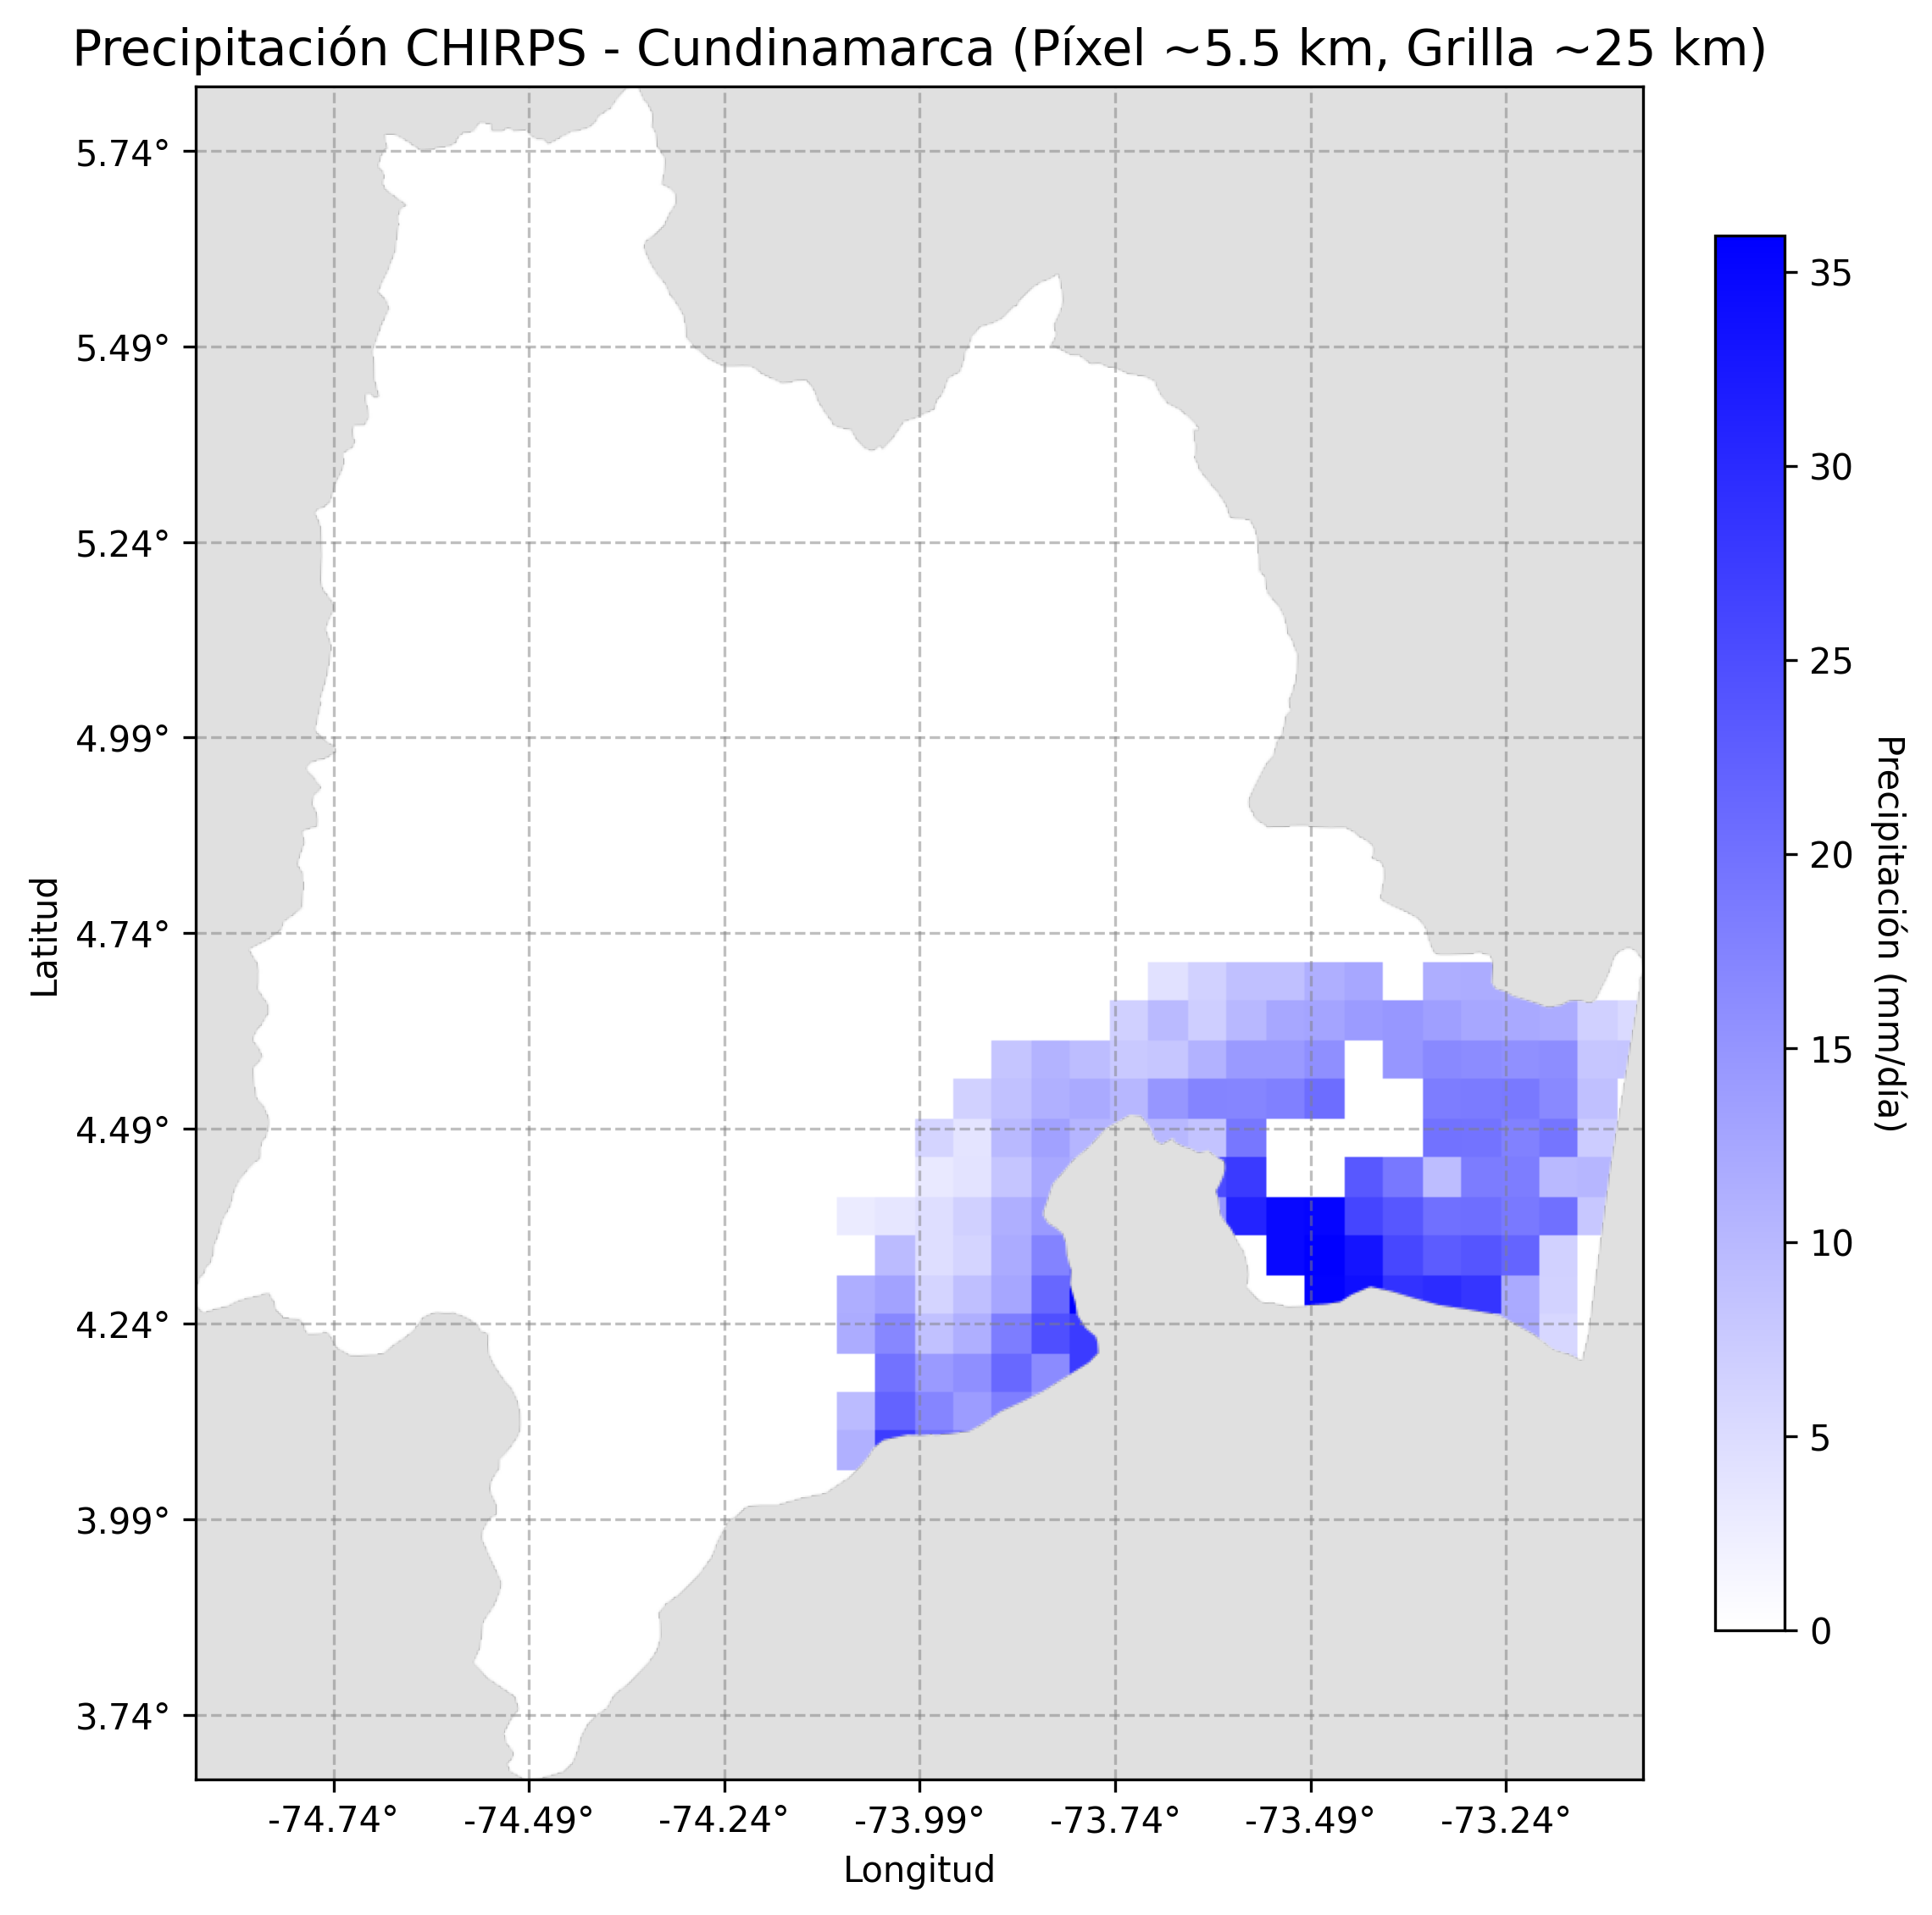
\includegraphics{45-practica_5_clase6_introduccion_sr_gee_files/figure-pdf/fig-python_clima_estatico-output-1.png}

}

\caption{\label{fig-python_clima_estatico}Mapa estático de precipitación
diaria (CHIRPS) para el departamento de Cundinamarca, con leyenda de
valores dinámicos y grilla espacial de \textasciitilde25 km.}

\end{figure}%

\subsection{Javascript}

Para ejecutar este código, debes abrir el
\textbf{\href{https://code.earthengine.google.com/}{Code Editor de
Google Earth Engine}} en tu navegador, pegar el siguiente fragmento en
la consola central y hacer clic en \textbf{``Run''}.

\phantomsection\label{js_clima}%
\begin{Shaded}
\begin{Highlighting}[]
\CommentTok{// 1. DEFINICIÓN DEL PUNTO GEOGRÁFICO}
\KeywordTok{var}\NormalTok{ punto\_unal }\OperatorTok{=}\NormalTok{ ee}\OperatorTok{.}\AttributeTok{Geometry}\OperatorTok{.}\FunctionTok{Point}\NormalTok{([}\OperatorTok{{-}}\FloatTok{74.084}\OperatorTok{,} \FloatTok{4.638}\NormalTok{])}\OperatorTok{;}

\CommentTok{// 2. CENTRAR EL VISOR}
\BuiltInTok{Map}\OperatorTok{.}\FunctionTok{centerObject}\NormalTok{(punto\_unal}\OperatorTok{,} \DecValTok{17}\NormalTok{)}\OperatorTok{;}

\CommentTok{// 3. CONSULTA Y FILTRADO DE DATOS}
\KeywordTok{var}\NormalTok{ chirps }\OperatorTok{=}\NormalTok{ ee}\OperatorTok{.}\FunctionTok{ImageCollection}\NormalTok{(}\StringTok{"UCSB{-}CHG/CHIRPS/DAILY"}\NormalTok{)}
  \OperatorTok{.}\FunctionTok{filterBounds}\NormalTok{(punto\_unal)}
  \OperatorTok{.}\FunctionTok{filterDate}\NormalTok{(}\StringTok{\textquotesingle{}2023{-}05{-}01\textquotesingle{}}\OperatorTok{,} \StringTok{\textquotesingle{}2023{-}05{-}31\textquotesingle{}}\NormalTok{)}
  \OperatorTok{.}\FunctionTok{first}\NormalTok{()}\OperatorTok{;}

\CommentTok{// 4. PARÁMETROS DE VISUALIZACIÓN}
\KeywordTok{var}\NormalTok{ visParams }\OperatorTok{=}\NormalTok{ \{}\DataTypeTok{bands}\OperatorTok{:}\NormalTok{ [}\StringTok{\textquotesingle{}precipitation\textquotesingle{}}\NormalTok{]}\OperatorTok{,} \DataTypeTok{min}\OperatorTok{:} \DecValTok{0}\OperatorTok{,} \DataTypeTok{max}\OperatorTok{:} \DecValTok{50}\OperatorTok{,} \DataTypeTok{palette}\OperatorTok{:}\NormalTok{ [}\StringTok{\textquotesingle{}white\textquotesingle{}}\OperatorTok{,} \StringTok{\textquotesingle{}blue\textquotesingle{}}\NormalTok{]\}}\OperatorTok{;}

\CommentTok{// 5. MOSTRAR EN PANTALLA Y EN CONSOLA}
\BuiltInTok{Map}\OperatorTok{.}\FunctionTok{addLayer}\NormalTok{(chirps}\OperatorTok{,}\NormalTok{ visParams}\OperatorTok{,} \StringTok{\textquotesingle{}Precipitación CHIRPS {-} UNAL Bogotá\textquotesingle{}}\NormalTok{)}\OperatorTok{;}

\FunctionTok{print}\NormalTok{(}\StringTok{\textquotesingle{}Metadatos de la imagen CHIRPS:\textquotesingle{}}\OperatorTok{,}\NormalTok{ chirps)}\OperatorTok{;}
\FunctionTok{print}\NormalTok{(}\StringTok{\textquotesingle{}ID exacto de la imagen CHIRPS:\textquotesingle{}}\OperatorTok{,}\NormalTok{ chirps}\OperatorTok{.}\FunctionTok{get}\NormalTok{(}\StringTok{\textquotesingle{}system:id\textquotesingle{}}\NormalTok{))}\OperatorTok{;}
\end{Highlighting}
\end{Shaded}

\begin{center}\rule{0.5\linewidth}{0.5pt}\end{center}

\phantomsection\label{js_clima_estatico}%
\begin{Shaded}
\begin{Highlighting}[]
\CommentTok{// ▷ CÓDIGO MAPA ESTÁTICO (THUMBNAIL) EN JAVASCRIPT (Independiente)}

\CommentTok{// 1. DEFINICIÓN DEL ÁREA (CUNDINAMARCA COMPLETA)}
\KeywordTok{var}\NormalTok{ departamentos }\OperatorTok{=}\NormalTok{ ee}\OperatorTok{.}\FunctionTok{FeatureCollection}\NormalTok{(}\StringTok{"FAO/GAUL/2015/level1"}\NormalTok{)}\OperatorTok{;}
\KeywordTok{var}\NormalTok{ cundinamarca }\OperatorTok{=}\NormalTok{ departamentos}\OperatorTok{.}\FunctionTok{filter}\NormalTok{(ee}\OperatorTok{.}\AttributeTok{Filter}\OperatorTok{.}\FunctionTok{eq}\NormalTok{(}\StringTok{\textquotesingle{}ADM1\_NAME\textquotesingle{}}\OperatorTok{,} \StringTok{\textquotesingle{}Cundinamarca\textquotesingle{}}\NormalTok{))}\OperatorTok{;}
\KeywordTok{var}\NormalTok{ region\_interes }\OperatorTok{=}\NormalTok{ cundinamarca}\OperatorTok{.}\FunctionTok{geometry}\NormalTok{()}\OperatorTok{.}\FunctionTok{bounds}\NormalTok{()}\OperatorTok{;}

\CommentTok{// 2. CONSULTA Y PROCESAMIENTO DE LA IMAGEN}
\KeywordTok{var}\NormalTok{ chirps\_estatica }\OperatorTok{=}\NormalTok{ ee}\OperatorTok{.}\FunctionTok{ImageCollection}\NormalTok{(}\StringTok{"UCSB{-}CHG/CHIRPS/DAILY"}\NormalTok{)}
  \OperatorTok{.}\FunctionTok{filterBounds}\NormalTok{(cundinamarca)}
  \OperatorTok{.}\FunctionTok{filterDate}\NormalTok{(}\StringTok{\textquotesingle{}2023{-}05{-}01\textquotesingle{}}\OperatorTok{,} \StringTok{\textquotesingle{}2023{-}05{-}31\textquotesingle{}}\NormalTok{)}
  \OperatorTok{.}\FunctionTok{first}\NormalTok{()}
  \OperatorTok{.}\FunctionTok{clip}\NormalTok{(cundinamarca)}\OperatorTok{;}

\CommentTok{// 3. CALCULAR ESTADÍSTICAS REALES DE LA IMAGEN}
\KeywordTok{var}\NormalTok{ stats }\OperatorTok{=}\NormalTok{ chirps\_estatica}\OperatorTok{.}\FunctionTok{reduceRegion}\NormalTok{(\{}
  \DataTypeTok{reducer}\OperatorTok{:}\NormalTok{ ee}\OperatorTok{.}\AttributeTok{Reducer}\OperatorTok{.}\FunctionTok{minMax}\NormalTok{()}\OperatorTok{,}
  \DataTypeTok{geometry}\OperatorTok{:}\NormalTok{ cundinamarca}\OperatorTok{.}\FunctionTok{geometry}\NormalTok{()}\OperatorTok{,}
  \DataTypeTok{scale}\OperatorTok{:} \DecValTok{5566}\OperatorTok{,}
  \DataTypeTok{maxPixels}\OperatorTok{:} \FloatTok{1e9}
\NormalTok{\})}\OperatorTok{;}

\CommentTok{// Extraemos los valores con getInfo() para el entorno de scripting sincrónico}
\KeywordTok{var}\NormalTok{ p\_min }\OperatorTok{=}\NormalTok{ ee}\OperatorTok{.}\FunctionTok{Number}\NormalTok{(stats}\OperatorTok{.}\FunctionTok{get}\NormalTok{(}\StringTok{\textquotesingle{}precipitation\_min\textquotesingle{}}\NormalTok{))}\OperatorTok{.}\FunctionTok{getInfo}\NormalTok{()}\OperatorTok{;}
\KeywordTok{var}\NormalTok{ p\_max }\OperatorTok{=}\NormalTok{ ee}\OperatorTok{.}\FunctionTok{Number}\NormalTok{(stats}\OperatorTok{.}\FunctionTok{get}\NormalTok{(}\StringTok{\textquotesingle{}precipitation\_max\textquotesingle{}}\NormalTok{))}\OperatorTok{.}\FunctionTok{getInfo}\NormalTok{()}\OperatorTok{;}

\CommentTok{// 4. PARÁMETROS DE VISUALIZACIÓN}
\KeywordTok{var}\NormalTok{ visParamsEstatica }\OperatorTok{=}\NormalTok{ \{}
  \DataTypeTok{bands}\OperatorTok{:}\NormalTok{ [}\StringTok{\textquotesingle{}precipitation\textquotesingle{}}\NormalTok{]}\OperatorTok{,}
  \DataTypeTok{min}\OperatorTok{:}\NormalTok{ p\_min}\OperatorTok{,}
  \DataTypeTok{max}\OperatorTok{:}\NormalTok{ p\_max}\OperatorTok{,}
  \DataTypeTok{palette}\OperatorTok{:}\NormalTok{ [}\StringTok{\textquotesingle{}white\textquotesingle{}}\OperatorTok{,} \StringTok{\textquotesingle{}blue\textquotesingle{}}\NormalTok{]}\OperatorTok{,}
  \DataTypeTok{dimensions}\OperatorTok{:} \DecValTok{800}\OperatorTok{,}
  \DataTypeTok{region}\OperatorTok{:}\NormalTok{ region\_interes}
\NormalTok{\}}\OperatorTok{;}

\CommentTok{// 5. MOSTRAR EN CONSOLA LA URL Y EL THUMBNAIL}
\FunctionTok{print}\NormalTok{(}\StringTok{\textquotesingle{}URL de la imagen PNG:\textquotesingle{}}\OperatorTok{,}\NormalTok{ chirps\_estatica}\OperatorTok{.}\FunctionTok{getThumbURL}\NormalTok{(visParamsEstatica))}\OperatorTok{;}

\KeywordTok{var}\NormalTok{ miniatura }\OperatorTok{=}\NormalTok{ ui}\OperatorTok{.}\FunctionTok{Thumbnail}\NormalTok{(\{}
  \DataTypeTok{image}\OperatorTok{:}\NormalTok{ chirps\_estatica}\OperatorTok{,}
  \DataTypeTok{params}\OperatorTok{:}\NormalTok{ visParamsEstatica}\OperatorTok{,}
  \DataTypeTok{style}\OperatorTok{:}\NormalTok{ \{}\DataTypeTok{width}\OperatorTok{:} \StringTok{\textquotesingle{}400px\textquotesingle{}}\OperatorTok{,} \DataTypeTok{height}\OperatorTok{:} \StringTok{\textquotesingle{}400px\textquotesingle{}}\OperatorTok{,} \DataTypeTok{backgroundColor}\OperatorTok{:} \StringTok{\textquotesingle{}\#e0e0e0\textquotesingle{}}\NormalTok{\}}
\NormalTok{\})}\OperatorTok{;}
\FunctionTok{print}\NormalTok{(}\StringTok{\textquotesingle{}Vista previa estática (Precipitación CHIRPS {-} Cundinamarca):\textquotesingle{}}\OperatorTok{,}\NormalTok{ miniatura)}\OperatorTok{;}
\end{Highlighting}
\end{Shaded}

\begin{center}\rule{0.5\linewidth}{0.5pt}\end{center}

\subsection{Reto: Carga de datos de precipitación en QGIS y ArcGIS
Pro}\label{reto-carga-de-datos-de-precipitaciuxf3n-en-qgis-y-arcgis-pro}

Replique el procedimiento de importación de la capa climática en las
plataformas de escritorio utilizando el Asset ID o el archivo JSON
generado.

\textbf{Instrucciones:}

\begin{enumerate}
\def\labelenumi{\arabic{enumi}.}
\tightlist
\item
  Ejecute el código de Python correspondiente a CHIRPS para generar el
  archivo \texttt{chirps\_serializado.json} y conocer el Asset ID de la
  fecha específica.
\item
  En \textbf{QGIS}, emplee la pestaña \emph{Load} del plugin de GEE.
  Configure el Asset ID y defina la paleta de colores
  (\texttt{white,blue}) junto con el rango de visualización (\texttt{0}
  a \texttt{50}).
\item
  En \textbf{ArcGIS Pro}, utilice la herramienta \emph{Add Image to Map
  by Serialized Object} o la herramienta \emph{Add Image to Map by Asset
  ID}.
\item
  \textbf{Reporte:} Tome las respectivas capturas de pantalla de la
  configuración de las herramientas antes de su ejecución e insértelas
  reemplazando las rutas indicadas a continuación.
\end{enumerate}

\begin{quote}
\textbf{Reporte visual de CHIRPS}

\emph{Captura de QGIS (Pestaña Load):}
\texttt{!{[}Parámetros\ de\ CHIRPS\ en\ QGIS{]}(ruta/a/tu/captura\_qgis\_chirps.png)\{fig-align="center"\ width="80\%"\}}

\emph{Captura de ArcGIS Pro (Herramienta utilizada):}
\texttt{!{[}Parámetros\ de\ CHIRPS\ en\ ArcGIS\ Pro{]}(ruta/a/tu/captura\_arcgis\_chirps.png)\{fig-align="center"\ width="80\%"\}}
\end{quote}

\section{Catálogo de datos: 3D Buildings (Google Open
Buildings)}\label{catuxe1logo-de-datos-3d-buildings-google-open-buildings}

Datos vectoriales de infraestructuras. Este conjunto de datos, generado
por Google Research, extrae automáticamente las huellas de los edificios
(polígonos) a partir de imágenes satelitales de alta resolución
utilizando modelos de inteligencia artificial.

\begin{longtable}[]{@{}lll@{}}
\toprule\noalign{}
Propiedad & Resolución & Descripción \\
\midrule\noalign{}
\endhead
\bottomrule\noalign{}
\endlastfoot
footprint (Vector) & N/A & Polígonos de huellas de edificios \\
\end{longtable}

\subsection{Python}

\begin{Shaded}
\begin{Highlighting}[]
\CommentTok{\# \#| eval: false}

\CommentTok{\# Código usando Folium!}

\ImportTok{import}\NormalTok{ ee}
\ImportTok{import}\NormalTok{ folium}
\ImportTok{import}\NormalTok{ json}

\CommentTok{\# 1. DEFINICIÓN DEL PUNTO GEOGRÁFICO}
\NormalTok{unal\_punto }\OperatorTok{=}\NormalTok{ ee.Geometry.Point([}\OperatorTok{{-}}\FloatTok{74.084}\NormalTok{, }\FloatTok{4.638}\NormalTok{])}

\CommentTok{\# 2. CARGA DE DATOS VECTORIALES}
\NormalTok{buildings }\OperatorTok{=}\NormalTok{ ee.FeatureCollection(}\StringTok{"GOOGLE/Research/open{-}buildings/v3/polygons"}\NormalTok{)}

\CommentTok{\# 3. EXPORTAR LOS ARCHIVOS JSON (METADATOS Y SERIALIZADO)}
\NormalTok{id\_exacto }\OperatorTok{=} \StringTok{"GOOGLE/Research/open{-}buildings/v3/polygons"}
\BuiltInTok{print}\NormalTok{(}\SpecialStringTok{f"}\CharTok{\textbackslash{}n}\SpecialStringTok{ID de la colección vectorial seleccionada: }\SpecialCharTok{\{}\NormalTok{id\_exacto}\SpecialCharTok{\}}\SpecialStringTok{"}\NormalTok{)}

\NormalTok{metadatos\_json }\OperatorTok{=}\NormalTok{ buildings.limit(}\DecValTok{1}\NormalTok{).getInfo()}
\ControlFlowTok{with} \BuiltInTok{open}\NormalTok{(}\StringTok{\textquotesingle{}metadatos\_buildings.json\textquotesingle{}}\NormalTok{, }\StringTok{\textquotesingle{}w\textquotesingle{}}\NormalTok{) }\ImportTok{as}\NormalTok{ archivo:}
\NormalTok{    json.dump(metadatos\_json, archivo, indent}\OperatorTok{=}\DecValTok{4}\NormalTok{)}

\NormalTok{texto\_json\_serializado }\OperatorTok{=}\NormalTok{ buildings.serialize()}
\ControlFlowTok{with} \BuiltInTok{open}\NormalTok{(}\StringTok{\textquotesingle{}buildings\_serializado.json\textquotesingle{}}\NormalTok{, }\StringTok{\textquotesingle{}w\textquotesingle{}}\NormalTok{) }\ImportTok{as}\NormalTok{ archivo:}
\NormalTok{    json.dump(texto\_json\_serializado, archivo)}

\CommentTok{\# 4. PARÁMETROS DE VISUALIZACIÓN}
\NormalTok{vis\_params }\OperatorTok{=}\NormalTok{ \{}\StringTok{\textquotesingle{}color\textquotesingle{}}\NormalTok{: }\StringTok{\textquotesingle{}FF0000\textquotesingle{}}\NormalTok{\}}
\NormalTok{map\_id\_dict }\OperatorTok{=}\NormalTok{ buildings.getMapId(vis\_params)}

\CommentTok{\# 5. MENSAJE FINAL}
\BuiltInTok{print}\NormalTok{(}\StringTok{"}\CharTok{\textbackslash{}n}\StringTok{✅ MAPA VECTORIAL GENERADO CON ÉXITO"}\NormalTok{)}
\BuiltInTok{print}\NormalTok{(}\StringTok{"Capa desplegada : Edificios UNAL"}\NormalTok{)}
\BuiltInTok{print}\NormalTok{(}\StringTok{"{-}{-}{-}{-}{-}{-}{-}{-}{-}{-}{-}{-}{-}{-}{-}{-}{-}{-}{-}{-}{-}{-}{-}{-}{-}{-}{-}{-}{-}{-}{-}{-}{-}{-}{-}{-}{-}{-}{-}{-}{-}{-}{-}{-}{-}{-}{-}{-}{-}{-}{-}{-}{-}{-}{-}{-}{-}{-}{-}{-}{-}{-}{-}{-}"}\NormalTok{)}

\CommentTok{\# 6. CONFIGURACIÓN DEL MAPA BASE (Folium)}
\CommentTok{\# Utilizamos el mapa base por defecto (OpenStreetMap) para evitar conflictos de renderizado en Quarto}
\NormalTok{Map\_bld }\OperatorTok{=}\NormalTok{ folium.Map(location}\OperatorTok{=}\NormalTok{[}\FloatTok{4.638}\NormalTok{, }\OperatorTok{{-}}\FloatTok{74.084}\NormalTok{], zoom\_start}\OperatorTok{=}\DecValTok{17}\NormalTok{)}

\CommentTok{\# 7. AGREGAR LA CAPA VECTORIAL AL VISOR}
\NormalTok{folium.TileLayer(}
\NormalTok{    tiles}\OperatorTok{=}\NormalTok{map\_id\_dict[}\StringTok{\textquotesingle{}tile\_fetcher\textquotesingle{}}\NormalTok{].url\_format,}
\NormalTok{    attr}\OperatorTok{=}\StringTok{\textquotesingle{}Google Earth Engine\textquotesingle{}}\NormalTok{,}
\NormalTok{    overlay}\OperatorTok{=}\VariableTok{True}\NormalTok{,}
\NormalTok{    name}\OperatorTok{=}\StringTok{\textquotesingle{}Edificios UNAL\textquotesingle{}}
\NormalTok{).add\_to(Map\_bld)}

\NormalTok{folium.LayerControl().add\_to(Map\_bld)}

\CommentTok{\# 8. VISUALIZACIÓN DEL RESULTADO}
\CommentTok{\# Map\_bld}
\CommentTok{\# from IPython.display import display, HTML}
\CommentTok{\# display(HTML(Map\_bld.\_repr\_html\_()))}

\ImportTok{from}\NormalTok{ IPython.display }\ImportTok{import}\NormalTok{ IFrame}

\CommentTok{\# Guardamos el mapa aislado en tu carpeta de trabajo}
\NormalTok{Map\_bld.save(}\StringTok{"mapas/map\_bld.html"}\NormalTok{)}

\CommentTok{\# Lo incrustamos en el documento Quarto como una página web independiente}
\NormalTok{display(IFrame(src}\OperatorTok{=}\StringTok{"mapas/map\_bld.html"}\NormalTok{, width}\OperatorTok{=}\StringTok{"100\%"}\NormalTok{, height}\OperatorTok{=}\StringTok{"500px"}\NormalTok{))}
\end{Highlighting}
\end{Shaded}

\begin{verbatim}

ID de la colección vectorial seleccionada: GOOGLE/Research/open-buildings/v3/polygons

✅ MAPA VECTORIAL GENERADO CON ÉXITO
Capa desplegada : Edificios UNAL
----------------------------------------------------------------
\end{verbatim}

\phantomsection\label{python_bld}
\begin{verbatim}
<IPython.lib.display.IFrame at 0x7ac2a2ea1d60>
\end{verbatim}

\begin{center}\rule{0.5\linewidth}{0.5pt}\end{center}

\begin{Shaded}
\begin{Highlighting}[]
\CommentTok{\# \#| eval: false}

\CommentTok{\# ▷ CÓDIGO MAPA ESTÁTICO (PNG) PARA FOLIUM/GENERAL (Independiente)}
\ImportTok{import}\NormalTok{ ee}
\ImportTok{import}\NormalTok{ requests}
\ImportTok{import}\NormalTok{ matplotlib.pyplot }\ImportTok{as}\NormalTok{ plt}
\ImportTok{from}\NormalTok{ PIL }\ImportTok{import}\NormalTok{ Image}
\ImportTok{from}\NormalTok{ io }\ImportTok{import}\NormalTok{ BytesIO}

\CommentTok{\# 1. DEFINICIÓN DEL PUNTO GEOGRÁFICO Y REGIÓN DE INTERÉS}
\NormalTok{lon\_centro, lat\_centro }\OperatorTok{=} \OperatorTok{{-}}\FloatTok{74.084}\NormalTok{, }\FloatTok{4.638}
\NormalTok{unal\_punto }\OperatorTok{=}\NormalTok{ ee.Geometry.Point([lon\_centro, lat\_centro])}
\NormalTok{region\_interes }\OperatorTok{=}\NormalTok{ unal\_punto.}\BuiltInTok{buffer}\NormalTok{(}\DecValTok{3000}\NormalTok{) }

\CommentTok{\# 2. CONSULTA Y PROCESAMIENTO DE LA IMAGEN (VECTOR A RASTER)}
\NormalTok{buildings }\OperatorTok{=}\NormalTok{ ee.FeatureCollection(}\StringTok{"GOOGLE/Research/open{-}buildings/v3/polygons"}\NormalTok{)}\OperatorTok{\textbackslash{}}
\NormalTok{    .filterBounds(region\_interes)}

\NormalTok{imagen\_vacia }\OperatorTok{=}\NormalTok{ ee.Image().byte()}
\NormalTok{edificios\_raster }\OperatorTok{=}\NormalTok{ imagen\_vacia.paint(buildings, }\DecValTok{1}\NormalTok{, }\DecValTok{2}\NormalTok{)}

\CommentTok{\# 3. OBTENER LA URL DEL THUMBNAIL (PNG) DESDE GOOGLE EARTH ENGINE}
\NormalTok{url\_img }\OperatorTok{=}\NormalTok{ edificios\_raster.getThumbURL(\{}
    \StringTok{\textquotesingle{}palette\textquotesingle{}}\NormalTok{: [}\StringTok{\textquotesingle{}red\textquotesingle{}}\NormalTok{],}
    \StringTok{\textquotesingle{}min\textquotesingle{}}\NormalTok{: }\DecValTok{1}\NormalTok{,}
    \StringTok{\textquotesingle{}max\textquotesingle{}}\NormalTok{: }\DecValTok{1}\NormalTok{,}
    \StringTok{\textquotesingle{}dimensions\textquotesingle{}}\NormalTok{: }\DecValTok{800}\NormalTok{,}
    \StringTok{\textquotesingle{}region\textquotesingle{}}\NormalTok{: region\_interes,}
    \StringTok{\textquotesingle{}format\textquotesingle{}}\NormalTok{: }\StringTok{\textquotesingle{}png\textquotesingle{}}
\NormalTok{\})}

\CommentTok{\# 4. DESCARGAR Y DIBUJAR LA IMAGEN CON MATPLOTLIB (Con Grilla de 1km)}
\NormalTok{respuesta }\OperatorTok{=}\NormalTok{ requests.get(url\_img)}
\NormalTok{imagen\_png }\OperatorTok{=}\NormalTok{ Image.}\BuiltInTok{open}\NormalTok{(BytesIO(respuesta.content))}

\CommentTok{\# Obtenemos las coordenadas límite para georreferenciar la imagen PNG}
\NormalTok{coords }\OperatorTok{=}\NormalTok{ region\_interes.bounds().coordinates().get(}\DecValTok{0}\NormalTok{).getInfo()}
\NormalTok{xmin, ymin }\OperatorTok{=}\NormalTok{ coords[}\DecValTok{0}\NormalTok{][}\DecValTok{0}\NormalTok{], coords[}\DecValTok{0}\NormalTok{][}\DecValTok{1}\NormalTok{]}
\NormalTok{xmax, ymax }\OperatorTok{=}\NormalTok{ coords[}\DecValTok{2}\NormalTok{][}\DecValTok{0}\NormalTok{], coords[}\DecValTok{2}\NormalTok{][}\DecValTok{1}\NormalTok{]}

\NormalTok{fig, ax }\OperatorTok{=}\NormalTok{ plt.subplots(figsize}\OperatorTok{=}\NormalTok{(}\DecValTok{8}\NormalTok{, }\DecValTok{8}\NormalTok{))}

\CommentTok{\# Mapeamos los píxeles a grados (Longitud y Latitud)}
\NormalTok{ax.imshow(imagen\_png, extent}\OperatorTok{=}\NormalTok{[xmin, xmax, ymin, ymax])}

\CommentTok{\# 1 grado a esta latitud equivale a \textasciitilde{}111 km. Como el buffer es de 3 km, usamos una grilla de 1 km (0.009 grados).}
\NormalTok{paso\_1km }\OperatorTok{=} \FloatTok{0.009} 

\CommentTok{\# Generamos las líneas cada 1 km partiendo desde el centro exacto}
\NormalTok{x\_ticks }\OperatorTok{=}\NormalTok{ [lon\_centro }\OperatorTok{+}\NormalTok{ (i }\OperatorTok{*}\NormalTok{ paso\_1km) }\ControlFlowTok{for}\NormalTok{ i }\KeywordTok{in} \BuiltInTok{range}\NormalTok{(}\OperatorTok{{-}}\DecValTok{4}\NormalTok{, }\DecValTok{5}\NormalTok{)]}
\NormalTok{y\_ticks }\OperatorTok{=}\NormalTok{ [lat\_centro }\OperatorTok{+}\NormalTok{ (i }\OperatorTok{*}\NormalTok{ paso\_1km) }\ControlFlowTok{for}\NormalTok{ i }\KeywordTok{in} \BuiltInTok{range}\NormalTok{(}\OperatorTok{{-}}\DecValTok{4}\NormalTok{, }\DecValTok{5}\NormalTok{)]}

\CommentTok{\# Filtramos las coordenadas para dibujar solo las que están dentro de la imagen}
\NormalTok{x\_ticks }\OperatorTok{=}\NormalTok{ [x }\ControlFlowTok{for}\NormalTok{ x }\KeywordTok{in}\NormalTok{ x\_ticks }\ControlFlowTok{if}\NormalTok{ xmin }\OperatorTok{\textless{}=}\NormalTok{ x }\OperatorTok{\textless{}=}\NormalTok{ xmax]}
\NormalTok{y\_ticks }\OperatorTok{=}\NormalTok{ [y }\ControlFlowTok{for}\NormalTok{ y }\KeywordTok{in}\NormalTok{ y\_ticks }\ControlFlowTok{if}\NormalTok{ ymin }\OperatorTok{\textless{}=}\NormalTok{ y }\OperatorTok{\textless{}=}\NormalTok{ ymax]}

\NormalTok{ax.set\_xticks(x\_ticks)}
\NormalTok{ax.set\_yticks(y\_ticks)}
\NormalTok{ax.set\_xticklabels([}\SpecialStringTok{f"}\SpecialCharTok{\{}\NormalTok{x}\SpecialCharTok{:.3f\}}\SpecialStringTok{°"} \ControlFlowTok{for}\NormalTok{ x }\KeywordTok{in}\NormalTok{ x\_ticks])}
\NormalTok{ax.set\_yticklabels([}\SpecialStringTok{f"}\SpecialCharTok{\{}\NormalTok{y}\SpecialCharTok{:.3f\}}\SpecialStringTok{°"} \ControlFlowTok{for}\NormalTok{ y }\KeywordTok{in}\NormalTok{ y\_ticks])}

\NormalTok{ax.grid(color}\OperatorTok{=}\StringTok{\textquotesingle{}gray\textquotesingle{}}\NormalTok{, linestyle}\OperatorTok{=}\StringTok{\textquotesingle{}{-}{-}\textquotesingle{}}\NormalTok{, linewidth}\OperatorTok{=}\DecValTok{1}\NormalTok{, alpha}\OperatorTok{=}\FloatTok{0.7}\NormalTok{)}
\NormalTok{ax.set\_title(}\StringTok{\textquotesingle{}Edificios UNAL (Vector, Grilla \textasciitilde{}1 km)\textquotesingle{}}\NormalTok{, fontsize}\OperatorTok{=}\DecValTok{14}\NormalTok{)}
\NormalTok{ax.set\_xlabel(}\StringTok{\textquotesingle{}Longitud\textquotesingle{}}\NormalTok{)}
\NormalTok{ax.set\_ylabel(}\StringTok{\textquotesingle{}Latitud\textquotesingle{}}\NormalTok{)}

\CommentTok{\# Añadimos un fondo gris claro para que contrasten las líneas rojas PNG con transparencia}
\NormalTok{ax.set\_facecolor(}\StringTok{\textquotesingle{}\#f0f0f0\textquotesingle{}}\NormalTok{)}

\NormalTok{plt.tight\_layout()}
\NormalTok{plt.show()}
\end{Highlighting}
\end{Shaded}

\begin{figure}[H]

\centering{

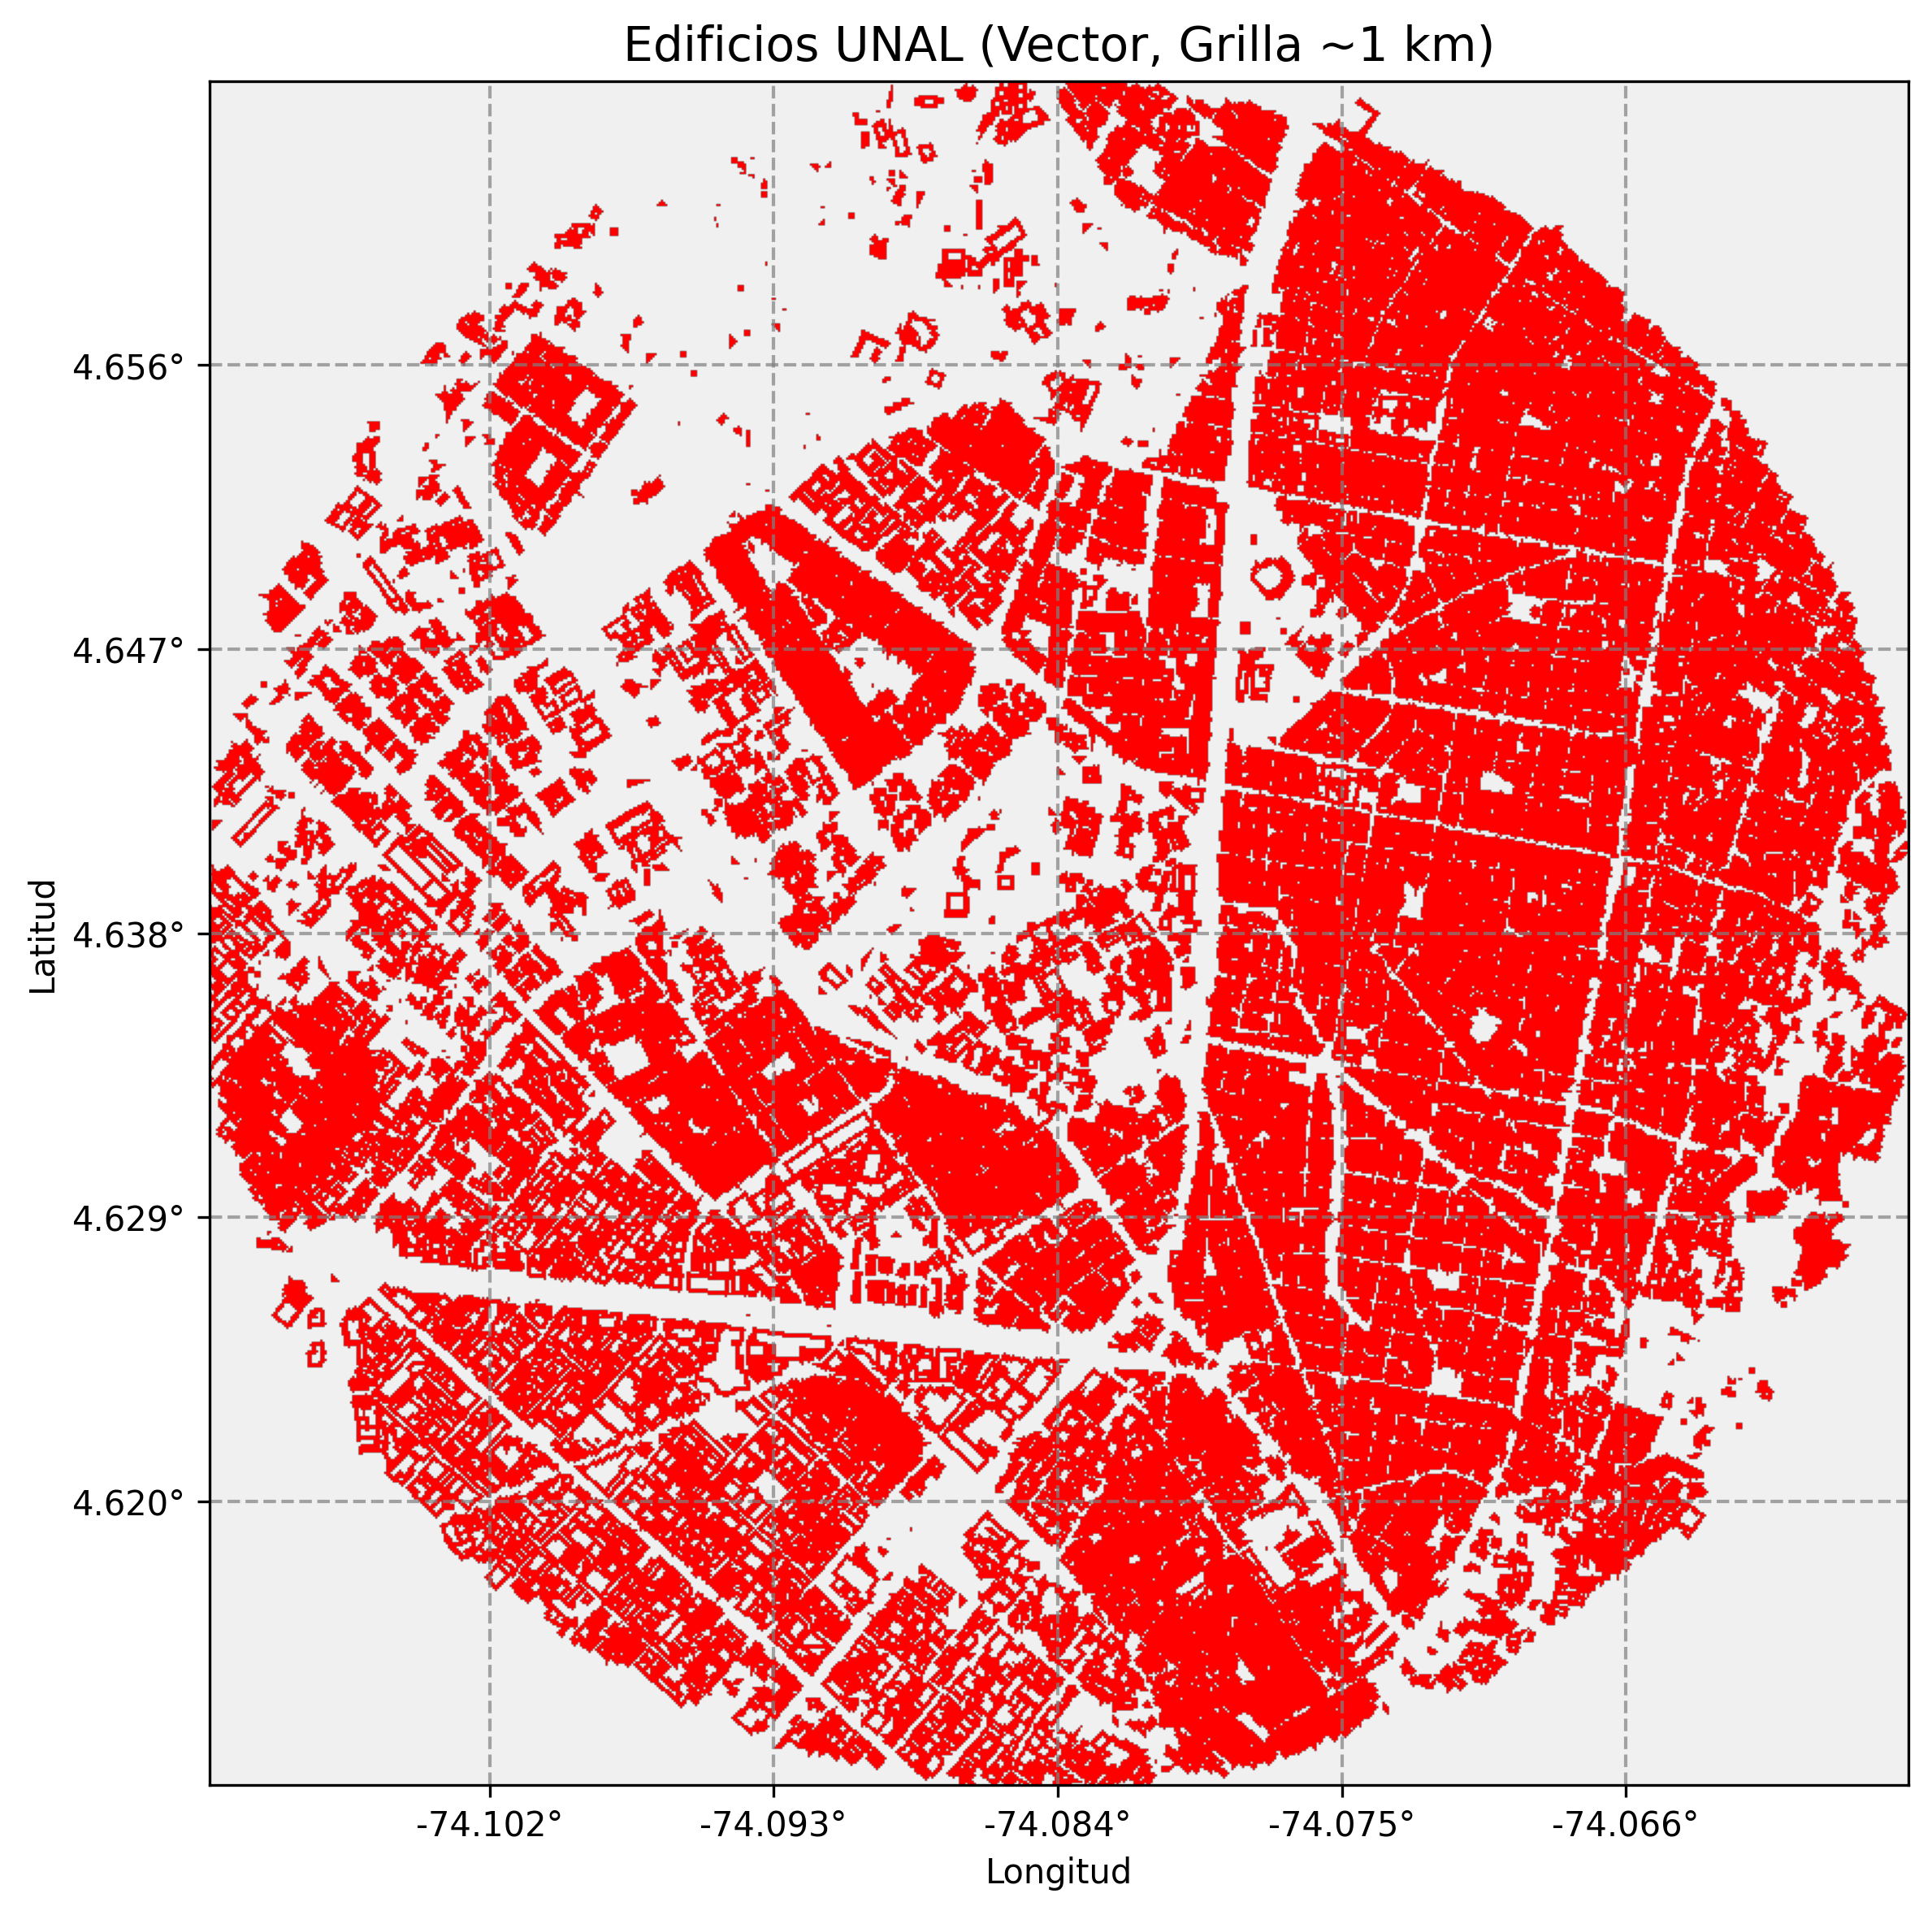
\includegraphics{45-practica_5_clase6_introduccion_sr_gee_files/figure-pdf/fig-python_bld_estatico-output-1.png}

}

\caption{\label{fig-python_bld_estatico}Mapa estático de huellas de
edificios (Open Buildings) con cuadrícula de referencia espacial de 1x1
km.}

\end{figure}%

\subsection{Javascript}

Para ejecutar este código, debes abrir el
\textbf{\href{https://code.earthengine.google.com/}{Code Editor de
Google Earth Engine}} en tu navegador, pegar el siguiente fragmento en
la consola central y hacer clic en \textbf{``Run''}.

\phantomsection\label{js_bld}%
\begin{Shaded}
\begin{Highlighting}[]
\CommentTok{// 1. DEFINICIÓN DEL PUNTO GEOGRÁFICO}
\KeywordTok{var}\NormalTok{ punto\_unal }\OperatorTok{=}\NormalTok{ ee}\OperatorTok{.}\AttributeTok{Geometry}\OperatorTok{.}\FunctionTok{Point}\NormalTok{([}\OperatorTok{{-}}\FloatTok{74.084}\OperatorTok{,} \FloatTok{4.638}\NormalTok{])}\OperatorTok{;}

\CommentTok{// 2. CENTRAR EL VISOR}
\BuiltInTok{Map}\OperatorTok{.}\FunctionTok{centerObject}\NormalTok{(punto\_unal}\OperatorTok{,} \DecValTok{17}\NormalTok{)}\OperatorTok{;}
\BuiltInTok{Map}\OperatorTok{.}\FunctionTok{setOptions}\NormalTok{(}\StringTok{\textquotesingle{}SATELLITE\textquotesingle{}}\NormalTok{)}\OperatorTok{;}

\CommentTok{// 3. CONSULTA DE DATOS VECTORIALES}
\KeywordTok{var}\NormalTok{ buildings }\OperatorTok{=}\NormalTok{ ee}\OperatorTok{.}\FunctionTok{FeatureCollection}\NormalTok{(}\StringTok{"GOOGLE/Research/open{-}buildings/v3/polygons"}\NormalTok{)}\OperatorTok{;}

\CommentTok{// 4. PARÁMETROS DE VISUALIZACIÓN}
\KeywordTok{var}\NormalTok{ visParams }\OperatorTok{=}\NormalTok{ \{}\DataTypeTok{color}\OperatorTok{:} \StringTok{\textquotesingle{}FF0000\textquotesingle{}}\NormalTok{\}}\OperatorTok{;}

\CommentTok{// 5. MOSTRAR EN PANTALLA Y EN CONSOLA}
\BuiltInTok{Map}\OperatorTok{.}\FunctionTok{addLayer}\NormalTok{(buildings}\OperatorTok{,}\NormalTok{ visParams}\OperatorTok{,} \StringTok{\textquotesingle{}Edificios UNAL Bogotá\textquotesingle{}}\NormalTok{)}\OperatorTok{;}

\FunctionTok{print}\NormalTok{(}\StringTok{\textquotesingle{}Metadatos de la colección vectorial (Muestra de 1 elemento):\textquotesingle{}}\OperatorTok{,}\NormalTok{ buildings}\OperatorTok{.}\FunctionTok{limit}\NormalTok{(}\DecValTok{1}\NormalTok{))}\OperatorTok{;}
\FunctionTok{print}\NormalTok{(}\StringTok{\textquotesingle{}ID exacto de la colección:\textquotesingle{}}\OperatorTok{,} \StringTok{\textquotesingle{}GOOGLE/Research/open{-}buildings/v3/polygons\textquotesingle{}}\NormalTok{)}\OperatorTok{;}
\end{Highlighting}
\end{Shaded}

\begin{center}\rule{0.5\linewidth}{0.5pt}\end{center}

\phantomsection\label{js_bld_estatico}%
\begin{Shaded}
\begin{Highlighting}[]
\CommentTok{// ▷ CÓDIGO MAPA ESTÁTICO (THUMBNAIL) EN JAVASCRIPT (Independiente)}

\CommentTok{// 1. DEFINICIÓN DEL PUNTO Y REGIÓN DE INTERÉS}
\KeywordTok{var}\NormalTok{ punto\_unal }\OperatorTok{=}\NormalTok{ ee}\OperatorTok{.}\AttributeTok{Geometry}\OperatorTok{.}\FunctionTok{Point}\NormalTok{([}\OperatorTok{{-}}\FloatTok{74.084}\OperatorTok{,} \FloatTok{4.638}\NormalTok{])}\OperatorTok{;}
\KeywordTok{var}\NormalTok{ region\_interes }\OperatorTok{=}\NormalTok{ punto\_unal}\OperatorTok{.}\FunctionTok{buffer}\NormalTok{(}\DecValTok{3000}\NormalTok{)}\OperatorTok{;} 

\CommentTok{// 2. CONSULTA Y PROCESAMIENTO DE LA IMAGEN (VECTOR A RASTER)}
\KeywordTok{var}\NormalTok{ buildings }\OperatorTok{=}\NormalTok{ ee}\OperatorTok{.}\FunctionTok{FeatureCollection}\NormalTok{(}\StringTok{"GOOGLE/Research/open{-}buildings/v3/polygons"}\NormalTok{)}
  \OperatorTok{.}\FunctionTok{filterBounds}\NormalTok{(region\_interes)}\OperatorTok{;}
  
\KeywordTok{var}\NormalTok{ imagen\_vacia }\OperatorTok{=}\NormalTok{ ee}\OperatorTok{.}\FunctionTok{Image}\NormalTok{()}\OperatorTok{.}\FunctionTok{byte}\NormalTok{()}\OperatorTok{;}
\KeywordTok{var}\NormalTok{ edificios\_raster }\OperatorTok{=}\NormalTok{ imagen\_vacia}\OperatorTok{.}\FunctionTok{paint}\NormalTok{(buildings}\OperatorTok{,} \DecValTok{1}\OperatorTok{,} \DecValTok{2}\NormalTok{)}\OperatorTok{;}

\CommentTok{// 3. PARÁMETROS DE VISUALIZACIÓN}
\KeywordTok{var}\NormalTok{ visParamsEstatica }\OperatorTok{=}\NormalTok{ \{}
  \DataTypeTok{palette}\OperatorTok{:}\NormalTok{ [}\StringTok{\textquotesingle{}red\textquotesingle{}}\NormalTok{]}\OperatorTok{,}
  \DataTypeTok{min}\OperatorTok{:} \DecValTok{1}\OperatorTok{,}
  \DataTypeTok{max}\OperatorTok{:} \DecValTok{1}\OperatorTok{,}
  \DataTypeTok{dimensions}\OperatorTok{:} \DecValTok{800}\OperatorTok{,}
  \DataTypeTok{region}\OperatorTok{:}\NormalTok{ region\_interes}\OperatorTok{,}
  \DataTypeTok{format}\OperatorTok{:} \StringTok{\textquotesingle{}png\textquotesingle{}}
\NormalTok{\}}\OperatorTok{;}

\CommentTok{// 4. MOSTRAR EN CONSOLA LA URL Y EL THUMBNAIL}
\FunctionTok{print}\NormalTok{(}\StringTok{\textquotesingle{}URL de la imagen PNG:\textquotesingle{}}\OperatorTok{,}\NormalTok{ edificios\_raster}\OperatorTok{.}\FunctionTok{getThumbURL}\NormalTok{(visParamsEstatica))}\OperatorTok{;}

\KeywordTok{var}\NormalTok{ miniatura }\OperatorTok{=}\NormalTok{ ui}\OperatorTok{.}\FunctionTok{Thumbnail}\NormalTok{(\{}
  \DataTypeTok{image}\OperatorTok{:}\NormalTok{ edificios\_raster}\OperatorTok{,}
  \DataTypeTok{params}\OperatorTok{:}\NormalTok{ visParamsEstatica}\OperatorTok{,}
  \DataTypeTok{style}\OperatorTok{:}\NormalTok{ \{}\DataTypeTok{width}\OperatorTok{:} \StringTok{\textquotesingle{}400px\textquotesingle{}}\OperatorTok{,} \DataTypeTok{height}\OperatorTok{:} \StringTok{\textquotesingle{}400px\textquotesingle{}}\OperatorTok{,} \DataTypeTok{backgroundColor}\OperatorTok{:} \StringTok{\textquotesingle{}\#f0f0f0\textquotesingle{}}\NormalTok{\}}
\NormalTok{\})}\OperatorTok{;}
\FunctionTok{print}\NormalTok{(}\StringTok{\textquotesingle{}Vista previa estática (Edificios UNAL):\textquotesingle{}}\OperatorTok{,}\NormalTok{ miniatura)}\OperatorTok{;}
\end{Highlighting}
\end{Shaded}

\begin{center}\rule{0.5\linewidth}{0.5pt}\end{center}

\subsection{Reto: Carga de datos vectoriales en QGIS y ArcGIS
Pro}\label{reto-carga-de-datos-vectoriales-en-qgis-y-arcgis-pro}

Importe la capa vectorial de huellas de edificios en su software SIG de
escritorio.

\textbf{Instrucciones:}

\begin{enumerate}
\def\labelenumi{\arabic{enumi}.}
\tightlist
\item
  Ejecute el código de Python correspondiente para generar el archivo
  \texttt{buildings\_serializado.json}.
\item
  En \textbf{QGIS}, emplee la pestaña \emph{Load} del plugin de GEE para
  cargar el Asset ID correspondiente a los polígonos. Asegúrese de
  activar un mapa base satelital en su lienzo para verificar la
  alineación espacial.
\item
  En \textbf{ArcGIS Pro}, utilice la herramienta \emph{Add Feature
  Collection to Map} (o equivalente para colecciones serializadas).
\item
  \textbf{Reporte:} Tome las respectivas capturas de pantalla de la
  configuración de la herramienta antes de su ejecución e insértelas
  reemplazando las rutas indicadas a continuación.
\end{enumerate}

\begin{quote}
\textbf{Reporte visual de Open Buildings}

\emph{Captura de QGIS (Pestaña Load):}
\texttt{!{[}Parámetros\ de\ Open\ Buildings\ en\ QGIS{]}(ruta/a/tu/captura\_qgis\_buildings.png)\{fig-align="center"\ width="80\%"\}}

\emph{Captura de ArcGIS Pro (Herramienta utilizada):}
\texttt{!{[}Parámetros\ de\ Open\ Buildings\ en\ ArcGIS\ Pro{]}(ruta/a/tu/captura\_arcgis\_buildings.png)\{fig-align="center"\ width="80\%"\}}
\end{quote}

\section{Catálogo de datos: BlackMarble (luces
nocturnas)}\label{catuxe1logo-de-datos-blackmarble-luces-nocturnas}

Datos de iluminación nocturna global. El sensor VIIRS captura la emisión
lumínica de las ciudades, lo cual es útil para estudios de urbanización,
actividad económica y densidad poblacional.

\begin{longtable}[]{@{}lll@{}}
\toprule\noalign{}
Banda & Resolución & Descripción \\
\midrule\noalign{}
\endhead
\bottomrule\noalign{}
\endlastfoot
avg\_rad & 500m & Radiancia promedio (luces nocturnas) \\
\end{longtable}

\subsection{Python}

\begin{Shaded}
\begin{Highlighting}[]
\CommentTok{\# \#| eval: false}

\CommentTok{\# Código usando Folium!}

\ImportTok{import}\NormalTok{ ee}
\ImportTok{import}\NormalTok{ folium}
\ImportTok{import}\NormalTok{ datetime}
\ImportTok{import}\NormalTok{ json}

\CommentTok{\# 1. DEFINICIÓN DEL PUNTO GEOGRÁFICO}
\NormalTok{unal\_punto }\OperatorTok{=}\NormalTok{ ee.Geometry.Point([}\OperatorTok{{-}}\FloatTok{74.084}\NormalTok{, }\FloatTok{4.638}\NormalTok{])}

\CommentTok{\# 2. EXPLORAR TODAS LAS OPCIONES Y FILTRAR}
\NormalTok{coleccion\_ntl }\OperatorTok{=}\NormalTok{ (ee.ImageCollection(}\StringTok{"NOAA/VIIRS/DNB/MONTHLY\_V1/VCMSLCFG"}\NormalTok{)}
\NormalTok{    .filterBounds(unal\_punto)}
\NormalTok{    .filterDate(}\StringTok{\textquotesingle{}2023{-}01{-}01\textquotesingle{}}\NormalTok{, }\StringTok{\textquotesingle{}2023{-}12{-}31\textquotesingle{}}\NormalTok{))}

\CommentTok{\# 3. SELECCIÓN DEFINITIVA DE LA IMAGEN}
\NormalTok{ntl }\OperatorTok{=}\NormalTok{ ee.Image(coleccion\_ntl.first())}

\CommentTok{\# 4. EXPORTAR LOS ARCHIVOS JSON (METADATOS Y SERIALIZADO)}
\NormalTok{id\_exacto }\OperatorTok{=}\NormalTok{ ntl.get(}\StringTok{\textquotesingle{}system:id\textquotesingle{}}\NormalTok{).getInfo()}
\BuiltInTok{print}\NormalTok{(}\SpecialStringTok{f"}\CharTok{\textbackslash{}n}\SpecialStringTok{ID de la imagen BlackMarble seleccionada: }\SpecialCharTok{\{}\NormalTok{id\_exacto}\SpecialCharTok{\}}\SpecialStringTok{"}\NormalTok{)}

\NormalTok{metadatos\_json }\OperatorTok{=}\NormalTok{ ntl.getInfo()}
\ControlFlowTok{with} \BuiltInTok{open}\NormalTok{(}\StringTok{\textquotesingle{}metadatos\_ntl.json\textquotesingle{}}\NormalTok{, }\StringTok{\textquotesingle{}w\textquotesingle{}}\NormalTok{) }\ImportTok{as}\NormalTok{ archivo:}
\NormalTok{    json.dump(metadatos\_json, archivo, indent}\OperatorTok{=}\DecValTok{4}\NormalTok{)}

\NormalTok{ntl\_limpia }\OperatorTok{=}\NormalTok{ ee.Image(id\_exacto)}
\NormalTok{texto\_json\_serializado }\OperatorTok{=}\NormalTok{ ntl\_limpia.serialize()}
\ControlFlowTok{with} \BuiltInTok{open}\NormalTok{(}\StringTok{\textquotesingle{}ntl\_serializado.json\textquotesingle{}}\NormalTok{, }\StringTok{\textquotesingle{}w\textquotesingle{}}\NormalTok{) }\ImportTok{as}\NormalTok{ archivo:}
\NormalTok{    json.dump(texto\_json\_serializado, archivo)}

\CommentTok{\# 5. PARÁMETROS DE VISUALIZACIÓN}
\NormalTok{vis\_params }\OperatorTok{=}\NormalTok{ \{}\StringTok{\textquotesingle{}bands\textquotesingle{}}\NormalTok{: [}\StringTok{\textquotesingle{}avg\_rad\textquotesingle{}}\NormalTok{], }\StringTok{\textquotesingle{}min\textquotesingle{}}\NormalTok{: }\DecValTok{0}\NormalTok{, }\StringTok{\textquotesingle{}max\textquotesingle{}}\NormalTok{: }\DecValTok{60}\NormalTok{\}}
\NormalTok{map\_id\_dict }\OperatorTok{=}\NormalTok{ ee.Image(ntl).getMapId(vis\_params)}

\CommentTok{\# 6. CONFIGURACIÓN DEL MAPA BASE (Folium)}
\CommentTok{\# Utilizamos un mapa base oscuro para resaltar las luces nocturnas}
\NormalTok{Map\_ntl }\OperatorTok{=}\NormalTok{ folium.Map(location}\OperatorTok{=}\NormalTok{[}\FloatTok{4.638}\NormalTok{, }\OperatorTok{{-}}\FloatTok{74.084}\NormalTok{], zoom\_start}\OperatorTok{=}\DecValTok{17}\NormalTok{, tiles}\OperatorTok{=}\StringTok{\textquotesingle{}CartoDB dark\_matter\textquotesingle{}}\NormalTok{)}

\CommentTok{\# 7. AGREGAR LA IMAGEN AL VISOR}
\NormalTok{fecha\_capa\_ms }\OperatorTok{=}\NormalTok{ ntl.get(}\StringTok{\textquotesingle{}system:time\_start\textquotesingle{}}\NormalTok{).getInfo()}
\NormalTok{fecha\_capa }\OperatorTok{=}\NormalTok{ datetime.datetime.fromtimestamp(fecha\_capa\_ms }\OperatorTok{/} \FloatTok{1000.0}\NormalTok{, datetime.UTC).strftime(}\StringTok{\textquotesingle{}\%Y{-}\%m{-}}\SpecialCharTok{\%d}\StringTok{\textquotesingle{}}\NormalTok{)}

\NormalTok{folium.TileLayer(}
\NormalTok{    tiles}\OperatorTok{=}\NormalTok{map\_id\_dict[}\StringTok{\textquotesingle{}tile\_fetcher\textquotesingle{}}\NormalTok{].url\_format,}
\NormalTok{    attr}\OperatorTok{=}\StringTok{\textquotesingle{}Google Earth Engine\textquotesingle{}}\NormalTok{,}
\NormalTok{    overlay}\OperatorTok{=}\VariableTok{True}\NormalTok{,}
\NormalTok{    name}\OperatorTok{=}\SpecialStringTok{f\textquotesingle{}Luces Nocturnas {-} }\SpecialCharTok{\{}\NormalTok{fecha\_capa}\SpecialCharTok{\}}\SpecialStringTok{\textquotesingle{}}
\NormalTok{).add\_to(Map\_ntl)}

\NormalTok{folium.LayerControl().add\_to(Map\_ntl)}

\CommentTok{\# 8. VISUALIZACIÓN DEL RESULTADO}
\CommentTok{\# Map\_ntl}
\CommentTok{\# from IPython.display import display, HTML}
\CommentTok{\# display(HTML(Map\_ntl.\_repr\_html\_()))}

\ImportTok{from}\NormalTok{ IPython.display }\ImportTok{import}\NormalTok{ IFrame}

\CommentTok{\# Guardamos el mapa aislado en tu carpeta de trabajo}
\NormalTok{Map\_ntl.save(}\StringTok{"mapas/map\_ntl.html"}\NormalTok{)}

\CommentTok{\# Lo incrustamos en el documento Quarto como una página web independiente}
\NormalTok{display(IFrame(src}\OperatorTok{=}\StringTok{"mapas/map\_ntl.html"}\NormalTok{, width}\OperatorTok{=}\StringTok{"100\%"}\NormalTok{, height}\OperatorTok{=}\StringTok{"500px"}\NormalTok{))}
\end{Highlighting}
\end{Shaded}

\begin{verbatim}

ID de la imagen BlackMarble seleccionada: NOAA/VIIRS/DNB/MONTHLY_V1/VCMSLCFG/20230101
\end{verbatim}

\phantomsection\label{python_ntl}
\begin{verbatim}
<IPython.lib.display.IFrame at 0x7ac2a2d2aff0>
\end{verbatim}

\begin{center}\rule{0.5\linewidth}{0.5pt}\end{center}

\begin{Shaded}
\begin{Highlighting}[]
\CommentTok{\# \#| eval: false}

\CommentTok{\# ▷ CÓDIGO MAPA ESTÁTICO (PNG) PARA FOLIUM/GENERAL (Independiente)}
\ImportTok{import}\NormalTok{ ee}
\ImportTok{import}\NormalTok{ requests}
\ImportTok{import}\NormalTok{ matplotlib.pyplot }\ImportTok{as}\NormalTok{ plt}
\ImportTok{from}\NormalTok{ matplotlib.cm }\ImportTok{import}\NormalTok{ ScalarMappable}
\ImportTok{from}\NormalTok{ matplotlib.colors }\ImportTok{import}\NormalTok{ Normalize}
\ImportTok{from}\NormalTok{ PIL }\ImportTok{import}\NormalTok{ Image}
\ImportTok{from}\NormalTok{ io }\ImportTok{import}\NormalTok{ BytesIO}

\CommentTok{\# 1. DEFINICIÓN DEL ÁREA (BOGOTÁ COMPLETA)}
\NormalTok{localidades }\OperatorTok{=}\NormalTok{ ee.FeatureCollection(}\StringTok{"FAO/GAUL/2015/level2"}\NormalTok{)}
\NormalTok{bogota }\OperatorTok{=}\NormalTok{ localidades.}\BuiltInTok{filter}\NormalTok{(ee.Filter.eq(}\StringTok{\textquotesingle{}ADM2\_NAME\textquotesingle{}}\NormalTok{, }\StringTok{\textquotesingle{}Santafe De Bogota D.c.\textquotesingle{}}\NormalTok{))}
\NormalTok{region\_interes }\OperatorTok{=}\NormalTok{ bogota.geometry().bounds()}

\CommentTok{\# 2. CONSULTA Y PROCESAMIENTO DE LA IMAGEN}
\NormalTok{ntl\_estatica }\OperatorTok{=}\NormalTok{ ee.ImageCollection(}\StringTok{"NOAA/VIIRS/DNB/MONTHLY\_V1/VCMSLCFG"}\NormalTok{)}\OperatorTok{\textbackslash{}}
\NormalTok{    .filterBounds(bogota)}\OperatorTok{\textbackslash{}}
\NormalTok{    .filterDate(}\StringTok{\textquotesingle{}2023{-}01{-}01\textquotesingle{}}\NormalTok{, }\StringTok{\textquotesingle{}2023{-}12{-}31\textquotesingle{}}\NormalTok{)}\OperatorTok{\textbackslash{}}
\NormalTok{    .first()}\OperatorTok{\textbackslash{}}
\NormalTok{    .clip(bogota)}

\CommentTok{\# 3. OBTENER LA URL DEL THUMBNAIL DESDE GOOGLE EARTH ENGINE}
\NormalTok{url\_img }\OperatorTok{=}\NormalTok{ ntl\_estatica.getThumbURL(\{}
    \StringTok{\textquotesingle{}bands\textquotesingle{}}\NormalTok{: [}\StringTok{\textquotesingle{}avg\_rad\textquotesingle{}}\NormalTok{],}
    \StringTok{\textquotesingle{}min\textquotesingle{}}\NormalTok{: }\DecValTok{0}\NormalTok{,}
    \StringTok{\textquotesingle{}max\textquotesingle{}}\NormalTok{: }\DecValTok{60}\NormalTok{,}
    \StringTok{\textquotesingle{}palette\textquotesingle{}}\NormalTok{: [}\StringTok{\textquotesingle{}black\textquotesingle{}}\NormalTok{, }\StringTok{\textquotesingle{}white\textquotesingle{}}\NormalTok{],}
    \StringTok{\textquotesingle{}dimensions\textquotesingle{}}\NormalTok{: }\DecValTok{800}\NormalTok{,}
    \StringTok{\textquotesingle{}region\textquotesingle{}}\NormalTok{: region\_interes}
\NormalTok{\})}

\CommentTok{\# 4. DESCARGAR Y DIBUJAR LA IMAGEN CON MATPLOTLIB (Grilla y Leyenda)}
\NormalTok{respuesta }\OperatorTok{=}\NormalTok{ requests.get(url\_img)}
\NormalTok{imagen\_png }\OperatorTok{=}\NormalTok{ Image.}\BuiltInTok{open}\NormalTok{(BytesIO(respuesta.content))}

\CommentTok{\# Coordenadas límite para georreferenciar}
\NormalTok{coords }\OperatorTok{=}\NormalTok{ region\_interes.coordinates().get(}\DecValTok{0}\NormalTok{).getInfo()}
\NormalTok{xmin }\OperatorTok{=} \BuiltInTok{min}\NormalTok{([c[}\DecValTok{0}\NormalTok{] }\ControlFlowTok{for}\NormalTok{ c }\KeywordTok{in}\NormalTok{ coords])}
\NormalTok{xmax }\OperatorTok{=} \BuiltInTok{max}\NormalTok{([c[}\DecValTok{0}\NormalTok{] }\ControlFlowTok{for}\NormalTok{ c }\KeywordTok{in}\NormalTok{ coords])}
\NormalTok{ymin }\OperatorTok{=} \BuiltInTok{min}\NormalTok{([c[}\DecValTok{1}\NormalTok{] }\ControlFlowTok{for}\NormalTok{ c }\KeywordTok{in}\NormalTok{ coords])}
\NormalTok{ymax }\OperatorTok{=} \BuiltInTok{max}\NormalTok{([c[}\DecValTok{1}\NormalTok{] }\ControlFlowTok{for}\NormalTok{ c }\KeywordTok{in}\NormalTok{ coords])}

\NormalTok{fig, ax }\OperatorTok{=}\NormalTok{ plt.subplots(figsize}\OperatorTok{=}\NormalTok{(}\DecValTok{8}\NormalTok{, }\DecValTok{8}\NormalTok{))}

\NormalTok{ax.imshow(imagen\_png, extent}\OperatorTok{=}\NormalTok{[xmin, xmax, ymin, ymax])}

\CommentTok{\# Grilla de 10 km. (1 grado ≈ 111 km {-}\textgreater{} 10 km ≈ 0.09 grados)}
\NormalTok{paso\_10km }\OperatorTok{=} \FloatTok{0.09} 
\NormalTok{lon\_centro, lat\_centro }\OperatorTok{=}\NormalTok{ (xmin }\OperatorTok{+}\NormalTok{ xmax) }\OperatorTok{/} \DecValTok{2}\NormalTok{, (ymin }\OperatorTok{+}\NormalTok{ ymax) }\OperatorTok{/} \DecValTok{2}

\NormalTok{x\_ticks }\OperatorTok{=}\NormalTok{ [lon\_centro }\OperatorTok{+}\NormalTok{ (i }\OperatorTok{*}\NormalTok{ paso\_10km) }\ControlFlowTok{for}\NormalTok{ i }\KeywordTok{in} \BuiltInTok{range}\NormalTok{(}\OperatorTok{{-}}\DecValTok{5}\NormalTok{, }\DecValTok{6}\NormalTok{)]}
\NormalTok{y\_ticks }\OperatorTok{=}\NormalTok{ [lat\_centro }\OperatorTok{+}\NormalTok{ (i }\OperatorTok{*}\NormalTok{ paso\_10km) }\ControlFlowTok{for}\NormalTok{ i }\KeywordTok{in} \BuiltInTok{range}\NormalTok{(}\OperatorTok{{-}}\DecValTok{5}\NormalTok{, }\DecValTok{6}\NormalTok{)]}

\NormalTok{x\_ticks }\OperatorTok{=}\NormalTok{ [x }\ControlFlowTok{for}\NormalTok{ x }\KeywordTok{in}\NormalTok{ x\_ticks }\ControlFlowTok{if}\NormalTok{ xmin }\OperatorTok{\textless{}=}\NormalTok{ x }\OperatorTok{\textless{}=}\NormalTok{ xmax]}
\NormalTok{y\_ticks }\OperatorTok{=}\NormalTok{ [y }\ControlFlowTok{for}\NormalTok{ y }\KeywordTok{in}\NormalTok{ y\_ticks }\ControlFlowTok{if}\NormalTok{ ymin }\OperatorTok{\textless{}=}\NormalTok{ y }\OperatorTok{\textless{}=}\NormalTok{ ymax]}

\NormalTok{ax.set\_xticks(x\_ticks)}
\NormalTok{ax.set\_yticks(y\_ticks)}
\NormalTok{ax.set\_xticklabels([}\SpecialStringTok{f"}\SpecialCharTok{\{}\NormalTok{x}\SpecialCharTok{:.2f\}}\SpecialStringTok{°"} \ControlFlowTok{for}\NormalTok{ x }\KeywordTok{in}\NormalTok{ x\_ticks])}
\NormalTok{ax.set\_yticklabels([}\SpecialStringTok{f"}\SpecialCharTok{\{}\NormalTok{y}\SpecialCharTok{:.2f\}}\SpecialStringTok{°"} \ControlFlowTok{for}\NormalTok{ y }\KeywordTok{in}\NormalTok{ y\_ticks])}

\NormalTok{ax.grid(color}\OperatorTok{=}\StringTok{\textquotesingle{}white\textquotesingle{}}\NormalTok{, linestyle}\OperatorTok{=}\StringTok{\textquotesingle{}{-}{-}\textquotesingle{}}\NormalTok{, linewidth}\OperatorTok{=}\FloatTok{0.8}\NormalTok{, alpha}\OperatorTok{=}\FloatTok{0.5}\NormalTok{)}
\NormalTok{ax.set\_title(}\StringTok{\textquotesingle{}Luces Nocturnas VIIRS {-} Bogotá (Píxel \textasciitilde{}500 m, Grilla \textasciitilde{}10 km)\textquotesingle{}}\NormalTok{, fontsize}\OperatorTok{=}\DecValTok{14}\NormalTok{)}
\NormalTok{ax.set\_xlabel(}\StringTok{\textquotesingle{}Longitud\textquotesingle{}}\NormalTok{)}
\NormalTok{ax.set\_ylabel(}\StringTok{\textquotesingle{}Latitud\textquotesingle{}}\NormalTok{)}
\NormalTok{ax.set\_facecolor(}\StringTok{\textquotesingle{}\#202020\textquotesingle{}}\NormalTok{)}

\CommentTok{\# 5. AGREGAR LEYENDA (COLORBAR) CON UNIDADES}
\NormalTok{norm }\OperatorTok{=}\NormalTok{ Normalize(vmin}\OperatorTok{=}\DecValTok{0}\NormalTok{, vmax}\OperatorTok{=}\DecValTok{60}\NormalTok{)}
\NormalTok{cbar }\OperatorTok{=}\NormalTok{ fig.colorbar(ScalarMappable(norm}\OperatorTok{=}\NormalTok{norm, cmap}\OperatorTok{=}\StringTok{\textquotesingle{}gray\textquotesingle{}}\NormalTok{), ax}\OperatorTok{=}\NormalTok{ax, shrink}\OperatorTok{=}\FloatTok{0.75}\NormalTok{, pad}\OperatorTok{=}\FloatTok{0.04}\NormalTok{)}
\NormalTok{cbar.set\_label(}\StringTok{\textquotesingle{}Radiancia (nW/cm²/sr)\textquotesingle{}}\NormalTok{, rotation}\OperatorTok{=}\DecValTok{270}\NormalTok{, labelpad}\OperatorTok{=}\DecValTok{15}\NormalTok{)}

\NormalTok{plt.tight\_layout()}
\NormalTok{plt.show()}
\end{Highlighting}
\end{Shaded}

\begin{figure}[H]

\centering{

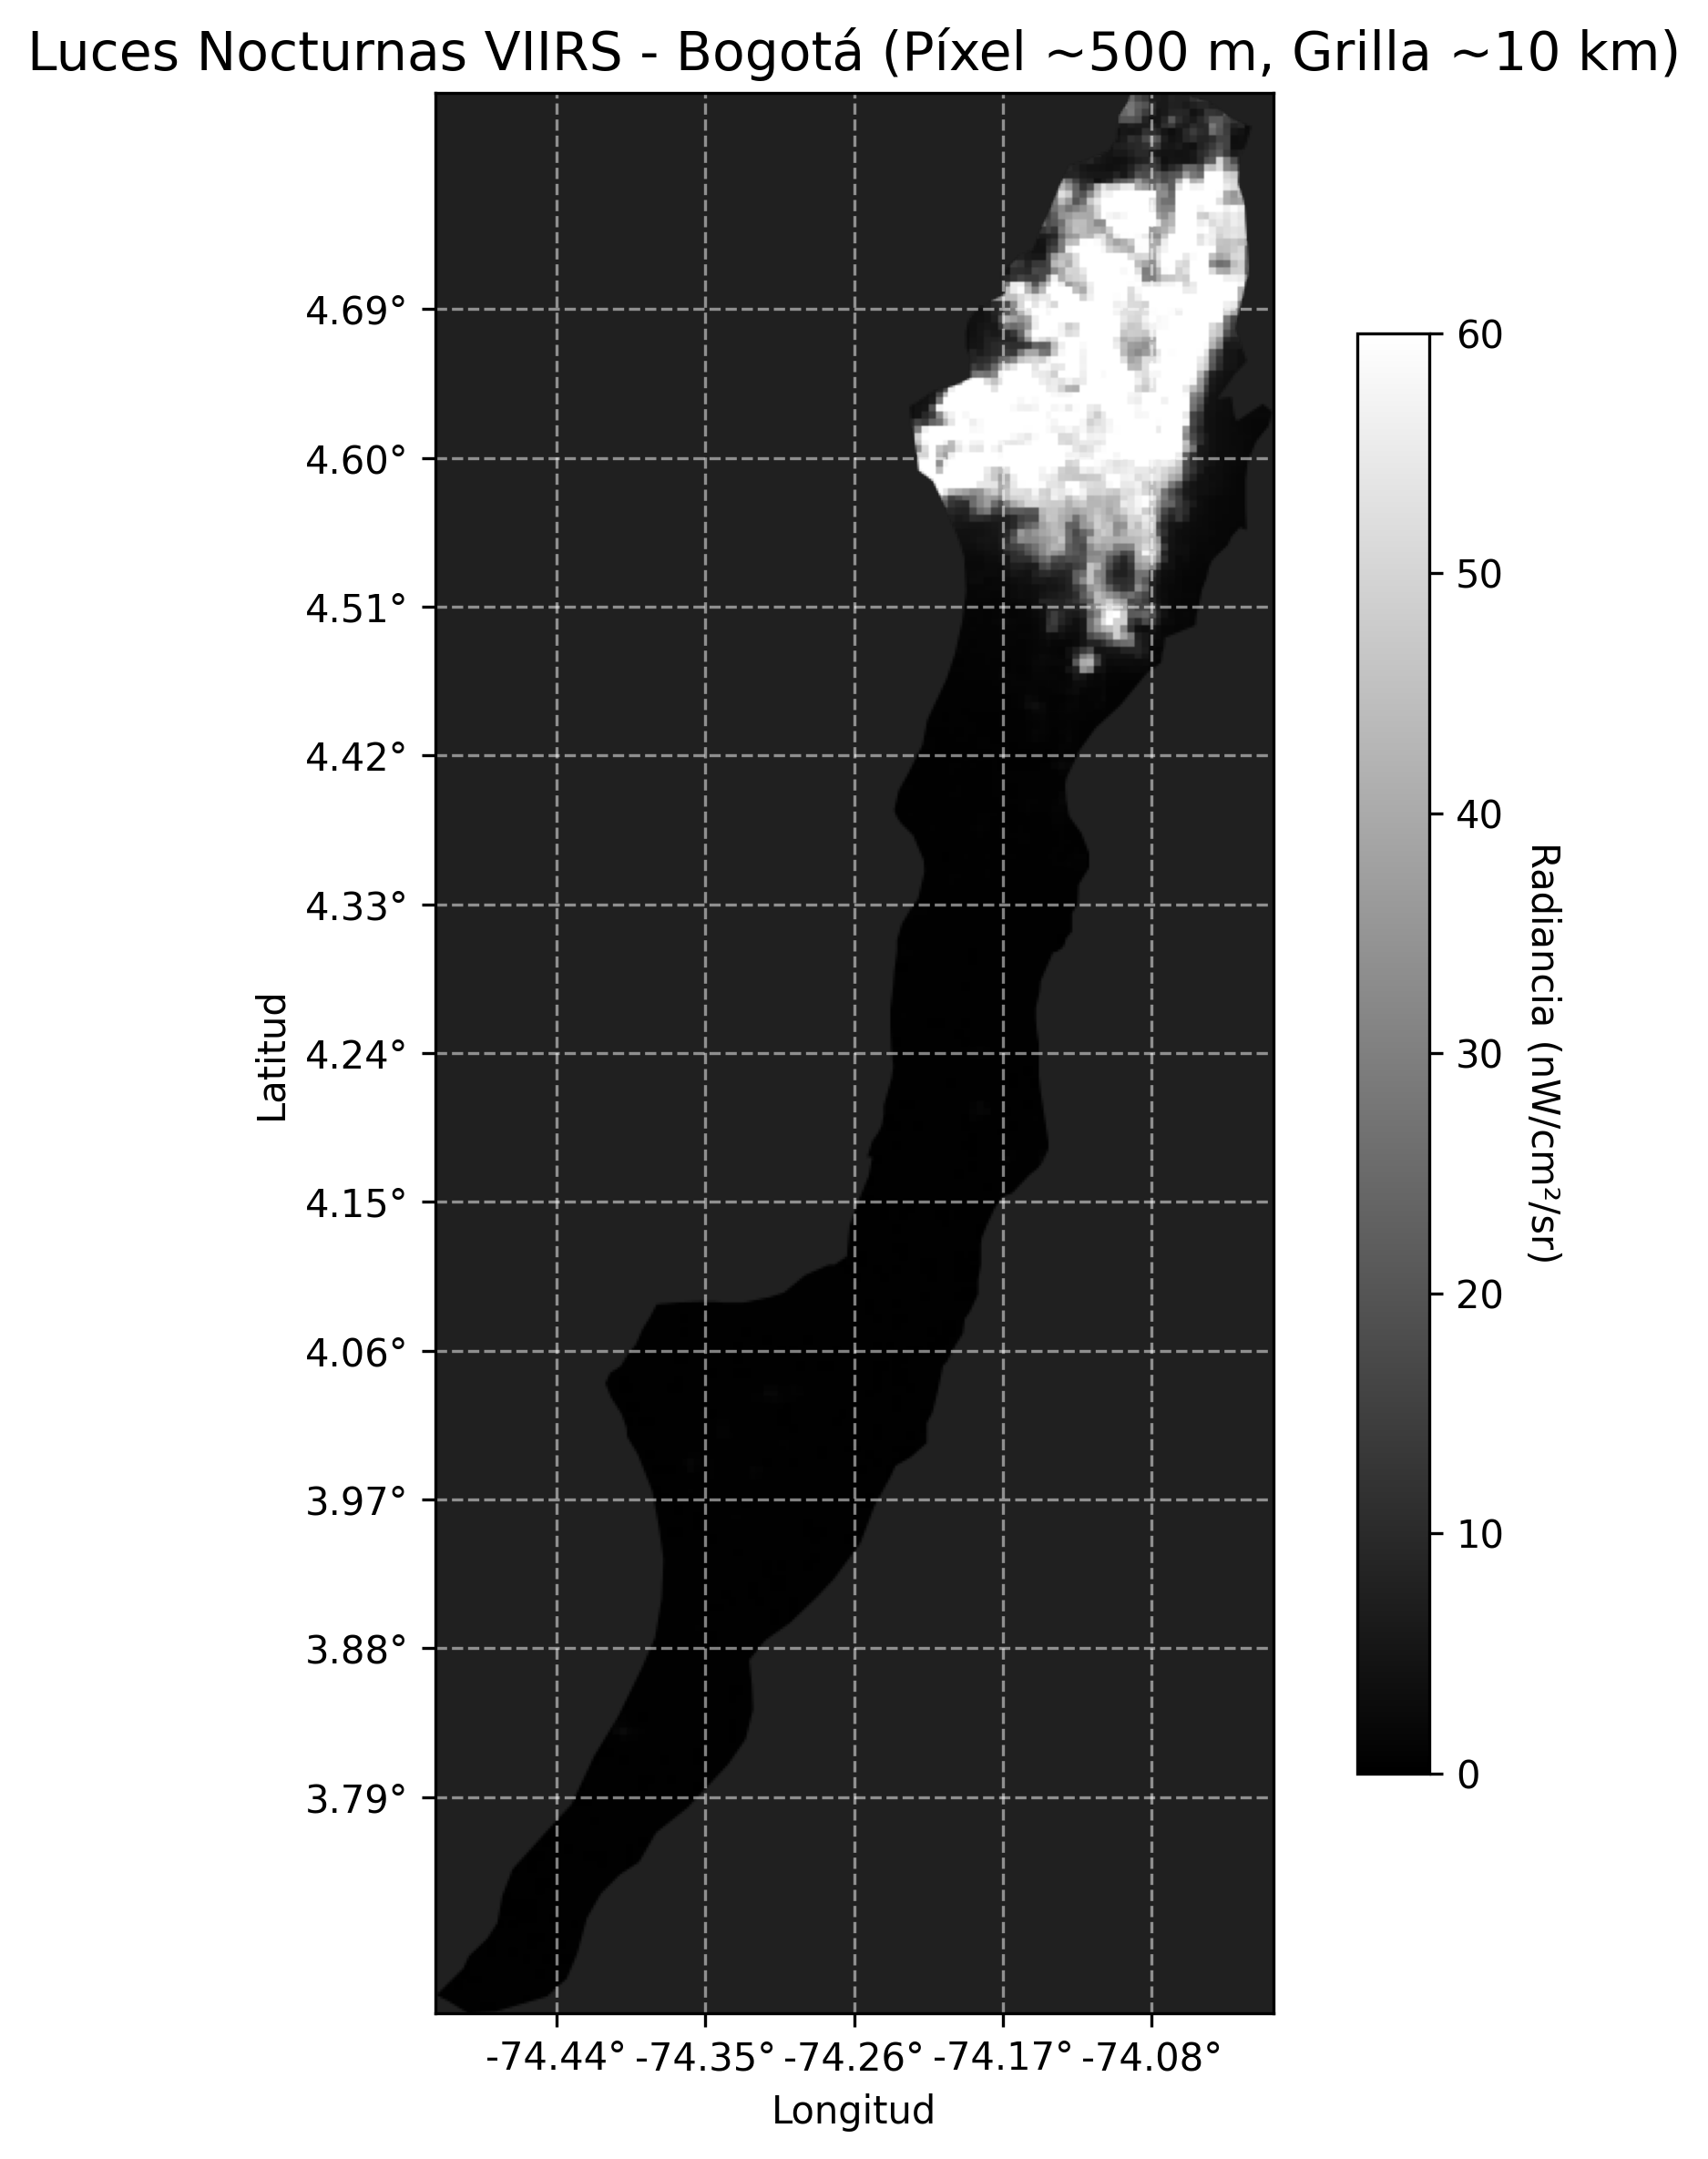
\includegraphics{45-practica_5_clase6_introduccion_sr_gee_files/figure-pdf/fig-python_ntl_estatico-output-1.png}

}

\caption{\label{fig-python_ntl_estatico}Mapa estático de luces nocturnas
(BlackMarble/VIIRS) para la ciudad de Bogotá D.C., con leyenda de
radiancia y grilla de referencia.}

\end{figure}%

\subsection{Javascript}

Para ejecutar este código, debes abrir el
\textbf{\href{https://code.earthengine.google.com/}{Code Editor de
Google Earth Engine}} en tu navegador, pegar el siguiente fragmento en
la consola central y hacer clic en \textbf{``Run''}.

\phantomsection\label{js_ntl}%
\begin{Shaded}
\begin{Highlighting}[]
\CommentTok{// 1. DEFINICIÓN DEL PUNTO GEOGRÁFICO}
\KeywordTok{var}\NormalTok{ punto\_unal }\OperatorTok{=}\NormalTok{ ee}\OperatorTok{.}\AttributeTok{Geometry}\OperatorTok{.}\FunctionTok{Point}\NormalTok{([}\OperatorTok{{-}}\FloatTok{74.084}\OperatorTok{,} \FloatTok{4.638}\NormalTok{])}\OperatorTok{;}

\CommentTok{// 2. CENTRAR EL VISOR}
\BuiltInTok{Map}\OperatorTok{.}\FunctionTok{centerObject}\NormalTok{(punto\_unal}\OperatorTok{,} \DecValTok{17}\NormalTok{)}\OperatorTok{;}

\CommentTok{// 3. CONSULTA Y FILTRADO DE DATOS}
\KeywordTok{var}\NormalTok{ ntl }\OperatorTok{=}\NormalTok{ ee}\OperatorTok{.}\FunctionTok{ImageCollection}\NormalTok{(}\StringTok{"NOAA/VIIRS/DNB/MONTHLY\_V1/VCMSLCFG"}\NormalTok{)}
  \OperatorTok{.}\FunctionTok{filterBounds}\NormalTok{(punto\_unal)}
  \OperatorTok{.}\FunctionTok{filterDate}\NormalTok{(}\StringTok{\textquotesingle{}2023{-}01{-}01\textquotesingle{}}\OperatorTok{,} \StringTok{\textquotesingle{}2023{-}12{-}31\textquotesingle{}}\NormalTok{)}
  \OperatorTok{.}\FunctionTok{first}\NormalTok{()}\OperatorTok{;}

\CommentTok{// 4. PARÁMETROS DE VISUALIZACIÓN}
\KeywordTok{var}\NormalTok{ visParams }\OperatorTok{=}\NormalTok{ \{}\DataTypeTok{bands}\OperatorTok{:}\NormalTok{ [}\StringTok{\textquotesingle{}avg\_rad\textquotesingle{}}\NormalTok{]}\OperatorTok{,} \DataTypeTok{min}\OperatorTok{:} \DecValTok{0}\OperatorTok{,} \DataTypeTok{max}\OperatorTok{:} \DecValTok{60}\NormalTok{\}}\OperatorTok{;}

\CommentTok{// 5. MOSTRAR EN PANTALLA Y EN CONSOLA}
\BuiltInTok{Map}\OperatorTok{.}\FunctionTok{addLayer}\NormalTok{(ntl}\OperatorTok{,}\NormalTok{ visParams}\OperatorTok{,} \StringTok{\textquotesingle{}Luces Nocturnas {-} UNAL Bogotá\textquotesingle{}}\NormalTok{)}\OperatorTok{;}

\FunctionTok{print}\NormalTok{(}\StringTok{\textquotesingle{}Metadatos de la imagen BlackMarble:\textquotesingle{}}\OperatorTok{,}\NormalTok{ ntl)}\OperatorTok{;}
\FunctionTok{print}\NormalTok{(}\StringTok{\textquotesingle{}ID exacto de la imagen BlackMarble:\textquotesingle{}}\OperatorTok{,}\NormalTok{ ntl}\OperatorTok{.}\FunctionTok{get}\NormalTok{(}\StringTok{\textquotesingle{}system:id\textquotesingle{}}\NormalTok{))}\OperatorTok{;}
\end{Highlighting}
\end{Shaded}

\begin{center}\rule{0.5\linewidth}{0.5pt}\end{center}

\phantomsection\label{js_ntl_estatico}%
\begin{Shaded}
\begin{Highlighting}[]
\CommentTok{// ▷ CÓDIGO MAPA ESTÁTICO (THUMBNAIL) EN JAVASCRIPT (Independiente)}

\CommentTok{// 1. DEFINICIÓN DEL ÁREA (BOGOTÁ COMPLETA)}
\KeywordTok{var}\NormalTok{ localidades }\OperatorTok{=}\NormalTok{ ee}\OperatorTok{.}\FunctionTok{FeatureCollection}\NormalTok{(}\StringTok{"FAO/GAUL/2015/level2"}\NormalTok{)}\OperatorTok{;}
\KeywordTok{var}\NormalTok{ bogota }\OperatorTok{=}\NormalTok{ localidades}\OperatorTok{.}\FunctionTok{filter}\NormalTok{(ee}\OperatorTok{.}\AttributeTok{Filter}\OperatorTok{.}\FunctionTok{eq}\NormalTok{(}\StringTok{\textquotesingle{}ADM2\_NAME\textquotesingle{}}\OperatorTok{,} \StringTok{\textquotesingle{}Santafe De Bogota D.c.\textquotesingle{}}\NormalTok{))}\OperatorTok{;}
\KeywordTok{var}\NormalTok{ region\_interes }\OperatorTok{=}\NormalTok{ bogota}\OperatorTok{.}\FunctionTok{geometry}\NormalTok{()}\OperatorTok{.}\FunctionTok{bounds}\NormalTok{()}\OperatorTok{;}

\CommentTok{// 2. CONSULTA Y PROCESAMIENTO DE LA IMAGEN}
\KeywordTok{var}\NormalTok{ ntl\_estatica }\OperatorTok{=}\NormalTok{ ee}\OperatorTok{.}\FunctionTok{ImageCollection}\NormalTok{(}\StringTok{"NOAA/VIIRS/DNB/MONTHLY\_V1/VCMSLCFG"}\NormalTok{)}
  \OperatorTok{.}\FunctionTok{filterBounds}\NormalTok{(bogota)}
  \OperatorTok{.}\FunctionTok{filterDate}\NormalTok{(}\StringTok{\textquotesingle{}2023{-}01{-}01\textquotesingle{}}\OperatorTok{,} \StringTok{\textquotesingle{}2023{-}12{-}31\textquotesingle{}}\NormalTok{)}
  \OperatorTok{.}\FunctionTok{first}\NormalTok{()}
  \OperatorTok{.}\FunctionTok{clip}\NormalTok{(bogota)}\OperatorTok{;}

\CommentTok{// 3. PARÁMETROS DE VISUALIZACIÓN}
\KeywordTok{var}\NormalTok{ visParamsEstatica }\OperatorTok{=}\NormalTok{ \{}
  \DataTypeTok{bands}\OperatorTok{:}\NormalTok{ [}\StringTok{\textquotesingle{}avg\_rad\textquotesingle{}}\NormalTok{]}\OperatorTok{,}
  \DataTypeTok{min}\OperatorTok{:} \DecValTok{0}\OperatorTok{,}
  \DataTypeTok{max}\OperatorTok{:} \DecValTok{60}\OperatorTok{,}
  \DataTypeTok{palette}\OperatorTok{:}\NormalTok{ [}\StringTok{\textquotesingle{}black\textquotesingle{}}\OperatorTok{,} \StringTok{\textquotesingle{}white\textquotesingle{}}\NormalTok{]}\OperatorTok{,}
  \DataTypeTok{dimensions}\OperatorTok{:} \DecValTok{800}\OperatorTok{,}
  \DataTypeTok{region}\OperatorTok{:}\NormalTok{ region\_interes}
\NormalTok{\}}\OperatorTok{;}

\CommentTok{// 4. MOSTRAR EN CONSOLA LA URL Y EL THUMBNAIL}
\FunctionTok{print}\NormalTok{(}\StringTok{\textquotesingle{}URL de la imagen PNG:\textquotesingle{}}\OperatorTok{,}\NormalTok{ ntl\_estatica}\OperatorTok{.}\FunctionTok{getThumbURL}\NormalTok{(visParamsEstatica))}\OperatorTok{;}

\KeywordTok{var}\NormalTok{ miniatura }\OperatorTok{=}\NormalTok{ ui}\OperatorTok{.}\FunctionTok{Thumbnail}\NormalTok{(\{}
  \DataTypeTok{image}\OperatorTok{:}\NormalTok{ ntl\_estatica}\OperatorTok{,}
  \DataTypeTok{params}\OperatorTok{:}\NormalTok{ visParamsEstatica}\OperatorTok{,}
  \DataTypeTok{style}\OperatorTok{:}\NormalTok{ \{}\DataTypeTok{width}\OperatorTok{:} \StringTok{\textquotesingle{}400px\textquotesingle{}}\OperatorTok{,} \DataTypeTok{height}\OperatorTok{:} \StringTok{\textquotesingle{}400px\textquotesingle{}}\OperatorTok{,} \DataTypeTok{backgroundColor}\OperatorTok{:} \StringTok{\textquotesingle{}\#202020\textquotesingle{}}\NormalTok{\}}
\NormalTok{\})}\OperatorTok{;}
\FunctionTok{print}\NormalTok{(}\StringTok{\textquotesingle{}Vista previa estática (Luces Nocturnas {-} Bogotá):\textquotesingle{}}\OperatorTok{,}\NormalTok{ miniatura)}\OperatorTok{;}
\end{Highlighting}
\end{Shaded}

\begin{center}\rule{0.5\linewidth}{0.5pt}\end{center}

\subsection{Reto: Carga de imagen nocturna en QGIS y ArcGIS
Pro}\label{reto-carga-de-imagen-nocturna-en-qgis-y-arcgis-pro}

Proceda a importar la imagen de luces nocturnas en su entorno SIG de
escritorio.

\textbf{Instrucciones:}

\begin{enumerate}
\def\labelenumi{\arabic{enumi}.}
\tightlist
\item
  Ejecute el código de Python correspondiente para generar el archivo
  \texttt{ntl\_serializado.json}.
\item
  En \textbf{QGIS}, emplee la pestaña \emph{Load} del plugin de GEE para
  cargar el Asset ID. Especifique la banda \texttt{avg\_rad} y los
  valores mínimo (\texttt{0}) y máximo (\texttt{60}).
\item
  En \textbf{ArcGIS Pro}, utilice la herramienta \emph{Add Image to Map
  by Serialized Object} o su equivalente mediante Asset ID.
\item
  \textbf{Reporte:} Capture la pantalla de la herramienta configurada
  antes de su ejecución e insértela a continuación.
\end{enumerate}

\begin{quote}
\textbf{Reporte visual de BlackMarble}

\emph{Captura de QGIS (Pestaña Load):}
\texttt{!{[}Parámetros\ de\ BlackMarble\ en\ QGIS{]}(ruta/a/tu/captura\_qgis\_ntl.png)\{fig-align="center"\ width="80\%"\}}

\emph{Captura de ArcGIS Pro (Herramienta utilizada):}
\texttt{!{[}Parámetros\ de\ BlackMarble\ en\ ArcGIS\ Pro{]}(ruta/a/tu/captura\_arcgis\_ntl.png)\{fig-align="center"\ width="80\%"\}}
\end{quote}

\begin{center}\rule{0.5\linewidth}{0.5pt}\end{center}

\section{Catálogo de datos: DSWx Sentinel-1 (cuerpos de
agua)}\label{catuxe1logo-de-datos-dswx-sentinel-1-cuerpos-de-agua}

Datos de detección de agua superficial. Este producto utiliza imágenes
de radar de Sentinel-1 para clasificar cuerpos de agua, siendo
resistente a la cobertura de nubes.

\begin{longtable}[]{@{}lll@{}}
\toprule\noalign{}
Banda & Resolución & Descripción \\
\midrule\noalign{}
\endhead
\bottomrule\noalign{}
\endlastfoot
WTR\_Water\_classification & 30m & Clasificación de agua (OPERA) \\
\end{longtable}

\subsection{Python}

\begin{Shaded}
\begin{Highlighting}[]
\CommentTok{\# \#| eval: false}

\CommentTok{\# Código usando Folium!}

\ImportTok{import}\NormalTok{ ee}
\ImportTok{import}\NormalTok{ folium}
\ImportTok{import}\NormalTok{ json}

\CommentTok{\# 1. DEFINICIÓN DEL PUNTO GEOGRÁFICO}
\NormalTok{unal\_punto }\OperatorTok{=}\NormalTok{ ee.Geometry.Point([}\OperatorTok{{-}}\FloatTok{74.084}\NormalTok{, }\FloatTok{4.638}\NormalTok{])}

\CommentTok{\# 2. EXPLORAR TODAS LAS OPCIONES Y FILTRAR}
\NormalTok{coleccion\_dswx }\OperatorTok{=}\NormalTok{ ee.ImageCollection(}\StringTok{"OPERA/DSWX/L3\_V1/S1"}\NormalTok{).filterBounds(unal\_punto)}

\CommentTok{\# 3. SELECCIÓN DEFINITIVA DE LA IMAGEN}
\NormalTok{dswx }\OperatorTok{=}\NormalTok{ ee.Image(coleccion\_dswx.first())}

\CommentTok{\# 4. EXPORTAR LOS ARCHIVOS JSON (METADATOS Y SERIALIZADO)}
\NormalTok{id\_exacto }\OperatorTok{=}\NormalTok{ dswx.get(}\StringTok{\textquotesingle{}system:id\textquotesingle{}}\NormalTok{).getInfo()}
\BuiltInTok{print}\NormalTok{(}\SpecialStringTok{f"}\CharTok{\textbackslash{}n}\SpecialStringTok{ID de la imagen DSWx seleccionada: }\SpecialCharTok{\{}\NormalTok{id\_exacto}\SpecialCharTok{\}}\SpecialStringTok{"}\NormalTok{)}

\NormalTok{metadatos\_json }\OperatorTok{=}\NormalTok{ dswx.getInfo()}
\ControlFlowTok{with} \BuiltInTok{open}\NormalTok{(}\StringTok{\textquotesingle{}metadatos\_dswx.json\textquotesingle{}}\NormalTok{, }\StringTok{\textquotesingle{}w\textquotesingle{}}\NormalTok{) }\ImportTok{as}\NormalTok{ archivo:}
\NormalTok{    json.dump(metadatos\_json, archivo, indent}\OperatorTok{=}\DecValTok{4}\NormalTok{)}

\NormalTok{dswx\_limpia }\OperatorTok{=}\NormalTok{ ee.Image(id\_exacto)}
\NormalTok{texto\_json\_serializado }\OperatorTok{=}\NormalTok{ dswx\_limpia.serialize()}
\ControlFlowTok{with} \BuiltInTok{open}\NormalTok{(}\StringTok{\textquotesingle{}dswx\_serializado.json\textquotesingle{}}\NormalTok{, }\StringTok{\textquotesingle{}w\textquotesingle{}}\NormalTok{) }\ImportTok{as}\NormalTok{ archivo:}
\NormalTok{    json.dump(texto\_json\_serializado, archivo)}

\CommentTok{\# 5. PARÁMETROS DE VISUALIZACIÓN}
\NormalTok{vis\_params }\OperatorTok{=}\NormalTok{ \{}
    \StringTok{\textquotesingle{}bands\textquotesingle{}}\NormalTok{: [}\StringTok{\textquotesingle{}WTR\_Water\_classification\textquotesingle{}}\NormalTok{], }
    \StringTok{\textquotesingle{}min\textquotesingle{}}\NormalTok{: }\DecValTok{0}\NormalTok{, }
    \StringTok{\textquotesingle{}max\textquotesingle{}}\NormalTok{: }\DecValTok{4}\NormalTok{, }
    \StringTok{\textquotesingle{}palette\textquotesingle{}}\NormalTok{: [}\StringTok{\textquotesingle{}white\textquotesingle{}}\NormalTok{, }\StringTok{\textquotesingle{}blue\textquotesingle{}}\NormalTok{, }\StringTok{\textquotesingle{}cyan\textquotesingle{}}\NormalTok{, }\StringTok{\textquotesingle{}gray\textquotesingle{}}\NormalTok{, }\StringTok{\textquotesingle{}black\textquotesingle{}}\NormalTok{]}
\NormalTok{\}}
\NormalTok{map\_id\_dict }\OperatorTok{=}\NormalTok{ ee.Image(dswx).getMapId(vis\_params)}

\CommentTok{\# 6. CONFIGURACIÓN DEL MAPA BASE (Folium)}
\NormalTok{Map\_dswx }\OperatorTok{=}\NormalTok{ folium.Map(location}\OperatorTok{=}\NormalTok{[}\FloatTok{4.638}\NormalTok{, }\OperatorTok{{-}}\FloatTok{74.084}\NormalTok{], zoom\_start}\OperatorTok{=}\DecValTok{17}\NormalTok{)}

\CommentTok{\# 7. AGREGAR LA IMAGEN AL VISOR}
\NormalTok{folium.TileLayer(}
\NormalTok{    tiles}\OperatorTok{=}\NormalTok{map\_id\_dict[}\StringTok{\textquotesingle{}tile\_fetcher\textquotesingle{}}\NormalTok{].url\_format,}
\NormalTok{    attr}\OperatorTok{=}\StringTok{\textquotesingle{}Google Earth Engine\textquotesingle{}}\NormalTok{,}
\NormalTok{    overlay}\OperatorTok{=}\VariableTok{True}\NormalTok{,}
\NormalTok{    name}\OperatorTok{=}\StringTok{\textquotesingle{}DSWx Agua\textquotesingle{}}
\NormalTok{).add\_to(Map\_dswx)}

\NormalTok{folium.LayerControl().add\_to(Map\_dswx)}

\CommentTok{\# 8. VISUALIZACIÓN DEL RESULTADO}
\CommentTok{\# Map\_dswx}
\CommentTok{\# from IPython.display import display, HTML}
\CommentTok{\# display(HTML(Map\_dswx.\_repr\_html\_()))}

\ImportTok{from}\NormalTok{ IPython.display }\ImportTok{import}\NormalTok{ IFrame}

\CommentTok{\# Guardamos el mapa aislado en tu carpeta de trabajo}
\NormalTok{Map\_dswx.save(}\StringTok{"mapas/map\_dswx.html"}\NormalTok{)}

\CommentTok{\# Lo incrustamos en el documento Quarto como una página web independiente}
\NormalTok{display(IFrame(src}\OperatorTok{=}\StringTok{"mapas/map\_dswx.html"}\NormalTok{, width}\OperatorTok{=}\StringTok{"100\%"}\NormalTok{, height}\OperatorTok{=}\StringTok{"500px"}\NormalTok{))}
\end{Highlighting}
\end{Shaded}

\begin{verbatim}

ID de la imagen DSWx seleccionada: OPERA/DSWX/L3_V1/S1/T18NWL_20240830T104323Z_20251107T024246Z_S1A
\end{verbatim}

\phantomsection\label{python_dswx}
\begin{verbatim}
<IPython.lib.display.IFrame at 0x7ac2a2f89b20>
\end{verbatim}

\begin{center}\rule{0.5\linewidth}{0.5pt}\end{center}

\begin{Shaded}
\begin{Highlighting}[]
\CommentTok{\# \#| eval: false}

\CommentTok{\# ▷ CÓDIGO MAPA ESTÁTICO (PNG) PARA FOLIUM/GENERAL (Independiente)}
\ImportTok{import}\NormalTok{ ee}
\ImportTok{import}\NormalTok{ requests}
\ImportTok{import}\NormalTok{ matplotlib.pyplot }\ImportTok{as}\NormalTok{ plt}
\ImportTok{import}\NormalTok{ matplotlib.patches }\ImportTok{as}\NormalTok{ mpatches}
\ImportTok{from}\NormalTok{ PIL }\ImportTok{import}\NormalTok{ Image}
\ImportTok{from}\NormalTok{ io }\ImportTok{import}\NormalTok{ BytesIO}

\CommentTok{\# 1. DEFINICIÓN DEL PUNTO GEOGRÁFICO Y REGIÓN DE INTERÉS}
\NormalTok{lon\_centro, lat\_centro }\OperatorTok{=} \OperatorTok{{-}}\FloatTok{74.084}\NormalTok{, }\FloatTok{4.638}
\NormalTok{unal\_punto }\OperatorTok{=}\NormalTok{ ee.Geometry.Point([lon\_centro, lat\_centro])}
\NormalTok{region\_interes }\OperatorTok{=}\NormalTok{ unal\_punto.}\BuiltInTok{buffer}\NormalTok{(}\DecValTok{3000}\NormalTok{) }

\CommentTok{\# 2. CONSULTA Y PROCESAMIENTO DE LA IMAGEN}
\NormalTok{dswx\_estatica }\OperatorTok{=}\NormalTok{ ee.ImageCollection(}\StringTok{"OPERA/DSWX/L3\_V1/S1"}\NormalTok{)}\OperatorTok{\textbackslash{}}
\NormalTok{    .filterBounds(unal\_punto)}\OperatorTok{\textbackslash{}}
\NormalTok{    .first()}

\CommentTok{\# 3. OBTENER LA URL DEL THUMBNAIL DESDE GOOGLE EARTH ENGINE}
\NormalTok{url\_img }\OperatorTok{=}\NormalTok{ dswx\_estatica.getThumbURL(\{}
    \StringTok{\textquotesingle{}bands\textquotesingle{}}\NormalTok{: [}\StringTok{\textquotesingle{}WTR\_Water\_classification\textquotesingle{}}\NormalTok{],}
    \StringTok{\textquotesingle{}min\textquotesingle{}}\NormalTok{: }\DecValTok{0}\NormalTok{,}
    \StringTok{\textquotesingle{}max\textquotesingle{}}\NormalTok{: }\DecValTok{4}\NormalTok{,}
    \StringTok{\textquotesingle{}palette\textquotesingle{}}\NormalTok{: [}\StringTok{\textquotesingle{}white\textquotesingle{}}\NormalTok{, }\StringTok{\textquotesingle{}blue\textquotesingle{}}\NormalTok{, }\StringTok{\textquotesingle{}cyan\textquotesingle{}}\NormalTok{, }\StringTok{\textquotesingle{}gray\textquotesingle{}}\NormalTok{, }\StringTok{\textquotesingle{}black\textquotesingle{}}\NormalTok{],}
    \StringTok{\textquotesingle{}dimensions\textquotesingle{}}\NormalTok{: }\DecValTok{800}\NormalTok{,}
    \StringTok{\textquotesingle{}region\textquotesingle{}}\NormalTok{: region\_interes}
\NormalTok{\})}

\CommentTok{\# 4. DESCARGAR Y DIBUJAR LA IMAGEN CON MATPLOTLIB (Grilla y Leyenda)}
\NormalTok{respuesta }\OperatorTok{=}\NormalTok{ requests.get(url\_img)}
\NormalTok{imagen\_png }\OperatorTok{=}\NormalTok{ Image.}\BuiltInTok{open}\NormalTok{(BytesIO(respuesta.content))}

\NormalTok{coords }\OperatorTok{=}\NormalTok{ region\_interes.bounds().coordinates().get(}\DecValTok{0}\NormalTok{).getInfo()}
\NormalTok{xmin, ymin }\OperatorTok{=}\NormalTok{ coords[}\DecValTok{0}\NormalTok{][}\DecValTok{0}\NormalTok{], coords[}\DecValTok{0}\NormalTok{][}\DecValTok{1}\NormalTok{]}
\NormalTok{xmax, ymax }\OperatorTok{=}\NormalTok{ coords[}\DecValTok{2}\NormalTok{][}\DecValTok{0}\NormalTok{], coords[}\DecValTok{2}\NormalTok{][}\DecValTok{1}\NormalTok{]}

\NormalTok{fig, ax }\OperatorTok{=}\NormalTok{ plt.subplots(figsize}\OperatorTok{=}\NormalTok{(}\DecValTok{10}\NormalTok{, }\DecValTok{8}\NormalTok{)) }

\NormalTok{ax.imshow(imagen\_png, extent}\OperatorTok{=}\NormalTok{[xmin, xmax, ymin, ymax])}

\CommentTok{\# Grilla de 1 km. (1 grado ≈ 111 km {-}\textgreater{} 1 km ≈ 0.009 grados)}
\NormalTok{paso\_1km }\OperatorTok{=} \FloatTok{0.009} 
\NormalTok{x\_ticks }\OperatorTok{=}\NormalTok{ [lon\_centro }\OperatorTok{+}\NormalTok{ (i }\OperatorTok{*}\NormalTok{ paso\_1km) }\ControlFlowTok{for}\NormalTok{ i }\KeywordTok{in} \BuiltInTok{range}\NormalTok{(}\OperatorTok{{-}}\DecValTok{4}\NormalTok{, }\DecValTok{5}\NormalTok{)]}
\NormalTok{y\_ticks }\OperatorTok{=}\NormalTok{ [lat\_centro }\OperatorTok{+}\NormalTok{ (i }\OperatorTok{*}\NormalTok{ paso\_1km) }\ControlFlowTok{for}\NormalTok{ i }\KeywordTok{in} \BuiltInTok{range}\NormalTok{(}\OperatorTok{{-}}\DecValTok{4}\NormalTok{, }\DecValTok{5}\NormalTok{)]}

\NormalTok{x\_ticks }\OperatorTok{=}\NormalTok{ [x }\ControlFlowTok{for}\NormalTok{ x }\KeywordTok{in}\NormalTok{ x\_ticks }\ControlFlowTok{if}\NormalTok{ xmin }\OperatorTok{\textless{}=}\NormalTok{ x }\OperatorTok{\textless{}=}\NormalTok{ xmax]}
\NormalTok{y\_ticks }\OperatorTok{=}\NormalTok{ [y }\ControlFlowTok{for}\NormalTok{ y }\KeywordTok{in}\NormalTok{ y\_ticks }\ControlFlowTok{if}\NormalTok{ ymin }\OperatorTok{\textless{}=}\NormalTok{ y }\OperatorTok{\textless{}=}\NormalTok{ ymax]}

\NormalTok{ax.set\_xticks(x\_ticks)}
\NormalTok{ax.set\_yticks(y\_ticks)}
\NormalTok{ax.set\_xticklabels([}\SpecialStringTok{f"}\SpecialCharTok{\{}\NormalTok{x}\SpecialCharTok{:.3f\}}\SpecialStringTok{°"} \ControlFlowTok{for}\NormalTok{ x }\KeywordTok{in}\NormalTok{ x\_ticks])}
\NormalTok{ax.set\_yticklabels([}\SpecialStringTok{f"}\SpecialCharTok{\{}\NormalTok{y}\SpecialCharTok{:.3f\}}\SpecialStringTok{°"} \ControlFlowTok{for}\NormalTok{ y }\KeywordTok{in}\NormalTok{ y\_ticks])}

\NormalTok{ax.grid(color}\OperatorTok{=}\StringTok{\textquotesingle{}gray\textquotesingle{}}\NormalTok{, linestyle}\OperatorTok{=}\StringTok{\textquotesingle{}{-}{-}\textquotesingle{}}\NormalTok{, linewidth}\OperatorTok{=}\DecValTok{1}\NormalTok{, alpha}\OperatorTok{=}\FloatTok{0.7}\NormalTok{)}
\NormalTok{ax.set\_title(}\StringTok{\textquotesingle{}Clasificación de Agua DSWx (Píxel \textasciitilde{}30 m, Grilla \textasciitilde{}1 km)\textquotesingle{}}\NormalTok{, fontsize}\OperatorTok{=}\DecValTok{14}\NormalTok{)}
\NormalTok{ax.set\_xlabel(}\StringTok{\textquotesingle{}Longitud\textquotesingle{}}\NormalTok{)}
\NormalTok{ax.set\_ylabel(}\StringTok{\textquotesingle{}Latitud\textquotesingle{}}\NormalTok{)}

\CommentTok{\# 5. AGREGAR LEYENDA CATEGÓRICA}
\NormalTok{colores }\OperatorTok{=}\NormalTok{ [}\StringTok{\textquotesingle{}white\textquotesingle{}}\NormalTok{, }\StringTok{\textquotesingle{}blue\textquotesingle{}}\NormalTok{, }\StringTok{\textquotesingle{}cyan\textquotesingle{}}\NormalTok{, }\StringTok{\textquotesingle{}gray\textquotesingle{}}\NormalTok{, }\StringTok{\textquotesingle{}black\textquotesingle{}}\NormalTok{]}
\NormalTok{etiquetas }\OperatorTok{=}\NormalTok{ [}
    \StringTok{\textquotesingle{}0: No Agua\textquotesingle{}}\NormalTok{, }
    \StringTok{\textquotesingle{}1: Agua Abierta\textquotesingle{}}\NormalTok{, }
    \StringTok{\textquotesingle{}2: Agua Parcial\textquotesingle{}}\NormalTok{, }
    \StringTok{\textquotesingle{}3: Nieve / Hielo\textquotesingle{}}\NormalTok{, }
    \StringTok{\textquotesingle{}4: Sombra / Nubes\textquotesingle{}}
\NormalTok{]}

\NormalTok{parches }\OperatorTok{=}\NormalTok{ [mpatches.Patch(color}\OperatorTok{=}\NormalTok{colores[i], label}\OperatorTok{=}\NormalTok{etiquetas[i], ec}\OperatorTok{=}\StringTok{\textquotesingle{}black\textquotesingle{}}\NormalTok{) }\ControlFlowTok{for}\NormalTok{ i }\KeywordTok{in} \BuiltInTok{range}\NormalTok{(}\BuiltInTok{len}\NormalTok{(colores))]}
\NormalTok{ax.legend(handles}\OperatorTok{=}\NormalTok{parches, bbox\_to\_anchor}\OperatorTok{=}\NormalTok{(}\FloatTok{1.05}\NormalTok{, }\DecValTok{1}\NormalTok{), loc}\OperatorTok{=}\StringTok{\textquotesingle{}upper left\textquotesingle{}}\NormalTok{, title}\OperatorTok{=}\StringTok{"Clases DSWx"}\NormalTok{, frameon}\OperatorTok{=}\VariableTok{True}\NormalTok{)}

\NormalTok{plt.tight\_layout()}
\NormalTok{plt.show()}
\end{Highlighting}
\end{Shaded}

\begin{figure}[H]

\centering{

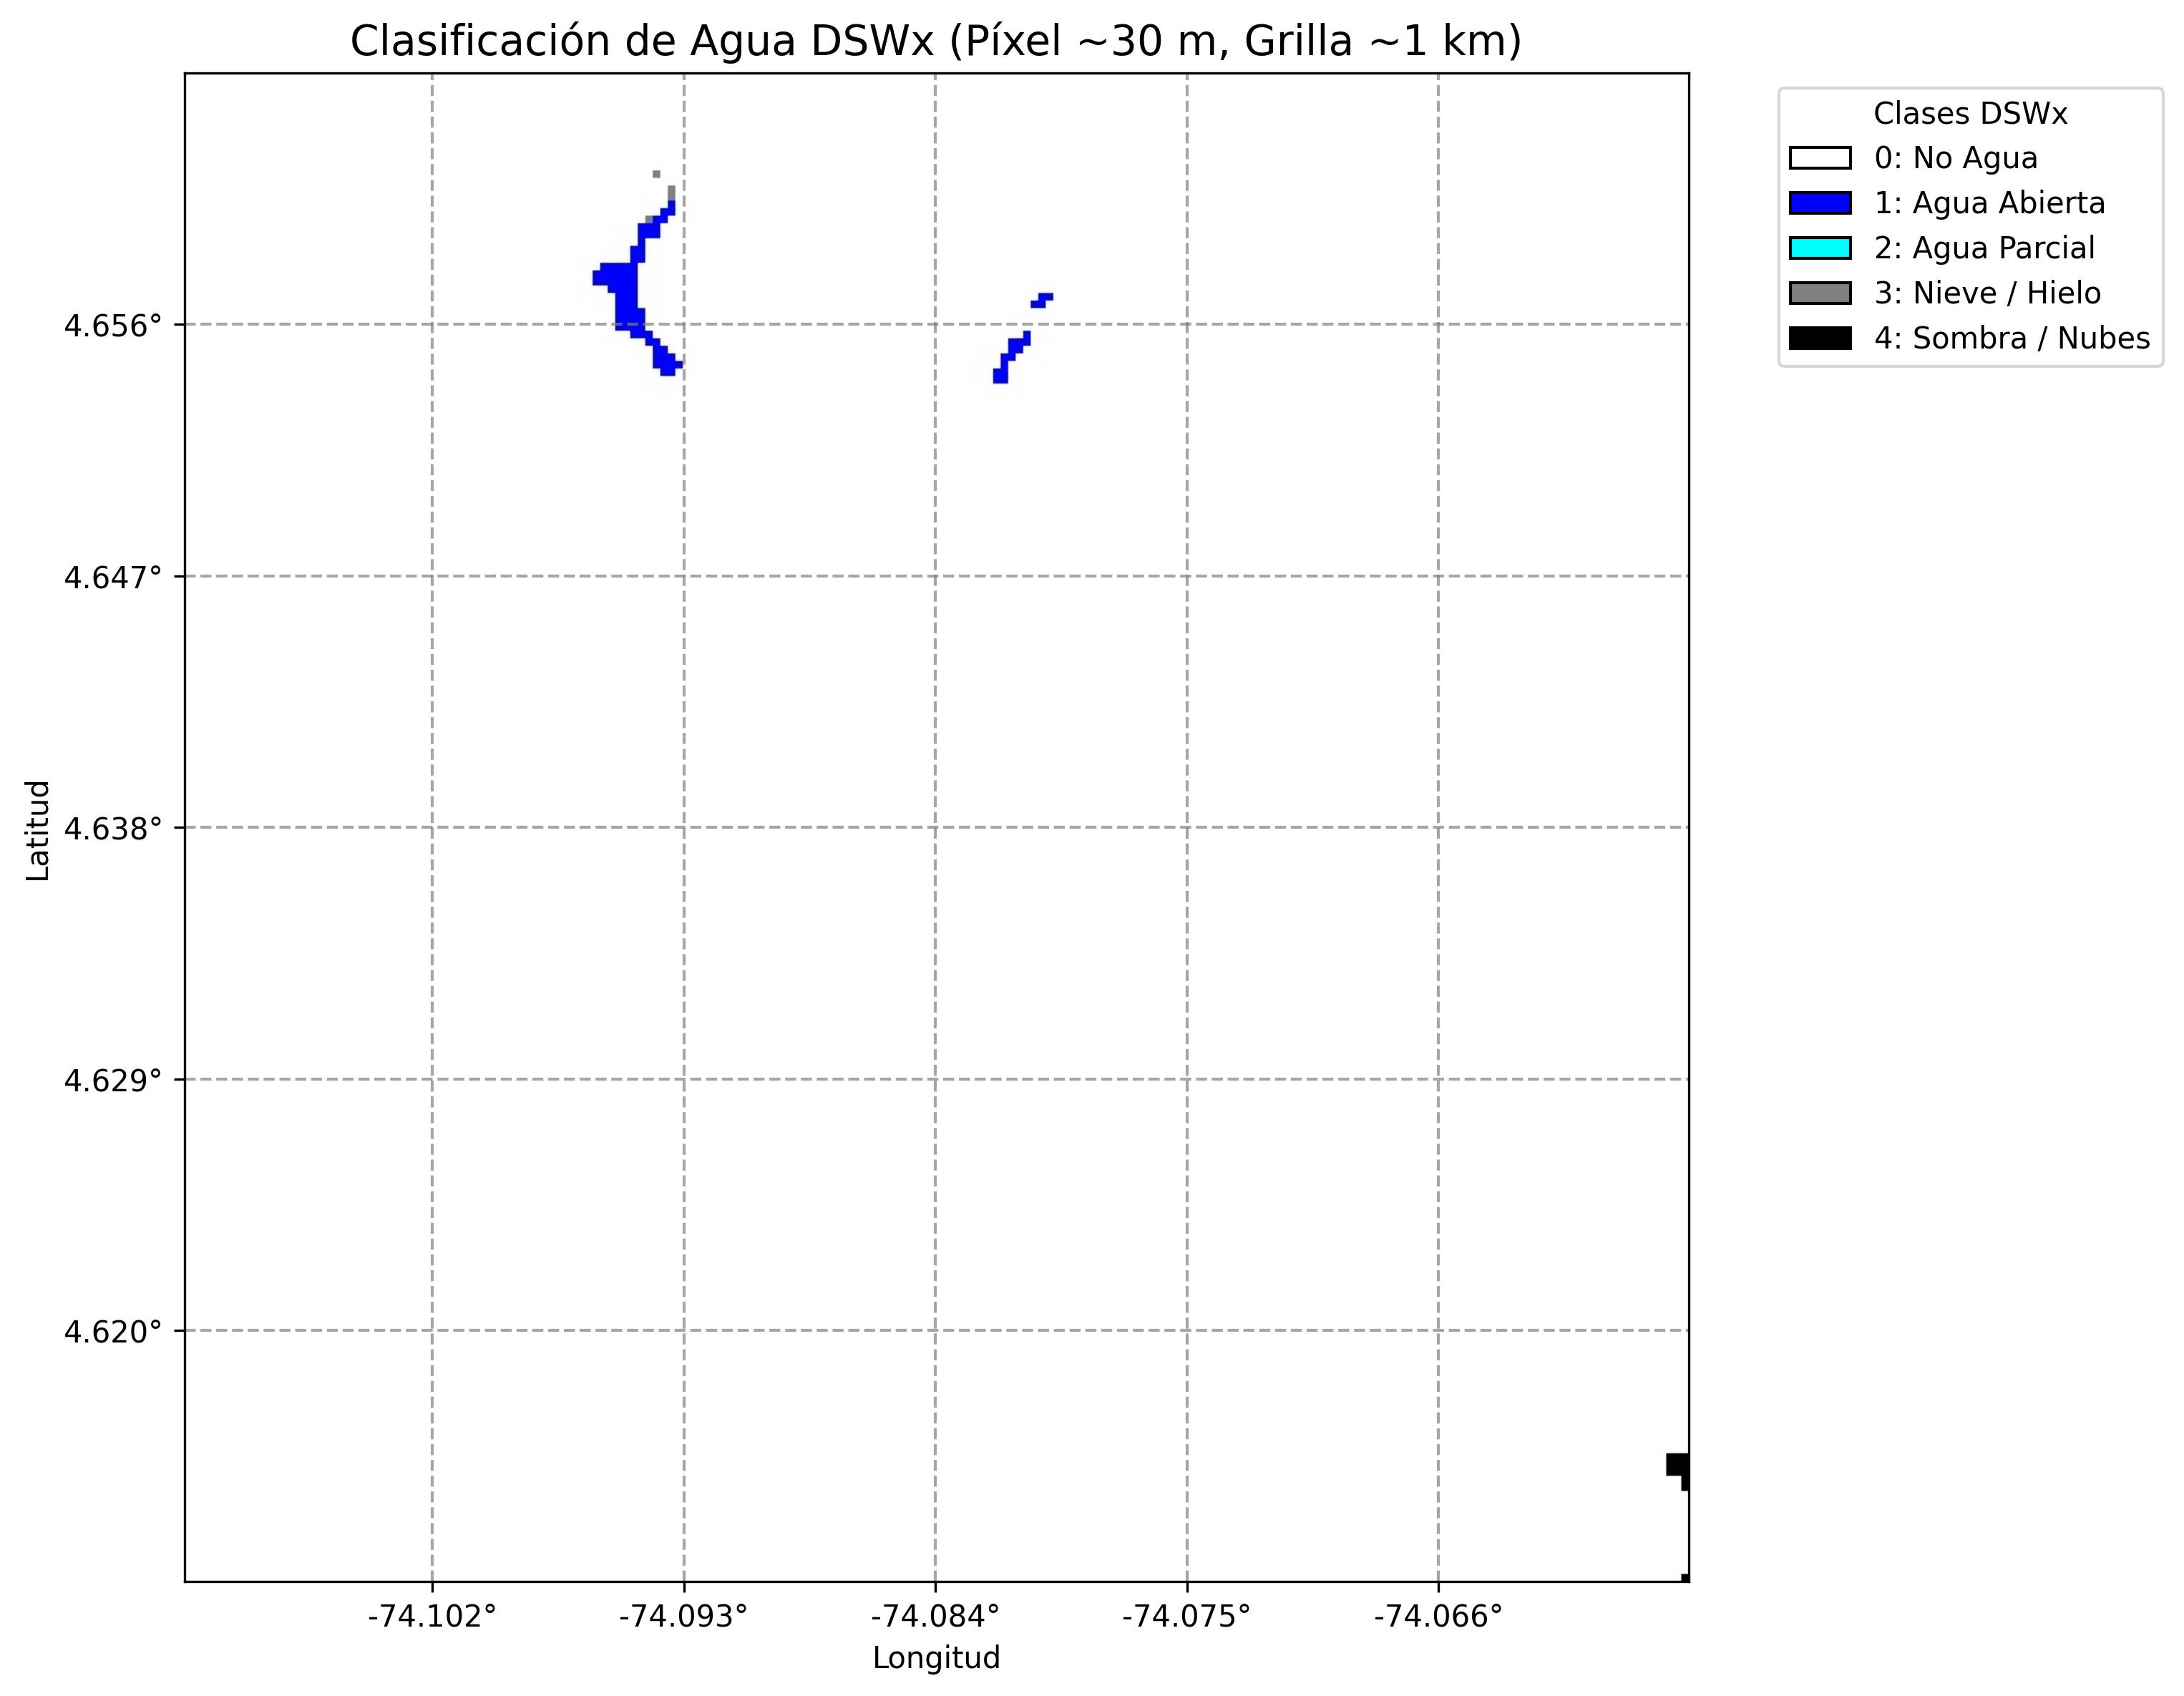
\includegraphics{45-practica_5_clase6_introduccion_sr_gee_files/figure-pdf/fig-python_dswx_estatico-output-1.png}

}

\caption{\label{fig-python_dswx_estatico}Mapa estático de clasificación
de agua (DSWx) con leyenda categórica y grilla espacial.}

\end{figure}%

\subsection{Javascript}

Para ejecutar este código, debes abrir el
\textbf{\href{https://code.earthengine.google.com/}{Code Editor de
Google Earth Engine}} en tu navegador, pegar el siguiente fragmento en
la consola central y hacer clic en \textbf{``Run''}.

\phantomsection\label{js_dswx}%
\begin{Shaded}
\begin{Highlighting}[]
\CommentTok{// 1. DEFINICIÓN DEL PUNTO GEOGRÁFICO}
\KeywordTok{var}\NormalTok{ punto\_unal }\OperatorTok{=}\NormalTok{ ee}\OperatorTok{.}\AttributeTok{Geometry}\OperatorTok{.}\FunctionTok{Point}\NormalTok{([}\OperatorTok{{-}}\FloatTok{74.084}\OperatorTok{,} \FloatTok{4.638}\NormalTok{])}\OperatorTok{;}

\CommentTok{// 2. CENTRAR EL VISOR}
\BuiltInTok{Map}\OperatorTok{.}\FunctionTok{centerObject}\NormalTok{(punto\_unal}\OperatorTok{,} \DecValTok{17}\NormalTok{)}\OperatorTok{;}

\CommentTok{// 3. CONSULTA Y FILTRADO DE DATOS}
\KeywordTok{var}\NormalTok{ dswx }\OperatorTok{=}\NormalTok{ ee}\OperatorTok{.}\FunctionTok{ImageCollection}\NormalTok{(}\StringTok{"OPERA/DSWX/L3\_V1/S1"}\NormalTok{)}\OperatorTok{.}\FunctionTok{filterBounds}\NormalTok{(punto\_unal)}\OperatorTok{.}\FunctionTok{first}\NormalTok{()}\OperatorTok{;}

\CommentTok{// 4. PARÁMETROS DE VISUALIZACIÓN}
\KeywordTok{var}\NormalTok{ visParams }\OperatorTok{=}\NormalTok{ \{}
  \DataTypeTok{bands}\OperatorTok{:}\NormalTok{ [}\StringTok{\textquotesingle{}WTR\_Water\_classification\textquotesingle{}}\NormalTok{]}\OperatorTok{,} 
  \DataTypeTok{min}\OperatorTok{:} \DecValTok{0}\OperatorTok{,} 
  \DataTypeTok{max}\OperatorTok{:} \DecValTok{4}\OperatorTok{,} 
  \DataTypeTok{palette}\OperatorTok{:}\NormalTok{ [}\StringTok{\textquotesingle{}white\textquotesingle{}}\OperatorTok{,} \StringTok{\textquotesingle{}blue\textquotesingle{}}\OperatorTok{,} \StringTok{\textquotesingle{}cyan\textquotesingle{}}\OperatorTok{,} \StringTok{\textquotesingle{}gray\textquotesingle{}}\OperatorTok{,} \StringTok{\textquotesingle{}black\textquotesingle{}}\NormalTok{]}
\NormalTok{\}}\OperatorTok{;}

\CommentTok{// 5. MOSTRAR EN PANTALLA Y EN CONSOLA}
\BuiltInTok{Map}\OperatorTok{.}\FunctionTok{addLayer}\NormalTok{(dswx}\OperatorTok{,}\NormalTok{ visParams}\OperatorTok{,} \StringTok{\textquotesingle{}DSWx Agua {-} UNAL Bogotá\textquotesingle{}}\NormalTok{)}\OperatorTok{;}

\FunctionTok{print}\NormalTok{(}\StringTok{\textquotesingle{}Metadatos de la imagen DSWx:\textquotesingle{}}\OperatorTok{,}\NormalTok{ dswx)}\OperatorTok{;}
\FunctionTok{print}\NormalTok{(}\StringTok{\textquotesingle{}ID exacto de la imagen DSWx:\textquotesingle{}}\OperatorTok{,}\NormalTok{ dswx}\OperatorTok{.}\FunctionTok{get}\NormalTok{(}\StringTok{\textquotesingle{}system:id\textquotesingle{}}\NormalTok{))}\OperatorTok{;}
\end{Highlighting}
\end{Shaded}

\begin{center}\rule{0.5\linewidth}{0.5pt}\end{center}

\phantomsection\label{js_dswx_estatico}%
\begin{Shaded}
\begin{Highlighting}[]
\CommentTok{// ▷ CÓDIGO MAPA ESTÁTICO (THUMBNAIL) EN JAVASCRIPT (Independiente)}

\CommentTok{// 1. DEFINICIÓN DEL PUNTO Y REGIÓN DE INTERÉS}
\KeywordTok{var}\NormalTok{ punto\_unal }\OperatorTok{=}\NormalTok{ ee}\OperatorTok{.}\AttributeTok{Geometry}\OperatorTok{.}\FunctionTok{Point}\NormalTok{([}\OperatorTok{{-}}\FloatTok{74.084}\OperatorTok{,} \FloatTok{4.638}\NormalTok{])}\OperatorTok{;}
\KeywordTok{var}\NormalTok{ region\_interes }\OperatorTok{=}\NormalTok{ punto\_unal}\OperatorTok{.}\FunctionTok{buffer}\NormalTok{(}\DecValTok{3000}\NormalTok{)}\OperatorTok{;} 

\CommentTok{// 2. CONSULTA Y PROCESAMIENTO DE LA IMAGEN}
\KeywordTok{var}\NormalTok{ dswx\_estatica }\OperatorTok{=}\NormalTok{ ee}\OperatorTok{.}\FunctionTok{ImageCollection}\NormalTok{(}\StringTok{"OPERA/DSWX/L3\_V1/S1"}\NormalTok{)}
  \OperatorTok{.}\FunctionTok{filterBounds}\NormalTok{(punto\_unal)}
  \OperatorTok{.}\FunctionTok{first}\NormalTok{()}\OperatorTok{;}

\CommentTok{// 3. PARÁMETROS DE VISUALIZACIÓN}
\KeywordTok{var}\NormalTok{ visParamsEstatica }\OperatorTok{=}\NormalTok{ \{}
  \DataTypeTok{bands}\OperatorTok{:}\NormalTok{ [}\StringTok{\textquotesingle{}WTR\_Water\_classification\textquotesingle{}}\NormalTok{]}\OperatorTok{,}
  \DataTypeTok{min}\OperatorTok{:} \DecValTok{0}\OperatorTok{,}
  \DataTypeTok{max}\OperatorTok{:} \DecValTok{4}\OperatorTok{,}
  \DataTypeTok{palette}\OperatorTok{:}\NormalTok{ [}\StringTok{\textquotesingle{}white\textquotesingle{}}\OperatorTok{,} \StringTok{\textquotesingle{}blue\textquotesingle{}}\OperatorTok{,} \StringTok{\textquotesingle{}cyan\textquotesingle{}}\OperatorTok{,} \StringTok{\textquotesingle{}gray\textquotesingle{}}\OperatorTok{,} \StringTok{\textquotesingle{}black\textquotesingle{}}\NormalTok{]}\OperatorTok{,}
  \DataTypeTok{dimensions}\OperatorTok{:} \DecValTok{800}\OperatorTok{,}
  \DataTypeTok{region}\OperatorTok{:}\NormalTok{ region\_interes}
\NormalTok{\}}\OperatorTok{;}

\CommentTok{// 4. MOSTRAR EN CONSOLA LA URL Y EL THUMBNAIL}
\FunctionTok{print}\NormalTok{(}\StringTok{\textquotesingle{}URL de la imagen PNG:\textquotesingle{}}\OperatorTok{,}\NormalTok{ dswx\_estatica}\OperatorTok{.}\FunctionTok{getThumbURL}\NormalTok{(visParamsEstatica))}\OperatorTok{;}

\KeywordTok{var}\NormalTok{ miniatura }\OperatorTok{=}\NormalTok{ ui}\OperatorTok{.}\FunctionTok{Thumbnail}\NormalTok{(\{}
  \DataTypeTok{image}\OperatorTok{:}\NormalTok{ dswx\_estatica}\OperatorTok{,}
  \DataTypeTok{params}\OperatorTok{:}\NormalTok{ visParamsEstatica}\OperatorTok{,}
  \DataTypeTok{style}\OperatorTok{:}\NormalTok{ \{}\DataTypeTok{width}\OperatorTok{:} \StringTok{\textquotesingle{}400px\textquotesingle{}}\OperatorTok{,} \DataTypeTok{height}\OperatorTok{:} \StringTok{\textquotesingle{}400px\textquotesingle{}}\OperatorTok{,} \DataTypeTok{border}\OperatorTok{:} \StringTok{\textquotesingle{}1px solid black\textquotesingle{}}\NormalTok{\}}
\NormalTok{\})}\OperatorTok{;}
\FunctionTok{print}\NormalTok{(}\StringTok{\textquotesingle{}Vista previa estática (Clases DSWx Agua):\textquotesingle{}}\OperatorTok{,}\NormalTok{ miniatura)}\OperatorTok{;}
\CommentTok{// Nota: La interfaz de UI en GEE requiere código extra complejo para crear leyendas }
\CommentTok{// directamente en la consola, por lo que la interpretación recae en la paleta generada.}
\end{Highlighting}
\end{Shaded}

\begin{center}\rule{0.5\linewidth}{0.5pt}\end{center}

\subsection{Reto: Carga de mapa de agua en QGIS y ArcGIS
Pro}\label{reto-carga-de-mapa-de-agua-en-qgis-y-arcgis-pro}

Importe la capa de clasificación de cuerpos de agua en su software SIG
de escritorio.

\textbf{Instrucciones:}

\begin{enumerate}
\def\labelenumi{\arabic{enumi}.}
\tightlist
\item
  Ejecute el código de Python correspondiente para generar el archivo
  \texttt{dswx\_serializado.json}.
\item
  En \textbf{QGIS}, emplee la pestaña \emph{Load} del plugin de GEE.
  Configure el Asset ID y defina la paleta de colores y el rango
  (\texttt{0} a \texttt{4}).
\item
  En \textbf{ArcGIS Pro}, utilice la herramienta \emph{Add Image to Map
  by Serialized Object} o equivalente.
\item
  \textbf{Reporte:} Capture la pantalla de las herramientas configuradas
  antes de su ejecución e insértelas a continuación.
\end{enumerate}

\begin{quote}
\textbf{Reporte visual de DSWx Sentinel-1}

\emph{Captura de QGIS (Pestaña Load):}
\texttt{!{[}Parámetros\ de\ DSWx\ en\ QGIS{]}(ruta/a/tu/captura\_qgis\_dswx.png)\{fig-align="center"\ width="80\%"\}}

\emph{Captura de ArcGIS Pro (Herramienta utilizada):}
\texttt{!{[}Parámetros\ de\ DSWx\ en\ ArcGIS\ Pro{]}(ruta/a/tu/captura\_arcgis\_dswx.png)\{fig-align="center"\ width="80\%"\}}
\end{quote}

\begin{center}\rule{0.5\linewidth}{0.5pt}\end{center}

\section{Catálogo de datos: WorldPop
(población)}\label{catuxe1logo-de-datos-worldpop-poblaciuxf3n}

Estimaciones globales de densidad de población. El catálogo WorldPop
distribuye las estimaciones censales en una cuadrícula de alta
resolución utilizando covariables geoespaciales.

\begin{longtable}[]{@{}lll@{}}
\toprule\noalign{}
Banda & Resolución & Descripción \\
\midrule\noalign{}
\endhead
\bottomrule\noalign{}
\endlastfoot
population & 100m & Estimación de habitantes por píxel \\
\end{longtable}

\subsection{Python}

\begin{Shaded}
\begin{Highlighting}[]
\CommentTok{\# \#| eval: false}

\CommentTok{\# Código usando Folium!}

\ImportTok{import}\NormalTok{ ee}
\ImportTok{import}\NormalTok{ folium}
\ImportTok{import}\NormalTok{ json}

\CommentTok{\# 1. DEFINICIÓN DEL PUNTO GEOGRÁFICO}
\NormalTok{unal\_punto }\OperatorTok{=}\NormalTok{ ee.Geometry.Point([}\OperatorTok{{-}}\FloatTok{74.084}\NormalTok{, }\FloatTok{4.638}\NormalTok{])}

\CommentTok{\# 2. EXPLORAR TODAS LAS OPCIONES Y FILTRAR}
\NormalTok{coleccion\_pop }\OperatorTok{=}\NormalTok{ ee.ImageCollection(}\StringTok{"WorldPop/GP/100m/pop"}\NormalTok{).}\BuiltInTok{filter}\NormalTok{(ee.Filter.eq(}\StringTok{\textquotesingle{}country\textquotesingle{}}\NormalTok{, }\StringTok{\textquotesingle{}COL\textquotesingle{}}\NormalTok{))}

\CommentTok{\# 3. SELECCIÓN DEFINITIVA DE LA IMAGEN}
\NormalTok{pop }\OperatorTok{=}\NormalTok{ ee.Image(coleccion\_pop.first())}

\CommentTok{\# 4. EXPORTAR LOS ARCHIVOS JSON (METADATOS Y SERIALIZADO)}
\NormalTok{id\_exacto }\OperatorTok{=}\NormalTok{ pop.get(}\StringTok{\textquotesingle{}system:id\textquotesingle{}}\NormalTok{).getInfo()}
\BuiltInTok{print}\NormalTok{(}\SpecialStringTok{f"}\CharTok{\textbackslash{}n}\SpecialStringTok{ID de la imagen WorldPop seleccionada: }\SpecialCharTok{\{}\NormalTok{id\_exacto}\SpecialCharTok{\}}\SpecialStringTok{"}\NormalTok{)}

\NormalTok{metadatos\_json }\OperatorTok{=}\NormalTok{ pop.getInfo()}
\ControlFlowTok{with} \BuiltInTok{open}\NormalTok{(}\StringTok{\textquotesingle{}metadatos\_pop.json\textquotesingle{}}\NormalTok{, }\StringTok{\textquotesingle{}w\textquotesingle{}}\NormalTok{) }\ImportTok{as}\NormalTok{ archivo:}
\NormalTok{    json.dump(metadatos\_json, archivo, indent}\OperatorTok{=}\DecValTok{4}\NormalTok{)}

\NormalTok{pop\_limpia }\OperatorTok{=}\NormalTok{ ee.Image(id\_exacto)}
\NormalTok{texto\_json\_serializado }\OperatorTok{=}\NormalTok{ pop\_limpia.serialize()}
\ControlFlowTok{with} \BuiltInTok{open}\NormalTok{(}\StringTok{\textquotesingle{}pop\_serializado.json\textquotesingle{}}\NormalTok{, }\StringTok{\textquotesingle{}w\textquotesingle{}}\NormalTok{) }\ImportTok{as}\NormalTok{ archivo:}
\NormalTok{    json.dump(texto\_json\_serializado, archivo)}

\CommentTok{\# 5. PARÁMETROS DE VISUALIZACIÓN}
\NormalTok{vis\_params }\OperatorTok{=}\NormalTok{ \{}
    \StringTok{\textquotesingle{}min\textquotesingle{}}\NormalTok{: }\DecValTok{0}\NormalTok{, }
    \StringTok{\textquotesingle{}max\textquotesingle{}}\NormalTok{: }\DecValTok{50}\NormalTok{, }
    \StringTok{\textquotesingle{}palette\textquotesingle{}}\NormalTok{: [}\StringTok{\textquotesingle{}black\textquotesingle{}}\NormalTok{, }\StringTok{\textquotesingle{}yellow\textquotesingle{}}\NormalTok{, }\StringTok{\textquotesingle{}red\textquotesingle{}}\NormalTok{]}
\NormalTok{\}}
\NormalTok{map\_id\_dict }\OperatorTok{=}\NormalTok{ ee.Image(pop).getMapId(vis\_params)}

\CommentTok{\# 6. CONFIGURACIÓN DEL MAPA BASE (Folium)}
\NormalTok{Map\_pop }\OperatorTok{=}\NormalTok{ folium.Map(location}\OperatorTok{=}\NormalTok{[}\FloatTok{4.638}\NormalTok{, }\OperatorTok{{-}}\FloatTok{74.084}\NormalTok{], zoom\_start}\OperatorTok{=}\DecValTok{17}\NormalTok{)}

\CommentTok{\# 7. AGREGAR LA IMAGEN AL VISOR}
\NormalTok{folium.TileLayer(}
\NormalTok{    tiles}\OperatorTok{=}\NormalTok{map\_id\_dict[}\StringTok{\textquotesingle{}tile\_fetcher\textquotesingle{}}\NormalTok{].url\_format,}
\NormalTok{    attr}\OperatorTok{=}\StringTok{\textquotesingle{}Google Earth Engine\textquotesingle{}}\NormalTok{,}
\NormalTok{    overlay}\OperatorTok{=}\VariableTok{True}\NormalTok{,}
\NormalTok{    name}\OperatorTok{=}\StringTok{\textquotesingle{}Densidad Poblacional\textquotesingle{}}
\NormalTok{).add\_to(Map\_pop)}

\NormalTok{folium.LayerControl().add\_to(Map\_pop)}

\CommentTok{\# 8. VISUALIZACIÓN DEL RESULTADO}
\CommentTok{\# Map\_pop}
\CommentTok{\# from IPython.display import display, HTML}
\CommentTok{\# display(HTML(Map\_pop.\_repr\_html\_()))}

\ImportTok{from}\NormalTok{ IPython.display }\ImportTok{import}\NormalTok{ IFrame}

\CommentTok{\# Guardamos el mapa aislado en tu carpeta de trabajo}
\NormalTok{Map\_pop.save(}\StringTok{"mapas/map\_pop.html"}\NormalTok{)}

\CommentTok{\# Lo incrustamos en el documento Quarto como una página web independiente}
\NormalTok{display(IFrame(src}\OperatorTok{=}\StringTok{"mapas/map\_pop.html"}\NormalTok{, width}\OperatorTok{=}\StringTok{"100\%"}\NormalTok{, height}\OperatorTok{=}\StringTok{"500px"}\NormalTok{))}
\end{Highlighting}
\end{Shaded}

\begin{verbatim}

ID de la imagen WorldPop seleccionada: WorldPop/GP/100m/pop/COL_2000
\end{verbatim}

\phantomsection\label{python_pop}
\begin{verbatim}
<IPython.lib.display.IFrame at 0x7ac2a2c78320>
\end{verbatim}

\begin{center}\rule{0.5\linewidth}{0.5pt}\end{center}

\begin{Shaded}
\begin{Highlighting}[]
\CommentTok{\# \#| eval: false}

\CommentTok{\# ▷ CÓDIGO MAPA ESTÁTICO (PNG) PARA FOLIUM/GENERAL (Independiente)}
\ImportTok{import}\NormalTok{ ee}
\ImportTok{import}\NormalTok{ requests}
\ImportTok{import}\NormalTok{ matplotlib.pyplot }\ImportTok{as}\NormalTok{ plt}
\ImportTok{from}\NormalTok{ matplotlib.colors }\ImportTok{import}\NormalTok{ Normalize, LinearSegmentedColormap}
\ImportTok{from}\NormalTok{ matplotlib.cm }\ImportTok{import}\NormalTok{ ScalarMappable}
\ImportTok{from}\NormalTok{ PIL }\ImportTok{import}\NormalTok{ Image}
\ImportTok{from}\NormalTok{ io }\ImportTok{import}\NormalTok{ BytesIO}

\CommentTok{\# 1. DEFINICIÓN DEL ÁREA (BOGOTÁ COMPLETA)}
\NormalTok{localidades }\OperatorTok{=}\NormalTok{ ee.FeatureCollection(}\StringTok{"FAO/GAUL/2015/level2"}\NormalTok{)}
\NormalTok{bogota }\OperatorTok{=}\NormalTok{ localidades.}\BuiltInTok{filter}\NormalTok{(ee.Filter.eq(}\StringTok{\textquotesingle{}ADM2\_NAME\textquotesingle{}}\NormalTok{, }\StringTok{\textquotesingle{}Santafe De Bogota D.c.\textquotesingle{}}\NormalTok{))}
\NormalTok{region\_interes }\OperatorTok{=}\NormalTok{ bogota.geometry().bounds()}

\CommentTok{\# 2. CONSULTA Y PROCESAMIENTO DE LA IMAGEN}
\NormalTok{pop\_estatica }\OperatorTok{=}\NormalTok{ ee.ImageCollection(}\StringTok{"WorldPop/GP/100m/pop"}\NormalTok{)}\OperatorTok{\textbackslash{}}
\NormalTok{    .}\BuiltInTok{filter}\NormalTok{(ee.Filter.eq(}\StringTok{\textquotesingle{}country\textquotesingle{}}\NormalTok{, }\StringTok{\textquotesingle{}COL\textquotesingle{}}\NormalTok{))}\OperatorTok{\textbackslash{}}
\NormalTok{    .first()}\OperatorTok{\textbackslash{}}
\NormalTok{    .clip(bogota)}

\CommentTok{\# 3. OBTENER LA URL DEL THUMBNAIL (Rango normal 0{-}50)}
\NormalTok{url\_img }\OperatorTok{=}\NormalTok{ pop\_estatica.getThumbURL(\{}
    \StringTok{\textquotesingle{}min\textquotesingle{}}\NormalTok{: }\DecValTok{0}\NormalTok{,}
    \StringTok{\textquotesingle{}max\textquotesingle{}}\NormalTok{: }\DecValTok{50}\NormalTok{,}
    \StringTok{\textquotesingle{}palette\textquotesingle{}}\NormalTok{: [}\StringTok{\textquotesingle{}black\textquotesingle{}}\NormalTok{, }\StringTok{\textquotesingle{}yellow\textquotesingle{}}\NormalTok{, }\StringTok{\textquotesingle{}red\textquotesingle{}}\NormalTok{],}
    \StringTok{\textquotesingle{}dimensions\textquotesingle{}}\NormalTok{: }\DecValTok{800}\NormalTok{,}
    \StringTok{\textquotesingle{}region\textquotesingle{}}\NormalTok{: region\_interes}
\NormalTok{\})}

\CommentTok{\# 4. DESCARGAR Y DIBUJAR LA IMAGEN CON MATPLOTLIB}
\NormalTok{respuesta }\OperatorTok{=}\NormalTok{ requests.get(url\_img)}
\NormalTok{imagen\_png }\OperatorTok{=}\NormalTok{ Image.}\BuiltInTok{open}\NormalTok{(BytesIO(respuesta.content))}

\NormalTok{coords }\OperatorTok{=}\NormalTok{ region\_interes.coordinates().get(}\DecValTok{0}\NormalTok{).getInfo()}
\NormalTok{xmin }\OperatorTok{=} \BuiltInTok{min}\NormalTok{([c[}\DecValTok{0}\NormalTok{] }\ControlFlowTok{for}\NormalTok{ c }\KeywordTok{in}\NormalTok{ coords])}
\NormalTok{xmax }\OperatorTok{=} \BuiltInTok{max}\NormalTok{([c[}\DecValTok{0}\NormalTok{] }\ControlFlowTok{for}\NormalTok{ c }\KeywordTok{in}\NormalTok{ coords])}
\NormalTok{ymin }\OperatorTok{=} \BuiltInTok{min}\NormalTok{([c[}\DecValTok{1}\NormalTok{] }\ControlFlowTok{for}\NormalTok{ c }\KeywordTok{in}\NormalTok{ coords])}
\NormalTok{ymax }\OperatorTok{=} \BuiltInTok{max}\NormalTok{([c[}\DecValTok{1}\NormalTok{] }\ControlFlowTok{for}\NormalTok{ c }\KeywordTok{in}\NormalTok{ coords])}

\NormalTok{fig, ax }\OperatorTok{=}\NormalTok{ plt.subplots(figsize}\OperatorTok{=}\NormalTok{(}\DecValTok{8}\NormalTok{, }\DecValTok{8}\NormalTok{))}
\NormalTok{ax.imshow(imagen\_png, extent}\OperatorTok{=}\NormalTok{[xmin, xmax, ymin, ymax])}

\CommentTok{\# Grilla de 10 km}
\NormalTok{paso\_10km }\OperatorTok{=} \FloatTok{0.09} 
\NormalTok{lon\_centro, lat\_centro }\OperatorTok{=}\NormalTok{ (xmin }\OperatorTok{+}\NormalTok{ xmax) }\OperatorTok{/} \DecValTok{2}\NormalTok{, (ymin }\OperatorTok{+}\NormalTok{ ymax) }\OperatorTok{/} \DecValTok{2}

\NormalTok{x\_ticks }\OperatorTok{=}\NormalTok{ [lon\_centro }\OperatorTok{+}\NormalTok{ (i }\OperatorTok{*}\NormalTok{ paso\_10km) }\ControlFlowTok{for}\NormalTok{ i }\KeywordTok{in} \BuiltInTok{range}\NormalTok{(}\OperatorTok{{-}}\DecValTok{5}\NormalTok{, }\DecValTok{6}\NormalTok{) }\ControlFlowTok{if}\NormalTok{ xmin }\OperatorTok{\textless{}=}\NormalTok{ lon\_centro }\OperatorTok{+}\NormalTok{ (i }\OperatorTok{*}\NormalTok{ paso\_10km) }\OperatorTok{\textless{}=}\NormalTok{ xmax]}
\NormalTok{y\_ticks }\OperatorTok{=}\NormalTok{ [lat\_centro }\OperatorTok{+}\NormalTok{ (i }\OperatorTok{*}\NormalTok{ paso\_10km) }\ControlFlowTok{for}\NormalTok{ i }\KeywordTok{in} \BuiltInTok{range}\NormalTok{(}\OperatorTok{{-}}\DecValTok{5}\NormalTok{, }\DecValTok{6}\NormalTok{) }\ControlFlowTok{if}\NormalTok{ ymin }\OperatorTok{\textless{}=}\NormalTok{ lat\_centro }\OperatorTok{+}\NormalTok{ (i }\OperatorTok{*}\NormalTok{ paso\_10km) }\OperatorTok{\textless{}=}\NormalTok{ ymax]}

\NormalTok{ax.set\_xticks(x\_ticks)}\OperatorTok{;}\NormalTok{ ax.set\_yticks(y\_ticks)}
\NormalTok{ax.set\_xticklabels([}\SpecialStringTok{f"}\SpecialCharTok{\{}\NormalTok{x}\SpecialCharTok{:.2f\}}\SpecialStringTok{°"} \ControlFlowTok{for}\NormalTok{ x }\KeywordTok{in}\NormalTok{ x\_ticks])}\OperatorTok{;}\NormalTok{ ax.set\_yticklabels([}\SpecialStringTok{f"}\SpecialCharTok{\{}\NormalTok{y}\SpecialCharTok{:.2f\}}\SpecialStringTok{°"} \ControlFlowTok{for}\NormalTok{ y }\KeywordTok{in}\NormalTok{ y\_ticks])}

\NormalTok{ax.grid(color}\OperatorTok{=}\StringTok{\textquotesingle{}white\textquotesingle{}}\NormalTok{, linestyle}\OperatorTok{=}\StringTok{\textquotesingle{}{-}{-}\textquotesingle{}}\NormalTok{, linewidth}\OperatorTok{=}\FloatTok{0.8}\NormalTok{, alpha}\OperatorTok{=}\FloatTok{0.5}\NormalTok{)}
\NormalTok{ax.set\_title(}\StringTok{\textquotesingle{}Densidad Poblacional WorldPop (Píxel \textasciitilde{}100m, Grilla \textasciitilde{}10km)\textquotesingle{}}\NormalTok{, fontsize}\OperatorTok{=}\DecValTok{14}\NormalTok{)}
\NormalTok{ax.set\_xlabel(}\StringTok{\textquotesingle{}Longitud\textquotesingle{}}\NormalTok{)}\OperatorTok{;}\NormalTok{ ax.set\_ylabel(}\StringTok{\textquotesingle{}Latitud\textquotesingle{}}\NormalTok{)}
\NormalTok{ax.set\_facecolor(}\StringTok{\textquotesingle{}\#e0e0e0\textquotesingle{}}\NormalTok{) }

\CommentTok{\# 5. LEYENDA}
\NormalTok{cmap\_custom }\OperatorTok{=}\NormalTok{ LinearSegmentedColormap.from\_list(}\StringTok{"pop\_cmap"}\NormalTok{, [}\StringTok{\textquotesingle{}black\textquotesingle{}}\NormalTok{, }\StringTok{\textquotesingle{}yellow\textquotesingle{}}\NormalTok{, }\StringTok{\textquotesingle{}red\textquotesingle{}}\NormalTok{])}
\NormalTok{norm }\OperatorTok{=}\NormalTok{ Normalize(vmin}\OperatorTok{=}\DecValTok{0}\NormalTok{, vmax}\OperatorTok{=}\DecValTok{50}\NormalTok{)}
\NormalTok{fig.colorbar(ScalarMappable(norm}\OperatorTok{=}\NormalTok{norm, cmap}\OperatorTok{=}\NormalTok{cmap\_custom), ax}\OperatorTok{=}\NormalTok{ax, shrink}\OperatorTok{=}\FloatTok{0.75}\NormalTok{, pad}\OperatorTok{=}\FloatTok{0.04}\NormalTok{).set\_label(}\StringTok{\textquotesingle{}Habitantes (\textasciitilde{}100m)\textquotesingle{}}\NormalTok{, rotation}\OperatorTok{=}\DecValTok{270}\NormalTok{, labelpad}\OperatorTok{=}\DecValTok{15}\NormalTok{)}

\NormalTok{plt.tight\_layout()}\OperatorTok{;}\NormalTok{ plt.show()}
\end{Highlighting}
\end{Shaded}

\begin{figure}[H]

\centering{

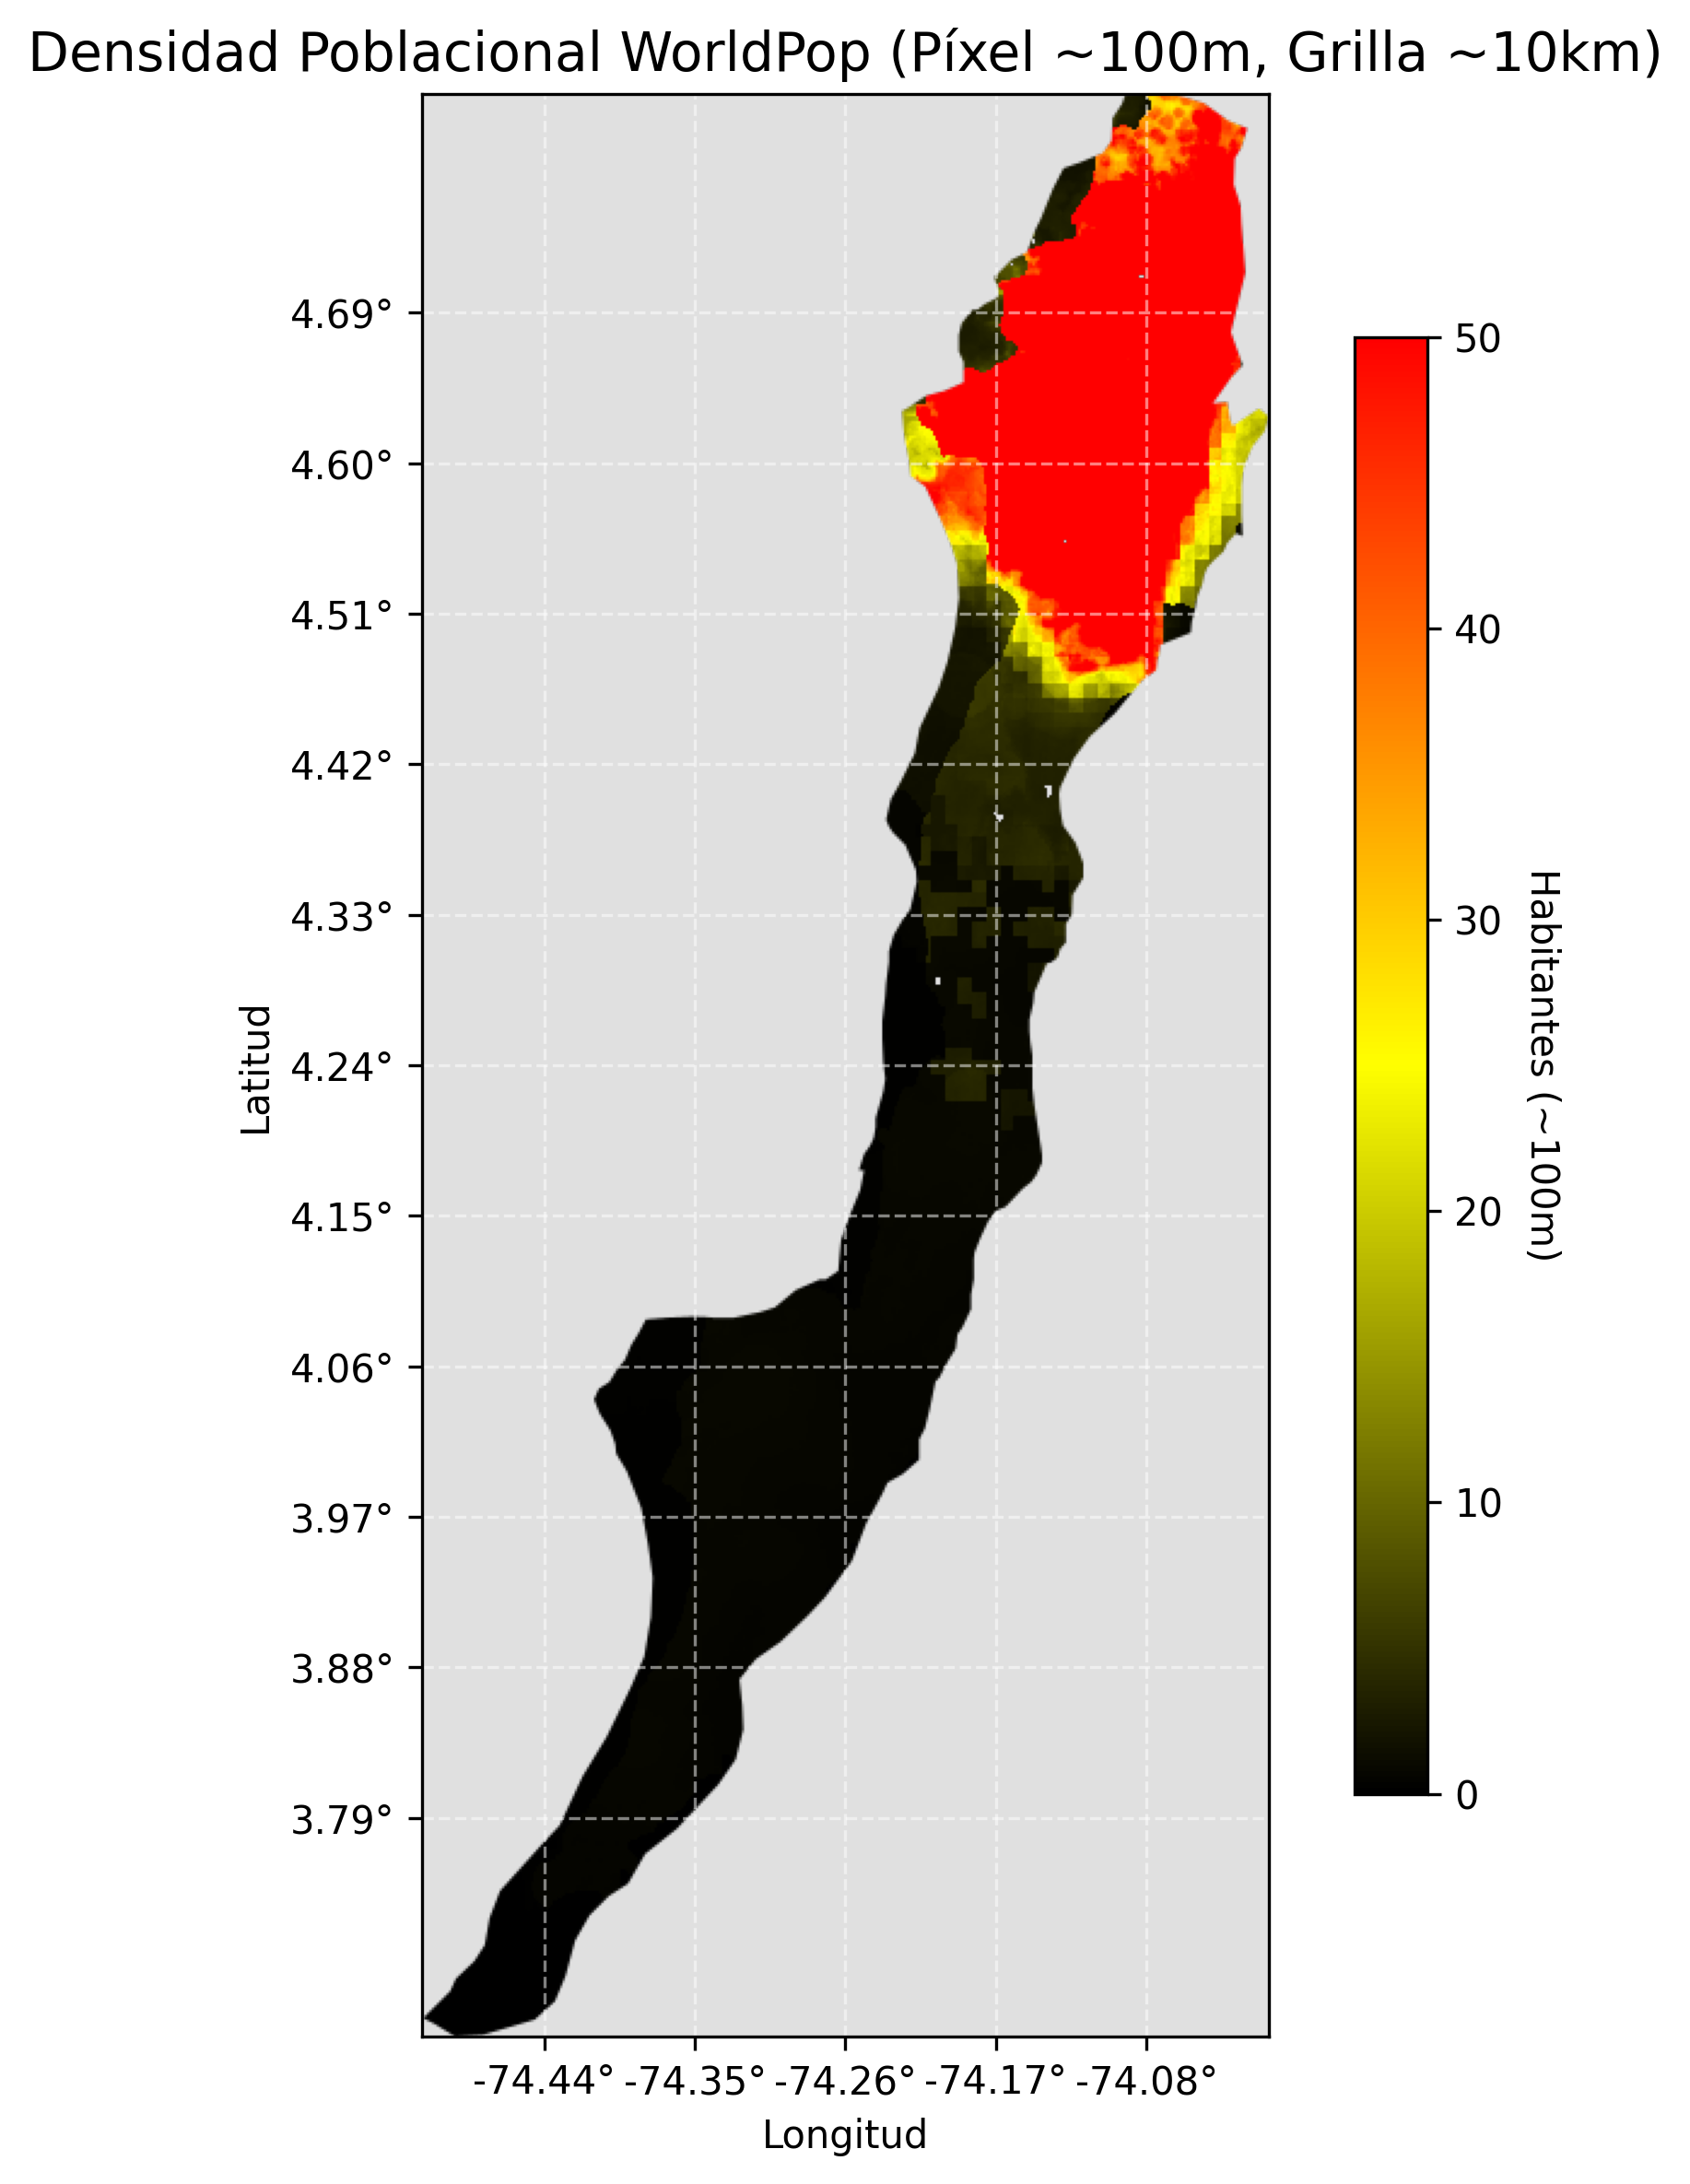
\includegraphics{45-practica_5_clase6_introduccion_sr_gee_files/figure-pdf/fig-python_pop_estatico-output-1.png}

}

\caption{\label{fig-python_pop_estatico}Mapa estático de densidad
poblacional (WorldPop) para la ciudad de Bogotá D.C., mostrando el
contraste entre la periferia y el centro urbano denso.}

\end{figure}%

\subsection{Javascript}

Para ejecutar este código, debes abrir el
\textbf{\href{https://code.earthengine.google.com/}{Code Editor de
Google Earth Engine}} en tu navegador, pegar el siguiente fragmento en
la consola central y hacer clic en \textbf{``Run''}.

\phantomsection\label{js_pop}%
\begin{Shaded}
\begin{Highlighting}[]
\CommentTok{// 1. DEFINICIÓN DEL PUNTO GEOGRÁFICO}
\KeywordTok{var}\NormalTok{ punto\_unal }\OperatorTok{=}\NormalTok{ ee}\OperatorTok{.}\AttributeTok{Geometry}\OperatorTok{.}\FunctionTok{Point}\NormalTok{([}\OperatorTok{{-}}\FloatTok{74.084}\OperatorTok{,} \FloatTok{4.638}\NormalTok{])}\OperatorTok{;}

\CommentTok{// 2. CENTRAR EL VISOR}
\BuiltInTok{Map}\OperatorTok{.}\FunctionTok{centerObject}\NormalTok{(punto\_unal}\OperatorTok{,} \DecValTok{17}\NormalTok{)}\OperatorTok{;}

\CommentTok{// 3. CONSULTA Y FILTRADO DE DATOS}
\KeywordTok{var}\NormalTok{ pop }\OperatorTok{=}\NormalTok{ ee}\OperatorTok{.}\FunctionTok{ImageCollection}\NormalTok{(}\StringTok{"WorldPop/GP/100m/pop"}\NormalTok{)}\OperatorTok{.}\FunctionTok{filter}\NormalTok{(ee}\OperatorTok{.}\AttributeTok{Filter}\OperatorTok{.}\FunctionTok{eq}\NormalTok{(}\StringTok{\textquotesingle{}country\textquotesingle{}}\OperatorTok{,} \StringTok{\textquotesingle{}COL\textquotesingle{}}\NormalTok{))}\OperatorTok{.}\FunctionTok{first}\NormalTok{()}\OperatorTok{;}

\CommentTok{// 4. PARÁMETROS DE VISUALIZACIÓN}
\KeywordTok{var}\NormalTok{ visParams }\OperatorTok{=}\NormalTok{ \{}\DataTypeTok{min}\OperatorTok{:} \DecValTok{0}\OperatorTok{,} \DataTypeTok{max}\OperatorTok{:} \DecValTok{50}\OperatorTok{,} \DataTypeTok{palette}\OperatorTok{:}\NormalTok{ [}\StringTok{\textquotesingle{}black\textquotesingle{}}\OperatorTok{,} \StringTok{\textquotesingle{}yellow\textquotesingle{}}\OperatorTok{,} \StringTok{\textquotesingle{}red\textquotesingle{}}\NormalTok{]\}}\OperatorTok{;}

\CommentTok{// 5. MOSTRAR EN PANTALLA Y EN CONSOLA}
\BuiltInTok{Map}\OperatorTok{.}\FunctionTok{addLayer}\NormalTok{(pop}\OperatorTok{,}\NormalTok{ visParams}\OperatorTok{,} \StringTok{\textquotesingle{}Densidad Poblacional {-} Colombia\textquotesingle{}}\NormalTok{)}\OperatorTok{;}

\FunctionTok{print}\NormalTok{(}\StringTok{\textquotesingle{}Metadatos de la imagen WorldPop:\textquotesingle{}}\OperatorTok{,}\NormalTok{ pop)}\OperatorTok{;}
\FunctionTok{print}\NormalTok{(}\StringTok{\textquotesingle{}ID exacto de la imagen WorldPop:\textquotesingle{}}\OperatorTok{,}\NormalTok{ pop}\OperatorTok{.}\FunctionTok{get}\NormalTok{(}\StringTok{\textquotesingle{}system:id\textquotesingle{}}\NormalTok{))}\OperatorTok{;}
\end{Highlighting}
\end{Shaded}

\begin{center}\rule{0.5\linewidth}{0.5pt}\end{center}

\phantomsection\label{js_pop_estatico}%
\begin{Shaded}
\begin{Highlighting}[]
\CommentTok{// ▷ CÓDIGO MAPA ESTÁTICO (THUMBNAIL) EN JAVASCRIPT (Independiente)}

\CommentTok{// 1. DEFINICIÓN DEL ÁREA (BOGOTÁ COMPLETA)}
\KeywordTok{var}\NormalTok{ localidades }\OperatorTok{=}\NormalTok{ ee}\OperatorTok{.}\FunctionTok{FeatureCollection}\NormalTok{(}\StringTok{"FAO/GAUL/2015/level2"}\NormalTok{)}\OperatorTok{;}
\KeywordTok{var}\NormalTok{ bogota }\OperatorTok{=}\NormalTok{ localidades}\OperatorTok{.}\FunctionTok{filter}\NormalTok{(ee}\OperatorTok{.}\AttributeTok{Filter}\OperatorTok{.}\FunctionTok{eq}\NormalTok{(}\StringTok{\textquotesingle{}ADM2\_NAME\textquotesingle{}}\OperatorTok{,} \StringTok{\textquotesingle{}Santafe De Bogota D.c.\textquotesingle{}}\NormalTok{))}\OperatorTok{;}
\KeywordTok{var}\NormalTok{ region\_interes }\OperatorTok{=}\NormalTok{ bogota}\OperatorTok{.}\FunctionTok{geometry}\NormalTok{()}\OperatorTok{.}\FunctionTok{bounds}\NormalTok{()}\OperatorTok{;}

\CommentTok{// 2. CONSULTA Y PROCESAMIENTO DE LA IMAGEN}
\KeywordTok{var}\NormalTok{ pop\_estatica }\OperatorTok{=}\NormalTok{ ee}\OperatorTok{.}\FunctionTok{ImageCollection}\NormalTok{(}\StringTok{"WorldPop/GP/100m/pop"}\NormalTok{)}
  \OperatorTok{.}\FunctionTok{filter}\NormalTok{(ee}\OperatorTok{.}\AttributeTok{Filter}\OperatorTok{.}\FunctionTok{eq}\NormalTok{(}\StringTok{\textquotesingle{}country\textquotesingle{}}\OperatorTok{,} \StringTok{\textquotesingle{}COL\textquotesingle{}}\NormalTok{))}
  \OperatorTok{.}\FunctionTok{first}\NormalTok{()}
  \OperatorTok{.}\FunctionTok{clip}\NormalTok{(bogota)}\OperatorTok{;}

\CommentTok{// 3. PARÁMETROS DE VISUALIZACIÓN}
\KeywordTok{var}\NormalTok{ visParamsEstatica }\OperatorTok{=}\NormalTok{ \{}
  \DataTypeTok{min}\OperatorTok{:} \DecValTok{0}\OperatorTok{,}
  \DataTypeTok{max}\OperatorTok{:} \DecValTok{50}\OperatorTok{,}
  \DataTypeTok{palette}\OperatorTok{:}\NormalTok{ [}\StringTok{\textquotesingle{}black\textquotesingle{}}\OperatorTok{,} \StringTok{\textquotesingle{}yellow\textquotesingle{}}\OperatorTok{,} \StringTok{\textquotesingle{}red\textquotesingle{}}\NormalTok{]}\OperatorTok{,}
  \DataTypeTok{dimensions}\OperatorTok{:} \DecValTok{800}\OperatorTok{,}
  \DataTypeTok{region}\OperatorTok{:}\NormalTok{ region\_interes}
\NormalTok{\}}\OperatorTok{;}

\CommentTok{// 4. MOSTRAR EN CONSOLA LA URL Y EL THUMBNAIL}
\FunctionTok{print}\NormalTok{(}\StringTok{\textquotesingle{}URL PNG (Bogotá Completa 0{-}50):\textquotesingle{}}\OperatorTok{,}\NormalTok{ pop\_estatica}\OperatorTok{.}\FunctionTok{getThumbURL}\NormalTok{(visParamsEstatica))}\OperatorTok{;}

\KeywordTok{var}\NormalTok{ miniatura }\OperatorTok{=}\NormalTok{ ui}\OperatorTok{.}\FunctionTok{Thumbnail}\NormalTok{(\{}
  \DataTypeTok{image}\OperatorTok{:}\NormalTok{ pop\_estatica}\OperatorTok{,}
  \DataTypeTok{params}\OperatorTok{:}\NormalTok{ visParamsEstatica}\OperatorTok{,}
  \DataTypeTok{style}\OperatorTok{:}\NormalTok{ \{}\DataTypeTok{width}\OperatorTok{:} \StringTok{\textquotesingle{}400px\textquotesingle{}}\OperatorTok{,} \DataTypeTok{height}\OperatorTok{:} \StringTok{\textquotesingle{}400px\textquotesingle{}}\OperatorTok{,} \DataTypeTok{backgroundColor}\OperatorTok{:} \StringTok{\textquotesingle{}\#e0e0e0\textquotesingle{}}\NormalTok{\}}
\NormalTok{\})}\OperatorTok{;}
\FunctionTok{print}\NormalTok{(}\StringTok{\textquotesingle{}Vista previa estática (Densidad Bogotá):\textquotesingle{}}\OperatorTok{,}\NormalTok{ miniatura)}\OperatorTok{;}
\end{Highlighting}
\end{Shaded}

\begin{center}\rule{0.5\linewidth}{0.5pt}\end{center}

\subsection{Reto: Carga de densidad poblacional en QGIS y ArcGIS
Pro}\label{reto-carga-de-densidad-poblacional-en-qgis-y-arcgis-pro}

Proceda a importar la capa de densidad poblacional en su entorno SIG de
escritorio.

\textbf{Instrucciones:}

\begin{enumerate}
\def\labelenumi{\arabic{enumi}.}
\tightlist
\item
  Ejecute el código de Python correspondiente para generar el archivo
  \texttt{pop\_serializado.json}.
\item
  En \textbf{QGIS}, emplee la pestaña \emph{Load} del plugin de GEE para
  cargar el Asset ID. Defina la paleta de colores y el rango (\texttt{0}
  a \texttt{50}).
\item
  En \textbf{ArcGIS Pro}, utilice la herramienta \emph{Add Image to Map
  by Serialized Object} o su equivalente mediante Asset ID.
\item
  \textbf{Reporte:} Capture la pantalla de las herramientas configuradas
  antes de su ejecución e insértelas a continuación.
\end{enumerate}

\begin{quote}
\textbf{Reporte visual de WorldPop}

\emph{Captura de QGIS (Pestaña Load):}
\texttt{!{[}Parámetros\ de\ WorldPop\ en\ QGIS{]}(ruta/a/tu/captura\_qgis\_pop.png)\{fig-align="center"\ width="80\%"\}}

\emph{Captura de ArcGIS Pro (Herramienta utilizada):}
\texttt{!{[}Parámetros\ de\ WorldPop\ en\ ArcGIS\ Pro{]}(ruta/a/tu/captura\_arcgis\_pop.png)\{fig-align="center"\ width="80\%"\}}
\end{quote}

\section{Filtrado de datos espaciales y recortes (querying y
clipping)}\label{filtrado-de-datos-espaciales-y-recortes-querying-y-clipping}

El procesamiento de imágenes satelitales a menudo requiere restringir
los datos a un área de estudio específica para optimizar los tiempos de
cómputo y la memoria.

\begin{longtable}[]{@{}
  >{\raggedright\arraybackslash}p{(\columnwidth - 4\tabcolsep) * \real{0.3333}}
  >{\raggedright\arraybackslash}p{(\columnwidth - 4\tabcolsep) * \real{0.3333}}
  >{\raggedright\arraybackslash}p{(\columnwidth - 4\tabcolsep) * \real{0.3333}}@{}}
\toprule\noalign{}
\begin{minipage}[b]{\linewidth}\raggedright
Filtro
\end{minipage} & \begin{minipage}[b]{\linewidth}\raggedright
Descripción
\end{minipage} & \begin{minipage}[b]{\linewidth}\raggedright
Ejemplo
\end{minipage} \\
\midrule\noalign{}
\endhead
\bottomrule\noalign{}
\endlastfoot
\texttt{filterBounds} & Filtra espacialmente por geometría &
\texttt{.filterBounds(geometria)} \\
\texttt{filterDate} & Filtra por rango de fechas &
\texttt{.filterDate(\textquotesingle{}2023-01-01\textquotesingle{},\ \textquotesingle{}2023-12-31\textquotesingle{})} \\
\texttt{filterMetadata} & Filtra por propiedades específicas &
\texttt{.filterMetadata(\textquotesingle{}CLOUDY\_PIXEL\_PERCENTAGE\textquotesingle{},\ \textquotesingle{}less\_than\textquotesingle{},\ 10)} \\
\end{longtable}

\subsection{Python}

\begin{Shaded}
\begin{Highlighting}[]
\CommentTok{\# \#| eval: false}

\CommentTok{\# Código usando Folium!}

\ImportTok{import}\NormalTok{ ee}
\ImportTok{import}\NormalTok{ folium}
\ImportTok{import}\NormalTok{ datetime}
\ImportTok{import}\NormalTok{ json}

\CommentTok{\# 1. DEFINICIÓN DEL PUNTO GEOGRÁFICO}
\NormalTok{unal\_punto }\OperatorTok{=}\NormalTok{ ee.Geometry.Point([}\OperatorTok{{-}}\FloatTok{74.084}\NormalTok{, }\FloatTok{4.638}\NormalTok{])}

\CommentTok{\# 2. CARGA DE VECTORES Y FILTRADO}
\NormalTok{localidades }\OperatorTok{=}\NormalTok{ ee.FeatureCollection(}\StringTok{"FAO/GAUL/2015/level2"}\NormalTok{)}
\NormalTok{bogota }\OperatorTok{=}\NormalTok{ localidades.}\BuiltInTok{filter}\NormalTok{(ee.Filter.eq(}\StringTok{\textquotesingle{}ADM2\_NAME\textquotesingle{}}\NormalTok{, }\StringTok{\textquotesingle{}Santafe De Bogota D.c.\textquotesingle{}}\NormalTok{))}

\CommentTok{\# 3. CARGA DE IMÁGENES Y RECORTE (CLIP)}
\NormalTok{coleccion\_s2 }\OperatorTok{=}\NormalTok{ (ee.ImageCollection(}\StringTok{"COPERNICUS/S2\_SR\_HARMONIZED"}\NormalTok{)}
\NormalTok{    .filterBounds(bogota)}
\NormalTok{    .filterDate(}\StringTok{\textquotesingle{}2023{-}01{-}01\textquotesingle{}}\NormalTok{, }\StringTok{\textquotesingle{}2023{-}06{-}30\textquotesingle{}}\NormalTok{)}
\NormalTok{    .}\BuiltInTok{filter}\NormalTok{(ee.Filter.lt(}\StringTok{\textquotesingle{}CLOUDY\_PIXEL\_PERCENTAGE\textquotesingle{}}\NormalTok{, }\DecValTok{10}\NormalTok{)))}

\NormalTok{s2\_base }\OperatorTok{=}\NormalTok{ ee.Image(coleccion\_s2.first())}
\NormalTok{s2\_clip }\OperatorTok{=}\NormalTok{ s2\_base.clip(bogota)}

\CommentTok{\# 4. EXPORTAR LOS ARCHIVOS JSON (METADATOS Y SERIALIZADO)}
\NormalTok{id\_exacto }\OperatorTok{=}\NormalTok{ s2\_base.get(}\StringTok{\textquotesingle{}system:id\textquotesingle{}}\NormalTok{).getInfo()}
\BuiltInTok{print}\NormalTok{(}\SpecialStringTok{f"}\CharTok{\textbackslash{}n}\SpecialStringTok{ID de la imagen Sentinel 2 base: }\SpecialCharTok{\{}\NormalTok{id\_exacto}\SpecialCharTok{\}}\SpecialStringTok{"}\NormalTok{)}

\NormalTok{metadatos\_json }\OperatorTok{=}\NormalTok{ s2\_base.getInfo()}
\ControlFlowTok{with} \BuiltInTok{open}\NormalTok{(}\StringTok{\textquotesingle{}metadatos\_s2\_clip.json\textquotesingle{}}\NormalTok{, }\StringTok{\textquotesingle{}w\textquotesingle{}}\NormalTok{) }\ImportTok{as}\NormalTok{ archivo:}
\NormalTok{    json.dump(metadatos\_json, archivo, indent}\OperatorTok{=}\DecValTok{4}\NormalTok{)}

\NormalTok{texto\_json\_serializado }\OperatorTok{=}\NormalTok{ s2\_clip.serialize()}
\ControlFlowTok{with} \BuiltInTok{open}\NormalTok{(}\StringTok{\textquotesingle{}s2\_clip\_serializado.json\textquotesingle{}}\NormalTok{, }\StringTok{\textquotesingle{}w\textquotesingle{}}\NormalTok{) }\ImportTok{as}\NormalTok{ archivo:}
\NormalTok{    json.dump(texto\_json\_serializado, archivo)}

\CommentTok{\# 5. PARÁMETROS DE VISUALIZACIÓN}
\NormalTok{vis\_params }\OperatorTok{=}\NormalTok{ \{}\StringTok{\textquotesingle{}bands\textquotesingle{}}\NormalTok{: [}\StringTok{\textquotesingle{}B4\textquotesingle{}}\NormalTok{, }\StringTok{\textquotesingle{}B3\textquotesingle{}}\NormalTok{, }\StringTok{\textquotesingle{}B2\textquotesingle{}}\NormalTok{], }\StringTok{\textquotesingle{}min\textquotesingle{}}\NormalTok{: }\DecValTok{0}\NormalTok{, }\StringTok{\textquotesingle{}max\textquotesingle{}}\NormalTok{: }\DecValTok{3000}\NormalTok{\}}
\NormalTok{map\_id\_img }\OperatorTok{=}\NormalTok{ ee.Image(s2\_clip).getMapId(vis\_params)}

\CommentTok{\# Visualización del borde del polígono}
\NormalTok{borde\_bogota }\OperatorTok{=}\NormalTok{ ee.Image().paint(bogota, }\DecValTok{0}\NormalTok{, }\DecValTok{2}\NormalTok{)}
\NormalTok{map\_id\_vector }\OperatorTok{=}\NormalTok{ borde\_bogota.getMapId(\{}\StringTok{\textquotesingle{}palette\textquotesingle{}}\NormalTok{: [}\StringTok{\textquotesingle{}red\textquotesingle{}}\NormalTok{]\})}

\CommentTok{\# 6. CONFIGURACIÓN DEL MAPA BASE (Folium)}
\NormalTok{Map\_filtro }\OperatorTok{=}\NormalTok{ folium.Map(location}\OperatorTok{=}\NormalTok{[}\FloatTok{4.638}\NormalTok{, }\OperatorTok{{-}}\FloatTok{74.084}\NormalTok{], zoom\_start}\OperatorTok{=}\DecValTok{17}\NormalTok{)}

\CommentTok{\# 7. AGREGAR LAS CAPAS AL VISOR}
\NormalTok{folium.TileLayer(}
\NormalTok{    tiles}\OperatorTok{=}\NormalTok{map\_id\_img[}\StringTok{\textquotesingle{}tile\_fetcher\textquotesingle{}}\NormalTok{].url\_format,}
\NormalTok{    attr}\OperatorTok{=}\StringTok{\textquotesingle{}Google Earth Engine\textquotesingle{}}\NormalTok{,}
\NormalTok{    overlay}\OperatorTok{=}\VariableTok{True}\NormalTok{,}
\NormalTok{    name}\OperatorTok{=}\StringTok{\textquotesingle{}Bogotá Recortada (S2)\textquotesingle{}}
\NormalTok{).add\_to(Map\_filtro)}

\NormalTok{folium.TileLayer(}
\NormalTok{    tiles}\OperatorTok{=}\NormalTok{map\_id\_vector[}\StringTok{\textquotesingle{}tile\_fetcher\textquotesingle{}}\NormalTok{].url\_format,}
\NormalTok{    attr}\OperatorTok{=}\StringTok{\textquotesingle{}Google Earth Engine\textquotesingle{}}\NormalTok{,}
\NormalTok{    overlay}\OperatorTok{=}\VariableTok{True}\NormalTok{,}
\NormalTok{    name}\OperatorTok{=}\StringTok{\textquotesingle{}Límite Bogotá\textquotesingle{}}
\NormalTok{).add\_to(Map\_filtro)}

\NormalTok{folium.LayerControl().add\_to(Map\_filtro)}

\CommentTok{\# 8. VISUALIZACIÓN DEL RESULTADO}
\CommentTok{\# Map\_filtro}
\CommentTok{\# from IPython.display import display, HTML}
\CommentTok{\# display(HTML(Map\_filtro.\_repr\_html\_()))}

\ImportTok{from}\NormalTok{ IPython.display }\ImportTok{import}\NormalTok{ IFrame}

\CommentTok{\# Guardamos el mapa aislado en tu carpeta de trabajo}
\NormalTok{Map\_filtro.save(}\StringTok{"mapas/map\_filtro.html"}\NormalTok{)}

\CommentTok{\# Lo incrustamos en el documento Quarto como una página web independiente}
\NormalTok{display(IFrame(src}\OperatorTok{=}\StringTok{"mapas/map\_filtro.html"}\NormalTok{, width}\OperatorTok{=}\StringTok{"100\%"}\NormalTok{, height}\OperatorTok{=}\StringTok{"500px"}\NormalTok{))}
\end{Highlighting}
\end{Shaded}

\begin{verbatim}

ID de la imagen Sentinel 2 base: COPERNICUS/S2_SR_HARMONIZED/20230128T152639_20230128T152835_T18NXL
\end{verbatim}

\phantomsection\label{python_filtros}
\begin{verbatim}
<IPython.lib.display.IFrame at 0x7ac2a2c78bc0>
\end{verbatim}

\begin{center}\rule{0.5\linewidth}{0.5pt}\end{center}

\begin{Shaded}
\begin{Highlighting}[]
\CommentTok{\# \#| eval: false}

\CommentTok{\# ▷ CÓDIGO MAPA ESTÁTICO (PNG) PARA FOLIUM/GENERAL (Independiente)}
\ImportTok{import}\NormalTok{ ee}
\ImportTok{import}\NormalTok{ requests}
\ImportTok{import}\NormalTok{ matplotlib.pyplot }\ImportTok{as}\NormalTok{ plt}
\ImportTok{from}\NormalTok{ PIL }\ImportTok{import}\NormalTok{ Image}
\ImportTok{from}\NormalTok{ io }\ImportTok{import}\NormalTok{ BytesIO}

\CommentTok{\# 1. CARGA DE VECTORES Y DEFINICIÓN DEL ÁREA (BOGOTÁ COMPLETA)}
\NormalTok{localidades }\OperatorTok{=}\NormalTok{ ee.FeatureCollection(}\StringTok{"FAO/GAUL/2015/level2"}\NormalTok{)}
\NormalTok{bogota }\OperatorTok{=}\NormalTok{ localidades.}\BuiltInTok{filter}\NormalTok{(ee.Filter.eq(}\StringTok{\textquotesingle{}ADM2\_NAME\textquotesingle{}}\NormalTok{, }\StringTok{\textquotesingle{}Santafe De Bogota D.c.\textquotesingle{}}\NormalTok{))}
\NormalTok{region\_interes }\OperatorTok{=}\NormalTok{ bogota.geometry().bounds()}

\CommentTok{\# 2. CONSULTA, FILTRADO Y RECORTE DE LA IMAGEN}
\NormalTok{coleccion\_s2 }\OperatorTok{=}\NormalTok{ (ee.ImageCollection(}\StringTok{"COPERNICUS/S2\_SR\_HARMONIZED"}\NormalTok{)}
\NormalTok{    .filterBounds(bogota)}
\NormalTok{    .filterDate(}\StringTok{\textquotesingle{}2023{-}01{-}01\textquotesingle{}}\NormalTok{, }\StringTok{\textquotesingle{}2023{-}06{-}30\textquotesingle{}}\NormalTok{)}
\NormalTok{    .}\BuiltInTok{filter}\NormalTok{(ee.Filter.lt(}\StringTok{\textquotesingle{}CLOUDY\_PIXEL\_PERCENTAGE\textquotesingle{}}\NormalTok{, }\DecValTok{10}\NormalTok{)))}

\NormalTok{s2\_clip }\OperatorTok{=}\NormalTok{ ee.Image(coleccion\_s2.first()).clip(bogota)}

\CommentTok{\# 3. COMPOSICIÓN VISUAL (Fusionamos la imagen RGB con el borde vectorial)}
\NormalTok{s2\_rgb }\OperatorTok{=}\NormalTok{ s2\_clip.visualize(}\OperatorTok{**}\NormalTok{\{}\StringTok{\textquotesingle{}bands\textquotesingle{}}\NormalTok{: [}\StringTok{\textquotesingle{}B4\textquotesingle{}}\NormalTok{, }\StringTok{\textquotesingle{}B3\textquotesingle{}}\NormalTok{, }\StringTok{\textquotesingle{}B2\textquotesingle{}}\NormalTok{], }\StringTok{\textquotesingle{}min\textquotesingle{}}\NormalTok{: }\DecValTok{0}\NormalTok{, }\StringTok{\textquotesingle{}max\textquotesingle{}}\NormalTok{: }\DecValTok{3000}\NormalTok{\})}
\NormalTok{borde\_rojo }\OperatorTok{=}\NormalTok{ ee.Image().paint(bogota, }\DecValTok{0}\NormalTok{, }\DecValTok{2}\NormalTok{).visualize(}\OperatorTok{**}\NormalTok{\{}\StringTok{\textquotesingle{}palette\textquotesingle{}}\NormalTok{: [}\StringTok{\textquotesingle{}red\textquotesingle{}}\NormalTok{]\})}
\NormalTok{img\_final }\OperatorTok{=}\NormalTok{ s2\_rgb.blend(borde\_rojo)}

\CommentTok{\# 4. OBTENER LA URL DEL THUMBNAIL (PNG) DESDE GOOGLE EARTH ENGINE}
\NormalTok{url\_img }\OperatorTok{=}\NormalTok{ img\_final.getThumbURL(\{}
    \StringTok{\textquotesingle{}dimensions\textquotesingle{}}\NormalTok{: }\DecValTok{800}\NormalTok{,}
    \StringTok{\textquotesingle{}region\textquotesingle{}}\NormalTok{: region\_interes}
\NormalTok{\})}

\CommentTok{\# 5. DESCARGAR Y DIBUJAR LA IMAGEN CON MATPLOTLIB}
\NormalTok{respuesta }\OperatorTok{=}\NormalTok{ requests.get(url\_img)}
\NormalTok{imagen\_png }\OperatorTok{=}\NormalTok{ Image.}\BuiltInTok{open}\NormalTok{(BytesIO(respuesta.content))}

\NormalTok{coords }\OperatorTok{=}\NormalTok{ region\_interes.coordinates().get(}\DecValTok{0}\NormalTok{).getInfo()}
\NormalTok{xmin }\OperatorTok{=} \BuiltInTok{min}\NormalTok{([c[}\DecValTok{0}\NormalTok{] }\ControlFlowTok{for}\NormalTok{ c }\KeywordTok{in}\NormalTok{ coords])}
\NormalTok{xmax }\OperatorTok{=} \BuiltInTok{max}\NormalTok{([c[}\DecValTok{0}\NormalTok{] }\ControlFlowTok{for}\NormalTok{ c }\KeywordTok{in}\NormalTok{ coords])}
\NormalTok{ymin }\OperatorTok{=} \BuiltInTok{min}\NormalTok{([c[}\DecValTok{1}\NormalTok{] }\ControlFlowTok{for}\NormalTok{ c }\KeywordTok{in}\NormalTok{ coords])}
\NormalTok{ymax }\OperatorTok{=} \BuiltInTok{max}\NormalTok{([c[}\DecValTok{1}\NormalTok{] }\ControlFlowTok{for}\NormalTok{ c }\KeywordTok{in}\NormalTok{ coords])}

\NormalTok{fig, ax }\OperatorTok{=}\NormalTok{ plt.subplots(figsize}\OperatorTok{=}\NormalTok{(}\DecValTok{8}\NormalTok{, }\DecValTok{8}\NormalTok{))}

\NormalTok{ax.imshow(imagen\_png, extent}\OperatorTok{=}\NormalTok{[xmin, xmax, ymin, ymax])}

\CommentTok{\# Grilla de 10 km (1 grado ≈ 111 km {-}\textgreater{} 10 km ≈ 0.09 grados)}
\NormalTok{paso\_10km }\OperatorTok{=} \FloatTok{0.09} 
\NormalTok{lon\_centro, lat\_centro }\OperatorTok{=}\NormalTok{ (xmin }\OperatorTok{+}\NormalTok{ xmax) }\OperatorTok{/} \DecValTok{2}\NormalTok{, (ymin }\OperatorTok{+}\NormalTok{ ymax) }\OperatorTok{/} \DecValTok{2}
\NormalTok{x\_ticks }\OperatorTok{=}\NormalTok{ [lon\_centro }\OperatorTok{+}\NormalTok{ (i }\OperatorTok{*}\NormalTok{ paso\_10km) }\ControlFlowTok{for}\NormalTok{ i }\KeywordTok{in} \BuiltInTok{range}\NormalTok{(}\OperatorTok{{-}}\DecValTok{5}\NormalTok{, }\DecValTok{6}\NormalTok{)]}
\NormalTok{y\_ticks }\OperatorTok{=}\NormalTok{ [lat\_centro }\OperatorTok{+}\NormalTok{ (i }\OperatorTok{*}\NormalTok{ paso\_10km) }\ControlFlowTok{for}\NormalTok{ i }\KeywordTok{in} \BuiltInTok{range}\NormalTok{(}\OperatorTok{{-}}\DecValTok{5}\NormalTok{, }\DecValTok{6}\NormalTok{)]}

\NormalTok{x\_ticks }\OperatorTok{=}\NormalTok{ [x }\ControlFlowTok{for}\NormalTok{ x }\KeywordTok{in}\NormalTok{ x\_ticks }\ControlFlowTok{if}\NormalTok{ xmin }\OperatorTok{\textless{}=}\NormalTok{ x }\OperatorTok{\textless{}=}\NormalTok{ xmax]}
\NormalTok{y\_ticks }\OperatorTok{=}\NormalTok{ [y }\ControlFlowTok{for}\NormalTok{ y }\KeywordTok{in}\NormalTok{ y\_ticks }\ControlFlowTok{if}\NormalTok{ ymin }\OperatorTok{\textless{}=}\NormalTok{ y }\OperatorTok{\textless{}=}\NormalTok{ ymax]}

\NormalTok{ax.set\_xticks(x\_ticks)}
\NormalTok{ax.set\_yticks(y\_ticks)}
\NormalTok{ax.set\_xticklabels([}\SpecialStringTok{f"}\SpecialCharTok{\{}\NormalTok{x}\SpecialCharTok{:.2f\}}\SpecialStringTok{°"} \ControlFlowTok{for}\NormalTok{ x }\KeywordTok{in}\NormalTok{ x\_ticks])}
\NormalTok{ax.set\_yticklabels([}\SpecialStringTok{f"}\SpecialCharTok{\{}\NormalTok{y}\SpecialCharTok{:.2f\}}\SpecialStringTok{°"} \ControlFlowTok{for}\NormalTok{ y }\KeywordTok{in}\NormalTok{ y\_ticks])}

\NormalTok{ax.grid(color}\OperatorTok{=}\StringTok{\textquotesingle{}white\textquotesingle{}}\NormalTok{, linestyle}\OperatorTok{=}\StringTok{\textquotesingle{}{-}{-}\textquotesingle{}}\NormalTok{, linewidth}\OperatorTok{=}\DecValTok{1}\NormalTok{, alpha}\OperatorTok{=}\FloatTok{0.7}\NormalTok{)}
\NormalTok{ax.set\_title(}\StringTok{\textquotesingle{}Sentinel{-}2 Recortada {-} Bogotá D.C. (Grilla \textasciitilde{}10 km)\textquotesingle{}}\NormalTok{, fontsize}\OperatorTok{=}\DecValTok{14}\NormalTok{)}
\NormalTok{ax.set\_xlabel(}\StringTok{\textquotesingle{}Longitud\textquotesingle{}}\NormalTok{)}
\NormalTok{ax.set\_ylabel(}\StringTok{\textquotesingle{}Latitud\textquotesingle{}}\NormalTok{)}

\NormalTok{ax.set\_facecolor(}\StringTok{\textquotesingle{}\#e0e0e0\textquotesingle{}}\NormalTok{) }

\NormalTok{plt.tight\_layout()}
\NormalTok{plt.show()}
\end{Highlighting}
\end{Shaded}

\begin{figure}[H]

\centering{

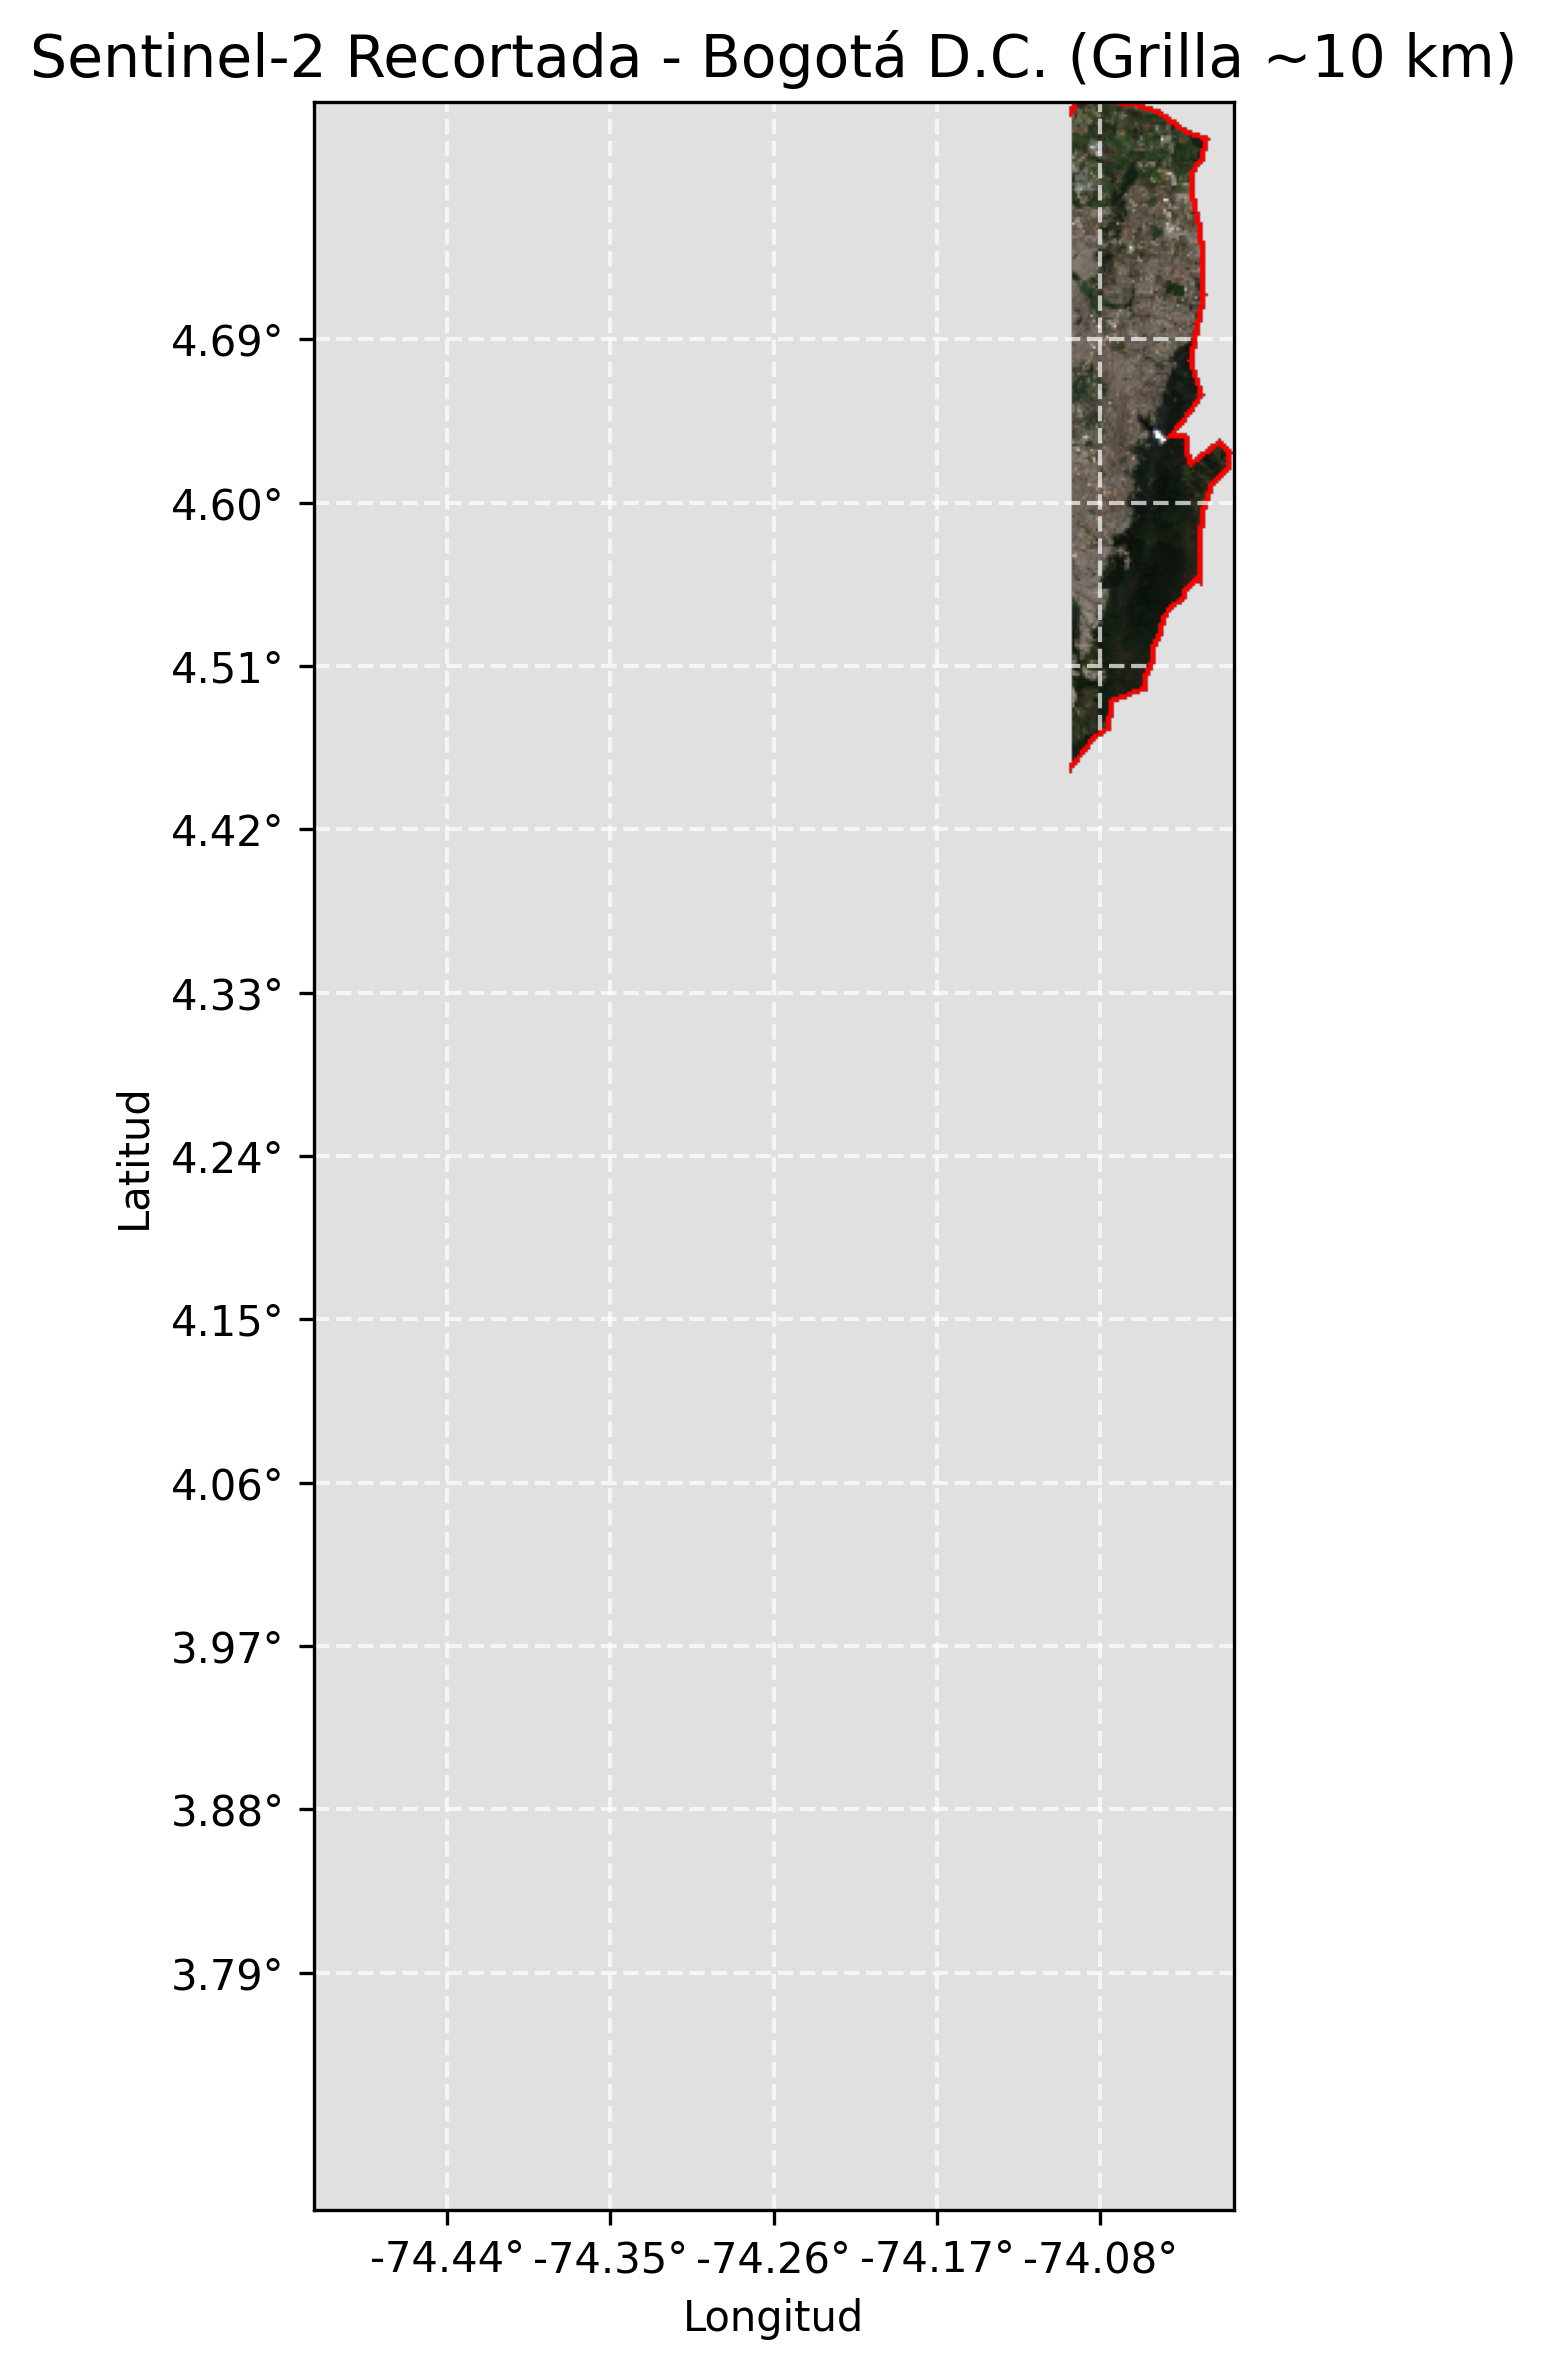
\includegraphics{45-practica_5_clase6_introduccion_sr_gee_files/figure-pdf/fig-python_filtros_estatico-output-1.png}

}

\caption{\label{fig-python_filtros_estatico}Mapa estático de la ciudad
de Bogotá D.C., recortado sobre una imagen Sentinel-2 con grilla
geográfica.}

\end{figure}%

\subsection{Javascript}

Para ejecutar este código, debes abrir el
\textbf{\href{https://code.earthengine.google.com/}{Code Editor de
Google Earth Engine}} en tu navegador, pegar el siguiente fragmento en
la consola central y hacer clic en \textbf{``Run''}.

\phantomsection\label{js_filtros}%
\begin{Shaded}
\begin{Highlighting}[]
\CommentTok{// 1. DEFINICIÓN DEL PUNTO GEOGRÁFICO}
\KeywordTok{var}\NormalTok{ punto\_unal }\OperatorTok{=}\NormalTok{ ee}\OperatorTok{.}\AttributeTok{Geometry}\OperatorTok{.}\FunctionTok{Point}\NormalTok{([}\OperatorTok{{-}}\FloatTok{74.084}\OperatorTok{,} \FloatTok{4.638}\NormalTok{])}\OperatorTok{;}

\CommentTok{// 2. CENTRAR EL VISOR}
\BuiltInTok{Map}\OperatorTok{.}\FunctionTok{centerObject}\NormalTok{(punto\_unal}\OperatorTok{,} \DecValTok{17}\NormalTok{)}\OperatorTok{;}

\CommentTok{// 3. CARGA DE VECTORES Y FILTRADO}
\KeywordTok{var}\NormalTok{ localidades }\OperatorTok{=}\NormalTok{ ee}\OperatorTok{.}\FunctionTok{FeatureCollection}\NormalTok{(}\StringTok{"FAO/GAUL/2015/level2"}\NormalTok{)}\OperatorTok{;}
\KeywordTok{var}\NormalTok{ bogota }\OperatorTok{=}\NormalTok{ localidades}\OperatorTok{.}\FunctionTok{filter}\NormalTok{(ee}\OperatorTok{.}\AttributeTok{Filter}\OperatorTok{.}\FunctionTok{eq}\NormalTok{(}\StringTok{\textquotesingle{}ADM2\_NAME\textquotesingle{}}\OperatorTok{,} \StringTok{\textquotesingle{}Santafe De Bogota D.c.\textquotesingle{}}\NormalTok{))}\OperatorTok{;}

\CommentTok{// 4. CONSULTA, FILTRADO Y RECORTE DE LA IMAGEN}
\KeywordTok{var}\NormalTok{ coleccion\_s2 }\OperatorTok{=}\NormalTok{ ee}\OperatorTok{.}\FunctionTok{ImageCollection}\NormalTok{(}\StringTok{"COPERNICUS/S2\_SR\_HARMONIZED"}\NormalTok{)}
  \OperatorTok{.}\FunctionTok{filterBounds}\NormalTok{(bogota)}
  \OperatorTok{.}\FunctionTok{filterDate}\NormalTok{(}\StringTok{\textquotesingle{}2023{-}01{-}01\textquotesingle{}}\OperatorTok{,} \StringTok{\textquotesingle{}2023{-}06{-}30\textquotesingle{}}\NormalTok{)}
  \OperatorTok{.}\FunctionTok{filter}\NormalTok{(ee}\OperatorTok{.}\AttributeTok{Filter}\OperatorTok{.}\FunctionTok{lt}\NormalTok{(}\StringTok{\textquotesingle{}CLOUDY\_PIXEL\_PERCENTAGE\textquotesingle{}}\OperatorTok{,} \DecValTok{10}\NormalTok{))}\OperatorTok{;}

\KeywordTok{var}\NormalTok{ s2\_base }\OperatorTok{=}\NormalTok{ ee}\OperatorTok{.}\FunctionTok{Image}\NormalTok{(coleccion\_s2}\OperatorTok{.}\FunctionTok{first}\NormalTok{())}\OperatorTok{;}
\KeywordTok{var}\NormalTok{ s2\_clip }\OperatorTok{=}\NormalTok{ s2\_base}\OperatorTok{.}\FunctionTok{clip}\NormalTok{(bogota)}\OperatorTok{;}

\CommentTok{// 5. PARÁMETROS DE VISUALIZACIÓN}
\KeywordTok{var}\NormalTok{ visParams }\OperatorTok{=}\NormalTok{ \{}\DataTypeTok{bands}\OperatorTok{:}\NormalTok{ [}\StringTok{\textquotesingle{}B4\textquotesingle{}}\OperatorTok{,} \StringTok{\textquotesingle{}B3\textquotesingle{}}\OperatorTok{,} \StringTok{\textquotesingle{}B2\textquotesingle{}}\NormalTok{]}\OperatorTok{,} \DataTypeTok{min}\OperatorTok{:} \DecValTok{0}\OperatorTok{,} \DataTypeTok{max}\OperatorTok{:} \DecValTok{3000}\NormalTok{\}}\OperatorTok{;}

\CommentTok{// 6. MOSTRAR EN PANTALLA Y EN CONSOLA}
\BuiltInTok{Map}\OperatorTok{.}\FunctionTok{addLayer}\NormalTok{(s2\_clip}\OperatorTok{,}\NormalTok{ visParams}\OperatorTok{,} \StringTok{\textquotesingle{}Bogotá Recortada (S2)\textquotesingle{}}\NormalTok{)}\OperatorTok{;}
\BuiltInTok{Map}\OperatorTok{.}\FunctionTok{addLayer}\NormalTok{(ee}\OperatorTok{.}\FunctionTok{Image}\NormalTok{()}\OperatorTok{.}\FunctionTok{paint}\NormalTok{(bogota}\OperatorTok{,} \DecValTok{0}\OperatorTok{,} \DecValTok{2}\NormalTok{)}\OperatorTok{,}\NormalTok{ \{}\DataTypeTok{palette}\OperatorTok{:}\NormalTok{ [}\StringTok{\textquotesingle{}red\textquotesingle{}}\NormalTok{]\}}\OperatorTok{,} \StringTok{\textquotesingle{}Límite Bogotá\textquotesingle{}}\NormalTok{)}\OperatorTok{;}

\FunctionTok{print}\NormalTok{(}\StringTok{\textquotesingle{}Metadatos de la imagen base:\textquotesingle{}}\OperatorTok{,}\NormalTok{ s2\_base)}\OperatorTok{;}
\FunctionTok{print}\NormalTok{(}\StringTok{\textquotesingle{}ID exacto de la imagen base:\textquotesingle{}}\OperatorTok{,}\NormalTok{ s2\_base}\OperatorTok{.}\FunctionTok{get}\NormalTok{(}\StringTok{\textquotesingle{}system:id\textquotesingle{}}\NormalTok{))}\OperatorTok{;}
\end{Highlighting}
\end{Shaded}

\begin{center}\rule{0.5\linewidth}{0.5pt}\end{center}

\phantomsection\label{js_filtros_estatico}%
\begin{Shaded}
\begin{Highlighting}[]
\CommentTok{// ▷ CÓDIGO MAPA ESTÁTICO (THUMBNAIL) EN JAVASCRIPT (Independiente)}

\CommentTok{// 1. CARGA DE VECTORES Y DEFINICIÓN DEL ÁREA (BOGOTÁ COMPLETA)}
\KeywordTok{var}\NormalTok{ localidades }\OperatorTok{=}\NormalTok{ ee}\OperatorTok{.}\FunctionTok{FeatureCollection}\NormalTok{(}\StringTok{"FAO/GAUL/2015/level2"}\NormalTok{)}\OperatorTok{;}
\KeywordTok{var}\NormalTok{ bogota }\OperatorTok{=}\NormalTok{ localidades}\OperatorTok{.}\FunctionTok{filter}\NormalTok{(ee}\OperatorTok{.}\AttributeTok{Filter}\OperatorTok{.}\FunctionTok{eq}\NormalTok{(}\StringTok{\textquotesingle{}ADM2\_NAME\textquotesingle{}}\OperatorTok{,} \StringTok{\textquotesingle{}Santafe De Bogota D.c.\textquotesingle{}}\NormalTok{))}\OperatorTok{;}
\KeywordTok{var}\NormalTok{ region\_interes }\OperatorTok{=}\NormalTok{ bogota}\OperatorTok{.}\FunctionTok{geometry}\NormalTok{()}\OperatorTok{.}\FunctionTok{bounds}\NormalTok{()}\OperatorTok{;}

\CommentTok{// 2. CONSULTA, FILTRADO Y RECORTE DE LA IMAGEN}
\KeywordTok{var}\NormalTok{ coleccion\_s2 }\OperatorTok{=}\NormalTok{ ee}\OperatorTok{.}\FunctionTok{ImageCollection}\NormalTok{(}\StringTok{"COPERNICUS/S2\_SR\_HARMONIZED"}\NormalTok{)}
  \OperatorTok{.}\FunctionTok{filterBounds}\NormalTok{(bogota)}
  \OperatorTok{.}\FunctionTok{filterDate}\NormalTok{(}\StringTok{\textquotesingle{}2023{-}01{-}01\textquotesingle{}}\OperatorTok{,} \StringTok{\textquotesingle{}2023{-}06{-}30\textquotesingle{}}\NormalTok{)}
  \OperatorTok{.}\FunctionTok{filter}\NormalTok{(ee}\OperatorTok{.}\AttributeTok{Filter}\OperatorTok{.}\FunctionTok{lt}\NormalTok{(}\StringTok{\textquotesingle{}CLOUDY\_PIXEL\_PERCENTAGE\textquotesingle{}}\OperatorTok{,} \DecValTok{10}\NormalTok{))}\OperatorTok{;}

\KeywordTok{var}\NormalTok{ s2\_clip }\OperatorTok{=}\NormalTok{ ee}\OperatorTok{.}\FunctionTok{Image}\NormalTok{(coleccion\_s2}\OperatorTok{.}\FunctionTok{first}\NormalTok{())}\OperatorTok{.}\FunctionTok{clip}\NormalTok{(bogota)}\OperatorTok{;}

\CommentTok{// 3. COMPOSICIÓN VISUAL (Fusionamos la imagen RGB con el borde vectorial)}
\KeywordTok{var}\NormalTok{ s2\_rgb }\OperatorTok{=}\NormalTok{ s2\_clip}\OperatorTok{.}\FunctionTok{visualize}\NormalTok{(\{}\DataTypeTok{bands}\OperatorTok{:}\NormalTok{ [}\StringTok{\textquotesingle{}B4\textquotesingle{}}\OperatorTok{,} \StringTok{\textquotesingle{}B3\textquotesingle{}}\OperatorTok{,} \StringTok{\textquotesingle{}B2\textquotesingle{}}\NormalTok{]}\OperatorTok{,} \DataTypeTok{min}\OperatorTok{:} \DecValTok{0}\OperatorTok{,} \DataTypeTok{max}\OperatorTok{:} \DecValTok{3000}\NormalTok{\})}\OperatorTok{;}
\KeywordTok{var}\NormalTok{ borde\_rojo }\OperatorTok{=}\NormalTok{ ee}\OperatorTok{.}\FunctionTok{Image}\NormalTok{()}\OperatorTok{.}\FunctionTok{paint}\NormalTok{(bogota}\OperatorTok{,} \DecValTok{0}\OperatorTok{,} \DecValTok{2}\NormalTok{)}\OperatorTok{.}\FunctionTok{visualize}\NormalTok{(\{}\DataTypeTok{palette}\OperatorTok{:}\NormalTok{ [}\StringTok{\textquotesingle{}red\textquotesingle{}}\NormalTok{]\})}\OperatorTok{;}
\KeywordTok{var}\NormalTok{ img\_final }\OperatorTok{=}\NormalTok{ s2\_rgb}\OperatorTok{.}\FunctionTok{blend}\NormalTok{(borde\_rojo)}\OperatorTok{;}

\CommentTok{// 4. PARÁMETROS DE VISUALIZACIÓN}
\KeywordTok{var}\NormalTok{ visParamsEstatica }\OperatorTok{=}\NormalTok{ \{}
  \DataTypeTok{dimensions}\OperatorTok{:} \DecValTok{800}\OperatorTok{,}
  \DataTypeTok{region}\OperatorTok{:}\NormalTok{ region\_interes}
\NormalTok{\}}\OperatorTok{;}

\CommentTok{// 5. MOSTRAR EN CONSOLA LA URL Y EL THUMBNAIL}
\FunctionTok{print}\NormalTok{(}\StringTok{\textquotesingle{}URL de la imagen PNG:\textquotesingle{}}\OperatorTok{,}\NormalTok{ img\_final}\OperatorTok{.}\FunctionTok{getThumbURL}\NormalTok{(visParamsEstatica))}\OperatorTok{;}

\KeywordTok{var}\NormalTok{ miniatura }\OperatorTok{=}\NormalTok{ ui}\OperatorTok{.}\FunctionTok{Thumbnail}\NormalTok{(\{}
  \DataTypeTok{image}\OperatorTok{:}\NormalTok{ img\_final}\OperatorTok{,}
  \DataTypeTok{params}\OperatorTok{:}\NormalTok{ visParamsEstatica}\OperatorTok{,}
  \DataTypeTok{style}\OperatorTok{:}\NormalTok{ \{}\DataTypeTok{width}\OperatorTok{:} \StringTok{\textquotesingle{}400px\textquotesingle{}}\OperatorTok{,} \DataTypeTok{height}\OperatorTok{:} \StringTok{\textquotesingle{}400px\textquotesingle{}}\OperatorTok{,} \DataTypeTok{backgroundColor}\OperatorTok{:} \StringTok{\textquotesingle{}\#e0e0e0\textquotesingle{}}\OperatorTok{,} \DataTypeTok{border}\OperatorTok{:} \StringTok{\textquotesingle{}1px solid black\textquotesingle{}}\NormalTok{\}}
\NormalTok{\})}\OperatorTok{;}
\FunctionTok{print}\NormalTok{(}\StringTok{\textquotesingle{}Vista previa estática (Bogotá Recortada):\textquotesingle{}}\OperatorTok{,}\NormalTok{ miniatura)}\OperatorTok{;}
\end{Highlighting}
\end{Shaded}

\begin{center}\rule{0.5\linewidth}{0.5pt}\end{center}

\subsection{Reto: Carga de imagen con geoproceso de recorte en QGIS y
ArcGIS
Pro}\label{reto-carga-de-imagen-con-geoproceso-de-recorte-en-qgis-y-arcgis-pro}

Proceda a importar la imagen recortada en su entorno SIG de escritorio.
Tenga en cuenta que el archivo JSON generado
(\texttt{s2\_clip\_serializado.json}) contiene en su interior tanto la
instrucción de carga de la imagen como el geoproceso de recorte
(\texttt{clip}) definido en código.

\textbf{Instrucciones:}

\begin{enumerate}
\def\labelenumi{\arabic{enumi}.}
\tightlist
\item
  Ejecute el código de Python correspondiente para generar el archivo
  \texttt{s2\_clip\_serializado.json}.
\item
  En \textbf{ArcGIS Pro}, utilice la herramienta \emph{Add Image to Map
  by Serialized Object}. Al utilizar el archivo JSON, la herramienta
  procesará el recorte en los servidores de Google y desplegará la
  imagen ya ajustada al límite de Bogotá.
\item
  En \textbf{QGIS}, la pestaña \emph{Load} del plugin no procesa
  operaciones complejas como recortes. Utilice la opción de cargar la
  imagen base mediante el Asset ID, o utilice la pestaña \emph{Code}
  para correr el script completo en Python.
\item
  \textbf{Reporte:} Capture la pantalla de las herramientas configuradas
  antes de su ejecución e insértelas a continuación.
\end{enumerate}

\begin{quote}
\textbf{Reporte visual de geoprocesos (clipping)}

\emph{Captura de QGIS (Pestaña Code o Load):}
\texttt{!{[}Parámetros\ de\ recorte\ en\ QGIS{]}(ruta/a/tu/captura\_qgis\_clip.png)\{fig-align="center"\ width="80\%"\}}

\emph{Captura de ArcGIS Pro (Herramienta utilizada):}
\texttt{!{[}Parámetros\ de\ recorte\ en\ ArcGIS\ Pro{]}(ruta/a/tu/captura\_arcgis\_clip.png)\{fig-align="center"\ width="80\%"\}}
\end{quote}

\section{Índices espectrales (NDVI)}\label{uxedndices-espectrales-ndvi}

El álgebra de mapas permite combinar diferentes bandas para resaltar
características específicas de la superficie. El Índice de Vegetación de
Diferencia Normalizada (NDVI) es el índice más utilizado para analizar
el vigor vegetal, aprovechando la alta reflectancia de las plantas sanas
en el infrarrojo cercano (NIR) y la absorción en el rojo (Red).

La lógica del NDVI se basa en que la vegetación densa absorbe la mayor
parte de la luz roja que le llega y refleja una gran parte de la luz
infrarroja cercana. El resultado es un rango numérico que oscila
estrictamente entre \textbf{-1.0 y 1.0}, con la siguiente interpretación
física:

\begin{itemize}
\tightlist
\item
  \textbf{Valores negativos (Cercanos a -1):} Generalmente corresponden
  a cuerpos de agua, nieve o nubes, que reflejan más luz roja que
  infrarroja.
\item
  \textbf{Valores cercanos a cero (-0.1 a 0.1):} Representan áreas
  estériles de roca, arena o suelo desnudo.
\item
  \textbf{Valores positivos bajos (0.2 a 0.4):} Indican presencia de
  arbustos, pastizales o vegetación dispersa y posiblemente estresada.
\item
  \textbf{Valores positivos altos (0.6 a 0.9):} Son indicadores de
  vegetación densa, sana y en pleno vigor fotosintético, como bosques
  templados, selvas tropicales o cultivos en su etapa máxima de
  crecimiento.
\end{itemize}

\[ NDVI = \frac{NIR - Red}{NIR + Red} \]

\subsection{Python}

\begin{Shaded}
\begin{Highlighting}[]
\CommentTok{\# \#| eval: false}

\CommentTok{\# Código usando Folium!}
\ImportTok{import}\NormalTok{ ee}
\ImportTok{import}\NormalTok{ folium}
\ImportTok{import}\NormalTok{ json}

\NormalTok{unal\_punto }\OperatorTok{=}\NormalTok{ ee.Geometry.Point([}\OperatorTok{{-}}\FloatTok{74.084}\NormalTok{, }\FloatTok{4.638}\NormalTok{])}
\NormalTok{ndvi }\OperatorTok{=}\NormalTok{ s2\_clip.normalizedDifference([}\StringTok{\textquotesingle{}B8\textquotesingle{}}\NormalTok{, }\StringTok{\textquotesingle{}B4\textquotesingle{}}\NormalTok{]).rename(}\StringTok{\textquotesingle{}NDVI\textquotesingle{}}\NormalTok{)}

\NormalTok{vis\_ndvi }\OperatorTok{=}\NormalTok{ \{}\StringTok{\textquotesingle{}min\textquotesingle{}}\NormalTok{: }\OperatorTok{{-}}\FloatTok{0.1}\NormalTok{, }\StringTok{\textquotesingle{}max\textquotesingle{}}\NormalTok{: }\FloatTok{0.8}\NormalTok{, }\StringTok{\textquotesingle{}palette\textquotesingle{}}\NormalTok{: [}\StringTok{\textquotesingle{}blue\textquotesingle{}}\NormalTok{, }\StringTok{\textquotesingle{}white\textquotesingle{}}\NormalTok{, }\StringTok{\textquotesingle{}green\textquotesingle{}}\NormalTok{]\}}
\NormalTok{map\_id\_dict }\OperatorTok{=}\NormalTok{ ee.Image(ndvi).getMapId(vis\_ndvi)}

\NormalTok{Map\_ndvi }\OperatorTok{=}\NormalTok{ folium.Map(location}\OperatorTok{=}\NormalTok{[}\FloatTok{4.638}\NormalTok{, }\OperatorTok{{-}}\FloatTok{74.084}\NormalTok{], zoom\_start}\OperatorTok{=}\DecValTok{17}\NormalTok{)}
\NormalTok{folium.TileLayer(}
\NormalTok{    tiles}\OperatorTok{=}\NormalTok{map\_id\_dict[}\StringTok{\textquotesingle{}tile\_fetcher\textquotesingle{}}\NormalTok{].url\_format,}
\NormalTok{    attr}\OperatorTok{=}\StringTok{\textquotesingle{}Google Earth Engine\textquotesingle{}}\NormalTok{,}
\NormalTok{    overlay}\OperatorTok{=}\VariableTok{True}\NormalTok{,}
\NormalTok{    name}\OperatorTok{=}\StringTok{\textquotesingle{}NDVI Sentinel 2\textquotesingle{}}
\NormalTok{).add\_to(Map\_ndvi)}

\NormalTok{folium.LayerControl().add\_to(Map\_ndvi)}
\CommentTok{\# Map\_ndvi}
\CommentTok{\# from IPython.display import display, HTML}
\CommentTok{\# display(HTML(Map\_ndvi.\_repr\_html\_()))}

\ImportTok{from}\NormalTok{ IPython.display }\ImportTok{import}\NormalTok{ IFrame}

\CommentTok{\# Guardamos el mapa aislado en tu carpeta de trabajo}
\NormalTok{Map\_ndvi.save(}\StringTok{"mapas/map\_ndvi.html"}\NormalTok{)}

\CommentTok{\# Lo incrustamos en el documento Quarto como una página web independiente}
\NormalTok{display(IFrame(src}\OperatorTok{=}\StringTok{"mapas/map\_ndvi.html"}\NormalTok{, width}\OperatorTok{=}\StringTok{"100\%"}\NormalTok{, height}\OperatorTok{=}\StringTok{"500px"}\NormalTok{))}
\end{Highlighting}
\end{Shaded}

\phantomsection\label{python_ndvi}
\begin{verbatim}
<IPython.lib.display.IFrame at 0x7ac2a2ea3e30>
\end{verbatim}

\begin{center}\rule{0.5\linewidth}{0.5pt}\end{center}

\begin{Shaded}
\begin{Highlighting}[]
\CommentTok{\# \#| eval: false}

\CommentTok{\# ▷ CÓDIGO MAPA ESTÁTICO (PNG) PARA FOLIUM/GENERAL (Independiente)}
\ImportTok{import}\NormalTok{ ee}
\ImportTok{import}\NormalTok{ requests}
\ImportTok{import}\NormalTok{ matplotlib.pyplot }\ImportTok{as}\NormalTok{ plt}
\ImportTok{from}\NormalTok{ matplotlib.colors }\ImportTok{import}\NormalTok{ LinearSegmentedColormap, Normalize}
\ImportTok{from}\NormalTok{ matplotlib.cm }\ImportTok{import}\NormalTok{ ScalarMappable}
\ImportTok{from}\NormalTok{ PIL }\ImportTok{import}\NormalTok{ Image}
\ImportTok{from}\NormalTok{ io }\ImportTok{import}\NormalTok{ BytesIO}

\NormalTok{lon\_centro, lat\_centro }\OperatorTok{=} \OperatorTok{{-}}\FloatTok{74.084}\NormalTok{, }\FloatTok{4.638}
\NormalTok{unal\_punto }\OperatorTok{=}\NormalTok{ ee.Geometry.Point([lon\_centro, lat\_centro])}
\NormalTok{region\_interes }\OperatorTok{=}\NormalTok{ unal\_punto.}\BuiltInTok{buffer}\NormalTok{(}\DecValTok{3000}\NormalTok{)}

\NormalTok{s2\_img }\OperatorTok{=}\NormalTok{ ee.Image(ee.ImageCollection(}\StringTok{"COPERNICUS/S2\_SR\_HARMONIZED"}\NormalTok{).filterBounds(unal\_punto).filterDate(}\StringTok{\textquotesingle{}2023{-}01{-}01\textquotesingle{}}\NormalTok{, }\StringTok{\textquotesingle{}2023{-}12{-}31\textquotesingle{}}\NormalTok{).sort(}\StringTok{\textquotesingle{}CLOUDY\_PIXEL\_PERCENTAGE\textquotesingle{}}\NormalTok{).first())}
\NormalTok{ndvi\_estatico }\OperatorTok{=}\NormalTok{ s2\_img.normalizedDifference([}\StringTok{\textquotesingle{}B8\textquotesingle{}}\NormalTok{, }\StringTok{\textquotesingle{}B4\textquotesingle{}}\NormalTok{])}

\NormalTok{url\_img }\OperatorTok{=}\NormalTok{ ndvi\_estatico.getThumbURL(\{}\StringTok{\textquotesingle{}min\textquotesingle{}}\NormalTok{: }\OperatorTok{{-}}\FloatTok{0.1}\NormalTok{, }\StringTok{\textquotesingle{}max\textquotesingle{}}\NormalTok{: }\FloatTok{0.8}\NormalTok{, }\StringTok{\textquotesingle{}palette\textquotesingle{}}\NormalTok{: [}\StringTok{\textquotesingle{}blue\textquotesingle{}}\NormalTok{, }\StringTok{\textquotesingle{}white\textquotesingle{}}\NormalTok{, }\StringTok{\textquotesingle{}green\textquotesingle{}}\NormalTok{], }\StringTok{\textquotesingle{}dimensions\textquotesingle{}}\NormalTok{: }\DecValTok{800}\NormalTok{, }\StringTok{\textquotesingle{}region\textquotesingle{}}\NormalTok{: region\_interes\})}
\NormalTok{respuesta }\OperatorTok{=}\NormalTok{ requests.get(url\_img)}
\NormalTok{imagen\_png }\OperatorTok{=}\NormalTok{ Image.}\BuiltInTok{open}\NormalTok{(BytesIO(respuesta.content))}

\NormalTok{coords }\OperatorTok{=}\NormalTok{ region\_interes.bounds().coordinates().get(}\DecValTok{0}\NormalTok{).getInfo()}
\NormalTok{xmin, ymin, xmax, ymax }\OperatorTok{=}\NormalTok{ coords[}\DecValTok{0}\NormalTok{][}\DecValTok{0}\NormalTok{], coords[}\DecValTok{0}\NormalTok{][}\DecValTok{1}\NormalTok{], coords[}\DecValTok{2}\NormalTok{][}\DecValTok{0}\NormalTok{], coords[}\DecValTok{2}\NormalTok{][}\DecValTok{1}\NormalTok{]}

\NormalTok{fig, ax }\OperatorTok{=}\NormalTok{ plt.subplots(figsize}\OperatorTok{=}\NormalTok{(}\DecValTok{8}\NormalTok{, }\DecValTok{8}\NormalTok{))}
\NormalTok{ax.imshow(imagen\_png, extent}\OperatorTok{=}\NormalTok{[xmin, xmax, ymin, ymax])}
\NormalTok{ax.grid(color}\OperatorTok{=}\StringTok{\textquotesingle{}black\textquotesingle{}}\NormalTok{, linestyle}\OperatorTok{=}\StringTok{\textquotesingle{}{-}{-}\textquotesingle{}}\NormalTok{, linewidth}\OperatorTok{=}\FloatTok{0.5}\NormalTok{, alpha}\OperatorTok{=}\FloatTok{0.3}\NormalTok{)}
\NormalTok{ax.set\_title(}\StringTok{\textquotesingle{}NDVI Sentinel{-}2 (Píxel \textasciitilde{}10m, Grilla \textasciitilde{}1km)\textquotesingle{}}\NormalTok{, fontsize}\OperatorTok{=}\DecValTok{14}\NormalTok{)}

\NormalTok{cmap\_custom }\OperatorTok{=}\NormalTok{ LinearSegmentedColormap.from\_list(}\StringTok{"ndvi"}\NormalTok{, [}\StringTok{\textquotesingle{}blue\textquotesingle{}}\NormalTok{, }\StringTok{\textquotesingle{}white\textquotesingle{}}\NormalTok{, }\StringTok{\textquotesingle{}green\textquotesingle{}}\NormalTok{])}
\NormalTok{norm }\OperatorTok{=}\NormalTok{ Normalize(vmin}\OperatorTok{={-}}\FloatTok{0.1}\NormalTok{, vmax}\OperatorTok{=}\FloatTok{0.8}\NormalTok{)}
\NormalTok{fig.colorbar(ScalarMappable(norm}\OperatorTok{=}\NormalTok{norm, cmap}\OperatorTok{=}\NormalTok{cmap\_custom), ax}\OperatorTok{=}\NormalTok{ax, shrink}\OperatorTok{=}\FloatTok{0.7}\NormalTok{).set\_label(}\StringTok{\textquotesingle{}Valor NDVI\textquotesingle{}}\NormalTok{)}

\NormalTok{plt.tight\_layout()}\OperatorTok{;}\NormalTok{ plt.show()}
\end{Highlighting}
\end{Shaded}

\begin{figure}[H]

\centering{

\captionsetup{labelsep=none}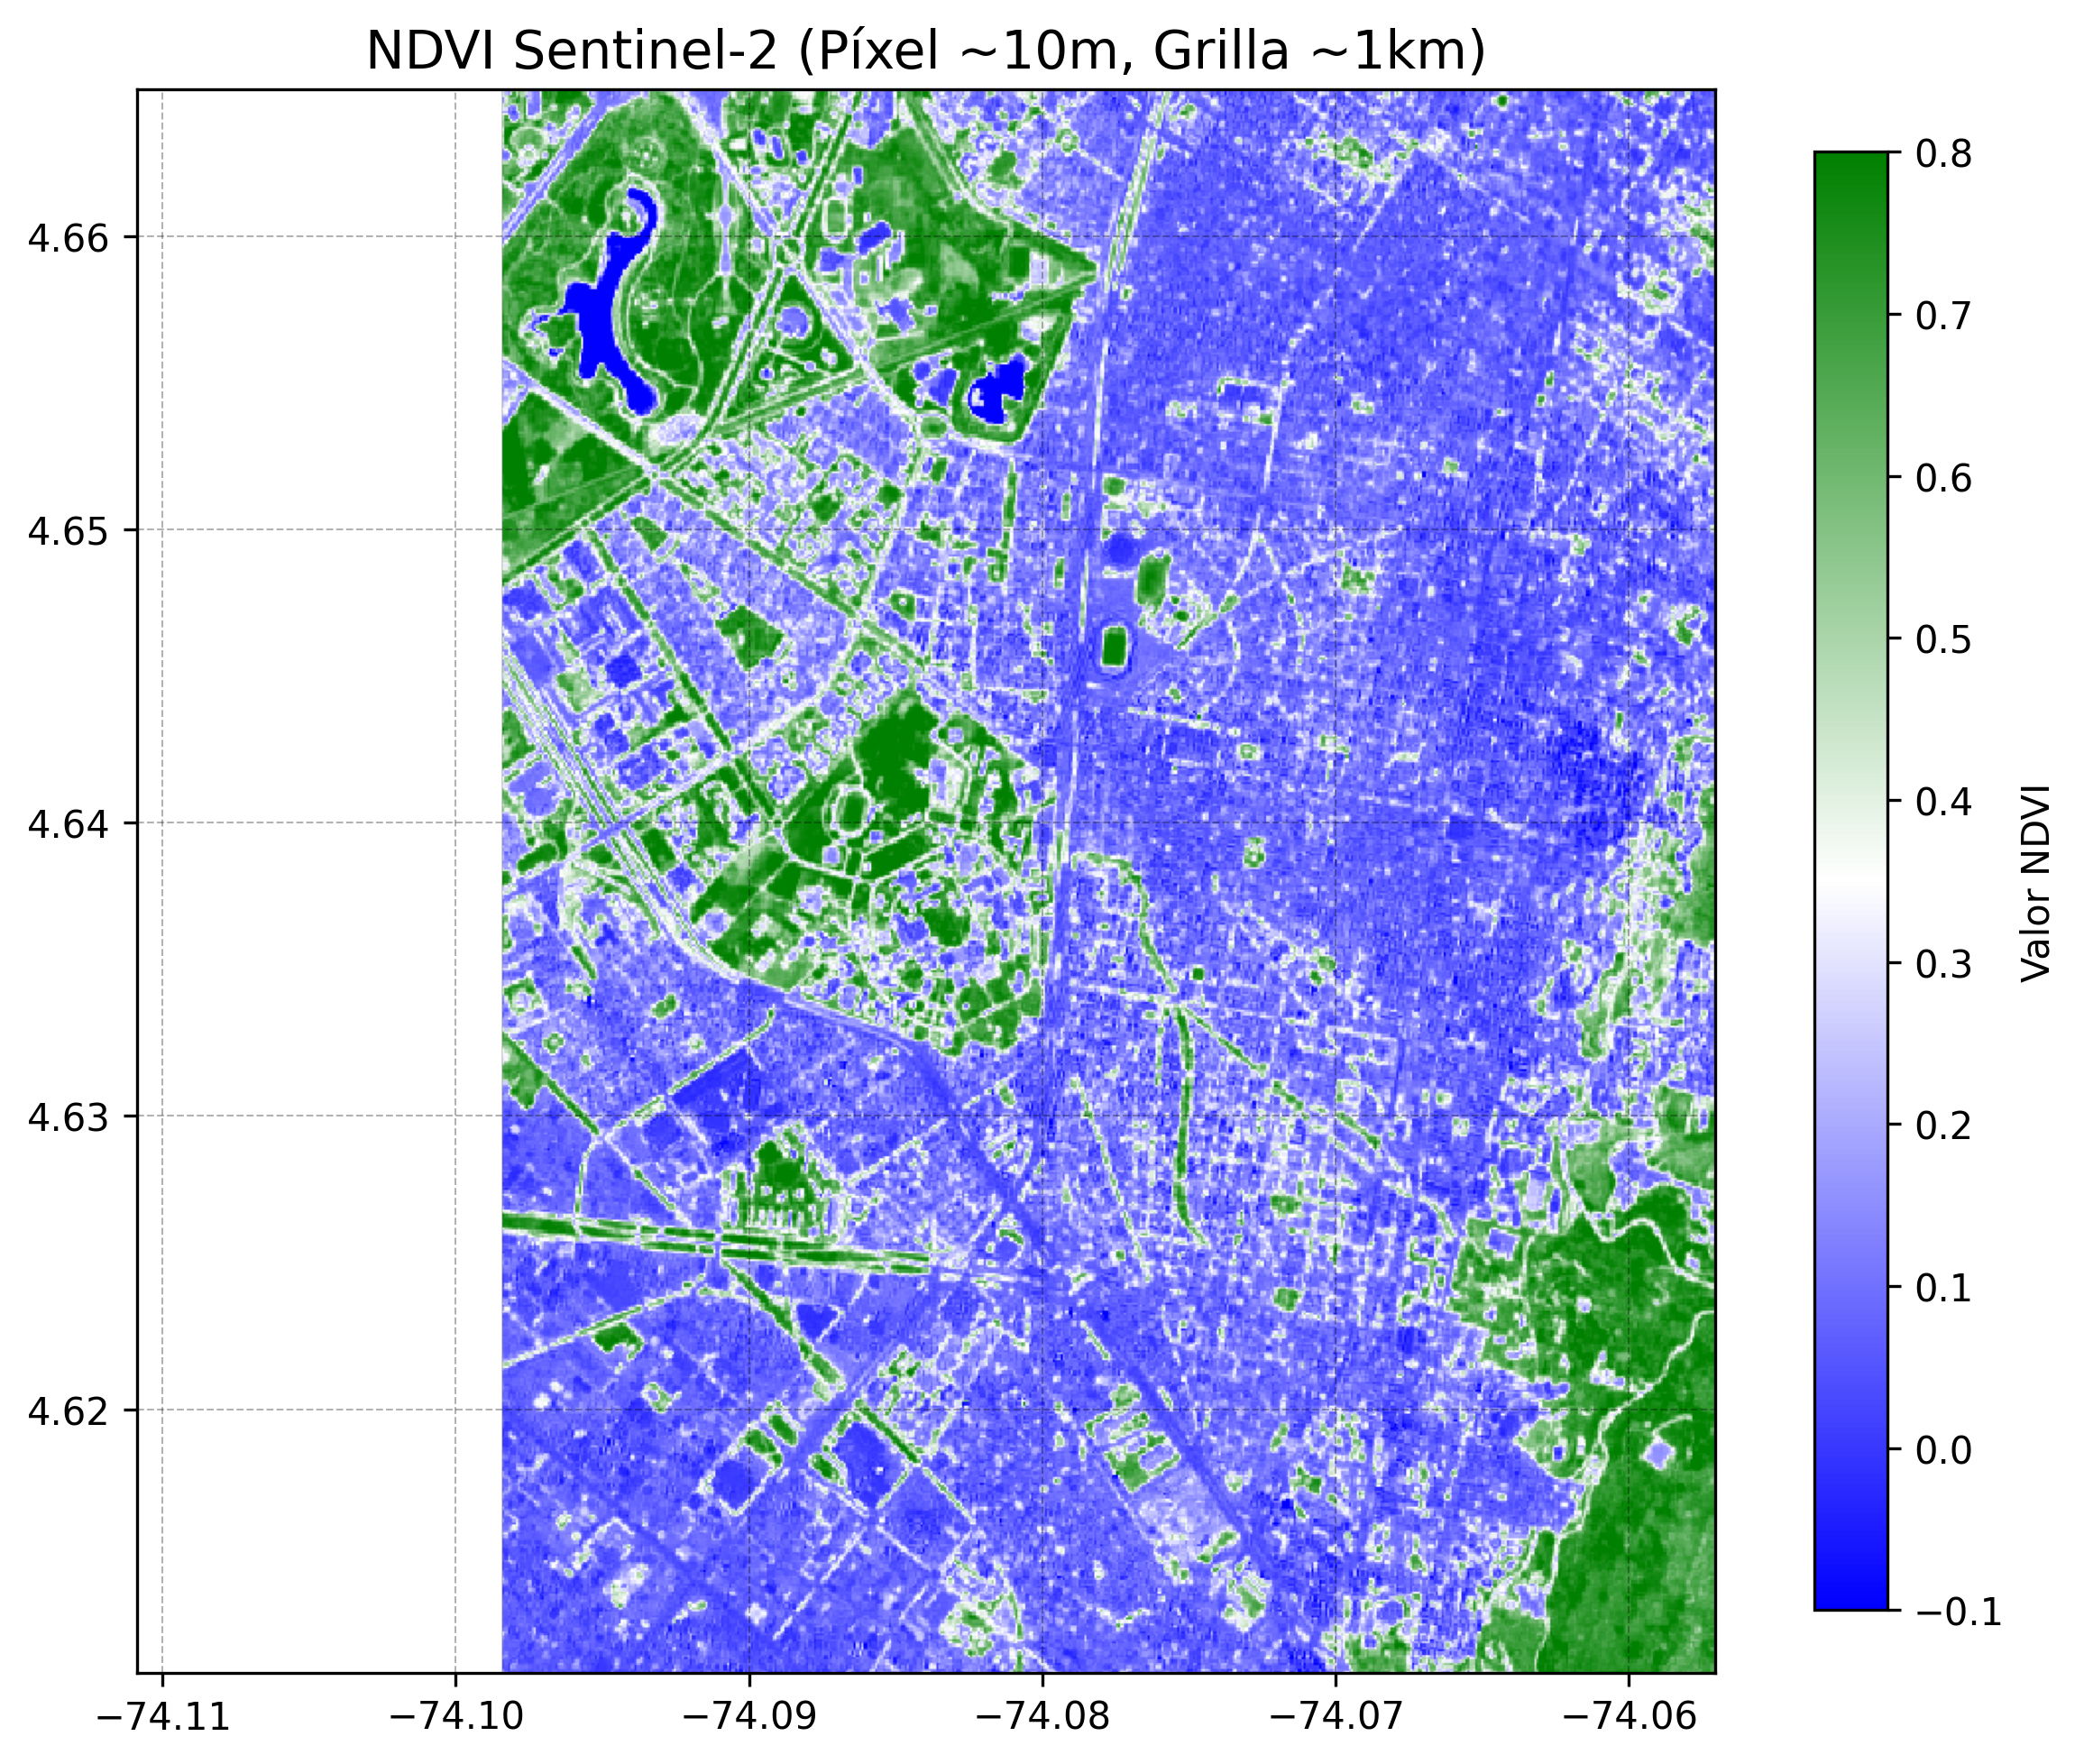
\includegraphics{45-practica_5_clase6_introduccion_sr_gee_files/figure-pdf/fig-python_ndvi_estatico-output-1.png}

}

\caption{\label{fig-python_ndvi_estatico}}

\end{figure}%

\subsection{Javascript}

Para ejecutar este código, debes abrir el
\textbf{\href{https://code.earthengine.google.com/}{Code Editor de
GEE}}.

\phantomsection\label{js_ndvi}%
\begin{Shaded}
\begin{Highlighting}[]
\CommentTok{// 1. CÁLCULO DEL ÍNDICE ESPECTRAL (NDVI)}
\KeywordTok{var}\NormalTok{ ndvi }\OperatorTok{=}\NormalTok{ s2\_clip}\OperatorTok{.}\FunctionTok{normalizedDifference}\NormalTok{([}\StringTok{\textquotesingle{}B8\textquotesingle{}}\OperatorTok{,} \StringTok{\textquotesingle{}B4\textquotesingle{}}\NormalTok{])}\OperatorTok{.}\FunctionTok{rename}\NormalTok{(}\StringTok{\textquotesingle{}NDVI\textquotesingle{}}\NormalTok{)}\OperatorTok{;}

\CommentTok{// 2. PARÁMETROS DE VISUALIZACIÓN}
\KeywordTok{var}\NormalTok{ vis\_ndvi }\OperatorTok{=}\NormalTok{ \{}\DataTypeTok{min}\OperatorTok{:} \OperatorTok{{-}}\FloatTok{0.1}\OperatorTok{,} \DataTypeTok{max}\OperatorTok{:} \FloatTok{0.8}\OperatorTok{,} \DataTypeTok{palette}\OperatorTok{:}\NormalTok{ [}\StringTok{\textquotesingle{}blue\textquotesingle{}}\OperatorTok{,} \StringTok{\textquotesingle{}white\textquotesingle{}}\OperatorTok{,} \StringTok{\textquotesingle{}green\textquotesingle{}}\NormalTok{]\}}\OperatorTok{;}

\CommentTok{// 3. MOSTRAR EN PANTALLA}
\BuiltInTok{Map}\OperatorTok{.}\FunctionTok{centerObject}\NormalTok{(ee}\OperatorTok{.}\AttributeTok{Geometry}\OperatorTok{.}\FunctionTok{Point}\NormalTok{([}\OperatorTok{{-}}\FloatTok{74.084}\OperatorTok{,} \FloatTok{4.638}\NormalTok{])}\OperatorTok{,} \DecValTok{17}\NormalTok{)}\OperatorTok{;}
\BuiltInTok{Map}\OperatorTok{.}\FunctionTok{addLayer}\NormalTok{(ndvi}\OperatorTok{,}\NormalTok{ vis\_ndvi}\OperatorTok{,} \StringTok{\textquotesingle{}NDVI Sentinel 2 {-} UNAL Bogotá\textquotesingle{}}\NormalTok{)}\OperatorTok{;}
\FunctionTok{print}\NormalTok{(}\StringTok{\textquotesingle{}NDVI procesado:\textquotesingle{}}\OperatorTok{,}\NormalTok{ ndvi)}\OperatorTok{;}
\end{Highlighting}
\end{Shaded}

\begin{center}\rule{0.5\linewidth}{0.5pt}\end{center}

\phantomsection\label{js_ndvi_estatico}%
\begin{Shaded}
\begin{Highlighting}[]
\CommentTok{// ▷ CÓDIGO MAPA ESTÁTICO (THUMBNAIL) EN JAVASCRIPT (Independiente)}
\KeywordTok{var}\NormalTok{ punto }\OperatorTok{=}\NormalTok{ ee}\OperatorTok{.}\AttributeTok{Geometry}\OperatorTok{.}\FunctionTok{Point}\NormalTok{([}\OperatorTok{{-}}\FloatTok{74.084}\OperatorTok{,} \FloatTok{4.638}\NormalTok{])}\OperatorTok{;}
\KeywordTok{var}\NormalTok{ s2\_img }\OperatorTok{=}\NormalTok{ ee}\OperatorTok{.}\FunctionTok{ImageCollection}\NormalTok{(}\StringTok{"COPERNICUS/S2\_SR\_HARMONIZED"}\NormalTok{)}\OperatorTok{.}\FunctionTok{filterBounds}\NormalTok{(punto)}\OperatorTok{.}\FunctionTok{filterDate}\NormalTok{(}\StringTok{\textquotesingle{}2023{-}01{-}01\textquotesingle{}}\OperatorTok{,} \StringTok{\textquotesingle{}2023{-}12{-}31\textquotesingle{}}\NormalTok{)}\OperatorTok{.}\FunctionTok{sort}\NormalTok{(}\StringTok{\textquotesingle{}CLOUDY\_PIXEL\_PERCENTAGE\textquotesingle{}}\NormalTok{)}\OperatorTok{.}\FunctionTok{first}\NormalTok{()}\OperatorTok{;}
\KeywordTok{var}\NormalTok{ ndvi\_thumb }\OperatorTok{=}\NormalTok{ s2\_img}\OperatorTok{.}\FunctionTok{normalizedDifference}\NormalTok{([}\StringTok{\textquotesingle{}B8\textquotesingle{}}\OperatorTok{,} \StringTok{\textquotesingle{}B4\textquotesingle{}}\NormalTok{])}\OperatorTok{;}

\KeywordTok{var}\NormalTok{ thumb\_params }\OperatorTok{=}\NormalTok{ \{}
  \DataTypeTok{min}\OperatorTok{:} \OperatorTok{{-}}\FloatTok{0.1}\OperatorTok{,} \DataTypeTok{max}\OperatorTok{:} \FloatTok{0.8}\OperatorTok{,}
  \DataTypeTok{palette}\OperatorTok{:}\NormalTok{ [}\StringTok{\textquotesingle{}blue\textquotesingle{}}\OperatorTok{,} \StringTok{\textquotesingle{}white\textquotesingle{}}\OperatorTok{,} \StringTok{\textquotesingle{}green\textquotesingle{}}\NormalTok{]}\OperatorTok{,}
  \DataTypeTok{dimensions}\OperatorTok{:} \DecValTok{800}\OperatorTok{,} \DataTypeTok{region}\OperatorTok{:}\NormalTok{ punto}\OperatorTok{.}\FunctionTok{buffer}\NormalTok{(}\DecValTok{3000}\NormalTok{)}
\NormalTok{\}}\OperatorTok{;}

\FunctionTok{print}\NormalTok{(}\StringTok{\textquotesingle{}Miniatura NDVI (Valores {-}0.1 a 0.8):\textquotesingle{}}\OperatorTok{,}\NormalTok{ ui}\OperatorTok{.}\FunctionTok{Thumbnail}\NormalTok{(\{}\DataTypeTok{image}\OperatorTok{:}\NormalTok{ ndvi\_thumb}\OperatorTok{,} \DataTypeTok{params}\OperatorTok{:}\NormalTok{ thumb\_params}\OperatorTok{,} \DataTypeTok{style}\OperatorTok{:}\NormalTok{ \{}\DataTypeTok{width}\OperatorTok{:} \StringTok{\textquotesingle{}400px\textquotesingle{}}\NormalTok{\}\}))}\OperatorTok{;}
\end{Highlighting}
\end{Shaded}

\begin{center}\rule{0.5\linewidth}{0.5pt}\end{center}

\subsection{Reto: Carga del índice espectral en QGIS y ArcGIS
Pro}\label{reto-carga-del-uxedndice-espectral-en-qgis-y-arcgis-pro}

Proceda a importar el resultado del álgebra de mapas en su entorno SIG
de escritorio. Dado que el NDVI es un cálculo matemático en vivo y no un
archivo preexistente en el catálogo de Google, no tiene un \emph{Asset
ID} directo.

\textbf{Instrucciones:}

\begin{enumerate}
\def\labelenumi{\arabic{enumi}.}
\tightlist
\item
  Ejecute el código de Python correspondiente para calcular el NDVI y
  generar el archivo \texttt{ndvi\_serializado.json}.
\item
  En \textbf{ArcGIS Pro}, utilice la herramienta \emph{Add Image to Map
  by Serialized Object}. El plugin leerá la instrucción serializada y le
  pedirá a los servidores de Google que ejecuten el cálculo del NDVI
  antes de enviarlo a su pantalla.
\item
  En \textbf{QGIS}, debido a que la pestaña \emph{Load} no procesa
  cálculos, debe utilizar la pestaña \textbf{Code} y ejecutar
  directamente el script de Python que generamos (asegúrese de incluir
  la carga previa de \texttt{s2\_clip} en el mismo script).
\item
  \textbf{Reporte:} Capture la pantalla de las herramientas o de la
  ejecución del código antes de procesarlo e insértelas a continuación.
\end{enumerate}

\begin{quote}
\textbf{Reporte visual de NDVI}

\emph{Captura de QGIS (Pestaña Code ejecutando el NDVI):}
\texttt{!{[}Parámetros\ de\ NDVI\ en\ QGIS{]}(ruta/a/tu/captura\_qgis\_ndvi.png)\{fig-align="center"\ width="80\%"\}}

\emph{Captura de ArcGIS Pro (Herramienta utilizada con el archivo
JSON):}
\texttt{!{[}Parámetros\ de\ NDVI\ en\ ArcGIS\ Pro{]}(ruta/a/tu/captura\_arcgis\_ndvi.png)\{fig-align="center"\ width="80\%"\}}
\end{quote}

\section{Análisis temporal y galería
visual}\label{anuxe1lisis-temporal-y-galeruxeda-visual}

El análisis de series temporales permite observar la evolución de
variables biofísicas. En esta sección generaremos la curva de NDVI para
Bogotá D.C. y extraeremos una tira de imágenes (\emph{filmstrip}) para
verificar visualmente los cambios en la cobertura vegetal.

\[NDVI = \frac{NIR - Red}{NIR + Red}\]

\subsection{Python}

\begin{Shaded}
\begin{Highlighting}[]
\CommentTok{\# \#| echo: false}
\CommentTok{\# \#| eval: false}

\ImportTok{import}\NormalTok{ ee}
\ImportTok{import}\NormalTok{ pandas }\ImportTok{as}\NormalTok{ pd}
\ImportTok{import}\NormalTok{ matplotlib.pyplot }\ImportTok{as}\NormalTok{ plt}
\ImportTok{import}\NormalTok{ datetime}
\ImportTok{import}\NormalTok{ urllib.request}
\ImportTok{from}\NormalTok{ PIL }\ImportTok{import}\NormalTok{ Image}
\ImportTok{import}\NormalTok{ numpy }\ImportTok{as}\NormalTok{ np}

\CommentTok{\# 1. DEFINICIÓN DEL ÁREA}
\NormalTok{localidades }\OperatorTok{=}\NormalTok{ ee.FeatureCollection(}\StringTok{"FAO/GAUL/2015/level2"}\NormalTok{)}
\NormalTok{bogota }\OperatorTok{=}\NormalTok{ localidades.}\BuiltInTok{filter}\NormalTok{(ee.Filter.eq(}\StringTok{\textquotesingle{}ADM2\_NAME\textquotesingle{}}\NormalTok{, }\StringTok{\textquotesingle{}Santafe De Bogota D.c.\textquotesingle{}}\NormalTok{))}

\CommentTok{\# 2. PROCESAMIENTO}
\NormalTok{s2\_ts }\OperatorTok{=}\NormalTok{ (ee.ImageCollection(}\StringTok{"COPERNICUS/S2\_SR\_HARMONIZED"}\NormalTok{)}
\NormalTok{    .filterBounds(bogota)}
\NormalTok{    .filterDate(}\StringTok{\textquotesingle{}2023{-}01{-}01\textquotesingle{}}\NormalTok{, }\StringTok{\textquotesingle{}2023{-}12{-}31\textquotesingle{}}\NormalTok{)}
\NormalTok{    .}\BuiltInTok{filter}\NormalTok{(ee.Filter.lt(}\StringTok{\textquotesingle{}CLOUDY\_PIXEL\_PERCENTAGE\textquotesingle{}}\NormalTok{, }\DecValTok{15}\NormalTok{))}
\NormalTok{    .select([}\StringTok{\textquotesingle{}B8\textquotesingle{}}\NormalTok{, }\StringTok{\textquotesingle{}B4\textquotesingle{}}\NormalTok{, }\StringTok{\textquotesingle{}B3\textquotesingle{}}\NormalTok{, }\StringTok{\textquotesingle{}B2\textquotesingle{}}\NormalTok{]))}

\KeywordTok{def}\NormalTok{ add\_ndvi(img):}
\NormalTok{    ndvi }\OperatorTok{=}\NormalTok{ img.normalizedDifference([}\StringTok{\textquotesingle{}B8\textquotesingle{}}\NormalTok{, }\StringTok{\textquotesingle{}B4\textquotesingle{}}\NormalTok{]).rename(}\StringTok{\textquotesingle{}NDVI\textquotesingle{}}\NormalTok{)}
    \ControlFlowTok{return}\NormalTok{ img.addBands(ndvi).copyProperties(img, [}\StringTok{\textquotesingle{}system:time\_start\textquotesingle{}}\NormalTok{])}

\NormalTok{s2\_ndvi }\OperatorTok{=}\NormalTok{ s2\_ts.}\BuiltInTok{map}\NormalTok{(add\_ndvi)}

\KeywordTok{def}\NormalTok{ extract\_ndvi(img):}
\NormalTok{    mean\_dict }\OperatorTok{=}\NormalTok{ img.reduceRegion(reducer}\OperatorTok{=}\NormalTok{ee.Reducer.mean(), geometry}\OperatorTok{=}\NormalTok{bogota.geometry(), scale}\OperatorTok{=}\DecValTok{500}\NormalTok{, maxPixels}\OperatorTok{=}\FloatTok{1e9}\NormalTok{)}
    \ControlFlowTok{return}\NormalTok{ ee.Feature(}\VariableTok{None}\NormalTok{, \{}\StringTok{\textquotesingle{}NDVI\textquotesingle{}}\NormalTok{: mean\_dict.get(}\StringTok{\textquotesingle{}NDVI\textquotesingle{}}\NormalTok{), }\StringTok{\textquotesingle{}system:time\_start\textquotesingle{}}\NormalTok{: img.get(}\StringTok{\textquotesingle{}system:time\_start\textquotesingle{}}\NormalTok{)\})}

\NormalTok{ndvi\_features }\OperatorTok{=}\NormalTok{ ee.FeatureCollection(s2\_ndvi.}\BuiltInTok{map}\NormalTok{(extract\_ndvi)).}\BuiltInTok{filter}\NormalTok{(ee.Filter.notNull([}\StringTok{\textquotesingle{}NDVI\textquotesingle{}}\NormalTok{]))}
\NormalTok{ndvi\_list }\OperatorTok{=}\NormalTok{ ndvi\_features.reduceColumns(ee.Reducer.toList(}\DecValTok{2}\NormalTok{), [}\StringTok{\textquotesingle{}system:time\_start\textquotesingle{}}\NormalTok{, }\StringTok{\textquotesingle{}NDVI\textquotesingle{}}\NormalTok{]).get(}\StringTok{\textquotesingle{}list\textquotesingle{}}\NormalTok{).getInfo()}

\NormalTok{df }\OperatorTok{=}\NormalTok{ pd.DataFrame(ndvi\_list, columns}\OperatorTok{=}\NormalTok{[}\StringTok{\textquotesingle{}Time\textquotesingle{}}\NormalTok{, }\StringTok{\textquotesingle{}NDVI\textquotesingle{}}\NormalTok{])}
\NormalTok{df[}\StringTok{\textquotesingle{}Time\textquotesingle{}}\NormalTok{] }\OperatorTok{=}\NormalTok{ pd.to\_datetime(df[}\StringTok{\textquotesingle{}Time\textquotesingle{}}\NormalTok{], unit}\OperatorTok{=}\StringTok{\textquotesingle{}ms\textquotesingle{}}\NormalTok{)}
\NormalTok{df }\OperatorTok{=}\NormalTok{ df.sort\_values(}\StringTok{\textquotesingle{}Time\textquotesingle{}}\NormalTok{)}

\CommentTok{\# 3. VISUALIZACIÓN (Matplotlib)}
\NormalTok{fig }\OperatorTok{=}\NormalTok{ plt.figure(figsize}\OperatorTok{=}\NormalTok{(}\DecValTok{12}\NormalTok{, }\DecValTok{10}\NormalTok{))}
\NormalTok{ax1 }\OperatorTok{=}\NormalTok{ plt.subplot2grid((}\DecValTok{3}\NormalTok{, }\DecValTok{1}\NormalTok{), (}\DecValTok{0}\NormalTok{, }\DecValTok{0}\NormalTok{), rowspan}\OperatorTok{=}\DecValTok{2}\NormalTok{)}
\NormalTok{ax1.plot(df[}\StringTok{\textquotesingle{}Time\textquotesingle{}}\NormalTok{], df[}\StringTok{\textquotesingle{}NDVI\textquotesingle{}}\NormalTok{], marker}\OperatorTok{=}\StringTok{\textquotesingle{}o\textquotesingle{}}\NormalTok{, color}\OperatorTok{=}\StringTok{\textquotesingle{}\#228B22\textquotesingle{}}\NormalTok{, linewidth}\OperatorTok{=}\DecValTok{2}\NormalTok{)}
\NormalTok{ax1.set\_title(}\StringTok{\textquotesingle{}Serie temporal NDVI {-} Bogotá D.C. (2023)\textquotesingle{}}\NormalTok{)}
\NormalTok{ax1.grid(}\VariableTok{True}\NormalTok{, linestyle}\OperatorTok{=}\StringTok{\textquotesingle{}{-}{-}\textquotesingle{}}\NormalTok{, alpha}\OperatorTok{=}\FloatTok{0.6}\NormalTok{)}

\NormalTok{n\_thumbs }\OperatorTok{=} \DecValTok{5}
\NormalTok{img\_list }\OperatorTok{=}\NormalTok{ s2\_ts.sort(}\StringTok{\textquotesingle{}system:time\_start\textquotesingle{}}\NormalTok{).toList(n\_thumbs)}
\NormalTok{count }\OperatorTok{=}\NormalTok{ img\_list.size().getInfo()}

\ControlFlowTok{for}\NormalTok{ i }\KeywordTok{in} \BuiltInTok{range}\NormalTok{(}\BuiltInTok{min}\NormalTok{(n\_thumbs, count)):}
\NormalTok{    img }\OperatorTok{=}\NormalTok{ ee.Image(img\_list.get(i))}
\NormalTok{    fecha\_ms }\OperatorTok{=}\NormalTok{ img.get(}\StringTok{\textquotesingle{}system:time\_start\textquotesingle{}}\NormalTok{).getInfo()}
\NormalTok{    fecha }\OperatorTok{=}\NormalTok{ datetime.datetime.fromtimestamp(fecha\_ms }\OperatorTok{/} \FloatTok{1000.0}\NormalTok{, datetime.UTC).strftime(}\StringTok{\textquotesingle{}\%Y{-}\%m{-}}\SpecialCharTok{\%d}\StringTok{\textquotesingle{}}\NormalTok{)}
    
\NormalTok{    thumb\_url }\OperatorTok{=}\NormalTok{ img.getThumbURL(\{}
        \StringTok{\textquotesingle{}bands\textquotesingle{}}\NormalTok{: [}\StringTok{\textquotesingle{}B4\textquotesingle{}}\NormalTok{, }\StringTok{\textquotesingle{}B3\textquotesingle{}}\NormalTok{, }\StringTok{\textquotesingle{}B2\textquotesingle{}}\NormalTok{], }\StringTok{\textquotesingle{}min\textquotesingle{}}\NormalTok{: }\DecValTok{0}\NormalTok{, }\StringTok{\textquotesingle{}max\textquotesingle{}}\NormalTok{: }\DecValTok{3000}\NormalTok{,}
        \StringTok{\textquotesingle{}dimensions\textquotesingle{}}\NormalTok{: }\DecValTok{300}\NormalTok{, }\StringTok{\textquotesingle{}region\textquotesingle{}}\NormalTok{: bogota.geometry().bounds(), }\StringTok{\textquotesingle{}format\textquotesingle{}}\NormalTok{: }\StringTok{\textquotesingle{}png\textquotesingle{}}
\NormalTok{    \})}
    
    \ControlFlowTok{with}\NormalTok{ urllib.request.urlopen(thumb\_url) }\ImportTok{as}\NormalTok{ url\_response:}
\NormalTok{        img\_array }\OperatorTok{=}\NormalTok{ np.array(Image.}\BuiltInTok{open}\NormalTok{(url\_response))}
    
\NormalTok{    ax\_thumb }\OperatorTok{=}\NormalTok{ plt.subplot2grid((}\DecValTok{3}\NormalTok{, n\_thumbs), (}\DecValTok{2}\NormalTok{, i))}
\NormalTok{    ax\_thumb.imshow(img\_array)}
\NormalTok{    ax\_thumb.set\_title(fecha, fontsize}\OperatorTok{=}\DecValTok{9}\NormalTok{)}
\NormalTok{    ax\_thumb.axis(}\StringTok{\textquotesingle{}off\textquotesingle{}}\NormalTok{)}

\NormalTok{plt.tight\_layout()}
\NormalTok{plt.show()}
\end{Highlighting}
\end{Shaded}

\begin{figure}[H]

\centering{

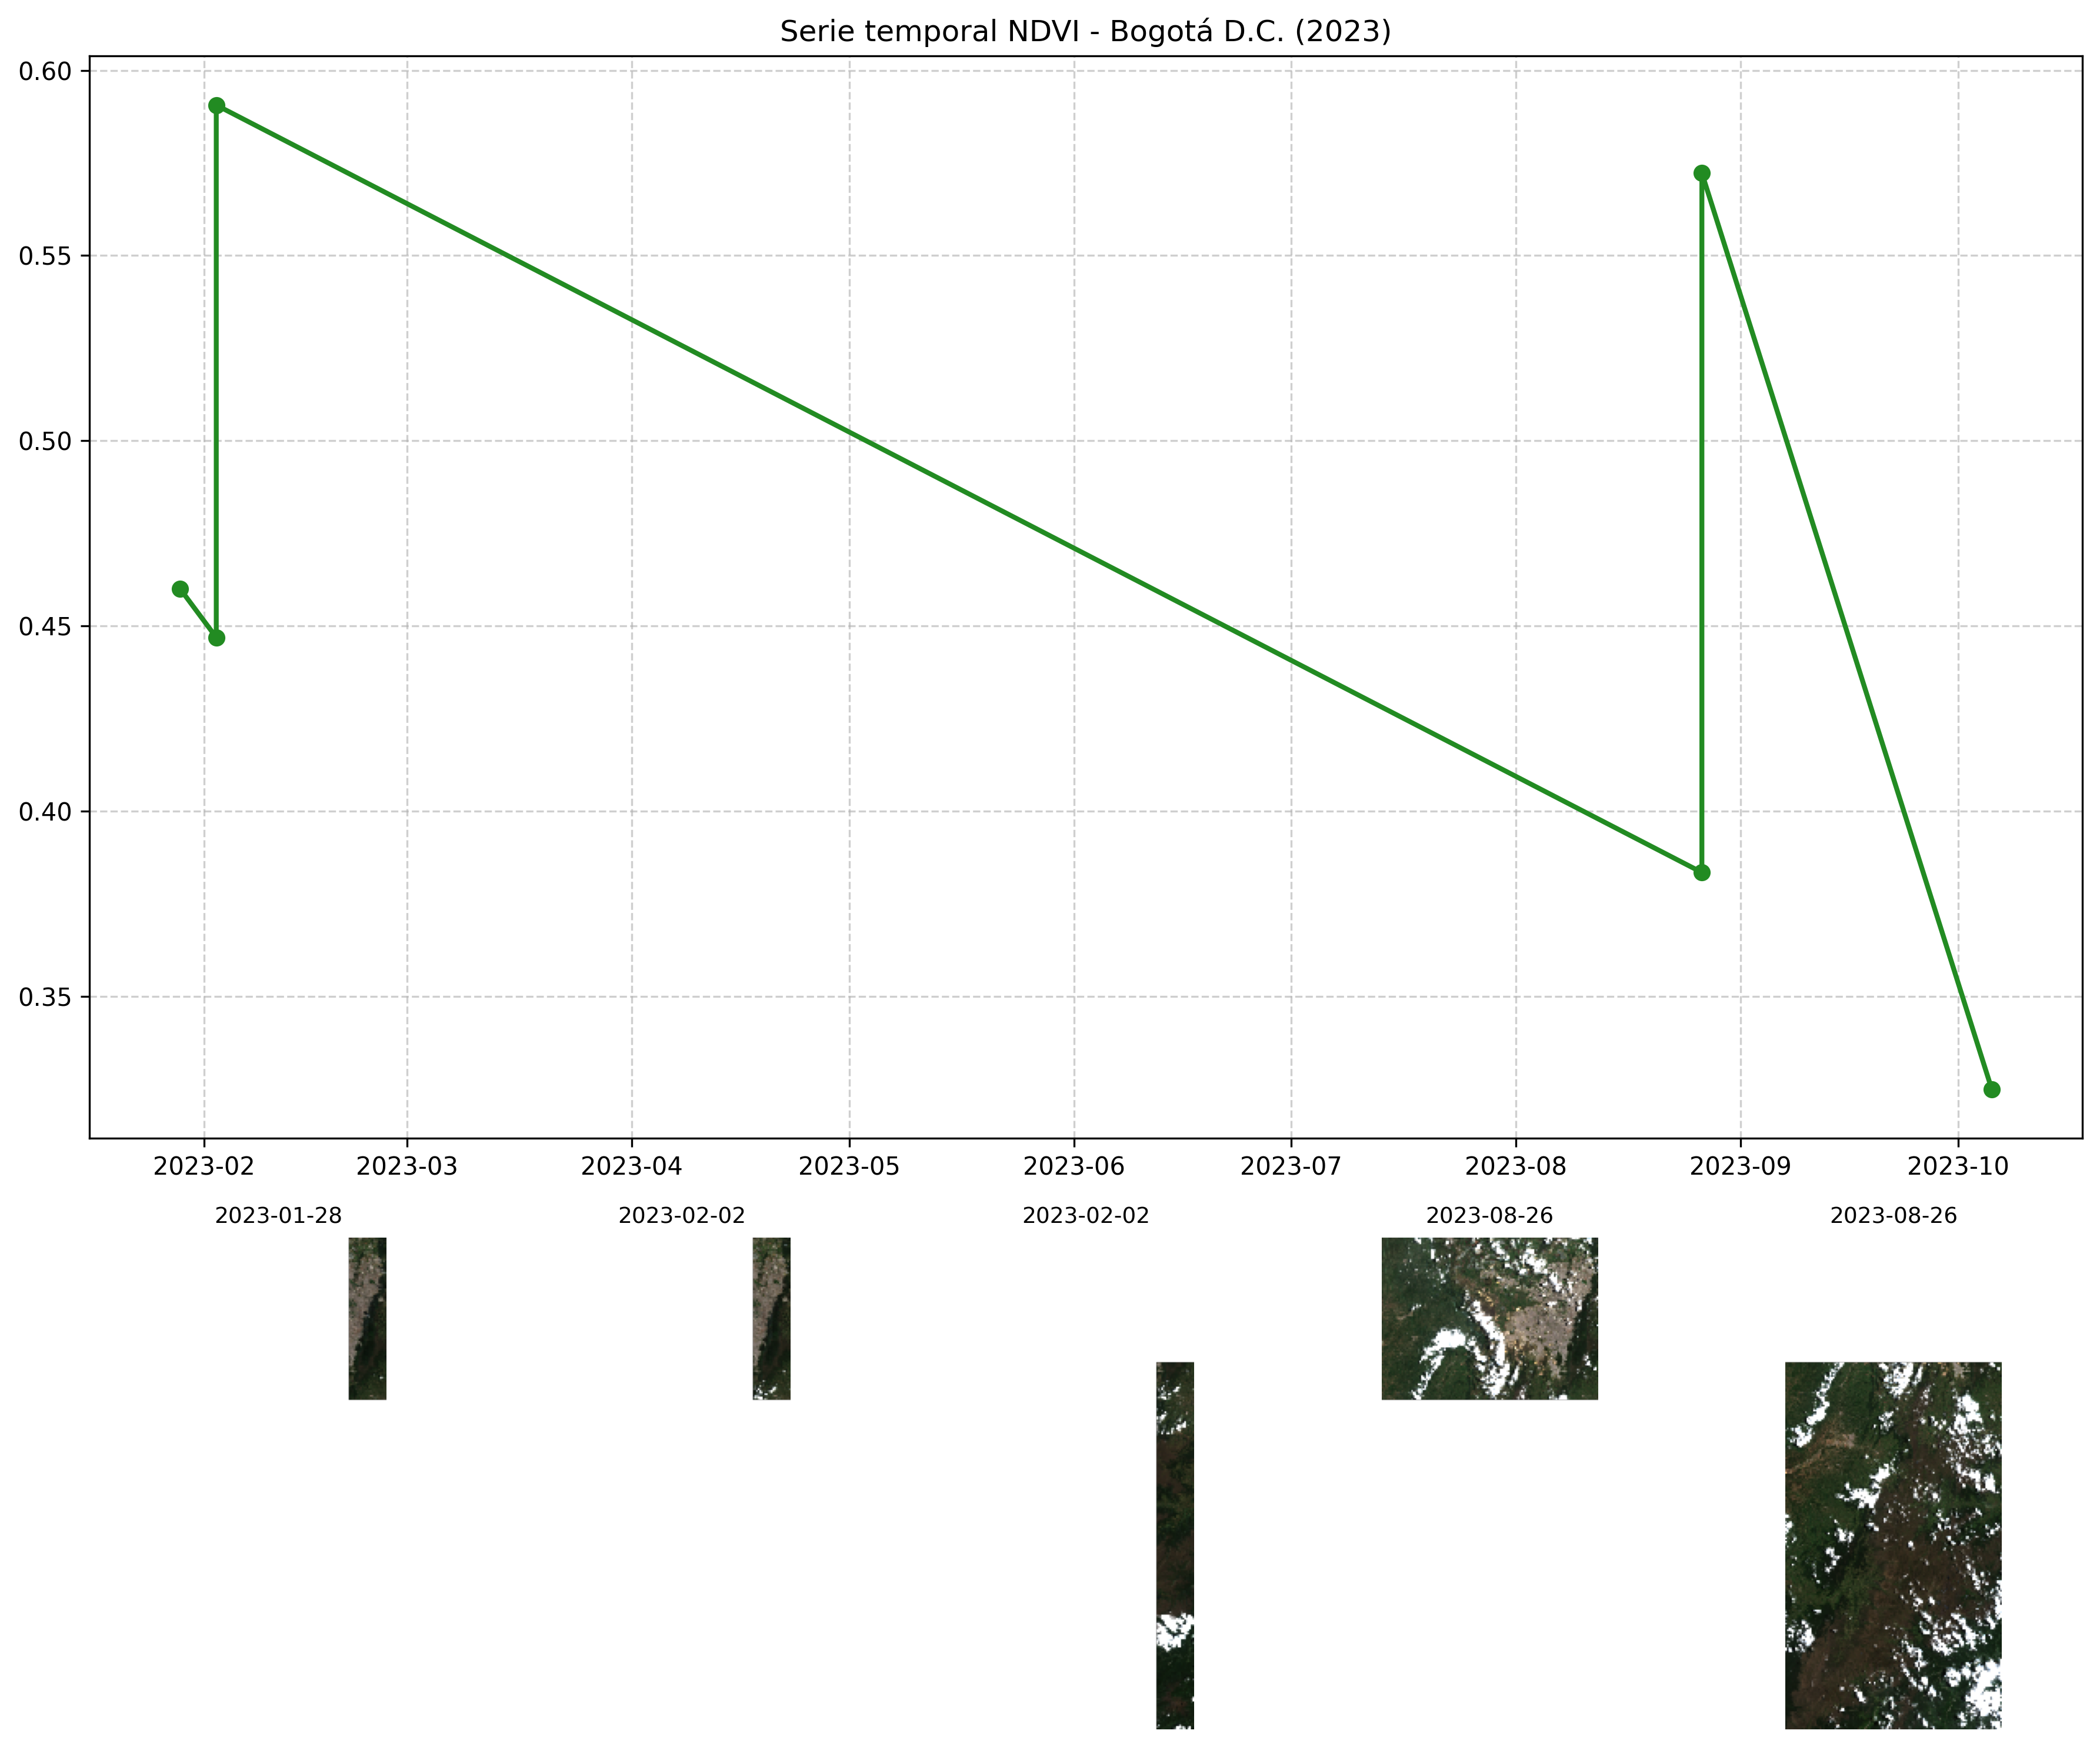
\includegraphics{45-practica_5_clase6_introduccion_sr_gee_files/figure-pdf/fig-temporal-output-1.png}

}

\caption{\label{fig-temporal}Serie temporal del Índice de Vegetación
(NDVI) para Bogotá D.C. durante 2023, acompañada de galería de imágenes
(Filmstrip) en color verdadero.}

\end{figure}%

\subsection{Javascript}

Para ejecutar este código, debes abrir el
\textbf{\href{https://code.earthengine.google.com/}{Code Editor de
Google Earth Engine}}, pegar el fragmento y hacer clic en
\textbf{``Run''}.

\phantomsection\label{js_temporal_gallery}%
\begin{Shaded}
\begin{Highlighting}[]
\KeywordTok{var}\NormalTok{ bogota }\OperatorTok{=}\NormalTok{ ee}\OperatorTok{.}\FunctionTok{FeatureCollection}\NormalTok{(}\StringTok{"FAO/GAUL/2015/level2"}\NormalTok{)}
  \OperatorTok{.}\FunctionTok{filter}\NormalTok{(ee}\OperatorTok{.}\AttributeTok{Filter}\OperatorTok{.}\FunctionTok{eq}\NormalTok{(}\StringTok{\textquotesingle{}ADM2\_NAME\textquotesingle{}}\OperatorTok{,} \StringTok{\textquotesingle{}Santafe De Bogota D.c.\textquotesingle{}}\NormalTok{))}\OperatorTok{;}

\KeywordTok{var}\NormalTok{ s2\_ts }\OperatorTok{=}\NormalTok{ ee}\OperatorTok{.}\FunctionTok{ImageCollection}\NormalTok{(}\StringTok{"COPERNICUS/S2\_SR\_HARMONIZED"}\NormalTok{)}
  \OperatorTok{.}\FunctionTok{filterBounds}\NormalTok{(bogota)}
  \OperatorTok{.}\FunctionTok{filterDate}\NormalTok{(}\StringTok{\textquotesingle{}2023{-}01{-}01\textquotesingle{}}\OperatorTok{,} \StringTok{\textquotesingle{}2023{-}12{-}31\textquotesingle{}}\NormalTok{)}
  \OperatorTok{.}\FunctionTok{filter}\NormalTok{(ee}\OperatorTok{.}\AttributeTok{Filter}\OperatorTok{.}\FunctionTok{lt}\NormalTok{(}\StringTok{\textquotesingle{}CLOUDY\_PIXEL\_PERCENTAGE\textquotesingle{}}\OperatorTok{,} \DecValTok{15}\NormalTok{))}\OperatorTok{;}

\KeywordTok{var}\NormalTok{ s2\_ndvi }\OperatorTok{=}\NormalTok{ s2\_ts}\OperatorTok{.}\FunctionTok{map}\NormalTok{(}\KeywordTok{function}\NormalTok{(img) \{}
  \KeywordTok{var}\NormalTok{ ndvi }\OperatorTok{=}\NormalTok{ img}\OperatorTok{.}\FunctionTok{normalizedDifference}\NormalTok{([}\StringTok{\textquotesingle{}B8\textquotesingle{}}\OperatorTok{,} \StringTok{\textquotesingle{}B4\textquotesingle{}}\NormalTok{])}\OperatorTok{.}\FunctionTok{rename}\NormalTok{(}\StringTok{\textquotesingle{}NDVI\textquotesingle{}}\NormalTok{)}\OperatorTok{;}
  \ControlFlowTok{return}\NormalTok{ img}\OperatorTok{.}\FunctionTok{addBands}\NormalTok{(ndvi)}\OperatorTok{.}\FunctionTok{copyProperties}\NormalTok{(img}\OperatorTok{,}\NormalTok{ [}\StringTok{\textquotesingle{}system:time\_start\textquotesingle{}}\NormalTok{])}\OperatorTok{;}
\NormalTok{\})}\OperatorTok{;}

\FunctionTok{print}\NormalTok{(ui}\OperatorTok{.}\AttributeTok{Chart}\OperatorTok{.}\AttributeTok{image}\OperatorTok{.}\FunctionTok{series}\NormalTok{(s2\_ndvi}\OperatorTok{.}\FunctionTok{select}\NormalTok{(}\StringTok{\textquotesingle{}NDVI\textquotesingle{}}\NormalTok{)}\OperatorTok{,}\NormalTok{ bogota}\OperatorTok{,}\NormalTok{ ee}\OperatorTok{.}\AttributeTok{Reducer}\OperatorTok{.}\FunctionTok{mean}\NormalTok{()}\OperatorTok{,} \DecValTok{500}\NormalTok{))}\OperatorTok{;}

\KeywordTok{var}\NormalTok{ gallery }\OperatorTok{=}\NormalTok{ s2\_ts}\OperatorTok{.}\FunctionTok{sort}\NormalTok{(}\StringTok{\textquotesingle{}system:time\_start\textquotesingle{}}\NormalTok{)}\OperatorTok{.}\FunctionTok{toList}\NormalTok{(}\DecValTok{5}\NormalTok{)}\OperatorTok{;}
\NormalTok{gallery}\OperatorTok{.}\FunctionTok{evaluate}\NormalTok{(}\KeywordTok{function}\NormalTok{(list) \{}
\NormalTok{  list}\OperatorTok{.}\FunctionTok{forEach}\NormalTok{(}\KeywordTok{function}\NormalTok{(img\_metadata) \{}
    \KeywordTok{var}\NormalTok{ img }\OperatorTok{=}\NormalTok{ ee}\OperatorTok{.}\FunctionTok{Image}\NormalTok{(img\_metadata}\OperatorTok{.}\AttributeTok{id}\NormalTok{)}\OperatorTok{;}
    \KeywordTok{var}\NormalTok{ fecha }\OperatorTok{=} \KeywordTok{new} \BuiltInTok{Date}\NormalTok{(img\_metadata}\OperatorTok{.}\AttributeTok{properties}\NormalTok{[}\StringTok{\textquotesingle{}system:time\_start\textquotesingle{}}\NormalTok{])}\OperatorTok{.}\FunctionTok{toISOString}\NormalTok{()}\OperatorTok{.}\FunctionTok{split}\NormalTok{(}\StringTok{\textquotesingle{}T\textquotesingle{}}\NormalTok{)[}\DecValTok{0}\NormalTok{]}\OperatorTok{;}
    \FunctionTok{print}\NormalTok{(fecha}\OperatorTok{,}\NormalTok{ ui}\OperatorTok{.}\FunctionTok{Thumbnail}\NormalTok{(\{}
      \DataTypeTok{image}\OperatorTok{:}\NormalTok{ img}\OperatorTok{,}
      \DataTypeTok{params}\OperatorTok{:}\NormalTok{ \{}\DataTypeTok{bands}\OperatorTok{:}\NormalTok{ [}\StringTok{\textquotesingle{}B4\textquotesingle{}}\OperatorTok{,} \StringTok{\textquotesingle{}B3\textquotesingle{}}\OperatorTok{,} \StringTok{\textquotesingle{}B2\textquotesingle{}}\NormalTok{]}\OperatorTok{,} \DataTypeTok{min}\OperatorTok{:} \DecValTok{0}\OperatorTok{,} \DataTypeTok{max}\OperatorTok{:} \DecValTok{3000}\OperatorTok{,} \DataTypeTok{region}\OperatorTok{:}\NormalTok{ bogota}\OperatorTok{.}\FunctionTok{geometry}\NormalTok{()}\OperatorTok{.}\FunctionTok{bounds}\NormalTok{()\}}\OperatorTok{,}
      \DataTypeTok{style}\OperatorTok{:}\NormalTok{ \{}\DataTypeTok{width}\OperatorTok{:} \StringTok{\textquotesingle{}200px\textquotesingle{}}\NormalTok{\}}
\NormalTok{    \}))}\OperatorTok{;}
\NormalTok{  \})}\OperatorTok{;}
\NormalTok{\})}\OperatorTok{;}
\end{Highlighting}
\end{Shaded}

\begin{center}\rule{0.5\linewidth}{0.5pt}\end{center}

\subsection{Interpretación de resultados: ¿Por qué la variabilidad
visual?}\label{interpretaciuxf3n-de-resultados-por-quuxe9-la-variabilidad-visual}

Al observar la serie temporal y su respectiva galería de imágenes, es
común notar discrepancias visuales significativas. No se trata de un
error en el código, sino de la naturaleza misma de la teledetección
óptica.

\subsubsection{La anatomía de una serie temporal
satelital}\label{la-anatomuxeda-de-una-serie-temporal-satelital}

Lo que estamos haciendo es transformar una \textbf{Colección de
Imágenes} (datos crudos) en un \textbf{Gráfico Estadístico}
(información). Sin embargo, esa transición no siempre es lineal debido a
tres factores principales:

\begin{itemize}
\tightlist
\item
  \textbf{Efecto de las nubes:} Aunque aplicamos un filtro del 15\%, las
  nubes son caprichosas. En Bogotá, una imagen puede tener un 10\% de
  nubes concentradas justo sobre el área urbana, mientras que otra puede
  tener el mismo porcentaje distribuido en los cerros orientales.
\item
  \textbf{Geometría de captura (Tiles):} Sentinel-2 divide el mundo en
  cuadrículas estandarizadas. Dependiendo del día de la órbita, Bogotá
  puede quedar en el centro de una toma o en el borde de otra, lo que
  explica por qué algunas miniaturas parecen ``recortadas''.
\item
  \textbf{Condiciones atmosféricas:} El ``ruido'' causado por la
  humedad, el esmog o el ángulo de iluminación solar según la estación
  cambia el brillo de la imagen, aunque el sensor sea el mismo.
\end{itemize}

\subsubsection{¿Cómo interfieren las nubes en el
NDVI?}\label{cuxf3mo-interfieren-las-nubes-en-el-ndvi}

Las nubes son el mayor enemigo del analista óptico. Físicamente, una
nube tiene una alta reflectancia tanto en el Infrarrojo Cercano
(\(NIR\)) como en el Rojo (\(Red\)).

\[NDVI_{nube} \approx \frac{Alto - Alto}{Alto + Alto} \approx 0\]

Cuando el algoritmo calcula el promedio para todo el polígono de Bogotá:

\begin{enumerate}
\def\labelenumi{\arabic{enumi}.}
\tightlist
\item
  Si la imagen está limpia, el NDVI refleja el verdor real de los
  parques y cerros (valores altos).
\item
  Si hay nubes residuales, el valor de esos píxeles (cercanos a 0)
  ``tira hacia abajo'' el promedio general.
\item
  \textbf{Resultado:} Verás valles profundos en la gráfica que no
  representan una pérdida de vegetación, sino la presencia de cobertura
  nubosa que ``engañó'' al promedio.
\end{enumerate}

\begin{quote}
\textbf{Nota de experto:} Esta es la razón por la cual nunca debemos
confiar en un dato estadístico satelital sin verificar su respaldo
visual en la galería (\emph{filmstrip}).
\end{quote}

\subsection{Reto: Análisis de la serie temporal y la galería
visual}\label{reto-anuxe1lisis-de-la-serie-temporal-y-la-galeruxeda-visual}

Compare los resultados numéricos de la gráfica con la evidencia visual
de las miniaturas.

\textbf{Instrucciones:}

\begin{enumerate}
\def\labelenumi{\arabic{enumi}.}
\tightlist
\item
  Ejecute el bloque de Python y observe la tendencia anual en la gráfica
  generada por Quarto.
\item
  Identifique si las variaciones bruscas en el NDVI corresponden a
  cambios reales o a nubosidad residual visible en el \emph{filmstrip}.
\item
  \textbf{Reporte:} Tome una captura de pantalla del resultado combinado
  (Gráfica + Galería) e insértela a continuación.
\end{enumerate}

\begin{quote}
\textbf{Reporte visual de serie de tiempo y galería}

\emph{Captura de la gráfica con galería de mapas:}
\texttt{!{[}Serie\ temporal\ y\ galería\ de\ mapas\ Bogotá{]}(images/analisis/galeria\_ndvi\_bogota.png)\{fig-align="center"\ width="90\%"\}}
\end{quote}

\begin{center}\rule{0.5\linewidth}{0.5pt}\end{center}

\section{Ejercicios prácticos y
evaluación}\label{ejercicios-pruxe1cticos-y-evaluaciuxf3n}

A lo largo de este capítulo, se incluyeron pequeños retos para exportar
las imágenes procesadas en código hacia los entornos SIG de escritorio
(QGIS y ArcGIS Pro). En esta sección final consolidaremos ese trabajo en
una entrega formal estructurada.

\subsection{Condiciones de trabajo y
apoyo}\label{condiciones-de-trabajo-y-apoyo}

\begin{itemize}
\item
  \textbf{Trabajo en equipo:} Esta práctica se desarrollará en grupos de
  \textbf{hasta 4 personas}.
\item
  \textbf{Canales de apoyo:} Entendemos que la programación y el manejo
  de la nube pueden presentar curvas de aprendizaje empinadas. Si
  encuentras dificultades:

  \begin{enumerate}
  \def\labelenumi{\arabic{enumi}.}
  \tightlist
  \item
    Apoyarte en los compañeros de tu grupo (el aprendizaje colaborativo
    es fundamental).
  \item
    Utilizar herramientas de IA para depurar errores de código o
    entender conceptos teóricos.
  \item
    Preguntar directamente por correo electrónico al profesor detallando
    dificultad específica.
  \end{enumerate}
\end{itemize}

\begin{center}\rule{0.5\linewidth}{0.5pt}\end{center}

\subsection{Parte 1: Ficha técnica de
insumos}\label{parte-1-ficha-tuxe9cnica-de-insumos}

Elabora una tabla exhaustiva que consolide la información de todas las
fuentes de datos utilizadas en este capítulo. Debes investigar e
incluir:

\begin{enumerate}
\def\labelenumi{\arabic{enumi}.}
\item
  \textbf{Identificador:} El \emph{Asset ID} exacto de la colección
  (vectorial o raster).
\item
  \textbf{Nombre del satélite y sensor} (si aplica).
\item
  \textbf{Resoluciones:} Espacial (tamaño del píxel), temporal
  (frecuencia de visita), radiométrica (bits) y espectral (bandas
  principales).
\item
  \textbf{Para productos derivados (SRTM, CHIRPS, WorldPop, DSWx, Open
  Buildings):} Debes redactar un breve resumen (máximo 5 líneas)
  indicando cómo se construyó el dato y apartir de que fuentes.
  Adicionalmente:

  \begin{itemize}
  \tightlist
  \item
    Especificar claramente qué representa el valor numérico del píxel
    (unidades) y/o su rango y lista de posibles valores (Ej. mm/día,
    categorías 0-4 con significado).
  \end{itemize}
\end{enumerate}

\subsection{Parte 2: Diccionario de funciones
GEE}\label{parte-2-diccionario-de-funciones-gee}

En tu documento, crea un glosario técnico explicando con tus propias
palabras qué hace cada una de las siguientes funciones de la API de
Earth Engine utilizadas en el código y qué parámetros reciben:

\begin{itemize}
\tightlist
\item
  \texttt{ee.Geometry.Point()} y \texttt{ee.FeatureCollection()}
\item
  \texttt{ee.ImageCollection()} y \texttt{ee.Image()}
\item
  Funciones de filtro: \texttt{.filterBounds()}, \texttt{.filterDate()}
  y \texttt{.filter(ee.Filter...())}
\item
  Funciones de colección: \texttt{.sort()} y \texttt{.first()}
\item
  Funciones de geoproceso y matemáticas: \texttt{.clip()} y
  \texttt{.normalizedDifference()}
\item
  Funciones de comunicación cliente-servidor: \texttt{.getInfo()} y
  \texttt{.serialize()}
\item
  Funciones estadísticas: \texttt{.reduceRegion()} (con
  \texttt{ee.Reducer.mean()} y \texttt{minMax()})
\end{itemize}

\subsection{Parte 3: Evidencias de integración
GIS}\label{parte-3-evidencias-de-integraciuxf3n-gis}

Recopila las capturas de pantalla de los retos realizados durante las
secciones anteriores.

\begin{itemize}
\tightlist
\item
  Debes mostrar \textbf{al menos 5 de los datasets} utilizados en el
  estudio y cargados exitosamente tanto en QGIS como en ArcGIS Pro.
\item
  Asegúrate de capturar pantalla detallada de las herramientas con los
  parámetros correctamente diligenciados (Asset ID, bandas, rango
  min/max).
\end{itemize}

\begin{center}\rule{0.5\linewidth}{0.5pt}\end{center}

\subsection{Entregables y criterios de
evaluación}\label{entregables-y-criterios-de-evaluaciuxf3n-1}

\textbf{1. Documento analítico (Quarto):} \textbf{Debes redactar un
documento en Quarto (\texttt{.qmd}) y renderizarlo tanto en HTML como en
PDF}. En este documento debes incluir tus respuestas a las partes 1, 2 y
3, además de responder argumentativamente a las siguientes tres
preguntas teóricas:

\begin{itemize}
\tightlist
\item
  \textbf{Sobre arquitectura cliente-servidor:} Explica con tus propias
  palabras el flujo de información cuando ejecutas un filtro en GEE.
  ¿Por qué tu computadora portátil no colapsa ni se queda sin memoria
  RAM al buscar, filtrar y calcular el NDVI de una colección de miles de
  imágenes Sentinel-2? Haz referencia al uso de la función
  \texttt{.serialize()}.
\item
  \textbf{Sobre sensores crudos vs.~productos derivados:} Contrasta la
  naturaleza de la colección \texttt{COPERNICUS/S2\_SR\_HARMONIZED}
  frente a la colección \texttt{WorldPop/GP/100m/pop}. ¿Qué diferencia
  fundamental existe entre lo que capta el lente de un satélite y cómo
  se obtiene un mapa de habitantes por píxel?
\item
  \textbf{Sobre álgebra de mapas:} Explica físicamente por qué la
  fórmula del NDVI (\(\frac{NIR - Red}{NIR + Red}\)) arroja valores
  cercanos a \texttt{0.8} en el Parque El Salitre, pero arroja valores
  negativos o cercanos a cero sobre áreas completamente urbanas.
\end{itemize}

\textbf{2. Repositorio en GitHub:} Sube la carpeta completa de tu
proyecto (que debe contener el archivo \texttt{.qmd}, y los renders
finales en HTML y PDF) a un repositorio público en tu cuenta personal de
\textbf{GitHub}.

\begin{itemize}
\tightlist
\item
  \textbf{Entrega:} Deberás enviar únicamente el enlace (URL) a tu
  repositorio de GitHub via correo electrónico a
  \texttt{ahrodrigueza@unal.edu.co}.
\end{itemize}

\section{Glosario de funciones de Google Earth Engine
(GEE)}\label{glosario-de-funciones-de-google-earth-engine-gee}

A continuación se detallan las funciones de la API de Google Earth
Engine utilizadas a lo largo de este capítulo, agrupadas por categoría y
especificando los parámetros principales que reciben:

\subsection{Autenticación e
inicialización}\label{autenticaciuxf3n-e-inicializaciuxf3n}

\begin{itemize}
\tightlist
\item
  \textbf{\texttt{ee.Authenticate()}}

  \begin{itemize}
  \tightlist
  \item
    \textbf{Parámetros:} Ninguno (en el código mostrado). Abre el flujo
    de autenticación en el navegador web para enlazar la cuenta de
    Google.
  \end{itemize}
\item
  \textbf{\texttt{ee.Initialize(project="...")}}

  \begin{itemize}
  \tightlist
  \item
    \textbf{Parámetros:} \texttt{project} (String). El ID del proyecto
    de Google Cloud habilitado para GEE (ej. \texttt{"ee-giswqg"}).
  \end{itemize}
\end{itemize}

\subsection{Creación de objetos básicos y
geometrías}\label{creaciuxf3n-de-objetos-buxe1sicos-y-geometruxedas}

\begin{itemize}
\tightlist
\item
  \textbf{\texttt{ee.Geometry.Point({[}longitud,\ latitud{]})}}

  \begin{itemize}
  \tightlist
  \item
    \textbf{Parámetros:} Una lista con dos coordenadas numéricas en
    formato de grados decimales (ej. \texttt{{[}-74.084,\ 4.638{]}}).
  \end{itemize}
\item
  \textbf{\texttt{ee.Feature(geometry,\ properties)}}

  \begin{itemize}
  \tightlist
  \item
    \textbf{Parámetros:} \texttt{geometry} (Geometría del vector, en el
    código se usa \texttt{None} para crear un vector sin forma espacial
    definida), \texttt{properties} (Diccionario con atributos, ej.
    \texttt{\{\textquotesingle{}NDVI\textquotesingle{}:\ ...,\ \textquotesingle{}system:time\_start\textquotesingle{}:\ ...\}}).
  \end{itemize}
\item
  \textbf{\texttt{ee.Number(value)}}

  \begin{itemize}
  \tightlist
  \item
    \textbf{Parámetros:} \texttt{value} (Cualquier valor numérico o
    propiedad extraída del servidor para ser forzada/casteada como un
    número nativo de GEE).
  \end{itemize}
\end{itemize}

\subsection{Carga de datos (catálogo)}\label{carga-de-datos-catuxe1logo}

\begin{itemize}
\tightlist
\item
  \textbf{\texttt{ee.ImageCollection("Asset\_ID")}}

  \begin{itemize}
  \tightlist
  \item
    \textbf{Parámetros:} Un String con el identificador único de la
    colección de imágenes (ej.
    \texttt{"COPERNICUS/S2\_SR\_HARMONIZED"}).
  \end{itemize}
\item
  \textbf{\texttt{ee.Image("Asset\_ID")}} o
  \textbf{\texttt{ee.Image(objeto)}}

  \begin{itemize}
  \tightlist
  \item
    \textbf{Parámetros:} Un String con el ID de una imagen única (ej.
    \texttt{"USGS/SRTMGL1\_003"}) o un objeto de servidor para forzar su
    tipo a imagen (ej. \texttt{ee.Image(coleccion\_s2.first())}).
    \emph{Nota: Se usó \texttt{ee.Image().byte()} sin parámetros para
    crear un lienzo o imagen vacía.}
  \end{itemize}
\item
  \textbf{\texttt{ee.FeatureCollection("Asset\_ID")}}

  \begin{itemize}
  \tightlist
  \item
    \textbf{Parámetros:} Un String con el identificador de la colección
    vectorial (ej. \texttt{"FAO/GAUL/2015/level2"}).
  \end{itemize}
\end{itemize}

\subsection{\texorpdfstring{Filtros (clase
\texttt{ee.Filter})}{Filtros (clase ee.Filter)}}\label{filtros-clase-ee.filter}

\emph{Se utilizan normalmente dentro de la función \texttt{.filter()}:}

\begin{itemize}
\tightlist
\item
  \textbf{\texttt{ee.Filter.eq(property,\ value)}} (Igual a)

  \begin{itemize}
  \tightlist
  \item
    \textbf{Parámetros:} Nombre de la propiedad (String, ej.
    \texttt{\textquotesingle{}ADM2\_NAME\textquotesingle{}}), y el valor
    exacto a buscar (String/Number, ej.
    \texttt{\textquotesingle{}Santafe\ De\ Bogota\ D.c.\textquotesingle{}}).
  \end{itemize}
\item
  \textbf{\texttt{ee.Filter.lt(property,\ value)}} (Menor que)

  \begin{itemize}
  \tightlist
  \item
    \textbf{Parámetros:} Nombre de la propiedad (String, ej.
    \texttt{\textquotesingle{}CLOUDY\_PIXEL\_PERCENTAGE\textquotesingle{}}),
    y el valor numérico umbral (ej. \texttt{10}).
  \end{itemize}
\item
  \textbf{\texttt{ee.Filter.listContains(property,\ value)}} (La lista
  contiene)

  \begin{itemize}
  \tightlist
  \item
    \textbf{Parámetros:} Nombre de la propiedad tipo lista (String, ej.
    \texttt{\textquotesingle{}transmitterReceiverPolarisation\textquotesingle{}}),
    y el valor específico a buscar dentro de ella (String, ej.
    \texttt{\textquotesingle{}VV\textquotesingle{}}).
  \end{itemize}
\item
  \textbf{\texttt{ee.Filter.notNull(list\_of\_properties)}} (No es nulo)

  \begin{itemize}
  \tightlist
  \item
    \textbf{Parámetros:} Una lista de Strings con los nombres de las
    propiedades que obligatoriamente deben tener datos (ej.
    \texttt{{[}\textquotesingle{}NDVI\textquotesingle{}{]}}).
  \end{itemize}
\end{itemize}

\subsection{Métodos sobre colecciones (imágenes o
vectores)}\label{muxe9todos-sobre-colecciones-imuxe1genes-o-vectores}

\begin{itemize}
\tightlist
\item
  \textbf{\texttt{.filterBounds(geometry)}}

  \begin{itemize}
  \tightlist
  \item
    \textbf{Parámetros:} Un objeto espacial (\texttt{ee.Geometry},
    \texttt{ee.Feature} o \texttt{ee.FeatureCollection}) para filtrar
    únicamente los datos que intersecten esa área.
  \end{itemize}
\item
  \textbf{\texttt{.filterDate(start,\ end)}}

  \begin{itemize}
  \tightlist
  \item
    \textbf{Parámetros:} Fecha de inicio y fecha de fin en formato
    YYYY-MM-DD (Strings, ej.
    \texttt{\textquotesingle{}2023-01-01\textquotesingle{}},
    \texttt{\textquotesingle{}2023-12-31\textquotesingle{}}).
  \end{itemize}
\item
  \textbf{\texttt{.filter(ee.Filter)}}

  \begin{itemize}
  \tightlist
  \item
    \textbf{Parámetros:} Un objeto instanciado de la clase
    \texttt{ee.Filter} con una condición específica.
  \end{itemize}
\item
  \textbf{\texttt{.sort(property)}}

  \begin{itemize}
  \tightlist
  \item
    \textbf{Parámetros:} Nombre de la propiedad por la cual ordenar la
    colección (String, ej.
    \texttt{\textquotesingle{}CLOUD\_COVER\textquotesingle{}}).
  \end{itemize}
\item
  \textbf{\texttt{.first()}}

  \begin{itemize}
  \tightlist
  \item
    \textbf{Parámetros:} Ninguno. Extrae el primer elemento de la
    colección (útil después de un \texttt{.sort()}).
  \end{itemize}
\item
  \textbf{\texttt{.limit(max)}}

  \begin{itemize}
  \tightlist
  \item
    \textbf{Parámetros:} Número entero que define el máximo de elementos
    a conservar de la colección original.
  \end{itemize}
\item
  \textbf{\texttt{.aggregate\_array(property)}}

  \begin{itemize}
  \tightlist
  \item
    \textbf{Parámetros:} Nombre de la propiedad (String) para extraer
    todos sus valores en forma de una lista.
  \end{itemize}
\item
  \textbf{\texttt{.map(algorithm)}}

  \begin{itemize}
  \tightlist
  \item
    \textbf{Parámetros:} Una función personalizada (ej.
    \texttt{add\_ndvi}) que se aplicará de forma iterativa y distribuida
    a cada elemento de la colección.
  \end{itemize}
\item
  \textbf{\texttt{.reduceColumns(reducer,\ selectors)}}

  \begin{itemize}
  \tightlist
  \item
    \textbf{Parámetros:} Un reductor (ej. \texttt{ee.Reducer.toList(2)})
    y una lista de propiedades que se van a reducir (ej.
    \texttt{{[}\textquotesingle{}system:time\_start\textquotesingle{},\ \textquotesingle{}NDVI\textquotesingle{}{]}}).
  \end{itemize}
\item
  \textbf{\texttt{.median()}}

  \begin{itemize}
  \tightlist
  \item
    \textbf{Parámetros:} Ninguno. Comprime una colección temporal
    calculando la mediana de todos los píxeles a lo largo del tiempo.
  \end{itemize}
\item
  \textbf{\texttt{.toList(count)}}

  \begin{itemize}
  \tightlist
  \item
    \textbf{Parámetros:} Cantidad de elementos a extraer de la colección
    para convertirlos explícitamente en una lista (ej. \texttt{5}).
  \end{itemize}
\item
  \textbf{\texttt{.size()}}

  \begin{itemize}
  \tightlist
  \item
    \textbf{Parámetros:} Ninguno. Devuelve la cantidad total de
    elementos almacenados en la colección.
  \end{itemize}
\end{itemize}

\subsection{Métodos sobre imágenes
individuales}\label{muxe9todos-sobre-imuxe1genes-individuales}

\begin{itemize}
\tightlist
\item
  \textbf{\texttt{.clip(geometry)}}

  \begin{itemize}
  \tightlist
  \item
    \textbf{Parámetros:} Un objeto espacial que sirve de ``molde de
    galletas'' para recortar la imagen (ej. \texttt{bogota}).
  \end{itemize}
\item
  \textbf{\texttt{.normalizedDifference({[}band1,\ band2{]})}}

  \begin{itemize}
  \tightlist
  \item
    \textbf{Parámetros:} Una lista con dos Strings que representan los
    nombres de las bandas para aplicar automáticamente la fórmula
    \((b1 - b2) / (b1 + b2)\) (ej.
    \texttt{{[}\textquotesingle{}B8\textquotesingle{},\ \textquotesingle{}B4\textquotesingle{}{]}}).
  \end{itemize}
\item
  \textbf{\texttt{.rename(name)}}

  \begin{itemize}
  \tightlist
  \item
    \textbf{Parámetros:} Un String con el nuevo nombre que se le
    asignará a la banda (ej.
    \texttt{\textquotesingle{}NDVI\textquotesingle{}}).
  \end{itemize}
\item
  \textbf{\texttt{.select({[}bands{]})}}

  \begin{itemize}
  \tightlist
  \item
    \textbf{Parámetros:} Lista de Strings con los nombres de las bandas
    específicas que se desean conservar.
  \end{itemize}
\item
  \textbf{\texttt{.addBands(image)}}

  \begin{itemize}
  \tightlist
  \item
    \textbf{Parámetros:} Un objeto \texttt{ee.Image} que se va a
    adherir/pegar como nuevas bandas a la imagen original.
  \end{itemize}
\item
  \textbf{\texttt{.copyProperties(source,\ {[}properties{]})}}

  \begin{itemize}
  \tightlist
  \item
    \textbf{Parámetros:} Objeto del cual copiar metadatos (ej.
    \texttt{img}) y lista de metadatos específicos a copiar (ej.
    \texttt{{[}\textquotesingle{}system:time\_start\textquotesingle{}{]}}).
  \end{itemize}
\item
  \textbf{\texttt{.reduceRegion(reducer,\ geometry,\ scale,\ maxPixels)}}

  \begin{itemize}
  \tightlist
  \item
    \textbf{Parámetros} (generalmente pasados como diccionario):
    \texttt{reducer} (ej. \texttt{ee.Reducer.mean()}), \texttt{geometry}
    (el área de análisis), \texttt{scale} (resolución espacial de
    cálculo en metros), \texttt{maxPixels} (límite de seguridad de
    píxeles a procesar, ej. \texttt{1e9}).
  \end{itemize}
\item
  \textbf{\texttt{.visualize(**kwargs)}}

  \begin{itemize}
  \tightlist
  \item
    \textbf{Parámetros:} Diccionario con reglas visuales (ej.
    \texttt{bands:\ {[}\textquotesingle{}B4\textquotesingle{},\ \textquotesingle{}B3\textquotesingle{},\ \textquotesingle{}B2\textquotesingle{}{]}},
    \texttt{min:\ 0}, \texttt{max:\ 3000},
    \texttt{palette:\ {[}...{]}}).
  \end{itemize}
\item
  \textbf{\texttt{.blend(image)}}

  \begin{itemize}
  \tightlist
  \item
    \textbf{Parámetros:} Otra imagen raster (generalmente con
    transparencia, bordes o ya visualizada) para superponerla a la
    actual.
  \end{itemize}
\item
  \textbf{\texttt{.paint(featureCollection,\ color,\ width)}}

  \begin{itemize}
  \tightlist
  \item
    \textbf{Parámetros:} Una colección de vectores (ej.
    \texttt{bogota}), un color (número o nombre de propiedad) y un
    grosor de línea en píxeles (ej. \texttt{2}). Convierte vectores a un
    raster quemado.
  \end{itemize}
\item
  \textbf{\texttt{.getThumbURL(params)}}

  \begin{itemize}
  \tightlist
  \item
    \textbf{Parámetros:} Diccionario con configuraciones de exportación
    visual estática (\texttt{bands}, \texttt{min}, \texttt{max},
    \texttt{dimensions}, \texttt{region}, \texttt{palette}).
  \end{itemize}
\item
  \textbf{\texttt{ee.Terrain.hillshade(image)}}

  \begin{itemize}
  \tightlist
  \item
    \textbf{Parámetros:} Una imagen que representa un Modelo Digital de
    Elevación (DEM, ej. \texttt{srtm}) para calcular el relieve
    sombreado.
  \end{itemize}
\end{itemize}

\subsection{\texorpdfstring{Reductores (clase
\texttt{ee.Reducer})}{Reductores (clase ee.Reducer)}}\label{reductores-clase-ee.reducer}

\begin{itemize}
\tightlist
\item
  \textbf{\texttt{ee.Reducer.mean()}}

  \begin{itemize}
  \tightlist
  \item
    \textbf{Parámetros:} Ninguno. Calcula el promedio aritmético de los
    valores de los píxeles.
  \end{itemize}
\item
  \textbf{\texttt{ee.Reducer.minMax()}}

  \begin{itemize}
  \tightlist
  \item
    \textbf{Parámetros:} Ninguno. Extrae simultáneamente el valor mínimo
    y máximo exacto.
  \end{itemize}
\item
  \textbf{\texttt{ee.Reducer.toList(tupleSize)}}

  \begin{itemize}
  \tightlist
  \item
    \textbf{Parámetros:} Unidades de agrupamiento (ej. \texttt{2} para
    crear pares de lista a partir de dos columnas).
  \end{itemize}
\end{itemize}

\subsection{Operaciones espaciales y
geométricas}\label{operaciones-espaciales-y-geomuxe9tricas}

\begin{itemize}
\tightlist
\item
  \textbf{\texttt{.buffer(distance)}}

  \begin{itemize}
  \tightlist
  \item
    \textbf{Parámetros:} Un número indicando el radio del área de
    influencia en metros (ej. \texttt{3000}).
  \end{itemize}
\item
  \textbf{\texttt{.bounds()}}

  \begin{itemize}
  \tightlist
  \item
    \textbf{Parámetros:} Ninguno. Extrae la caja delimitadora
    (\emph{bounding box}) rectangular que encierra una geometría.
  \end{itemize}
\item
  \textbf{\texttt{.coordinates()}}

  \begin{itemize}
  \tightlist
  \item
    \textbf{Parámetros:} Ninguno. Extrae la lista de coordenadas
    numéricas crudas que componen una geometría.
  \end{itemize}
\end{itemize}

\subsection{Comunicación cliente-servidor (extracción de
datos)}\label{comunicaciuxf3n-cliente-servidor-extracciuxf3n-de-datos}

\begin{itemize}
\tightlist
\item
  \textbf{\texttt{.getInfo()}}

  \begin{itemize}
  \tightlist
  \item
    \textbf{Parámetros:} Ninguno. Obliga a Google Earth Engine a
    procesar el objeto en la nube y traer el resultado final a la
    memoria local de la computadora (Python) en formato JSON,
    diccionario o lista.
  \end{itemize}
\item
  \textbf{\texttt{.serialize()}}

  \begin{itemize}
  \tightlist
  \item
    \textbf{Parámetros:} Ninguno. Empaqueta y convierte el flujo de
    instrucciones algorítmicas (el grafo computacional) en una cadena de
    texto JSON plana.
  \end{itemize}
\item
  \textbf{\texttt{.getMapId(visParams)}}

  \begin{itemize}
  \tightlist
  \item
    \textbf{Parámetros:} Diccionario con los parámetros de visualización
    (\texttt{min}, \texttt{max}, \texttt{bands}, \texttt{palette}).
    Solicita a GEE generar los ``Tiles'' del mapa y devuelve la URL para
    consumirlos en librerías como Folium.
  \end{itemize}
\item
  \textbf{\texttt{.evaluate(callback)}} \emph{(Uso exclusivo en
  JavaScript)}

  \begin{itemize}
  \tightlist
  \item
    \textbf{Parámetros:} Una función de JavaScript (callback) que se
    ejecuta asincrónicamente en segundo plano una vez que el servidor
    devuelve los datos solicitados.
  \end{itemize}
\end{itemize}

\chapter{Guía de Exploración: NASA
Worldview}\label{guuxeda-de-exploraciuxf3n-nasa-worldview}

Uso práctico de imágenes de sensores remotos

\hfill\break

\section{Resumen de la Actividad}\label{resumen-de-la-actividad}

Esta actividad te guía a través de un caso de uso real de imágenes de
sensores remotos satelitales utilizando \textbf{NASA Worldview}.
Visualizarás imágenes de muestra y seguirás instrucciones paso a paso
para familiarizarte con el uso de la herramienta. Finalmente,
responderás las preguntas al final de la actividad para completar este
ejercicio.

\begin{quote}
\textbf{Fuente:} Reconocemos el uso de imágenes de la aplicación NASA
Worldview (https://worldview.earthdata.nasa.gov), parte del Sistema de
Datos e Información de Ciencias de la Tierra de la NASA (ESDIS).
\end{quote}

\begin{center}\rule{0.5\linewidth}{0.5pt}\end{center}

\section{Navegando por Worldview}\label{navegando-por-worldview}

A continuación, revisaremos la interfaz y la funcionalidad de la
herramienta para aprender a seleccionar e interactuar con mapas de
imágenes en cualquier área de interés.

\begin{center}
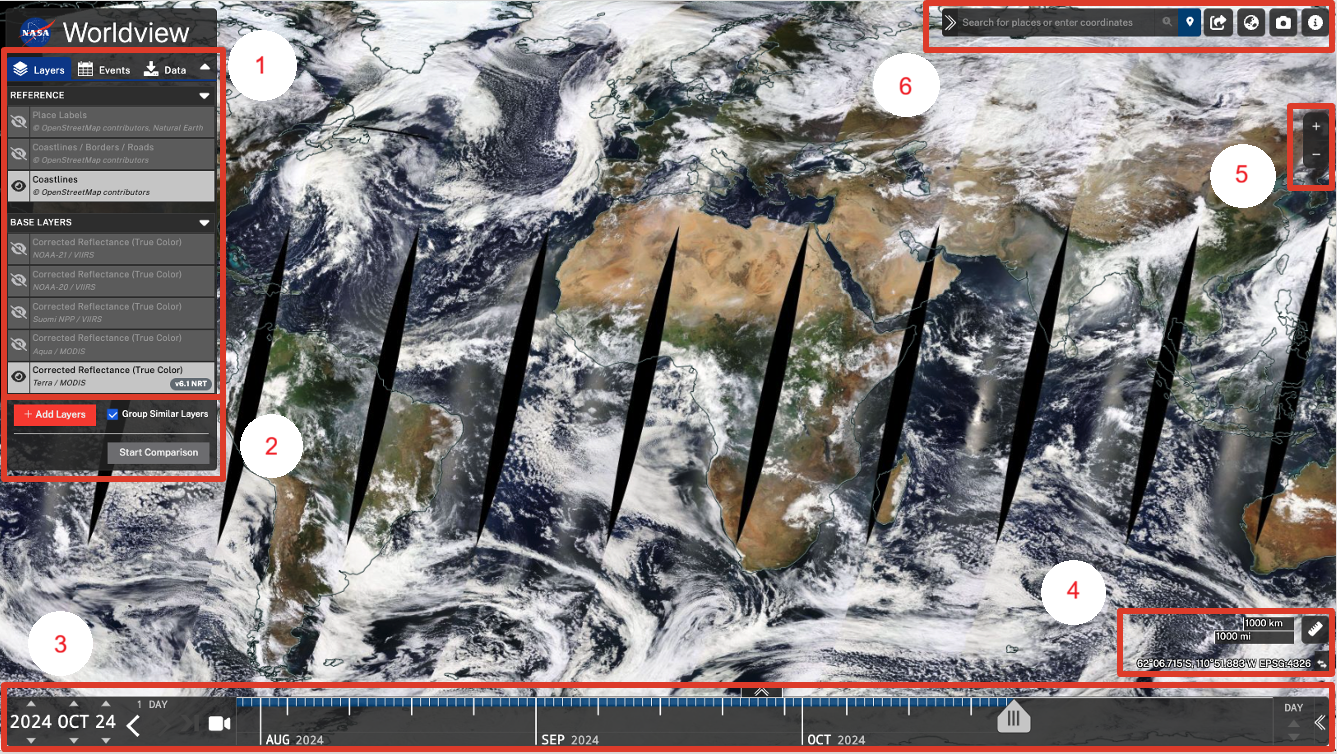
\includegraphics[width=1\textwidth,height=\textheight]{images/sensores_remotos/arset/image-671c0a86b6f36.png}
\end{center}

\subsection{Componentes de la
Interfaz}\label{componentes-de-la-interfaz}

\textbf{1. Panel de Capas, Eventos y Datos (Layers, Events and Data
Panel)} Administra las imágenes del mapa en este panel a través de tres
pestañas principales:

\begin{itemize}
\tightlist
\item
  \textbf{Pestaña Capas (Layers Tab):} Muestra todas las capas de
  imágenes que están cargadas en el mapa. Las capas base aparecen debajo
  de las superposiciones del mapa. Puedes activar y desactivar las capas
  haciendo clic en el icono del ``ojo'' a la izquierda del nombre de la
  capa. Solo se muestra la capa base activa que esté más arriba. Para
  reordenar las capas en la lista, haz clic y mantén presionado sobre
  una capa o grupo y muévelo.
\item
  \textbf{Pestaña Eventos (Events Tab):} Selecciona esta pestaña para
  ver una lista curada de eventos naturales actuales e históricos
  alrededor del mundo para cargarlos en tu mapa.
\item
  \textbf{Pestaña Descarga de Datos (Data Download Tab):} Selecciona
  esta pestaña para descargar los datos subyacentes de las capas de
  imágenes mostradas en el mapa. Serás redirigido a la herramienta
  Earthdata Search para descargar los gránulos de datos de la capa
  seleccionada, el área de interés elegida y la fecha actual.
\end{itemize}

\textbf{2. Selector de Capas (Layer Picker)}

\begin{itemize}
\tightlist
\item
  \textbf{Layer Picker:} Haz clic en el botón \emph{Add Layer} para
  explorar y buscar entre más de 1000 capas de imágenes por disciplina
  científica, categorías de riesgos y desastres, o por palabra clave.
\item
  \textbf{Iniciar Comparación (Start Comparison):} Compara imágenes de
  dos fechas diferentes, dos conjuntos de imágenes de la misma fecha, o
  incluso dos conjuntos de imágenes de fechas distintas.
\end{itemize}

\textbf{3. Gestión de la Línea de Tiempo (Timeline Management)} De
izquierda a derecha:

\begin{itemize}
\tightlist
\item
  \textbf{Selector de Fecha (Date Selector):} Cambia la fecha (y la hora
  del día si tienes capas Geoestacionarias cargadas) escribiendo en los
  campos de fecha, o haciendo clic en las flechas arriba y abajo junto a
  cada campo.
\item
  \textbf{Selector de Intervalo (Interval Selector):} Selecciona el
  intervalo de tiempo deseado y usa las flechas izquierda y derecha para
  avanzar o retroceder en el tiempo según el intervalo seleccionado. Usa
  la flecha del extremo derecho para ir a la última fecha disponible.
\item
  \textbf{Animación (Animation):} Anima las imágenes haciendo clic en el
  ícono de la cámara de video. Haz clic en el botón \emph{Play} para ver
  cómo cambian las imágenes. También puedes seleccionar un área para
  exportar como un GIF animado.
\item
  \textbf{Ajustador de Escala de Tiempo (Timescale Adjuster):} Ajusta la
  escala de tiempo a años, meses y días (además de horas y minutos si
  tienes una capa Geoestacionaria cargada).
\end{itemize}

\textbf{4. Coordenadas del Mapa y Medición (Map Coordinates and
Measurement)}

\begin{itemize}
\tightlist
\item
  \textbf{Coordenadas del Mapa:} Al pasar el cursor sobre el mapa, las
  coordenadas se muestran aquí. Haz clic en las coordenadas para cambiar
  entre formatos comunes como Grados Decimales (DD), Grados Minutos
  Decimales (DDM) y Grados Minutos Segundos (DMS).
\item
  \textbf{Medir (Measure):} Mide distancias y áreas en kilómetros (km) o
  millas (mi) y expórtalas como GeoJSON.
\end{itemize}

\textbf{5. Zoom}

\begin{itemize}
\tightlist
\item
  Usa los botones \textbf{+/-} para acercar y alejar, o usa la
  funcionalidad de zoom incorporada en tu dispositivo.
\end{itemize}

\textbf{6. Búsqueda, Compartir y más (Search, Share and more)} Opciones
del menú superior derecho, de izquierda a derecha:

\begin{itemize}
\tightlist
\item
  \textbf{Buscar por ubicación (Search by location):} Busca por nombre o
  coordenadas, lo cual coloca un marcador en el mapa. Por el contrario,
  coloca un marcador en el mapa para averiguar el nombre del lugar y sus
  coordenadas.
\item
  \textbf{Compartir URL Personalizada (Share Custom URL):} Crea un
  enlace URL personalizado de tu vista del mapa en Worldview. Acredita a
  Worldview utilizando el texto de citación proporcionado.
\item
  \textbf{Proyecciones del Mapa (Map Projections):} Cambia la proyección
  del mapa de Geográfica a Ártica o Antártica.
\item
  \textbf{Captura (Snapshot):} Toma una captura de las imágenes
  mostradas en el mapa y expórtalas como GeoTIFF, JPG con Worldfile, PNG
  con Worldfile o KMZ para llevarlas directamente a clientes SIG.
\item
  \textbf{Información (Information):} Ajusta la configuración, explora
  la aplicación a través de recorridos guiados, revisa notificaciones
  del servicio, envía comentarios y descubre más sobre el código
  abierto. También puedes acceder al modo \emph{Distraction Free}, que
  oculta la mayor parte de la aplicación para que puedas concentrarte
  solo en el mapa.
\end{itemize}

\begin{quote}
💡 \textbf{Nota:} Esta sección es una adaptación. Si deseas profundizar
más, puedes acceder al \href{https://go.nasa.gov/48kMhMc}{tutorial
original para explorar Worldview aquí}.
\end{quote}

\begin{center}\rule{0.5\linewidth}{0.5pt}\end{center}

\section{Exploración de Worldview
(Práctica)}\label{exploraciuxf3n-de-worldview-pruxe1ctica}

Ahora que has explorado algunas de las características de la
herramienta, usaremos este \href{https://go.nasa.gov/3CbFnMW}{escenario
de mapa personalizado de WorldView} para responder a las preguntas a
continuación. Puedes abrir este escenario en otra pestaña del navegador
si te resulta más fácil mientras respondes.

\subsection{Ejercicio 1: Comparación de Sensores de Órbita
Polar}\label{ejercicio-1-comparaciuxf3n-de-sensores-de-uxf3rbita-polar}

En el panel de Capas (Layers), usa el ícono del ojo para ocultar todas
las capas base; el mapa quedará en blanco mostrando solo los contornos
de los países. Luego, haz clic en cada ícono del ojo para encender y
apagar cada capa individualmente y comparar las diferencias en las
imágenes.

\textbf{Pregunta:} Al ver las imágenes MODIS de los satélites Aqua y
Terra, se observan franjas negras alrededor de los trópicos. Esta
característica no se ve al observar imágenes de VIIRS en los satélites
Suomi NPP, NOAA-20 y NOAA-21. ¿Por qué se ve esto en las imágenes MODIS,
pero no en VIIRS?

\subsection{Ejercicio 2: Satélites
Geoestacionarios}\label{ejercicio-2-satuxe9lites-geoestacionarios}

Oculta todas las capas base y asegúrate de \textbf{alejar el zoom para
poder ver tanto América del Norte como América del Sur}. Sobre las capas
base, verás dos capas de los satélites NOAA GOES Este y Oeste bajo el
encabezado `Geostationary'. Haz clic en los íconos del ojo de ambas.

En el panel de la \textbf{línea de tiempo} en la parte inferior,
\textbf{cambia la fecha a uno, dos, tres, cuatro, o cinco días antes de
la fecha actual} (\emph{Nota: Dependiendo del tamaño de tu navegador,
puede que necesites desplazarte hacia abajo para ver el panel de la
línea de tiempo}). Usa el \textbf{ícono del ojo} para alternar y
comparar las diferencias entre la capa actual y las capas base.
\textbf{Si las imágenes GOES no se muestran, intenta con otras fechas}.

\textbf{Pregunta:} Al ver las capas GOES, hay imágenes sobre América del
Norte y del Sur, y espacio negro a ambos lados de la imagen. ¿Por qué
estas imágenes se ven diferentes a las disponibles en las capas base?

\subsection{Ejercicio 3: Incendios Forestales (Modo
Comparación)}\label{ejercicio-3-incendios-forestales-modo-comparaciuxf3n}

En el siguiente \href{https://go.nasa.gov/4j3Mc4s}{escenario
personalizado de Worldview sobre Incendios}, se utiliza el ``modo de
comparación'' para mostrar diferentes capas para el mismo día (8 de
agosto de 2021).

La capa base en el \textbf{Lado `A' (Izquierda)} muestra imágenes de
color verdadero de VIIRS (en el satélite NOAA-20). La capa base en el
\textbf{Lado `B' (Derecha)} muestra imágenes de falso color de VIIRS
(satélite NOAA-20). Usa la barra deslizante central para interactuar con
el mapa y comparar.

\subsubsection{Lado A (Izquierda)}\label{lado-a-izquierda}

Además de la capa base de color verdadero, el Lado A tiene las
siguientes capas:

\begin{itemize}
\tightlist
\item
  VIIRS Incendios y Anomalías Térmicas, Día (visible)
\item
  VIIRS Incendios y Anomalías Térmicas, Noche (oculta)
\end{itemize}

Los incendios y otras anomalías térmicas, como las antorchas de gas,
muestran fuertes emisiones en la parte del Infrarrojo Medio (Mid-IR) del
espectro electromagnético. Sensores como VIIRS utilizan un algoritmo que
aprovecha esta fuerte emisión para detectar incendios activos.

En el Lado A, usa el ícono del ojo en el panel de capas para
\textbf{ocultar} las detecciones de incendios diurnos de VIIRS y
\textbf{mostrar} las detecciones de incendios nocturnos.

\textbf{Pregunta:} Dado que VIIRS es un sensor pasivo de órbita polar,
¿por qué es capaz de detectar incendios por la noche?

\subsubsection{Lado B (Derecha)}\label{lado-b-derecha}

El Lado `B' muestra las mismas capas de Incendios y Anomalías Térmicas
de VIIRS, pero con una capa base diferente. La capa base del Lado B es
una \textbf{imagen de falso color} de VIIRS. Esta combinación de falso
color incluye:

\begin{itemize}
\tightlist
\item
  Rojo: Infrarrojo de onda corta o SWIR (Banda M11)
\item
  Verde: Infrarrojo cercano o NIR (Banda I2)
\item
  Azul: Visible (Banda I1)
\end{itemize}

Usa la barra deslizante para comparar las capas base de los lados A y B.

\textbf{Pregunta:} En el Lado B, ¿por qué las áreas que se han quemado
(cicatrices de quema) aparecen de color rojo?

\subsection{Ejercicio 4: Firmas Espectrales
(Emparejamiento)}\label{ejercicio-4-firmas-espectrales-emparejamiento}

Empareja cada material con la descripción de cómo su superficie responde
a la radiación electromagnética incidente. Selecciona la opción correcta
en cada lista desplegable y haz clic en ``Comprobar Respuestas''.

\subsection{Ejercicio 5: Conceptos Fundamentales de Sensores
Remotos}\label{ejercicio-5-conceptos-fundamentales-de-sensores-remotos}

Pon a prueba tu conocimiento sobre los principios de la teledetección,
órbitas y productos de datos. Haz clic en la opción que consideres
correcta.

\textbf{1. ¿Cuáles de las siguientes afirmaciones sobre la teledetección
de la atmósfera terrestre son correctas?}

\begin{enumerate}
\def\labelenumi{\arabic{enumi}.}
\tightlist
\item
  Las nubes son altamente reflectantes para todas las longitudes de onda
  de la luz visible.
\item
  Muchos tipos de contaminación (ej. humo, polvo) absorben más en
  longitudes de onda visibles.
\item
  Los científicos que estudian la superficie terrestre deben tener en
  cuenta los efectos de las nubes, gases traza y aerosoles en la
  atmósfera al usar datos satelitales.
\item
  La atmósfera es completamente transparente a longitudes de onda
  visibles, pero opaca a la radiación infrarroja y ultravioleta.
\item
  Todos los sensores remotos de la NASA están diseñados para ``ver a
  través'' de las nubes.
\end{enumerate}

\textbf{2. Empareja cada característica deseada de los datos satelitales
con el tipo de órbita más probable para cumplirla.}

\textbf{3. Los sensores remotos ACTIVOS dependen de la luz solar que se
refleja o se vuelve a emitir desde la Tierra para realizar mediciones.}

\textbf{4. ¿Cuál es la relación general entre la resolución espacial y
la cobertura espacial (ancho de barrido) para los sensores satelitales?}

\textbf{5. Empareja el tiempo de revisita (resolución temporal) del
satélite/sensor más apropiado para los siguientes escenarios:}

\textbf{6. Las imágenes de sensores remotos por satélite siempre
muestran exactamente lo que ``ve'' el instrumento de la misma forma que
una cámara fotográfica tradicional.}

\textbf{7. ¿Cuál es el nivel más bajo de procesamiento de datos en el
que encontrarás variables geofísicas con control de calidad alineadas en
cuadrículas uniformes (grids) en el espacio y el tiempo?}

\textbf{8. ¿Cuáles de los siguientes son beneficios comunes del uso de
datos de observación de la Tierra por sensores remotos?}

\begin{enumerate}
\def\labelenumi{\arabic{enumi}.}
\tightlist
\item
  Un solo sensor puede usarse para medir toda o una gran parte de la
  Tierra.
\item
  La NASA cobra una tarifa por descargar datos para financiar mejores
  sensores.
\item
  La teledetección es la forma más directa y precisa de medir cualquier
  cantidad geofísica.
\item
  Se pueden recolectar datos incluso de lugares difíciles de alcanzar en
  el terreno.
\item
  Algunos datos están disponibles en pocas horas, permitiendo decisiones
  casi en tiempo real.
\end{enumerate}

\textbf{9. Todas las siguientes son \emph{debilidades} o retos de usar
datos de sensores remotos de la NASA, EXCEPTO:}

\textbf{10. Todos los datos y herramientas de teledetección de la NASA
se pueden buscar y acceder a través del sitio web Earthdata de la NASA
sin costo alguno.}

\chapter{Guía de Instalación y Uso: NASA Earthdata Plugin para
QGIS}\label{guuxeda-de-instalaciuxf3n-y-uso-nasa-earthdata-plugin-para-qgis}

Acceso y descarga de productos satelitales de la NASA

\hfill\break

\section{Resumen del Plugin}\label{resumen-del-plugin}

El \textbf{NASA Earthdata QGIS Plugin} es una herramienta diseñada para
buscar, visualizar y descargar productos de NASA Earthdata directamente
dentro del entorno de QGIS. Facilita el acceso al catálogo de datos de
ciencias de la Tierra de la NASA, soportando la visualización de Cloud
Optimized GeoTIFFs (COG) y la visualización de huellas espaciales
(footprints).

\subsection{Características
Principales}\label{caracteruxedsticas-principales}

\begin{itemize}
\tightlist
\item
  \textbf{Búsqueda en el Catálogo:} Explora miles de conjuntos de datos
  utilizando palabras clave, cajas delimitadoras (bounding boxes) y
  filtros temporales.
\item
  \textbf{Visualización de Footprints:} Muestra las huellas de los
  resultados de búsqueda directamente en el lienzo del mapa de QGIS.
\item
  \textbf{Soporte COG:} Transmite y visualiza archivos Cloud Optimized
  GeoTIFF directamente sin necesidad de descargarlos.
\item
  \textbf{Descarga de Datos:} Descarga gránulos para procesamiento y
  visualización local.
\item
  \textbf{Integración de Credenciales:} Autenticación fluida con las
  credenciales de NASA Earthdata Login.
\item
  \textbf{Panel de Configuración:} Configura credenciales, preferencias
  de descarga y opciones del plugin.
\item
  \textbf{Limitaciones:}

  \begin{itemize}
  \tightlist
  \item
    Los datos no están estandarizados como en GEE.
  \item
    Algunos datasets se pueden ver en QGIS (principalmente el formato
    Cloud Optimized Geotiff - COG), otros es necesario descargarlos.
  \item
    Quizás convenga buscar primero su dataset en GEE y en caso de que no
    se encuentra allí, entonces usar este plugin de los datos de la Nasa
    en QGIS.
  \end{itemize}
\end{itemize}

\begin{center}\rule{0.5\linewidth}{0.5pt}\end{center}

\section{Prerrequisitos}\label{prerrequisitos}

Antes de iniciar la instalación, asegúrate de contar con lo siguiente:

\begin{enumerate}
\def\labelenumi{\arabic{enumi}.}
\tightlist
\item
  \textbf{QGIS:} Versión 3.28 o superior.
\item
  \textbf{Cuenta de NASA Earthdata:} Es necesario registrarse (de forma
  gratuita) en
  \href{https://urs.earthdata.nasa.gov/}{urs.earthdata.nasa.gov}.
\end{enumerate}

\begin{center}\rule{0.5\linewidth}{0.5pt}\end{center}

\section{Enlaces Importantes}\label{enlaces-importantes}

\begin{itemize}
\tightlist
\item
  \textbf{Página del Plugin en QGIS:}
  \href{https://plugins.qgis.org/plugins/nasa_earthdata/}{plugins.qgis.org/plugins/nasa\_earthdata}
\item
  \textbf{Guía de instalación y GitHub:}
  \href{https://github.com/opengeos/qgis-nasa-earthdata-plugin}{github.com/opengeos/qgis-nasa-earthdata-plugin}
\item
  \textbf{Video Tutorial paso a paso:}
  \href{https://youtu.be/H78l-3nbPfk}{youtu.be/H78l-3nbPfk}
\item
  \textbf{Cuenta NASA Earthdata:}
  \href{https://urs.earthdata.nasa.gov/}{urs.earthdata.nasa.gov}
\item
  \textbf{Catálogo NASA Earthdata:}
  \href{https://www.earthdata.nasa.gov/}{www.earthdata.nasa.gov/}
\end{itemize}

\section{Instalación del Entorno}\label{instalaciuxf3n-del-entorno}

\href{https://youtu.be/H78l-3nbPfk}{Video gúia: The Easiest Way to
Access 120 Petabytes of NASA Data Inside QGIS}

Para evitar conflictos con las dependencias de Python de QGIS, se
recomienda instalar QGIS y las librerías necesarias utilizando Pixi.

\subsection{1. Instalar QGIS con PIXI}\label{instalar-qgis-con-pixi}

Ver Sección~\ref{sec-qgis-gee-pixi}.

\subsection{2. Crear un proyecto PIXI}\label{crear-un-proyecto-pixi}

Ver Sección~\ref{sec-qgis-gee-pixi}.

\subsection{3. Instalar las
Dependencias}\label{instalar-las-dependencias}

En Sección~\ref{sec-qgis-gee-pixi} se instaló un QGIS con las
dependencias para el plugin de GEE en QGIS.

\begin{itemize}
\tightlist
\item
  \textbf{Opción A:} Si usa el mismo proyecto PIXI, no debe instalar
  QGIS ni \texttt{geopandas} nuevamente. Desde la carpeta donde creó el
  proyecto PIXI (ej: \texttt{geo}), instala QGIS y los paquetes de
  Python requeridos (\texttt{earthaccess} y \texttt{geopandas}):
\end{itemize}

\begin{Shaded}
\begin{Highlighting}[]
\ExtensionTok{pixi}\NormalTok{ add earthaccess}
\end{Highlighting}
\end{Shaded}

\begin{itemize}
\tightlist
\item
  \textbf{Opción B:} Si usa un proyecto nuevo de PIXI, debe instalar
  todos los requerimientos: Desde la carpeta donde creó el proyecto
  nuevo de PIXI (ej: \texttt{geo\_nuevo}), instala QGIS y los paquetes
  de Python requeridos (\texttt{earthaccess} y \texttt{geopandas}):
\end{itemize}

\begin{Shaded}
\begin{Highlighting}[]
\ExtensionTok{pixi}\NormalTok{ add qgis earthaccess geopandas}
\end{Highlighting}
\end{Shaded}

\section{Instalación del Plugin en
QGIS}\label{instalaciuxf3n-del-plugin-en-qgis}

Se recomienda instalar el plugin a través del Administrador de
Complementos de QGIS:

\begin{enumerate}
\def\labelenumi{\arabic{enumi}.}
\tightlist
\item
  Abre QGIS utilizando tu entorno PIXI. Desde el PowerShell y estando
  ubicado en la carpeta del proyecto de PIXI:
\end{enumerate}

\begin{Shaded}
\begin{Highlighting}[]
\ExtensionTok{pixi}\NormalTok{ run qgis}
\end{Highlighting}
\end{Shaded}

\begin{enumerate}
\def\labelenumi{\arabic{enumi}.}
\setcounter{enumi}{1}
\tightlist
\item
  Ve a \textbf{Complementos} \textgreater{} \textbf{Administrar e
  instalar complementos\ldots{}}
\item
  Ve a la pestaña \textbf{Configuración}.
\item
  Haz clic en \textbf{Añadir\ldots{}} en la sección ``Repositorios de
  complementos''.
\item
  Asigna un nombre al repositorio, por ejemplo: \texttt{OpenGeos}.
\item
  Ingresa la URL del repositorio:
  \texttt{https://qgis.gishub.org/plugins.xml}
\item
  Haz clic en \textbf{Aceptar}.
\item
  Ve a la pestaña \textbf{Todos}, busca \textbf{``NASA Earthdata''}.
\item
  Selecciona el plugin en la lista y haz clic en \textbf{Instalar
  complemento}.
\end{enumerate}

\begin{center}\rule{0.5\linewidth}{0.5pt}\end{center}

\section{Guía de Uso}\label{guuxeda-de-uso}

\subsection{Autenticación}\label{autenticaciuxf3n}

Antes de usar el plugin, debes configurar tus credenciales de NASA
Earthdata:

\begin{enumerate}
\def\labelenumi{\arabic{enumi}.}
\tightlist
\item
  Haz clic en \textbf{NASA Earthdata} \textgreater{} \textbf{Settings}
  en el menú superior.
\item
  Ingresa tu nombre de usuario y contraseña de Earthdata.
\item
  Haz clic en \textbf{Test Credentials} para verificar.
\item
  Haz clic en \textbf{Save Settings}.
\end{enumerate}

\begin{quote}
\textbf{Nota 1:} Alternativamente, puedes configurar las credenciales
mediante variables de entorno (\texttt{EARTHDATA\_USERNAME} y
\texttt{EARTHDATA\_PASSWORD}) o usando un archivo \texttt{.netrc}
asociado a \texttt{urs.earthdata.nasa.gov}. \textbf{Nota 2:} La primera
vez que se salva la configuracion se crea el archivo \texttt{.netrc}
\textbf{Nota 3:} Si el nombre del archivo \texttt{.netrc} se torna de
color \texttt{verde} es una buena señal que la autenticación está
lista/completa.
\end{quote}

\subsection{Actualizar el Plugin}\label{actualizar-el-plugin}

Menú \texttt{NASA\ Earthdata} -\textgreater{}
\texttt{Check\ for\ Updates}. Luego clic en el botón
\texttt{Check\ for\ Updates}. Si aplica, clic en
\texttt{Download\ and\ Install\ Update}. Después de instalar debe salir
un mensaje: \texttt{Status:\ You\ are\ running\ the\ last\ version!}

Después de instalar debe \textbf{cerrar y abrir} nuevamente QGIS:
\texttt{pixi\ run\ qgis}

\subsection{Agregar un Basemap}\label{agregar-un-basemap}

Ejecute el archivo \texttt{./docs/qgis\_basemaps.py} en la consola de
Python de QGIS.

\begin{figure}[H]

{\centering 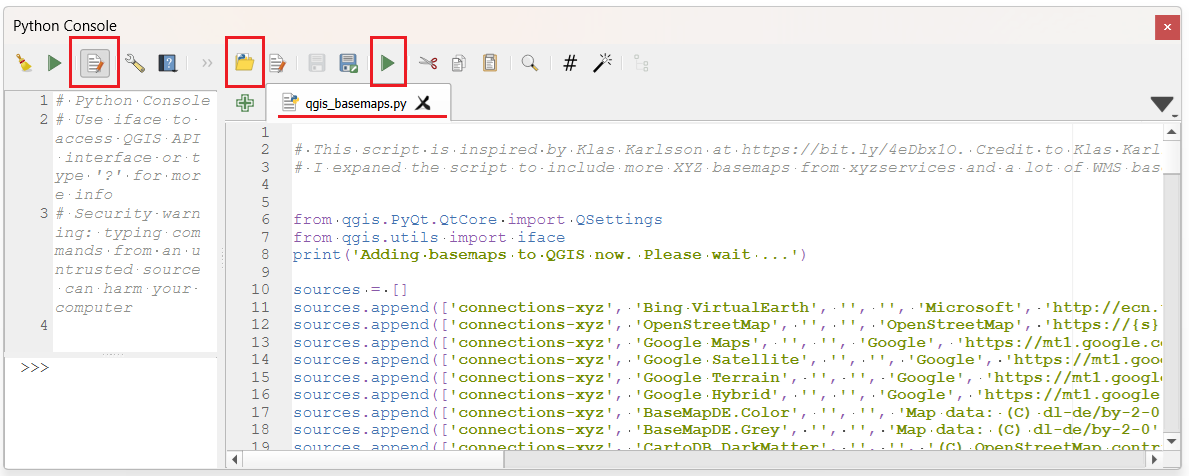
\includegraphics[width=1\textwidth,height=\textheight]{images/qgis/qgis_basemaps_python.png}

}

\caption{Archivo qgis\_basemaps.py en la consola de Python de QGIS}

\end{figure}%

Luego en el \texttt{Browser\ Panel} (Panel de Búsqueda) cargue un mapa
base en la sección \texttt{XYZ\ Tiles}:

\begin{figure}[H]

{\centering 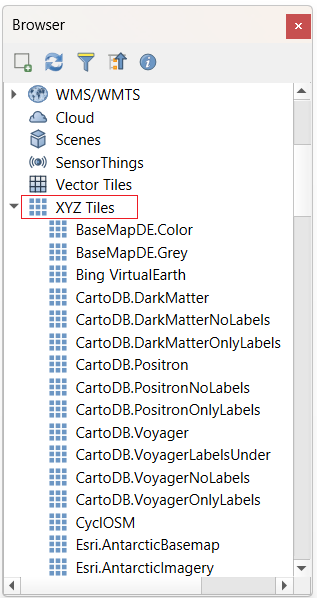
\includegraphics[width=0.3\textwidth,height=\textheight]{images/qgis/basemaps_qgis.png}

}

\caption{Mapas base en la sección \texttt{XYZ\ Tiles} en el
\texttt{Browser\ Panel} de QGIS}

\end{figure}%

\subsection{Búsqueda de Datos}\label{buxfasqueda-de-datos}

\begin{enumerate}
\def\labelenumi{\arabic{enumi}.}
\tightlist
\item
  Haz clic en el botón \textbf{NASA Earthdata Search} en la barra de
  herramientas.
\item
  Filtra los conjuntos de datos por palabra clave (opcional). Ejemplo
  \texttt{HLS} para los datos armonizados de Landsat y Sentinel.
\item
  Selecciona un conjunto de datos del menú desplegable (pueden aparecer
  duplicados).
\item
  Establece el \emph{Bounding box} (caja delimitadora) o usa la
  extensión actual del mapa. Una vez haga acercamiento (\emph{zoom}) a
  la zona de interés de clic en \texttt{Use\ Map\ Extent}
\item
  Define el rango de fechas.
\item
  Puede habilitar \texttt{Advanced\ Options} para filtrar por:

  \begin{itemize}
  \tightlist
  \item
    Cobertura de nubes.
  \item
    Captura de día o de noche.
  \item
    Proveedor
  \item
    Versión
  \item
    Granule ID
  \item
    Número de Órbita
  \end{itemize}
\item
  Haz clic en \textbf{Search}.
\end{enumerate}

\subsection{Visualización}\label{visualizaciuxf3n}

\begin{itemize}
\tightlist
\item
  \textbf{Footprints:} Los resultados de la búsqueda se muestran
  automáticamente como huellas espaciales en el mapa.
\item
  \textbf{Capas COG:} Selecciona los resultados deseados y haz clic en
  \textbf{Display COG} para transmitir la imagen sin descargarla.
\item
  \textbf{Datos Descargados:} Tras la descarga, puedes añadir los
  archivos ráster directamente al mapa.
\end{itemize}

\begin{enumerate}
\def\labelenumi{\arabic{enumi}.}
\setcounter{enumi}{7}
\tightlist
\item
  El plugin busca todos los \texttt{footprints} del área de interés.
  Puedes dar clic en la herramienta \texttt{Identify\ Features}
  (\texttt{Ctrl\ +\ Shift\ +\ I}).
\item
  En \texttt{Search\ Results} (caja de resultados) verás la lista de
  datos disponibles. Seleccione el deseado de la lista.
\item
  Clic \texttt{Zoom\ to\ Footprints} y remueva cualquier selección
  realizada en los \texttt{footprints}
  (\texttt{Deselect\ features\ from\ all\ layers} o
  \texttt{Ctrl\ +\ Alt\ +\ A}).
\item
  Clic en el botón \texttt{Display\ COG} (Mostrar COG). Note que hay una
  conexión COG por banda, así que debe seleccionar la banda deseada la
  lista \texttt{COG\ File}.
\end{enumerate}

Esto no es tan rápido como GEE, porque usa COG para cargar bajo demanda,
en cambio GEE usa \texttt{XYZ\ tile} (más rápido y maneja área más
grande). Proceda al descargar si está satisfecho con el archivo y la
banda seleccionada.

\subsection{Descarga de Datos}\label{descarga-de-datos-1}

\begin{itemize}
\tightlist
\item
  Selecciona los gránulos que deseas descargar desde la tabla de
  resultados.
\end{itemize}

\begin{enumerate}
\def\labelenumi{\arabic{enumi}.}
\setcounter{enumi}{11}
\tightlist
\item
  Clic en \texttt{Download} (Descargar).
\item
  Seleccione \texttt{Yes} (si). Seleccione la carpeta destino.
\item
  Espera a que se complete la descarga e intégralos a tu proyecto en
  QGIS.
\end{enumerate}

\begin{quote}
\textbf{Nota 4}: Descargará \textbf{todas las bandas} del archivo
seleccionado a la carpeta seleccionada. \textbf{Nota 5}: Si no
selecciona nada de la lista (punto 8), el sistema descargará todos los
archivos listados en la ventana \texttt{Search\ Results}.
\end{quote}

\begin{enumerate}
\def\labelenumi{\arabic{enumi}.}
\setcounter{enumi}{14}
\tightlist
\item
  Presione el botón \texttt{Reset} (Resetear) para volver a empezar
\end{enumerate}

\begin{center}\rule{0.5\linewidth}{0.5pt}\end{center}

\section{Descargar GEDI}\label{descargar-gedi}

GEDI (Global Ecosystem Dynamics Investigation): Instalado en la Estación
Espacial Internacional (ISS), registra datos entre las latitudes 51.6° N
y 51.6° S, abarcando la totalidad del territorio colombiano. Ofrece
productos desde el nivel L1B (formas de onda geolocalizadas) hasta los
niveles L4A y L4B (estimaciones de biomasa aérea e índices de estructura
forestal).

\begin{figure}[H]

{\centering 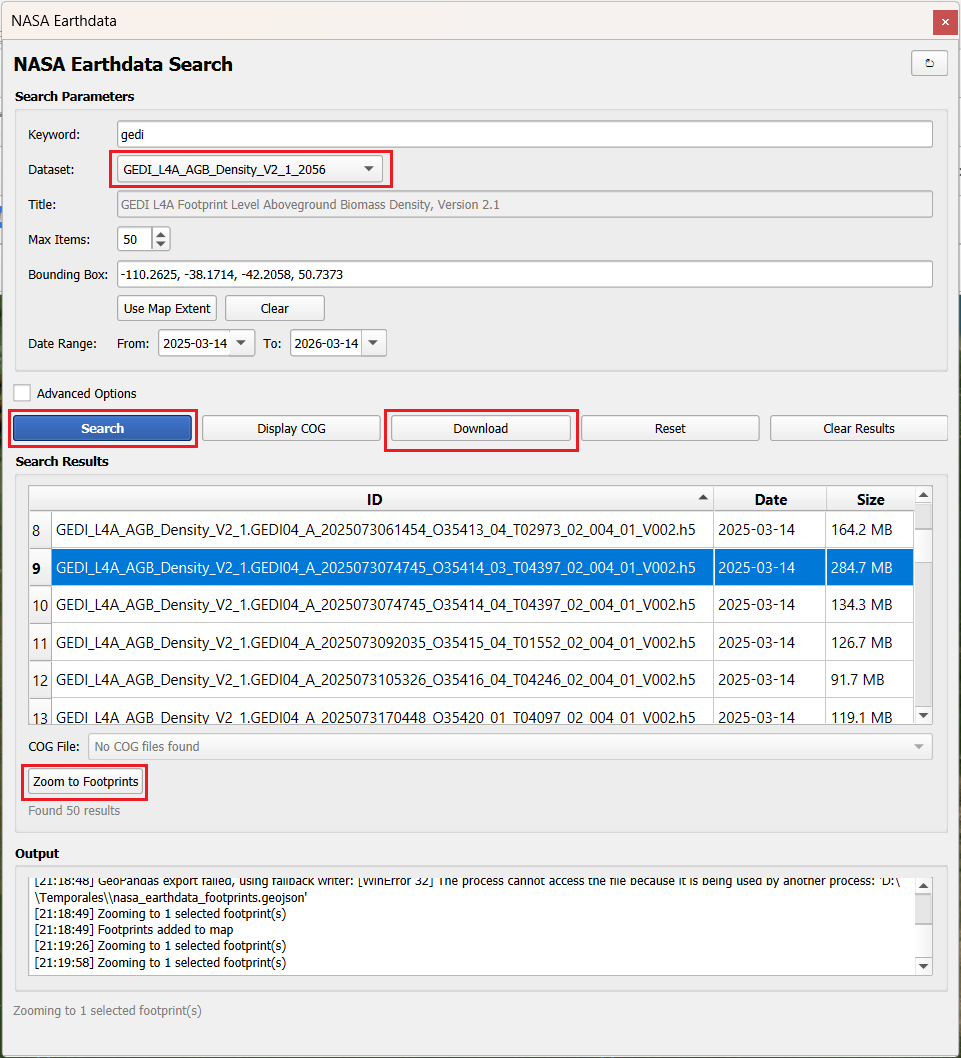
\includegraphics[width=1\textwidth,height=\textheight]{images/qgis/gedi_colombia_2025.png}

}

\caption{Decarga de datos LiDAR del dataset GEDI}

\end{figure}%

\section{Conjuntos de Datos
Soportados}\label{conjuntos-de-datos-soportados}

El plugin proporciona acceso a miles de conjuntos de datos de la NASA,
incluyendo:

\begin{itemize}
\tightlist
\item
  \textbf{GEDI:} Investigación de la dinámica de los ecosistemas
  globales (estructura forestal, biomasa).
\item
  \textbf{MODIS:} Espectrorradiómetro de imágenes de resolución
  moderada.
\item
  \textbf{Landsat:} Imágenes de Landsat 8 y 9.
\item
  \textbf{VIIRS:} Conjunto de radiómetros de imágenes infrarrojas
  visibles.
\item
  \textbf{SMAP:} Humedad del suelo activa pasiva.
\item
  \textbf{ICESat-2:} Satélite de elevación de hielo, nubes y tierra.
\item
  \textbf{OPERA:} Productos observacionales para usuarios finales a
  partir de análisis de teledetección.
\item
  \emph{Y muchos más\ldots{}}
\end{itemize}

\begin{center}\rule{0.5\linewidth}{0.5pt}\end{center}

\section{Solución de Problemas
(Troubleshooting)}\label{soluciuxf3n-de-problemas-troubleshooting}

Si el plugin no se carga debido a paquetes faltantes, asegúrate de
instalar las dependencias en el entorno correcto:

\textbf{Usando pip en tu entorno activo:}

\begin{Shaded}
\begin{Highlighting}[]
\ExtensionTok{pip}\NormalTok{ install earthaccess geopandas}
\end{Highlighting}
\end{Shaded}

\textbf{O usando el entorno de Python específico de QGIS (ej. en
Linux):}

\begin{Shaded}
\begin{Highlighting}[]
\ExtensionTok{\textasciitilde{}/.local/share/QGIS/QGIS3/profiles/default/python/plugins/nasa\_earthdata/}
\ExtensionTok{python3} \AttributeTok{{-}m}\NormalTok{ pip install earthaccess geopandas}
\end{Highlighting}
\end{Shaded}

\begin{center}\rule{0.5\linewidth}{0.5pt}\end{center}

\part{Presentaciones}

\chapter{Temas por Charlar}\label{temas-por-charlar}

Asunto: varios

\hfill\break

\section{Enfoque Open Science}\label{enfoque-open-science}

\begin{itemize}
\tightlist
\item
  Material presentado por profesor

  \begin{itemize}
  \tightlist
  \item
    Diapositivas
  \item
    Código
  \item
    Teoría
  \item
    Archivos de configuración
  \end{itemize}
\item
  Material de los estudiantes
\item
  HTML, PDF
\item
  GitHub
\end{itemize}

🚫 Evitar guardar su trabajo en los discos duros.

\begin{center}\rule{0.5\linewidth}{0.5pt}\end{center}

\section{Clase de Hoy: Instalación y uso básico de
Herramientas}\label{clase-de-hoy-instalaciuxf3n-y-uso-buxe1sico-de-herramientas}

\begin{itemize}
\tightlist
\item
  \begin{enumerate}
  \def\labelenumi{\arabic{enumi}.}
  \tightlist
  \item
    Contenedores Docker
  \end{enumerate}
\item
  \begin{enumerate}
  \def\labelenumi{\arabic{enumi}.}
  \setcounter{enumi}{1}
  \tightlist
  \item
    VSCode
  \end{enumerate}
\item
  \begin{enumerate}
  \def\labelenumi{\arabic{enumi}.}
  \setcounter{enumi}{2}
  \tightlist
  \item
    Git
  \end{enumerate}
\item
  \begin{enumerate}
  \def\labelenumi{\arabic{enumi}.}
  \setcounter{enumi}{3}
  \tightlist
  \item
    Docker Desktop
  \end{enumerate}
\item
  \begin{enumerate}
  \def\labelenumi{\arabic{enumi}.}
  \setcounter{enumi}{4}
  \tightlist
  \item
    Jupyter Lab
  \end{enumerate}
\item
  \begin{enumerate}
  \def\labelenumi{\arabic{enumi}.}
  \setcounter{enumi}{5}
  \tightlist
  \item
    VSCode
  \end{enumerate}
\item
  \begin{enumerate}
  \def\labelenumi{\arabic{enumi}.}
  \setcounter{enumi}{6}
  \tightlist
  \item
    Archivos Quarto: HTML \& PDF
  \end{enumerate}
\item
  \begin{enumerate}
  \def\labelenumi{\arabic{enumi}.}
  \setcounter{enumi}{7}
  \tightlist
  \item
    QGIS 1 (instalación)
  \end{enumerate}
\item
  \begin{enumerate}
  \def\labelenumi{\arabic{enumi}.}
  \setcounter{enumi}{8}
  \tightlist
  \item
    QGIS 2 (instalación)
  \end{enumerate}
\item
  \begin{enumerate}
  \def\labelenumi{\arabic{enumi}.}
  \setcounter{enumi}{9}
  \tightlist
  \item
    Chequeo ArcGIS Pro
  \end{enumerate}
\end{itemize}

\begin{center}\rule{0.5\linewidth}{0.5pt}\end{center}

\section{Contenido - Syllabus (Semana
2)}\label{contenido---syllabus-semana-2}

Parte 1: \textbf{Fundamentos }

Teoría:

\begin{itemize}
\tightlist
\item
  \begin{enumerate}
  \def\labelenumi{\arabic{enumi}.}
  \tightlist
  \item
    Avances y Tendencias de la Geomática
  \end{enumerate}
\end{itemize}

Ejercicios:

\begin{itemize}
\tightlist
\item
  Acceder a Geoportales y Bases de Datos
\end{itemize}

Trabajo Independiente:

\begin{itemize}
\tightlist
\item
  Lectura: Capítulo 1: Geomatics.(Gomarasca, 2009)
\end{itemize}

\begin{center}\rule{0.5\linewidth}{0.5pt}\end{center}

\section{Contenido - Syllabus (Semana 3 y
4)}\label{contenido---syllabus-semana-3-y-4}

Parte 1: \textbf{Fundamentos }

Teoría:

\begin{itemize}
\item
  \begin{enumerate}
  \def\labelenumi{\arabic{enumi}.}
  \setcounter{enumi}{1}
  \tightlist
  \item
    Fundamentos Geodésicos y Cartográficos
  \end{enumerate}

  \begin{itemize}
  \tightlist
  \item
    Elipsoide, geoide, datum, sistemas de coordenadas, escala, tipos de
    mapas, exactitud y precisión
  \end{itemize}
\end{itemize}

Ejercicios:

\begin{itemize}
\tightlist
\item
  Establecer los diferentes orígenes para Colombia y origen único
  nacional
\item
  Determinar escala de una fotografía aérea.
\end{itemize}

\begin{center}\rule{0.5\linewidth}{0.5pt}\end{center}

\section{Contenido - Syllabus (Semana 3 y
4)}\label{contenido---syllabus-semana-3-y-4-1}

Parte 1: \textbf{Fundamentos }

Trabajo Independiente:

\begin{itemize}
\tightlist
\item
  Exploración portales web de proyecciones cartográficas.

  \begin{itemize}
  \tightlist
  \item
    Map-Project (Jung, 2023).
  \item
    The True Size (Talmage \& Maneice, 2023)
  \end{itemize}
\item
  Lectura:

  \begin{itemize}
  \tightlist
  \item
    Escala (Demmattê et al., 2002; João, 2002; Poggio, Gimona, \&
    Brewer, 2013)
  \item
    Sistemas de Referencia (Islas \& Angelo, 2000)
  \item
    Cartografía. (Anthamatten, 2020)
  \end{itemize}
\end{itemize}

\begin{center}\rule{0.5\linewidth}{0.5pt}\end{center}

\section{\texorpdfstring{Contenido - Syllabus (Semana 5 y 6:
\textbf{SIG})}{Contenido - Syllabus (Semana 5 y 6: SIG)}}\label{contenido---syllabus-semana-5-y-6-sig}

Parte 2: \textbf{Estructuras de Datos Espaciales}

Teoría:

\begin{itemize}
\tightlist
\item
  \begin{enumerate}
  \def\labelenumi{\arabic{enumi}.}
  \setcounter{enumi}{2}
  \tightlist
  \item
    Estructura de los datos e información espacial
  \end{enumerate}
\item
  \begin{enumerate}
  \def\labelenumi{\arabic{enumi}.}
  \setcounter{enumi}{3}
  \tightlist
  \item
    Modelo de datos Vector
  \end{enumerate}
\item
  \begin{enumerate}
  \def\labelenumi{\arabic{enumi}.}
  \setcounter{enumi}{4}
  \tightlist
  \item
    Modelo de datos Raster
  \end{enumerate}
\item
  \begin{enumerate}
  \def\labelenumi{\arabic{enumi}.}
  \setcounter{enumi}{5}
  \tightlist
  \item
    Operaciones de los modelos de datos
  \end{enumerate}
\end{itemize}

\begin{center}\rule{0.5\linewidth}{0.5pt}\end{center}

\section{\texorpdfstring{Contenido - Syllabus (Semana 5 y 6:
\textbf{SIG})}{Contenido - Syllabus (Semana 5 y 6: SIG)}}\label{contenido---syllabus-semana-5-y-6-sig-1}

Parte 2: \textbf{Estructuras de Datos Espaciales}

Ejercicios:

\begin{itemize}
\tightlist
\item
  Búsqueda y descarga de modelos de datos (Vector y Raster).
\item
  Captura de información (GDB o GeoPackage).
\end{itemize}

Trabajo Independiente:

\begin{itemize}
\tightlist
\item
  Captura de información de una zona de interés.
\item
  Presentar propuesta de \textbf{trabajo final}
\item
  Libros Guía SIG (Longley et al., 2011; Shellito, 2020; Wise, 2014)
\end{itemize}

\begin{center}\rule{0.5\linewidth}{0.5pt}\end{center}

\section{\texorpdfstring{Contenido - Syllabus (Semana 7 a 9:
\textbf{Sensores
Remotos})}{Contenido - Syllabus (Semana 7 a 9: Sensores Remotos)}}\label{contenido---syllabus-semana-7-a-9-sensores-remotos}

Parte 2: \textbf{Estructuras de Datos Espaciales}

Teoría:

\begin{itemize}
\tightlist
\item
  \begin{enumerate}
  \def\labelenumi{\arabic{enumi}.}
  \setcounter{enumi}{6}
  \tightlist
  \item
    ¿Qué es percepción remota?.
  \end{enumerate}
\item
  \begin{enumerate}
  \def\labelenumi{\arabic{enumi}.}
  \setcounter{enumi}{7}
  \tightlist
  \item
    Componentes.
  \end{enumerate}
\item
  \begin{enumerate}
  \def\labelenumi{\arabic{enumi}.}
  \setcounter{enumi}{8}
  \tightlist
  \item
    Ventajas y limitaciones.
  \end{enumerate}
\item
  \begin{enumerate}
  \def\labelenumi{\arabic{enumi}.}
  \setcounter{enumi}{9}
  \tightlist
  \item
    Características de las imágenes.
  \end{enumerate}
\item
  \begin{enumerate}
  \def\labelenumi{\arabic{enumi}.}
  \setcounter{enumi}{10}
  \tightlist
  \item
    Fases del proceso de interpretación.
  \end{enumerate}
\item
  \begin{enumerate}
  \def\labelenumi{\arabic{enumi}.}
  \setcounter{enumi}{11}
  \tightlist
  \item
    Correcciones.
  \end{enumerate}
\item
  \begin{enumerate}
  \def\labelenumi{\arabic{enumi}.}
  \setcounter{enumi}{12}
  \tightlist
  \item
    Nivel de referencia.
  \end{enumerate}
\item
  \begin{enumerate}
  \def\labelenumi{\arabic{enumi}.}
  \setcounter{enumi}{13}
  \tightlist
  \item
    Reglas y métodos de interpretación.
  \end{enumerate}
\item
  \begin{enumerate}
  \def\labelenumi{\arabic{enumi}.}
  \setcounter{enumi}{14}
  \tightlist
  \item
    ¿Cómo se identifican los objetos?
  \end{enumerate}
\end{itemize}

\begin{center}\rule{0.5\linewidth}{0.5pt}\end{center}

\section{\texorpdfstring{Contenido - Syllabus (Semana 7 a 9:
\textbf{Sensores
Remotos})}{Contenido - Syllabus (Semana 7 a 9: Sensores Remotos)}}\label{contenido---syllabus-semana-7-a-9-sensores-remotos-1}

Parte 2: \textbf{Estructuras de Datos Espaciales}

Ejercicios:

\begin{itemize}
\tightlist
\item
  Revisión de Metadatos de productos de sensores remotos
\item
  Introducción a Google Earth Engine (GEE)
\item
  Revisión de Catalogo de datos de GEE
\item
  Composición de productos de sensores remotos
\item
  Cálculo de índices de productos de sensores remotos
\item
  Selección, recorte y descarga de imágenes de GEE
\item
  Análisis de datos Lidar
\end{itemize}

\begin{center}\rule{0.5\linewidth}{0.5pt}\end{center}

\section{\texorpdfstring{Contenido - Syllabus (Semana 7 a 9:
\textbf{Sensores
Remotos})}{Contenido - Syllabus (Semana 7 a 9: Sensores Remotos)}}\label{contenido---syllabus-semana-7-a-9-sensores-remotos-2}

Parte 2: \textbf{Estructuras de Datos Espaciales}

Trabajo independiente:

\begin{itemize}
\tightlist
\item
  Exploración: QGIS y SNAP
\item
  Libros Sensores Remotos

  \begin{itemize}
  \tightlist
  \item
    Chuvieco, 2020;
  \item
    De Grandi \& De Grandi, 2021;
  \item
    Dong \& Chen, 2018;
  \item
    Campbell et al., 2022;
  \item
    Melo \& Camacho, 2005
  \end{itemize}
\end{itemize}

\begin{center}\rule{0.5\linewidth}{0.5pt}\end{center}

\section{\texorpdfstring{Contenido - Syllabus (Semana 10:
\textbf{Navegación
Satelital})}{Contenido - Syllabus (Semana 10: Navegación Satelital)}}\label{contenido---syllabus-semana-10-navegaciuxf3n-satelital}

Parte 2: \textbf{Estructuras de Datos Espaciales}

Teoría:

\begin{itemize}
\tightlist
\item
  \begin{enumerate}
  \def\labelenumi{\arabic{enumi}.}
  \setcounter{enumi}{15}
  \tightlist
  \item
    ¿Qué es un sistema de navegación satelital?.
  \end{enumerate}
\item
  \begin{enumerate}
  \def\labelenumi{\arabic{enumi}.}
  \setcounter{enumi}{16}
  \tightlist
  \item
    Tipos de sistemas de navegación satelital.
  \end{enumerate}
\item
  \begin{enumerate}
  \def\labelenumi{\arabic{enumi}.}
  \setcounter{enumi}{17}
  \tightlist
  \item
    Tipos de levantamientos de información.
  \end{enumerate}
\item
  \begin{enumerate}
  \def\labelenumi{\arabic{enumi}.}
  \setcounter{enumi}{18}
  \tightlist
  \item
    Fuentes de error.
  \end{enumerate}
\end{itemize}

\begin{center}\rule{0.5\linewidth}{0.5pt}\end{center}

\section{\texorpdfstring{Contenido - Syllabus (Semana 10:
\textbf{Navegación
Satelital})}{Contenido - Syllabus (Semana 10: Navegación Satelital)}}\label{contenido---syllabus-semana-10-navegaciuxf3n-satelital-1}

Parte 2: \textbf{Estructuras de Datos Espaciales}

Ejercicios:

\begin{itemize}
\tightlist
\item
  Creación de formularios para captura de información de campo con
  sistemas de navegación satelital.
\end{itemize}

Trabajo independiente:

\begin{itemize}
\tightlist
\item
  Crear un formulario (¿?)
\item
  Libros sistemas de navegación:

  \begin{itemize}
  \tightlist
  \item
    Borre et al., 2022;
  \item
    NovAtel , 2015;
  \item
    Ogaja, 2022
  \end{itemize}
\end{itemize}

\begin{center}\rule{0.5\linewidth}{0.5pt}\end{center}

\section{\texorpdfstring{Contenido - Syllabus (Semana 11:
\textbf{Asesoría})}{Contenido - Syllabus (Semana 11: Asesoría)}}\label{contenido---syllabus-semana-11-asesoruxeda}

Parte 2: \textbf{Estructuras de Datos Espaciales}

Teoría: - \ldots{}

Ejercicios: - \ldots{}

\begin{center}\rule{0.5\linewidth}{0.5pt}\end{center}

\section{\texorpdfstring{Contenido - Syllabus (Semana 12 y 13:
\textbf{MDE})}{Contenido - Syllabus (Semana 12 y 13: MDE)}}\label{contenido---syllabus-semana-12-y-13-mde}

Parte 2: \textbf{Estructuras de Datos Espaciales}

Teoría:

\begin{itemize}
\tightlist
\item
  \begin{enumerate}
  \def\labelenumi{\arabic{enumi}.}
  \setcounter{enumi}{19}
  \tightlist
  \item
    ¿Qué es un Modelo Digital de Elevación (MDE)?.
  \end{enumerate}
\item
  \begin{enumerate}
  \def\labelenumi{\arabic{enumi}.}
  \setcounter{enumi}{20}
  \tightlist
  \item
    Creación.
  \end{enumerate}
\item
  \begin{enumerate}
  \def\labelenumi{\arabic{enumi}.}
  \setcounter{enumi}{21}
  \tightlist
  \item
    Parámetros derivados.
  \end{enumerate}
\item
  \begin{enumerate}
  \def\labelenumi{\arabic{enumi}.}
  \setcounter{enumi}{22}
  \tightlist
  \item
    Aplicaciones.
  \end{enumerate}
\end{itemize}

\begin{center}\rule{0.5\linewidth}{0.5pt}\end{center}

\section{\texorpdfstring{Contenido - Syllabus (Semana 12 y 13:
\textbf{MDE})}{Contenido - Syllabus (Semana 12 y 13: MDE)}}\label{contenido---syllabus-semana-12-y-13-mde-1}

Parte 2: \textbf{Estructuras de Datos Espaciales}

Ejercicios prácticos:

\begin{itemize}
\tightlist
\item
  Creación.
\item
  Comparación de MDE (diferentes resoluciones).
\item
  Derivar parámetros.
\item
  Aplicaciones de los MDE.
\end{itemize}

Trabajo independiente:

\begin{itemize}
\tightlist
\item
  Lectura: Definiciones y conceptos de MDE. (Florinsky, 2012; Guth et
  al., 2021).
\end{itemize}

\begin{center}\rule{0.5\linewidth}{0.5pt}\end{center}

\section{\texorpdfstring{Contenido - Syllabus (Semana 14:
\textbf{Cartografía
Digital})}{Contenido - Syllabus (Semana 14: Cartografía Digital)}}\label{contenido---syllabus-semana-14-cartografuxeda-digital}

Parte 3: \textbf{Presentación de la Información Espacial}

Teoría:

\begin{itemize}
\tightlist
\item
  \begin{enumerate}
  \def\labelenumi{\arabic{enumi}.}
  \setcounter{enumi}{23}
  \tightlist
  \item
    Contexto espacial.
  \end{enumerate}
\item
  \begin{enumerate}
  \def\labelenumi{\arabic{enumi}.}
  \setcounter{enumi}{24}
  \tightlist
  \item
    Elementos de la cartografía.
  \end{enumerate}
\item
  \begin{enumerate}
  \def\labelenumi{\arabic{enumi}.}
  \setcounter{enumi}{25}
  \tightlist
  \item
    Fuentes de entrada.
  \end{enumerate}
\item
  \begin{enumerate}
  \def\labelenumi{\arabic{enumi}.}
  \setcounter{enumi}{26}
  \tightlist
  \item
    Edición, estructuración y procesamiento.
  \end{enumerate}
\item
  \begin{enumerate}
  \def\labelenumi{\arabic{enumi}.}
  \setcounter{enumi}{27}
  \tightlist
  \item
    Modelos del catálogo de datos.
  \end{enumerate}
\item
  \begin{enumerate}
  \def\labelenumi{\arabic{enumi}.}
  \setcounter{enumi}{28}
  \tightlist
  \item
    Diseño de la cartografía Básica
  \end{enumerate}
\item
  \begin{enumerate}
  \def\labelenumi{\arabic{enumi}.}
  \setcounter{enumi}{29}
  \tightlist
  \item
    Diseño de la cartografía Temática
  \end{enumerate}
\item
  \begin{enumerate}
  \def\labelenumi{\arabic{enumi}.}
  \setcounter{enumi}{30}
  \tightlist
  \item
    Generalización
  \end{enumerate}
\item
  \begin{enumerate}
  \def\labelenumi{\arabic{enumi}.}
  \setcounter{enumi}{31}
  \tightlist
  \item
    Metadatos - definición.
  \end{enumerate}
\item
  \begin{enumerate}
  \def\labelenumi{\arabic{enumi}.}
  \setcounter{enumi}{32}
  \tightlist
  \item
    Metadatos - estructuración.
  \end{enumerate}
\end{itemize}

\begin{center}\rule{0.5\linewidth}{0.5pt}\end{center}

\section{\texorpdfstring{Contenido - Syllabus (Semana 14:
\textbf{Cartografía
Digital})}{Contenido - Syllabus (Semana 14: Cartografía Digital)}}\label{contenido---syllabus-semana-14-cartografuxeda-digital-1}

Parte 3: \textbf{Presentación de la Información Espacial}

Ejercicios prácticos:

\begin{itemize}
\tightlist
\item
  Estructural un proyecto de cartografía digital
\end{itemize}

Trabajo independiente:

\begin{itemize}
\tightlist
\item
  Lectura: Cartografía digital

  \begin{itemize}
  \tightlist
  \item
    Kraak \& Ormeling, 2021;
  \item
    Parker \& Toms, 2022;
  \item
    Peterson, 2023;
  \item
    Slocum et al., 2022
  \end{itemize}
\end{itemize}

\begin{center}\rule{0.5\linewidth}{0.5pt}\end{center}

\section{\texorpdfstring{Contenido - Syllabus (Semana 15 y 16:
\textbf{Proyecto
Final})}{Contenido - Syllabus (Semana 15 y 16: Proyecto Final)}}\label{contenido---syllabus-semana-15-y-16-proyecto-final}

Parte 4: \textbf{Aplicaciones de la Geomática}

Tópicos:

\begin{itemize}
\tightlist
\item
  \begin{enumerate}
  \def\labelenumi{\arabic{enumi}.}
  \setcounter{enumi}{33}
  \tightlist
  \item
    ¿Por qué socializar los resultados de una investigación?
  \end{enumerate}
\end{itemize}

Ejercicios prácticos:

\begin{itemize}
\tightlist
\item
  Sustentación.
\end{itemize}

\begin{center}\rule{0.5\linewidth}{0.5pt}\end{center}

\section{\texorpdfstring{Contenido - Syllabus
(\textbf{Evaluación})}{Contenido - Syllabus (Evaluación)}}\label{contenido---syllabus-evaluaciuxf3n}

\begin{itemize}
\tightlist
\item
  Talleres teórico-prácticos (60\%)
\item
  Trabajo final (40\%)
\end{itemize}

\section{\texorpdfstring{Contenido - Syllabus
(\textbf{Metodología})}{Contenido - Syllabus (Metodología)}}\label{contenido---syllabus-metodologuxeda}

\begin{itemize}
\item
  \begin{enumerate}
  \def\labelenumi{\arabic{enumi}.}
  \tightlist
  \item
    Exposiciones del Profesor.
  \end{enumerate}

  \begin{itemize}
  \tightlist
  \item
    Teoría.
  \item
    Práctica.
  \end{itemize}
\item
  \begin{enumerate}
  \def\labelenumi{\arabic{enumi}.}
  \setcounter{enumi}{1}
  \tightlist
  \item
    Talleres.
  \end{enumerate}
\item
  \begin{enumerate}
  \def\labelenumi{\arabic{enumi}.}
  \setcounter{enumi}{2}
  \tightlist
  \item
    Lecturas.
  \end{enumerate}
\item
  \begin{enumerate}
  \def\labelenumi{\arabic{enumi}.}
  \setcounter{enumi}{5}
  \tightlist
  \item
    Trabajo Final.
  \end{enumerate}
\end{itemize}

👉 Necesitamos concretarlo y asignar porcentajes específicos.

\begin{center}\rule{0.5\linewidth}{0.5pt}\end{center}

\section{Propuestas de Estudiantes para el
Curso}\label{propuestas-de-estudiantes-para-el-curso}

🎯 Tienes la palabra.

\begin{center}\rule{0.5\linewidth}{0.5pt}\end{center}

\section{Temas para Proyecto Final}\label{temas-para-proyecto-final}

\begin{itemize}
\tightlist
\item
  \begin{enumerate}
  \def\labelenumi{\arabic{enumi}.}
  \tightlist
  \item
    \ldots{}
  \end{enumerate}
\item
  \begin{enumerate}
  \def\labelenumi{\arabic{enumi}.}
  \setcounter{enumi}{1}
  \tightlist
  \item
    \ldots{}
  \end{enumerate}
\end{itemize}

\begin{center}\rule{0.5\linewidth}{0.5pt}\end{center}

\section{Paquetes o comandos faltantes en
Dockerfile}\label{paquetes-o-comandos-faltantes-en-dockerfile}

\begin{itemize}
\tightlist
\item
  \texttt{apt-get\ update\ \&\&\ apt-get\ install\ -y\ fonts-symbola}
\item
  Julia: \texttt{FileIO}, \texttt{ImageIO}
\end{itemize}

\begin{center}\rule{0.5\linewidth}{0.5pt}\end{center}

\chapter{¿Qué es la Geomática?}\label{quuxe9-es-la-geomuxe1tica}

{\faIcon{earth-americas}}

{AVANCES Y TENDENCIAS} {DE LA GEOMÁTICA}

{Fundamentos, Disciplinas y Evolución hacia la Inteligencia Territorial}

{\textbf{Alexys H. Rodríguez-Avellaneda Ph.D.}}

FEBRERO 2026 \textbar{} BOGOTÁ, COLOMBIA

{\faIcon{layer-group}}

{I. El Escenario}

{El Ecosistema de la Geomática Moderna}

La \textbf{Geomática} es la disciplina que integra la ciencia y la
tecnología para gestionar el ciclo de vida del dato espacial mediante
seis acciones clave:

{\faIcon{satellite-dish}} \textbf{Capturar}

{\faIcon{gear}} \textbf{Tratar}

{\faIcon{database}} \textbf{Gestionar}

{\faIcon{magnifying-glass-chart}} \textbf{Analizar}

{\faIcon{eye}} \textbf{Interpretar}

{\faIcon{hand-pointer}} \textbf{Utilizar}

\begin{center}\rule{0.5\linewidth}{0.5pt}\end{center}

\subsection{El objeto de estudio}\label{el-objeto-de-estudio}

{\faIcon{location-dot}} \textbf{Información Geoespacial:} Datos
relacionados con ubicaciones específicas en la Tierra (coordenadas,
atributos y tiempo).

\begin{quote}
``Es la ciencia y la tecnología de la información espacial.''
\end{quote}

\section{El Proceso Geomático}\label{el-proceso-geomuxe1tico}

La geomática integra un flujo de trabajo sistemático para transformar la
realidad física en conocimiento digital.

{\faIcon{satellite-dish}}

\subsection{\texorpdfstring{{Adquisición}}{Adquisición}}\label{adquisiciuxf3n}

\begin{itemize}
\tightlist
\item
  \textbf{Captura:} Obtención de datos brutos (campo, sensores).
\item
  \textbf{Tratamiento:} Procesamiento, limpieza y georreferenciación.
\end{itemize}

{\faIcon{microchip}}

\subsection{\texorpdfstring{{Inteligencia}}{Inteligencia}}\label{inteligencia}

\begin{itemize}
\tightlist
\item
  \textbf{Analizar:} Procesamiento estadístico y espacial complejo.
\item
  \textbf{Interpretación:} Extracción de patrones y significado real.
\end{itemize}

{\faIcon{map-location-dot}}

\subsection{\texorpdfstring{{Gestión}}{Gestión}}\label{gestiuxf3n}

\begin{itemize}
\tightlist
\item
  \textbf{Gestionar:} Almacenamiento en bases de datos y arquitecturas
  SIG.
\item
  \textbf{Utilizar:} Aplicación final en la toma de decisiones.
\end{itemize}

\begin{quote}
``De la captura del dato a la sabiduría del territorio.''
\end{quote}

\section{Geomática - Palabras más
usadas}\label{geomuxe1tica---palabras-muxe1s-usadas}

SIG

Sensores Remotos

Mapas

Información Geográfica

Fotogrametría

GNSS

Geodesia

Big Data

Bases de datos espaciales

Coordenadas

Capas

Análisis espacial

Geoprocesamiento

\section{Palabras Clave: El ADN de la
Geomática}\label{palabras-clave-el-adn-de-la-geomuxe1tica}

Conceptos fundamentales que definen el campo actual, organizados por su
rol en el flujo de trabajo.

{\faIcon{camera-retro}} {\textbf{Captura}}

\begin{itemize}
\tightlist
\item
  Sensores Remotos
\item
  Drones (UAV)
\item
  Escáner Láser
\end{itemize}

{\faIcon{database}} {\textbf{Datos}}

\begin{itemize}
\tightlist
\item
  Coordenadas
\item
  Big Data
\item
  DB Espaciales
\end{itemize}

{\faIcon{network-wired}} {\textbf{Sistemas}}

\begin{itemize}
\tightlist
\item
  SIG (GIS)
\item
  GNSS
\item
  IDE
\end{itemize}

{\faIcon{magnifying-glass-chart}} {\textbf{Análisis}}

\begin{itemize}
\tightlist
\item
  Análisis Espacial
\item
  Geoestadística
\item
  \textbf{GeoIA}
\end{itemize}

{\faIcon{map-location-dot}} {\textbf{Visuliz.}}

\begin{itemize}
\tightlist
\item
  Webmapping
\item
  Visores
\item
  Cartografía
\end{itemize}

\begin{center}\rule{0.5\linewidth}{0.5pt}\end{center}

La integración de estos \textbf{cinco pilares} define el perfil del
profesional de la Geomática moderna.

\section{El Ecosistema de la Geomática
Moderna}\label{el-ecosistema-de-la-geomuxe1tica-moderna}

La convergencia entre el saber científico, las herramientas digitales y
la inteligencia territorial.

{\faIcon{graduation-cap}}

\subsection{\texorpdfstring{{Ciencias
Base}}{Ciencias Base}}\label{ciencias-base}

{Fundamento teórico.}

Topografía y Geodesia

Cartografía y SIG

Fotogrametría

Teledetección

Estadística Espacial

{\faIcon{microchip}}

\subsection{\texorpdfstring{{Herramientas}}{Herramientas}}\label{herramientas}

{Captura y gestión.}

GNSS / GPS Precisión

Drones y LiDAR

Escáner Láser 3D

\textbf{Cloud Computing}

IoT / Sensores

{\faIcon{rocket}}

\subsection{\texorpdfstring{{La
Frontera}}{La Frontera}}\label{la-frontera}

{Innovación y GeoIA.}

\textbf{Smart Cities}

\textbf{Gemelo Digital / BIM}

Realidad Aumentada

VGI / Datos Ciudadanos

\textbf{GeoIA} (IA Espacial)

\begin{center}\rule{0.5\linewidth}{0.5pt}\end{center}

``La Geomática es el punto de unión entre el Mundo Físico, el Modelo
Digital y la IA.''

\section{}\label{section}

\begin{center}

\includegraphics[width=0.9\textwidth,height=\textheight]{images/que_es_geomatica.png}
\end{center}

\chapter{}\label{section-1}

{\faIcon{gear}}

{II. El Motor Técnico}

{Ciencias Base y Herramientas de Captura}

\section{Topografía y Geodesia}\label{topografuxeda-y-geodesia}

{\faIcon{earth-americas}}

\subsection{\texorpdfstring{{La Ciencia de la
Medición}}{La Ciencia de la Medición}}\label{la-ciencia-de-la-mediciuxf3n}

\textbf{Geometría Terrestre:} Determinación de coordenadas \(X, Y, Z\).

\textbf{Marcos de Referencia:} Implementación de sistemas de coordenadas
(Datum).

\textbf{Modelado del Geoide:} Estudio de las irregularidades
gravitatorias.

\textbf{Escala Local y Global:} Desde el levantamiento de un lote hasta
el país.

\begin{tcolorbox}[enhanced jigsaw, opacityback=0, arc=.35mm, colback=white, colframe=quarto-callout-note-color-frame, left=2mm, leftrule=.75mm, bottomrule=.15mm, breakable, toprule=.15mm, rightrule=.15mm]
\begin{minipage}[t]{5.5mm}
\textcolor{quarto-callout-note-color}{\faInfo}
\end{minipage}%
\begin{minipage}[t]{\textwidth - 5.5mm}

\textbf{Topografía:} ``Es la ciencia que estudia el conjunto de
principios y procedimientos que tienen por objeto la representación
gráfica de la superficie terrestre, con sus formas y detalles, tanto
naturales como artificiales'' --- \textbf{Wikipedia}.

\end{minipage}%
\end{tcolorbox}

\begin{tcolorbox}[enhanced jigsaw, opacityback=0, arc=.35mm, colback=white, colframe=quarto-callout-note-color-frame, left=2mm, leftrule=.75mm, bottomrule=.15mm, breakable, toprule=.15mm, rightrule=.15mm]
\begin{minipage}[t]{5.5mm}
\textcolor{quarto-callout-note-color}{\faInfo}
\end{minipage}%
\begin{minipage}[t]{\textwidth - 5.5mm}

\textbf{Geodesia:} ``Es la ciencia que estudia la forma y dimensiones de
la Tierra. Esto incluye la determinación del campo gravitatorio externo
y la superficie del fondo oceánico, considerando la curvatura
terrestre'' --- \textbf{Wikipedia}.

\end{minipage}%
\end{tcolorbox}

``Sin una base geodésica, los mapas no son más que dibujos.''

\section{Cartografía y SIG}\label{cartografuxeda-y-sig}

{\faIcon{map-location-dot}}

\subsection{\texorpdfstring{{El Cerebro del Análisis
Territorial}}{El Cerebro del Análisis Territorial}}\label{el-cerebro-del-anuxe1lisis-territorial}

\textbf{Modelado:} Abstracción y simplificación de la realidad en capas.

\textbf{Gestión de Atributos:} Conexión entre la geometría y la
información alfanumérica.

\textbf{Interoperabilidad:} Capacidad de integrar datos de diversas
fuentes y formatos.

\textbf{Visualización:} Comunicación de fenómenos espaciales mediante
variables visuales.

\begin{tcolorbox}[enhanced jigsaw, opacityback=0, arc=.35mm, colback=white, colframe=quarto-callout-note-color-frame, left=2mm, leftrule=.75mm, bottomrule=.15mm, breakable, toprule=.15mm, rightrule=.15mm]
\begin{minipage}[t]{5.5mm}
\textcolor{quarto-callout-note-color}{\faInfo}
\end{minipage}%
\begin{minipage}[t]{\textwidth - 5.5mm}

\textbf{Cartografía:} ``Es la ciencia, arte y técnica de representar la
superficie terrestre en un plano. Se encarga de la concepción,
producción, difusión y estudio de los mapas en todas sus formas'' ---
\textbf{Wikipedia}.

\end{minipage}%
\end{tcolorbox}

\begin{tcolorbox}[enhanced jigsaw, opacityback=0, arc=.35mm, colback=white, colframe=quarto-callout-note-color-frame, left=2mm, leftrule=.75mm, bottomrule=.15mm, breakable, toprule=.15mm, rightrule=.15mm]
\begin{minipage}[t]{5.5mm}
\textcolor{quarto-callout-note-color}{\faInfo}
\end{minipage}%
\begin{minipage}[t]{\textwidth - 5.5mm}

\textbf{SIG / GIS:} ``Es un conjunto de herramientas que integra
componentes (hardware, software, datos) que permiten la organización,
almacenamiento y análisis de grandes cantidades de datos
georreferenciados'' --- \textbf{Wikipedia}.

\end{minipage}%
\end{tcolorbox}

``La cartografía es el lenguaje; el SIG es el pensamiento que lo
genera.''

\section{SIG Tradicionales: Esencia y
Concepto}\label{sig-tradicionales-esencia-y-concepto}

Para comprender la base de la geomática, debemos diferenciar el medio
(el software) de la esencia (el modelo de datos).

{\faIcon{clone}} {\textbf{Representación}} {Es un modelo abstracto y
simplificado de la complejidad del mundo real.}

{\faIcon{circle-xmark}} {\textbf{El Error Común}} {Reducir el SIG
únicamente al \textbf{Software}. El software es solo la herramienta de
operación.}

{\faIcon{diagram-project}} {\textbf{Enfoque de SI}} {Un Sistema de
Información especializado con un \textbf{modelo de datos} orientado al
espacio.}

\section{SIG Tradicionales: Capacidades y
Alcance}\label{sig-tradicionales-capacidades-y-alcance}

Estructura técnica basada en el procesamiento de datos y la geometría
discreta.

{\faIcon{gears}} \textbf{Capacidades Técnicas:} Sistema de bases de
datos con indexación espacial y un conjunto de operaciones para
manipular, consultar y realizar análisis rápidos de proximidad.

{\faIcon{draw-polygon}} \textbf{Modelo de Datos:} Representación del
territorio mediante geometrías discretas. {• \textbf{Puntos} (Nodos) ~ •
\textbf{Líneas} (Arcos) ~ • \textbf{Áreas} (Polígonos)}

\subsection{\texorpdfstring{{\faIcon{circle-exclamation}} La Limitación
Histórica}{ La Limitación Histórica}}\label{la-limitaciuxf3n-histuxf3rica}

{El mapa como \textbf{producto final}.} {El proceso terminaba en la
cartografía estática, sin capacidad de análisis dinámico en tiempo
real.}

\section{}\label{section-2}

\begin{center}

\includegraphics[width=0.9\textwidth,height=\textheight]{images/SIG_modelo_de_datos.png}
\end{center}

\section{Fotogrametría y
Teledetección}\label{fotogrametruxeda-y-teledetecciuxf3n}

{\faIcon{camera-retro}}

\subsection{\texorpdfstring{{Percepción
Remota}}{Percepción Remota}}\label{percepciuxf3n-remota}

\textbf{Visión 3D:} Reconstrucción de la realidad a partir de pares
estereoscópicos.

\textbf{Análisis Multiespectral:} Ver lo invisible al ojo humano (salud
vegetal, agua).

\textbf{Satélites:} Monitoreo global, continuo y multitemporal del
planeta.

\textbf{Resolución:} Calidad espacial, temporal, espectral y
radiométrica.

\begin{tcolorbox}[enhanced jigsaw, opacityback=0, arc=.35mm, colback=white, colframe=quarto-callout-note-color-frame, left=2mm, leftrule=.75mm, bottomrule=.15mm, breakable, toprule=.15mm, rightrule=.15mm]
\begin{minipage}[t]{5.5mm}
\textcolor{quarto-callout-note-color}{\faInfo}
\end{minipage}%
\begin{minipage}[t]{\textwidth - 5.5mm}

\textbf{Fotogrametría:} ``Técnica cuyo objeto es estudiar y definir con
precisión la forma, dimensiones y posición en el espacio de un objeto,
utilizando medidas hechas sobre fotografías'' --- \textbf{Wikipedia}.

\end{minipage}%
\end{tcolorbox}

\begin{tcolorbox}[enhanced jigsaw, opacityback=0, arc=.35mm, colback=white, colframe=quarto-callout-note-color-frame, left=2mm, leftrule=.75mm, bottomrule=.15mm, breakable, toprule=.15mm, rightrule=.15mm]
\begin{minipage}[t]{5.5mm}
\textcolor{quarto-callout-note-color}{\faInfo}
\end{minipage}%
\begin{minipage}[t]{\textwidth - 5.5mm}

\textbf{Teledetección:} ``Adquisición de información de un objeto o
fenómeno, usando instrumentos de grabación o escaneo que no están en
contacto directo (aviones, satélites, boyas)'' --- \textbf{Wikipedia}.

\end{minipage}%
\end{tcolorbox}

``Medir el mundo sin necesidad de tocar el terreno.''

\section{GNSS / GPS de Precisión}\label{gnss-gps-de-precisiuxf3n}

{\faIcon{satellite}}

\subsection{\texorpdfstring{{Posicionamiento y Sincronización
Global}}{Posicionamiento y Sincronización Global}}\label{posicionamiento-y-sincronizaciuxf3n-global}

\textbf{Multiconstelación:} Integración de señales GPS, GLONASS, Galileo
y BeiDou.

\textbf{Métodos Diferenciales:} Uso de RTK y Ntrip para precisiones
milimétricas.

\textbf{Georreferenciación:} Asignación de coordenadas únicas en marcos
de referencia mundiales.

\textbf{Navegación vs.~Precisión:} Diferencia crítica entre sensores de
consumo y equipos geodésicos.

\begin{tcolorbox}[enhanced jigsaw, opacityback=0, arc=.35mm, colback=white, colframe=quarto-callout-note-color-frame, left=2mm, leftrule=.75mm, bottomrule=.15mm, breakable, toprule=.15mm, rightrule=.15mm]
\begin{minipage}[t]{5.5mm}
\textcolor{quarto-callout-note-color}{\faInfo}
\end{minipage}%
\begin{minipage}[t]{\textwidth - 5.5mm}

\textbf{GNSS:} ``Es el nombre genérico que engloba a los sistemas que
proporcionan posicionamiento geoespacial autónomo con cobertura global.
Permite a pequeños receptores electrónicos determinar su ubicación con
gran precisión'' --- \textbf{Wikipedia}.

\end{minipage}%
\end{tcolorbox}

\begin{tcolorbox}[enhanced jigsaw, opacityback=0, arc=.35mm, colback=white, colframe=quarto-callout-note-color-frame, left=2mm, leftrule=.75mm, bottomrule=.15mm, breakable, toprule=.15mm, rightrule=.15mm]
\begin{minipage}[t]{5.5mm}
\textcolor{quarto-callout-note-color}{\faInfo}
\end{minipage}%
\begin{minipage}[t]{\textwidth - 5.5mm}

\textbf{GPS:} ``El Sistema de Posicionamiento Global (GPS) es un sistema
que permite determinar en toda la Tierra la posición de cualquier objeto
con una precisión de hasta centímetros (usando GPS diferencial), aunque
lo común son unos pocos metros'' --- \textbf{Wikipedia}.

\end{minipage}%
\end{tcolorbox}

``La coordenada es el ancla que une el mundo digital con la realidad
física.''

\section{Drones y LiDAR}\label{drones-y-lidar}

{\faIcon{drone}}

\subsection{\texorpdfstring{{Sistemas de Captura Aérea
Dinámica}}{Sistemas de Captura Aérea Dinámica}}\label{sistemas-de-captura-auxe9rea-dinuxe1mica}

\textbf{Plataformas UAV/RPAS:} Flexibilidad para vuelos a baja altura y
gran detalle.

\textbf{Sensores Activos:} El LiDAR emite su propia energía para medir
distancias.

\textbf{Productos Derivados:} Nubes de puntos masivas, Ortomosaicos y
Modelos 3D.

\textbf{Modelado (DSM / DTM / DEM):} Capacidad de ``filtrar'' la
vegetación para ver el terreno real.

\begin{tcolorbox}[enhanced jigsaw, opacityback=0, arc=.35mm, colback=white, colframe=quarto-callout-note-color-frame, left=2mm, leftrule=.75mm, bottomrule=.15mm, breakable, toprule=.15mm, rightrule=.15mm]
\begin{minipage}[t]{5.5mm}
\textcolor{quarto-callout-note-color}{\faInfo}
\end{minipage}%
\begin{minipage}[t]{\textwidth - 5.5mm}

\textbf{Dron (UAV):} ``Aeronave que vuela sin tripulación a bordo. En
Geomática, actúa como plataforma aerotransportada para sensores
fotogramétricos, LiDAR o cámaras multiespectrales'' ---
\textbf{Wikipedia}.

\end{minipage}%
\end{tcolorbox}

\begin{tcolorbox}[enhanced jigsaw, opacityback=0, arc=.35mm, colback=white, colframe=quarto-callout-note-color-frame, left=2mm, leftrule=.75mm, bottomrule=.15mm, breakable, toprule=.15mm, rightrule=.15mm]
\begin{minipage}[t]{5.5mm}
\textcolor{quarto-callout-note-color}{\faInfo}
\end{minipage}%
\begin{minipage}[t]{\textwidth - 5.5mm}

\textbf{LiDAR:} ``Tecnología activa de teledetección óptica que utiliza
pulsos de luz láser para medir distancias. Al registrar el tiempo que
tarda cada pulso en rebotar y volver al sensor, genera nubes de puntos
3D con coordenadas precisas (X, Y, Z) de la superficie y los objetos.''
--- \textbf{Wikipedia}.

\end{minipage}%
\end{tcolorbox}

``Del píxel a la nube de puntos: la reconstrucción total del entorno en
alta resolución.''

\section{Escáner Láser 3D (TLS)}\label{escuxe1ner-luxe1ser-3d-tls}

{\textbf{TLS:} Terrestrial Laser Scanning}

{\faIcon{tower-observation}}

\subsection{\texorpdfstring{{Captura Estática de Ultra-Alta
Resolución}}{Captura Estática de Ultra-Alta Resolución}}\label{captura-estuxe1tica-de-ultra-alta-resoluciuxf3n}

\textbf{Estacionamiento Fijo:} Máxima estabilidad para precisiones
milimétricas.

\textbf{Barrido 360°:} Captura integral de la geometría de una escena
desde un punto.

\textbf{Ingeniería Reversa:} Generación de modelos ``As-Built'' de alta
fidelidad.

\textbf{Documentación Patrimonial:} Clonación digital de estructuras y
monumentos.

\begin{tcolorbox}[enhanced jigsaw, opacityback=0, arc=.35mm, colback=white, colframe=quarto-callout-note-color-frame, left=2mm, leftrule=.75mm, bottomrule=.15mm, breakable, toprule=.15mm, rightrule=.15mm]
\begin{minipage}[t]{5.5mm}
\textcolor{quarto-callout-note-color}{\faInfo}
\end{minipage}%
\begin{minipage}[t]{\textwidth - 5.5mm}

\textbf{Escáner Láser 3D:} ``Dispositivo que analiza un objeto o escena
del mundo real para recolectar datos sobre su forma y, a veces, su
apariencia (color). Se utiliza para construir modelos digitales
tridimensionales'' --- \textbf{Wikipedia}.

\end{minipage}%
\end{tcolorbox}

\begin{tcolorbox}[enhanced jigsaw, opacityback=0, arc=.35mm, colback=white, colframe=quarto-callout-note-color-frame, left=2mm, leftrule=.75mm, bottomrule=.15mm, breakable, toprule=.15mm, rightrule=.15mm]
\begin{minipage}[t]{5.5mm}
\textcolor{quarto-callout-note-color}{\faInfo}
\end{minipage}%
\begin{minipage}[t]{\textwidth - 5.5mm}

\textbf{TLS:} ``El Escaneo Láser Terrestre (Terrestrial Laser Scanning)
es un método de levantamiento que utiliza un haz de luz láser para medir
con precisión superficies complejas desde una posición fija en tierra''
--- \textbf{Wikipedia}.

\end{minipage}%
\end{tcolorbox}

``La realidad física convertida en geometría digital con precisión
milimétrica.''

\section{Cloud Computing y Big Data}\label{cloud-computing-y-big-data}

{\textbf{Infraestructura:} IaaS / PaaS / SaaS \textbar{} \textbf{Datos:}
Volumen, Velocidad, Variedad}

{\faIcon{cloud}}

\subsection{\texorpdfstring{{El Salto a la Infraestructura
Distribuida}}{El Salto a la Infraestructura Distribuida}}\label{el-salto-a-la-infraestructura-distribuida}

\textbf{Escalabilidad On-Demand:} Capacidad de aumentar potencia de
cálculo según la necesidad del proyecto.

\textbf{Almacenamiento de Objetos:} Uso de \emph{buckets} (S3, Cloud
Storage) para alojar petabytes de imágenes.

\textbf{Serverless Computing:} Ejecución de algoritmos sin gestionar
servidores físicos (Lambda, Google Functions).

\textbf{Ecosistema Cloud-Native}: Almacenamiento en COG/Zarr e
indexación mediante STAC para descubrimiento eficiente.

\begin{tcolorbox}[enhanced jigsaw, opacityback=0, arc=.35mm, colback=white, colframe=quarto-callout-note-color-frame, left=2mm, leftrule=.75mm, bottomrule=.15mm, breakable, toprule=.15mm, rightrule=.15mm]
\begin{minipage}[t]{5.5mm}
\textcolor{quarto-callout-note-color}{\faInfo}
\end{minipage}%
\begin{minipage}[t]{\textwidth - 5.5mm}

\textbf{Cloud Computing:} ``Es la disponibilidad bajo demanda de
recursos de computación (servidores, almacenamiento). En Geomática, las
nubes de \textbf{AWS}, \textbf{Google Cloud} y \textbf{Azure} eliminan
la barrera del hardware local'' --- \textbf{Wikipedia/Propio}.

\end{minipage}%
\end{tcolorbox}

\begin{tcolorbox}[enhanced jigsaw, opacityback=0, arc=.35mm, colback=white, colframe=quarto-callout-note-color-frame, left=2mm, leftrule=.75mm, bottomrule=.15mm, breakable, toprule=.15mm, rightrule=.15mm]
\begin{minipage}[t]{5.5mm}
\textcolor{quarto-callout-note-color}{\faInfo}
\end{minipage}%
\begin{minipage}[t]{\textwidth - 5.5mm}

\textbf{Google Earth Engine (GEE):} ``Es una plataforma específica
(PaaS) de análisis geoespacial que funciona sobre la infraestructura de
Google Cloud. Permite el procesamiento masivo de datos satelitales a
escala planetaria'' --- \textbf{Wikipedia}.

\end{minipage}%
\end{tcolorbox}

``La nube no es solo el lugar donde guardas los datos, es donde los
transformas.''

\section{IoT y Sensores
Georreferenciados}\label{iot-y-sensores-georreferenciados}

{\textbf{Monitoreo en Tiempo Real:} Redes de sensores, Actuadores y Edge
Computing}

{\faIcon{microchip}}

\subsection{\texorpdfstring{{El Pulso del Territorio en Tiempo
Real}}{El Pulso del Territorio en Tiempo Real}}\label{el-pulso-del-territorio-en-tiempo-real}

\textbf{Ubicuidad:} Despliegue masivo de nodos sensores en ciudades,
agricultura e industria.

\textbf{Geolocalización del Dato:} Cada flujo de información posee una
estampa de tiempo y posición.

\textbf{Baja Latencia:} Transmisión inmediata para sistemas de alerta
temprana (inundaciones, sismos).

\textbf{Edge Computing:} Capacidad de realizar geoprocesamiento básico
dentro del mismo sensor.

\begin{tcolorbox}[enhanced jigsaw, opacityback=0, arc=.35mm, colback=white, colframe=quarto-callout-note-color-frame, left=2mm, leftrule=.75mm, bottomrule=.15mm, breakable, toprule=.15mm, rightrule=.15mm]
\begin{minipage}[t]{5.5mm}
\textcolor{quarto-callout-note-color}{\faInfo}
\end{minipage}%
\begin{minipage}[t]{\textwidth - 5.5mm}

\textbf{Internet de las Cosas (IoT):} ``Red de objetos físicos que
llevan incorporados sensores o software con el fin de conectar e
intercambiar datos con otros dispositivos a través de Internet'' ---
\textbf{Wikipedia}.

\end{minipage}%
\end{tcolorbox}

\begin{tcolorbox}[enhanced jigsaw, opacityback=0, arc=.35mm, colback=white, colframe=quarto-callout-note-color-frame, left=2mm, leftrule=.75mm, bottomrule=.15mm, breakable, toprule=.15mm, rightrule=.15mm]
\begin{minipage}[t]{5.5mm}
\textcolor{quarto-callout-note-color}{\faInfo}
\end{minipage}%
\begin{minipage}[t]{\textwidth - 5.5mm}

\textbf{Edge Computing:} ``Modelo de computación distribuida que acerca
el procesamiento y el almacenamiento de datos a la fuente donde se
generan (el sensor), mejorando los tiempos de respuesta'' ---
\textbf{Wikipedia}.

\end{minipage}%
\end{tcolorbox}

``La Geomática pasa de cartografiar el pasado a monitorear el presente
vivo.''

\chapter{}\label{section-3}

{\faIcon{database}}

{III. El Marco de Gestión}

{Ciclo de Vida del Dato e Infraestructuras (IDE)}

\section{Ciclo de Vida del Dato
Geoespacial}\label{ciclo-de-vida-del-dato-geoespacial}

\[Dato \xrightarrow{\text{Procesamiento}} Información \xrightarrow{\text{Análisis}} Conocimiento\]

{\faIcon{satellite-dish}} \textbf{1. Adquisición (Dato Bruto)} Captura
mediante sensores (GNSS, LiDAR, Imágenes). \emph{Ejemplo:} Coordenadas
\(X, Y, Z\) de puntos de calor en un bosque.

{\faIcon{database}} \textbf{2. Gestión y Tratamiento} Almacenamiento en
Geodatabases y limpieza de errores. \emph{Ejemplo:} Base de datos
espacial de focos de incendio activos.

{\faIcon{chart-line}} \textbf{3. Análisis e Interpretación
(Información)} Modelado y geoprocesamiento para hallar patrones.
\emph{Ejemplo:} Mapa de velocidad de propagación del fuego.

{\faIcon{eye}} \textbf{4. Visualización y Uso (Conocimiento)} Mapas y
tableros para la toma de decisiones. \emph{Ejemplo:} \textbf{Decisión:}
Priorización de despliegue de brigadas.

\section{IDE: El Enfoque en el
Intercambio}\label{ide-el-enfoque-en-el-intercambio}

La \textbf{Geomática} evoluciona hacia la estandarización. Ya no basta
con tener el dato; hay que saber compartirlo.

\begin{itemize}
\tightlist
\item
  \textbf{Rol Geomático:} Implementación de estándares \textbf{OGC} e
  \textbf{ISO}.
\item
  \textbf{Interoperabilidad:} Romper los ``silos'' de información para
  que los datos fluyan entre instituciones.
\item
  \textbf{Meta:} ``Preguntar una vez, usar muchas veces''.
\end{itemize}

{\faIcon{handshake-angle}} {\textbf{Infraestructura de Datos
Espaciales}}

\section{IDE: La ``Internet'' de la Información
Geográfica}\label{ide-la-internet-de-la-informaciuxf3n-geogruxe1fica}

Una \textbf{Infraestructura de Datos Espaciales (IDE)} no es un
software, es un ecosistema de acuerdos y tecnologías para que los datos
fluyan sin barreras.

\subsection{\texorpdfstring{{EL
PROBLEMA}}{EL PROBLEMA}}\label{el-problema}

{\faIcon{boxes-stacked}} {\textbf{``Silos'' de Información}} {Datos
aislados, duplicados y en formatos incompatibles. Cada organismo es una
isla.}

\subsection{\texorpdfstring{{EL MOTOR
(IDE)}}{EL MOTOR (IDE)}}\label{el-motor-ide}

{\faIcon{handshake-angle}} {\textbf{Estándares y Acuerdos}} {Reglas
comunes (OGC, ISO) que actúan como un ``lenguaje universal'' para que
las máquinas se entiendan.}

\subsection{\texorpdfstring{{EL
RESULTADO}}{EL RESULTADO}}\label{el-resultado}

{\faIcon{network-wired}} {\textbf{Interoperabilidad}} {Capacidad de
combinar datos de diferentes fuentes en tiempo real. Acceso ubicuo y
reutilización.}

\textbf{Objetivo:} ``Preguntar una vez, usar muchas veces.''

\chapter{}\label{section-4}

{\faIcon{timeline}}

{IV. La Evolución}

{De la Cartografía a la Inteligencia Territorial}

\section{De la Cartografía a la Inteligencia
Territorial}\label{de-la-cartografuxeda-a-la-inteligencia-territorial}

El paradigma ha evolucionado: dejamos de \textbf{dibujar} el territorio
para empezar a \textbf{simularlo} y \textbf{predecirlo} mediante
tecnología.

{\faIcon{map-location-dot}} {\textbf{SIG Tradicional}} {El mapa como
\textbf{producto final}. Estático y descriptivo.}

{\faIcon{network-wired}} {\textbf{IDE}} {Interoperabilidad. El dato se
\textbf{comparte} bajo estándares (OGC).}

{\faIcon{city}} {\textbf{Smart Cities}} {Integración de \textbf{sensores
e IoT}. Gestión urbana en tiempo real.}

{\faIcon{cube}} {\textbf{Gemelo Digital}} {Modelado dinámico y
\textbf{multidimensional (\(n\text{-D}\))}. Sincronización física.}

{\faIcon{brain}} {\textbf{Int. Territorial}} {\textbf{GeoIA} y analítica
avanzada para la \textbf{prospectiva}.}

\textbf{Fuente:}
\href{https://blog.gvsig.org/2026/01/13/del-gemelo-digital-a-la-inteligencia-territorial-una-evolucion-natural-de-la-geomatica/}{Alvaro
Anguix - Blog gvSIG (Enero 2026)}

\chapter{}\label{section-5}

{\faIcon{rocket}}

{V. La Frontera Aplicada}

{Nuevas Tecnologías y Casos de Uso}

\section{Smart Cities: El Sistema
Nervioso}\label{smart-cities-el-sistema-nervioso}

{\textbf{Gestión Proactiva:} Del plano estático al organismo vivo en
tiempo real}

{\faIcon{tower-broadcast}}

\subsection{\texorpdfstring{{La Geomática como Plataforma de
Integración}}{La Geomática como Plataforma de Integración}}\label{la-geomuxe1tica-como-plataforma-de-integraciuxf3n}

\textbf{Sensoramiento e IoT:} Los sensores georreferenciados capturan el
pulso urbano.

\textbf{Flujos Dinámicos:} Visualización de tráfico, energía y personas
en vivo.

\textbf{Operación del Hoy:} Pasamos de mapas del pasado a sistemas de
gestión del presente.

\begin{tcolorbox}[enhanced jigsaw, opacityback=0, arc=.35mm, colback=white, colframe=quarto-callout-note-color-frame, left=2mm, leftrule=.75mm, bottomrule=.15mm, breakable, toprule=.15mm, rightrule=.15mm]
\begin{minipage}[t]{5.5mm}
\textcolor{quarto-callout-note-color}{\faInfo}
\end{minipage}%
\begin{minipage}[t]{\textwidth - 5.5mm}

\textbf{Movilidad Inteligente:} ``Optimización de rutas y transporte
autónomo basado en redes viales digitales dinámicas que reaccionan a la
demanda real'' --- \textbf{Propio}.

\end{minipage}%
\end{tcolorbox}

\begin{tcolorbox}[enhanced jigsaw, opacityback=0, arc=.35mm, colback=white, colframe=quarto-callout-note-color-frame, left=2mm, leftrule=.75mm, bottomrule=.15mm, breakable, toprule=.15mm, rightrule=.15mm]
\begin{minipage}[t]{5.5mm}
\textcolor{quarto-callout-note-color}{\faInfo}
\end{minipage}%
\begin{minipage}[t]{\textwidth - 5.5mm}

\textbf{Gestión Ambiental:} ``Monitoreo de islas de calor, ruido y
calidad del aire integrados directamente en el SIG municipal para salud
pública'' --- \textbf{Propio}.

\end{minipage}%
\end{tcolorbox}

``La ciudad deja de ser un plano estático para convertirse en un flujo
constante.''

\section{Smart Cities: Tecnología y
Definición}\label{smart-cities-tecnologuxeda-y-definiciuxf3n}

{\textbf{Infraestructura Digital:} IoT, Geofencing e Interoperabilidad}

{\faIcon{city}}

\subsection{\texorpdfstring{{El Territorio como Organismo
Conectado}}{El Territorio como Organismo Conectado}}\label{el-territorio-como-organismo-conectado}

\textbf{Sensoramiento e IoT:} Los datos ``saben'' dónde están para dar
contexto a la ciudad.

\textbf{Geofencing:} Perímetros virtuales que disparan acciones
automáticas al cruzar límites.

\textbf{Resiliencia Urbana:} Capacidad de respuesta inmediata ante
eventos críticos o emergencias.

\textbf{Flujos Dinámicos:} Visualización masiva de tráfico, energía y
personas en vivo.

\begin{tcolorbox}[enhanced jigsaw, opacityback=0, arc=.35mm, colback=white, colframe=quarto-callout-note-color-frame, left=2mm, leftrule=.75mm, bottomrule=.15mm, breakable, toprule=.15mm, rightrule=.15mm]
\begin{minipage}[t]{5.5mm}
\textcolor{quarto-callout-note-color}{\faInfo}
\end{minipage}%
\begin{minipage}[t]{\textwidth - 5.5mm}

\textbf{Smart City:} ``Aquella que utiliza el potencial de la tecnología
para promover un desarrollo sostenible y mejorar la calidad de vida''
--- \textbf{Wikipedia}.

\end{minipage}%
\end{tcolorbox}

\begin{tcolorbox}[enhanced jigsaw, opacityback=0, arc=.35mm, colback=white, colframe=quarto-callout-note-color-frame, left=2mm, leftrule=.75mm, bottomrule=.15mm, breakable, toprule=.15mm, rightrule=.15mm]
\begin{minipage}[t]{5.5mm}
\textcolor{quarto-callout-note-color}{\faInfo}
\end{minipage}%
\begin{minipage}[t]{\textwidth - 5.5mm}

\textbf{Geofencing:} ``Servicio que utiliza datos espaciales para
activar una acción cuando un dispositivo entra en un límite geográfico''
--- \textbf{Wikipedia}.

\end{minipage}%
\end{tcolorbox}

``La ciudad deja de ser un plano estático para convertirse en un flujo
constante.''

\section{Gemelo Digital: El Enfoque en la
Simulación}\label{gemelo-digital-el-enfoque-en-la-simulaciuxf3n}

La \textbf{Geomática} alcanza su mayor nivel de detalle físico. Creamos
una réplica exacta del territorio en el mundo virtual para ensayar el
futuro.

{\faIcon{cube}} {\textbf{MUNDO FÍSICO}}

{\faIcon{arrows-left-right}} {\textbf{DATOS EN VIVO}}

{\faIcon{display}} {\textbf{RÉPLICA DIGITAL}}

\textbf{Modelado Multidimensional:} Integración de nubes de puntos,
fotogrametría y BIM (\(4D \rightarrow 7D\)).

\textbf{Dinámica Evolutiva:} No es un mapa estático; es un modelo que
permite predecir comportamientos físicos.

\section{Gemelo Digital y BIM
Territorial}\label{gemelo-digital-y-bim-territorial}

{\textbf{Escalas:} De la infraestructura al territorio inteligente
\textbar{} \textbf{Contexto:} Geomática Global}

{\faIcon{earth-americas}}

\subsection{\texorpdfstring{{Sincronización de la Realidad
Geográfica}}{Sincronización de la Realidad Geográfica}}\label{sincronizaciuxf3n-de-la-realidad-geogruxe1fica}

\textbf{Fusión SIG+BIM:} Integración del activo individual con su
contexto geográfico y ambiental.

\textbf{Gemelo Territorial:} Réplicas de cuencas, bosques o redes de
servicios para simulación de riesgos.

\textbf{Flujo Bidireccional:} El modelo recibe datos (sensores) y
permite actuar (actuadores) sobre el terreno.

\begin{tcolorbox}[enhanced jigsaw, opacityback=0, arc=.35mm, colback=white, colframe=quarto-callout-note-color-frame, left=2mm, leftrule=.75mm, bottomrule=.15mm, breakable, toprule=.15mm, rightrule=.15mm]
\begin{minipage}[t]{5.5mm}
\textcolor{quarto-callout-note-color}{\faInfo}
\end{minipage}%
\begin{minipage}[t]{\textwidth - 5.5mm}

\textbf{Escala Territorial:} ``Gestiona la complejidad de sistemas
interconectados: redes de energía, hidrografía y dinámicas urbanas'' ---
\textbf{Propio}.

\end{minipage}%
\end{tcolorbox}

\begin{tcolorbox}[enhanced jigsaw, opacityback=0, arc=.35mm, colback=white, colframe=quarto-callout-note-color-frame, left=2mm, leftrule=.75mm, bottomrule=.15mm, breakable, toprule=.15mm, rightrule=.15mm]
\begin{minipage}[t]{5.5mm}
\textcolor{quarto-callout-note-color}{\faInfo}
\end{minipage}%
\begin{minipage}[t]{\textwidth - 5.5mm}

\textbf{Planificación:} Permite la toma de decisiones inmersiva sobre un
modelo virtual antes de cualquier intervención física.

\end{minipage}%
\end{tcolorbox}

\section{Gemelo Digital en la Industria
AEC}\label{gemelo-digital-en-la-industria-aec}

{\textbf{Metodología:} Gestión 7D \textbar{} \textbf{Industria:}
Architecture, Engineering \& Construction}

{\faIcon{building-columns}}

\subsection{\texorpdfstring{{Ciclo de Vida y Gestión del
Activo}}{Ciclo de Vida y Gestión del Activo}}\label{ciclo-de-vida-y-gestiuxf3n-del-activo}

\textbf{Colaboración AEC:} Integración de flujos de trabajo entre
arquitectura, ingeniería y construcción.

\textbf{Mantenimiento Predictivo:} Uso de IoT para anticipar fallas en
la infraestructura operativa.

\textbf{As-Built Digital:} Entrega de un clon digital exacto del activo
para su gestión a largo plazo.

\begin{tcolorbox}[enhanced jigsaw, opacityback=0, arc=.35mm, colback=white, colframe=quarto-callout-note-color-frame, left=2mm, leftrule=.75mm, bottomrule=.15mm, breakable, toprule=.15mm, rightrule=.15mm]
\begin{minipage}[t]{5.5mm}
\textcolor{quarto-callout-note-color}{\faInfo}
\end{minipage}%
\begin{minipage}[t]{\textwidth - 5.5mm}

\textbf{BIM:} ``Metodología colaborativa que centraliza toda la
información de un proyecto en un modelo digital'' ---
\textbf{Wikipedia}.

\end{minipage}%
\end{tcolorbox}

\begin{tcolorbox}[enhanced jigsaw, opacityback=0, arc=.35mm, colback=white, colframe=quarto-callout-note-color-frame, left=2mm, leftrule=.75mm, bottomrule=.15mm, breakable, toprule=.15mm, rightrule=.15mm]
\begin{minipage}[t]{5.5mm}
\textcolor{quarto-callout-note-color}{\faInfo}
\end{minipage}%
\begin{minipage}[t]{\textwidth - 5.5mm}

\textbf{Dimensiones:} ``\textbf{4D} (Tiempo), \textbf{5D} (Costo),
\textbf{6D} (Sostenibilidad) y \textbf{7D} (Gestión de
Activos/Mantenimiento)'' --- \textbf{Propio}.

\end{minipage}%
\end{tcolorbox}

\section{Realidad Aumentada
Geoespacial}\label{realidad-aumentada-geoespacial}

{\textbf{Visualización In-Situ:} Información invisible superpuesta al
mundo físico}

{\faIcon{eye}}

\subsection{\texorpdfstring{{El Mapa sin Papel ni
Pantalla}}{El Mapa sin Papel ni Pantalla}}\label{el-mapa-sin-papel-ni-pantalla}

\textbf{Visualización de Redes:} Ver tuberías y cables subterráneos
directamente sobre la calle.

\textbf{Proyectos Futuros:} Visualizar un edificio o puente en su
ubicación real antes de la obra.

\textbf{Guiado de Precisión:} Capas SIG superpuestas al paisaje mediante
móviles o cascos AR.

\textbf{Navegación Indoor:} Posicionamiento y guía dentro de
infraestructuras complejas.

\begin{tcolorbox}[enhanced jigsaw, opacityback=0, arc=.35mm, colback=white, colframe=quarto-callout-note-color-frame, left=2mm, leftrule=.75mm, bottomrule=.15mm, breakable, toprule=.15mm, rightrule=.15mm]
\begin{minipage}[t]{5.5mm}
\textcolor{quarto-callout-note-color}{\faInfo}
\end{minipage}%
\begin{minipage}[t]{\textwidth - 5.5mm}

\textbf{Realidad Aumentada:} ``Tecnología que permite superponer
elementos virtuales sobre nuestra visión de la realidad, integrando
datos en tiempo real'' --- \textbf{Wikipedia}.

\end{minipage}%
\end{tcolorbox}

\begin{tcolorbox}[enhanced jigsaw, opacityback=0, arc=.35mm, colback=white, colframe=quarto-callout-note-color-frame, left=2mm, leftrule=.75mm, bottomrule=.15mm, breakable, toprule=.15mm, rightrule=.15mm]
\begin{minipage}[t]{5.5mm}
\textcolor{quarto-callout-note-color}{\faInfo}
\end{minipage}%
\begin{minipage}[t]{\textwidth - 5.5mm}

\textbf{Interacción Espacial:} ``Es la capacidad del usuario para
manipular y visualizar datos geográficos directamente en el entorno
físico que lo rodea'' --- \textbf{Propio}.

\end{minipage}%
\end{tcolorbox}

``La AR elimina la barrera entre el mapa de la oficina y la realidad del
terreno.''

\section{VGI: Cartografía Social}\label{vgi-cartografuxeda-social}

{\textbf{Democratización del Dato:} Neogeografía y Ciencia Ciudadana}

{\faIcon{users}}

\subsection{\texorpdfstring{{El Ciudadano como Sensor
Activo}}{El Ciudadano como Sensor Activo}}\label{el-ciudadano-como-sensor-activo}

\textbf{OpenStreetMap:} La mayor base de datos geográfica colaborativa y
libre del planeta.

\textbf{Crowdsourcing:} Recopilación de datos masivos mediante la
participación ciudadana.

\textbf{Validación en Campo:} Millones de usuarios corrigiendo y
actualizando la realidad local.

\textbf{Neogeografía:} El uso de herramientas geográficas por parte de
no expertos.

\begin{tcolorbox}[enhanced jigsaw, opacityback=0, arc=.35mm, colback=white, colframe=quarto-callout-note-color-frame, left=2mm, leftrule=.75mm, bottomrule=.15mm, breakable, toprule=.15mm, rightrule=.15mm]
\begin{minipage}[t]{5.5mm}
\textcolor{quarto-callout-note-color}{\faInfo}
\end{minipage}%
\begin{minipage}[t]{\textwidth - 5.5mm}

\textbf{VGI:} ``La Información Geográfica Voluntaria es el uso de
herramientas web para crear y difundir información proporcionada
voluntariamente por personas'' --- \textbf{Wikipedia}.

\end{minipage}%
\end{tcolorbox}

\begin{tcolorbox}[enhanced jigsaw, opacityback=0, arc=.35mm, colback=white, colframe=quarto-callout-note-color-frame, left=2mm, leftrule=.75mm, bottomrule=.15mm, breakable, toprule=.15mm, rightrule=.15mm]
\begin{minipage}[t]{5.5mm}
\textcolor{quarto-callout-note-color}{\faInfo}
\end{minipage}%
\begin{minipage}[t]{\textwidth - 5.5mm}

\textbf{Crowdsourcing:} ``Consiste en externalizar tareas que realizaba
un empleado o contratista a un grupo numeroso de personas o una
comunidad'' --- \textbf{Wikipedia}.

\end{minipage}%
\end{tcolorbox}

``La inteligencia colectiva es hoy el sensor más potente del
territorio.''

\chapter{}\label{section-6}

{\faIcon{brain}}

{VI. La Cúspide}

{GeoIA e Inteligencia Territorial}

\section{GeoIA: AI + Geografía}\label{geoia-ai-geografuxeda}

{\textbf{Automatización masiva:} Machine Learning, Computer Vision y
Analítica Predictiva}

{\faIcon{brain}}

\subsection{\texorpdfstring{{El Cerebro del Análisis
Espacial}}{El Cerebro del Análisis Espacial}}\label{el-cerebro-del-anuxe1lisis-espacial}

\textbf{Extracción Automática:} Identificación de objetos (casas, vías,
cultivos) en imágenes.

\textbf{Modelado Predictivo:} Algoritmos que predicen la propagación de
incendios o inundaciones.

\textbf{Deep Learning:} Redes neuronales aplicadas al procesamiento de
nubes de puntos y píxeles.

\textbf{Minería de Datos:} Descubrimiento de patrones ocultos en bases
de datos espaciales masivas.

\begin{tcolorbox}[enhanced jigsaw, opacityback=0, arc=.35mm, colback=white, colframe=quarto-callout-note-color-frame, left=2mm, leftrule=.75mm, bottomrule=.15mm, breakable, toprule=.15mm, rightrule=.15mm]
\begin{minipage}[t]{5.5mm}
\textcolor{quarto-callout-note-color}{\faInfo}
\end{minipage}%
\begin{minipage}[t]{\textwidth - 5.5mm}

\textbf{GeoIA:} ``Es una disciplina emergente que utiliza métodos de
inteligencia artificial, como el aprendizaje profundo, para facilitar la
resolución de problemas en las geociencias'' --- \textbf{Wikipedia}.

\end{minipage}%
\end{tcolorbox}

\begin{tcolorbox}[enhanced jigsaw, opacityback=0, arc=.35mm, colback=white, colframe=quarto-callout-note-color-frame, left=2mm, leftrule=.75mm, bottomrule=.15mm, breakable, toprule=.15mm, rightrule=.15mm]
\begin{minipage}[t]{5.5mm}
\textcolor{quarto-callout-note-color}{\faInfo}
\end{minipage}%
\begin{minipage}[t]{\textwidth - 5.5mm}

\textbf{Machine Learning:} ``Es el campo de la inteligencia artificial
que dota a las computadoras de la capacidad de aprender de los datos
espaciales sin ser programadas explícitamente'' --- \textbf{Wikipedia}.

\end{minipage}%
\end{tcolorbox}

``La GeoIA transforma el `¿qué pasó?' en `¿qué pasará?'.''

\section{Inteligencia Territorial: El Enfoque
Predictivo}\label{inteligencia-territorial-el-enfoque-predictivo}

{\textbf{Evolución:} Del modelo estático a la sabiduría del territorio
\textbar{} \textbf{Ciclo:} Observar → Anticipar}

\begin{tcolorbox}[enhanced jigsaw, opacityback=0, arc=.35mm, colback=white, colframe=quarto-callout-tip-color-frame, left=2mm, leftrule=.75mm, bottomrule=.15mm, breakable, toprule=.15mm, rightrule=.15mm]
\begin{minipage}[t]{5.5mm}
\textcolor{quarto-callout-tip-color}{\faLightbulb}
\end{minipage}%
\begin{minipage}[t]{\textwidth - 5.5mm}

\vspace{-3mm}\textbf{La Sinergia Final}\vspace{3mm}

El valor no reside en el modelo o en el visor, sino en la capacidad de
\textbf{transformar} información geoespacial en \textbf{conocimiento}
para reducir la incertidumbre.

\end{minipage}%
\end{tcolorbox}

{\faIcon{earth-americas}} {\textbf{GEOMÁTICA}}

{\faIcon{plus}}

{\faIcon{brain}} {\textbf{I. ARTIFICIAL}}

{\faIcon{equals}}

{\textbf{INTELIGENCIA TERRITORIAL}} {La era de la decisión asistida}

\begin{tcolorbox}[enhanced jigsaw, opacityback=0, arc=.35mm, colback=white, colframe=quarto-callout-note-color-frame, left=2mm, leftrule=.75mm, bottomrule=.15mm, breakable, toprule=.15mm, rightrule=.15mm]
\begin{minipage}[t]{5.5mm}
\textcolor{quarto-callout-note-color}{\faInfo}
\end{minipage}%
\begin{minipage}[t]{\textwidth - 5.5mm}

\textbf{Gestión Reactiva:} Esperar a que el evento ocurra para analizar
sus consecuencias en el mapa.

\end{minipage}%
\end{tcolorbox}

\begin{tcolorbox}[enhanced jigsaw, opacityback=0, arc=.35mm, colback=white, colframe=quarto-callout-note-color-frame, left=2mm, leftrule=.75mm, bottomrule=.15mm, breakable, toprule=.15mm, rightrule=.15mm]
\begin{minipage}[t]{5.5mm}
\textcolor{quarto-callout-note-color}{\faInfo}
\end{minipage}%
\begin{minipage}[t]{\textwidth - 5.5mm}

\textbf{Gestión Anticipatoria:} Interpretar patrones masivos para
decidir antes de que el impacto suceda.

\end{minipage}%
\end{tcolorbox}

\section{Inteligencia Territorial: Del Visor a la
Acción}\label{inteligencia-territorial-del-visor-a-la-acciuxf3n}

{\textbf{Aplicaciones de Alto Impacto:} Gestión de Emergencias, Clima y
Planificación}

{\faIcon{route}}

\subsection{\texorpdfstring{{Objetivos de la Inteligencia
Territorial}}{Objetivos de la Inteligencia Territorial}}\label{objetivos-de-la-inteligencia-territorial}

\textbf{Anticipar escenarios:} Modelar el ``qué pasaría si\ldots{}'' con
precisión algorítmica.

\textbf{Evaluar impactos:} Medir consecuencias antes de ejecutar una
obra o política.

\textbf{Priorizar actuaciones:} Decidir dónde es más crítico invertir
recursos públicos.

\textbf{Instrumento de Gestión:} La tecnología deja de ser el fin y se
convierte en el medio.

\begin{tcolorbox}[enhanced jigsaw, opacityback=0, arc=.35mm, colback=white, colframe=quarto-callout-note-color-frame, left=2mm, leftrule=.75mm, bottomrule=.15mm, breakable, toprule=.15mm, rightrule=.15mm]
\begin{minipage}[t]{5.5mm}
\textcolor{quarto-callout-note-color}{\faInfo}
\end{minipage}%
\begin{minipage}[t]{\textwidth - 5.5mm}

\textbf{Reto del Cambio Climático:} La IT permite adaptar los
territorios mediante la simulación de riesgos multitemporales.

\end{minipage}%
\end{tcolorbox}

\begin{tcolorbox}[enhanced jigsaw, opacityback=0, arc=.35mm, colback=white, colframe=quarto-callout-note-color-frame, left=2mm, leftrule=.75mm, bottomrule=.15mm, breakable, toprule=.15mm, rightrule=.15mm]
\begin{minipage}[t]{5.5mm}
\textcolor{quarto-callout-note-color}{\faInfo}
\end{minipage}%
\begin{minipage}[t]{\textwidth - 5.5mm}

\textbf{Gobernanza:} Poner la información espacial al servicio de
quienes deciden para generar mayor respaldo social.

\end{minipage}%
\end{tcolorbox}

\chapter{}\label{section-7}

{\faIcon{comments}}

{¿PREGUNTAS?}

{Hacia una Inteligencia Territorial Colectiva}

\textbf{Alexys H. Rodríguez-Avellaneda Ph.D.} {\faIcon{envelope}}
geocorp@geocorp.co {\faIcon{linkedin}} in/alexyshr {\faIcon{globe}}
https://geocorp.co/

¡MUCHAS GRACIAS!

\chapter{Presentación del Curso y Syllabus
2025}\label{presentaciuxf3n-del-curso-y-syllabus-2025}

Geomática General

\hfill\break

\section{Syllabus Oficial 2025}\label{syllabus-oficial-2025}

\begin{itemize}
\tightlist
\item
  Nos regiremos por el programa oficial actualizado al 31 de marzo de
  2025.
\item
  El documento guía es: \textbf{``Programa asignatura\_Geomática
  General\_2025.pdf''}.
\item
  Pueden encontrar este PDF en nuestro repositorio de \textbf{GitHub}.
\item
  Contenido del Syllabus: Presentado la primer semana.
\end{itemize}

\section{Herramientas y Lenguajes}\label{herramientas-y-lenguajes}

\begin{itemize}
\tightlist
\item
  \textbf{Enfoque Multitool:}

  \begin{itemize}
  \tightlist
  \item
    Prácticas principales en \textbf{R} y \textbf{QGIS}, \textbf{ArcGIS
    Pro}, \textbf{GEE}
  \end{itemize}
\item
  \textbf{Soporte adicional:}

  \begin{itemize}
  \tightlist
  \item
    Uso de \textbf{Python} para ejemplos específicos de procesamiento.
  \item
    Integración con \textbf{Google Earth Engine}.
  \end{itemize}
\item
  \textbf{Entorno:} Docker, VSCode y Jupyter Lab.
\end{itemize}

\section{Cronograma y Evaluación}\label{cronograma-y-evaluaciuxf3n}

\begin{itemize}
\tightlist
\item
  \textbf{Duración:} 16 semanas de actividades.
\item
  \textbf{Semanas 1-10:} Desarrollo de talleres teórico-prácticos.

  \begin{itemize}
  \tightlist
  \item
    Se asignarán máximo \textbf{8 trabajos} para la casa.
  \item
    Todos con el mismo peso en porcentaje.
  \end{itemize}
\item
  \textbf{Semanas 10-16:} Enfoque en el \textbf{Proyecto Final}.
\item
  \textbf{Semana 5:} Fecha límite para presentar la \textbf{propuesta}
  del proyecto final.
\end{itemize}

\section{Calificaciones}\label{calificaciones}

\begin{longtable}[]{@{}lll@{}}
\toprule\noalign{}
Actividad & Porcentaje & Descripción \\
\midrule\noalign{}
\endhead
\bottomrule\noalign{}
\endlastfoot
\textbf{Talleres} & 60\% & Aspectos teórico-prácticos (semanas 1-10) \\
\textbf{Proyecto Final} & 40\% & Aplicación integrada de la geomática \\
\end{longtable}

\section{Dinámica de Trabajo}\label{dinuxe1mica-de-trabajo}

\begin{itemize}
\tightlist
\item
  \textbf{Grupos:} Se permite trabajar en parejas (máximo 2 personas).
  Algunos talleres serán individuales.
\item
  \textbf{Transparencia:} El informe final debe detallar explícitamente
  la \textbf{participación de cada integrante}.
\item
  \textbf{Compromiso:} Queremos asegurar que todos los miembros
  contribuyan equitativamente al desarrollo
  metodológico/conceptual/técnico.
\end{itemize}

\section{Filosofía Open Science}\label{filosofuxeda-open-science}

\begin{itemize}
\tightlist
\item
  \textbf{Entregables:} Todo el trabajo debe gestionarse en repositorios
  de \textbf{GitHub}.
\item
  \textbf{Formatos:} Uso de archivos Quarto (\textbf{QMD}) para generar
  salidas en \textbf{HTML} y \textbf{PDF}.
\item
  \textbf{Reproducibilidad:} El código, la teoría y los datos deben
  estar debidamente organizados.
\item
  \textbf{Presentación:} Sustentación proyecto final (semanas 15 y 16) o
  presentación en LatinGeo (por definirse).
\end{itemize}

\section{Oportunidad: LatinGeo}\label{oportunidad-latingeo}

\begin{itemize}
\tightlist
\item
  Los trabajos finales pueden postularse a la \textbf{Conferencia
  LatinGeo}.
\item
  \textbf{Requisito:} Incluir lenguajes de programación (\textbf{Python,
  R o Julia}) en la metodología.
\item
  \textbf{Incentivo:} Una participación satisfactoria en la conferencia
  puede subir la nota final hasta en un \textbf{20\%}.
\end{itemize}

\section{Entrega de Propuesta: Proyecto
Final}\label{entrega-de-propuesta-proyecto-final}

\begin{itemize}
\tightlist
\item
  Semana 5
\end{itemize}

\chapter{Sistemas de Coordenadas}\label{sistemas-de-coordenadas}

Geomática General

\hfill\break

\section{Mapa}\label{mapa}

Representa objetos geográficos y otros fenómenos espaciales mostrando
gráficamente su localización y atributos.

\begin{center}

\includegraphics{images/sistemas_coordenadas/tierra_mapa.jpg}
\end{center}

\begin{center}\rule{0.5\linewidth}{0.5pt}\end{center}

\section{Elementos del Mapa}\label{elementos-del-mapa}

\begin{itemize}
\tightlist
\item
  Punto
\item
  Línea
\item
  Área
\end{itemize}

\begin{center}

\includegraphics{images/sistemas_coordenadas/image2.png}
\end{center}

\begin{center}\rule{0.5\linewidth}{0.5pt}\end{center}

\section{¿Qué es la
georreferenciación?}\label{quuxe9-es-la-georreferenciaciuxf3n}

Los datos se referencian a sitios sobre la superficie terrestre
mediante:

\begin{itemize}
\tightlist
\item
  Sistema de coordenadas geográficas
\item
  Sistema de coordenadas proyectadas
\end{itemize}

\begin{center}

\includegraphics{images/sistemas_coordenadas/image3.png}
\end{center}

\begin{center}\rule{0.5\linewidth}{0.5pt}\end{center}

\section{La Forma de la Tierra}\label{la-forma-de-la-tierra}

¿Cómo es realmente la Tierra?

\begin{figure}

\begin{minipage}{0.25\linewidth}

\includegraphics{images/sistemas_coordenadas/image4.jpeg}\end{minipage}%
%
\begin{minipage}{0.25\linewidth}

\includegraphics{images/sistemas_coordenadas/mapa_tierra.jpg}\end{minipage}%
%
\begin{minipage}{0.25\linewidth}

\includegraphics{images/sistemas_coordenadas/image6.png}\end{minipage}%
%
\begin{minipage}{0.25\linewidth}

\includegraphics{images/sistemas_coordenadas/mapa_tierra.png}\end{minipage}%

\end{figure}%

\begin{center}\rule{0.5\linewidth}{0.5pt}\end{center}

\section{La tierra y su
representación}\label{la-tierra-y-su-representaciuxf3n}

\begin{itemize}
\tightlist
\item
  \textbf{Geoide:} La forma física real (superficie de igual gravedad).

  \begin{itemize}
  \tightlist
  \item
    Elíptico
  \item
    Imperfecto
  \end{itemize}
\item
  \textbf{Elipsoide o Esferoide:} Modelo matemático que mejor se ajusta
  para cálculos.

  \begin{itemize}
  \tightlist
  \item
    Simplifica cálculos espaciales
  \end{itemize}
\item
  \textbf{Datum:} Un esferoide alineado con un punto conocido.
\item
  \textbf{Coordenadas Geográficas:} Medidas en longitud y latitud con
  origen en el ecuador y el meridiano principal.
\end{itemize}

\begin{center}
\includegraphics[width=1\textwidth,height=\textheight]{images/sistemas_coordenadas/geoide_elipsoide.png}
\end{center}

\begin{center}\rule{0.5\linewidth}{0.5pt}\end{center}

\section{El Geoide}\label{el-geoide}

Superficie en la que todos sus puntos experimentan la misma atracción
gravitatoria, siendo esta equivalente a la experimentada al nivel del
mar.

\emph{Esta superficie no es regular, contiene ondulaciones que alteran
los cálculos.}

\begin{center}
\includegraphics{images/sistemas_coordenadas/image8.jpeg}
\end{center}

\begin{center}\rule{0.5\linewidth}{0.5pt}\end{center}

\section{Conceptos de Datum}\label{conceptos-de-datum}

\subsection{\texorpdfstring{\faIcon{earth-americas} ¿Qué es un
Datum?}{ ¿Qué es un Datum?}}\label{quuxe9-es-un-datum}

Sistema de referencia geográfica basado en un \textbf{modelo elipsoidal}
que representa la superficie de la tierra.

\subsubsection{\texorpdfstring{\faIcon{map-pin} Datum
Local}{ Datum Local}}\label{datum-local}

Sistemas basados en elipsoides \textbf{no-geocéntricos}, ajustados a la
superficie del geoide de un territorio específico.

\begin{itemize}
\tightlist
\item
  \textbf{Bogotá Observatory (``ARENA'')} -- Colombia
\item
  \textbf{Aratu / SAD69} -- Brasil
\item
  \textbf{PSAD56} -- Perú
\item
  \textbf{NAD27} -- EE.UU. / GoM
\end{itemize}

\subsubsection{\texorpdfstring{\faIcon{center-focus-strong} Datum
Geocéntrico}{ Datum Geocéntrico}}\label{datum-geocuxe9ntrico}

Basado en elipsoides cuyo origen de cooordenadas \textbf{coincide con el
centro de masa de la Tierra}.

\begin{itemize}
\tightlist
\item
  \textbf{Estándar internacional:} WGS 1984 (GRS80)
\item
  \textbf{Regional:} SIRGAS / MAGNA-SIRGAS
\end{itemize}

\begin{figure}[H]

{\centering \includegraphics{images/sistemas_coordenadas/datum.png}

}

\caption{Visualización de la orientación del Datum}

\end{figure}%

\section{Sistema de Coordenadas
Geográficas}\label{sistema-de-coordenadas-geogruxe1ficas}

\begin{itemize}
\tightlist
\item
  \textbf{Medidas:} Esféricas.
\item
  \textbf{Origen:} (0,0) -\textgreater{} (Primer Meridiano, Ecuador)
\item
  \textbf{Latitud:} -90° a 90°.
\item
  \textbf{Longitud:} -180° a 180°.
\end{itemize}

\begin{center}
\includegraphics{images/sistemas_coordenadas/image9.png}
\end{center}

\begin{center}\rule{0.5\linewidth}{0.5pt}\end{center}

\section{}\label{section-8}

\begin{center}
\includegraphics{images/sistemas_coordenadas/Paralelos-y-meriidianos.png}
\end{center}

\begin{center}\rule{0.5\linewidth}{0.5pt}\end{center}

\section{Esferoide o Elipsoide}\label{esferoide-o-elipsoide}

\begin{itemize}
\tightlist
\item
  Definido por el eje semimayor (\textbf{a}) y el eje semimenor
  (\textbf{b}).
\item
  \textbf{Aplanamiento:} \(f = (a - b) / a\) (diferencia en longitud
  entre los dos ejes).
\item
  \textbf{WGS 1984 (Parámetros):} (Sistema Geodético Mundial - 1984)

  \begin{itemize}
  \tightlist
  \item
    Elipsoide GRS80 (Geodetic Reference System 1980)
  \item
    \(a = 6378137.0\) m
  \item
    \(1/f = 298.257223563\)
  \end{itemize}
\end{itemize}

\begin{figure}

\begin{minipage}{0.33\linewidth}
\includegraphics{images/sistemas_coordenadas/elipsoide.png}\end{minipage}%
%
\begin{minipage}{0.67\linewidth}
\includegraphics{images/sistemas_coordenadas/ejes_elipsoide.png}\end{minipage}%

\end{figure}%

\begin{center}\rule{0.5\linewidth}{0.5pt}\end{center}

\section{Geoide - Esferoide o Elipsoide -
Datum}\label{geoide---esferoide-o-elipsoide---datum}

\begin{center}
\includegraphics{images/sistemas_coordenadas/datum_elipsoide_geoide.png}
\end{center}

\begin{center}\rule{0.5\linewidth}{0.5pt}\end{center}

\section{Datums y Conversión}\label{datums-y-conversiuxf3n}

Marco de referencia para medir sitios sobre la superficie terrestre:

\begin{itemize}
\tightlist
\item
  \textbf{Local:} Ej. NAD27 (Elipsoide Clarke 1866).
\item
  \textbf{Geocéntrico:} Ej. NAD83 / WGS84 (Elipsoide GRS80).
\end{itemize}

\begin{center}
\includegraphics{images/sistemas_coordenadas/datums_conversion_datums.png}
\end{center}

\begin{center}\rule{0.5\linewidth}{0.5pt}\end{center}

\section{Georeferenciación de
Puntos}\label{georeferenciaciuxf3n-de-puntos}

\begin{itemize}
\tightlist
\item
  Los puntos sobre la tierra se referencian a un datum
\item
  Para el mismo punto, diferentes datums tienen diferentes valores de
  coordenadas
\end{itemize}

\begin{center}
\includegraphics{images/sistemas_coordenadas/referenciacion_puntos.png}
\end{center}

\begin{center}\rule{0.5\linewidth}{0.5pt}\end{center}

\section{Sistema de Coordenadas
Proyectado}\label{sistema-de-coordenadas-proyectado}

\begin{itemize}
\tightlist
\item
  Coordenadas en cuadrícula cartesiana.
\item
  Unidades: \textbf{metros}, pies, etc.
\item
  ¿Medir área o longitud? (¡No en geográficas!).
\item
  Convierte coordenadas \textbf{esféricas} a \textbf{planas}.
\item
  \textbf{Distorsión (FADD):}

  \begin{itemize}
  \tightlist
  \item
    Forma,
  \item
    Área,
  \item
    Distancia y
  \item
    Dirección.
  \end{itemize}
\end{itemize}

\includegraphics[width=0.5\textwidth,height=\textheight]{images/sistemas_coordenadas/cproyectadas.png}

\includegraphics[width=0.5\textwidth,height=\textheight]{images/sistemas_coordenadas/cproyectadas3.png}

\section{Sistema de Coordenadas
Proyectado}\label{sistema-de-coordenadas-proyectado-1}

\begin{itemize}
\tightlist
\item
  La ventaja de un sistema plano es que la medida de la longitud,
  ángulos y áreas son constantes en las dos dimensiones
\end{itemize}

\begin{center}
\includegraphics{images/sistemas_coordenadas/plano_cartesiano.png}
\end{center}

\begin{center}\rule{0.5\linewidth}{0.5pt}\end{center}

\section{Conceptos de proyecciones}\label{conceptos-de-proyecciones}

\begin{center}
\includegraphics{images/sistemas_coordenadas/proyeccion_cilindrica.png}
\end{center}

\begin{center}\rule{0.5\linewidth}{0.5pt}\end{center}

\section{Conceptos de proyecciones}\label{conceptos-de-proyecciones-1}

La superficie superior de la tierra.

\(\downarrow\)

\begin{center}
\includegraphics[width=0.5\textwidth,height=\textheight]{images/sistemas_coordenadas/image15.png}
\end{center}

\(\uparrow\)

Tiene que llenar esta superficie del mapa.

\begin{quote}
Por lo tanto, mucha de la superficie de la tierra tiene que ser
representada mas pequeña que la realidad.
\end{quote}

\begin{center}\rule{0.5\linewidth}{0.5pt}\end{center}

\section{¿Qué se afecta al
proyectar?}\label{quuxe9-se-afecta-al-proyectar}

\begin{center}
\includegraphics{images/sistemas_coordenadas/que_se_afecta_proyectando.png}
\end{center}

\begin{center}\rule{0.5\linewidth}{0.5pt}\end{center}

\section{Clasificación de
Proyecciones}\label{clasificaciuxf3n-de-proyecciones}

\begin{longtable}[]{@{}
  >{\centering\arraybackslash}p{(\columnwidth - 4\tabcolsep) * \real{0.3333}}
  >{\centering\arraybackslash}p{(\columnwidth - 4\tabcolsep) * \real{0.3333}}
  >{\centering\arraybackslash}p{(\columnwidth - 4\tabcolsep) * \real{0.3333}}@{}}
\toprule\noalign{}
\begin{minipage}[b]{\linewidth}\centering
Tipo
\end{minipage} & \begin{minipage}[b]{\linewidth}\centering
Preserva
\end{minipage} & \begin{minipage}[b]{\linewidth}\centering
Ejemplo
\end{minipage} \\
\midrule\noalign{}
\endhead
\bottomrule\noalign{}
\endlastfoot
{\textbf{Conforme}} & {\faIcon{object-group} Forma} & {Lambert Conformal
Conic} \\
{\textbf{Equiarea}} & {\faIcon{chart-area} Área} & {Albers Equal Area
Conic} \\
{\textbf{Equidistante}} & {\faIcon{ruler-horizontal} Distancia} &
{Equidistant Conic} \\
{\textbf{Azimutal}} & {\faIcon{compass} Dirección} & {Lambert
Azimuthal} \\
\end{longtable}

\section{Tipos de Proyección}\label{tipos-de-proyecciuxf3n}

\begin{itemize}
\tightlist
\item
  \textbf{Cilíndrica} (El cilindro envuelve la esfera)
\item
  \textbf{Cónica} (El cono se asienta sobre la esfera)
\item
  \textbf{Plana / Azimutal} (Un plano toca un punto de la esfera)
\end{itemize}

\begin{figure}

\begin{minipage}{0.33\linewidth}
\includegraphics{images/sistemas_coordenadas/image20.png}\end{minipage}%
%
\begin{minipage}{0.33\linewidth}
\includegraphics{images/sistemas_coordenadas/image22.png}\end{minipage}%
%
\begin{minipage}{0.33\linewidth}
\includegraphics{images/sistemas_coordenadas/image24.png}\end{minipage}%

\end{figure}%

\begin{figure}

\begin{minipage}{0.33\linewidth}
\includegraphics{images/sistemas_coordenadas/image21.png}\end{minipage}%
%
\begin{minipage}{0.33\linewidth}
\includegraphics{images/sistemas_coordenadas/image23.png}\end{minipage}%
%
\begin{minipage}{0.33\linewidth}
\includegraphics{images/sistemas_coordenadas/image25.png}\end{minipage}%

\end{figure}%

\begin{center}\rule{0.5\linewidth}{0.5pt}\end{center}

\section{Proyección Conforme}\label{proyecciuxf3n-conforme}

\begin{figure}[H]

{\centering \includegraphics{images/sistemas_coordenadas/image16.png}

}

\caption{Miller Cilíndrica}

\end{figure}%

\begin{center}\rule{0.5\linewidth}{0.5pt}\end{center}

\section{Proyección de Áreas
Iguales}\label{proyecciuxf3n-de-uxe1reas-iguales}

\begin{figure}[H]

{\centering \includegraphics{images/sistemas_coordenadas/image17.png}

}

\caption{Igual Área Cilíndrica}

\end{figure}%

\begin{center}\rule{0.5\linewidth}{0.5pt}\end{center}

\section{Proyección Equidistante}\label{proyecciuxf3n-equidistante}

\begin{figure}[H]

{\centering \includegraphics{images/sistemas_coordenadas/image18.png}

}

\caption{Sinusoidal}

\end{figure}%

\begin{center}\rule{0.5\linewidth}{0.5pt}\end{center}

\section{Proyecciones de verdadera
dirección}\label{proyecciones-de-verdadera-direcciuxf3n}

\begin{figure}[H]

{\centering \includegraphics{images/sistemas_coordenadas/image19.png}

}

\caption{Ortográfica}

\end{figure}%

\begin{center}\rule{0.5\linewidth}{0.5pt}\end{center}

\section{Proyecciones cónicas}\label{proyecciones-cuxf3nicas}

\begin{enumerate}
\def\labelenumi{\arabic{enumi}.}
\tightlist
\item
  Paralelo estándar
\item
  Meridiano central
\end{enumerate}

\begin{figure}

\begin{minipage}{0.33\linewidth}
\includegraphics{images/sistemas_coordenadas/image26.png}\end{minipage}%
%
\begin{minipage}{0.33\linewidth}
\includegraphics{images/sistemas_coordenadas/image27.png}\end{minipage}%
%
\begin{minipage}{0.33\linewidth}
\includegraphics{images/sistemas_coordenadas/image28.png}\end{minipage}%

\end{figure}%

\section{Proyecciones cilíndricas}\label{proyecciones-ciluxedndricas}

\begin{figure}

\begin{minipage}{0.33\linewidth}

\includegraphics{images/sistemas_coordenadas/image29.png}

\subcaption{\label{}Normal}
\end{minipage}%
%
\begin{minipage}{0.33\linewidth}

\includegraphics{images/sistemas_coordenadas/image30.png}

\subcaption{\label{}Transversa}
\end{minipage}%
%
\begin{minipage}{0.33\linewidth}

\includegraphics{images/sistemas_coordenadas/image31.png}

\subcaption{\label{}Oblicua}
\end{minipage}%

\end{figure}%

\begin{center}\rule{0.5\linewidth}{0.5pt}\end{center}

\section{Universal Transversa de Mercator
(UTM)}\label{universal-transversa-de-mercator-utm}

Es una de las proyecciones cilíndricas más utilizadas globalmente para
cartografía de escala media y grande.

\begin{center}
\includegraphics[width=1\textwidth,height=\textheight]{images/sistemas_coordenadas/image32.png}
\end{center}

\begin{center}\rule{0.5\linewidth}{0.5pt}\end{center}

\section{Sistema de Coordenadas UTM}\label{sistema-de-coordenadas-utm}

\subsection{Columnas: Zonas UTM
(Longitud)}\label{columnas-zonas-utm-longitud}

\faIcon{database} 60 zonas de 6° cada una.

\begin{center}
\includegraphics[width=0.55\textwidth,height=\textheight]{images/sistemas_coordenadas/utm_colombia.png}
\end{center}

\subsection{Filas: Bandas de Latitud}\label{filas-bandas-de-latitud}

\faIcon{grip-lines} 20 bandas de 8° (C a X).

\begin{quote}
\textbf{Nota para Colombia:} Nos ubicamos en las zonas \textbf{17, 18 y
19} y en las bandas de latitud \textbf{N} (Norte) y \textbf{P} (más al
norte).
\end{quote}

\begin{center}\rule{0.5\linewidth}{0.5pt}\end{center}

\section{Proyecciones planas}\label{proyecciones-planas}

\begin{figure}

\begin{minipage}{0.33\linewidth}

\includegraphics{images/sistemas_coordenadas/image33.png}

\subcaption{\label{}Polar}
\end{minipage}%
%
\begin{minipage}{0.33\linewidth}

\includegraphics{images/sistemas_coordenadas/image34.png}

\subcaption{\label{}Ecuatorial}
\end{minipage}%
%
\begin{minipage}{0.33\linewidth}

\includegraphics{images/sistemas_coordenadas/image35.png}

\subcaption{\label{}Oblicua}
\end{minipage}%

\end{figure}%

\section{Parámetros de Proyección}\label{paruxe1metros-de-proyecciuxf3n}

\subsection{\texorpdfstring{\faIcon{ruler-combined}
LINEALES}{ LINEALES}}\label{lineales}

\emph{Unidades de medida}

\begin{itemize}
\tightlist
\item
  Falso Este
\item
  Falso Norte
\item
  Altura
\end{itemize}

\subsection{\texorpdfstring{\faIcon{compass}
ANGULARES}{ ANGULARES}}\label{angulares}

\emph{Unidades sexagesimales}

\begin{itemize}
\tightlist
\item
  Azimuth
\item
  Meridiano Central
\item
  Longitud de Origen
\item
  Paralelo Central
\item
  Latitud de Origen
\end{itemize}

\subsection{\texorpdfstring{\faIcon{expand} SIN
UNIDADES}{ SIN UNIDADES}}\label{sin-unidades}

\emph{Relaciones matemáticas}

\begin{itemize}
\tightlist
\item
  Factor de escala
\end{itemize}

\begin{center}\rule{0.5\linewidth}{0.5pt}\end{center}

\section{Explicación de
Parámetros}\label{explicaciuxf3n-de-paruxe1metros}

\subsection{\texorpdfstring{\faIcon{ruler-combined}
Lineales}{ Lineales}}

\begin{itemize}
\tightlist
\item
  \textbf{Falso Este/Norte:} Valores constantes sumados a las
  coordenadas para que siempre sean positivas. En Colombia (Origen
  Nacional), se usa \textbf{5,000,000 m}.
\item
  \textbf{Altura:} Define el plano de elevación sobre el cual se
  proyectan los datos.
\end{itemize}

\subsection{\texorpdfstring{\faIcon{compass} Angulares}{ Angulares}}

\begin{itemize}
\tightlist
\item
  \textbf{Meridiano Central / Longitud de Origen:} La línea vertical de
  longitud que es el eje central de la proyección.
\item
  \textbf{Latitud de Origen / Paralelo Central:} La línea horizontal que
  define el origen de las coordenadas Y.
\item
  \textbf{Azimuth:} Ángulo de rotación de la proyección respecto al
  Norte.
\end{itemize}

\subsection{\texorpdfstring{\faIcon{expand} Sin
Unidades}{ Sin Unidades}}

\begin{itemize}
\tightlist
\item
  \textbf{Factor de escala:} Determina cuánto se reduce o amplía la
  escala en el meridiano central para minimizar la distorsión en los
  bordes. Por ejemplo, en UTM es \textbf{0.9996}.
\end{itemize}

\begin{quote}
\textbf{Nota} Estos parámetros aseguran que las mediciones en el mapa
coincidan lo mejor posible con el terreno real.
\end{quote}

\section{Componentes de un sistema de coordenadas
proyectado}\label{componentes-de-un-sistema-de-coordenadas-proyectado}

\begin{figure}[H]

{\centering \includegraphics{images/sistemas_coordenadas/componentes_proyectado.png}

}

\caption{Tiene Ambos: GCS + PCS}

\end{figure}%

\section{Sistema de Referencia
Colombiano}\label{sistema-de-referencia-colombiano}

\begin{itemize}
\item
  Pre-MAGNA-SIRGAS (ARENA)
\item
  \textbf{Datum Bogotá} (1941).
\item
  Elipsoide Internacional de 1924 (Hayford)
\item
  Proyección Gauss--Krüger (cilíndrica - transversa - conforme)
\item
  MAGNA-SIRGAS
\item
  \textbf{SIRGAS:} Sistema de Referencia Geocéntrico para las Américas.
\item
  \textbf{MAGNA:} Marco Geocéntrico Nacional de Referencia.
\item
  60 estaciones GPS de cubrimiento nacional.
\end{itemize}

\section{El Origen: Observatorio
Astronómico}\label{el-origen-observatorio-astronuxf3mico}

\textbf{Punto de Referencia:} Pilastra Sur del Observatorio Astronómico
de Bogotá.

\textbf{Coordenadas Geográficas (GCS):}

\begin{itemize}
\tightlist
\item
  \textbf{Latitud (N):} 4° 35' 56.57''
\item
  \textbf{Longitud (W):} 74° 04' 51.30''
\end{itemize}

\textbf{Falsos Orígenes (Gauss-Krüger):}

\begin{itemize}
\tightlist
\item
  \textbf{Falso Norte:} 1,000,000 m N
\item
  \textbf{Falso Este:} 1,000,000 m E
\end{itemize}

\begin{figure}[H]

{\centering \includegraphics[width=1\textwidth,height=\textheight]{images/sistemas_coordenadas/image39.png}

}

\caption{6 orígenes}

\end{figure}%

\begin{center}\rule{0.5\linewidth}{0.5pt}\end{center}

\section{Sistema de Referencia Colombiano -
MAGNA-SIRGAS}\label{sistema-de-referencia-colombiano---magna-sirgas}

Debido a los avances científicos y tecnológicos de la Geodesia
(especialmente GPS), el \textbf{IGAC} reemplazó el antiguo \emph{Datum
Bogotá} por un sistema moderno y compatible a nivel internacional.

\begin{center}\rule{0.5\linewidth}{0.5pt}\end{center}

\subsection{\texorpdfstring{\faIcon{globe} Referencia
Global}{ Referencia Global}}\label{referencia-global}

\begin{itemize}
\tightlist
\item
  \textbf{WGS84:} Implementado por el Departamento de Defensa de EE. UU.
  (Serie WGS60, 66, 72 y 84).
\item
  \textbf{ITRS:} Sistema Internacional de Referencia Terrestre con
  origen en el centro de masas de la Tierra.
\end{itemize}

\subsection{\texorpdfstring{\faIcon{tower-broadcast} Red
Nacional}{ Red Nacional}}\label{red-nacional}

\begin{itemize}
\tightlist
\item
  \textbf{SIRGAS:} Sistema de Referencia Geocéntrico para las Américas.
  Red de estaciones GPS de alta precisión.
\item
  \textbf{MAGNA:} Marco Geocéntrico Nacional de Referencia. Es la
  densificación de SIRGAS en Colombia.
\end{itemize}

\begin{tcolorbox}[enhanced jigsaw, opacityback=0, left=2mm, colbacktitle=quarto-callout-note-color!10!white, leftrule=.75mm, breakable, titlerule=0mm, rightrule=.15mm, bottomrule=.15mm, arc=.35mm, colback=white, colframe=quarto-callout-note-color-frame, opacitybacktitle=0.6, toptitle=1mm, title=\textcolor{quarto-callout-note-color}{\faInfo}\hspace{0.5em}{MAGNA-SIRGAS}, bottomtitle=1mm, toprule=.15mm, coltitle=black]

Es el sistema oficial que garantiza que la cartografía colombiana sea
totalmente compatible con las tecnologías de posicionamiento global
modernas.

\end{tcolorbox}

\section{SIRGAS: Sistema de Referencia Geocéntrico para las
Américas}\label{sirgas-sistema-de-referencia-geocuxe9ntrico-para-las-amuxe9ricas}

\begin{center}
\includegraphics{images/sistemas_coordenadas/sirgas.png}
\end{center}

\section{El Sistema Gauss-Krüger en
Colombia}\label{el-sistema-gauss-kruxfcger-en-colombia}

\subsection{¿Cómo funcionaba?}\label{cuxf3mo-funcionaba}

\begin{itemize}
\tightlist
\item
  \textbf{Seis Cilindros:} El país se dividió en 6 fajas transversales
  cada 3° de longitud: 68°, 71°, 74°, 77°, 80° y 83° W.
\item
  \textbf{Zona Insular:} La \textbf{sexta faja (83° W)} no suele
  aparecer en los mapas continentales, pero es la que cubre a San Andrés
  y Providencia.
\item
  \textbf{Origen Bogotá:} El meridiano central principal es el de
  \textbf{74° W} (Observatorio de Bogotá).
\item
  \textbf{Parámetros:} Para evitar números negativos, cada zona usaba un
  \textbf{Falso Este y Norte de 1,000,000 m}.
\end{itemize}

\begin{figure}[H]

{\centering \includegraphics{images/sistemas_coordenadas/origenes_colombia.png}

}

\caption{Sistema de 6 fajas}

\end{figure}%

\begin{center}\rule{0.5\linewidth}{0.5pt}\end{center}

\section{El Gran Problema del Sistema
Antiguo}\label{el-gran-problema-del-sistema-antiguo}

\subsection{¿Por qué tuvimos que
cambiar?}\label{por-quuxe9-tuvimos-que-cambiar}

\textbf{Coordenadas Repetidas}

Como cada una de las 6 fajas empezaba a contar desde \textbf{1,000,000
m}, una misma coordenada (ej: \emph{X=1,100,000 ; Y=1,000,000}) podía
existir en \textbf{6 lugares diferentes} de Colombia.

\faIcon{triangle-exclamation} \textbf{Confusión total:} Si no
especificabas a qué zona pertenecía el dato, el punto podía caer en el
Chocó o en el Vichada.

\begin{quote}
\textbf{Próxima Diapositiva:} Veremos cómo el \textbf{Origen Nacional
Único} solucionó esto ``estirando'' un solo cilindro para todo el país.
\end{quote}

\section{El Nuevo Origen Nacional
(EPSG:9377)}\label{el-nuevo-origen-nacional-epsg9377}

\subsection{Unificación de las 6
fajas}\label{unificaciuxf3n-de-las-6-fajas}

Para resolver el caos de las coordenadas repetidas, el IGAC definió un
\textbf{único origen} para todo el país:

\begin{itemize}
\tightlist
\item
  \textbf{Meridiano Central:} Se fijó oficialmente en \textbf{73° W}
  (simplificando el antiguo origen de la faja de Bogotá).
\item
  \textbf{Latitud de Origen:} Se mantiene el paralelo del Observatorio
  (\textbf{4° 35' 46.32'' N}).
\item
  \textbf{El gran cambio (Falsos):} * \textbf{Norte:} 2,000,000 m

  \begin{itemize}
  \tightlist
  \item
    \textbf{Este:} 5,000,000 m
  \end{itemize}
\end{itemize}

\begin{center}
\includegraphics{images/sistemas_coordenadas/image_origen_nacional.jpg}
\end{center}

\begin{center}\rule{0.5\linewidth}{0.5pt}\end{center}

\section{¿Por qué 5,000,000 en el
Este?}\label{por-quuxe9-5000000-en-el-este}

\subsection{Adiós a la confusión}\label{adiuxf3s-a-la-confusiuxf3n}

Al usar \textbf{5,000,000}, nos aseguramos de que:

\begin{enumerate}
\def\labelenumi{\arabic{enumi}.}
\tightlist
\item
  \textbf{Distinción inmediata:} Si una coordenada empieza por 5
  millones, \emph{sabes} que es el nuevo sistema. Si empieza por 1
  millón, es el sistema viejo.
\item
  \textbf{Sin repeticiones:} El número es lo suficientemente grande para
  que toda la extensión de Colombia (desde el Amazonas hasta el Chocó)
  quepa en un solo plano sin cruzar el cero ni repetir coordenadas de
  otras fajas.
\end{enumerate}

\begin{quote}
\textbf{Dato Curioso:} Este sistema permite que un solo mapa de Colombia
sea ``continuo'', eliminando las molestas costuras que se formaban entre
las 6 fajas antiguas. Mas información
\href{https://origen.igac.gov.co/}{acá}
\end{quote}

\section{Guía de Referencia EPSG:
Colombia}\label{guuxeda-de-referencia-epsg-colombia}

\begin{longtable}[]{@{}
  >{\raggedright\arraybackslash}p{(\columnwidth - 6\tabcolsep) * \real{0.2105}}
  >{\centering\arraybackslash}p{(\columnwidth - 6\tabcolsep) * \real{0.2632}}
  >{\centering\arraybackslash}p{(\columnwidth - 6\tabcolsep) * \real{0.2632}}
  >{\centering\arraybackslash}p{(\columnwidth - 6\tabcolsep) * \real{0.2632}}@{}}
\toprule\noalign{}
\begin{minipage}[b]{\linewidth}\raggedright
Sistema / Faja
\end{minipage} & \begin{minipage}[b]{\linewidth}\centering
Código EPSG
\end{minipage} & \begin{minipage}[b]{\linewidth}\centering
Meridiano Central
\end{minipage} & \begin{minipage}[b]{\linewidth}\centering
Estado
\end{minipage} \\
\midrule\noalign{}
\endhead
\bottomrule\noalign{}
\endlastfoot
\textbf{WGS 84} & \textbf{4326} & - & Global \\
\textbf{MAGNA-SIRGAS} & \textbf{4686} & - & Nacional \\
{\textbf{Origen Nacional}} & {\textbf{9377}} & \textbf{73° W} &
\textbf{ACTUAL} \\
Central (Bogotá) & 3116 & 74° 04' W & Histórico \\
Este Central & 3117 & 73° 04' W & Histórico \\
Este & 3118 & 71° 04' W & Histórico \\
Oeste & 3115 & 75° 04' W & Histórico \\
Oeste Oeste & 3114 & 77° 04' W & Histórico \\
Datum Bogotá & 4218 & - & ARENA \\
\end{longtable}

\begin{tcolorbox}[enhanced jigsaw, opacityback=0, left=2mm, colbacktitle=quarto-callout-tip-color!10!white, leftrule=.75mm, breakable, titlerule=0mm, rightrule=.15mm, bottomrule=.15mm, arc=.35mm, colback=white, colframe=quarto-callout-tip-color-frame, opacitybacktitle=0.6, toptitle=1mm, title=\textcolor{quarto-callout-tip-color}{\faLightbulb}\hspace{0.5em}{Herramientas Oficiales IGAC}, bottomtitle=1mm, toprule=.15mm, coltitle=black]

\href{https://origen.igac.gov.co/herramientas.html}{\textbf{origen.igac.gov.co/herramientas.html}}

\end{tcolorbox}

Nota: Los códigos 21894-21899 corresponden a la realización antigua
(Datum Bogotá 1975).

\chapter{Sensores Remotos - NASA
ARSET}\label{sensores-remotos---nasa-arset}

Geomática General

\hfill\break

\chapter{Módulo 1: ¿Por qué Observaciones de la
Tierra?}\label{muxf3dulo-1-por-quuxe9-observaciones-de-la-tierra}

¿Cuál es el rol de la percepción remota en la flota espacial de la NASA?
Este módulo establece cómo las observaciones de la Tierra y la
teledetección son críticas para el cumplimiento de los objetivos
misionales de la agencia.

\textbf{Objetivo}

\begin{itemize}
\tightlist
\item
  Explorar las metodologías mediante las cuales las observaciones
  satelitales de percepción remota permiten el estudio de los sistemas
  terrestres.
\end{itemize}

\textbf{Fuente}: NASA.

\begin{center}\rule{0.5\linewidth}{0.5pt}\end{center}

\section{¿Por qué estudiar la Tierra desde el espacio?
(ARSET)}\label{por-quuxe9-estudiar-la-tierra-desde-el-espacio-arset}

\begin{itemize}
\tightlist
\item
  \textbf{Visión Global}: Información de lugares inaccesibles (océanos,
  selvas, glaciares).
\item
  \textbf{Confiabilidad}: Datos precisos y validados científicamente por
  expertos.
\item
  \textbf{Registros Históricos}: Décadas de mediciones para rastrear
  cambios en el tiempo.
\item
  \textbf{Acceso Universal}: Útil para cualquier profesión y para la
  toma de decisiones.
\item
  \textbf{Cooperación}: Colaboración internacional para el beneficio
  global.
\end{itemize}

\section{Sistema terrestre: sistemas
interconectados}\label{sistema-terrestre-sistemas-interconectados}

\begin{figure*}

\url{https://svs.gsfc.nasa.gov/vis/a030000/a030700/a030701/R_beach_ball_flat_1080p.mp4}

\end{figure*}%

Fuente: NASA Scientific Visualization Studio.

\begin{itemize}
\tightlist
\item
  Interdependencia funcional
\item
  Cascada de efectos
\item
  \textbf{Objetivo:} Comprender causalidad/interacciones para mejorar la
  capacidad predictiva del estado del planeta
\end{itemize}

\chapter{Módulo 2: ¿Qué es la Percepción
Remota?}\label{muxf3dulo-2-quuxe9-es-la-percepciuxf3n-remota}

Este módulo explora los fundamentos científicos y físicos que viabilizan
la percepción remota para la observación de la Tierra.

\textbf{Fuente}: NASA.

\begin{center}\rule{0.5\linewidth}{0.5pt}\end{center}

\section{Objetivos de la Lección}\label{objetivos-de-la-lecciuxf3n}

\begin{itemize}
\tightlist
\item
  \textbf{Definir} la percepción remota y su terminología técnica
  básica.
\item
  \textbf{Analizar} el espectro electromagnético y sus regiones de
  interés.
\item
  \textbf{Identificar} el comportamiento de la radiación relevante para
  los sensores.
\item
  \textbf{Diferenciar} coberturas (agua, suelo, vegetación) mediante
  \textbf{firmas espectrales}.
\item
  \textbf{Comprender} el efecto de la interferencia atmosférica en la
  captura de datos.
\end{itemize}

\section{¿Qué es la Percepción
Remota?}\label{quuxe9-es-la-percepciuxf3n-remota-1}

Es el proceso de recolectar información sobre objetos \textbf{a
distancia}, sin tener contacto físico con ellos.

\begin{itemize}
\tightlist
\item
  Sensores Naturales vs.~Artificiales

  \begin{itemize}
  \tightlist
  \item
    \textbf{Nuestros ojos}: Son el mejor ejemplo. Detectan luz roja,
    verde y azul (RGB), y el cerebro interpreta esa información.
  \item
    \textbf{Sensores artificiales}: Cámaras y satélites funcionan de
    forma similar, pero están diseñados para detectar fuentes de energía
    específicas.
  \end{itemize}
\item
  Conceptos Clave

  \begin{itemize}
  \tightlist
  \item
    \textbf{Parámetros Geofísicos}: Propiedades medibles de la Tierra
    (como temperatura o humedad) que los científicos analizan.
  \item
    \textbf{Radiación Electromagnética}: Es el principal tipo de energía
    que los sensores (como los de la NASA) capturan para estudiar la
    superficie y la atmósfera.
  \end{itemize}
\end{itemize}

\section{Radiación Electromagnética
(REM)}\label{radiaciuxf3n-electromagnuxe9tica-rem}

La radiación electromagnética es energía que se propaga como ondas. En
percepción remota, nos referimos a ella indistintamente como luz o
energía electromagnética.

\section{Características de la
onda}\label{caracteruxedsticas-de-la-onda}

\begin{itemize}
\tightlist
\item
  \textbf{Amplitud}: Desplazamiento máximo desde el reposo. La
  intensidad es proporcional al cuadrado de la amplitud.
\item
  \textbf{Longitud de onda (\(\lambda\))}: Distancia entre crestas
  consecutivas (inversamente proporcional a la frecuencia).
\item
  \textbf{Frecuencia}: Número de ciclos por segundo.
\item
  \textbf{Energía}: Directamente proporcional a la frecuencia (ondas
  cortas poseen mayor energía).
\end{itemize}

\begin{figure}[H]

{\centering \includegraphics{images/sensores_remotos/arset/EMWaveChars.png}

}

\caption{Características de la onda. Fuente: NASA-ARSET}

\end{figure}%

\section{Comportamiento de las ondas (interacción):
reflexión}\label{comportamiento-de-las-ondas-interacciuxf3n-reflexiuxf3n}

La \textbf{reflexión} ocurre cuando la radiación incidente es desviada
por una superficie con un ángulo igual y opuesto al de incidencia.

Este fenómeno es la base de la mayoría de los sistemas de sensores
remotos ópticos, donde se mide la energía reflejada por los objetos
terrestres.

\begin{center}
\includegraphics[width=0.5\textwidth,height=\textheight]{images/sensores_remotos/arset/EMWaveChars-Reflection.png}
\end{center}

\begin{center}\rule{0.5\linewidth}{0.5pt}\end{center}

\section{Comportamiento de las ondas (interacción):
absorción}\label{comportamiento-de-las-ondas-interacciuxf3n-absorciuxf3n}

La \textbf{absorción} es el proceso mediante el cual el material de la
superficie retiene longitudes de onda específicas, transformando la
energía electromagnética en otras formas (como calor).

En vegetación, la clorofila absorbe fuertemente en las bandas del azul y
el rojo para la fotosíntesis.

\begin{center}
\includegraphics[width=0.5\textwidth,height=\textheight]{images/sensores_remotos/arset/EMWaveChars-Absorption.jpg}
\end{center}

\begin{center}\rule{0.5\linewidth}{0.5pt}\end{center}

\section{Comportamiento de las ondas (interacción):
dispersión}\label{comportamiento-de-las-ondas-interacciuxf3n-dispersiuxf3n}

La \textbf{dispersión} o \emph{scatter} sucede cuando la energía rebota
en múltiples direcciones al interactuar con partículas o superficies
rugosas.

\begin{itemize}
\tightlist
\item
  \textbf{Retrodispersión}: Es la fracción de energía que regresa
  directamente hacia la fuente (crucial en sistemas de Radar).
\end{itemize}

\begin{center}
\includegraphics[width=0.5\textwidth,height=\textheight]{images/sensores_remotos/arset/EMWaveChars-Scatter.png}
\end{center}

\begin{center}\rule{0.5\linewidth}{0.5pt}\end{center}

\section{Comportamiento de las ondas (interacción):
transmisión}\label{comportamiento-de-las-ondas-interacciuxf3n-transmisiuxf3n}

La \textbf{transmisión} ocurre cuando la radiación atraviesa un cuerpo
sin ser absorbida ni reflejada.

Este comportamiento es característico de materiales translúcidos o
transparentes, como el agua clara o ciertas capas delgadas de
vegetación.

\begin{center}
\includegraphics[width=0.5\textwidth,height=\textheight]{images/sensores_remotos/arset/EMWaveChars-Transmission.png}
\end{center}

\begin{center}\rule{0.5\linewidth}{0.5pt}\end{center}

\section{Comportamiento de las ondas (interacción):
emisión}\label{comportamiento-de-las-ondas-interacciuxf3n-emisiuxf3n}

La \textbf{emisión} es el proceso por el cual un objeto libera energía
propia o re-emite la energía previamente absorbida.

Generalmente se manifiesta en longitudes de onda más largas (infrarrojo
térmico) y permite medir la temperatura radiométrica de la superficie
terrestre.

\begin{center}
\includegraphics[width=0.5\textwidth,height=\textheight]{images/sensores_remotos/arset/EMWaveChars-Emission.jpg}
\end{center}

\begin{center}\rule{0.5\linewidth}{0.5pt}\end{center}

\section{Polarización}\label{polarizaciuxf3n}

Es la medida de la \textbf{alineación del campo electromagnético}.

\begin{itemize}
\tightlist
\item
  Se refiere al plano y dirección en la que vibran las ondas.
\item
  Las ondas pueden \textbf{polarizarse} o \textbf{despolarizarse} al
  interactuar con superficies de texturas específicas.
\item
  Es una propiedad fundamental para sensores de Radar (SAR).
\end{itemize}

\begin{figure}[H]

{\centering \includegraphics{images/sensores_remotos/arset/EMwave-polarization.jpg}

}

\caption{Polarización de la onda. Fuente: NASA-ARSET}

\end{figure}%

\section{}\label{section-9}

\begin{figure}[H]

{\centering \includegraphics[width=0.75\textwidth,height=\textheight]{images/sensores_remotos/polarizacion.png}

}

\caption{Polarización de la onda (Campo Eléctrico). Fuente: Meyer et~al.
(\citeproc{ref-meyer2021introduccion}{2021})}

\end{figure}%

\begin{center}\rule{0.5\linewidth}{0.5pt}\end{center}

\section{El Espectro Electromagnético
(EEM)}\label{el-espectro-electromagnuxe9tico-eem}

El EEM es el rango que abarca todos los tipos de radiación
electromagnética. La \textbf{radiación} es energía que viaja y se
propaga; desde la luz de una lámpara hasta las ondas de una estación de
radio.

\begin{itemize}
\tightlist
\item
  \textbf{Visión Humana}: Solo percibimos una franja minúscula (el
  espectro visible).
\item
  \textbf{Percepción Remota}: Los sensores actúan como ``ojos
  artificiales'' en regiones invisibles (Infrarrojo, Microondas, etc.).
\end{itemize}

\begin{figure}[H]

{\centering \includegraphics{images/sensores_remotos/arset/EMS_Spectrum-v2.jpg}

}

\caption{El rango completo de la radiación EM. Fuente: NASA-ARSET}

\end{figure}%

\begin{center}\rule{0.5\linewidth}{0.5pt}\end{center}

\section{}\label{section-10}

\begin{figure}[H]

{\centering \includegraphics[width=1\textwidth,height=\textheight]{images/sensores_remotos/arset/EMS_Diagram_09172025.jpg}

}

\caption{El rango completo de la radiación EM. Fuente: NASA-ARSET}

\end{figure}%

\section{\texorpdfstring{Ondas de radio - \(\lambda\): \(10^0\) m a
\(10^5\) m (1 m - 100
Km)}{Ondas de radio - \textbackslash lambda: 10\^{}0 m a 10\^{}5 m (1 m - 100 Km)}}\label{ondas-de-radio---lambda-100-m-a-105-m-1-m---100-km}

Menor frecuencia y la mayor longitud de onda. Es fundamental para el
\textbf{monitoreo meteorológico} y el estudio de la \textbf{dinámica
atmosférica global}.

\subsection{Aplicaciones técnicas}\label{aplicaciones-tuxe9cnicas}

\begin{itemize}
\tightlist
\item
  \textbf{Humedad}: Obtención de perfiles de vapor de agua mediante
  radiometría.
\item
  \textbf{Hidrometeoros}: Clasificación y distribución espacial de
  nubes.
\item
  \textbf{Viento}: Medición de velocidad y dirección (dispersometría).
\item
  \textbf{Precipitación}: Cuantificación de tasas de lluvia y nieve.
\end{itemize}

\begin{center}
\includegraphics[width=1\textwidth,height=\textheight]{images/sensores_remotos/canada/waveleng.gif}
\end{center}

\section{\texorpdfstring{Microondas - \(\lambda\): \(10^{-3}\) m a
\(10^{-1}\) m (1 mm - 10
cm)}{Microondas - \textbackslash lambda: 10\^{}\{-3\} m a 10\^{}\{-1\} m (1 mm - 10 cm)}}\label{microondas---lambda-10-3-m-a-10-1-m-1-mm---10-cm}

Capacidad de penetración atmosférica. Monitoreo de \textbf{patrones
climáticos globales} y \textbf{variables biofísicas} de la superficie.

\subsection{Aplicaciones técnicas}\label{aplicaciones-tuxe9cnicas-1}

\begin{itemize}
\tightlist
\item
  \textbf{Climatología global}: Seguimiento de patrones mediante la
  altura del nivel del mar y precipitación.
\item
  \textbf{Temperatura superficial}: Medición de la temperatura
  radiométrica de la superficie terrestre.
\item
  \textbf{Humedad del suelo}: Estimación del contenido de agua en el
  perfil superior del terreno.
\end{itemize}

\begin{center}
\includegraphics[width=1\textwidth,height=\textheight]{images/sensores_remotos/canada/microwve.gif}
\end{center}

\section{\texorpdfstring{Infrarrojo - \(\lambda\): \(.75\) a \(100\)
\(\mu m\) (\(7.5\times10^{-7}\) a \(1.4\times10^{-4}\)
m)}{Infrarrojo - \textbackslash lambda: .75 a 100 \textbackslash mu m (7.5\textbackslash times10\^{}\{-7\} a 1.4\textbackslash times10\^{}\{-4\} m)}}\label{infrarrojo---lambda-.75-a-100-mu-m-7.5times10-7-a-1.4times10-4-m}

Análisis biofísico. Caracterizar el \textbf{estado fitosanitario de la
vegetación} y la \textbf{composición del suelo}.

\subsection{Sub-regiones clave}\label{sub-regiones-clave}

\begin{itemize}
\tightlist
\item
  \textbf{Infrarrojo cercano (NIR)}: \(0.75\) a \(1.4\) \(\mu m\)
  (\(7.5 \times 10^{-7}\) a \(1.4 \times 10^{-6}\) m). Biomasa y vigor
  foliar.
\item
  \textbf{Infrarrojo de onda corta (SWIR)}: \(1.4\) a \(4\) \(\mu m\)
  (\(1.4 \times 10^{-6}\) a \(3 \times 10^{-6}\) m). Humedad y tipos
  minerales.
\item
  \textbf{Infrarrojo térmico (LWIR/TIR)}: \(8\) a \(15\) \(\mu m\)
  (\(8 \times 10^{-6}\) a \(1.5 \times 10^{-5}\) m). Temperatura
  radiométrica.
\end{itemize}

\begin{center}
\includegraphics[width=0.75\textwidth,height=\textheight]{images/sensores_remotos/canada/infrared_e.gif}
\end{center}

\section{\texorpdfstring{Visible - \(\lambda\): \(400\) a \(750\) nm
(\(4 \times 10^{-7}\) a \(7.5 \times 10^{-7}\)
m)}{Visible - \textbackslash lambda: 400 a 750 nm (4 \textbackslash times 10\^{}\{-7\} a 7.5 \textbackslash times 10\^{}\{-7\} m)}}\label{visible---lambda-400-a-750-nm-4-times-10-7-a-7.5-times-10-7-m}

Ojo humano. \textbf{Cuerpos de agua} y \textbf{composición atmosférica}.

\subsection{Componentes cromáticos
(RGB)}\label{componentes-cromuxe1ticos-rgb}

\begin{itemize}
\tightlist
\item
  \textbf{Rojo}: \(\sim 690\) nm
\item
  \textbf{Verde}: \(\sim 530\) nm
\item
  \textbf{Azul}: \(\sim 420\) nm
\end{itemize}

\subsection{Aplicaciones técnicas}\label{aplicaciones-tuxe9cnicas-2}

\begin{itemize}
\tightlist
\item
  \textbf{Cuerpos de agua}: Fitoplancton y características hídricas.
\item
  \textbf{Suelos}: Composición de la capa superficial.
\item
  \textbf{Atmósfera}: Gases traza, aerosoles y material particulado.
\end{itemize}

\begin{center}
\includegraphics[width=0.85\textwidth,height=\textheight]{images/sensores_remotos/canada/visible.gif}
\end{center}

\section{\texorpdfstring{Ultravioleta - \(\lambda\): \(1\) a \(100\) nm
(\(10^{-9}\) a \(10^{-7}\)
m)}{Ultravioleta - \textbackslash lambda: 1 a 100 nm (10\^{}\{-9\} a 10\^{}\{-7\} m)}}\label{ultravioleta---lambda-1-a-100-nm-10-9-a-10-7-m}

Región del espectro situada entre los rayos X y el espectro visible. Su
interacción con la atmósfera es crítica para la protección de la vida en
la Tierra.

\subsection{Aplicaciones técnicas}\label{aplicaciones-tuxe9cnicas-3}

\begin{itemize}
\tightlist
\item
  \textbf{Capa de ozono}: Medición de la concentración y distribución
  del ozono estratosférico.
\item
  \textbf{Calidad del aire}: Monitoreo de contaminantes y partículas en
  la atmósfera superior e inferior.
\end{itemize}

\textbf{Nota técnica}: 1 nm (nanómetro) \(= 10^{-9}\) m.

\begin{center}
\includegraphics[width=0.85\textwidth,height=\textheight]{images/sensores_remotos/canada/ultravio.gif}
\end{center}

\section{\texorpdfstring{Rayos gamma - \(\lambda\): \(1\) a \(100\) fm
(\(10^{-15}\) a \(10^{-13}\)
m)}{Rayos gamma - \textbackslash lambda: 1 a 100 fm (10\^{}\{-15\} a 10\^{}\{-13\} m)}}\label{rayos-gamma---lambda-1-a-100-fm-10-15-a-10-13-m}

Región de máxima energía y mínima longitud de onda del espectro. Debido
a la interacción con las capas altas de la atmósfera, su uso en
geomática es limitado.

\subsection{Restricciones en percepción
remota}\label{restricciones-en-percepciuxf3n-remota}

\begin{itemize}
\tightlist
\item
  \textbf{Absorción atmosférica}: La radiación es bloqueada
  completamente por la atmósfera superior.
\item
  \textbf{Observación terrestre}: No se emplea para el monitoreo de la
  superficie desde sensores satelitales.
\item
  \textbf{Fenomenología}: Asociada a transiciones nucleares y eventos
  cósmicos de alta energía.
\end{itemize}

\textbf{Nota técnica}: 1 fm (femtómetro) \(= 10^{-15}\) m.

\section{Radiación solar}\label{radiaciuxf3n-solar}

Principal fuente de energía electromagnética captada por los sistemas de
percepción remota pasivos.

\subsection{Dinámica técnica}\label{dinuxe1mica-tuxe9cnica}

\begin{itemize}
\item
  \textbf{Fuente primaria}: Radiación emitida por el Sol.
\item
  \textbf{Interacción}: Fenómenos de reflexión y absorción en la
  atmósfera y superficie terrestre.
\item
  \textbf{Detección}: Sensores satelitales cuantifican la magnitud de la
  energía reflejada o emitida.
\end{itemize}

Fuente: NASA ARSET.

\begin{center}
\includegraphics[width=1\textwidth,height=\textheight]{images/sensores_remotos/arset/Earth-Radiation-Component-labeled.jpg}
\end{center}

\section{Espectro de emisión solar y rangos de
observación}\label{espectro-de-emisiuxf3n-solar-y-rangos-de-observaciuxf3n}

El Sol emite la mayor parte de su energía en longitudes de onda ópticas
(onda corta). Sin embargo, la percepción remota satelital extiende su
interés hacia regiones de mayor longitud de onda para capturar diversos
fenómenos geofísicos.

\begin{itemize}
\tightlist
\item
  \textbf{Emisión solar}: Principalmente entre \(0.1\) \(\mu m\) y \(4\)
  \(\mu m\) (UV, visible e infrarrojo).
\item
  \textbf{Rango de interés satelital}: Abarca desde el ultravioleta
  (\(0.1\) \(\mu m\)) hasta las microondas (\(100,000\) \(\mu m\)).
\end{itemize}

\begin{figure}[H]

{\centering \includegraphics{images/sensores_remotos/arset/EMS_Spectrum_RSregions.jpg}

}

\caption{Regiones clave para la observación de la Tierra. Fuente:
NASA-ARSET}

\end{figure}%

\section{Firmas espectrales}\label{firmas-espectrales}

Las distintas longitudes de onda del espectro electromagnético
interactúan de manera diferenciada con las propiedades físicas de los
materiales en la atmósfera y la superficie terrestre.

\begin{itemize}
\tightlist
\item
  \textbf{Respuesta espectral}: El comportamiento específico de un
  material (cómo refleja, absorbe o emite radiación) ante la energía
  incidente.
\item
  \textbf{Firma espectral}: Patrón característico de respuesta a través
  de múltiples longitudes de onda. Funciona como la ``huella digital''
  única de cada objeto.
\end{itemize}

\begin{center}\rule{0.5\linewidth}{0.5pt}\end{center}

\section{Conceptos radiométricos}\label{conceptos-radiomuxe9tricos}

Para analizar las firmas espectrales, es indispensable estandarizar las
mediciones de energía:

\begin{itemize}
\tightlist
\item
  \textbf{Radiancia}: Medida de la potencia de la radiación
  electromagnética emitida por un objeto por unidad de área. Es
  directamente proporcional a la amplitud de la onda.
\item
  \textbf{Albedo superficial (porcentaje de reflectancia)}: Fracción de
  la radiación incidente que es reflejada por la superficie terrestre.
  Sus valores oscilan entre \(0\) (absorción total) y \(1\) (reflexión
  total).
\end{itemize}

\begin{center}\rule{0.5\linewidth}{0.5pt}\end{center}

\section{Detección y discriminación de
coberturas}\label{detecciuxf3n-y-discriminaciuxf3n-de-coberturas}

Los sensores remotos se diseñan calibrando sus detectores en regiones
específicas del espectro electromagnético (bandas).

El objetivo es capturar la respuesta espectral diferencial para
identificar y separar materiales (agua, suelo, vegetación) basándose en
su ``huella digital'' electromagnética.

\begin{center}\rule{0.5\linewidth}{0.5pt}\end{center}

\section{Dinámica de interacción en la
superficie}\label{dinuxe1mica-de-interacciuxf3n-en-la-superficie}

Visión general de la interacción de la radiación incidente con los
componentes del paisaje terrestre.

\begin{figure}[H]

{\centering \includegraphics[width=0.8\textwidth,height=\textheight]{images/sensores_remotos/arset/Landscape_V4.jpg}

}

\caption{Fuente: ARSET NASA}

\end{figure}%

\begin{center}\rule{0.5\linewidth}{0.5pt}\end{center}

\section{Firma espectral de la vegetación
(interacción)}\label{firma-espectral-de-la-vegetaciuxf3n-interacciuxf3n}

La firma espectral permite distinguir la cobertura vegetal de otros
materiales en imágenes satelitales ópticas y del infrarrojo cercano.

\begin{itemize}
\tightlist
\item
  \textbf{Absorción fotosintética}: La clorofila absorbe fuertemente la
  energía en las regiones del azul y el rojo.
\item
  \textbf{Reflectancia visible}: Presenta un pico característico de
  reflectancia en la región del espectro verde.
\item
  \textbf{Infrarrojo cercano (NIR)}: La reflectancia es drásticamente
  superior a la del espectro visible, conformando el rasgo principal
  para su identificación.
\end{itemize}

\begin{center}
\includegraphics[width=0.6\textwidth,height=\textheight]{images/sensores_remotos/arset/SpecSig-vegetation.jpg}
\end{center}

\textbf{Fuente}: NASA ARSET.

\begin{center}\rule{0.5\linewidth}{0.5pt}\end{center}

\section{Firma espectral de la vegetación (curva de
reflectancia)}\label{firma-espectral-de-la-vegetaciuxf3n-curva-de-reflectancia}

El análisis detallado de la curva de reflectancia facilita la
discriminación entre tipologías vegetales (especies de hoja ancha,
coníferas, pastizales) mediante la comparación con firmas espectrales de
referencia.

\begin{itemize}
\tightlist
\item
  \textbf{Índices de vegetación}: El uso de reflectancias en longitudes
  de onda específicas permite formular métricas estandarizadas.
\item
  \textbf{Aplicación analítica}: Estos índices describen el verdor, la
  densidad relativa y el estado fitosanitario para cada píxel de la
  imagen.
\end{itemize}

\begin{center}
\includegraphics[width=0.8\textwidth,height=\textheight]{images/sensores_remotos/arset/PercentReflectance_Graph_v5.8_VegOnly (1).jpg}
\end{center}

\textbf{Fuente}: NASA ARSET.

\section{Firma espectral del agua
(interacción)}\label{firma-espectral-del-agua-interacciuxf3n}

La percepción remota acuática depende de las propiedades ópticas
inherentes del agua y sus procesos físicos, químicos y biológicos.

\begin{itemize}
\tightlist
\item
  \textbf{Agua clara}: Presenta mayor reflectancia en longitudes de onda
  cortas (espectro visible) y fuerte absorción en longitudes mayores.
\item
  \textbf{Agua turbia}: La presencia de sedimentos en suspensión
  incrementa significativamente la reflectancia en longitudes de onda
  más largas.
\item
  \textbf{Factores de reflectancia}: La señal captada es modulada por la
  retrodispersión y absorción del fitoplancton, sedimentos y materia
  orgánica disuelta coloreada (CDOM).
\end{itemize}

\begin{center}
\includegraphics[width=0.6\textwidth,height=\textheight]{images/sensores_remotos/arset/SpecSig-water.jpg}
\end{center}

\textbf{Fuente}: NASA ARSET.

\begin{center}\rule{0.5\linewidth}{0.5pt}\end{center}

\section{Firma espectral del agua (curva de
reflectancia)}\label{firma-espectral-del-agua-curva-de-reflectancia}

El análisis de la curva de reflectancia es fundamental para monitorear
ecosistemas acuáticos, evaluando variables como temperatura superficial,
nivel del agua y proliferación de algas.

\begin{itemize}
\tightlist
\item
  \textbf{Comportamiento general}: Se observa máxima reflectancia en el
  espectro visible y una absorción casi total en la región del
  infrarrojo, lo que facilita la delineación de cuerpos hídricos.
\item
  \textbf{Impacto de la clorofila}: Cuerpos de agua con altas
  concentraciones fitoplanctónicas exhiben un aumento de reflectancia en
  la región verde y una disminución en la azul.
\end{itemize}

\begin{center}
\includegraphics[width=0.8\textwidth,height=\textheight]{images/sensores_remotos/arset/PercentReflectance_FINAL_WaterOnly.jpg}
\end{center}

\textbf{Fuente}: NASA ARSET.

\section{Firma espectral del suelo
(interacción)}\label{firma-espectral-del-suelo-interacciuxf3n}

La radiación electromagnética reflejada o retrodispersada provee
información crítica sobre las propiedades edáficas, permitiendo
optimizar prácticas agrícolas y evaluar la degradación del terreno.

\begin{itemize}
\tightlist
\item
  \textbf{Composición mineral y orgánica}: La reflectancia en los rangos
  visible e infrarrojo de onda corta (SWIR) permite estimar el carbono
  orgánico y discriminar minerales como los óxidos de hierro.
\item
  \textbf{Humedad superficial}: La presencia de agua intersticial atenúa
  significativamente la reflectancia en el infrarrojo cercano (NIR).
\item
  \textbf{Penetración de microondas}: En longitudes de onda mayores
  (microondas), la radiación penetra la capa superficial, posibilitando
  la cuantificación de la humedad volumétrica.
\end{itemize}

\begin{center}
\includegraphics[width=0.6\textwidth,height=\textheight]{images/sensores_remotos/arset/SpecSig-soil.jpg}
\end{center}

\textbf{Fuente}: NASA ARSET.

\begin{center}\rule{0.5\linewidth}{0.5pt}\end{center}

\section{Firma espectral del suelo (curva de
reflectancia)}\label{firma-espectral-del-suelo-curva-de-reflectancia}

La curva de reflectancia del suelo exhibe un incremento gradual desde el
espectro visible hacia el infrarrojo, modulado por su textura y
composición.

\begin{itemize}
\tightlist
\item
  \textbf{Monitoreo edáfico}: Evaluación de fertilidad, materia orgánica
  y procesos erosivos.
\item
  \textbf{Dinámica hídrica}: Estimación de humedad superficial para
  balances hidrológicos.
\item
  \textbf{Análisis de fondo}: Caracterización base necesaria para aislar
  y analizar la señal de la vegetación superpuesta.
\end{itemize}

\begin{center}
\includegraphics[width=0.8\textwidth,height=\textheight]{images/sensores_remotos/arset/PercentReflectance_FINAL_SoilOnly.jpg}
\end{center}

\textbf{Fuente}: NASA ARSET.

\section{Firma espectral de la nieve y el hielo
(interacción)}\label{firma-espectral-de-la-nieve-y-el-hielo-interacciuxf3n}

La reflectancia de la nieve es máxima en el espectro visible e
infrarrojo cercano (NIR), presentando una caída drástica en el
infrarrojo de onda corta (SWIR).

\begin{itemize}
\tightlist
\item
  \textbf{Discriminación atmosférica}: Este comportamiento espectral
  contrastante permite separar algorítmicamente la cobertura nival de la
  nubosidad (altamente reflectiva en SWIR).
\item
  \textbf{Altímetria láser}: Sensores activos complementan la firma
  óptica midiendo cambios volumétricos en glaciares y hielo marino,
  aportando datos críticos sobre el nivel del mar.
\end{itemize}

\begin{center}
\includegraphics[width=0.6\textwidth,height=\textheight]{images/sensores_remotos/arset/SpecSig-snowice.jpg}
\end{center}

\textbf{Fuente}: NASA ARSET.

\begin{center}\rule{0.5\linewidth}{0.5pt}\end{center}

\section{Firma espectral de la nieve y el hielo (curva de
reflectancia)}\label{firma-espectral-de-la-nieve-y-el-hielo-curva-de-reflectancia}

La curva de reflectancia evidencia la absorción casi total en la región
SWIR, característica aprovechada para el monitoreo automatizado de la
criósfera.

\begin{itemize}
\tightlist
\item
  \textbf{Índices normalizados}: El contraste de reflectancia entre
  bandas (VIS vs.~SWIR) permite formular índices para mapear la
  presencia y extensión de nieve a nivel de píxel.
\item
  \textbf{Hielo marino}: Se emplean algoritmos análogos para derivar la
  extensión espacial del hielo oceánico y analizar sus dinámicas
  estacionales.
\end{itemize}

\begin{center}
\includegraphics[width=0.8\textwidth,height=\textheight]{images/sensores_remotos/arset/PercentReflectance_FINAL_IceOnly.jpg}
\end{center}

\textbf{Fuente}: NASA ARSET.

\section{Firma espectral de las nubes
(interacción)}\label{firma-espectral-de-las-nubes-interacciuxf3n}

La radiación electromagnética interactúa con las gotas de agua y
cristales de hielo en suspensión, tanto en su trayectoria incidente
hacia la superficie como en la reflejada hacia el sensor.

\begin{itemize}
\tightlist
\item
  \textbf{Espectro visible}: Alta reflectancia, bloqueando la
  observación óptica de la superficie terrestre.
\item
  \textbf{Infrarrojo (NIR y SWIR)}: Fuerte absorción de energía por
  parte de los componentes acuosos.
\item
  \textbf{Transmisividad}: Las longitudes de onda de radio y microondas
  atraviesan la cobertura nubosa sin atenuación significativa.
\end{itemize}

\begin{center}
\includegraphics[width=0.6\textwidth,height=\textheight]{images/sensores_remotos/arset/SpecSig-atmClouds.jpg}
\end{center}

\textbf{Fuente}: NASA ARSET.

\begin{center}\rule{0.5\linewidth}{0.5pt}\end{center}

\section{Firma espectral de las nubes (curva de
reflectancia)}\label{firma-espectral-de-las-nubes-curva-de-reflectancia}

La curva de reflectancia evidencia el alto contraste entre la región
visible (altamente reflectiva) y el infrarrojo de onda corta
(fuertemente absorbente).

\begin{itemize}
\tightlist
\item
  \textbf{Modulación energética}: Actúan como el principal modulador del
  albedo planetario.
\item
  \textbf{Discriminación espectral}: La caída drástica de reflectancia
  en el SWIR es el mecanismo principal para separar ópticamente las
  nubes de superficies reflectivas similares en el visible, como la
  nieve o el hielo.
\end{itemize}

\begin{center}
\includegraphics[width=0.8\textwidth,height=\textheight]{images/sensores_remotos/arset/PercentReflectance_FINAL_CloudsOnly.jpg}
\end{center}

\textbf{Fuente}: NASA ARSET.

\begin{center}\rule{0.5\linewidth}{0.5pt}\end{center}

\section{Interacción atmosférica (gases traza y
aerosoles)}\label{interacciuxf3n-atmosfuxe9rica-gases-traza-y-aerosoles}

Las partículas en suspensión (polvo, humo, emisiones industriales) y los
gases interactúan con la radiación mediante procesos de dispersión y
absorción diferencial, atenuando la señal captada por el sensor.

\begin{itemize}
\tightlist
\item
  \textbf{Aerosoles}: Reflejan o absorben cantidades variables de
  radiación dependiendo de su composición físico-química y tamaño de
  partícula.
\item
  \textbf{Gases traza}: Cada gas presenta firmas de absorción únicas en
  el espectro.
\item
  \textbf{Monitoreo ambiental}: Sensores especializados cuantifican
  gases de efecto invernadero (\(CO_2\), \(CH_4\)) y contaminantes
  (\(O_3\)) críticos para el balance radiativo.
\end{itemize}

\begin{center}
\includegraphics[width=0.6\textwidth,height=\textheight]{images/sensores_remotos/arset/SpecSig-atmTracegases.jpg}
\end{center}

\textbf{Fuente}: NASA ARSET.

\section{Interferencia atmosférica}\label{interferencia-atmosfuxe9rica}

La radiación electromagnética interactúa bidireccionalmente con la
atmósfera, alterando la energía que alcanza la superficie y la señal que
retorna al sensor.

\begin{itemize}
\tightlist
\item
  \textbf{Trayectoria incidente}: Absorción y reflexión de la radiación
  solar por nubes y gases.
\item
  \textbf{Trayectoria ascendente}: Atenuación (dispersión y absorción)
  de la energía que viaja desde la superficie hacia el satélite.
\item
  \textbf{Corrección radiométrica}: Proceso necesario para modelar y
  compensar estos efectos, aislando la firma espectral real.
\end{itemize}

\begin{center}
\includegraphics[width=1\textwidth,height=\textheight]{images/sensores_remotos/arset/Atmospheric Interference.png}
\end{center}

\textbf{Fuente}: NASA ARSET.

\section{Comparación de firmas
espectrales}\label{comparaciuxf3n-de-firmas-espectrales}

Fundamento analítico para la clasificación automatizada de coberturas
terrestres.

\begin{itemize}
\tightlist
\item
  \textbf{Discriminación espectral}: Separación de macro-categorías
  (vegetación, suelo) e identificación intra-clase (tipos de bosque).
\item
  \textbf{Dinámica edáfica}: Alteración de la amplitud de reflectancia
  en función del nivel de humedad.
\item
  \textbf{Monitoreo hídrico}: Contraste óptico entre agua clara,
  sedimentos en suspensión y concentración de clorofila.
\end{itemize}

\begin{center}
\includegraphics[width=1\textwidth,height=\textheight]{images/sensores_remotos/arset/PercentReflectance_Graph_v5.8-01.jpg}
\end{center}

\textbf{Fuente}: NASA ARSET. Porcentaje de reflectancia respecto a la
longitud de onda.

\section{Ejercicio de control: asociación de firmas
espectrales}\label{ejercicio-de-control-asociaciuxf3n-de-firmas-espectrales}

Asocie el material de la columna derecha con la respuesta física
correspondiente ante la radiación solar incidente.

\textbf{1.} Refleja toda la luz visible y el infrarrojo.

\textbf{2.} Refleja luz visible de onda corta (azul) y absorbe rojo,
verde e infrarrojo.

\textbf{3.} La reflectancia aumenta gradualmente con la longitud de
onda, sin picos pronunciados.

\textbf{4.} Refleja toda la luz visible y absorbe fuertemente el
infrarrojo.

\textbf{5.} Refleja verde e infrarrojo cercano, absorbe azul y rojo.

\textbf{A.} Agua oceánica

\textbf{B.} Nubes

\textbf{C.} Suelo seco

\textbf{D.} Capa de hielo

\textbf{E.} Hojas de árboles

\section{Soluciones: asociación de firmas
espectrales}\label{soluciones-asociaciuxf3n-de-firmas-espectrales}

\textbf{1 → D (Capa de hielo)}: Presenta alta reflectancia en todo el
espectro visible y refleja adicionalmente las longitudes de onda del
infrarrojo cercano, lo que permite diferenciarla de la cobertura nubosa.

\textbf{2 → A (Agua oceánica)}: Su respuesta espectral obedece al
incremento en la dispersión y reflexión de longitudes de onda cortas
(visible azul), mientras que las longitudes más largas y el infrarrojo
son absorbidas.

\textbf{3 → C (Suelo seco)}: La reflectancia aumenta de forma gradual a
medida que se incrementa la longitud de onda, sin exhibir niveles de
alta reflectividad en ningún rango específico del espectro.

\textbf{4 → B (Nubes)}: Similar al hielo, exhibe alta reflectancia en el
visible; sin embargo, absorbe las longitudes de onda infrarrojas y las
remite en función de sus propiedades físicas estructurales.

\textbf{5 → E (Hojas de árboles)}: Refleja las longitudes de onda verdes
y del infrarrojo cercano, mientras absorbe otras partes del espectro
visible (azul y rojo) para facilitar los procesos fotosintéticos.

\section{Resumen del módulo: fundamentos
físicos}\label{resumen-del-muxf3dulo-fundamentos-fuxedsicos}

Síntesis de los principios científicos que viabilizan la observación de
la Tierra mediante sensores remotos.

\begin{enumerate}
\def\labelenumi{\arabic{enumi}.}
\tightlist
\item
  \textbf{Fundamentos}: Definición conceptual de percepción remota y
  radiación solar.
\item
  \textbf{Espectro electromagnético}: Clasificación de regiones según su
  longitud de onda.
\item
  \textbf{Dinámica de ondas}: Relación inversa entre longitud de onda y
  frecuencia.
\item
  \textbf{Firmas espectrales}: Discriminación de coberturas terrestres
  mediante respuestas diferenciales.
\item
  \textbf{Interferencia atmosférica}: Efectos de atenuación y necesidad
  estricta de corrección radiométrica.
\end{enumerate}

\begin{center}
\includegraphics[width=1\textwidth,height=\textheight]{images/sensores_remotos/arset/IntroVIIRS-global_vir_2011328_lrg.jpg}
\end{center}

\textbf{Fuente}: Suomi-NPP VIIRS, primera imagen, 2011.

\section{Recursos de Exploración}\label{recursos-de-exploraciuxf3n}

Para profundizar en las características de cada región del espectro,
puedes consultar los siguientes recursos oficiales:

\begin{itemize}
\item
  \textbf{Herramientas de la NASA:}
  \href{https://imagine.gsfc.nasa.gov/science/toolbox/emspectrum1.html}{Guía
  del Espectro Electromagnético}
\item
  \textbf{Animación 4K:}
  \href{https://svs.gsfc.nasa.gov/vis/a020000/a020200/a020241/WFirst_LightSpectrum_Final_H264_HD_1080p.webm}{Visualización
  del Espectro Lumínico (NASA SVS)}
\end{itemize}

\chapter{Módulo 3: ¿Cómo Funciona la Percepción
Remota?}\label{muxf3dulo-3-cuxf3mo-funciona-la-percepciuxf3n-remota}

Este módulo examina las características de los satélites de observación
de la Tierra y los instrumentos que hacen posible la captura de datos.

\textbf{Fuente}: NASA.

\begin{center}\rule{0.5\linewidth}{0.5pt}\end{center}

\section{Introducción y objetivos}\label{introducciuxf3n-y-objetivos}

Análisis de la medición de radiación electromagnética mediante sensores
satelitales para la derivación de parámetros geofísicos del sistema
Tierra-atmósfera.

\begin{itemize}
\tightlist
\item
  \textbf{Plataformas e instrumentos}: Diferenciación conceptual y
  operativa entre el satélite y el sensor.
\item
  \textbf{Características críticas}: Evaluación de parámetros
  fundamentales para el cumplimiento misional, incluyendo órbitas,
  fuentes de energía y resoluciones (espectral, espacial, temporal y
  radiométrica).
\item
  \textbf{Concesiones de diseño}: Análisis de los compromisos técnicos
  (\emph{trade-offs}) inherentes a la configuración de las misiones
  satelitales.
\item
  \textbf{Casos de estudio}: Exploración de misiones aplicadas de
  ciencias de la Tierra de la NASA.
\end{itemize}

\begin{center}
\includegraphics[width=1\textwidth,height=\textheight]{images/sensores_remotos/arset/Intro-NASA-GSFC-Flood-HamburgIA2011.jpg}
\end{center}

\textbf{Fuente}: NASA Earth Observatory. Inundaciones en Hamburg, Iowa,
EE. UU. (2011).

\section{Plataformas y sensores
remotos}\label{plataformas-y-sensores-remotos}

Diferenciación estricta entre el vehículo portador y el instrumento de
medición.

\begin{itemize}
\tightlist
\item
  \textbf{Plataforma}: Vehículo espacial en órbita (ej. satélite).
\item
  \textbf{Sensor}: Instrumento que capta la radiación. Una plataforma
  puede alojar múltiples sensores.
\item
  \textbf{Jerarquía}: Sistemas terrestres, aéreos y espaciales
  seleccionados según el objetivo científico.
\end{itemize}

\begin{center}
\includegraphics[width=1\textwidth,height=\textheight]{images/sensores_remotos/arset/TypesOfRemoteSensing.jpg}
\end{center}

\textbf{Fuente}: Tipos de plataformas de teledetección. NASA ARSET.

\begin{center}\rule{0.5\linewidth}{0.5pt}\end{center}

\section{Sensores Remotos desde la Tierra, la Atmósfera y el
Espacio}\label{sensores-remotos-desde-la-tierra-la-atmuxf3sfera-y-el-espacio}

\begin{figure*}

\url{https://svs.gsfc.nasa.gov/vis/a030000/a030800/a030892/remote_sensing_anim-HW-3.5.26a-1080p.mp4}

\end{figure*}%

Fuente: NASA Scientific Visualization Studio.

\section{Flota Científica Operativa y Futura -
NASA}\label{flota-cientuxedfica-operativa-y-futura---nasa}

\begin{figure}[H]

{\centering \includegraphics{images/sensores_remotos/arset/SMD_MASTER_FLEET_07_29_2024-hw_tweaks.jpg}

}

\caption{Flota Científica Operativa y Futura - NASA. Fuente: NASA's
Goddard Space Flight Center}

\end{figure}%

\section{Constelación de observación de la
Tierra}\label{constelaciuxf3n-de-observaciuxf3n-de-la-tierra}

Visualización interactiva del estado actual y la trayectoria orbital de
los satélites que conforman la flota de observación de la Tierra de la
NASA.

La capacidad operativa de esta constelación permite cuantificar
variables desde el tope de la atmósfera hasta dinámicas subsuperficiales
de manera continua.

▶ Explorar monitor interactivo orbital (NASA SVS)

\section{\texorpdfstring{\href{https://landsat.gsfc.nasa.gov/satellites/landsat-9/}{Misión
científica satelital terrestre (Landsat
9)}}{Misión científica satelital terrestre (Landsat 9)}}\label{misiuxf3n-cientuxedfica-satelital-terrestre-landsat-9}

\begin{itemize}
\tightlist
\item
  \textbf{Registro histórico}: Asegura la continuidad espacial
  (NASA/USGS) para el monitoreo de la dinámica de cobertura terrestre
  desde 1972.
\item
  \textbf{Lanzamiento}: Septiembre de 2021.
\item
  \textbf{Resolución espacial}: Hasta 15 m.
\item
  \textbf{Instrumentación}: Radiómetros formadores de imágenes.

  \begin{itemize}
  \tightlist
  \item
    \textbf{OLI-2}: Captura en bandas reflectivas (espectro visible e
    infrarrojo).
  \item
    \textbf{TIRS-2}: Cuantificación en bandas del infrarrojo térmico.
  \end{itemize}
\end{itemize}

\begin{center}
\includegraphics[width=1\textwidth,height=\textheight]{images/sensores_remotos/arset/landsat.png}
\end{center}

\textbf{Fuente}: NASA/USGS.

\begin{center}\rule{0.5\linewidth}{0.5pt}\end{center}

\section{\texorpdfstring{\href{https://www.earthdata.nasa.gov/data/instruments/viirs}{Misión
del radiómetro de imágenes visible infrarrojo
(VIIRS)}}{Misión del radiómetro de imágenes visible infrarrojo (VIIRS)}}\label{misiuxf3n-del-radiuxf3metro-de-imuxe1genes-visible-infrarrojo-viirs}

\begin{itemize}
\tightlist
\item
  \textbf{Continuidad climática}: Hereda y expande los registros de
  sensores legados (MODIS, AVHRR).
\item
  \textbf{Lanzamiento}: Octubre de 2011.
\item
  \textbf{Resolución espacial}: Nominal a 750 m; bandas de alta
  resolución a 375 m.
\item
  \textbf{Capacidad espectral (21 bandas)}: 9 en visible/NIR, 8 en
  infrarrojo medio y 4 en infrarrojo térmico (LWIR).
\item
  \textbf{Cobertura temporal}: Su extenso campo de visión (FOV) permite
  una revisita global diaria.
\item
  \textbf{Aplicaciones}: Cuantificación de albedo, aerosoles,
  temperatura superficial y dinámica de la criósfera.
\end{itemize}

\begin{center}
\includegraphics[width=1\textwidth,height=\textheight]{images/sensores_remotos/arset/VIIRS_on_SNPP_NASAimage_eoPortal.jpg}
\end{center}

\textbf{Fuente}: NASA.

\section{\texorpdfstring{\href{https://science.nasa.gov/mission/tempo/}{Misión
de monitoreo de emisiones troposféricas
(TEMPO)}}{Misión de monitoreo de emisiones troposféricas (TEMPO)}}\label{misiuxf3n-de-monitoreo-de-emisiones-troposfuxe9ricas-tempo}

\begin{itemize}
\tightlist
\item
  \textbf{Lanzamiento}: Abril de 2023.
\item
  \textbf{Órbita}: Primer instrumento geoestacionario sobre Norteamérica
  dedicado al monitoreo de la calidad del aire.
\item
  \textbf{Resolución temporal}: Captura diurna con frecuencia horaria.
\item
  \textbf{Instrumentación}: Espectrómetro operando en los rangos
  ultravioleta (UV) y visible.
\item
  \textbf{Capacidad espectral}: Cuantificación de intensidad en cientos
  de longitudes de onda individuales.
\item
  \textbf{Aplicaciones}: Derivación de concentraciones troposféricas de
  gases traza y aerosoles para evaluar impactos en la salud pública y el
  clima.
\end{itemize}

\begin{center}
\includegraphics[width=1\textwidth,height=\textheight]{images/sensores_remotos/arset/TEMPO.png}
\end{center}

\textbf{Fuente}: NASA.

\section{\texorpdfstring{\href{https://nisar.jpl.nasa.gov/}{Misión de
radar de apertura sintética NASA-ISRO
(NISAR)}}{Misión de radar de apertura sintética NASA-ISRO (NISAR)}}\label{misiuxf3n-de-radar-de-apertura-sintuxe9tica-nasa-isro-nisar}

\begin{itemize}
\tightlist
\item
  \textbf{Misión conjunta (2025)}: Cooperación tecnológica NASA-ISRO.
\item
  \textbf{Sensor activo}: Radares polarimétricos operando
  simultáneamente en bandas L y S.
\item
  \textbf{Señal de microondas}: Penetración efectiva de nubes y del
  dosel vegetal superficial.
\item
  \textbf{Apertura sintética}: Integración algorítmica de trayectorias
  orbitales para maximizar la resolución espacial.
\item
  \textbf{Precisión geométrica}: Sensibilidad centimétrica para
  deformaciones.
\item
  \textbf{Aplicaciones}: Dinámicas terrestres, riesgo geológico
  (deslizamientos, sismos) y glaciología.
\end{itemize}

\begin{center}
\includegraphics[width=1\textwidth,height=\textheight]{images/sensores_remotos/arset/NISAR.png}
\end{center}

\textbf{Fuente}: NASA/ISRO.

\section{\texorpdfstring{\href{https://gpm.nasa.gov/}{Misión de medición
de precipitación global
(GPM)}}{Misión de medición de precipitación global (GPM)}}\label{misiuxf3n-de-mediciuxf3n-de-precipitaciuxf3n-global-gpm}

\begin{itemize}
\tightlist
\item
  \textbf{Lanzamiento}: Febrero de 2014.
\item
  \textbf{Objetivo misional}: Establecer un estándar de referencia para
  intercalibrar constelaciones internacionales y unificar estimaciones
  de precipitación.
\item
  \textbf{Instrumentación combinada}:

  \begin{itemize}
  \tightlist
  \item
    \textbf{GMI} (Radiómetro de microondas): Sensor pasivo multibanda
    para cuantificar contenido de agua y hielo en perfiles nubosos.
  \item
    \textbf{DPR} (Radar de precipitación de doble frecuencia): Sensor
    activo (13.6 y 35.5 GHz). Penetra la atmósfera para derivar tasas de
    precipitación y dimensiones de partículas (lluvia y nieve).
  \end{itemize}
\item
  \textbf{Calibración cruzada}: La sinergia GMI-DPR valida mediciones de
  misiones equipadas con un único sensor de microondas.
\end{itemize}

\begin{center}
\includegraphics[width=1\textwidth,height=\textheight]{images/sensores_remotos/arset/GPM.png}
\end{center}

\textbf{Fuente}: NASA.

\section{\texorpdfstring{\href{https://www.earthdata.nasa.gov/data/instruments}{Instrumentos
de observación de la Tierra (NASA
Earthdata)}}{Instrumentos de observación de la Tierra (NASA Earthdata)}}\label{instrumentos-de-observaciuxf3n-de-la-tierra-nasa-earthdata}

Recurso técnico centralizado para la consulta de especificaciones
detalladas de la flota de sensores de la NASA.

\begin{itemize}
\tightlist
\item
  \textbf{Catálogo integral}: Acceso a la documentación técnica de todos
  los instrumentos de misiones de ciencias de la Tierra.
\item
  \textbf{Clasificación funcional}: Facilita la identificación de
  sensores según el tipo de medición (pasiva o activa) y la región del
  espectro electromagnético.
\item
  \textbf{Vinculación de datos}: Conexión directa entre el instrumento y
  los repositorios de productos geofísicos distribuidos por los DAACs.
\item
  \textbf{Referencia para investigación}: Herramienta esencial para la
  selección de sensores en el diseño de misiones y proyectos de
  teledetección aplicada.
\end{itemize}

Explore el catálogo completo de sensores en el enlace del título
superior.

\section{Características técnicas: visión
general}\label{caracteruxedsticas-tuxe9cnicas-visiuxf3n-general}

Los objetivos científicos determinan las especificaciones funcionales de
plataformas y sensores.

\textbf{Atributos de evaluación}

\begin{itemize}
\tightlist
\item
  Órbita: geometría espacial
\item
  Fuente de energía: tipo de detección
\item
  Resolución espectral
\item
  Rango espectral
\item
  Resolución espacial y cobertura
\item
  Resolución temporal
\item
  Resolución radiométrica
\end{itemize}

\textbf{Matriz de misiones y sensores}

\begin{longtable}[]{@{}
  >{\raggedright\arraybackslash}p{(\columnwidth - 4\tabcolsep) * \real{0.3333}}
  >{\raggedright\arraybackslash}p{(\columnwidth - 4\tabcolsep) * \real{0.3333}}
  >{\raggedright\arraybackslash}p{(\columnwidth - 4\tabcolsep) * \real{0.3333}}@{}}
\toprule\noalign{}
\begin{minipage}[b]{\linewidth}\raggedright
Misión
\end{minipage} & \begin{minipage}[b]{\linewidth}\raggedright
Satélite
\end{minipage} & \begin{minipage}[b]{\linewidth}\raggedright
Sensor
\end{minipage} \\
\midrule\noalign{}
\endhead
\bottomrule\noalign{}
\endlastfoot
\href{https://landsat.gsfc.nasa.gov/}{Landsat 9} & Landsat 9 & OLI-2:
Operational Land Imager 2 \\
\href{https://www.earthdata.nasa.gov/data/instruments/viirs}{VIIRS} &
Suomi NPP & VIIRS: Visible Infrared Imaging Radiometer Suite \\
\href{https://tempo.si.edu/}{TEMPO} & Intelsat 40e & TEMPO: Tropospheric
Emissions: Monitoring of Pollution \\
\href{https://nisar.jpl.nasa.gov/}{NISAR} & NISAR & SAR: Synthetic
Aperture Radar \\
\href{https://gpm.nasa.gov/}{GPM} & GPM & GMI: GPM Microwave Imager \\
\end{longtable}

\section{Órbitas: geostacionaria
(GEO)}\label{uxf3rbitas-geostacionaria-geo}

Las trayectorias orbitales determinan la escala espacial y la frecuencia
de muestreo de los sensores. En percepción remota, predominan la órbita
geoestacionaria (GEO) y la órbita terrestre baja (LEO).

\textbf{Fundamentos de la órbita GEO}

\begin{itemize}
\tightlist
\item
  \textbf{Estabilidad}: Mantiene una posición fija sobre el ecuador
  terrestre al rotar con la misma velocidad angular que el planeta.
\item
  \textbf{Altitud}: Se sitúa a una distancia aproximada de 36,000 km de
  la superficie.
\item
  \textbf{Perspectiva}: Permite la observación constante de un
  hemisferio completo (``disco completo'' o \emph{full disk view}).
\item
  \textbf{Alcance}: Algunos sensores pueden focalizarse en regiones
  específicas dentro del campo de interés (\emph{field of regard}).
\end{itemize}

\begin{center}
\includegraphics[width=0.8\textwidth,height=\textheight]{images/sensores_remotos/arset/05-Geostationary-Sat-Ani.gif}
\end{center}

Visualización técnica: GOES-East y GOES-West

▶ Abrir animación en NASA SVS

\textbf{Descripción}: Representación de las áreas de cobertura terrestre
de los satélites GOES-East y GOES-West desde su posición orbital a
22,236 millas (aprox. 35,786 km) sobre el ecuador. Fuente: NASA
Scientific Visualization Studio.

\section{Órbita terrestre baja (LEO) y
heliosincronismo}\label{uxf3rbita-terrestre-baja-leo-y-heliosincronismo}

\begin{itemize}
\tightlist
\item
  \textbf{Altitud}: Entre 200 y 1,000 km (significativamente menor a
  GEO).
\item
  \textbf{Órbita polar}: Trayectoria polo a polo que cubre toda la
  superficie mediante la rotación terrestre.
\item
  \textbf{Heliosincronismo}: El satélite cruza latitudes específicas a
  la misma hora solar local.
\item
  \textbf{Iluminación}: Garantiza condiciones de luz consistentes para
  análisis multitemporal.
\end{itemize}

\begin{center}\rule{0.5\linewidth}{0.5pt}\end{center}

\section{Sistema JPSS: monitoreo global
continuo}\label{sistema-jpss-monitoreo-global-continuo}

\begin{itemize}
\tightlist
\item
  \textbf{Frecuencia}: 14 revoluciones diarias con cobertura global
  total cada 12 horas.
\item
  \textbf{Instrumentación}: Sensor VIIRS (datos en franjas o
  \emph{swaths}) y monitoreo de ozono/temperatura.
\item
  \textbf{Impacto}: Base del sistema de observación meteorológica y
  climática global.
\item
  \textbf{Predicción}: Mejora la precisión de alertas severas con 3 a 7
  días de antelación.
\end{itemize}

Órbita y datos de JPSS-2

▶ Ver animación en NASA SVS

\begin{center}\rule{0.5\linewidth}{0.5pt}\end{center}

\section{Dinámica de paso: ejemplo Landsat
9}\label{dinuxe1mica-de-paso-ejemplo-landsat-9}

\begin{itemize}
\tightlist
\item
  \textbf{Pasada ascendente}: Trayectoria sur-norte; ocurre típicamente
  de noche (ej. 03:45 UTC).
\item
  \textbf{Pasada descendente}: Trayectoria norte-sur; representa la
  captura diurna (ej. 15:50 UTC).
\item
  \textbf{Limitación de FOV}: Sensores de alta resolución tienen campos
  de visión estrechos.
\item
  \textbf{Nota}: Un punto geográfico puede no ser observado dos veces al
  día a pesar del heliosincronismo.
\end{itemize}

\begin{center}
\includegraphics[width=1\textwidth,height=\textheight]{images/sensores_remotos/arset/OrbitTrack_LandSat9_GLOBAL_withInset_20240801_annotated.gif.png}
\end{center}

\textbf{Trayectoria orbital}: Pasadas diurnas (descendentes) y nocturnas
(ascendentes).

\section{Órbitas LEO: variaciones no
heliosincrónicas}\label{uxf3rbitas-leo-variaciones-no-heliosincruxf3nicas}

Existen configuraciones orbitales que no mantienen una relación
constante con la posición del Sol, seleccionadas para objetivos
científicos específicos que requieren muestreos en diferentes horarios
locales.

\begin{itemize}
\tightlist
\item
  \textbf{Órbita polar no heliosincrónica}: A diferencia de las misiones
  estándar, no mantiene una hora solar local consistente sobre el rastro
  terrestre.
\item
  \textbf{Órbita inclinada (no polar)}: Trayectoria que no cruza los
  polos, resultando en tiempos de paso irregulares.
\item
  \textbf{Ventaja operativa}: Permite múltiples pasadas diarias sobre
  regiones de latitudes bajas y medias.
\item
  \textbf{Limitación de cobertura}: Estas misiones no proporcionan
  cobertura global, ya que excluyen las regiones polares por diseño.
\end{itemize}

\begin{center}\rule{0.5\linewidth}{0.5pt}\end{center}

\section{Caso de estudio: constelación GPM e
IMERG}\label{caso-de-estudio-constelaciuxf3n-gpm-e-imerg}

La misión Global Precipitation Measurement (GPM) utiliza una órbita
inclinada para capturar la variabilidad de la precipitación en
diferentes momentos del ciclo diurno.

\begin{itemize}
\tightlist
\item
  \textbf{Muestreo dinámico}: La órbita no polar permite observar
  tormentas en horarios variables, crucial para fenómenos meteorológicos
  de rápida evolución.
\item
  \textbf{Intercalibración}: Al cruzar las trayectorias de satélites
  polares, GPM actúa como referencia para estandarizar mediciones de
  toda la constelación.
\item
  \textbf{IMERG}: Algoritmo que integra datos de múltiples satélites
  para generar mapas de precipitación global cada 30 minutos.
\end{itemize}

Constelación GPM y datos IMERG

▶ Ver visualización en NASA SVS

\textbf{Descripción}: Animación de la órbita no polar de GPM y la
recuperación de precipitación global multisatélite. Animación que
representa la acumulación de datos de precipitación en un mapa 2D a
partir de la constelación de satélites Global Precipitation Measurement
(GPM), derivando en el conjunto de datos de precipitación global IMERG.
Fuente: NASA Scientific Visualization Studio.

\section{Satélites Geoestacionarios
(GEO)}\label{satuxe9lites-geoestacionarios-geo}

Orbitan a la misma velocidad que la rotación terrestre, manteniéndose
sobre un punto fijo.

\subsection{Fortalezas}\label{fortalezas}

\begin{itemize}
\tightlist
\item
  \textbf{Alta frecuencia temporal}: Observaciones cada pocos minutos.
\item
  Ideal para capturar eventos rápidos (tormentas eléctricas).
\item
  Vital para operaciones constantes de clima y comunicaciones.
\end{itemize}

\subsection{Limitaciones}\label{limitaciones}

\begin{itemize}
\tightlist
\item
  \textbf{Vista parcial}: Solo observa una porción fija de la Tierra.
\item
  \textbf{Baja calidad en los polos}: Debido al ángulo de visión.
\end{itemize}

\begin{figure}[H]

{\centering \includegraphics{images/sensores_remotos/arset/CODNEXLAB-GOES-East-global-halfdiskeastnorth-truecolor-22_20Z-20240729_map_noBar-100-2n-10-100.gif}

}

\caption{GEO: Tormentas y patrones climáticos (Hemisferio
Noroccidental). Fuente: NexLab College of DuPage / NASA-ARSET}

\end{figure}%

\begin{center}\rule{0.5\linewidth}{0.5pt}\end{center}

\section{Satélites de Órbita Baja
(LEO)}\label{satuxe9lites-de-uxf3rbita-baja-leo}

Los satélites LEO (como el sensor VIIRS) orbitan a altitudes menores y
se desplazan rápidamente sobre la superficie.

\begin{figure}[H]

{\centering \includegraphics{images/sensores_remotos/arset/snapshot-2024-07-28T00_00_00Z_VIIRS_TrueColor_Global_Orbit_GEOvsLEO.jpg}

}

\caption{LEO: Imagen color real (VIIRS) con cobertura global. Fuente:
NASA Worldview / NASA-ARSET}

\end{figure}%

\subsection{Fortalezas}\label{fortalezas-1}

\begin{itemize}
\tightlist
\item
  \textbf{Cobertura Global}: Escanean todo el planeta.
\item
  \textbf{Hora Local Constante}: Observaciones bajo las mismas
  condiciones lumínicas.
\item
  \textbf{Alta calidad en los polos}: Cruce directo sobre regiones
  polares.
\end{itemize}

\subsection{Limitaciones}\label{limitaciones-1}

\begin{itemize}
\tightlist
\item
  \textbf{Baja frecuencia temporal}: Pasan sobre un lugar solo 1 o 2
  veces al día.
\item
  Limitado para monitoreo de eventos en tiempo real.
\end{itemize}

\section{Pregunta de Repaso: ¿Qué órbita
es?}\label{pregunta-de-repaso-quuxe9-uxf3rbita-es}

Si un satélite rodea la Tierra a la misma velocidad que la Tierra gira
sobre su propio eje, ¿qué tipo de órbita es esta?

\begin{figure}[H]

{\centering \includegraphics{images/sensores_remotos/arset/Orbit_geo_illustration_animated.gif}

}

\caption{Ilustración del concepto. Fuente: NASA-ARSET}

\end{figure}%

\begin{itemize}
\tightlist
\item
  \begin{enumerate}
  \def\labelenumi{\alph{enumi})}
  \tightlist
  \item
    Órbita Terrestre Baja Sincrónica al Sol (SS-LEO)
  \end{enumerate}
\item
  \begin{enumerate}
  \def\labelenumi{\alph{enumi})}
  \setcounter{enumi}{1}
  \tightlist
  \item
    Órbita Terrestre Baja No Polar
  \end{enumerate}
\item
  \begin{enumerate}
  \def\labelenumi{\alph{enumi})}
  \setcounter{enumi}{2}
  \tightlist
  \item
    Órbita Terrestre Geoestacionaria (GEO)
  \end{enumerate}
\item
  \begin{enumerate}
  \def\labelenumi{\alph{enumi})}
  \setcounter{enumi}{3}
  \tightlist
  \item
    Órbita Terrestre Geoestacionaria Sincrónica al Sol
  \end{enumerate}
\end{itemize}

\begin{tcolorbox}[enhanced jigsaw, opacityback=0, left=2mm, colbacktitle=quarto-callout-tip-color!10!white, leftrule=.75mm, breakable, titlerule=0mm, rightrule=.15mm, bottomrule=.15mm, arc=.35mm, colback=white, colframe=quarto-callout-tip-color-frame, opacitybacktitle=0.6, toptitle=1mm, title=\textcolor{quarto-callout-tip-color}{\faLightbulb}\hspace{0.5em}{Respuesta Correcta: C}, bottomtitle=1mm, toprule=.15mm, coltitle=black]

La órbita \textbf{Geoestacionaria (GEO)} permite que el satélite se
desplace a la misma velocidad angular que la rotación de la Tierra sobre
su eje, manteniéndose siempre sobre el mismo punto.

\end{tcolorbox}

\section{Pregunta de Repaso: Órbitas
LEO}\label{pregunta-de-repaso-uxf3rbitas-leo}

Si un satélite rodea la Tierra pasando sobre cada polo, ¿cuáles son los
posibles tipos de órbita que podrían estar ocurriendo? (Selecciona todas
las que apliquen).

\begin{figure}[H]

{\centering \includegraphics{images/sensores_remotos/arset/Orbit_leo_illustration_animated.gif}

}

\caption{Ilustración del concepto LEO. Fuente: NASA-ARSET}

\end{figure}%

\begin{itemize}
\tightlist
\item
  \begin{enumerate}
  \def\labelenumi{\alph{enumi})}
  \tightlist
  \item
    Órbita Terrestre Baja Sincrónica al Sol (SS-LEO)
  \end{enumerate}
\item
  \begin{enumerate}
  \def\labelenumi{\alph{enumi})}
  \setcounter{enumi}{1}
  \tightlist
  \item
    Órbita Terrestre Baja No Polar (LEO No Polar)
  \end{enumerate}
\item
  \begin{enumerate}
  \def\labelenumi{\alph{enumi})}
  \setcounter{enumi}{2}
  \tightlist
  \item
    Órbita Terrestre Geoestacionaria (GEO)
  \end{enumerate}
\item
  \begin{enumerate}
  \def\labelenumi{\alph{enumi})}
  \setcounter{enumi}{3}
  \tightlist
  \item
    Órbita Terrestre Baja Polar (LEO Polar)
  \end{enumerate}
\end{itemize}

\begin{tcolorbox}[enhanced jigsaw, opacityback=0, left=2mm, colbacktitle=quarto-callout-tip-color!10!white, leftrule=.75mm, breakable, titlerule=0mm, rightrule=.15mm, bottomrule=.15mm, arc=.35mm, colback=white, colframe=quarto-callout-tip-color-frame, opacitybacktitle=0.6, toptitle=1mm, title=\textcolor{quarto-callout-tip-color}{\faLightbulb}\hspace{0.5em}{Respuestas Correctas: A y D}, bottomtitle=1mm, toprule=.15mm, coltitle=black]

Tanto la \textbf{Órbita Polar} como la \textbf{Sincrónica al Sol} son
tipos de órbitas de baja altitud (LEO) que pasan sobre o cerca de los
polos para lograr una cobertura global.

\end{tcolorbox}

\begin{center}\rule{0.5\linewidth}{0.5pt}\end{center}

\section{}\label{section-11}

\begin{center}\rule{0.5\linewidth}{0.5pt}\end{center}

\begin{center}
\includegraphics[width=1\textwidth,height=\textheight]{images/sensores_remotos/arset/tipos_de_orbitas_satelitales.jpg}
\end{center}

Fuente: Shutterstock / Ilustración conceptual de órbitas.

\section{Ejemplos de Misiones y
Órbitas}\label{ejemplos-de-misiones-y-uxf3rbitas}

Es interesante notar que los satélites en órbita baja (\textbf{LEO})
polares y sincrónicos al Sol son mucho más comunes para la observación
científica que los geoestacionarios (\textbf{GEO}).

\begin{longtable}[]{@{}
  >{\raggedright\arraybackslash}p{(\columnwidth - 6\tabcolsep) * \real{0.2500}}
  >{\raggedright\arraybackslash}p{(\columnwidth - 6\tabcolsep) * \real{0.2500}}
  >{\raggedright\arraybackslash}p{(\columnwidth - 6\tabcolsep) * \real{0.2500}}
  >{\raggedright\arraybackslash}p{(\columnwidth - 6\tabcolsep) * \real{0.2500}}@{}}
\toprule\noalign{}
\begin{minipage}[b]{\linewidth}\raggedright
Misión
\end{minipage} & \begin{minipage}[b]{\linewidth}\raggedright
Satélite
\end{minipage} & \begin{minipage}[b]{\linewidth}\raggedright
Sensor de Ejemplo
\end{minipage} & \begin{minipage}[b]{\linewidth}\raggedright
Tipo de Órbita
\end{minipage} \\
\midrule\noalign{}
\endhead
\bottomrule\noalign{}
\endlastfoot
\href{https://landsat.gsfc.nasa.gov/}{\textbf{Landsat 9}} & Landsat 9 &
OLI-2: Operational Land Imager 2 & LEO Sincrónico al Sol \\
\href{https://www.earthdata.nasa.gov/data/instruments/viirs}{\textbf{VIIRS
Land \& Atm.}} & Suomi NPP & VIIRS: Visible Infrared Imaging Radiometer
Suite & LEO Sincrónico al Sol \\
\href{https://tempo.si.edu/}{\textbf{TEMPO}} & Intelsat 40e & TEMPO:
Tropospheric Emissions (Monitoreo de contaminación) & \textbf{GEO} \\
\href{https://nisar.jpl.nasa.gov/}{\textbf{NISAR}} & NISAR & SAR:
Synthetic Aperture Radar & LEO Sincrónico al Sol \\
\href{https://gpm.nasa.gov/}{\textbf{GPM}} & GPM & GMI: GPM Microwave
Imager & LEO No Polar \\
\end{longtable}

Fuente: NASA-ARSET.

\section{Fuente de Energía: Pasiva
vs.~Activa}\label{fuente-de-energuxeda-pasiva-vs.-activa}

Los sensores remotos se categorizan según la procedencia de la radiación
que detectan para identificar las características físicas de un objeto.

\begin{itemize}
\tightlist
\item
  \textbf{Sensores Pasivos}: Dependen de fuentes externas. Durante el
  día reciben radiación solar reflejada y emitida; de noche, suelen
  detectar solo la radiación emitida (térmica).
\item
  \textbf{Sensores Activos}: Tienen su propia fuente de energía. El
  satélite emite radiación hacia la Tierra y mide cuánto de esa energía
  regresa. Funcionan igual de día o de noche.
\end{itemize}

\begin{figure}[H]

{\centering \includegraphics{images/sensores_remotos/arset/Active_Passive-03.jpg}

}

\caption{Sensores Pasivos (izq.) y Sensores Activos (der.). Fuente:
NASA-ARSET}

\end{figure}%

\begin{center}\rule{0.5\linewidth}{0.5pt}\end{center}

\section{Comparación de Mecanismos de
Captura}\label{comparaciuxf3n-de-mecanismos-de-captura}

La interacción con la atmósfera y la superficie varía según el tipo de
sensor empleado:

\textbf{Sensor Pasivo (Izquierda)} Las emisiones de la Tierra viajan a
través de la atmósfera hacia el espacio, donde el sensor las observa de
forma pasiva dentro de su campo de visión.

\textbf{Sensor Activo (Derecha)} El satélite emite activamente pulsos de
energía hacia la superficie y mide el retorno de esa misma energía
(eco).

\begin{figure}[H]

{\centering \includegraphics{images/sensores_remotos/arset/PassiveActive _gif_Cropped.gif}

}

\caption{Mecanismo de captura: Pasivo vs.~Activo. Fuente: NASA-ARSET}

\end{figure}%

\section{Consideraciones de los Sensores
Pasivos}\label{consideraciones-de-los-sensores-pasivos}

Los sensores pasivos (radiómetros, espectrómetros) miden atributos
físicos como la temperatura superficial, la salud de la vegetación y los
componentes de las nubes.

\subsection{El desafío de la
nubosidad}\label{el-desafuxedo-de-la-nubosidad}

\begin{itemize}
\tightlist
\item
  \textbf{UV, Visible e Infrarrojo (IR)}: Necesitan cielos despejados.
  Las nubes absorben o reflejan estas longitudes de onda, bloqueando la
  superficie.
\item
  \textbf{Microondas}: Tienen la capacidad de \textbf{``ver a través de
  las nubes''}. Sus longitudes de onda más largas atraviesan las
  partículas pequeñas de agua en la atmósfera.
\end{itemize}

\begin{center}\rule{0.5\linewidth}{0.5pt}\end{center}

\section{Comparativa: Huracán Francine
(2024)}\label{comparativa-huracuxe1n-francine-2024}

Sensores pasivos observando diferentes capas del mismo fenómeno.

\begin{figure}

\begin{minipage}{0.50\linewidth}

\includegraphics{images/sensores_remotos/arset/VIIRS_I5band_Worldview_20240911_0800Z_ActivePassive_FoRS_crop3x5.png}

\subcaption{\label{}\textbf{Infrarrojo (VIIRS)}: Mide temperatura de
nubes (convección).}
\end{minipage}%
%
\begin{minipage}{0.50\linewidth}

\includegraphics{images/sensores_remotos/arset/snapshot-2024-09-11T00_00_00Z_GMI_precipRate_GulfHurr_5x3boarder.jpg}

\subcaption{\label{}\textbf{Microondas (GMI)}: Mide lluvia a través de
las nubes.}
\end{minipage}%

\end{figure}%

\subsection{Puntos Clave}\label{puntos-clave}

\begin{itemize}
\tightlist
\item
  \textbf{Izquierda (VIIRS)}: Detecta el \textbf{tope de nubes}. Tonos
  claros/azules = tormenta intensa.
\item
  \textbf{Derecha (GMI)}: Penetra la nubosidad para medir la
  \textbf{precipitación interna}.
\end{itemize}

Fuente: NASA WorldView / ARSET.

\section{Consideraciones de los Sensores
Activos}\label{consideraciones-de-los-sensores-activos}

A diferencia de los pasivos, los sensores activos no solo ofrecen una
vista espacial (horizontal), sino que permiten obtener la
\textbf{distribución vertical} de los parámetros geofísicos.

\subsection{Radar de Precipitación
(GPM-DPR)}\label{radar-de-precipitaciuxf3n-gpm-dpr}

La misión GPM utiliza el Radar de Precipitación de Doble Frecuencia
(DPR) para obtener un ``escaneo'' interno de las tormentas:

\begin{itemize}
\tightlist
\item
  \textbf{Perspectiva Vertical}: Permite ver la estructura de la
  precipitación dentro del huracán Francine.
\item
  \textbf{Detección de Hielo}: Las áreas sombreadas en azul muestran
  precipitación congelada en altura.
\item
  \textbf{Torres Convectivas}: El radar identificó torres de nubes que
  superan los \textbf{10 km de altura} en la pared del ojo del huracán.
\end{itemize}

\href{https://svs.gsfc.nasa.gov/5380/}{📺 Ver Video: Estructura Vertical
del Huracán Francine (NASA SVS)}

\begin{center}\rule{0.5\linewidth}{0.5pt}\end{center}

\section{LiDAR: Detección y Rango de
Luz}\label{lidar-detecciuxf3n-y-rango-de-luz}

El \textbf{LiDAR} es un método fundamental de percepción remota activa
que utiliza pulsos de láser para medir distancias desde el satélite
hasta la Tierra.

\subsection{Aplicaciones de la Distribución
Vertical}\label{aplicaciones-de-la-distribuciuxf3n-vertical}

Esta tecnología es esencial para medir la estructura de elementos que
tienen altura:

\begin{itemize}
\tightlist
\item
  \textbf{Estructura del dosel forestal}: Altura y densidad de los
  bosques.
\item
  \textbf{Contaminantes atmosféricos}: Distribución de partículas en
  diferentes capas del aire.
\item
  \textbf{Topografía}: Altura de la superficie marina y de las capas de
  hielo.
\item
  \textbf{Modelos Digitales}: Base para la creación de MDE de alta
  precisión (Semana 12 y 13).
\end{itemize}

Fuente: NASA-ARSET / NASA Science Visualization Studio.

\section{Ejemplos de Características de
Misiones}\label{ejemplos-de-caracteruxedsticas-de-misiones}

A continuación, se resumen las características de las misiones
analizadas, integrando el tipo de órbita y la fuente de energía
utilizada.

\begin{tcolorbox}[enhanced jigsaw, opacityback=0, left=2mm, colbacktitle=quarto-callout-note-color!10!white, leftrule=.75mm, breakable, titlerule=0mm, rightrule=.15mm, bottomrule=.15mm, arc=.35mm, colback=white, colframe=quarto-callout-note-color-frame, opacitybacktitle=0.6, toptitle=1mm, title=\textcolor{quarto-callout-note-color}{\faInfo}\hspace{0.5em}{Nota}, bottomtitle=1mm, toprule=.15mm, coltitle=black]

La gran mayoría de las misiones actuales de observación terrestre
utilizan \textbf{sensores pasivos}.

\end{tcolorbox}

\begin{longtable}[]{@{}
  >{\raggedright\arraybackslash}p{(\columnwidth - 8\tabcolsep) * \real{0.1905}}
  >{\raggedright\arraybackslash}p{(\columnwidth - 8\tabcolsep) * \real{0.1905}}
  >{\raggedright\arraybackslash}p{(\columnwidth - 8\tabcolsep) * \real{0.1905}}
  >{\raggedright\arraybackslash}p{(\columnwidth - 8\tabcolsep) * \real{0.1905}}
  >{\centering\arraybackslash}p{(\columnwidth - 8\tabcolsep) * \real{0.2381}}@{}}
\toprule\noalign{}
\begin{minipage}[b]{\linewidth}\raggedright
Misión
\end{minipage} & \begin{minipage}[b]{\linewidth}\raggedright
Satélite
\end{minipage} & \begin{minipage}[b]{\linewidth}\raggedright
Sensor de Ejemplo
\end{minipage} & \begin{minipage}[b]{\linewidth}\raggedright
Órbita
\end{minipage} & \begin{minipage}[b]{\linewidth}\centering
Energía
\end{minipage} \\
\midrule\noalign{}
\endhead
\bottomrule\noalign{}
\endlastfoot
\href{https://landsat.gsfc.nasa.gov/}{\textbf{Landsat 9}} & Landsat 9 &
OLI-2: Operational Land Imager 2 & LEO Sincrónico al Sol & Pasiva \\
\href{https://www.earthdata.nasa.gov/data/instruments/viirs}{\textbf{VIIRS
Land \& Atm.}} & Suomi NPP & VIIRS: Visible Infrared Imaging Radiometer
Suite & LEO Sincrónico al Sol & Pasiva \\
\href{https://tempo.si.edu/}{\textbf{TEMPO}} & Intelsat 40e & TEMPO:
Tropospheric Emissions & GEO & Pasiva \\
\href{https://nisar.jpl.nasa.gov/}{\textbf{NISAR}} & NISAR & SAR:
Synthetic Aperture Radar & LEO Sincrónico al Sol & \textbf{Activa} \\
\href{https://gpm.nasa.gov/}{\textbf{GPM}} & GPM & GMI: GPM Microwave
Imager & LEO No Polar & Pasiva \\
\end{longtable}

Fuente: NASA-ARSET.

\section{Rango y Resolución
Espectral}\label{rango-y-resoluciuxf3n-espectral}

Estos dos conceptos determinan qué porciones del espectro ``ve'' el
sensor y con qué nivel de detalle lo hace.

\begin{itemize}
\tightlist
\item
  \textbf{Rango Espectral}: Es la amplitud o extensión de las regiones
  del espectro electromagnético (UV, Visible, IR, Microondas) que el
  sensor puede cubrir.
\item
  \textbf{Bandas o Canales}: Son intervalos discretos dentro de ese
  rango. Un sensor se diseña con bandas específicas para capturar
  fenómenos científicos concretos.
\end{itemize}

\begin{quote}
\textbf{Nota:} El rango no siempre es continuo. Un sensor puede tener un
``rango bajo'' si solo ve microondas, aunque sea muy preciso en esa
área.
\end{quote}

\begin{center}\rule{0.5\linewidth}{0.5pt}\end{center}

\section{Consideraciones de Diseño del
Sensor}\label{consideraciones-de-diseuxf1o-del-sensor}

Para decidir qué bandas incluir en un satélite, los ingenieros y
científicos consideran tres factores clave:

\begin{enumerate}
\def\labelenumi{\arabic{enumi}.}
\tightlist
\item
  \textbf{Firma Espectral del Objetivo}: Se seleccionan las longitudes
  de onda donde el objeto de interés (p.~ej., vegetación) tiene su
  respuesta más clara.
\item
  \textbf{Firmas de Objetos Secundarios}: Se analizan otros objetos que
  podrían tener firmas similares y causar interferencia o confusión en
  la detección.
\item
  \textbf{Firmas de Diferenciación}: Si el objetivo tiene una firma muy
  amplia, se usan bandas más estrechas para identificar y separar al
  objetivo de otros elementos del entorno.
\end{enumerate}

Fuente: NASA-ARSET.

\section{Entendiendo el Gráfico de
Bandas}\label{entendiendo-el-gruxe1fico-de-bandas}

\begin{center}
\includegraphics[width=0.8\textwidth,height=\textheight]{images/sensores_remotos/arset/SpectralResolution_Landsat1to5vsLandsat89_from_LandsatComparison_microns.jpg}
\end{center}

\begin{itemize}
\tightlist
\item
  \textbf{Ejes}: El eje \textbf{X} muestra la longitud de onda (UV hasta
  IR Térmico); el eje \textbf{Y} indica el \% de \textbf{transmisión
  atmosférica}.
\end{itemize}

\begin{itemize}
\tightlist
\item
  \textbf{Ventanas}: Las zonas grises son regiones donde la atmósfera
  permite el paso de energía.
\end{itemize}

Fuente: NASA Landsat Science / ARSET.

\section{Evolución de Landsat: Mayor Rango
Espectral}\label{evoluciuxf3n-de-landsat-mayor-rango-espectral}

Las misiones más recientes han expandido significativamente lo que
podemos observar desde el espacio.

\subsection{De Landsat 1-5 a Landsat
8-9}\label{de-landsat-1-5-a-landsat-8-9}

\begin{itemize}
\tightlist
\item
  \textbf{Landsat 1-5 (MSS)}: Se centraba principalmente en los rangos
  ultravioleta (UV) y visible.
\item
  \textbf{Landsat 8 y 9 (OLI/TIRS)}:

  \begin{itemize}
  \tightlist
  \item
    \textbf{Infrarrojo de Onda Corta (SWIR)}: Inclusión de las bandas 6,
    7 y 9, permitiendo un análisis más profundo de la humedad y
    geología.
  \item
    \textbf{Infrarrojo Térmico (TIRS)}: Dos bandas adicionales (10.8 y
    12.0 micrones) para medir la temperatura de la superficie terrestre.
  \end{itemize}
\item
  \textbf{Resultado}: Mayor precisión para diferenciar objetivos con
  firmas espectrales similares.
\end{itemize}

Fuente: NASA Landsat Science: Spectral Band Comparison Tool / ARSET.

\section{Resolución Espectral}\label{resoluciuxf3n-espectral}

La resolución espectral describe la capacidad de un sensor para detectar
intervalos de longitud de onda muy finos. \textbf{A menor ancho de banda
(más estrecha la banda), mayor es la resolución.}

\begin{itemize}
\tightlist
\item
  \textbf{Sensores Multiespectrales}: Observan en 3 o más bandas (ej.
  Landsat, Sentinel).
\item
  \textbf{Sensores Hiperespectrales}: Detectan cientos o miles de bandas
  extremadamente estrechas para identificar materiales específicos (como
  gases o minerales).
\end{itemize}

\begin{quote}
\textbf{Precisión Técnica}: Un sensor puede tener \textbf{alta
resolución} (bandas muy finas) incluso si opera en un \textbf{rango
estrecho} (como solo una parte de las microondas).
\end{quote}

\section{Comparativa: Landsat 7 vs.~Landsat
8-9}\label{comparativa-landsat-7-vs.-landsat-8-9}

\begin{center}
\includegraphics[width=0.75\textwidth,height=\textheight]{images/sensores_remotos/arset/SpectralResolution_Landsat7vsLandsat89_from_LandsatComparison_microns.jpg}
\end{center}

\begin{itemize}
\tightlist
\item
  \textbf{Bandas Visibles}: Las bandas 1 a 4 y 8 de L8-9 son más
  estrechas que las de L7, aumentando la resolución.
\item
  \textbf{Infrarrojo Térmico}: L8-9 tiene dos bandas (10 y 11) en lugar
  de una, permitiendo un mejor cálculo de temperatura.
\end{itemize}

\begin{itemize}
\tightlist
\item
  \textbf{Banda SWIR (1.6 \(\mu m\))}: La banda 6 de L8-9 es más precisa
  y sufre menos interferencia de longitudes de onda vecinas que la banda
  5 de L7.
\end{itemize}

Fuente: NASA Landsat Science: Spectral Band Comparison Tool.

\section{Ejemplos de Características de
Misiones}\label{ejemplos-de-caracteruxedsticas-de-misiones-1}

Se han integrado el \textbf{Rango} y la \textbf{Resolución Espectral}.
Nota que los sensores de microondas no incluyen las longitudes de onda
cortas (UV, Vis, SWIR).

\begin{longtable}[]{@{}
  >{\raggedright\arraybackslash}p{(\columnwidth - 10\tabcolsep) * \real{0.1481}}
  >{\raggedright\arraybackslash}p{(\columnwidth - 10\tabcolsep) * \real{0.1481}}
  >{\centering\arraybackslash}p{(\columnwidth - 10\tabcolsep) * \real{0.1852}}
  >{\centering\arraybackslash}p{(\columnwidth - 10\tabcolsep) * \real{0.1852}}
  >{\raggedright\arraybackslash}p{(\columnwidth - 10\tabcolsep) * \real{0.1481}}
  >{\centering\arraybackslash}p{(\columnwidth - 10\tabcolsep) * \real{0.1852}}@{}}
\toprule\noalign{}
\begin{minipage}[b]{\linewidth}\raggedright
Misión
\end{minipage} & \begin{minipage}[b]{\linewidth}\raggedright
Satélite
\end{minipage} & \begin{minipage}[b]{\linewidth}\centering
Órbita
\end{minipage} & \begin{minipage}[b]{\linewidth}\centering
Energía
\end{minipage} & \begin{minipage}[b]{\linewidth}\raggedright
Rango Espectral
\end{minipage} & \begin{minipage}[b]{\linewidth}\centering
Res. Espectral
\end{minipage} \\
\midrule\noalign{}
\endhead
\bottomrule\noalign{}
\endlastfoot
\href{https://landsat.gsfc.nasa.gov/}{\textbf{Landsat 9}} & Landsat 9 &
LEO SS & Pasiva & Vis, NIR, SWIR, Pancro & 9 Bandas \\
\href{https://www.earthdata.nasa.gov/data/instruments/viirs}{\textbf{VIIRS}}
& Suomi NPP & LEO SS & Pasiva & Vis, NIR, SWIR, LWIR & 22 Bandas \\
\href{https://tempo.si.edu/}{\textbf{TEMPO}} & Intelsat 40e &
\textbf{GEO} & Pasiva & UV, Vis, SWIR & \textbf{700 Bandas} \\
\href{https://nisar.jpl.nasa.gov/}{\textbf{NISAR}} & NISAR & LEO SS &
\textbf{Activa} & Microondas (\textasciitilde24 cm) & 1 Banda \\
\href{https://gpm.nasa.gov/}{\textbf{GPM}} & GPM & LEO NP & Pasiva &
Microondas (0.16-3 cm) & 13 Bandas \\
\end{longtable}

\begin{tcolorbox}[enhanced jigsaw, opacityback=0, left=2mm, colbacktitle=quarto-callout-tip-color!10!white, leftrule=.75mm, breakable, titlerule=0mm, rightrule=.15mm, bottomrule=.15mm, arc=.35mm, colback=white, colframe=quarto-callout-tip-color-frame, opacitybacktitle=0.6, toptitle=1mm, title=\textcolor{quarto-callout-tip-color}{\faLightbulb}\hspace{0.5em}{Observación Clave}, bottomtitle=1mm, toprule=.15mm, coltitle=black]

La resolución espectral (número de canales) varía drásticamente según el
propósito: \textbf{TEMPO} es hiperespectral para detectar gases
específicos, mientras que \textbf{NISAR} usa una sola banda de radar
para penetrar superficies.

\end{tcolorbox}

Fuente: NASA-ARSET. LEO SS: Sincrónico al Sol / LEO NP: No Polar.

\section{Pregunta de Repaso: Rango
vs.~Resolución}\label{pregunta-de-repaso-rango-vs.-resoluciuxf3n}

Completa la frase con la conclusión más apropiada:

\textbf{``Si un sensor solo detecta la porción de microondas del
espectro electromagnético, este tiene\ldots{}''}

\begin{itemize}
\tightlist
\item
  \ldots{} baja resolución espectral.
\item
  \ldots{} bajo rango espectral.
\item
  \ldots{} tanto baja resolución espectral como bajo rango espectral.
\end{itemize}

\begin{tcolorbox}[enhanced jigsaw, opacityback=0, left=2mm, colbacktitle=quarto-callout-note-color!10!white, leftrule=.75mm, breakable, titlerule=0mm, rightrule=.15mm, bottomrule=.15mm, arc=.35mm, colback=white, colframe=quarto-callout-note-color-frame, opacitybacktitle=0.6, toptitle=1mm, title=\textcolor{quarto-callout-note-color}{\faInfo}\hspace{0.5em}{Explicación Técnica}, bottomtitle=1mm, toprule=.15mm, coltitle=black]

Un sensor que solo detecta microondas tiene un \textbf{bajo rango
espectral} porque su sensibilidad no llega a las regiones del
infrarrojo, visible o ultravioleta.

Sin embargo, podría tener una \textbf{alta resolución espectral} si la
banda de microondas que detecta es muy estrecha, permitiendo una captura
muy precisa dentro de ese rango limitado.

\end{tcolorbox}

\section{Resolución Espacial y
Cobertura}\label{resoluciuxf3n-espacial-y-cobertura}

La resolución espacial representa el área de la superficie terrestre
contenida dentro de un solo píxel de la imagen.

\begin{figure}[H]

{\centering \includegraphics[width=0.85\textwidth,height=\textheight]{images/sensores_remotos/arset/SpatialResolution_2Dgraph.png}

}

\caption{Imagen MODIS (izq) y su representación en píxeles (der).
Fuente: NASA}

\end{figure}%

\begin{itemize}
\tightlist
\item
  \textbf{Matriz 2D}: Una imagen es un arreglo de medidas organizadas en
  filas y columnas.
\item
  \textbf{Información del Píxel}: Cada píxel tiene \textbf{Intensidad}
  (promedio de reflectancia/emisión del área) y \textbf{Ubicación}.
\item
  \textbf{Variabilidad}: Aunque suele ser fija, algunos sensores varían
  su resolución según la banda espectral.
\end{itemize}

\begin{center}\rule{0.5\linewidth}{0.5pt}\end{center}

\section{Resolución: ¿Fija o
Variable?}\label{resoluciuxf3n-fija-o-variable}

Aunque se da un valor nominal (ej. 30m), el tamaño real del píxel varía
según el \textbf{ángulo de visión} del sensor.

\subsection{El Punto Nadir}\label{el-punto-nadir}

La resolución más fina ocurre en el \textbf{Nadir} (directamente debajo
del sensor).

\subsection{El Efecto ``Linterna''}\label{el-efecto-linterna}

Al igual que una linterna inclinada ilumina un área más grande y difusa,
un sensor apuntando en ángulo cubre más terreno por píxel, resultando en
una resolución más \textbf{gruesa} (coarser).

\begin{quote}
\textbf{Conclusión}: Los píxeles más alejados del nadir tienen menor
detalle que los centrales.
\end{quote}

\begin{figure}[H]

{\centering \includegraphics{images/sensores_remotos/arset/SpatialResolution_nadir_vs_angleView.jpg}

}

\caption{Nadir vs.~Visión Angular. Crédito: ESA Step Forum}

\end{figure}%

\section{¿Por qué es importante la Resolución
Espacial?}\label{por-quuxe9-es-importante-la-resoluciuxf3n-espacial}

Para identificar un objeto de interés, se requieren múltiples píxeles
dentro de la imagen. A medida que la resolución disminuye, perdemos la
capacidad de distinguir detalles.

\begin{figure}

\begin{minipage}{\linewidth}

\includegraphics[width=0.5\textwidth,height=\textheight]{images/sensores_remotos/arset/SpatialResolution_3imageComparison_version2.png}

\subcaption{\label{}Comparación de la misma escena a 1 m, 10 m y 30 m de
resolución. Fuente: csc.NOAA.gov}
\end{minipage}%

\end{figure}%

\begin{tcolorbox}[enhanced jigsaw, opacityback=0, left=2mm, colbacktitle=quarto-callout-note-color!10!white, leftrule=.75mm, breakable, titlerule=0mm, rightrule=.15mm, bottomrule=.15mm, arc=.35mm, colback=white, colframe=quarto-callout-note-color-frame, opacitybacktitle=0.6, toptitle=1mm, title=\textcolor{quarto-callout-note-color}{\faInfo}\hspace{0.5em}{Cobertura Espacial vs.~Resolución}, bottomtitle=1mm, toprule=.15mm, coltitle=black]

Además del tamaño del píxel, otra diferencia clave entre sensores es la
\textbf{cobertura espacial} (\emph{spatial coverage}): la extensión
horizontal total que el sensor escanea mientras orbita la Tierra (el
ancho de la ``franja'' o \emph{swath}).

\end{tcolorbox}

Fuente: csc.NOAA.gov / NASA-ARSET.

\section{Cobertura Espacial: Sensores
GEO}\label{cobertura-espacial-sensores-geo}

En los sensores geoestacionarios, la cobertura suele ser el
\textbf{``disco completo''} (\emph{Full Disk}), aunque algunos limitan
su vista a una región específica.

\begin{figure}

\begin{minipage}{0.50\linewidth}

\includegraphics[width=0.7\textwidth,height=\textheight]{images/sensores_remotos/arset/Orbit_geo_FullDisk_earth_example.jpg}

\subcaption{\label{}\textbf{Full Disk}: Satélite GOES-East.}
\end{minipage}%
%
\begin{minipage}{0.50\linewidth}

\includegraphics[width=0.7\textwidth,height=\textheight]{images/sensores_remotos/arset/TEMPO_expanded_FOV_square.jpg}

\subcaption{\label{}\textbf{Field of Regard}: Misión TEMPO.}
\end{minipage}%

\end{figure}%

\begin{itemize}
\tightlist
\item
  \textbf{Field of Regard}: Estrategia de escaneo que limita la visión
  del instrumento a solo una porción del disco completo para aumentar la
  frecuencia de observación.
\end{itemize}

Fuente: NOAA / NASA ARSET.

\section{GEO: El Efecto del Borde del
Disco}\label{geo-el-efecto-del-borde-del-disco}

Debido a la curvatura de la Tierra y al ángulo de visión lejos del punto
nadir, la resolución espacial no es uniforme en toda la imagen.

\begin{itemize}
\tightlist
\item
  \textbf{Ángulos pronunciados}: Cerca del borde del disco, el sensor ve
  la Tierra en un ángulo muy inclinado.
\item
  \textbf{Degradación}: Esto causa que las observaciones en los bordes
  tengan una \textbf{resolución espacial más gruesa} (coarser) que en el
  centro.
\item
  \textbf{Limitación Polar}: Incluso con múltiples satélites GEO
  estratégicos, la visión hacia las regiones polares siempre será en un
  ángulo muy empinado.
\end{itemize}

\begin{figure}[H]

{\centering \includegraphics{images/sensores_remotos/arset/Orbit_geo_fulldisk_edgeView_example.png}

}

\caption{Distorsión por curvatura y ángulo en los bordes del disco GEO.}

\end{figure}%

Fuente: NOAA / NASA ARSET.

\section{Cobertura Espacial: Swath
Width}\label{cobertura-espacial-swath-width}

El \textbf{swath width} (ancho de franja) es la distancia total a través
de la trayectoria del sensor en la superficie terrestre.

\begin{figure}[H]

{\centering \includegraphics[width=1\textwidth,height=\textheight]{images/sensores_remotos/arset/swath_examples_FoRS_version2.png}

}

\caption{Comparación de Swath Width (VIIRS, GMI, OLI, LiDAR). Fuente:
ARSET}

\end{figure}%

\begin{itemize}
\tightlist
\item
  \textbf{VIIRS}: 2,000 -- 3,000 km (Gran cobertura).
\item
  \textbf{GMI}: 885 km.
\item
  \textbf{Landsat 9 (OLI-2)}: 185 km.
\item
  \textbf{LiDAR}: \textless{} 100 m (Enfoque en medidas verticales, no
  cobertura horizontal).
\end{itemize}

\begin{tcolorbox}[enhanced jigsaw, opacityback=0, left=2mm, colbacktitle=quarto-callout-important-color!10!white, leftrule=.75mm, breakable, titlerule=0mm, rightrule=.15mm, bottomrule=.15mm, arc=.35mm, colback=white, colframe=quarto-callout-important-color-frame, opacitybacktitle=0.6, toptitle=1mm, title=\textcolor{quarto-callout-important-color}{\faExclamation}\hspace{0.5em}{Sensores Activos vs.~Pasivos}, bottomtitle=1mm, toprule=.15mm, coltitle=black]

Los sensores activos suelen tener franjas más estrechas porque deben
proveer su propia fuente de radiación (iluminación limitada comparada
con el Sol).

\end{tcolorbox}

\begin{center}\rule{0.5\linewidth}{0.5pt}\end{center}

\section{Conclusiones: Resolución
vs.~Cobertura}\label{conclusiones-resoluciuxf3n-vs.-cobertura}

\begin{enumerate}
\def\labelenumi{\arabic{enumi}.}
\tightlist
\item
  \textbf{Relación Inversa}: Generalmente, a mayor ancho de franja
  (swath), más \textbf{gruesa} es la resolución espacial, y viceversa.
\item
  \textbf{Efecto de Ángulo}: Los píxeles en los bordes (tanto en LEO
  como en el disco GEO) tienen menor resolución que en el \textbf{nadir}
  debido a los ángulos de visión.
\item
  \textbf{Curvatura Terrestre}: El impacto de la curvatura es mucho
  mayor en los bordes de los sensores \textbf{GEO} que en los LEO.
\item
  \textbf{Cobertura Global}: La órbita \textbf{LEO Polar} es
  indispensable para capturar todo el globo, incluyendo los polos.
\end{enumerate}

Fuente: NASA-ARSET.

\section{Resumen de Características de
Misiones}\label{resumen-de-caracteruxedsticas-de-misiones}

Existe una relación inversa fundamental: generalmente, cuanto más
estrecha es la franja (\emph{swath}), mejor es la resolución espacial
(píxeles más pequeños).

\begin{longtable}[]{@{}
  >{\raggedright\arraybackslash}p{(\columnwidth - 12\tabcolsep) * \real{0.1250}}
  >{\raggedright\arraybackslash}p{(\columnwidth - 12\tabcolsep) * \real{0.1250}}
  >{\centering\arraybackslash}p{(\columnwidth - 12\tabcolsep) * \real{0.1562}}
  >{\centering\arraybackslash}p{(\columnwidth - 12\tabcolsep) * \real{0.1562}}
  >{\centering\arraybackslash}p{(\columnwidth - 12\tabcolsep) * \real{0.1562}}
  >{\raggedright\arraybackslash}p{(\columnwidth - 12\tabcolsep) * \real{0.1250}}
  >{\centering\arraybackslash}p{(\columnwidth - 12\tabcolsep) * \real{0.1562}}@{}}
\toprule\noalign{}
\begin{minipage}[b]{\linewidth}\raggedright
Misión
\end{minipage} & \begin{minipage}[b]{\linewidth}\raggedright
Satélite
\end{minipage} & \begin{minipage}[b]{\linewidth}\centering
Órbita
\end{minipage} & \begin{minipage}[b]{\linewidth}\centering
Energía
\end{minipage} & \begin{minipage}[b]{\linewidth}\centering
Res. Espectral
\end{minipage} & \begin{minipage}[b]{\linewidth}\raggedright
Cobertura (Swath)
\end{minipage} & \begin{minipage}[b]{\linewidth}\centering
Res. Espacial
\end{minipage} \\
\midrule\noalign{}
\endhead
\bottomrule\noalign{}
\endlastfoot
\href{https://landsat.gsfc.nasa.gov/}{\textbf{Landsat 9}} & Landsat 9 &
LEO SS & Pasiva & 9 Bandas & 185 km & \textbf{15 - 30 m} \\
\href{https://www.earthdata.nasa.gov/data/instruments/viirs}{\textbf{VIIRS}}
& Suomi NPP & LEO SS & Pasiva & 22 Bandas & 3000 km & 375 - 750 m \\
\href{https://tempo.si.edu/}{\textbf{TEMPO}} & Intelsat 40e &
\textbf{GEO} & Pasiva & 700 Bandas & N. América & 2 x 4.5 km \\
\href{https://nisar.jpl.nasa.gov/}{\textbf{NISAR}} & NISAR & LEO SS &
\textbf{Activa} & 1 Banda & 240 km & \textbf{3 - 10 m} \\
\href{https://gpm.nasa.gov/}{\textbf{GPM}} & GPM & LEO NP & Pasiva & 13
Bandas & 885 km & 6 - 25 km \\
\end{longtable}

\begin{tcolorbox}[enhanced jigsaw, opacityback=0, left=2mm, colbacktitle=quarto-callout-important-color!10!white, leftrule=.75mm, breakable, titlerule=0mm, rightrule=.15mm, bottomrule=.15mm, arc=.35mm, colback=white, colframe=quarto-callout-important-color-frame, opacitybacktitle=0.6, toptitle=1mm, title=\textcolor{quarto-callout-important-color}{\faExclamation}\hspace{0.5em}{El Gran ``Trade-off''}, bottomtitle=1mm, toprule=.15mm, coltitle=black]

Observa cómo \textbf{NISAR} y \textbf{Landsat} tienen las mejores
resoluciones espaciales pero coberturas pequeñas, mientras que
\textbf{VIIRS} sacrifica detalle (píxeles de casi 1 km) para poder
mapear el planeta entero rápidamente.

\end{tcolorbox}

Fuente: NASA-ARSET. LEO SS: Sincrónico al Sol / LEO NP: No Polar / GEO:
Geoestacionario.

\section{Resolución Temporal: Órbita LEO
Polar}\label{resoluciuxf3n-temporal-uxf3rbita-leo-polar}

La resolución temporal indica qué tan seguido un sensor observa el
\textbf{mismo punto} en la Tierra. En órbitas polares, esto depende del
\textbf{ancho de franja (swath)}.

\begin{figure}

\begin{minipage}{0.50\linewidth}

\includegraphics{images/sensores_remotos/arset/temporalRes_example_MODIS.png}

\subcaption{\label{}\textbf{Wide Swath (MODIS)}: Cobertura casi diaria.
Pocos huecos en latitudes bajas.}
\end{minipage}%
%
\begin{minipage}{0.50\linewidth}

\includegraphics{images/sensores_remotos/arset/temporalRes_example_SMAP.jpg}

\subcaption{\label{}\textbf{Narrow Swath (SMAP/Landsat)}: Grandes huecos
entre órbitas. Tiempo de re-visita de días a semanas.}
\end{minipage}%

\end{figure}%

\begin{tcolorbox}[enhanced jigsaw, opacityback=0, left=2mm, colbacktitle=quarto-callout-note-color!10!white, leftrule=.75mm, breakable, titlerule=0mm, rightrule=.15mm, bottomrule=.15mm, arc=.35mm, colback=white, colframe=quarto-callout-note-color-frame, opacitybacktitle=0.6, toptitle=1mm, title=\textcolor{quarto-callout-note-color}{\faInfo}\hspace{0.5em}{Traslape Polar}, bottomtitle=1mm, toprule=.15mm, coltitle=black]

Todos los instrumentos en órbita polar tienen más traslape de franjas
cerca de los polos. Por lo tanto, la resolución temporal es mayor en
altas latitudes que en el ecuador.

\end{tcolorbox}

\begin{center}\rule{0.5\linewidth}{0.5pt}\end{center}

\section{Resolución Temporal: Órbita No
Polar}\label{resoluciuxf3n-temporal-uxf3rbita-no-polar}

Las órbitas no polares (inclinadas) se diseñan para maximizar la
observación en los trópicos y latitudes medias, sacrificando la visión
de los polos.

\includegraphics[width=1\textwidth,height=\textheight]{images/sensores_remotos/arset/TRMM-GPM Orbit.jpg}

\begin{itemize}
\tightlist
\item
  \textbf{Limitación de Latitud}: Las ubicaciones de alta latitud nunca
  son observadas.
\item
  \textbf{Constelaciones de Satélites}: Para mejorar la frecuencia, se
  lanzan series de satélites idénticos (como la misión TROPICS).
\item
  \textbf{Resolución Efectiva}: Mientras un solo satélite puede tardar
  1-2 días en volver, una ``suite'' o constelación reduce ese tiempo a
  solo unas horas.
\end{itemize}

Fuente: NASA WorldView / SMAP / GPM / ARSET.

\section{Resolución Temporal: Sensores
GEO}\label{resoluciuxf3n-temporal-sensores-geo}

Los instrumentos GEO ofrecen una frecuencia de observación mucho mayor
que los LEO. Además, permiten realizar múltiples \textbf{sub-escaneos}
de áreas de interés dentro de un mismo ciclo.

\begin{figure}[H]

{\centering \includegraphics[width=0.8\textwidth,height=\textheight]{images/sensores_remotos/arset/Full disk Temporal Res.jpg}

}

\caption{\textbf{Estrategia de Escaneo (AHI - Advanced Himawari
Imager)}. El sensor puede observar regiones específicas con mayor
frecuencia que el disco completo.}

\end{figure}%

\subsection{Tipos de Escaneo (AHI)}\label{tipos-de-escaneo-ahi}

\begin{itemize}
\tightlist
\item
  \textbf{Disco Completo (Punto 6)}: Cada \textbf{10 minutos}.
\item
  \textbf{Escaneos Regionales (Puntos 1-3)}: Cada \textbf{2.5 min} (ej.
  Japón o tormentas tropicales).
\item
  \textbf{Escaneos de Mesoescala (Puntos 4-5)}: Cada \textbf{0.5 min}.
  Áreas móviles para eventos críticos.
\end{itemize}

\begin{quote}
\textbf{Dato Clave}: Mientras el disco completo se procesa, el sensor
``salta'' a las zonas de interés para capturar datos con mayor detalle
temporal.
\end{quote}

\begin{tcolorbox}[enhanced jigsaw, opacityback=0, left=2mm, colbacktitle=quarto-callout-note-color!10!white, leftrule=.75mm, breakable, titlerule=0mm, rightrule=.15mm, bottomrule=.15mm, arc=.35mm, colback=white, colframe=quarto-callout-note-color-frame, opacitybacktitle=0.6, toptitle=1mm, title=\textcolor{quarto-callout-note-color}{\faInfo}\hspace{0.5em}{El Compromiso (Trade-off): TEMPO vs.~AHI}, bottomtitle=1mm, toprule=.15mm, coltitle=black]

Aunque TEMPO es un sensor GEO, su resolución temporal es de \textbf{1
hora}. Esto se debe a que es un sensor \textbf{hiperespectral} (cientos
de bandas), lo que requiere más tiempo de procesamiento por escaneo
comparado con el sensor \textbf{multibanda} AHI (3-30 bandas).

\end{tcolorbox}

*Fuente: Japan Meteorological Agency (JMA) / NASA ARSET.

\section{Comparativa Técnica Integral de
Misiones}\label{comparativa-tuxe9cnica-integral-de-misiones}

Existe un equilibrio (\emph{trade-off}) constante: sensores con franjas
estrechas y alta resolución espacial suelen tener ciclos de repetición
más largos (menor resolución temporal).

\begin{longtable}[]{@{}
  >{\raggedright\arraybackslash}p{(\columnwidth - 18\tabcolsep) * \real{0.0889}}
  >{\raggedright\arraybackslash}p{(\columnwidth - 18\tabcolsep) * \real{0.0889}}
  >{\raggedright\arraybackslash}p{(\columnwidth - 18\tabcolsep) * \real{0.0889}}
  >{\raggedright\arraybackslash}p{(\columnwidth - 18\tabcolsep) * \real{0.0889}}
  >{\centering\arraybackslash}p{(\columnwidth - 18\tabcolsep) * \real{0.1111}}
  >{\raggedright\arraybackslash}p{(\columnwidth - 18\tabcolsep) * \real{0.0889}}
  >{\centering\arraybackslash}p{(\columnwidth - 18\tabcolsep) * \real{0.1111}}
  >{\centering\arraybackslash}p{(\columnwidth - 18\tabcolsep) * \real{0.1111}}
  >{\centering\arraybackslash}p{(\columnwidth - 18\tabcolsep) * \real{0.1111}}
  >{\centering\arraybackslash}p{(\columnwidth - 18\tabcolsep) * \real{0.1111}}@{}}
\toprule\noalign{}
\begin{minipage}[b]{\linewidth}\raggedright
Misión
\end{minipage} & \begin{minipage}[b]{\linewidth}\raggedright
Satélite
\end{minipage} & \begin{minipage}[b]{\linewidth}\raggedright
Sensor
\end{minipage} & \begin{minipage}[b]{\linewidth}\raggedright
Órbita
\end{minipage} & \begin{minipage}[b]{\linewidth}\centering
Energía
\end{minipage} & \begin{minipage}[b]{\linewidth}\raggedright
Rango Espectral
\end{minipage} & \begin{minipage}[b]{\linewidth}\centering
Res. Espectral
\end{minipage} & \begin{minipage}[b]{\linewidth}\centering
Cobertura
\end{minipage} & \begin{minipage}[b]{\linewidth}\centering
Res. Espacial
\end{minipage} & \begin{minipage}[b]{\linewidth}\centering
Res. Temporal
\end{minipage} \\
\midrule\noalign{}
\endhead
\bottomrule\noalign{}
\endlastfoot
\href{https://landsat.gsfc.nasa.gov/}{\textbf{Landsat 9}} & Landsat 9 &
OLI-2 & LEO SS & Pasiva & Vis, NIR, SWIR, Pancro & 9 Bandas & 185 km &
15 - 30 m & 16 Días \\
\href{https://www.earthdata.nasa.gov/data/instruments/viirs}{\textbf{VIIRS}}
& Suomi NPP & VIIRS & LEO SS & Pasiva & Vis, NIR, SWIR, LWIR & 22 Bandas
& 3000 km & 375 - 750 m & 0.5 - 1 Día \\
\href{https://tempo.si.edu/}{\textbf{TEMPO}} & Intelsat 40e & TEMPO &
GEO & Pasiva & UV, Vis, SWIR & 700 Bandas & N. América & 2 x 4.5 km &
Horaria \\
\href{https://nisar.jpl.nasa.gov/}{\textbf{NISAR}} & NISAR & SAR & LEO
SS & Activa & Microondas (\textasciitilde24 cm) & 1 Banda & 240 km & 3 -
10 m & 6 Días \\
\href{https://gpm.nasa.gov/}{\textbf{GPM}} & GPM & GMI & LEO NP & Pasiva
& Micro. (0.16 - 3 cm) & 13 Bandas & 885 km & 6 - 25 km & 0.4 - 1.6
d* \\
\end{longtable}

\begin{tcolorbox}[enhanced jigsaw, opacityback=0, left=2mm, colbacktitle=quarto-callout-tip-color!10!white, leftrule=.75mm, breakable, titlerule=0mm, rightrule=.15mm, bottomrule=.15mm, arc=.35mm, colback=white, colframe=quarto-callout-tip-color-frame, opacitybacktitle=0.6, toptitle=1mm, title=\textcolor{quarto-callout-tip-color}{\faLightbulb}\hspace{0.5em}{Monitoreo de Eventos Rápidos}, bottomtitle=1mm, toprule=.15mm, coltitle=black]

Los sensores \textbf{GEO} (como TEMPO) superan a los LEO en resolución
temporal, permitiendo observar cambios que ocurren minuto a minuto o
cada hora, algo vital para incendios o calidad del aire.

\end{tcolorbox}

*Dependiente de la latitud. LEO SS: Sincrónico al Sol / LEO NP: No
Polar. Fuente: NASA-ARSET.

\section{Pregunta de Repaso: Órbita
LEO}\label{pregunta-de-repaso-uxf3rbita-leo}

¿Cuál es la ventaja de que un sensor LEO observe una ubicación en la
Tierra aproximadamente a la misma hora cada día?

\begin{enumerate}
\def\labelenumi{\arabic{enumi}.}
\tightlist
\item
  Los peligros para la ubicación pueden evaluarse a la misma hora todos
  los días.
\item
  Los cambios en esa ubicación pueden ser monitoreados y estudiados
  durante largos períodos de tiempo (ej. décadas).
\item
  Los sensores LEO siempre tienen más canales que los sensores GEO para
  analizar mejor la superficie terrestre.
\end{enumerate}

\begin{tcolorbox}[enhanced jigsaw, opacityback=0, left=2mm, colbacktitle=quarto-callout-note-color!10!white, leftrule=.75mm, breakable, titlerule=0mm, rightrule=.15mm, bottomrule=.15mm, arc=.35mm, colback=white, colframe=quarto-callout-note-color-frame, opacitybacktitle=0.6, toptitle=1mm, title=\textcolor{quarto-callout-note-color}{\faInfo}\hspace{0.5em}{Explicación Técnica}, bottomtitle=1mm, toprule=.15mm, coltitle=black]

\textbf{Respuesta: (2)}. Los sensores LEO sincrónicos al sol observan la
Tierra a la misma hora cada día, por lo que el \textbf{ángulo solar}
(iluminación y sombras) y/o el periodo nocturno serán siempre los
mismos. Esto permite realizar comparaciones diarias que revelan
\textbf{cambios reales} en la superficie..

\end{tcolorbox}

\section{Resolución Radiométrica}\label{resoluciuxf3n-radiomuxe9trica}

Es la capacidad del sensor para discriminar pequeñas diferencias en la
magnitud de la radiación para una banda determinada en cada píxel.

\begin{itemize}
\tightlist
\item
  \textbf{¿Por qué es importante?} Permite una diferenciación detallada
  entre materiales y condiciones de la superficie (vegetación, tipos de
  suelo, cambios ambientales).
\item
  \textbf{Precisión vs.~Exactitud}: Una mayor resolución radiométrica
  aumenta la \textbf{precisión} de los datos, lo que impacta
  directamente en la calidad del análisis.
\end{itemize}

\begin{quote}
\textbf{Impacto}: Determina qué tan ``fino'' es el sensor para captar
cambios sutiles que otros sensores ignorarían.
\end{quote}

\begin{center}\rule{0.5\linewidth}{0.5pt}\end{center}

\section{Analogía de la
Sensibilidad}\label{analoguxeda-de-la-sensibilidad}

Para entender la precisión radiométrica, imagina dos termómetros
midiendo la misma temperatura:

\begin{figure}[H]

{\centering \includegraphics[width=0.45\textwidth,height=\textheight]{images/sensores_remotos/arset/stock-image.jpg}

}

\caption{Termómetro con resolución de grado entero (100 valores
posibles).}

\end{figure}%

\begin{figure}[H]

{\centering \includegraphics[width=0.8\textwidth,height=\textheight]{images/sensores_remotos/arset/stock-image2.jpg}

}

\caption{Termómetro con resolución de 0.1 grados (1000 valores
posibles).}

\end{figure}%

\begin{tcolorbox}[enhanced jigsaw, opacityback=0, left=2mm, colbacktitle=quarto-callout-note-color!10!white, leftrule=.75mm, breakable, titlerule=0mm, rightrule=.15mm, bottomrule=.15mm, arc=.35mm, colback=white, colframe=quarto-callout-note-color-frame, opacitybacktitle=0.6, toptitle=1mm, title=\textcolor{quarto-callout-note-color}{\faInfo}\hspace{0.5em}{Conclusión}, bottomtitle=1mm, toprule=.15mm, coltitle=black]

El segundo termómetro tiene mayor \textbf{precisión} porque puede
diferenciar 1000 niveles de magnitud frente a los 100 del primero. En
los satélites, esta ``sensibilidad'' se mide en \textbf{bits}.

\end{tcolorbox}

\section{Almacenamiento de Datos en
Bits}\label{almacenamiento-de-datos-en-bits}

Las imágenes se almacenan en archivos clasificados por su capacidad de
memoria en bits. El número de bits determina la cantidad de
combinaciones de magnitud (niveles de gris) disponibles.

\begin{tcolorbox}[enhanced jigsaw, opacityback=0, left=2mm, colbacktitle=quarto-callout-note-color!10!white, leftrule=.75mm, breakable, titlerule=0mm, rightrule=.15mm, bottomrule=.15mm, arc=.35mm, colback=white, colframe=quarto-callout-note-color-frame, opacitybacktitle=0.6, toptitle=1mm, title=\textcolor{quarto-callout-note-color}{\faInfo}\hspace{0.5em}{Nota}, bottomtitle=1mm, toprule=.15mm, coltitle=black]

Una resolución radiométrica más alta requiere más bits para almacenar
los datos, pero produce detalles mucho más nítidos en la imagen.

\end{tcolorbox}

\subsection{\texorpdfstring{2 bits (\(2^2 = 4\))}{2 bits (2\^{}2 = 4)}}

Un archivo de 2 bits solo tiene \textbf{4 combinaciones} posibles.

\begin{figure}[H]

{\centering \includegraphics[width=0.8\textwidth,height=\textheight]{images/sensores_remotos/arset/selselah_oli_2017024_leftAnnotate2Bit.png}

}

\caption{Solo 4 tonos de gris. Apariencia uniforme y falta de detalles.}

\end{figure}%

\subsection{\texorpdfstring{4 bits
(\(2^4 = 16\))}{4 bits (2\^{}4 = 16)}}

Una imagen de 4 bits tiene \textbf{16 combinaciones} posibles.

\begin{figure}[H]

{\centering \includegraphics[width=0.8\textwidth,height=\textheight]{images/sensores_remotos/arset/selselah_oli_2017024_centerAnnotate4Bit.png}

}

\caption{Mayor contraste de los rasgos del terreno y continuidad.}

\end{figure}%

\subsection{\texorpdfstring{8 bits
(\(2^8 = 256\))}{8 bits (2\^{}8 = 256)}}

Una imagen de 8 bits puede contener \textbf{256 combinaciones} por
píxel.

\begin{figure}[H]

{\centering \includegraphics[width=0.8\textwidth,height=\textheight]{images/sensores_remotos/arset/selselah_oli_2017024_rightAnnotate8Bit.png}

}

\caption{Escala suave; rasgos muy sutiles se vuelven evidentes.}

\end{figure}%

\section{Pregunta de Repaso: Resolución
Radiométrica}\label{pregunta-de-repaso-resoluciuxf3n-radiomuxe9trica}

¿Qué gran beneficio proporciona un sensor con una alta resolución
radiométrica?

\begin{enumerate}
\def\labelenumi{\arabic{enumi}.}
\tightlist
\item
  Una huella (píxel) más pequeña sobre la Tierra.
\item
  La capacidad de discriminar pequeñas diferencias en la magnitud de la
  radiación.
\item
  Mayor exactitud en las mediciones del sensor.
\end{enumerate}

\begin{tcolorbox}[enhanced jigsaw, opacityback=0, left=2mm, colbacktitle=quarto-callout-note-color!10!white, leftrule=.75mm, breakable, titlerule=0mm, rightrule=.15mm, bottomrule=.15mm, arc=.35mm, colback=white, colframe=quarto-callout-note-color-frame, opacitybacktitle=0.6, toptitle=1mm, title=\textcolor{quarto-callout-note-color}{\faInfo}\hspace{0.5em}{Explicación Técnica}, bottomtitle=1mm, toprule=.15mm, coltitle=black]

\textbf{Respuesta: (2)}. El principal beneficio es la capacidad de
discriminar pequeñas diferencias en la magnitud de la radiación. Cambios
muy pequeños en la señal recibida se preservan, por lo que los detalles
son más evidentes en la imagen. La resolución espacial (huella del
píxel) es una característica separada. Además, la \emph{exactitud} del
sensor se relaciona con su calibración, mientras que la resolución
radiométrica es más análoga a su \emph{precisión}.

\end{tcolorbox}

\section{La Ciencia Guía las
Decisiones}\label{la-ciencia-guuxeda-las-decisiones}

Siempre hay compromisos (\emph{trade-offs}) al diseñar satélites para
satisfacer las necesidades científicas. Idealmente, asumiríamos que cada
sensor tiene la máxima funcionalidad:

\begin{itemize}
\tightlist
\item
  \textbf{Amplio Rango Espectral}: Cubre lo máximo posible del espectro
  EM.
\item
  \textbf{Alta Res. Espectral}: Cada banda abarca un conjunto muy
  estrecho de longitudes de onda.
\item
  \textbf{Amplia Extensión Espacial}: Gran área observada en cada
  escaneo (\emph{swath}).
\end{itemize}

\begin{itemize}
\tightlist
\item
  \textbf{Alta Res. Espacial}: Cada píxel ve detalles a pequeña escala.
\item
  \textbf{Alta Res. Temporal}: Proporciona rápidamente nuevos escaneos
  del área.
\item
  \textbf{Alta Res. Radiométrica}: Retiene pequeñas diferencias de
  energía en los datos.
\end{itemize}

\begin{tcolorbox}[enhanced jigsaw, opacityback=0, left=2mm, colbacktitle=quarto-callout-important-color!10!white, leftrule=.75mm, breakable, titlerule=0mm, rightrule=.15mm, bottomrule=.15mm, arc=.35mm, colback=white, colframe=quarto-callout-important-color-frame, opacitybacktitle=0.6, toptitle=1mm, title=\textcolor{quarto-callout-important-color}{\faExclamation}\hspace{0.5em}{Los Compromisos son Necesarios}, bottomtitle=1mm, toprule=.15mm, coltitle=black]

A medida que la tecnología avanza, el rendimiento mejora. Sin embargo,
las limitaciones técnicas y físicas exigen intercambios. Al diseñar un
instrumento, estos \emph{trade-offs} estarán guiados por la tecnología
disponible, el costo y las prioridades de la misión.

\end{tcolorbox}

\begin{center}\rule{0.5\linewidth}{0.5pt}\end{center}

\section{Compromisos: Elementos de Cambio
Rápido}\label{compromisos-elementos-de-cambio-ruxe1pido}

Proporcionar alertas tempranas de desastres naturales (huracanes,
incendios, humo, tormentas de polvo) puede ser una prioridad.

\begin{itemize}
\tightlist
\item
  \textbf{Se prioriza:} Una \textbf{alta resolución temporal} (quizás
  usando un satélite GEO o múltiples LEO) y la capacidad de transmitir
  datos rápidamente.
\item
  \textbf{El Compromiso:} Esto podría requerir resoluciones espectrales
  y radiométricas \textbf{más bajas}, de modo que haya menos datos para
  transmitir en cada escaneo.
\end{itemize}

\begin{figure}[H]

{\centering \includegraphics[width=1\textwidth,height=\textheight]{images/sensores_remotos/arset/CODNEXLAB-GOES-East-regional-southeast-14-22_41Z-20240729_map-h5ana_noBar-47-2n-10-100.gif}

}

\caption{Imágenes GEO a 2 km de resolución espacial para el análisis de
tormentas de rápido desarrollo. Fuente: College of DuPage NexLab}

\end{figure}%

\begin{center}\rule{0.5\linewidth}{0.5pt}\end{center}

\section{Compromisos: Detalles a Pequeña
Escala}\label{compromisos-detalles-a-pequeuxf1a-escala}

Para otra misión, distinguir materiales muy similares a escalas pequeñas
podría ser importante.

\begin{itemize}
\tightlist
\item
  \textbf{La Prioridad:} Alta \textbf{resolución espacial y espectral}
  (como la imagen a color de la derecha).
\item
  \textbf{El Compromiso:} Usar un ancho de franja (\emph{swath}) más
  pequeño, teniendo un \textbf{tiempo de revisita más largo}.
\end{itemize}

\begin{tcolorbox}[enhanced jigsaw, opacityback=0, arc=.35mm, colback=white, colframe=quarto-callout-note-color-frame, left=2mm, leftrule=.75mm, bottomrule=.15mm, breakable, toprule=.15mm, rightrule=.15mm]

\textbf{Ejemplo de otro Trade-off:} La \textbf{imagen pancromática}
prioriza captar detalles diminutos. Para lograr esa mayor resolución
espacial, sacrifica el detalle espectral usando una sola banda ancha
(incorporando una amplia gama de longitudes de onda en una sola imagen
sin color).

\end{tcolorbox}

\begin{figure}[H]

{\centering \includegraphics[width=1\textwidth,height=\textheight]{images/sensores_remotos/arset/capelookout_oli_2016049_lrg.jpg}

}

\caption{Imagen satelital LEO en \textbf{color verdadero} de Cape
Lookout, Carolina del Norte, EE.UU. Fuente: NASA Landsat OLI}

\end{figure}%

\section{Repaso: Características de la Misión
PACE}\label{repaso-caracteruxedsticas-de-la-misiuxf3n-pace}

Pon a prueba tu comprensión examinando la tabla a continuación, donde se
ha añadido la misión \textbf{PACE} (\emph{Plankton, Aerosol, Cloud,
ocean Ecosystem}). Compara PACE con los otros ejemplos y responde la
pregunta.

\begin{longtable}[]{@{}
  >{\raggedright\arraybackslash}p{(\columnwidth - 18\tabcolsep) * \real{0.0889}}
  >{\raggedright\arraybackslash}p{(\columnwidth - 18\tabcolsep) * \real{0.0889}}
  >{\raggedright\arraybackslash}p{(\columnwidth - 18\tabcolsep) * \real{0.0889}}
  >{\raggedright\arraybackslash}p{(\columnwidth - 18\tabcolsep) * \real{0.0889}}
  >{\centering\arraybackslash}p{(\columnwidth - 18\tabcolsep) * \real{0.1111}}
  >{\raggedright\arraybackslash}p{(\columnwidth - 18\tabcolsep) * \real{0.0889}}
  >{\centering\arraybackslash}p{(\columnwidth - 18\tabcolsep) * \real{0.1111}}
  >{\centering\arraybackslash}p{(\columnwidth - 18\tabcolsep) * \real{0.1111}}
  >{\centering\arraybackslash}p{(\columnwidth - 18\tabcolsep) * \real{0.1111}}
  >{\centering\arraybackslash}p{(\columnwidth - 18\tabcolsep) * \real{0.1111}}@{}}
\toprule\noalign{}
\begin{minipage}[b]{\linewidth}\raggedright
Misión
\end{minipage} & \begin{minipage}[b]{\linewidth}\raggedright
Satélite
\end{minipage} & \begin{minipage}[b]{\linewidth}\raggedright
Sensor
\end{minipage} & \begin{minipage}[b]{\linewidth}\raggedright
Órbita
\end{minipage} & \begin{minipage}[b]{\linewidth}\centering
Energía
\end{minipage} & \begin{minipage}[b]{\linewidth}\raggedright
Rango Espectral
\end{minipage} & \begin{minipage}[b]{\linewidth}\centering
Res. Espectral
\end{minipage} & \begin{minipage}[b]{\linewidth}\centering
Cobertura
\end{minipage} & \begin{minipage}[b]{\linewidth}\centering
Res. Espacial
\end{minipage} & \begin{minipage}[b]{\linewidth}\centering
Res. Temporal
\end{minipage} \\
\midrule\noalign{}
\endhead
\bottomrule\noalign{}
\endlastfoot
\textbf{VIIRS} & Suomi NPP & VIIRS & LEO SS & Pasiva & Vis, NIR, SWIR,
LWIR & 22 Bandas & 3000 km & 375 - 750 m & 1 Día \\
\textbf{Landsat 9} & Landsat 9 & OLI-2 & LEO SS & Pasiva & Vis, NIR,
SWIR, Pancro & 9 Bandas & 185 km & 15 - 30 m & 16 Días \\
\textbf{PACE} & PACE & OCI & LEO SS & Pasiva & UV, Vis, SWIR & 289
Bandas (Hiper.) & 2700 km & 1.2 km & 2 Días \\
\textbf{TEMPO} & Intelsat 40e & TEMPO & GEO & Pasiva & UV, Vis, SWIR &
700 Bandas (Hiper.) & N. América & 2 x 4.5 km & Horaria \\
\textbf{NISAR} & NISAR & SAR & LEO SS & Activa & Microondas
(\textasciitilde24 cm) & 1 Banda & 240 km & 3 - 10 m & 6 Días \\
\textbf{GPM} & GPM & GMI & LEO NP & Pasiva & Micro. (0.16 - 3 cm) & 13
Bandas & 885 km & 6 - 25 km & 0.4 - 1.6 d* \\
\end{longtable}

\textbf{Pregunta 1:} ¿Verdadero (1) o Falso (2)? PACE podría usarse para
monitorear cambios diarios en los polos de la Tierra.

\begin{tcolorbox}[enhanced jigsaw, opacityback=0, left=2mm, colbacktitle=quarto-callout-note-color!10!white, leftrule=.75mm, breakable, titlerule=0mm, rightrule=.15mm, bottomrule=.15mm, arc=.35mm, colback=white, colframe=quarto-callout-note-color-frame, opacitybacktitle=0.6, toptitle=1mm, title=\textcolor{quarto-callout-note-color}{\faInfo}\hspace{0.5em}{Explicación Técnica}, bottomtitle=1mm, toprule=.15mm, coltitle=black]

\textbf{Respuesta: (1) Verdadero}. PACE tiene una órbita polar LEO SS (a
diferencia de los GEO que no ven los polos). Aunque su resolución
temporal oficial es de 2 días (por brechas en el ecuador), su amplia
franja (\emph{swath}) permite observar las regiones polares a diario, o
incluso múltiples veces al día.

\end{tcolorbox}

*Dependiente de la latitud. LEO SS: Sincrónico al Sol / LEO NP: No
Polar. Fuente: NASA-ARSET.

\section{Repaso: Características de la Misión
PACE}\label{repaso-caracteruxedsticas-de-la-misiuxf3n-pace-1}

\begin{longtable}[]{@{}
  >{\raggedright\arraybackslash}p{(\columnwidth - 18\tabcolsep) * \real{0.0889}}
  >{\raggedright\arraybackslash}p{(\columnwidth - 18\tabcolsep) * \real{0.0889}}
  >{\raggedright\arraybackslash}p{(\columnwidth - 18\tabcolsep) * \real{0.0889}}
  >{\raggedright\arraybackslash}p{(\columnwidth - 18\tabcolsep) * \real{0.0889}}
  >{\centering\arraybackslash}p{(\columnwidth - 18\tabcolsep) * \real{0.1111}}
  >{\raggedright\arraybackslash}p{(\columnwidth - 18\tabcolsep) * \real{0.0889}}
  >{\centering\arraybackslash}p{(\columnwidth - 18\tabcolsep) * \real{0.1111}}
  >{\centering\arraybackslash}p{(\columnwidth - 18\tabcolsep) * \real{0.1111}}
  >{\centering\arraybackslash}p{(\columnwidth - 18\tabcolsep) * \real{0.1111}}
  >{\centering\arraybackslash}p{(\columnwidth - 18\tabcolsep) * \real{0.1111}}@{}}
\toprule\noalign{}
\begin{minipage}[b]{\linewidth}\raggedright
Misión
\end{minipage} & \begin{minipage}[b]{\linewidth}\raggedright
Satélite
\end{minipage} & \begin{minipage}[b]{\linewidth}\raggedright
Sensor
\end{minipage} & \begin{minipage}[b]{\linewidth}\raggedright
Órbita
\end{minipage} & \begin{minipage}[b]{\linewidth}\centering
Energía
\end{minipage} & \begin{minipage}[b]{\linewidth}\raggedright
Rango Espectral
\end{minipage} & \begin{minipage}[b]{\linewidth}\centering
Res. Espectral
\end{minipage} & \begin{minipage}[b]{\linewidth}\centering
Cobertura
\end{minipage} & \begin{minipage}[b]{\linewidth}\centering
Res. Espacial
\end{minipage} & \begin{minipage}[b]{\linewidth}\centering
Res. Temporal
\end{minipage} \\
\midrule\noalign{}
\endhead
\bottomrule\noalign{}
\endlastfoot
\textbf{VIIRS} & Suomi NPP & VIIRS & LEO SS & Pasiva & Vis, NIR, SWIR,
LWIR & 22 Bandas & 3000 km & 375 - 750 m & 1 Día \\
\textbf{Landsat 9} & Landsat 9 & OLI-2 & LEO SS & Pasiva & Vis, NIR,
SWIR, Pancro & 9 Bandas & 185 km & 15 - 30 m & 16 Días \\
\textbf{PACE} & PACE & OCI & LEO SS & Pasiva & UV, Vis, SWIR & 289
Bandas (Hiper.) & 2700 km & 1.2 km & 2 Días \\
\textbf{TEMPO} & Intelsat 40e & TEMPO & GEO & Pasiva & UV, Vis, SWIR &
700 Bandas (Hiper.) & N. América & 2 x 4.5 km & Horaria \\
\textbf{NISAR} & NISAR & SAR & LEO SS & Activa & Microondas
(\textasciitilde24 cm) & 1 Banda & 240 km & 3 - 10 m & 6 Días \\
\textbf{GPM} & GPM & GMI & LEO NP & Pasiva & Micro. (0.16 - 3 cm) & 13
Bandas & 885 km & 6 - 25 km & 0.4 - 1.6 d* \\
\end{longtable}

\textbf{Pregunta 2:} ¿Verdadero (1) o Falso (2)? PACE es un sensor
``Pasivo'' al igual que el sensor GPM/GMI. Por lo tanto, ambos sensores
pueden usarse para la teledetección de los mismos eventos de la
Tierra/Atmósfera.

\begin{tcolorbox}[enhanced jigsaw, opacityback=0, left=2mm, colbacktitle=quarto-callout-note-color!10!white, leftrule=.75mm, breakable, titlerule=0mm, rightrule=.15mm, bottomrule=.15mm, arc=.35mm, colback=white, colframe=quarto-callout-note-color-frame, opacitybacktitle=0.6, toptitle=1mm, title=\textcolor{quarto-callout-note-color}{\faInfo}\hspace{0.5em}{Explicación Técnica}, bottomtitle=1mm, toprule=.15mm, coltitle=black]

\textbf{Respuesta: (2) Falso}.

Aunque ambos son sensores pasivos, operan en \textbf{diferentes partes
del espectro electromagnético} (UV/Vis/SWIR para PACE vs.~Microondas
para GMI). Además, la \textbf{resolución espacial} de PACE (1.2 km) es
mucho mejor que la de GMI (6 - 25 km), permitiendo a PACE observar
eventos a escala de un kilómetro que GMI no podría detectar. Por último,
PACE tiene órbita polar (LEO SS) mientras que GMI es no polar (LEO NP);
por lo tanto, GMI no puede observar los polos, pero PACE sí.

\end{tcolorbox}

*Dependiente de la latitud. LEO SS: Sincrónico al Sol / LEO NP: No
Polar. Fuente: NASA-ARSET.

\section{Repaso: Características de la Misión
PACE}\label{repaso-caracteruxedsticas-de-la-misiuxf3n-pace-2}

\begin{longtable}[]{@{}
  >{\raggedright\arraybackslash}p{(\columnwidth - 18\tabcolsep) * \real{0.0889}}
  >{\raggedright\arraybackslash}p{(\columnwidth - 18\tabcolsep) * \real{0.0889}}
  >{\raggedright\arraybackslash}p{(\columnwidth - 18\tabcolsep) * \real{0.0889}}
  >{\raggedright\arraybackslash}p{(\columnwidth - 18\tabcolsep) * \real{0.0889}}
  >{\centering\arraybackslash}p{(\columnwidth - 18\tabcolsep) * \real{0.1111}}
  >{\raggedright\arraybackslash}p{(\columnwidth - 18\tabcolsep) * \real{0.0889}}
  >{\centering\arraybackslash}p{(\columnwidth - 18\tabcolsep) * \real{0.1111}}
  >{\centering\arraybackslash}p{(\columnwidth - 18\tabcolsep) * \real{0.1111}}
  >{\centering\arraybackslash}p{(\columnwidth - 18\tabcolsep) * \real{0.1111}}
  >{\centering\arraybackslash}p{(\columnwidth - 18\tabcolsep) * \real{0.1111}}@{}}
\toprule\noalign{}
\begin{minipage}[b]{\linewidth}\raggedright
Misión
\end{minipage} & \begin{minipage}[b]{\linewidth}\raggedright
Satélite
\end{minipage} & \begin{minipage}[b]{\linewidth}\raggedright
Sensor
\end{minipage} & \begin{minipage}[b]{\linewidth}\raggedright
Órbita
\end{minipage} & \begin{minipage}[b]{\linewidth}\centering
Energía
\end{minipage} & \begin{minipage}[b]{\linewidth}\raggedright
Rango Espectral
\end{minipage} & \begin{minipage}[b]{\linewidth}\centering
Res. Espectral
\end{minipage} & \begin{minipage}[b]{\linewidth}\centering
Cobertura
\end{minipage} & \begin{minipage}[b]{\linewidth}\centering
Res. Espacial
\end{minipage} & \begin{minipage}[b]{\linewidth}\centering
Res. Temporal
\end{minipage} \\
\midrule\noalign{}
\endhead
\bottomrule\noalign{}
\endlastfoot
\textbf{PACE} & PACE & OCI & LEO SS & Pasiva & UV, Vis, SWIR & 289
Bandas (Hiper.) & 2700 km & 1.2 km & 2 Días \\
\end{longtable}

\textbf{Pregunta 3:} Dadas sus características espaciales y temporales,
¿cuáles de las siguientes opciones serían un buen uso para la misión
PACE? \emph{(Selecciona las correctas)}

\begin{enumerate}
\def\labelenumi{\arabic{enumi}.}
\tightlist
\item
  Monitoreo de cambios por hora en el desarrollo/decadencia de tormentas
  eléctricas.
\item
  Detección y alcance de fenómenos como niebla, tormentas de polvo y
  cenizas volcánicas en la atmósfera.
\item
  Cambios estacionales en el uso del suelo dentro del campo de un
  agricultor (100 metros de ancho).
\item
  Monitoreo semanal de la salud de la vegetación en toda la India.
\end{enumerate}

\begin{tcolorbox}[enhanced jigsaw, opacityback=0, left=2mm, colbacktitle=quarto-callout-note-color!10!white, leftrule=.75mm, breakable, titlerule=0mm, rightrule=.15mm, bottomrule=.15mm, arc=.35mm, colback=white, colframe=quarto-callout-note-color-frame, opacitybacktitle=0.6, toptitle=1mm, title=\textcolor{quarto-callout-note-color}{\faInfo}\hspace{0.5em}{Explicación Técnica}, bottomtitle=1mm, toprule=.15mm, coltitle=black]

\textbf{Respuesta: (2) y (4)}.

PACE proporciona cobertura global cada 1-2 días y tiene bandas
visibles/infrarrojas, por lo que \textbf{sí} puede detectar niebla,
polvo, cenizas y monitorear vegetación semanalmente a gran escala.

Por otro lado, \textbf{no} sirve para las opciones 1 y 3 porque:

\begin{itemize}
\tightlist
\item
  Las tormentas evolucionan en cuestión de horas, y la resolución
  temporal de PACE (1-2 días) no es suficiente.
\item
  Los cambios en la parcela de un agricultor (100 m) requieren alta
  resolución espacial (como los 15-30 m de Landsat 9), mientras que PACE
  tiene píxeles de 1.2 km.
\end{itemize}

\end{tcolorbox}

*Dependiente de la latitud. LEO SS: Sincrónico al Sol / LEO NP: No
Polar. Fuente: NASA-ARSET.

\section{Resumen de la Lección}\label{resumen-de-la-lecciuxf3n}

En esta lección, exploramos cómo se utilizan los sensores satelitales
para la teledetección. Examinamos las características que hacen únicos
tanto a los satélites como a los sensores, y cómo las características
geofísicas que se desean observar impactan las decisiones de diseño de
cada misión.

\begin{figure}[H]

{\centering \includegraphics[width=1\textwidth,height=\textheight]{images/sensores_remotos/arset/IntroVIIRS-global_vir_2011328_lrg.jpg}

}

\caption{Primera imagen del sensor VIIRS, Satélite Suomi-NPP (2011).}

\end{figure}%

\textbf{Específicamente, en esta sección logramos:}

\begin{enumerate}
\def\labelenumi{\arabic{enumi}.}
\tightlist
\item
  Distinguir las \textbf{órbitas comunes}: GEO, LEO, LEO polar/no polar,
  y LEO sincrónica al sol.
\item
  Diferenciar las fuentes de energía en sensores \textbf{activos}
  (producen su propia radiación) y \textbf{pasivos} (usan radiación
  solar).
\item
  Definir el \textbf{rango y la resolución espectral}, y sus efectos en
  la capacidad de detección.
\item
  Definir la \textbf{resolución espacial y temporal}, y sus efectos en
  la detección.
\item
  Definir la \textbf{cobertura espacial} (\emph{swath}) para una órbita
  y sensor dados, y su impacto en la resolución espacial.
\item
  Definir la \textbf{resolución radiométrica} (bits) del sensor y su
  impacto en la precisión de los datos.
\item
  Discutir los \textbf{compromisos (\emph{trade-offs})} necesarios entre
  las resoluciones y la cobertura al diseñar misiones.
\end{enumerate}

\chapter{Módulo 4: ¿Cómo Puedo Usar los Datos de
Teledetección?}\label{muxf3dulo-4-cuxf3mo-puedo-usar-los-datos-de-teledetecciuxf3n}

En este módulo, explorarás los diferentes tipos de datos de
teledetección disponibles y analizarás casos de estudio que demuestran
sus usos típicos. Cuando combinamos estos datos con nuestro conocimiento
de las firmas espectrales, podemos descubrir parámetros geofísicos clave
del sistema terrestre.

\textbf{Fuente}: NASA.

\begin{center}\rule{0.5\linewidth}{0.5pt}\end{center}

\section{Objetivos de la Lección}\label{objetivos-de-la-lecciuxf3n-1}

Al finalizar este módulo, serás capaz de:

\begin{itemize}
\tightlist
\item
  \textbf{Identificar} la gama de niveles de productos de datos de
  teledetección disponibles, ilustrados mediante diversos casos de
  estudio.
\item
  \textbf{Identificar} métodos básicos para trabajar con diferentes
  niveles de datos.
\item
  \textbf{Reconocer} las fortalezas y debilidades comunes del uso de la
  teledetección para las observaciones de la Tierra.
\end{itemize}

\begin{figure}[H]

{\centering \includegraphics[width=1\textwidth,height=\textheight]{images/sensores_remotos/arset/Biscuit_Fire landscape.jpg}

}

\caption{Imagen de ASTER (14 de agosto de 2002) que combina bandas
visibles e infrarrojas para mostrar el incendio Biscuit en el noroeste
de EE.UU. Las áreas de fuego activo resaltan en rojo. \emph{Crédito:
NASA/METI/AIST/Japan Space Systems, y U.S./Japan ASTER Science Team.}}

\end{figure}%

\section{Creación de Imágenes
Satelitales}\label{creaciuxf3n-de-imuxe1genes-satelitales}

Los datos recopilados por los sensores satelitales son inherentemente
\textbf{cuantitativos}. Sin embargo, para facilitar el análisis visual
cualitativo, estos datos se mapean a una gama de colores, creando lo que
conocemos como imágenes satelitales. Estas pueden representar un solo
canal o la combinación de varios.

\begin{figure}[H]

{\centering \includegraphics[width=1\textwidth,height=\textheight]{images/sensores_remotos/arset/Screenshot_2024-08-30_at_3_19_20_PM.jpg}

}

\caption{Imágenes de Landsat de la misma escena en el sureste de EE.
UU., creadas mediante múltiples bandas visibles e infrarrojas para
resaltar diferentes aspectos de la superficie.}

\end{figure}%

\begin{center}\rule{0.5\linewidth}{0.5pt}\end{center}

\section{Imágenes de un Solo Canal:
Térmica}\label{imuxe1genes-de-un-solo-canal-tuxe9rmica}

Para una banda individual, los sensores miden directamente la
\textbf{radiancia} (intensidad de la radiación), a menudo cuantificada
usando una escala de Temperatura de Brillo (°C).

Aquí se muestra el canal ``Clean Infrared'' (Banda 13) del GOES ABI. Se
aplica una barra de color para resaltar las cimas de las nubes con las
temperaturas más bajas (rojo a magenta indica nubes frías y convección
fuerte).

\begin{figure}[H]

{\centering \includegraphics[width=0.85\textwidth,height=\textheight]{images/sensores_remotos/arset/SingleChnl_GOESABI_Band10_TherIR_Columbia_snapshot-2024-07-17T18_00_00Z_withScale.png}

}

\caption{Banda 13 ``Clean Infrared'' de GOES ABI sobre Colombia (17 Jul
2024). Las características cálidas están en tonos grises claros y las
frías en rojo/magenta. Fuente: NASA Worldview}

\end{figure}%

\begin{center}\rule{0.5\linewidth}{0.5pt}\end{center}

\section{Imágenes de un Solo Canal:
Reflectancia}\label{imuxe1genes-de-un-solo-canal-reflectancia}

A partir de la radiancia, se puede calcular la \textbf{reflectancia} (la
proporción entre la radiación que incide sobre una superficie y la que
se refleja).

Esta es la misma escena con la Banda 2 ``Red Visible''. La reflectancia
se muestra en una escala de grises, donde el blanco representa los
valores más altos (nubes). Aunque las nubes muy frías son menos obvias
que en la imagen térmica, \emph{todas} las nubes son más fáciles de
analizar, especialmente sobre el océano.

\begin{figure}[H]

{\centering \includegraphics[width=0.85\textwidth,height=\textheight]{images/sensores_remotos/arset/SingleChnl_GOESABI_Band2_RedVis_Columbia_snapshot-2024-07-17T18_00_00Z_wBorder.jpg}

}

\caption{Banda 2 ``Red Visible'' de GOES ABI sobre Colombia (17 Jul
2024). Escala de negro a blanco donde los valores de mayor reflectancia
son blancos. Fuente: NASA Worldview}

\end{figure}%

\begin{center}\rule{0.5\linewidth}{0.5pt}\end{center}

\section{Imágenes en Color Verdadero (True
Color)}\label{imuxe1genes-en-color-verdadero-true-color}

El \emph{True Color} está diseñado para mostrar la Tierra \textbf{como
la veríamos con nuestros propios ojos}. Se crea combinando canales
sensibles a la luz visible roja, verde y azul (RGB).

\textbf{Diferencias por canal:}

\begin{itemize}
\tightlist
\item
  \textbf{Banda Azul:} Es más clara porque las longitudes de onda cortas
  se dispersan más en la atmósfera.
\item
  \textbf{Banda Roja/Verde:} El agua las absorbe más, por lo que se ve
  más oscura en estos canales.
\item
  \textbf{Nubes:} Similares en las tres bandas (su reflectancia no
  depende mucho de la longitud de onda).
\end{itemize}

Al combinarlas (producto RGB), el agua se ve azul, las nubes blancas y
se distingue el suelo marrón.

\begin{figure}[H]

{\centering \includegraphics[width=1\textwidth,height=\textheight]{images/sensores_remotos/arset/RGB-True-Color-MODIS.jpg}

}

\caption{Combinación de longitudes de onda visibles del instrumento
S-NPP VIIRS resultando en una imagen de Color Verdadero. Fuente: NASA}

\end{figure}%

\begin{center}\rule{0.5\linewidth}{0.5pt}\end{center}

\section{Imágenes en Falso Color (False
Color)}\label{imuxe1genes-en-falso-color-false-color}

Mientras el color verdadero usa longitudes de onda visibles, las
imágenes en \textbf{falso color} asignan longitudes de onda \emph{no
visibles} (como infrarrojo o ultravioleta) a los colores RGB para
revelar características ocultas como gases o calor.

\textbf{Ejemplo: Incendio Forestal (Biscuit Fire)}

\begin{itemize}
\tightlist
\item
  \textbf{Izquierda (Color Verdadero):} El humo oscurece severamente el
  área quemada.
\item
  \textbf{Derecha (Falso Color):} Usando canales Infrarrojo Cercano
  (NIR) y de Onda Corta (SWIR), podemos ``ver a través'' del humo. El
  área de tierra quemada resalta claramente en color púrpura.
\end{itemize}

\begin{figure}[H]

{\centering \includegraphics[width=1\textwidth,height=\textheight]{images/sensores_remotos/arset/Screenshot_2024-08-30_at_3_06_23_PM.jpg}

}

\caption{Comparación de imagen Landsat de un incendio: Color Verdadero
RGB (izq.), Falso Color RGB (der.). Fuente: NASA}

\end{figure}%

\section{Visualización: Barra de Color
vs.~RGB}\label{visualizaciuxf3n-barra-de-color-vs.-rgb}

Hay una diferencia notable entre aplicar una \textbf{barra de color} a
los datos satelitales para acentuar características específicas y usar
un producto de imagen \textbf{RGB} (Rojo-Verde-Azul) para colorear una
escena completa.

\subsection{1. Barra de Color}

Una barra de color define un color de píxel específico para cada valor
de los datos.

Por ejemplo, una diferencia de temperatura de brillo de +5 K se define
con un píxel amarillo, mientras que -5 K se define con un píxel azul.

\emph{Fuente: Himawari-8 AHI}

\begin{figure}[H]

{\centering \includegraphics[width=1\textwidth,height=\textheight]{images/sensores_remotos/arset/ColorBar_vs_RGB_colorbar_SpectralDiff_AHI_3x5.png}

}

\caption{Paso 1: Barra de Color}

\end{figure}%

\subsection{2. Componentes RGB}

Alternativamente, en un producto RGB, cada píxel contiene un componente
rojo, verde y azul.

Se usa una banda (o diferencia de bandas) dentro de cada componente de
color para identificar múltiples parámetros geofísicos en una sola
imagen (ej., grosor, fase y altura de las nubes al mismo tiempo).

\emph{Fuente: Himawari-8 AHI}

\begin{figure}[H]

{\centering \includegraphics[width=1\textwidth,height=\textheight]{images/sensores_remotos/arset/ColorBar_vs_RGB_ColorComp_Inputs_AHI.png}

}

\caption{Paso 2: Datos por componente RGB}

\end{figure}%

\subsection{3. Escala de Datos}

Luego, el rango del parámetro geofísico se escala (estira) entre el
\textbf{negro} (es decir, sin color) y la \textbf{intensidad máxima} de
color para su componente RGB correspondiente (es decir, rojo puro, verde
puro o azul puro).

\emph{Fuente: Himawari-8 AHI}

\begin{figure}[H]

{\centering \includegraphics[width=1\textwidth,height=\textheight]{images/sensores_remotos/arset/ColorBar_vs_RGB_ColorComp_MapBlackToMax_AHI.png}

}

\caption{Paso 3: Escalar entre sin color y color completo}

\end{figure}%

\subsection{Resumen Final}

La combinación de las intensidades de los componentes de color en cada
píxel determina el color final del píxel resultante y, por ende, el
producto de imagen RGB definitivo.

\emph{Fuente: Himawari-8 AHI}

\begin{figure}[H]

{\centering \includegraphics[width=1\textwidth,height=\textheight]{images/sensores_remotos/arset/ColorBar_vs_RGB_RGB_NtMicro_AHI_3x5.png}

}

\caption{Resumen: Imagen RGB resultante}

\end{figure}%

\section{Repaso: Productos de Imagen
RGB}\label{repaso-productos-de-imagen-rgb}

\textbf{Pregunta:} ¿Verdadero (1) o Falso (2)? Un producto de imagen RGB
en \textbf{Falso Color} consiste en usar múltiples bandas satelitales en
el proceso de construcción de la imagen, donde bandas particulares se
asignan a las entradas de color rojo, verde o azul para obtener el
producto final.

\begin{enumerate}
\def\labelenumi{\arabic{enumi}.}
\tightlist
\item
  Verdadero
\item
  Falso
\end{enumerate}

\begin{tcolorbox}[enhanced jigsaw, opacityback=0, left=2mm, colbacktitle=quarto-callout-note-color!10!white, leftrule=.75mm, breakable, titlerule=0mm, rightrule=.15mm, bottomrule=.15mm, arc=.35mm, colback=white, colframe=quarto-callout-note-color-frame, opacitybacktitle=0.6, toptitle=1mm, title=\textcolor{quarto-callout-note-color}{\faInfo}\hspace{0.5em}{Explicación Técnica}, bottomtitle=1mm, toprule=.15mm, coltitle=black]

\textbf{Respuesta: (1) Verdadero}.

A excepción del Color Verdadero (que imita lo que verían tus ojos desde
el espacio), todos los demás productos RGB son Falso Color; es decir,
los colores en la imagen no son los que tus ojos verían en la realidad.
Además, crear una imagen RGB no es aplicar una barra de color, sino
asignar bandas específicas a los canales rojo, verde y azul para
componer la imagen.

\end{tcolorbox}

\begin{tcolorbox}[enhanced jigsaw, opacityback=0, left=2mm, colbacktitle=quarto-callout-tip-color!10!white, leftrule=.75mm, breakable, titlerule=0mm, rightrule=.15mm, bottomrule=.15mm, arc=.35mm, colback=white, colframe=quarto-callout-tip-color-frame, opacitybacktitle=0.6, toptitle=1mm, title={Hacia el siguiente nivel\ldots{}}, bottomtitle=1mm, toprule=.15mm, coltitle=black]

Cuando vemos imágenes satelitales, podríamos asumir que provienen
directamente del sensor, como una cámara fotográfica. Sin embargo, el
procesamiento de datos de teledetección suele ser mucho más complejo. En
la siguiente sección, exploraremos los \textbf{niveles progresivos de
procesamiento de datos} y cómo se utilizan generalmente.

\end{tcolorbox}

\section{Niveles de Datos
Satelitales}\label{niveles-de-datos-satelitales}

Desde las detecciones sin procesar del sensor hasta los productos
geofísicos listos para usar, existen varios pasos. La NASA describe
estos pasos utilizando \textbf{Niveles de Procesamiento de Datos}.

Los usuarios eligen datos de estos niveles según su experiencia y
aplicación. A medida que aumenta el nivel de procesamiento, se realiza
más análisis:

\begin{itemize}
\tightlist
\item
  \textbf{Ventaja:} Los datos son más fáciles de entender y utilizar.
\item
  \textbf{Desventaja:} Se pueden perder ciertos matices o detalles
  originales de los datos.
\end{itemize}

\subsection{El Inicio: Datos de
Nivel-0}\label{el-inicio-datos-de-nivel-0}

Comenzamos en el Nivel-0, con la \textbf{radiancia bruta} medida
directamente por el sensor. Estos datos \textbf{no están procesados} y
mantienen la resolución completa del satélite. Aunque los usuarios
ocasionales rara vez interactúan con ellos, es el punto de partida para
que los equipos científicos creen todos los demás productos.

\begin{figure}[H]

{\centering \includegraphics[width=1\textwidth,height=\textheight]{images/sensores_remotos/arset/DataLevels_Level0_OnesZeros.png}

}

\caption{Datos Nivel-0: Ceros y unos puros.}

\end{figure}%

\begin{center}\rule{0.5\linewidth}{0.5pt}\end{center}

\section{Progresión: Niveles 1 al 4}\label{progresiuxf3n-niveles-1-al-4}

\subsection{Nivel 1}

\textbf{Mapeo de los Datos sobre la Tierra} En el Nivel-1, se usa
información sobre la posición del satélite para referenciar los datos
brutos del Nivel-0 a sus ubicaciones correspondientes en la Tierra
(datos \textbf{georreferenciados}).

Esta imagen muestra temperaturas de brillo de un solo canal del sensor
VIIRS, geolocalizadas. Los tonos más oscuros son nubes o superficies más
frías.

\begin{figure}[H]

{\centering \includegraphics[width=0.9\textwidth,height=\textheight]{images/sensores_remotos/arset/noaa20_viirs_band15_hkh.jpg}

}

\caption{Nivel 1: Datos geolocalizados.}

\end{figure}%

\subsection{Nivel 2}

\textbf{Recuperación de Cantidades Geofísicas} Aquí los datos se vuelven
más útiles. Aplicamos algoritmos al Nivel-1 para derivar
\textbf{cantidades geofísicas} (ej. temperatura, aerosoles).

\begin{itemize}
\tightlist
\item
  \textbf{Características:} Los datos siguen en la resolución de píxel
  original del satélite (la más alta posible).
\item
  \textbf{Limitaciones:} Habrá ``huecos'' blancos (datos faltantes)
  donde el algoritmo falló por nubes o superficies muy reflectantes. El
  tamaño del píxel puede variar según el ángulo del sensor.
\end{itemize}

\begin{figure}[H]

{\centering \includegraphics[width=1\textwidth,height=\textheight]{images/sensores_remotos/arset/20240409_0700_leo_aod_l2_hkh_genericTitle.png}

}

\caption{Nivel 2: Índice derivado para aerosoles (note los huecos
blancos).}

\end{figure}%

\subsection{Nivel 3}

\textbf{Cuadrícula y Control de Calidad} Para facilitar su uso,
traducimos los datos del Nivel-2 a una \textbf{cuadrícula uniforme} en
el espacio y el tiempo (ej. promediando todos los datos de un día en un
mapa lat/lon).

También se aplica control de calidad (eliminando píxeles malos).

\begin{itemize}
\tightlist
\item
  \textbf{\emph{Trade-off}:} Al promediar píxeles, la resolución
  espacial se vuelve más gruesa (\emph{coarser}), pero el producto
  resultante es más preciso y continuo.
\end{itemize}

\begin{figure}[H]

{\centering \includegraphics[width=1\textwidth,height=\textheight]{images/sensores_remotos/arset/20240409_0700_viirs_aod_l3_hkh_genericTitle.png}

}

\caption{Nivel 3: Datos promediados en una cuadrícula diaria.}

\end{figure}%

\subsection{Nivel 4}

\textbf{Combinación con Información Externa}

Los productos de Nivel-4 combinan datos satelitales con otras fuentes,
\textbf{especialmente modelos matemáticos}.

Esto permite llenar los vacíos de datos (huecos) o inferir variables que
el satélite no puede medir directamente. Aunque puede tener mayor
incertidumbre por depender de modelos, es vital cuando se necesita una
cobertura espacial y temporal completa.

\begin{figure}[H]

{\centering \includegraphics[width=1\textwidth,height=\textheight]{images/sensores_remotos/arset/20240409_0700_viirs_pm25_l4_hkh_genericTitle.jpg}

}

\caption{Nivel 4: Datos satelitales combinados con modelos para rellenar
vacíos.}

\end{figure}%

\begin{center}\rule{0.5\linewidth}{0.5pt}\end{center}

\section{Comparando los Niveles de
Datos}\label{comparando-los-niveles-de-datos}

\textbf{Más difíciles de usar}

\textbf{Más fáciles de usar}

\begin{itemize}
\tightlist
\item
  \textbf{L0: Radiancia Bruta} -- Detecciones sin filtrar por el sensor.
\item
  \textbf{L1: Geolocalizados y Calibrados} -- Datos de brillo por canal.
\item
  \textbf{L2: Campos Derivados por Algoritmos (desde L1)} -- Parámetros
  geofísicos (ej., precipitación).
\item
  \textbf{L3: En Cuadrícula (\emph{Gridded})} -- Promediados espacial
  y/o temporalmente y mapeados en una cuadrícula uniforme.
\item
  \textbf{L4: Satélite Combinado con Otras Fuentes} -- A menudo se
  integran salidas de modelos.
\end{itemize}

\begin{center}\rule{0.5\linewidth}{0.5pt}\end{center}

\section{Recomendaciones y Acceso a
Datos}\label{recomendaciones-y-acceso-a-datos}

\subsection{Empezando con Datos
Nivel-3}\label{empezando-con-datos-nivel-3}

Típicamente los nuevos usuarios \textbf{comienzan con datos de Nivel-3},
ya que son más fáciles de usar al estar en una cuadrícula uniforme.

\begin{itemize}
\tightlist
\item
  \textbf{El inconveniente:} La interpolación reduce la resolución
  espacial. Para aplicaciones que necesitan resolución muy alta (a nivel
  de calle o parcela), es necesario volver a los datos de
  \textbf{Nivel-2}.
\end{itemize}

\subsection{Acceso a los Datos y
Productos}\label{acceso-a-los-datos-y-productos}

Todos los datos de la NASA están disponibles para el público \textbf{sin
costo} a través del portal web \href{https://earthdata.nasa.gov/}{NASA
Earthdata}.

La NASA utiliza Centros de Archivo Activo Distribuido (DAACs) en EE. UU.
para procesar, archivar, distribuir observaciones de la Tierra y apoyar
a los usuarios con herramientas de análisis y asistencia técnica.

\begin{tcolorbox}[enhanced jigsaw, opacityback=0, left=2mm, colbacktitle=quarto-callout-note-color!10!white, leftrule=.75mm, breakable, titlerule=0mm, rightrule=.15mm, bottomrule=.15mm, arc=.35mm, colback=white, colframe=quarto-callout-note-color-frame, opacitybacktitle=0.6, toptitle=1mm, title={Nota}, bottomtitle=1mm, toprule=.15mm, coltitle=black]

Existe una amplia gama de tipos de datos disponibles. En la siguiente
sección, consideraremos las \textbf{ventajas y desventajas} de usar la
teledetección al estudiar los sistemas terrestres.

\end{tcolorbox}

\section{Forma de la Tierra y Datums
(Opcional)}\label{forma-de-la-tierra-y-datums-opcional}

\emph{Nota: Esta sección es opcional para los fundamentos, pero muy
informativa al explorar conjuntos de datos de Nivel-3 y -4.}

\subsection{1. El Geoide}

Aunque comúnmente se piensa que es una esfera, la Tierra no es
perfectamente esférica. Su forma real es un \textbf{``geoide''}.

Un geoide es una forma modelada del campo de gravedad de la Tierra que
representa el nivel medio del mar (si no existieran mareas, vientos y
otros factores) y su extensión imaginaria bajo (o sobre) las áreas
terrestres.

\begin{figure}[H]

{\centering \includegraphics[width=0.6\textwidth,height=\textheight]{images/sensores_remotos/arset/Fundamentals-ESA geoid.jpg}

}

\caption{Modelo 3D de la superficie del océano bajo la influencia de la
gravedad, con exageración vertical (10,000x). \emph{Fuente: ESA}}

\end{figure}%

\subsection{2. El Esferoide}

Para que los datos espaciales se muestren de forma consistente, usamos
un \textbf{esferoide elíptico} para aproximar la superficie de la
Tierra.

Ningún esferoide encaja perfectamente, por lo que se usan varias
aproximaciones. Cada una se ajustará mejor a una parte de la superficie
que a otras. Estas se calculan usando un ``datum'' específico como
referencia.

\begin{figure}[H]

{\centering \includegraphics[width=0.6\textwidth,height=\textheight]{images/sensores_remotos/arset/Fundamentals-ESA spheroid.jpg}

}

\caption{Aproximación esferoidal. \emph{Fuente: ESA}}

\end{figure}%

\subsection{3. Datums}

Un \textbf{datum} es un punto conocido en la superficie de la Tierra (o
dentro de su geometría) que usamos como punto de referencia para todas
las demás ubicaciones.

Debido a la forma irregular del planeta, el uso de datums es necesario
para representar los datos espaciales con la mayor precisión posible.

\begin{figure}[H]

{\centering \includegraphics[width=1\textwidth,height=\textheight]{images/sensores_remotos/arset/Fundamentals- datum.jpg}

}

\caption{Ejemplo de NAD 83 (North American Datum 1983). \emph{Fuente:
ascelibrary.org}}

\end{figure}%

\begin{center}\rule{0.5\linewidth}{0.5pt}\end{center}

\section{Ventajas y Desventajas de la
Teledetección}\label{ventajas-y-desventajas-de-la-teledetecciuxf3n}

\subsection{Ventajas}\label{ventajas}

\begin{itemize}
\tightlist
\item
  \textbf{Cobertura amplia:} Datos disponibles y comparables sobre áreas
  geográficas grandes, remotas y a nivel global.
\item
  \textbf{Consistencia:} Revisita de lugares con una frecuencia conocida
  y fiable (a menudo superior al monitoreo terrestre).
\item
  \textbf{Análisis histórico:} Décadas de datos archivados permiten
  analizar cambios a largo plazo.
\item
  \textbf{Variedad de detección:} Múltiples resoluciones (espectral,
  espacial, temporal y radiométrica).
\item
  \textbf{Rapidez:} Mejor entrega y procesamiento para observaciones
  \emph{casi en tiempo real}.
\item
  \textbf{Accesibilidad:} Tendencia hacia el procesamiento automatizado
  y productos ``listos para el análisis''.
\item
  \textbf{Bajo costo:} Imágenes, conjuntos de datos y herramientas de
  análisis accesibles sin costo.
\end{itemize}

\subsection{Desventajas}\label{desventajas}

\begin{itemize}
\tightlist
\item
  \textbf{Compromisos (\emph{Trade-offs}):} Costos y limitaciones de
  diseño entre los 4 tipos de resoluciones.
\item
  \textbf{Validación necesaria:} Se recomienda evaluación regional/local
  adicional para asegurar que los datos apliquen a condiciones
  específicas.
\item
  \textbf{Cobertura limitada:} Algunas herramientas y datos no están
  disponibles para todas las regiones geográficas.
\item
  \textbf{Interferencia atmosférica:} Nubes o partículas en el aire
  pueden reducir la precisión o bloquear la vista.
\item
  \textbf{Curva de aprendizaje:} Aplicar los datos requiere
  procesamiento adicional y herramientas de visualización.
\item
  \textbf{Volumen de información:} Grandes cantidades de datos en
  formatos complejos pueden requerir mucho tiempo de procesamiento.
\item
  \textbf{Barrera técnica:} Algunos productos derivados son difíciles de
  usar para especialistas no técnicos.
\end{itemize}

\begin{center}\rule{0.5\linewidth}{0.5pt}\end{center}

\section{Repaso: Niveles y Usuarios}\label{repaso-niveles-y-usuarios}

\textbf{Pregunta:} ¿Verdadero (1) o Falso (2)? Los diferentes niveles de
datos de teledetección permiten que una amplia variedad de científicos,
estudiantes y profesionales utilicen las observaciones de la Tierra para
fundamentar decisiones en muchos campos de estudio y trabajo.

\begin{enumerate}
\def\labelenumi{\arabic{enumi}.}
\tightlist
\item
  Verdadero
\item
  Falso
\end{enumerate}

\begin{tcolorbox}[enhanced jigsaw, opacityback=0, left=2mm, colbacktitle=quarto-callout-note-color!10!white, leftrule=.75mm, breakable, titlerule=0mm, rightrule=.15mm, bottomrule=.15mm, arc=.35mm, colback=white, colframe=quarto-callout-note-color-frame, opacitybacktitle=0.6, toptitle=1mm, title=\textcolor{quarto-callout-note-color}{\faInfo}\hspace{0.5em}{Explicación}, bottomtitle=1mm, toprule=.15mm, coltitle=black]

\textbf{Respuesta: (1) Verdadero.} Desde la interpretación de datos
crudos de Nivel 0 y 1, hasta los sofisticados conjuntos de datos de
Nivel 4 combinados con información no satelital (como modelos
matemáticos), los diferentes niveles de datos satelitales están
diseñados para satisfacer las necesidades de usuarios con \textbf{todos
los niveles de experiencia y conocimiento} en teledetección.

\end{tcolorbox}

\section{De Observaciones a
Aplicaciones}\label{de-observaciones-a-aplicaciones}

A continuación, exploramos algunos ejemplos reales de cómo los datos
satelitales procesados se transforman en aplicaciones que resuelven
problemas del mundo real.

\subsection{1. Precipitación Global}

\textbf{Monitoreo de Precipitación (GPM)}

\begin{itemize}
\tightlist
\item
  \textbf{Sensores:} 10 satélites LEO forman la Constelación GPM. Usan
  firmas espectrales en el rango de microondas.
\item
  \textbf{Procesamiento:} * Inicia con recuperaciones de
  \textbf{Nivel-2} (tasas de precipitación).

  \begin{itemize}
  \tightlist
  \item
    Estas observaciones irregulares LEO se combinan con datos
    infrarrojos GEO.
  \item
    Se interpolan en una cuadrícula consistente para crear IMERG, un
    producto de \textbf{Nivel-3}.
  \end{itemize}
\item
  \textbf{Resultado:} Un mapa global de precipitación actualizado cada
  30 minutos.
\end{itemize}

▶ Ver Animación en NASA SVS (4283)

\subsection{2. Mapeo de Vegetación}

\textbf{Salud de los Cultivos (Landsat / Sentinel)}

\begin{itemize}
\tightlist
\item
  \textbf{Sensores:} Instrumentos con alta resolución espacial y
  espectral en el Visible e Infrarrojo Cercano (NIR).
\item
  \textbf{El Producto:} El Índice de Vegetación de Diferencia
  Normalizada (\textbf{NDVI}).

  \begin{itemize}
  \tightlist
  \item
    Valores cercanos a 0 (naranja/rojo) = inactiva/estresada.
  \item
    Valores cercanos a 1 (verde) = sana/densa.
  \end{itemize}
\item
  \textbf{Estrategia:} Para mitigar la baja resolución temporal y la
  cobertura de nubes (píxeles grises), se combinan datos de 4
  instrumentos diferentes, creando un producto compuesto sólido a lo
  largo del año.
\end{itemize}

▶ Ver Animación en NASA SVS (31267)

\subsection{3. Calidad del Aire}

\textbf{Tendencias de NO₂ (2005-2022)}

\begin{itemize}
\tightlist
\item
  \textbf{Sensores:} LEO Sincrónicos al sol con resolución
  hiperespectral en Visible y UV (ej. OMI en el satélite Aura).
\item
  \textbf{Procesamiento:} * El NO₂ es un contaminante derivado de la
  combustión. Su detección es un parámetro geofísico de
  \textbf{Nivel-2}.

  \begin{itemize}
  \tightlist
  \item
    Se promedian diariamente en productos de \textbf{Nivel-3}
    (mensuales/anuales). Si se combinan con modelos para estimar valores
    en superficie, son \textbf{Nivel-4}.
  \end{itemize}
\item
  \textbf{Resultado:} Muestra una disminución del 40-60\% del NO₂ desde
  2005 gracias a regulaciones ambientales, pese al aumento de población.
\end{itemize}

▶ Ver Animación en NASA SVS (5070)

\subsection{4. Detección de Incendios}

\textbf{Fuego Activo (VIIRS)}

\begin{itemize}
\tightlist
\item
  \textbf{Sensores:} Las bandas NIR y SWIR detectan la radiación
  anormalmente intensa de los incendios.
\item
  \textbf{Procesamiento:} Juntas, estas bandas derivan la intensidad del
  fuego, conocida como \emph{Fire Radiative Power} (FRP), un producto de
  \textbf{Nivel-2}.
\item
  \textbf{Ventaja:} Los datos provienen del sensor VIIRS (satélites
  Suomi NPP y NOAA-20). Su alta \textbf{resolución espacial de 375 m}
  capta detalles de intensidad y ubicación mucho mejor que sensores más
  antiguos como MODIS (1 km).
\end{itemize}

▶ Ver Animación en NASA SVS (5113)

\section{Resumen del Módulo 4}\label{resumen-del-muxf3dulo-4}

En esta lección, examinamos la gama de niveles de productos de datos
disponibles y exploramos casos de estudio reales que ilustran las
increíbles aplicaciones de los datos satelitales.

\begin{figure}[H]

{\centering \includegraphics[width=1\textwidth,height=\textheight]{images/sensores_remotos/arset/Biscuit_Fire landscape.jpg}

}

\caption{\emph{Fuente: Primera imagen del Suomi-NPP VIIRS, 2011}}

\end{figure}%

\textbf{Específicamente, en esta sección logramos:}

\begin{enumerate}
\def\labelenumi{\arabic{enumi}.}
\tightlist
\item
  Revisar las formas comunes en que se muestran los datos, incluyendo
  imágenes en \textbf{color verdadero} y \textbf{falso color}.
\item
  Identificar los \textbf{5 niveles de procesamiento de datos} (cada
  nivel deriva del inferior):

  \begin{itemize}
  \tightlist
  \item
    \textbf{Nivel-0:} Datos crudos del instrumento.
  \item
    \textbf{Nivel-1:} Datos georreferenciados y calibrados.
  \item
    \textbf{Nivel-2:} Parámetro geofísico derivado de un algoritmo.
  \item
    \textbf{Nivel-3:} Datos mapeados en una cuadrícula uniforme y con
    control de calidad.
  \item
    \textbf{Nivel-4:} Datos combinados con información de modelos u
    otros sensores.
  \end{itemize}
\item
  Reconocer que los datos de \textbf{Nivel-3 y 4 suelen ser más fáciles
  de usar} (por su cuadrícula), pero pueden carecer de la alta
  resolución del Nivel-2.
\item
  Considerar las \textbf{ventajas y desventajas} de la teledetección
  satelital.
\item
  Explorar \textbf{aplicaciones del mundo real} en precipitación,
  vegetación, calidad del aire e incendios forestales.
\end{enumerate}

\chapter{Sistemas de Referencia de Coordenadas
(CRS)}\label{sistemas-de-referencia-de-coordenadas-crs}

\section{Sistemas de Referencia de Coordenadas
(CRS)}\label{sistemas-de-referencia-de-coordenadas-crs-1}

Todos los datos espaciales deben estar indexados (georreferenciados) a
un punto fijo. Emparejar un píxel con una ubicación requiere un
\textbf{CRS}.

\section{Concepto CRS}

Existen dos tipos de sistemas de coordenadas comúnmente utilizados en la
teledetección:

\begin{enumerate}
\def\labelenumi{\arabic{enumi}.}
\tightlist
\item
  \textbf{Geográficos}
\item
  \textbf{Proyectados}
\end{enumerate}

\begin{figure}[H]

{\centering \includegraphics[width=1\textwidth,height=\textheight]{images/sensores_remotos/arset/Fundamentals-CRS.png}

}

\caption{Sistemas de Referencia de Coordenadas. \emph{Fuente: GIS Stack
Exchange}}

\end{figure}%

\section{CRS Geográficos}

\textbf{Ventajas:}

\begin{itemize}
\tightlist
\item
  Mejores para representar toda la Tierra.
\item
  Buenos para datos con gran extensión espacial.
\end{itemize}

\textbf{Desventajas:}

\begin{itemize}
\tightlist
\item
  Menos precisos para regiones específicas.
\item
  Malos para datos de pequeña extensión espacial.
\end{itemize}

\begin{figure}[H]

{\centering \includegraphics[width=0.8\textwidth,height=\textheight]{images/sensores_remotos/arset/Fundamentals-Geographic Reference System.jpg}

}

\caption{Ejemplo de un CRS Geográfico común: WGS84. \emph{Fuente:
ArcGIS.com}}

\end{figure}%

\section{CRS Proyectados}

\textbf{Ventajas:}

\begin{itemize}
\tightlist
\item
  Mejores para ubicaciones específicas.
\item
  Buenos para datos con pequeña extensión espacial.
\end{itemize}

\textbf{Desventajas:}

\begin{itemize}
\tightlist
\item
  La precisión se sesga hacia una ubicación específica.
\item
  No son útiles para datos de gran extensión espacial.
\end{itemize}

\begin{figure}[H]

{\centering \includegraphics[width=1\textwidth,height=\textheight]{images/sensores_remotos/arset/Fundamentals-Projected Coord System.jpg}

}

\caption{Ejemplo de un CRS Proyectado común: UTM (Universal Transverse
Mercator). \emph{Fuente: Earth Data Science}}

\end{figure}%

\begin{center}\rule{0.5\linewidth}{0.5pt}\end{center}

\section{Tipos de Sistemas de Coordenadas
Proyectados}\label{tipos-de-sistemas-de-coordenadas-proyectados}

Existen diferentes formas de proyectar la esfera terrestre sobre un
plano 2D, cada una con sus propios usos ideales:

\begin{itemize}
\tightlist
\item
  \textbf{Cilíndricas} (Ejemplo: UTM)

  \begin{itemize}
  \tightlist
  \item
    Ideales para uso en Regiones Ecuatoriales.
  \item
    La distorsión ocurre cerca de los polos.
  \item
    Excelentes para extensiones espaciales medias.
  \end{itemize}
\item
  \textbf{Cónicas} (Ejemplo: Albers Equal Area Conic)

  \begin{itemize}
  \tightlist
  \item
    Ideales para uso en Regiones Polares.
  \item
    La distorsión aumenta al alejarse del polo.
  \end{itemize}
\item
  \textbf{Planas / Azimutales} (Ejemplo: State Plane)

  \begin{itemize}
  \tightlist
  \item
    Proyectan datos sobre un plano plano.
  \item
    Excelentes para pequeñas extensiones espaciales.
  \end{itemize}
\end{itemize}

\begin{figure}[H]

{\centering \includegraphics[width=1\textwidth,height=\textheight]{images/sensores_remotos/arset/Fundamentals-Projected Coord System Types.jpg}

}

\caption{Tipos de Proyecciones. \emph{Fuente: Earth Data Science}}

\end{figure}%

\chapter{Referencias}\label{referencias}

\section{Referencias}\label{referencias-1}

Además de las capacitaciones previas de ARSET, consultamos los
siguientes recursos al desarrollar este curso.

\subsection{General y M1}

\textbf{Todos los Módulos}

\begin{itemize}
\tightlist
\item
  NASA. (s.f.) \emph{Remote Sensing}. nasa.gov.
  \href{https://www.nasa.gov/directorates/somd/space-communications-navigation-program/remote-sensing/}{Enlace}
\item
  NASA. (1999, 17 de sept.) \emph{Remote Sensing}.
  earthobservatory.nasa.gov.
  \href{https://earthobservatory.nasa.gov/features/RemoteSensing/remote_08.php}{Enlace}
\item
  NASA. (s.f.) \emph{Scientific Visualization Studio Earth Science
  Galleries}. svs.gsfc.nasa.gov.
  \href{https://svs.gsfc.nasa.gov/gallery/the-galleries/}{Enlace}
\item
  NASA ARSET. (2017) \emph{Fundamentals of Remote Sensing}.
  \href{https://appliedsciences.nasa.gov/get-involved/training/english/arset-fundamentals-remote-sensing}{Enlace}
\end{itemize}

\textbf{Módulo 1: ¿Por qué Observaciones de la Tierra?}

\begin{itemize}
\tightlist
\item
  NASA Goddard Space Flight Center Conceptual Image Lab. (2016, 8 de
  feb.) \emph{Earth: A System of Systems}.
  \href{https://svs.gsfc.nasa.gov/30701/}{Enlace}
\end{itemize}

\subsection{Módulo 2}

\begin{itemize}
\tightlist
\item
  NASA. (2016) \emph{Tour of the Electromagnetic Spectrum}.
  \href{https://smd-cms.nasa.gov/wp-content/uploads/2023/08/tour-of-the-ems-tagged-v7-0.pdf}{Enlace}
\item
  NASA. (s.f.) \emph{Remote Sensing}. earthdata.nasa.gov.
  \href{https://www.earthdata.nasa.gov/learn/earth-observation-data-basics/remote-sensing}{Enlace}
\item
  NASA. (s.f.) \emph{The Electromagnetic Spectrum}. science.nasa.gov.
  \href{https://science.nasa.gov/ems/}{Enlace}
\item
  NASA. (s.f.) \emph{Basics of Spaceflight Chapter 6: Electromagnetics}.
  \href{https://science.nasa.gov/learn/basics-of-space-flight/chapter6-3/}{Enlace}
\item
  USGS. (s.f.) \emph{What is remote sensing and what is it used for?}
  \href{https://www.usgs.gov/faqs/what-remote-sensing-and-what-it-used\#:~:text=Remote\%20sensing\%20is\%20the\%20process,sense\%22\%20things\%20about\%20the\%20Earth}{Enlace}
\item
  GIS Geography. (s.f.) \emph{Spectral Signature Cheatsheet in Remote
  Sensing}. \href{https://gisgeography.com/spectral-signature/}{Enlace}
\item
  ESA. (s.f.) \emph{Spectral Signatures}. esa.int.
  \href{https://www.esa.int/SPECIALS/Eduspace_EN/SEMPNQ3Z2OF_0.html}{Enlace}
\item
  ESA. (s.f.) \emph{Atmospheric Interference}. esa.int.
  \href{https://www.esa.int/SPECIALS/Eduspace_EN/SEMUYP3Z2OF_0.html}{Enlace}
\item
  NASA Goddard Space Flight Center Conceptual Image Lab. (2016, 20 de
  sept.) \emph{The Electromagnetic Spectrum}.
  \href{https://svs.gsfc.nasa.gov/20241/}{Enlace}
\end{itemize}

\subsection{Módulo 3}

\begin{itemize}
\tightlist
\item
  NASA. (s.f.) \emph{Remote Sensing}. Earthdata.nasa.gov.
  \href{https://www.earthdata.nasa.gov/learn/earth-observation-data-basics/remote-sensing}{Enlace}
\item
  NASA. (s.f.) \emph{Instruments}. Earthdata.nasa.gov.
  \href{https://www.earthdata.nasa.gov/data/instruments}{Enlace}
\item
  NASA. (s.f.) \emph{Remote Sensing}. nasa.gov.
  \href{https://www.nasa.gov/directorates/somd/space-communications-navigation-program/remote-sensing/}{Enlace}
\item
  NASA. (s.f.) \emph{Landsat Science -- Spectral Band Comparison Tool}.
  \href{https://landsat.gsfc.nasa.gov/spectral-band-comparison-tool/}{Enlace}
\item
  NASA. (s.f.) \emph{LANDSAT 8}. landsat.gsfc.nasa.gov.
  \href{https://landsat.gsfc.nasa.gov/satellites/landsat-8/\#:~:text=Landsat\%208\%20launched\%20on\%20February,and\%20Science\%20(EROS)\%20center}{Enlace}
\item
  Petty, G.W. (2006). \emph{A First Course in Atmospheric Radiation (2nd
  Ed.)}. Sundog Publishing.
\item
  EOS Data Analytics (s.f.) \emph{Spatial Resolution In Remote Sensing:
  Which Is Enough?}
  \href{https://eos.com/blog/spatial-resolution/}{Enlace}
\item
  NASA GSFC SVS. (2023, 12 de ene.) \emph{Earth Observing Fleet (January
  2023)}. \href{https://svs.gsfc.nasa.gov/5061/}{Enlace}
\item
  NASA SVS. (2018, 31 de ene.) \emph{Geostationary Operational
  Environmental Satellite (GOES) East and West}.
  \href{https://svs.gsfc.nasa.gov/4618/}{Enlace}
\item
  NASA SVS. (2022, 28 de oct.) \emph{JPSS-2 Planned Orbit and Swaths}.
  \href{https://svs.gsfc.nasa.gov/5045/}{Enlace}
\item
  NASA SVS. (2015, 1 de oct.) \emph{Painting the World with Water (New
  Colorbar)}. \href{https://svs.gsfc.nasa.gov/4369/}{Enlace}
\item
  NASA SVS. (2024, 12 de sept.) \emph{Hurricane Francine Hits Gulf Coast
  States and More}. \href{https://svs.gsfc.nasa.gov/5380/}{Enlace}
\end{itemize}

\subsection{Módulo 4 y 5}

\textbf{Módulo 4: ¿Cómo Puedo Usar los Datos?}

\begin{itemize}
\tightlist
\item
  NASA. (s.f.) \emph{Data Processing Levels}. Earthdata.nasa.gov.
  \href{https://www.earthdata.nasa.gov/learn/earth-observation-data-basics/data-processing-levels}{Enlace}
\item
  NASA. (2014, 4 de mar.) \emph{Why is that Forest Red and that Cloud
  Blue? How to Interpret a False-Color Satellite Image}.
  \href{https://earthobservatory.nasa.gov/features/FalseColor}{Enlace}
\item
  NASA (s.f.) \emph{Global Precipitation Measurement}. gpm.nasa.gov.
  \href{https://gpm.nasa.gov/}{Enlace}
\item
  NASA (s.f.) \emph{Landsat Science}. landsat.gsfc.nasa.gov.
  \href{https://landsat.gsfc.nasa.gov/}{Enlace}
\item
  NASA (s.f.) \emph{Aura}. science.nasa.gov.
  \href{https://science.nasa.gov/mission/aura/}{Enlace}
\item
  NASA SVS. (2015, 31 de mar.) \emph{Painting the World with Water}.
  \href{https://svs.gsfc.nasa.gov/4283/}{Enlace}
\item
  NASA SVS. (2023, 28 de nov.) \emph{Landsat and Sentinel NDVI, 2022}.
  \href{https://svs.gsfc.nasa.gov/31267/}{Enlace}
\item
  NASA SVS. (2023, 6 de feb.) \emph{Nitrogen Dioxide Over the United
  States, 2005-2022}. \href{https://svs.gsfc.nasa.gov/5070/}{Enlace}
\item
  NASA SVS. (2024, 1 de mar.) \emph{Active Fires As Observed by VIIRS,
  2023-Present}. \href{https://svs.gsfc.nasa.gov/5113/}{Enlace}
\end{itemize}

\textbf{Módulo 5: Práctica con Worldview}

\begin{itemize}
\tightlist
\item
  NASA. (s.f.) \emph{NASA Worldview}. worldview.earthdata.nasa.gov.
  \href{https://worldview.earthdata.nasa.gov/?lg=false&t=2025-01-16-T15\%3A23\%3A41Z}{Enlace}
\end{itemize}

\section{}\label{section-12}

\cleardoublepage
\phantomsection
\addcontentsline{toc}{part}{Apéndices}
\appendix

\chapter{Resumen instalación de
herramientas}\label{sec-anexo_instalacion}

\section{Introducción}\label{introducciuxf3n-3}

Resumen de herramientas requeridas:

\begin{longtable}[]{@{}
  >{\raggedright\arraybackslash}p{(\columnwidth - 4\tabcolsep) * \real{0.4444}}
  >{\raggedright\arraybackslash}p{(\columnwidth - 4\tabcolsep) * \real{0.2222}}
  >{\raggedright\arraybackslash}p{(\columnwidth - 4\tabcolsep) * \real{0.3333}}@{}}
\toprule\noalign{}
\begin{minipage}[b]{\linewidth}\raggedright
Herramienta
\end{minipage} & \begin{minipage}[b]{\linewidth}\raggedright
Uso
\end{minipage} & \begin{minipage}[b]{\linewidth}\raggedright
Detalles
\end{minipage} \\
\midrule\noalign{}
\endhead
\bottomrule\noalign{}
\endlastfoot
git & - & Apéndice~\ref{sec-anexo_git_github} \\
GitHub + SSH (local y contenedor) & - & Sección~\ref{sec-cuenta_github},
Sección~\ref{sec-ssh-github}, Sección~\ref{sec-ssh-linux} \\
VSCode + Extensiones + Tinytex (local y contenedor) & - &
Apéndice~\ref{sec-anexo_vscode}, Sección~\ref{sec-extensiones-vscode},
Sección~\ref{sec-tinytex} \\
Docker Desktop + Preparación inicial & - &
Apéndice~\ref{sec-anexo_docker}, Sección~\ref{sec-preparacion_docker} \\
QGIS (OSGeo4w \& PIXI + GEE) & - &
Sección~\ref{sec-instalacion_osgeo4w},
Sección~\ref{sec-instalacion_qgis_pixi} \\
ArcGIS Pro & - & Apéndice~\ref{sec-anexo_arcgispro} \\
\end{longtable}

\chapter{Uso de la Infraestructura
Instalada}\label{sec-anexo_infraestructura}

\section{(NEW - use it) Configuración de Mermaid a pdf en Docker
(Resumido)}\label{new---use-it-configuraciuxf3n-de-mermaid-a-pdf-en-docker-resumido}

Para que los gráficos de mermaid y los mapas dinámicos se exporten a pdf
(en archivos qmd), antes de compilar el proyecto
(\texttt{quarto\ render}) ejecute estos pasos:

\begin{itemize}
\tightlist
\item
  Borra las dos últimas líneas de configuración de Google-Chrome en
  /etc/R/Rprofile.site
\end{itemize}

\begin{Shaded}
\begin{Highlighting}[]
\NormalTok{\#Elimina estas líneas en Rprofile.site}
\NormalTok{Sys.setenv(CHROMOTE\_CHROME = "/usr/bin/google{-}chrome")}
\NormalTok{options(chromote.args = c("{-}{-}no{-}sandbox", "{-}{-}disable{-}gpu", "{-}{-}headless"))}
\end{Highlighting}
\end{Shaded}

\begin{itemize}
\tightlist
\item
  Instala Chromium ejecutando el archivo \texttt{install\_chromium.sh}
  el cual descomprime el archivo \texttt{quarto-chromium-869685.tar.gz}
  a las carpetas requeridas (\texttt{chromium/linux-869685/})
\end{itemize}

\begin{Shaded}
\begin{Highlighting}[]
\ExtensionTok{/home/rstudio/work/install\_chromium.sh}
\end{Highlighting}
\end{Shaded}

\begin{itemize}
\tightlist
\item
  Agrega esta nueva configuración para apuntar a Chromium
\end{itemize}

\begin{Shaded}
\begin{Highlighting}[]
\FunctionTok{cat} \OperatorTok{\textless{}\textless{}EOF} \OperatorTok{\textgreater{}\textgreater{}}\NormalTok{ /etc/R/Rprofile.site}

\StringTok{\# {-}{-}{-} Configuración Mermaid/Chromium para Docker {-}{-}{-}}
\StringTok{\# Definir ruta del binario manual}
\StringTok{Sys.setenv(QUARTO\_CHROMIUM = "/root/.local/share/quarto/chromium/linux{-}869685/chrome{-}linux/chrome")}

\StringTok{\# Argumentos de seguridad y rendimiento para contenedores}
\StringTok{Sys.setenv(QUARTO\_CHROME\_ARGUMENTS = "{-}{-}no{-}sandbox {-}{-}disable{-}gpu {-}{-}disable{-}dev{-}shm{-}usage {-}{-}headless")}
\OperatorTok{EOF}
\end{Highlighting}
\end{Shaded}

\begin{itemize}
\tightlist
\item
  Corre estos comandos para crear un link a Chromium y asegurar que
  Quarto cargue primero Chromium en lugar de Google-Chrome
\end{itemize}

\begin{Shaded}
\begin{Highlighting}[]
\CommentTok{\# Crear carpeta}
\FunctionTok{mkdir} \AttributeTok{{-}p}\NormalTok{ /tmp/bin}

\CommentTok{\# Crear el enlace simbólico: Se redirigen las peticiones de \textasciigrave{}google{-}chrome\textasciigrave{} hacia el Chromium funcional de Quarto.}
\FunctionTok{ln} \AttributeTok{{-}s}\NormalTok{ /root/.local/share/quarto/chromium/linux{-}869685/chrome{-}linux/chrome /tmp/bin/google{-}chrome}

\CommentTok{\# Actualizar el Path: Se coloca el nuevo directorio al principio de la variable de entorno para que el sistema lo encuentre primero.}
\BuiltInTok{export} \VariableTok{PATH}\OperatorTok{=}\StringTok{"/tmp/bin:}\VariableTok{$PATH}\StringTok{"}
\BuiltInTok{echo} \StringTok{\textquotesingle{}export PATH="/tmp/bin:$PATH"\textquotesingle{}} \OperatorTok{\textgreater{}\textgreater{}}\NormalTok{ \textasciitilde{}/.bashrc}
\CommentTok{\# Validación: Confirmar que el comando \textasciigrave{}which\textasciigrave{} apunta ahora a nuestra ruta temporal.}
\FunctionTok{which}\NormalTok{ google{-}chrome}
\end{Highlighting}
\end{Shaded}

\begin{itemize}
\tightlist
\item
  Agrega estas líneas a .bashrc para definir variables de entorno
  relacionadas con Chromium en cada nueva terminal que se cree dentro de
  VSCode.
\end{itemize}

\begin{Shaded}
\begin{Highlighting}[]
\FunctionTok{cat} \OperatorTok{\textless{}\textless{}EOF} \OperatorTok{\textgreater{}\textgreater{}}\NormalTok{ \textasciitilde{}/.bashrc}

\StringTok{\# {-}{-}{-} Configuración Quarto + Chromium para Docker {-}{-}{-}}
\StringTok{export QUARTO\_CHROMIUM="/root/.local/share/quarto/chromium/linux{-}869685/chrome{-}linux/chrome"}
\StringTok{export QUARTO\_CHROME\_ARGUMENTS="{-}{-}no{-}sandbox {-}{-}disable{-}gpu {-}{-}disable{-}dev{-}shm{-}usage {-}{-}headless"}
\OperatorTok{EOF}

\CommentTok{\# Aplicar los cambios inmediatamente}
\BuiltInTok{source}\NormalTok{ \textasciitilde{}/.bashrc}
\end{Highlighting}
\end{Shaded}

\section{(NEW - don't use) Configuración de Mermaid a pdf en Docker
(este es el mismo punto anterior pero con más
detalles)}\label{new---dont-use-configuraciuxf3n-de-mermaid-a-pdf-en-docker-este-es-el-mismo-punto-anterior-pero-con-muxe1s-detalles}

Esta guía detalla la solución técnica para renderizar diagramas Mermaid
en pdf dentro de contenedores, evitando los conflictos de seguridad del
kernel y los errores al usar Google Chrome
(\texttt{/usr/bin/google-chrome}).

\subsection{Instalación de Chromium y
verificación}\label{instalaciuxf3n-de-chromium-y-verificaciuxf3n}

Es el paso fundamental para obtener el binario funcional dentro del
entorno de Linux del contenedor.

\begin{itemize}
\tightlist
\item
  \textbf{Instalación inicial:} Ejecutar el comando de Quarto para
  descargar el motor del navegador.
\end{itemize}

\begin{Shaded}
\begin{Highlighting}[]
\ExtensionTok{quarto}\NormalTok{ install chromium}
\end{Highlighting}
\end{Shaded}

\begin{itemize}
\tightlist
\item
  \textbf{Verificar si Quarto reconoce Chromium}:
\end{itemize}

\begin{Shaded}
\begin{Highlighting}[]
\ExtensionTok{quarto}\NormalTok{ check}
\end{Highlighting}
\end{Shaded}

Busca la línea que dice \textbf{Chromium}. Si aparece una ruta (como
\texttt{/root/.local/share/quarto/...}), el navegador está instalado y
listo para usar. Si no está instalado dice
\texttt{Chromium:\ (not\ installed)}

\begin{itemize}
\tightlist
\item
  \textbf{Localizar la ruta del binario:} Confirmar dónde se almacenó el
  ejecutable para configurar las rutas de Quarto.
\end{itemize}

\begin{Shaded}
\begin{Highlighting}[]
\FunctionTok{find}\NormalTok{ / }\AttributeTok{{-}name}\NormalTok{ chrome }\AttributeTok{{-}type}\NormalTok{ f }\DecValTok{2}\OperatorTok{\textgreater{}}\NormalTok{/dev/null }\KeywordTok{|} \FunctionTok{grep}\NormalTok{ quarto}
\CommentTok{\# Ruta esperada: /root/.local/share/quarto/chromium/linux{-}869685/chrome{-}linux/chrome}
\end{Highlighting}
\end{Shaded}

\begin{itemize}
\tightlist
\item
  \textbf{Verificar dependencias de sistema:} Asegurar que el binario
  tenga acceso a todas las librerías compartidas necesarias. No debe
  salir nada después de ejecutar el comando.
\end{itemize}

\begin{Shaded}
\begin{Highlighting}[]
\FunctionTok{ldd}\NormalTok{ /root/.local/share/quarto/chromium/linux{-}869685/chrome{-}linux/chrome }\KeywordTok{|} \FunctionTok{grep} \StringTok{"not found"}
\end{Highlighting}
\end{Shaded}

\begin{center}\rule{0.5\linewidth}{0.5pt}\end{center}

\subsection{El engaño al sistema (solución al error de
Chrome)}\label{el-engauxf1o-al-sistema-soluciuxf3n-al-error-de-chrome}

Dado que el sistema y Quarto suelen priorizar la ruta
\texttt{/usr/bin/google-chrome} (que falla en Docker por restricciones
de Snap o del kernel), creamos un binario falso con alta prioridad.

\begin{itemize}
\tightlist
\item
  \textbf{Crear directorio de binarios temporales:} Se genera una
  carpeta con prioridad en el sistema.
\end{itemize}

\begin{Shaded}
\begin{Highlighting}[]
\FunctionTok{mkdir} \AttributeTok{{-}p}\NormalTok{ /tmp/bin}
\end{Highlighting}
\end{Shaded}

\begin{itemize}
\tightlist
\item
  \textbf{Crear el enlace simbólico:} Se redirigen las peticiones de
  \texttt{google-chrome} hacia el Chromium funcional de Quarto.
\end{itemize}

\begin{Shaded}
\begin{Highlighting}[]
\FunctionTok{ln} \AttributeTok{{-}s}\NormalTok{ /root/.local/share/quarto/chromium/linux{-}869685/chrome{-}linux/chrome /tmp/bin/google{-}chrome}
\end{Highlighting}
\end{Shaded}

\begin{itemize}
\tightlist
\item
  \textbf{Actualizar el Path:} Se coloca el nuevo directorio al
  principio de la variable de entorno para que el sistema lo encuentre
  primero.
\end{itemize}

\begin{Shaded}
\begin{Highlighting}[]
\BuiltInTok{export} \VariableTok{PATH}\OperatorTok{=}\StringTok{"/tmp/bin:}\VariableTok{$PATH}\StringTok{"}
\BuiltInTok{echo} \StringTok{\textquotesingle{}export PATH="/tmp/bin:$PATH"\textquotesingle{}} \OperatorTok{\textgreater{}\textgreater{}}\NormalTok{ \textasciitilde{}/.bashrc}
\end{Highlighting}
\end{Shaded}

\begin{itemize}
\tightlist
\item
  \textbf{Validación:} Confirmar que el comando \texttt{which} apunta
  ahora a nuestra ruta temporal.
\end{itemize}

\begin{Shaded}
\begin{Highlighting}[]
\FunctionTok{which}\NormalTok{ google{-}chrome}
\end{Highlighting}
\end{Shaded}

\begin{center}\rule{0.5\linewidth}{0.5pt}\end{center}

\subsection{Configuración global de R
(Rprofile.site)}\label{configuraciuxf3n-global-de-r-rprofile.site}

Para que todos los archivos \texttt{.qmd} reconozcan esta configuración
automáticamente sin añadir código repetitivo, editamos el archivo de
configuración global del sitio en el contenedor.

\begin{Shaded}
\begin{Highlighting}[]
\FunctionTok{cat} \OperatorTok{\textless{}\textless{}EOF} \OperatorTok{\textgreater{}\textgreater{}}\NormalTok{ /etc/R/Rprofile.site}

\StringTok{\# {-}{-}{-} Configuración Mermaid/Chromium para Docker {-}{-}{-}}
\StringTok{\# Definir ruta del binario manual}
\StringTok{Sys.setenv(QUARTO\_CHROMIUM = "/root/.local/share/quarto/chromium/linux{-}869685/chrome{-}linux/chrome")}

\StringTok{\# Argumentos de seguridad y rendimiento para contenedores}
\StringTok{Sys.setenv(QUARTO\_CHROME\_ARGUMENTS = "{-}{-}no{-}sandbox {-}{-}disable{-}gpu {-}{-}disable{-}dev{-}shm{-}usage {-}{-}headless")}
\OperatorTok{EOF}
\end{Highlighting}
\end{Shaded}

\begin{center}\rule{0.5\linewidth}{0.5pt}\end{center}

\subsection{Configuración de variables en
\textasciitilde/.bashrc}\label{configuraciuxf3n-de-variables-en-.bashrc}

\begin{Shaded}
\begin{Highlighting}[]
\FunctionTok{cat} \OperatorTok{\textless{}\textless{}EOF} \OperatorTok{\textgreater{}\textgreater{}}\NormalTok{ \textasciitilde{}/.bashrc}

\StringTok{\# {-}{-}{-} Configuración Quarto + Chromium para Docker {-}{-}{-}}
\StringTok{export QUARTO\_CHROMIUM="/root/.local/share/quarto/chromium/linux{-}869685/chrome{-}linux/chrome"}
\StringTok{export QUARTO\_CHROME\_ARGUMENTS="{-}{-}no{-}sandbox {-}{-}disable{-}gpu {-}{-}disable{-}dev{-}shm{-}usage {-}{-}headless"}
\OperatorTok{EOF}

\CommentTok{\# Aplicar los cambios inmediatamente}
\BuiltInTok{source}\NormalTok{ \textasciitilde{}/.bashrc}
\end{Highlighting}
\end{Shaded}

\subsection{Configuración del proyecto
(\_quarto.yml)}\label{configuraciuxf3n-del-proyecto-_quarto.yml}

Si estás trabajando en un proyecto de Quarto, puedes definir estos
parámetros de forma centralizada en el archivo \texttt{\_quarto.yml}.
Esto evita tener que configurar cada archivo \texttt{.qmd} por separado.

\begin{Shaded}
\begin{Highlighting}[]
\FunctionTok{project}\KeywordTok{:}
\AttributeTok{  }\FunctionTok{title}\KeywordTok{:}\AttributeTok{ }\StringTok{"Mi Proyecto de Investigación"}

\FunctionTok{format}\KeywordTok{:}
\AttributeTok{  }\FunctionTok{html}\KeywordTok{:}\AttributeTok{ default}
\AttributeTok{  }\FunctionTok{pdf}\KeywordTok{:}
\AttributeTok{    }\FunctionTok{keep{-}tex}\KeywordTok{:}\AttributeTok{ }\CharTok{true}
\AttributeTok{    }\FunctionTok{mermaid{-}format}\KeywordTok{:}\AttributeTok{ png}
\AttributeTok{    }\FunctionTok{include{-}in{-}header}\KeywordTok{:}
\AttributeTok{      }\KeywordTok{{-}}\AttributeTok{ }\FunctionTok{text}\KeywordTok{:}\AttributeTok{ \textbackslash{}usepackage\{pdflscape\}}
\AttributeTok{    }\FunctionTok{chrome{-}args}\KeywordTok{:}\AttributeTok{ }
\AttributeTok{      }\KeywordTok{{-}}\AttributeTok{ }\StringTok{"{-}{-}no{-}sandbox"}
\AttributeTok{      }\KeywordTok{{-}}\AttributeTok{ }\StringTok{"{-}{-}disable{-}gpu"}
\AttributeTok{      }\KeywordTok{{-}}\AttributeTok{ }\StringTok{"{-}{-}disable{-}dev{-}shm{-}usage"}
\AttributeTok{      }\KeywordTok{{-}}\AttributeTok{ }\StringTok{"{-}{-}headless"}
\end{Highlighting}
\end{Shaded}

\begin{center}\rule{0.5\linewidth}{0.5pt}\end{center}

\subsection{Evitar el uso de configuración redundante en archivos
individuales}\label{evitar-el-uso-de-configuraciuxf3n-redundante-en-archivos-individuales}

Para compilar archivos \texttt{.qmd} de forma independiente (por
ejemplo, capítulos de un libro) sin tener que repetir el bloque de
configuración de Chromium en cada uno, cree un archivo llamado
\texttt{\_metadata.yml} en la carpeta correspondiente con el siguiente
contenido:

\begin{Shaded}
\begin{Highlighting}[]
\FunctionTok{format}\KeywordTok{:}
\AttributeTok{  }\FunctionTok{html}\KeywordTok{:}\AttributeTok{ default}
\AttributeTok{  }\FunctionTok{pdf}\KeywordTok{:}
\AttributeTok{    }\FunctionTok{mermaid{-}format}\KeywordTok{:}\AttributeTok{ png}
\AttributeTok{    }\FunctionTok{include{-}in{-}header}\KeywordTok{:}
\AttributeTok{      }\KeywordTok{{-}}\AttributeTok{ }\FunctionTok{text}\KeywordTok{:}\AttributeTok{ \textbackslash{}usepackage\{pdflscape\}}
\AttributeTok{    }\FunctionTok{chrome{-}args}\KeywordTok{:}\AttributeTok{ }
\AttributeTok{      }\KeywordTok{{-}}\AttributeTok{ }\StringTok{"{-}{-}no{-}sandbox"}
\AttributeTok{      }\KeywordTok{{-}}\AttributeTok{ }\StringTok{"{-}{-}disable{-}gpu"}
\AttributeTok{      }\KeywordTok{{-}}\AttributeTok{ }\StringTok{"{-}{-}disable{-}dev{-}shm{-}usage"}
\AttributeTok{      }\KeywordTok{{-}}\AttributeTok{ }\StringTok{"{-}{-}headless"}
\end{Highlighting}
\end{Shaded}

\begin{center}\rule{0.5\linewidth}{0.5pt}\end{center}

\subsection{Diagrama ajustado al ancho de
página}\label{diagrama-ajustado-al-ancho-de-puxe1gina}

Usamos \texttt{\%\%\textbar{}\ fig-width} para controlar la resolución
interna y \texttt{out-width} para el tamaño real en el papel.

\begin{Shaded}
\begin{Highlighting}[]
\NormalTok{\%\%| label: fig{-}flujo}
\NormalTok{\%\%| fig{-}cap: "El flujo completo: Desde la declaración hasta el desempaquetado."}
\NormalTok{\%\%| fig{-}width: 8}
\NormalTok{\%\%| fig{-}align: center}
\NormalTok{\%\%| out{-}width: "100\%"}
\NormalTok{graph TD}
\NormalTok{  A[PYTHON Base 0] {-}{-}\textgreater{} B(ruta[1])}
\NormalTok{  B {-}{-}\textgreater{} C[Terminal: 6.2442, {-}75.58]}
\NormalTok{  C {-}{-}\textgreater{} D[Lat: 6.2442]}
\NormalTok{  C {-}{-}\textgreater{} E[Desempaquetado]}
\end{Highlighting}
\end{Shaded}

\begin{itemize}
\tightlist
\item
  \textbf{out-width: ``100\%'':} Esto es lo más importante; obliga al
  diagrama a expandirse hasta los márgenes del PDF sin salirse.
\item
  \textbf{fig-width:} Si el texto del diagrama se ve muy pequeño o
  borroso, aumenta este valor (ej. a \texttt{10} o \texttt{12}). Si se
  ve muy gigante, bájalo.
\item
  \textbf{fig-cap:} Agregar un pie de figura (\texttt{fig-cap}) le da
  ese aspecto de ``Libro'' o ``Paper'' profesional que buscas.
\end{itemize}

\begin{center}\rule{0.5\linewidth}{0.5pt}\end{center}

\subsection{Estructura del documento
.qmd}\label{estructura-del-documento-.qmd}

Para compilar exitosamente, el encabezado yaml debe forzar el formato
png para Mermaid, que es el método más estable para ``fotografiar'' el
diagrama dentro de entornos sin interfaz gráfica.

\begin{Shaded}
\begin{Highlighting}[]
\PreprocessorTok{{-}{-}{-}}
\FunctionTok{title}\KeywordTok{:}\AttributeTok{ }\StringTok{"Prueba Mermaid"}
\FunctionTok{format}\KeywordTok{:}
\AttributeTok{  }\FunctionTok{pdf}\KeywordTok{:}
\AttributeTok{    }\FunctionTok{mermaid{-}format}\KeywordTok{:}\AttributeTok{ png}
\AttributeTok{    }\FunctionTok{chrome{-}args}\KeywordTok{:}\AttributeTok{ }
\AttributeTok{      }\KeywordTok{{-}}\AttributeTok{ }\StringTok{"{-}{-}no{-}sandbox"}
\AttributeTok{      }\KeywordTok{{-}}\AttributeTok{ }\StringTok{"{-}{-}disable{-}gpu"}
\AttributeTok{      }\KeywordTok{{-}}\AttributeTok{ }\StringTok{"{-}{-}disable{-}dev{-}shm{-}usage"}
\AttributeTok{      }\KeywordTok{{-}}\AttributeTok{ }\StringTok{"{-}{-}headless"}
\PreprocessorTok{{-}{-}{-}}

\FunctionTok{Compilación individual funcionó con este}\KeywordTok{:}
\PreprocessorTok{{-}{-}{-}}
\FunctionTok{format}\KeywordTok{:}
\AttributeTok{  }\FunctionTok{html}\KeywordTok{:}\AttributeTok{ default}
\AttributeTok{  }\FunctionTok{pdf}\KeywordTok{:}
\AttributeTok{    }\FunctionTok{keep{-}tex}\KeywordTok{:}\AttributeTok{ }\CharTok{true}
\AttributeTok{    }\FunctionTok{mermaid{-}format}\KeywordTok{:}\AttributeTok{ png}
\AttributeTok{    }\FunctionTok{include{-}in{-}header}\KeywordTok{:}
\AttributeTok{      }\KeywordTok{{-}}\AttributeTok{ }\FunctionTok{text}\KeywordTok{:}\AttributeTok{ \textbackslash{}usepackage\{pdflscape\}}
\PreprocessorTok{{-}{-}{-}}

\CommentTok{\#\#\# Diagrama funcional}
\AttributeTok{:}\FunctionTok{:}\KeywordTok{:}\AttributeTok{ }\KeywordTok{\{}\AttributeTok{.content{-}visible when{-}format=}\StringTok{"pdf"}\KeywordTok{\}}
\AttributeTok{\textbackslash{}blandscape}
\AttributeTok{:}\FunctionTok{:}\KeywordTok{:}

\AttributeTok{\textasciigrave{}\textasciigrave{}\textasciigrave{}\{mermaid\}}
\AttributeTok{graph TD}
\AttributeTok{  A[Inicio] {-}{-}\textgreater{} B[Procesamiento en Docker]}
\AttributeTok{  B {-}{-}\textgreater{} C[PDF generado exitosamente]}
\AttributeTok{\textasciigrave{}\textasciigrave{}\textasciigrave{}}
\AttributeTok{:}\FunctionTok{:}\KeywordTok{:}\AttributeTok{ }\KeywordTok{\{}\AttributeTok{.content{-}visible when{-}format=}\StringTok{"pdf"}\KeywordTok{\}}
\AttributeTok{\textbackslash{}elandscape}
\AttributeTok{:}\FunctionTok{:}\KeywordTok{:}
\end{Highlighting}
\end{Shaded}

\subsection{Diagnóstico y pruebas
manuales}\label{diagnuxf3stico-y-pruebas-manuales}

Si el renderizado falla, se puede ejecutar una prueba de navegación
directa para confirmar que Chromium responde correctamente a los flags
de seguridad.

\begin{Shaded}
\begin{Highlighting}[]
\ExtensionTok{/root/.local/share/quarto/chromium/linux{-}869685/chrome{-}linux/chrome} \AttributeTok{{-}{-}headless} \AttributeTok{{-}{-}no{-}sandbox} \AttributeTok{{-}{-}disable{-}gpu} \AttributeTok{{-}{-}remote{-}debugging{-}port}\OperatorTok{=}\NormalTok{9222 about:blank}
\end{Highlighting}
\end{Shaded}

\emph{(Si el comando permite la conexión al puerto 9222 sin errores de
librerías, el sistema está operativo).}

\subsection{Crear el instalador local de Chromium para instalarlo sin
Internet}\label{crear-el-instalador-local-de-chromium-para-instalarlo-sin-internet}

\begin{itemize}
\item
  Instala \texttt{quarto\ install\ chromium}
\item
  Crear el comprimido en tu carpeta de trabajo persistente
\end{itemize}

\begin{Shaded}
\begin{Highlighting}[]
\FunctionTok{tar} \AttributeTok{{-}czvf}\NormalTok{ /home/rstudio/work/quarto{-}chromium{-}869685.tar.gz }\AttributeTok{{-}C}\NormalTok{ /root/.local/share/quarto/ chromium}
\end{Highlighting}
\end{Shaded}

\begin{itemize}
\tightlist
\item
  Comando de instalación rápida (restaurar
  \texttt{quarto-chromium-869685.tar.gz})
\end{itemize}

\begin{Shaded}
\begin{Highlighting}[]
\CommentTok{\# Dar permisos de ejecución (solo la primera vez)}
\FunctionTok{chmod}\NormalTok{ +x /home/rstudio/work/install\_chromium.sh}

\CommentTok{\# Ejecutar la restauración relámpago}
\ExtensionTok{/home/rstudio/work/install\_chromium.sh}
\end{Highlighting}
\end{Shaded}

\begin{itemize}
\tightlist
\item
  Alternativa de instalación: corres los comandos individuales que hay
  en \texttt{install\_chromium.sh}
\end{itemize}

\begin{Shaded}
\begin{Highlighting}[]
\CommentTok{\# Asegurar que el directorio base de Quarto exista}
\FunctionTok{mkdir} \AttributeTok{{-}p}\NormalTok{ /root/.local/share/quarto/}

\CommentTok{\# Descomprimir el instalador directamente en su destino}
\FunctionTok{tar} \AttributeTok{{-}xzvf}\NormalTok{ /home/rstudio/work/quarto{-}chromium{-}869685.tar.gz }\AttributeTok{{-}C}\NormalTok{ /root/.local/share/quarto/}
\end{Highlighting}
\end{Shaded}

\begin{itemize}
\tightlist
\item
  Verificación de la restauración
\end{itemize}

Tras ejecutar cualquiera de los métodos anteriores, puedes verificar que
el binario de Chromium está en su sitio y listo para operar con el
siguiente comando:

\begin{Shaded}
\begin{Highlighting}[]
\FunctionTok{ls} \AttributeTok{{-}l}\NormalTok{ /root/.local/share/quarto/chromium/linux{-}869685/chrome{-}linux/chrome}
\end{Highlighting}
\end{Shaded}

\emph{(Deberías ver el archivo listado con permisos \texttt{-rwxr-xr-x},
lo que confirma que Chromium está operativo para renderizar tus
diagramas Mermaid).}

\section{(NEW - do not use) Configuración inicial del entorno
(Pre-flight)}\label{sec-preflight}

Para automatizar el soporte de gráficos mermaid, ejecute estos comandos
en la terminal del contenedor \texttt{contenedor\_sig\_unal}
inmediatamente después de iniciar los servicios con
\texttt{docker\ compose\ up\ -d} on con \texttt{docker\ compose\ start}:

\textbf{Contexto del problema}: Al compilar documentos Quarto
(\texttt{.qmd}) en contenedores Docker, el motor interno que Quarto usa
para dibujar diagramas Mermaid suele colapsar por las restricciones de
seguridad del sistema (el ``sandbox''). Para solucionar esto de forma
definitiva, utilizaremos R (\texttt{DiagrammeR} y \texttt{webshot2})
para procesar la gráfica e incrustarla limpiamente tanto en HTML como en
PDF.

\begin{itemize}
\tightlist
\item
  \textbf{Paso 1}: Instalar la librería requerida
\end{itemize}

\begin{Shaded}
\begin{Highlighting}[]
\ExtensionTok{Rscript} \AttributeTok{{-}e} \StringTok{"install.packages(\textquotesingle{}DiagrammeR\textquotesingle{}, dependencies=TRUE)"}
\end{Highlighting}
\end{Shaded}

\begin{itemize}
\tightlist
\item
  \textbf{Paso 2}: Configurar el entorno global de R
  (\texttt{Rprofile.site})
\end{itemize}

Google Chrome se instaló en el contenedor para compilar código
\texttt{mermaid} dentro de Quarto.Necesitamos indicarle a R dónde está
el navegador Chrome y cómo abrirlo sin que el contenedor Docker lo
bloquee.

Copien y peguen este bloque completo en la terminal. El comando limpiará
cualquier configuración conflictiva anterior y escribirá la
configuración correcta:

\begin{Shaded}
\begin{Highlighting}[]
\CommentTok{\# 1. Limpiar configuraciones previas (para evitar duplicados o errores)}
\FunctionTok{sed} \AttributeTok{{-}i} \StringTok{\textquotesingle{}/CHROMOTE/d\textquotesingle{}}\NormalTok{ /etc/R/Rprofile.site}
\FunctionTok{sed} \AttributeTok{{-}i} \StringTok{\textquotesingle{}/chromote/d\textquotesingle{}}\NormalTok{ /etc/R/Rprofile.site}

\CommentTok{\# 2. Inyectar la configuración limpia}
\FunctionTok{cat} \OperatorTok{\textless{}\textless{} \textquotesingle{}EOF\textquotesingle{}} \OperatorTok{\textgreater{}\textgreater{}}\NormalTok{ /etc/R/Rprofile.site}

\StringTok{\# {-}{-}{-} Configuración segura de Chromote para Docker {-}{-}{-}}
\StringTok{Sys.setenv(CHROMOTE\_CHROME = "/usr/bin/google{-}chrome")}
\StringTok{options(chromote.args = c("{-}{-}no{-}sandbox", "{-}{-}disable{-}gpu", "{-}{-}headless", "{-}{-}remote{-}debugging{-}port=9222", "{-}{-}disable{-}dev{-}shm{-}usage"))}
\OperatorTok{EOF}
\end{Highlighting}
\end{Shaded}

\begin{itemize}
\tightlist
\item
  \textbf{Paso 3}: Configuración de contingencia en el documento
  (ppcional pero recomendado)
\end{itemize}

Aunque el Paso 2 configura el sistema globalmente, es una excelente
práctica (especialmente si comparten su código o lo corren en otro
equipo) incluir las variables de entorno directamente en un bloque de
configuración (\texttt{setup}) dentro de su script. Esto garantiza que
el documento sea autónomo y sobreviva a cualquier entorno.

\begin{itemize}
\tightlist
\item
  \textbf{Paso 4}: Crear el archivo .qmd de prueba
\end{itemize}

Creen un archivo llamado \texttt{prueba\_mermaid.qmd} y peguen
exactamente este código. Noten que usamos un bloque \texttt{\{r\}}
regular en lugar de \texttt{\{mermaid\}} para forzar al sistema a usar
nuestra ruta segura.

\begin{Shaded}
\begin{Highlighting}[]
\CommentTok{{-}{-}{-}}
\AnnotationTok{title:}\CommentTok{ "Prueba Mermaid vía Knitr"}
\AnnotationTok{format:}
\CommentTok{  html: default}
\CommentTok{  pdf: default}
\AnnotationTok{execute:}
\CommentTok{  echo: false}
\CommentTok{{-}{-}{-}}

\InformationTok{\textasciigrave{}\textasciigrave{}\textasciigrave{}\{.r\}}
\InformationTok{\#| label: setup\_chrome}
\InformationTok{\#| include: false}
\InformationTok{\# 1. Configuración de Chrome inyectada directamente para sobrevivir a Docker}
\InformationTok{Sys.setenv(CHROMOTE\_CHROME = "/usr/bin/google{-}chrome")}

\InformationTok{if (requireNamespace("chromote", quietly = TRUE)) \{}
\InformationTok{  chromote::set\_chrome\_args(c(}
\InformationTok{    "{-}{-}no{-}sandbox", }
\InformationTok{    "{-}{-}disable{-}dev{-}shm{-}usage", }
\InformationTok{    "{-}{-}headless"}
\InformationTok{  ))}
\InformationTok{\}}

\InformationTok{\# 2. Cargar la librería que le permite a knitr entender Mermaid}
\InformationTok{library(DiagrammeR)}
\InformationTok{\textasciigrave{}\textasciigrave{}\textasciigrave{}}

\InformationTok{\textasciigrave{}\textasciigrave{}\textasciigrave{}\{.r\}}
\InformationTok{\#| label: plot{-}mermaid}
\InformationTok{\#| echo: false}
\InformationTok{\# Este bloque genera la gráfica interactiva en HTML o la imagen estática en PDF}
\InformationTok{mermaid("}
\InformationTok{graph TD}
\InformationTok{  A[Anyone] {-}{-}\textgreater{}|Can help| B(Go to [github.com/yuzutech/kroki](https://github.com/yuzutech/kroki))}
\InformationTok{  B {-}{-}\textgreater{} C\{How to contribute?\}}
\InformationTok{  C {-}{-}\textgreater{} D[Reporting bugs]}
\InformationTok{  C {-}{-}\textgreater{} E[Sharing ideas]}
\InformationTok{  C {-}{-}\textgreater{} F[Advocating]}
\InformationTok{")}
\InformationTok{\textasciigrave{}\textasciigrave{}\textasciigrave{}}
\end{Highlighting}
\end{Shaded}

\begin{quote}
En el contenido del archivo \texttt{prueba\_mermaid.qmd}, en las dos
partes donde aparece, cambie \texttt{\{.r\}} por \texttt{\{r\}} .
\end{quote}

\begin{itemize}
\tightlist
\item
  \textbf{Paso 5}: Compilar el documento
\end{itemize}

\begin{Shaded}
\begin{Highlighting}[]
\ExtensionTok{quarto}\NormalTok{ render prueba\_mermaid.qmd }\AttributeTok{{-}{-}to}\NormalTok{ all}
\end{Highlighting}
\end{Shaded}

\subsection{Test adicionales (Chrome)}\label{test-adicionales-chrome}

\begin{itemize}
\tightlist
\item
  Ejecute uno de lo siguientes comandos para comprobar si Google Chrome
  web browser está instalado correctamente:
\end{itemize}

\begin{Shaded}
\begin{Highlighting}[]
\ExtensionTok{google{-}chrome} \AttributeTok{{-}{-}version}
\end{Highlighting}
\end{Shaded}

\begin{Shaded}
\begin{Highlighting}[]
\FunctionTok{which}\NormalTok{ google{-}chrome}
\end{Highlighting}
\end{Shaded}

\begin{Shaded}
\begin{Highlighting}[]
\ExtensionTok{quarto}\NormalTok{ check}
\end{Highlighting}
\end{Shaded}

\begin{itemize}
\tightlist
\item
  Prueba de vida de Chrome (diagnóstico). Si aparece mucho texto tipo
  HTML, Chrome está funcionando correctamente.
\end{itemize}

\begin{Shaded}
\begin{Highlighting}[]
\ExtensionTok{/usr/bin/google{-}chrome} \AttributeTok{{-}{-}headless} \AttributeTok{{-}{-}no{-}sandbox} \AttributeTok{{-}{-}disable{-}dev{-}shm{-}usage} \AttributeTok{{-}{-}dump{-}dom}\NormalTok{ https://example.com}
\end{Highlighting}
\end{Shaded}

\section{(OLD - No usar) Configuración inicial del entorno
(Pre-flight)}\label{sec-preflight_old}

Para automatizar el soporte de gráficos y capturas sin configurar cada
archivo individualmente, ejecute estos comandos en la terminal del
contenedor \texttt{contenedor\_sig\_unal} inmediatamente después de
iniciar los servicios con \texttt{docker\ compose\ up\ -d}:

\begin{longtable}[]{@{}
  >{\raggedright\arraybackslash}p{(\columnwidth - 4\tabcolsep) * \real{0.3333}}
  >{\raggedright\arraybackslash}p{(\columnwidth - 4\tabcolsep) * \real{0.3333}}
  >{\raggedright\arraybackslash}p{(\columnwidth - 4\tabcolsep) * \real{0.3333}}@{}}
\caption{Comandos de configuración global del
contenedor}\label{tbl-preflight_old_1}\tabularnewline
\toprule\noalign{}
\begin{minipage}[b]{\linewidth}\raggedright
Categoría
\end{minipage} & \begin{minipage}[b]{\linewidth}\raggedright
Comando de Configuración
\end{minipage} & \begin{minipage}[b]{\linewidth}\raggedright
Propósito
\end{minipage} \\
\midrule\noalign{}
\endfirsthead
\toprule\noalign{}
\begin{minipage}[b]{\linewidth}\raggedright
Categoría
\end{minipage} & \begin{minipage}[b]{\linewidth}\raggedright
Comando de Configuración
\end{minipage} & \begin{minipage}[b]{\linewidth}\raggedright
Propósito
\end{minipage} \\
\midrule\noalign{}
\endhead
\bottomrule\noalign{}
\endlastfoot
\textbf{Automatización R} &
\texttt{echo\ \textquotesingle{}Sys.setenv(CHROMOTE\_CHROME\ =\ "/opt/google/chrome/chrome")\textquotesingle{}\ \textgreater{}\textgreater{}\ /etc/R/Rprofile.site}
& Configura la ruta de Chrome para todo el sistema R de forma
persistente. (si falla usa \texttt{/usr/lib/R/etc/Rprofile.site}. El
\texttt{R.home("etc")} en nuestro sistema es \texttt{/usr/lib/R/etc}) \\
\textbf{Seguridad Root} &
\texttt{echo\ \textquotesingle{}options(chromote.args\ =\ c("-\/-no-sandbox",\ "-\/-disable-gpu",\ "-\/-headless",\ "-\/-remote-debugging-port=9222"))\textquotesingle{}\ \textgreater{}\textgreater{}\ /etc/R/Rprofile.site}
& Habilita el modo \emph{headless} y evita bloqueos de \emph{sandbox} al
ejecutar como root. (si falla usa \texttt{/usr/lib/R/etc/Rprofile.site}.
El \texttt{R.home("etc")} en nuestro sistema es
\texttt{/usr/lib/R/etc}) \\
\end{longtable}

Google Chrome se necesita para compilar código \texttt{mermaid} dentro
de Quarto. Ejecute uno de lo siguientes comandos para comprobar si
Google Chrome web browser está instalado correctamente:

\begin{Shaded}
\begin{Highlighting}[]
\ExtensionTok{google{-}chrome} \AttributeTok{{-}{-}version}
\end{Highlighting}
\end{Shaded}

\begin{Shaded}
\begin{Highlighting}[]
\FunctionTok{which}\NormalTok{ google{-}chrome}
\end{Highlighting}
\end{Shaded}

\begin{Shaded}
\begin{Highlighting}[]
\ExtensionTok{quarto}\NormalTok{ check}
\end{Highlighting}
\end{Shaded}

La imagen cargada del archivo tar ya incluye los programas descritos a
continuación en Tabla~\ref{tbl-preflight_old_2}. Esta tabla se deja como
referencia para facilitar una futura compilación. La tabla descrita
líneas abajo servirá para complementar el archivo Dockerfile.

\begin{longtable}[]{@{}
  >{\raggedright\arraybackslash}p{(\columnwidth - 4\tabcolsep) * \real{0.3333}}
  >{\raggedright\arraybackslash}p{(\columnwidth - 4\tabcolsep) * \real{0.3333}}
  >{\raggedright\arraybackslash}p{(\columnwidth - 4\tabcolsep) * \real{0.3333}}@{}}
\caption{Comandos de configuración global del contenedor ya incluidos en
la imagen cargada a partir del archivo
.tar}\label{tbl-preflight_old_2}\tabularnewline
\toprule\noalign{}
\begin{minipage}[b]{\linewidth}\raggedright
Categoría
\end{minipage} & \begin{minipage}[b]{\linewidth}\raggedright
Comando de Configuración
\end{minipage} & \begin{minipage}[b]{\linewidth}\raggedright
Propósito
\end{minipage} \\
\midrule\noalign{}
\endfirsthead
\toprule\noalign{}
\begin{minipage}[b]{\linewidth}\raggedright
Categoría
\end{minipage} & \begin{minipage}[b]{\linewidth}\raggedright
Comando de Configuración
\end{minipage} & \begin{minipage}[b]{\linewidth}\raggedright
Propósito
\end{minipage} \\
\midrule\noalign{}
\endhead
\bottomrule\noalign{}
\endlastfoot
\textbf{Soporte Base} &
\texttt{apt-get\ update\ \&\&\ apt-get\ install\ -y\ fonts-symbola\ wget}
& Fuentes para emojis y herramienta de descarga de paquetes externos. \\
\textbf{Navegador} &
\texttt{wget\ https://dl.google.com/linux/direct/google-chrome-stable\_current\_amd64.deb\ \&\&\ apt\ install\ -y\ ./google-chrome-stable\_current\_amd64.deb}
& Instala Google Chrome (Bypass de Snap). Obligatorio para capturas de
mapas en Docker. \\
\textbf{Librerías R} &
\texttt{Rscript\ -e\ "install.packages(\textquotesingle{}webshot2\textquotesingle{},\ repos=\textquotesingle{}https://cloud.r-project.org/\textquotesingle{})"}
& Instala el motor de captura de widgets HTML y mapas de Leaflet. \\
\textbf{Librerías Python} & \texttt{pip3\ install\ selenium} & Habilita
la automatización de capturas para visualizaciones dinámicas de
Python. \\
\textbf{Librerías Julia} &
\texttt{julia\ -e\ \textquotesingle{}using\ Pkg;\ Pkg.add({[}"FileIO",\ "ImageIO"{]})\textquotesingle{}}
& Soporte esencial para procesar y exportar gráficos en el ecosistema
Julia. \\
\end{longtable}

\subsection{Ventajas de esta configuración}\label{sec-ventajas}

Al usar el archivo \texttt{Rprofile.site}, hemos logrado que:

\begin{enumerate}
\def\labelenumi{\arabic{enumi}.}
\tightlist
\item
  \textbf{Limpieza:} Sus archivos \texttt{.qmd} solo contendrán código
  de análisis geográfico, eliminando bloques de configuración de sistema
  repetitivos.
\item
  \textbf{Persistencia:} Cualquier usuario o script que inicie una
  sesión de R dentro de este contenedor heredará automáticamente la
  capacidad de tomar capturas de pantalla.
\item
  \textbf{Compatibilidad:} Quarto detectará \texttt{webshot2} y el
  navegador Chrome de forma nativa al renderizar a PDF.
\end{enumerate}

\subsection{Notas de implementación}\label{sec-notas-tecnicas}

\begin{tcolorbox}[enhanced jigsaw, opacityback=0, left=2mm, colbacktitle=quarto-callout-note-color!10!white, leftrule=.75mm, breakable, titlerule=0mm, rightrule=.15mm, bottomrule=.15mm, arc=.35mm, colback=white, colframe=quarto-callout-note-color-frame, opacitybacktitle=0.6, toptitle=1mm, title=\textcolor{quarto-callout-note-color}{\faInfo}\hspace{0.5em}{¿Por qué Google Chrome y no Chromium?}, bottomtitle=1mm, toprule=.15mm, coltitle=black]

En distribuciones basadas en Ubuntu 22.04 o superiores, el comando
\texttt{apt\ install\ chromium-browser} instala una versión ligada a
\textbf{Snap}, la cual no puede ejecutarse dentro de un contenedor
Docker por restricciones de seguridad del kernel. La instalación manual
del paquete \texttt{.deb} de Google Chrome garantiza un binario
funcional en \texttt{/usr/bin/google-chrome}.

\end{tcolorbox}

\begin{tcolorbox}[enhanced jigsaw, opacityback=0, left=2mm, colbacktitle=quarto-callout-important-color!10!white, leftrule=.75mm, breakable, titlerule=0mm, rightrule=.15mm, bottomrule=.15mm, arc=.35mm, colback=white, colframe=quarto-callout-important-color-frame, opacitybacktitle=0.6, toptitle=1mm, title=\textcolor{quarto-callout-important-color}{\faExclamation}\hspace{0.5em}{Importancia de ImageIO y FileIO en Julia}, bottomtitle=1mm, toprule=.15mm, coltitle=black]

En Julia, estas librerías actúan como los ``drivers'' de imagen. Sin
ellas, aunque el código genere un mapa o gráfico, Quarto no podrá
convertirlo a un formato que LaTeX entienda (como PNG), resultando en
bloques vacíos en el PDF final.

\end{tcolorbox}

\section{Función j\_eval y j\_plot en
R}\label{funciuxf3n-j_eval-y-j_plot-en-r}

El motor de ejecución de los archivos Quarto (\texttt{.qmd}) dentro del
contenedor instalado para el curso es \texttt{knitr}, el cual está
basado en \texttt{R}. Esto significa que el código de \texttt{Python} y
\texttt{Julia} se ejecuta a través de \texttt{R} para generar los
archivos de salida HTML y PDF.

\texttt{Python} se ejecuta mediante el paquete de R \texttt{reticulate},
mientras que \texttt{Julia} suele hacerlo a través del paquete
\texttt{JuliaCall}. Debido a que este último presenta problemas de
compatibilidad con librerías geoespaciales en \texttt{R}, se
desarrollaron con apoyo de inteligencia artificial las funciones
\texttt{j\_eval} y \texttt{j\_plot}, las cuales utilizan el paquete
\texttt{JuliaConnectoR} en su lugar.

Las funciones \texttt{j\_eval} y \texttt{j\_plot} son usadas para
ejecutar código \textbf{Julia} en \textbf{R}. \texttt{j\_eval} ejecuta
comandos que no tengan salidas gráficas, y \texttt{j\_plot} es necesaria
cuándo el código Julia produce salidas gráficas. Puede usar el siguiente
chunk de código al inicio de sus archivos qmd

\begin{Shaded}
\begin{Highlighting}[]
\InformationTok{\textasciigrave{}\textasciigrave{}\textasciigrave{}\{.r\}}
\InformationTok{\#| label: j\_eval\_j\_plot}
\InformationTok{\#| code{-}fold: true}
\InformationTok{\#| results: asis}
\InformationTok{\# \#| include: false}
\InformationTok{source("./docs/j\_eval\_j\_plot.r")}
\InformationTok{\textasciigrave{}\textasciigrave{}\textasciigrave{}}
\end{Highlighting}
\end{Shaded}

\subsection{Flujo de ejecución de texto con
j\_eval}\label{sec-flujo-jeval}

Para entender por qué los resultados aparecen con colores y cómo se
gestionan los bloques de código, observe el siguiente flujo de ejecución
de la función \texttt{j\_eval}:

\begin{figure}

\centering{

\captionsetup{labelsep=none}\includegraphics[width=1\textwidth,height=\textheight]{images/fig-flujo-jeval.png}

}

\caption{\label{fig-flujo-jeval}}

\end{figure}%

\begin{tcolorbox}[enhanced jigsaw, opacityback=0, left=2mm, colbacktitle=quarto-callout-note-color!10!white, leftrule=.75mm, breakable, titlerule=0mm, rightrule=.15mm, bottomrule=.15mm, arc=.35mm, colback=white, colframe=quarto-callout-note-color-frame, opacitybacktitle=0.6, toptitle=1mm, title=\textcolor{quarto-callout-note-color}{\faInfo}\hspace{0.5em}{Nota}, bottomtitle=1mm, toprule=.15mm, coltitle=black]

Como se ilustra en la Figura~\ref{fig-flujo-jeval}, la función no solo
``pasa'' el texto, sino que actúa como un supervisor que espera a que
los bloques de programación estén completos antes de despertar al motor
de Julia. Esto garantiza la estabilidad del sistema.

\end{tcolorbox}

\subsection{Flujo de generación gráfica con
j\_plot}\label{sec-flujo-jplot}

A diferencia de la ejecución de texto, \texttt{j\_plot} requiere una
coordinación adicional para gestionar archivos físicos. Observe el
proceso:

\begin{figure}

\centering{

\captionsetup{labelsep=none}\includegraphics[width=1\textwidth,height=\textheight]{images/fig-flujo-jplot.png}

}

\caption{\label{fig-flujo-jplot}}

\end{figure}%

\begin{tcolorbox}[enhanced jigsaw, opacityback=0, left=2mm, colbacktitle=quarto-callout-tip-color!10!white, leftrule=.75mm, breakable, titlerule=0mm, rightrule=.15mm, bottomrule=.15mm, arc=.35mm, colback=white, colframe=quarto-callout-tip-color-frame, opacitybacktitle=0.6, toptitle=1mm, title=\textcolor{quarto-callout-tip-color}{\faLightbulb}\hspace{0.5em}{El rol del disco duro}, bottomtitle=1mm, toprule=.15mm, coltitle=black]

Como muestra la Figura~\ref{fig-flujo-jplot}, el secreto de
\texttt{j\_plot} es que utiliza un archivo temporal como ``puente''
visual. Por eso, si usted tiene el archivo \texttt{tmp\_plot.png}
abierto en otro programa, j\_plot podría fallar al intentar
sobrescribirlo.

\end{tcolorbox}

\subsection{Interpretación de errores y
consola}\label{sec-errores-consola}

Al trabajar con la interoperabilidad entre lenguajes (usando las
funciones \texttt{j\_eval} y \texttt{j\_plot} definidas arriba, la
consola de \textbf{VSCode} nos devolverá mensajes que debemos aprender a
interpretar.

\subsubsection{El error de conexión
TCP}\label{el-error-de-conexiuxf3n-tcp}

Si al usar Julia recibe un mensaje de error que menciona
\texttt{TCP\ connection}, usualmente significa que el motor de Julia se
ha cerrado o ha entrado en conflicto de memoria. * \textbf{Solución}:
Ejecute \texttt{.ensure\_julia\_ready()} en su consola de R para
reiniciar el puente de comunicación.

\subsubsection{Interpretación del Stacktrace en
Julia}\label{interpretaciuxf3n-del-stacktrace-en-julia}

Cuando Julia detecta un error, genera un rastro de llamadas o
\emph{Stacktrace}. No intente leer cada línea; busque siempre la primera
(que define el tipo de error) y la última línea de código escrita por
usted.

\begin{Shaded}
\begin{Highlighting}[]
\CommentTok{\# Ejemplo de error por índice fuera de rango}
\NormalTok{ERROR}\OperatorTok{:} \DataTypeTok{BoundsError}\OperatorTok{:}\NormalTok{ attempt to access }\FloatTok{5}\OperatorTok{{-}}\NormalTok{element }\DataTypeTok{Vector}\NormalTok{\{}\DataTypeTok{Int64}\NormalTok{\} at index [}\FloatTok{6}\NormalTok{]}
\end{Highlighting}
\end{Shaded}

\subsubsection{Resaltado de sintaxis en la
salida}\label{resaltado-de-sintaxis-en-la-salida}

Gracias a la configuración de \texttt{results:\ asis} en los bloques de
código, la salida de nuestras funciones aparecerá con el prompt
\texttt{julia\textgreater{}} coloreado, facilitando la distinción entre
lo que es un mensaje informativo y un resultado del cálculo.

\section{Introducción a la infraestructura de
datos}\label{introducciuxf3n-a-la-infraestructura-de-datos}

Este anexo constituye la guía técnica para la gestión del entorno de
desarrollo instalado. Es decir, información que describe y detalla los
contenedores instalados (instalación opción A), su estructura y
funcionamiento, así mismo como la descripción y detalles adicionales de
las dos instalaciones de QGIS (Instalación Opción B)

\subsection{Contenedores instalados (Instalación Opción
A)}\label{sec-contenedores_instalados}

Siguiendo los pasos detallados en Capítulo~\ref{sec-guia_A} para
instalar los contenedores Docker, en resumen, ellos contendrán:

\begin{enumerate}
\def\labelenumi{\arabic{enumi}.}
\tightlist
\item
  Un contenedor \texttt{contenedor\_sig\_unal} correspondiente a la
  imagen \texttt{image\_sig\_unal:final} el cual contendrá las
  siguientes herramientas:
\end{enumerate}

\begin{itemize}
\tightlist
\item
  \textbf{Python} (Apéndice~\ref{sec-anexo_python}), \textbf{R}
  (Apéndice~\ref{sec-anexo_r}) y \textbf{Julia}
  (Apéndice~\ref{sec-anexo_julia}) con los principales
  paquetes/librerías para geoprocesamiento.
\item
  \textbf{Quarto} (Ver Apéndice~\ref{sec-anexo_quarto}).
\item
  \textbf{TinyTeX} (Ver Sección~\ref{sec-tinytex}).
\end{itemize}

\begin{enumerate}
\def\labelenumi{\arabic{enumi}.}
\setcounter{enumi}{1}
\tightlist
\item
  Una contenedor \texttt{contenedor\_postgis\_unal} correspondiente a la
  imagen \texttt{postgis\_unal:final} el cual contendrá las siguientes
  herramientas:
\end{enumerate}

\begin{itemize}
\tightlist
\item
  \textbf{PostgreSQL} + \textbf{PostGIS} (Ver
  Apéndice~\ref{sec-anexo_postgresql}).
\end{itemize}

\subsubsection{🧪 Batería de pruebas de integridad del
docker}\label{bateruxeda-de-pruebas-de-integridad-del-docker}

\begin{longtable}[]{@{}
  >{\raggedright\arraybackslash}p{(\columnwidth - 4\tabcolsep) * \real{0.3333}}
  >{\raggedright\arraybackslash}p{(\columnwidth - 4\tabcolsep) * \real{0.3333}}
  >{\raggedright\arraybackslash}p{(\columnwidth - 4\tabcolsep) * \real{0.3333}}@{}}
\toprule\noalign{}
\begin{minipage}[b]{\linewidth}\raggedright
ID
\end{minipage} & \begin{minipage}[b]{\linewidth}\raggedright
Comando de Verificación (Docker)
\end{minipage} & \begin{minipage}[b]{\linewidth}\raggedright
Descripción
\end{minipage} \\
\midrule\noalign{}
\endhead
\bottomrule\noalign{}
\endlastfoot
01 & \texttt{docker\ exec\ contenedor\_sig\_unal\ gdalinfo\ -\/-version}
& Verifica que el núcleo de GDAL está activo. \\
02 &
\texttt{docker\ exec\ contenedor\_sig\_unal\ R\ -e\ "library(sf);\ st\_point(c(0,0))"}
& Prueba la librería \texttt{sf} y el motor de geometría en R. \\
03 &
\texttt{docker\ exec\ contenedor\_sig\_unal\ python3\ -c\ "import\ geopandas;\ print(geopandas.\_\_version\_\_)"}
& Verifica el stack espacial de Python. \\
04 &
\texttt{docker\ exec\ contenedor\_sig\_unal\ R\ -e\ "j\_eval(\textquotesingle{}sum({[}1,\ 2,\ 3{]})\textquotesingle{})"}
& \textbf{Test Crítico:} Verifica la función personalizada y el puente R
-\textgreater{} Julia. \\
05 &
\texttt{docker\ exec\ contenedor\_sig\_unal\ R\ -e\ "j\_plot(\textquotesingle{}plot(rand(10))\textquotesingle{})"}
& Prueba la generación de gráficos Julia capturados por R. \\
06 &
\texttt{docker\ exec\ contenedor\_sig\_unal\ julia\ -e\ \textquotesingle{}using\ ArchGDAL;\ println(ArchGDAL.GDAL.gdalversioninfo("RELEASE\_NAME"))\textquotesingle{}}
& \textbf{Cirugía Exitosa:} Confirma que Julia accede a GDAL del sistema
(v3.12.1). \\
07 &
\texttt{docker\ exec\ contenedor\_sig\_unal\ R\ -e\ "library(RPostgres);\ dbConnect(Postgres(),\ host=\textquotesingle{}db-postgis\textquotesingle{},\ dbname=\textquotesingle{}sig\_db\_unal\textquotesingle{},\ user=\textquotesingle{}profe\_unal\textquotesingle{},\ password=\textquotesingle{}geomatica2025\textquotesingle{})"}
& Prueba la conexión R -\textgreater{} PostGIS (Interna). \\
08 &
\texttt{docker\ exec\ contenedor\_sig\_unal\ python3\ -c\ "import\ psycopg2;\ conn\ =\ psycopg2.connect(host=\textquotesingle{}db-postgis\textquotesingle{},\ dbname=\textquotesingle{}sig\_db\_unal\textquotesingle{},\ user=\textquotesingle{}profe\_unal\textquotesingle{},\ password=\textquotesingle{}geomatica2025\textquotesingle{});\ print(\textquotesingle{}Python\ PostGIS\ conectado\ ✅\textquotesingle{});\ conn.close()"}
& Prueba la conexión Python -\textgreater{} PostGIS (Interna). \\
09 &
\texttt{docker\ exec\ contenedor\_sig\_unal\ R\ -e\ "cat(whitebox::wbt\_version())"}
& Verifica que los binarios de WhiteboxTools están instalados y
accesibles. \\
10 &
\texttt{docker\ exec\ contenedor\_sig\_unal\ R\ -e\ "library(httpgd);\ print(\textquotesingle{}Visor\ OK\textquotesingle{})"}
& Verifica que el motor gráfico para VSCode está listo en el puerto
\texttt{8787}. \\
\end{longtable}

\subsubsection{Configuración de puertos y
conectividad}\label{sec-puertos}

Para que su computadora (Host) pueda comunicarse con los servicios
dentro del contenedor, hemos diseñado un sistema de ``puentes'' o mapeo
de puertos. Esto evita conflictos si ya tiene instalados otros
servidores de bases de datos o Jupyter en su PC.

\begin{longtable}[]{@{}
  >{\raggedright\arraybackslash}p{(\columnwidth - 8\tabcolsep) * \real{0.1818}}
  >{\centering\arraybackslash}p{(\columnwidth - 8\tabcolsep) * \real{0.2273}}
  >{\centering\arraybackslash}p{(\columnwidth - 8\tabcolsep) * \real{0.2273}}
  >{\raggedright\arraybackslash}p{(\columnwidth - 8\tabcolsep) * \real{0.1818}}
  >{\raggedright\arraybackslash}p{(\columnwidth - 8\tabcolsep) * \real{0.1818}}@{}}
\toprule\noalign{}
\begin{minipage}[b]{\linewidth}\raggedright
Servicio
\end{minipage} & \begin{minipage}[b]{\linewidth}\centering
Puerto en su PC (Host)
\end{minipage} & \begin{minipage}[b]{\linewidth}\centering
Puerto en Contenedor
\end{minipage} & \begin{minipage}[b]{\linewidth}\raggedright
Propósito
\end{minipage} & \begin{minipage}[b]{\linewidth}\raggedright
Acceso / Conexión
\end{minipage} \\
\midrule\noalign{}
\endhead
\bottomrule\noalign{}
\endlastfoot
\textbf{Jupyter Lab} & \texttt{8889} & \texttt{8888} & Programación y
Notebooks & \texttt{http://localhost:8889} \\
\textbf{Visor R (httpgd)} & \texttt{8788} & \texttt{8787} & Gráficos de
R y VSCode & \texttt{http://localhost:8788} \\
\textbf{PostGIS (DB)} & \texttt{5434} & \texttt{5432} & Base de Datos
Espacial & \texttt{localhost:5434} \\
\end{longtable}

\subsubsection{🔑 Credenciales de la base de
datos}\label{sec-credenciales}

Utilice estos datos para configurar sus conexiones en QGIS, ArcGIS Pro o
mediante código (R/Python/Julia):

\begin{itemize}
\tightlist
\item
  \textbf{Base de Datos:} \texttt{sig\_db\_unal}
\item
  \textbf{Usuario:} \texttt{profe\_unal}
\item
  \textbf{Contraseña:} \texttt{geomatica2025}
\item
  \textbf{Host:} \texttt{localhost}
\item
  \textbf{Puerto:} \texttt{5434}
\item
  \textbf{Host Interno:} \texttt{db-postgis} (Use este nombre únicamente
  para conexiones \textbf{dentro} de sus scripts).
\end{itemize}

\subsubsection{Lógica de arquitectura (Dockerfile y
docker-compose)}\label{sec-arquitectura-puertos}

La configuración del entorno se ha ``blindado'' técnicamente para
garantizar la estabilidad:

\begin{enumerate}
\def\labelenumi{\arabic{enumi}.}
\tightlist
\item
  \textbf{En el Dockerfile}: Se usan las instrucciones
  \texttt{EXPOSE\ 8888} y \texttt{EXPOSE\ 8787}. Esto le avisa a Docker
  que el contenedor tiene dos ``puertas'' abiertas internamente. Al
  fijar \texttt{httpgd.port\ =\ 8787}, nos aseguramos de que el visor de
  gráficos de R no pelee con Jupyter por el mismo canal.
\item
  \textbf{En el Docker-Compose}:

  \begin{itemize}
  \tightlist
  \item
    \textbf{\texttt{8889:8888}}: Permite que este curso conviva con
    otras instalaciones de Jupyter (que suelen usar el 8888).
  \item
    \textbf{\texttt{8788:8787}}: Habilita la conexión independiente de
    VSCode al visor de gráficos de R.
  \item
    \textbf{\texttt{5434:5432}}: Evita el choque con bases de datos
    locales (Postgres suele usar el 5432 o 5433).
  \end{itemize}
\end{enumerate}

\subsubsection{Guía de acceso: El concepto de
``lados''}\label{sec-guia-acceso}

Es fundamental entender desde dónde está intentando conectar:

\begin{quote}
\mbox{}%
\paragraph{🌐 Desde afuera (Su PC /
Host)}\label{desde-afuera-su-pc-host}

Es lo que usted configura en su navegador o en QGIS. Usted ve los
puertos mapeados: * \textbf{Jupyter/Notebooks}:
\texttt{http://localhost:8889} (usando el token \texttt{geomatica2025}).
* \textbf{Base de Datos (QGIS/DBeaver)}: Host: \texttt{localhost},
Puerto: \texttt{5434}.
\end{quote}

\begin{quote}
\mbox{}%
\paragraph{🐳 Desde adentro (El
Contenedor)}\label{desde-adentro-el-contenedor}

Sus scripts de Python, R y Julia no saben que existe un mapeo externo.
Dentro de su ``casa'' Docker, nada ha cambiado: * \textbf{PostGIS}: El
código debe buscar el puerto estándar \texttt{5432} y el host
\texttt{db-postgis}. * \textbf{httpgd}: El servidor de gráficos sigue
escuchando en el puerto interno \texttt{8787}.
\end{quote}

\begin{tcolorbox}[enhanced jigsaw, opacityback=0, left=2mm, colbacktitle=quarto-callout-note-color!10!white, leftrule=.75mm, breakable, titlerule=0mm, rightrule=.15mm, bottomrule=.15mm, arc=.35mm, colback=white, colframe=quarto-callout-note-color-frame, opacitybacktitle=0.6, toptitle=1mm, title=\textcolor{quarto-callout-note-color}{\faInfo}\hspace{0.5em}{Tip de Conexión}, bottomtitle=1mm, toprule=.15mm, coltitle=black]

Si intenta conectar QGIS usando el puerto \texttt{5432} y falla,
recuerde que el ``puente'' hacia el contenedor se construyó
específicamente sobre el puerto \textbf{\texttt{5434}}.

\end{tcolorbox}

\subsubsection{Resumen de la infraestructura
instalada}\label{resumen-de-la-infraestructura-instalada}

\begin{longtable}[]{@{}
  >{\raggedright\arraybackslash}p{(\columnwidth - 4\tabcolsep) * \real{0.3333}}
  >{\raggedright\arraybackslash}p{(\columnwidth - 4\tabcolsep) * \real{0.3333}}
  >{\raggedright\arraybackslash}p{(\columnwidth - 4\tabcolsep) * \real{0.3333}}@{}}
\toprule\noalign{}
\begin{minipage}[b]{\linewidth}\raggedright
Componente
\end{minipage} & \begin{minipage}[b]{\linewidth}\raggedright
Versión / Estado
\end{minipage} & \begin{minipage}[b]{\linewidth}\raggedright
Detalles Técnicos
\end{minipage} \\
\midrule\noalign{}
\endhead
\bottomrule\noalign{}
\endlastfoot
\textbf{R Engine} & \texttt{4.3.3} (Angel Food Cake) & Puente
\texttt{JuliaConnectoR} y visor \texttt{httpgd} configurados. \\
\textbf{Julia Stack} & \texttt{v1.10.x} & \textbf{ArchGDAL 3.12.1}
operativo mediante enlaces simbólicos. \\
\textbf{Python Stack} & \texttt{3.12.x} & GeoPandas, PyTorch y drivers
\texttt{psycopg2} listos. \\
\textbf{Base de Datos} & \textbf{PostGIS} (Noble) & Host interno
\texttt{db-postgis} con extensión espacial activa. \\
\textbf{Visualización} & \textbf{Dual Mode} & Puertos \textbf{8788}
(R/Julia Plots) y \textbf{8889} (Jupyter Lab). \\
\textbf{Persistencia} & \textbf{Volúmenes Docker} & Mapeo bidireccional
en \texttt{/home/rstudio/work} confirmado. \\
\textbf{Cirugía SSL} & ✅ Aplicada & Compatibilidad OpenSSL 3.0
(Sistema) vs 3.3 (Julia). \\
\end{longtable}

\section{Localización de archivos y
persistencia}\label{localizaciuxf3n-de-archivos-y-persistencia}

En el contenedor, su carpeta del equipo local se encuentra vinculada a
la ruta \textbf{/home/rstudio/work}. * Cualquier archivo guardado en esa
ruta dentro de Jupyter aparecerá en su carpeta de Windows. * Se
recomienda organizar su trabajo en las subcarpetas: \texttt{notebooks},
\texttt{scripts}, y \texttt{data}. * La carpeta \texttt{imagenes} (sin
tílde y provista para las imágenes usadas en los archivos Quarto) debe
residir también en esta ruta para un renderizado correcto.

\begin{tcolorbox}[enhanced jigsaw, opacityback=0, left=2mm, colbacktitle=quarto-callout-important-color!10!white, leftrule=.75mm, breakable, titlerule=0mm, rightrule=.15mm, bottomrule=.15mm, arc=.35mm, colback=white, colframe=quarto-callout-important-color-frame, opacitybacktitle=0.6, toptitle=1mm, title=\textcolor{quarto-callout-important-color}{\faExclamation}\hspace{0.5em}{Persistencia de Datos}, bottomtitle=1mm, toprule=.15mm, coltitle=black]

Si su contenedor se apaga o se reinicia, los datos de su base de datos
PostGIS y los datos almancenados en \texttt{/home/rstudio/work}
\textbf{no se pierden}. El volumen nombrado actúa como un disco duro
externo que sobrevive a cualquier caída del sistema.

\end{tcolorbox}

\section{Cargar los contenedores dentro de
VSCode}\label{sec-cargar_contenedores_vscode}

Para una experiencia de desarrollo profesional, conecte VSCode
directamente al contenedor:

\begin{itemize}
\tightlist
\item
  Inicie Docker Desktop
\item
  En el ``PowerShell'' de windows ubíquese en la carpeta donde instaló
  los contenedores (ver Sección~\ref{sec-cargar_docker_tar})
\item
  Ejecute el comando: \texttt{docker\ compose\ up\ -d}
\item
  Abra VSCode
\item
  Instale (local) la extensión \texttt{Dev\ Containers}
\item
  Acceda a la paleta de comandos con \texttt{Ctrl\ +\ Shift\ +\ P},
  escriba (o seleccione) \textbf{Dev Containers: Attach to Running
  Container\ldots{}}, y seleccione el contenedor
  \textbf{\texttt{contenedor\_sig\_unal}} (imagen
  \texttt{image\_sig\_unal}).
\item
  Abra la carpeta \texttt{/home/rstudio/work} (esa carpeta corresponde a
  la carpeta local en dónde instaló los contenedores)
\item
  Una vez conectado ``dentro'' del contenedor, debe habilitar/instalar
  las extensiones (\emph{`Install in Container'}). Vea el listado
  completo en Sección~\ref{sec-extensiones-vscode}.
\end{itemize}

\section{Inicialización del visor gráfico (solo una vez por
sesión)}\label{sec-httpgd}

Para que los gráficos de R (y los puentes de Python/Julia) se visualicen
correctamente en VSCode, debe inicializar el dispositivo gráfico. En su
terminal de R, ejecute:

\begin{Shaded}
\begin{Highlighting}[]
\CommentTok{\# Lanza el servidor de gráficos httpgd}
\NormalTok{httpgd}\SpecialCharTok{::}\FunctionTok{hgd}\NormalTok{()}
\end{Highlighting}
\end{Shaded}

\begin{itemize}
\tightlist
\item
  \textbf{Acceso al Visor}: VSCode debería abrir automáticamente una
  pestaña con el visor. Si esto no sucede o prefiere usar su navegador
  externo (Chrome/Edge), acceda a la dirección:
  \textbf{\texttt{http://127.0.0.1:8788}}.
\item
  \textbf{Nota sobre Puertos}: Aunque el comando en R pueda imprimir una
  URL interna con el puerto \texttt{8787} o un token aleatorio,
  \textbf{ignore esa dirección}. Gracias a nuestro archivo
  \texttt{docker-compose.yml}, el puerto \textbf{8788} de su Windows
  está ``cableado'' permanentemente al visor, eliminando la necesidad de
  buscar tokens o puertos dinámicos. (xxx)
\end{itemize}

\section{Ingreso a Jupyter Lab}\label{sec-acceder_jupyterlab}

Abra su navegador y acceda a: \url{http://localhost:8889} *
\textbf{Contraseña/Token:} (Si se solicita) \texttt{geomatica2025} *
\textbf{Persistencia:} Todo archivo guardado en la carpeta
\texttt{/home/rstudio/work} aparecerá automáticamente en su carpeta de
Windows. \textbf{No guarde nada fuera de esa ruta}, o se perderá al
cerrar el contenedor.

Puede pasar directamente la url completa:

\url{http://127.0.0.1:8889/lab?token=geomatica2025}

Si la url anterior no funciona, puede verificar cuál url usa actualmente
el contenedor, la cual aparece al final del log después de ejecutar el
siguiente comando:

\begin{Shaded}
\begin{Highlighting}[]
\ExtensionTok{docker}\NormalTok{ logs contenedor\_sig\_unal}
\end{Highlighting}
\end{Shaded}

\textbf{Alternativa:} Puede iniciar/reiniciar el servidor de Jupyter Lab
en la url \url{http://127.0.0.1:8889/lab?token=geomatica2025}. Use el
siguiente comando ejecutado desde el terminal de VSCode:

\begin{Shaded}
\begin{Highlighting}[]
\ExtensionTok{jupyter}\NormalTok{ lab }\AttributeTok{{-}{-}ip}\OperatorTok{=}\NormalTok{0.0.0.0 }\AttributeTok{{-}{-}port}\OperatorTok{=}\NormalTok{8889 }\AttributeTok{{-}{-}no{-}browser} \AttributeTok{{-}{-}allow{-}root} \AttributeTok{{-}{-}ServerApp.token}\OperatorTok{=}\StringTok{\textquotesingle{}geomatica2025\textquotesingle{}}
\end{Highlighting}
\end{Shaded}

\section{Guía visual de JupyterLab}\label{guuxeda-visual-de-jupyterlab}

Al ingresar, se encontrará con el centro de mando de sus kernels, donde
podrá elegir entre R, Python o Julia para sus Notebooks:

\begin{figure}

\centering{

\includegraphics{./images/JupyterLab.png}

}

\caption{\label{fig-jupyterlab}Interfaz de JupyterLab configurada para
el laboratorio.}

\end{figure}%

\subsection{La Carpeta `work' y el Espejo de
Datos}\label{la-carpeta-work-y-el-espejo-de-datos}

En el panel izquierdo de la Figura~\ref{fig-jupyterlab}, la carpeta
\textbf{\texttt{/home/rstudio/work/}} es el espejo de su directorio
local en Windows. Gracias a la configuración de volúmenes en el archivo
\texttt{docker-compose.yml}, existe un puente directo: todo cambio
realizado en Jupyter se refleja en su disco duro y viceversa,
garantizando que su trabajo no se pierda al apagar el contenedor.

\section{Compilación de la guía completa o documentos
individuales}\label{sec-compilacion}

La guía del curso está organizada a partir de un \textbf{archivo
orquestador} \texttt{\_quarto.yml}, el cual contiene una referencia
explícita a cada uno de los archivos Quarto (\texttt{.qmd}) que definen
los capítulos, las presentaciones, los talleres y los anexos. Este
archivo centraliza la organización y el formato de la guía tanto en
\textbf{PDF} como en \textbf{HTML}.

\subsection{Compilación del proyecto
completo}\label{compilaciuxf3n-del-proyecto-completo}

Si desea compilar la guía completa del curso y generar todos los
formatos, simplemente ejecute el comando \texttt{quarto\ render} en la
carpeta raíz (donde se encuentra el archivo \texttt{\_quarto.yml}):

\begin{Shaded}
\begin{Highlighting}[]
\CommentTok{\# Desde la carpeta raíz donde reside el archivo \textquotesingle{}\_quarto.yml\textquotesingle{}}
\ExtensionTok{quarto}\NormalTok{ render}
\end{Highlighting}
\end{Shaded}

\subsection{Compilación de archivos
individuales}\label{compilaciuxf3n-de-archivos-individuales}

En ocasiones, querrá trabajar en un solo capítulo sin procesar el libro
entero. Para compilar un archivo específico (ej. \texttt{archivo.qmd})
de manera independiente y evitar que Quarto aplique las reglas de
numeración y referencias del proyecto global, siga estos pasos:

\begin{enumerate}
\def\labelenumi{\arabic{enumi}.}
\tightlist
\item
  \textbf{Renombrar temporalmente el orquestador:} Cambie el nombre de
  \texttt{\_quarto.yml} a \textbf{\texttt{\_quarto.yml.back}}. Esto hace
  que Quarto trate al archivo como un documento ``solitario''.
\item
  \textbf{Ejecutar el renderizado específico:}
\end{enumerate}

\begin{itemize}
\tightlist
\item
  \textbf{Generar todos los formatos (HTML y PDF):}
\end{itemize}

\begin{Shaded}
\begin{Highlighting}[]
\ExtensionTok{quarto}\NormalTok{ render archivo.qmd }\AttributeTok{{-}{-}to}\NormalTok{ all}
\end{Highlighting}
\end{Shaded}

\begin{itemize}
\tightlist
\item
  \textbf{Generar solo formato HTML:}
\end{itemize}

\begin{Shaded}
\begin{Highlighting}[]
\ExtensionTok{quarto}\NormalTok{ render archivo.qmd }\AttributeTok{{-}{-}to}\NormalTok{ html}
\end{Highlighting}
\end{Shaded}

\begin{itemize}
\tightlist
\item
  \textbf{Generar solo formato PDF:}
\end{itemize}

\begin{Shaded}
\begin{Highlighting}[]
\ExtensionTok{quarto}\NormalTok{ render archivo.qmd }\AttributeTok{{-}{-}to}\NormalTok{ pdf}
\end{Highlighting}
\end{Shaded}

\subsection{Notas de estudio y
personalización}\label{notas-de-estudio-y-personalizaciuxf3n}

\begin{tcolorbox}[enhanced jigsaw, opacityback=0, left=2mm, colbacktitle=quarto-callout-tip-color!10!white, leftrule=.75mm, breakable, titlerule=0mm, rightrule=.15mm, bottomrule=.15mm, arc=.35mm, colback=white, colframe=quarto-callout-tip-color-frame, opacitybacktitle=0.6, toptitle=1mm, title=\textcolor{quarto-callout-tip-color}{\faLightbulb}\hspace{0.5em}{¡Personaliza tu aprendizaje!}, bottomtitle=1mm, toprule=.15mm, coltitle=black]

En Quarto, puedes agregar tus propias \textbf{notas de estudio} usando
la sintaxis de ``callouts''. Recuerda que este documento está en proceso
de \textbf{construcción} y sufrirá cambios permanentes hasta terminar el
curso.

Puedes buscar \textbf{ayuda en Internet} para personalizar la apariencia
de tus notas. La sintaxis básica es:

\begin{Shaded}
\begin{Highlighting}[]
\NormalTok{::: \{.callout{-}tip icon="true"\}}
\FunctionTok{\#\#\# ¡Escribe tu nota aquí!}
\NormalTok{Este es un espacio para tus observaciones personales y recordatorios.}
\NormalTok{:::}
\end{Highlighting}
\end{Shaded}

\end{tcolorbox}

\section{Mapeo de capacidades SIG}\label{mapeo-de-capacidades-sig}

Es vital entender que, aunque usemos lenguajes distintos, todos
``beben'' de las mismas librerías de bajo nivel instaladas en nuestra
imagen base de OSGeo:

\begin{longtable}[]{@{}
  >{\raggedright\arraybackslash}p{(\columnwidth - 8\tabcolsep) * \real{0.2000}}
  >{\raggedright\arraybackslash}p{(\columnwidth - 8\tabcolsep) * \real{0.2000}}
  >{\raggedright\arraybackslash}p{(\columnwidth - 8\tabcolsep) * \real{0.2000}}
  >{\raggedright\arraybackslash}p{(\columnwidth - 8\tabcolsep) * \real{0.2000}}
  >{\raggedright\arraybackslash}p{(\columnwidth - 8\tabcolsep) * \real{0.2000}}@{}}
\toprule\noalign{}
\begin{minipage}[b]{\linewidth}\raggedright
Operación
\end{minipage} & \begin{minipage}[b]{\linewidth}\raggedright
R (\texttt{sf} / \texttt{terra})
\end{minipage} & \begin{minipage}[b]{\linewidth}\raggedright
Python (\texttt{GeoPandas})
\end{minipage} & \begin{minipage}[b]{\linewidth}\raggedright
Julia (\texttt{ArchGDAL})
\end{minipage} & \begin{minipage}[b]{\linewidth}\raggedright
Motor de Sistema
\end{minipage} \\
\midrule\noalign{}
\endhead
\bottomrule\noalign{}
\endlastfoot
Lectura de Datos & \texttt{st\_read()} / \texttt{rast()} &
\texttt{read\_file()} / \texttt{open()} & \texttt{ArchGDAL.read()} &
\textbf{GDAL} \\
Buffers / Geometría & \texttt{st\_buffer()} & \texttt{.buffer()} &
\texttt{LibGEOS.buffer()} & \textbf{GEOS} \\
Reproyección & \texttt{st\_transform()} & \texttt{.to\_crs()} &
\texttt{ArchGDAL.reproject()} & \textbf{PROJ} \\
\end{longtable}

\section{Verificación de conectividad
multilenguaje}\label{verificaciuxf3n-de-conectividad-multilenguaje}

\textbf{Nota técnica}: Dentro de la red de Docker, el host es
\texttt{db-postgis}.

\subsection{Python}

\begin{Shaded}
\begin{Highlighting}[]
\ImportTok{import}\NormalTok{ psycopg2}
\ImportTok{import}\NormalTok{ geopandas }\ImportTok{as}\NormalTok{ gpd}
\ImportTok{import}\NormalTok{ fiona}
\ImportTok{import}\NormalTok{ matplotlib.pyplot }\ImportTok{as}\NormalTok{ plt}
\ImportTok{from}\NormalTok{ shapely.geometry }\ImportTok{import}\NormalTok{ Point}

\BuiltInTok{print}\NormalTok{(}\StringTok{"{-}{-}{-} Inicio de Verificación de Python SIG {-}{-}{-}"}\NormalTok{)}
\end{Highlighting}
\end{Shaded}

\begin{verbatim}
--- Inicio de Verificación de Python SIG ---
\end{verbatim}

\begin{Shaded}
\begin{Highlighting}[]
\CommentTok{\# 1. Prueba de conexión a la base de datos PostGIS}
\ControlFlowTok{try}\NormalTok{:}
\NormalTok{    conn }\OperatorTok{=}\NormalTok{ psycopg2.}\ExtensionTok{connect}\NormalTok{(}
\NormalTok{        host}\OperatorTok{=}\StringTok{"db{-}postgis"}\NormalTok{, }
\NormalTok{        dbname}\OperatorTok{=}\StringTok{"sig\_db\_unal"}\NormalTok{, }
\NormalTok{        user}\OperatorTok{=}\StringTok{"profe\_unal"}\NormalTok{, }
\NormalTok{        password}\OperatorTok{=}\StringTok{"geomatica2025"}
\NormalTok{    )}
    \BuiltInTok{print}\NormalTok{(}\StringTok{"✅ Conexión a PostGIS: Exitosa"}\NormalTok{)}
\NormalTok{    conn.close()}
\ControlFlowTok{except} \PreprocessorTok{Exception} \ImportTok{as}\NormalTok{ e:}
    \BuiltInTok{print}\NormalTok{(}\SpecialStringTok{f"❌ Error de conexión a PostGIS: }\SpecialCharTok{\{}\NormalTok{e}\SpecialCharTok{\}}\SpecialStringTok{"}\NormalTok{)}
\end{Highlighting}
\end{Shaded}

\begin{verbatim}
✅ Conexión a PostGIS: Exitosa
\end{verbatim}

\begin{Shaded}
\begin{Highlighting}[]
\CommentTok{\# 2. Prueba de Fiona y drivers GDAL}
\ControlFlowTok{try}\NormalTok{:}
\NormalTok{    drivers }\OperatorTok{=} \BuiltInTok{len}\NormalTok{(fiona.supported\_drivers)}
    \BuiltInTok{print}\NormalTok{(}\SpecialStringTok{f"✅ Fiona operativo: }\SpecialCharTok{\{}\NormalTok{drivers}\SpecialCharTok{\}}\SpecialStringTok{ drivers GDAL detectados"}\NormalTok{)}
\ControlFlowTok{except} \PreprocessorTok{Exception} \ImportTok{as}\NormalTok{ e:}
    \BuiltInTok{print}\NormalTok{(}\SpecialStringTok{f"❌ Error en Fiona/GDAL: }\SpecialCharTok{\{}\NormalTok{e}\SpecialCharTok{\}}\SpecialStringTok{"}\NormalTok{)}
\end{Highlighting}
\end{Shaded}

\begin{verbatim}
✅ Fiona operativo: 17 drivers GDAL detectados
\end{verbatim}

\begin{Shaded}
\begin{Highlighting}[]
\CommentTok{\# 3. Prueba de GeoPandas, Motores GEOS y Visualización}
\ControlFlowTok{try}\NormalTok{:}
    \CommentTok{\# Creamos un punto y su buffer (GEOS)}
\NormalTok{    punto }\OperatorTok{=}\NormalTok{ Point(}\DecValTok{0}\NormalTok{, }\DecValTok{0}\NormalTok{)}
\NormalTok{    buffer\_geom }\OperatorTok{=}\NormalTok{ punto.}\BuiltInTok{buffer}\NormalTok{(}\FloatTok{1.0}\NormalTok{)}
    
    \CommentTok{\# Creamos GeoDataFrames para graficar}
\NormalTok{    gdf\_buffer }\OperatorTok{=}\NormalTok{ gpd.GeoDataFrame(\{}\StringTok{\textquotesingle{}geometry\textquotesingle{}}\NormalTok{: [buffer\_geom]\}, crs}\OperatorTok{=}\StringTok{"EPSG:4326"}\NormalTok{)}
\NormalTok{    gdf\_punto }\OperatorTok{=}\NormalTok{ gpd.GeoDataFrame(\{}\StringTok{\textquotesingle{}geometry\textquotesingle{}}\NormalTok{: [punto]\}, crs}\OperatorTok{=}\StringTok{"EPSG:4326"}\NormalTok{)}
    
    \BuiltInTok{print}\NormalTok{(}\SpecialStringTok{f"✅ GeoPandas }\SpecialCharTok{\{}\NormalTok{gpd}\SpecialCharTok{.}\NormalTok{\_\_version\_\_}\SpecialCharTok{\}}\SpecialStringTok{: Operativo"}\NormalTok{)}
    \BuiltInTok{print}\NormalTok{(}\SpecialStringTok{f"✅ Motores GEOS/Shapely: Verificados"}\NormalTok{)}

    \CommentTok{\# Generación del Plot Espacial con Ejes y Cuadrícula}
\NormalTok{    fig, ax }\OperatorTok{=}\NormalTok{ plt.subplots(figsize}\OperatorTok{=}\NormalTok{(}\DecValTok{6}\NormalTok{, }\DecValTok{6}\NormalTok{))}
    
    \CommentTok{\# Graficamos el buffer}
\NormalTok{    gdf\_buffer.plot(ax}\OperatorTok{=}\NormalTok{ax, color}\OperatorTok{=}\StringTok{\textquotesingle{}lightgreen\textquotesingle{}}\NormalTok{, edgecolor}\OperatorTok{=}\StringTok{\textquotesingle{}green\textquotesingle{}}\NormalTok{, alpha}\OperatorTok{=}\FloatTok{0.4}\NormalTok{, label}\OperatorTok{=}\StringTok{\textquotesingle{}Buffer\textquotesingle{}}\NormalTok{)}
    
    \CommentTok{\# Graficamos el punto original (en rojo)}
\NormalTok{    gdf\_punto.plot(ax}\OperatorTok{=}\NormalTok{ax, color}\OperatorTok{=}\StringTok{\textquotesingle{}red\textquotesingle{}}\NormalTok{, markersize}\OperatorTok{=}\DecValTok{50}\NormalTok{, zorder}\OperatorTok{=}\DecValTok{5}\NormalTok{, label}\OperatorTok{=}\StringTok{\textquotesingle{}Centro\textquotesingle{}}\NormalTok{)}
    
    \CommentTok{\# Configuración de estilo consistente (Ejes y Grilla)}
\NormalTok{    ax.set\_title(}\StringTok{"Validación Python SIG: Buffer GEOS"}\NormalTok{)}
\NormalTok{    ax.set\_xlabel(}\StringTok{"Longitud"}\NormalTok{)}
\NormalTok{    ax.set\_ylabel(}\StringTok{"Latitud"}\NormalTok{)}
\NormalTok{    ax.grid(}\VariableTok{True}\NormalTok{, linestyle}\OperatorTok{=}\StringTok{\textquotesingle{}{-}{-}\textquotesingle{}}\NormalTok{, alpha}\OperatorTok{=}\FloatTok{0.7}\NormalTok{) }\CommentTok{\# Cuadrícula activada}
\NormalTok{    ax.set\_aspect(}\StringTok{\textquotesingle{}equal\textquotesingle{}}\NormalTok{) }\CommentTok{\# Proporción 1:1 para evitar deformación}
    
\NormalTok{    plt.show()}
    \BuiltInTok{print}\NormalTok{(}\StringTok{"✅ Visualización GeoPandas: Mapa generado con éxito"}\NormalTok{)}

\ControlFlowTok{except} \PreprocessorTok{Exception} \ImportTok{as}\NormalTok{ e:}
    \BuiltInTok{print}\NormalTok{(}\SpecialStringTok{f"❌ Error en el stack espacial de Python: }\SpecialCharTok{\{}\NormalTok{e}\SpecialCharTok{\}}\SpecialStringTok{"}\NormalTok{)}
\end{Highlighting}
\end{Shaded}

\includegraphics{81-uso_infraestructura_instalada_files/figure-pdf/python_verificacion-1.pdf}

\begin{Shaded}
\begin{Highlighting}[]
\BuiltInTok{print}\NormalTok{(}\StringTok{"{-}{-}{-} Verificación Finalizada {-}{-}{-}"}\NormalTok{)}
\end{Highlighting}
\end{Shaded}

\begin{verbatim}
--- Verificación Finalizada ---
\end{verbatim}

\subsection{R}

\begin{Shaded}
\begin{Highlighting}[]
\FunctionTok{library}\NormalTok{(DBI)}
\FunctionTok{library}\NormalTok{(RPostgres)}
\FunctionTok{library}\NormalTok{(sf)}
\end{Highlighting}
\end{Shaded}

\begin{verbatim}
Linking to GEOS 3.12.1, GDAL 3.8.4, PROJ 9.4.0; sf_use_s2() is TRUE
\end{verbatim}

\begin{Shaded}
\begin{Highlighting}[]
\FunctionTok{library}\NormalTok{(terra)}
\end{Highlighting}
\end{Shaded}

\begin{verbatim}
terra 1.8.93
\end{verbatim}

\begin{verbatim}

Attaching package: 'terra'
\end{verbatim}

\begin{verbatim}
The following object is masked from 'package:grid':

    depth
\end{verbatim}

\begin{Shaded}
\begin{Highlighting}[]
\FunctionTok{cat}\NormalTok{(}\StringTok{"{-}{-}{-} Inicio de Verificación de R{-}Spatial {-}{-}{-}}\SpecialCharTok{\textbackslash{}n}\StringTok{"}\NormalTok{)}
\end{Highlighting}
\end{Shaded}

\begin{verbatim}
--- Inicio de Verificación de R-Spatial ---
\end{verbatim}

\begin{Shaded}
\begin{Highlighting}[]
\CommentTok{\# 1. Prueba de conexión a la base de datos PostGIS}
\FunctionTok{tryCatch}\NormalTok{(\{}
\NormalTok{  con }\OtherTok{\textless{}{-}} \FunctionTok{dbConnect}\NormalTok{(}
\NormalTok{    RPostgres}\SpecialCharTok{::}\FunctionTok{Postgres}\NormalTok{(), }
    \AttributeTok{host =} \StringTok{"db{-}postgis"}\NormalTok{, }
    \AttributeTok{dbname =} \StringTok{"sig\_db\_unal"}\NormalTok{, }
    \AttributeTok{user =} \StringTok{"profe\_unal"}\NormalTok{, }
    \AttributeTok{password =} \StringTok{"geomatica2025"}
\NormalTok{  )}
  \FunctionTok{cat}\NormalTok{(}\StringTok{"✅ Conexión a PostGIS: Exitosa}\SpecialCharTok{\textbackslash{}n}\StringTok{"}\NormalTok{)}
  \FunctionTok{dbDisconnect}\NormalTok{(con)}
\NormalTok{\}, }\AttributeTok{error =} \ControlFlowTok{function}\NormalTok{(e) \{}
  \FunctionTok{cat}\NormalTok{(}\StringTok{"❌ Error de conexión a PostGIS:"}\NormalTok{, }\FunctionTok{conditionMessage}\NormalTok{(e), }\StringTok{"}\SpecialCharTok{\textbackslash{}n}\StringTok{"}\NormalTok{)}
\NormalTok{\})}
\end{Highlighting}
\end{Shaded}

\begin{verbatim}
✅ Conexión a PostGIS: Exitosa
\end{verbatim}

\begin{Shaded}
\begin{Highlighting}[]
\CommentTok{\# 2. Prueba de Motores de Sistema y Visualización (sf)}
\FunctionTok{tryCatch}\NormalTok{(\{}
\NormalTok{  conf }\OtherTok{\textless{}{-}} \FunctionTok{sf\_extSoftVersion}\NormalTok{()}
  \FunctionTok{cat}\NormalTok{(}\FunctionTok{paste0}\NormalTok{(}\StringTok{"✅ sf operativo. Motores detectados:}\SpecialCharTok{\textbackslash{}n}\StringTok{"}\NormalTok{,}
             \StringTok{"   {-} GDAL: "}\NormalTok{, conf[}\StringTok{"GDAL"}\NormalTok{], }\StringTok{"}\SpecialCharTok{\textbackslash{}n}\StringTok{"}\NormalTok{,}
             \StringTok{"   {-} GEOS: "}\NormalTok{, conf[}\StringTok{"GEOS"}\NormalTok{], }\StringTok{"}\SpecialCharTok{\textbackslash{}n}\StringTok{"}\NormalTok{,}
             \StringTok{"   {-} PROJ: "}\NormalTok{, conf[}\StringTok{"PROJ"}\NormalTok{], }\StringTok{"}\SpecialCharTok{\textbackslash{}n}\StringTok{"}\NormalTok{))}
  
  \CommentTok{\# Creamos el punto y el buffer}
\NormalTok{  punto }\OtherTok{\textless{}{-}} \FunctionTok{st\_point}\NormalTok{(}\FunctionTok{c}\NormalTok{(}\DecValTok{0}\NormalTok{, }\DecValTok{0}\NormalTok{))}
\NormalTok{  buffer\_geom }\OtherTok{\textless{}{-}} \FunctionTok{st\_buffer}\NormalTok{(punto, }\AttributeTok{dist =} \DecValTok{1}\NormalTok{)}
  \FunctionTok{cat}\NormalTok{(}\StringTok{"✅ Prueba geométrica (GEOS): Buffer creado correctamente}\SpecialCharTok{\textbackslash{}n}\StringTok{"}\NormalTok{)}

  \CommentTok{\# Generación del Plot Espacial}
  \CommentTok{\# Usamos st\_geometry para graficar solo la forma}
  \FunctionTok{plot}\NormalTok{(}\FunctionTok{st\_geometry}\NormalTok{(buffer\_geom), }
       \AttributeTok{col =} \StringTok{\textquotesingle{}lightblue\textquotesingle{}}\NormalTok{, }
       \AttributeTok{border =} \StringTok{\textquotesingle{}blue\textquotesingle{}}\NormalTok{, }
       \AttributeTok{main =} \StringTok{"Validación R{-}Spatial: Buffer GEOS"}\NormalTok{,}
       \AttributeTok{axes =} \ConstantTok{TRUE}\NormalTok{,}
       \AttributeTok{graticule =} \ConstantTok{TRUE}\NormalTok{)}
  
  \CommentTok{\# Añadimos el punto original para referencia}
  \FunctionTok{plot}\NormalTok{(}\FunctionTok{st\_geometry}\NormalTok{(punto), }\AttributeTok{add =} \ConstantTok{TRUE}\NormalTok{, }\AttributeTok{col =} \StringTok{\textquotesingle{}red\textquotesingle{}}\NormalTok{, }\AttributeTok{pch =} \DecValTok{20}\NormalTok{)}
  
  \FunctionTok{cat}\NormalTok{(}\StringTok{"✅ Visualización sf: Mapa generado con éxito}\SpecialCharTok{\textbackslash{}n}\StringTok{"}\NormalTok{)}
  
\NormalTok{\}, }\AttributeTok{error =} \ControlFlowTok{function}\NormalTok{(e) \{}
  \FunctionTok{cat}\NormalTok{(}\StringTok{"❌ Error en el stack sf/GEOS:"}\NormalTok{, }\FunctionTok{conditionMessage}\NormalTok{(e), }\StringTok{"}\SpecialCharTok{\textbackslash{}n}\StringTok{"}\NormalTok{)}
\NormalTok{\})}
\end{Highlighting}
\end{Shaded}

\begin{verbatim}
✅ sf operativo. Motores detectados:
   - GDAL: 3.8.4
   - GEOS: 3.12.1
   - PROJ: 9.4.0
✅ Prueba geométrica (GEOS): Buffer creado correctamente
\end{verbatim}

\includegraphics{81-uso_infraestructura_instalada_files/figure-pdf/r_verificacion-1.pdf}

\begin{verbatim}
✅ Visualización sf: Mapa generado con éxito
\end{verbatim}

\begin{Shaded}
\begin{Highlighting}[]
\CommentTok{\# 3. Prueba de Raster (terra)}
\FunctionTok{tryCatch}\NormalTok{(\{}
\NormalTok{  r }\OtherTok{\textless{}{-}} \FunctionTok{rast}\NormalTok{(}\AttributeTok{ncols=}\DecValTok{10}\NormalTok{, }\AttributeTok{nrows=}\DecValTok{10}\NormalTok{)}
  \FunctionTok{values}\NormalTok{(r) }\OtherTok{\textless{}{-}} \DecValTok{1}\SpecialCharTok{:}\FunctionTok{ncell}\NormalTok{(r)}
  \FunctionTok{cat}\NormalTok{(}\StringTok{"✅ Paquete \textquotesingle{}terra\textquotesingle{} operativo: Objetos Raster verificados}\SpecialCharTok{\textbackslash{}n}\StringTok{"}\NormalTok{)}
\NormalTok{\}, }\AttributeTok{error =} \ControlFlowTok{function}\NormalTok{(e) \{}
  \FunctionTok{cat}\NormalTok{(}\StringTok{"❌ Error en el stack terra:"}\NormalTok{, }\FunctionTok{conditionMessage}\NormalTok{(e), }\StringTok{"}\SpecialCharTok{\textbackslash{}n}\StringTok{"}\NormalTok{)}
\NormalTok{\})}
\end{Highlighting}
\end{Shaded}

\begin{verbatim}
✅ Paquete 'terra' operativo: Objetos Raster verificados
\end{verbatim}

\begin{Shaded}
\begin{Highlighting}[]
\FunctionTok{cat}\NormalTok{(}\StringTok{"{-}{-}{-} Verificación Finalizada {-}{-}{-}}\SpecialCharTok{\textbackslash{}n}\StringTok{"}\NormalTok{)}
\end{Highlighting}
\end{Shaded}

\begin{verbatim}
--- Verificación Finalizada ---
\end{verbatim}

\subsection{Julia}

\begin{Shaded}
\begin{Highlighting}[]
\CommentTok{\# 1. Ejecutamos toda la lógica diagnóstica con j\_eval usando println normal}
\FunctionTok{j\_eval}\NormalTok{(}\StringTok{\textquotesingle{}}
\StringTok{    \# Configuramos el entorno para que no pida monitor (Headless)}
\StringTok{    ENV["GKSwstype"] = "100" }
\StringTok{    }
\StringTok{    using LibPQ}
\StringTok{    using LibGEOS}
\StringTok{    using ArchGDAL}
\StringTok{    using Plots}
\StringTok{    gr()}

\StringTok{    println("{-}{-}{-} Inicio de Verificación de Julia SIG {-}{-}{-}")}

\StringTok{    \# 1. Prueba de conexión a PostGIS}
\StringTok{    try}
\StringTok{        conn = LibPQ.Connection("host=db{-}postgis dbname=sig\_db\_unal user=profe\_unal password=geomatica2025")}
\StringTok{        println("✅ Conexión a PostGIS: Exitosa")}
\StringTok{        close(conn)}
\StringTok{    catch e}
\StringTok{        println("❌ Error de conexión a PostGIS: ", e)}
\StringTok{    end}

\StringTok{    \# 2. Verificación de LibGEOS y Geometría}
\StringTok{    try}
\StringTok{        punto = LibGEOS.readgeom("POINT (0 0)")}
\StringTok{        buffer\_geom = LibGEOS.buffer(punto, 1.0)}
\StringTok{        println("✅ LibGEOS operativo: Motores geométricos verificados")}
\StringTok{        }
\StringTok{        \# Generamos el gráfico y lo guardamos directamente}
\StringTok{        plt = plot(buffer\_geom, }
\StringTok{                   title="Validación Julia SIG: Buffer GEOS", }
\StringTok{                   fillcolor=:blue, }
\StringTok{                   fillalpha=0.3, }
\StringTok{                   aspect\_ratio=:equal, }
\StringTok{                   legend=false)}
\StringTok{        }
\StringTok{        savefig(plt, "verificacion\_geos.png")}
\StringTok{    catch e}
\StringTok{        println("❌ Error en LibGEOS o Visualización: ", e)}
\StringTok{    end}

\StringTok{    \# 3. Verificación de ArchGDAL}
\StringTok{    try}
\StringTok{        gdal\_ver = ArchGDAL.GDAL.gdalversioninfo("{-}{-}version")}
\StringTok{        println("✅ ArchGDAL operativo (Versión GDAL: ", gdal\_ver, ")")}
\StringTok{    catch e}
\StringTok{        println("❌ Error en ArchGDAL: ", e)}
\StringTok{    end}

\StringTok{    println("{-}{-}{-} Verificación Finalizada {-}{-}{-}")}
\StringTok{\textquotesingle{}}\NormalTok{)}
\end{Highlighting}
\end{Shaded}

\begin{verbatim}
Starting Julia ...
\end{verbatim}

julia\textgreater{} \# Configuramos el entorno para que no pida monitor
(Headless) ENV{[}``GKSwstype''{]} = ``100'' ``100''

julia\textgreater{} using LibPQ

julia\textgreater{} using LibGEOS

julia\textgreater{} using ArchGDAL

julia\textgreater{} using Plots

julia\textgreater{} gr() Plots.GRBackend()

julia\textgreater{} println(``--- Inicio de Verificación de Julia SIG
---'')

\begin{verbatim}
# 1. Prueba de conexión a PostGIS
\end{verbatim}

--- Inicio de Verificación de Julia SIG ---

julia\textgreater{} try conn = LibPQ.Connection(``host=db-postgis
dbname=sig\_db\_unal user=profe\_unal password=geomatica2025'')
println(``✅ Conexión a PostGIS: Exitosa'') close(conn) catch e
println(``❌ Error de conexión a PostGIS:'', e) end

\begin{verbatim}
# 2. Verificación de LibGEOS y Geometría
\end{verbatim}

✅ Conexión a PostGIS: Exitosa

julia\textgreater{} try punto = LibGEOS.readgeom(``POINT (0 0)'')
buffer\_geom = LibGEOS.buffer(punto, 1.0) println(``✅ LibGEOS
operativo: Motores geométricos verificados'')

\begin{verbatim}
    # Generamos el gráfico y lo guardamos directamente
    plt = plot(buffer_geom, 
               title="Validación Julia SIG: Buffer GEOS", 
               fillcolor=:blue, 
               fillalpha=0.3, 
               aspect_ratio=:equal, 
               legend=false)
    
    savefig(plt, "verificacion_geos.png")
catch e
    println("❌ Error en LibGEOS o Visualización: ", e)
end

# 3. Verificación de ArchGDAL
\end{verbatim}

✅ LibGEOS operativo: Motores geométricos verificados
``/home/rstudio/work/02\_geomatica\_gral/verificacion\_geos.png''

julia\textgreater{} try gdal\_ver =
ArchGDAL.GDAL.gdalversioninfo(``--version'') println(``✅ ArchGDAL
operativo (Versión GDAL:'', gdal\_ver, ``)'') catch e println(``❌ Error
en ArchGDAL:'', e) end ✅ ArchGDAL operativo (Versión GDAL: GDAL 3.12.1
``Chicoutimi'', released 2025/12/12)

julia\textgreater{} println(``--- Verificación Finalizada ---'') ---
Verificación Finalizada ---

\begin{Shaded}
\begin{Highlighting}[]
\CommentTok{\# 2. Insertamos el gráfico generado de forma segura}
\ControlFlowTok{if}\NormalTok{ (}\FunctionTok{file.exists}\NormalTok{(}\StringTok{"verificacion\_geos.png"}\NormalTok{)) \{}
\NormalTok{  knitr}\SpecialCharTok{::}\FunctionTok{include\_graphics}\NormalTok{(}\StringTok{"verificacion\_geos.png"}\NormalTok{)}
\NormalTok{\}}
\end{Highlighting}
\end{Shaded}

\begin{center}
\includegraphics[width=0.85\textwidth,height=\textheight]{verificacion_geos.png}
\end{center}

\begin{Shaded}
\begin{Highlighting}[]
\CommentTok{\# 1. Ejecutamos la validación técnica con j\_eval usando println normal}
\FunctionTok{j\_eval}\NormalTok{(}\StringTok{\textquotesingle{}}
\StringTok{    \# Configuración de entorno silencioso}
\StringTok{    ENV["GKSwstype"] = "100" }
\StringTok{    using LibPQ, LibGEOS, ArchGDAL, Plots}
\StringTok{    gr()}

\StringTok{    \# 1. Prueba de conexión a PostGIS}
\StringTok{    try}
\StringTok{        conn = LibPQ.Connection("host=db{-}postgis dbname=sig\_db\_unal user=profe\_unal password=geomatica2025")}
\StringTok{        println("✅ Conexión a PostGIS: Exitosa")}
\StringTok{        close(conn)}
\StringTok{    catch e}
\StringTok{        println("❌ Error de conexión: ", e)}
\StringTok{    end}

\StringTok{    \# 2. Prueba de Motores Geométricos (GEOS)}
\StringTok{    try}
\StringTok{        punto = LibGEOS.readgeom("POINT (0 0)")}
\StringTok{        buffer\_geom = LibGEOS.buffer(punto, 1.0)}
\StringTok{        println("✅ Motores geométricos operativos (GEOS)")}
\StringTok{        }
\StringTok{        \# Generamos la visualización y la guardamos físicamente}
\StringTok{        plt = plot(buffer\_geom, }
\StringTok{                   title="Validación SIG: Buffer GEOS", }
\StringTok{                   fillcolor=:blue, }
\StringTok{                   fillalpha=0.3, }
\StringTok{                   aspect\_ratio=:equal,}
\StringTok{                   legend=false)}
\StringTok{        }
\StringTok{        savefig(plt, "verificacion\_sig\_final.png")}
\StringTok{    catch e}
\StringTok{        println("❌ Error en motores geométricos o gráficos: ", e)}
\StringTok{    end}
\StringTok{\textquotesingle{}}\NormalTok{)}
\end{Highlighting}
\end{Shaded}

\begin{verbatim}
julia> # Configuración de entorno silencioso
    ENV["GKSwstype"] = "100"
"100"

julia> using LibPQ, LibGEOS, ArchGDAL, Plots

julia> gr()

    # 1. Prueba de conexión a PostGIS
Plots.GRBackend()

julia> try
        conn = LibPQ.Connection("host=db-postgis dbname=sig_db_unal user=profe_unal password=geomatica2025")
        println("✅ Conexión a PostGIS: Exitosa")
        close(conn)
    catch e
        println("❌ Error de conexión: ", e)
    end

    # 2. Prueba de Motores Geométricos (GEOS)
✅ Conexión a PostGIS: Exitosa

julia> try
        punto = LibGEOS.readgeom("POINT (0 0)")
        buffer_geom = LibGEOS.buffer(punto, 1.0)
        println("✅ Motores geométricos operativos (GEOS)")
        
        # Generamos la visualización y la guardamos físicamente
        plt = plot(buffer_geom, 
                   title="Validación SIG: Buffer GEOS", 
                   fillcolor=:blue, 
                   fillalpha=0.3, 
                   aspect_ratio=:equal,
                   legend=false)
        
        savefig(plt, "verificacion_sig_final.png")
    catch e
        println("❌ Error en motores geométricos o gráficos: ", e)
    end
✅ Motores geométricos operativos (GEOS)
"/home/rstudio/work/02_geomatica_gral/verificacion_sig_final.png"
\end{verbatim}

\begin{Shaded}
\begin{Highlighting}[]
\CommentTok{\# 2. Si se generó el gráfico, lo incluimos de forma segura para R y Quarto}
\ControlFlowTok{if}\NormalTok{ (}\FunctionTok{file.exists}\NormalTok{(}\StringTok{"verificacion\_sig\_final.png"}\NormalTok{)) \{}
\NormalTok{  knitr}\SpecialCharTok{::}\FunctionTok{include\_graphics}\NormalTok{(}\StringTok{"verificacion\_sig\_final.png"}\NormalTok{)}
\NormalTok{\}}
\end{Highlighting}
\end{Shaded}

\begin{center}
\includegraphics[width=0.85\textwidth,height=\textheight]{verificacion_sig_final.png}
\end{center}

\chapter{Quarto: Orquestación y Configuración}\label{sec-anexo_quarto}

Quarto se basa en un archivo de configuración centralizado donde se
definen los parámetros de renderizado, bibliografía y estilos.

\section{\texorpdfstring{Opciones del encabezado
\texttt{yml}}{Opciones del encabezado yml}}\label{opciones-del-encabezado-yml}

\textbf{Ejemplo 1}: Solo HTML

\begin{Shaded}
\begin{Highlighting}[]
\CommentTok{{-}{-}{-}}
\AnnotationTok{title:}\CommentTok{ "Título de la Práctica"}
\AnnotationTok{author:}\CommentTok{ "Nombre del Estudiante"}
\AnnotationTok{date:}\CommentTok{ last{-}modified}
\AnnotationTok{format:}
\CommentTok{  html:}
\CommentTok{    toc: true}
\CommentTok{    toc{-}depth: 3}
\CommentTok{    toc{-}location: left}
\CommentTok{    number{-}sections: true}
\CommentTok{    theme: lux}
\CommentTok{{-}{-}{-}}
\end{Highlighting}
\end{Shaded}

\textbf{Ejemplo 2}: HTML y Python

\begin{Shaded}
\begin{Highlighting}[]
\CommentTok{{-}{-}{-}}
\AnnotationTok{title:}\CommentTok{ "Informe Técnico: Análisis Geoespacial"}
\AnnotationTok{author:}\CommentTok{ "ID Correo UNAL"}
\AnnotationTok{date:}\CommentTok{ today}
\AnnotationTok{format:}
\CommentTok{  html:}
\CommentTok{    toc: true}
\CommentTok{    number{-}sections: true}
\CommentTok{    theme: cosmo}
\CommentTok{  pdf:}
\CommentTok{    toc: true}
\CommentTok{    toc{-}title: "Contenido"}
\CommentTok{    number{-}sections: true}
\CommentTok{    documentclass: scrreprt}
\CommentTok{    geometry:}
\CommentTok{      {-} top=25mm}
\CommentTok{      {-} left=25mm}
\CommentTok{      {-} right=25mm}
\CommentTok{      {-} bottom=25mm}
\CommentTok{{-}{-}{-}}
\end{Highlighting}
\end{Shaded}

\section{Resumen de comandos Quarto}\label{resumen-de-comandos-quarto}

Renderizar todos los formatos definidos en el encabezado \texttt{yml}:

\begin{Shaded}
\begin{Highlighting}[]
\ExtensionTok{quarto}\NormalTok{ render archivo.qmd }\AttributeTok{{-}{-}to}\NormalTok{ all}
\end{Highlighting}
\end{Shaded}

Renderizar a HTML:

\begin{Shaded}
\begin{Highlighting}[]
\ExtensionTok{quarto}\NormalTok{ render archivo.qmd }\AttributeTok{{-}{-}to}\NormalTok{ html}
\end{Highlighting}
\end{Shaded}

Renderizar a PDF:

\begin{Shaded}
\begin{Highlighting}[]
\ExtensionTok{quarto}\NormalTok{ render archivo.qmd }\AttributeTok{{-}{-}to}\NormalTok{ pdf}
\end{Highlighting}
\end{Shaded}

Renderizar a PDF, mostrando todos los detalles en la consola:

\begin{Shaded}
\begin{Highlighting}[]
\ExtensionTok{quarto}\NormalTok{ render archivo.qmd }\AttributeTok{{-}{-}to}\NormalTok{ pdf }\AttributeTok{{-}{-}trace} \AttributeTok{{-}{-}verbose}\KeywordTok{\textasciigrave{}}
\VariableTok{QUARTO\_LOG\_LEVEL}\OperatorTok{=}\NormalTok{debug }\ExtensionTok{quarto}\NormalTok{ render archivo.qmd }\AttributeTok{{-}{-}to}\NormalTok{ pdf}
\end{Highlighting}
\end{Shaded}

Chequear estado de instalación de Quarto

\begin{Shaded}
\begin{Highlighting}[]
\ExtensionTok{quarto}\NormalTok{ check}
\end{Highlighting}
\end{Shaded}

\section{Gestión Eficiente de Renderizado en
Quarto}\label{gestiuxf3n-eficiente-de-renderizado-en-quarto}

A continuación, se presenta la hoja de ruta para optimizar los tiempos
de compilación de tu libro, especialmente cuando trabajas con motores
pesados de Julia y R.

\subsection{Hoja de Referencia: Comandos de
Renderizado}\label{hoja-de-referencia-comandos-de-renderizado}

La ejecución de estos comandos depende de la existencia del archivo
\texttt{\_quarto.yml} en la carpeta de proyecto. Si desea trabajar con
archivos individuales puede cambiar temporalmente el nombre de este
archivo a \texttt{\_quarto.yml.back}

\begin{longtable}[]{@{}
  >{\raggedright\arraybackslash}p{(\columnwidth - 2\tabcolsep) * \real{0.4000}}
  >{\raggedright\arraybackslash}p{(\columnwidth - 2\tabcolsep) * \real{0.6000}}@{}}
\caption{Comandos esenciales para la gestión de flujos en
Quarto}\label{tbl-quarto-comandos}\tabularnewline
\toprule\noalign{}
\begin{minipage}[b]{\linewidth}\raggedright
Acción
\end{minipage} & \begin{minipage}[b]{\linewidth}\raggedright
Comando
\end{minipage} \\
\midrule\noalign{}
\endfirsthead
\toprule\noalign{}
\begin{minipage}[b]{\linewidth}\raggedright
Acción
\end{minipage} & \begin{minipage}[b]{\linewidth}\raggedright
Comando
\end{minipage} \\
\midrule\noalign{}
\endhead
\bottomrule\noalign{}
\endlastfoot
\textbf{Trabajar en vivo} (Previsualización dinámica) &
\texttt{quarto\ preview} \\
\textbf{Renderizar solo el capítulo actual} &
\texttt{quarto\ render\ archivo.qmd} \\
\textbf{Generar el libro completo} (Ensamblaje final) &
\texttt{quarto\ render} \\
\textbf{Forzar ejecución total} (Ignorar el \texttt{freeze}) &
\texttt{quarto\ render\ -\/-execute} \\
\end{longtable}

\begin{center}\rule{0.5\linewidth}{0.5pt}\end{center}

\subsection{Trucos extra para un flujo de autor
ágil}\label{trucos-extra-para-un-flujo-de-autor-uxe1gil}

Para evitar esperas innecesarias y optimizar tu productividad, aplica
estas estrategias de previsualización y almacenamiento de resultados:

\subsubsection{\texorpdfstring{1. El flujo de edición en vivo
(\texttt{quarto\ preview})}{1. El flujo de edición en vivo (quarto preview)}}\label{el-flujo-de-ediciuxf3n-en-vivo-quarto-preview}

En lugar de renderizar el libro manualmente cada vez que haces un
cambio, abre una terminal en la raíz de tu proyecto y ejecuta el comando
de previsualización.

Al usar este comando, se levantará un servidor local. Cada vez que
realices una edición en tu archivo \texttt{.qmd} y presiones
\textbf{\texttt{Ctrl\ +\ S}} (Guardar), Quarto detectará el cambio y
refrescará \textbf{únicamente} ese capítulo en tu navegador. Esto
mantiene la sesión de Julia/R ``tibia'' y permite ver cambios casi
instantáneos en mapas y ecuaciones.

\subsubsection{\texorpdfstring{2. Uso de Caché para procesos pesados
(\texttt{\#\textbar{}\ cache:\ true})}{2. Uso de Caché para procesos pesados (\#\textbar{} cache: true)}}\label{uso-de-cachuxe9-para-procesos-pesados-cache-true}

Si tienes un bloque de código que realiza una tarea costosa (como una
conexión a PostGIS o un análisis ráster masivo en Julia), no permitas
que se ejecute cada vez que guardas el archivo. Utiliza la opción de
caché a nivel de celda:

\begin{Shaded}
\begin{Highlighting}[]
\CommentTok{\#| label: analisis{-}espacial{-}costoso}
\CommentTok{\#| cache: true}
\CommentTok{\#| results: asis}

\CommentTok{\# Este código solo se ejecutará de nuevo si modificas el contenido de este bloque.}
\CommentTok{\# Quarto guarda los resultados en la carpeta \textquotesingle{}\_cache\textquotesingle{} para reutilizarlos.}
\FunctionTok{j\_eval}\NormalTok{(}\StringTok{" ... proceso de Julia que tarda varios minutos ... "}\NormalTok{)}
\end{Highlighting}
\end{Shaded}

\begin{quote}
\textbf{Nota de experto:} Mientras que \texttt{freeze:\ auto} (en el
\texttt{\_quarto.yml}) protege tus capítulos terminados para que no se
re-ejecuten al compilar el libro completo, el uso de
\texttt{\#\textbar{}\ cache:\ true} protege tu flujo de trabajo diario
dentro del capítulo que estás escribiendo actualmente.
\end{quote}

\section{\texorpdfstring{Control de ejecución en Quarto - opciones de
\texttt{chunks}}{Control de ejecución en Quarto - opciones de chunks}}\label{sec-opciones-chunks}

Para que sus informes técnicos sean profesionales, no basta con que el
código funcione; es necesario controlar qué se muestra y qué se oculta
al lector final. En Quarto, esto se logra mediante el uso de ``opciones
de chunk'' utilizando la sintaxis de la tubería de comentarios
(\texttt{\#\textbar{}}).

\begin{longtable}[]{@{}
  >{\raggedright\arraybackslash}p{(\columnwidth - 8\tabcolsep) * \real{0.1739}}
  >{\centering\arraybackslash}p{(\columnwidth - 8\tabcolsep) * \real{0.2174}}
  >{\centering\arraybackslash}p{(\columnwidth - 8\tabcolsep) * \real{0.2174}}
  >{\centering\arraybackslash}p{(\columnwidth - 8\tabcolsep) * \real{0.2174}}
  >{\raggedright\arraybackslash}p{(\columnwidth - 8\tabcolsep) * \real{0.1739}}@{}}
\toprule\noalign{}
\begin{minipage}[b]{\linewidth}\raggedright
Opción de Chunk
\end{minipage} & \begin{minipage}[b]{\linewidth}\centering
¿Se ejecuta?
\end{minipage} & \begin{minipage}[b]{\linewidth}\centering
¿Muestra el Código?
\end{minipage} & \begin{minipage}[b]{\linewidth}\centering
¿Muestra Resultados / Plots?
\end{minipage} & \begin{minipage}[b]{\linewidth}\raggedright
Uso Ideal
\end{minipage} \\
\midrule\noalign{}
\endhead
\bottomrule\noalign{}
\endlastfoot
\textbf{\texttt{\#\textbar{}\ echo:\ false}} & ✅ SÍ & ❌ NO & ✅ SÍ &
\textbf{Para Resultados Finales.} Muestra el mapa/tabla sin la
``receta''. \\
\textbf{\texttt{\#\textbar{}\ include:\ false}} & ✅ SÍ & ❌ NO & ❌ NO
& \textbf{Para el Setup.} Corre todo en secreto, sin mensajes ni
advertencias. \\
\textbf{\texttt{\#\textbar{}\ code-fold:\ true}} & ✅ SÍ & 📂 Plegado &
✅ SÍ & \textbf{Para el Proceso.} El código se oculta tras un botón
``Code''. \\
\textbf{\texttt{\#\textbar{}\ eval:\ false}} & ❌ NO & ✅ SÍ & ❌ NO &
\textbf{Para Tutoriales.} Solo muestra el texto del código sin
procesarlo. \\
\textbf{\texttt{\#\textbar{}\ output:\ false}} & ✅ SÍ & ✅ SÍ & ❌ NO &
\textbf{Para Debugging.} Ves su código pero no los resultados
pesados. \\
\textbf{\texttt{\#\textbar{}\ warning:\ false}} & ✅ SÍ & - & - & Oculta
esos textos naranjas de advertencia de las librerías. \\
\textbf{\texttt{\#\textbar{}\ message:\ false}} & ✅ SÍ & - & - & Oculta
mensajes de carga (ej: ``Loading terra package\ldots{}''). \\
\end{longtable}

\subsection{Recomendaciones de uso según el
contexto}\label{recomendaciones-de-uso-seguxfan-el-contexto}

Dependiendo de la parte del script en la que se encuentre, existen
configuraciones que garantizan un documento más limpio y fluido:

\begin{longtable}[]{@{}
  >{\raggedright\arraybackslash}p{(\columnwidth - 4\tabcolsep) * \real{0.3333}}
  >{\raggedright\arraybackslash}p{(\columnwidth - 4\tabcolsep) * \real{0.3333}}
  >{\raggedright\arraybackslash}p{(\columnwidth - 4\tabcolsep) * \real{0.3333}}@{}}
\toprule\noalign{}
\begin{minipage}[b]{\linewidth}\raggedright
Tipo de Chunk
\end{minipage} & \begin{minipage}[b]{\linewidth}\raggedright
Opción recomendada
\end{minipage} & \begin{minipage}[b]{\linewidth}\raggedright
¿Por qué?
\end{minipage} \\
\midrule\noalign{}
\endhead
\bottomrule\noalign{}
\endlastfoot
\textbf{Setup / Librerías} & \texttt{\#\textbar{}\ include:\ false} &
Ejecuta todo pero oculta el código y los mensajes de carga de
R/Julia/Python. \\
\textbf{Limpieza de RAM} & \texttt{\#\textbar{}\ include:\ false} &
Borra objetos y vacía el cache en silencio. El lector no necesita ver la
``limpieza''. \\
\textbf{Procesamiento} & \texttt{\#\textbar{}\ code-fold:\ true} &
Muestra el mapa pero esconde el código tras un clic. Ideal para
transparencia académica. \\
\textbf{Resultados Finales} & \texttt{\#\textbar{}\ echo:\ false} &
Muestra solo la tabla comparativa y conclusiones. Es el ``veredicto''
limpio y profesional. \\
\end{longtable}

\begin{tcolorbox}[enhanced jigsaw, opacityback=0, left=2mm, colbacktitle=quarto-callout-tip-color!10!white, leftrule=.75mm, breakable, titlerule=0mm, rightrule=.15mm, bottomrule=.15mm, arc=.35mm, colback=white, colframe=quarto-callout-tip-color-frame, opacitybacktitle=0.6, toptitle=1mm, title=\textcolor{quarto-callout-tip-color}{\faLightbulb}\hspace{0.5em}{Sintaxis Correcta}, bottomtitle=1mm, toprule=.15mm, coltitle=black]

Recuerde que las opciones deben ir al inicio del chunk, justo después de
los corchetes del lenguaje:

\begin{Shaded}
\begin{Highlighting}[]
\CommentTok{\#| echo: false}
\CommentTok{\#| warning: false}
\FunctionTok{library}\NormalTok{(terra)}
\CommentTok{\# Su código aquí...}
\end{Highlighting}
\end{Shaded}

\end{tcolorbox}

\section{Instalación de Extensiones de
Quarto}\label{instalaciuxf3n-de-extensiones-de-quarto}

Las extensiones permiten ampliar las funcionalidades nativas de Quarto,
añadiendo nuevos formatos de salida, filtros personalizados o librerías
de componentes visuales. Para que el proceso de descarga desde
repositorios remotos sea exitoso y seguro, es fundamental haber
completado previamente la configuración descrita en la
Sección~\ref{sec-ssh-linux}.

\subsection{El proceso de
instalación}\label{el-proceso-de-instalaciuxf3n}

Para agregar una extensión a tu proyecto, Quarto utiliza el comando
\texttt{add} seguido del identificador del repositorio (usualmente
\texttt{usuario/repositorio}). Este proceso descarga los archivos
necesarios dentro de una carpeta local denominada
\texttt{\_extensions/}.

\subsubsection{Ejemplo práctico: Librería de iconos
FontAwesome}\label{ejemplo-pruxe1ctico-libreruxeda-de-iconos-fontawesome}

Como caso de estudio, instalaremos la extensión oficial para el uso de
iconos vectoriales. Ejecuta el siguiente comando en tu terminal:

\begin{Shaded}
\begin{Highlighting}[]
\ExtensionTok{quarto}\NormalTok{ add quarto{-}ext/fontawesome}
\end{Highlighting}
\end{Shaded}

\begin{tcolorbox}[enhanced jigsaw, opacityback=0, left=2mm, colbacktitle=quarto-callout-note-color!10!white, leftrule=.75mm, breakable, titlerule=0mm, rightrule=.15mm, bottomrule=.15mm, arc=.35mm, colback=white, colframe=quarto-callout-note-color-frame, opacitybacktitle=0.6, toptitle=1mm, title=\textcolor{quarto-callout-note-color}{\faInfo}\hspace{0.5em}{Confianza del Autor}, bottomtitle=1mm, toprule=.15mm, coltitle=black]

Al ejecutar el comando, el sistema solicitará confirmar si confías en
los autores de la extensión. Escribe \texttt{Y} para permitir que Quarto
gestione los archivos del filtro en tu directorio de trabajo.

\end{tcolorbox}

\subsection{Gestión de archivos del
proyecto}\label{gestiuxf3n-de-archivos-del-proyecto}

Una vez finalizada la instalación, notarás que en la raíz de tu proyecto
se ha creado la siguiente estructura:

\begin{Shaded}
\begin{Highlighting}[]
\NormalTok{mi{-}proyecto/}
\NormalTok{├── \_extensions/}
\NormalTok{│   └── quarto{-}ext/}
\NormalTok{│       └── fontawesome/}
\NormalTok{└── tu{-}archivo.qmd}
\end{Highlighting}
\end{Shaded}

Es importante \textbf{no modificar manualmente} los archivos dentro de
la carpeta \texttt{\_extensions}, ya que Quarto los requiere para
procesar el documento final durante el renderizado.

\subsection{Aplicación en el
documento}\label{aplicaciuxf3n-en-el-documento}

Tras la instalación exitosa, puedes utilizar las nuevas funcionalidades
mediante \emph{shortcodes}. En el caso de nuestra extensión de ejemplo,
ahora es posible insertar iconos de la siguiente manera:

\begin{Shaded}
\begin{Highlighting}[]
\NormalTok{Para este análisis utilizaremos:}

\NormalTok{*  Datos satelitales.}
\NormalTok{*  Puntos de control terrestre.}
\end{Highlighting}
\end{Shaded}

\begin{tcolorbox}[enhanced jigsaw, opacityback=0, left=2mm, colbacktitle=quarto-callout-tip-color!10!white, leftrule=.75mm, breakable, titlerule=0mm, rightrule=.15mm, bottomrule=.15mm, arc=.35mm, colback=white, colframe=quarto-callout-tip-color-frame, opacitybacktitle=0.6, toptitle=1mm, title=\textcolor{quarto-callout-tip-color}{\faLightbulb}\hspace{0.5em}{Actualización de extensiones}, bottomtitle=1mm, toprule=.15mm, coltitle=black]

Si en el futuro deseas actualizar una extensión instalada a su última
versión, simplemente vuelve a ejecutar el mismo comando
\texttt{quarto\ add}. El sistema detectará la versión existente y te
preguntará si deseas sobrescribirla.

\end{tcolorbox}

\chapter{Docker: Gestión de Contenedores e
Imágenes}\label{sec-anexo_docker}

Docker es un motor de virtualización (\citeproc{ref-docker2025}{Inc.,
2025}) en el que instalaremos las dos máquinas virtuales Linux que
permitirán la ejecución de código Python, R y Julia y el acceso a
PostGIS + PostgreSQL.

\section{Instalación del software}\label{instalaciuxf3n-del-software}

Descargue e instale la versión oficial de \textbf{Docker Desktop} desde
el siguiente enlace:

\begin{itemize}
\tightlist
\item
  \textbf{URL}: \url{https://www.docker.com/products/docker-desktop/}
\item
  Descargue la versión más reciente para el sistema operativo de su
  máquina local y verifique que el instalador coincida con la
  arquitectura de su máquina.
\item
  \textbf{Instalación}: Para instalar en una carpeta específica (ej:
  \texttt{E:\textbackslash{}Docker}) seleccionada por el usuario.
  Ejecute en PowerShell como administrador. Asegúrese de aceptar la
  actualización del kernel de WSL 2 si el sistema lo solicita, o
  previamente usar en el terminal \texttt{wsl\ -\/-update}. Durante la
  instalación, asegúrese de activar la opción \textbf{``Use WSL 2
  instead of Hyper-V''}.
\end{itemize}

\begin{Shaded}
\begin{Highlighting}[]
\ExtensionTok{Start{-}Process} \StringTok{"Docker Desktop Installer.exe"} \AttributeTok{{-}ArgumentList} \StringTok{"install"}\NormalTok{, }\StringTok{"{-}{-}installation{-}dir=E:\textbackslash{}Docker"} \AttributeTok{{-}Wait}
\end{Highlighting}
\end{Shaded}

\begin{itemize}
\tightlist
\item
  \textbf{Instalación alternativa}: Ejecute el instalador y asegúrese de
  aceptar la actualización del kernel de WSL 2 si el sistema lo
  solicita, o previamente usar en el terminal \texttt{wsl\ -\/-update}.
  Durante la instalación, asegúrese de activar la opción \textbf{``Use
  WSL 2 instead of Hyper-V''}.
\end{itemize}

\section{Preparación Docker Desktop}\label{sec-preparacion_docker}

Antes de iniciar la carga o instalación de imágenes/contenedores, es
imperativo configurar el entorno local:

\begin{itemize}
\item
  \textbf{Configuración de Almacenamiento}: Debido a que la imagen
  políglota y la base de datos requieren un espacio considerable,
  asegúrese de que el disco donde Docker guarda sus archivos
  \texttt{.vhdx} tenga al menos \textbf{50 GB de espacio libre}. Tenga
  en cuenta que el tamaño en disco de las dos imágenes Docker, una vez
  instaladas, es de aproximadamente \textbf{45 GB}.
\item
  \textbf{Procedimiento para cambiar la ubicación de las imágenes}
  (archivos con extensión \texttt{.vhdx}): Si su disco principal
  (\texttt{C:}) está sin espacio, mueva los archivos Docker a otro
  disco. En Docker Desktop:

  \begin{enumerate}
  \def\labelenumi{\alph{enumi}.}
  \tightlist
  \item
    Diríjase a \textbf{Settings} (engranaje) -\textgreater{}
    \textbf{Resources} -\textgreater{} \textbf{Advanced}.
  \item
    Localice \textbf{Disk image location}.
  \item
    Haga clic en \texttt{Browse} y seleccione una carpeta en un disco
    con mayor capacidad.
  \item
    Haga clic en \textbf{Apply \& restart}.
  \end{enumerate}
\item
  \textbf{Optimización de Memoria Swap}: Para procesar datos raster de
  gran tamaño sin interrupciones en R o Julia, es fundamental ampliar la
  memoria Swap (espacio de intercambio). Puede consultar más detalles en
  la Sección~\ref{sec-limpieza_entorno} sobre cómo esto impacta el
  rendimiento.
\item
  \textbf{Procedimiento para aumentar Swap en Windows (Host)}: Ajuste la
  memoria virtual del sistema operativo para evitar cierres por falta de
  RAM:

  \begin{enumerate}
  \def\labelenumi{\alph{enumi}.}
  \tightlist
  \item
    En el buscador de Windows, escriba y seleccione \textbf{``Ver la
    configuración avanzada del sistema''}.
  \item
    En la pestaña \textbf{Opciones avanzadas}, sección
    \textbf{Rendimiento}, haga clic en el botón \texttt{Configuración}.
  \item
    Diríjase a \textbf{Opciones avanzadas} -\textgreater{}
    \textbf{Memoria Virtual} y haga clic en \texttt{Cambiar}.
  \item
    Desmarque ``Administrar automáticamente'', seleccione el disco
    principal, elija \textbf{Tamaño personalizado} y asigne estos
    valores sugeridos, que dependen del espacio disponible en el disco
    (verifíquelo): Inicial \textbf{16384 MB} / Máximo \textbf{32768 MB}.
  \item
    Haga clic en \texttt{Establecer} y luego en \textbf{Aceptar}
    (requerirá reiniciar el equipo).
  \end{enumerate}
\item
  \textbf{Configuración de Swap en el Contenedor (WSL2)}: Dado que
  Docker opera sobre el subsistema Linux, debe configurar el archivo de
  intercambio global de WSL2:

  \begin{enumerate}
  \def\labelenumi{\alph{enumi}.}
  \tightlist
  \item
    Abra el explorador de archivos y diríjase a su carpeta de usuario
    (escriba \texttt{\%USERPROFILE\%} en la barra de direcciones).
  \item
    Cree un archivo nuevo llamado \texttt{.wslconfig} (asegúrese de que
    no tenga extensión \texttt{.txt} al final).
  \item
    Defina la RAM (\texttt{memory}) y asegure suficiente memoria
    \texttt{swap} (ej: \textbf{32 GB de swap}) para sus procesos
    espaciales (sugerido, depende de su espacio en disco).
  \item
    Cambie la ruta del archivo \texttt{swap.vhdx} a un disco veloz y con
    suficiente espacio de disco.
  \end{enumerate}
\end{itemize}

\begin{Shaded}
\begin{Highlighting}[]
\KeywordTok{[wsl2]}
\DataTypeTok{memory}\OtherTok{=}\StringTok{12GB \# RAM máxima física asignada a Linux}
\DataTypeTok{swap}\OtherTok{=}\StringTok{32GB   \# Memoria de intercambio para evitar el cierre de contenedores}
\DataTypeTok{swapfile}\OtherTok{=}\StringTok{X:\textbackslash{}RutaConSuficienteEspacioEnDisco\textbackslash{}\textbackslash{}swap.vhdx}
\end{Highlighting}
\end{Shaded}

\begin{tcolorbox}[enhanced jigsaw, opacityback=0, left=2mm, colbacktitle=quarto-callout-tip-color!10!white, leftrule=.75mm, breakable, titlerule=0mm, rightrule=.15mm, bottomrule=.15mm, arc=.35mm, colback=white, colframe=quarto-callout-tip-color-frame, opacitybacktitle=0.6, toptitle=1mm, title=\textcolor{quarto-callout-tip-color}{\faLightbulb}\hspace{0.5em}{Importante}, bottomtitle=1mm, toprule=.15mm, coltitle=black]

Si desea verificar si estos cambios surtieron efecto dentro de su
laboratorio, puede ejecutar el comando \texttt{free\ -h} en la terminal
de Jupyter o VSCode.

\end{tcolorbox}

\section{Limpieza del entorno}\label{sec-limpieza_entorno}

\subsection{Eliminar todas las imagenes/contenedores y liberar todo el
espacio usado por
Docker.}\label{eliminar-todas-las-imagenescontenedores-y-liberar-todo-el-espacio-usado-por-docker.}

\begin{quote}
\textbf{⚠️ Advertencia}: Los siguientes comandos eliminarán todos los
contenedores, imágenes y volúmenes existentes en su sistema. Úselos solo
si no tiene contenedores o imágenes que desee preservar.
\end{quote}

Ejecute estos comandos en su terminal (PowerShell) para liberar espacio
y evitar conflictos:

\begin{Shaded}
\begin{Highlighting}[]
\CommentTok{\# Detener y eliminar todos los contenedores}
\ExtensionTok{docker}\NormalTok{ stop }\VariableTok{$(}\ExtensionTok{docker}\NormalTok{ ps }\AttributeTok{{-}aq}\VariableTok{)}
\ExtensionTok{docker}\NormalTok{ rm }\AttributeTok{{-}f} \VariableTok{$(}\ExtensionTok{docker}\NormalTok{ ps }\AttributeTok{{-}aq}\VariableTok{)}

\CommentTok{\# Eliminar todas las imágenes}
\ExtensionTok{docker}\NormalTok{ rmi }\AttributeTok{{-}f} \VariableTok{$(}\ExtensionTok{docker}\NormalTok{ images }\AttributeTok{{-}aq}\VariableTok{)}

\CommentTok{\# Eliminar todos los volúmenes (libera MUCHO espacio)}
\ExtensionTok{docker}\NormalTok{ volume rm }\VariableTok{$(}\ExtensionTok{docker}\NormalTok{ volume ls }\AttributeTok{{-}q}\VariableTok{)}

\CommentTok{\# Eliminar redes de usuario (no borra bridge/host/none)}
\ExtensionTok{docker}\NormalTok{ network rm }\VariableTok{$(}\ExtensionTok{docker}\NormalTok{ network ls }\AttributeTok{{-}q} \KeywordTok{|} \ExtensionTok{Select{-}String} \AttributeTok{{-}NotMatch} \StringTok{"bridge|host|none"}\VariableTok{)}

\CommentTok{\# Eliminar caché de construcción}
\ExtensionTok{docker}\NormalTok{ builder prune }\AttributeTok{{-}a} \AttributeTok{{-}f}

\CommentTok{\# OPCIÓN MÁS SIMPLE (Todo en un solo comando)}
\CommentTok{\# docker system prune {-}a {-}{-}volumes {-}f}
\end{Highlighting}
\end{Shaded}

Para verificar el espacio liberado, use: \texttt{docker\ system\ df}. El
resultado debería mostrar valores cercanos a \textbf{0 bytes}.

\subsection{Comandos de rescate de
espacio}\label{comandos-de-rescate-de-espacio}

El entorno políglota de este curso es robusto y, por lo tanto, pesado.
Tras realizar actualizaciones o varias pruebas de construcción, es
posible que el espacio en disco se agote rápidamente.

Si recibe errores de ``Disk Full'' o desea limpiar su sistema, ejecute
los siguientes comandos en su terminal de Windows (PowerShell):

\begin{Shaded}
\begin{Highlighting}[]
\CommentTok{\# 1. Eliminar contenedores detenidos y redes en desuso}
\NormalTok{docker system prune }\OperatorTok{{-}}\NormalTok{f}

\CommentTok{\# 2. Limpiar caché de construcción (libera mucho espacio tras errores de build)}
\NormalTok{docker builder prune }\OperatorTok{{-}}\NormalTok{f}

\CommentTok{\# 3. (Uso extremo) Eliminar TODAS las imágenes que no estén siendo usadas}
\CommentTok{\# docker image prune {-}a {-}f}
\end{Highlighting}
\end{Shaded}

\begin{tcolorbox}[enhanced jigsaw, opacityback=0, left=2mm, colbacktitle=quarto-callout-tip-color!10!white, leftrule=.75mm, breakable, titlerule=0mm, rightrule=.15mm, bottomrule=.15mm, arc=.35mm, colback=white, colframe=quarto-callout-tip-color-frame, opacitybacktitle=0.6, toptitle=1mm, title=\textcolor{quarto-callout-tip-color}{\faLightbulb}\hspace{0.5em}{Seguridad de sus Datos}, bottomtitle=1mm, toprule=.15mm, coltitle=black]

No tema realizar limpiezas periódicas. Gracias a la configuración de
volúmenes en nuestro archivo \texttt{docker-compose.yml}, todo su
código, scripts y datos espaciales están \textbf{físicamente en su disco
local} (en la carpeta de su ID UNAL).

Al apagar o borrar el contenedor, lo que está dentro de
\texttt{/home/rstudio/work/} \textbf{siempre estará a salvo} en su
carpeta de Windows. El contenedor es solo el ``motor'', sus archivos son
el ``combustible'' que usted posee.

\end{tcolorbox}

\section{Descarga y preparación de archivos}\label{sec-descarga_tar_yml}

Siga estos pasos para obtener la imagen base:

\begin{enumerate}
\def\labelenumi{\arabic{enumi}.}
\tightlist
\item
  \textbf{Descarga}: Obtenga el archivo de 15.5 GB desde el siguiente
  enlace:
  \href{https://drive.google.com/file/d/1J7ssf72-F5EwjoekkexwKUgD1DxyA1xk/view?usp=sharing}{Google
  Drive - sig\_unal\_completo.zip}.
\item
  \textbf{Descompresión Parte A}: Extraiga el contenido de
  \texttt{sig\_unal\_completo.zip}.
\item
  \textbf{Renombrado}: Al archivo resultante llamado
  \texttt{sig\_unal\_completo.txt}, cámbiele manualmente la extensión a
  \texttt{.zip}.
\item
  \textbf{Descompresión Parte B}: Extraiga este nuevo archivo
  \texttt{.zip} para obtener los dos archivos definitivos:

  \begin{itemize}
  \tightlist
  \item
    \texttt{sig\_unal\_completo.tar} (El archivo de la imagen).
  \item
    \texttt{docker-compose.yml} (El \textbf{NUEVO} archivo de
    orquestación contenido en la descarga).
  \end{itemize}
\end{enumerate}

\section{\texorpdfstring{Cargar imagen/contenedor a partir de
imagen/contenedor base guardada en \texttt{sig\_unal\_completo.tar} y
\texttt{docker-compose.html}}{Cargar imagen/contenedor a partir de imagen/contenedor base guardada en sig\_unal\_completo.tar y docker-compose.html}}\label{sec-cargar_docker_tar}

Este procedimiento instalará (mediante carga, es decir sin compilación)
dos imágenes (una con la base de datos espacial y otra con Python, R y
Julia) y configurará una red interna para comunicar su máquina
anfitriona (Windows) con las dos máquinas virtuales Linux.

Desde una terminal situada en la carpeta que contiene los archivos
\texttt{sig\_unal\_completo.tar} y \texttt{docker-compose.yml}, ejecute:

\begin{Shaded}
\begin{Highlighting}[]
\ExtensionTok{docker}\NormalTok{ load }\AttributeTok{{-}i}\NormalTok{ sig\_unal\_completo.tar}
\end{Highlighting}
\end{Shaded}

\emph{Este proceso puede tardar varios minutos o inclusive horas
dependiendo de su procesador y disco duro. Verifique que al finalizar
aparezca el mensaje ``Loaded image'' para
\texttt{image\_sig\_unal:final} y \texttt{postgis\_unal:final}.}

\begin{quote}
Nota: Existen dos versiones \textbf{diferentes} del archivo
\texttt{docker-compose.html}. El primero es el que se describe en
Sección~\ref{sec-build_docker} y el segundo, que aplica para este
procedimiento, es el que se descarga en
Sección~\ref{sec-descarga_tar_yml}.
\end{quote}

\subsection{\texorpdfstring{Archivo \texttt{docker-compose.yml}
(orquestación)}{Archivo docker-compose.yml (orquestación)}}\label{sec-docker_compose_load}

Este archivo es el \textbf{manifiesto técnico} que automatiza la
construcción y coordinación de los servicios del curso. Su propósito es
definir las reglas de convivencia entre los contenedores, configurando
los siguientes pilares:

\begin{itemize}
\tightlist
\item
  \textbf{Imágenes}: Versiones exactas de software (GDAL/Ubuntu para
  análisis y PostGIS para datos).
\item
  \textbf{Puertos}: Mapeos específicos para acceder a las herramientas
  desde el equipo local sin conflictos (8889 para Jupyter, 8788 para el
  visor de R y 5434 para la base de datos).
\item
  \textbf{Volúmenes}: Garantizan la persistencia de datos, sincronizando
  su carpeta local en tiempo real con el entorno interno del contenedor.
\end{itemize}

A continuación, se describen los dos servicios integrados en este
manifiesto:

\begin{itemize}
\item
  \textbf{Servicio de Análisis (\texttt{analisis-geo})}: Identificado en
  el archivo como \texttt{analisis-geo}, este servicio no usa
  \texttt{Dockerfile} (la etiqueta \texttt{build:\ .} está no está
  habilitada). Es el motor políglota encargado de procesar R, Python y
  Julia sobre una base robusta de GDAL. Incluye una configuración de
  \texttt{LD\_PRELOAD} para la estabilidad de las librerías dinámicas y
  una integración profunda que permite usar el visor \texttt{httpgd} de
  R como terminal gráfica unificada para todos los lenguajes. Crea el
  contenedor \texttt{contenedor\_sig\_unal}. La carpeta
  \texttt{/home/rstudio/work} del contenedor, mapea la carpeta del
  equipo local donde instaló las imágenes y contenedores a partir de
  \texttt{sig\_unal\_completo.tar} y \texttt{docker-compose.yml}.
\item
  \textbf{Servicio PostGIS (\texttt{db-postgis})}: Identificado como
  \texttt{db-postgis}, este servicio apunta a una imagen que fue creada
  a partir de la imagen especializada de Kartoza. Levanta el servidor de
  base de datos \texttt{sig\_db\_unal}, configurado para recibir
  conexiones espaciales desde sus scripts o herramientas externas como
  QGIS o ArcGIS a través del puerto \texttt{5434}.
\end{itemize}

\begin{Shaded}
\begin{Highlighting}[]
\FunctionTok{services}\KeywordTok{:}
\AttributeTok{  }\FunctionTok{analisis{-}geo}\KeywordTok{:}
\CommentTok{    \# build: .                          \# \textless{}{-}{-}{-} No utiliza Dockerfile}
\AttributeTok{    }\FunctionTok{image}\KeywordTok{:}\AttributeTok{ image\_sig\_unal:final}\CommentTok{         \# \textless{}{-}{-}{-} Agrega esto para nombrar la imagen}
\AttributeTok{    }\FunctionTok{container\_name}\KeywordTok{:}\AttributeTok{ contenedor\_sig\_unal}\CommentTok{ \# \textless{}{-}{-}{-} Cambia esto para el contenedor    }
\AttributeTok{    }\FunctionTok{tty}\KeywordTok{:}\AttributeTok{ }\CharTok{true}
\AttributeTok{    }\FunctionTok{stdin\_open}\KeywordTok{:}\AttributeTok{ }\CharTok{true}
\AttributeTok{    }\FunctionTok{volumes}\KeywordTok{:}
\AttributeTok{      }\KeywordTok{{-}}\AttributeTok{ .:/home/rstudio/work}
\AttributeTok{    }\FunctionTok{environment}\KeywordTok{:}
\AttributeTok{      }\KeywordTok{{-}}\AttributeTok{ RETICULATE\_PYTHON=/usr/bin/python3}
\AttributeTok{      }\KeywordTok{{-}}\AttributeTok{ QUARTO\_PYTHON=/usr/bin/python3}
\AttributeTok{      }\KeywordTok{{-}}\AttributeTok{ JULIA\_HOME=/opt/julia/bin}
\CommentTok{      \# Mantenemos la "cirugía" de Julia para que no choque con GDAL}
\AttributeTok{      }\KeywordTok{{-}}\AttributeTok{ LD\_PRELOAD=/usr/lib/x86\_64{-}linux{-}gnu/libcurl.so.4:/usr/lib/x86\_64{-}linux{-}gnu/libstdc++.so.6}
\AttributeTok{      }\KeywordTok{{-}}\AttributeTok{ GKSwstype=100}
\AttributeTok{    }\FunctionTok{ports}\KeywordTok{:}
\CommentTok{      \# Forzamos IPv4 para que VS Code no se pierda en el limbo del [::1]}
\CommentTok{      \# JUPYTER: El 8889 de tu PC va al 8888 del contenedor}
\AttributeTok{      }\KeywordTok{{-}}\AttributeTok{ }\StringTok{"127.0.0.1:8889:8888"}\CommentTok{ \# \textless{}{-}{-}{-}{-}{-} Para programar en Notebooks localhost:8889}
\CommentTok{      \# R VISOR (httpgd): El 8788 de tu PC va al 8787 del contenedor }
\AttributeTok{      }\KeywordTok{{-}}\AttributeTok{ }\StringTok{"127.0.0.1:8788:8787"}\CommentTok{ \# \textless{}{-}{-}{-}{-}{-} Para ver los gráficos de R (httpgd) localhost:8788}

\AttributeTok{    }\FunctionTok{depends\_on}\KeywordTok{:}
\AttributeTok{      }\KeywordTok{{-}}\AttributeTok{ db{-}postgis}

\AttributeTok{  }\FunctionTok{db{-}postgis}\KeywordTok{:}
\AttributeTok{    }\FunctionTok{image}\KeywordTok{:}\AttributeTok{ postgis\_unal:final}
\AttributeTok{    }\FunctionTok{container\_name}\KeywordTok{:}\AttributeTok{ contenedor\_postgis\_unal    }
\AttributeTok{    }\FunctionTok{environment}\KeywordTok{:}
\AttributeTok{      }\KeywordTok{{-}}\AttributeTok{ POSTGRES\_USER=profe\_unal}
\AttributeTok{      }\KeywordTok{{-}}\AttributeTok{ POSTGRES\_PASS=geomatica2025}
\AttributeTok{      }\KeywordTok{{-}}\AttributeTok{ POSTGRES\_DB=sig\_db\_unal}
\AttributeTok{    }\FunctionTok{ports}\KeywordTok{:}
\CommentTok{      \# Para acceder a la base de datos desde fuera del contenedor se usa 5434}
\AttributeTok{      }\KeywordTok{{-}}\AttributeTok{ }\StringTok{"127.0.0.1:5434:5432"}\AttributeTok{ }
\AttributeTok{    }\FunctionTok{volumes}\KeywordTok{:}
\AttributeTok{      }\KeywordTok{{-}}\AttributeTok{ postgis\_data\_unal:/var/lib/postgresql}

\FunctionTok{volumes}\KeywordTok{:}
\AttributeTok{  }\FunctionTok{postgis\_data\_unal}\KeywordTok{:}
\end{Highlighting}
\end{Shaded}

\section{\texorpdfstring{Compilar imagen/contenedor a partir de
\texttt{Dockerfile} y
\texttt{docker-compose.html}}{Compilar imagen/contenedor a partir de Dockerfile y docker-compose.html}}\label{sec-build_docker}

El procedimiento que garantiza una instalación (carga) exitosa de las
imágenes y contenedores fue documentado en
Sección~\ref{sec-cargar_docker_tar}. Use este procedimiento \textbf{solo
si} necesita \textbf{compilar} una nueva imagen con contenedores que
satisfagan necesidades particulares definidas a partir de un archivo
\texttt{Dockerfile}. Sin embargo, el \texttt{Dockerfile} que se presenta
en esta sección fue el que se utilizó para compilar la imagen
empaquetada cuyo proceso de carga se define en
Sección~\ref{sec-cargar_docker_tar}.

\begin{tcolorbox}[enhanced jigsaw, opacityback=0, left=2mm, colbacktitle=quarto-callout-note-color!10!white, leftrule=.75mm, breakable, titlerule=0mm, rightrule=.15mm, bottomrule=.15mm, arc=.35mm, colback=white, colframe=quarto-callout-note-color-frame, opacitybacktitle=0.6, toptitle=1mm, title=\textcolor{quarto-callout-note-color}{\faInfo}\hspace{0.5em}{Organización del Proyecto}, bottomtitle=1mm, toprule=.15mm, coltitle=black]

Para automatizar el despliegue de los dos contenedores del curso
(\texttt{analisis-geo} y \texttt{db-postgis}), se utilizó la
orquestación de Docker. Mientras que el entorno de análisis se construyó
a medida sobre la imagen base
\texttt{ghcr.io/osgeo/gdal:ubuntu-full-latest}, el servicio de base de
datos utilizó la imagen especializada \texttt{kartoza/postgis}.

Para este proceso, se utilizaron dos archivos clave:
\textbf{docker-compose.yml} y \textbf{Dockerfile}.

\end{tcolorbox}

\begin{longtable}[]{@{}
  >{\raggedright\arraybackslash}p{(\columnwidth - 2\tabcolsep) * \real{0.5000}}
  >{\raggedright\arraybackslash}p{(\columnwidth - 2\tabcolsep) * \real{0.5000}}@{}}
\toprule\noalign{}
\begin{minipage}[b]{\linewidth}\raggedright
Archivo
\end{minipage} & \begin{minipage}[b]{\linewidth}\raggedright
Rol Crítico
\end{minipage} \\
\midrule\noalign{}
\endhead
\bottomrule\noalign{}
\endlastfoot
\textbf{\texttt{Dockerfile}} & \textbf{El ``Qué'' (La Receta):} Crea el
entorno políglota desde cero, instala las librerías de NASA/Copernicus y
aplica la \textbf{``cirugía'' de OpenSSL} para que Julia sea estable en
Ubuntu Noble. \\
\textbf{\texttt{docker-compose.yml}} & \textbf{El ``Cómo'' (La
Orquesta):} Despliega los servicios, mapea los puertos externos
(\textbf{8889}, \textbf{8788}, \textbf{5434}) y asegura que sus mapas y
bases de datos no se borren gracias al volumen persistente
(\texttt{postgis\_data\_unal}). \\
\end{longtable}

\begin{enumerate}
\def\labelenumi{\arabic{enumi}.}
\item
  Cree una carpeta utilizando su \textbf{ID de usuario de correo
  institucional} como nombre (el identificador que aparece antes del
  \texttt{@unal.edu.co}). Por ejemplo, si su correo es
  \texttt{juperez@unal.edu.co}, la carpeta deberá llamarse
  \texttt{juperez}. En adelante llamaremos a esa carpeta
  \texttt{su\_carpeta} o la carpeta \texttt{ID\ UNAL}.
\item
  Dentro de ella, guarde los archivos que se presentan a continuación.
\end{enumerate}

Antes de compilar debes:

\begin{enumerate}
\def\labelenumi{\arabic{enumi}.}
\tightlist
\item
  Arrancar Docker Desktop
\item
  Cree una carpeta donde desea compilar las imágenes y copie allí los
  archivos \texttt{Dockerfile} y \texttt{docker-compose.html}.
\item
  Usando la terminal (\textbf{PowerShell} en Windows) del equipo local,
  cambiase a la carpeta usando el comando \texttt{cd}, ej:
\end{enumerate}

\begin{Shaded}
\begin{Highlighting}[]
\BuiltInTok{cd} \StringTok{"ruta\_a\_carpeta"}
\end{Highlighting}
\end{Shaded}

\begin{enumerate}
\def\labelenumi{\arabic{enumi}.}
\setcounter{enumi}{3}
\tightlist
\item
  \textbf{Configuración de Terminal}: Abra PowerShell y ejecute el
  siguiente comando para visualizar correctamente caracteres especiales
  y logs:
\end{enumerate}

\begin{Shaded}
\begin{Highlighting}[]
\CommentTok{\# Forzar UTF8 en el PowerShell}
\OperatorTok{[}\NormalTok{Console}\OperatorTok{]::}\NormalTok{OutputEncoding }\OperatorTok{=} \OperatorTok{[}\NormalTok{System}\OperatorTok{.}\FunctionTok{Text}\OperatorTok{.}\FunctionTok{Encoding}\OperatorTok{]::}\NormalTok{UTF8}
\end{Highlighting}
\end{Shaded}

El siguiente paso es \textbf{compilar} (solo una vez):

\begin{enumerate}
\def\labelenumi{\arabic{enumi}.}
\setcounter{enumi}{4}
\tightlist
\item
  \textbf{Compilación limpia (sin usar caché) con archivo log:}
\end{enumerate}

\emph{Opción 1: (recomendado)} - Guarda el log al archivo y también lo
muestra en la terminal - No utiliza archivos previamente descargados
(\texttt{-\/-no-cache})

\begin{Shaded}
\begin{Highlighting}[]
\ExtensionTok{docker}\NormalTok{ compose build }\AttributeTok{{-}{-}no{-}cache} \DecValTok{2}\OperatorTok{\textgreater{}\&}\DecValTok{1} \KeywordTok{|} \FunctionTok{tee}\NormalTok{ build\_sig\_unal.log}
\end{Highlighting}
\end{Shaded}

\emph{Opción 2:} - Guarda el log al archivo y no deja ver nada en la
terminal - No utiliza archivos previamente descargados
(\texttt{-\/-no-cache}) - Se le asigna un etiqueta y una versión a la
imagen (\textbf{mi\_sig\_env:v1}), lo cual evita referirse a ella por su
ID hexadecimal que es imposible de recordar.

\begin{Shaded}
\begin{Highlighting}[]
\ExtensionTok{docker}\NormalTok{ build }\AttributeTok{{-}{-}no{-}cache} \AttributeTok{{-}t}\NormalTok{ mi\_sig\_env:v1 . }\OperatorTok{\textgreater{}}\NormalTok{ build\_details.log }\DecValTok{2}\OperatorTok{\textgreater{}\&}\DecValTok{1}
\end{Highlighting}
\end{Shaded}

\subsection{\texorpdfstring{Archivo
\texttt{docker-compose.yml}}{Archivo docker-compose.yml}}\label{sec-docker_compose_compile}

\begin{Shaded}
\begin{Highlighting}[]
\FunctionTok{services}\KeywordTok{:}
\CommentTok{  \# ============================================================}
\CommentTok{  \# SERVICIO PRINCIPAL}
\CommentTok{  \# Entorno de análisis geoespacial y científico}
\CommentTok{  \# Integra R, Python, Julia, GDAL, Quarto y Jupyter}
\CommentTok{  \# ============================================================}
\AttributeTok{  }\FunctionTok{analisis{-}geo}\KeywordTok{:}
\AttributeTok{    }\FunctionTok{build}\KeywordTok{:}\AttributeTok{ .}
\AttributeTok{    }\FunctionTok{image}\KeywordTok{:}\AttributeTok{ image\_sig\_unal}\CommentTok{                 \# Nombre de la imagen Docker que se construye localmente}
\AttributeTok{    }\FunctionTok{container\_name}\KeywordTok{:}\AttributeTok{ contenedor\_sig\_unal}\CommentTok{   \# Nombre del contenedor (más fácil de usar en docker exec)}
\AttributeTok{    }
\CommentTok{    \# Permite sesiones interactivas (terminal, REPLs, etc.)}
\AttributeTok{    }\FunctionTok{tty}\KeywordTok{:}\AttributeTok{ }\CharTok{true}
\AttributeTok{    }\FunctionTok{stdin\_open}\KeywordTok{:}\AttributeTok{ }\CharTok{true}

\CommentTok{    \# Carpeta compartida:}
\CommentTok{    \# Todo lo que esté en el proyecto (host) aparece dentro del contenedor}
\AttributeTok{    }\FunctionTok{volumes}\KeywordTok{:}
\AttributeTok{      }\KeywordTok{{-}}\AttributeTok{ .:/home/rstudio/work}

\CommentTok{    \# {-}{-}{-}{-}{-}{-}{-}{-}{-}{-}{-}{-}{-}{-}{-}{-}{-}{-}{-}{-}{-}{-}{-}{-}{-}{-}{-}{-}{-}{-}{-}{-}{-}{-}{-}{-}{-}{-}{-}{-}{-}{-}{-}{-}{-}{-}{-}{-}{-}{-}{-}{-}{-}{-}{-}{-}{-}{-}{-}{-}}
\CommentTok{    \# VARIABLES DE ENTORNO}
\CommentTok{    \# Aseguran que R, Python, Julia y Quarto usen versiones correctas}
\CommentTok{    \# {-}{-}{-}{-}{-}{-}{-}{-}{-}{-}{-}{-}{-}{-}{-}{-}{-}{-}{-}{-}{-}{-}{-}{-}{-}{-}{-}{-}{-}{-}{-}{-}{-}{-}{-}{-}{-}{-}{-}{-}{-}{-}{-}{-}{-}{-}{-}{-}{-}{-}{-}{-}{-}{-}{-}{-}{-}{-}{-}{-}}
\AttributeTok{    }\FunctionTok{environment}\KeywordTok{:}
\AttributeTok{      }\KeywordTok{{-}}\AttributeTok{ RETICULATE\_PYTHON=/usr/bin/python3}\CommentTok{   \# Python que usará R (reticulate)}
\AttributeTok{      }\KeywordTok{{-}}\AttributeTok{ QUARTO\_PYTHON=/usr/bin/python3}\CommentTok{       \# Python que usará Quarto}
\AttributeTok{      }\KeywordTok{{-}}\AttributeTok{ JULIA\_HOME=/opt/julia/bin}\CommentTok{             \# Ruta base de Julia}

\CommentTok{      \# "Cirugía" necesaria para evitar conflictos entre Julia y GDAL}
\CommentTok{      \# (muy común en entornos científicos mixtos)}
\AttributeTok{      }\KeywordTok{{-}}\AttributeTok{ LD\_PRELOAD=/usr/lib/x86\_64{-}linux{-}gnu/libcurl.so.4:/usr/lib/x86\_64{-}linux{-}gnu/libstdc++.so.6}

\CommentTok{      \# Backend gráfico de Julia (evita errores al graficar en contenedores)}
\AttributeTok{      }\KeywordTok{{-}}\AttributeTok{ GKSwstype=100}

\CommentTok{    \# {-}{-}{-}{-}{-}{-}{-}{-}{-}{-}{-}{-}{-}{-}{-}{-}{-}{-}{-}{-}{-}{-}{-}{-}{-}{-}{-}{-}{-}{-}{-}{-}{-}{-}{-}{-}{-}{-}{-}{-}{-}{-}{-}{-}{-}{-}{-}{-}{-}{-}{-}{-}{-}{-}{-}{-}{-}{-}{-}{-}}
\CommentTok{    \# PUERTOS}
\CommentTok{    \# izquierda = computador del estudiante (acceso externo con localhost)}
\CommentTok{    \# derecha   = contenedor (acceso interno {-} EXPOSE)}
\CommentTok{    \# {-}{-}{-}{-}{-}{-}{-}{-}{-}{-}{-}{-}{-}{-}{-}{-}{-}{-}{-}{-}{-}{-}{-}{-}{-}{-}{-}{-}{-}{-}{-}{-}{-}{-}{-}{-}{-}{-}{-}{-}{-}{-}{-}{-}{-}{-}{-}{-}{-}{-}{-}{-}{-}{-}{-}{-}{-}{-}{-}{-}}
\AttributeTok{    }\FunctionTok{ports}\KeywordTok{:}
\CommentTok{      \# Jupyter Notebook / JupyterLab}
\CommentTok{      \# Se accede desde el navegador en: http://localhost:8889}
\AttributeTok{      }\KeywordTok{{-}}\AttributeTok{ }\StringTok{"127.0.0.1:8889:8888"}

\CommentTok{      \# Visor de gráficos de R (httpgd)}
\CommentTok{      \# Permite ver gráficos interactivos fuera de RStudio}
\AttributeTok{      }\KeywordTok{{-}}\AttributeTok{ }\StringTok{"127.0.0.1:8788:8787"}

\CommentTok{    \# Este servicio solo se inicia cuando la base de datos esté lista}
\AttributeTok{    }\FunctionTok{depends\_on}\KeywordTok{:}
\AttributeTok{      }\KeywordTok{{-}}\AttributeTok{ db{-}postgis}

\CommentTok{  \# ============================================================}
\CommentTok{  \# SERVICIO DE BASE DE DATOS}
\CommentTok{  \# PostgreSQL + PostGIS para datos espaciales}
\CommentTok{  \# ============================================================}
\AttributeTok{  }\FunctionTok{db{-}postgis}\KeywordTok{:}
\AttributeTok{    }\FunctionTok{image}\KeywordTok{:}\AttributeTok{ kartoza/postgis:latest}
\AttributeTok{    }\FunctionTok{container\_name}\KeywordTok{:}\AttributeTok{ contenedor\_postgis\_unal}

\CommentTok{    \# Credenciales y base de datos inicial}
\AttributeTok{    }\FunctionTok{environment}\KeywordTok{:}
\AttributeTok{      }\KeywordTok{{-}}\AttributeTok{ POSTGRES\_USER=profe\_unal}
\AttributeTok{      }\KeywordTok{{-}}\AttributeTok{ POSTGRES\_PASS=geomatica2025}
\AttributeTok{      }\KeywordTok{{-}}\AttributeTok{ POSTGRES\_DB=sig\_db\_unal}

\CommentTok{    \# Puerto para conectarse desde QGIS, DBeaver, PgAdmin, etc.}
\AttributeTok{    }\FunctionTok{ports}\KeywordTok{:}
\AttributeTok{      }\KeywordTok{{-}}\AttributeTok{ }\StringTok{"127.0.0.1:5434:5432"}

\CommentTok{    \# Volumen persistente:}
\CommentTok{    \# Los datos NO se pierden aunque el contenedor se borre}
\AttributeTok{    }\FunctionTok{volumes}\KeywordTok{:}
\AttributeTok{      }\KeywordTok{{-}}\AttributeTok{ postgis\_data\_unal:/var/lib/postgresql}

\CommentTok{\# ============================================================}
\CommentTok{\# VOLUMENES DOCKER}
\CommentTok{\# Espacio en disco administrado por Docker}
\CommentTok{\# ============================================================}
\FunctionTok{volumes}\KeywordTok{:}
\AttributeTok{  }\FunctionTok{postgis\_data\_unal}\KeywordTok{:}
\end{Highlighting}
\end{Shaded}

\subsection{\texorpdfstring{Archivo \texttt{Dockerfile} (Construcción
del
Entorno)}{Archivo Dockerfile (Construcción del Entorno)}}\label{archivo-dockerfile-construcciuxf3n-del-entorno}

Este archivo constituye la \textbf{receta de construcción} del entorno
de análisis. Su función es ``congelar'' un sistema operativo Ubuntu
Noble optimizado, garantizando que todos los estudiantes trabajen
exactamente con las mismas versiones de librerías, compiladores y
paquetes. Con este archivo \texttt{Dockerfile} y con el anterior archivo
\texttt{docker-compose.yml} (Sección~\ref{sec-docker_compose_compile})
fue que se \textbf{compiló} la imagen que después se empaquetó en el
archivo \texttt{sig\_unal\_completo.tar} para la carga de contenedores
sin conexión a Internet. Note que el archivo \texttt{docker-compose.yml}
(Sección~\ref{sec-docker_compose_load}) que acompaña a
\texttt{sig\_unal\_completo.tar} es diferente al archivo
\texttt{docker-compose.yml} detallado en esta sección.

Los pilares técnicos del archivo \texttt{Dockerfile} son:

\begin{itemize}
\tightlist
\item
  \textbf{Imagen Base Profesional}: Utiliza la distribución oficial de
  \textbf{OSGeo/GDAL}, que provee el stack más estable de librerías
  geoespaciales (\texttt{PROJ}, \texttt{GEOS}, \texttt{GDAL}) a nivel de
  sistema.
\item
  \textbf{Pila Políglota Integrada}: Automatiza la instalación y
  configuración de \textbf{R}, \textbf{Python 3} y \textbf{Julia
  1.10.4}, resolviendo dependencias cruzadas que suelen ser difíciles de
  configurar manualmente.
\item
  \textbf{Motor de Reportes Científicos}: Instala \textbf{Quarto} y
  \textbf{TinyTeX}, permitiendo la generación automática de informes en
  PDF y HTML con calidad editorial.
\item
  \textbf{Puente de Comunicación Maestro}: Configura el archivo
  \texttt{Rprofile.site}, el cual actúa como el ``cerebro'' que permite
  a R ejecutar código de Julia y capturar gráficos de Python de forma
  transparente.
\end{itemize}

\begin{Shaded}
\begin{Highlighting}[]
\CommentTok{\# ============================================================}
\CommentTok{\# Imagen base}
\CommentTok{\# {-}{-}{-}{-}{-}{-}{-}{-}{-}{-}{-}{-}{-}{-}{-}{-}{-}{-}{-}{-}{-}{-}{-}{-}{-}{-}{-}{-}{-}{-}{-}{-}{-}{-}{-}{-}{-}{-}{-}{-}{-}{-}{-}{-}{-}{-}{-}{-}{-}{-}{-}{-}{-}{-}{-}{-}{-}{-}{-}{-}}
\CommentTok{\# Imagen oficial de OSGeo con GDAL completo, PROJ, GEOS y soporte}
\CommentTok{\# raster/vector profesional. Base estándar en SIG reproducible.}
\CommentTok{\# ============================================================}
\KeywordTok{FROM}\NormalTok{ ghcr.io/osgeo/gdal:ubuntu{-}full{-}latest}


\CommentTok{\# ============================================================}
\CommentTok{\# 1. Base, Locales y Pandoc}
\CommentTok{\# {-}{-}{-}{-}{-}{-}{-}{-}{-}{-}{-}{-}{-}{-}{-}{-}{-}{-}{-}{-}{-}{-}{-}{-}{-}{-}{-}{-}{-}{-}{-}{-}{-}{-}{-}{-}{-}{-}{-}{-}{-}{-}{-}{-}{-}{-}{-}{-}{-}{-}{-}{-}{-}{-}{-}{-}{-}{-}{-}{-}}
\CommentTok{\# Configuración UTF{-}8 para evitar problemas con acentos,}
\CommentTok{\# R, Python, Julia, LaTeX y generación de documentos.}
\CommentTok{\# ============================================================}
\KeywordTok{ENV}\NormalTok{ LANG=en\_US.UTF{-}8}
\KeywordTok{ENV}\NormalTok{ LC\_ALL=en\_US.UTF{-}8}

\CommentTok{\# Herramientas base del sistema:}
\CommentTok{\# {-} compiladores y toolchain (C/C++)}
\CommentTok{\# {-} git / curl / wget para descargas}
\CommentTok{\# {-} pandoc como motor universal de documentos}
\KeywordTok{RUN} \ExtensionTok{apt{-}get}\NormalTok{ update }\KeywordTok{\&\&} \ExtensionTok{apt{-}get}\NormalTok{ install }\AttributeTok{{-}y}\NormalTok{ locales git curl wget ca{-}certificates }\DataTypeTok{\textbackslash{}}
\NormalTok{    build{-}essential cmake libtool automake pkg{-}config software{-}properties{-}common }\DataTypeTok{\textbackslash{}}
\NormalTok{    pandoc }\KeywordTok{\&\&} \DataTypeTok{\textbackslash{}}
    \ExtensionTok{locale{-}gen}\NormalTok{ en\_US.UTF{-}8}


\CommentTok{\# ============================================================}
\CommentTok{\# Librerías criptográficas y de red}
\CommentTok{\# {-}{-}{-}{-}{-}{-}{-}{-}{-}{-}{-}{-}{-}{-}{-}{-}{-}{-}{-}{-}{-}{-}{-}{-}{-}{-}{-}{-}{-}{-}{-}{-}{-}{-}{-}{-}{-}{-}{-}{-}{-}{-}{-}{-}{-}{-}{-}{-}{-}{-}{-}{-}{-}{-}{-}{-}{-}{-}{-}{-}}
\CommentTok{\# Necesarias para:}
\CommentTok{\# {-} conexiones HTTPS}
\CommentTok{\# {-} Julia}
\CommentTok{\# {-} GDAL}
\CommentTok{\# {-} acceso a APIs externas}
\CommentTok{\# ============================================================}
\KeywordTok{RUN} \ExtensionTok{apt{-}get}\NormalTok{ update }\KeywordTok{\&\&} \ExtensionTok{apt{-}get}\NormalTok{ install }\AttributeTok{{-}y} \AttributeTok{{-}{-}no{-}install{-}recommends} \DataTypeTok{\textbackslash{}}
\NormalTok{    libmbedtls{-}dev }\DataTypeTok{\textbackslash{}}
\NormalTok{    libnng{-}dev }\DataTypeTok{\textbackslash{}}
\NormalTok{    libssl{-}dev }\DataTypeTok{\textbackslash{}}
\NormalTok{    libxml2{-}dev }\DataTypeTok{\textbackslash{}}
\NormalTok{    libcurl4{-}openssl{-}dev }\DataTypeTok{\textbackslash{}}
\NormalTok{    git }\DataTypeTok{\textbackslash{}}
\NormalTok{    cmake}


\CommentTok{\# ============================================================}
\CommentTok{\# 2. R, Python y dependencias de sistema}
\CommentTok{\# {-}{-}{-}{-}{-}{-}{-}{-}{-}{-}{-}{-}{-}{-}{-}{-}{-}{-}{-}{-}{-}{-}{-}{-}{-}{-}{-}{-}{-}{-}{-}{-}{-}{-}{-}{-}{-}{-}{-}{-}{-}{-}{-}{-}{-}{-}{-}{-}{-}{-}{-}{-}{-}{-}{-}{-}{-}{-}{-}{-}}
\CommentTok{\# Incluye soporte para:}
\CommentTok{\# {-} SIG (GDAL / GEOS / PROJ)}
\CommentTok{\# {-} NetCDF / HDF5}
\CommentTok{\# {-} NASA / Copernicus}
\CommentTok{\# {-} WhiteboxTools}
\CommentTok{\# ============================================================}
\KeywordTok{RUN} \ExtensionTok{apt{-}get}\NormalTok{ update }\KeywordTok{\&\&} \ExtensionTok{apt{-}get}\NormalTok{ install }\AttributeTok{{-}y} \AttributeTok{{-}{-}no{-}install{-}recommends} \DataTypeTok{\textbackslash{}}
\NormalTok{    r{-}base r{-}base{-}dev python3{-}pip python3{-}dev }\DataTypeTok{\textbackslash{}}
\NormalTok{    psmisc lsof net{-}tools ffmpeg }\DataTypeTok{\textbackslash{}}
\NormalTok{    libpng{-}dev libcairo2{-}dev libsystemd{-}dev }\DataTypeTok{\textbackslash{}}
\NormalTok{    libfontconfig1{-}dev libfreetype6{-}dev }\DataTypeTok{\textbackslash{}}
\NormalTok{    libharfbuzz{-}dev libfribidi{-}dev }\DataTypeTok{\textbackslash{}}
\NormalTok{    libcurl4{-}openssl{-}dev libsqlite3{-}dev libxml2{-}dev libssl{-}dev }\DataTypeTok{\textbackslash{}}
\NormalTok{    libgeos{-}dev libproj{-}dev libgdal{-}dev libudunits2{-}dev }\DataTypeTok{\textbackslash{}}
\NormalTok{    libgit2{-}dev libssh2{-}1{-}dev libxt{-}dev libglpk{-}dev libmount{-}dev }\DataTypeTok{\textbackslash{}}
\NormalTok{    libmagick++{-}dev libpcre2{-}dev libnetcdf{-}dev libhdf5{-}dev }\DataTypeTok{\textbackslash{}}
\NormalTok{    libxt6 libxrender1 libxext6 default{-}jdk }\DataTypeTok{\textbackslash{}}
    \CommentTok{\# Elimina la restricción de pip en Debian/Ubuntu modernos}
\NormalTok{    \&\& rm /usr/lib/python3.12/EXTERNALLY{-}MANAGED || true \&\& }\OperatorTok{\textbackslash{}}
\NormalTok{    rm {-}rf /var/lib/apt/lists/*}


\CommentTok{\# ============================================================}
\CommentTok{\# 3. Quarto CLI y TinyTeX}
\CommentTok{\# {-}{-}{-}{-}{-}{-}{-}{-}{-}{-}{-}{-}{-}{-}{-}{-}{-}{-}{-}{-}{-}{-}{-}{-}{-}{-}{-}{-}{-}{-}{-}{-}{-}{-}{-}{-}{-}{-}{-}{-}{-}{-}{-}{-}{-}{-}{-}{-}{-}{-}{-}{-}{-}{-}{-}{-}{-}{-}{-}{-}}
\CommentTok{\# Quarto: documentos reproducibles (HTML, PDF, slides)}
\CommentTok{\# TinyTeX: LaTeX liviano para generación de PDF}
\CommentTok{\# ============================================================}
\KeywordTok{RUN} \ExtensionTok{curl} \AttributeTok{{-}LO}\NormalTok{ https://github.com/quarto{-}dev/quarto{-}cli/releases/download/v1.4.550/quarto{-}1.4.550{-}linux{-}amd64.deb }\DataTypeTok{\textbackslash{}}
    \KeywordTok{\&\&} \ExtensionTok{dpkg} \AttributeTok{{-}i}\NormalTok{ quarto{-}1.4.550{-}linux{-}amd64.deb }\KeywordTok{\&\&} \FunctionTok{rm}\NormalTok{ quarto{-}1.4.550{-}linux{-}amd64.deb }\DataTypeTok{\textbackslash{}}
    \KeywordTok{\&\&} \ExtensionTok{quarto}\NormalTok{ install tinytex }\AttributeTok{{-}{-}no{-}prompt}


\CommentTok{\# ============================================================}
\CommentTok{\# 4. Python Stack}
\CommentTok{\# {-}{-}{-}{-}{-}{-}{-}{-}{-}{-}{-}{-}{-}{-}{-}{-}{-}{-}{-}{-}{-}{-}{-}{-}{-}{-}{-}{-}{-}{-}{-}{-}{-}{-}{-}{-}{-}{-}{-}{-}{-}{-}{-}{-}{-}{-}{-}{-}{-}{-}{-}{-}{-}{-}{-}{-}{-}{-}{-}{-}}
\CommentTok{\# Librerías SIG, ciencia de datos, notebooks y visualización}
\CommentTok{\# ============================================================}
\KeywordTok{RUN} \ExtensionTok{pip3}\NormalTok{ install }\AttributeTok{{-}{-}upgrade} \AttributeTok{{-}{-}ignore{-}installed} \AttributeTok{{-}{-}break{-}system{-}packages} \DataTypeTok{\textbackslash{}}
    \CommentTok{\# Ya estaban:}
\NormalTok{    shapely matplotlib numpy geopandas fiona pyyaml nbformat nbclient ipykernel }\OperatorTok{\textbackslash{}}
    \CommentTok{\# Nuevos agregados:}
\NormalTok{    pandas rasterio rasterstats scipy psycopg2 pysal earthaccess cdsapi leafmap }\OperatorTok{\textbackslash{}}
\NormalTok{    geemap segment{-}geospatial geoai{-}py lidar pygis whitebox whiteboxgui streamlit }\OperatorTok{\textbackslash{}}
\NormalTok{    ghp{-}import jupyter{-}book jupyterlab jupytext mystmd notebook}


\CommentTok{\# ============================================================}
\CommentTok{\# 5. R Stack}
\CommentTok{\# {-}{-}{-}{-}{-}{-}{-}{-}{-}{-}{-}{-}{-}{-}{-}{-}{-}{-}{-}{-}{-}{-}{-}{-}{-}{-}{-}{-}{-}{-}{-}{-}{-}{-}{-}{-}{-}{-}{-}{-}{-}{-}{-}{-}{-}{-}{-}{-}{-}{-}{-}{-}{-}{-}{-}{-}{-}{-}{-}{-}}
\CommentTok{\# Instalación desde CRAN optimizado de Posit para Linux}
\CommentTok{\# Incluye SIG, visualización, modelado y ML espacial}
\CommentTok{\# ============================================================}
\KeywordTok{RUN} \ExtensionTok{R} \AttributeTok{{-}e} \StringTok{"options(timeout = 1000, Ncpus = parallel::detectCores(), repos = c(CRAN = \textquotesingle{}https://packagemanager.posit.co/cran/\_\_linux\_\_/noble/latest\textquotesingle{})); }\DataTypeTok{\textbackslash{}}
\StringTok{    install.packages(c(\textquotesingle{}ggplot2\textquotesingle{}, \textquotesingle{}patchwork\textquotesingle{}, \textquotesingle{}dplyr\textquotesingle{}, \textquotesingle{}remotes\textquotesingle{}, \textquotesingle{}languageserver\textquotesingle{}, }\DataTypeTok{\textbackslash{}}
\StringTok{    \textquotesingle{}rmarkdown\textquotesingle{}, \textquotesingle{}units\textquotesingle{}, \textquotesingle{}s2\textquotesingle{}, \textquotesingle{}sf\textquotesingle{}, \textquotesingle{}terra\textquotesingle{}, \textquotesingle{}stars\textquotesingle{}, \textquotesingle{}reticulate\textquotesingle{}, \textquotesingle{}IRkernel\textquotesingle{}, }\DataTypeTok{\textbackslash{}}
\StringTok{    \textquotesingle{}unigd\textquotesingle{}, \textquotesingle{}cpp11\textquotesingle{}, \textquotesingle{}systemfonts\textquotesingle{}, \textquotesingle{}AsioHeaders\textquotesingle{}, \textquotesingle{}png\textquotesingle{}, \textquotesingle{}grid\textquotesingle{}, \textquotesingle{}JuliaCall\textquotesingle{}, \textquotesingle{}JuliaConnectoR\textquotesingle{}, }\DataTypeTok{\textbackslash{}}
\StringTok{    \# Nuevos CRAN:}
\StringTok{    \textquotesingle{}tidyverse\textquotesingle{}, \textquotesingle{}tmap\textquotesingle{}, \textquotesingle{}leaflet\textquotesingle{}, \textquotesingle{}googleway\textquotesingle{}, \textquotesingle{}ggspatial\textquotesingle{}, \textquotesingle{}mapview\textquotesingle{}, \textquotesingle{}plotly\textquotesingle{}, }\DataTypeTok{\textbackslash{}}
\StringTok{    \textquotesingle{}rasterVis\textquotesingle{}, \textquotesingle{}cartogram\textquotesingle{}, \textquotesingle{}geogrid\textquotesingle{}, \textquotesingle{}geofacet\textquotesingle{}, \textquotesingle{}linemap\textquotesingle{}, \textquotesingle{}tanaka\textquotesingle{}, \textquotesingle{}rayshader\textquotesingle{}, }\DataTypeTok{\textbackslash{}}
\StringTok{    \textquotesingle{}lwgeom\textquotesingle{}, \textquotesingle{}gstat\textquotesingle{}, \textquotesingle{}spdep\textquotesingle{}, \textquotesingle{}spatialreg\textquotesingle{}, \textquotesingle{}stplanr\textquotesingle{}, \textquotesingle{}sfnetworks\textquotesingle{}, \textquotesingle{}spatstat\textquotesingle{}, }\DataTypeTok{\textbackslash{}}
\StringTok{    \textquotesingle{}stpp\textquotesingle{}, \textquotesingle{}magrittr\textquotesingle{}, \textquotesingle{}giscoR\textquotesingle{}, \textquotesingle{}caret\textquotesingle{}, \textquotesingle{}tidymodels\textquotesingle{}, \textquotesingle{}spatialsample\textquotesingle{}, \textquotesingle{}CAST\textquotesingle{}, }\DataTypeTok{\textbackslash{}}
\StringTok{    \textquotesingle{}mlr3spatial\textquotesingle{}, \textquotesingle{}mlr3spatiotempcv\textquotesingle{}, \textquotesingle{}ncdf4\textquotesingle{}, \textquotesingle{}whitebox\textquotesingle{}))"}


\CommentTok{\# ============================================================}
\CommentTok{\# Starsdata y repositorios específicos}
\CommentTok{\# {-}{-}{-}{-}{-}{-}{-}{-}{-}{-}{-}{-}{-}{-}{-}{-}{-}{-}{-}{-}{-}{-}{-}{-}{-}{-}{-}{-}{-}{-}{-}{-}{-}{-}{-}{-}{-}{-}{-}{-}{-}{-}{-}{-}{-}{-}{-}{-}{-}{-}{-}{-}{-}{-}{-}{-}{-}{-}{-}{-}}
\CommentTok{\# Se compila desde código fuente y se usan repos especiales}
\CommentTok{\# ============================================================}
\KeywordTok{RUN} \ExtensionTok{R} \AttributeTok{{-}e} \StringTok{"options(timeout = 30000, Ncpus = parallel::detectCores()); }\DataTypeTok{\textbackslash{}}
\StringTok{    install.packages(\textquotesingle{}starsdata\textquotesingle{}, repos=\textquotesingle{}https://cran.uni{-}muenster.de/pebesma/\textquotesingle{}, type=\textquotesingle{}source\textquotesingle{})"} \KeywordTok{\&\&} \DataTypeTok{\textbackslash{}}
    \ExtensionTok{R} \AttributeTok{{-}e} \StringTok{"options(timeout = 2000, Ncpus = parallel::detectCores()); }\DataTypeTok{\textbackslash{}}
\StringTok{    install.packages(c(\textquotesingle{}mlr3cmprsk\textquotesingle{}, \textquotesingle{}survdistr\textquotesingle{}), repos=c(\textquotesingle{}https://mlr3learners.r{-}universe.dev\textquotesingle{}, \textquotesingle{}https://cloud.r{-}project.org\textquotesingle{})); }\DataTypeTok{\textbackslash{}}
\StringTok{    install.packages(\textquotesingle{}geocompkg\textquotesingle{}, repos=c(\textquotesingle{}https://geocompr.r{-}universe.dev\textquotesingle{}, \textquotesingle{}https://cloud.r{-}project.org\textquotesingle{}), dependencies=TRUE); }\DataTypeTok{\textbackslash{}}
\StringTok{    whitebox::install\_whitebox(); IRkernel::installspec(user = FALSE)"}


\CommentTok{\# ============================================================}
\CommentTok{\# httpgd estable}
\CommentTok{\# {-}{-}{-}{-}{-}{-}{-}{-}{-}{-}{-}{-}{-}{-}{-}{-}{-}{-}{-}{-}{-}{-}{-}{-}{-}{-}{-}{-}{-}{-}{-}{-}{-}{-}{-}{-}{-}{-}{-}{-}{-}{-}{-}{-}{-}{-}{-}{-}{-}{-}{-}{-}{-}{-}{-}{-}{-}{-}{-}{-}}
\CommentTok{\# Dispositivo gráfico moderno para R (gráficos en navegador)}
\CommentTok{\# ============================================================}
\KeywordTok{RUN} \FunctionTok{wget}\NormalTok{ https://cran.r{-}project.org/src/contrib/Archive/httpgd/httpgd\_2.0.3.tar.gz }\KeywordTok{\&\&} \DataTypeTok{\textbackslash{}}
    \ExtensionTok{R}\NormalTok{ CMD INSTALL httpgd\_2.0.3.tar.gz }\KeywordTok{\&\&} \FunctionTok{rm}\NormalTok{ httpgd\_2.0.3.tar.gz}

\CommentTok{\# ============================================================}
\CommentTok{\# 6. Puente Python ↔ R (Backend de Matplotlib para reticulate)}
\CommentTok{\# {-}{-}{-}{-}{-}{-}{-}{-}{-}{-}{-}{-}{-}{-}{-}{-}{-}{-}{-}{-}{-}{-}{-}{-}{-}{-}{-}{-}{-}{-}{-}{-}{-}{-}{-}{-}{-}{-}{-}{-}{-}{-}{-}{-}{-}{-}{-}{-}{-}{-}{-}{-}{-}{-}{-}{-}{-}{-}{-}{-}}
\CommentTok{\# Permite que gráficos de matplotlib generados desde Python}
\CommentTok{\# puedan ser capturados y mostrados correctamente desde R}
\CommentTok{\# usando reticulate (especialmente en notebooks y httpgd).}
\CommentTok{\# ============================================================}

\CommentTok{\# Creamos la estructura esperada por reticulate}
\KeywordTok{RUN} \FunctionTok{mkdir} \AttributeTok{{-}p}\NormalTok{ /usr/local/lib/python3.12/dist{-}packages/reticulate/matplotlib }\KeywordTok{\&\&} \DataTypeTok{\textbackslash{}}
    \FunctionTok{touch}\NormalTok{ /usr/local/lib/python3.12/dist{-}packages/reticulate/\_\_init\_\_.py}

\CommentTok{\# Definimos una función que R puede interceptar}
\CommentTok{\# para recibir el path de la imagen generada por Python}
\KeywordTok{RUN} \BuiltInTok{printf} \StringTok{\textquotesingle{}def r\_graphic\_command(path):\textbackslash{}n    import os\textbackslash{}n    if os.path.exists(path): print(f"r\_graphic\_command: \{path\}")\textbackslash{}n\textquotesingle{}} \OperatorTok{\textgreater{}}\NormalTok{ /usr/local/lib/python3.12/dist{-}packages/reticulate/\_\_init\_\_.py}

\CommentTok{\# Backend custom de matplotlib:}
\CommentTok{\# {-} Renderiza con Agg}
\CommentTok{\# {-} Guarda el gráfico como PNG temporal}
\CommentTok{\# {-} Notifica a R para que lo muestre}
\KeywordTok{RUN} \BuiltInTok{printf} \StringTok{\textquotesingle{}import matplotlib\textbackslash{}nfrom matplotlib.backends.backend\_agg import FigureCanvasAgg\textbackslash{}nfrom matplotlib.backend\_bases import FigureManagerBase\textbackslash{}n\textbackslash{}ndef show(*args, **kwargs):\textbackslash{}n    import os, tempfile, reticulate\textbackslash{}n    fd, path = tempfile.mkstemp(suffix=".png")\textbackslash{}n    os.close(fd)\textbackslash{}n    matplotlib.pyplot.savefig(path)\textbackslash{}n    if hasattr(reticulate, "r\_graphic\_command"):\textbackslash{}n        reticulate.r\_graphic\_command(path)\textbackslash{}n\textbackslash{}nclass FigureManager(FigureManagerBase):\textbackslash{}n    def show(self):\textbackslash{}n        show()\textbackslash{}n\textbackslash{}ndef new\_figure\_manager(num, *args, **kwargs):\textbackslash{}n    FigureClass = kwargs.pop("FigureClass", matplotlib.figure.Figure)\textbackslash{}n    thisFig = FigureClass(*args, **kwargs)\textbackslash{}n    return new\_figure\_manager\_given\_figure(num, thisFig)\textbackslash{}n\textbackslash{}ndef new\_figure\_manager\_given\_figure(num, figure):\textbackslash{}n    canvas = FigureCanvasAgg(figure)\textbackslash{}n    manager = FigureManager(canvas, num)\textbackslash{}n    return manager\textbackslash{}n\textbackslash{}nFigureCanvas = FigureCanvasAgg\textbackslash{}n\textquotesingle{}} \OperatorTok{\textgreater{}}\NormalTok{ /usr/local/lib/python3.12/dist{-}packages/reticulate/matplotlib/backend.py}


\CommentTok{\# ============================================================}
\CommentTok{\# 7. Julia: Instalación y Wrapper de Seguridad}
\CommentTok{\# {-}{-}{-}{-}{-}{-}{-}{-}{-}{-}{-}{-}{-}{-}{-}{-}{-}{-}{-}{-}{-}{-}{-}{-}{-}{-}{-}{-}{-}{-}{-}{-}{-}{-}{-}{-}{-}{-}{-}{-}{-}{-}{-}{-}{-}{-}{-}{-}{-}{-}{-}{-}{-}{-}{-}{-}{-}{-}{-}{-}}
\CommentTok{\# Se instala Julia binaria oficial y se fuerza el uso de}
\CommentTok{\# librerías del sistema para evitar conflictos con GDAL/OpenSSL}
\CommentTok{\# ============================================================}

\CommentTok{\# Versión fija de Julia (reproducibilidad total)}
\KeywordTok{ENV}\NormalTok{ JULIA\_VERSION=1.10.4}

\CommentTok{\# Descarga e instalación manual de Julia}
\KeywordTok{RUN} \FunctionTok{wget}\NormalTok{ https://julialang{-}s3.julialang.org/bin/linux/x64/1.10/julia{-}}\VariableTok{$\{JULIA\_VERSION\}}\NormalTok{{-}linux{-}x86\_64.tar.gz }\DataTypeTok{\textbackslash{}}
    \KeywordTok{\&\&} \FunctionTok{tar} \AttributeTok{{-}xvzf}\NormalTok{ julia{-}}\VariableTok{$\{JULIA\_VERSION\}}\NormalTok{{-}linux{-}x86\_64.tar.gz }\KeywordTok{\&\&} \FunctionTok{mv}\NormalTok{ julia{-}1.10.4 /opt/julia}

\CommentTok{\# Wrapper de Julia:}
\CommentTok{\# {-} Fuerza LD\_PRELOAD}
\CommentTok{\# {-} Evita conflictos de libcurl / libstdc++}
\CommentTok{\# {-} Garantiza compatibilidad con GDAL}
\KeywordTok{RUN} \BuiltInTok{printf} \StringTok{\textquotesingle{}\#!/bin/bash\textbackslash{}nexport LD\_PRELOAD=/usr/lib/x86\_64{-}linux{-}gnu/libcurl.so.4:/usr/lib/x86\_64{-}linux{-}gnu/libstdc++.so.6\textbackslash{}nexport JULIA\_PKG\_USE\_CLI\_GIT=true\textbackslash{}n/opt/julia/bin/julia "$@"\textbackslash{}n\textquotesingle{}} \OperatorTok{\textgreater{}}\NormalTok{ /usr/local/bin/julia }\KeywordTok{\&\&} \FunctionTok{chmod}\NormalTok{ +x /usr/local/bin/julia}
    

\CommentTok{\# ============================================================}
\CommentTok{\# 8. Julia: Configuración de librerías nativas}
\CommentTok{\# {-}{-}{-}{-}{-}{-}{-}{-}{-}{-}{-}{-}{-}{-}{-}{-}{-}{-}{-}{-}{-}{-}{-}{-}{-}{-}{-}{-}{-}{-}{-}{-}{-}{-}{-}{-}{-}{-}{-}{-}{-}{-}{-}{-}{-}{-}{-}{-}{-}{-}{-}{-}{-}{-}{-}{-}{-}{-}{-}{-}}
\CommentTok{\# Se fijan explícitamente las rutas del sistema para:}
\CommentTok{\# {-} GDAL}
\CommentTok{\# {-} GEOS}
\CommentTok{\# evitando que Julia use binarios incompatibles}
\CommentTok{\# ============================================================}
\KeywordTok{RUN} \FunctionTok{mkdir} \AttributeTok{{-}p}\NormalTok{ /root/.julia/environments/v1.10 }\KeywordTok{\&\&} \DataTypeTok{\textbackslash{}}
    \BuiltInTok{printf} \StringTok{"[LocalPreferences]\textbackslash{}nGDAL\_jll = \{ libgdal\_path = }\DataTypeTok{\textbackslash{}"}\StringTok{/usr/lib/libgdal.so}\DataTypeTok{\textbackslash{}"}\StringTok{ \}\textbackslash{}nGEOS\_jll = \{ libgeos\_path = }\DataTypeTok{\textbackslash{}"}\StringTok{/usr/lib/x86\_64{-}linux{-}gnu/libgeos\_c.so}\DataTypeTok{\textbackslash{}"}\StringTok{ \}\textbackslash{}n"} \OperatorTok{\textgreater{}}\NormalTok{ /root/.julia/environments/v1.10/LocalPreferences.toml}


\CommentTok{\# ============================================================}
\CommentTok{\# 9. Julia: Instalación de paquetes}
\CommentTok{\# {-}{-}{-}{-}{-}{-}{-}{-}{-}{-}{-}{-}{-}{-}{-}{-}{-}{-}{-}{-}{-}{-}{-}{-}{-}{-}{-}{-}{-}{-}{-}{-}{-}{-}{-}{-}{-}{-}{-}{-}{-}{-}{-}{-}{-}{-}{-}{-}{-}{-}{-}{-}{-}{-}{-}{-}{-}{-}{-}{-}}
\CommentTok{\# Stack SIG completo:}
\CommentTok{\# {-} Rasters, ArchGDAL, GeoStats, Makie}
\CommentTok{\# {-} Conectores DB, CSV, NetCDF}
\CommentTok{\# {-} Visualización y notebooks (IJulia)}
\CommentTok{\# ============================================================}
\KeywordTok{RUN} \ExtensionTok{julia} \AttributeTok{{-}e} \StringTok{\textquotesingle{}using Pkg; Pkg.add(["Preferences", "Suppressor", "RCall", "LibGEOS", "Tables", "DataFrames", "Plots", \textbackslash{}}
\StringTok{    "Statistics", "ArchGDAL", "LibPQ", "GeoDataFrames", "IJulia", "CSV", "CairoMakie", "AlgebraOfGraphics", \textbackslash{}}
\StringTok{    "DimensionalData", "FlexiJoins", "GeoFormatTypes", "GeoInterface", "GeoJSON", "GeoMakie", "GeometryOps", \textbackslash{}}
\StringTok{    "Makie", "MakieCore", "NaturalEarth", "Proj", "Rasters", "StatsBase", "Tyler", "GeoStats", "Graphs", \textbackslash{}}
\StringTok{    "NCDatasets", "MetaGraphsNext"])\textquotesingle{}}


\CommentTok{\# ============================================================}
\CommentTok{\# Cirugía de librerías (OpenSSL)}
\CommentTok{\# {-}{-}{-}{-}{-}{-}{-}{-}{-}{-}{-}{-}{-}{-}{-}{-}{-}{-}{-}{-}{-}{-}{-}{-}{-}{-}{-}{-}{-}{-}{-}{-}{-}{-}{-}{-}{-}{-}{-}{-}{-}{-}{-}{-}{-}{-}{-}{-}{-}{-}{-}{-}{-}{-}{-}{-}{-}{-}{-}{-}}
\CommentTok{\# Fuerza a Julia a usar OpenSSL del sistema (Ubuntu Noble)}
\CommentTok{\# Evita errores de TLS y descargas de paquetes}
\CommentTok{\# ============================================================}
\KeywordTok{RUN} \FunctionTok{find}\NormalTok{ /root/.julia/artifacts }\AttributeTok{{-}name} \StringTok{"libssl.so*"} \AttributeTok{{-}exec}\NormalTok{ ln }\AttributeTok{{-}sf}\NormalTok{ /usr/lib/x86\_64{-}linux{-}gnu/libssl.so.3 \{\} }\DataTypeTok{\textbackslash{};} \KeywordTok{\&\&} \DataTypeTok{\textbackslash{}}
    \FunctionTok{find}\NormalTok{ /root/.julia/artifacts }\AttributeTok{{-}name} \StringTok{"libcrypto.so*"} \AttributeTok{{-}exec}\NormalTok{ ln }\AttributeTok{{-}sf}\NormalTok{ /usr/lib/x86\_64{-}linux{-}gnu/libcrypto.so.3 \{\} }\DataTypeTok{\textbackslash{};}


\CommentTok{\# ============================================================}
\CommentTok{\# Precompilación total de Julia}
\CommentTok{\# {-}{-}{-}{-}{-}{-}{-}{-}{-}{-}{-}{-}{-}{-}{-}{-}{-}{-}{-}{-}{-}{-}{-}{-}{-}{-}{-}{-}{-}{-}{-}{-}{-}{-}{-}{-}{-}{-}{-}{-}{-}{-}{-}{-}{-}{-}{-}{-}{-}{-}{-}{-}{-}{-}{-}{-}{-}{-}{-}{-}}
\CommentTok{\# Garantiza arranque instantáneo en:}
\CommentTok{\# {-} VSCode}
\CommentTok{\# {-} Jupyter}
\CommentTok{\# {-} IJulia}
\CommentTok{\# ============================================================}
\KeywordTok{RUN} \ExtensionTok{julia} \AttributeTok{{-}e} \StringTok{\textquotesingle{}using Pkg; Pkg.precompile()\textquotesingle{}}


\CommentTok{\# ============================================================}
\CommentTok{\# Configuración de paralelismo}
\CommentTok{\# {-}{-}{-}{-}{-}{-}{-}{-}{-}{-}{-}{-}{-}{-}{-}{-}{-}{-}{-}{-}{-}{-}{-}{-}{-}{-}{-}{-}{-}{-}{-}{-}{-}{-}{-}{-}{-}{-}{-}{-}{-}{-}{-}{-}{-}{-}{-}{-}{-}{-}{-}{-}{-}{-}{-}{-}{-}{-}{-}{-}}
\CommentTok{\# Julia usará automáticamente todos los núcleos disponibles}
\CommentTok{\# ============================================================}
\KeywordTok{ENV}\NormalTok{ JULIA\_NUM\_THREADS=auto}

\CommentTok{\# ============================================================}
\CommentTok{\# 10. CONFIGURACIÓN MAESTRA Rprofile.site}
\CommentTok{\# {-}{-}{-}{-}{-}{-}{-}{-}{-}{-}{-}{-}{-}{-}{-}{-}{-}{-}{-}{-}{-}{-}{-}{-}{-}{-}{-}{-}{-}{-}{-}{-}{-}{-}{-}{-}{-}{-}{-}{-}{-}{-}{-}{-}{-}{-}{-}{-}{-}{-}{-}{-}{-}{-}{-}{-}{-}{-}{-}{-}}
\CommentTok{\# Este archivo se ejecuta automáticamente cada vez que inicia R.}
\CommentTok{\# Centraliza la integración R ↔ Julia ↔ Python ↔ VSCode.}
\CommentTok{\#}
\CommentTok{\# Build 47.42:}
\CommentTok{\# {-} Control de DPI, tamaño y fuentes}
\CommentTok{\# {-} Ejecución segura de Julia desde R}
\CommentTok{\# {-} Renderizado consistente de gráficos}
\CommentTok{\# {-} Hook para Matplotlib vía reticulate}
\CommentTok{\# ============================================================}

\KeywordTok{RUN} \FunctionTok{cat} \OperatorTok{\textless{}\textless{} \textquotesingle{}EOF\textquotesingle{}} \OperatorTok{\textgreater{}}\NormalTok{ /usr/lib/R/etc/Rprofile.site}
\StringTok{\# ============================================================}
\StringTok{\# {-}{-}{-} 1. AJUSTES DE SISTEMA {-}{-}{-}}
\StringTok{\# {-}{-}{-}{-}{-}{-}{-}{-}{-}{-}{-}{-}{-}{-}{-}{-}{-}{-}{-}{-}{-}{-}{-}{-}{-}{-}{-}{-}{-}{-}{-}{-}{-}{-}{-}{-}{-}{-}{-}{-}{-}{-}{-}{-}{-}{-}{-}{-}{-}{-}{-}{-}{-}{-}{-}{-}{-}{-}{-}{-}}
\StringTok{\# Variables globales para que R sepa dónde encontrar:}
\StringTok{\# {-} Julia}
\StringTok{\# {-} Python usado por Quarto}
\StringTok{\# ============================================================}
\StringTok{Sys.setenv(JULIA\_BINDIR = "/opt/julia/bin")}
\StringTok{Sys.setenv(QUARTO\_PYTHON = "/usr/bin/python3")}

\StringTok{\# ============================================================}
\StringTok{\# Código Julia embebido (auto{-}sanable)}
\StringTok{\# {-}{-}{-}{-}{-}{-}{-}{-}{-}{-}{-}{-}{-}{-}{-}{-}{-}{-}{-}{-}{-}{-}{-}{-}{-}{-}{-}{-}{-}{-}{-}{-}{-}{-}{-}{-}{-}{-}{-}{-}{-}{-}{-}{-}{-}{-}{-}{-}{-}{-}{-}{-}{-}{-}{-}{-}{-}{-}{-}{-}}
\StringTok{\# Se define como string para:}
\StringTok{\# {-} Inyectarse dinámicamente en Julia}
\StringTok{\# {-} Evitar errores si el kernel se reinicia}
\StringTok{\# {-} Garantizar reproducibilidad en notebooks}
\StringTok{\# ============================================================}
\StringTok{.unal\_julia\_code \textless{}{-} \textquotesingle{}}
\StringTok{using Suppressor, Plots, Statistics}

\StringTok{\# Ejecutor central de código Julia desde R}
\StringTok{\# {-} Evalúa múltiples expresiones}
\StringTok{\# {-} Captura stdout}
\StringTok{\# {-} Maneja gráficos y texto}
\StringTok{function \_unal\_core\_executor(code, is\_plot, filename, dpi, w, h, fs)}
\StringTok{    @capture\_out begin}
\StringTok{        if is\_plot}
\StringTok{            \# Parámetros gráficos homogéneos (DPI, tamaño, fuentes)}
\StringTok{            default(dpi=dpi, size=(w, h), titlefontsize=fs+2, }
\StringTok{                    guidefontsize=fs, tickfontsize=fs{-}2, legendfontsize=fs{-}1)}
\StringTok{        end}
\StringTok{        pos = 1}
\StringTok{        while pos \textless{}= lastindex(code)}
\StringTok{            start\_idx = pos}
\StringTok{            try}
\StringTok{                ex, pos = Meta.parse(code, pos)}
\StringTok{                cmd\_part = strip(code[start\_idx:prevind(code, pos)])}
\StringTok{                if !isempty(cmd\_part)}
\StringTok{                    println("julia\textgreater{} ", cmd\_part)}
\StringTok{                    res = eval(ex)}
\StringTok{                    if res !== nothing \&\& !(res isa Plots.Plot)}
\StringTok{                        show(stdout, MIME("text/plain"), res)}
\StringTok{                        println()}
\StringTok{                    end}
\StringTok{                    println() }
\StringTok{                end}
\StringTok{            catch e}
\StringTok{                println("julia\textgreater{} Error: ", e)}
\StringTok{                break}
\StringTok{            end}
\StringTok{        end}
\StringTok{        \# Guardado del gráfico si aplica}
\StringTok{        if is\_plot \&\& current() !== nothing; savefig(current(), filename); end}
\StringTok{    end}
\StringTok{end}
\StringTok{\textquotesingle{}}

\StringTok{\# ============================================================}
\StringTok{\# Inicialización segura de Julia}
\StringTok{\# {-}{-}{-}{-}{-}{-}{-}{-}{-}{-}{-}{-}{-}{-}{-}{-}{-}{-}{-}{-}{-}{-}{-}{-}{-}{-}{-}{-}{-}{-}{-}{-}{-}{-}{-}{-}{-}{-}{-}{-}{-}{-}{-}{-}{-}{-}{-}{-}{-}{-}{-}{-}{-}{-}{-}{-}{-}{-}{-}{-}}
\StringTok{\# {-} Verifica que JuliaConnectoR esté disponible}
\StringTok{\# {-} Inyecta el ejecutor solo una vez por sesión}
\StringTok{\# ============================================================}
\StringTok{.ensure\_julia\_ready \textless{}{-} function() \{}
\StringTok{  if (!requireNamespace("JuliaConnectoR", quietly = TRUE)) stop("JuliaConnectoR missing")}
\StringTok{  if (!JuliaConnectoR::juliaEval(\textquotesingle{}isdefined(Main, :\_unal\_core\_executor)\textquotesingle{})) \{}
\StringTok{    JuliaConnectoR::juliaEval(.unal\_julia\_code)}
\StringTok{  \}}
\StringTok{\}}

\StringTok{\# ============================================================}
\StringTok{\# j\_eval(): ejecutar código Julia (solo texto)}
\StringTok{\# {-}{-}{-}{-}{-}{-}{-}{-}{-}{-}{-}{-}{-}{-}{-}{-}{-}{-}{-}{-}{-}{-}{-}{-}{-}{-}{-}{-}{-}{-}{-}{-}{-}{-}{-}{-}{-}{-}{-}{-}{-}{-}{-}{-}{-}{-}{-}{-}{-}{-}{-}{-}{-}{-}{-}{-}{-}{-}{-}{-}}
\StringTok{\# Uso típico:}
\StringTok{\# j\_eval("1 + 1")}
\StringTok{\# ============================================================}
\StringTok{j\_eval \textless{}{-} function(cmd) \{}
\StringTok{  .ensure\_julia\_ready()}
\StringTok{  cat(JuliaConnectoR::juliaCall("\_unal\_core\_executor", cmd, FALSE, "", 72, 800, 500, 12))}
\StringTok{\}}

\StringTok{\# ============================================================}
\StringTok{\# j\_plot(): ejecutar código Julia con gráficos}
\StringTok{\# {-}{-}{-}{-}{-}{-}{-}{-}{-}{-}{-}{-}{-}{-}{-}{-}{-}{-}{-}{-}{-}{-}{-}{-}{-}{-}{-}{-}{-}{-}{-}{-}{-}{-}{-}{-}{-}{-}{-}{-}{-}{-}{-}{-}{-}{-}{-}{-}{-}{-}{-}{-}{-}{-}{-}{-}{-}{-}{-}{-}}
\StringTok{\# {-} Guarda el gráfico en PNG}
\StringTok{\# {-} Lo renderiza directamente en R}
\StringTok{\# ============================================================}
\StringTok{j\_plot \textless{}{-} function(cmd, n = "tmp\_plot.png", dpi = 300, w = 800, h = NULL, ratio = 1.6, fontsize = 12) \{}
\StringTok{  .ensure\_julia\_ready()}
\StringTok{  if (is.null(h)) h \textless{}{-} round(w / ratio)}
\StringTok{  log\_out \textless{}{-} JuliaConnectoR::juliaCall("\_unal\_core\_executor", cmd, TRUE, n, dpi, as.integer(w), as.integer(h), as.integer(fontsize))}
\StringTok{  if (nchar(log\_out) \textgreater{} 0) cat(log\_out)}
\StringTok{  if (file.exists(n)) \{}
\StringTok{    img \textless{}{-} png::readPNG(n)}
\StringTok{    grid::grid.newpage()}
\StringTok{    grid::grid.raster(img)}
\StringTok{  \}}
\StringTok{\}}

\StringTok{\# ============================================================}
\StringTok{\# {-}{-}{-} 2. CARGA DE LIBRERÍAS Y DISPOSITIVOS {-}{-}{-}}
\StringTok{\# {-}{-}{-}{-}{-}{-}{-}{-}{-}{-}{-}{-}{-}{-}{-}{-}{-}{-}{-}{-}{-}{-}{-}{-}{-}{-}{-}{-}{-}{-}{-}{-}{-}{-}{-}{-}{-}{-}{-}{-}{-}{-}{-}{-}{-}{-}{-}{-}{-}{-}{-}{-}{-}{-}{-}{-}{-}{-}{-}{-}}
\StringTok{\# Librerías base para renderizar imágenes}
\StringTok{\# ============================================================}
\StringTok{library(png)}
\StringTok{library(grid)}

\StringTok{if (interactive()) \{}

\StringTok{  \# ==========================================================}
\StringTok{  \# Visor gráfico httpgd (VSCode / navegador)}
\StringTok{  \# {-}{-}{-}{-}{-}{-}{-}{-}{-}{-}{-}{-}{-}{-}{-}{-}{-}{-}{-}{-}{-}{-}{-}{-}{-}{-}{-}{-}{-}{-}{-}{-}{-}{-}{-}{-}{-}{-}{-}{-}{-}{-}{-}{-}{-}{-}{-}{-}{-}{-}{-}{-}{-}{-}{-}{-}{-}{-}}
\StringTok{  \# Permite gráficos interactivos persistentes}
\StringTok{  \# ==========================================================}
\StringTok{  if (requireNamespace("httpgd", quietly = TRUE)) \{}
\StringTok{    options(device = "httpgd", httpgd.host = "0.0.0.0", httpgd.port = 8787, httpgd.token = FALSE)}
\StringTok{  \}}
\StringTok{  }
\StringTok{  \# ==========================================================}
\StringTok{  \# Hook Python → R (Matplotlib)}
\StringTok{  \# {-}{-}{-}{-}{-}{-}{-}{-}{-}{-}{-}{-}{-}{-}{-}{-}{-}{-}{-}{-}{-}{-}{-}{-}{-}{-}{-}{-}{-}{-}{-}{-}{-}{-}{-}{-}{-}{-}{-}{-}{-}{-}{-}{-}{-}{-}{-}{-}{-}{-}{-}{-}{-}{-}{-}{-}{-}{-}}
\StringTok{  \# Captura gráficos de matplotlib y los muestra en R}
\StringTok{  \# usando el backend custom definido en Docker}
\StringTok{  \# ==========================================================}
\StringTok{  setHook(packageEvent("reticulate", "onLoad"), function(...) \{}
\StringTok{    try(\{}
\StringTok{      ret\_py \textless{}{-} reticulate::import("reticulate", delay\_load = TRUE)}
\StringTok{      reticulate::py\_set\_attr(ret\_py, "r\_graphic\_command", function(path) \{}
\StringTok{        if (file.exists(path)) \{}
\StringTok{          img \textless{}{-} png::readPNG(path)}
\StringTok{          grid::grid.newpage()}
\StringTok{          grid::grid.raster(img)}
\StringTok{        \}}
\StringTok{      \})}
\StringTok{      reticulate::py\_run\_string("import matplotlib; matplotlib.use(\textquotesingle{}module://reticulate.matplotlib.backend\textquotesingle{})")}
\StringTok{    \}, silent = TRUE)}
\StringTok{  \})}
\StringTok{\}}
\OperatorTok{EOF}


\CommentTok{\# ============================================================}
\CommentTok{\# Compatibilidad multi{-}R (opcional)}
\CommentTok{\# {-}{-}{-}{-}{-}{-}{-}{-}{-}{-}{-}{-}{-}{-}{-}{-}{-}{-}{-}{-}{-}{-}{-}{-}{-}{-}{-}{-}{-}{-}{-}{-}{-}{-}{-}{-}{-}{-}{-}{-}{-}{-}{-}{-}{-}{-}{-}{-}{-}{-}{-}{-}{-}{-}{-}{-}{-}{-}{-}{-}}
\CommentTok{\# Permite que R instalado en rutas alternativas use}
\CommentTok{\# exactamente la misma configuración}
\CommentTok{\# ============================================================}
\CommentTok{\#RUN cp /usr/lib/R/etc/Rprofile.site /etc/R/Rprofile.site}


\CommentTok{\# ============================================================}
\CommentTok{\# 10. Finalización del contenedor}
\CommentTok{\# {-}{-}{-}{-}{-}{-}{-}{-}{-}{-}{-}{-}{-}{-}{-}{-}{-}{-}{-}{-}{-}{-}{-}{-}{-}{-}{-}{-}{-}{-}{-}{-}{-}{-}{-}{-}{-}{-}{-}{-}{-}{-}{-}{-}{-}{-}{-}{-}{-}{-}{-}{-}{-}{-}{-}{-}{-}{-}{-}{-}}
\CommentTok{\# Directorio de trabajo compartido}
\CommentTok{\# Permisos amplios para docencia}
\CommentTok{\# ============================================================}
\KeywordTok{WORKDIR}\NormalTok{ /home/rstudio/work}
\KeywordTok{RUN} \FunctionTok{chmod} \AttributeTok{{-}R}\NormalTok{ 777 /home/rstudio/work}

\CommentTok{\# Puertos:}
\CommentTok{\# 8888 → JupyterLab}
\CommentTok{\# 8787 → httpgd / RStudio{-}like viewer}
\KeywordTok{EXPOSE}\NormalTok{ 8888}
\KeywordTok{EXPOSE}\NormalTok{ 8787}

\CommentTok{\# Arranque por defecto: JupyterLab}
\KeywordTok{CMD}\NormalTok{ [}\StringTok{"jupyter"}\NormalTok{, }\StringTok{"lab"}\NormalTok{, }\StringTok{"{-}{-}ip=0.0.0.0"}\NormalTok{, }\StringTok{"{-}{-}port=8888"}\NormalTok{, }\StringTok{"{-}{-}no{-}browser"}\NormalTok{, }\StringTok{"{-}{-}allow{-}root"}\NormalTok{, }\StringTok{"{-}{-}NotebookApp.token=\textquotesingle{}geomatica2025\textquotesingle{}"}\NormalTok{]}
\end{Highlighting}
\end{Shaded}

\section{Arrancar y detener las
imágenes}\label{sec-arrancar_detener_contenedores}

\subsection{Arrancar las imágenes}\label{arrancar-las-imuxe1genes}

Los comandos \texttt{build} o \texttt{load} una vez se terminan
satisfactoriamente, no necesitan volver a ejecutarse. El principal
comando para subir el servicio de las imágenes instaladas se muestra a
continuación.

Use este comando siempre antes de iniciar a trabajar con los
contenedores instalados. \emph{Esto activará los dos contenedores: uno
para análisis geoespacial y otro para la base de datos.}:

\begin{Shaded}
\begin{Highlighting}[]
\ExtensionTok{docker}\NormalTok{ compose up }\AttributeTok{{-}d}
\end{Highlighting}
\end{Shaded}

Si detuvo los contenedores con \texttt{docker\ compose\ stop}, use este
comando para \textbf{reiniciarlos}:

\begin{Shaded}
\begin{Highlighting}[]
\ExtensionTok{docker}\NormalTok{ compose start}
\end{Highlighting}
\end{Shaded}

\subsection{Detener las imágenes}\label{detener-las-imuxe1genes}

Para \textbf{apagar} los contenedores sin borrar datos:

\begin{Shaded}
\begin{Highlighting}[]
\ExtensionTok{docker}\NormalTok{ compose stop}
\end{Highlighting}
\end{Shaded}

Si necesita \textbf{borrar todo} (por ejemplo para reinstalar) (los
datos de la DB se mantienen en el volumen):

\begin{Shaded}
\begin{Highlighting}[]
\ExtensionTok{docker}\NormalTok{ compose down}
\end{Highlighting}
\end{Shaded}

\section{Verificar logs de
instalación}\label{verificar-logs-de-instalaciuxf3n}

\textbf{Verificación de Logs}: Si desea ver el log de instalación de una
imagen compilada, ejecute el siguiente comando, sin embargo la url de
acceso a \textbf{Jupyter Lab} mostrada después de ejecutar este comando
puede estar errónea. Para acceder a \textbf{Jupyter Lab} vea
(Sección~\ref{sec-acceder_jupyterlab})

\begin{Shaded}
\begin{Highlighting}[]
\ExtensionTok{docker}\NormalTok{ logs contenedor\_sig\_unal}
\end{Highlighting}
\end{Shaded}

\section{Comandos docker}\label{comandos-docker}

Use la siguiente tabla como referencia para gestionar sus contenedores
desde la terminal de su sistema anfitrión (Windows/Mac/Linux).

\begin{longtable}[]{@{}
  >{\raggedright\arraybackslash}p{(\columnwidth - 4\tabcolsep) * \real{0.2000}}
  >{\raggedright\arraybackslash}p{(\columnwidth - 4\tabcolsep) * \real{0.4000}}
  >{\raggedright\arraybackslash}p{(\columnwidth - 4\tabcolsep) * \real{0.4000}}@{}}
\toprule\noalign{}
\begin{minipage}[b]{\linewidth}\raggedright
Acción
\end{minipage} & \begin{minipage}[b]{\linewidth}\raggedright
Comando
\end{minipage} & \begin{minipage}[b]{\linewidth}\raggedright
Propósito
\end{minipage} \\
\midrule\noalign{}
\endhead
\bottomrule\noalign{}
\endlastfoot
\textbf{Construcción Inicial} &
\texttt{docker-compose\ up\ -\/-build\ -d} & Compila el Dockerfile y
levanta los servicios (Solo una vez). \\
\textbf{Inicio Diario} & \texttt{docker-compose\ up\ -d} & Inicia los
servicios de forma instantánea si ya fueron construidos. \\
\textbf{Monitoreo de Procesos} &
\texttt{docker\ logs\ -f\ entorno\_unal\_sig} & Sigue los logs en vivo
(ideal para ver pre-compilaciones). \\
\textbf{Ver logs recientes} &
\texttt{docker\ logs\ -\/-tail\ 20\ entorno\_unal\_sig} & Muestra las
últimas 20 líneas (ideal para buscar el token). \\
\textbf{Apagado} & \texttt{docker-compose\ down} & Detiene los servicios
y libera recursos del sistema. \\
\textbf{Prueba de R (sf)} &
\texttt{docker\ exec\ entorno\_unal\_sig\ R\ -e\ "library(sf);\ print(\textquotesingle{}R-Spatial\ detectado\textquotesingle{})"}
& Confirmar que R reconoce los drivers geoespaciales del sistema. \\
\textbf{Prueba de Python} &
\texttt{docker\ exec\ entorno\_unal\_sig\ python\ -c\ "import\ shapely;\ import\ geopandas;\ print(\textquotesingle{}Python\ OK\textquotesingle{})"}
& Confirmar que el stack de Python (GeoPandas/Shapely) está
instalado. \\
\textbf{Prueba de Julia} &
\texttt{docker\ exec\ entorno\_unal\_sig\ julia\ -e\ "using\ LibGEOS;\ println(\textquotesingle{}Julia\ OK\textquotesingle{})"}
& Confirmar que Julia tiene acceso a los binarios geoespaciales. \\
\end{longtable}

\section{Compilación avanzada}\label{compilaciuxf3n-avanzada}

Para trabajar con entornos SIG, a menudo necesitamos reconstruir
imágenes sin basura previa.

\begin{itemize}
\tightlist
\item
  \textbf{Compilación Limpia (Sin Cache) con Log:} Para asegurar que
  Docker descargue todas las librerías desde cero y guarde un registro
  detallado de los errores:
  \texttt{docker\ build\ -\/-no-cache\ -t\ mi\_sig\_env:v1\ .\ -\/-progress=plain\ \textgreater{}\ build\_details.log\ 2\textgreater{}\&1}
\item
  \textbf{Subir Imagen a Repositorio:}
  \texttt{docker\ tag\ mi\_sig\_env:v1\ usuario\_dockerhub/mi\_sig\_env:v1}
  \texttt{docker\ push\ usuario\_dockerhub/mi\_sig\_env:v1}
\item
  \textbf{Cargar en VSCode:} Una vez el contenedor esté corriendo, use
  la extensión \textbf{Dev Containers} -\textgreater{} Botón verde
  inferior izquierdo -\textgreater{} \emph{Attach to Running Container}.
\end{itemize}

\section{Cambio de ruta de almacenamiento
(Windows)}\label{cambio-de-ruta-de-almacenamiento-windows}

Si el disco \texttt{C:} se agota debido a las imágenes de Docker, siga
estos pasos en \textbf{Docker Desktop}: 1. Vaya a \textbf{Settings}
(engranaje). 2. \textbf{Resources} \textgreater{} \textbf{Advanced}. 3.
En \textbf{Disk image location}, cambie la ruta a un disco con mayor
capacidad (ej. \texttt{D:\textbackslash{}DockerImages}). 4. Presione
\textbf{Apply \& Restart}.

\section{Optimización de memoria RAM y
swap}\label{sec-optimizacion-memoria}

Cuando procesamos datos masivos (como imágenes Sentinel-2 o rásters
globales), la RAM física de 16GB suele ser insuficiente. Para evitar que
el sistema aborte los procesos con el error \textbf{``Killed''}, debemos
configurar un ``pulmón'' de emergencia en dos niveles.

\subsection{1. El ``pulmón'' de Windows: memoria
virtual}\label{el-pulmuxf3n-de-windows-memoria-virtual}

Obligamos a Windows a usar el disco duro como si fuera RAM de reserva.
Si tiene un disco sólido (SSD) secundario con mucho espacio libre (ej.
Disco D:), es el lugar ideal para configurarlo.

\begin{enumerate}
\def\labelenumi{\arabic{enumi}.}
\tightlist
\item
  En el buscador de Windows, escriba: \textbf{``Ajustar la apariencia y
  rendimiento de Windows''}.
\item
  Vaya a la pestaña \textbf{Opciones avanzadas} \textgreater{} sección
  \textbf{Memoria virtual} \textgreater{} clic en \textbf{Cambiar}.
\item
  Desmarque la opción ``Administrar automáticamente el tamaño del
  archivo de paginación para todas las unidades''.
\item
  Seleccione la unidad de disco (C: o D:) y marque \textbf{Tamaño
  personalizado}.
\item
  Establezca los siguientes valores (recomendados para este curso):

  \begin{itemize}
  \tightlist
  \item
    \textbf{Tamaño inicial}: \texttt{16384} MB (16 GB).
  \item
    \textbf{Tamaño máximo}: \texttt{32768} MB (32 GB).
  \end{itemize}
\item
  Haga clic en \textbf{Establecer}, luego en \textbf{Aceptar} y
  \textbf{reinicie su computadora} para aplicar los cambios.
\end{enumerate}

\subsection{2. El ``túnel'' de docker: swap de
WSL2}\label{el-tuxfanel-de-docker-swap-de-wsl2}

Docker Desktop corre sobre WSL2 (\emph{Windows Subsystem for Linux}), el
cual tiene su propio ``presupuesto'' limitado. Por defecto, este túnel
es estrecho (máximo 4GB de Swap). Si no ampliamos esto, el contenedor
nunca podrá aprovechar realmente el espacio que le asignamos a Windows.

\textbf{Cómo ampliar la tubería:} 1. Presione \texttt{Win\ +\ R},
escriba \texttt{\%UserProfile\%} y presione Enter. 2. Busque el archivo
\texttt{.wslconfig}. Si no existe, créelo con el Bloc de Notas. 3. Pegue
el siguiente contenido:

\begin{Shaded}
\begin{Highlighting}[]
\KeywordTok{[wsl2]}
\DataTypeTok{memory}\OtherTok{=}\StringTok{12GB \# RAM máxima que le permitimos usar a Linux/Docker}
\DataTypeTok{swap}\OtherTok{=}\StringTok{16GB   \# El nuevo tamaño de swap que verá el comando \textquotesingle{}top\textquotesingle{} en la terminal}
\end{Highlighting}
\end{Shaded}

\begin{enumerate}
\def\labelenumi{\arabic{enumi}.}
\setcounter{enumi}{3}
\tightlist
\item
  \textbf{Aplicar cambios}: Guarde el archivo, abra una terminal
  (PowerShell) y escriba \texttt{wsl\ -\/-shutdown}. Luego, inicie
  Docker Desktop nuevamente.
\end{enumerate}

\begin{center}\rule{0.5\linewidth}{0.5pt}\end{center}

\section{Higiene y limpieza de
choque}\label{higiene-y-limpieza-de-choque}

Para garantizar que un renderizado de Quarto llegue al 100\% sin
colapsar el contenedor, aplique estas medidas de higiene:

\begin{itemize}
\tightlist
\item
  \textbf{Cierre ``Vampiros''}: Aplicaciones como Chrome, Edge, Teams y
  Slack consumen RAM de forma agresiva. Ciérrelas antes de procesos
  pesados.
\item
  \textbf{Limpieza de disco}: Use el Liberador de espacio en disco
  (\texttt{cleanmgr}) para vaciar archivos de volcado de memoria.
\item
  \textbf{La ``Escoba'' en el Código}: Use comandos de limpieza entre
  procesos de diferentes lenguajes:

  \begin{itemize}
  \tightlist
  \item
    \textbf{R}: \texttt{rm(obj);\ gc(full\ =\ TRUE)}
  \item
    \textbf{Python}: \texttt{del\ var;\ gc.collect()}
  \item
    \textbf{Julia}: \texttt{GC.gc()}
  \end{itemize}
\end{itemize}

\begin{tcolorbox}[enhanced jigsaw, opacityback=0, left=2mm, colbacktitle=quarto-callout-warning-color!10!white, leftrule=.75mm, breakable, titlerule=0mm, rightrule=.15mm, bottomrule=.15mm, arc=.35mm, colback=white, colframe=quarto-callout-warning-color-frame, opacitybacktitle=0.6, toptitle=1mm, title=\textcolor{quarto-callout-warning-color}{\faExclamationTriangle}\hspace{0.5em}{Importante para Visualización}, bottomtitle=1mm, toprule=.15mm, coltitle=black]

En Julia y R, evite generar gráficos interactivos pesados dentro de
bucles de procesamiento. La acumulación de objetos visuales en la
memoria de VSCode es la causa número uno de colapsos en el contenedor.

\end{tcolorbox}

\chapter{Git y GitHub: Sincronización
Local-Remota}\label{sec-anexo_git_github}

\section{Instalación de Git}\label{instalaciuxf3n-de-git}

\section{Creación de cuenta en GitHub}\label{sec-cuenta_github}

\section{Control de versiones - flujo de trabajo en
PowerShell}\label{sec-git-terminal}

Para gestionar el repositorio de forma robusta y tener control total
sobre el historial de cambios, utilice la siguiente secuencia de
comandos desde la terminal del contenedor:

\begin{longtable}[]{@{}
  >{\raggedright\arraybackslash}p{(\columnwidth - 4\tabcolsep) * \real{0.3333}}
  >{\raggedright\arraybackslash}p{(\columnwidth - 4\tabcolsep) * \real{0.3333}}
  >{\raggedright\arraybackslash}p{(\columnwidth - 4\tabcolsep) * \real{0.3333}}@{}}
\caption{Comandos esenciales para la gestión de Git en
terminal}\label{tbl-git-terminal}\tabularnewline
\toprule\noalign{}
\begin{minipage}[b]{\linewidth}\raggedright
Acción
\end{minipage} & \begin{minipage}[b]{\linewidth}\raggedright
Comando
\end{minipage} & \begin{minipage}[b]{\linewidth}\raggedright
Propósito
\end{minipage} \\
\midrule\noalign{}
\endfirsthead
\toprule\noalign{}
\begin{minipage}[b]{\linewidth}\raggedright
Acción
\end{minipage} & \begin{minipage}[b]{\linewidth}\raggedright
Comando
\end{minipage} & \begin{minipage}[b]{\linewidth}\raggedright
Propósito
\end{minipage} \\
\midrule\noalign{}
\endhead
\bottomrule\noalign{}
\endlastfoot
\textbf{Verificar estado} & \texttt{git\ status} & Muestra la ``verdad
absoluta'' local: archivos modificados o listos para commit. \\
\textbf{Sincronizar índices} & \texttt{git\ remote\ update} & Consulta
el servidor para saber si hay cambios nuevos en la nube sin descargarlos
aún. \\
\textbf{Preparar cambios} & \texttt{git\ add\ .} & Agrega todos los
cambios detectados al área de preparación (\emph{Staging}). \\
\textbf{Confirmar versión} & \texttt{git\ commit\ -m\ "mensaje"} & Crea
un punto de control permanente en el historial local. \\
\textbf{Enviar al remoto} & \texttt{git\ push} & Sube los \emph{commits}
locales al servidor (GitHub). \\
\textbf{Actualizar local} & \texttt{git\ pull} & Descarga y fusiona los
cambios del servidor en su entorno de trabajo. \\
\textbf{Ver historial} & \texttt{git\ log\ -\/-oneline} & Muestra un
resumen simplificado de la línea de tiempo del proyecto. \\
\end{longtable}

\section{Diagnóstico de archivos ``invisibles'' o errores de
rastreo}\label{sec-git-diagnostico}

Si ha modificado un archivo pero este no aparece listado tras ejecutar
\texttt{git\ status}, las causas técnicas suelen ser las siguientes:

\begin{enumerate}
\def\labelenumi{\arabic{enumi}.}
\tightlist
\item
  \textbf{Interferencia de Repositorios Anidados:} Si clonó una carpeta
  que ya contenía un directorio \texttt{.git}, el repositorio principal
  la tratará como un objeto opaco (submódulo) y no rastreará sus
  archivos internos.

  \begin{itemize}
  \tightlist
  \item
    \textbf{Solución:} Verifique la presencia de carpetas ocultas con
    \texttt{ls\ -a} y elimine la carpeta \texttt{.git} interna si desea
    que el repositorio raíz tome el control:
    \texttt{rm\ -rf\ nombre\_carpeta/.git}.
  \end{itemize}
\item
  \textbf{Filtros en el archivo \texttt{.gitignore}:} El archivo puede
  tener reglas que excluyan carpetas enteras por nombre o extensión.

  \begin{itemize}
  \tightlist
  \item
    \textbf{Verificación:} Use el comando
    \texttt{git\ status\ -\/-ignored} para listar todos los archivos que
    Git está omitiendo deliberadamente.
  \end{itemize}
\item
  \textbf{Estado del sistema de archivos:} Git opera sobre los datos
  escritos en el disco duro. Asegúrese de que el editor de texto haya
  guardado efectivamente los cambios en el archivo físico antes de
  consultar el estado.
\end{enumerate}

\begin{tcolorbox}[enhanced jigsaw, opacityback=0, left=2mm, colbacktitle=quarto-callout-important-color!10!white, leftrule=.75mm, breakable, titlerule=0mm, rightrule=.15mm, bottomrule=.15mm, arc=.35mm, colback=white, colframe=quarto-callout-important-color-frame, opacitybacktitle=0.6, toptitle=1mm, title=\textcolor{quarto-callout-important-color}{\faExclamation}\hspace{0.5em}{Persistencia de Credenciales}, bottomtitle=1mm, toprule=.15mm, coltitle=black]

Si la terminal le solicita usuario y contraseña en cada \texttt{push} o
\texttt{pull}, puede configurar Git para que recuerde sus credenciales
temporalmente en la memoria del contenedor con el siguiente comando:
\texttt{git\ config\ -\/-global\ credential.helper\ cache}

\end{tcolorbox}

\section{Subír el contenido (carpeta local hacia
GitHub)}\label{subuxedr-el-contenido-carpeta-local-hacia-github}

Si ya tiene sus archivos en Windows y quiere subirlos a un repositorio
recién creado en GitHub:

\begin{enumerate}
\def\labelenumi{\arabic{enumi}.}
\tightlist
\item
  \textbf{Instalar Git}
\end{enumerate}

\begin{itemize}
\tightlist
\item
  \textbf{Descarga}: Acceda a
  \href{https://git-scm.com/download/win}{git-scm.com/download/win}.
\item
  \textbf{Instalación}: Ejecute el instalador manteniendo las opciones
  por defecto; asegúrese de que la opción \textbf{``Git from the command
  line and also from 3rd-party software''} esté activa.
\item
  \textbf{Verificación}: Ejecute \texttt{git\ -\/-version} en una
  terminal para confirmar la instalación.
\end{itemize}

\begin{enumerate}
\def\labelenumi{\arabic{enumi}.}
\setcounter{enumi}{1}
\item
  \textbf{Crear una cuenta en GitHub}
\item
  \textbf{Abrir Terminal en la carpeta local:}
\item
  \textbf{Incicializar Git} en la carpeta local:
\end{enumerate}

\begin{Shaded}
\begin{Highlighting}[]
\NormalTok{git init}
\end{Highlighting}
\end{Shaded}

\begin{enumerate}
\def\labelenumi{\arabic{enumi}.}
\setcounter{enumi}{4}
\tightlist
\item
  Ver el \textbf{estado actual} del repositorio Git:
\end{enumerate}

\begin{Shaded}
\begin{Highlighting}[]
\NormalTok{git status}
\end{Highlighting}
\end{Shaded}

\begin{enumerate}
\def\labelenumi{\arabic{enumi}.}
\setcounter{enumi}{5}
\tightlist
\item
  \textbf{Archivo \texttt{.gitignore}}: Crear un archivo de texto
  \texttt{.gitignore} para indicarle a Git los archivos y carperas que
  nunca deben ser registrados con Git cuando se use el comando
  \texttt{git\ add} (siguiente item del procedimiento). Estos archivos
  que pueden estar en la raíz de la carpeta o dentro de otras
  sub-carpetas no se registrarán automáticamente cuando ejecute el
  comando \texttt{git\ add\ .} (ver \href{ancla-git_add_punto}{mas
  adelante}). Sin embargo puede forzar una carpeta o algunos tipos de
  archivos que estén marcados para ignorar dentro del
  \texttt{.gitignore} (ver \href{ancla-git_add_minus_f}{mas adelante}).
\end{enumerate}

\begin{Shaded}
\begin{Highlighting}[]
\NormalTok{.quarto/}
\NormalTok{\_freeze/}
\NormalTok{.ipynb\_checkpoints/}
\NormalTok{\_\_pycache\_\_/}
\NormalTok{notebooks/}
\NormalTok{scripts/}
\NormalTok{data/}
\end{Highlighting}
\end{Shaded}

\begin{enumerate}
\def\labelenumi{\arabic{enumi}.}
\setcounter{enumi}{6}
\tightlist
\item
  \textbf{Registrar (add)} el archivo \texttt{.gitignore} con Git:
\end{enumerate}

\begin{Shaded}
\begin{Highlighting}[]
\NormalTok{git add }\OperatorTok{.}\FunctionTok{gitignore}
\end{Highlighting}
\end{Shaded}

\begin{enumerate}
\def\labelenumi{\arabic{enumi}.}
\setcounter{enumi}{7}
\tightlist
\item
  Revise nuevamente el \textbf{estátus} y verifique cambios. Puede
  incluir el listado de los ignorados:
\end{enumerate}

\begin{Shaded}
\begin{Highlighting}[]
\NormalTok{git status }\OperatorTok{{-}{-}}\NormalTok{ignored}
\end{Highlighting}
\end{Shaded}

\begin{enumerate}
\def\labelenumi{\arabic{enumi}.}
\setcounter{enumi}{8}
\tightlist
\item
  \textbf{Salvar (commit)} el archivo en Git (local). Note que en el
  comando, el texto ``\emph{Archivo .gitignore}'' es un comentario que
  describe lo que está salvando:
\end{enumerate}

\begin{Shaded}
\begin{Highlighting}[]
\NormalTok{git commit }\OperatorTok{{-}}\NormalTok{m }\StringTok{"Archivo .gitignore"}
\end{Highlighting}
\end{Shaded}

\begin{enumerate}
\def\labelenumi{\arabic{enumi}.}
\setcounter{enumi}{9}
\tightlist
\item
  Cambiar al nombre de \textbf{rama (branch)} a \textbf{principal
  (main)}. Pueden haber diferentes ramas con diferentes versiones del
  mismo archivo. Para cambiar a \textbf{main}:
\end{enumerate}

\begin{Shaded}
\begin{Highlighting}[]
\NormalTok{git branch }\OperatorTok{{-}}\NormalTok{M main}
\end{Highlighting}
\end{Shaded}

\begin{enumerate}
\def\labelenumi{\arabic{enumi}.}
\setcounter{enumi}{10}
\tightlist
\item
  \textbf{Conectar} el repositorio local (Git) con nuestro repositorio
  en GitHub.
\end{enumerate}

Para conectar Git con GitHub, puede hacerlo con SSH (debe realizar el
proceso de instalación de llaves Sección~\ref{sec-ssh-github}) o con
HTTPS (debe generar un PAT desde \texttt{github.com} que usará como
clave de autenticación). En este caso usaremos HTTPS.

Cree un nuevo repositorio en GitHub y copie la url HTTP del repositorio.
Es algo como: \texttt{https://github.com/usuario/repositorio.git}

\begin{Shaded}
\begin{Highlighting}[]
\NormalTok{git remote add origin https}\OperatorTok{://}\NormalTok{github}\OperatorTok{.}\FunctionTok{com}\OperatorTok{/}\NormalTok{usuario}\OperatorTok{/}\NormalTok{repositorio}\OperatorTok{.}\FunctionTok{git}
\end{Highlighting}
\end{Shaded}

\begin{enumerate}
\def\labelenumi{\arabic{enumi}.}
\setcounter{enumi}{11}
\tightlist
\item
  Procedimiento para \textbf{generar el PAT} (Personal Access Token) en
  GitHub.com \{\#ancla-github\_pat\}
\end{enumerate}

\begin{itemize}
\tightlist
\item
  En lugar de escribir tu contraseña cuando el terminal te la pida,
  debes pegar un token generado en tu cuenta.
\item
  Ve a tu cuenta de GitHub.com: \texttt{Settings} \textgreater{}
  \texttt{Developer\ settings} \textgreater{}
  \texttt{Personal\ access\ tokens} \textgreater{}
  \texttt{Tokens\ (classic)}.
\item
  Genera un nuevo token \textbf{con el permiso repo activado.}
\item
  Copia el token (no lo volverás a ver).
\end{itemize}

\begin{enumerate}
\def\labelenumi{\arabic{enumi}.}
\setcounter{enumi}{12}
\tightlist
\item
  \textbf{Subir (push)} la información guardada localmente en Git a
  nuestro repositorio en GitHub:
\end{enumerate}

\begin{Shaded}
\begin{Highlighting}[]
\NormalTok{git push }\OperatorTok{{-}}\NormalTok{u origin main   }
\CommentTok{\# Cuanto solicite el password use el PAT/token generado previamente en github.com}
\end{Highlighting}
\end{Shaded}

Puedes ver el estatus \texttt{git\ status} y realizar un procedimiento
similar para registrar (\texttt{add}), salvar (\texttt{commit}) y subir
(\texttt{push}) mas archivos. Otras opciones de Git se describen a
continuación:

\begin{itemize}
\tightlist
\item
  Registrar archivos específicos con Git (local):
\end{itemize}

\begin{Shaded}
\begin{Highlighting}[]
\NormalTok{git add file1 file2 }\OperatorTok{...}
\end{Highlighting}
\end{Shaded}

\begin{itemize}
\tightlist
\item
  \textbf{Forzar archivos} y/o carpetas que están marcados para ignorar
  (bandera \texttt{-f}): el comando a continuación sincronizará con Git
  toda la carpeta \texttt{\_site/site\_libs/} y su contenido, así
  contenga archivos o carpetas marcados para ignorar en
  \texttt{.gitignore}. \{\#ancla-git\_add\_minus\_f\}
\end{itemize}

\begin{Shaded}
\begin{Highlighting}[]
\NormalTok{git add }\OperatorTok{{-}}\NormalTok{f \_site}\OperatorTok{/}\NormalTok{site\_libs}\OperatorTok{/}
\end{Highlighting}
\end{Shaded}

\begin{itemize}
\tightlist
\item
  Registrar \textbf{todos los archivos y carpetas} disponibles y sin
  registrar, sin embargo todos los archivos y carpetas dentro de
  \texttt{.gitignore} no serán tenidos en cuenta
  \{\#ancla-git\_add\_punto\}:
\end{itemize}

\begin{Shaded}
\begin{Highlighting}[]
\NormalTok{git add }\OperatorTok{.}
\end{Highlighting}
\end{Shaded}

\begin{itemize}
\item
  En \textbf{resumen} estos son los comandos que comúnmente usarás para
  mentener sincronizados tus archivos con Git y tu Git con GitHub, es
  decir el proceso de subir (push) archivos a la nube.

  \begin{itemize}
  \tightlist
  \item
    \texttt{git\ add} (agregar archivos a Git)
  \item
    \texttt{git\ commit} (guardar archivos en Git)
  \item
    \texttt{git\ push} (subir archivos a GitHub)
  \end{itemize}
\item
  Los otros comandos vistos solo se ejecutan \textbf{una vez} o de
  acuerdo con \textbf{necesitades específicas}:

  \begin{itemize}
  \tightlist
  \item
    \texttt{git\ init} (una vez)
  \item
    \texttt{git\ remote\ add\ origin} (una vez)
  \item
    \texttt{git\ branch\ -M\ main} (lo debes usar para cambiar a main en
    caso de tener múltiples ramas)
  \end{itemize}
\end{itemize}

\section{Autenticación segura SSH - Windows}\label{sec-ssh-github}

La autenticación mediante SSH permite interactuar con GitHub de forma
segura sin necesidad de ingresar credenciales manualmente en cada
operación. Siga este procedimiento detallado para configurar su acceso.

\subsection{Requisito previo: creación de cuenta en
GitHub}\label{requisito-previo-creaciuxf3n-de-cuenta-en-github}

El correo que use para crear esta cuenta \textbf{debe ser el mismo
correo} usado para crear las llaves SSH para conexión automática.

\subsection{Requisito previo: instalación de
Git}\label{requisito-previo-instalaciuxf3n-de-git}

Es indispensable que su sistema operativo cuente con el motor de Git
antes de iniciar la configuración:

\subsection{Preparación del entorno
local}\label{preparaciuxf3n-del-entorno-local}

\begin{itemize}
\tightlist
\item
  \textbf{Navegación}: Diríjase mediante el Explorador de Archivos a la
  carpeta raíz de su proyecto (ejemplo: carpeta \texttt{ID\ Unal}).
\item
  \textbf{Terminal}: Abra una ventana de PowerShell en esa ubicación
  (clic derecho -\textgreater{} \textbf{``Abrir en Terminal''}).
\item
  \textbf{Inicialización}: Prepare el repositorio local mediante el
  comando:
\end{itemize}

\begin{Shaded}
\begin{Highlighting}[]
\NormalTok{git init}
\end{Highlighting}
\end{Shaded}

\subsection{Gestión de llaves SSH en
Windows}\label{gestiuxf3n-de-llaves-ssh-en-windows}

\textbf{SSH} (\emph{Secure Shell}) es un protocolo de red diseñado para
el acceso, administración y transferencia de datos entre un equipo local
y un servidor remoto mediante un canal cifrado. En nuestro flujo de
trabajo, implementamos el algoritmo \textbf{Ed25519}, un estándar de
vanguardia basado en criptografía de curva elíptica (EdDSA). Este método
no solo ofrece un nivel de seguridad superior frente a ataques de fuerza
bruta, sino que permite una \textbf{autenticación transparente y sin
contraseña}, actuando como un ``pasaporte digital'' que vincula de forma
única su estación de trabajo con GitHub.

\begin{tcolorbox}[enhanced jigsaw, opacityback=0, left=2mm, colbacktitle=quarto-callout-note-color!10!white, leftrule=.75mm, breakable, titlerule=0mm, rightrule=.15mm, bottomrule=.15mm, arc=.35mm, colback=white, colframe=quarto-callout-note-color-frame, opacitybacktitle=0.6, toptitle=1mm, title=\textcolor{quarto-callout-note-color}{\faInfo}\hspace{0.5em}{¿Por qué Ed25519?}, bottomtitle=1mm, toprule=.15mm, coltitle=black]

A diferencia de los estándares antiguos (como RSA), \textbf{Ed25519}
genera llaves más cortas, rápidas y significativamente más seguras,
optimizando la latencia en cada comunicación con el repositorio.

\end{tcolorbox}

\begin{itemize}
\tightlist
\item
  \textbf{Comprobación de llaves existentes}: Verifique si su usuario ya
  posee llaves configuradas:
\end{itemize}

\begin{Shaded}
\begin{Highlighting}[]
\FunctionTok{ls} \OperatorTok{\textasciitilde{}/.}\FunctionTok{ssh}
\end{Highlighting}
\end{Shaded}

\begin{verbatim}
* Si el directorio está vacío o solo contiene `known_hosts`, proceda a generar una nueva.
* Si visualiza los archivos `id_ed25519` e `id_ed25519.pub`, puede saltar al paso de registro en GitHub.
\end{verbatim}

\begin{itemize}
\tightlist
\item
  \textbf{Generación de llaves}: Cree un par de llaves seguras
  utilizando el algoritmo Ed25519:
\end{itemize}

El correo que use en el siguiente paso, \textbf{debe} ser el correo con
el que creó la cuenta de GitHub: ``su\_correo@domimio.com''

\begin{Shaded}
\begin{Highlighting}[]
\NormalTok{ssh{-}keygen }\OperatorTok{{-}}\NormalTok{t ed25519 }\OperatorTok{{-}}\NormalTok{C }\StringTok{"su\_correo@domimio.com"}
\end{Highlighting}
\end{Shaded}

\begin{verbatim}
* **Nota**: Presione `ENTER` en todas las solicitudes para aceptar las rutas por defecto y no asignar una *passphrase*.
\end{verbatim}

\begin{tcolorbox}[enhanced jigsaw, opacityback=0, left=2mm, colbacktitle=quarto-callout-note-color!10!white, leftrule=.75mm, breakable, titlerule=0mm, rightrule=.15mm, bottomrule=.15mm, arc=.35mm, colback=white, colframe=quarto-callout-note-color-frame, opacitybacktitle=0.6, toptitle=1mm, title=\textcolor{quarto-callout-note-color}{\faInfo}\hspace{0.5em}{Seguridad de la Identidad}, bottomtitle=1mm, toprule=.15mm, coltitle=black]

La \textbf{llave pública} (\texttt{id\_ed25519.pub}) es la que se
entrega a GitHub, mientras que la \textbf{llave privada}
(\texttt{id\_ed25519}) funciona como su sello personal secreto y nunca
debe salir de su equipo.

\end{tcolorbox}

\subsection{Registro de la identidad en
GitHub}\label{registro-de-la-identidad-en-github}

\begin{itemize}
\tightlist
\item
  \textbf{Copiar la firma pública}: Obtenga el contenido de su llave
  para registrarla:
\end{itemize}

\begin{Shaded}
\begin{Highlighting}[]
\FunctionTok{cat} \VariableTok{$env}\OperatorTok{:}\VariableTok{USERPROFILE}\NormalTok{\textbackslash{}}\OperatorTok{.}\FunctionTok{ssh}\NormalTok{\textbackslash{}id\_ed25519}\OperatorTok{.}\FunctionTok{pub}
\end{Highlighting}
\end{Shaded}

\begin{verbatim}
*Seleccione y copie toda la cadena de texto resultante.*
\end{verbatim}

\begin{itemize}
\tightlist
\item
  \textbf{Configuración en la plataforma}:

  \begin{itemize}
  \tightlist
  \item
    Acceda a su cuenta en \href{https://github.com}{GitHub.com}.
  \item
    Entre a \textbf{Settings} -\textgreater{} \textbf{SSH and GPG keys}.
  \item
    Seleccione \textbf{New SSH key}.
  \item
    Asigne el título \texttt{Windows-UNAL-2025}, pegue el contenido en
    el campo \textbf{Key} y presione \textbf{Add SSH key}.
  \end{itemize}
\end{itemize}

\subsection{Activación del agente SSH del
sistema}\label{activaciuxf3n-del-agente-ssh-del-sistema}

Para que Windows gestione su identidad de forma transparente, debe
habilitar el servicio correspondiente:

\begin{itemize}
\tightlist
\item
  \textbf{Modo Administrador}: Cierre su terminal actual y abra una
  nueva sesión de \textbf{PowerShell como Administrador}.
\item
  \textbf{Habilitar Servicio}: Ejecute los siguientes comandos para
  automatizar el arranque del agente:
\end{itemize}

\begin{Shaded}
\begin{Highlighting}[]
\FunctionTok{Set{-}Service}\NormalTok{ ssh{-}agent }\OperatorTok{{-}}\NormalTok{StartupType Automatic}
\FunctionTok{Start{-}Service}\NormalTok{ ssh{-}agent}
\end{Highlighting}
\end{Shaded}

\begin{itemize}
\tightlist
\item
  \textbf{Cargar la llave privada}: Registre su llave en el agente
  activo:
\end{itemize}

\begin{Shaded}
\begin{Highlighting}[]
\NormalTok{ssh{-}add }\VariableTok{$env}\OperatorTok{:}\VariableTok{USERPROFILE}\NormalTok{\textbackslash{}}\OperatorTok{.}\FunctionTok{ssh}\NormalTok{\textbackslash{}id\_ed25519}
\end{Highlighting}
\end{Shaded}

\subsection{Verificación de la
autenticación}\label{verificaciuxf3n-de-la-autenticaciuxf3n}

\begin{itemize}
\tightlist
\item
  \textbf{Prueba de conexión}: Compruebe que el túnel de comunicación
  con los servidores de GitHub funciona correctamente:
\end{itemize}

\begin{Shaded}
\begin{Highlighting}[]
\NormalTok{ssh }\OperatorTok{{-}}\NormalTok{T git@github}\OperatorTok{.}\FunctionTok{com}
\end{Highlighting}
\end{Shaded}

\begin{itemize}
\tightlist
\item
  \textbf{Resultado esperado}: Si la configuración es exitosa, recibirá
  un mensaje similar a:
  \texttt{Hi\ usuario!\ You\textquotesingle{}ve\ successfully\ authenticated,\ but\ GitHub\ does\ not\ provide\ shell\ access.}
\end{itemize}

\subsubsection{¡Túnel SSH Activo y
Configurado!}\label{tuxfanel-ssh-activo-y-configurado}

Has establecido una identidad digital segura entre tu equipo y GitHub. A
partir de este momento, la comunicación para sincronizar tus
repositorios será transparente y automática.

\begin{itemize}
\tightlist
\item
  \textbf{Identidad Permanente}: Esta configuración se realiza
  \textbf{una sola vez} por computador; tu ``firma digital'' ya reside
  en el sistema.
\item
  \textbf{Adiós a las Interrupciones}: GitHub ya no solicitará tu
  usuario, contraseña o tokens personales de acceso en cada operación.
\item
  \textbf{Compatibilidad Total}: Esta llave es reconocida
  automáticamente por \textbf{PowerShell}, \textbf{VSCode},
  \textbf{Positron}, \textbf{RStudio} y cualquier otra terminal
  científica que utilices.
\item
  \textbf{Seguridad de Grado Profesional}: Tus envíos (\texttt{push})
  viajan ahora por un canal cifrado bajo el estándar Ed25519.
\end{itemize}

\section{Autenticación segura SSH - Linux (Docker)}\label{sec-ssh-linux}

La autenticación mediante \textbf{SSH} permite interactuar con GitHub de
forma segura sin ingresar credenciales manualmente. En contenedores
Docker, esto soluciona errores de validación SSL y facilita el uso de
extensiones de Quarto.

\subsection{Preparación del Entorno
Global}\label{preparaciuxf3n-del-entorno-global}

Antes de generar las llaves, configura tu identidad de Git y verifica
que el contenedor tenga salida a internet.

\begin{itemize}
\tightlist
\item
  \textbf{Configurar identidad}:
\end{itemize}

\begin{Shaded}
\begin{Highlighting}[]
\FunctionTok{git}\NormalTok{ config }\AttributeTok{{-}{-}global}\NormalTok{ user.email }\StringTok{"correo@dominio.com"}
\FunctionTok{git}\NormalTok{ config }\AttributeTok{{-}{-}global}\NormalTok{ user.name }\StringTok{"usuario\_github"}
\end{Highlighting}
\end{Shaded}

\begin{itemize}
\tightlist
\item
  \textbf{Verificar conexión}:
\end{itemize}

\begin{Shaded}
\begin{Highlighting}[]
\ExtensionTok{curl} \AttributeTok{{-}I}\NormalTok{ https://github.com}
\end{Highlighting}
\end{Shaded}

\begin{tcolorbox}[enhanced jigsaw, opacityback=0, left=2mm, colbacktitle=quarto-callout-warning-color!10!white, leftrule=.75mm, breakable, titlerule=0mm, rightrule=.15mm, bottomrule=.15mm, arc=.35mm, colback=white, colframe=quarto-callout-warning-color-frame, opacitybacktitle=0.6, toptitle=1mm, title=\textcolor{quarto-callout-warning-color}{\faExclamationTriangle}\hspace{0.5em}{Advertencia}, bottomtitle=1mm, toprule=.15mm, coltitle=black]

Si recibes el error * ``Could not resolve host''*, revisa la
configuración de red de tu contenedor.

\end{tcolorbox}

\subsection{Gestión de llaves SSH (Algoritmo
Ed25519)}\label{gestiuxf3n-de-llaves-ssh-algoritmo-ed25519}

Implementamos \textbf{Ed25519}, el estándar actual por su seguridad y
velocidad.

\begin{itemize}
\tightlist
\item
  \textbf{Comprobar llaves existentes}:
\end{itemize}

\begin{Shaded}
\begin{Highlighting}[]
\FunctionTok{ls} \AttributeTok{{-}la}\NormalTok{ \textasciitilde{}/.ssh}
\end{Highlighting}
\end{Shaded}

\begin{itemize}
\tightlist
\item
  \textbf{Generar nueva llave}: Ejecuta el comando y presiona
  \texttt{ENTER} en todas las solicitudes (sin contraseña).
\end{itemize}

\begin{Shaded}
\begin{Highlighting}[]
\FunctionTok{ssh{-}keygen} \AttributeTok{{-}t}\NormalTok{ ed25519 }\AttributeTok{{-}C} \StringTok{"alexyshr@gmail.com"}
\end{Highlighting}
\end{Shaded}

\begin{tcolorbox}[enhanced jigsaw, opacityback=0, left=2mm, colbacktitle=quarto-callout-note-color!10!white, leftrule=.75mm, breakable, titlerule=0mm, rightrule=.15mm, bottomrule=.15mm, arc=.35mm, colback=white, colframe=quarto-callout-note-color-frame, opacitybacktitle=0.6, toptitle=1mm, title=\textcolor{quarto-callout-note-color}{\faInfo}\hspace{0.5em}{Nota}, bottomtitle=1mm, toprule=.15mm, coltitle=black]

La \textbf{llave pública} (\texttt{id\_ed25519.pub}) se registra en
GitHub; la \textbf{llave privada} (\texttt{id\_ed25519}) es tu firma
secreta.

\end{tcolorbox}

\subsection{Registro de Identidad en
GitHub}\label{registro-de-identidad-en-github}

\begin{enumerate}
\def\labelenumi{\arabic{enumi}.}
\tightlist
\item
  \textbf{Visualizar y copiar la llave pública}:
\end{enumerate}

\begin{Shaded}
\begin{Highlighting}[]
\FunctionTok{cat}\NormalTok{ \textasciitilde{}/.ssh/id\_ed25519.pub}
\end{Highlighting}
\end{Shaded}

\begin{enumerate}
\def\labelenumi{\arabic{enumi}.}
\setcounter{enumi}{1}
\tightlist
\item
  \textbf{Configurar en la web}:

  \begin{itemize}
  \tightlist
  \item
    Ve a \textbf{Settings} -\textgreater{} \textbf{SSH and GPG keys} en
    tu cuenta de GitHub.
  \item
    Haz clic en \textbf{New SSH key}.
  \item
    Título: \texttt{Docker-RStudio-Geomatica}.
  \item
    Pega el contenido y guarda.
  \end{itemize}
\end{enumerate}

\subsection{Activación del Agente
SSH}\label{activaciuxf3n-del-agente-ssh}

Para que el sistema use tu llave automáticamente, inicia el agente y
regístrala:

\begin{Shaded}
\begin{Highlighting}[]
\CommentTok{\# Iniciar agente}
\BuiltInTok{eval} \StringTok{"}\VariableTok{$(}\FunctionTok{ssh{-}agent} \AttributeTok{{-}s}\VariableTok{)}\StringTok{"}

\CommentTok{\# Cargar la llave privada}
\FunctionTok{ssh{-}add}\NormalTok{ \textasciitilde{}/.ssh/id\_ed25519}
\end{Highlighting}
\end{Shaded}

\subsection{Verificación Final}\label{verificaciuxf3n-final}

Comprueba que el túnel de comunicación funciona correctamente:

\begin{Shaded}
\begin{Highlighting}[]
\FunctionTok{ssh} \AttributeTok{{-}T}\NormalTok{ git@github.com}
\end{Highlighting}
\end{Shaded}

\textbf{Resultado esperado}: \textgreater{}
\texttt{Hi\ usuario\_github!\ You\textquotesingle{}ve\ successfully\ authenticated,\ but\ GitHub\ does\ not\ provide\ shell\ access.}

\subsubsection{¡Configuración Exitosa!}\label{configuraciuxf3n-exitosa}

Tu contenedor ahora es un entorno de confianza para GitHub. Comandos
como \texttt{quarto\ add} o \texttt{git\ push} funcionarán de forma
transparente.

\section{Descargar contenido (GitHub hacia carpeta
local)}\label{sec-vinculacion-clase}

Para explicar este procedimiento, usaremos el repositorio GitHub con el
material de la clase. Los contenidos de la clase están en
\texttt{https://github.com/alexyshr/ProgramacionSIG2026.git} (HTTPS) o
\texttt{git@github.com:alexyshr/ProgramacionSIG2026.git} (SSH). La
elección de uno de estos dos protocolos (HTTPS o SSH), depende de si ha
configurado su identidad digital, ver Sección~\ref{sec-ssh-github}.

\begin{tcolorbox}[enhanced jigsaw, opacityback=0, left=2mm, colbacktitle=quarto-callout-warning-color!10!white, leftrule=.75mm, breakable, titlerule=0mm, rightrule=.15mm, bottomrule=.15mm, arc=.35mm, colback=white, colframe=quarto-callout-warning-color-frame, opacitybacktitle=0.6, toptitle=1mm, title=\textcolor{quarto-callout-warning-color}{\faExclamationTriangle}\hspace{0.5em}{¡Advertencia sobre la Estructura de Carpetas!}, bottomtitle=1mm, toprule=.15mm, coltitle=black]

Es fundamental para el orden del curso que el repositorio con los
contenidos de la clase se conecte a una \textbf{carpeta independiente}.

\textbf{No sincronice estos archivos dentro de su carpeta local con los
contenedores \texttt{ID\ UNAL}}. Mantener directorios separados
garantiza que sus ejercicios personales y los materiales de lectura del
profesor no se mezclen, evitando errores de sobreescritura y conflictos
de Git al realizar actualizaciones del material.

\end{tcolorbox}

\subsection{Opción A: sincronizar mediante SSH
(recomendado)}\label{opciuxf3n-a-sincronizar-mediante-ssh-recomendado}

Utilice este método si ya configuró sus llaves siguiendo los pasos de la
Sección~\ref{sec-ssh-github}.

\begin{tcolorbox}[enhanced jigsaw, opacityback=0, left=2mm, colbacktitle=quarto-callout-important-color!10!white, leftrule=.75mm, breakable, titlerule=0mm, rightrule=.15mm, bottomrule=.15mm, arc=.35mm, colback=white, colframe=quarto-callout-important-color-frame, opacitybacktitle=0.6, toptitle=1mm, title=\textcolor{quarto-callout-important-color}{\faExclamation}\hspace{0.5em}{Url SSH del Repositorio para la Clase}, bottomtitle=1mm, toprule=.15mm, coltitle=black]

\href{git@github.com:alexyshr/ProgramacionSIG2026.git}{\texttt{git@github.com:alexyshr/ProgramacionSIG2026.git}}

\end{tcolorbox}

\begin{itemize}
\tightlist
\item
  \textbf{Vincular el repositorio remoto}: Si ya inicializó su carpeta
  local (no la de sus contenedores Docker) con \texttt{git\ init},
  ejecute el siguiente comando para establecer el origen:
\end{itemize}

\begin{Shaded}
\begin{Highlighting}[]
\NormalTok{git remote add origin git@github}\OperatorTok{.}\FunctionTok{com}\OperatorTok{:}\NormalTok{alexyshr}\OperatorTok{/}\NormalTok{ProgramacionSIG2026}\OperatorTok{.}\FunctionTok{git}
\end{Highlighting}
\end{Shaded}

\begin{itemize}
\tightlist
\item
  \textbf{Descargar el contenido (Pull)}: Para traer los archivos del
  servidor a su computadora por primera vez:
\end{itemize}

\begin{Shaded}
\begin{Highlighting}[]
\NormalTok{git pull origin main}
\end{Highlighting}
\end{Shaded}

\begin{itemize}
\tightlist
\item
  \textbf{Verificación de estado}: Confirme que la carpeta local está
  sincronizada correctamente:
\end{itemize}

\begin{Shaded}
\begin{Highlighting}[]
\NormalTok{git status}
\end{Highlighting}
\end{Shaded}

\begin{verbatim}
*Resultado esperado: `On branch main. Your branch is up to date. working tree clean.`*
\end{verbatim}

\subsection{Opción B: sincronizar mediante
HTTPS}\label{opciuxf3n-b-sincronizar-mediante-https}

Utilice este método si aún no ha configurado llaves SSH o prefiere una
descarga rápida. A diferencia del método anterior, este suele solicitar
un \textbf{Personal Access Token (PAT)} (ver
\href{ancla-github_pat}{líneas arriba}) para realizar operaciones de
subida (\emph{push}).

\begin{tcolorbox}[enhanced jigsaw, opacityback=0, left=2mm, colbacktitle=quarto-callout-important-color!10!white, leftrule=.75mm, breakable, titlerule=0mm, rightrule=.15mm, bottomrule=.15mm, arc=.35mm, colback=white, colframe=quarto-callout-important-color-frame, opacitybacktitle=0.6, toptitle=1mm, title=\textcolor{quarto-callout-important-color}{\faExclamation}\hspace{0.5em}{Url HTTPS del Repositorio para la Clase}, bottomtitle=1mm, toprule=.15mm, coltitle=black]

\href{https://github.com/alexyshr/ProgramacionSIG2026.git}{\texttt{https://github.com/alexyshr/ProgramacionSIG2026.git}}

\end{tcolorbox}

\subsubsection{\texorpdfstring{Opción B-1: Descarga rápida mediante
\texttt{git\ clone}}{Opción B-1: Descarga rápida mediante git clone}}\label{opciuxf3n-b-1-descarga-ruxe1pida-mediante-git-clone}

\begin{quote}
Nota: Este procedimiento tiene la desventaja que el nombre de la carpeta
es definido por el nombre del respositorio en GitHub, no por el usuario
(usted).
\end{quote}

\begin{itemize}
\tightlist
\item
  Este comando descarga el repositorio completo y crea automáticamente
  una subcarpeta con el nombre del proyecto:
\end{itemize}

\begin{Shaded}
\begin{Highlighting}[]
\NormalTok{git clone https}\OperatorTok{://}\NormalTok{github}\OperatorTok{.}\FunctionTok{com}\OperatorTok{/}\NormalTok{alexyshr}\OperatorTok{/}\NormalTok{ProgramacionSIG2026}\OperatorTok{.}\FunctionTok{git}
\end{Highlighting}
\end{Shaded}

\begin{itemize}
\tightlist
\item
  Para chequear por actualizaciones en el repositorio remoto:
\end{itemize}

\begin{Shaded}
\begin{Highlighting}[]
\NormalTok{git remote }\OperatorTok{{-}}\NormalTok{v}
\end{Highlighting}
\end{Shaded}

\begin{itemize}
\tightlist
\item
  Para descargar las actualizaciones a la carpeta local, es decir
  sincronizar el repositorio remoto con la carpeta local:
\end{itemize}

\begin{Shaded}
\begin{Highlighting}[]
\NormalTok{git pull}
\end{Highlighting}
\end{Shaded}

\subsubsection{Opción B-2: Sincronizar repositorio GitHub con carpeta
local existente}\label{sec-git-sync-existente}

Utilice este procedimiento si usted ya creó una carpeta localmente (por
ejemplo, \texttt{ProgramacionSIG2026}) y desea vincularla al repositorio
oficial de GitHub para recibir actualizaciones sin perder sus archivos
actuales.

Ejecute los siguientes comandos desde la terminal dentro de su carpeta
de trabajo:

\begin{Shaded}
\begin{Highlighting}[]
\CommentTok{\# 1. Iniciar el repositorio localmente}
\FunctionTok{git}\NormalTok{ init}

\CommentTok{\# 2. Vincular la carpeta local con el servidor de GitHub}
\FunctionTok{git}\NormalTok{ remote add origin https://github.com/alexyshr/ProgramacionSIG2026.git}

\CommentTok{\# 3. Asegurar que la rama principal se llame \textquotesingle{}main\textquotesingle{}}
\FunctionTok{git}\NormalTok{ branch }\AttributeTok{{-}M}\NormalTok{ main}

\CommentTok{\# 4. Sincronizar (traer los archivos del servidor)}
\CommentTok{\# Usamos {-}{-}allow{-}unrelated{-}histories para permitir la fusión de carpetas  }
\CommentTok{\# que no "nacieron" del mismo commit original.}
\FunctionTok{git}\NormalTok{ pull origin main }\AttributeTok{{-}{-}allow{-}unrelated{-}histories}
\end{Highlighting}
\end{Shaded}

\begin{tcolorbox}[enhanced jigsaw, opacityback=0, left=2mm, colbacktitle=quarto-callout-important-color!10!white, leftrule=.75mm, breakable, titlerule=0mm, rightrule=.15mm, bottomrule=.15mm, arc=.35mm, colback=white, colframe=quarto-callout-important-color-frame, opacitybacktitle=0.6, toptitle=1mm, title=\textcolor{quarto-callout-important-color}{\faExclamation}\hspace{0.5em}{Manejo de conflictos en el primer pull}, bottomtitle=1mm, toprule=.15mm, coltitle=black]

Al ejecutar el \texttt{git\ pull} en una carpeta existente, es posible
que Git le pida resolver conflictos si usted tiene archivos con el mismo
nombre que los del repositorio (ej. un \texttt{README.md} genérico).

Si desea forzar que sus archivos locales sean sobrescritos por los del
repositorio oficial, puede usar: \texttt{git\ fetch\ -\/-all}
\texttt{git\ reset\ -\/-hard\ origin/main}

\end{tcolorbox}

\begin{tcolorbox}[enhanced jigsaw, opacityback=0, left=2mm, colbacktitle=quarto-callout-tip-color!10!white, leftrule=.75mm, breakable, titlerule=0mm, rightrule=.15mm, bottomrule=.15mm, arc=.35mm, colback=white, colframe=quarto-callout-tip-color-frame, opacitybacktitle=0.6, toptitle=1mm, title=\textcolor{quarto-callout-tip-color}{\faLightbulb}\hspace{0.5em}{Verificación de la conexión}, bottomtitle=1mm, toprule=.15mm, coltitle=black]

Para confirmar que su carpeta quedó bien vinculada, ejecute:
\texttt{git\ remote\ -v}

Debería ver la URL de su repositorio tanto para \texttt{fetch} como para
\texttt{push}.

\end{tcolorbox}

\section{Notas de flujo de trabajo}\label{notas-de-flujo-de-trabajo}

\begin{itemize}
\tightlist
\item
  \textbf{Persistencia}: Una vez clonado o vinculado el repositorio, Git
  recordará la ruta del servidor (ya sea SSH o HTTPS). No es necesario
  repetir los comandos de \texttt{remote\ add} en sesiones futuras.
\item
  \textbf{Seguridad}: Si opta por HTTPS, recuerde que GitHub ya no
  acepta contraseñas básicas por terminal; deberá generar un PAT
  (Personal Access Token) en la configuración de su cuenta. Por esta
  razón, se recomienda priorizar el uso de \textbf{SSH}.
\end{itemize}

\chapter{Visual Studio Code (VScode): Extensiones e
Interfaz}\label{sec-anexo_vscode}

VScode es un editor de código para programadores gratuito, de código
abierto y multiplataforma (\citeproc{ref-vscode2026}{Microsoft
Corporation, 2026}). Lo usaremos para editar archivos \texttt{.qmd} y
para tener acceso a los contenedores Docker instalados para el curso.

\section{Instalación}\label{instalaciuxf3n}

Descargue e instale las versión oficial de \textbf{VSCode IDE}
correspondiente al sistema operativo de su máquina local desde el
siguiente enlace:

\begin{itemize}
\tightlist
\item
  \textbf{URL}: \url{https://code.visualstudio.com/}
\item
  \textbf{Instalación}: Seleccione el instalador \texttt{.exe} más
  reciente y que coincida con la arquitectura de su máquina.
\end{itemize}

\section{Acceso y configuración en
VSCode}\label{acceso-y-configuraciuxf3n-en-vscode}

Ver Sección~\ref{sec-cargar_contenedores_vscode}.

\section{Inicialización del visor
gráfico}\label{inicializaciuxf3n-del-visor-gruxe1fico}

Ver Sección~\ref{sec-httpgd}.

\section{Atajos}\label{atajos}

\subsection{La paleta de comandos VSCode}\label{sec-command-palette}

La mayoría de las funciones avanzadas de VSCode no tienen un botón
visible. Se acceden mediante la \textbf{Paleta de Comandos} presionando
\texttt{Ctrl\ +\ Shift\ +\ P}. A continuación, los comandos más
utilizados en este curso:

\begin{longtable}[]{@{}
  >{\raggedright\arraybackslash}p{(\columnwidth - 4\tabcolsep) * \real{0.3333}}
  >{\raggedright\arraybackslash}p{(\columnwidth - 4\tabcolsep) * \real{0.3333}}
  >{\raggedright\arraybackslash}p{(\columnwidth - 4\tabcolsep) * \real{0.3333}}@{}}
\toprule\noalign{}
\begin{minipage}[b]{\linewidth}\raggedright
Comando (Command Palette)
\end{minipage} & \begin{minipage}[b]{\linewidth}\raggedright
Propósito
\end{minipage} & \begin{minipage}[b]{\linewidth}\raggedright
¿Cuándo usarlo?
\end{minipage} \\
\midrule\noalign{}
\endhead
\bottomrule\noalign{}
\endlastfoot
\textbf{\texttt{Developer:\ Reload\ Window}} & Reinicia la interfaz de
VSCode sin cerrar el contenedor. & Cuando una extensión (como la de R o
Julia) deja de responder. \\
\textbf{\texttt{Dev\ Containers:\ Rebuild\ Container}} & Reconstruye la
imagen desde el Dockerfile. & Cuando se realizan cambios en la
configuración del entorno. \\
\textbf{\texttt{Quarto:\ Preview}} & Abre una ventana lateral con la
previsualización del documento. & Para ver los cambios en el
\texttt{.qmd} en tiempo real. \\
\textbf{\texttt{R:\ Create\ R\ terminal}} & Fuerza la apertura de una
nueva consola de R vinculada. & Si el prompt \texttt{\textgreater{}} no
aparece automáticamente. \\
\textbf{\texttt{Julia:\ Start\ REPL}} & Inicia la consola interactiva de
Julia. & Al abrir el contenedor por primera vez para ejecutar código
Julia. \\
\textbf{\texttt{Python:\ Select\ Interpreter}} & Permite elegir la
versión de Python del contenedor. & Si VSCode no detecta automáticamente
\texttt{/usr/bin/python3}. \\
\textbf{\texttt{PostgreSQL:\ New\ Query}} & Abre un editor SQL en
blanco. & Para realizar consultas a la base de datos espacial. \\
\textbf{\texttt{Git:\ Pull} / \texttt{Git:\ Push}} & Sincroniza cambios
con GitHub. & Para actualizar el repositorio de la clase o subir
tareas. \\
\end{longtable}

\begin{tcolorbox}[enhanced jigsaw, opacityback=0, left=2mm, colbacktitle=quarto-callout-important-color!10!white, leftrule=.75mm, breakable, titlerule=0mm, rightrule=.15mm, bottomrule=.15mm, arc=.35mm, colback=white, colframe=quarto-callout-important-color-frame, opacitybacktitle=0.6, toptitle=1mm, title=\textcolor{quarto-callout-important-color}{\faExclamation}\hspace{0.5em}{El comando de ``Primer Auxilio''}, bottomtitle=1mm, toprule=.15mm, coltitle=black]

Si notas que el autocompletado desaparece o que los gráficos no cargan
en \textbf{httpgd}, el primer paso siempre es ejecutar
\textbf{\texttt{Developer:\ Reload\ Window}}. Esto refresca todas las
conexiones de las extensiones con el contenedor sin interrumpir los
procesos que Docker está ejecutando de fondo.

\end{tcolorbox}

\subsection{Atajos de teclado rápidos
VSCode}\label{atajos-de-teclado-ruxe1pidos-vscode}

Además de la paleta, memorice estos tres para su flujo diario: *
\textbf{\texttt{Ctrl\ +\ Shift\ +} \texttt{}} (acento grave): Abre una
nueva Terminal. * \textbf{\texttt{Ctrl\ +\ J}}: Mostrar la
terminal/consola existente. * \textbf{\texttt{Ctrl\ +\ Enter}}: Envía la
línea de código actual desde el editor al REPL (R, Julia o Python). *
\textbf{\texttt{Ctrl\ +\ Shift\ +\ V}}: Previsualiza archivos Markdown
(.md) de forma rápida.

\subsection{Atajos de teclado JupyterLab
(notebooks)}\label{atajos-de-teclado-jupyterlab-notebooks}

\begin{longtable}[]{@{}ll@{}}
\toprule\noalign{}
Acción & Atajo (Esc Mode) \\
\midrule\noalign{}
\endhead
\bottomrule\noalign{}
\endlastfoot
Ejecutar Celda & \texttt{Ctrl\ +\ Enter} \\
Ejecutar y pasar a la siguiente & \texttt{Shift\ +\ Enter} \\
Convertir a Markdown & \texttt{M} \\
Convertir a Código & \texttt{Y} \\
Crear celda arriba / abajo & \texttt{A} / \texttt{B} \\
\end{longtable}

\section{Instalación Tinytex}\label{sec-tinytex}

\textbf{TinyTeX} es un motor ligero de LaTeX necesario para compilar
reportes profesionales (ej. en Quarto) en formato PDF
(\citeproc{ref-xie2019tinytex}{Y. Xie, 2019}). Si desea instalar TinyTeX
para generar PDF por fuera del entorno Docker, desde la terminal de
VSCode use el comando:

\begin{Shaded}
\begin{Highlighting}[]
  \ExtensionTok{quarto}\NormalTok{ install tinytex}
\end{Highlighting}
\end{Shaded}

\begin{quote}
La herramienta \texttt{Tinytex} viene instalada dentro del contenedor
\texttt{contenedor\_sig\_unal}, así que no necesita instalarla.
\end{quote}

\section{Instalación de extensiones}\label{sec-extensiones-vscode}

Para que el entorno de desarrollo sea plenamente funcional, es necesario
instalar un conjunto de extensiones específicas. Inicialmente todas las
extensiones se pueden instalar para el entorno local (ej: Windows), sin
embargo esas mismas extensiones deben estar instaladas también dentro
del contenedor \texttt{contenedor\_sig\_unal}.

Una vez que haya realizado el proceso de \textbf{``Dev Containers:
Attach to Running Container \ldots{}''} (\texttt{Ctrl\ +\ Shift\ +\ P}
en VSCode), asegúrese de que estas herramientas estén instaladas
\textbf{dentro del contenedor} (busque el botón azul \emph{Install in
\ldots{}} en la pestaña de extensiones).

\begin{longtable}[]{@{}
  >{\raggedright\arraybackslash}p{(\columnwidth - 6\tabcolsep) * \real{0.2500}}
  >{\raggedright\arraybackslash}p{(\columnwidth - 6\tabcolsep) * \real{0.2500}}
  >{\raggedright\arraybackslash}p{(\columnwidth - 6\tabcolsep) * \real{0.2500}}
  >{\raggedright\arraybackslash}p{(\columnwidth - 6\tabcolsep) * \real{0.2500}}@{}}
\caption{Extensiones de VSCode para el entorno de Geomática y
Programación SIG}\label{tbl-extensiones}\tabularnewline
\toprule\noalign{}
\begin{minipage}[b]{\linewidth}\raggedright
Categoría
\end{minipage} & \begin{minipage}[b]{\linewidth}\raggedright
Herramienta
\end{minipage} & \begin{minipage}[b]{\linewidth}\raggedright
Propósito
\end{minipage} & \begin{minipage}[b]{\linewidth}\raggedright
ID de la Extensión
\end{minipage} \\
\midrule\noalign{}
\endfirsthead
\toprule\noalign{}
\begin{minipage}[b]{\linewidth}\raggedright
Categoría
\end{minipage} & \begin{minipage}[b]{\linewidth}\raggedright
Herramienta
\end{minipage} & \begin{minipage}[b]{\linewidth}\raggedright
Propósito
\end{minipage} & \begin{minipage}[b]{\linewidth}\raggedright
ID de la Extensión
\end{minipage} \\
\midrule\noalign{}
\endhead
\bottomrule\noalign{}
\endlastfoot
\textbf{Infraestructura} & \textbf{Dev Containers} & Conexión y gestión
del contenedor activo & \texttt{ms-vscode-remote.remote-containers} \\
& \textbf{Docker / Container Tools} & Control de imágenes y recursos del
contenedor & \texttt{ms-azuretools.vscode-docker} \\
\textbf{Ecosistema R} & \textbf{R (REditorSupport)} & Soporte de
sintaxis, LSP y terminal de R & \texttt{REditorSupport.r} \\
& \textbf{R Debugger \& Tools} & Depuración de scripts y herramientas de
desarrollo & \texttt{RDebugger.r-debugger} \\
& \textbf{R Extension Pack} & Pack de utilidades (por Yuki Ueda) &
\texttt{yukiueda.r-extension-pack} \\
\textbf{Ecosistema Python} & \textbf{Python (Microsoft)} & IntelliSense
(Pylance) y depuración avanzada & \texttt{ms-python.python} \\
& \textbf{Python Debugger} & Motor de depuración específico para Python
& \texttt{ms-python.debugpy} \\
& \textbf{Jupyter (Microsoft)} & Soporte para Notebooks e interactividad
nativa & \texttt{ms-toolsai.jupyter} \\
\textbf{Ecosistema Julia} & \textbf{Julia} & Soporte integral para
ejecución y gráficos & \texttt{julialang.language-julia} \\
\textbf{Base de Datos} & \textbf{PostgreSQL} & Cliente para explorar la
DB (Chris Kolkman) & \texttt{ckolkman.vscode-postgres} \\
& \textbf{psql} & Herramienta de consulta SQL (doublefint) &
\texttt{doublefint.psql} \\
\textbf{Publicación} & \textbf{Quarto} & Renderizado y preview de
archivos \texttt{.qmd} & \texttt{quarto.quarto} \\
\textbf{Versión} & \textbf{GitHub Repositories} & Manejo de archivos
remotos sin clonar todo & \texttt{github.remotehub} \\
\textbf{Utilidad} & \textbf{Live Server} & Servidor local con recarga
automática para previsualizar HTML & \texttt{ritwickdey.liveserver} \\
& \textbf{Code Spell Checker} & Corrector ortográfico para código y
comentarios & \texttt{streetsidesoftware.code-spell-checker} \\
& \textbf{Spanish - Code Spell Checker} & Diccionario en español para el
corrector ortográfico &
\texttt{streetsidesoftware.code-spell-checker-spanish} \\
\end{longtable}

\subsection{Notas sobre herramientas
específicas}\label{notas-sobre-herramientas-especuxedficas}

\begin{itemize}
\tightlist
\item
  \textbf{PostgreSQL (Chris Kolkman)}: Esta extensión le permitirá
  conectarse a la base de datos espacial del contenedor sin salir de
  VSCode. Podrá ejecutar queries SQL y visualizar tablas directamente.
\item
  \textbf{Jupyter Ecosystem}: Incluimos el \emph{Jupyter Keymap} para
  aquellos acostumbrados a los atajos de teclado de Jupyter Notebooks.
  Esto facilita la transición al trabajar con kernels de Python dentro
  de Quarto.
\item
  \textbf{Sobre \texttt{psql}}: La herramienta de línea de comandos
  \texttt{psql} ya viene preinstalada \textbf{dentro del sistema
  operativo del contenedor} (PostgreSQL Client). No requiere instalación
  adicional para funcionar en la terminal del contenedor. Sin embargo,
  la instalación de \texttt{psql} y dentro de VSCode garantiza soporte
  adicional, ver Sección~\ref{sec-sinergia-psql} líneas abajo.
\item
  \textbf{Live Server (Ritwick Dey)}: Esta extensión le permite lanzar
  un servidor de desarrollo local con un solo clic. Es extremadamente
  útil para previsualizar exportaciones de mapas interactivos
  (\textbf{Leaflet} u \textbf{OpenLayers}) o sitios web estáticos
  generados por \textbf{Quarto}. La ventaja principal es la ``recarga en
  vivo'' (\emph{live reload}): cada vez que guarde un cambio en su
  archivo HTML o CSS, el navegador se actualizará automáticamente sin
  necesidad de recargar la página manualmente.
\item
  \textbf{Code Spell Checker}: Esta extensión es esencial para evitar
  errores tipográficos en el código y, sobre todo, en la documentación
  de archivos \texttt{.qmd}. Para que reconozca términos en nuestro
  idioma, se recomienda instalar también el paquete \textbf{Spanish -
  Code Spell Checker}
  (\texttt{streetsidesoftware.code-spell-checker-spanish}).
\end{itemize}

\begin{tcolorbox}[enhanced jigsaw, opacityback=0, left=2mm, colbacktitle=quarto-callout-important-color!10!white, leftrule=.75mm, breakable, titlerule=0mm, rightrule=.15mm, bottomrule=.15mm, arc=.35mm, colback=white, colframe=quarto-callout-important-color-frame, opacitybacktitle=0.6, toptitle=1mm, title=\textcolor{quarto-callout-important-color}{\faExclamation}\hspace{0.5em}{Instalación Local vs.~Remota}, bottomtitle=1mm, toprule=.15mm, coltitle=black]

Recuerde que extensiones como \textbf{Dev Containers} y \textbf{Docker}
deben estar instaladas en su VSCode \textbf{local} (en Windows),
mientras que las de análisis (R, Python, Julia, PostgreSQL) deben estar
instaladas \textbf{dentro de la sesión del contenedor} para acceder a
los compiladores y librerías de la imagen.

\end{tcolorbox}

\begin{tcolorbox}[enhanced jigsaw, opacityback=0, left=2mm, colbacktitle=quarto-callout-note-color!10!white, leftrule=.75mm, breakable, titlerule=0mm, rightrule=.15mm, bottomrule=.15mm, arc=.35mm, colback=white, colframe=quarto-callout-note-color-frame, opacitybacktitle=0.6, toptitle=1mm, title=\textcolor{quarto-callout-note-color}{\faInfo}\hspace{0.5em}{Soporte del Lenguaje en R}, bottomtitle=1mm, toprule=.15mm, coltitle=black]

Para que el autocompletado y la documentación en tiempo real funcionen,
el contenedor requiere el paquete \texttt{languageserver}. Aunque la
imagen ya lo incluye por defecto, si nota que el resaltado de sintaxis
falla, puede reinstalarlo ejecutando:
\texttt{install.packages("languageserver")} en su consola de R.

\end{tcolorbox}

\begin{tcolorbox}[enhanced jigsaw, opacityback=0, left=2mm, colbacktitle=quarto-callout-tip-color!10!white, leftrule=.75mm, breakable, titlerule=0mm, rightrule=.15mm, bottomrule=.15mm, arc=.35mm, colback=white, colframe=quarto-callout-tip-color-frame, opacitybacktitle=0.6, toptitle=1mm, title=\textcolor{quarto-callout-tip-color}{\faLightbulb}\hspace{0.5em}{¿Cuándo usar Live Server?}, bottomtitle=1mm, toprule=.15mm, coltitle=black]

Úselo cuando necesite probar cómo se comporta un mapa interactivo
exportado fuera del entorno de \textbf{Quarto}. Simplemente haga clic
derecho sobre su archivo \texttt{.html} en el explorador de
\textbf{VSCode} y seleccione \textbf{``Open with Live Server''}. La
opción de búsqueda en la página del curso (archivo
\texttt{\_site\textbackslash{}index.html}) solo funcionará si la ejecuta
dentro de \textbf{Live Server}.

\end{tcolorbox}

\subsubsection{Configuración del corrector
ortográfico}\label{configuraciuxf3n-del-corrector-ortogruxe1fico}

Para habilitar corrección ortográfica en idioma español:

\begin{itemize}
\tightlist
\item
  Active el idioma: Presione \texttt{Ctrl\ +\ Shift\ +\ P}, escriba
  ``Spell'', seleccione
  \texttt{Enable\ Spanish\ Spell\ Checker\ Dictionary} y finalmente
  seleccione \texttt{User} de la lista.
\end{itemize}

Para que el corrector funcione simultáneamente con términos técnicos en
inglés y redacción en español, puede añadir la siguiente configuración
en su archivo \texttt{settings.json} de \textbf{VSCode}:

\begin{Shaded}
\begin{Highlighting}[]
\FunctionTok{\{}
    \DataTypeTok{"cSpell.language"}\FunctionTok{:} \StringTok{"en,es"}\FunctionTok{,}
    \DataTypeTok{"cSpell.enabled"}\FunctionTok{:} \KeywordTok{true}\FunctionTok{,}
    \DataTypeTok{"cSpell.spellCheckDelayMs"}\FunctionTok{:} \DecValTok{500}\FunctionTok{,}
    \DataTypeTok{"cSpell.diagnosticLevel"}\FunctionTok{:} \StringTok{"Information"}
\FunctionTok{\}}
\end{Highlighting}
\end{Shaded}

\begin{tcolorbox}[enhanced jigsaw, opacityback=0, left=2mm, colbacktitle=quarto-callout-tip-color!10!white, leftrule=.75mm, breakable, titlerule=0mm, rightrule=.15mm, bottomrule=.15mm, arc=.35mm, colback=white, colframe=quarto-callout-tip-color-frame, opacitybacktitle=0.6, toptitle=1mm, title=\textcolor{quarto-callout-tip-color}{\faLightbulb}\hspace{0.5em}{Diccionario técnico}, bottomtitle=1mm, toprule=.15mm, coltitle=black]

A medida que trabaje con librerías como \texttt{geopandas} o
\texttt{ArchGDAL}, es posible que el corrector marque estas palabras
como errores. Puede agregarlas a su ``Diccionario de Usuario'' haciendo
clic derecho sobre la palabra y seleccionando \textbf{Add to User
Dictionary}.

\end{tcolorbox}

\section{Sinergia de las extensiones de PostgreSQL en
VSCode}\label{sec-sinergia-psql}

Contar con ambas extensiones instaladas dentro del contenedor no es
redundancia, sino una estrategia para optimizar el flujo de trabajo con
datos espaciales. Cada una ofrece una ``capa'' de interacción distinta
que, al combinarse, potencia la productividad.

\begin{longtable}[]{@{}
  >{\raggedright\arraybackslash}p{(\columnwidth - 4\tabcolsep) * \real{0.3333}}
  >{\raggedright\arraybackslash}p{(\columnwidth - 4\tabcolsep) * \real{0.3333}}
  >{\raggedright\arraybackslash}p{(\columnwidth - 4\tabcolsep) * \real{0.3333}}@{}}
\toprule\noalign{}
\begin{minipage}[b]{\linewidth}\raggedright
Extensión
\end{minipage} & \begin{minipage}[b]{\linewidth}\raggedright
Fortaleza técnica
\end{minipage} & \begin{minipage}[b]{\linewidth}\raggedright
Utilidad principal
\end{minipage} \\
\midrule\noalign{}
\endhead
\bottomrule\noalign{}
\endlastfoot
\textbf{PostgreSQL (Chris Kolkman)} & Exploración de objetos & Navegar
visualmente por esquemas, ver la lista de tablas y verificar columnas de
\textbf{PostGIS}. \\
\textbf{psql (doublefint)} & Ejecución de consultas & Ejecutar bloques
de código SQL directamente desde scripts \texttt{.sql} con atajos de
teclado rápidos. \\
\end{longtable}

\subsection{Ventajas de la instalación dual}\label{sec-ventajas-dual}

\begin{itemize}
\tightlist
\item
  \textbf{Validación visual inmediata}: Mientras escribe una consulta
  compleja en el editor (usando la extensión de \textbf{doublefint}),
  puede consultar el panel lateral de \textbf{Chris Kolkman} para
  verificar nombres de columnas o tipos de datos geográficos sin tener
  que hacer un \texttt{SELECT\ *}.
\item
  \textbf{Soporte de sintaxis robusto}: La combinación garantiza que
  \textbf{VSCode} reconozca perfectamente las palabras clave de
  \textbf{SQL} y proporcione sugerencias automáticas (IntelliSense)
  precisas.
\item
  \textbf{Resultados en pestañas independientes}: Permite mantener los
  resultados de una consulta abiertos en una pestaña mientras se sigue
  editando el código en otra, algo fundamental cuando se comparan
  estadísticas de diferentes capas ráster o vectoriales.
\end{itemize}

\begin{tcolorbox}[enhanced jigsaw, opacityback=0, left=2mm, colbacktitle=quarto-callout-note-color!10!white, leftrule=.75mm, breakable, titlerule=0mm, rightrule=.15mm, bottomrule=.15mm, arc=.35mm, colback=white, colframe=quarto-callout-note-color-frame, opacitybacktitle=0.6, toptitle=1mm, title=\textcolor{quarto-callout-note-color}{\faInfo}\hspace{0.5em}{Recomendación de flujo}, bottomtitle=1mm, toprule=.15mm, coltitle=black]

\begin{enumerate}
\def\labelenumi{\arabic{enumi}.}
\tightlist
\item
  Use el panel de \textbf{Chris Kolkman} para conectarse y ``ver'' qué
  hay en la base de datos.
\item
  Escriba sus scripts de análisis espacial en archivos \texttt{.sql} y
  ejecútelos usando la extensión de \textbf{doublefint} para obtener una
  respuesta rápida en la consola.
\end{enumerate}

\end{tcolorbox}

\begin{tcolorbox}[enhanced jigsaw, opacityback=0, left=2mm, colbacktitle=quarto-callout-tip-color!10!white, leftrule=.75mm, breakable, titlerule=0mm, rightrule=.15mm, bottomrule=.15mm, arc=.35mm, colback=white, colframe=quarto-callout-tip-color-frame, opacitybacktitle=0.6, toptitle=1mm, title=\textcolor{quarto-callout-tip-color}{\faLightbulb}\hspace{0.5em}{Atajo de teclado (Shortcut)}, bottomtitle=1mm, toprule=.15mm, coltitle=black]

Para la mayoría de estas extensiones, puede resaltar una consulta SQL y
presionar \texttt{Ctrl\ +\ E} (o \texttt{Cmd\ +\ E} en Mac) para
ejecutarla inmediatamente y ver los resultados en una tabla formateada.

\end{tcolorbox}

\section{Verificación de
conectividad}\label{verificaciuxf3n-de-conectividad}

Una vez instaladas las extensiones, verifique que su entorno esté
correctamente configurado siguiendo estos puntos:

\begin{itemize}
\tightlist
\item
  \textbf{Estado del Contenedor}: En la esquina inferior izquierda de
  VSCode, debe aparecer un recuadro azul con el texto: \textbf{Dev
  Container: contenedor\_sig\_unal}.
\item
  \textbf{Activación de Kernels}: Al abrir un archivo \texttt{.qmd}, en
  la esquina superior derecha debe poder seleccionar el kernel deseado
  (R, Python 3 o Julia).
\item
  \textbf{Terminal Unificada}: Al abrir una nueva terminal
  (\texttt{Ctrl\ +\ Shift\ +} \texttt{}), la línea de comandos debe
  estar identificada como
  \texttt{rstudio@contenedor\_sig\_unal:/home/rstudio/work\$}.
\end{itemize}

\begin{tcolorbox}[enhanced jigsaw, opacityback=0, left=2mm, colbacktitle=quarto-callout-tip-color!10!white, leftrule=.75mm, breakable, titlerule=0mm, rightrule=.15mm, bottomrule=.15mm, arc=.35mm, colback=white, colframe=quarto-callout-tip-color-frame, opacitybacktitle=0.6, toptitle=1mm, title=\textcolor{quarto-callout-tip-color}{\faLightbulb}\hspace{0.5em}{Sincronización Automática}, bottomtitle=1mm, toprule=.15mm, coltitle=black]

Recuerde que cualquier cambio que realice en la configuración de estas
extensiones mientras esté conectado al contenedor se guardará en su
perfil local de VSCode, facilitando las conexiones futuras.

\end{tcolorbox}

\chapter{Temas técnicos sobre Windows}\label{sec-anexo_windows}

\section{Herramientas de
administración}\label{herramientas-de-administraciuxf3n}

\begin{longtable}[]{@{}
  >{\raggedright\arraybackslash}p{(\columnwidth - 4\tabcolsep) * \real{0.3333}}
  >{\raggedright\arraybackslash}p{(\columnwidth - 4\tabcolsep) * \real{0.3333}}
  >{\raggedright\arraybackslash}p{(\columnwidth - 4\tabcolsep) * \real{0.3333}}@{}}
\toprule\noalign{}
\begin{minipage}[b]{\linewidth}\raggedright
Acceso Directo
\end{minipage} & \begin{minipage}[b]{\linewidth}\raggedright
Parámetro / Comando
\end{minipage} & \begin{minipage}[b]{\linewidth}\raggedright
Descripción
\end{minipage} \\
\midrule\noalign{}
\endhead
\bottomrule\noalign{}
\endlastfoot
\textbf{Windows + R} & \texttt{\%UserProfile\%} & Abre tu carpeta
personal de usuario (donde se crea el archivo \texttt{.wslconfig}). \\
\textbf{Windows + R} & \texttt{cleanmgr} & Abre el \textbf{Liberador de
espacio en disco} para purgar basura del sistema. \\
\textbf{Windows + R} & \texttt{taskmgr} & \textbf{{[}Ctrl + Shift +
Esc{]}} Abre el \textbf{Administrador de Tareas} para ver procesos. \\
\textbf{Windows + R} & \texttt{resmon} & Abre el \textbf{Monitor de
Recursos} (ideal para ver el uso real de RAM y Swap). \\
\textbf{Windows + R} & \texttt{sysdm.cpl} & \textbf{{[}Win + Pausa{]}}
Propiedades del sistema (configuración de Memoria Virtual). \\
\textbf{Windows + R} & \texttt{\%temp\%} & Abre la carpeta de
\textbf{Archivos temporales del usuario} actual. \\
\textbf{Windows + R} & \texttt{temp} & Abre la carpeta de
\textbf{Archivos temporales del sistema} (raíz). \\
\textbf{Windows + R} & \texttt{prefetch} & Carpeta de precarga de
Windows (caché que puedes vaciar para liberar espacio). \\
\textbf{Windows + R} & \texttt{diskmgmt.msc} & Abre la
\textbf{Administración de discos} (para vigilar tus unidades C: y
D:). \\
\textbf{Windows + R} & \texttt{appdata} & Acceso a carpetas de
configuración de aplicaciones (Roaming/Local). \\
\textbf{Windows + R} & \texttt{cmd} & \textbf{{[}Win + X, luego C{]}}
Abre el Símbolo del Sistema (Terminal clásica). \\
\textbf{Windows + R} & \texttt{powershell} & \textbf{{[}Win + X, luego
A{]}} Abre PowerShell con permisos de administrador. \\
\textbf{Windows + R} & \texttt{control} & Abre el \textbf{Panel de
Control clásico} de Windows. \\
\textbf{Windows + R} & \texttt{msconfig} & Configuración del sistema
(gestión de servicios y arranque). \\
\textbf{Windows + R} & \texttt{ncpa.cpl} & Panel de \textbf{Conexiones
de red} (configuración de adaptadores e IPs). \\
\textbf{Nativo} & \textbf{Win + E} & Abre instantáneamente el
\textbf{Explorador de Archivos}. \\
\textbf{Nativo} & \textbf{Win + I} & Abre el panel de
\textbf{Configuración de Windows} (Settings). \\
\textbf{Nativo} & \textbf{Win + D} & \textbf{Minimiza/Restaura todo}
para ir al Escritorio rápidamente. \\
\textbf{Nativo} & \textbf{Win + V} & Abre el \textbf{Historial del
Portapapeles} (muy útil para copiar varios códigos). \\
\end{longtable}

\begin{itemize}
\tightlist
\item
  Procesos de \textbf{WSL2} (Windows Subsystem for Linux 2): Docker y
  Vmmem
\end{itemize}

\section{Comandos (PowerShell)}\label{comandos-powershell}

\begin{itemize}
\tightlist
\item
  \textbf{Ver uso de RAM:}
  \texttt{Get-Process\ \textbar{}\ Sort-Object\ WorkingSet\ -Descending\ \textbar{}\ Select-Object\ -First\ 10}
\item
  \textbf{Ver estado de WSL:} \texttt{wsl\ -\/-list\ -\/-verbose}
\item
  \textbf{Limpiar Cache de DNS:} \texttt{ipconfig\ /flushdns}
\end{itemize}

\chapter{Temas Técnicos sobre Linux}\label{sec-anexo_linux}

\section{Comandos adicionales antes de trabajar con los
contenedores}\label{comandos-adicionales-antes-de-trabajar-con-los-contenedores}

Ver Sección~\ref{sec-preflight}.

\section{Comandos comúnes de terminal}\label{sec-comandos-so}

Al trabajar dentro de un contenedor Docker, la terminal es su línea
directa con el sistema operativo (Ubuntu/Debian). Estos comandos le
permitirán verificar que los motores geoespaciales y las librerías de
sistema están correctamente instalados.

\begin{longtable}[]{@{}
  >{\raggedright\arraybackslash}p{(\columnwidth - 4\tabcolsep) * \real{0.3333}}
  >{\raggedright\arraybackslash}p{(\columnwidth - 4\tabcolsep) * \real{0.3333}}
  >{\raggedright\arraybackslash}p{(\columnwidth - 4\tabcolsep) * \real{0.3333}}@{}}
\toprule\noalign{}
\begin{minipage}[b]{\linewidth}\raggedright
Comando
\end{minipage} & \begin{minipage}[b]{\linewidth}\raggedright
Propósito
\end{minipage} & \begin{minipage}[b]{\linewidth}\raggedright
¿Para qué sirve en el curso?
\end{minipage} \\
\midrule\noalign{}
\endhead
\bottomrule\noalign{}
\endlastfoot
\texttt{dpkg\ -l\ \textbackslash{}\textbar{}\ grep\ -E\ "libpng\textbackslash{}\textbar{}libgdal\textbackslash{}\textbar{}libproj\textbackslash{}\textbar{}libgeos"}
& Lista librerías instaladas & Verificar que los drivers de mapas (GDAL,
PROJ, GEOS) están activos. \\
\texttt{gdalinfo\ -\/-version} & Versión de GDAL & Confirmar que el
motor de traducción de datos geográficos funciona. \\
\texttt{df\ -h} & Espacio en disco & Evitar errores de ``Disk Full'' al
descargar imágenes satelitales pesadas. \\
\texttt{htop} (o \texttt{top}) & Monitor de recursos & Ver si un proceso
de Julia o R está consumiendo toda la RAM o CPU. \\
\texttt{ls\ -la} & Listado detallado & Revisar permisos de archivos y
carpetas (clave para errores de Git). \\
\texttt{psql\ -\/-version} & Versión de Postgres & Confirmar que el
cliente de base de datos está listo para usarse. \\
\texttt{which\ r} / \texttt{which\ julia} & Ruta del ejecutable &
Localizar dónde están instalados los lenguajes para configurar el
Path. \\
\texttt{fc-list\ \textbackslash{}\textbar{}\ grep\ -i\ "Symbola"} &
Buscar fuentes del sistema & Localizar la ruta exacta de fuentes
necesarias para emojis y símbolos en el PDF. \\
\end{longtable}

\section{Verificación de librerías
geoespaciales}\label{verificaciuxf3n-de-libreruxedas-geoespaciales}

El comando
\texttt{dpkg\ -l\ \textbar{}\ grep\ -E\ "libpng\textbar{}libgdal\textbar{}libproj\textbar{}libgeos"}
es su principal herramienta de diagnóstico. Si al ejecutarlo no obtiene
resultados, las funciones de mapeo en R (\texttt{sf}), Python
(\texttt{geopandas}) y Julia (\texttt{ArchGDAL}) fallarán, ya que todas
dependen de estos binarios del sistema.

\begin{tcolorbox}[enhanced jigsaw, opacityback=0, left=2mm, colbacktitle=quarto-callout-note-color!10!white, leftrule=.75mm, breakable, titlerule=0mm, rightrule=.15mm, bottomrule=.15mm, arc=.35mm, colback=white, colframe=quarto-callout-note-color-frame, opacitybacktitle=0.6, toptitle=1mm, title=\textcolor{quarto-callout-note-color}{\faInfo}\hspace{0.5em}{Tip de Productividad}, bottomtitle=1mm, toprule=.15mm, coltitle=black]

En la terminal de VSCode, puede usar la tecla \textbf{Tab} para
autocompletar nombres de archivos o comandos, y las \textbf{flechas
arriba/abajo} para navegar por el historial de comandos ejecutados.

\end{tcolorbox}

\subsection{\texorpdfstring{¿Cómo leer la salida de
\texttt{dpkg}?}{¿Cómo leer la salida de dpkg?}}\label{cuxf3mo-leer-la-salida-de-dpkg}

Al ejecutar el comando de verificación, verá una lista con el prefijo
\texttt{ii}. Esto significa: * \textbf{i}: \emph{Desired state}
(Install) * \textbf{i}: \emph{Current state} (Installed)

Si ve algo diferente a \texttt{ii}, el paquete tiene problemas de
instalación.

\begin{center}\rule{0.5\linewidth}{0.5pt}\end{center}

\section{La cirugía de librerías: el ``cambiazo'' de
OpenSSL}\label{sec-openssl-surgery}

Al trabajar con contenedores de última generación, a veces nos
encontramos con un choque de versiones entre lo que el sistema operativo
ofrece y lo que los lenguajes de programación esperan. En nuestro caso,
realizamos una ``cirugía'' técnica utilizando enlaces simbólicos
(\texttt{ln\ -sf}).

\subsection{El conflicto: ¿3.0.x o
3.3.x?}\label{el-conflicto-3.0.x-o-3.3.x}

La respuesta corta es: \textbf{Físicamente tiene instalada la versión
3.0.x, pero le mentimos al software diciéndole que es la 3.3.x.}

\begin{itemize}
\tightlist
\item
  \textbf{La Realidad (Sistema)}: Su contenedor corre sobre
  \textbf{Ubuntu 24.04 (Noble Numbat)}. Esta versión viene de fábrica
  con \textbf{OpenSSL 3.0.x}, que es la versión estable y oficial del
  sistema.
\item
  \textbf{La Expectativa (Julia)}: Algunos paquetes potentes de Julia
  (como los binarios JLL de \texttt{GDAL} o \texttt{NCDatasets}) fueron
  compilados en entornos más recientes que ya usaban \textbf{OpenSSL
  3.3.x}.
\end{itemize}

Cuando Julia intenta arrancar, busca una ``etiqueta'' interna llamada
\texttt{OPENSSL\_3.3.0}. Al no encontrarla en la librería de Ubuntu, el
sistema lanza un error y bloquea la carga de mapas.

\subsection{\texorpdfstring{La solución: ¿qué hace exactamente
\texttt{ln\ -sf}?}{La solución: ¿qué hace exactamente ln -sf?}}\label{la-soluciuxf3n-quuxe9-hace-exactamente-ln--sf}

Imagine que Julia es un guardia de seguridad que busca una llave maestra
etiquetada como \textbf{``Llave 3.3''}. Al revisar la caja fuerte (el
sistema), solo ve la \textbf{``Llave 3.0''} y se niega a abrir. Lo que
hicimos fue un ``cambiazo'' estratégico.

Ejecutamos este comando de ``cirugía'':

\begin{Shaded}
\begin{Highlighting}[]
\FunctionTok{find}\NormalTok{ /root/.julia/artifacts }\AttributeTok{{-}name} \StringTok{"libssl.so*"} \AttributeTok{{-}exec}\NormalTok{ ln }\AttributeTok{{-}sf}\NormalTok{ /usr/lib/x86\_64{-}linux{-}gnu/libssl.so.3 \{\} }\DataTypeTok{\textbackslash{};}
\end{Highlighting}
\end{Shaded}

\textbf{Desglose de la operación:} 1.
\textbf{\texttt{find\ ...\ -name\ "libssl.so*"}}: Localiza todos los
archivos de librería que Julia descargó por su cuenta (sus propios
binarios internos). 2. \textbf{\texttt{-exec\ ln\ -sf\ ...\ \{\}}}: Por
cada archivo encontrado, borra el original (la \texttt{-f} de
\emph{force}) y crea un \textbf{enlace simbólico} (la \texttt{-s} de
\emph{symbolic}). 3. \textbf{El Destino}: El enlace apunta directamente
a la librería real de Ubuntu (\texttt{/usr/lib/.../libssl.so.3}).

\subsection{¿por qué funciona si las versiones son
distintas?}\label{por-quuxe9-funciona-si-las-versiones-son-distintas}

Funciona gracias a que \textbf{OpenSSL 3} mantiene algo llamado
\textbf{compatibilidad binaria} entre sus versiones menores. Las
funciones internas se llaman exactamente igual; lo único que cambió fue
el ``nombre del archivo'' que Julia buscaba.

Al redirigir el nombre, Julia utiliza la librería de Ubuntu pensando que
es la suya, y como las instrucciones internas son compatibles, el
sistema arranca sin errores y con total estabilidad.

\begin{tcolorbox}[enhanced jigsaw, opacityback=0, left=2mm, colbacktitle=quarto-callout-warning-color!10!white, leftrule=.75mm, breakable, titlerule=0mm, rightrule=.15mm, bottomrule=.15mm, arc=.35mm, colback=white, colframe=quarto-callout-warning-color-frame, opacitybacktitle=0.6, toptitle=1mm, title=\textcolor{quarto-callout-warning-color}{\faExclamationTriangle}\hspace{0.5em}{Importancia para el SIG}, bottomtitle=1mm, toprule=.15mm, coltitle=black]

Sin esta cirugía, paquetes como \texttt{ArchGDAL} en Julia no podrían
cargar los controladores para leer archivos \texttt{.tif} o conectarse a
bases de datos espaciales, ya que la comunicación segura (SSL) fallaría
al inicio.

\end{tcolorbox}

\subsection{\texorpdfstring{La ``factura'' de la cirugía: el adiós a
\texttt{JuliaCall}}{La ``factura'' de la cirugía: el adiós a JuliaCall}}\label{sec-openssl-side-effects}

Como en toda operación de emergencia, el ``cambiazo'' de librerías tuvo
un efecto secundario importante: la ruptura definitiva de la
compatibilidad con \textbf{\texttt{JuliaCall}}, el puente más común
entre R y Julia.

\begin{itemize}
\tightlist
\item
  \textbf{El Conflicto}: \texttt{JuliaCall} intenta embeber a Julia
  directamente dentro del proceso de R (comparten la misma memoria). Al
  detectar que las librerías de OpenSSL han sido redirigidas mediante
  enlaces simbólicos, el proceso de R entra en un conflicto de seguridad
  y colapsa inmediatamente (\emph{Segmentation Fault}), impidiendo
  cualquier comunicación.
\item
  \textbf{La Solución}: Para no renunciar a la integración de ambos
  lenguajes, cambiamos de estrategia y adoptamos
  \textbf{\texttt{JuliaConnectoR}}. A diferencia del método anterior,
  este paquete trata a Julia como un servicio independiente que se
  comunica mediante \emph{sockets}. Esto lo hace inmune al conflicto de
  OpenSSL, ya que cada lenguaje corre en su propia parcela de memoria.
\end{itemize}

\subsection{\texorpdfstring{El nacimiento de \texttt{j\_eval} y
\texttt{j\_plot}}{El nacimiento de j\_eval y j\_plot}}\label{el-nacimiento-de-j_eval-y-j_plot}

Para que este cambio de arquitectura fuera invisible para el usuario
final, se desarrollaron dos funciones ``envolventes'' (\emph{wrappers})
que automatizan la traducción entre lenguajes:

\begin{enumerate}
\def\labelenumi{\arabic{enumi}.}
\tightlist
\item
  \textbf{\texttt{j\_eval()}}: Toma comandos escritos en R, los envía al
  motor de Julia de forma segura y captura el resultado (numérico o
  textual) para devolverlo a la consola de R. Es el cerebro detrás de
  nuestros benchmarks.
\item
  \textbf{\texttt{j\_plot()}}: Resuelve el problema del renderizado.
  Julia genera la visualización geoespacial ``tras bambalinas'', y esta
  función captura la salida gráfica para insertarla automáticamente en
  el reporte de Quarto.
\end{enumerate}

\begin{tcolorbox}[enhanced jigsaw, opacityback=0, left=2mm, colbacktitle=quarto-callout-tip-color!10!white, leftrule=.75mm, breakable, titlerule=0mm, rightrule=.15mm, bottomrule=.15mm, arc=.35mm, colback=white, colframe=quarto-callout-tip-color-frame, opacitybacktitle=0.6, toptitle=1mm, title=\textcolor{quarto-callout-tip-color}{\faLightbulb}\hspace{0.5em}{Conclusión Técnica}, bottomtitle=1mm, toprule=.15mm, coltitle=black]

Gracias a esta combinación estratégica (\textbf{Cirugía OpenSSL} +
\textbf{JuliaConnectoR} + \textbf{Funciones j\_}), logramos lo que
parecía imposible en un entorno Docker restrictivo: un ecosistema donde
\textbf{R, Python y Julia conviven en paz}, permitiéndonos procesar
datos masivos sin colapsos de memoria ni errores de librerías.

\end{tcolorbox}

\chapter{Adicionales Sobre Python}\label{sec-anexo_python}

\section{Stack instalado de Python}\label{stack-instalado-de-python}

Para el análisis geoespacial avanzado, en los contenedores se instalaron
un conjunto de librerías especializadas. El núcleo de este entorno es
\textbf{\texttt{geopandas}}, cuya instalación gestiona automáticamente
dependencias críticas como \textbf{\texttt{numpy}} (cálculo numérico),
\textbf{\texttt{pandas}} (manipulación de datos) y
\textbf{\texttt{shapely}} (operaciones geométricas).
Complementariamente, se instaló \textbf{\texttt{rasterio}} para la
gestión profesional de datos ráster y \textbf{\texttt{rasterstats}} para
la extracción de estadísticas zonales.

\begin{longtable}[]{@{}
  >{\centering\arraybackslash}p{(\columnwidth - 4\tabcolsep) * \real{0.2222}}
  >{\centering\arraybackslash}p{(\columnwidth - 4\tabcolsep) * \real{0.2361}}
  >{\centering\arraybackslash}p{(\columnwidth - 4\tabcolsep) * \real{0.5417}}@{}}
\caption{Paquetes principales de
Python}\label{tbl-python-packages}\tabularnewline
\toprule\noalign{}
\begin{minipage}[b]{\linewidth}\centering
Paquete
\end{minipage} & \begin{minipage}[b]{\linewidth}\centering
Funcionalidad
\end{minipage} & \begin{minipage}[b]{\linewidth}\centering
Sitio web
\end{minipage} \\
\midrule\noalign{}
\endfirsthead
\toprule\noalign{}
\begin{minipage}[b]{\linewidth}\centering
Paquete
\end{minipage} & \begin{minipage}[b]{\linewidth}\centering
Funcionalidad
\end{minipage} & \begin{minipage}[b]{\linewidth}\centering
Sitio web
\end{minipage} \\
\midrule\noalign{}
\endhead
\bottomrule\noalign{}
\endlastfoot
\texttt{numpy} & Arreglos & \url{https://numpy.org/} \\
\texttt{pandas} & Tablas & \url{https://pandas.pydata.org/} \\
\texttt{shapely} & Geometrías vectoriales &
\url{https://shapely.readthedocs.io/} \\
\texttt{geopandas} & Capas vectoriales & \url{https://geopandas.org/} \\
\texttt{rasterio} & Ráster & \url{https://rasterio.readthedocs.io/} \\
\texttt{rasterstats} & Estadísticas zonales &
\url{https://github.com/perrygeo/python-rasterstats} \\
\texttt{psycopg2} & Interfaz a PostgreSQL &
\url{https://www.psycopg.org/docs/} \\
\end{longtable}

Como veremos, estos paquetes dependen unos de otros. Las dependencias
principales se muestran en la Figura~\ref{fig-python-package-deps}:

\begin{figure}

\centering{

\includegraphics{images/dependencias_python.png}

}

\caption{\label{fig-python-package-deps}Principales dependencias entre
los paquetes de Python que vamos a estudiar. Adaptado de Dorman
(\citeproc{ref-dorman2025spatial}{2025}).}

\end{figure}%

\begin{itemize}
\tightlist
\item
  \textbf{\texttt{geopandas}}: Capa superior que integra a
  \texttt{pandas}, \texttt{shapely}, \texttt{fiona} y \texttt{pyproj}.
  Permite realizar consultas espaciales complejas y gestionar
  GeoDataFrames con una sintaxis simplificada.
\item
  \textbf{\texttt{rasterio}}: Basada en la librería \textbf{GDAL}, es el
  estándar para la lectura, escritura y manipulación de formatos ráster
  (como GeoTIFF), permitiendo gestionar metadatos y arreglos de píxeles
  con alta eficiencia.
\item
  \textbf{\texttt{scipy}}: Proporciona algoritmos avanzados de
  optimización, álgebra lineal y estadística necesarios para procesos de
  interpolación y análisis de superficies.
\item
  \textbf{\texttt{rasterstats}}: Herramienta específica para extraer
  estadísticas (medias, sumas) a partir de capas ráster basadas en
  geometrías vectoriales.
\item
  \textbf{\texttt{shapely}}: Motor geométrico basado en el estándar
  \emph{Simple Features} y puente hacia la librería \textbf{GEOS}. Se
  encarga de la lógica matemática de las geometrías (áreas,
  intersecciones, buffers y validación topográfica).
\item
  \textbf{\texttt{pyproj}}: Interfaz para la librería \textbf{PROJ}.
  Gestiona proyecciones cartográficas, sistemas de referencia (CRS) y
  transformaciones de datums.
\item
  \textbf{\texttt{fiona} / \texttt{pyogrio}}: Motores de acceso a datos
  vectoriales (SHP, GPKG) que actúan como interfaces hacia la librería
  \textbf{GDAL/OGR}.
\item
  \textbf{\texttt{xyzservices}}: Repositorio de metadatos para conectar
  con servicios de mapas base dinámicos (como OpenStreetMap).
\end{itemize}

La siguiente tabla vincula las librerías de Python con los motores de
cálculo de bajo nivel (C/C++) integrados en el contenedor Docker:

\begin{longtable}[]{@{}
  >{\raggedright\arraybackslash}p{(\columnwidth - 4\tabcolsep) * \real{0.1268}}
  >{\raggedright\arraybackslash}p{(\columnwidth - 4\tabcolsep) * \real{0.2676}}
  >{\raggedright\arraybackslash}p{(\columnwidth - 4\tabcolsep) * \real{0.6056}}@{}}
\toprule\noalign{}
\begin{minipage}[b]{\linewidth}\raggedright
Librería Python
\end{minipage} & \begin{minipage}[b]{\linewidth}\raggedright
Motor de Sistema (C/C++)
\end{minipage} & \begin{minipage}[b]{\linewidth}\raggedright
Función Principal en Geomática
\end{minipage} \\
\midrule\noalign{}
\endhead
\bottomrule\noalign{}
\endlastfoot
\textbf{\texttt{pyproj}} & \textbf{PROJ} & Gestión de Proyecciones y
Sistemas de Referencia (CRS). \\
\textbf{\texttt{shapely}} & \textbf{GEOS} & Álgebra topológica
(Intersecciones, Buffers, Áreas). \\
\textbf{\texttt{fiona} / \texttt{pyogrio}} & \textbf{GDAL/OGR} & Lectura
y escritura de formatos vectoriales. \\
\textbf{\texttt{rasterio}} & \textbf{GDAL} & Manejo de datos ráster y
metadatos de imágenes. \\
\textbf{\texttt{geopandas}} & \emph{(Integra los 3 motores)} & Gestión
integral de GeoDataFrames espaciales. \\
\end{longtable}

\section{Versiones instaladas del
software}\label{versiones-instaladas-del-software}

Para verificar las versiones inSstaladas, puede ejecutar
\texttt{pip3\ list} en la terminal. Las versiones instaladas deben
coincidir con la siguiente tabla:

\begin{longtable}[]{@{}
  >{\raggedright\arraybackslash}p{(\columnwidth - 8\tabcolsep) * \real{0.1053}}
  >{\raggedright\arraybackslash}p{(\columnwidth - 8\tabcolsep) * \real{0.1579}}
  >{\raggedright\arraybackslash}p{(\columnwidth - 8\tabcolsep) * \real{0.1053}}
  >{\raggedright\arraybackslash}p{(\columnwidth - 8\tabcolsep) * \real{0.2632}}
  >{\raggedright\arraybackslash}p{(\columnwidth - 8\tabcolsep) * \real{0.3684}}@{}}
\toprule\noalign{}
\begin{minipage}[b]{\linewidth}\raggedright
Software
\end{minipage} & \begin{minipage}[b]{\linewidth}\raggedright
Tipo
\end{minipage} & \begin{minipage}[b]{\linewidth}\raggedright
Versión
\end{minipage} & \begin{minipage}[b]{\linewidth}\raggedright
Comando (desde terminal)
\end{minipage} & \begin{minipage}[b]{\linewidth}\raggedright
Comando (desde Python)
\end{minipage} \\
\midrule\noalign{}
\endhead
\bottomrule\noalign{}
\endlastfoot
\texttt{Python} & Lenguaje & 3.12.3 & \texttt{python3\ -\/-version} &
\texttt{import\ sys;\ sys.version} \\
\texttt{pip} & Gestor de paquetes & 24.0 & \texttt{pip3\ -\/-version} &
\texttt{import\ pip;\ pip.\_\_version\_\_} \\
\texttt{numpy} & Paquete & 2.4.1 & \texttt{pip3\ show\ numpy} &
\texttt{import\ numpy;\ numpy.\_\_version\_\_} \\
\texttt{pandas} & Paquete & 2.3.3 & \texttt{pip3\ show\ pandas} &
\texttt{import\ pandas;\ pandas.\_\_version\_\_} \\
\texttt{geopandas} & Paquete & 1.1.2 & \texttt{pip3\ show\ geopandas} &
\texttt{import\ geopandas;\ geopandas.\_\_version\_\_} \\
\texttt{shapely} & Paquete & 2.1.2 & \texttt{pip3\ show\ shapely} &
\texttt{import\ shapely;\ shapely.\_\_version\_\_} \\
\texttt{pyproj} & Paquete & 3.7.2 & \texttt{pip3\ show\ pyproj} &
\texttt{import\ pyproj;\ pyproj.\_\_version\_\_} \\
\texttt{fiona} & Paquete & 1.10.1 & \texttt{pip3\ show\ fiona} &
\texttt{import\ fiona;\ fiona.\_\_version\_\_} \\
\texttt{rasterio} & Paquete & 1.5.0 & \texttt{pip3\ show\ rasterio} &
\texttt{import\ rasterio;\ rasterio.\_\_version\_\_} \\
\end{longtable}

\section{Librerías adicionales}\label{libreruxedas-adicionales}

\begin{itemize}
\tightlist
\item
  colorama
\end{itemize}

\chapter{Adicionales Sobre R}\label{sec-anexo_r}

\section{Stack de R}\label{stack-de-r}

Para el análisis geoespacial en \texttt{R} (instalado dentro de los
contenedores), utilizaremos un ecosistema robusto basado en el estándar
\emph{Simple Features} y motores de alto rendimiento para datos ráster
(rejilla - cuadrículas).

\begin{longtable}[]{@{}
  >{\centering\arraybackslash}p{(\columnwidth - 4\tabcolsep) * \real{0.1818}}
  >{\centering\arraybackslash}p{(\columnwidth - 4\tabcolsep) * \real{0.3030}}
  >{\centering\arraybackslash}p{(\columnwidth - 4\tabcolsep) * \real{0.5152}}@{}}
\caption{Paquetes principales del stack espacial en
R}\label{tbl-r-packages}\tabularnewline
\toprule\noalign{}
\begin{minipage}[b]{\linewidth}\centering
Paquete
\end{minipage} & \begin{minipage}[b]{\linewidth}\centering
Funcionalidad
\end{minipage} & \begin{minipage}[b]{\linewidth}\centering
Sitio web
\end{minipage} \\
\midrule\noalign{}
\endfirsthead
\toprule\noalign{}
\begin{minipage}[b]{\linewidth}\centering
Paquete
\end{minipage} & \begin{minipage}[b]{\linewidth}\centering
Funcionalidad
\end{minipage} & \begin{minipage}[b]{\linewidth}\centering
Sitio web
\end{minipage} \\
\midrule\noalign{}
\endhead
\bottomrule\noalign{}
\endlastfoot
\texttt{sf} & Geometrías vectoriales (Simple Features) &
\url{https://r-spatial.github.io/sf/} \\
\texttt{terra} & Análisis de datos espaciales (Ráster/Vector) &
\url{https://rspatial.github.io/terra/} \\
\texttt{stars} & Arreglos ordenados espacio-temporales (DataCubes) &
\url{https://r-spatial.github.io/stars/} \\
\texttt{tidyverse} & Metapaquete para ciencia de datos &
\url{https://www.tidyverse.org/} \\
\texttt{tidyterra} & Métodos de tidyverse para terra &
\url{https://dieghernan.github.io/tidyterra/} \\
\end{longtable}

\begin{itemize}
\tightlist
\item
  \textbf{\texttt{sf} (Simple Features)}: Es el estándar moderno para el
  manejo de datos vectoriales. Representa las geometrías como una
  columna especial en un \emph{data frame}, permitiendo aplicar toda la
  potencia de manipulación de tablas a objetos espaciales.
\item
  \textbf{\texttt{terra}}: Motor de alta eficiencia que reemplaza al
  antiguo paquete \texttt{raster}. Está optimizado para el manejo de
  grandes volúmenes de datos mediante objetos \texttt{SpatRaster} y
  \texttt{SpatVector}, permitiendo operaciones de álgebra de mapas y
  análisis local de manera veloz.
\item
  \textbf{\texttt{stars} (Spatiotemporal Arrays)}: Especializada en el
  manejo de ``cubos de datos'' (rejillas con dimensiones de espacio,
  tiempo y múltiples atributos). Es la herramienta ideal para procesar
  series temporales de imágenes satelitales o modelos climáticos
  multidimensionales.
\item
  \textbf{\texttt{tidyterra}}: Extiende la gramática de \texttt{ggplot2}
  y \texttt{tidyverse} hacia los objetos de \texttt{terra}. Permite
  visualizar mapas ráster de forma elegante y realizar tuberías
  (\texttt{pipes}) de datos manteniendo la integridad espacial.
\end{itemize}

\section{Versiones instaladas del
software}\label{versiones-instaladas-del-software-1}

Versiones que deben quedar instaladas en el sistema R:

\begin{longtable}[]{@{}
  >{\raggedright\arraybackslash}p{(\columnwidth - 8\tabcolsep) * \real{0.0870}}
  >{\raggedright\arraybackslash}p{(\columnwidth - 8\tabcolsep) * \real{0.0870}}
  >{\raggedright\arraybackslash}p{(\columnwidth - 8\tabcolsep) * \real{0.0870}}
  >{\raggedright\arraybackslash}p{(\columnwidth - 8\tabcolsep) * \real{0.3043}}
  >{\raggedright\arraybackslash}p{(\columnwidth - 8\tabcolsep) * \real{0.4348}}@{}}
\toprule\noalign{}
\begin{minipage}[b]{\linewidth}\raggedright
Software
\end{minipage} & \begin{minipage}[b]{\linewidth}\raggedright
Tipo
\end{minipage} & \begin{minipage}[b]{\linewidth}\raggedright
Versión
\end{minipage} & \begin{minipage}[b]{\linewidth}\raggedright
Comando (desde terminal)
\end{minipage} & \begin{minipage}[b]{\linewidth}\raggedright
Comando (desde R)
\end{minipage} \\
\midrule\noalign{}
\endhead
\bottomrule\noalign{}
\endlastfoot
\texttt{R} & Lenguaje & 4.5.2 & \texttt{R\ -\/-version} &
\texttt{R.version.string} \\
\texttt{GEOS} & Librería sistema & 3.12.1 &
\texttt{geos-config\ -\/-version} &
\texttt{sf::sf\_extSoftVersion(){[}"GEOS"{]}} \\
\texttt{GDAL} & Librería sistema & 3.8.4 &
\texttt{gdalinfo\ -\/-version} &
\texttt{sf::sf\_extSoftVersion(){[}"GDAL"{]}} \\
\texttt{PROJ} & Librería sistema & 9.4.0 & (no aplica / no disponible) &
\texttt{sf::sf\_extSoftVersion(){[}"PROJ"{]}} \\
\texttt{sf} & Paquete & 1.0.23 &
\texttt{R\ -q\ -e\ "packageVersion(\textquotesingle{}sf\textquotesingle{})"}
& \texttt{packageVersion("sf")} \\
\texttt{terra} & Paquete & 1.8.86 &
\texttt{R\ -q\ -e\ "packageVersion(\textquotesingle{}terra\textquotesingle{})"}
& \texttt{packageVersion("terra")} \\
\texttt{stars} & Paquete & 0.7.0 &
\texttt{R\ -q\ -e\ "packageVersion(\textquotesingle{}stars\textquotesingle{})"}
& \texttt{packageVersion("stars")} \\
\end{longtable}

\section{\texorpdfstring{Visualización interactiva con
\texttt{httpgd}}{Visualización interactiva con httpgd}}\label{sec-httpgd-config}

Dado que nuestro entorno Docker es ``headless'' (sin monitor propio),
utilizamos \textbf{\texttt{httpgd}} como un servidor gráfico intermedio.
Este paquete captura las señales de dibujo de R y las sirve a través de
una URL que VSCode puede renderizar.

\subsection{Inicio del servidor
gráfico}\label{inicio-del-servidor-gruxe1fico}

Cada vez que inicie una nueva sesión de R, debe despertar al servidor
manualmente:

\begin{Shaded}
\begin{Highlighting}[]
\CommentTok{\# Inicia el motor gráfico}
\NormalTok{httpgd}\SpecialCharTok{::}\FunctionTok{hgd}\NormalTok{()}

\CommentTok{\# Verifica el estado y el puerto asignado}
\NormalTok{httpgd}\SpecialCharTok{::}\FunctionTok{hgd\_details}\NormalTok{()}
\end{Highlighting}
\end{Shaded}

\subsection{Resolución de conflictos (el ``fix'' del
puerto)}\label{resoluciuxf3n-de-conflictos-el-fix-del-puerto}

En nuestro contenedor, el puerto estándar para gráficos está mapeado al
\textbf{8787}. Si al ejecutar \texttt{hgd\_details()} nota que el
sistema asignó un puerto aleatorio o si el visor aparece en blanco,
fuerce la conexión con la siguiente ``receta'':

\begin{Shaded}
\begin{Highlighting}[]
\CommentTok{\# Forzar host y puerto para compatibilidad con Docker}
\NormalTok{httpgd}\SpecialCharTok{::}\FunctionTok{hgd}\NormalTok{(}\AttributeTok{host =} \StringTok{"0.0.0.0"}\NormalTok{, }\AttributeTok{port =} \DecValTok{8787}\NormalTok{, }\AttributeTok{token =} \ConstantTok{FALSE}\NormalTok{)}
\end{Highlighting}
\end{Shaded}

\subsection{Formas de ver sus
gráficos}\label{formas-de-ver-sus-gruxe1ficos}

Una vez el servidor está corriendo, tiene dos caminos para visualizar
sus mapas:

\begin{longtable}[]{@{}
  >{\raggedright\arraybackslash}p{(\columnwidth - 4\tabcolsep) * \real{0.3333}}
  >{\raggedright\arraybackslash}p{(\columnwidth - 4\tabcolsep) * \real{0.3333}}
  >{\raggedright\arraybackslash}p{(\columnwidth - 4\tabcolsep) * \real{0.3333}}@{}}
\toprule\noalign{}
\begin{minipage}[b]{\linewidth}\raggedright
Método
\end{minipage} & \begin{minipage}[b]{\linewidth}\raggedright
Comando / Acción
\end{minipage} & \begin{minipage}[b]{\linewidth}\raggedright
Ventaja
\end{minipage} \\
\midrule\noalign{}
\endhead
\bottomrule\noalign{}
\endlastfoot
\textbf{Visor Interno} & \texttt{Ctrl\ +\ Shift\ +\ P} -\textgreater{}
\textbf{Open httpgd viewer} & Mantiene todo dentro de una pestaña de
VSCode. \\
\textbf{Navegador Externo} & \texttt{httpgd::hgd\_browse()} & Ideal si
trabaja con dos monitores para ver mapas en pantalla completa. \\
\end{longtable}

\begin{tcolorbox}[enhanced jigsaw, opacityback=0, left=2mm, colbacktitle=quarto-callout-note-color!10!white, leftrule=.75mm, breakable, titlerule=0mm, rightrule=.15mm, bottomrule=.15mm, arc=.35mm, colback=white, colframe=quarto-callout-note-color-frame, opacitybacktitle=0.6, toptitle=1mm, title=\textcolor{quarto-callout-note-color}{\faInfo}\hspace{0.5em}{¿Por qué \texttt{token\ =\ FALSE}?}, bottomtitle=1mm, toprule=.15mm, coltitle=black]

Dentro del entorno seguro del contenedor, desactivamos el \emph{token}
para facilitar la conexión inmediata entre el servidor de R y el visor
de VSCode sin que el firewall interno bloquee la petición por falta de
credenciales.

\end{tcolorbox}

\subsection{Verificación de salud}\label{verificaciuxf3n-de-salud}

Si después de iniciar el servidor intenta graficar algo (ej:
\texttt{plot(1:10)}) y no ve nada, ejecute
\texttt{httpgd::hgd\_details()}. Asegúrese de que: 1. \textbf{URL}:
Apunte a \texttt{http://0.0.0.0:8787}. 2. \textbf{Status}: Indique que
está escuchando (\emph{listening}).

\subsection{El Entorno interactivo (REPL) y motores
gráficos}\label{sec-repl-concept}

En el desarrollo científico, el \textbf{REPL} (\emph{Read-Eval-Print
Loop}) es la consola interactiva que permite la ``programación
exploratoria''. Es el ciclo donde el sistema \textbf{lee} su
instrucción, la \textbf{evalúa} mediante el motor correspondiente,
\textbf{imprime} el resultado y queda en un \textbf{bucle} a la espera
del siguiente comando.

En nuestro laboratorio políglota, la identidad visual del REPL es su
brújula para saber en qué lenguaje está operando:

\begin{longtable}[]{@{}
  >{\raggedright\arraybackslash}p{(\columnwidth - 4\tabcolsep) * \real{0.3333}}
  >{\raggedright\arraybackslash}p{(\columnwidth - 4\tabcolsep) * \real{0.3333}}
  >{\raggedright\arraybackslash}p{(\columnwidth - 4\tabcolsep) * \real{0.3333}}@{}}
\toprule\noalign{}
\begin{minipage}[b]{\linewidth}\raggedright
Lenguaje
\end{minipage} & \begin{minipage}[b]{\linewidth}\raggedright
¿Cómo se ve el REPL?
\end{minipage} & \begin{minipage}[b]{\linewidth}\raggedright
Características en este curso
\end{minipage} \\
\midrule\noalign{}
\endhead
\bottomrule\noalign{}
\endlastfoot
\textbf{R} & \texttt{\textgreater{}} & Consola estándar para procesos
geoespaciales con \texttt{sf} o \texttt{terra}. \\
\textbf{Julia} & \texttt{julia\textgreater{}} & Entorno de alto
rendimiento con modos de ayuda (\texttt{?}) y terminal (\texttt{;}). \\
\textbf{Python} & \texttt{\textgreater{}\textgreater{}\textgreater{}} &
Consola básica; se recomienda el uso de \textbf{IPython} para
interactividad. \\
\end{longtable}

La experiencia interactiva y el soporte gráfico dentro de
\textbf{VSCode} dependen de la combinación entre el motor de ejecución y
el dispositivo gráfico configurado en el contenedor:

\begin{longtable}[]{@{}
  >{\raggedright\arraybackslash}p{(\columnwidth - 8\tabcolsep) * \real{0.1905}}
  >{\raggedright\arraybackslash}p{(\columnwidth - 8\tabcolsep) * \real{0.1905}}
  >{\raggedright\arraybackslash}p{(\columnwidth - 8\tabcolsep) * \real{0.1905}}
  >{\raggedright\arraybackslash}p{(\columnwidth - 8\tabcolsep) * \real{0.1905}}
  >{\centering\arraybackslash}p{(\columnwidth - 8\tabcolsep) * \real{0.2381}}@{}}
\toprule\noalign{}
\begin{minipage}[b]{\linewidth}\raggedright
Lenguaje
\end{minipage} & \begin{minipage}[b]{\linewidth}\raggedright
Acceso / Contexto
\end{minipage} & \begin{minipage}[b]{\linewidth}\raggedright
Motor de Ejecución
\end{minipage} & \begin{minipage}[b]{\linewidth}\raggedright
Dispositivo Gráfico
\end{minipage} & \begin{minipage}[b]{\linewidth}\centering
Soporte Inline
\end{minipage} \\
\midrule\noalign{}
\endhead
\bottomrule\noalign{}
\endlastfoot
\textbf{R} & Nativo (Estático) & R Extension & VSCode Plots (Pane) &
✅ \\
\textbf{R} & Nativo (Interactivo) & R Extension & \textbf{httpgd} &
✅ \\
\textbf{Julia} & Nativo (REPL) & VSCodeServer & VSCode Plots (Pane) &
✅ \\
\textbf{Julia} & Interop (R-Bridge) & \texttt{JuliaConnectoR} &
\textbf{httpgd} (vía R) & ✅ \\
\textbf{Python} & Interop (R-Bridge) & \texttt{reticulate} & R Device
(\textbf{httpgd}) & ❌ / ⚠️ \\
\textbf{Python} & Nativo (Jupyter) & Jupyter kernel & Jupyter Viewer &
✅ \\
\end{longtable}

\subsection{\texorpdfstring{El rol crítico de \texttt{httpgd} en
R}{El rol crítico de httpgd en R}}\label{el-rol-cruxedtico-de-httpgd-en-r}

Para R, no basta con tener la extensión instalada. El paquete
\textbf{\texttt{httpgd}} actúa como un servidor web interno que captura
los gráficos generados en el contenedor y los ``proyecta'' en VSCode.

\begin{itemize}
\tightlist
\item
  \textbf{¿Por qué lo usamos?} Los dispositivos gráficos tradicionales
  (como \texttt{X11} o \texttt{windows()}) no funcionan dentro de un
  contenedor Docker (\emph{headless}). \texttt{httpgd} soluciona esto
  convirtiendo cada mapa en un elemento interactivo SVG/HTML
  renderizable.
\item
  \textbf{Activación}: Siempre debe iniciar su sesión de R ejecutando
  \texttt{httpgd::hgd()} para abrir este canal de comunicación.
\end{itemize}

\begin{center}\rule{0.5\linewidth}{0.5pt}\end{center}

\section{Paquetes para comunicación con Julia y
Python}\label{sec-interoperabilidad}

Para que este ecosistema funcione, R actúa como el ``director de
orquesta'' utilizando un motor de ejecución y una serie de puentes que
permiten la comunicación fluida de datos entre lenguajes.

\begin{longtable}[]{@{}
  >{\raggedright\arraybackslash}p{(\columnwidth - 6\tabcolsep) * \real{0.2353}}
  >{\raggedright\arraybackslash}p{(\columnwidth - 6\tabcolsep) * \real{0.2353}}
  >{\raggedright\arraybackslash}p{(\columnwidth - 6\tabcolsep) * \real{0.2353}}
  >{\centering\arraybackslash}p{(\columnwidth - 6\tabcolsep) * \real{0.2941}}@{}}
\toprule\noalign{}
\begin{minipage}[b]{\linewidth}\raggedright
Lenguaje / Función
\end{minipage} & \begin{minipage}[b]{\linewidth}\raggedright
Paquete en R
\end{minipage} & \begin{minipage}[b]{\linewidth}\raggedright
Motor / Propósito
\end{minipage} & \begin{minipage}[b]{\linewidth}\centering
Estado
\end{minipage} \\
\midrule\noalign{}
\endhead
\bottomrule\noalign{}
\endlastfoot
\textbf{Renderizado} & \textbf{\texttt{knitr}} & Motor maestro que
orquesta la ejecución de celdas en el documento & ✅ \\
\textbf{Julia} & \texttt{JuliaConnectoR} & Comunicación funcional
estable con el kernel de Julia & ✅ \\
\textbf{Python} & \texttt{reticulate} & Interoperabilidad de objetos y
ejecución de Python & ✅ \\
\textbf{LSP (Soporte)} & \texttt{languageserver} & Autocompletado,
IntelliSense y ayuda en tiempo real & ✅ \\
\end{longtable}

\subsection{\texorpdfstring{El rol de
\texttt{knitr}}{El rol de knitr}}\label{el-rol-de-knitr}

Mientras que los paquetes actúan como puentes técnicos,
\textbf{\texttt{knitr}} es el encargado de leer el archivo
\texttt{.qmd}, enviar las instrucciones a los motores respectivos y
capturar los resultados (tablas, mapas, gráficos) para integrarlos en el
documento final. Sin \texttt{knitr}, la integración políglota de Quarto
no sería posible.

\subsection{\texorpdfstring{Transición técnica: De \texttt{JuliaCall} a
\texttt{JuliaConnectoR}}{Transición técnica: De JuliaCall a JuliaConnectoR}}\label{transiciuxf3n-tuxe9cnica-de-juliacall-a-juliaconnector}

En el diseño de este entorno, se tomó la decisión técnica de descartar
el paquete \texttt{JuliaCall} en favor de
\textbf{\texttt{JuliaConnectoR}}:

\begin{enumerate}
\def\labelenumi{\arabic{enumi}.}
\tightlist
\item
  \textbf{El Problema}: \texttt{JuliaCall} presentaba inestabilidades al
  gestionar dependencias dinámicas compartidas (como \texttt{libcurl} o
  \texttt{libstdc++}) dentro del contenedor, causando cierres
  inesperados (\emph{crashes}) de la sesión de R.
\item
  \textbf{La Sustitución}: Se seleccionó
  \textbf{\texttt{JuliaConnectoR}} por su arquitectura más limpia, que
  no interfiere con el entorno de Julia ya configurado en el sistema
  operativo.
\item
  \textbf{La Solución}: La integración se resolvió mediante una
  ``inyección'' de código en el archivo \texttt{Rprofile.site},
  configurando automáticamente la ruta del ejecutable en
  \texttt{\$Sys.BINDIR\$} y definiendo las funciones maestras
  \textbf{\texttt{j\_eval()}} y \textbf{\texttt{j\_plot()}}.
\end{enumerate}

\begin{tcolorbox}[enhanced jigsaw, opacityback=0, left=2mm, colbacktitle=quarto-callout-tip-color!10!white, leftrule=.75mm, breakable, titlerule=0mm, rightrule=.15mm, bottomrule=.15mm, arc=.35mm, colback=white, colframe=quarto-callout-tip-color-frame, opacitybacktitle=0.6, toptitle=1mm, title=\textcolor{quarto-callout-tip-color}{\faLightbulb}\hspace{0.5em}{🧠 Regla de Oro del Curso}, bottomtitle=1mm, toprule=.15mm, coltitle=black]

\begin{enumerate}
\def\labelenumi{\arabic{enumi}.}
\tightlist
\item
  \textbf{Julia y R}: Se operan de manera totalmente
  \textbf{interactiva} en VSCode (envío de líneas con
  \texttt{Ctrl+Enter}).
\item
  \textbf{Python vía reticulate}: Se utiliza primordialmente para el
  \textbf{renderizado (vía knitr)} de informes finales. Para una
  programación interactiva pura en Python, se recomienda el uso de los
  \textbf{Jupyter kernels}.
\end{enumerate}

\end{tcolorbox}

\chapter{Adicionales Sobre Julia}\label{sec-anexo_julia}

\section{Stack de Julia}\label{stack-de-julia}

Julia ofrece un rendimiento de nivel C++ con sintaxis simplificada. A
continuación las principales librerías instaladas en los contenedores
para el geoprocesamiento.

\begin{longtable}[]{@{}
  >{\centering\arraybackslash}p{(\columnwidth - 4\tabcolsep) * \real{0.2308}}
  >{\centering\arraybackslash}p{(\columnwidth - 4\tabcolsep) * \real{0.3077}}
  >{\centering\arraybackslash}p{(\columnwidth - 4\tabcolsep) * \real{0.4615}}@{}}
\caption{Paquetes principales del stack en
Julia}\label{tbl-julia-packages}\tabularnewline
\toprule\noalign{}
\begin{minipage}[b]{\linewidth}\centering
Paquete
\end{minipage} & \begin{minipage}[b]{\linewidth}\centering
Funcionalidad
\end{minipage} & \begin{minipage}[b]{\linewidth}\centering
Sitio web
\end{minipage} \\
\midrule\noalign{}
\endfirsthead
\toprule\noalign{}
\begin{minipage}[b]{\linewidth}\centering
Paquete
\end{minipage} & \begin{minipage}[b]{\linewidth}\centering
Funcionalidad
\end{minipage} & \begin{minipage}[b]{\linewidth}\centering
Sitio web
\end{minipage} \\
\midrule\noalign{}
\endhead
\bottomrule\noalign{}
\endlastfoot
\texttt{LibPQ.jl} & Controlador PostgreSQL/PostGIS &
\url{https://juliadatabases.org/LibPQ.jl/dev/} \\
\texttt{ArchGDAL.jl} & Interfaz de alto nivel para GDAL &
\url{https://yeesian.com/ArchGDAL.jl/} \\
\texttt{LibGEOS.jl} & Interfaz del motor geométrico (GEOS) &
\url{https://github.com/JuliaGeo/LibGEOS.jl} \\
\texttt{Plots.jl} & Visualización y generación de gráficos &
\url{https://docs.juliaplots.org/} \\
\texttt{DataFrames.jl} & Manipulación de datos en memoria &
\url{https://dataframes.juliadata.org/} \\
\end{longtable}

\begin{itemize}
\tightlist
\item
  \textbf{\texttt{LibPQ.jl}}: Conector de bajo nivel para
  \textbf{PostgreSQL}. Es la herramienta que permitirá a los estudiantes
  realizar ingesta y consulta de datos desde el servidor PostGIS.
\item
  \textbf{\texttt{ArchGDAL.jl}}: Proporciona una abstracción de alto
  nivel para el motor GDAL. Es excelente para transformar formatos y
  manejar proyecciones.
\item
  \textbf{\texttt{LibGEOS.jl}}: La interfaz directa al motor de
  geometrías (GEOS). Se utiliza para operaciones topológicas puras como
  validación de polígonos, intersecciones y cálculos de buffers.
\item
  \textbf{\texttt{DataFrames.jl}}: El estándar para el manejo de datos
  tabulares en Julia, permitiendo integrar los resultados de las
  consultas espaciales en estructuras fáciles de analizar.
\end{itemize}

\section{Versiones instaladas del
software}\label{versiones-instaladas-del-software-2}

Versiones de paquetes \texttt{Julia} en el sistema:

\begin{longtable}[]{@{}
  >{\raggedright\arraybackslash}p{(\columnwidth - 8\tabcolsep) * \real{0.1000}}
  >{\raggedright\arraybackslash}p{(\columnwidth - 8\tabcolsep) * \real{0.1000}}
  >{\raggedright\arraybackslash}p{(\columnwidth - 8\tabcolsep) * \real{0.1000}}
  >{\raggedright\arraybackslash}p{(\columnwidth - 8\tabcolsep) * \real{0.4000}}
  >{\raggedright\arraybackslash}p{(\columnwidth - 8\tabcolsep) * \real{0.3000}}@{}}
\toprule\noalign{}
\begin{minipage}[b]{\linewidth}\raggedright
Software
\end{minipage} & \begin{minipage}[b]{\linewidth}\raggedright
Tipo
\end{minipage} & \begin{minipage}[b]{\linewidth}\raggedright
Versión
\end{minipage} & \begin{minipage}[b]{\linewidth}\raggedright
Comando (desde terminal)
\end{minipage} & \begin{minipage}[b]{\linewidth}\raggedright
Comando (desde Julia)
\end{minipage} \\
\midrule\noalign{}
\endhead
\bottomrule\noalign{}
\endlastfoot
\texttt{Julia} & Lenguaje & 1.10.4 & \texttt{julia\ -\/-version} &
\texttt{VERSION} \\
\texttt{LibPQ} & Paquete & 1.18.0 &
\texttt{julia\ -e\ "using\ LibPQ;\ println(pkgversion(LibPQ))"} &
\texttt{using\ LibPQ;\ pkgversion(LibPQ)} \\
\texttt{ArchGDAL} & Paquete & 0.10.11 &
\texttt{julia\ -e\ "using\ ArchGDAL;\ println(pkgversion(ArchGDAL))"} &
\texttt{using\ ArchGDAL;\ pkgversion(ArchGDAL)} \\
\texttt{LibGEOS} & Paquete & 0.9.7 &
\texttt{julia\ -e\ "using\ LibGEOS;\ println(pkgversion(LibGEOS))"} &
\texttt{using\ LibGEOS;\ pkgversion(LibGEOS)} \\
\texttt{Plots} & Paquete & 1.41.4 &
\texttt{julia\ -e\ "using\ Plots;\ println(pkgversion(Plots))"} &
\texttt{using\ Plots;\ pkgversion(Plots)} \\
\texttt{DataFrames} & Paquete & 1.8.1 &
\texttt{julia\ -e\ "using\ DataFrames;\ println(pkgversion(DataFrames))"}
& \texttt{using\ DataFrames;\ pkgversion(DataFrames)} \\
\end{longtable}

\section{🩺 Guía Corta: Instalación de Paquetes Julia + Cirugía
OpenSSL}\label{guuxeda-corta-instalaciuxf3n-de-paquetes-julia-ciruguxeda-openssl}

Cuando necesite instalar un paquete (por ejemplo,
\texttt{GeoInterfaceRecipes}), abra la terminal de su contenedor (el
prompt que se ve como \texttt{root@contenedor:/\#}) y ejecute estos 3
pasos en un solo comando combinado:

\begin{Shaded}
\begin{Highlighting}[]
\CommentTok{\# 1. Instalar el paquete (si arroja error rojo de precompilación, ignórelo, es normal)}
\ExtensionTok{julia} \AttributeTok{{-}e} \StringTok{\textquotesingle{}using Pkg; Pkg.add("GeoInterfaceRecipes")\textquotesingle{}}

\CommentTok{\# 2. Aplicar la cirugía inmediata a los nuevos artefactos que llegaron}
\FunctionTok{find}\NormalTok{ /root/.julia/artifacts }\AttributeTok{{-}name} \StringTok{"libssl.so*"} \AttributeTok{{-}exec}\NormalTok{ ln }\AttributeTok{{-}sf}\NormalTok{ /usr/lib/x86\_64{-}linux{-}gnu/libssl.so.3 \{\} }\DataTypeTok{\textbackslash{};}
\FunctionTok{find}\NormalTok{ /root/.julia/artifacts }\AttributeTok{{-}name} \StringTok{"libcrypto.so*"} \AttributeTok{{-}exec}\NormalTok{ ln }\AttributeTok{{-}sf}\NormalTok{ /usr/lib/x86\_64{-}linux{-}gnu/libcrypto.so.3 \{\} }\DataTypeTok{\textbackslash{};}

\CommentTok{\# 3. Sanar y compilar todo con el OpenSSL del sistema}
\ExtensionTok{julia} \AttributeTok{{-}e} \StringTok{\textquotesingle{}using Pkg; Pkg.precompile()\textquotesingle{}}
\end{Highlighting}
\end{Shaded}

\section{Sincronizar versiones de paquetes en Julia (no tuvo efectos -
no
funcionó)}\label{sincronizar-versiones-de-paquetes-en-julia-no-tuvo-efectos---no-funcionuxf3}

De forma dirigida solo para esos tres, para minimizar riesgos

\begin{Shaded}
\begin{Highlighting}[]
\CommentTok{\# En la terminal de Linux}
\ExtensionTok{julia} \AttributeTok{{-}e} \StringTok{\textquotesingle{}using Pkg; Pkg.add(["GeoJSON", "GeoInterfaceRecipes", "Plots"])\textquotesingle{}}

\CommentTok{\# Aplicar cirugía solo a lo nuevo}
\FunctionTok{find}\NormalTok{ /root/.julia/artifacts }\AttributeTok{{-}name} \StringTok{"libssl.so*"} \AttributeTok{{-}exec}\NormalTok{ ln }\AttributeTok{{-}sf}\NormalTok{ /usr/lib/x86\_64{-}linux{-}gnu/libssl.so.3 \{\} }\DataTypeTok{\textbackslash{};}
\FunctionTok{find}\NormalTok{ /root/.julia/artifacts }\AttributeTok{{-}name} \StringTok{"libcrypto.so*"} \AttributeTok{{-}exec}\NormalTok{ ln }\AttributeTok{{-}sf}\NormalTok{ /usr/lib/x86\_64{-}linux{-}gnu/libcrypto.so.3 \{\} }\DataTypeTok{\textbackslash{};}

\CommentTok{\# Precompilar}
\ExtensionTok{julia} \AttributeTok{{-}e} \StringTok{\textquotesingle{}using Pkg; Pkg.precompile()\textquotesingle{}}
\end{Highlighting}
\end{Shaded}

\section{Librerías adicionales}\label{libreruxedas-adicionales-1}

\begin{itemize}
\tightlist
\item
  GeoInterfaceRecipes
\item
  Crayons
\end{itemize}

\chapter{Adicionales Sobre QGIS}\label{sec-anexo_qgis}

\section{Instalación}\label{instalaciuxf3n-1}

\subsection{OSGeo4w}\label{sec-instalacion_osgeo4w}

\subsection{QGIS con PIXI}\label{sec-instalacion_qgis_pixi}

\chapter{Adicionales sobre ArcGIS Pro}\label{sec-anexo_arcgispro}

\section{Instalación}\label{instalaciuxf3n-2}

\subsection{Actualizar}\label{actualizar}

\subsection{Actualizar\ldots{}}\label{actualizar-1}

\chapter{Adicionales sobre ArcGIS Pro}\label{sec-anexo_postgresql}

\section{Instalación}\label{instalaciuxf3n-3}

\subsection{}\label{section-13}

\subsection{}\label{section-14}

\chapter{Errata}\label{errata}

Esta es la errata

\chapter*{Referencias
Bibliográficas}\label{referencias-bibliogruxe1ficas}
\addcontentsline{toc}{chapter}{Referencias Bibliográficas}

\markboth{Referencias Bibliográficas}{Referencias Bibliográficas}

\phantomsection\label{refs}
\begin{CSLReferences}{1}{0}
\bibitem[\citeproctext]{ref-ali2020geographic}
Ali, E. (2020). Geographic information system (GIS): definition,
development, applications \& components. \emph{Department of Geography,
Ananda Chandra College. India}, \emph{158}.

\bibitem[\citeproctext]{ref-anthamatten2020make}
Anthamatten, P. (2020). \emph{How to make maps: an introduction to
theory and practice of cartography}. Routledge.

\bibitem[\citeproctext]{ref-bezanson2017julia}
Bezanson, J., Edelman, A., Karpinski, S., \& Shah, V. B. (2017). Julia:
A fresh approach to numerical computing. \emph{SIAM review},
\emph{59}(1), 65-98.

\bibitem[\citeproctext]{ref-chuvieco1990fundamentos}
Chuvieco, E. (1990). \emph{Fundamentos de teledetecci{ó}n espacial.}

\bibitem[\citeproctext]{ref-dorman2025spatial}
Dorman, M. (2025). \emph{Spatial Data Programming with Python}.
Ben-Gurion University of the Negev. \url{https://geobgu.xyz/py-2025/}

\bibitem[\citeproctext]{ref-fallas2007modelos}
Fallas, J. (2007). Modelos digitales de elevaci{ó}n: Teor{ı́}a, m{é}todos
de interpolaci{ó}n y aplicaciones. \emph{Escuela de Ciencias
Ambientales. Universidad Nacional, Costa Rica}.

\bibitem[\citeproctext]{ref-docker2025}
Inc., D. (2025). \emph{Docker Desktop Documentation}.
\url{https://docs.docker.com}

\bibitem[\citeproctext]{ref-law2019getting}
Law, M., \& Collins, A. (2019). Getting to know ArcGIS PRO. \emph{(No
Title)}.

\bibitem[\citeproctext]{ref-lawhead2017qgis}
Lawhead, J. (2017). \emph{QGIS python programming cookbook}. Packt
Publishing Ltd.

\bibitem[\citeproctext]{ref-meyer2021introduccion}
Meyer, F., Flores, A., Martin, V., Anderson, E., \& Cherrington, E.
(2021). \emph{Introducci{ó}n al Radar de Apertura Sint{é}tica para
Aplicaciones en Ecosistemas. 55}.
\url{https://eo4society.esa.int/wp-content/uploads/2021/11/NASA-SERVIR_SAR-Ecosistemas.pdf}

\bibitem[\citeproctext]{ref-vscode2026}
Microsoft Corporation. (2026). \emph{Visual Studio Code}.
\url{https://code.visualstudio.com/}

\bibitem[\citeproctext]{ref-mitchell2015introduction}
Mitchell, T. (2015). \emph{An Introduction to Open Source Geospatial
Tools}.

\bibitem[\citeproctext]{ref-neteler2012grass}
Neteler, M., Bowman, M. H., Landa, M., \& Metz, M. (2012). GRASS GIS: A
multi-purpose open source GIS. \emph{Environmental Modelling \&
Software}, \emph{31}, 124-130.

\bibitem[\citeproctext]{ref-passy2018use}
Passy, P., \& Théry, S. (2018). The use of SAGA GIS modules in QGIS.
\emph{QGIS and generic tools}, \emph{1}, 107-149.

\bibitem[\citeproctext]{ref-posit2024quarto}
Posit, P. (2024). Quarto: An Open-Source Scientific and Technical
Publishing System. \emph{URL: https://quarto. org. version}, \emph{1},
553.

\bibitem[\citeproctext]{ref-price2020arcgis}
Price, M. (2020). \emph{ArcGIS Pro}. McGraw-Hill Columbus, OH, USA.

\bibitem[\citeproctext]{ref-python_docs}
Python Software Foundation. (2025). \emph{Python 3 Documentation}.
\url{https://docs.python.org/3/}

\bibitem[\citeproctext]{ref-python2021python}
Python, W. (2021). Python. \emph{Python releases for windows},
\emph{24}.
\url{http://static.softwaresuggest.com.s3.amazonaws.com/ssguides/1604480172_Python_read\%20(1).pdf}

\bibitem[\citeproctext]{ref-rlanguage}
R Core Team. (2025). \emph{R: A Language and Environment for Statistical
Computing}. R Foundation for Statistical Computing.
\url{https://www.R-project.org/}

\bibitem[\citeproctext]{ref-rosas2022qgis}
Rosas-Chavoya, M., Gallardo-Salazar, J. L., López-Serrano, P. M.,
Alcántara-Concepción, P. C., \& León-Miranda, A. K. (2022). QGIS a
constantly growing free and open-source geospatial software contributing
to scientific development. \emph{Cuadernos de Investigaci{ó}n
Geogr{á}fica}, \emph{48}(1), 197-213.

\bibitem[\citeproctext]{ref-tanh2025gee}
Tanh, L. (2025). \emph{Bring Google Earth Engine's Data Right into
ArcGIS Pro}. Esri.
\url{https://www.esri.com/arcgis-blog/products/arcgis-pro/imagery/bring-google-earth-engines-data-right-into-arcgis-pro}

\bibitem[\citeproctext]{ref-toms2015arcpy}
Toms, S. (2015). \emph{ArcPy and ArcGIS--geospatial analysis with
Python}. Packt Publishing Ltd.

\bibitem[\citeproctext]{ref-wijayaningrum2022jupyter}
Wijayaningrum, V. N., Lestari, V. A., et~al. (2022). Jupyter lab
platform-based interactive learning. \emph{2022 International Conference
on Electrical and Information Technology (IEIT)}, 295-301.

\bibitem[\citeproctext]{ref-wu2023pyqgis}
Wu, Q. (2023a). PyQGIS cookbook in markdown and Jupyter notebook
formats. En \emph{GitHub repository}.
\url{https://github.com/opengeos/pyqgis-cookbook}; GitHub.

\bibitem[\citeproctext]{ref-wu2023qgisnotebook}
Wu, Q. (2023b). QGIS Notebook Plugin: Integrate Jupyter Notebooks into
QGIS. En \emph{GitHub repository} {[}Software{]}.
\url{https://github.com/opengeos/qgis-notebook-plugin}; GitHub.

\bibitem[\citeproctext]{ref-wu2025qgisgeedata}
Wu, Q. (2025). \emph{Earth Engine Data Catalogs: A QGIS plugin for
searching data from the official Earth Engine Data Catalog and Awesome
GEE Community Catalog} {[}Software{]}.
\url{https://github.com/opengeos/qgis-gee-data-catalogs-plugin}

\bibitem[\citeproctext]{ref-xie2021satellite}
Xie, J., Wang, H., Li, P., \& Meng, Y. (2021). \emph{Satellite
navigation systems and technologies}. Springer.

\bibitem[\citeproctext]{ref-xie2019tinytex}
Xie, Y. (2019). TinyTeX: A lightweight, cross-platform, and
easy-to-maintain LaTeX distribution based on TeX Live. \emph{TUGboat},
\emph{40}(1), 30-32.

\end{CSLReferences}


\backmatter

\end{document}
